
% !TEX TS-program = xelatex
% !TEX encoding = UTF-8

% This is a simple template for a XeLaTeX document using the "article" class,
% with the fontspec package to easily select fonts.

\documentclass[oneside,10pt]{book} % use larger type; default would be 10pt

% other LaTeX packages.....

%-------------------------------------------------
% Geometry (et sidenotes) : format tufte light
%-------------------------------------------------

\usepackage{sidenotes}

%\usepackage{mwe}

%\usepackage[showframe]{geometry}
\usepackage{geometry}

% option classique
\geometry{letterpaper, left=2cm, right=3in, top=50pt,bottom=50pt, marginparsep=20pt, marginparwidth=2in,  footskip=40pt}

% Option pour faire un document A5
%\geometry{paperwidth=6in, paperheight=9in, left=2cm, right=2in, top=50pt,bottom=50pt, marginparsep=20pt, marginparwidth=1.5in,  footskip=40pt}
 
\renewcommand{\baselinestretch}{1.1} 
\usepackage{placeins} % floatbarrier
\usepackage{fullwidth}
 
\makeatletter
%\renewcommand{\@sidenotes@adjust}{%
% \checkoddpage%
% \ifoddpage%
% %
% \else%
% %\hspace{\@sidenotes@extrawidth}%    %% this was originally there
% \fi}
%%
%% or
%%
\let\@sidenotes@adjust\relax
\makeatother

\setlength\parindent{0pt}
%\usepackage{marginnote}
%\renewcommand*{\raggedleftmarginnote}{}
%\renewcommand*{\raggedrightmarginnote}{}

% Margin Caption (done with sidenotes package)
% UTILISER \sidecaption pour une caption
%\usepackage[margincaption,rightcaption,ragged,wide]{sidecap}
%\usepackage[margincaption,outercaption]{sidecap}
%\sidecaptionvpos{figure}{t} 
%\sidecaptionvpos{table}{t}
% format des captions des figures
%\captionsetup[SCfigure]{format=plain, ...}
%\captionsetup[SCtable]{format=plain, ...}
%-------------------------------------------------
% cadre
%-------------------------------------------------

\usepackage{tikz}
\usepackage[framemethod=TikZ]{mdframed}
\usetikzlibrary{positioning}  
\usepackage{placeins} % FLoatbarrier to force float

\usepackage{xcolor}
%\hypersetup{colorlinks}% uncomment this line if you prefer colored hyperlinks (e.g., for onscreen viewing)
\usepackage{units}
% Typesets the font size, leading, and measure in the form of 10/12x26 pc.


\newcommand{\measure}[3]{#1/#2$\times$\unit[#3]{pc}}
\newcommand{\coefGraph}{1} % Taille du graphe dans les marges; sert uniquement pour Epub, sinon = 1 x textwidth
%\usepackage{multicol} %multicolum for Definition
\newcommand{\largecoefGraph}{1.2} % Taille du graphe dans les marges en proportion de textwidth; sert uniquement pour Epub, sinon = textwidth; remplacer \textwidth par \coefGraph\textwidth
%\usepackage[table]{xcolor}
%\usepackage[xcdraw]{xcolor}
%\usepackage[dvipsnames]{xcolor}
%\usepackage{amsmath,amssymb,amsthm}
%\usepackage{mathtools}
%\usepackage{mathspec}
%\usepackage{xltxtra,xunicode}
\newcommand{\myinnertopmargin}{0pt} % marge qui sert pour les définitions et proprietés




%-------------------------------------------------
% url
%-------------------------------------------------

\usepackage{blindtext}
\usepackage{hyperref}
\usepackage{url}


%-------------------------------------------------
% tableau
%-------------------------------------------------

% pour mettre des tableaux au bon endroit avec l'option H
%\usepackage{float}
% grands tableaux... pratiques
\usepackage{longtable}
 % pour faire des beaux tableaux
\usepackage{booktabs}

 
%-------------------------------------------------
% caractère
%-------------------------------------------------




\usepackage[sc]{mathpazo}
\linespread{1.05}         % Palladio needs more leading (space between lines)

\usepackage{fontspec} % Font selection for XeLaTeX; see fontspec.pdf for documentation
\defaultfontfeatures{Mapping=tex-text} % to support TeX conventions like ``---''


%\setmainfont{Charis SIL} % set the main body font (\textrm), assumes Charis SIL is installed
%\setsansfont{Deja Vu Sans}
%\setmonofont{Deja Vu Mono}

 % format des fonts comme Tufte
 \usepackage{xunicode} % Unicode support for LaTeX character names (accents, European chars, etc)
\usepackage{xltxtra} % Extra customizations for XeLaTeX
\usepackage{amsmath}
\usepackage{amsthm}
% \usepackage{fontspec}
%\setmainfont[Renderer=Basic, Numbers=OldStyle, Scale = 1.0]{TeX Gyre Pagella}
%\setsansfont[Renderer=Basic, Scale=0.90]{TeX Gyre Heros}
%\setmonofont[Renderer=Basic]{TeX Gyre Cursor}
% Palatino for main text and math
%\usepackage[osf,sc]{mathpazo}

% Helvetica for sans serif
% (scaled to match size of Palatino)
%\usepackage[scaled=0.90]{helvet}

% Bera Mono for monospaced
% (scaled to match size of Palatino)
%\usepackage[scaled=0.85]{beramono}
 
%\setmainfont[Numbers=OldStyle, Scale = 1.0]{TeX Gyre Pagella}
%\setsansfont[Scale=0.90]{TeX Gyre Heros}
%\setmonofont{TeX Gyre Cursor}

% pour le chinois
\usepackage{xeCJK}

%-------------------------------------------------
% caractère
%-------------------------------------------------

%\usepackage{biblatex} %pour citer des numero de page
\usepackage[utf8x]{inputenc}

\usepackage[english,main=french]{babel}



\babelprovide[import]{arabic}
\babelfont[arabic]{rm}{Amiri}
\babelprovide[import]{greek}
\babelfont[greek]{rm}{EB Garamond}
% ex
% \foreignlanguage{greek}{Ἰουδαῖοί τε καὶ προσήλυτο.}
%\babelprovide[import]{greek}
%\babelfont[greek]{rm}[RawFeature=+calt]{SimonciniGaramondPro}
\usepackage{arabtex}
%babel-greek
%\usepackage[sc]{mathpazo}

%\linespread{1.05}         % Palladio needs more leading (space between lines)
%\usepackage[T1]{fontenc}
%\renewcommand{\cftsecfont}{\rmfamily\mdseries\upshape}
%\renewcommand{\cftsecpagefont}{\rmfamily\mdseries\upshape} % No bold!

%TARabe dans Name


%Recherche \hypertarget et remplacer par \vide
% \protect\hyperlink par \vide
%\texorpdfstring par RIEN
% \RL : \TArabe
% rechercher \footnote{ et remplacer par \sn{
% rechercher Al Gazali
% package pour faire des réferences à des labels pour le chapitre théologiens
 
%-------------------------------------------------
% bibliography
%-------------------------------------------------

% 
%\usepackage{natbib}
\usepackage{natbib}
\bibliographystyle{unsrtnat}
\bibliographystyle{kluwer}
%\usepackage[notes,backend=biber]{biblatex-chicago}

%\usepackage[style=reading]{biblatex}
%\usepackage[citestyle=reading,bibstyle=authortitle]{biblatex}

%\addbibresource{Theo.bib}

%\bibliography{sample}
%\bibliography{siam}

%\newcommand*{\sidecite}[1]{\sidenote{[\cite{#1}].\citeauthor{#1} - \citetitle{#1}}



 %--------------------------------------------------------------
% Table des matières
%--------------------------------------------------------------
 \usepackage{titletoc}
%%%%% TABLE OF CONTENTS
\setcounter{tocdepth}{1}

\usepackage{etoc}
%%% ToC (table of contents) APPEARANCE
%\usepackage[nottoc,notlof,notlot]{tocbibind} % Put the bibliography in the ToC
%\usepackage[titles,subfigure]{tocloft} % Alter the style of the Table of Contents

\usepackage{cleveref} % referece



\usepackage{eurosym}  %Euro
\usepackage[super]{nth} %for \nth{1} to give 1st
\usepackage{array} % permet de centrer les tableaux\

% Prints the month name (e.g., January) and the year (e.g., 2008)




%\splittopskip=5cm 

 
%-------------------------------------------------
% édition
%-------------------------------------------------
\usepackage{comment}

%-------------------------------------------------
% multi colonnage
%-------------------------------------------------
\usepackage{multicol}





%--------------------------------------------------------------
% Frame
%--------------------------------------------------------------

\usepackage[framemethod=TikZ]{mdframed}

\usepackage{thmtools}
%\usepackage{amsthm}

\usepackage{blindtext} % avoid to cut theorem
% avoid to have theorem or definition in the list of theorm
\makeatletter
\newcommand{\theosep}{\parsep}
\renewcommand{\theosep}{20pt}


%--------------------------------------------------------------
% Titre des listes de théorèmes
%--------------------------------------------------------------

\renewcommand{\listtheoremname}{List of Important Theorems}

\makeatletter
\def\ll@theorem{%
  \protect\numberline{\csname the\thmt@envname\endcsname}%
  \ifx\@empty\thmt@shortoptarg
    \thmt@thmname
  \else
    \thmt@shortoptarg
  \fi}
\def\l@thmt@theorem{} 
 \makeatother
 

% avoid to have theorem or definition in the list of theorm
\makeatletter
\patchcmd\thmt@mklistcmd
  {\thmt@thmname}
  {\check@optarg{\thmt@thmname}}
  {}{}
\patchcmd\thmt@mklistcmd
  {\thmt@thmname\ifx}
  {\check@optarg{\thmt@thmname}\ifx}
  {}{}
\protected\def\check@optarg#1{%
  \@ifnextchar\thmtformatoptarg\@secondoftwo{#1}%
}

 
\makeatother

% format of theorem


            
\declaretheoremstyle[
    headfont=\scshape, 
    notebraces={\scshape : }{.},
    bodyfont=\normalfont,
    headpunct={},
    postheadspace=\newline,
%    postheadhook={\textcolor{red}{\rule[.6ex]{\linewidth}{0.4pt}}\\},
    spacebelow=\parsep,
    spaceabove=\parsep,
    mdframed={
            backgroundcolor=white!20, 
            splittopskip = \topskip,
            linecolor=blue!30, 
            linewidth = 2pt,
            innertopmargin=\myinnertopmargin,
            roundcorner=1pt, 
            innerbottommargin=6pt, 
            skipabove=\parsep,     
            skipbelow=\parsep} 
    ]{Definitionstyle}
    
\declaretheoremstyle[
    headfont=\scshape, 
    notebraces={\scshape : }{.},
    bodyfont=\normalfont,
    headpunct={},
    postheadspace=\newline,
%    postheadhook={\textcolor{red}{\rule[.6ex]{\linewidth}{0.4pt}}\\},
    spacebelow=\parsep,
    spaceabove=\parsep,
    mdframed={backgroundcolor=white!20, 
            splittopskip = \topskip,
            linecolor=red!30, 
            linewidth = 2pt,
            innertopmargin=\myinnertopmargin,
            roundcorner=1pt, 
            innerbottommargin=6pt, 
            skipabove=\parsep,     
            skipbelow=\parsep} 
    ]{Propertystyle}

%,    postfoothook=
% example environment - thmtools
\declaretheoremstyle[
    headfont=\scshape, 
    notebraces={\scshape : }{.},
    bodyfont=\normalfont,
    headpunct={},
    postheadspace=\newline, 
%    postheadhook={\textcolor{red}{\rule[.6ex]{\linewidth}{0.4pt}}\\},
    spacebelow=\parsep,
    spaceabove=\parsep
]{Exercisestyle}
% example environment - thmtools








\declaretheorem[ style = Exercisestyle, numbered=no,name = Property]{property}
\declaretheorem[ style = Propertystyle, name = {Property} ]{Prop}
\declaretheorem[ style = Propertystyle, name = Theorem, sibling=Prop]{Theo}
\declaretheorem[ style = Propertystyle, name = Theorem, sibling=Prop]{theorem}
\declaretheorem[ style = Propertystyle, name = Lemma, sibling=Prop]{lemma}
\declaretheorem[ style = Exercisestyle, numbered=no,name = {Remark}]{rem}
\declaretheorem[ style = Definitionstyle, name = {Definition}]{definition}
\declaretheorem[ style = Definitionstyle, name = {Definition}, sibling=definition]{Def}
\declaretheorem[ style = Exercisestyle, name = Exercise]{exercise}
\declaretheorem[ style = Exercisestyle, name = Exercise, sibling=exercise]{Exercise}
\declaretheorem[ style = Exercisestyle, name = Exercise, sibling=exercise]{Exc}
\declaretheorem[ style = Exercisestyle, name = Exercise, sibling=exercise]{Exo}
\declaretheorem[ style = Exercisestyle, name = Problem, sibling=exercise]{problem}
\declaretheorem[ style = Exercisestyle, name = Example]{example}
\declaretheorem[ style = Exercisestyle, name = Example, sibling=example]{Ex}
\makeatother


%--------------------------------------------------------------
% Code
%--------------------------------------------------------------

%% Permet de mettre du code
\usepackage{listings}
\lstdefinestyle{mystyle}{
    basicstyle=\ttfamily\footnotesize,
    breakatwhitespace=false,         
    breaklines=true,                 
    captionpos=b,                    
    keepspaces=true,                 
    numbers=left,                    
    numbersep=5pt,                  
    showspaces=false,                
    showstringspaces=false,
    showtabs=false,                  
    tabsize=2
}
\lstset{%
	aboveskip=\topsep,
	belowskip=\topsep,
	xleftmargin=\parindent}

\lstset{style=mystyle}





\newcommand{\bi}{\begin{itemize}}
 \newcommand{\ei}{\end{itemize}}
  \newcommand{\be}{\begin{Ex}}
 \newcommand{\ee}{\end{Ex}}
 \newcommand{\mn}[1]{\marginnote{\footnotesize #1}}
  \newcommand{\sn}[1]{\sidenote{\footnotesize #1}}

\newcommand{\mzt}{\emph{muʿtazilite}}  
\newcommand{\CD}{\emph{la Cité de Dieu }}  

\newcommand{\CB}{\emph{Cedric Baylocq }} % nom du professeur
%Recherche \hypertarget et remplacer par \vide
% \protect\hyperlink par \vide
%\texorpdfstring par RIEN
% \RL : \TArabe
% rechercher \footnote{ et remplacer par \sn{
% rechercher Al Gazali
%\newcommand\TArabe[1]{\foreignlanguage{arabic}{\RL}}
\newcommand\TArabe[1]{\foreignlanguage{arabic}{#1}}
\newcommand{\vide}[1]{}

\renewcommand{\listtheoremname}{Liste des Definitions}

% Prints the month name (e.g., January) and the year (e.g., 2008)
\newcommand{\monthyear}{%
  \ifcase\month\or January\or February\or March\or April\or May\or June\or
  July\or August\or September\or October\or November\or
  December\fi\space\number\year
}

\newcommand{\tnote}{\textsuperscript}


% Inserts a blank page
\newcommand{\blankpage}{\newpage\hbox{}\thispagestyle{empty}\newpage}


% Prints an epigraph and speaker in sans serif, all-caps type.
\newcommand{\openepigraph}[2]{%
  %\sffamily\fontsize{14}{16}\selectfont
  \begin{fullwidth}
  \sffamily\large
  \begin{doublespace}
  \noindent\allcaps{#1}\\% epigraph
  \noindent\allcaps{#2}% author
  \end{doublespace}
  \end{fullwidth}
}
 


 

% Prints argument within hanging parentheses (i.e., parentheses that take
% up no horizontal space).  Useful in tabular environments.
\newcommand{\hangp}[1]{\makebox[0pt][r]{(}#1\makebox[0pt][l]{)}}
\newcommand{\hangstar}{\makebox[0pt][l]{*}}
%%
% Prints an asterisk that takes up no horizontal space.
% Useful in tabular environments.



% Macros for typesetting the documentation
\newcommand{\hlred}[1]{\textcolor{Maroon}{#1}}% prints in red
\newcommand{\hangleft}[1]{\makebox[0pt][r]{#1}}
\newcommand{\hairsp}{\hspace{1pt}}% hair space
\newcommand{\hquad}{\hskip0.5em\relax}% half quad space

\newcommand{\ie}{\textit{i.\hairsp{}e.}\xspace}
\newcommand{\eg}{\textit{e.\hairsp{}g.}\xspace}
\newcommand{\na}{\quad--}% used in tables for N/A cells

% Prints an epigraph and speaker in sans serif, all-caps type.





%%
\usepackage{graphicx} % support the \includegraphics command and options

\title{ISTR}
\author{Notes du Cours}
%\date{} % Activate to display a given date or no date (if empty),
         % otherwise the current date is printed 

\begin{document}

%\citestyle{verbose}


\maketitle

%-------------------------------------


\pagenumbering{roman} 
\setcounter{page}{1}
\begin{fullwidth}
\tableofcontents
\end{fullwidth}

\pagenumbering{arabic} 
\setcounter{page}{1}
 
 
 
\mainmatter
 
 %\chapter{Objectif de la licence de théologie ISTR}



\begin{quote}

"Bence, me dit ensuite Guillaume, est la victime d'une grande luxure, qui n'est pas celle de Béranger ni celle du cellerier. Comme de nombreux chercheurs, il a la luxure du savoir. Du savoir en soi. 
Exclu d'une parte de ce savoir. il
voulait s'en emparer. Maintenant, il s'en est emparé. Malachie connaissait son homme et il a utilisé le meilleur moyen
pour ravoir le livre et sceller les lèvres de Bence. Tu me
demanderas à quoi bon contrôler une telle réserve de savoir
si on accepte de ne pas le mettre à la disposition de tous les
jures. Mais c'est précisément pour ça que j'ai parlé de
luxure. Elle n'était pas luxure, la soif de connaissance de
Roger Bacon, qui voulait user de la science pour rendre plus
heureux le peuple de Dieu, et ne cherchait donc pas le savoir
pour le savoir. La curiosité de Bence n'est qu'insatiable
orgueil de l'intellect, une façon comme une autre, pour un
moine, de transformer et apaiser les désirs de ses reins, ou
l'ardeur qui fait d'un autre un guerrier de la foi ou de l'hérésie. Il n'y a pas que la luxure de la chair. Luxure, que celle de
Bernard Gui, luxure altérée de justice qui s'identifie à une
luxure de pouvoir. Luxure de richesse, que celle de notre
saint et non plus romain pontife. Luxure de témoignage et de
transformation et de pénitence et de mort que celle du cellérier dans sa jeunesse. 
Et celle de Bence est une luxure de
livres. Comme toutes les luxures, comme celle d'Onan qui
répandait par terre sa propre semence, c'est une luxure stérile, et elle n'a rien à voir avec l'amour, pas même avec
l'amour charnel. \cite{Eco:NomRose} P.425
\end{quote}

\chapter{Rentrée ISTR 2022}

\section{Introduction }
\mn{Xavier Gué, Septembre 2022}
AU sein de la théologie de l'ICP, l'ISTR (Institut de Sciences de Théologie des Religions) affirme son intérêt sur l'autre :
\begin{itemize}
    \item clé de ces religions
    \item regard distancié 
    (Sociologie, Symbole rite des religions)
    
\end{itemize}

mais pas uniquement de la connaissance des religions. Le concile Vatican II va promouvoir un regard positif sur les autres traditions religieuses.
\paragraph{
Sorte de paradoxe de l'ISTR}
\begin{itemize}
    \item Dialogue : l'accueil des autres religions (Nostra Aetate)
    \item Annonce et mission (Ad Gentes : V2 qui promeut l'annonce)
\end{itemize}
Ce paradoxe, on pourrait l'éteindre. 

\subsection{Quelle mission pour l'ISTR}
pas seulement des informations mais modeler les personnes pour qu'elles puissent vivre heureuses dans ce monde.
Christoph Theobald \sn{sur l'alterité de l'autre}
\begin{quote}
    tacitement, on suppose que si la personne avait une connaissance interne du Christianisme, il 
\end{quote}
Il ne faut pas confondre Mission et prosélytisme.

la seconde tentation, ce serait d'absolutiser l'individualisation de l'autre. Nous tombons alors dans la privatisation de la Religion ou une tentation communautarisme.

L'institut se place dans un ni-ni : 
\begin{itemize}
    \item ni prosélytisme
    \item ni aucun rapport aux autres
\end{itemize}
Le mot serait de \textit{l'hospitalité}.  
\begin{quote}
    N'oubliez pas l'hospitalité; car, en l'exerçant, quelques-uns ont logé des anges, sans le savoir. He 13,2
\end{quote}
Dieu nous surprend.


Jésus rencontra de nombreuses personnes et les mit en confiance : \textit{Ma fille, ta foi t'a sauvée}. Ce n'est pas Jésus qui sauve ici, c'est la foi, la confiance créée en et par Jésus.

Chemin singulier de l'ISTR à former à l'hospitalité.


\section{Calendrier}
Début : 12 septembre
Vacances : 
19 novembre : journée d'étude ISTR sur le dialogue islamo-chrétien
15 décembre : Forum des masters

8 - 14 janvier : voyage d'étude ISTR à Rome. Catherine Marin. Travail dans les archives.

Reprise le 16 janvier. 

11 février : "Marie chez les écrivains et penseurs contemporains"

18-27 février :


12-18 mars : Voyage d'étude ISTR et colloque à Rabat (Maroc).

24 mai : journée d'étude ISTR : les relations de maîtres à disciples dans les religions et les spiritualité d'Asie. Approches critiques.

Charbel Atala. 

\section{Licence Canonique}

\begin{itemize}
   \item ouvre à l'enseignement
\item mémoire 1 et 2 : 40 crédit sur 120 crédits
\item à soutenir avant le 30 juin
\item certificat Al Mowafaqa à Rabat
\end{itemize}


B106 Armelle. Mail. prévenir en cas d'hybride. En cas d'absence, validation.  istr.theologicum@icp.fr

\subsection{Sujets potentiels}

\paragraph{Exercices spirituels} questions sur la vision de la religion que cela donne. Philosophie grecque. différence avec mystique. Matteo Ricci décide de ne pas suivre les bonzes centrés sur les Exercices. \sn{\href{https://www.persee.fr/doc/assr_0335-5985_1973_num_36_1_2069}{La Politique de conversion de Matteo Ricci en Chine} sur Matteo Ricci et les Bonzes }

\paragraph{importance du rite} lecture chinoise. 

\section{la théologie de la mission, une tâche oecuménique}

\mn{François Moog Rentrée canonique 2022}
 
\begin{Def}
Des modèles qui évoluent.

Penser théologiquement l'évolution de la mission que l'on constate. 
\end{Def}

Le Concile \textit{Ad Gentes} montre la difficulté de penser le modèle classique (première annonce,... jusqu'à clergé autochtone). Et en parallèle, la question de \textit{France, terre de mission}.

\begin{itemize}
    \item des racines plus profondes. Cf cathéchisme des enfants anciens
\end{itemize}

\paragraph{les hypothèses du cours}
\begin{itemize}
    \item On parle de la mission et non pas des techniques missionnaires. Il s'agit de la pensée \textit{théologiquement}
    \item La penser \textit{oecuméniquement} pour dépasser la tentation des prendre les pratiques des autres : le but n'est pas d'importer les mega churchs. Peut enrichir la réflexion théologique.
\end{itemize}


\subsection{Tradition Protestante}
\mn{Gilles Vidal, Pasteur IPT Montpellier}

Le singulier : dans votre tradition chrétienne (au singulier), une difficulté pour les protestants qui se pensent au pluriel.
5 principes :
\begin{itemize}
    \item \textit{Sacerdoce universelle du Croyant}
    \item sola scriptura, ...
\end{itemize}

Des dénominations(anglican,...) et des courants (libéral, charismatique,...). On se placera plutot au niveau des courants.  

\begin{Def}[Evangélique]
peut être une dénomination ou un courant : ici courant qui se caractérise par 4 points : biblicisme, crucicentrisme, militantisme, et x ?
et un critère historique depuis \href{https://fr.wikipedia.org/wiki/John_Wesley}{John Wesley}.
\end{Def}

\paragraph{une approche historique}

\paragraph{les réformateurs} implanter des Eglises : rechercher la protection politique pour péreniser l'Eglise. Il y a une certaine \textit{passivité} en action missionnaire : ni Luther ni Calvin n'en parle. La mission est close après la \textit{pentecote}.
\begin{quote}
    L'Evangile trouve lui-même son chemin même si les peuples ne sont pas prets à le recevoir. Luther, 1523
\end{quote}
Action de Dieu sans intervention humaine : il s'agit de ne pas gagner son salut par les oeuvres; l'homme n'y est pour rien.

POur Calvin, forte activité epistolaire mais théorie classique de l'\textit{occasionalisme} : porte ouverte ou fermée, comme la prison de Paul. Toujours la méfiance de l'oeuvre. Anti-jésuite ("des sauterelles").

\paragraph{XVII}
XVII\sn{Anabaptistes au XVII avaient aussi une activité missionnaire} : Dans le piétisme, face à l'adhésion aux dogmes luthero calvinistes, petites églises avec une influence personnelles.
Les frères Morave, activité missionnaire, des missionnaires deux par deux.

Mission en Afrique, Asie,... : Signes exterieures de conversion, importance secondaire à la \textbf{connaissance} des Ecritures. La mission ne nait pas du centre mais de groupe \textit{borderline}. 

\paragraph{XIX}
On distingue au XIX la mission et les \textit{missions}. Historiquement, la création des \textit{sociétés de mission}, se base sur la comparaison par William Carrey des sociétés commerciales : 
\begin{itemize}
    \item un comité
    \item des dons
    \item des comptoirs
\end{itemize}
\paragraph{Caractère préventif}
Il fait la distinction entre Evangélisation et Mission. Préserver les africains et asiatiques des vices européens. \mn{Il y a aussi une question sur l'abolisation de l'esclavage, avec la question du salut.}
\begin{quote}
   La polynésie : paradis pour les philosophes français et cauchemars pour les pasteurs Anglais. 
\end{quote}

L'Europe est déjà évangélisé. A charge pour l'Europe de pratiquer(?). 


\paragraph{réaction au XX} La mission est vue négativement : 
Mission est trop connectée avec la \textit{colonisation} en univers protestant. Graduation entre mission et pauvreté.

\subsubsection{le penser théologiquement}
\paragraph{Textes fondateurs}
Avec deux textes qui structurent : 
\begin{itemize}
    \item Jn 3, 16
   \item Mt 18, 16-20 : the great commitment
\end{itemize}

Deux mandats :
\begin{itemize}
    \item le mandat culturel : \textit{cultivez la terre}
    \item le mandat missionnaire
    \item la promesse du ROyaume de Dieu
\end{itemize}
\paragraph{concurrence des sociétés de mission}. Ruineux, du coup, des \textit{conférences de mission}. En 1910,  
Deux mandats :
\begin{itemize}
    \item le mandat culturel : \textit{cultivez la terre}
    \item le mandat missionnaire
    \item la promesse du Royaume de Dieu
\end{itemize}
\paragraph{concurrence des sociétés de mission}. Ruineux, du coup, des \textit{conférences de mission}. 

\paragraph{En 1910, à Edinbourg}, 1200 sociétés de mission se réunissent pour régler le problème de  concurrence. Marqué par le millenariste : en une generation, tout le monde sera christianisé.
Une ligne de fracture entre ceux qui sont respectueux des chrétiens en Amérique du sud et Russie et ceux qui sont pour une mission tout asimuth.
A Edinbourg, nait l’\textsc{œcuménisme} : la doctrine sépare donc on décide de ne pas en parler (deux branches, foi et constitution et la branche du christianisme et sociale : life and work en 1925). On va travailler sur la mission, les questions doctrinales et les questions sociales.
L’œuvre missionnaire va être intégrée dans les deux autres. En 1948, création du conseil Œcuménique. Les orthodoxes rejoignent dès les années 20 le mouvement œcuménique. 

\paragraph{1952 : conférence de Willingen}. Mission Dei. La mission c’est la mission de Dieu, avec une théologie de l’apostolat, où on écarte tout triomphalisme. Kerygma (annonce), koinonia (communion), diakonia (service). Conférence de Mexico, remet en cause l’axe Nord Sud. Mission : action sociale. Challengé par Billy Graham et John Stock vont créer le mouvement de Lausanne par les evangéliques : l’action sociale est seconde par rapport à l’annonce. 

\paragraph{1920 : question de la relation chrétiennes avec les autres religions}. Vision exclusiviste (hors Eglise, point de salut) et une vision pluraliste qui peut reconnaitre dans les autres religions une part de vérité.  \textit{No other Name} (que Jésus). Et un autre publie \textit{no other Name ?}
Tendance récente : Inclusivité de la mission : rôle de l’Esprit dans la mission. Rôle de la guérison. Préoccupation écologique, avec les Luthero-réformés un peu gênés devant « la vie », grand concept un peu vague.
En France, les Luthéro-réformés qui insistent sur le témoignage : accueillir, ouverture. On est passé d’une mission missile à une mission d’hospitalité et d’accueil. Pour les evangéliques, ils reprennent didasko (enseignement) et le discipulat (mot jésuite XVII), condition de disciple. Eglise missionnelle, son essence est d’être missionnaire. 
\begin{Synthesis}[Mission comme Traduction / Transmission / Transformation]
3 T : \textsc{Traduction} (dans les cultures), nécessité d’une herméneutique interculturelle qui inclut les marges \\
\textsc{Transmission} : agir envers les pauvres, des tiers lieux. Il faut transcender le cadre des institutions (témoignage chrétien dans un monde inter religieux). \\
\textsc{Transformation} : Michel Certeau, la transformation du missionnaire. Transformation écologique. \href{https://acteurs.epudf.org/wp-content/uploads/sites/2/2021/02/textes-complementaires-vidal_evolution_de_la_figure_du_missionnaire-11477.pdf}{Benjamin Simon}
\end{Synthesis}


\section{Tradition orthodoxe}
\mn{Georges El Hage, Libanais, orthodoxe arabe, thèse sur la pensée politique d’Origine. ISEO}

\paragraph{Vitesse de la mission} la théologie de la mission orthodoxe, c’est d’arriver en retard. La question : pourquoi aller à la mission alors que tout le monde revient. Le contexte des pays orthodoxes, sous le communisme, ou en cas de persécution, la question de la mission ne se pose pas.
\paragraph{une Eglise anti coloniale} Dans un contexte anti coloniale, favorable des orthodoxes en Afrique. Une question sur la russification ou héllenisation de l’Afrique : pas possible.

\paragraph{Une mission externe ou interne} faut il mieux une nation grecque ou romaine pieuse ? Est-ce que l’Eglise dépend d’un territoire ou dépasse le territoire. Pour les orthodoxes, l’Eglise est Communion, mouvement centripete et centrifuge. Un des paradoxes, appel à tout le monde à la communion mais ne la donne à personne. 

George Roth, le \textit{pneumos spermatikos}.  Reveiller le Christ endormi dans le Coran. 

\paragraph{freins de la mission} Frein de nationalisme. Pietisme individualiste (chacun sauve son âme et s'en fiche, plus de communion), clericalisation \sn{il n'y a que les moines deviennent saint en Orthodoxie}

\paragraph{De nouvelles tensions dans le monde orthodoxe} Jeunes théologiens roumains,... se formant à St Serge à Paris en 1952 : \textit{fédération mondiale des mouvements de Jeunesses orthodoxes } Sysdesmos. \sn{un exemple intéressant du rôle Européen pour l'Islam}

\begin{Synthesis}
Chaque tradition va chercher son charisme propre, par exemple l'Eucharistie pour les orthodoxes.

\end{Synthesis}


\section{Tradition Catholique}

\mn{Xavier Debilly, Mission de France et ICP. These sur Marie Dominique Chenu et théologie et mission}

Père Chenu et Pasteur Groux. Chenu : artisan de V2, signes de temps, mais aussi dans sa préparation dès la fin du XX. Dialogue culturel et inter-religieux. AJOC et Action catholique.
Force est de constaté que des acteurs du concile portaient le souci de la mission catholique et l’oecuménisme. Rencontre et Dialogue, sens dans l’histoire de l’Eglise et dans le signe des temps.

\paragraph{Articuler théologie et pratique}

\paragraph{Importance de Vatican II} positionnement de l'Eglise vis à vis du monde, reconnaissance des autres religions, ... nous trouvons la trace dans les textes du Concile mais aussi des textes des papes.
l'un des tournants majeurs du concile, c'est la \textit{perception de la mission}. Un passage de : 
\begin{itemize}
    \item LG 1 : "l'Eglise ... sacrement". 1964
    \item Ad Gentes, 2
    \begin{quote}
        
    \end{quote}
    on note le passage du ET au EST. 
\end{itemize}
\textsc{L'Eglise nait de la mission}
\begin{quote}
    on ne demande à l'Eglise pourquoi elle est missionnaire
    \sn{le fondement théologique des Missions, lubac, 1942}
\end{quote}
L'Eglise n'a pas élaboré d'abord ses dogmes pour ensuite partir en mission. Le témoignage



Lumen Fidei : 2013 mise en mot grec : la mission nous transforme. L’Eglise nait de la mission. 
Les prolongements Théologiques
Pendant 16 siecles, la mission n’était pas une action (on parlait d’annonce, prédication,…), ce n’est qu’au XVI, qu’on a parlé de mission et d’activité missionnaire de l’Eglise.
La mission n’est pas le simple mandat reçu mais une véritable incarnation, le verbe fait chair parmi nous. (Ad Gentes : introduction au texte du décret).
La mission du Saint Esprit, très important après V2. A permis un renouvellement des pratiques. On quitte une vision « quantitative » et « efficace ».

\begin{Synthesis}
V2 : du matériau pour penser pour la mission. La tradition conciliaire nous position
\end{Synthesis}

Eglise n’est pas pour elle-même mais pour autrui : elle est excentrique
Pape François : être référé au maître qui nous envoie et à ceux et celles à qui nous sommes envoyés.

Pratiques : ferveur théologale du Concile. \textbf{Ne faut il pas considérer la mission comme une inquiétude fondamentale et non une pratique ? } Est-ce le sujet d’un message et donc une pratique ?
Notre rapport à l’altérité : est ce que l’autre est l’objet d’attention ou sujet de relation. Affirmation théologique : si nous croyons que Dieu veut faire de nous une relation aimante et miséricordieuse, 

Cardinal Billé – 2001 conférence : « cette société à aimer ». 

\paragraph{Mission comme Eglise hospitalière}
La conversion du missionnaire de Michel Certeau. Itinéraire spirituel et théologique de ceux qui vivent l’épreuve de la rencontre (Afrique). 
« un dialogue ne s’exprime pas…. Les interlocuteurs « 
Relation : je prends le risque d’une réciprocité en tant que missionnaire.  
\paragraph{Hospitalité}
\begin{quote}
 \textit{Dans cette perspective anthropologique, en quoi l’hospitalité chrétienne diffère-t-elle }?    \sn{Voir Theobald :\href{https://www.la-croix.com/Journal/Lhospitalite-valeur-universelle-lhumanite-2018-06-02-1100943813}{Hospitalité, valeur universelle de l'humanité}}
 
 
Christoph Theobald : D’une part, parce que toutes les rencontres de Jésus, surtout dans l’Évangile de Luc, sont des récits d’hospitalité. Il s’agit de relations caractérisées par la capacité à se dessaisir de soi au profit de la présence à l’autre, ici et maintenant. Ainsi, lorsqu’il envoie ses 72 disciples, Jésus les met en situation de devoir demander l’hospitalité (Lc 10, 7). Ce qui signifie que le propre du missionnaire, c’est d’être accueilli. Il me semble que l’Église aujourd’hui en Europe doit se mettre à nouveau en situation d’être accueillie : parfois, elle se sent tellement chez elle qu’elle veut imposer les traditions chrétiennes comme des présupposés.

\textit{Mais quand on parle d’hospitalité chrétienne, s’agit-il d’« accueillir le Christ » ou d’« accueillir au nom du Christ » ?}


Christoph Theobald : Penser faire quelque chose « au nom du Christ » – formule de l’évangéliste Luc – signifie que l’on se considère comme envoyé par lui. Et c’est effectivement bien souvent la motivation des chrétiens qui accueillent, qu’ils le disent ou pas. Mais il s’agit aussi d’accueillir tout hôte en étant persuadé qu’il est le Christ lui-même (Mt 25, 40).

\textit{Et quelle est l’autre spécificité de l’hospitalité chrétienne ?}


Christoph Theobald : C’est le fait que non seulement l’accueil est inconditionnel, avec priorité aux plus démunis (aveugles, boiteux…), mais aussi qu’il est poussé jusqu’au bout, c’est-à-dire jusqu’à l’accueil de l’ennemi. En ce sens, la Cène est le lieu ultime de l’hospitalité puisque Judas, qui va livrer Jésus à la mort, est totalement accueilli – ce qui rappelle, au passage, que la violence la plus cruelle provient souvent des plus proches. Ainsi, il y a identification entre hospitalité et sainteté : est saint celui qui accueille et qui aime jusqu’à courir le risque de mourir. À travers l’hospitalité, la tradition chrétienne manifeste ce qu’elle est et témoigne d’un Dieu à la fois hospitalier et hôte.. 
\end{quote}
Le missionnaire n’est pas le pivot de la relation. Pas comme uniformité mais comme commission. Mais relation aussi marquée par l’échec, le récit du crucifié ressuscité pas audible. Mystère car cela nous échappe. 
Le terme de \textit{Révélation}, Dieu pouvant se révéler dans un discernement moral, nous permet une liberté d'écouter l'autre. Dimension mystique, nuit de la foi. Et même une gratuité. 

\subsection{Questions}

\paragraph{On a besoin de pratiques} mais est ce que les pratiques ne sont pas comme des rites, des moyens de « contrôler » ce qui n’est pas du contrôle dans le cadre de la rencontre ?

\begin{quote}
    31.\sn{Deus Caritas 31} L’augmentation d’organisations diversifiées qui s’engagent en faveur de l’homme dans ses diverses nécessités s’explique au fond par le fait que l’impératif de l’amour du prochain est inscrit par le Créateur dans la nature même de l’homme. Cependant, cette croissance est aussi un effet de la présence du christianisme dans le monde, qui suscite constamment et rend efficace cet impératif, souvent profondément obscurci au cours de l’histoire. La réforme du paganisme tentée par l’empereur Julien l’Apostat n’est que l’exemple initial d’une telle efficacité. En ce sens, la force du christianisme s’étend bien au-delà des frontières de la foi chrétienne. De ce fait, il est très important que l’activité caritative de l’Église maintienne toute sa splendeur et ne se dissolve pas dans une organisation commune d’assistance, en en devenant une simple variante. Mais quels sont donc les éléments constitutifs qui forment l’essence de la charité chrétienne et ecclésiale ?
    [\ldots]
    c) De plus, la charité ne doit pas être un moyen au service de ce qu’on appelle aujourd’hui le prosélytisme. L’amour est gratuit. Il n’est pas utilisé pour parvenir à d’autres fins[30]. Cela ne signifie pas toutefois que l’action caritative doive laisser de côté, pour ainsi dire, Dieu et le Christ. C’est toujours l’homme tout entier qui est en jeu. Souvent, c’est précisément l’absence de Dieu qui est la racine la plus profonde de la souffrance. Celui qui pratique la charité au nom de l’Église ne cherchera jamais à imposer aux autres la foi de l’Église. Il sait que l’amour, dans sa pureté et dans sa gratuité, est le meilleur témoignage du Dieu auquel nous croyons et qui nous pousse à aimer. Le chrétien sait quand le temps est venu de parler de Dieu et quand il est juste de Le taire et de ne laisser parler que l’amour. Il sait que Dieu est amour (cf. 1 Jn 4,8) et qu’il se rend présent précisément dans les moments où rien d’autre n’est fait sinon qu’aimer. Il sait – pour en revenir à la question précédente – que le mépris de l’amour est mépris de Dieu et de l’homme, et qu’il est la tentative de se passer de Dieu. 
\end{quote}
Un vrai lien entre pratique et théologie proposé par Benoit XVI.

Est-ce que je preche pour ma paroisse ou le Christ ?

\paragraph{Danse} Danse comme moyen d'exprimer les concepts, y compris théologiques. Comment rejoindre l'autre dans sa culture et l'expression de ces concepts. Danse comme forme d'expressoin. 

\paragraph{Se mettre à l'écoute des victimes} Comme théologien, invité à partir de ce qu'on entend des autres. Et non pas édulcorer et mettre de côté, ce que l'on ne veut pas entendre. 

\paragraph{Synchrétisme} Question traduction et acceptation de chacun, sans tomber dans la sujectivité totale : on doit pouvoir reconnaitre en l'autre une personne digne de discuter

\paragraph{Missio Dei} vient d'Ignace.
la mission, c'est quelque chose de moderne (XVI). Si l'Eglise est vraiment missionnaire, alors qu'est ce qui s'est passé avant ?

\paragraph{Kerygme est premier} au sens essentiel (Pape François\sn{Evangelii Gaudium}), le Kerygme est le socle. Après question du pape rançois sur l'originalité de transmettre le kerygme.

\begin{quote}
    164. Nous avons redécouvert que, dans la catéchèse aussi, la première annonce ou “kérygme” a un rôle fondamental, qui doit être au centre de l’activité évangélisatrice et de tout objectif de renouveau ecclésial. Le kérygme est trinitaire. C’est le feu de l’Esprit qui se donne sous forme de langues et nous fait croire en Jésus Christ, qui par sa mort et sa résurrection nous révèle et nous communique l’infinie miséricorde du Père. Sur la bouche du catéchiste revient toujours la première annonce : “Jésus Christ t’aime, il a donné sa vie pour te sauver, et maintenant il est vivant à tes côtés chaque jour pour t’éclairer, pour te fortifier, pour te libérer”.
    Quand nous disons que cette annonce est “la première”, cela ne veut pas dire qu’elle se trouve au début et qu’après elle est oubliée ou remplacée par d’autres contenus qui la dépassent. Elle est première au sens qualitatif, parce qu’elle est l’annonce principale, celle que l’on doit toujours écouter de nouveau de différentes façons et que l’on doit toujours annoncer de nouveau durant la catéchèse sous une forme ou une autre, à toutes ses étapes et ses moments.\sn{\href{https://www.vatican.va/content/francesco/fr/apost_exhortations/documents/papa-francesco_esortazione-ap_20131124_evangelii-gaudium.html#4._Une_\%C3\%A9vang\%C3\%A9lisation_pour_l\%E2\%80\%99approfondissement_du_kerygme}{Evangelii Gaudium} Importance aussi dans le même texte de la créativité.}
\end{quote}

\paragraph{Catéchèse : enseignement, s'appuyant sur mémoire, intelligence et volonté} En Asie, importance de la mémoire. La volonté, scoutisme.

\paragraph{Théorie et pratique}
\paragraph{Penser la mission en fonction des vainqueurs et vaincus} Metz. Du coup, penser le martyr du missiojnnaire comme un moyen de sortir de cette opposition vainqueur/vaincu.

\paragraph{bibliste} mission du coté de l'être et non pas de l'action. pas mal de conséquence. Comment l'exégèse peut définir la mission ? 3 T : parlent aux biblistes. Comment être fidèle à la parole en assumant la diversité ?

\paragraph{Critère d'interprétation de la traduction / trahison} dans certaines traditions polynésiennes, on mange avec les cochons. Et donc, la parabole de fils prodigue fait rire. Mais du coup, on va parler, au lieu d'agneau de Dieu, de \textit{porc de Dieu}, inaudible pour nous.


\paragraph{Liturgie : lieu de l'alterité} On parlait d'oecuménisme, la liturgie est elle un obstacle au chemin missionnaire, à l'oecuménisme ? 
\paragraph{Polarité fondamentale} entre un message à transmettre  et l'écoute/dialogue. On peut parler d'une tension féconde ou plus simplement des pôles. Il y a 50 ans, la liturgie était aussi habitée par ses sujets : Il faut faire une liturgie attractive ? risque de l'instrumentaliser et non de la reconnaître pour elle-même. Or, une réaction de la salle qui dit que la liturgie est \textit{missionnaire} y compris sur son aspect sensible, esthétique. L'esprit précède les missionnaires. Au moment de FX, Eurocentrisme, au risque d'oublier l'Esprit Saint. 

\chapter{introduction à l'année universitaire ISTR 2023}

\paragraph{objectifs ISTR} approche dialogale

Objectif de la visite du pape au retour de Mongolie : 
\begin{singlequote}
    
\end{singlequote}

\begin{itemize}
    \item culture et spiritualité d'Asie, seule formation de ce type en France
    \item connaître l'Islam et connaître les musulmans, elle rencontre la réalité en France. 
    \item culture contemporaine. La mission de l'Eglise doit respecter la culture du temps.
\end{itemize}


\paragraph{les colloques}

\begin{itemize}
    \item comment redéfinir ce qu'est une religion au XXIè ? 
    \item journée d'étude sur la question : maître / disciple dans le judaisme et christianisme. 27 mai 
    \item interpréter le Coran. 
\end{itemize}



\section{création de l'ISTR}
\mn{Catherine Marin}

\paragraph{1907 - Mgr Baudrillard} Grande figure de la catho jusqu'à la seconde guerre mondiale. Crée une chaire d'histoire des religions. Mgr Alexandre Leroy, spiritain. Le public c'est des personnes qui partent en mission (religieux et laics).
L'abbé Paul Debreuil (1879) : \textit{problème et conclusion de la théologie des religions}.

\paragraph{fondation des Instituts Catholiques} en 1875.  

\paragraph{Georges Voyot} Années 1930. Grande personnalité
Mais on peut rester dans une logique apologétique. 1936 : série de conférences de Mgr Monservain contre l'anti-sémitisme en expliquant ce qu'est le judaisme.


\paragraph{fait religieux, post seconde guerre mondiale} On passe dans une logique de rencontre.

\paragraph{le fait marxiste et indépendantiste}

\paragraph{la sécularisation}

Dans un contexte d'exode rural et d'industralisation, qui change les paroisses. En France, 1930, moitié d'urbains, moitié de ruraux.
En 1960, slt 16\% de ruraux. Cest le temps du déracinement. Disparition du religieux. 

\paragraph{entrée en résistance ?} \textit{Rerum Ecclesiae} créé en 1947 : sociologie religieuse. 

\paragraph{Henri Bernard Maïstre, sj} Mgr Blanchet, recteur en 1946. Il va créer un centre de recherche des religions à partir d'une lecture sociologique. Fusion avec la section sociologique en 1963.

Pompidou : soutient l'ICP. 

\paragraph{le concile} Maistre, conseiller de Mgr Blanchet au concile.
Nouvelle approche des religions : direction nette au sujet des religions. Partir de S Paul sur les religions naturelles. Ce travail va aboutir à des textes autour du concile.

\paragraph{entrer en conversation}

\paragraph{Père Guillou} crée l'ISTR. Refuse M. de Certeau. Mais il y aura P. Hayek, de Lubac, Danielou. "athéisme moderne", "athéisme marxiste". 

En 1968, Danielou, ferme avec souplesse.






\part{Théologie Chrétienne des Religions}
\chapter{Introduction}

\subsection{Programme du séminaire ISTR 2023-2024}

\mn{Dialogue, mission et inculturation aux XXe-XXIe s. :  
De l’histoire à la théologie}

\begin{enumerate}
    \item	12 septembre : Introduction et présentation du séminaire

    \item 	19 septembre : H. de LUBAC, Le fondement théologique des missions, Paris, Seuil, 1946, p. 11-51.

    \item 	26 septembre : R. VOILLAUME, R., Au cœur des masses. La vie religieuse des Petits Frères du Père Foucauld, Paris, Cerf, 19566, p. 139-146 ; 147-164 et 215-229). \textit{Réflexion de l'expérience missionnaire du père de Foucault et son expérience va féconder des missions. Au coeur des masses : aller là où on vit. }

    \item 	3 octobre : Celso COSTANTINI, Réforme des missions au XXe siècle, Casterman, 1960, p. 237-246 et Jean PIROTTE, « Mise en perspective. Images et vie chrétienne. Quels liens ? Pour quel message », dans J. PIROTTE, Caroline SAPPIA et Olivier SERVAIS (dir.), Images et diffusion du christianisme. Expressions graphiques en contexte missionnaire XVIe-XXe siècles, Paris, Karthala, 2012, p. 19-42. \sn{personnage atypique : pouquoi les nouvelles Eglises n'ont pas leurs propres Eveques ? Eglise dans la culture locale. Pirotte : article qui complète les écrits de C. Constantini sur la place des images}

    \item 	10 octobre : Pedro ARRUPE, Écrits pour évangéliser, présentés par J-Y CALVEZ, Paris, Desclée de Brouwer – Bellarmin, 1985, p. 39-46 et 169-177. \textit{référénce sur l'inculturation}

    \item 	17 octobre : Maurice MAURIN, « De l’acculturation à l’inculturation. L’apport du Père Pédro Arrupe s.j. dans le débat théologique catholique », Cahiers de sociologie économique et culturelle, vol. 15, 1991, p. 61-82 et Paul COULON, « Sur un “gros mot” qui ne figure pas sur la couverture : inculturation », Histoire des missions chrétiennes, vol. 5, 2008, p. 3-8. \textit{commente l'article d'Arrupe sur l'inculturation}

    \item 	24 octobre : SYNODE DES ÉVÊQUES XVIe ASSEMBLÉE GÉNÉRALE ORDINAIRE, Pour une Église synodale : communion, participation, mission. Instrumentum laboris et fiches de travail, Cité du Vatican, 2023. \textit{qu'est ce qui se passe à Rome à ce moment là} \sn{Attention, je ne serai pas là}

    \item 	7 novembre : Une première réception de la session du synode à partir d’articles de presse. \textit{on nous demandera de travailler sur les documents "chauds"} 

    \item 	14 novembre : Pierre CLAVERIE, Lettres et messages d’Algérie, Paris, Karthala, 19964. \textit{on retrouve son message dans ses lettres}
\begin{itemize}
    \item Lettre n° 4 : Plaidoyer pour le respect (p. 43-49)
    \item Lettre n° 5 : Avent : attentes, espoirs et illusions (p. 51-54)
    \item Lettre n° 10 : Allez… (p. 81-87)
    \item Lettre n° 12 : Avent : qui sera le plus fort ? (p. 93-96)
    \item Lettre n° 35 : Rester ? Partir ? (p. 177-181).

\end{itemize}

    \item 	21 novembre : SYNODE DES ÉVÊQUES XIIIème ASSEMBLÉE GÉNÉRALE ORDINAIRE, La nouvelle évangélisation pour la transmission de la foi chrétienne. Instrumentum laboris, Ch II : « le temps d’une nouvelle évangélisation », Cité du Vatican, 2012. \textit{intéressant de voir le document qui a servi à Evangelii Gaudium }

    \item 	28 novembre : C. THEOBALD, « Étapes d’une ecclésiogenèse », dans Urgences pastorales. Comprendre, partager, réformer, Paris, Bayard, 2017, p. 429-462. 

    \item 5 décembre : Conclusion du séminaire

\end{enumerate}

\paragraph{des textes sur l'inculturation} depuis Arrupe. H. de Lubac a fait avancer la réflexion théologique des missions (rencontre christianisme et Bouddhisme). 

\subsection{Ce qu'on peut retenir de l'année dernière}

\paragraph{l'histoire} QU'est ce qu'on entend le mot Histoire.
\begin{Def}[Histoire]
    Faits ... qui se transforment en narration, en récit historique : 
    \begin{itemize}
        \item les sources de l'intrigue
        \item l'intrigue elle-même
        \item la narration de l'intrigue
    \end{itemize}
\end{Def}
Cela demande un esprit de discernement et esprit critique

\begin{Def}[La Mission]
    l'envoi depuis Jésus Christ, que nous devons partir. 
    témoignage et annonce du message
\end{Def}
On parle aujourd'hui de disciples-missionnaires.

\begin{Def}[Les Missions]
    histoire des missions, qui commence au XX siècle. George Goilleau a écrit sur l'histoire des missions.
    différentes périodes : l'espace et le temps. 
    
\end{Def}

L'histoire des missions est liée à l'histoire des transports. 
\begin{Ex}
    Ainsi, pendant la révolution, plus de transport, plus de mission.
\end{Ex}

\paragraph{Contexte politique}
 et refus du politique à toutes les époques

 \paragraph{dynamique missionnaire} On retrouve cela à toutes les périodes : Evangile, Eglise (instruction de 1659 : référence, de ne pas apporter la culture européenne)

\paragraph{des Eglises} jeunes.

 \paragraph{au XIX} Benoit XV : vous n'êtes pas des professionnels de la mission, vous êtes au service de la mission. Charles de Foucault : \textit{présence missionnaire}

 \paragraph{Foi du missionnaire} d'aller porter le salut aux hommes.
 Notion d'urgence. François-Xavier et qui ne cesse de dire :  \textit{il faut se presser}.
\begin{singlequote}
    Aller porter l'Evangile au contrefort de l'Enfer (missionnaire du XVIII)
\end{singlequote}

\subsection{Entre-deux}

\paragraph{l'entre-deux} une zone qui se situe entre le missionnaire qui est porteur d'une culture, et le missionné, qui lui aussi porteur de culture. chacun pose \textit{question à l'autre} : 
\begin{Ex}
    le missionnaire et son livre : pour les habitants de Tahiti, le livre est grigri et les tahitiens veulent s'approprier le livre.
    Le missionnaire découvre la culture, la nourriture,...
\end{Ex}
Et dans cet entre-deux, zone d'accommodement (adaptation au XIX, acculturation viendra post-Vatican II), qui peut être rejet du missionnaire ou de son l'acceptation. Remise en cause pour le missionnaire.
\begin{Ex}
    Ex au Vietnam, discussion sur les 7 enfers bouddhistes. 
\end{Ex}


\paragraph{entrer en conversation}


\subsection{Qu'est ce qu'on missionnaire ?}

\begin{Def}[Missionnaire]
    initialement, celui qui prêche
\end{Def}

\paragraph{Marie de l'Incarnation} parle elle de présence, évangélique. 
d'où l'expression de \textit{disciple missionnaire} chère à François.

La professionalisation de l'activité missionnaire, est remise en cause au XIX. 
La question qui se pose pour certains missionnaires : il va convertir. Est ce que je suis un gendarme de la conversion des nouveaux chrétiens ? 
Et de l'autre côté, jusqu'où doit on aller pour l'adaptation ?
\begin{Ex}[querelle des rites]
en Chine    
\end{Ex}


\subsection{aspect Théologique}

\paragraph{Mission Ad Gentes} mission externe

\paragraph{Quelle culture ?} Certaines plus pénétrables que d'autres : cf FX face à l'Inde ou au Japon (plus compliqué car culture forte).

\paragraph{Quelle vision théologique sous jacente} Ces missionnaires avaient une théologie sous-jacente. 


\section{comment on interprète un texte non théologique de façon théologique ?}

\paragraph{Quelques principes de base} Un auteur chrétien peut faire de la théologie sans le savoir.  Où du moins ne pas justifier ce qu'il affirme. 

\paragraph{quand un auteur chrétien écrit} il est témoin non critique de la théologie de son époque et lieu. 
Cela permet de voir comment une théologie est reçue dans un milieu.

\paragraph{Chaque chrétien a une façon nouvelle de vivre l'Evangile} et crée sa propre théologie.
\textit{Dei Verbum} 8 : \sn{Polyèdre du Pape François. }
\begin{singlequote}
    Cette Tradition qui vient des Apôtres progresse dans l’Église [12], sous l’assistance du Saint-Esprit ; en effet, la \textbf{perception des réalités }aussi bien que des paroles transmises s’accroît, soit par la contemplation et l’étude des croyants qui les méditent en leur cœur (cf. Lc 2, 19.51), soit par l’intelligence intérieure qu’ils éprouvent des réalités spirituelles, soit par la prédication de ceux qui, avec la succession épiscopale, ont reçu un charisme certain de vérité. Ainsi l’Église, tandis que les siècles s’écoulent, tend constamment vers la plénitude de la divine vérité, jusqu’à ce que soient accomplies en elle les paroles de Dieu.
\end{singlequote}

\begin{Ex}
    Thèrèse de Lisieux permettant de sortir d'une certaine vision janséniste à l'époque.
\end{Ex}

\subsection{méthode}
\paragraph{Quelle est la théologie sous-jacente ?} Il faut être curieux et chercher la théologie sous-jacente.  \textit{Qu'est ce qui est en jeu ? }

\paragraph{Quel est le format du texte } Lettre, encyclique, catéchisme,...

\paragraph{Quel est le contexte de sa rédaction} Pourquoi ce texte ?

\paragraph{qui est l'auteur ?} Bien mettre le rapport entre l'auteur et le contexte du texte. \textit{Eviter la mondanité}

\paragraph{A qui cela s'est adressé ?} AU départ, les encycliques adressés aux Evèques, Charles de Foucault à sa cousine,..;

\paragraph{Quelle est sa visée} lettre informative, consigne, consolation.


\subsection{Dimension théologique du texte}

\paragraph{implique une relation à Dieu} ES, Jésus Christ. Comment et quand on parle de Dieu en interaction avec les hommes ? Quel mot pour Dieu ?

\paragraph{Quelles sont les références ? } Références implicites (ex : je cite la samaritaine sans donner les réf). Comment on interpréte les textes ? Relever les images et les analogies religieuses ? 
Thèmes théologiques sous-jacents \sn{thèmes théologiques sous-jacents}

\paragraph{quel présupposé théologique qui affleure ?} L'imaginaire théologique : cela doit transparaitre dans son écriture. 
\paragraph{le monde du texte de Paul Ricoeur}

\paragraph{Nouveauté théologique qui apparait} demande une culture théologique pour sentir les choses. 


\subsection{Quelques exemples}

\paragraph{Première lettre de Pierre Claverie} Evèque d'Oran. Article dans \textit{le Lien}. 1988 : début des violences en Algérie. p. 30 : condition de la paix que nous souhaitons. Fossé entre la théologie et la vie concrete de la communauté chrétienne en Algérie. La Paix, ce n'est pas la défense de l'ordre établi, qui peut être injuste. Le droit, la vérité, la liberté. 
p31 : la paix ne saurait être qu'un don de Dieu.  [\ldots] c'est pourquoi il est juste de prier pour la paix de Dieu.
Rejoint \textit{Gaudium \& Spes}, seul Dieu peut nous fournir la paix. Il utilise la théologie du concile pour répondre à une situation concrète d'une communauté chrégtienne en Algérie.

\paragraph{Extrait du Cantique des Missions} LM Grignon de Montfort, XVII. Mission en France. chant, suscite l'émotion. 
\begin{singlequote}
 1- Malheureuse âme damnée,
Qui t’a mise dans ces feux ?
Qui t’a mise, infortunée,
Dans ces cachots ténébreux ?

LE DAMNÉ :
2- Ah ! c’est ma pure malice
Qui m’a plongée en ce feu,
Où j’éprouve la justice
Et la vengeance de Dieu !

3- Ma perte est universelle :
Dieu perdu, tout est perdu !
Dieu perdu, perte cruelle !
Ce mot n’est point entendu.

4- Ah ! que je suis misérable !
Car je ne puis aimer Dieu.
Oh! malheur insupportable
Qu’on ne comprend qu’en ce lieu !

5- Je n’ai plus Dieu pour mon Père !
Il est mon juge irrité,
Qui dans toute sa colère
Punit mon iniquité.

6- Comme je suis tout contraire
À ce Dieu saint et puissant,
Il me rend guerre pour guerre
Et m’accable à chaque instant.

7- J’ai, pour une bagatelle,
Pour un plaisir d’un moment,
Perdu la vie éternelle :
J’en enrage incessamment !

8- Hélas ! ma vie est passée.
Oh ! souvenir très cruel !
Je sens mon âme rongée
D’un repentir immortel.

9- Je gémis sans pénitence,
Je brûle sans consumer,
Je souffre sans espérance,
Je me repens sans aimer.

10- Je ne respire que flamme
Tant au dehors qu’au dedans,
Le feu pénètre mon âme :
Je suis un charbon ardent.

11- Dans tout ce qui m’environne
Je trouve un nouveau tourment ;
Je souffre sans qu’on me donne
Le moindre soulagement.

12- Tous les démons me tourmentent :
Les démons sont mes bourreaux !
Ces cruels tyrans inventent
Des tourments toujours nouveaux !

13- Le désespoir et la rage
Et les grincements de dents
Sont mon unique langage
Au milieu de mes tourments !

14- Je me déchire et me mange !
Je me dépite et maudis !
Car mon malheur est étrange,
Car mes maux sont infinis !

15- Une peine qui m’accable,
C’est la longue éternité.
Oh ! « Jamais » épouvantable !
Oh ! Terrible vérité !

16- Pour jamais avec les diables,
Les damnés et les serpents,
Dans des feux insupportables
Et dans des cachots puants !

17- Pour jamais cette demeure !
Pour jamais être damné !
Malheureuse et maudite heure
À laquelle je suis né !

18- Rage, désespoir, blasphème,
Puisqu’il faut toujours souffrir,
Puisqu’il faut rester de même
Sans jamais pouvoir mourir !

19- Je t’attends, ô maudit frère,
Qui m’as fait offenser Dieu !
Viens, je te ferai la guerre
À tout jamais en ce lieu !

20- Homme mortel, fais-toi sage,
Et le fais à ses dépens :
Si tu n’entends son langage,
Tu souffriras son tourment !

21- Oh ! quel malheur, quel langage !
J’en frémis, j’en suis touché,
Oui, je veux me rendre sage,
En évitant le péché.

\end{singlequote}
Vision janséniste (Enfer permanent), individualiste (pas de Royaume). Dieu, justice mais "il se fait justice". Les Démons sont des bourreaux qui sont là pour le juste. \textit{La pastorale de la peur.}


\paragraph{Odette Vercruysse} 
\begin{singlequote}
    Allez vous en sur les tables ?
\end{singlequote}
On n'est plus dans le rapport à Dieu car c'est Jésus qui parle. Il s'agit d'annoncer la bonne nouvelle, le péché serait de ne pas \textit{avancer la bonne nouvelle}. \textit{vision personaliste}. 


\paragraph{pratiquement} 15-20 mn. Auteur, contexte, quelle est la visée du texte ? Si c'est un texte théologique, la problématique. 

\begin{Ex}
    Claverie : sa problématique : l'Afrique.
    Et l'hypothèse : comment il va répondre à sa question. 
\end{Ex}

\paragraph{S'appuyer sur les autorités} Bible, dogmes, magistère.
\paragraph{s'appuyer sur l'argument logique, raisonnable} cohérent dans une logique donnée. 
\paragraph{Argument de fécondité, de performativité} quels fruits pour l'Eglise ? 



\mn{28 novembre : C. Theobald}
\chapter{Introduction générale}

\section{Eléments bibliographiques}
\bi

\item BRILLANT, M. – NEDONCELLE, M., Apologétique. Nos raisons de croire, réponses aux
objections, Paris, Bloud \& Gay, 1937.
\item COMMISSION THEOLOGIQUE INTERNATIONALE, Le Christianisme et les religions,
Rome, 1997.
\item GEFFRE, C., De Babel à la Pentecôte, essais de théologie interreligieuse, Cogitatio fidei n°
247, Paris, Cerf, 2006.
\item JONCHERAY, J., « L’ISTR au tournant de l’an 2000 » dans E. PISANI, Religions et
dialogues, 50 ans d’histoire de l’ISTR de Paris, Paris, Cerf, 2020, p. 37-46.
\item MARIN, C., « La fondation de l’ISTR en 1967 : la rencontre entre une tradition de l’Institut
catholique de Paris et la pensée du Concile » dans PISANI, E., (dir.), Religions et
dialogues. 50 ans d’histoire de l’ISTR de Paris, Paris, Cerf, 2020, p. 15-25.
\item MOULARD, A. – VINCENT, F., Apologétique Chrétienne, Paris, Bloud et Gay, 1918.
\item THILS, G., Propos et problèmes de la théologie des religions non chrétiennes, Tournai,
Casterman, 1966.
\ei

%------------------------------------------------------------------------------------
\section{La nouveauté de la « théologie des religions »}




\paragraph{quelque chose de nouveau} une approche naissante de cette théologie des religions

\paragraph{Comment le concept émerge ?} Elle apparait dans les années 1960 dans deux ouvrages : 
\bi 
\item 1963 : Robert Schlette, \textit{pour une théologie des Religions}, traduit en Français en 1971
\begin{quote}
  « Le problème de l'essence, de la forme et du sens des religions n'est plus
 uniquement l'apanage des spécialistes de la science des religions. De nos
jours, avec une intensité jusqu'alors inconnue, historiens, politiciens, sociolo~
gues... chacun essaye d 'acquerir une connaissance fondée des religions de l'hmanité. Tous prennent conscience de la nécessité d'une étude théologique des religions comme
 telles et non plus seulement, comme on l'a fait trop exclusivement jusqu'ici,
 de la religion en général. 
 
En fait, le problème théologique des religions, s'il n'est traité systématiquement,
ici ou là, que depuis un siècle, s"est posé dès !"origine à la pensée
chrétienne, et même à la pensée biblique de rAncien Testament. Les jugements
sévères des prophètes d'Israël sur toute forme d'idolâtrie ont été généralement suivis dans l'histoire de l'Eglise (p. 23 s.) et ont contribué à façonner
la doctrine traditionnelle entièrement négative à l'égard des religions. Et
pourtant, une attitude plus compréhensive était déjà préconisée par quelques
rabbins, sur la base des alliances adamique et noachique, avec l'humanité entière.
Elle ne pouvait qu'être accentuée, bien que différemment, par l'universalisme
évangélique, avec de nombreux textes du Nouveau Testament. Celui
des apôtres, et de Paul en particulier, n'est pas non plus contestable, malgré
\textbf{exclusivisme apparent de Romains 1 : 20}  qui a joué un rôle important
dans l'attitude hostile de la théologie traditionnelle, et de la mission chrétienne
(p. 10). Il eût valu la peine de faire une exégèse de ce texte dont on a si
souvent usé et mésusé en extrayant arbitrairement du grand contexte paulinien.
On pouvait aussi insister davantage sur les attitudes compréhensives et
positives qui ne sont pas tellement isolées dans l'histoire de l'Eglise, et dont
H. Pinard de la Boullaye, S.J. a fait un remarquable inventaire dans un ouvrage
fondamental : \textit{L' Etude comparée des religions}, en 3 volumes, 3e éd.
(1re 1922-25), Paris, Beauchesne, 1931. Ce précurseur dans la théologie romaine
n'a pas été oublié; mais pourquoi ne pas l'avoir mentionné et utilisé plus
souvent Sa méthode comparative, telle qu'elle est présentée p. 49, devrait,
d'ailleurs, faire l'objet d'un examen critique, et celle de l'auteur en même
temps. 

Pour être scientifique jusqu'au bout, la recherche doit accepter le risque,
le risque de la foi (jides quaerens intellectum), et ne pas s'ancrer sur la
position confortable (suave mari magno) adoptée, selon la formule (nihil
obstat et imprimatur), par un théologien du même bord: \textit{« Forts de ces principes
... , fiers d'appartenir à une Eglise, comme à une religion, qui n'a besoin
que de la vérité»}, les catholiques peuvent aborder sans crainte, surtout dans
des ouvrages non influencés par les préjugés rationalistes décrits plus haut.
l'étude des religions». 
Cela dit, en bonne critique, on n'assumera pas soi-même une position négative
à l'égard de ce livre où l'on trouve des observations et réflexions excellentes,
même quand on les souhaiterait plus nuancées. Il est certain que,
depuis Vatican II, un esprit nouveau (et pourquoi pas l'ancien, le primordial?)
souffle sur l'Eglise romaine, et qu'en s'y référant, l'auteur se sent plus
libre (p. I). Son analyse des possibilités théologiques actuelles (p. 27 ss.) est
intéressante, mais serait à retoucher, notamment en ce qui concerne les positions
protestantes qui sont diverses ; elles ne se groupent pas sous la rubrique
I (p. 27), qui serait tout au plus celle d'un certain Barthisme. Calvin lui-même
entrevoyait dans l'âme païenne quelques « flammettes » ou « estincelles» de la grâce divine, et tel missionnaire, de tradition calvinienne, a rendu
un beau témoignage à l'un des remarquables bénéficiaires de cette grâce dans
une région jusque là fermée à toute influence, à toute présence européenne ou
chrétienne. 
Parmi les nombreux traits à retenir, on pourrait signaler le voeu d'une
critique aujourd'hui indispensable de la théologie de l'histoire du salut »
(p. II). L'auteur, pour son compte, préfèrerait en éviter l'expression courante
(p. 9 s.); mais il s'en sert quand même très souvent. Il se demande si le redoutable
 "Extra Ecclesiam salus non est" doit être interprété au sens exclusif
et romain que Pie IX lui donnait en 1854. Il croit s'en tirer, si on ;e
comprend bien, en faisant entrer "les religions" dans une histoire générale
du salut, comme moyens de salut, tandis qu'Israël figurerait dans une histoire spéciale du salut. Tout, en somme, aboutirait à l'Eglise catholique, apostolique
et romaine (pp. 78 ss., 87 ss.). Pour ce faire, on écartera « la question déplaisante
et déplacée du salut individuel» (p. 71). La théologie, "ainsi libérée"
pourra "\textit{ hardiment réfléchir à ce problème, maintenant plus important,
du sens à donner aux religions en tant que phénomènes objectifs, historiques
et sociaux de l'humanité en tant qu'elle est reliée au mystère transcendant}" ,
et,  "\textit{à partir de là, en tant que moyens de salut" (p. 71). Il semble que le
salut personnel doive aussi trouver place dans cette combinaison théologique
où l'on n'insiste guère sur le fait que les religions ont été souvent des agents
de dépravation et de perdition, aussi souvent, peut-être, que des moyens de
salut} (p. 114).\sn{H. Clavier. \textit{Revue des livres dans Revue d'histoire et de Philosophie religieuses}}
\end{quote}
\item 1966 : Gustave Thils (Be)\sn{Expert Lumen Gentium, va être nommé au secrétariat des relations avec les religions}, \textit{Propos et problème de la théologie non chrétienne} 

\ei 
Avant, on ne parlait pas de théologie des religions mais de relation du \textit{christianisme avec les religions non chrétienne}\sn{Cf texte de Karl Rahner}

\paragraph{Nostra Aetate}, 1965. et par ailleurs, les conseils Oecuméniques travaillent la question (1971).
\paragraph{1964 : secrétariat pour les relations avec les non-chrétiens}. On définit l'autre par rapport à soi-même. Et maintenant, on appelle \textit{conseil pontifical inter-religieux} en 1988 : veut promouvoir le dialogue inter religieux : compréhension mutuelle, respect,... et pour cela, étudier les religions et former les personnes en lien à ce dialogue.

\paragraph{Fondation de l'ISTR} en 1967 par Henri Bouillard et Danielou, sj. ISTR : Théologie des Religions. Dès le début du XX, il y avait une chaire d'histoire des religions. En 1954, Institut d'Ethnologie et de Sociologie religieuse (sciences humaines). On prépare des futurs missionnaires à découvrir des nouvelles religions. 

\mn{Aujourd'hui, l'\textit{exotisme est partout}} dans le sens que les religions sont ici.

Promouvoir un regard chrétien sur les autres, et connaître l'autre en lui même. Danielou (histoire des religions), de Lubac (Théologie des religions), ...
\begin{Def}[la Science des religions]
science au sigulier, une science qui s'intéresse au religieux. 
\end{Def}

\subsection{Kairos de ce moment}
\paragraph{On commence à s'intéresser aux autres parce que malgré les missions, les grandes traditions ne se sont pas convertis}
Ces traditions disent quelque chose du dessein de Dieu. et qu'est ce qu'elles nous disent de Dieu.

\paragraph{Temps de la décolonisation} Levi strauss : la civilisation Européenne n'est pas la dernière; accueillir les autres avec bienveillance.

\paragraph{le sens des autres religions} Quel est leur place dans le plan de Dieu ? accidentel ?
on change de paradigme. Il ne s'agit plus d'\emph{apologétique} (fondamentale).

%------------------------------------------------------------------------------------
\section{Les autres religions dans le cadre de l’apologétique}
\subsection{De Thomas d’Aquin aux traités d’apologétique du XXe s.}
 

Elle était abordée dans les traités d'apologétique comme faire-valoir du christianisme et : 
Quelle est la vérité ? et de cette vérité, on peut juger les autres.
St Thomas d'Aquin, \mn{La somme contre les Gentils, 1260. Il s'adresse à des gens qui ne sont pas chrétiens} va développer une apologétique, dans le cadre de la mission des dominicains. L'Europe commence à intensifier les liens avec le monde musulman. Et il fallait donner des arguments pour la mission. 
\paragraph{Pas facile de les convaincre} car on ne connait pas très bien leurs textes. Avec les juifs, on avait un texte commun. Avec les musulmans, on n'a plus de texte commun, on a juste la \emph{raison}. Saint Thomas introduit cette manière de faire, apologétique sur un discours rationnel.
\paragraph{Erreur dans leur texte}. A la différence des paiens, comme les chrétiens étaient d'anciens paiens, il pouvent vraiment discuter avec eux. 
Certains d'autres eux ("Mahometan"). \sn{Il a fallu du temps pour qu'on prenne le terme d'Islam, utilisé par les musulmans. }
\begin{quote}
    « Réfuter toute les erreurs est difficile, pour deux raisons. La première, c’est que les affirmations
sacrilèges de chacun de ceux qui sont tombés dans l’erreur ne nous sont pas tellement connues que
nous puissions en tirer des arguments pour les confondre. C’était pourtant ainsi que faisaient les
anciens docteurs pour détruire les erreurs des païens, dont ils pouvaient connaître les positions, soit
parce qu’eux-mêmes avaient été païens, soit, du moins, parce qu’ils vivaient au milieu des païens et
qu’ils étaient renseignés sur leurs doctrines. La seconde raison, c’est que certains d’entre eux,
comme les Mahométans et les païens, ne s’accordent pas avec nous pour reconnaître l’autorité de
l’Ecriture, grâce à laquelle on pourrait les convaincre, alors qu’à l’encontre des Juifs, nous pouvons
disputer sur le terrain de l’Ancien Testament, et qu’à l’encontre des Hérétiques, nous pouvons
disputer sur le terrain du Nouveau Testament. Mahométans et Païens n’admettent ni l’un ni l’autre.
Force est alors de recourir à la raison naturelle à laquelle tous sont obligés de donner leur adhésion.
Mais la raison naturelle est faillible dans les choses de Dieu » \sn{Thomas d’Aquin, SCG, Livre I, II,
Paris, Lethielleux, 1961, 135.}
\end{quote}



Dans une apologétique chrétienne (1919), on y déduit une religion révélée, et une seule est véritable. P 135, \textit{le judaisme n'est pas la vraie religion}, p. 136, \textit{le bouddhisme n'est pas la vraie religion}.... il doit montrer la fausseté des autres religions.



Dans une autre livre, (1937), on présente les autres religions, pour ensuite les comparer du Christianime. 

% ------------------------------------------------------------
\subsection{La logique du regard chrétien sur les autres religions}



\paragraph{Place du surnaturel - Concile Vatican I - 1870} On peut connaître Dieu par la Raison mais surtout par la Révélation Surnaturelle, la raison ne suffisant pas. D'où des théologies révélées et des religions naturelles (hors judéo christianisme)

\paragraph{naturel vs surnaturel} L'Eglise reconnait les religions naturelles, qui reconnait l'inclination naturelle de l'homme vers Dieu. Le Christianisme est une religion révélée et va plus loin que la religion naturelle.
\begin{Def}[Surnaturel]
Le christianisme est une religion qui va plus loin que le naturel.
La révélation, grâce, va plus loin et découvrir l'aspect surnaturel. 
\end{Def}
Les autres religions ne sont pas mauvaise mais elle ne peuvent dépasser la raison. 
% ------------------------------------------------------------
\subsection{De l’apologétique à la mission}


la \textit{mission ad gentes} est influencée par cette vision. plus on est convaincu d'avoir raison et que les autres ont tord, une motivation
\textit{Maximum Illud} \mn{\href{https://www.vatican.va/content/benedict-xv/fr/apost_letters/documents/hf_ben-xv_apl_19191130_maximum-illud.html}{Maximum Illud}}

\begin{quote}
    Une fois l’Amérique découverte, une foule d’apôtres (…) se consacre à la protection des pauvres
indigènes, contre l’infâme tyrannie des hommes, afin de les libérer du très dur esclavage des
démons (Maximum illud).

En vérité, c’est un motif de grand étonnement de constater qu’après tant de si graves peines
endurées par les nôtres pour répandre la Foi (…) nombreux sont encore ceux qui gisent dans les
ténèbres et dans l’ombre de la mort, étant donné que le nombre des infidèles, selon des données
récentes, s’élève à un milliard (Maximum illud).

Il serait assez malvenu que les messagers de la vérité soient inférieurs aux ministres de l’erreur.
Ainsi donc, les séminaristes appelés par Dieu seront convenablement préparés pour les Missions
étrangères et devront être instruits dans toutes les disciplines, sacrées et profanes, nécessaires au
Missionnaire.(Maximum illud).

[Le missionnaire] est disposé à tout, à tolérer généreusement les désagréments, les vilénies, la faim,
les privations et même la mort la plus dure, pourvu qu’il puisse arracher une seule âme aux abîmes
de l’enfer.(Maximum illud).

Et quand les Supérieurs apprendront que leurs Missionnaires ont porté avec succès certaines
populations de l’abjecte superstition à la sagesse chrétienne et y ont fondé une Église assez stable,
ils permettront aussi que ces soldats vétérans du Christ se transfèrent ailleurs pour arracher un autre
peuple aux mains du diable et laissent à d’autres, sans regret, la tâche d’agrandir et d’améliorer ce
qu’ils ont eux-mêmes assuré au Christ (Maximum illud). \sn{Benoît XV, Encyclique Maximum illud, 1919}
\end{quote}

Benoit XV utilise des expressions très négative sur les autres religions, "contre la tyrannie des Démons". Nombreux sont encore ceux qui vivent dans les ténèbres et l"ombre de la mort". C'est donc un jugement dur ("infideles"). 

% ------------------------------------------------------------
\subsection{L’intérêt missionnaire de l’étude des autres religions}




\begin{quote}
    
« Pendant la période d’expansion missionnaire intense des XIXe-XXe siècles (…) disons que la
mission était vécue comme une conquête, un combat contre l’erreur et le mal destiné à sauver les
gens vivant dans les ténèbres et le péché, et risquant l’enfer. Cette mission se définissait comme 
l’implantation de l’Église par des apôtres originaires des terres de chrétienté et partant au loin dans
des pays païens. Une immense générosité, beaucoup d’amour pour les âmes et de compassion pour
les corps caractérisaient une entreprise assez sûre d’elle-même et se développant historiquement
dans un contexte de colonisation et d’expansion occidentale » (P. COULON, dans E. PISANI
(dir.), Religions et dialogues, p. 47). \sn{P. Coulon, dans E. Pisani (dir.), Religions et dialogues, Cerf, Paris, 2020.}
\end{quote}

\begin{Synthesis}
On avait une vision très surplombante des autres religions. 
\end{Synthesis}
%------------------------------------------------------------------------------------
\section{La théologie des religions : un regard complexe sur les autres religion}

 
\paragraph{Thils} constate que les autres religions se développement comme si le christianisme n'existait pas. 
\begin{quote}
     faut il s'efforcer de penser

\end{quote}

Eviter une pensée hors sol comme des mathématiques. Or, la théologie a une histoire. On ne peut pas penser les autres religions uniquement sur leur déclin.
Eviter de renier le caractère exclusif que nous attribuons au Christianisme. Tension pas simple à gérer.


\paragraph{le concile Vatican II} va tenir compte de la réalité, de l'histoire. La question n'est pas justifier le christianisme au détriment des autres. Le concile part de son discours sur les autres religions de ce qui est positif, et qui vient ensuite.

\begin{quote}
    
« [L’] activité [de l’Église] n’a qu’un but : tout ce qu’il y a de germes de bien dans le cœur et la
pensée des hommes ou dans leurs rites propres et leur culture, non pas seulement le laisser perdre,
mais le guérir, l’élever, l’achever (…) » (LG 17).\sn{Concile Vatican II, Lumen Gentium.}
\end{quote}

\paragraph{Quel sens ont les religions pour Dieu} On ne va pas se mettre à la perspective.

Commission Théologique des Religions  : ... dans la totalité de l'histoire du salut. ... religions concrète avec un contenu bien défini. 

% ------------------------------------------------------------
\subsection{Un regard critique}


\paragraph{Courant prophétique de l'Ancien Testament} A la dimension idolâtre et mortelle, une tradition critique prophétique.
On considérait le judaisme comme une hérésie, l'Islam comme le réceptacle des hérésies du IV\textsuperscript{ème siècle}. La théologie joue un rôle purificateur et critique : si on regarde l'autre de façon critique, il faut appliquer d'abord ces critères à nous mêmes.

\paragraph{Le christianisme ne serait pas alors une religion mais une révélation}  La critique appliquée d'abord à nous même nous permet d'éviter une approche subjectivisme. Rapport à l'autre; l'injustice, il faut la dénoncer qu'elle soit chez nous ou l'autre.

% ------------------------------------------------------------
\subsection{Un regard universaliste}


\paragraph{Les religions dans le plan du salut} On se souvient que les Pères Apologistes (II-III) ont essayé de montrer la \textit{semence du Verbe} dans d'autres traditions, en particulier la philosophie grecque : Origène, Justin, Athenagore. 

\paragraph{Vatican II}\sn{lumen gentium 17}
\begin{quote}
    17. Le caractère missionnaire de l’Église

En effet tout comme il a été envoyé par le Père, le Fils lui-même a envoyé ses Apôtres (cf. Jn 20, 21) en disant : « Allez donc, enseignez toutes les nations, les baptisant au nom du Père et du Fils et du Saint-Esprit, leur apprenant à observer tout ce que je vous ai prescrit. Et moi, je suis avec vous tous les jours jusqu’à la consommation des temps » (Mt 28, 19-20). Ce solennel commandement du Christ d’annoncer la vérité du salut, l’Église l’a reçu des Apôtres pour en poursuivre l’accomplissement jusqu’aux extrémités de la terre (cf. Ac 1, 8). C’est pourquoi elle fait siennes les paroles de l’Apôtre : « Malheur à moi si je ne prêchais pas l’Évangile » (1 Co 9, 16) : elle continue donc inlassablement à envoyer les hérauts de l’Évangile jusqu’à ce que les jeunes Églises soient pleinement établies et en état de poursuivre elles aussi l’œuvre de l’évangélisation. L’Esprit Saint la pousse à coopérer à la réalisation totale du dessein de Dieu qui a fait du Christ le principe du salut pour le monde tout entier. En prêchant l’Évangile, l’Église dispose ceux qui l’entendent à croire et à confesser la foi, elle les prépare au baptême, les arrache à l’esclavage de l’erreur et les incorpore au Christ pour croître en lui par la charité jusqu’à ce que soit atteinte la plénitude. Son activité a le résultat non seulement de ne pas se laisser perdre tout ce qu’il y a de germe de bien dans le cœur et la pensée des hommes ou de leurs rites propres et leur culture ; mais de le guérir, l’élever, l’achever pour la gloire de Dieu, la confusion du démon et le bonheur de l’homme. À tout disciple du Christ incombe pour sa part la charge de l’expansion de la foi [35]. Mais si le baptême peut être donné aux croyants par n’importe qui, c’est aux prêtres cependant qu’il revient de procurer l’édification du Corps par le sacrifice eucharistique en accomplissant les paroles de Dieu quand il dit par la voix du prophète : « De l’Orient jusqu’au couchant, mon Nom est grand parmi les nations, et en tous lieux est offert à mon Nom un sacrifice et une offrande pure » (Ml 1, 11) [36]. Ainsi, l’Église unit prière et travail pour que le monde entier dans tout son être soit transformé en Peuple de Dieu, en Corps du Seigneur et temple du Saint-Esprit, et que soient rendus dans le Christ, chef de tous, au Créateur et Père de l’univers, tout honneur et toute gloire.
\end{quote}


Si nous croyons au Dieu unique, c'est le dieu de toute l'histoire; aucune religion ne saurait être totalement étranger à Dieu.
\begin{quote}
    Il a fait que tous les hommes, sortis d'un seul sang, habitassent sur toute la surface de la terre, ayant déterminé la durée des temps et les bornes de leur demeure;

 il a voulu qu'ils cherchassent le Seigneur, et qu'ils s'efforçassent de le trouver en tâtonnant, bien qu'il ne soit pas loin de chacun de nous,
\sn{Paul à Athènes (Ac 17, 26-27)}
\end{quote}

C'est difficile de séparer la dimension naturelle et surnaturelle. Est ce qu'il n'y a pas une réponse à la grâce de Dieu dans les religions ? On ne peut pas évacuer le fait que les autres religions soient une réponse à cette \textit{proximité de Dieu qui vient à notre rencontre}. 



Guérir.
\sn{Claude Geffré} On est resté assez prudente entre une démarche critique et une approche universaliste.
\begin{quote}
    
« (La théologie des religions)\sn{C. Geffré, De Babel à la Pentecôte, essais de théologie interreligieuse, Paris, Cerf, 2006} est même beaucoup plus qu’un chapitre supplémentaire à l’intérieur
de l’organisation classique de la dogmatique. Elle tend à devenir l’horizon à partir duquel il
convient de réinterpréter les vérités les plus fondamentales de la foi chrétienne » (Geffré, Babel,
134).

« Il s’agissait en fait de réinterpréter certains énoncés fondamentaux du christianisme à la lumière
d’une expérience historique inédite (…) Une théologie responsable, c’est une théologie qui prend
en compte les dimensions historiques nouvelles de l’intelligence de la foi (…). Aujourd’hui, en ce
début du XXIe s., la théologie doit affronter un nouveau défi, celui du pluralisme religieux »
(Geffré, Babel, p. 27). 
\end{quote}
Il faut néanmoins convertir cette approche universaliste à une approche plus concrète, sous peine d'avoir une approche inclusiviste.

\begin{Ex}
Les droits de l'homme, abstrait, et on essaye d'appliquer ces droits un peu partout. Parfois, c'est tellement abstrait que cela pose un problème
\end{Ex}
\begin{Synthesis}
Or, la foi chrétienne n'est pas abstrait mais concret mais passe par des \textit{personnes}. Penser l'approche universaliste de façon \textit{eschatologique}

\end{Synthesis}

Claude Geffré \sn{Babel et Pentecôte} propose de dépasser \textit{l'impérialisme chrétien} pour entrer en véritable dialogue. Ce n'est pas une vérité abstraite qui surplombe mais qui se fait dans l'histoire. 

Commission Théologique Internationale 1980. Tension entre l'universel et l'aspect critique. Mais il manque ici un troisième regard, dialogale.


% ------------------------------------------------------------
\subsection{Un regard dialogal}
 
\begin{Synthesis}
Les autres traditions ne sont pas réductibles au Christianisme.
\end{Synthesis}


\mn{Roger-Pol Droit}

Si c'était le cas, tous les autres religions se seraient converties.

\paragraph{Accepter le pluralisme religieux, ces différences.} On peut mentionner les rencontres de Jésus avec les paiens, sans qu'il leur demande de le suivre ou d'aller à Jérusalem, à rebours d'un prosélytisme. 

Dans cette approche, la définition des autres religions n'est pas aisée, "voix de salut".
Dans les années post vatican II, les \textit{trentes Glorieuses du dialogue interreligieux}


\begin{Def}[Les différents modèles]
Différents modèles sont possibles : 
\bi
\item  Ecclésiocentrisme : correspond à l'exclusivisme
\item Christocentrisme : inclusivisme
\item Théocentrisme : pluralisme
\ei

\end{Def}

Les modèles sont intéressants car ils permettent d'éclairer mais il faut accepter les \textsc{paradoxes}. Comme Calcédoine, articuler les différents modèles. Si on est dans un modèle, on est dans \textbf{l'idéologie}. Les grands théologiens ont toujours essayé de rester dans le paradoxe, la position équilibrée. Il faut tenir ici les trois.

Henri de la Houille : Sortir de l'exclusivisme sans tomber sur le relativisme (Tout se vaut) ou le réductionisme (l'autre est comme moi).




%------------------------------------------------------------------------------------
\section{La notion de « religion » dans la théologie des religions}


\paragraph{le dialogue suppose un certain décentrement} pour regarder l'autre dans sa différence. mais le dialogue présuppose une partie commune avec l'autre : sinon, pas de dialogue. Ce qui est commun, c'est que ces Traditions sont considérées comme des religions.

\begin{Ex}
Ce que nous partageons avec l'Islam, ce n'est pas uniquement que nous sommes hommes mais que nous partageons une partie sociale
\end{Ex}


\subsection{Déterminer une base commune pour dialoguer}



Il faut définir ce commun.

\begin{enumerate}
    \item on va d'abord définir ce qu'est une religion
    \item comment les différentes religions historiques se présentent par rapport à cette définition de religion. Le Bouddhisme est il une religion ? non, au XIX, car on avait une vision de la religion platonicienne
    \item On y insère le christianisme, on se décentre
    \item Approche des sciences humaines
\end{enumerate}

\subsection{quelques difficultés de cette démarche}

\paragraph{une définition chrétienne de la religion} La plupart des concepts ont été créés en occident, et donc on risque de projeter l'essence du christianisme dans l'essence de la religion ("cheval de Troie" du christianisme) \sn{L'invention des religions, de Daniel Dubuisson, athée}

\paragraph{Une définition qui conduirait au relativisme} On remet en cause la foi chrétienne à partir d'un concept et non de sa Révélation. On glisse vers une \textit{philosophie des religions}

\paragraph{Y a t'il un accord sur la théologie des religions} Une formulation qui peut être développée par des athées. Est ce que les autres religions sont d'accord ?

\begin{Synthesis}
Comment la rencontre / dialogue avec les religions ne nous toucherait pas nous même ?
\end{Synthesis}




\subsection{Quelques difficultés}




%------------------------------------------------------------------------------------
\section{La théologie des religions comme le renouvellement de la théologie chrétienne
par le dialogue}
\subsection{Réinterpréter la théologie chrétienne à partir du dialogue interreligieux}


\paragraph{Se laisser convertir par la rencontre} mieux croire en Jésus Christ, en supposant par le fait qu'il passe par les autres, les événements de l'histoire et pas uniquement par les textes.

Commission internationale théologiques, 7 : la rencontre... nous conduit à nous réinterpréter et approfondir notre foi.

Claude Geffré : pas uniquement un chapitre de la dogmatique, ... reinterpréter les dogmes les plus fondamentaux de la religion.

\begin{Ex}
quand le christianisme a affronté le monde grec, il s'est réinterprété dans un autre langage. Aujourd'hui se joue un peu le même phénomène. 
\end{Ex}

Paul Tillich \sn{mort en 1965} écrivait : 
\begin{quote}
    penser l'unicité du christianisme face à la pluralité religieuse.
\end{quote}
On est impacté par l'autre.



\subsection{Du dialogue avec les religions au dialogue avec telle religion}
 
 
Selon la Tradition que nous rencontrons, nous allons interpréter différemment notre religion. 
\begin{Ex}
Claverie, Foucault, Thibirine : dans chaque contexte religieux, il y a une propre vision.
\end{Ex}
\begin{Ex}
La théorie de la substitution (Eglise replace le peuple d'Israel) n'est plus possible dans le dialogue avec les Juifs
\end{Ex}

\subsection{en conclusion}
\begin{Synthesis}
Dans un monde mondialisé, renouveler sa foi pour habiter ce monde de façon heureuse, pour annoncer la \textit{bonne nouvelle}.
La théologie est là pour nous soutenir pour rendre compte de la parole de Dieu. Relation de Paix tout en étant nous même.
\end{Synthesis}
Sinon, on risque de nous enfermer dans des cénacles, des francs maçonneries.

\chapter{Une théologie prophétique et critique}
\section{Eléments bibliographiques}

\begin{itemize}
    \item AUGUSTIN, La cité de Dieu v. 1 Livres I à X, tr. L. MOREAU (1846) et introduction J-C. ESLIN, Paris 1994. Voir aussi l’édition de la Bibliothèque Augustinienne et celle de la
Pléiade.
    \item BARTH, K., L’Epître aux Romains, tr. par P. Jundt, Genève 1972.
    \item BARTH, K., Dogmatique, I/2**, Genève 1954, 71-147.
    \item BONHOEFFER, D., Résistance et soumission, Genève 1963
    \item FITZGERALD, A.-D (ed.), Encyclopédie Saint Augustin, Paris 2005.
    \item GEFFRE, C., « Théologie de la religion », Catholicisme XII, 799-802
    \item KÜNG, H., « Vers une éthique universelle des religions du monde. Questions fondamentales
d’éthique sur l’horizon du monde actuel », Concilium 228 (1990), p. 121-139
    \item LUTHER, « Cours sur l’Epître aux Romains [extraits] » dans Œuvres I, Paris 1999, 1-96.
    \item RÖMER, T., L’invention de Dieu, Paris 2014.
Vocabulaire de théologie biblique.

\end{itemize}






%--------------------------------------------
\section{Introduction}



  \begin{Def}[Exclusivisme]
 On parle parfois d'exclusivisme, 
 mais plutot d'approche critique ou prophétique
\end{Def}
 
 On commence par Paul :
 \begin{quote}
     Rm 1,20-25 : « [Les Grecs et les barbares] sont donc inexcusables, puisque connaissant Dieu, ils ne lui
ont rendu ni la gloire ni l’action de grâce qui reviennent à Dieu ; au contraire, ils se sont fourvoyés
dans leurs vains raisonnements et leur cœur insensé est devenu la proie des ténèbres : se prétendant
sages, ils sont devenus fous ; ils ont troqué la gloire du Dieu incorruptible contre des images
représentant l’homme corruptible, des oiseaux, des quadrupèdes, des reptiles. […] Ils ont échangé la
vérité de Dieu contre le mensonge, adoré et servi la créature au lieu du Créateur qui est béni
éternellement ».

 \end{quote}
C'est une dénociation de l'idolatrie.
\begin{Ex}
Mais il peut y avoir de l'idolatrie dans le christianisme, par exemple quand on se met à genou devant une relique.
\end{Ex}

Les religions ne sont pas dénoncés en tant que telles mais du fait du risque d'idolatrie : 

\begin{quote}
    « Certains en sont arrivés, je ne sais comment, à une telle erreur, qu’ils adorent, non pas Dieu, mais
une œuvre divine, le soleil, la lune, tout le chœur des astres ; contre toute raison, ils les considèrent
comme des dieux, quand ils ne sont que les instruments du temps…Qu’aucun d’entre vous n’adore le
soleil, mais qu’il dirige ses désirs vers le fabricateur du soleil ; qu’il ne divinise pas le monde, mais
qu’il recherche le créateur du monde ! » \sn{Clément d'Alexandrie, \textit{Protreptique} IV,63, 1 et 5.}
\end{quote}

Marcel Gauchet \sn{Marcel Gauchet, \textit{le désenchantement du Monde}} a désacralisé le monde : 
`\begin{quote}
    le christianisme comme Religion de la sortie de la Religion. 
\end{quote}



Trois mouvements : 
\begin{itemize}
    \item L'émergence après l'Exil
    \item Cité de Dieu de Saint Augustin
    \item Karl Barth
\end{itemize}

\paragraph{Israel, un Dieu unique et universelle} L'émergence du monotheisme met en cause ces divinités attachés \mn{vision de THomas Romer, retrouver l'histoire d'Israel, nouveau regard sur le \textit{Pentateuque}, collège de France}


    
    
%--------------------------------------------
\section{Israël dans son rapport aux autres divinités et aux autres traditions dans l’AT}

\subsection{Un rapport de compétition politico-religieuse}

\paragraph{Eli} lutte contre le Baal Yahvé. Cet ordalie, cette confrontation au mont Carmen.

\begin{quote}
    « La voix de Yhwh retentit sur les eaux (…) ; Yhwh est sur les grandes eaux. La voix de Yhwh, avec
puissance, la voix de Yhwh, avec magnificence, la voix de Yhwh brise les cèdres ; Yhwh brise les
cèdres du Liban, il les fait bondir comme un torillon, il fait bondir le Liban et le Siriôn comme un
jeune buffle. La voix de Yhwh fait jaillir des feux flambloyants. La voix de Yhwh fait trembler le
désert ; Yhwh fait trembler la sainte steppe. La voix de Yhwh fait accoucher les biches, elle dépouille
les forêts. Et dans son temple tout s’écrie : ‘Gloire’ » (Ps 29, 3-9).
\end{quote}

Yhwh est le vrai Baal, l'eau et le feu. 

\begin{quote}
    « Le Dieu qui répondra par le feu, c’est lui qui est Dieu » (1 R 18,24) et « Le feu du Seigneur tomba et
dévora l’holocauste, le bois, les pierres, la poussière, et il absorba l’eau qui était dans le fossé » (1
R18,38). \mn{Texte avec de l'humour  : "criez plus fort"}
\end{quote}



\subsection{L’émergence d’un Dieu unique et la dépotentialisation des autres dieux}

Les autres Dieux n'ont plus de puissance.
\mn{Tjs la thèse de Römer}
\paragraph{La crise religieuse} C'est l'expérience de la défaite qui va faire le Dieu unique. En 622, la réforme de Josias. 597 : déportation; le temple de Jérusalem est détruit et Babylone. donc une crise réelle surtout pour les élites déportées. Il aurait été plus facile d'expliquer la défaite de Yhwh par les Dieux Mardouk ? 

\paragraph{Surmonter la crise} L'élite déportée a voulu expliquer l'histoire, cette histoire correspond à la tradition Deutéronomiste, qui impose le Dieu unique, relecture de cette crise (autre hypothèse : Deutéronome écrit au moment de josias, un peu avant). Cette histoire va du Dt au 2R, la relation de Dieu avec son peuple. On parle du passé pour expliquer le présent. On réutilise le matériau existant (Moise, les deux royaumes,...).

\paragraph{Le sens de cette histoire : Punition et salut} La défaite n'est pas liée à  Dieu mais à la \textit{desobeissance du peuple de Dieu}. Dt rappelle l'Alliance, traité asymétrique. Punir Juda pour le punir de son infidelité (2R 24,3)

Colère de Yhwh contre son Peuple et ses chefs :
\begin{quote}
    « Alors Yhwh envoya contre lui des troupes de Chaldéens, des troupes d’Araméens, des troupes de
Moabites et des troupes d’Ammonites ; il les envoya contre Juda pour le faire disparaître, selon la
parole que Yhwh avait prononcée par l’intermédiaire de ses serviteurs les prophètes […] C’est à cause
de la colère de Yhwh que ceci arriva à Jérusalem et à Juda, au point qu’il les rejeta loin de sa
présence » (2 R 24,2.20).
\end{quote}

\begin{Synthesis}
Interprétation théologique de l'histoire
\end{Synthesis}


\paragraph{La puissance divine en faveur du peuple} Dieu punit certes son peuple mais le \textit{sauve}. Ce n'est pas le jugement définitif mais il \textit{instruit} son Peuple et va le sauver.

\begin{quote}
    Is 45,3 : « A Cyrus que je tiens par sa main droite »
    
Is 45,1 : Yhwh a choisi Cyrus « pour abaisser devant lui les nations»

Is 44,28 : « Yhwh dit à Cyrus : ‘C’est mon berger’».

Is 45,13 : « Il renverra mes déportés à leurs localités».

Is 45,6 : « Afin qu’on reconnaisse, au levant du soleil comme à son couchant, qu’en dehors de moi :
néant ! C’est moi Yhwh, il n’y a en pas d’autre».

Is 44,15 : les autres divinités ne sont que du « bois à brûler».

Is 44,9-10 : « Ceux qui façonnent des idoles ne sont tous que nullité, les figurines qu’ils recherchent
ne sont d’aucun profit…Qui a jamais façonné un dieu pour une absence de profit ?»
\end{quote}

L'action de Yhwh qui permet à son peuple de revenir. l'affirmation du monothéisme est alors claire et tous les autres Dieu \textit{sont du bois à brûler}, ie du néant.


\paragraph{Pourquoi parvient-on au monothéisme ?} On passe du monothéisme à la monolatrie : 
\begin{quote}
    « Reconnais-le aujourd’hui, et réfléchis : c’est Yhwh qui est Dieu, en haut dans le ciel et en bas sur la
terre ; il n’y en a pas d’autre » (Dt 4,39).
\end{quote}

S'il y a le seul vrai Dieu, pourquoi est-il uniquement celui d'Israel ? Les Deutéronomistes vont développer le concept d'\textit{élection} :

\begin{quote}
Dt 10,14-15 : « Oui, à Yhwh ton Dieu appartient les cieux et les cieux des cieux, la terre et tout ce qui
s’y trouve. Or c’est à tes pères seulement que Yhwh s’est attaché pour les aimer ; et après eux, c’est à
leur descendance, c’est-à-dire à vous, qu’il a choisis entre tous les peuples comme on le constate
aujourd’hui »
\end{quote}

Si on considère que cela s'est passé comme le récit le dit, il n'y a plus de théologie, interprétation d'événements historiques qu'on met dans une lecture théologique.


\subsection{La dénonciation de l’idolâtrie} Elle est d'abord interne car l'idolâtrie touche aussi Israel

\paragraph{Yhwh dénonce l’idolâtrie de son propre peuple} Un double regard sur les pratiques religieuses : 
\begin{itemize}
    \item Sur son propre peuple : cf Ex 20, "Aucune image sculptée", "moi je suis un Dieu un, un Dieu Jaloux".
    \begin{quote}
        Os 8,4-7 : « Israël a repoussé le bien que l’ennemi le poursuive ! Ils ont créé des rois sans moi, sans
moi nommé des chefs. De leur argent et de leur or ils se sont fait des idoles, pour être anéantis euxmêmes. Il est repoussant ton veau, Samarie ! Ma colère s’est enflammée contre eux. Jusqu’à quand
seront-ils incapables de pureté ? Il vient d’Israël, un artisan l’a fait, il n’est pas Dieu ; oui, le veau de
Samarie s’en ira en morceaux. Ils sèment le vent, ils récolteront la tempête. »
    \end{quote}
    de la même façon, au temps des Maccabées, il faudra choisir le culte aux idoles ou le martyr : 
    \begin{quote}
        1 M 1,43 : « Beaucoup d’Israélites firent bon accueil à son culte (du roi), sacrifiant aux idoles et
profanant le sabbat ».
    \end{quote}
    1 Co 10, 14
    
    
\end{itemize}



Le culte du Dieu unique est très proche de la pratique de la justice : le Dieu unique est le Dieu juste et si on quitte le Dieu unique, on quitte la justice. Attention aux pauvres


\paragraph{La critique des dieux des autres peuples} Cette critique est seconde par rapport à l'autocritique. Les autres Dieux, 

\begin{itemize}
    \item incapables de se défendre ou de défendre leurs adeptes. On juge le vrai Dieu à son pouvoir, à sa puissance.
    \item Incapables de guérir et de sauver. 
\begin{quote}
    2 R 5,15.17 : « Maintenant, je sais qu’il n’y a pas de Dieu sur toute la terre si ce n’est en Israël (…)
    
Ton serviteur n’offrira plus d’holocauste ni de sacrifice à d’autres dieux qu’au Seigneur » 
\end{quote}
\item car formé par les hommes; divinités fabriqués par l'homme. 
\item se fier aux autres Dieux conduit au Mal. Dans le livre de la Sg : 
\begin{quote}
    Sg 14,23-28 : « Avec leurs rites infanticides, leurs mystères occultes ou leur processions frénétiques
aux coutumes extravagantes, ils ne respectent plus ni les vies, ni la pureté des mariages, mais l’un
supprime l’autre traîtreusement ou l’afflige par l’adultère. Tout est mêlé : sang et meurtre, vol et
fourberie, corruption et déloyauté, troubles, parjure, confusion des valeurs, oubli des bienfaits,
souillure des âmes, inversion sexuelle, anarchie des mariages, adultère et débauche. Car le culte des
idoles impersonnelles est le commencement, la cause et le comble de tout mal, soit qu’on s’abandonne
à une joie délirante ou qu’on profère de faux oracles, soit qu’on vive dans l’injustice ou qu’on se
parjure immédiatement »
\end{quote}
Paul reprendra l'argument en 1 Co 10, 20 : sacrifier aux idoles, c'est sacrifier au démon. 
On devient aliéné (face au pouvoir, à l'argent...). 
\end{itemize}

\begin{Synthesis}
A la critique du polythéisme, va s'ajouter la critique des fausses médiations (y compris les religions elles mêmes) dans le Christianisme.
\end{Synthesis}




 %-------------------------------------------------
\section{Le christianisme : vraie religion et voie véritable du salut}
 
Finalement, on n'a pas une théologie des religions mais une \textit{critique des autres Dieux}, d'abord interne puis externe.
 
 %-------------------------------------------------
 \subsection{Une théologie critique des religions dans La Cité de Dieu (s. Augustin)}
 
 On va retrouver cette critique chez S. Augustin, la \textit{vraie religion} qui met les autres traditions religieuses de façon inconfortable.
 
\paragraph{Le contexte} Le premier à en parler, c'est Tertullien et aussi Lactance (IV) \sn{Converti, va écrire un traité d'apologétique, \textit{les Institutions Divines}, il y montre que la fausse religion est la philosophie et que la vraie religion, c'est le christianisme}. Cela se passe au début de l'Empire Chrétien.  Augustin va écrire un traité sur la Vraie Religion, capable de restaurer la relation à Dieu. 
Le Christianisme devient \textit{Religion} d'Etat, un terme romain. 

Il meurt en 432 et écrit la Cité de Dieu de 410 à 426. En 410, pour la première fois depuis des siècles, le \textit{sac de Rome} par Alaric (Goths). La Pax Romana se fissure. \textit{un traumatisme}, un évènement qui va toucher les consciences. On va accuser les Chrétiens de ce désastre. Certes, l'empereur est devenu chrétien mais la culture chrétienne n'a pas imprégnée la société. 
\begin{quote}
    On a rejeté les dieux de la cité et ils ne nous ont pas protégé contre les envahisseurs. 
\end{quote}
une critique plus perfide des Chrétiens et de leur morale, par rapport à la citoyenneté romaine. "On appartient au Christ". les chrétiens sont ils loyaux ? \textit{citoyens de deux cités, l'une céleste}. Les Chrétiens, plus aptes à prier pour leur gouvernants mais peut être moins à prendre la défense de l'empire.
D'où l'apologétique : 
\begin{itemize}
    \item Pourquoi Rome est il tombé aux mains des Barbares ?
    \item pourquoi la fin de l'Empire ?
\end{itemize}

S. Augustin répond en disant que le \textit{patriotisme est une obligation religieuse}. Ces Lois sont établis par Dieu et il faut respecter les autorités civiles. 
Mais il va montrer que ce n'est pas l'abandon des cultes paiens qui est à l'origine de la chute de Rome.
L'empereur Théodose (390) va interdire les cultes paiens. Plus de tolérance. Le christianisme devient religion d'Etat et tout le monde doit devenir chrétien.

\paragraph{L’incapacité des religions païennes à préserver la paix et promouvoir la gloire de Rome}
 Dans les 5 premiers livres, il va prendre soin de répondre à cette question. 
 
 Les Dieux romains n'ont jamais protégé Rome : il y a eu des défaites, des guerres civiles. 
 
 \begin{Prop}
 Si la société va mal, n'y a t'il pas un lieu avec notre façon de croire ou de ne pas croire ?
 \end{Prop}
 
 La grandeur de l'empire romain ne tient pas de ses Dieux : désacralisation. 
 

\begin{Synthesis}
La religion n'est pas une question de Salut mais une question de cohésion entre les Peuples.
La Religion n'est pas uniquement la recherche du bonheur terrestre, mais ce qui apporte le bonheur et la vie éternelle : critère d'une vraie religion, celle qui nous relit au Dieu unique (Ratzinger).
\end{Synthesis}
 
 \begin{quote}
     
 \end{quote}
 
 
 \subsection{Les religions et la vie éternelle}
 \paragraph{L’incapacité des divinités mythiques et des cultes civils à procurer}
 

\paragraph{Varron} (116-27 av JC) va 
\begin{itemize}
    \item La théologie mythique ou fabuleuse
    \item la métaphysique, la nature des Dieux (des livres 6 à 7)
    \item la théologie civile ou politique (des livres 8 à 10)
\end{itemize}


 \paragraph{l’immortalité}
 
 \begin{quote}
      « C’est adorer au lieu de [Dieu] ce qui n’est pas lui, et lui offrir un culte qui ne doit être offert ni à lui,
ni à tout autre que lui. Or, quel est le caractère du culte païen, quel mélange d’horreurs et d’infamies,
c’est chose notoire […]. Plus de doute maintenant ; ce sont les esprits de malice et d’impureté que
toute cette théologie civile attire sous ces stupides emblèmes pour s’emparer de ces cœurs abrutis »
(Augustin, Cité de Dieu, VII, 27).
 \end{quote}
 Cela revient même aujourd'hui. 
 
 
 \paragraph{La sagesse philosophique et le Dieu unique} Augustin doit prendre en compte la religion naturelle (la nature même de Dieu d'un point de vue philosophique). Augustin discute avec les néoplatoniciens, qu'il admire. Les néoplatoniciens ont une vue très haute de la divinité, proche des chrétiens.
 
 
 
 \begin{quote}
     « [Les philosophes platoniciens] confessent un Dieu supérieur à tout âme, créateur non seulement de
ce monde visible, souvent appelé le ciel et la terre, mais encore de toutes les âmes raisonnables et
intelligentes, telles que l’âme humaine, âmes qu’il rend heureuses par la participation de sa lumière
incorporelle et immuable » (CD VIII,1).
 \end{quote}
 

 
 On sent la proximité de S. Augustin du néoplatonisme.
 
 \paragraph{Pourquoi les critique-t-il}
 
  \begin{quote}
     « Ces philosophes reconnaissent qu’il est un être où réside cette forme première, immuable, par
conséquent à nulle autre comparable ; et ils croient très légitimement que cet être est le principe
suprême, principe qui a fait toutes choses et n’a point été fait. Ainsi, ‘\textit{ce qui peut se connaître de Dieu
naturellement, ils l’ont connue ; Dieu le leur a dévoilé. Car, depuis la création du monde, l’œil de
l’intelligence voit, par le miroir des réalités visibles, les perfections invisibles de Dieu, son éternelle
puissance et sa divinité}’ (Rm 1,19) » (CD VIII,6).
 \end{quote}
 
 Intéressant la manière dont S. Augustin interprète S. Paul. Dans Rm 1, Paul montre l'idolâtrie mais S. Augustin va reprendre Rm et insiste sur le côté positif, \textit{ils l'ont connu}.
 
 \mn{Thèse du larçin : Moise a inspiré les théories néoplatoniciennes}
 
  \begin{quote}
     « Connaissant Dieu, les platoniciens découvrent à la fois le principe qui a fondé l’univers, la lumière
où l’on jouit de la vérité, la source où l’on s’abreuve de la félicité » (CD VIII, 10).
 \end{quote}
 
 
 \begin{Synthesis}
 Augustin : Les sages ont connu le vrai Dieu. Mais le problème des sages, c'est qu'ils ne vont pas trouvé les médiateurs. la question de la religion comme médiation.
 \end{Synthesis}
 
 
 \subsection{Le rejet des fausses médiations et des faux médiateurs}
 
 Il y a un déplacement. Pour les néoplatoniciens, il y avait une conviction que l' un passerait au multiple par \textit{des intermédiaires}. Or, Augustin va critiquer les intermédiaires
 
 \paragraph{L’intercession des « démons »\sn{Démon au sens d'être intermédiaire}, médiateurs du Dieu unique}. Il y a une telle transcendance dans l'antiquité tardive que le passage de l'UN au multiple, du Mortel à l'Immortalité. Ils instaurent des intermédiaires, des esprits, appelés Démons, avec les passions de l'âme, mais l'immortalité du corps.
 
\begin{quote}
    « Le ciel est la demeure des dieux ; la terre est le séjour des hommes ; l’air celui des démons (…) Les
démons partagent avec les dieux l’immortalité du corps ; et avec les hommes, les passions de l’âme »
(CD VIII, 14).
\end{quote}

 \begin{quote}
 \textbf{  « Quant à l’éternité, est-ce donc un bien sans le bonheur ? Mieux vaut la félicité dans le temps qu’une
éternité de misère »} (CD VIII, 16). 
\end{quote}
 Les passions de l'âme sont des sentiments négatifs.
 
\begin{quote}
    « Quant aux démons, quoique l’impureté de leur esprit ait souvent trahi leur misère et leur malice,
médiateurs faux et perfides, ils profitent des avantages de leur séjour et de l’agile subtilité de leurs
corps […] pour détourner le progrès de nos âmes, et loin de nous ouvrir la voie qui mène à Dieu, ils la
sèment de pièges. » (CD IX, 18).
\end{quote}





 \paragraph{Le sacrifice aux anges ou aux dieux} Il ne faut pas les adorer non plus  :  
 \begin{quote}
    « Les bons anges ne peuvent […] pas tenir le milieu entre les mortels malheureux et les bienheureux
immortels, car ils sont eux-mêmes et bienheureux et immortels ; mais les mauvais anges peuvent le
tenir, car ils sont immortels avec les uns et malheureux avec les autres. Leur adversaire est le bon
médiateur qui, à leur immortalité et à leur misère, a voulu opposer sa mortalité temporelle et la
permanence de son éternelle félicité » (CD IX,14).
\end{quote}
Ils n'ont rien de commun avec nous, ils sont immortels et le malheur.
 
 \paragraph{La véritable médiation} Ces intermédiaires sont insatisfaisants; il faut l'incarnation du Christ comme intermédiaire. Un médiateur doit appartenir à l'un ET l'autre côté pour le salut de l'un.
 
\begin{quote}
« L’immortel malheureux \sn{le démon} n’intervient donc que pour nous fermer le passage à la bienheureuse
immortalité […] mais le mortel bienheureux s’est fait médiateur, il a subi l’épreuve mortelle pour
donner l’immortalité aux morts […] et aux malheureux, la béatitude qui ne s’est jamais retirée de lui »
(CD IX, 14).
\end{quote}
En déduit le mystère de l'incarnation.


\begin{quote}
    « Si d’après l’opinion la plus probable et la plus digne de confiance, tous les hommes sont
nécessairement malheureux tant qu’ils demeurent sujets à la mort, il faut chercher un médiateur qui ne
soit pas seulement homme, mais Dieu et, par l’intervention de sa mortalité bienheureuse, retirant les
hommes de leur misère mortelle, les conduise à la bienheureuse immortalité. Or, ce médiateur ne
devait ni être exempt de la mort, ni demeurer à jamais son esclave. Il s’est fait mortel, sans infirmer la
divinité du Verbe, mais en épousant l’infirmité de la chair […] Il fallait donc que ce médiateur entre
nous et Dieu réunisse une mortalité passagère et une béatitude permanente, afin d’être conforme aux
mortels par ce qui passe, et de les rappeler, du fond de la mort, à ce qui demeure. » (CD IX, 14).
\end{quote}

Dans le contexte de la discussion avec le néoplatonisme, il dit que le sujet n'est pas le vrai dieu mais la véritable médiation. Une médiation spatiale n'est pas suffisante : \textit{le temps plus important que l'espace}


\subsection{Hors de cette voie pas de salut }
 
 

\begin{quote}
« C’est cette voie qui purifie tout l’homme, et, mortel, le prépare en tout lui-même à l’immortalité.
Car, afin que l’homme ne cherche pas une voie de purification pour cette partie de l’âme que Porphyre
appelle intellectuelle, une voie pour la partie spirituelle, et une autre pour le corps, il se charge de tout
l’homme, ce purificateur véritable, ce puissant Rédempteur. Hors de cette voie, qui, soit au temps des
promesses, soit au temps de l’accomplissement, n’a jamais manqué au genre humain, nul n’a été
délivré, nul n’est délivré, nul ne sera délivré » (CD X, 32).
\end{quote}

Nous permet d'être en communion avec Dieu, béatitude, et seul l'unique médiateur nous permet d'y accéder.

 

\begin{quote}
    «  C’est  cette  voie  qui  purifie  tout  l’homme,  et,  mortel,  le  prépare  en  tout  lui-même  à  l’immortalité. Car,  afin  que  l’homme  ne  cherche  pas  une  voie  de  purification  pour  cette  partie  de  l’âme  que  Porphyre appelle  intellectuelle,  une  voie  pour  la  partie  spirituelle,  et  une  autre  pour  le  corps,  il  se  charge  de  tout l’homme,  ce  purificateur  véritable,  ce  puissant  Rédempteur.  Hors  de  cette  voie,  qui,  soit  au  temps  des promesses,  soit  au  temps  de  l’accomplissement,  n’a  jamais  manqué  au  genre  humain,  nul  n’a  été délivré,  nul  n’est  délivré,  nul  ne  sera  délivré  »  (CD  X,  32). 
\end{quote}
 
 Certains pensaient que c'était l'âme qu'il fallait sauver. Ici, on a une vision biblique, c'est la totalité de l'homme qu'il faut sauver. Et donc, besoin d'un homme, sauveur médiateur pour le sauver.
 \begin{quote}
     ce qui n'a pas été assumé par le Seigneur ne peut être sauvé \sn{Pères grecs ?}
 \end{quote}

L'homme peut donc offrir de nouveau des sacrifices, le sien, en Jésus-Christ. Le culte est (r)établi.  
On va donc passer progressivement sur corps du Christ au \textit{Corps de l'Eglise}. On transpose le Christ médiateur à l'Eglise médiatrice. \mn{Au temps d'Augustin, il n'y a pas d'Islam. Quand l'Islam va émerger, on n'a pas de critères. Ce n'est plus comme le judaisme une religion qui prépare le christianisme. D'où l'idée de l'Islam comme une hérésie ou une déviance. Manque d'outils théologiques pour penser l'Islam.}

\begin{Synthesis}

Saint Augustin : Il répond sans difficulté à la religion civique mais pas à l'Islam pour lequel il ne donne pas véritable de cadre de pensée car ce n'est pas sa préoccupation.
importance de la médiation pour accéder à Dieu; Le Christ véritable médiateur. 

\end{Synthesis}

 
 %-------------------------------------------------
 \section{La religion critiquée au nom de la foi}
 \mn{31/1/22}
 
 
\subsection{Luther et la Réforme}

\begin{quote}
«  Mais  que  le  nombre  est  grand  de  ceux  qui,  encore  aujourd’hui,  n’adorent  pas  Dieu  lui-même  mais  la représentation  qu’ils  se  font  de  lui  !  On  assiste  aux  étrangetés  et  aux  rites  superstitieux  les  plus insensés.  N’est-ce  pas  changer  la  gloire  de  Dieu  en  représentations  imaginaires  et  fantaisistes  que  de  le servir  avec  des  œuvres  de  notre  choix,  en  négligeant  celles  qu’il  était  de  notre  devoir  d’accomplir  » (Luther,  Œuvres,  14).
\end{quote}
Souligne en Rm 1, 23 la permanence de l’idolatrie. Il critique les rites d’idolâtrie des chrétiens. C’est blanc ou noir, tout se joue dans cette véritable relation à Dieu. 
\begin{quote}
    «  [L’idolâtrie  spirituelle]  est  fréquente  de  nos  jours.  Elle  consiste  à  ne  pas  adorer  Dieu  tel  qu’il  est mais  tel  qu’on  se  l’imagine  ou  qu’on  se  le  représente.  Car  l’ingratitude  et  l’amour  de  la  vanité  (c’est-àdire  l’attachement  à  son  propre  jugement,  à  la  propre  justice  ou  à  ce  qu’on  appelle  les  bonnes intentions)  aveuglent  les  hommes  à  un  point  tel  qu’ils  en  deviennent  incorrigibles  et  ne  peuvent s’empêcher  de  croire  qu’ils  agissent  pour  le  mieux  et  qu’ils  plaisent  à  Dieu.  Par  là,  ils  se  façonnent  un Dieu  propice  quand  il  ne  l’est  pas.  Ils  rendent  donc  plus  véritablement  un  culte  à  leurs  représentations qu’au  vrai  Dieu,  qu’ils  croient  semblables  à  ces  représentations.  Ce  faisant,  ils  le  changent,  en  lui  prêtant  la  figure  de  leurs  imaginations  pétries  de  sagesse  charnelle  et  d’affections  corrompues.  Voilà donc  le  grand  mal  qu’est  l’ingratitude  ;  elle  entraîne  bientôt  avec  elle  l’amour  de  toute  vanité,  celle-ci l’aveuglement,  et  ce  dernier  l’idolâtrie  qui,  elle,  creuse  le  gouffre  de  tous  les  vices  »  (Luther,  Œuvres, 15-16).
\end{quote}



\subsection{La critique de la religion au nom de la foi au XXe siècle}

La question de la critique de la religion en tant que \textit{idolâtre} a été discuté au XX\textsuperscript{e}. Après la première guerre mondiale, on doit repenser la supériorité du christianisme et le drame du XX. On ne peut plus dire que nous ne sommes pas une religion, au dessus des religions. 


Barth dans le courant de la \textit{théologie dialectique} qui nait après la première guerre mondiale. Réaction à la \textit{théologie libérale} qui pourrait composer avec le monde moderne. Mais ce monde moderne a créé les guerres mondiales et la Shoah.

\paragraph{Barth et le Commentaire de l’Epître aux Romains}

L'épître au Romains a toujours été le texte fondateur de la Réforme pour reinterpréter la théologie chrétienne. 
La distinction religion / foi vient de la distinction paulinienne de des Loi / Grâce.
\begin{quote}
    «  A  quelque  niveau  qu’elle  se  situe,  l’expérience  religieuse,  si  elle  entend  être  plus  qu’un  vide,  si  elle entend  être  contenu,  possession  et  jouissance  de  Dieu,  est  l’anticipation  impudente,  et  vouée  à  l’échec, de  ce  qui  ne  saurait  et  devenir  vrai  qu’en  partant  du  Dieu  inconnu.  Sous  son  aspect  historique,  matériel et  concret,  elle  constitue  toujours  la  trahison  envers  Dieu.  Elle  engendre  le  Non-Dieu,  l’idole.  (…)  Et là,  en  quelque  lieu  que  ce  soit,  où  cette  distance  caractérisée  entre  l’homme  et  l’Ultime  qui  le  fonde, est  perdue  de  vue  et  méprisée,  là  survient  nécessairement  le  fétichisme  qui  expérimente  Dieu  dans  les ‘oiseaux  et  les  quadrupèdes  et  les  reptiles’  et,  en  premier  et  en  dernier  lieu,  dans  la  ‘figure  de  l’homme périssable’  (…)  et  dans  ses  créations,  formations  et  représentations  spirituelles  et  matérielles  (…)  et abandonne  à  son  sort  Dieu  qui  habite  au-delà  de  tout  ceci  et  de  tout  cela.  Ainsi  se  trouve  érigé  le  Non Dieu  ;  ainsi  de  trouvent  érigées  les  idoles  »  (K.  Barth,  L’Epître  aux  Romains,  tr.  par  P.  Jundt,  Genève 1972,  54-55). \mn{voir le \emph{le Seigneur des Anneaux} par rapport à la fantasy actuelle qui remet les idôles pour justifier la diversité des points de vue}
\end{quote}

Religion : auto-justification de l’homme pécheur. Par ses œuvres, il peut dire que je suis un bon chrétien. C’est de la religion mais ne sauve pas. L’homme pense faire sa propre justification alors que la justice ne vient que de la grâce. \mn{cf la critique du Pape du \emph{neo-pélagianisme}}

Il y a des accents prophétiques chez Barth.


\paragraph{La position de Barth dans la Dogmatique}

Une pensée dialectique qui se précise : 
\begin{quote}
    «  La  révélation  de  Dieu  par  l’effusion  du  Saint-Esprit  est  sa  présence  critique  et  réconciliatrice  dans  le monde  des  religions  humaines,  c’est-à-dire  dans  le  domaine  des  tentatives  faites  par  l’homme  pour  se justifier  et  se  sanctifier  lui-même,  devant  l’image  de  la  divinité  qu’il  se  compose  de  son  propre  chef  et arbitrairement.  \textit{L’Église  est  le  lieu  de  la  vraie  religion  uniquement  dans  la  mesure  où,  par  grâce,  elle vit  de  la  grâce}  »  (Barth,  Dogmatique\sn{Années 30},  71)
\end{quote}
Le christianisme est la vraie religion en tant qu'elle a été assumée dans la grâce de Dieu. Il y a une dimension critique et une réconciliatrice. Si elle est vraie, la religion vit de la grâce. Sinon, la religion est celle de l'homme incrédule et elle doit être sauvé par la Christ. 
il applique le schéma : "homme pécheur justifié par la Grâce" à l'Eglise, pécheresse, qui peut être justifiée par la Grâce.

\begin{quote}
    «  La  vraie  religion  est,  comme  l’homme  justifié,  une  œuvre  de  grâce.  Or,  la  grâce  n’est  rien  d’autre que  la  révélation  divine  qui  démasque  le  mensonge  des  religions  et  l’injustice  foncière  de  l’homme justifié  (…)  Et  de  même  que  la  grâce  est  capable  de  ressusciter  des  morts  et  d’amener  des  pécheur  à  la repentance,  elle  est  capable  aussi  de  créer,  dans  l’immense  domaine  des  manifestations  religieuses mensongères,  une  religion  qui  soit  vraie.  Affirmer  que  la  religion  est  ‘assumée’  par  la  révélation  ne veut  pas  dire  qu’elle  soit  purement  niée,  ni  même  qu’elle  doive  être  définitivement  considérée  comme incrédulité  (…).  La  religion  peut  précisément  être  assumée \sn{\emph{Aufheben}; terme hégélien, assumer mais aussi intégrer les termes antérieurs.}  et  supportée,  mieux  encore  :  justifiée  et sanctifiée  par  la  révélation.  La  révélation  possède  le  pouvoir  de  rendre  la  religion  vraie  et  de  la caractériser  comme  telle  (…).  La  religion  chrétienne  est  la  vraie  religion  »  (Barth,  Dogmatique,  115)
\end{quote}
la Révélation divine n'est pas une religion, elle est une dénonciation qui dénonce nos idoles et permet de transformer notre religion en vraie religion.

\subparagraph{Accusation d'incrédulité} Mais  il  faut  tenir  compte  du  fait  que  pour  Barth,  l’accusation  d’incrédulité  concerne  d’abord  la  religion chrétienne  :  
\begin{quote}
   «  Nous  devons  (…)  nous  appliquer  à  comprendre  que  le  jugement  de  la  révélation  sur  la religion  nous  concerne  d’abord  nous-mêmes,  et  cela  de  la  manière  la  plus  rigoureuse  ;  et  qu’il  ne  vaut pour  les  autres  que  dans  la  mesure  où  nous  nous  reconnaissons  en  eux  (…)  Car  la  promesse  de  Dieu vaut  pour  ceux  qui  s’humilient  et  la  foi  est  donnée  à  ceux  qui  se  laissent  convaincre  d’incrédulité  » (Barth,  Dogmatique,  116). 
\end{quote}

Pour les catholiques, on essaye d'articuler oeuvre et grâce. ici, on est dans un contexte protestant où seule la grâce compte.


Ainsi,  Barth  peut  préciser 

\begin{quote}
     que  «  cela  signifie  que  toutes  nos  activités  chrétiennes  –  qu’il  s’agisse  de nos  conceptions  de  Dieu,  de  notre  théologie,  de  nos  cultes,  des  formes  de  notre  vie  communautaire,  de notre  éthique  et  de  notre  esthétique,  de  nos  directives  individuelles  et  sociales,  de  notre  politique d’église  -   ne  correspondent    nullement,  pour  autant  qu’elles  sont  des  entreprises  menées  par  nous-mêmes  et  qui,  de  ce  fait,  se  situent  sur  le  même  plan  que  celle  des  autres  religions,  à  ce  qu’elles devraient  être  en  fait  :  à  savoir  une  expression  adéquate  de  la  foi  et  de  l’obéissance  à  la  révélation.  Au contraire,  tout  cela  relève  (…)  de  la  pure  incrédulité,  c-à-d  de  l’opposition  à  Dieu  et  à  sa  révélation,  de l’idolâtrie  et de  la  propre  justice  »  (Barth,  Dogmatique,  117). 
\end{quote}

Fédou, sj : dès que nous pensons avoir la vérité, nous sommes touchés par l'orgueil. Se laisser saisir par la vérité.


\paragraph{D. Bonhoeffer (1906-1945)} Résistant. 
Dans le monde contemporain, la Religion nous infantilise. \ldots Dieu est le \textit{Deus ex Machina}. La bible renvoie à la souffrance; Seul le Dieu souffrant peut nous aider.



\paragraph{H. Küng (1928-2021 : religion et éthique}

On doit critiquer les religions non seulement par rapport à la Foi mais aussi par rapport à l'éthique et la morale : liberté religieuse, opprimé, \textit{responsabilité par rapport à la planète}.

\begin{quote}
    Une religion qui entraverait les valeurs humaines serait discréditée.
\end{quote}

\begin{quote}
    la vraie religion c'est celle qui aide l'humanité
\end{quote}
La question, c'est quelles sont les valeurs humaines ? 
\begin{quote}
    Une religion qui ne respecterait par les valeurs humaines \ldots
    \sn{Concilium, éthique }
\end{quote}

Les religions ne sont pas enfermées en elles-mêmes, elles sont interrogées par l'éthique et les valeurs du monde. Et elles contribuent à cette éthique.
\subsection{Conclusion}
 
 \begin{Synthesis}
 Est ce qu'il n'y a pas quelque chose de la Foi dans la \textit{pratique} ? Trop rapide de juger que cela n'est que de l'idolatrie. La réalité n'est jamais très claire. La position de Barth manque de nuances.
 Dire que toutes les autres religions ne sont que des religions des oeuvres est un peu rapide car l'Esprit Saint peut parler à travers d'autres temps et culture \mn{le bon grain et l'ivraie}
 \end{Synthesis}
 
 Claude Geffré : 
 \begin{quote}
     il y a une certaine position vis à vis d'Israel. Cela vient d'une fausse interprétation de la critique de Jésus par rapport à la \textit{religion de la lettre}. 
     
 \end{quote}
 
 le Christianisme est une religion paradoxale\sn{COMEAU Geneviève, \emph{Grâce à l'autre, le pluralisme religieux, une
chance pour la foi}, Editions de l'Atelier, Paris, 2004 (159 p.)} :
 \begin{itemize}
    \item une grâce que nous recevons de Dieu
     \item cette initiative de Dieu touche aussi les autres, hors de l'Eglise
 \end{itemize}
 La critique et la dimension prophétique sont importantes, mais ce n'est pas par pure sadisme mais pour nous purifier parce que c'est le Seigneur qui nous appelle. 
\include{TheologieChrétienneReligions/4. TheologieUniverselleInclusive }

\chapter{Le renouvellement du regard de l'Église sur le judaïsme au XXe siècle}
\mn{1 ISTR  2021-2022  Théologie  chrétienne  des  religions  C-1 }

\hypertarget{eluxe9ments-bibliographiques}{%
\section{Eléments bibliographiques}\label{eluxe9ments-bibliographiques}}


ANDREVON, T. et KRISEL (dir.), W., \emph{Réflexion juives sur le
christianisme}, Genève, Labor et fides, 2021.

ARTIGES, D., « Les tentations antivijuives de la pensée chrétienne (I).
La contribution de Friedrich Wilhelm Marquardt », \emph{NRT} 142 (2020)
425-436.

ARTIGES, D., « Les tentations antivijuives (II). L'exclusivisme
institutionnel », \emph{NRT} 142 (2020) 606-622.

BOYARIN, D., \emph{La partition du judaïsme et du christianisme}, Paris,
Cerf, 2012.

COMMISSION BIBLIQUE, \emph{Le Peuple juif et ses saintes Ecritures dans
la Bible chrétienne}, Rome 2001.

COMMISSION POUR LES RELATIONS RELIGIEUSES AVEC LE JUDAÏSME,
\emph{Orientations et}
\emph{suggestions pour l'application de la déclaration conciliaire}
Nostra Aetate \emph{n° 4}, Rome 1\textsuperscript{er} décembre 1974.

COMMISSION POUR LES RELATIONS RELIGIEUSES AVEC LE JUDAÏSME, \emph{Notes
pour une}
\emph{correcte présentation des Juifs et du judaïsme dans la prédication
et la catéchèse de l'Église catholique}, Rome 24 juin 1985.

COMMISSION POUR LES RELATIONS RELIGIEUSES AVEC LE JUDAÏSME, \emph{Nous
nous souvenons : une réflexion sur la Shoah}, Rome 16 mars 1998.

COMMISSION POUR LES RELATIONS RELIGIEUSES AVEC LE JUDAÏSME,
\emph{Quarantième}

\emph{anniversaire de} Nostra Aetate, Conférence du cardinal Jean-Marie
Lustiger Rome, le 27 octobre 2005.

COMMISSION POUR LES RELATIONS RELIGIEUSES AVEC LE JUDAÏSME, \emph{« Les
dons et l'appel}
\emph{de Dieu sont irrévocables » (Rm 11,29). Une réflexion théologique
sur les rapports entre catholiques et juifs à l'occasion du 50e
anniversaire de} Nostra ætate (n. 4), Rome 2015.

CONCILE VATICAN II, \emph{Déclaration sur les religions
non-chrétiennes}. Nostra Aetate, 1965.

DUJARDIN, J., \emph{L'Église
catholique et le peuple juif. Un autre regard}, Paris 2003.

LUBAC (de), H., « Un nouveau `front' religieux. Israël et la foi
chrétienne » dans \emph{Résistance chrétienne au nazisme. Œuvres
complètes XXXIV}, Paris, Cerf, 2006, p. 151-193.

« Christianisme et judaïsme depuis \emph{Nostra Aetate} »,
\emph{Recherches de science religieuse} 103 (2015).

« La christologie après Auschwitz un programme », \emph{Recherches de
science religieuse} 105 (2017), 5-90.

\hypertarget{introduction}{%
\section{Introduction}\label{introduction}}

On est dans une remise en cause de la théologie de l'accomplissement. Nouvelle tournure dans le dernier tiers du XX. Et en particulier du regard sur le judaisme. Pourquoi au moment où elle est largement reçue, cette théologie devient problématique.

\paragraph{Des évènements exterieurs} qui obligent à bouger. 
\begin{itemize}
    \item Les grandes traditions religieuses \textit{perdurent}, à commencer par le judaisme. 
    \item l'écroulement de la domination européenne avec 2 guerres et la Shoah, la décolonisation. 
\end{itemize}

Le constat d'une alterité durable, et donc d'une version universaliste du Christianisme, oblige à une nouvelle attitude, dialogale ?

C. Geffré
\begin{quote}
    On doit être prêt à reconnaître la non catholicité de l'Eglise\sn{elle est née face à l'altérité}.
\end{quote}

\paragraph{L'alterité d'Israël} ne nous permet-elle pas de penser le rapport aux autres religions de façon analogique ? 
\paragraph{Pluralisme religieux de principe} et non de fait car les religions contiennent quelque chose d'irréductible. Il ne s'agit pas d'absorber l'autre mais les reconnaître dans leur différence. 

\paragraph{Plan de Dieu} Le Pape François\sn{\href{https://www.cath.ch/newsf/pape-francois-dieu-a-permis-quil-y-ait-de-nombreuses-religions/}{Dieu a permis de nombreuses religions}} Gustav Thiels(1966).Ils font peut être partie du plan de Dieu.

  
  \subsection{La remise en cause de l'attitude chrétienne vis-à-vis du
  judaïsme}
  

  
  
  
    
    \paragraph{Le regard classique des chrétiens sur le Juifs}
    On a pensé les juifs pendant des siècles selon trois idées : 
    \begin{itemize}
        \item Infidélité (\textit{perfides Juifs})
        \item Culpabilité
        \item la substitution (le peuple d'israel est substituée par l'Eglise).
    \end{itemize}
  Marie-Laure Durand s'est pensé comme le nouveau Peuple de Dieu.
  \begin{quote}
      Se définir en \textit{substituant}, c'est se définir par rapport à l'autre, c'est s'affirmer en le niant la relation incontournable qui lient l'Eglise au Peuple juif. 
  \end{quote}
    Les Juifs sont toujours présents dans notre ADN. On va utiliser la Loi, ... juive.
    
    \paragraph{Chercher à les convertir} Les rapports avec les juifs n'étaient pas bienveillants.  Asymétrie dans la relation. 
    Dujardin : pas un dialogue, là où un des deux interlocuteurs usent sa position dominante pour imposer sa vue.
    
    \paragraph{Aux origines du dialogue : le choc de la Shoah}
    Va réveiller les consciences. Après Vatican II, 
    
    \subparagraph{Des précurseurs} Bcp d'hommes et femmes ont aidé les juifs, par charité évangélique. Mais on va les interroger avec le temps, non seulement les aider car ils sont dans le besoin mais le caractère profond du génocide va questionner de façon indirecte sur le rôle de l'Eglise.
    
    \subparagraph{Jules Isaac : 1948, Jésus et Israël} Invite les chrétiens à s'interroger sur leur responsabilité : \textit{l'enseignement du mépris}. 
    
    \subparagraph{Déclaration de Seelisberg} autour de J. Isaac \sn{\href{https://fr.wikipedia.org/wiki/Conf\%C3\%A9rence_de_Seelisberg}{Conférence de Seelisberg}}
    
    \subparagraph{Oremus per Perfidus iudeis} Jean XXIII (1957) supprime le terme de Perfidus de la prière du vendredi saint. 
    
    \subparagraph{Résistance chrétienne au Nazisme}
    \textit{de Lubac}\sn{1942, oeuvres complètes, Résistance chrétienne au nazisme} s'interroge sur l'antisémitisme nazi qui détruit aussi le monothéisme chrétien.  Comment haïr la promesse sans haïr l'accomplissement ?  
  
  Grâce à ces précurseurs, un des textes les plus originaux du Concile va naître.
  

  
  \subsection{Le concile Vatican II et \emph{Nostra Aetate} 4}
  
\mn{\href{https://fr.wikipedia.org/wiki/Nostra\_\%C3\%86tate}{Wikipedia sur NA}}
  
   Nostra Aetate est un document promulgué par Vatican II.
    
    \paragraph{La genèse de cette déclaration} A l'origine, des commissions préparatoires mais aucune commission n'envisageait d'écrire quelque chose sur les juifs (début 60).
    Or, Jules Isaac va rencontrer le 13 juillet 1960 le Pape Jean XXIII et à la suite de cette rencontre, une commission spécifique sur cette question. Il confie cette commission au \href{https://fr.wikipedia.org/wiki/Augustin\_Bea}{Cardinal Béa} \sn{Bibliste, secrétariat pour l'unité des chrétiens}.
    Le document préparé va être mis de côté suite aux potentielles répercutions pour les populations chrétiennes au Moyen-Orient.
    
    En 1963, on pense qu'on pourrait mettre un chapitre sur les Juifs dans le document sur l'Oecuménisme. Mais ce document va rencontrer l'opposition des patriarches des Eglises Orientales. D'autant plus que la minorité conservatrice va s'opposer à ce type de textes.
    On introduit dans Lumen Gentium un paragraphe positif sur les juifs, mais le Pape souhaite un document séparé. De plus en plus, une opposition théologique.
    
    \begin{quote}
    «  Quant  à  ceux  qui  n’ont  pas  encore  reçu  l’Evangile,  sous  des  formes  diverses,  eux  aussi  sont ordonnés  au  peuple  de  Dieu.  Et,  en  premier  lieu,  ce  peuple  qui  reçut  les  alliances  et  les promesses,  et  dont  le  Christ  est  issu  selon  la  chair  (cf.  Rm  9,4-5),  peuple  très  aimé  du  point  de vue  de  l’élection,  à  cause  des  pères,  car  Dieu  ne  regrette  rien  de  ses  dons  ni  de  son  appel  (cf. Rm 11,28-29)  »  (LG  16). 
    \end{quote}
    
    En 1963, ne pas oublier le contexte de \textit{le Vicaire}, pièce sur le rôle contreversé de Pie XII pendant la seconde guerre mondiale.
    
    En 1965, 7ème version du texte de NA, promulgué le 28 octobre 1965. Le texte va passer parce qu'on retirer du texte la condamnation de l'expression \textit{peuple déicide}, initialement dans le texte. 
    
  
    
    \paragraph{Les obstacles à la déclaration sur les juifs} Pourquoi y-a-t-il eu des réactions théologiques ?
    \begin{itemize}
        \item Aucune tradition ecclésiale ne peut s'appuyer sur cette position. Un rapport à la Tradition assez nouveau. Aucune référence à un concile, un pape, un docteur de l'Eglise. Il y a des réfèrences à \emph{Rm}. Mais c'est comme si depuis le Concile de Jérusalem (Ac 15), l'Eglise n'avait jamais réfléchi à son rapport avec le judaisme.
        
        \item Les condamnations du passé. Par exemple, Latran IV (1215), on est très critique vis à vis des Juifs (\textit{l'usure des juifs}. On était banquier, on n'était pas sauvé). Les juifs doivent se distinguer des chrétiens par les habits. Inaptitude des juifs aux emplois publiques (pas de responsabilité sur les chrétiens), interdictions aux Juifs devenus chrétiens de redevenir Juif.
        De même le concile de Bâle (1434), un texte sur les juifs et les néophytes.
  \begin{quote}
    «  Pour  que  les  juifs  et  les  autres  infidèles \sn{(Décret  sur  les juifs, Concile  de  Bâle, session XIX)}  se  convertissent  à  la  foi  orthodoxe  et  que  ceux  qui s’y  seront  convertis  persistent  en  elle  avec  constance,  décidant  d’y  pourvoir  par  ces  salutaires dispositions,  statue  en  premier  lieu  que  tous  les  diocésains  délèguent  plusieurs  fois  par  an  des personnes  bien  instruites  dans  les  divines  écritures  aux  endroits  où  vivent  des  juifs  ou  d’autres infidèles,  pour  y  prêcher  et  y  expliquer  la  vérité  de  la  foi  catholique  de  telle  manière  que  ces infidèles  qui  les  entendent  puissent  reconnaître  leurs  erreurs.  Qu’ils  obligent  les  infidèles  des deux  sexes  ayant  l’âge  de  raison  à  assister  à  cette  prédication  sous  peine  d’interdiction  du commerce  pour  eux  parmi  les  fidèles  ainsi  que  d’autres  punitions  appropriées  (…)  Pour  que soit  évitée  une  excessive  fréquentation  avec  [les  juifs],  qu’ils  soient  contraints  d’habiter  dans certains  quartiers  des  villes  et  des  bourgs,  séparés  de  la  cohabitation  avec  les  chrétiens,  et aussi  éloignés  des  églises.  Et  que  le  dimanche  et  les  autres  jours  de  fêtes  solennelles  ils n’aient  pas  la  hardiesse  de  tenir  boutique  ouverte  ou  de  travailler  en  public  »  
\end{quote}
    Certes ce n'est pas un texte dogmatique mais de discipline, fortement vexatoire.
        
    \item où placer cette déclaration sur les Juifs ? Dans Lumen Gentium, car a à voir avec l'origine de l'Eglise ? Ou dans le décret sur l'oecuménisme, la séparation du judaisme étant la première "cession" ? ou dans un texte sur les religions ? 
    D'ailleurs, post concile, le lien avec le judaisme a été mis dans le lien avec l'Oecuménisme.
     
    \end{itemize}
  
    
    \paragraph{Commentaire de Nostra Aetate \emph{4}} On part d'une méditation sur l'Eglise pour penser la relation au judaisme. D'une certaine façon, cela relit avec l'Eglise.  
    
  \begin{quote}
    L’Église  du  Christ,  en  effet,  reconnaît  que  les  prémices  de  sa  foi  et  de  son  élection  se trouvent,  selon  le  mystère  divin  du  salut,  chez  les  patriarches,  Moïse  et  les  prophètes.  Elle confesse  que  tous  les  fidèles  du  Christ,  fils  d’Abraham  selon  la  foi  (Ga  3,  7),  sont  inclus  dans la  vocation  de  ce  patriarche,  et  que  le  salut  de  l’Église  est  mystérieusement  préfiguré  dans  la sortie  du  peuple  élu  hors  de  la  terre  de  servitude.  C’est  pourquoi  l’Église  ne  peut  oublier qu’elle  a  reçu  la  révélation  de  l’Ancien  Testament  par  ce  peuple  avec  lequel  Dieu,  dans  sa miséricorde  indicible,  a  daigné  conclure  l’antique  Alliance,  et  qu’elle  se  nourrit  de  la  racine de  l’olivier  franc  sur  lequel  ont  été  greffés  les  rameaux  de  l’olivier  sauvage  que  sont  les Gentils  (Rm  11,  17-24).  L’Église  croit,  en  effet,  que  le  Christ,  notre  paix,  a  réconcilié  les  Juifs et  les  Gentils  par sa  croix et  en lui-même, des  deux, a  fait  un seul  (Ep  2, 14-16). (NA  4) 
    
    L’Église  a  toujours  devant  les  yeux  les  paroles  de  l’apôtre  Paul  sur  ceux  de  sa  race  «  à  qui appartiennent  l’adoption  filiale,  la  gloire,  les  alliances,  la  législation,  le  culte,  les  promesses  et les  patriarches,  et  de  qui  est  né,  selon  la  chair,  le  Christ  »  (Rm  9,  4-5),  le  Fils  de  la  Vierge Marie.  Elle  rappelle  aussi  que  les  Apôtres,  fondements  et  colonnes  de  l’Église,  sont  nés  du peuple  juif,  ainsi  qu’un  grand  nombre  des  premiers  disciples  qui  annoncèrent  au  monde l’Évangile  du Christ  (NA  4). 

\end{quote}


Lien spirituel qui subsiste et pas seulement un lien historique, lien toujours vivant. On l'illustre par des versets de Saint Paul (olivier franc,... ). Des références à l'écriture (Ga, Rm) mais un peu ambivalent (on est toujours dans la théologie de l'Accomplissement). Mais avec l'olivier franc, on a toujours une actualité de cette nourriture de l'Eglise par la Synagogue. De même \textit{à qui appartient} est au présent. On a une alternance entre une approche historique (quand le texte est au passé) et une approche spirituelle qui demeure (au présent).

\subparagraph{Malédiction des Juifs} On dit qu'il y a le nouveau peuple de Dieu mais le peuple n'est pas rejeté et il est toujours \textit{peuple de Dieu} pour Dieu. briser un antisémitisme qui s'appuyerait sur les Ecritures. L'Eglise ne tranche pas sur le statut du Peuple Juif aujourd'hui

\begin{quote}
    «  Ce  qui  a  été  commis  durant  sa  Passion  ne  peut  être  imputé  ni  indistinctement  à  tous  les  Juifs vivant  alors,  ni  aux  Juifs  de  notre  temps.  S’il  est  vrai  que  l’Église  est  le  nouveau  peuple  de Dieu,  les  Juifs  ne  doivent  pas,  pour  autant,  être  présentés  comme  réprouvés  par  Dieu  ni maudits, comme  si  cela  découlait  de  la  Sainte  Ecriture  »  (NA  4). 

\end{quote}
\subparagraph{pas de mention à la Shoah dans NA} 

 ~
 
  \section{La réception de NA 4 et ses
  conséquences}

    
    \paragraph{Fécondité pratique}
Il y a eu une fécondition forte de ce texte (vendredi saint, reintrodction de l'AT, révision des manuels de catéchisme..). En 1969, en France, comité episcopal des relations avec les Juifs. Revue \textit{sens} de l'amitié judeo-chrétienne.     
  
    
    \paragraph{Les interprétations et les développements de NA}
    A partir de NA, différents documents (1974, 85,...). En 1986, discours de Jean-Paul II à la synagogue de Rome : "frères ainés". "Pas extrinsèque". 1998 : \textit{nous nous souvenons} face à la Shoah. 
    Interprétation juive des Ecritures.
    2015 : don et l'appel.
  
 ~
  \hypertarget{luxe9tat-de-la-question-des-relations-entre-luxe9glise-catholique-et-le-judauxefsme-les-dons-et-lappel-de-dieu-sont-irruxe9vocables}{%
  \section{L'état de la question des relations entre l'Église catholique
  et le judaïsme : « Les dons et l'appel de Dieu sont irrévocables
  »}\label{luxe9tat-de-la-question-des-relations-entre-luxe9glise-catholique-et-le-judauxefsme-les-dons-et-lappel-de-dieu-sont-irruxe9vocables}}

  
 
  
    
    \paragraph{Statut du document}
    2015 pour les 50 ans de Nostra Aetate.  Document le plus récent, publié par la commission religieuse avec le Judaisme.
    La première partie est une relecture des relations depuis 50 ans; la deuxième partie est théologique. il ne s'agit pas d'un document doctrinal ou magistériel, mais un document pour susciter la réflexion.
  
    
    \paragraph{Une relecture de l'histoire de la relation entre juifs et
    chrétiens}
    On ne peut pas considérer le judaïsme comme une religion à côté de la notre. Plutôt un dialogue intra-religieux ou intra-familial. Le mot religion est un terme romain et non chrétien ou juif. 
    \begin{quote}
    «  C’est  pourquoi  le  dialogue  juif-chrétien  ne  peut  être  qualifié  qu’avec  beaucoup  de  réserves de  «  dialogue  interreligieux  »  au  sens  propre  ;  il  faudrait  parler  plutôt  d’un  dialogue  «  intrareligieux  »  ou  «  intra-familial  »  sui  generis.  Dans  son  discours  du  13  avril  1986  à  la synagogue  de  Rome,  Saint  Jean-Paul  II  a  décrit  cette  situation  en  ces  termes  :  Vous  êtes  nos frères  préférés, et  d’une  certaine  manière, on pourrait  dire  nos  frères  aînés  »  (Les  dons, 20). 
\end{quote} 
    
    Ce nouveau regard nous oblige à revoir la façon dont nous écrivons l'histoire : \textit{une histoire de rupture où l'autre est coupable}. On réaffirme la judaïté de Jésus
 
    
      
      Le judaïsme n'est pas une autre religion
      
    
      
      La « judaïté » de Jésus et sa « nouveauté »
      
    
      
      Le christianisme est né au sein du judaïsme
      
    
      
    \subparagraph{Vers la séparation}  Jusqu'au concile de Nicée, la séparation n'est pas aussi marquée. Pas de contradiction à l'époque entre la pratique juive et la Foi chrétienne \sn{BOYARIN, D., La partition du judaïsme et du christianisme, Paris, Cerf, 2012.}
      \begin{quote}
    «  Parmi  les  Pères  de  l’Église,  la  théorie  dite  du  remplacement  ou  supersessionisme  gagna progressivement  du  terrain  jusqu’à  représenter  au  Moyen-Âge  le  fondement  théologique courant  du  rapport  entre  christianisme  et  judaïsme  :  les  promesses  et  les  engagements  de  Dieu ne  s’appliquaient  plus  à  Israël  qui  n’avait  pas  reconnu  en  Jésus  le  Messie  et  le  Fils  de  Dieu, mais  avaient  été  reportés  sur  l’Église  de  Jésus  Christ,  devenue  désormais  le  véritable  « Nouvel  Israël  », le  nouveau peuple  élu de  Dieu.  » \sn{(Les  dons,  17). }   
\end{quote}
\begin{Synthesis}
    A partir du moment on rejette la théorie de la substitution, on rejette un système simple. mais par quoi le remplacer ?
    Nouvelle théorie de l'accomplissement : L'Eglise accomplit toutes les autres traditions religieuses. Demeure l'altérité, qui empêche une vision totalisante
\end{Synthesis}
    
      
       \subparagraph{La théorie de la substitution ou du remplacement} A partir de Nicée, il y a une théologie du remplacement (\textit{parabole des vignerons homicides}) : Nouveau Peuple de Dieu
      
    
  
    
    \paragraph{Les questions théologiques}
    

   
    
      
   
      
     \subparagraph{Quelle est valeur théologique de la révélation dont témoigne le
      judaïsme ?}
      il s'agit de penser l'AT non pas comme dépassé par le NT. Pas uniquement une histoire, témoin de la Révélation mais une \textit{source} toujours actuelle.
      Par rapport à la Parole de Dieu, plusieurs façons de le recevoir : 
      
          \begin{quote}
    «  Dieu  s’étant  révélé  à  travers  sa  Parole,  il  peut  être  compris  par  l’humanité  dans  les  situations historiques  concrètes.  Cette  parole  invite  tous  les  hommes  à  répondre.  Si  leur  réponse  est  en accord  avec  la  parole  de  Dieu,  ils  ont  une  relation  juste  avec  lui.  Pour  les  juifs,  cette  parole peut  être  apprise  grâce  à  la  Torah  et  aux  traditions  qui  en  découlent.  La  Torah  donne  des instructions  pour  une  vie  réussie  dans  une  relation  juste  avec  Dieu.  Celui  qui  observe  la  Torah a  la  plénitude  de  vie  (cf.  Pirqe  Avot  II,  7).  Et  surtout,  en  observant  la  Torah,  les  juifs  prennent part  à  la  communion  avec  Dieu.  À  ce  propos,  le  Pape  François\sn{(Discours  aux participants  au  Congrès  international  du  Conseil  international  des  chrétiens  et  des  juifs,  30 juin 2015).}  a  dit  :  \begin{quote}
        «  Les  confessions chrétiennes  trouvent  leur  unité  dans  le  Christ  ;  le  judaïsme  trouve  son  unité  dans  la  Torah.  Les chrétiens  croient  que  Jésus  Christ  est  la  Parole  de  Dieu  qui  s’est  faite  chair  dans  le  monde  ; pour  les  juifs,  la  Parole  de  Dieu  est  surtout  présente  dans  la  \textit{Torah}.  Ces  deux  traditions  de  foi ont  pour  fondement  le  Dieu  unique,  le  Dieu  de  l’Alliance,  qui  se  révèle  aux  hommes  à  travers sa  Parole.  Dans  la  recherche  d’une  juste  attitude  envers  Dieu,  les  chrétiens  s’adressent  au Christ  comme  source  de  vie  nouvelle,  les  juifs  à  l’enseignement  de  la  \textit{Torah}  »    »
    \end{quote}  (Les  dons, 24). 
\end{quote}
    La Loi \textit{Torah} \sn{ volonté de Dieu sur l'homme. En ce sens, Jésus a accomplit la Torah} est vive et il faut respecter la façon dont les juifs accueillent cette Parole et la modalité juive, la voie juive d'accès à la Parole n'est pas un autre accès car unité du salut en Christ : 
Parole, \emph{dabar} une parole performatrice .


      \subparagraph{Quel est le rapport entre Ancien et Nouveau Testament ?}
      La logique du Christianisme a pensé le Nouveau Testament comme l'\textit{accomplissement} de l'AT. 
      Les deux interprétations de l'AT demeurent valides : 
        \begin{quote}
    «  Le  judaïsme  et  la  foi  chrétienne,  telle  qu’elle  est  exposée  dans  le  Nouveau  Testament,  \textit{sont deux  modalités  par  lesquelles  le  peuple  de  Dieu  fait  siennes  les  Écritures  sacrées  d’Israël.}  Le Livre  que  les  chrétiens  appellent  Ancien  Testament  se  prête  donc  à  l’une  et  à  l’autre  de  ces modalités.  Ainsi,  toute  réponse  à  la  parole  salvifique  de  Dieu,  qui  serait  en  accord  avec  l’une ou  l’autre  de  ces  traditions,  peut  ouvrir  un  accès  à  Dieu,  même  s’il  dépend  de  son  conseil  de salut  de  déterminer  de  quelle  manière  il  entend  sauver  les  hommes  en  chaque  circonstance. Que  sa  volonté  de  salut  est  universelle  est  confirmé  par  les  Écritures  (cf.  par  ex.  Gn  12,  1-3  ; 2 Is  2,  2-5  ;  1  Tim  2,  4).  Il  faut  donc  en  conclure  qu’il  n’y  a  pas  deux  voies  vers  le  salut,  selon l’expression  :  \begin{quote}
        «Les  juifs  suivent  la  Torah,  les  chrétiens  suivent  le  Christ»
    \end{quote}.  La  foi  chrétienne proclame  que  l’oeuvre  de  salut  du  Christ  est  universelle  et  s’étend  à  tous  les  hommes.  La parole  de  Dieu  est  une  réalité  une  et  indivisible,  qui  prend  une  forme  concrète  dans  chaque contexte  historique  particulier. (Les  dons, 25). 
\end{quote} 
    Le document défend une certaine altérité dans l'interprétation. on ne peut pas fusionner la lecture juive et la lecture chrétienne. On essaye de penser l'alternative durable et non pas de penser que l'un est dans la vérité et l'autre dans l'erreur. Nous ne connaissons pas les plans de Dieu mais il est possible que cette altérité soit voulue par Dieu.
    
    
    
      
     \subparagraph{Quel est le rapport entre ancienne et nouvelle Alliance ?}
      Le document va essayer de penser continuité et \textit{altérité}. L'alliance avec Abraham est constitutive. Par les Christianisme, l'alliance Abrahamique a été étendue au monde. 
      
    \begin{quote}
         On peut dire que Jésus Christ porte en lui la racine vivante de
cet « olivier franc » mais aussi, en un sens encore plus profond, que
toute la promesse a sa racine en lui (cf. Jn 8, 58). Cette image re-
présente pour Paul la clé d’interprétation décisive du rapport entre
judaïsme et christianisme à la lumière de la foi. À l’aide de cette
image, Paul entend exprimer la dualité de l’unité et de la divergence
entre Israël et l’Église. Car cette image montre d’une part que les
rameaux sauvages de l’olivier ne sont pas nés de la plante sur la-
quelle ils ont été greffés, et que leur situation nouvelle représente
une nouvelle réalité et une nouvelle dimension de l’œuvre salvifique
de Dieu, de telle sorte que l’Église chrétienne ne peut pas être consi-
dérée simplement comme une branche ou un fruit d’Israël (cf. Mt
8, 10-13). Et d’autre part, elle montre aussi que l’Église tire sa substance et sa force de la racine d’Israël et que les rameaux greffés se
flétriraient et risqueraient de se dessécher s’ils étaient séparés de la
racine d’Israël (cf. Ecclesia in Medio Oriente, n. 21). » (Les dons,
34).
    \end{quote}
    
    Une image de \textit{l'olivier franc} qui donne à penser, comme dirait Ricoeur. 
      L'Eglise a besoin d'Israel pour ne pas être dans l'idéologie et être ancré dans l'histoire. Mais Israël a besoin de l'Eglise pour l'universalisme.
      Il faut les deux.
      \begin{Synthesis}
      Jésus : particularisme. Et Christ universel. Mais si on ne rattache pas le Christ au Jésus humain, on en fait une idéologie. Et uniquement à regarder Jésus et son particularisme, comment nous rejoint-il ?
      \end{Synthesis}
      D'une certaine façon, Israël nous permet de ne pas oublier l'ancrage dans l'histoire "passer par le particularisme d'Abraham".
      
      
      \subparagraph{Comment les juifs sont-ils sauvés alors qu'ils ne confessent pas
      le Christ ?}
 Le document botte un peu en touche "mystère insondable": 
 
 
 \begin{quote}
    «  Un  autre  point  central  doit  continuer  à  être  pour  les  catholiques  la  question  théologique hautement  complexe  de  savoir  comment  concilier  de  façon  cohérente  leur  croyance  dans  la mission  salvifique  universelle  de  Jésus  Christ  avec  l’article  de  foi  selon  lequel  Dieu  n’a jamais  révoqué  son  alliance  avec  Israël.  Pour  l’Église,  le  Christ  est  le  Rédempteur  de  tous.  En conséquence,  il  ne  peut  y  avoir  deux  voies  menant  au  salut  puisque  le  Christ  est  venu  sauver les  gentils  mais  également  les  juifs.  Nous  sommes  confrontés  ici  au  mystère  de  l’oeuvre  de Dieu  :  il  ne  s’agit  pas  de  déployer  des  efforts  missionnaires  pour  convertir  les  juifs,  mais plutôt  d’attendre  l’heure  voulue  par  le  Seigneur  où  nous  serons  tous  unis  et  où  «  tous  les peuples  [l’]invoqueront  […]  d’une  seule  voix  et  le  serviront  sous  un  même  joug  »  (Nostra Ætate, n. 4).  »  (Les  dons, 37). 
\end{quote}   
Il ne s'agit pas de faire des efforts missionnaires pour convertir les juifs : 
\begin{quote}
     «  L’Église  a  été  amenée  à  considérer  l’évangélisation  des  juifs,  qui  croient  dans  le  Dieu unique,  d’une  manière  différente  de  celle  auprès  des  peuples  ayant  une  autre  religion  et  une autre  vision  du  monde.  En  pratique,  cela  signifie  que  l’Église  catholique  ne  conduit  et  ne promeut  aucune  action  missionnaire  institutionnelle  spécifique  en  direction  des  juifs.  Mais alors  que  l’Église  rejette  par  principe  toute  mission  institutionnelle  auprès  des  juifs,  les chrétiens  sont  néanmoins  appelés  à  rendre  témoignage  de  leur  foi  en  Jésus  Christ  devant  les juifs,  avec  humilité  et  délicatesse,  en  reconnaissant  que  les  juifs  sont  dépositaires  de  la  Parole de  Dieu  et  en  gardant  toujours  présente  à  l’esprit  l’immense  tragédie  de  la  Shoah.  »  (Les  dons, 40). 
\end{quote} 
 La question de la permanence du judaisme est un \textit{caillou dans la chaussure}. nous empêche une pensée trop systématique où tout entrerait bien. Cela remet en cause les choses. 
 \begin{Synthesis}
 La permance du judaïsme nous met dans une situation \textit{d'altérité}, \textit{eschatologique} (car il faudra attendre la fin des temps).
 \end{Synthesis}
 
 
\chapter{Nostra Aetate et l’approche dialogale}

\mn{14/3 
Théologie des religions C/2 }

\section{Bibliograohie}
 AVELINE, J.-M., « Evolution des problématiques en théologie des religions », RSR 94 (2006) 499-522. 
 
 COMEAU, G., Le dialogue interreligieux, Namur 2008. COMMISSION THEOLOGIQUE INTERNATIONALE, Le christianisme et les religions, Rome 1997.
 
 CONSEIL PONTIFICAL POUR LE DIALOGUE INTERRELIGIEUX ET CONGRÉGATION POUR L’ÉVANGELISATION DES PEUPLES, Dialogue et annonce. Réflexions et orientations concernant le dialogue interreligieux et l’annonce de l’Evangile, Rome 1991. 
 
 COUREAU, T-M., Le salut comme dia-logue. De saint Paul VI à François, Paris 2018. 
 
 DUPUIS, J., Vers une théologie chrétienne du pluralisme religieux, Paris 1997. GEFFRE, C., De Babel à Pentecôte. Essais de théologie interreligieuse, Paris 2006. 
 
 GEFFRE, C., « Où en est la théologie des religions vingt ans après Assise ? » dans BOUSQUET, F. et LA HOUGUE (de), H. (éd), Le dialogue interreligieux. Le christianisme face aux autres traditions, Paris 2009, 173-200. GEFFRE, C., Le christianisme comme religion de l’Evangile, Paris 2012. 
 
 JEAN-PAUL II, Redemptoris Missio, Rome 1991. PAUL VI, Ecclesiam suam, Rome 1964. SCHEUER, J., « A 50 ans de Nostra Aetate. Dialogue interreligieux et théologie des religions », Revue théologie de Louvain 46 (2015)153-177.
 
 
 
 
 \section{Introduction}
 
 NA reconnait de façon positive les autres religions. 
 L'altérité entre le judaisme et le christianisme  s'etend il aux autres religions ?
 Est ce un pluralisme de fait "les autres religions existent" ou est ce que cela fait partie du plan de Dieu (pluralisme de droit).
 
 
 \section{Nostra Aetate : un regard positif sur les autres religions}
 
 \subsection{Commentaire du Nostra Aetate}
 
 \paragraph{Le plan de la déclaration}  Contient 5 paragraphes, celui sur le judaïsme est le plus long.
Le 5ème paragraphe est un appel à la fraternité.
 Après une explication anthrologique du fait religieux (homme « un être religieux »), les religions sont 


\begin{quote}
  \textbf{  Préambule}
À notre époque où le genre humain devient de jour en jour plus étroitement uni et où les relations entre les divers peuples se multiplient, l’Église examine plus attentivement quelles sont ses relations avec les religions non chrétiennes. Dans sa tâche de promouvoir l’unité et la charité entre les hommes, et aussi entre les peuples, elle examine ici d’abord ce que les hommes ont en commun et qui les pousse à vivre ensemble leur destinée.
Tous les peuples forment, en effet, une seule communauté ; ils ont une seule origine, puisque Dieu a fait habiter tout le genre humain sur toute la face de la terre [1] ; ils ont aussi une seule fin dernière, Dieu, dont la providence, les témoignages de bonté et les desseins de salut s’étendent à tous [2], jusqu’à ce que les élus soient réunis dans la Cité sainte, que la gloire de Dieu illuminera et où tous les peuples marcheront à sa lumière [3].
Les hommes attendent des diverses religions la réponse aux énigmes cachées de la condition humaine, qui, hier comme aujourd’hui, agitent profondément le cœur humain : Qu’est-ce que l’homme? Quel est le sens et le but de la vie? Qu’est-ce que le bien et qu’est-ce que le péché? Quels sont l’origine et le but de la souffrance? Quelle est la voie pour parvenir au vrai bonheur? Qu’est-ce que la mort, le jugement et la rétribution après la mort ? Qu’est-ce enfin que le mystère dernier et ineffable qui embrasse notre existence, d’où nous tirons notre origine et vers lequel nous tendons ?


\textbf{2. Les diverses religions non chrétiennes}


Depuis les temps les plus reculés jusqu’à aujourd’hui, on trouve dans les différents peuples une certaine perception de cette force cachée qui est présente au cours des choses et aux événements de la vie humaine, parfois même une reconnaissance de la Divinité suprême, ou même d’un Père. Cette perception et cette reconnaissance pénètrent leur vie d’un profond sens religieux. Quant aux religions liées au progrès de la culture, elles s’efforcent de répondre aux mêmes questions par des notions plus affinées et par un langage plus élaboré. Ainsi, dans l’hindouisme, les hommes scrutent le mystère divin et l’expriment par la fécondité inépuisable des mythes et par les efforts pénétrants de la philosophie ; ils cherchent la libération des angoisses de notre condition, soit par les formes de la vie ascétique, soit par la méditation profonde, soit par le refuge en Dieu avec amour et confiance. Dans le bouddhisme, selon ses formes variées, l’insuffisance radicale de ce monde changeant est reconnue et on enseigne une voie par laquelle les hommes, avec un cœur dévot et confiant, pourront acquérir l’état de libération parfaite, soit atteindre l’illumination suprême par leurs propres efforts ou par un secours venu d’en haut. De même aussi, les autres religions qu’on trouve de par le monde s’efforcent d’aller, de façons diverses, au-devant de l’inquiétude du cœur humain en proposant des voies, c’est-à-dire des doctrines, des règles de vie et des rites sacrés.
L’Église catholique ne rejette rien de ce qui est vrai et saint dans ces religions. Elle considère avec un respect sincère ces manières d’agir et de vivre, ces règles et ces doctrines qui, quoiqu’elles diffèrent sous bien des rapports de ce qu’elle-même tient et propose, cependant reflètent souvent un rayon de la vérité qui illumine tous les hommes. Toutefois, elle annonce, et elle est tenue d’annoncer sans cesse, le Christ qui est « la voie, la vérité et la vie » (Jn 14, 6), dans lequel les hommes doivent trouver la plénitude de la vie religieuse et dans lequel Dieu s’est réconcilié toutes choses [4]. Elle exhorte donc ses fils pour que, avec prudence et charité, par le dialogue et par la collaboration avec les adeptes d’autres religions, et tout en témoignant de la foi et de la vie chrétiennes, ils reconnaissent, préservent et fassent progresser les valeurs spirituelles, morales et socio-culturelles qui se trouvent en eux.


\textbf{3. La religion musulmane}


L’Église regarde aussi avec estime les musulmans, qui adorent le Dieu unique, vivant et subsistant, miséricordieux et tout-puissant, créateur du ciel et de la terre [5], qui a parlé aux hommes. Ils cherchent à se soumettre de toute leur âme aux décrets de Dieu, même s’ils sont cachés, comme s’est soumis à Dieu Abraham, auquel la foi islamique se réfère volontiers. Bien qu’ils ne reconnaissent pas Jésus comme Dieu, ils le vénèrent comme prophète ; ils honorent sa Mère virginale, Marie, et parfois même l’invoquent avec piété. De plus, ils attendent le jour du jugement, où Dieu rétribuera tous les hommes après les avoir ressuscités. Aussi ont-ils en estime la vie morale et rendent-ils un culte à Dieu, surtout par la prière, l’aumône et le jeûne.
Même si, au cours des siècles, de nombreuses dissensions et inimitiés se sont manifestées entre les chrétiens et les musulmans, le saint Concile les exhorte tous à oublier le passé et à s’efforcer sincèrement à la compréhension mutuelle, ainsi qu’à protéger et à promouvoir ensemble, pour tous les hommes, la justice sociale, les valeurs morales, la paix et la liberté.

\textbf{4. La religion juive}


Scrutant le mystère de l’Église, le saint Concile rappelle le lien qui relie spirituellement le peuple du Nouveau Testament à la lignée d’Abraham.
L’Église du Christ, en effet, reconnaît que les prémices de sa foi et de son élection se trouvent, selon le mystère divin du salut, chez les patriarches, Moïse et les prophètes. Elle confesse que tous les fidèles du Christ, fils d’Abraham selon la foi [6], sont inclus dans la vocation de ce patriarche, et que le salut de l’Église est mystérieusement préfiguré dans la sortie du peuple élu hors de la terre de servitude. C’est pourquoi l’Église ne peut oublier qu’elle a reçu la révélation de l’Ancien Testament par ce peuple avec lequel Dieu, dans sa miséricorde indicible, a daigné conclure l’antique Alliance, et qu’elle se nourrit de la racine de l’olivier franc sur lequel ont été greffés les rameaux de l’olivier sauvage que sont les Gentils [7]. L’Église croit, en effet, que le Christ, notre paix, a réconcilié les Juifs et les Gentils par sa croix et en lui-même, des deux, a fait un seul [8].
L’Église a toujours devant les yeux les paroles de l’apôtre Paul sur ceux de sa race « à qui appartiennent l’adoption filiale, la gloire, les alliances, la législation, le culte, les promesses et les patriarches, et de qui est né, selon la chair, le Christ » (Rm 9, 4-5), le Fils de la Vierge Marie. Elle rappelle aussi que les Apôtres, fondements et colonnes de l’Église, sont nés du peuple juif, ainsi qu’un grand nombre des premiers disciples qui annoncèrent au monde l’Évangile du Christ.
Selon le témoignage de l’Écriture Sainte, Jérusalem n’a pas reconnu le temps où elle fut visitée [9] ; les Juifs, en grande partie, n’acceptèrent pas l’Évangile, et même nombreux furent ceux qui s’opposèrent à sa diffusion [10]. Néanmoins, selon l’Apôtre, les Juifs restent encore, à cause de leurs pères, très chers à Dieu, dont les dons et l’appel sont sans repentance [11]. Avec les prophètes et le même Apôtre, l’Église attend le jour, connu de Dieu seul, où tous les peuples invoqueront le Seigneur d’une seule voix et « le serviront sous un même joug » (So 3, 9) [12].
Du fait d’un si grand patrimoine spirituel, commun aux chrétiens et aux Juifs, le saint Concile veut encourager et recommander la connaissance et l’estime mutuelles, qui naîtront surtout d’études bibliques et théologiques, ainsi que d’un dialogue fraternel. Encore que des autorités juives, avec leurs partisans, aient poussé à la mort du Christ [13], ce qui a été commis durant sa Passion ne peut être imputé ni indistinctement à tous les Juifs vivant alors, ni aux Juifs de notre temps. S’il est vrai que l’Église est le nouveau Peuple de Dieu, les Juifs ne doivent pas, pour autant, être présentés comme réprouvés par Dieu ni maudits, comme si cela découlait de la Sainte Écriture. Que tous donc aient soin, dans la catéchèse et la prédication de la Parole de Dieu, de n’enseigner quoi que ce soit qui ne soit conforme à la vérité de l’Évangile et à l’esprit du Christ.
En outre, l’Église, qui réprouve toutes les persécutions contre tous les hommes, quels qu’ils soient, ne pouvant oublier le patrimoine qu’elle a en commun avec les Juifs, et poussée, non pas par des motifs politiques, mais par la charité religieuse de l’Évangile, déplore les haines, les persécutions et les manifestations d’antisémitisme, qui, quels que soient leur époque et leurs auteurs, ont été dirigées contre les Juifs.
D’ailleurs, comme l’Église l’a toujours tenu et comme elle le tient encore, le Christ, en vertu de son immense amour, s’est soumis volontairement à la Passion et à la mort à cause des péchés de tous les hommes et pour que tous les hommes obtiennent le salut. Le devoir de l’Église, dans sa prédication, est donc d’annoncer la croix du Christ comme signe de l’amour universel de Dieu et comme source de toute grâce.


\textbf{5. La fraternité universelle excluant toute discrimination}


Nous ne pouvons invoquer Dieu, Père de tous les hommes, si nous refusons de nous conduire fraternellement envers certains des hommes créés à l’image de Dieu. La relation de l’homme à Dieu le Père et la relation de l’homme à ses frères humains sont tellement liées que l’Écriture dit : « Qui n’aime pas ne connaît pas Dieu » (1 Jn 4, 8). Par là est sapé le fondement de toute théorie ou de toute pratique qui introduit entre homme et homme, entre peuple et peuple, une discrimination en ce qui concerne la dignité humaine et les droits qui en découlent.
L’Église réprouve donc, en tant que contraire à l’esprit du Christ, toute discrimination ou vexation dont sont victimes des hommes en raison de leur race, de leur couleur, de leur condition ou de leur religion. En conséquence, le saint Concile, suivant les traces des saints Apôtres Pierre et Paul, prie ardemment les fidèles du Christ « d’avoir au milieu des nations une belle conduite » (1 P 2, 12), si c’est possible, et de vivre en paix, pour autant qu’il dépend d’eux, avec tous les hommes [14], de manière à être vraiment les fils du Père qui est dans les cieux [15].
Tout l’ensemble et chacun des points qui ont été édictés dans cette déclaration ont plu aux Pères du Concile. Et Nous, en vertu du pouvoir apostolique que Nous tenons du Christ, en union avec les vénérables Pères, Nous les approuvons, arrêtons et décrétons dans le Saint-Esprit, et Nous ordonnons que ce qui a été ainsi établi en Concile soit promulgué pour la gloire de Dieu.
Rome, à Saint-Pierre, le 28 octobre 1965.
Moi, Paul, évêque de l’Église catholique.


\end{quote}
\paragraph{Un parallèle avec Rm 1}

   \begin{quote}
       « Ce que l’on peut connaître de Dieu est pour eux manifeste : Dieu le leur a manifesté. En effet, depuis la création du monde, ses perfections invisibles, éternelle puissance et divinité, sont visibles dans ses œuvres pour l’intelligence ; ils sont donc inexcusables, puisque, connaissant Dieu, ils ne lui ont rendu ni la gloire ni l’action de grâce qui reviennent à Dieu » (Rm 1, 19-21).


   \end{quote}
   
   Tout le monde est bénéficiaire à cette manifestation de Dieu, d’où la culpabilité de ceux qui n’ont pas reconnu les vrais dieux. Or, dans NA, le texte reprend les prémices de Paul mais pour une autre interprétation : 
   \begin{quote}
       Depuis les temps les plus reculés jusqu’à aujourd’hui, on trouve dans les différents peuples une certaine perception de cette force cachée qui est présente au cours des choses et aux événements de la vie humaine, parfois même une reconnaissance de la Divinité suprême, ou même d’un Père. Cette perception et cette reconnaissance pénètrent leur vie d’un profond sens religieux. (NA 2)
   \end{quote}

Ce qui est intéressant, c’est qu’ils ont une \textit{reconnaissance de la divinité}.

   \paragraph{De Lumen Gentium (1964) à Nostra aetate (1965)}
   Dans LG 16, on était sur le lien entre les Traditions religieuses et l'Eglise. Ce qui est intéressant, c'est de voir comment sont cités les autres religions, du plus proches au plus lointains : Eglise, Juifs, Musulmans, les autres qui cherchent...
   \begin{quote}
       16. Les non-chrétiens

Enfin, pour ceux qui n’ont pas encore reçu l’Évangile, sous des formes diverses, eux aussi sont ordonnés au Peuple de Dieu [32] et, en premier lieu, ce peuple qui reçut les alliances et les promesses, et dont le Christ est issu selon la chair (cf. Rm 9, 4-5), peuple très aimé du point de vue de l’élection, à cause des Pères, car Dieu ne regrette rien de ses dons ni de son appel (cf. Rm 11, 28-29). Mais le dessein de salut enveloppe également ceux qui reconnaissent le Créateur, en tout premier lieu les musulmans qui, professant avoir la foi d’Abraham, adorent avec nous le Dieu unique, miséricordieux, futur juge des hommes au dernier jour. Et même des autres, qui cherchent encore dans les ombres et sous des images un Dieu qu’ils ignorent, de ceux-là mêmes Dieu n’est pas loin, puisque c’est lui qui donne à tous vie, souffle et toutes choses (cf. Ac 17, 25-28), et puisqu’il veut, comme Sauveur, amener tous les hommes au salut (cf. 1 Tm 2, 4). En effet, ceux qui, sans qu’il y ait de leur faute, ignorent l’Évangile du Christ et son Église, mais cherchent pourtant Dieu d’un cœur sincère et s’efforcent, sous l’influence de sa grâce, d’agir de façon à accomplir sa volonté telle que leur conscience la leur révèle et la leur dicte, eux aussi peuvent arriver au salut éternel [33]. À ceux-là mêmes qui, sans faute de leur part, ne sont pas encore parvenus à une connaissance expresse de Dieu, mais travaillent, non sans la grâce divine, à avoir une vie droite, la divine Providence ne refuse pas les secours nécessaires à leur salut. En effet, tout ce qui, chez eux, peut se trouver de bon et de vrai, l’Église le considère comme une préparation évangélique [34] et comme un don de Celui qui illumine tout homme pour que, finalement, il ait la vie. Bien souvent, malheureusement, les hommes, trompés par le démon, se sont égarés dans leurs raisonnements, ils ont délaissé le vrai Dieu pour des êtres de mensonge, servi la créature au lieu du Créateur (cf. Rm 1, 21.25) 21.25) ou bien, vivant et mourant sans Dieu dans ce monde, ils sont exposés aux extrémités du désespoir. C’est pourquoi l’Église, soucieuse de la gloire de Dieu et du salut de tous ces hommes, se souvenant du commandement du Seigneur : « Prêchez l’Évangile à toutes créatures» (Mc 16, 16), met tout son soin à encourager et soutenir les missions.
   \end{quote}
       LG cite le verset Rm 1, 25 pour légitimer la mission (LG 17) : aspect missionnaire. Cet aspect disparait dans NA. 
       \begin{quote}
         L’Église catholique ne rejette rien de ce qui est vrai et saint dans ces religions. Elle considère avec un respect sincère ces manières d’agir et de vivre, ces règles et ces doctrines qui, quoiqu’elles diffèrent sous bien des rapports de ce qu’elle-même tient et propose, cependant reflètent souvent un rayon de la vérité qui illumine tous les hommes.  
       \end{quote}

Parfois une économie du langage est préférable : viser les non-dits. Ce n’est pas parce que l’étranger est étrange que c’est une menace.   

   
   \subparagraph{NA part de l'homme} LG part de l'Eglise pour arriver à la mission quand NA part de l'homme, vision universaliste. 
   
   Hospitalité du texte NA par le Cardinal Béa qui compare le texte au grain de Senevé, développement inattendu.
   
   
   

Ch. de \textit{Dialogue et Annonce}\sn{
\href{https://relations-catholiques-musulmans.cef.fr/ressources/textes/textes-de-reference-de-leglise/4399-dialogue-et-annonce/}{Dialogue et annonce}}, texte qui relit NA. Evangélisation veut dire \textit{rendre neuve l'humanité elle-même}. Les convertir là où ils sont. Si un homme vit dans tel culture, dans sa culture, il va se renouveler dans sa culture. Vision large .
Un autre terme d'Evangélisation, l'annonce du Kerygme et on confond parfois les deux.

\begin{quote}
    L’\textbf{évangélisation}\sn{Dialogue et Annonce, 8}

 Le terme mission évangélisatrice, ou plus simplement évangélisation, se réfère à la mission de l’Église dans son ensemble. Dans l’exhortation apostolique Evangelii nuntiandi, le terme «évangélisation» est utilisé de différentes manières. Il signifie «porter la Bonne Nouvelle à toute l’humanité et, par son impact, transformer du dedans, rendre neuve l’humanité elle-même» (Evangelii nuntiandi, 18). Ainsi, par l’évangélisation, l’Eglise «cherche à convertir, par la seule énergie divine du Message qu’elle annonce, les consciences personnelles et collectives, les activités dans lesquelles les hommes sont engagés, leurs manières de vivre, et les milieux concrets dans lesquels ils vivent» (ibid.). L’Eglise accomplit sa mission d’évangélisation dans des activités variées. Il y a donc un sens large du concept d’évangélisation. Cependant, dans le même document, évangélisation est aussi pris dans un sens plus spécifique comme «l’annonce claire et sans ambiguïté du Seigneur Jésus» (Evangelii nuntiandi, 22). L’exhortation dit que «cette annonce, kerygma, prédication et catéchèse, occupe une place tellement importante dans l’évangélisation qu’elle en est souvent synonyme; cependant, ce n’est qu’un aspect de l’évangélisation» (ibid.). Dans ce document, le terme mission évangélisatrice est utilisé pour évangélisation au sens large, tandis que le sens plus spécifique est rendu par le terme annonce.
\end{quote}


Nous ne vendons pas Jésus Christ comme des savonettes, mais nous avons à être des serviteurs du ROyaume de Dieu.

   \paragraph{Le « commun » entre les religions  }
Par exemple, le bouddhisme est présenté comme une libération. \textit{désir de la libération de la souffrance}. 
L'Islam, \textit{Dieu Un et parlant aux hommes, jugement et vie morale}.

\begin{Synthesis}
   On ne met pas les différences en avant mais ce qui peut rapprocher
\end{Synthesis}
   \paragraph{Invitation au dialogue}
   Dans \textit{Dialogue et Annonce}, le document souligne le dialogue (\textit{B) La place du dialogue interreligieux dans la mission évangélisatrice de l’Église}). POurtant, le dialogue n'est mentionné que deux fois : 
   \begin{quote}
       Elle exhorte donc ses fils pour que, avec prudence et charité, par le dialogue et par la collaboration avec les adeptes d’autres religions, et tout en témoignant de la foi et de la vie chrétiennes, ils reconnaissent, préservent et fassent progresser les valeurs spirituelles, morales et socio-culturelles qui se trouvent en eux.
       NA 2
   \end{quote}
   et avec les juifs
   \begin{quote}
   Du fait d’un si grand patrimoine spirituel, commun aux chrétiens et aux Juifs, le saint Concile veut encourager et recommander la connaissance et l’estime mutuelles, qui naîtront surtout d’études bibliques et théologiques, ainsi que d’un dialogue fraternel.
       NA 4
   \end{quote}
   
   \subparagraph{Fraternité au coeur de l'Eglise}
   Michel Dujarier : on parle de \textit{la Fraternité}, Eglise est le signe de cette fraternité. 
   Le Dialogue est intrinsèque à la mission de l'Eglise. \mn{Lire Fraterni Tutti}
   
 \subsection{Pourquoi la relation avec le judaïsme fonde plus largement la théologie des religions ?}
  
  NA est une reflexion avec le judaisme. Comme les pères conciliaires n'étaient pas d'accord et le seul moyen était d'ouvrir aux autres religions.
  
  \begin{quote}
      « À l’origine, Saint Jean XXIII avait proposé que le Concile promulgue un Tractatus de Iudaeis, mais à la fin il fut décidé que Nostra Ætate prendrait en considération toutes les grandes religions mondiales. Cependant le quatrième article de cette Déclaration conciliaire, qui préfigure un nouveau rapport théologique avec le judaïsme, représente en quelque sorte le coeur de ce document où une place est faite également aux rapports de l’Église catholique avec les autres religions. En ce sens, les rapports de l’Église catholique avec le judaïsme peuvent être considérés comme le catalyseur qui a poussé le Concile à déterminer ses rapports avec les autres grandes religions mondiales. » (\textit{Les dons sont irrévocables, 19). } 
  \end{quote}
  
  
  NA est un document \textsc{Accidentel} qui est devenu \textit{théologique}. Altérité durable entre le christianisme et les autres religions. 
  
  
   \subsection{ Pluralisme religieux et regard positif de l’Église }
 
 Ce constat explique pourquoi on peut parler d'une \textit{théologie du pluralisme religieux}. La pluralité appartiendrait peut être au plan de Dieu. 
 
 \begin{quote}
     « Aujourd’hui, dans notre monde caractérisé par la rapidité des communications, la mobilité des peuples, l’interdépendance, il existe une nouvelle prise de conscience du pluralisme religieux. Les religions ne se contentent pas tout simplement d’exister ou même de survivre. En certains cas, elles manifestent un réel renouveau. Elles continuent à inspirer et à influencer la vie de millions de leurs membres. Dans le contexte actuel du pluralisme religieux, on ne peut donc pas oublier le rôle important que jouent les traditions religieuses. » (\textit{Dialogue et annonce} n.4) 
 \end{quote}
 
 Dans la déclaration d'Abu dhabi, une étape nouvelle est franchie par le Pape François, le 4 février 2019\sn{\href{https://www.vatican.va/content/francesco/fr/travels/2019/outside/documents/papa-francesco_20190204_documento-fratellanza-umana.html}{Document d'Abu Dhabi sur la fraternité humaine pour la paix mondiale et la coexistence commune }} : 
 
 \begin{quote}
     La liberté est un droit de toute personne : chacune jouit de la liberté de croyance, de pensée, d’expression et d’action. Le pluralisme et les diversités de religion, de couleur, de sexe, de race et de langue sont une sage volonté divine, par laquelle Dieu a créé les êtres humains. Cette Sagesse divine est l’origine dont découle le droit à la liberté de croyance et à la liberté d’être différents. C’est pourquoi on condamne le fait de contraindre les gens à adhérer à une certaine religion ou à une certaine culture, comme aussi le fait d’imposer un style de civilisation que les autres n’acceptent pas.
 \end{quote}
 % ------------------------------------
 \section{L’Église s’ouvre au dialogue : Ecclesiam suam}
 
 Concomitant à une nouvelle approche dans l'Église, le dialogue.


  \subsection{Une culture autoritaire}
  
  On a été nourri par cette vision autoritaire, pas évident pour des catholiques.
  \paragraph{Mère et enseignante} Ratzinger\sn{(J. RATZINGER, \textit{Mon Concile}, p. 225-226). } analyse finement le problème de cette vision : 
  \begin{quote}
      « Pour un dialogue chrétien vers l’extérieur, c’est-à-dire qui sort de la sphère de la foi pour aller vers le monde profane, on manquait, sur le plan du magistère, d’expérience et de modèles. Le type même du langage magistériel est, depuis le début, d’un côté le symbole, c’est-à-dire la \textsc{confession de foi} reçue par tradition et qui lie celui qui l’accepte, et de l’autre côté l’\textsc{anathème} qui exclut. Dans les deux cas, il s’agit d’une forme d’expression qui n’a de sens qu’à l’intérieur de la sphère de la foi, parce qu’elle repose sur la prise en compte de l’\textbf{autorité de la foi}. » 
  \end{quote}
  
  On en sort difficilement, cf la difficulté de la démarche synodale.
  \paragraph{Une exception} La démarche universitaire et la \textit{disputatio}
  
  \subsection{Des figures prophétiques }
  
  \paragraph{Saint François d'Assise} en 1219, au moment de la croisade. Il rencontre le Sultan qui le reçoit très bien. Cela a changé la vision de Saint François sur la mission et les autres. \textit{une expérience}. 
  
  \paragraph{Nicolas de Cue}
  
  \paragraph{Charles de Foucault} va s'inculturer. Il n'a converti aucun musulman, aucun disciple. Dictionnaire Français - Touareg. 
  
  \paragraph{Louis Massignon} \mn{p. \pageref{Theo:Massignon}} a du influencer le texte NA. 
  
  
  \paragraph{Henri le Saux} Idécouvrir l'autre par l'intérieur. Faire des ponts.
  
  
  \subsection{ Le modèle du dialogue œcuménique}
  XX.
  
  \subsection{Vatican II et Ecclesiam suam }
  
  
   \paragraph{Vatican II} 
 
   \begin{itemize}
       \item Dialogue avec le monde qui s'est émancipé de la \textit{chistianitas}
       \item avec les autres Eglises (Dei Verbum, Unitis Reintegratio)
       \item attitude qui ouvre à un dialogue avec les croyants des autres religions
    \end{itemize}
    
     50 occurrences du moit dialogue.  avec différents lieu, 45\% dialogue avec le monde. Surtout dans Gaudium et Spes (12 fois). 
       
    \subparagraph{Gaudium et Spes 44}
\begin{quote}
  1. De même qu’il importe au monde de reconnaître l’Église comme une réalité sociale de l’histoire et comme son ferment, de même l’Église n’ignore pas tout ce qu’elle a reçu de l’histoire et de l’évolution du genre humain.  
\end{quote}


Un dialogue avec une certaine réciprocité : L’Eglise a quelque chose a donné au monde mais inversement, elle a à recevoir du monde.
   
   \begin{quote}
       
Dei Verbum  2 Par cette révélation, le Dieu invisible (cf. Col 1, 15 ; 1 Tm 1, 17) s’adresse aux hommes en son surabondant amour comme à des amis (cf. Ex 33, 11 ; Jn 15, 14-15), il s’entretient avec eux (cf. Ba 3, 28) pour les inviter et les admettre à partager sa propre vie. 


   \end{quote}
    S’entretenir avec Dieu  / Dialoguer 

\paragraph{ Ecclesiam suam (1964)} 
   Encyclique de Paul VI donne une impulsion forte au dialogue. Alors que les documents du concile ne parle pas du Dialogue, Ecclesiam Suam impulse la volonté de Dialogue.
Rencontre de l’Eglise avec la société humaine.  Trois parties dans ce document : 
\begin{itemize}
    \item l’Eglise doit mieux connaître son mystère (Recollection)
\item par cette prise de conscience, elle doit se renouveler
\item par ce renouvellement, elle puisse aller entrer en dialogue
\end{itemize}

\begin{quote}
    
« Cette distinction d'avec le monde n'est pas séparation. Bien plus, elle n'est pas indifférence, ni crainte, ni mépris. Quand l'Eglise se distingue de l'humanité, elle ne s'oppose pas à elle ; au contraire elle s'y unit. Il en est de l'Eglise comme d'un médecin : connaissant les pièges d'une maladie contagieuse, le médecin cherche à se garder lui-même et les autres de l'infection ; mais en même temps il s'emploie à guérir ceux qui en sont atteints ; de même l'Eglise ne se réserve pas comme un privilège exclusif la miséricorde à elle concédée par la bonté divine ; elle ne tire pas de son propre bonheur une raison de se désintéresser de qui ne l'a pas atteint, mais elle trouve dans son propre salut un motif d'intérêt et d'amour envers tous ceux qui lui sont proches et pour tous ceux que, dans son effort de communion universelle, il lui est possible d'approcher. » (Ecclesiam Suam § 65). 


\end{quote}
pas d'opposition entre le monde et l'Eglise. Dialogue avec le monde. L'Eglise se fait \textit{parole}, \textit{conversation}.


\begin{quote}
    « La Révélation qui est la relation surnaturelle que Dieu lui-même a pris l’initiative d’instaurer avec l’humanité, peut être représentée comme un dialogue dans lequel le Verbe de Dieu s’exprime par l’Incarnation, et ensuite par l’Evangile. (…) L’histoire du salut raconte précisément ce dialogue long et divers qui part de Dieu et noue avec l’homme une conversation variée et étonnante. C’est dans cette conversation du Christ avec les hommes (cf. Ba 3,38) que Dieu laisse comprendre quelque chose de lui-même, le mystère de sa vie (…) » (Ecclesiam Suam § 72). 
\end{quote}
 Il va se rattacher à la révélation et va traduire l'incarnation surnaturelle du logos par le mot \textit{dialogue}. Figure dans le prologue de Saint Jean. 
 
 
 Pour bien comprendre Paul 6, il faut voir qu'il s'oppose à une vision défensive du monde avec des anathèmes ou au contraire de théocratie, mais le dialogue. 
 Ne vise pas à convertir directement l'autre, mais à avancer vers une communion : 
 
 \begin{quote}
     « Cette forme de rapport indique une volonté de courtoisie, d'estime, de sympathie, de bonté de la part de celui qui l'entreprend ; elle exclut la condamnation a priori, la polémique offensante et tournée en habitude, l'inutilité de vaines conversations. Si elle ne vise pas à obtenir immédiatement la conversion de l'interlocuteur parce qu'elle respecte sa dignité et sa liberté, elle vise cependant à procurer son avantage et voudrait le disposer à une communion plus pleine de sentiments et de convictions. » (Ecclesiam Suam § 81). 
 \end{quote}
   
   
   
   \begin{quote}
       « Puis, autour de nous nous voyons se dessiner un autre cercle immense, lui aussi, mais moins éloigné de nous : c'est avant tout celui des hommes qui adorent le Dieu unique et souverain, celui que nous adorons nous aussi ; Nous faisons allusion aux fils, dignes de Notre affectueux respect, du peuple hébreu, fidèles à la religion que Nous nommons de l'Ancien Testament ; puis aux adorateurs de Dieu selon la conception de la religion monothéiste - musulmane en particulier - qui méritent admiration pour ce qu'il y a de vrai et de bon dans leur culte de Dieu ; et puis encore aux fidèles des grandes religions afro-asiatiques. Nous ne pouvons évidemment partager ces différentes expressions religieuses, ni ne pouvons demeurer indifférent, comme si elles s'équivalaient toutes, chacune à sa manière, et comme si elles dispensaient leurs fidèles de chercher si Dieu lui-même n'a pas révélé la forme exempte d'erreur, parfaite et définitive, sous laquelle il veut être connu, aimé et servi ; au contraire, par devoir de loyauté, nous devons manifester notre conviction que la vraie religion est unique et que c'est la religion chrétienne, et nourrir l'espoir de la voir reconnue comme telle par tous ceux qui cherchent et adorent Dieu. » (Ecclesiam Suam § 111). 
   \end{quote}
   
   Encore une vision : il parle de \textit{vraie religion} : Saint Augustin, Lactance. Mais cela ne veut pas mépriser les autres religions. 
   
   \begin{quote}
       « Nous ne voulons pas refuser de reconnaître avec respect les valeurs spirituelles et morales des différentes confessions religieuses non chrétiennes ; nous voulons avec elles promouvoir et défendre les idéaux que nous pouvons avoir en commun dans le domaine de la liberté religieuse, de la fraternité humaine, de la sainte culture, de la bienfaisance sociale et de l'ordre civil. Au sujet de ces idéaux communs, un dialogue de notre part est possible et nous ne manquerons pas de l'offrir là où, dans un respect réciproque et loyal, il sera accepté avec bienveillance. » (Ecclesiam Suam § 112). 
   \end{quote}

\begin{Synthesis}
   Il y a quelque chose de nouveau dans NA, d'un regard positif des religions et une approche dialogale des différents textes de VII, avec surtout l'encyclique \textit{Ecclesiam Suam} dans son troisième chapitre.
\end{Synthesis}   
   
\paragraph{ Réception critique d’Ecclesiam suam }
   
   \subparagraph{Une certaine asymétrie} Image du médecin au malade comme analogie choisie. On n'a pas vraiment dialogue mais une \textsc{invitation au dialogue}. 
   
   \subparagraph{comment l'encyclique parle du dialogue} introduction du dialogue pour que l'Eglise n'impose pas son message et même par prosélytisme. 
   La personne qui accueille la parole doit pouvoir le faire \textbf{librement}. D'où l'importance de la parole par le Pape.
   \textbf{Une réciprocité souhaitée}
   
   \subparagraph{Le dialogue mis dans le but de la mission} Dans \textit{Redemptoris Missio} 55\sn{55. Le dialogue inter-religieux fait partie de la mission évangélisatrice de l'Eglise. Entendu comme méthode et comme moyen en vue d'une connaissance et d'un enrichissement réciproques, il ne s'oppose pas à la mission ad gentes, au contraire il lui est spécialement lié et il en est une expression. Car cette mission a pour destinataires les hommes qui ne connaissent pas le Christ ni son Evangile et qui, en grande majorité, appartiennent à d'autres religions. Dieu appelle à lui toutes les nations dans le Christ, il veut leur communiquer la plénitude de sa révélation et de son amour, il ne manque pas non plus de manifester sa présence de beaucoup de manières, non seulement aux individus mais encore aux peuples, par leurs richesses spirituelles dont les religions sont une expression principale et essentielle, bien qu'elles comportent «des lacunes, des insuffisances et des erreurs»98. Le Concile et les enseignements ultérieurs du magistère ont amplement souligné tout cela, maintenant toujours avec fermeté que le salut vient du Christ et que le dialogue ne dispense pas de l'évangélisation.}, l'encyclique de la mission du Pape Jean-Paul II. Attention au dialogue hameçon, pour capturer le destinataire.  G. Comeau :
   
   On prend un risque dans un dialogue, on ne sait pas ce qui va en sortir. 
   
 % ------------------------------------
   \section{Réflexions sur la dimension théologique du dialogue}
   
   \subsection{Pourquoi le dialogue ?}
   
   \paragraph{Afin de partager des valeurs communes} Dans un dialogue amical, on cherche des valeurs communes : on cherche à créer quelque chose en commun, briser les préjugés. 
   
   \paragraph{pour faire la vérité} Jean-Claude Basset, qui a beaucoup travaillé sur le dialogue : 
   \begin{quote}
     dialogue \ldots  rien de moins que la vérité.  
   \end{quote}
   Ici, c'est une vérité qui fait vivre, existentielle. 
   \begin{quote}
          Si des croyants parlent de leur foi, \ldots vérité qui les fait vivre
   \end{quote}
    Un dialogue qui nous permette d'être meilleur chrétien et que l'autre devienne aussi meilleur dans sa foi.     
   \begin{quote}
       Par le dialogue, les chrétiens et les autres sont invités à approfondir les dimensions religieuses de leur engagement et à répondre, avec une sincérité croissante, à l’appel personnel de Dieu et au don gratuit qu’il fait de lui-même, don qui passe toujours, comme notre foi nous le dit, par la médiation de Jésus Christ et l’œuvre de son Esprit. » (Dialogue et annonce n. 40). « Etant donné cet objectif, à savoir une conversion plus profonde de tous à Dieu, le dialogue interreligieux possède sa propre valeur. » (Dialogue et annonce, n. 41). 
   \end{quote}
   
   
 \paragraph{Dialogue et mission} un texte paru en 1991. Le dialogue nous permet de nous purifier, en sortant de ce qui nous sommes. 
   
   \subsection{Le dialogue n'est pas une posture, il est fondé théologiquement}
   
   \begin{Ex}
   Vatican II serait pastoral et non doctrinal. Erreur, car une théologie qui ne serait pas pastorale et qui ne rentrerait pas dans la vie concrète n'a pas d'intérêt.
   \end{Ex}
   
   \paragraph{le dialogue dans l'économie du Salut} Le dialogue se trouve dans l'intention de Dieu :
   \begin{quote}
       « La Révélation qui est la relation surnaturelle que Dieu lui-même a pris l’initiative d’instaurer avec l’humanité, \textsc{peut être représentée comme un dialogue dans lequel le Verbe de Dieu s’exprime par l’Incarnation, et ensuite par l’Evangile.} (…) L’histoire du salut raconte précisément ce dialogue long et divers qui part de Dieu et noue avec l’homme une conversation variée et étonnante. C’est dans cette conversation du Christ avec les hommes (cf. Ba 3,38) que Dieu laisse comprendre quelque chose de lui-même, le mystère de sa vie (…) » (Ecclesiam Suam § 72). 
   \end{quote}
   
  \paragraph{Dieu entre en dialogue avec l'humanité} Emmanuel : la façon dont Dieu fait alliance, s'approche de l'homme, fait \textit{dialogue.} 
  \emph{Logos} : St Jean. \textit{Tout fut par \emph{dia} lui \emph{logos}}. Paul VI le traduit par le mot dialogue, intuition de Paul VI. 
   \begin{quote}
       Le colloque paternel et saint, interrompu entre Dieu et l'homme à cause du péché originel, est merveilleusement repris dans le cours de l'histoire. ES 72.
   \end{quote}
   
   \paragraph{Dans la parole, on s'implique} Un véritable dialogue, on s'engage soi-même. 
   \begin{quote}
       le dialogue est arrivé à son terme (Ratzinger). \ldots le but de ce dialogue, [pas un échange de vérité], l'amour, \ldots le tu et le tu se touchent. il signifie communion. Dans le Christ,... ce dialogue atteint sa plénitude, vrai homme et vrai Dieu. 
   \end{quote}
   
   \paragraph{De l'économie à la théologie} de la façon dont Dieu se manifeste à nous (\textit{économie)}, on peut dire des affirmations sur Dieu lui-même.
   Il se révèle dans le Dialogue, qui n'est pas étranger à lui-même. Dans une théologie trinitaire, image de la relation (une personne = relation). L'avantage de \textit{dialogue} par rapport à \textit{relation}, c'est qu'on ne peut avoir un dialogue qu'avec une seule personne, alors qu'on peut avoir plusieurs relations.
   
   \paragraph{le courant personaliste}
   Martin Buber : je / tu  et Mühlen, à partir de la théologie trinitaire.
   
   \paragraph{un dernier enracinement théologique} un modèle pneumatique et ascendant : partir du fait que l'ES suscite la diversité tout en suscitant l'unité. \emph{Babel}, pour apprendre à dialoguer peu à peu entre nous. 
   
   Ch. Salenson : 
   \begin{quote}
       Le Père envoie son fils et son Esprit (Gal), L'esprit nous parle dans notre propre langue. Mais il crée aussi les différences. ... sage volonté divine de créer différentes cultures. \sn{On peut travailler ces questions en validation}
       \begin{quote}
           Dialogue : forme même de la mission. 
       \end{quote}
   \end{quote}
   
   \section{La remise en cause de l’Occident et de la modernité }
  Déjà abordé auparavant.
  
   
\chapter{La religion à partir de l’expérience divine}

\mn{21/3/22 THéologie des Religions C3}

\section{Bibliographie}
COMMISSION THÉOLOGIQUE INTERNATIONALE, Le christianisme et les religions, Rome 1997. 

DULLES, A., Théologies de la Révélation, Artège, Perpignan, 2012. 

DURAND, M-L., « Le rapport Église/peuple juif comme paradigme du rapport aux autres religions et quasi-religions séculières ? » dans E. PISANI (dir.), Maximum illud. Aux sources d’une nouvelle ère missionnaire, Paris, Cerf, 2020, p. 141-152. 

GEFFRE, C, Le christianisme comme religion de l’Evangile, Cerf, Paris, 2012. 

GROUPE DE RECHERCHE ISLAMO-CHRETIEN (GRIC), « L’Ecriture des uns vue par la foi des autres », Ces Ecritures qui nous questionnent, la Bible et le Coran, Le Centurion, Paris, 1987 

OTTO, R., Le sacré. L’élément non rationnel dans l’idée du divin et sa relation avec le rationnel, tr. par A. JUNDT, Payot, Paris, 2001. 

RAHNER, K., Traité fondamental de la foi. Introduction au concept de christianisme, Centurion, Paris, 1983. 

SABATIER, A., Esquisse d’une philosophie de la religion d’après la psychologie et l’histoire, Paris, Librairie Fischbarer, 1897. 

SCHLEIERMACHER, D. F., Discours sur la religion à ceux de ses contempteurs qui sont des esprits cultivés, tr. par I. ROUGE, Paris 1944. 

SIEGWALT, G., « Mohammed, prophète pour le christianisme ? », Le défi interreligieux. L’Église chrétienne, les religions et la société laïque. Ecrits théologiques I, Paris, Cerf, 2014 



\section{Introduction générale }


(pour les 3 prochains chapitres) 

L'approche dialogale est un tournant, pour la théologie chrétienne. Mais il n'est pas encore reçu.


\paragraph{Sur le plan de la méthode.  } 
 Dans la mesure où le dialogue nécessite une certaine égalité entre partenaires.  Il convient de partir d'un langage ou d'un lieu commun. Il s'agit de définir ce qu'est \textit{la religion} pour définir ce lieu commun. Si chacun parle sa langue, ce sont deux monologues.
 
 Dans Fides et Ratio 104, Jean-Paul II :
 \begin{quote}
     104. La pensée philosophique est souvent l'unique terrain d'entente et de dialogue avec ceux qui ne partagent pas notre foi. Le mouvement philosophique contemporain requiert l'engagement résolu et compétent de philosophes croyants capables de reconnaître les aspirations, les ouvertures et les problématiques de ce moment de l'histoire. 
 \end{quote}

Bien sûr ce commun ne saurait être un commun que l'Eglise aurait en plenitude et les autres en fragment. La détermination de ce commun suppose un décentrement.


\paragraph{Sur le plan du contenu.  } 


conditions pour un dialogue, pas une égalité de principe :  

\begin{quote}
    « Pour rendre ce dialogue possible, les représentants de ces théologies pensent qu’il faut éliminer, chez les chrétiens, toute prétention de supériorité et d’absoluité : il faut considérer que toutes les religions ont une égale valeur. Ils pensent que considérer Jésus comme le Sauveur et l’unique médiateur de tous les hommes constitue une prétention de supériorité. » (CTI 1997, n. 93).   
\end{quote}
Il ne s'agit pas de s'autocensurer pour se décentrer . Il faut être soi-même. 




Evaluer théologiquement des autres traditions, les comparer. mais le centre de cette rencontre, c'est renouveler notre propre théologie chrétienne. 

L'autre peut m'aider à renouveler mon regard sur moi-même. La théologie des religions redevient alors une théologie chrétienne. Le dialogue nous permet de rester dans la fidélité.

\begin{quote}
    signification théologique... sens théologique de la lutte des autres religions contre le christianisme \ldots parce que le christianisme aurait oublié quelque chose. 
\textit{    Thils}
\end{quote}

\begin{quote}
    « Si les chrétiens entretiennent une telle ouverture et s’ils acceptent d’être mis eux-mêmes à l’épreuve, ils deviendront capables de cueillir les fruits du dialogue. Ils découvriront alors avec admiration tout ce que Dieu, par Jésus Christ et en son Esprit, a réalisé et continue à réaliser dans le monde et dans l’humanité tout entière. Loin d’affaiblir leur foi chrétienne, le vrai dialogue l’approfondira. Ils deviendront toujours plus conscients de leur identité chrétienne et percevront plus clairement ce qui est propre au message chrétien. Leur foi gagnera de nouvelles dimensions, tandis qu’ils découvriront la présence agissante du mystère de Jésus Christ au-delà des frontières visibles de l’Eglise et du bercail chrétien. » \textit{(Dialogue et annonce, n. 50). }
\end{quote}
Pas toujours facile. 
\paragraph{quelques visions}
» F.BOUSQUET, \sn{« Le concile Vatican II : l’Église entre en ‘conversation’ avec les religions » dans PISANI (dir), Religions et dialogues, p. 32. } : 
\begin{quote}
    « L’attitude prônée par \textit{Nostra aetate} de la conversation , du dialogue positif, montre qu’on en a fini avec la compréhension de soi comme clos, parfait, achevé, n’ayant par conséquent rien à attendre de ‘l’autre’ […] Rester altéré de l’ ‘autre’ (non pas : aliéné par l’autre), est un signe positif d’une compréhension du mystère […] comme ce qui nous déborde, ce qui, bien loin d’arrêter de pensée invite à penser davantage et à vivre plus profond […] 
\end{quote}
L'importance de rencontrer l'autre : 
\begin{quote}
    « Si quelque chose se révèle transposable (du rapport Église-judaïsme vers le rapport Église autres religions), c’est ce que l’Église est devenue dans ce processus. Finalement, non pas tant ce qu’elle dit de l’autre mais ce que la rencontre avec l’existence de l’autre a changé d’elle-même (\ldots) Ce qui est transposable ailleurs et avec d’autres, c’est toujours ce que l’on comprend de soi, de ses propres blocages, de ses propres obscurcissements et c’est cela qui permet de voir de façon neuve la réalité et d’y répondre » (M.-L. Durand, 148). \textbf{}
\end{quote}

\begin{rem}
Il faut ajouter le dialogue de vie (dans l'action) et dans le dialogue spirituel.  Il y a déjà quelque chose de commun avec les autres. 
\end{rem}

la théologie chrétienne est renouvelée par le dialogue avec les autres religions. 
\begin{Synthesis}
La théologie chrétienne des religions est plus la manière dont on renouvelle notre théologie suite au dialogue avec l'autre
\end{Synthesis}


\paragraph{La détermination d’un « commun » } 
Dans ce premier chapitre, nous partirons du commun suivant : "expérience spirituelle du Divin". Une telle approche reconnaît une réalité à partir du moment où elle est fondée spirituellement. 
Elle permet de faire la distinction entre l'expérimentation de la vérité et la vérité elle-même.
On symbolise une expérience qui est ineffable. 

La théologie des religions basée sur la manifestation divine elle-même.

% -------------------------------------------
\section{A l’origine des religions, l’expérience spirituelle}

Qu'avons nous de commun avec les autres traditions religieuses, à partir du moment où elles ne sont pas dans une démarche agnostique, l'étude des \textsc{phénomènes religieux} permet de définir un \textit{commun} objectif avec les autres religions. 

Au XIX et XX, plusieurs auteurs ont travaillé le sujet. Nous nous arrêterons sur : 
\begin{itemize}
    \item Fridriech Schleiermacher
    \item Otto
\end{itemize}

\subsection{L’approche « romantique » de Schleiermacher} 
\paragraph{Fridriech Schleiermacher}, 17.., théologien réformé, Berlin. Inspirateur de la théologie libérale. En 1799, publie \textit{le discours sur la Religion à ceux de ces contempteurs qui sont des esprits éclairés}. Nouvelle voie pour la théologie en s'appuyant sur le fait que l'homme est essentiellement religieux.

\paragraph{Das Gefühl} le sentiment, élément important pour lui. Il ne part ni de la métaphysique ni de la morale, il part de l'expérience de l'impression (empreinte) de l'infini, qui se manifeste dans tous les genres de manifestations religieux \sn{SCHLEIERMACHER, Discours sur la religion à ceux de ses contempteurs qui sont des esprits cultivés, Paris 1944, 150-151. } :

\begin{quote}
    « La religion n’apparaît nulle part à l’état pur ; tout ce dont vous parlez là, ce ne sont que des adhérences étrangères, dont notre tâche est précisément de la dégager » (Discours, 149). 
    
    « La religion, pour entrer dans son bien propre, renonce à toute prétention sur tout ce qui appartient à la métaphysique et à la morale, et restitue tout ce qu’on lui a incorporé de force. Elle ne cherche pas à déterminer et expliquer l’univers d’après sa nature à lui comme fait la métaphysique ; elle ne cherche pas à le perfectionner et l’achever par le développement de la liberté et du divin libre-arbitre de l’homme ainsi que fait la morale. En son essence, elle n’est ni pensée ni action, mais contemplation intuitive et sentiment. Elle veut contempler intuitivement l’Univers [l’Infini] ; elle veut l’épier pieusement dans les manifestations et les actes qui lui sont propres ; elle veut se laisser, dans une passivité d’enfant, \textit{saisir et envahir} par ses influences directes. Ainsi donc elle est l’opposé de la métaphysique et de la morale dans tout ce qui constitue son essence et dans tout ce qui caractérise ses effets. Les deux autres ne voient dans tout l’univers que l’homme centre de toutes les connexions, comme condition de toute existence et cause de tout devenir. Elle veut, elle, dans l’homme, non moins que dans tout autre être particulier et fini, voir l’Infini, le décalque, la représentations de l’Infini » 
\end{quote}

Il cherche \textit{l'essence de la Religion}, ce qui est son fondement \sn{Chateaubriant}. Contemplation intuitive des sentiments.
La piété n'est ni un savoir ni un agir mais la détermination de la conscience de soi immédiate.

\begin{Def}[conscience immédiate]
La place de l’ancienne psychologie rationnelle est occupée par la conscience immédiate de soi comme sentiment, qui comprend aussi l’ontologie, « parce que cette construction de l’être fini en général ne nous est donnée que dans la condition fondamentale de notre être " Dialectique, p. 204.. 
\end{Def}

L'inventeur de l'herméneutique, c'est Schleiermacher, à l'origine de la source jaillissante. 

\begin{Def}[religion]
C'est le passage à l'expression collective d'une expérience individuelle
\end{Def}

\paragraph{médiateur } On a besoin de médiateurs pour prendre conscience de cette expérience.

\begin{quote}
    « Il doit, après chacune de ses excursions dans l’Infini, extérioriser l’impression qu’il en rapporte, de façon à faire d’elle ainsi un objet communicable par l’image ou la parole (…) et il doit donc aussi, involontairement et pour ainsi dire dans l’état d’enthousiasme (…) figurer pour autrui ce qui lui est arrivé, sous une forme sensible, en poète ou en voyant, en orateur ou en artiste. Un tel homme est un véritable prêtre du Très-Haut\sn{étonnant comme expression}, qu’il rend plus accessible à ceux qui ne sont pas habitués à saisir que le fini et sa valeur minime ; il leur présente les choses célestes et éternelles comme des objets de jouissance et de communion, comme la seule source inépuisable de ce vers quoi tend toute leur aspiration supérieure. Il vise ainsi à éveiller le germe somnolent de la meilleure humanité, à allumer l’amour du Très-Haut, à transformer la vie ordinaire en une vie plus haute, à réconcilier les fils de la terre avec le ciel (…) C’est ici la prêtrise supérieure, celle qui fait connaître l’âme intime de tous les mystères spirituels, et dont la voix descend des hauteurs du royaume de Dieu » (Schleiermacher, Discours, 125-126).  
\end{quote}
L'homme qui a fait l'expérience de Dieu doit le communiquer, la traduire, celle de l'ineffable dans du fini.

Jésus est l'archétype du grand prêtre, qui transmet aux hommes l'expérience de Dieu.


L'Eglise provienne des personnes charismatiques qui éveillent des veilleurs.

\paragraph{Les autres religions sont à leur source des religions qui contiennent son essence}

l'herméneutique de l'âge romantique, c'est la source qui est véritable.  A influencé l'historico critique qui cherche la source.

\begin{quote}
    « Toute religion que vous désignez par un nom et un caractère distincts, et qui peut-être a depuis longtemps dégénéré en un code d’usages vides de sens, en un système de concepts et de théories abstraites ; si vous remontez à sa source (…) vous trouverez que toutes les scories mortes ont été jadis des jets ardents du feu intérieur, que toutes contiennent de la religion, et plus ou moins de ce qui constitue sa véritable essence (…) ; que chacune a été une des formes que la religion éternelles et infinie a nécessairement dû revêtir, au milieu d’êtres finis et limités » (Discours, 281). 
\end{quote}


\paragraph{Une influence forte sur la modernité et la condition de dialogue des religions}

%------------------------------
\subsection{L’expérience du sacré selon R. Otto}

\paragraph{Rudolf Otto} 150 ans plus tard. 1860-1937. Théologiens. Son livre : \textit{le Sacré}, influencé par Scheiermacher et Fries. Le divin est le tout autre pour l'homme. le Sacré ne peut être atteint par la raison. Il met en exergue la catégorie du sacré. 

\begin{quote}
    « Cette catégorie est complexe [numineux] ; elle comprend un élément, d’une qualité absolument spéciale, qui se soustrait à tout ce que nous avons appelé rationnel, est complètement inaccessible à la compréhension conceptuelle et, en tant que tel, constitue un arrêton, quelque chose d’ineffable » (Otto, 25). 
\end{quote}

\paragraph{L’invention du « numineux »}


\begin{Def}[numineux]
ce qui est irréductible. 
\end{Def}

Le \textit{numen } pour Kant, c'est ce qui s'oppose au \textit{phenomene}, seule voix d'accès au \textit{numen}. 

Otto critique la théologie chrétienne, qui cherche une hyper rationalité et qui perd de vue le \textit{numen}

\paragraph{Le numineux est « mysterium » }

Pas un sentiment de dépendance comme Scheiermacher mais \textit{mystère} quand il se fait proche de l'homme.
Il va caractériser le mysterium quand il s'approche de l'homme : \emph{Etonnement}



\subparagraph{Le mysterium tremendum } étonnement qui nous saisit, bouche bée, interdit. Références bibliques : 
\begin{quote}
Les disciples\sn{    Mc 10,32} étaient en route pour monter à Jérusalem ; Jésus marchait devant eux ; ils étaient saisis de frayeur, et ceux qui suivaient étaient aussi dans la crainte. Prenant de nouveau les Douze auprès de lui, il se mit à leur dire ce qui allait lui arriver.

\end{quote}

Pour Otto, il ne s'agit pas d'une peur normale, mais une peur religieuse. 
\begin{quote}
    Ce saisissement « provoque dans la conscience, comme réaction, le ‘sentiment de l’état de créature’ (…), le sentiment de notre néant, de notre effacement devant l’objet dont nous avons pressenti, dans la ‘terreur’, le caractère terrifiant et la grandeur » (Otto, 43).  
\end{quote}
\subparagraph{mysterium fascinans} le mystère qui captive, fascine. Face à l'élément révulsif du tremendum, un complémentaire : 


\begin{quote}
    « Le mystère n’est pas seulement pour  (la créature) l’étonnant, il est le merveilleux. A côté de l’élément troublant apparaît quelque chose qui séduit, entraîne, ravit étrangement, qui croît en intensité jusqu’à produire le délire et l’ivresse ; c’est l’élément dionysiaque de l’action du numen. Nous l’appellerons le ‘fascinant’ » (Otto 70). 
\end{quote}

\subparagraph{mysterium augustum} respect, distance. Cite Job, 

\begin{quote}
    « (Ce passage de Job  38) exprime (…) ce qu’il y a d’absolument stupéfiant, presque démoniaque, de complètement incompréhensible, d’énigmatique dans l’éternelle puissance créatrice, ce qu’il y a en elle d’incalculable, de ‘tout autre’, mais qui émeut l’âme dans ses profondeurs, la fascine et la remplit en même temps du plus profond respect. C’est là le sens de tout le passage ; il s’agit du ‘mystère’ tout ensemble fascinant et auguste » (Otto, 143). 
\end{quote}



\paragraph{Le processus de rationalisation}

\subparagraph{domestiquer le numineux} On dit qu'on a peur de Dieu parce qu'on a péché, on rationalise par l'éthique ce qui est d'un autre ordre. 
\begin{quote}
    Cette colère « que l’on appelle trop souvent ‘naturelle’ et qui en réalité n’est rien moins que naturelle puisqu’elle est numineuse, se rationalise en se saturant d’éléments éthiques, d’ordre rationnel, ceux de la justice divine, justice distributive qui punit les transgressions morales. (…) Dans la ‘colère de Dieu’ vibre et brille toujours l’élément non rationnel qui lui donne un caractère effrayant que ‘l’homme naturel’ ne peut sentir » (Otto, 45).  
\end{quote}

De la même façon, le numineux fascinent en grâce, Dieu d'amour. Mais cette moralisation n'est pas la suppression du numineux.

On n'a pas pu camoufler complétement le numineux. Par exemple, dans le \textit{royaume de Dieu} ; 
\begin{quote}
    « Dans l’Evangile de Jésus s’est achevé le processus tendant à rationaliser, à moraliser et à humaniser l’idée de Dieu (…). Il a saturé le numineux, toujours plus abondamment et plus complètement, de valeurs rationnelles profondes, exprimées en de clairs prédicats (…) Mais ce serait une erreur de croire que cette rationalisation est une élimination du numineux » (Otto, 147). 
\end{quote}

\paragraph{Les tentatives de supprimer le numineux}

Dieu est Esprit. Hegel voyait dans le christianisme la religion par excellence car Esprit = raison. 
Otto insiste sur le Dieu de Pascal, qui ne se réduit pas par la raison : 
\begin{quote}
    « Si les sentiments du non-rationnel du numineux se manifestent dans toute religion, ils apparaissent avec une vigueur particulière dans la religion sémitique et surtout dans celle de la Bible. Ici le mystérieux pénètre et anime puissamment les idées des démons et des anges qui représentent le ‘tout autre’ dont notre monde est entouré, dominé et imprégné ; il fait sentir sa force dans l’attente de la fin du monde et dans l’idéal du royaume de Dieu qui s’oppose à l’ordre naturel, soit comme futur, soit comme éternel, mais toujours comme quelque chose d’absolument merveilleux et de ‘tout autre’ » (Otto, 133). 
\end{quote}


\begin{Ex}
La colère de Dieu, exemple de Numineux, a été ensuite rationalisé en disant que c'est parce que nous avons péché.
\end{Ex}
\paragraph{L’universalité de l’expérience du numineux }
 \sn{le 28/3/22 rappel de la méthode, se décentrer pour entrer en dialogue avec l'autre. }
 Expérience universelle mais expression différente.
 \begin{quote}
     « Si les sentiments du non-rationnel du numineux se manifestent dans toute religion, ils apparaissent avec une vigueur particulière dans la religion sémitique et surtout dans celle de la Bible. Ici le mystérieux pénètre et anime puissamment les idées des démons et des anges qui représentent le ‘tout autre’ dont notre monde est entouré, dominé et imprégné ; il fait sentir sa force dans l’attente de la fin du monde et dans l’idéal du royaume de Dieu qui s’oppose à l’ordre naturel, soit comme futur, soit comme éternel, mais toujours comme quelque chose d’absolument merveilleux et de ‘tout autre’ » (Otto, 133). 
 \end{quote}
Autrement dit, Otto reconnaît dans la révélation biblique, une dimension du numineux (anges, eschatologie,..) mais cette expérience dans les autres religions comme l'Islam : 
\begin{quote}
    « Aucune religion n’a autant d’affinité pour cette idée (de la prédestination) que l’islam.  Ce qui donne à l’islam son caractère propre, c’est le fait qu’en lui le côté rationnel et aussi le côté moral de l’idée de Dieu n’ont jamais pu acquérir le relief fermement accusé qu’ils ont pris par exemple dans le judaïsme ou dans le christianisme » (Otto, 159). « En Allah, le numineux l’emporte absolument. On critique l’islam en disant qu’en lui le commandement moral porte le caractère du ‘contingent’ et ne vaut qu’en vertu de la volonté contingente de la divinité. La critique est juste, mais le fait donc il s’agit n’a aucun rapport avec la ‘contingence’. Il s’explique au contraire par le fait qu’en Allah l’élément non rationnel du numineux l’emporte encore trop sur l’élément rationnel et n’est pas encore suffisamment schématisé et tempéré par ce dernier, dans le cas présent (la prédestination) par l’élément moral comme dans le christianisme » (Otto, 159-160). 
\end{quote}
Le judaïsme et le christianisme ont essayé de mettre sur un plan moral voire métaphysique (pour le christianisme). 
On va domestiquer le caractère numineux de certaines religions (surtout les religions qui valorisent le non rationnel). 

Un psychologue, Abraham Maslow, affirmait : 
\begin{quote}
    les religions... sont les mêmes ... car une expérience commune du mystère, essence de la religion
\end{quote}


\section{La révélation de Dieu en tout homme}

On passe de l'expérience mystique à la révélation.
Le christianisme n'est plus une religion à part mais fait partie de l'histoire des religions.
Certes, leur différences montrent qu'il y a différentes réponses au mystère. 

On peut penser qu'à partir d'une même expérience, plusieurs réponses sont possibles.

\paragraph{Confrontation avec les sciences} C'est dans le dialogue avec les sciences que c'est développé la phénoménologie des religions, On n'est pas encore dans le dialogue des religions mais dans la science des religions.

Un certain nombre de théologiens ont essayé de rentre témoignage du christianisme.

\subsection{La révélation divine en l’homme : l’impulsion de Schleiermacher} 

Il ouvre  par le \textit{sentiment religieux}, l'impact du divin sur l'humain. 
\begin{quote}
    « Avec cette foi en lui-même, qui peut s’étonner que [Jésus] ait été certain non seulement d’être le médiateur pour beaucoup d’êtres, mais encore de laisser derrière lui une grande école, qui déduirait de sa religion à Lui sa religion à elle, toute semblable (…). Mais il n’a jamais affirmé être l’unique objet de l’application de son idée, être le seul médiateur […] Le Christ n’a jamais donné les intuitions et les sentiments qu’il pouvait communiquer lui-même comme contenant tout ce que devait embrasser la religion qui devait sortir de son intuition fondamentale ; il a toujours engagé à tenir compte de la vérité qui viendrait après lui » (Schleiermacher, Discours, 318-319). 
\end{quote}
En évoquant Jésus, Schleiermacher ouvre à la possibilité d'autres médiateurs. La religion véritable dépasse le christianisme. 


\subsection{Religion et révélation : Auguste Sabatier} 


On ne peut pas sortir la religion de la révelation.

\begin{quote}
    « Si la piété ‘c’est Dieu sensible au cœur’, il est évident qu’il y a, dans toute piété, quelque manifestation positive de Dieu. Les idées de religion et de révélation restent donc corrélatives et religieusement inséparables. La religion n’est rien d’autre que la révélation subjective de Dieu dans l’homme, et la révélation c’est la religion objective en Dieu. C’est le rapport de la forme et de l’objet, de l’effet et de la cause organiquement unis ; c’est un seul et même phénomène psychologique, lequel ne peut subsister ni se produire que par leur rencontre » (Sabatier, 34). 
\end{quote}

L'action de Dieu se manifeste dans la nuit même mais on ne peut acceder à la révélation qu'en acceptant le subjectif de l'homme qui fait une expérience.

\begin{itemize}
    \item Pas de religion sans révélation
    \item universalité des religions
    \item plus on accueille cette révélation, plus elle va progresser dans sa pureté
\end{itemize}

\paragraph{Universel}
\begin{quote}
    « Je conçois donc que la révélation soit aussi universelle que la religion elle-même (…) Aucune forme de piété n’est vide ; aucune religion n’est absolument fausse ; aucune prière n’est vaine. Encore une fois, la révélation est dans la prière et progresse avec la prière. D’une révélation obtenue dans une première prière, naît une prière plus pure, et de celle-ci une révélation plus haute. Ainsi la lumière grandit avec la vie, la vérité avec la piété » (Sabatier, 34). 
\end{quote}

\paragraph{Et expérience de révélation Intérieure}


Elle part du présupposé que \textit{Dieu est Esprit} : 
cf Jn 4
\begin{quote}
    Mais l'heure vient, et elle est déjà venue, où les vrais adorateurs adoreront le Père en esprit et en vérité; car ce sont là les adorateurs que le Père demande. 24Dieu est Esprit, et il faut que ceux qui l'adorent l'adorent en esprit et en vérité.
\end{quote}

La révélation est intérieure car Dieu n'ayant pas d'expérience phénoménale, il ne peut se

Et Jésus ?
\paragraph{Jésus nous révèle Dieu mais n'est pas Dieu qui se révèle}
L'Esprit se saisit des prophètes, mais de façon intermittente.
En Jésus, de façon continue.

\begin{quote}
    « Cette évolution paraît achevée dans l’âme du Christ. Ici l’inspiration cesse d’être miraculeuse, sans cesser d’être surnaturelle. Elle ne se produit plus par accès ni par intermittence […] Etant continue, l’inspiration devient normale. L’ancien conflit de l’Esprit divin et de l’esprit humain s’évanouit. L’action immanente et constante de l’un se manifeste dans l’activité régulière et féconde de l’autre. Dieu vit et travaille dans l’homme, l’homme vit et travaille en Dieu. La religion et la nature, la voix divine et celle de la conscience, le sujet et l’objet de la révélation se pénètrent et ne font plus qu’un. La révélation suprême de Dieu éclate dans la plus haute des  consciences et dans la plus belle des vies humaines » (Sabatier, 40). 
\end{quote}
Il ne prend pas le vocabulaire du dogme de Chalcédoine. Mais On risque d'avoir une forme \textit{adoptianisme}, idée que Dieu avait adopté Jésus en envoyant son esprit.
Même si pour les Pères de l'Eglise, Esprit = Sagesse = Logos. Si Esprit = Logos, on retrouve presque l'union apostatique. 


\begin{quote}
    Texte 21 « [Dieu] n’a pas laissé tomber (l’Evangile) du ciel ; il ne l’a pas envoyé par l’intermédiaire d’un ange ; il fait naître Jésus des flancs mêmes de la race humaine, et Jésus nous a donné l’Evangile éclos au fond de son cœur. Ainsi Dieu se révèle dans les grandes consciences que son Esprit fait surgir l’une après l’autre, qu’il emplit et qu’il illumine » (Sabatier, 54). 
\end{quote}

Sabatier est conscient que l'expérience spirituelle peut être différente de l'un à l'autre : 
\begin{quote}
    « La révélation de Dieu, faite sur un point et dans une conscience, se prolonge et rayonne infailliblement. L’ébranlement donné à une âme retentit dans toutes les âmes sœurs qui se mettent à vibrer et à rendre le même son. Une conscience illuminée devient illuminatrice à son tour […] Ainsi la révélation intérieure devient chaîne, tradition continue et, s’incarnant dans chaque génération humaine, reste non seulement le plus riche des héritages, mais la puissance historique la plus féconde » (Sabatier, 56). 
\end{quote}

Approche psychologique mais qui remet en cause ce qui est un peu trop extérieur.
\paragraph{Une condamnation}
Dans le monde catholique, on va leur appliquer le terme de \textit{moderniste} qui va être condamné au début du XXe siècle, car elle remet en cause beaucoup de choses.
Mais Jean-Paul II \sn{ 9 septembre 98} : 
\begin{quote}
Dans toutes les expériences religieuses authentiques, la manifestation la plus caractéristique est la prière. En raison de l'ouverture constitutive de l'esprit humain à l'action par laquelle Dieu l'invite à se transcender, nous pouvons considérer que «toute prière authentique est suscitée par l'Esprit Saint, qui est mystérieusement présent dans le cœur de chaque homme» (Allocution aux membres de la Curie romaine, 22 décembre 1986, n. 11, in Insegnamenti IX/2 [1986], p. 2028).
   
\end{quote}

\subsection{L’expérience religieuse et du pluralisme religieux selon J. Hick}


\paragraph{John Hick} promoteur de la théologie plurielle. E \sn{\href{https://fr.wikipedia.org/wiki/John_Hick}{John Hick en wikipedia}} contre les théologies trop dogmatiques du Christianisme.


la manière dont on interprète une révélation fait partie de l'expérience religieuse. La révélation est à la fois l'action de Dieu et notre acceptation/expérience de cette expérience de Dieu.





\subsection{Remarques conclusives }

\begin{Synthesis}
Cette expérience de la Révélation, ce que les chrétiens appelent la grâce, expérience immédiate de Dieu qui se rend présent à l'homme en minimisant les médiations créées.
Mais en même temps, on a besoin de prophètes qui vont révéler en nous ce que nous avons expérimenté mais pas perçu.
\end{Synthesis} 

Tout le monde peut faire l'expérience mystique, encore faut il s'ouvrir à cette grâce, et l'autre (prophète) nous aide à cela.

Ac 17,28
\begin{quote}
    Il a voulu qu'ils cherchassent le Seigneur, et qu'ils s'efforçassent de le trouver en tâtonnant, bien qu'il ne soit pas loin de chacun de nous, 28car en lui nous avons la vie, le mouvement, et l'être. C'est ce qu'ont dit aussi quelques-uns de vos poètes: De lui nous sommes la race... 
\end{quote}


Rm 2, 14

\begin{quote}
    14Quand les païens, qui n'ont point la loi, font naturellement ce que prescrit la loi, ils sont, eux qui n'ont point la loi, une loi pour eux-mêmes;
\end{quote}

Cette approche a permis un regard plus positif sur les autres religions, qui permettent l'auto communication de Dieu dans les autres religions. 

\paragraph{Critiques} On relative l'expression de l'expérience; Or, l'expérience mystique passe par l'extérieur, le langage,... la manière dont on interprète l'expérience fait partie de l'expérience.

\begin{Ex}
Jésus a fait l'expérience de Dieu. Jésus exprime sa communication avec Dieu dans toute sa vie.
On peut donc pas séparer l'interprétation de l'expérience de l'expérience.
Et du coup, on est plus proche des dogmes. La symbolisation fait partie de l'expérience spirituelle. 
\end{Ex}

%-------------------------------
\section{Le renouvellement de la théologie face à la question de l’universalité de l’expérience de Dieu}

\begin{quote}
    « L’expérience de Dieu, dans la mesure où il s’agit de l’œuvre transformatrice de Dieu en nous, peut être appelée grâce, et la grâce, dans la mesure où elle produit une nouvelle perception de Dieu, est Révélation » (Dulles, 216). 
\end{quote}
\begin{quote}
    « En partie à cause de la distinction entre Révélation et doctrine, les théoriciens de cette approche se sont permis, à l’égard des religions non-bibliques, une attitude plus positive qu’à l’accoutumée en milieu chrétien. Il devenait possible de soutenir que non seulement le christianisme, mais toutes les religions, selon des degrés variés de pureté et d’intensité, témoignaient de l’auto-manifestation du Dieu vivant. Cette attitude a grandement contribué au dialogue interreligieux » (Dulles, 229). 
\end{quote}
\begin{quote}
    « Le concept théologique de révélation ne peut pas être confondu avec celui de la phénoménologie religieuse (« religions de révélation », c’est-à-dire celles qui se considèrent comme fondées sur une révélation divine). Ce n’est que dans le Christ et dans son Esprit que Dieu s’est donné totalement aux hommes » (CTI 1997, n. 88) 
\end{quote} 


\subsection{La réinterprétation de la dichotomie nature-surnaturel}
 

\paragraph{ La théologie du concile Vatican I. }

Le concile V I canonise deux types de voie : 
\begin{quote}
    « Dieu, principe et fin de toutes choses, peut être connu avec certitude par la lumière naturelle de la raison humaine à partir des choses créées (…). Toutefois, il a plu à sa sagesse et à sa bonté de se révéler lui-même au genre humaine ainsi les décrets éternels de sa volonté par une autre voie, surnaturelle celle-là » (…) Cette Révélation surnaturelle est contenue (…) ‘dans les livres écrits et dans les traditions non écrites qui, reçues par les apôtres de la bouche du Christ lui-même, ou transmises comme de main en main par les apôtres sous la dictée de l’Esprit Saint, sont parvenues jusqu’à nous’ » (Vatican I, Dei Filius, 3004-3006).
\end{quote}




\paragraph{La grille de lecture « classique » pour la théologie des religions }
Problème de cette vision, c’est de séparer les deux : la Raison semble incapable de nous faire connaitre autre chose qu’un dieu idolatrique (cf Rm 1)
Avec Danielou, dans la théologie de l’histoire, les religions naturelles sont propedeutiques à la religion surnaturelle.
 


\subsection{Vatican II : La révélation en Esprit et en vérité est salvifique}
 
 

\paragraph{ Dimension trinitaire de la révélation }



va rééquilibrer l'idée de révélation
\begin{quote}
    Le Saint-Esprit « qui touche le cœur et le tourne vers Dieu, ouvre les yeux de l’esprit et donne ‘à tous la douceur de consentir et de croire à la vérité’. Afin de rendre toujours plus profonde l’intelligence de la révélation, l’Esprit-Saint ne cesse, par ses dons, de rendre la foi plus parfaite » (Dei Verbum 5). 
\end{quote}
\paragraph{Révélation et salut }
Dieu se révèle non pour se faire connaître mais pour qu'on participe à la vie divine. Pas de salut sans révélation, pas de révélation sans salut. 



\paragraph{Universalité du salut } le salut est pour tous les hommes. 
\begin{quote}
      « Puisque le Christ est mort pour tous et que la vocation dernière de l’homme est réellement unique, à savoir divine, nous devons tenir\sn{dogmatique} que l’Esprit-Saint offre à tous, d’une façon que Dieu connaît, la possibilité d’être associé au mystère pascal » (Gaudium et spes 22,5). 
\end{quote}

On ne peut pas penser l'universalité de la révélation dans des limites trop strictes. 
\paragraph{L’unité de l’histoire du salut et de la révélation} 




\subsection{Révélation transcendantale et révélation catégorielle}

intégrer dans le dialogue les aspects positifs de la polémique modernisme. C'est Rahner qui a le mieux articulé les requetes du monde contemporain.

\begin{quote}
    « Si Dieu crée l’autre et le crée par suite comme fini, si Dieu crée l’esprit qui, par sa transcendance (…) connaît l’autre comme fini, et pour cette raison sépare en même temps ce fondement comme qualitativement tout autre, comme mystère sacré ineffable, par là est déjà donnée une certaine annonce de Dieu comme mystère infini » (Rahner, Traité, 197).   Ici Dieu n’est appréhendé comme mystère que par analogie, dans la mesure où il n’est su en lui-même que par dépassement négatif du fini et par référence médiatisante, et non par relation immédiate directe à lui […]« par-delà cette ‘révélation naturelle’, qui présente à proprement parler Dieu comme question (et non comme réponse), existe la Révélation proprement dite de Dieu (…) La Révélation proprement dite ouvre (…) – étant présupposés le monde et l’esprit transcendantal – ce qui en elle et pour l’homme est encore inconnu : la réalité intérieure de Dieu et son attitude personnelle et libre à l’égard de la créature spirituelle » (Rahner, Traité, 197-198).   
\end{quote}

\paragraph{Trois niveaux }
\begin{itemize}
    \item L'homme est ouvert à Dieu \emph{Capax Dei}\sn{Saint Irénée}
    \item La \textsc{Révélation objective}, historique de Jésus Christ ("catégoriale" ou "spéciale")
    \item \textsc{Révélation transcendantale }: reconnaissance de cette Révélation objective via une intériorité subjective, intérieure, spirituelle. Sans cette grâce, on voit Jésus et on ne comprend rien. 
\end{itemize}
\begin{quote}
    « Cette Révélation présente deux aspects (un aspect transcendantal et un aspect historique) qui sont distincts et en cohérence, qui sont l’un et l’autre nécessaire pour qu’il y ait simplement Révélation » (Rahner, Traité, 198). 
\end{quote}
\begin{Synthesis}
Il n'y a pas de Révélation sans réception
\end{Synthesis}


\paragraph{Que signifie l’aspect transcendantal de la Révélation ? }

Pour Rahner, Dieu se donne pas de façon extérieure mais quand il s'approche de l'homme, il le transforme intérieurement.

Idem liberté : la liberté se vérifie quand nous prenons des choix. Passer de la puissance à l'acte. Nous agissons imparfaitement librement mais en Jésus, la grâce de Dieu a été accueillie totalement et c'est pour cela que sa vie est révélation insurpassable.
 
Jésus Christ : Parole de Dieu reçue à 100\% et historicisé;



\paragraph{Que signifie l’aspect historique, catégorial de la Révélation ? }
\begin{quote}
    « En Jésus sont parvenues à leur point culminant (…) la communication gracieuse de Dieu à l’homme et son auto-explication catégoriale dans la dimension de ce qui est corporellement saisissable et relevant du social » (Rahner, Traité, 202). 
\end{quote}

En Jésus-Christ, l'homme qui a totalement fait la volonté de son père. A partir de là, il a historicisé cette volonté dans son action et son histoire. Il est l'accomplissement de la Révélation dans ces deux dimensions catégoriale et transcendentale.



\begin{Synthesis}
Rahner essaye de réconcilier la vision moderniste qui insiste sur la Révélation transcendantale mais en laissant de côté la Révélation catégorielle et le dogme qui insiste sur la Révélation catégorielle. 
\end{Synthesis}
Le christianisme est une religion universelle


%------------------------
\section{L’articulation entre la révélation historique et la révélation universelle et spirituelle dans le contexte pluraliste}

\subsection{Les religions proviennent de la révélation transcendantale mais ne témoignent pas de la révélation spéciale }
 
 
 \paragraph{Schéma à trois niveaux}
 \begin{quote}
     « En toute religion se rencontre la tentative (…) de médiatiser historiquement, de réfléchir et d’exposer dans des propositions la Révélation originaire, non réfléchie et non objective. Dans toutes les religions, l’on trouve des moments isolés de cette sorte de médiation et d’autoréflexion de la relation surnaturellement transcendantale de l’homme à Dieu par l’autocommunication de Dieu » (Rahner, Traité, 201). 
 \end{quote}

Autrement dit, cette révélation intérieure va se manifester dans les autres traditions religieuses : signe que le travail de la grâce porte du fruit, qui sera différent selon les cultures et les circonstances.

La révélation transcendentale étant dans toute religion, elles sont surnaturelles. Mais comme elles sont médiatisées par l'homme et son péché, seul JC a objectivé dans toute sa pureté la Révélation divine.


\subsection{La révélation dans le document de la CTI sur les religions non-chrétiennes (1997) }

\paragraph{sens strict}
\begin{quote}
    «  La spécificité et le caractère non réitérable de la Révélation divine en Jésus-Christ sont fondés sur le fait que c’est seulement en sa personne que se réalise l’autocommunication de Dieu Trinité. De là vient qu’on ne peut parler de Révélation de Dieu au sens strict que lorsque Dieu se donne lui-même. » (CTI 1997, § 88). 
\end{quote}

\paragraph{Sens étendu}
On suggère l'idée de révélation transcendantale : 
\begin{quote}
    « Dieu s’est donné à connaître et continue de se faire connaître aux hommes de nombreuses manières : à travers les œuvres de la création[169], à travers les jugements de la conscience[170], etc. Dieu peut éclairer les hommes sur des chemins divers. La fidélité de Dieu peut donner lieu à une certaine connaissance par connaturalité. Les traditions religieuses ont été marquées par « bien des personnes sincères, inspirées par l’Esprit de Dieu[171] ». […] On ne peut exclure en elles des éléments d’une véritable connaissance de Dieu, même avec des imperfections[172]. La dimension de connaissance ne peut être totalement absente là où nous reconnaissons des éléments de grâce et de salut. » (CTI 1987, § 90)
\end{quote}

On a bien une dimension surnaturelle de salut. 

\subsection{En quoi les autres religions ont-elles une raison d’être du point de vue chrétien ?}  

a) La raison eschatologique des autres traditions religieuses


b) La raison prophétique 


c) La raison trinitaire  


\section{textes}

Texte 13 « Si la révélation divine atteint sa plénitude qualitative en Jésus, c’est qu’aucune révélation du mystère de Dieu ne peut égaler en profondeur ce qui est advenu quand le Fils divin incarné vécut en clé humaine, dans une conscience humaine, sa propre identité de Fils de Dieu » (Dupuis 378-379).



Texte 14  « La plénitude qualitative (…) de la révélation en Jésus-Christ n’empêche pas, même après l’événement historique, une autorévélation divine continue par les prophètes et les sages d’autres traditions religieuses, par exemple le prophète Mohammed. Cette autorévélation a eu lieu et continue d’avoir lieu dans l’histoire. Toutefois, aucune révélation, ni avant, ni après le Christ, ne peut surpasser ni égaler celle qui a été accordée en Jésus-Christ, le Fils divin incarné » (Dupuis, 379).



Texte 15  « Il y a place pour une complémentarité de la Parole de Dieu, non seulement entre les deux Testaments de la Bible chrétienne, mais également entre les Ecritures bibliques et  non bibliques. Ces dernières peuvent contenir des aspects du mystère divin que la Bible, Nouveau Testament compris, ne met pas en valeur de façon égale. » (Dupuis 383).


Texte 16  « Il bénit la pluralité des races, des langues, des cultures et des nations. Et si les religions sont toujours enracinées dans des cultures, il est permis de penser qu’il bénit aussi la pluralité des formes religieuses. C’est comme si la pluralité des cultures, des langues, des nations et des religions était nécessaire pour traduire les richesses multiformes du mystère de Dieu. L’événement de la Pentecôte était justement la manifestation du même Dieu unique à partir d’une humanité plurielle. Mais dans l’attente du retour du Christ, Dieu continue à se raconter ‘à plusieurs reprises et de bien des manières’, à partir du devenir de tous les peuples de la terre » (Geffré, 134). 



Texte 17 « Le dialogue est le triomphe sur le monologue, sur l’autosuffisance de l’individu tendant s’absolutiser et qui par le dialogue s’inscrit dans la communauté humaine, renonçant à sa superbe arrogante d’être lui-même Dieu […] Le dialogue est un fait prophétique parce qu’il  fait place à autre chose que moi, à l’autre (minuscule) et ainsi également à l’Autre (majuscule) » (Siegwalt, 329). « L’affirmation monothéiste est, dans l’islam dans sa vérité (…) une affirmation prophétique par le fait qu’elle rejette toute idolâtrie, aussi toute théo-idolâtrie, laquelle est la réduction de Dieu à une idole, à la disposition de l’être humain » (Gérard SIEGWALT, « Mohammed, prophète pour le christianisme ? », Le défi interreligieux. L’Église chrétienne, les religions et la société laïque. Ecrits théologiques I, Paris, Cerf, 2014, p. 333 (Section III). 
\chapter{La religion comme le lien entre les hommes et Dieu }

\mn{ 11 avril 22
Théologie des religions C/4 Théologie chrétienne des religions C-4 La religion comme le lien entre les hommes et Dieu
Absent du cours / notes récupérées de Bodhan Burko}

\section{Bibliographie}
AMALADOSS, M., The Asian Jesus, Marylnoll – New York, Orbis Books, 2006. 

CONGRÉGATION POUR LA DOCTRINE DE LA FOI, Notification sur le livre du P. JACQUES DUPUIS S.J., « Vers une théologie chrétienne du pluralisme religieux » Paris, Cerf 1997, Cité du Vatican 2001. 


DALFERTH, I. U., Der auferweckte Gekreuzigte. Zur Grammatik der Christologie, Tübingen 1994. 

DHAVAMONY, M., « Religion » dans Dictionnaire de théologie fondamentale, Paris – Montréal, Cerf – Ed. Bellarmin, 1992, p. 1032-1064. 

DUBUISSON, D., L’invention des religions, Paris, CNRS éditions, 2020. 

DUPUIS, J., Vers une théologie chrétienne du pluralisme religieux, tr. par O. PARACHINI, Paris 1997.  

GEFFRE, C., « Religion et religions » dans Catholicisme XII, Paris, 1990, col. 783-802. HICK, J. (dir.), The Myth of God Incarnate, 1977. 

KNITTER, P., No Othe rame ? A critical Survey of Christian Attitudes Toward the World Religions, Maryknoll 1985, 171-231. 




\section{Introduction }


 
	On est toujours sur cette idée que pour dialogue il faut avoir toujours quelque chose en commun avec les autres. 
	Comment les différentes traditions accueillent elles l’idée des religions ?
\section{ La religion comme relation (salvifique) à Dieu/au divin }

\subsection{ Religio : un débat autour de deux étymologies}
\mn{voir cours sur Christologie des religions p. \pageref{ChristologieCultureReligio}}

 
	\emph{Religio} est un term romain, il va être adapter par les chrétiens. 2 étymologies possibles :
	\begin{itemize}
	    \item Cicéron - relegere, relire, recueillir, respecter des actes culturels, etc.
	\item relier, roligare, relier l’homme à Dieu.
	\end{itemize}
	
 \begin{quote}
     	« Les Romains, pas plus que les Grecs d’ailleurs, n’avaient eux-mêmes de religion au sens futur et chrétien du terme. (...). A la différence d’une orthodoxie, une orthopraxie (....) n’est ni vraie ni fausse. On l’accomplit aussi exactement, aussi scrupuleusement que possible ; un point c’est tout. Les Romains ou les Grecs ne pouvaient pas considérer que les autres religions étaient fausses, alors que la tradition chrétienne ne peut imaginer une religion qui ne se prétende pas vraie, et tant qu’à faire, être elle-même la seul à l’être » (Dubuisson, 22-23)
 \end{quote}

	Pour les romains, l’importance n’est pas est-ce que Dieu est vrai ou pas, mais bien faire la culte. Il n’y a pas de vérité ici, cela n’est pas ni vrai, ni faut.
	Les premiers chrétiens christianisent le concept de Religion, et présentaient le christianisme comme véritable religion. 
\subsection{Rendre hommage et plaire à Dieu }

	Livre 3 Saint Thomas  d’Aquin :
	\begin{quote}
	    	« Parce qu’il est connaturel à l’homme de recevoir sa connaissance par les sens et qu’il lui est difficile de dépasser le sensible, Dieu a pourvu à ce que, même dans le domaine du sensible, il trouve un rappel des choses divines (...) A cette fin ont été institués des sacrifices sensibles que l’homme offre à Dieu, non parce qu’il en a besoin, mais pour signifier à l’homme qu’il doit rapporter à Dieu, comme à sa fin et à son Créateur, Roi et Seigneur de l’univers, et sa personne et ses biens ».

   « Le culte de Dieu consiste dans ces hommages sensibles (...) D’où le nom de religion donné au culte de Dieu : par ce genre d’actes l’homme se lie d’une certaine manière pour ne pas errer loin de Dieu ; de même instinctivement il se sent obligé de rendre à sa manière ses hommages à Dieu, principe de son être et de tout son bien (...) De là encore ce nom de piété que prend la religion. Par la piété en effet nous rendons à nos parents l’honneur qui leur est dû. Il est donc normal que l’homme rende à Dieu, Père de toutes les créatures, l’hommage de sa piété » (Thomas d’Aquin, Somme contre les Gentils, III, 119). 
\end{quote}
\subsection{Obtenir l’intervention de Dieu }
	Pour se tourner vers Dieu on a besoin un lien, et de passer par des éléments concrets. 
	
\begin{quote}
    « La définition générale de la religion désigne les relations de l’homme avec le sacré, le divin. La religion est la reconnaissance consciente et réelle d’une réalité absolue, du sacré ou du divin, dont l’homme sait qu’il dépend existentiellement, soit en s’y soumettant, soit en s’identifiant entièrement ou en partie avec elle. (…) Comme la religion consiste dans une relation de l’homme à quelque chose qui est perçu par lui comme étant ‘absolument l’autre’, cet ‘autre’ est présenté de bien des manières : comme une puissance, une personne, une réalité absolue, etc. (…) L’homme se sent incapable d’accomplir ce qu’il veut par ses propres forces, et alors il désire que l’Etre surhumain, surnaturel réponde à ses aspirations (…). L’homme religieux instaure lui-même les symboles et les rites qui assurent l’intervention divine, ou il reçoit historiquement de divers types de médiations et d’intermédiaires la réponse divine et l’aide dont il a besoin pour atteindre le but de sa religion »  (DTF, Dhavamony, 1034-1035). 
\end{quote}





\section{Le cadre interprétatif : « Plusieurs voies, un Dieu »} 

\subsection{Présupposés} 

	\paragraph{Frazer}\sn{\href{https://fr.wikipedia.org/wiki/James_George_Frazer}{Frazer}}  la religion a 2 elements, théorique et pratique. 
	Il distingue la théologie avec la religion. Cela ne sert à rien, si on a une bonne théologie, mais qu'on ne croit pas.
\subsection{L’émergence de la « théologie pluraliste » des religions }


	\paragraph{Pourquoi on entre en dialogue avec les autres religions ?} Car les religions ne sont pas les idéologies. Dieu, la	 divinité on ne cherche pas d'abord le définir mais… Toutes les traditions cherchent la même Divinité, mais les chemins sont différents. Il a fait une théorie de Christo-centrisme, le Christ est en centre, toutes les autres religions se tournent vers le christianisme et même le christianisme avec les autres se tourne Dieu.
	\begin{quote}
	    « Ces auteurs veulent abandonner l’opinion (…) pour laquelle c’est le mystère de Jésus-Christ qui est au centre. Dans la perspective théocentrique, Dieu, et Dieu seul, est au centre. ‘Pluralisme’ indique la substitution de l’unique, universelle et constitutive médiation de JésusChrist par un nombre de ‘voies’, ou figures salvatrices, conduisant à Dieu-le-centre  (…) Si le christianisme cherche sincèrement le dialogue avec les autres traditions religieuses – qu’il ne peut entretenir que sur un pied d’égalité – il doit d’abord renoncer à toute prétention d’unicité pour la personne et l’œuvre de Jésus-Christ comme élément constitutif universel de salut » (Dupuis, 281-282). 
	\end{quote}
	
\section{La christologie « pluraliste » : réinterpréter le Christ} 

\subsection{ Le Christ « décentré »} 


	Un modèle théo-centrique. 
 



\subsection{ Le mythe du Dieu incarné}
	\paragraph{Hick}- Mythe - un raport avec l’ontologie - l’idée du fils de Dieu. On a passé de Fils de Dieu à Dieu le Fils. 
	
	
	Comment Jésus est-il unique, et si oui comment ? 
	\begin{quote}
	    « Nous voulons dire de Jésus qu’il était \textit{totus Deus}, 'tout à fait Dieu', dans le sens que son agape était véritablement l’agape de Dieu à l’œuvre sur la terre, mais pas qu’il était \textit{totum Dei}, ‘la totalité de Dieu’, dans le sens que l’agape divine a été exprimée sans réserve dans chacune ou voire même dans une partie de son action. » (Hick, God and the Universe, 159). 
	\end{quote}
	
	Pour lui jusqu’à maintenant, Jésus Christ a été pensé comme inclusif et exclusif. 
	\paragraph{Inclusif} ; sera utilisé par les mondes catholiques. Il faut rencontrer le Christ pour rencontrer Dieu. Dans l’histoire on voit bien qu’il y a des autres religions et les autres traditions; le christianisme ne peut pas entrer en dialogue s'il se pense comme autonome. Il y a une culture autoritaire dans l’Église. Dans les autres contextes on dialogue. Mais dans l’Église il y a une question de la vérité. Si on a la vérité on ne la cherche plus ? Ici est important d’être capable de dialoguer; Idée de relation, Jésus est une manifestation universelle le salut de Dieu. 

 
\begin{quote}
    « Selon lui, les mythes expriment une évaluation et induisent un comportement, c’est-à-dire qu’ils expriment une obligation ou un jugement de valeur et qu’ils ne sont pas littéralement vrais (…) Il définit le mythe comme une histoire racontée, mais pas littéralement vraie, ou une idée ou une image (...)  mais pas littéralement vraie, mais suscitant chez les auditeurs une attitude ou une posture particulière » (Dalferth, 20).
\end{quote}
	



\subsection{La christologie d’en-bas de Paul Knitter }

\paragraph{Knitter et ses questions } Rencontre avec le bouddhisme : \textit{sans Bouddha, je ne serais pas Chrétien} Knitter\sn{\href{https://en.wikipedia.org/wiki/Paul_F._Knitter}{Paul Knitter}}

\paragraph{Jésus était théocentrique} 
	Quand les disciples ont demandé Jésus comment prier ? Il a enseigné le Notre Père. Jésus est théocentrique, on parle de NT. 
	1 Corinthiens 3
	\begin{quote}
	    22 soit Paul, soit Apollos, soit Céphas, soit le monde, soit la vie, soit la mort, soit les choses présentes, soit les choses à venir.

23 Tout est à vous; et vous êtes à Christ, et Christ est à Dieu.
	\end{quote}
\paragraph{Du royaume de Dieu au Fils de Dieu} 
	{Une expérience Big-bang} les disciples au départ étaient des gens normaux, c’est une expérience qu’elle on peut appeler Salut. Il y a quelques choses qui ont bouleversé des disciples.
	Parousie qui est venue. Jésus comme un homme divin qui faut des miracles. Et à la fin de christologie de la sagesse et de logos. Selon les juifs la sagesse à été personnalisé; Pâques - quelle est une des expériences possibles.
	
\paragraph{La christologie est, depuis le début, dialogique, pluriforme et évolutive. }

\begin{quote}
    « Toutes les images de Jésus surgissent dans le contexte de la dialectique entre sa personne et sa vie et la vie des disciples. Elles répondent à la question : que signifie-t-il pour nous aujourd'hui ? Elles ont des racines doubles, l'une dans sa vie telle qu'elle nous est rapportée dans les évangiles et l'autre dans la culture et l'histoire des disciples, même si l'une de ces racines peut être plus forte dans une image particulière. Par exemple, alors que le Jésus crucifié est plus enraciné dans sa vie, le Sacré-Cœur est plus culturel. » (Amaladoss, p. 2). 
\end{quote}
	La christologie est n’est pas uniforme au départ. Elle est un fruit de dialogue. Il y a une thèse «  au départ il avait plusieurs manières d’interpréter Jésus, mais avec le temps on a tous uniformisées. On a perdu cette diversité de christologie. Sa question, comment les premiers disciples ont compris Jésus ? 
	\begin{quote}
	    « La proclamation de l’Église apostolique, centré sur le Christ, a dénaturé le message de Jésus. L’Église apostolique a été la première responsable du changement de paradigme qui s’est produit, du théocentrisme au christocentrisme » (Dupuis, 425). 
	\end{quote}
	Jésus est indéfinissable, on ne peut pas définir le Christ; Aujourd'hui on veut définir Jésus parce que non cela ne va pas parler aux gens.

\paragraph{Pourquoi un processus convergeant vers l’unicité et l’exclusivité du Christ dans le NT ? } {	Pourquoi on a voulu uniformisé la christologie ?}
\begin{quote}
    1 Tm 2; 5. Un seul médiateur. Car il y a un seul Dieu, et aussi un seul médiateur entre Dieu et les hommes, Jésus-Christ homme.
	Ac 4, 12 : Il n'y a de salut en aucun autre; car il n'y a sous le ciel aucun autre nom qui ait été donné parmi les hommes, par lequel nous devions être sauvés.
\end{quote}

	Cela est une culture classique, lorsque il rencontrait Jésus il disaient « unique médiateur ». Une culture apocalyptique. Un langage de de survie «  Dieu comme unique et seul sauveur. 
	La christologie pluraliste. « Jésus Asiatique » - Jésus est montré ici par des symboles. L’idée qui est Jésus pour moi aujourd'hui ? Est-ce qu’il y a un sens pour moi aujourd'hui Jésus le Christ ? Pour que Jésus me rejoint aujourd'hui il faut mettre en valeur un aspect. 

\subsection{Quelques exemples de l’application de la christologie « pluraliste »} 

\paragraph{Christ gourou}
\begin{quote}
    « Jésus en tant que gourou, par exemple, nous montre la façon de vivre en tant que disciples. Dire qu'il est divin ou qu'il est sauveur peut ajouter de la profondeur mais n'ajoute rien à son rôle de gourou dans nos vies. Au contraire, il me sauve précisément en me montrant la manière de vivre en tant que personne sauvée et en me permettant de le faire. Il devient alors un gourou d'un genre particulier. » (Amaladoss, p. 5). 
\end{quote}

\begin{Synthesis}
La théologie pluraliste : on affirme un seul dieu mais plusieurs voies pour l'atteindre. Chez certains théologiens chrétiens (Hick et Knitter) qui ont essayé d'interpréter la foi chrétienne à ce modèle
\end{Synthesis}

\subsection{Les critiques adressées à la christologie « pluraliste » }

\paragraph{Réduction de la christologie en jésuologie}  L'idée des théologiens pluralistes est d'entrer en dialogue avec les autres, sans impérialisme (les autres ont quelque chose à dire). Or, la confession de foi ne concerne pas uniquement le Jésus historique mais le \textit{jésus historique crucifié et ressuscité}. L'identité du Jésus historique n'est pas le sujet, c'est le mystère pascal qui est au centre de la foi : \textsc{Pourquoi Jésus est Christ}. On ne peut pas mettre la résurrection était une interprétation parmi d'autres. 

\begin{quote}
    [pour les théologiens pluralistes] « La proclamation de l’Église apostolique, centré sur le Christ, a dénaturé le message de Jésus. L’Église apostolique a été la première responsable du changement de paradigme qui s’est produit, du théocentrisme au christocentrisme » (Dupuis, 425). 
\end{quote}

\paragraph{un lien entre Knitter et Bultmann}
Un peu la même chose que Bultmann qui disait que la resurrection était une interprétation des premiers disciples (\textit{mythe} pour exprimer la foi en Jésus vivant). Knitter dans la même université que Bultmann.
Pour Knitter, il s'agit de neutraliser les affirmations sur le Verbe \textit{pour dialoguer}. Mais est-ce honnête ? 


\paragraph{Réduction de la sotériologie} Selon Ingoldman DALFERTH, chez les théologiens pluralistes, Jésus n'est pas un sauveur mais par son exemple. Il n'est pas la grâce lui-même mais un exemple : 

\begin{quote}
    Hicks a une christologie pélagienne (son salut soi-même). 
\end{quote}

Si Jésus est un exemple, alors il est possible d'avoir plusieurs saluts et d'autres voies de salut sont possibles.
Mais alors il n'est plus l'auto-communication de Dieu mais simplement un exemple. 
\begin{quote}
    Le Dialogue doit il passer par la suppression de ce qui est l'originalité du christianisme. 
    \ldots Ce n'est plus une théologie chrétienne mais une approche philosophique des religions. 
\end{quote}

\paragraph{Le fondement philosophique de l’approche pluraliste}  
On retrouve la dichotomie introduite par E. Kant\mn{Emmanuel Kant fait la distinction entre les sciences (phenomene), où l'accord est facile, et la théologie, qui crée de fortes tension. Il distingue donc les deux : \begin{itemize}
    \item Le phénomène
L’effet produit par un objet sur la capacité de représentation, dans la mesure où nous sommes affectés par lui, est une \textit{sensation}. L’\textit{intuition} qui se rapporte à l’objet à travers une sensation s’appelle empirique. L’objet indéterminé d’une intuition empirique s’appelle phénomène (Critique de la raison pure, Esthétique transcendantale, §1, AK, III, 50, p. 117). Toute notre intuition n’est rien que la représentation du phénomène (Ibid., §8, AK, III, 64, p. 133)
 \item  Le noumène (en grec ancien νοούμενoν / nooúmenon) est un terme employé à l'origine par Platon pour désigner les « Idées », c'est-à-dire la réalité intelligible (par opposition au monde sensible), accessible à la connaissance rationnelle. Au contraire, chez Emmanuel Kant, auquel le terme de « noumène » renvoie le plus souvent, il s'agit de tout ce qui existe et que la sensibilité ne peut atteindre, restreignant par là les prétentions de la raison quant à la connaissance. « Noumène » est parfois considéré comme synonyme de chose en soi, faisant référence aux faits tels qu'ils sont absolument et en eux-mêmes, par opposition au terme de phénomène, faisant référence à ce qui est connaissable.

\end{itemize}
}, entre le \textit{noumen} (ce qui est transcendant, inaccessible) et le \textit{phenoumen} (ce qui apparaît, compréhensible). La théologie pluraliste emploit cette distinction mais fait de Jésus un phenoumen.

\begin{quote}
    La conception épistémologique sous-jacente à la position pluraliste emploie la distinction de Kant entre noumène et phénomène. Dieu (ou la Réalité ultime) étant transcendant et inaccessible à l’homme, on ne pourra en faire l’expérience que comme phénomène, exprimé par des images et des notions culturellement conditionnées ; cela explique que différentes représentations de la même réalité ne s’excluent pas nécessairement a priori l’une l’autre. […] Il y a ici, […] sous-jacente, une conception qui sépare radicalement le Transcendant, le Mystère, l’Absolu, de ses représentations : toutes choses étant relatives, puisqu’elles sont imparfaites et inadéquates, elles ne peuvent pas revendiquer d’exclusivité dans la question de la vérité (CTI, Christianisme et religions, § 14). 
\end{quote}

Est-ce qu'on a accès à Dieu exclusif ? Est ce que Jésus est la Vérité de Dieu? 
Jésus n'est il pas le \textit{noumen} lui-même ?

\begin{quote}
    « La conséquence la plus importante de cette conception est que Jésus-Christ ne peut pas être considéré comme le médiateur unique et exclusif. C’est pour les chrétiens seulement qu’il est la forme humaine de Dieu, rendant adéquatement possible la rencontre de l’homme avec Dieu, quoique sans exclusivité. Il est totus Deus, parce qu’il est l’amour actif de Dieu sur cette terre, mais non pas totum Dei, puisqu’il n’épuise pas en lui l’amour de Dieu. […] ». (CTI, § 21) 
\end{quote}

On est toujours dans cette idée du dialogue. Pour les pluralistes, le dogme de l'incarnation est relativisé. Or, la foi en Jésus Christ, vrai Dieu mais on ne peut pas relativiser le mystère de l'incarnation. 


\section{Un Dieu, un Christ, des voies convergentes}

\paragraph{Jacques Dupuis}, jésuite Belge en Inde. Dupuis parle de Dieu et son Logos. Dieu veut rejoindre l'homme, et tous les moyens sont bons, tous les chemins utiles.

\subsection{Sauver la théologie chrétienne pluraliste}   
 Dupuis essaye de tenir la foi Chrétienne et la pluralité des chemins salvifique.
 
 \paragraph{Le théocentrisme } Important, car la foi chrétienne n'est pas \textit{christomonisme } (on réduit tout à la foi en Christ). 
 
 \begin{quote}
     « Du côté de Dieu, on devra montrer clairement que Jésus-Christ ne peut jamais être considéré comme se substituant au Père. Tout comme Jésus lui-même qui était entièrement ‘centré sur Dieu’, l’interprétation de foi de Jésus le Christ proposée par le kérygme chrétien doit l’être et le rester en tout temps elle aussi. L’évangile selon Jean appelait Jésus ‘le chemin et la vérité et la vie’ (Jn 14,6) – jamais le but ou la fin ; le même évangile précisait que le but de l’existence humaine – et de l’histoire – est le mystère insondable de Dieu »  (Dupuis 313). 
 \end{quote}
 
 Comment on pense la foi chrétienne que Jésus est celui qui nous conduit au Père. Ce n'est pas parce qu'il y a unité avec le Père qu'il n'y a pas de différence.
 
 Ce regard partant de Dieu permet d'entrevoir une pluralité.
 
 \paragraph{Les religions comme des voies de salut }
 
 \begin{quote}
     « Toutes les religions se présentent à leurs adeptes comme des voies de salut-libération  […] On peut risquer de suggérer un concept universel de salut-libération de la façon suivante : la recherche et l’obtention d’une plénitude de vie, de complétude, d’autoréalisation et d’intégration1 » (Dupuis 465).   
 \end{quote}
 Dupuis prend ici des risques mais il essaye de penser les religions comme voies de salut, un chemin pour que l'homme soit heureux. 
 
 \paragraph{Du salut individuel des « infidèles » au salut par les traditions religieuses }
 
 La grande question à partir du nouveau monde, comment des gens qui n'ont pas pu connaître Jésus Christ peuvent être sauvés. Après une longue maturition, on est arrivé à un compromis.
 

 \paragraph{Les textes ecclésiaux évoquant les autres traditions comme des voies }
 
 
 \begin{quote}
     « A ceux-là mêmes qui, sans faute de leur part, ne sont pas encore parvenus à une connaissance expresse de Dieu, mais travaillent, non sans la grâce divine, à avoir une vie droite, la divine Providence ne refuse pas les secours nécessaires à leur salut » (LG 16). 
 \end{quote}
 
 \begin{quote}
     « Puisque le Christ est mort pour tous et que la vocation dernière de l’homme est réellement unique, à savoir divine, nous devons tenir que l’Esprit-Saint offre à tous, d’une façon que Dieu connaît, la possibilité d’être associé au mystère pascal » (GS 22,5) 
 \end{quote}
Quand on parle de Baptême, il ne s'agit pas uniquement du baptême sacramentel. Beaucoup d'autres personnes sont baptisées.

S'il peut être sauvé, ce n'est pas uniquement une démarche individuelle loin de toute vie religieuse. 

\begin{quote}
    « (la vie religieuse) ne consiste pas, ni ne peut consister en états d’âme purement spirituels. Pour exister, la vie religieuse doit s’exprimer en symboles, rites et pratiques religieux. (…) (Ils) servent à la fois d’expression et de soutien aux aspirations de l’esprit humain. Il n’y a pas de vie religieuse sans pratique religieuse. En ce sens, il n’y a pas non plus de foi sans religion » (Dupuis 481).  
\end{quote}
Quelqu'un qui a une relation forte avec Dieu, cela s'extériorise. Et réciproquement les rites vont nous permettre d'intérioriser la relation à Dieu.
Le problème, c'est quand l'extériorité de la vie sociale ne résonne pas dans l'intériorité, c'est alors l'hypocrisie. Par exemple, les sacrifices religieux, extérieurs.
Nous sommes \textit{personnes} car nous sommes en relation, et nous sommes en relation car nous sommes \textit{personnes}.
\begin{Ex}
Si on ne parle pas à un bébé, il ne parlera jamais.
\end{Ex}

\subsection{Théocentrisme et christocentrisme }
 
 Si V 2 a reconnu l'aspect positif des autres religions, il ne s'est pas positionné sur l'aspect \textit{salvifique} de ces voies de salut. Dans certains textes, on peut néanmoins voir des aspects de cet ordre : 
 \begin{quote}
     « Tout ce qui se trouvait déjà de vérité et de grâce chez les nations comme par une secrète présence de Dieu, [l’activité missionnaire] le délivre des contacts mauvais et le rend au Christ son auteur […]. Aussi tout ce qu’on découvre de bon semé dans le cœur et l’âme des hommes ou dans les rites particulier et les civilisations particulières des peuples, non seulement ne périt pas, mais est purifié, élevé et porté à sa perfection pour la gloire de Dieu, la confusion du démon et le bonheur de l’homme » (AG\sn{Ad Gentes, décrêt sur les missions} 9). 
 \end{quote}
 
 Certes, on ne parle pas de religion mais de rites et civilisation, liées aux religions.
 De même, Jean-Paul II\sn{Redemptoris Missio 5} : 
 \begin{quote}
      « Le concours des médiations de types et d’ordres divers n’est pas exclu, mais celles-ci tirent leur sens et leur valeur uniquement de celle du Christ, et elles ne peuvent être considérées comme parallèles ou complémentaires ».  
 \end{quote}
 Jean-Paul II est prudent mais ouvre la porte pour que le Christ suscite d'autres médiations.
 De façon contemporaine, le secrétariat pour la relation avec les religions : 
 \begin{quote}
     « Concrètement, c’est dans la \textit{pratique sincère de ce qui est bon dans leurs traditions religieuses} et en suivant les directives de leur conscience, que les membres des autres religions répondent positivement à l’appel de Dieu et reçoivent le salut en Jésus-Christ même s’ils ne le reconnaissent et ne le confessent pas comme leur Sauveur [voir AG 3, 9, 11] » (Dialogue et annonce, § 29). 
 \end{quote}
 
 \begin{Ex}
 un musulman qui pratique sa religion peut être sauvé. Il reçoit le salut en Jésus Christ.
 \end{Ex}
 
 la CTI fait la glose de \textit{Redemptoris Missio} :
 \begin{quote}
     « Etant donné cette reconnaissance explicite de la présence de l’Esprit du Christ dans les religions, on ne peut exclure\sn{prudence, on n'est pas Dieu} la possibilité que celles-ci exercent, en tant que telles, une certaine fonction salvifique, c-à-d qu’elles aident les hommes à atteindre leur fin ultime, même malgré leur ambiguïté. Dans les religions, est thématisée explicitement le relation de l’homme avec l’Absolu, sa dimension transcendante. Il serait difficilement pensable que ce que l’Esprit Saint réalise dans le cœur des hommes pris individuellement ait une valeur salvifique, et que l’ait pas ce que ce même Esprit réalise dans les religions et dans les cultures. Le magistère récent ne semble pas autoriser une différenciation si radicale (…) » (CTI §  85). 
 \end{quote}
 L'argumentation est intéressante : si l'ES peut intervenir dans les consciences, on ne peut exclure l'action de l'ES dans les sociétés et les religions du fait de la nature sociale de l'homme. On ne peut pas aller beaucoup plus loin.
 
 \begin{Synthesis}
 Les religions sont donc des moyens de salut
 \end{Synthesis}
 

 
  
 \paragraph{Au-delà de la contradiction} Le défi est d'articuler des affirmations théologiques.
 Comment penser la christologie (le christ unique médiateur) et en même temps les autres traditions religieuses peuvent être des médiations ? Comment on pense l'articulation.
 \subparagraph{un Dieu, un Christ, des voies convergentes} : titre de Dupuis qui insert le Christ à Hicks. Comment affirmer la centralité du Christ et la légitimité des autres religions ? 
 Selon Dupuis,
 \begin{quote}
     « Une théologie du pluralisme religieux trouve sa place au-delà des paradigmes inclusivistes et ‘pluraliste’ conçus comme mutuellement contradictoires et s’excluant l’un l’autre […] Une théologie chrétienne du pluralisme religieux doit chercher à résoudre le dilemme entre inclusivité christocentrique et pluralisme théocentrique, conçus comme paradigmes contradictoires » (Dupuis 309… 311). 
 \end{quote}
 
 
 \begin{Def}[paradigme]
 mot utilisé par Thomas Kuhn, dans l'histoire des sciences, comment on passe de modèles différents : à un moment on passe du modèle ptoléméen au modèle coperniciens 
 \end{Def}
  Hicks l'applique à la théologie mais Dupuis critique cette analogie, la théologie intégrant la pensée précédente.
 
 
 \paragraph{L’articulation entre deux types de médiation, de voie ? 
} 
 Il est plus facile de dire ce que ce n’est pas plus que de dire ce que c’est. On parle plus facilement par négation.
 
 \begin{quote}
     1 Tm 2,5 Car il y a un seul Dieu, et aussi un seul médiateur entre Dieu et les hommes, Jésus-Christ homme,[Jésus est l’unique médiateur]
     
Ga 3, 19-20 Pourquoi donc la loi? Elle a été donnée ensuite à cause des transgressions, jusqu'à ce que vînt la postérité à qui la promesse avait été faite; elle a été promulguée par des anges, au moyen d'un médiateur. 20Or, le médiateur n'est pas médiateur d'un seul, tandis que Dieu est un seul. [ Moise comme médiateur (mais comme intermédiaire)]
 \end{quote}

Le même terme grec peut avoir deux sens différents.
Dupuis : 
\begin{quote}
    « ‘Un Dieu, un Christ, des voies convergentes’ évoque […] le caractère fondateur de l’événement-Christ comme garantie des multiples modes d’automanifestation, d’autorévélation et de don de soi divins au genre humain, en une économie de salut aux nombreux aspects, mais organiquement structurée, à travers laquelle les diverses voies tendent vers une convergence mutuelle dans le mystère divin absolu qui constitue leur terme ultime, commun à toutes » (Dupuis 319).

\end{quote}

1 Tm 2, 5 parle l’élément fondateur. Une seule économie de salut mais diverses voies (comme celle de Moise). 
\paragraph{Ni inclusivisme, ni relativisme} : les médiations sont fondées sur la médiation du Christ, qui n’épuise pas néanmoins toutes les médiations. 
\begin{quote}
    Ni absolue, ni relative
\end{quote}

On va passer à constitutive et relationnelle : 
\begin{quote}
    « Elle est à la fois ‘constitutive’ et ‘relationnelle’ […] . ‘Relationnelle’ […] le terme est conçu pour affirmer la relation réciproque qui existe entre la ‘voie’ qui est en Jésus-Christ et les diverses ‘voies’ de salut proposées par les traditions religieuses à leurs membres » […] La question […] est donc de savoir comment, dans la Providence même de Dieu, l’ ‘unique voie’ se rapporte aux ‘nombreuses voies’ […] Loin d’écarter toute valeur salvatrice des autres voies, la ‘voie’ qui est en Christ l’implique et la postule » (Dupuis 463-464).
\end{quote}


Il essaye de penser que la voie qu’est le Christ suscite et garantie les autres voies. Cette tension va renouveler la vision de la christologie.


 
\subsection{La réinterprétation de la christologie}  
Mettre en valeur l’universlaité du salut par la médiation du Christ.
\paragraph{Une christologie trinitaire selon deux économies}
Un modèle intégral autour d’une théologie trinitaire (yc ES). A partir de là, l’originalité de Dupuis est de discerner une double économie : 
\begin{quote}
    « Les autres religions peuvent-elles contenir et signifier, de quelque manière, la présence de Dieu aux êtres humains en Jésus-Christ ? Dieu leur devient-il présent dans la pratique même de leur religion ? On doit nécessairement l’admettre. En fait, leur propre pratique religieuse est la réalité qui donne expression à leur expérience de Dieu et du mystère du Christ. C’est l’élément visible, le signe, le sacrement de cette expérience. Cette pratique exprime, soutient, supporte, et contient, pour ainsi dire, leur rencontre avec Dieu en Jésus-Christ […] Dans l’Église (…) (le mystère du Christ) est ouvertement et explicitement présent, en la visibilité totale de sa pleine médiation. Dans les autres traditions religieuses, il est présent de manière implicite et cachée, en vertu d’un mode de médiation incomplet constitué par ces traditions » (484-485). 
\end{quote}


Il y a deux modèles : 
\begin{itemize}
    \item	Le modèle sacramentel (la grâce de Dieu nous est donné par des signes visibles). 
\item	Mais Dieu n’est pas limité par les médiations visibles.
\end{itemize}

\paragraph{L’économie selon le modèle sacramentaire}  Dupuis argumente que Dieu se rend manifeste par des signes visibles. Le sacrement originaire, \textit{Ur-Sakrament}, c’est le Christ lui-même. Dans les traditions, on trouve aussi des signes visibles. On est dans quelque chose de connu.  
Une critique qu’on pourrait faire à Dupuis, c’est que si le Christ est caché dans les autres traditions et explicite dans le Christianisme, pourquoi les autres religions ne le reconnaissent pas en Christ.

\begin{quote}
    « Le Verbe de Dieu – dont l’action est décrite d’après le modèle de la Sagesse en Si 24 – est la source de lumière pour tous les êtres humains au cours de l’histoire, y compris la période qui précède sa venue dans la chair ; son pouvoir illuminant et sauveur est universel et s’étend en fait à tous les temps et à toutes les personnes » (Dupuis 485).
\end{quote}



\paragraph{L’économie « illuminative » du  Logos asarkos} L’originalité de Dupuis : le logos éternel. Distinction entre le logos asarkos et le logos ensarkos, incarné. L’évènement Christ n’épuise pas le pouvoir du Logos. Le pouvoir du logos est plus grand que le pouvoir de Jésus. Il y a bien identité entre les deux. Comme St Thomas d’Aquin, les sacrements n’épuisent pas la grâce divine : Dieu peut donner sa grâce en dehors des sacrements. Dupuis s’appuie sur Jn 1, 9 : 
\begin{quote}
    Cette  lumière était la véritable lumière, qui, en venant dans le monde, éclaire tout homme.
\end{quote}

\subparagraph{Semences du verbe} Il va reprendre la théologie des semences du Verbe. 

Il y a donc : 
\begin{quote}
    « Le Logos divin continue, encore aujourd’hui, de répandre ses semences parmi les peuples et dans leurs traditions : la vérité révélée et la grâce salutaire sont présentes en elles par l’entremise du Logos » (Dupuis 486).
\end{quote}


\paragraph{ Manifestations, incarnation et révélation }
Il va montrer que les manifestations dans les autres traditions, on ne peut pas les réduire au Christ incarné.
\begin{quote}
    « On peut à bon droit parler de manifestations distinctes\sn{mais pas séparé} du Verbe dans l’histoire. Le Verbe qui ‘illumine tout homme’ (Jn 1,9) est la source de l’il-lumin-ation de Gautama le Bouddha ; le même s’est fait chair en Jésus-Christ (Jn 1,14). Toutes les manifestations du Verbe n’ont pas la même signification. L’Incarnation, au regard de l’illumination, a une consistance historique qui lui est propre. Ce qui n’empêche pas, toutefois, la complémentarité réciproque des valeurs salutaires de sagesse et d’amour transmises par les deux traditions : compassion aimante et amour compatissant » (Dupuis, 497-498).
\end{quote}

On ne peut pas tout réduire au christianisme car les autres religions viennent du logos.
L’incarnation du Verbe est l’accomplissement du salut mais pas la complétude de la révélation. La révélation est la totalité des manifestations du logos dans l’histoire. La récapitulation de ces manifestations sera lors de la parousie.
\begin{quote}
    « Le salut opère en tout lieu ; mais dans la figure concrète du Christ crucifié, l’œuvre du salut se trouve accomplie. Jésus-Christ est donc l’ ‘unique Sauveur’, non pas comme l’unique manifestation du Verbe de Dieu, qui est Dieu lui-même ; ni même dans le sens qu’en lui la révélation divine est complète et exhaustive – ce qu’elle n’est ni ne peut être ; mais par rapport au processus universel de la révélation divine qui a lieu par des manifestations concrètes et limitées » (Dupuis 499).
\end{quote}

Il s’appuie sur DV 4
\begin{quote}
« Le salut opère en tout lieu ; mais dans la figure concrète du Christ crucifié, l’œuvre du salut se trouve accomplie. Jésus-Christ est donc l’ ‘unique Sauveur’, non pas comme l’unique manifestation du Verbe de Dieu, qui est Dieu lui-même ; ni même dans le sens qu’en lui la révélation divine est complète et exhaustive – ce qu’elle n’est ni ne peut être ; mais par rapport au processus universel de la révélation divine qui a lieu par des manifestations concrètes et limitées » (Dupuis 499).   
\end{quote}

Il a un regard eschatologique à partir de la parousie.

\paragraph{Le christianisme peut aussi apprendre de l’autre} 

\begin{quote}
    « La porte est ouverte à la possibilité de valeurs complémentaires entre les différentes traditions religieuses, y compris le christianisme (…) Il s’agit d’une ‘complémentarité mutuelle’, par laquelle un échange et un partage de valeurs salutaires ont lieu entre le christianisme et les autres traditions, d’où peut découler un enrichissement et une transformation réciproques entre les traditions elles-mêmes » (Dupuis 494).
\end{quote}


 
Ces illuminations peuvent nous apprendre quelque chose du Christ

\subsection{ Evaluation critique }

\paragraph{ Critique sur le plan de l’interprétation des Ecritures  } Jn 1, 9 parle du Verbe. Dupuis dit que c’est le logos Asarkos. X. Leon-Dufour pense que c’est le logos Asarkos mais pour Brown, c’est le logos incarné. Et il y a une certaine confusion entre le logos Asarkos et l’ES.

\paragraph{ La question de l’unicité du Christ} Séparation entre le Logos éternel et le christ incarné ? Une sorte de nestorianisme ? En Jésus Christ, la nature divine et humaine agissent dans l’école d’Antioche qui a du mal à mettre les deux ensembles. Et chez Dupuis, on a cette tendance.
\begin{quote}
    « Il est […] contraire à la foi catholique non seulement d’affirmer une séparation entre le Verbe et Jésus ou une séparation entre l’action salvifique du Verbe et celle de Jésus, mais aussi de soutenir la thèse d’une action salvifique du Verbe comme tel, dans sa divinité, indépendamment de l’humanité du Verbe incarné. » (Notification CDF) « Il est conforme à la doctrine catholique d’affirmer que les grains de vérité et de bonté qui se trouvent dans les autres religions participent d’une certaine manière aux vérités contenues par/en Jésus-Christ. Par contre, considérer que ces éléments de vérité et de bonté, ou certains d’entre eux, ne dérivent pas ultimement de la médiation-source de Jésus-Christ, est une opinion erronée. » (Notification CDF).
\end{quote}


Mais Dupuis ne parle pas de séparation mais de distinction. Mais peut être qu’il n’est pas assez précis là-dessus. Il s’appuie sur un modèle sacramentaire mais il ne pense peut être pas assez l’unité du logos et du logos incarné.
Dans GS 5, on parle bien de l’ES, lié au Christ ressuscité. Mais est ce que l’ES agit indépendamment du Christ ?
\begin{Synthesis}
Des chemins difficiles mais approche intéressante trinitaire.
\end{Synthesis}


\chapter{Les religions comme des cultures }

\mn{le 9/5/22}

\section{Bibliographie}
CHENO, R., Dieu au pluriel. Penser les religions, Cerf, Paris, 2017. 

CDF, Dominus Iesus, 2000. 

CTI, Le christianisme et les religions, 1997 

DUBUISSON, D., L’invention des religions, Paris, CNRS éditions, 2020. 

DUPUIS, J. Vers une théologie chrétienne du pluralisme religieux, Cerf, Paris, 1997. 

DURAND, M-L., « Le rapport Église/peuple juif comme paradigme du rapport aux autres religions et quasi-religions séculières ? » dans E. PISANI (dir.), Maximum illud. Aux sources d’une nouvelle ère missionnaire, Paris, Cerf, 2020, p. 141-152. 

DURKHEIM, E., Les formes élémentaires de la vie religieuse, PUF, Paris, 20086. 

ELIADE, M., Aspects du mythe, Gallimard, Paris, 1963. 

FEDOU, M., Les religions selon la foi chrétienne, Paris, Cerf, 1996. 

GUÉ, X., « Comment la théologie postlibérale pense-t-elle l’universalité des vérités religieuses ? Une relecture de La nature des doctrines de G. Lindbeck » dans E. PISANI (dir.), Les doctrines religieuses sont-elles condamnées à s’opposer ? Actes du colloque de l’ISTR des 6 et 7 février 2020, Paris, Cerf, 2021, 25-51. 

JEAN-PAUL II, Lettre encyclique Redemptoris missio, 1990. 

LINDBECK, G. A., La nature des doctrines. Religion et théologie à l’âge du postlibéralisme, tr. de M. HEBERT, Paris, Van Dieren éditeur, 2002. 

PHILIPS, l’Église et son mystère au IIe concile du Vatican, t. 1, Desclée, Paris 1967 

SALENSON, C., « La Missio Dei » dans E. PISANI (dir.), Maximum illud. Aux sources d’une nouvelle ère missionnaire, Paris, Cerf, 2020, p. 125-140. 

VILLEMIN, L. et CHEVALLIER, G. , « La distinction « incorporé à / ordonné à » dans Lumen Gentium : quelles conséquences pour la compréhension du rapport Eglise / Royaume ? », in Christoph THEOBALD (dir.), Pourquoi l’Eglise ? La dimension ecclésiale de la foi dans l’horizon du salut, Paris : Bayard, 2014, pp. 165-196. 

WILLAIME, J-P., Sociologie des religions, PUF, Paris, 20125. 



\section{Introduction}
\paragraph{la religion comme socialisation} en répondant aux grandes questions

\begin{quote}

À notre époque où le genre humain devient de jour en jour plus étroitement uni et où les relations entre les divers peuples se multiplient, l’Église examine plus attentivement quelles sont ses relations avec les religions non chrétiennes. Dans sa tâche de promouvoir l’unité et la charité entre les hommes, et aussi entre les peuples, elle examine ici d’abord ce que les hommes ont en commun et qui les pousse à vivre ensemble leur destinée.

Tous les peuples forment, en effet, une seule communauté ; ils ont une seule origine, puisque Dieu a fait habiter tout le genre humain sur toute la face de la terre [1] ; ils ont aussi une seule fin dernière, Dieu, dont la providence, les témoignages de bonté et les desseins de salut s’étendent à tous [2], jusqu’à ce que les élus soient réunis dans la Cité sainte, que la gloire de Dieu illuminera et où tous les peuples marcheront à sa lumière [3].

Les hommes attendent des diverses religions la réponse aux énigmes cachées de la condition humaine, qui, hier comme aujourd’hui, agitent profondément le cœur humain : Qu’est-ce que l’homme? Quel est le sens et le but de la vie? Qu’est-ce que le bien et qu’est-ce que le péché? Quels sont l’origine et le but de la souffrance? Quelle est la voie pour parvenir au vrai bonheur? Qu’est-ce que la mort, le jugement et la rétribution après la mort ? Qu’est-ce enfin que le mystère dernier et ineffable qui embrasse notre existence, d’où nous tirons notre origine et vers lequel nous tendons ?
    Nostra aetate 1
\end{quote}

\subsection{Mircea Eliade et la spécificité du phénomène religieux }

\paragraph{Le phénomène religieux }

\begin{quote}
    « Le mythe raconte une histoire sacrée ; il relate un événement qui a eu lieu dans le temps primordial, le temps fabuleux des ‘commencements’. Autrement dit, le mythe raconte comment, grâce aux exploits des Etres Surnaturels, une réalité est venue à l’existence (…). C’est donc toujours le récit d’une ‘création’ : on rapporte comment quelque chose a été produit, a commencé à être. Le mythe ne parle que de ce qui est arrivé réellement, de ce qui s’est pleinement manifesté (…). En somme, les mythes décrivent les diverses, et parfois dramatiques, irruptions du sacré (ou du ‘sur-naturel’) dans le Monde. C’est cette irruption du sacré qui fonde réellement le Monde et qui le fait tel qu’il est aujourd’hui. Plus encore : c’est à la suite des interventions des Etres Surnaturels que l’homme est ce qu’il est aujourd’hui, un être mortel, sexué et culturel » (Eliade, Aspects du mythe, 16-17). 
\end{quote}

\paragraph{Le mythe à l’origine de la culture et de la société }

\begin{quote}
    « Du fait que le mythe relate les gesta des Etres Surnaturels et la manifestation de leurs puissances sacrées, il devient le modèle exemplaire de toutes les activités humaines significatives » (Eliade, Aspects, 17-18).  
\end{quote}

\begin{quote}
    « Pour l’homme des sociétés archaïques (…) ce qui s’est passé ab origine est susceptible de se répéter par la force des rites. L’essentiel est donc, pour lui, de connaître les mythes. Non seulement parce que les mythes lui offrent une explication du Monde et de son propre mode d’exister dans le Monde, mais surtout parce que, en se les remémorant, en les réactualisant, il est capable de répéter ce que les Dieux, les Héros ou les Ancêtres ont fait a l'origine. Connaître les mythes, c’est apprendre le secret de l’origine des choses. En d’autres termes, on apprend non seulement comment les choses sont venues à l’existence, mais aussi où les trouver et comment les faire réapparaître lorsqu’elles disparaissent » (Eliade, Aspects, 26). 
\end{quote}

\subsection{Durkheim et la « sociogenèse » de la religion }

Thèse sur le totem en Australie, \textit{idéalisation de la société}. 
Les formes élémentaires de la religion

\paragraph{Distinction entre profane et le sacré} On se comporte différemment. La religion génère du sacré : 
\begin{quote}
    « Toutes les croyances religieuses connues (….) supposent une classification  des choses (…) que se représentent les hommes, en deux classes, en deux genres opposés (…) le profane et le sacré. (…) Les croyances, les mythes (…) sont ou des représentations ou des systèmes de représentations qui expriment la nature des choses sacrées, les vertus et les pouvoirs qui leur sont attribués, leur histoire, leurs rapports les unes avec les autres et avec les choses profanes » (Durkheim, 50-51).  
\end{quote}

Ce sont les hommes qui ont séparés ces deux mondes. Le monde séparé entre profane et religieux.

\paragraph{Définition de la religion}
\begin{quote}
« Une religion\sn{Durkheim, Les formes élémentaires
de la vie religieuse, 65} est un système solidaire de croyances et de pratiques relatives à des choses sacrées, c’est-à-dire séparées, inter-
dites, croyances et pratiques qui unissent en une même communauté
morale, appelée Église, tous ceux qui y adhèrent »
\end{quote}

\paragraph{Distinction entre Religion et Magie}
La magie ne fait pas \textit{corps}, \textit{Eglise}. Les clients d'un magicien peuvent n'avoir aucun lien entre eux. 
\begin{quote}
    « Les croyances proprement religieuses sont toujours communes à une collectivité déterminée qui fait profession d’y adhérer et de pratiquer les rites qui en sont solidaires. (…) \textbf{(Les croyances) sont la chose du groupe et elles en font l’unité.} Les  individus qui composent (la collectivité) se sentent liés les uns aux autres, par cela seul qu’ils ont une foi commune. Une société dont les membres sont unis parce qu’ils se représentent de la même manière le monde sacré et ses rapports avec le monde profane, et parce qu’ils traduisent cette représentation commune dans des pratiques identiques, c’est ce qu’on appelle une Église » (Durkheim, 60). 
\end{quote}

La religion génère les groupements, elle est par nature collective.


\paragraph{la société est la source de la religion} Pourquoi ont ils fait la distinction entre profane et sacré ? Alors que le sensible ne permet pas de faire cette distinction ?

\begin{quote}
    « Nous avons montré quelles forces morales (la société) développe et comment elle éveille ce sentiment d’appui, de sauvegarde, de dépendance tutélaire qui attache le fidèle à son culte. C’est elle qui l’élève au-dessus de lui-même : c’est même elle qui le fait. Car ce qui fait l’homme, c’est cet ensemble de bien intellectuels qui constitue la civilisation, et la civilisation est l’œuvre de la société.[…] Pour que les principaux aspects de la vie collective aient commencé par n’être que des aspects variés de la vie religieuse, il faut évidemment que la vie religieuse soit la forme éminente et comme une expression raccourcie de la vie collective tout entière. \textsc{Si la religion a engendré tout ce qu’il y a d’essentiel dans la société, c’est que l’idée de la société est l’âme de la religion} » (Durkheim, 598-599). 
\end{quote}

\begin{Synthesis}
la société élève l'homme, qui permet de se dépasser. 
\end{Synthesis}



\begin{quote}
    « Pour que la société puisse prendre conscience de soi et entretenir, au degré d’intensité nécessaire, le sentiment qu’elle a d’elle-même, il faut qu’elle s’assemble et se concentre. Or, cette concentration détermine une exaltation de la vie morale qui se traduit par un ensemble de conceptions idéales où vient se peindre la vie nouvelle qui s’est ainsi éveillé (…) Une société ne peut ni se créer ni se recréer sans, du même coup, créer l’idéal. (…) La société idéale n’est pas en dehors de la société réelle ; elle en fait partie. (…)\textsc{ Car une société n’est pas simplement constituée par la masse des individus qui la composent (…) mais, avant tout, par l’idée qu’elle se fait d’elle-même.} »(Durkheim, 603-604). 
\end{quote}

\begin{Def}[Religion]
On va sacraliser la société, une hypostase qui a une conscience.  Appartenir à cette société hypostasiée. Elle génère la religion. 
\end{Def}

Et comment fait on dans une société pluraliste ?
\begin{Ex}
Lors de la séparation de l'Eglise et de l'Etat, la société a essayé de singer la religion, avec l'instituteur comme \textit{prêtre}.
\end{Ex}

\paragraph{La religion comme un facteur de cohésion et une force sociale } Force sociale pour supporter les épreuves.
\begin{quote}
    « Le fidèle qui a communié avec son dieu n’est pas seulement un homme qui voit des vérités nouvelles que l’incroyant ignore ; c’est un homme qui peut davantage. Il sent en lui plus de force soit pour supporter les difficultés de l’existence, soit pour les vaincre » (Durkheim, 595).  
\end{quote}

\paragraph{Critique de la théorie sociologique de Durkheim } Première critique, Dieu n'est pas pris en charge dans la religion. Dieu serait une projection de la société. Feuerbach : 
\begin{quote}
    projection d'une... divinisé
\end{quote}

Par ailleurs, la religion est une instance critique de la société. On ne peut pas la réduire à une simple projection idéale de la société. Et comment on fait en cas de société pluri-confessionnelle ?


\begin{quote}
    « Les hommes vivent sur la même planète, mais dans des mondes différents. Chaque culture (…) conçoit en effet le monde à sa manière » (Dubuisson, 211). 
\end{quote}

\begin{quote}
    « Toutes les cultures, toutes les sociétés ont conçu le monde, l’univers à leur manière. Et (…) toujours en ont imaginé la genèse dans un mythe ou une série de mythes cosmogoniques. Chacune de ces conceptions est différente des autres, mais toutes se ressemblent en ce sens où chaque culture vit (…) dans son propre monde et que ces mondes remplissent partout les mêmes fonctions » (Dubuisson, 212). 
\end{quote}

La langue est toujours dans une culture, et la religion est aussi insérée.

\section{L’approche théologique post-libérale des religions }

\subsection{La critique de l’idée d’une essence commune à toutes les religions}
\paragraph{La remise en cause question d’un « lieu tiers } jusqu'à présent, on a essayé de trouver un PPDC : expérience spirituelle,...

\begin{quote}
    « Il suffirait, selon les pluralistes, de débarrasser chaque religion de son appareil dogmatique et symbolique propre pour retrouver ce lieu tiers, cet arrière-plan commun. Le théologien pluraliste, c’est celui qui sait dépasser sa propre tradition pour s’enraciner dans ce lieu tiers d’où il observe toutes les religions et contemple leur convergence » (Chéno, 111-112). 
\end{quote}

Il s'agit de changer cette approche et de se remettre au sein de notre identité, dans notre religion.
De plus, cette mise en aplomb, trouvant un terrain commun, est une version occidentale, mais qui ne respecte pas forcément l'autre.


\paragraph{Le tournant opéré par G. Lindbeck  } Un des initiateurs du \textit{post-libéralisme}, contre le libéralisme (protestant). Le courant libéral dans le catholicisme était attenué par la force du magistère.
Lindbeck a travaillé au concile.  En 1984, il publie la \textit{nature des doctrines}. \textit{Comment on conçoit la vérité en Christianisme ?}

 
 \begin{quote}
     « On considère (…) les religions comme des idiomes différents permettant d’interpréter la réalité, d’exprimer l’expérience et d’organiser la vie (…) Ainsi, les questions qui se posent quand on compare les religions concernent tout d’abord l’adéquation de leurs catégories » (Lindbeck p. 55). 
 \end{quote}
 Mon voisin fait une expérience ineffable mais va le dire de façon différente. Quelle est la vérité noumenale ? Efficacité de leur symbole : mesurera la qualité de la répone. 
  \paragraph{Approche culturo linguisitique}
 

  Le religions sont comme des archipels.
 
 \subsection{Les religions sont incommensurables quant à leur contenu}



 
 \paragraph{Dialoguer entre religion est il pertinent ? }
 
  \begin{quote}
     Qu’une religion soit raisonnable [donc universelle] dépend largement de ses pouvoirs d’assimilation, de sa capacité à fournir dans ses propres termes une interprétation intelligible des diverses situations et réalités que rencontrent ses adhérents. Les religions que nous qualifions de primitives échouent régulièrement à ce test quand elles sont confrontées à des changements importants, tandis que les religions mondiales développent de plus grandes ressources pour faire face aux vicissitudes (Lindbeck, 175). 
 \end{quote}
 
 Toute religion est comme une langue et donc universelle.
 
  \subsection{Les religions sont comparables quant à leur fonction}
  
  Lindbeck ne se met dans une confession particulière : ni chrétienne, ni théologique, mais scientifique et sociologique. Décentrement. 
  Il les définit comme : 
  
   \begin{quote}
     « Les religions […] ressemblent à des langues, ce qui les assimile à des cultures (dans la mesure où ces cultures sont comprises de manière sémiotique comme des systèmes de réalités et de valeurs, c’est-à-dire comme des idiomes qui permettent de construire la réalité et de vivre au quotidien). »  (Lindbeck, p. 16). 
 \end{quote}
  
  \begin{Def}[religion pour Lindbeck]
  Les religions […] ressemblent à des langues.
  \end{Def}
  
  Des mythes, des récits (ex : Gn 1 permet de comprendre le monde, moi-même). Par exemple, pour dire une conversion, on va reprendre le schéma de Charles de Foucauld ou Paul. Jamais pure innovation.
  \paragraph{Image des lunettes} Les religions sont des lunettes à travers lesquelles on voit le monde. 
  
  Ce n'est pas l'idée qui précède le langage, c'est le langage qui nous précède et nous utilisons le langage qui nous est disponible. 
  
  \paragraph{Fécondité performatrice des religions}
  En se référant à Luther, la vérité se vit parce qu'elle est reçue qui y adhère. 
  
  

\begin{quote}
    dire la vérité religieuse \ldots c'est s'engager dans un style de vie.
\end{quote}
 Pas une définition théorique de la vérité, mais une vérité pratique.
  
  \subparagraph{Performatrice} \textit{Je promets de te rester fidèle}. 
  
  \subparagraph{Pour découvrir la tradition de l'autre, rencontrer quelqu'un qui essaye de conformer sa vie à sa tradition} Sinon, on risque d'avoir une mauvaise vision de l'autre.
  
  
  
  Si la religion permet de se comprendre, pourquoi il n'y aurait pas des religions plus universelles que d'autres ? Si on voit que certains sont heureux, il y a une dimension universelle ? Un aspect qui dépasse l'individu, qui serait \textsc{partageable}.
  
  \subparagraph{image de la langue} certaines langues nous ouvrent au monde, qui nous permette d'accueillir de nouvelles experiences du monde, et d'autres moins universelles que d'autres. C'est Lindberg qui dit cela, après avoir dit l'individualité.
  
  \begin{quote}
      Qu’une religion soit raisonnable [donc universelle] dépend largement de ses pouvoirs d’assimilation, de sa capacité à fournir dans ses propres termes une interprétation intelligible des diverses situations et réalités que rencontrent ses adhérents. Les religions que nous qualifions de primitives échouent régulièrement à ce test quand elles sont confrontées à des changements importants, tandis que les religions mondiales développent de plus grandes ressources pour faire face aux vicissitudes (Lindbeck, 175)
  \end{quote}
  
La vérité des religions est testée dans l'histoire. Il y a des traditions religieuses qui ont disparu. On verra à la fin de l'histoire, de façon eschatologique, la vérité des religions du jour. Si cela dure, il y a quelque chose de solide. 

  \paragraph{Fécondité sociale et universalité} 
  
  un autre aspect de la fécondité envisagé par Lindbeck, c'est la fécondité sociale.  Il réaffirme que la religion socialise les hommes, 
  
  \subparagraph{contraste avec l'approche libérale,} où des milliers d'hommes sont contraints à se lancer individuellement dans un supermarché religieux \sn{Petit bambou, retraite dans une abbaye,...}. Il ne s'agit pas de vivre dans son coin sa relation à Dieu mais de vivre socialement. 
  
  \subparagraph{Religion : un tout cohérent} Dans le Christianisme prend cette cohérence quand l'Evangile doit socialiser les personnes, du vivre ensemble, leur permettant d'organiser leur vie, de faciliter la vie ensemble, de lire le monde ensemble. 
  
  \subparagraph{une doctrine n'est vraie que si elle permet de vivre de façon cohérente} des adeptes de telle religion. Les \textit{vérités} des autres traditions religieuses n'ont pas a être méprisées à partir du moment où elles permettent de vivre en cohérence au sein de cette religion.
  
  \subparagraph{une vision communautaire ?} pas forcément.
  
  
  
  
  % ------------------------------------------------
  
  \section{Une théologie post-libérale des religions : penser la différence/l’altérité}
    
 Selon Lindbeck, les religions peuvent être une anticipation voulue et approuvée par Dieu du Royaume à venir.
 
 Du point de vue Chrétien, \paragraph{une préfiguration du Royaume dans les différentes communautés (dans sa dimension sociale)} Des socialisations qui se font à différents niveaux. 
    
\begin{quote}
    Dès lors qu’il est clair qu’une théologie catholique des religions peut affirmer le caractère distinct des fins poursuivies par les autres religions sans préjudice pour une affirmation de l’unique valeur de la communauté chrétienne ou de ses doctrines du salut, alors il devient possible d’affirmer que Dieu veut que les autres religions jouent des fonctions dans son plan pour l’humanité qui ne sont perçues aujourd’hui que de façon confuse et qui seront complètement révélées dans la consommation de l’histoire attendue par les chrétiens non pas parce qu’elles seraient des canaux de la grâce ou des moyens de salut pour leurs adeptes, mais parce qu’elles jouent un rôle réel, même si peut-être pas complètement déterminé, dans le plan divin auquel la communauté rend témoignage. (Joseph DINOIA, The Diversity of Religions : A Christian Perspective, Baltimore, The Catholic University of America Press, 1992, p. 91) 
\end{quote}    
  % ------------------------------------------------
  
  \paragraph{Abu Dhabi}
  le pape François a remis en avant la diversité des hommes.
  
  Dans cette vision des choses, l'Eglise doit socialiser ces membres mais doit être aussi au service du dialogue inter-religieux, le dialogue comme dans le plan de Dieu. 
  
\begin{quote}
    « […]Le Pape Jean-Paul II le disait à Assise, à la fin de la Journée de prière, de jeûne et de pèlerinage pour la paix: 
    \begin{quote}
       «Voyons en ceci une \textsc{anticipation} de ce que Dieu voudrait voir se réaliser dans l’histoire de l’humanité: un cheminement fraternel dans lequel nous nous accompagnons mutuellement vers un objectif transcendant qu’il prépare pour nous »  
    \end{quote}
    (Dialogue et annonce\sn{Document intéressant, en 1991, qui a deux parties, le conseil pontifical pour le dialogue inter religieux et l'autre partie, la propagation de la foi}, § 79). 
\end{quote}  
  
\begin{quote}
« L’Eglise encourage et stimule le dialogue interreligieux non seulement entre elle-même et d’autres traditions religieuses mais aussi entre ces traditions religieuses elles-mêmes. C’est une manière pour elle de remplir son rôle de «sacrement», c’est-à-dire «de signe et instrument de l’union intime avec Dieu et de l’unité de tout le genre humain» (Lumen gentium, 1). L’Esprit l’invite à encourager toutes les institutions et tous les mouvements de caractère religieux à se rencontrer, à collaborer et à se purifier afin de promouvoir la vérité et la vie, la sainteté et la justice, l’amour et la paix, dimensions de ce Règne que le Christ, à la fin des temps, remettra à son Père (cf. 1 Co 15, 24). Par là, le dialogue interreligieux fait vraiment partie du dialogue de salut dont Dieu a pris l’initiative » (Dialogue et annonce, § 80). 
\end{quote}
L'Eglise essaye de faire rencontrer des bouddhistes avec les musulmans. C'est pour elle être \textit{sacrement}. 


Une certaine remise en cause de notre propre socialisation pour l'Eglise. 
Un thème théologique très actuel : comment le dialogue avec les autres peut nous aider à penser le dogme du Règne de Dieu, et dans son lien avec l'Eglise.
Dans VII, des documents.
Peut nous permettre de vivre de façon plus féconde le
  
  
  
  
\section{Église et royaume de Dieu réinterprétés par la théologie des religions}
  
  
\subsection{La signification du Règne de Dieu}

\paragraph{La problématique} 


\begin{quote}
    « L’Église n’a pas été reconnue comme elle l’espérait et elle a souvent réagi avec agressivité et violence pour trouver sa place. Ni attendue  ni désirée ni reconnue, l’Église porte en elle cette expérience douloureuse et longtemps impensée en tant que telle.(…) Le  statut de greffon  ne se gère pas en s’imposant mais en ayant pleinement conscience que l’on n’est chrétien seulement par adoption c’est-à-dire par choix. Etre adopté, ce n’est pas s’imposer » (M.-L. Durand, 151). 
\end{quote}

\begin{quote}
    « À partir des textes bibliques et des témoignages patristiques, comme des documents du Magistère de l'Église, on ne déduit une acception univoque ni pour Royaume des Cieux, Royaume de Dieu et Royaume du Christ ni pour leur rapport avec l'Église, elle-même mystère irréductible à un concept humain. Diverses explications théologiques peuvent donc exister sur ces problèmes. Cependant, aucune de ces explications possibles ne doit refuser ou réduire à néant le lien étroit entre le Christ, le Royaume et l'Église. » (CDF, Dominus Iesus, § 18). 
\end{quote}

\begin{quote}
    « Le christianisme et l’Église s’identifient-ils au Règne de Dieu, pour autant qu’il est présent dans le monde et dans l’histoire ? Ou, au contraire, le Règne de Dieu est-il une réalité universelle qui s’étend au-delà des limites de l’Église chrétienne ? Et, s’il en est ainsi, comment l’Église et les religions sont-elles respectivement reliées au Règne de Dieu ? (…) Et que dire encore du Règne de Dieu dans son achèvement eschatologique au-delà de l’histoire et de son rapport à l’Église et aux ‘autres’ ? » (Dupuis 505). 
\end{quote}
\paragraph{La relation du Règne de Dieu avec l’Église dans Lumen Gentium } 
\begin{quote}
    « C’est pourquoi le Christ, pour accomplir la volonté du Père, inaugura le royaume des cieux sur la terre (…) L’Église, qui est le règne de Dieu déjà mystérieusement présent, opère dans le monde (…) sa croissance visible » (LG 3).  
\end{quote}

\begin{quote}
    « Le texte définit le rapport entre le Royaume et l’Église au moyen de deux formules complémentaires. L’Église est l’exorde [début] sur terre du Royaume des cieux, elle est aussi la révélation du mystère du Christ. Autrement dit, elle est le Royaume du Christ présent in mysterio, de façon mystérieuse, car le mystère est à la fois révélé et caché ; en d’autres termes, la révélation n’éclate pas en pleine lumière mais se déroule sous le couvert des ombres. De plus elle est progressive ; non par ses propres forces, mais par la force de Dieu, l’Église développe sans cesse de façon visible son rôle d’annonciatrice du mystère »  (Philips, l’Église et son mystère au IIe concile du Vatican, t. 1, Desclée, Paris 1967, 86). 
\end{quote}

\begin{quote}
    « L’Église (…) reçoit mission d’annoncer le royaume du Christ et de Dieu [on ajoute ici ‘du Christ’] et l’instaurer dans toutes les nations, formant de ce royaume le germe et le commencement sur la terre » (LG 5). 
\end{quote}

\begin{quote}
    «  La Constitution dogmatique Lumen gentium parle d’une ordination graduelle à l’Église du point de vue de l’appel universel au salut qui inclut l’appel à l’Église. En contrepartie, la Constitution pastorale Gaudium et spes ouvre une perspective christologique, pneumatologique et sotériologique plus vaste. Ce qu’on dit des chrétiens vaut également pour tous les hommes de bonne volonté dans les cœurs desquels la grâce agit de manière invisible. Eux aussi peuvent être associés par le Saint-Esprit au mystère pascal, et ils peuvent par conséquent être conformés à la mort du Christ et marcher à la rencontre de la résurrection. » (CTI 1997, § 71). 
\end{quote}
\paragraph{Le rapport du Règne de Dieu à l’humanité dans Gaudium et spes }



\subsection{L’idée de Royaume de Dieu dans le contexte du pluralisme religieux}
    \paragraph{Le Royaume de Dieu et le salut des non-chrétiens } 
    
    
\begin{quote}
    « Le concile Vatican II reprend à son compte la formule extra Ecclesiam nulla salus. Mais avec elle, il s’adresse explicitement aux catholiques et il limite sa validité à ceux qui connaissent la nécessité de l’Église pour le salut. Le concile considère que l’affirmation est fondée sur la nécessité de la foi et du baptême, affirmée par le Christ. (CTI 1997, § 67). 
\end{quote}

\begin{quote}
    « Certes, l'Eglise n'est pas à elle-même sa propre fin, car elle est ordonnée au Royaume de Dieu dont elle est germe, signe et instrument. Mais, alors qu'elle est distincte du Christ et du Royaume, l'Eglise est unie indissolublement à l'un et à l'autre. Le Christ a doté l'Eglise, son corps, de la plénitude des biens et des moyens de salut; l'Esprit Saint demeure en elle, la vivifie de ses dons et de ses charismes, il la sanctifie, la guide et la renouvelle sans cesse. Il en résulte une relation singulière et unique qui, sans exclure l'action du Christ et de l'Esprit Saint hors des limites visibles de l'Eglise, confère à celle-ci un rôle spécifique et nécessaire. D'où aussi le lien spécial de l'Eglise avec le Royaume de Dieu et du Christ qu'elle a «la mission d'annoncer et d'instaurer dans toutes les nations». » (Redemptoris Missio, § 18).  
\end{quote}

\begin{quote}
    « Il est donc vrai que la réalité commencée du Royaume peut se trouver également au-delà des limites de l'Eglise, dans l'humanité entière, dans la mesure où celle-ci vit les «valeurs évangéliques » et s'ouvre à l'action de l'Esprit qui souffle où il veut et comme il veut (cf. Jn 3, 8); mais il faut ajouter aussitôt que cette dimension temporelle du Royaume est incomplète si elle ne s'articule pas avec le Règne du Christ, présent dans l'Eglise et destiné à la plénitude eschatologique. » (Redemptoris Missio, § 20). 
\end{quote}
    
\paragraph{Le Royaume de Dieu dans le contexte du dialogue interreligieux} 
\begin{quote}
    Une partie [de la mission de l’Église] consiste […] à reconnaître que la réalité de ce Royaume peut se trouver à l’état inchoatif aussi au-delà des frontières de l’Eglise, par exemple dans le cœur des membres d’autres traditions religieuses dans la mesure où ils vivent des valeurs évangéliques et sont ouverts à l’action de l’Esprit. Il faut rappeler cependant que cette réalité est en vérité à l’état inchoatif; elle trouvera son achèvement en étant ordonnée au Royaume du Christ qui est déjà présent dans l’Eglise mais qui ne se réalisera pleinement que dans le monde à venir (Dialogue et annonce,  § 35). 
\end{quote}
\paragraph{Le règne de Dieu et les autres religions }

\begin{quote}
    « Quand les non-chrétiens, justifiés par la grâce de Dieu, sont associés au mystère pascal de Jésus-Christ, ils le sont aussi au mystère de son Corps qui est l’Église. Le mystère de l’Église dans le Christ est une réalité dynamique dans le Saint-Esprit. Bien qu’à cette union spirituelle il manque l’expression visible de l’appartenance à l’Église, les non-chrétiens justifiés sont inclus dans l’Église « Corps mystique du Christ » et « communauté spirituelle ». C’est en ce sens que les Pères de l’Église peuvent dire que les non-chrétiens justifiés font partie de l’Ecclesia ab Abel. Tandis que ces derniers sont réunis dans l’Église universelle avec le Père, ceux qui appartiennent certes « de corps » à l’Église mais non pas « de cœur » ne seront pas sauvés, parce qu’ils n’ont pas persévéré dans la charité. » (CTI 1997, § 72). 
\end{quote}

\begin{quote}
    « Ainsi, on peut parler non seulement en général d’une ordination des non-chrétiens justifiés à l’Église, mais aussi d’un lien avec le mystère du Christ et de son Corps, l’Église. On ne devrait cependant pas parler d’appartenance à l’Église, ni d’appartenance graduelle à l’Église, ni d’une communion imparfaite avec l’Église, expression réservée aux chrétiens non catholiques ; car l’Église est par essence une réalité complexe, constituée de l’union visible et de la communion spirituelle. Bien évidemment, par la mise en pratique de l’amour envers Dieu et le prochain, les non-chrétiens qui ne sont pas coupables de ne pas appartenir à l’Église entrent dans la communion de ceux qui sont appelés au Royaume de Dieu ; cette communion se révélera comme Ecclesia universalis lors de la consommation du Royaume de Dieu et du Christ. » (CTI 1997, § 73). 
\end{quote}
\subsection{Questions ecclésiologiques} 




\section{Autres textes}


\chapter{Matériaux bruts pour validation}

\section{A lire}
\href{https://www.persee.fr/doc/ridc_0035-3337\_1955\_num\_7\_3\_9521}{Le prêt à intérêt et l'usure au regard des législations antiques, de la morale catholique, du droit moderne et de la loi islamique }

\section{Refus de l'intérêt en milieu chrétien}

\subsection{1163 : le concile de Tours condamne le prêt à intérêt}


Le 01 septembre 2014

La condamnation du prêt à intérêt par l'Eglise n'a pas empêché, au travers de divers subterfuges, le développement du crédit, moteur de l'activité économique.

Dans l’Occident chrétien médiéval, le rôle de prêteur sur gages, souvent pour de faibles montants, sera longtemps assuré par des juifs, que leur religion autorise à prêter avec intérêt à des non-juifs. Mais dès le XIe siècle, de nombreux bourgeois chrétiens enrichis se livrent au prêt à une autre échelle. Déjà au XIIe siècle, des bourgeois d’Arras, de Cahors, des Lombards d’Asti, des Génois prospèrent par ces opérations.

Certes, l’Eglise et les princes qui se conforment à sa loi bannissent le prêt à intérêt en s’appuyant - entre autres - sur l’Evangile de Luc : "Prêtez-vous l’un à l’autre sans rien en attendre." En France, le concile de Tours de 1163 condamne une des formes du prêt à intérêt dans le cadre de la moralisation de l’Eglise : nul clerc (évêque, abbé) ne peut désormais prêter de l’argent et recevoir en gage un

\section{Extrait site internet}
\begin{quote}
En Islam, le Riba est interdit : il s’agit de l’un des plus grands péchés, qui tire son origine du Coran. Mais il est également l’un des plus banalisés. Le Riba, appelé « usure », désigne l’intérêt perçu sur de l’argent prêté. De nos jours, le Riba est partout présent dans le domaine financier, à savoir, dans les comptes d’épargne, dans les prêts à intérêts, dans les agios… Alors, qu’est-ce que le Riba exactement ? Pourquoi est-il interdit ? Comment financer vos projets sans Riba 
\paragraph{Définition du Riba}

Le Riba peut être défini par intérêt - usure. Si le terme « usure » est la traduction la plus fréquemment donnée à cette interdiction de l’intérêt usuraire, il est important de préciser que le mot Ribâ vient cependant du verbe rabâ \& arbâ qui signifie augmenter et faire accroître une chose à partir d’elle-même. 

Dans le contexte financier, il est donc interdit de réaliser des transactions financières basées sur du Riba. Or, lorsque vous possédez un compte courant conventionnel, l’argent qui y transite alimente un circuit basé essentiellement sur l’usure. En effet, dans ce contexte, la banque dispose de vos fonds afin de spéculer. Même principe lorsque vous êtes à découvert : les agios que vous devez payer vous impliquent dans la pratique de l’usure.

Mais ce n’est pas tout : lorsque vous épargnez votre argent sur des comptes de type livret Jeune, Livret A, ou PEL, les intérêts que vous touchez sont également basés sur la pratique du Riba, et cela que vous fassiez don ou non des intérêts.

Enfin, lorsque vous réalisez un prêt bancaire, vous participez au développement de l’usure en payant des intérêts. 

\paragraph{De nombreux versets du Coran interdisent la pratique de l’usure.}     En voici quelques-uns, qui sont particulièrement explicites :

Verset 130 de la Sourate 3, Al-Imran : « Ô les croyants ! Ne pratiquez pas l’usure en multipliant démesurément votre capital. »
Les versets 278 et 279 de la Sourate 2, Al-Baqarah : (V-278) « Ô les croyants, craignez Allah ; et renoncez au reliquat de l’intérêt usuraire, si vous êtes croyants. (V-279) Et si vous ne le faites pas, alors vous recevrez l’annonce d’une guerre de la part d’Allah et de son prophète. Et si vous vous repentez, vous aurez vos capitaux. Vous ne lèserez personne, et vous ne serez point lésés. »
D’après Abu Hurayra, le Prophète (SAWS) a dit : « Evitez les 7 turpitudes ». Lorsque les compagnons demandèrent : « Quelles sont-elles, Ô envoyé d’Allah ? », il mentionna l’usure aux côtés notamment du polythéisme, du meurtre…
D’après Sahih Muslim : Ubâdah Ibn As-Sâmit rapporte que le Messager d’Allah (SAWS) a dit : « Or pour Or, argent pour argent, blé pour blé, orge pour orge, datte pour datte, sel pour sel, de manière égale, de main en main. Si la nature des produits diffère, vendez comme vous le voulez, si c’est de main en main ». \sn{\href{https://firstunion.fr/quest-ce-que-le-riba/}{First Union} ? }
\end{quote}

 
 \paragraph{Abd ar-Rahman ibn Nasir as-Sadi}\href{https://fr.wikipedia.org/wiki/Abd_ar-Rahman_ibn_Nasir_as-Sadi}{Abd ar-Rahman ibn Nasir as-Sadi} Oulema Hanbalite saoudien 1889. influencé par 	
Ibn Taymiyya
Mohammed ibn Abdel Wahhab
 
 \paragraph{ Le ribâ (l’usure) dans l’Islam}
 
 \href{https://www.ajib.fr/le-riba-lusure-dans-lislam/}{Le riba est l'usure dans l'Islam}
 
 \begin{quote}
    


Pour comprendre le sens réel du ribâ, pour connaître son statut légal dans l’islâm, houkm, qui est bien sûr, l’interdiction, ainsi que les méfaits individuels et collectifs qu’il engendre, il faut comprendre quelques points importants.

Parcourons ensemble ces extraite du livre « Le résumé des vertus de la religion musulmane » du grand savant \textit{Abdarrahman As-Sacdî} qui nous éclaireront sur la vue de la législation islamique, \emph{shariah}, sur les transactions, licites et illicites, ainsi que la sagesse du Législateur, Allah, soubhânah, en établissant cette auguste législation.

Nous verrons en particulier, les problèmes qui concernent le ribâ.

\begin{quote}
    
Que signifie le ribâ ?

Le ribâ signifie l’usure. Si l’on entend par « usure » le prêt à taux supérieur à zéro.

Car la définition contemporaine de « l’usure » est « l’intérêt excessif » ou « l’intérêt supérieur au taux légal », tandis que le ribâ est le prêt à intérêt, aussi minime soit-il.

Le prêt islamique légal est donc le prêt à zéro intérêt. Et le ribâ est l’usure dont l’intérêt est supérieur à zéro.

Il y a plusieurs types de Ribâ :
\begin{itemize}
    \item 1/Le prêt à intérêt : le surplus, aussi minime soit-il, perçu, pour le prêt, par le créancier en échange du délai accordé.

 \item 2/Ribâ al-fadhl : le surplus perçu lors de l’échange d’un bien ribawî (relatif au ribâ) tel que l’échange de l’or avec l’or, de l’argent avec l’argent, du blé avec le blé… etc.

 \item 3/Ribâ an-nasî’ah : différer l’encaissement lors d’un échange d’un bien ribawî de même nature, tel que l’or avec l’or, ou de nature différente, mais dont la cause ribawique est commune, tel que l’or avec l’argent.
\end{itemize}


\paragraph{Quelles sont les transactions dites légales dans le \emph{shariah}, halal ?}

La vente rendue licite par la législation islamique ainsi que le louage[1], les sociétés et les différentes transactions ; celles où s’échangent les marchandises entre les gens, les dettes, les utilités… etc.

\paragraph{Pourquoi une transaction est légale dans le \emph{shariah}, dite : halal ?}

La législation parfaite a permis ce type de transaction et l’a autorisé aux hommes, car cela assure leurs intérêts – nécessaires, indispensables ou complémentaires -.

Elle a élargi ainsi considérablement la liberté des hommes afin que leurs affaires et leurs conditions se réforment et que leurs vies s’ordonnent.

Quelles sont les conditions de la légalité d’une transaction ?

\textbf{La législation, \emph{shariah}, posa comme conditions pour que les transactions soient licites :}

1-La satisfaction des deux parties ;

2-la clarté du contrat ;

3-la connaissance de l’objet du contrat, de la durée du contrat et des conditions qui en résultent.



Quelles sont les transactions interdites dans la \emph{shariah}, dites : haram ?

La législation, \emph{shariah}, a interdit tout ce qui comporte un préjudice ou une injustice tel que :

1-Les différents types de jeu de hasard,

2-le Ribâ ;

3- l’ignorance[2], la jahâlah.
\end{quote}
 

Cette division, licite et illicite, halal et haram, prescrite par Allah et révélée à Son Prophète Mouhammed, ainsi qu’à tous les Prophètes avant lui, a pour objectif essentiel de préserver le but premier escompté par ces opérations d’échange entre les humains : l’intérêt mutuel, l’avantage commun à toutes les parties de l’échange et le bénéfice pour tous.

Inversement, tout ce qui n’apporte pas d’intérêt commun et ne fait pas bénéficier toutes les parties qui opèrent la transaction est illicite, haram et interdit.

Car cela va à l’encontre de la raison de cette opération d’échange, la transaction, qui est l’intérêt commun et l’absence de préjudice.

\textbf{Le ribâ fait partie de cette catégorie car son intérêt va dans un sens unique, qui est celui de l’enrichissement du créancier, et il porte un préjudice considérable au débiteur.}

Ceci s’appelle : injustice, iniquité et celui qui en profite ne fait que manger l’argent et les biens des autres injustement.
 \end{quote}
 
 
 \paragraph{Dictionnaire du Qoran}
 

 \section{Demystifying Riba through the Methodology of Muslim Jurists}
 \href{https://www.proquest.com/docview/2352353188?accountid=143046&parentSessionId=Sg7rHgjzHS0M9aF4pv1Nx2pxOOyR5LkKvILKrOVqG1o\%3D&pq-origsite=summon}{Demystifying Riba through the Methodology of Muslim Jurists}\sn{MUHAMMAD ZAHID SIDDIQUE; MUHAMMAD MUSHTAQ AHMAD.
Islamic Studies; Islamabad Vol. 58, N° 2,  (Jun 30, 2019): 169.}
 \cite{Siddique:DemystifyingRiba}



 \subparagraph{Summary}
  \begin{quote}
  In the post-colonial world when Muslims tried to restructure their public life in accordance with the shari‘ah, they developed a new discipline known as Islamic economics one of the central constructs of which is prohibition of riba. Unfortunately, the discussion among modern academic circles assumed a wrong methodology, which resulted in mystification of this concept and, hence, in a number of unsettling questions. This paper explains the nature of the mistake committed by modern Muslim scholars and economists. It also outlines the structure of correct methodology, which was laid down by premodern Muslim jurists for understanding the concept of riba and all other legal terms. The paper develops a consistent analytical framework for addressing majority of the questions on the subject of riba and attempts to rectify the mystification created around this concept.
  
  \end{quote}
 \subparagraph{Texte intégral}
 \begin{quote}

Keywords: riba, interest, loan, bay‘, Islamic economics, Islamic legal theory, financial regulations of Islam.

1. Introduction

After losing their political rule to the imperial powers, Muslim societies faced the widespread dominance of interest-based banking system. According to the majority of Muslim scholars and jurists, bank interest (riba) was not allowed, but Muslim societies got engaged in it due to growing spread of interest-based banking in modern societies and the non-availability of interest-free banking. \mn{noter aussi que le développement de la banque s'est fait en parallèle dans les sociétés occidentale. }

Muslim scholars and economists demanded its alternative soon after Muslims got independence from their foreign masters. Commitment to follow religious teachings in the public affairs of life and liberty from the colonial oppressors provided the required room, which resulted in what is now known as Islamic economics in general and Islamic finance/banking in particular.

One of the central concepts of Islamic banking is prohibition of riba, which unfortunately and surprisingly remained controversial among Muslim economists and scholars. Different perspectives about the meaning of riba prevailed in the twentieth century. Majority view holds that both usury and bank interest are equally impermissible in Islam while business profit is allowed.\footnote{1 For  detailed  arguments  of  this  position,  see  Ab┴ ’l-A‘la  Maud┴di,  S┴d  (Lahore:  Islamic Publications,  2000),  110–12;  M.  Umer  Chapra,  “The  Nature  of  Riba  in  Islam,”  Hamdard Islamicus  7, no.  1 (1984):  3–24;  Muhammad  Shafi‘, Mas’alah-i  S┴d  (Karachi: Idarat  al-Ma‘arif, 1996), 43–47; Muhammad Ayub, “What  is Riba? A  Rejoinder” Journal of Islamic  Banking and Finance  13,  no.  1 (1996):  7–24;  Muhammad  Taqi Usmani,  The  Historic  Judgment  on Interest Delivered in the Supreme Court of Pakistan (Karachi: Idarat al-Ma‘arif, 1999), 12–16; Mohammad Nejatullah  Siddiqi,  Riba,  Bank  Interest  and  the  Rationale  of  Its  Prohibition  (Jeddah:  Islamic Research  and  Training  Institute, 2004),  45–48;  and  Mahmoud A.  El-Gamal,  Islamic  Finance: Law,  Economics,  and Practice  (Cambridge:  Cambridge University  Press, 2006),  46–52. Within this  category,  there  are  further  two  approaches.  One  approach  that  represents  traditional ‘ulama’ emphasises the resurgence  of only those business contracts that were approved by  the early  Muslim  jurists.  It proposes  profit-and-loss  sharing (PLS)  as an  ideal alternative  to riba. Though it does not deny the permissibility of other than PLS-based financing instruments such as murabahah and ijarah, yet it affirms that equity-based financing method is the primary means of achieving desirable economic objectives. The second approach is pragmatic one. It justifies a more liberal and flexible stance on structuring shari‘ah-compatible transaction forms that looks for financial engineering to meet all demands of modern banking customer.  }

Contrary to the majority view, some modern Muslim scholars dispute that the Qur'anic term riba includes interest paid and charged in the banking system.\footnote{ Muhammad Rashid Rida (d. 1935) was among the foremost proponents of this theory. See his al-Riba  wa ’l-Mu‘amalat  fi ’l-Islam  (Cairo: Dar  al-Manar, 2007).  Also see  Sayyid  Yaqub Shah, “Islam  and Productive  Credit,” The  Islamic  Review  47,  no.  3 (1959):  34–37; Fazlur  Rahman, “Riba  and  Interest,”  Islamic Studies  3, no.  1 (1964):  1–43; Timur  Kuran, “On  the Notion  of Economic  Justice  in  Contemporary  Islamic  Thought,”  International  Journal  of  Middle  East Studies  21,  no. 2 (1989): 171–91;  Izzud-Din Pal,  “Pakistan and  the Question  of Riba,”  Middle Eastern Studies 30, no. 1 (1994): 64–78; and ‘Abd al-Karim Athari, S┴d Kiya Hay? (Mandi Baha’ al-Din: Anjuman-i Isha‘at-i Islam, 2008), 8–12}
To them, replacing bank interest with anything else is tantamount to obstructing natural operation of economy and creating inefficiencies because interest is the just reward of capital reflecting its marginal productivity. \sn{ Constant  J.  Mews  and  Ibrahim  Abraham,  “Usury  and  Just  Compensation:  Religious  and Financial Ethics in Historical Perspective,” Journal of Business Ethics 72, no. 1 (2007): 1–15}

3 According to this perspective, there is no need to have anything distinct like “Islamic banking” to begin with because the existing system is already Islamic.


Finally, on the other extreme are \textit{Muslim socialists}\sn{A l'autre extrême ?} who develop their version of Islamic economics based on socialist policy package.\sn{See Ghul┐m A╒mad Parvaiz, Ni╘┐m-i Rub┴biyyat (Lahore: Id┐ra-i ║ul┴‘-i Isl┐m, 1978). }

 Since socialism considers wage as the only legitimate reward of a factor input, the scope of riba is much wider than usury and bank interest according to these scholars. 

It is believed by some\sn{Raf┘‘ All┐h Shih┐b, Kir┐yah-i Mak┐n┐t k┘ Shar‘┘ ╓aithiyyat (Lahore: Kit┐b Ghar, 1981)} that rental earnings on an asset is also included in riba because rent is similar to interest earnings as both are the prices of capital determined by similar market forces. Others are of the view that not only bank interest but also trade or merchant profit is banned under the category of riba.


6 They argue that as lender is forbidden the right to charge interest from poor borrower, so should be the rich industrialists and landlords from appropriating lion's share of value-added on the name of profits.

They assert that loaning riba (riba 'l-qard) covers money lenders and hoarders who charge against time while riba of excess (riba 'l-fadl) is the domain of landlords, merchants, and middlemen who exploit poor workers and make unequal exchanges. 

These differing perspectives are shown in figure 1. Because this last perspective about riba has gained very little popularity among Muslim scholars and masses as compared to the first two, we exclude its analysis from the scope of this paper, though it would be analysed indirectly.


Spectrum of Riba and Its Scope Liberals Mainstream Muslim Socialists Riba = Usury Riba = Usury, Riba = Usury, (exploitative Interest (all returns Interest, Rent, return on loan) on loan) Profiteering


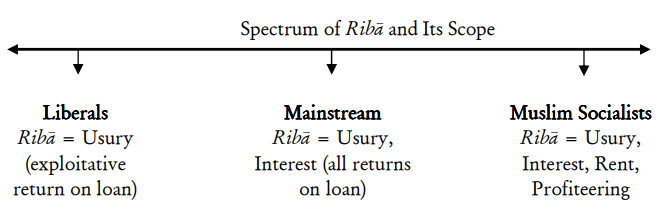
\includegraphics[width=\textwidth]{CourantsIslamContemporain/ImagesCourantsIslamContemporain/Riba.png}



The above differences have left scholars divided on several important questions that demand straightforward answers. Those questions include the following ones:
\begin{itemize}
    \item 
1. Is bank interest prohibited in the light of the Qur'an and the sunnah? If yes, how?
    \item 
2. Whether the Qur'anic term riba includes all kinds of interest rates or it relates only to the excessive interest rates?
    \item 
3. Whether the scope of riba extends to the interest charged and paid on business transactions in the banking system or is restricted to the interest charged on consumption loans only?
    \item 
4. Does Islam allow loan transactions? If yes, how and in what form?
    \item 
5. Is paying interest a lesser evil as compared to charging it?
    \item 
6. Is borrower always \textit{mazlum} (a losing party) in an interest bearing loan transaction?
    \item 
7. Does Islam allow indexation of loans on the grounds of inflation?
    \item 
8. Is credit-sale with higher deferred price as compared to the spot price allowed?
    \item 
9. Does Islam approve of “time value of money,” especially when charging higher deferred price is allowed in a credit sale?
    \item 
10. Are future currency contracts permissible in Islam?
    \item 
11. How and to what extent is salam transaction permissible?
\end{itemize}


These are but a few questions.
\begin{Synthesis}
We show in this paper that whatever confusion prevails among contemporary scholars on this subject is the outcome of following an inadequate methodology for determining the meaning and scope of riba.
\end{Synthesis}
 In fact, this methodology has mystified the nature of riba, which is otherwise clear when viewed from the methodological view point of the eminent Muslim jurists of the past. The mystification is such that not only it results in confusing answers to these questions but it also begets confusing questions. Unfortunately, the confusion has built up to the extent that the Federal Shariat Court of Pakistan has been struggling to come up with a definition of riba. It is in this background that this paper attempts to explain:

(1) the contemporary Islamic economists' methodology of interpreting and classifying riba; (2) why this methodology is wrong and insufficient; (3) the methodology of understanding riba on the pattern of Muslim jurists of the past; (4) that the methodology given by the Muslim jurists is coherent and compact.

The reader will encounter a number of arguments in this paper that are advanced by those who justify bank interest. Since the paper deals with the legal substance and not with the economic merits of arguments, hence we will restrict ourselves to the legal analysis of those arguments and leave aside their economic analysis and rationale, which require an altogether different methodology. Any legal system has three aspects: (1) what: the legal rulings (i.e., ahkam); (2) how: the rules of deriving those legal rulings (i.e., usul al-fiqh); and (3) why: the underlying rationale(s) and wisdom behind the legal rulings (i.e., hikmah)

It is important not to mix these aspects. The present study deals with the first two aspects of the issue of riba. Moreover, the classification of riba discussed in this paper is primarily based on the methodology of Hanafi jurists for ensuring analytical consistency. We presume that a school of law represents an internally coherent system of interpretation and that mixing up the views of the various schools results in inconsistencies.7 However, views of the other schools have been briefly mentioned in the footnotes wherever required. Finally, the paper does not attempt to show that the Hanafi jurists' approach is superior to all others, rather it explains that the classical jurists' approach (whether Hanafi, Maliki, Shafi‘i or Hanbali) to understanding riba is superior to that of the modern scholars. The methodology of these jurists share several common results that are important in order to answer the above questions.

Following section outlines the method adopted by modern Muslim scholars and economists. The next section discusses problems in this methodology and develops the skeleton for the methodology that is then applied in the coming section, which details out the general rules of riba alongside their resulting implications. The last section concludes the paper by giving a comprehensive definition of riba based on discussions in sections three and four.


\newpage
\subsection{Outline of the Mystifying Methodology}

Imran Ahsan Khan Nyazee\sn{\href{https://en.wikipedia.org/wiki/Imran_Ahsan_Khan_Nyazee}{Pakistan} Nyazee's academic career was inspired by the work of Abdur Rahim. Nyazee argues firstly, that due to its unique set of principles of interpretation, each school of Islamic law represents a theory of law unto itself. Secondly, he points out that Istiḥsān cannot be understood without understanding of the workings of qiyās. It is, therefore, difficult to accept that there was no system of interpretation before al-Shāfi‘ī's time. Thirdly, he concludes that the uṣūl al-fiqh never existed. Furthermore, Nyazee describes beyond the individual fikh of each school of law, another theory of interpretation called maqāṣid al-sharī‘ah (theory for the purpose of the sharī‘ah) which was developed by al-Ghazālī. Nyazee has written and self-published on a number of aspects of Islamic law. He agrees with most Muslim scholars that strictly speaking, selling money (taking interest) is prohibited, according to Islamic law. Some point out a difference between the treatment of riba in the Qur'an versus the Sunnah but Nyazee the two approaches are actually one and the same.Nyazee also proposes that all loans (except those of a charitable nature without a fixed period of repayment) and therefore all banking is prohibited and unIslamic. Nyazee is equally intolerant of murabaha, the Islamic system of business where in-put costs and mark-ups are made transparent between vendor and buyer. He argues riba will inevitably enter such transactions.[10] He extends the prohibition to the creation of wealth on the basis of debt and the fractional reserve banking system. These elements along with zakat (the system of alms-giving) he says, are the differences between Islam and capitalism. He advocates the use of the gold and silver dinars and dirhams as the currency of the Muslim community. Nyazee would also prohibit the corporation or 'legal personality' under Islamic law.} explains that the methodology adopted by modern scholars for determining the meaning of riba is the same, though they disagree in their conclusion regarding whether or not bank interest is riba.8 The fundamental problem of their methodology lies in overlooking the inherent link between the Qur'an and sunnah. This methodology of interpreting riba was initiated by Muhammad Rashid Rida (d. 1935) \sn{voir p. \pageref{Theol:Rida} Frère musulman pas le voyage en Europe. Plue el manar un commentaire coranique, sensé être l'héritage d'abdu}, which goes as follows:9

\paragraph{Lecture de Rida El Manar}
Riba is classified into two categories, riba of the Qur'an (also equated with riba 'l-nasi'ah, i.e., interest on loan transaction) and riba of hadith (equated with riba 'l-fadl, i.e., interest on exchange transaction).

Rida begins with literal meaning of the word riba (excess) and then traces some riba-based transactions practiced by Arabs during the time of Prophet (peace be on him). Rida, relying on some commentators of the Qur'an, asserts that the Qur'anic verse regarding riba deals with a specific practice of Arabs known as credit-sale where the payment of price is deferred to a future period while delivery of goods takes place on spot. Because a seller is allowed to charge whatever price he wants in a sale transaction, no riba is involved in the original price negotiated between the two parties-any excess in future price becomes part of the price. However, they used to increase the price excessively whenever the debtor would be unable to settle his debt obligations at the end of payment period. The debtor was given the option, “Will you pay the debt or increase the amount in lieu of delay?”

For Rida, it was this excessive rate (doubling and multiplying) of interest in debt-based transactions added to the original sum at the end of payment period which was prohibited by the Qur'an (he called it riba 'l-jahiliyyah).10 From this, he concluded that the bank interest is not the same riba that was deemed impermissible by the Qur'an because (a) it is neither doubling and redoubling of rates (b) nor the excess is stipulated in the initial period of the banking transaction-he assumes that the initially added interest is part of the principal or original sum just like the original sum in case of credit-sale. 
\begin{Synthesis}
Hence, for Rida, only compound interest is prohibited.
\end{Synthesis} 

Other scholars, supporting Rida's view, added that business loans were not common among Arabs as theirs was a subsistence economy; loans were largely taken by poor people for consumption purposes on interest and whenever they were unable to repay them at due time, excessive interests were added to the original sum. Hence, it was this type of interest that was declared prohibited by the Qur'an and it has nothing to do with the modern commercial loans, \textbf{which are mutually beneficial for both parties.}11

Having ascribed this meaning to the Qur'anic word riba on the basis of some historical traces, Rida then explains the form of riba declared impermissible in the sunnah as a distinct prohibition from that of the Qur'an.
\begin{Def}[Riba] Usure, profit ou gain réalisé sur un prêt.
\end{Def}

\begin{Def}
[Riba al-buyu] : Usure. Opération de vente dans laquelle une matière première est échangée contre la même matière première mais en quantité différente et la livraison d’une des matières premières est postposée. Pour éviter le riba al-buyu, les matières premières échangées par les deux parties devraient être en quantités égales et l’échange devrait être instantané. Riba al-buyua a été condamné par le Prophète Muhammad afin d’éviter que le riba (intérêt) n’affecte insidieusement l’économie.
\end{Def}
\begin{Def}[Riba al-duyun] : Usure d’une dette.
\end{Def}
 
\begin{Def}[Riba al-fadl] : La différence de quantité entre deux biens échangés et comportant du riba.
\end{Def}
\begin{Def}[Riba al-nasiah] : La différence de paiement liée au report de deux biens comportant du riba
\end{Def}\mn{cf Glossaire des termes financiers  Islamiques \href{https://www.cairn.info/la-banque-et-la-finance-islamiques--9782804167042.htm}{Banque et finance islamique} } He calls it \textit{riba 'l-fadl} which emerges in the exchange of two counter values of the same or different species and hence also called \textit{riba 'l-buyu‘}.12 The position of Rida, which may be termed as minority view, is summarised in figure 2.


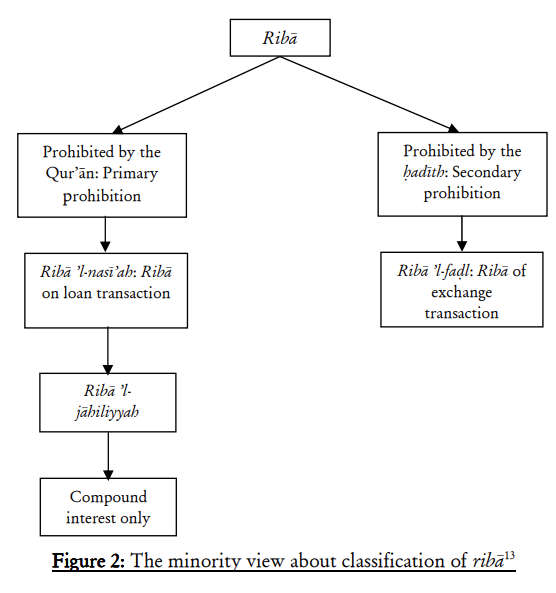
\includegraphics[width=\textwidth]{CourantsIslamContemporain/ImagesCourantsIslamContemporain/RibaRida.png}

Thus, Rida dichotomised the two concepts of riba, one attributed to the Qur'an and another to the sunnah. He finally declared the first one as real or explicit riba while latter as lighter or implicit riba.
\textbf{
Though the majority of contemporary scholars did not agree with the conclusion drawn by Rida about legitimacy of bank interest, however they adopted his methodology of classifying riba. The only difference in their opinion is that riba of the Qur'an includes all rates of return on loan and it is not merely restricted to the compound interest of jahiliyyah}\sn{la période pre islamique}


To them, business loans were a part of Arab's economy and any contractual return to lender is unfair because this is tantamount to refusing to share business risk with the borrower. We can depict their views in figure three.
\begin{Synthesis}
On a donc un nouveau problème, le pret commercial lié avec l'industrie et face à ce nouveau problème, une lecture de Rida qui est assez positive (Riba = Excess) mais qui note une différence entre Coran et Sunna) et fait une distinction entre les deux, reprises ensuite par les autres légistes, mais en repartant d'une lecture stricte du Riba comme intérêt. Il conveint d'articulier Coran et Sunna de façon non parallèle mais l'un par l'autre.
Il convient de montrer l'évolution du prêt commercial au XIX
\end{Synthesis}
Because the sunnah is not linked with the Qur'an in this methodology, both the minority and majority Muslim economists have struggled to explain as to why someone would engage in exchange transactions of the forms mentioned in hadith. Some opined that these transactions are declared impermissible because they may open the path for the “real riba” (i.e., riba of the Qur'an).


14 Others assumed that it was meant to discourage the practice of barter exchange and promote market exchange through a medium of exchange.15 Yet another view argues that it eliminates the possibility of benefiting from asymmetric information of the contracting parties.16 The truth is that none of these explanations makes the point.

2.1. The Nature of Debate within Minority and Majority Schools

The debate that has taken place within the followers of this mystifying methodology on the issue of why or why not bank interest is riba may briefly be summarised here. As explained above, Rida asserted that bank interest was not included in the Qur'anic concept of riba of debt because it was different from the riba that was charged by Arabs on credit-sale transaction by doubling and multiplying the price whenever the debtor was unable to settle his debt at due time and asked for relaxation in payment period.18 Rida explained that the Qur'anic verse “Allah has permitted bay‘ and prohibited riba”19 referred to this riba. To strengthen his case, he argued from the verse: “O Believers! Do not devour riba doubled and multiplied and fear God so that you may prosper.”20

This verse complements the former verse in the sense that what was implicit in the first verse was made explicit in the latter-both verses referred to the practice of doubling and multiplying of interest and none of them forbad the bank interest.

How do the majority of scholars respond to this argument? For example Usmani notes the Qur'anic verse:

O you believers! Fear God and give up riba that remains outstanding if you are true believers. Behold! If you do not obey this commandment, then God declares war against you from Himself and from His Prophet. But, if you repent (from riba), then you are entitled to only your principal amounts. Neither should you inflict harm to others, nor others should do harm to you.21

The argument is based on the emphasised words ‘you are entitled to only your principal amounts (ra's al-mal)'. He infers from these words that the rightful entitlement of lenders is the original sum advanced; he cannot charge any increase whether small or large (doubled and tripled). To him, the verse (3:130) forbids a severe form of riba where interest is multiplied, but it does not restrict riba to this specific form. Hence, bank interest falls within the purview of the Qur'anic verse “Allah has permitted bay‘ and prohibited riba.”22 They are also of the view that charging interest on commercial loans was also practiced by Arabs.23

Does the above analysis of mainstream scholars guarantee the prohibition of bank interest? We are afraid it does not. Their arguments rest on two assumptions:

(1) The verses (2:278-79) address the issue of loan-transaction.

(2) Ra's al-mal (principal amount) can only refer to the original principal advanced in loan.

Both of these assumptions are problematic. Following submissions can be made against them:

(a) If the meaning of the verse is to be determined with reference to historical practices, one can equally claim, just like Rida, that the verse is not about loan transaction but about credit sale. In that case, ra's al-mal is not referring to the principal amount lent; rather, it is the deferred future price of the goods sold. On which legal grounds or facts can this claim be dismissed?

(b) Further, this deferred price might include increase over and above spot price. Hence, the future price could consist of two components: spot price plus some additional profit. The sum of these two would constitute ra's al-mal (principal amount) in this transaction (i.e., principal amount in credit sale (ra's al-mal) = spot price + extra profit)

Whenever a debtor was unable to repay full amount, further multiplied increase was added to this original sum, Rida called it interest. This would increase the due amount to: total amount after increase added due to delay, which is interest in addition to ra's al-mal.

Using this structure, one can then argue that the initially added interest in a loan transaction is equivalent to initially added “extra profit,” which becomes part of ra's al-mal. Therefore, entitlement to the ra's al-mal means entitlement to the simple interest, as claimed by Rida.

(a) The only legal justification for ascertaining that the verse is about loan transaction is based on the words “ra's al-mal” (principal amount). But how can it be settled that ra's al-mal here means ra's al-mal of a loan transaction? This question is important because a number of transactions constitute a component of ra's al-mal. For example, there is ra's al-mal both in mudarabah and musharakah contracts. How to exclude these forms of ra's al-mal from the purview of the Qur'anic verse? If someone says, “This verse is about loan, so ra's al-mal refers to that of loan contract and not of mudarabah and musharakah,” he is clearly arguing in circularity. The argument goes like this:

Q: How do we know that the verse is about loan contract?

A: Because the verse talks about ra's al-mal.

Q: How do we know that ra's al-mal here refers to that of loan?

A: Because the verse is about loan contract!

A circular argument is no argument.

(b) Muslim Socialists could maintain that ra's al-mal means principal amount of all business contracts. Therefore, it is not legitimate to charge any excess over and above principal amount, no matter it is mudarabah, musharakah or ijarah.

Not only that the analysis of mainstream scholars does not necessarily imply the prohibition of bank interest, it leads to a set of unsettling arguments that have left Islamic economists bewildering about some basic issues. For example,

(1) Even if it is agreed that ra's al-mal means principal amount of a loan transaction, does it mean “nominal” amount or the “real” (inflation adjusted) amount? Again, what are the legal grounds to settle this issue? Because there are no clear-cut legal grounds available in this methodology, we see scholars are divided on this subject matter-some allow indexation of loan against inflations while others do not.

(2) What about the question of “time value of money?” This question poses challenge for Islamic economists because they, as a rule, approve the practice of charging higher price in credit-sale and murabahah.

(3) The Lawgiver has allowed salam, what are the legal grounds for not extending this permission to currency salam (future currency contracts)?

Undoubtedly, majority view has addressed these issues, but the answers do not seem to be stemming out of a coherent analytical legal system. This approach is often found mixing up legal analysis with economic analysis. This missing coherent analytical legal system is the root cause of most of the mystification that has prevailed all over. It is an unfortunate state of affairs and it is high time to demystify things.

3. Methodological Assumptions of Premodern Muslim Jurists (Fuqaha') for Understanding Riba

To understand the method used by the eminent premodern Muslim jurists for understanding riba, three methodological issues (MI) need to be clarified. They are explained by Nyazee in detail.24

1) Link between the Qur'an and Sunnah

The methodology adopted by the modern Muslim scholars and economists is misleading because it delinks the Qur'an and sunnah. It assumes that the meaning of riba is different in the Qur'an and sunnah, which is not the case. To explain the nature of error made by both the groups, it should be noted that Muslim jurists (fuqaha') classified riba in the category known as mujmal (unelaborated)25 whose meaning and scope cannot be determined without explanation (bayan) of the Lawgiver (Shari‘). The famous hadith (as given in footnote 1) that explains different usurious transactions actually does not add something to the Qur'anic word riba. Rather, it defines its meaning and scope.

Thus, while to the contemporary scholars the meaning of riba is known independent of hadith and they see hadith as adding some more cases to the Qur'anic concept of riba, the jurists say that hadith is the definition of the term riba used by the Qur'an. Thus, riba 'l-nasi'ah and riba 'l-fadl both are included in the Qur'anic concept of riba.

2) Relationship between Loan and Bay‘ (Exchange)

Loan is also classified as a form of exchange transaction (bay‘)26 by Muslim jurists. The scope of this paper does not allow detailed analysis of this assertion.27 For descriptive purposes, it can be seen that a loan of Rs X is an exchange of Rs X today with Rs X after time deferment (and with Rs X + Y if interest payment of Rs Y is included). Figure 4 depicts this nature of loan transaction by illustrating a loan transaction between Mr. A and B:

3) Skeleton of a Coherent Legal System

A coherent shari‘ah-based legal system consists of a set of general rules, called

‘azimah by the jurists, supplemented by some exemptions to these laws, called rukhsah. In the words of Nyazee, ‘Azimah (lit. determination, resolution) is applied to mean a rule that is applied initially and for itself. Such rules form the backbone of the law. As against this, there may be a rule that goes contrary to the requirements of the initial rule, but is permitted by the law. This rule is considered to be a rukhsah (exemption) from the initial rule.28

This classification of ‘azimah (the higher or first order rules) and rukhsah (the lower or second order rules) is important for several reasons.

First, it explains the order in which the rules have to be applied.

Second, it explains why sometimes two opposing cases may be allowed within a given skeleton of law.

Third, the order of rules implies that an exception cannot be extended using any method of argument, whether analytical or analogical. On the other hand, extension of first order rules is legitimate by these methods. In other words, it is not allowed to build a sub-legal system based on exemptions because otherwise it starts negating the primary provisions and objectives of the law-an exemption from the general rule must remain an exemption.

Fourth, because of the logical hierarchy in the operations of ‘azimah and rukhsah, it is clear that an exemption from a rule cannot be used to nullify or change the shari‘ah status (hukm) of any other case that is derived from the general rules. Alternatively put, an exemption (a lower order rule) cannot prevail over the higher order rules.

Fifth, because all rules and exemptions are derived from nusus (the Qur'an and sunnah), hence the only justifiable exemptions are the ones, which are given in nusus (i.e., stated by the Lawgiver Himself).

We call these nusus the “facts” of the shari‘ah-based legal system in this paper. Given these “legal facts,” the task of a jurist is to derive those general rules (‘azimah) from the facts, which render these facts internally consistent and extendible on the one hand and highlight the exemptions (rukhsah), if any, on the other.29 Finally, the general rules and exemptions generate some implications, called ahkam. This skeleton of a shari‘ah-based legal system is illustrated in Figure 5. We apply this skeleton in this paper to elaborate riba.

The relevant “legal facts” used by premodern Muslim jurists to derive general rules and exemptions are quoted at the relevant places in this article. We are now in a position to take on the issue of derivation of the general rules and the implications from those “facts.”

4. Underlying Rules behind the System of Bay‘ in Jurists' Methodology

Our intention in this paper is to reveal that the apparently large and complicated system of legal injunctions (ahkam) is reducible to a few set of rules derived from fewer legal facts. We propose that a majority of ahkam (legal injunctions or provisions) governing economic transactions (buyu‘) can be derived from three broad rules:

1. Rules of riba mentioned in the sunnah. This is not a single rule, rather a set of rules as explained below.

2. Rule about the sale of goods not possessed by a person.

3. Rule about exemption that an exemption is to be treated as exemption.

Before explaining these rules, we first explain the context of the Qur'anic verses that underlies the jurists' methodology of riba to clarify the misconception that the relevant verses of Surat al-Baqarah are about loan transaction and not exchange (bay‘).

4.1. The Context of the Verses of Surat al-Baqarah

The Qur'an states that the disbelievers said, “Verily, bay‘ (sale) is just like riba.” In response to this, it was said, “Allah has permitted bay‘ and prohibited riba.” To understand why the disbelievers said this, consider these three transactions:

(a) A gives B 100 grams of gold in exchange of 110 grams of gold to be paid after one year. This is primarily a sale contract as explained previously (i.e., exchange of 100 grams gold with 110 grams gold with time lag) and involves riba (how, this will be explained in the next section but take it for granted for the moment).

(b) A asks B for 100 grams of gold in exchange of, say, 500 kg wheat at spot. This is a legitimate regular sale contract.

(c) A demands from B 110 grams of gold in exchange of 500 kg wheat for payment of price after one year: this is credit sale contract with higher deferred price as compared to spot price and is also legitimate (this is explained in section 4.3).

The credit sale was a common practice among Arabs and, therefore, they were confused as to why the transaction (a) is impermissible and (c) is permissible while the two are quite similar in nature (i.e., both are credit sales and both involve access payment). In (a), 10 grams of additional gold are paid as counter-value for 100 grams of gold for a delay of one year and similarly 10 grams of gold are paid for a delay of one year in transaction (c). It is for this reason that disbelievers said, “Verily sale is just like riba!” That is, transaction (c) (i.e., the credit sale) is similar to the transaction (a). The technical reason for allowing transaction (c) and forbidding (a) is the similarity of genus which is explained by the sunnah. This is explained in the next sections in detail, but the important point to note here is that the assumption that the Qur'anic term riba is not about sale contract, rather it is about debt, is not implied by these verses.

Thus, the verse says that Allah has approved all forms of buyu‘ (exchange transactions) except those which involve riba.30 The natural question then arises: what is this thing called riba? Has the Qur'an given any definitive description of riba?

One may make one of the two assumptions here. First, the concept of riba was largely a sort of common knowledge for everyone and, hence, it required no legal description by the Qur'an. That common knowledge is traceable by an examination of historical record of Arabs which provides sufficient legal foundations for determining the meaning of riba. As far as the details of riba in the sunnah are concerned, they were additions over and above to that common knowledge of riba and most of these additions were unknown to the Arabs. The liberals and mainstream scholars share this assumption and we believe that this assumption constitutes what we called the “mystifying methodology.”

Second, some forms of riba may be or actually known to the Arabs but these do not set the legal standard against which the Qur'anic concept of riba is to be determined. As it is a legal term, its meaning has to be sought from the Lawgiver. In technical sense, the jurists call it mujmal (unelaborated) for which elaboration (bayan) is sought from the Lawgiver. This elaboration of the legal meaning of the Qur'anic term riba is given by the sunnah. After this elaboration by the Lawgiver, its meaning is determined definitively and it becomes mufassar (elaborated). This is the methodological assumption that the jurists use not only for defining riba but also for other legal terms of the Qur'an, such as salah, zakah, and so on.31 Thus, according to this second assumption, the practices and concepts of Arabs may be referred by the Qur'anic concept riba but it is not the benchmark against which we assign legal meaning to the Qur'anic terms.

For example, the Arabs had some concepts about how to offer salah (prayer), but this information does not define the legal meaning of the Qur'anic term salah nor is this concept limited to this information set. Similar is the case with riba. The Arabs might have been aware of some forms and practices of riba but that does not constitute the legal definition of riba. When the jurists classify a term as mujmal, they mean that this term is a technical legal term and its meaning should be determined with reference to the words of Lawgiver Himself, neither by the linguistics (dictionary) nor by the historically known social concepts and practices that hover around that technical term. It should be emphasised here that considering riba as mujmal does not mean that the Arabs did not know the meaning of this word at all. Nor does it mean that the pre-Islam Arabs did not identify certain transactions as riba-in fact they did and the jurists did consider it part of riba.32

It only means that the meaning of riba in Islamic law is not limited to, and is not based on its usage in the pre-Islam Arabia. The Qur'an and the sunnah added several shades of meaning to this concept. That is why, it became a “technical term” of Islamic law. Hence, its meaning and scope cannot be determined by its dictionary meaning or its practice and understanding by the pre-Islam Arabs. Rather, it must be determined by the Qur'an and the sunnah, like any other legal term such as salah and zakah. Just as we cannot classify concept salah as salah of the Qur'an and salah of hadith, similarly we cannot dichotomise riba. Once it is established that the meaning of riba must not be gathered from pre-Islamic usage and practices but from the Qur'an and the sunnah, the next question is: how to explain the various usages of riba in the Qur'an and the sunnah? The answer, as per the well-established methodology of the jurists, is to consider the sunnah as the elaboration of the mujmal verses of the Qur'an.

This methodology is employed by the jurists for determining the meaning and scope of salah and zakah as well as riba. Let's follow through the path of righteous ones here and have its blessings.

4.2. General Rules of Riba When Transacted Species are Same

Keeping these in mind, one has to understand the classification of riba in the system of Muslim jurists. Because the sunnah defines riba, note the words of hadith,

When you exchange gold for gold, silver for silver, wheat for wheat, rice for rice, dates for dates, and barely for barely, then exchange like for like (in equal measure) and exchange them hand to hand (at spot), else it will be riba.33

To understand what it says, consider these transactions:

1) exchange of 1 gram gold for 1 gram gold on spot;

2) exchange of 1 gram gold for 2 grams gold on spot;

3) exchange of 1 gram gold at spot for 1 gram gold with delay;

4) exchange of 1 gram gold at spot for 2 grams gold with delay.34

As per the hadith, the first transaction is allowed; the second one is disallowed because it involves excess in measurement/quantity (called riba 'l-fadl); the third transaction is also impermissible because the hadith says that the exchange of homogeneous goods is allowed in equal measurement provided it is on spot; therefore, this transaction involves the riba 'l-nasi'ah (i.e., riba of delaying); finally, the fourth transaction involves both types of riba. These transactions provide two guiding rules (R):

R 1.1) Goods of the same species cannot be exchanged immediately unless their measurement (in terms of weight or volume) is same.

R 1.2) Goods of the same species cannot be exchanged with time lag, even with same measurement.

4.2.1. Implications

Five important implications (I) should be noted.

I. 1) Impermissibility of Market for Loanable Funds

Application of rule 1.2 gives the important implication that loan, with or without interest, is prohibited in Islam because, as explained above, a loan is an exchange of homogeneous goods with time lag. Does it mean that loaning is not allowed in Islam under any circumstances? Of course, this implication of the general rule is at odd with a number of legal facts (nusus), which promise reward for offering loan to the needy ones. How to reconcile these apparently contradictory legal facts now? This is where the concept of rukhsah (exemption) is activated by the jurists. Though loaning is against the general rule (‘azimah) given by the Lawgiver, yet it is allowed by Him as an exemption from this prohibition if it takes the form of benevolent giving (tabarru‘ or sadaqah).35 Loan is classified as tabarru‘ if:

(a) it is out of the intention of benevolence to the other person (i.e., the lender consciously bestows upon the borrower the benefits associated with his asset);36

(b) no increase in its value is stipulated, else it would cease to be benevolent and would involve riba 'l-fadl; and

(c) no contractual time limit is stipulated, the lender can ask for his asset anytime he wants.37 Stipulating (legal) time constraint in loaning activity makes it a business transaction as per the application of general rules of shari‘ah and, hence, unlawful because in that case it is simply the exchange of homogeneous goods with time delay, which is not allowed, whether or not interest factor is included. Moreover, making the time period binding would imply that the lender is forced to do, or to continue with, an act of charity. This is against the very nature of charity.

In short, this principle implies that Islamic law does not permit the “market for loanable funds.” It sees loaning as an act of benevolence, especially in favour of one's relatives.38 Stated alternatively, loan is purely a social transaction (a means of tying and strengthening social bonds) in Islam and not a business. It was in this social transaction capacity that the institution of loan prevailed for thousands of centuries not only in Muslim societies but also in other civilisations of the world until the emergence of capitalism in the fifteenth century.39 Note that this important result (impermissibility of the market for loanable funds) does not follow directly from the classification of modern scholars of Islamic economics, as the majority view allows interest-free non-benevolent loans as a general rule and not as an exemption.

This implication answers one of the important arguments in favour of bank interest given by some economists. The argument says that interest should be allowed in shari‘ah because interest is the price of capital and without interest the market for loanable funds cannot be equilibrated. Because we are not dealing with the economic merit of arguments in this paper, we ignore its economic substance and comment on its legal merit only. It is clear from the above implication now that this argument has no shari‘ah basis because shari‘ah does not allow market for loanable funds to begin with, let alone equilibrating it from shari‘ah perspective.

Before moving on to the next implication, the important implication and exemption regarding loan transactions be noted:

I 1.1) A loan transaction is prohibited, whether or not interest factor is added to it.

I 1.2) A benevolent interest-free loan is recommended as an exemption to the general rules of riba by the Lawgiver.

I. 2) Impermissibility of Bank Interest

All forms of bank interest, whether simple or compound, are prohibited by Islam as per Rules 1.1 and 1.2. Similarly, the fact whether loan is made for business or consumption purposes makes no difference to this result. There remains no confusion about these conclusions if the shari‘ah rules are applied with consistency. In fact, the practice of charging interest by the bank includes both kinds of riba and it, therefore, may be stated that it is the most comprehensive form of riba! This can be verified from the figure 6, which depicts detailed structure of riba-based transactions in case of homogenous goods (leaves aside heterogeneous goods for the moment).

I. 3) False Dichotomy between “Giving and Taking” Riba

The recipient of riba is not always the lending party as is usually perceived. It can be seen from above examples that in case of transaction (2) the lender is the beneficiary of riba, but in transaction (3) riba is received by the borrower, and finally both are its recipients in transaction (4). Hence, opinions such as “taking riba is a greater evil than giving it and, hence, paying interest to the bank is a lesser evil” are based on the fallacious assumption that it is only the bank that receives interest in a typical interest-bearing loan transaction. This wrong assumption is the outcome of using the wrong methodology outlined in section two.40

I. 4) Mutually Beneficial Riba is Prohibited

The view that bank interest realised in transaction (4) is or should be permitted (as claimed by liberal Muslim scholars) is implicitly based on the assumption that “two wrongs make one right”-that is, it assumes that mutually enjoyed riba of the lender and borrower can make this transaction acceptable while the matter of fact is that each of them is separately prohibited to begin with.

I. 5) Irrelevance of Time Value of Money

Following the wrong methodology has resulted in another confusing argument that the bank interest should be allowed because of “time value of money.” This argument is based on the presumption that Rs. 1 today is worthier than Rs. 1 tomorrow. Why? Economists believe that this is due to the subjective time preferences of an individual. A rational (i.e., self-interested utility maximising) economic agent is said to have positive time preferences in the sense that consumption today is preferred to consumption tomorrow because the latter is uncertain, which makes him impatient, thus he wants to have it today than tomorrow.

Another reason for having this positive time preference emerges from the institutional arrangements: if I have the option of earning some interest (say Rs. Y) on Rs. 1 by putting it in a bank account today, why should I lend it to someone for free? Putting Rs. 1 in a bank account will make it “Rs. 1 + Rs. Y” for sure (assuming away bank insolvency), say, after one year while lending it to someone will leave it worth Rs. 1. Hence, Rs. Y (which may be expressed in percentage) is the price that should be paid to the lender for a loan of one year, else it would be unfair with him. This argument is more of economic than legal in its substance, however, some comments can be made here to evaluate its legal substance in the light of preceding discussion.

The relevant part of the proposed argument is the second one (the institutional arrangement) because the first one is merely a subjective feeling, which may differ from person to person (as a matter of fact, not everyone prefers to consume more today than tomorrow). The argument presumes that there exists and should exist a well-established legally functional market for loan, which coordinates interest-based loan transactions. But just recall “I.1” that Islam does not approve of the market for loan to begin with. Eliminate this institution of market for loan, and the argument disappears. The point is that the concept of “time value of money” conceived in this economic sense is alien to the discussion of riba. Its validity presumes that there exists a legal institutional market for loanable funds where money is growing continually and, therefore, an individual always has the option of putting his money in that market.

Not only that this assumption is invalid from the point of general rules of shari‘ah as explained, it is also in contradiction with the ontological structure of the universe and economic facts.

The above is not the only format of this argument, it is phrased in some other shades as well. For example, it is stated that money could buy benefits and had the lender not lent it he could have benefitted himself. This implies that lending is an act of sacrificing the benefits associated with money. Therefore, the lender should be compensated for this sacrifice and interest payment is exactly that reward. This reward makes sense given that the borrower takes benefit out of money. The argument is valid to the point that money is beneficial to the lender and that if he makes the choice of not lending it, he can benefit from it. Moreover, it is also true that the borrower enjoys the benefits associated with the money. None of these facts is denied by the shari‘ah rules. But these facts alone cannot formulate the required case for this argument; it requires a moral statement in its premise to derive the desired conclusion.

To see this, note that the argument does not end here, after quoting these facts it then makes a moral assertion: “it is morally (and hence legally) right if money is lent for reciprocal benefits.” Addition of this moral statement is necessary for validating the conclusion that “interest is the just reward for lending.” But this moral assumption contradicts the general rules of the shari‘ah, which are laid down above. Seeking reciprocity in loan is exactly what that changes its status from tabarru‘ to loan as a business transaction and, hence, it becomes nothing but riba. The argument here is quite straightforward:

The owner of money is granted the right of benefitting from his money by shari‘ah rules; he is given the option of making a conscious choice of transferring the benefits associated with his money to another person as an exception to the general rules by the shari‘ah, but there is neither any general rule nor any exemption from the Lawgiver that assigns him the right of lending money in the name of the so-called “mutual benefits” (refer to I. 4 above). Legally speaking, this involves both riba 'l-fadl (because the homogeneous goods are exchanged at different rates) and riba 'l-nasi'ah (because time stipulation is invoked-the lender asks for the excess of measurement for parting with the benefits of his money for a specified time).

Another variant of this argument comes with the heading of “effects of inflation on money.” We deal with it in the next section.

4.3. General Rules of Riba when Transacted Species are Different

What about the exchange of heterogeneous goods? The last words of the hadith are as follows: “If these species differ, then exchange as you like as long as it is from hands to hand.”

They give an immediate rule:

R 1.3) Goods of the different species can be exchanged with difference in measurement.

This rule says that such goods can be exchanged at different rates as far as measurement is concerned. In other words, riba 'l-fadl does not apply in case of heterogeneous goods. Is riba 'l-nasi'ah (prohibition of time delay in payment) also not applicable in this case? Apparently, it seems that it is not because of the words of hadith, “exchange should be on spot.” This has an odd implication that credit sale (sale of goods against money where payment is deferred to future time period) is not permissible under the shari‘ah rules. This is so because credit-sale is an exchange of heterogeneous goods with time lag. But the legal facts reveal that the Lawgiver has allowed credit-sale.41 How to explain this? Is credit sale also an exemption to the general rule, like a loan transaction? The answer is: “No, it falls within the general rules.”

To see how credit-sale is permissible within general rules, one needs to dig deep into the issue of the underlying cause (‘illah) that the Muslim jurists derived from the sunnah to understand the system of riba. The relevant question facing jurists was: Is prohibition of riba restricted only to the six goods named in the hadith or is it extendible to other goods? The answer of the jurists is, yes, it is extendible and for this extension they derived the underlying cause due to which riba was declared prohibited by the Lawgiver. Keeping aside the technical details and arguments, it should be noted that some of the goods are measured in terms of weight while others are measured in terms of volume. In the hadith under discussion, gold and silver were weighable while the other four items were volumeable at the time of Prophet (peace be on him).42 Based on this classification, the jurists derived two further rules:

R 1.4) when species are different but their method of estimation is the same (such as gold vs silver or wheat vs rice), unequal quantities can be exchanged, provided that the exchange is immediate;

R 1.5) when species are different and their method of estimation is also different (such as gold vs wheat), unequal quantities can be exchanged with time delay.43

Thus, the credit sale is allowed due to the application of Rule 1.5. To see this, consider these combinations of transactions:

1) Exchange of 1 gram gold at spot for 2 gram silver on spot (method of estimation same)

2) Exchange of 1 gram gold at spot for 2 gram silver in future (method of estimation same)

3) Exchange of 2 kg wheat at spot for 1 gram gold/silver on spot (method of estimation different)

4) Exchange of 2 kg wheat at spot for 1 gram gold/silver in future (method of estimation different)

The first transaction is allowed but the second is not because when species are measured by same method (i.e., “weight” in this case), then difference in the measurement (fadl) is allowed but deferment (nasi'ah) is not permissible. The third and the fourth transactions are allowed because here not only the transacted species are different but also their method of measurement (one was measured in “weight” while the other in “volume”).

In short, when both of the similarity factors (i.e., species and method of measurement) are found, then both fadl (excess of measurement) as well as nasi'ah (excess of time delay or time deferment) are prohibited. When similarity of measurement is found alone, then fadl is allowed but nasi'ah is prohibited. Finally, when none is found, both fadl and nasi'ah are allowed. Figure 7 depicts all of these rules completely (discussion about the last layer of boxes on the right-hand side of this figure is coming next).

The preceding discussion shows that the hadith explaining the nature of riba was not about the actual practices of Arabs that begged some economic explanations with which Muslim scholars have been struggling. Rather, it stipulated the rules of exchange. It says, “If at all you make exchange transactions, here are the governing rules.” Thus, all transactions that correspond to these general rules are allowed while those in contradiction with them are prohibited (however, some are exempted by the Lawgiver).

4.3.1. Implications

Following implications are derived from the above rules. It is important to note that the first two transactions mentioned in sub-section 4.2 belong to the case when method of estimation of the heterogeneous goods is same while the latter two cover the cases when their method of estimation is different.

I. 6) Placement of Regular and Credit-Sale

Transaction (3) is categorised as regular sale transaction (usually termed bay‘) by the jurists. On the other hand, transaction (4) covers credit sale, which may take two forms: with or without extra profit margin as compared to the spot sale. Because both measurement as well as payment time differential are allowed in this case, hence credit sale of both forms is allowed.

I. 7) Placement of Currency Exchange

The remaining two boxes are relating to the exchange of currencies (termed as bay‘ al-sarf by the jurists). A detailed description of these requires an appreciation of some more technical classifications44 made by the Muslim jurists. However, they are beyond the scope of this paper. Suffice to say that the jurists divided all tradeable species into two: (a) currency items, which are used as means of exchange; they included gold and silver (though other goods may also be treated as currency in this system) and (b) non-currency items, (goods that are exchanged, and are not medium of exchange). They roughly included all but gold and silver.45 Given this division, the jurists broadly mention four types of transactions (buyu‘):

(1) Non-currency item in exchange of non-currency item-called barter exchange.

(2) Spot or delayed currency (say gold) in exchange of spot non-currency (say wheat) item.

(a) If both of them (gold and wheat) are exchanged on spot, it is called regular sale of goods, and

(b) if the currency price (gold) is delayed, this is called credit sale.

(3) Delayed non-currency item (say rice) in exchange of spot currency item (say gold). Here, the price of the good is paid on spot while its delivery is delayed. This is called bay‘ al-salam (advance payment) by the jurists.

(4) One currency (gold) in exchange of another currency (silver)-known as bay‘ al-sarf.

Rules regarding the first two have been discussed above. Here, we have to make some submissions regarding this fourth type of transaction. Because this transaction comes under the umbrella of “different species with same method of measurement,” it is clear from figure 7 that the excess of measurement is allowed in this transaction while time deferment is not. This gives two further rules under rule (1.4):

1.4a) If different currency items (such as gold and silver) are exchanged, then it is allowed to exchange them at any rate;

1.4b) if different currency items (such as gold and silver) are exchanged, then it is not allowed to exchange them with time deferment.

If it is accepted that modern currencies are just substitutes of gold and silver, then two further important results emerge from this discussion:

I 7.1) Future Currency Contracts are Prohibited

Rules (1.4a) and (1.4b) imply that the spot currency transactions are allowed while their future contracts (known as currency salam in Islamic finance literature) are prohibited in Islam as they come under the purview of riba 'l-nasi'ah.

I 7.2) Indexing of Loans is Prohibited

Indexing the value of the currency loans against some underlying assets (say gold) on the ground of inflationary pressures is not allowed. It is often argued that since the value of currency decreases over time due to the presence of inflation, hence an extra-payment equal to the rate of inflation, over and above the original sum given in loan, should be allowed in favour of the lender to keep his purchasing power. Again, because the economic merit of this argument is beyond the scope of discussion in this paper, we restrict only to its legal merit. If it is accepted that one rupee is legally nothing but equivalent of 1 unit of gold or silver (whatever that unit be), then Rules 1.1 and 1.2 (governing the loaning contract in gold or silver currencies) should automatically become operational.

Those rules imply that (a) loaning in the form of currency item is allowed if and only if equal measurement (whatever the unit of measurement) is returned; else it would be riba 'l-fadl; and (b) it is a loan made out of benevolence and not business intention (having time stipulation); else it would be riba 'l-nasi'ah. Hence, adding an extra amount to loan transaction in the name of “indexation” is but both, riba 'l-fadl (because of the excess of measurement) and riba 'l-nasi'ah (because the increase is time bound). 46 Again, let simplicity and sanity prevail.

I. 8) Placement of Salam

To see how the jurists accommodated salam in this scheme, note that there is nothing in the set of rules 1 (from 1.1. to 1.5) which forbids it. However, according to rule 2 (given at the start of this section), selling what one does not possess is not permissible and this is exactly what a salam transaction involves. Thus, a salam transaction should not be allowed as per the general rules of shari‘ah. We are once again faced with the same issue: salam is permitted in the “legal facts;” how and where to place it in the legal skeleton of the shari‘ah? Is there another general rule, which governs its permission as we saw in case of credit sale or is it an exemption from the general rule just like loan? The jurists' answer is the following: Salam is permitted as rukhsah-exemption from the general rules-by the Lawgiver.47

Because it is an exception, as per rule 3, it would be allowed only as “one of its kind” (sui generis) and cannot be used as justificatory mode for deriving more comparable transaction forms (e.g., currency salam). An exception to the general rule remains exception and does not turn into a rule for other cases because then it ceases to be an exception and creates a situation of self-contradictory general rules, which is not acceptable in any legal system. Thus, salam transaction is allowed as an exception for those transactions where (a) a currency item is exchanged against a non-currency item and (b) non-currency item is deferred while the currency-item has been paid at spot.48 This is what the exception is all about; one cannot extend this exception to the transaction types where currency items are exchanged with each other because that would violate condition (a) of the exception case.49

Figure 8 shows a map of interplay among legal facts (nusus), general rules, exemptions, and the derived implications related to riba and bay‘ that are discussed in this paper. This diagram shows that a rather complex looking system of ahkam (implications) showing up at the ending layer boxes of figure 8 emerge out of a set of general rules, which are derived to make underlying legal facts compatible with each other.

5. Conclusion: The Definition of Riba

We conclude this paper by elaborating a comprehensive definition of riba that can be inferred from the discussions in this paper. Let's quote it from al-Sarakhsi:50
\begin{Synthesis}
Riba in its literal meaning is excess... and in the technical sense (in the shari‘ah), riba is the stipulated excess without a counter-value in bay‘ (sale).51
\end{Synthesis}


Let's explain it noting several points about this definition:

(1) Muslim jurists do not introduce the word loan in the definition of riba because they categorise loan transaction under exchange (bay‘). Not appreciating this point resulted in the misconception that since the fiqh conception of riba does not deal with the subject of bank loans, it needs to be inferred directly from the Qur'an.

(2) Riba is excess, either in the form of quantity (qadr) or in the form of benefits of delay (nasa'). The first is called riba 'l-fadl while the latter is called riba 'l-nasi'ah.

(3) This excess is without any counter-value permitted by the shari‘ah. Thus, the excess of quantity paid in lieu of time delay in case of interest-bearing loan is not allowed because these two cannot be the legitimate counter-values (see I. 4).52 For a substance to be counted as counter-value, it must be recognised by the general rules of the shari‘ah to begin with.53

(4) The excess is stipulated in exchange. If the excess is granted voluntarily, it would not be riba.

We started off with specific questions in the introduction. The appendix lists down the answers to these questions in the light of the above definition of riba. It can be seen that once the discussion about riba is placed on the right track, right and clear cut answers start emerging automatically.

Appendix: Questions and their Answers that Follow from the above Analysis

Notes

1 For detailed arguments of this position, see Abu 'l-A‘la Maududi, Sud (Lahore: Islamic Publications, 2000), 110-12; M. Umer Chapra, “The Nature of Riba in Islam,” Hamdard Islamicus 7, no. 1 (1984): 3-24; Muhammad Shafi‘, Mas'alah-i Sud (Karachi: Idarat al-Ma‘arif, 1996), 43-47; Muhammad Ayub, “What is Riba? A Rejoinder” Journal of Islamic Banking and Finance 13, no. 1 (1996): 7-24; Muhammad Taqi Usmani, The Historic Judgment on Interest Delivered in the Supreme Court of Pakistan (Karachi: Idarat al-Ma‘arif, 1999), 12-16; Mohammad Nejatullah Siddiqi, Riba, Bank Interest and the Rationale of Its Prohibition (Jeddah: Islamic Research and Training Institute, 2004), 45-48; and Mahmoud A. El-Gamal, Islamic Finance: Law, Economics, and Practice (Cambridge: Cambridge University Press, 2006), 46-52. Within this category, there are further two approaches.

One approach that represents traditional ‘ulama' emphasises the resurgence of only those business contracts that were approved by the early Muslim jurists. It proposes profit-and-loss sharing (PLS) as an ideal alternative to riba. Though it does not deny the permissibility of other than PLS-based financing instruments such as murabahah and ijarah, yet it affirms that equity-based financing method is the primary means of achieving desirable economic objectives. The second approach is pragmatic one. It justifies a more liberal and flexible stance on structuring shari‘ah-compatible transaction forms that looks for financial engineering to meet all demands of modern banking customer.

2 Muhammad Rashid Rida (d. 1935) was among the foremost proponents of this theory. See his al-Riba wa 'l-Mu‘amalat fi 'l-Islam (Cairo: Dar al-Manar, 2007). Also see Sayyid Yaqub Shah, “Islam and Productive Credit,” The Islamic Review 47, no. 3 (1959): 34-37; Fazlur Rahman, “Riba and Interest,” Islamic Studies 3, no. 1 (1964): 1-43; Timur Kuran, “On the Notion of Economic Justice in Contemporary Islamic Thought,” International Journal of Middle East Studies 21, no. 2 (1989): 171-91; Izzud-Din Pal, “Pakistan and the Question of Riba,” Middle Eastern Studies 30, no. 1 (1994): 64-78; and ‘Abd al-Karim Athari, Sud Kiya Hay? (Mandi Baha' al-Din: Anjuman-i Isha‘at-i Islam, 2008), 8-12 3 Constant J. Mews and Ibrahim Abraham, “Usury and Just Compensation: Religious and Financial Ethics in Historical Perspective,” Journal of Business Ethics 72, no. 1 (2007): 1-15.

4 See Ghulam Ahmad Parvaiz, Nizam-i Rububiyyat (Lahore: Idara-i Tulu‘-i Islam, 1978).

5 Rafi‘ Allah Shihab, Kirayah-i Makanat ki Shar‘i Haithiyyat (Lahore: Kitab Ghar, 1981).

6 Ziaul Haque, “The Nature and Significance of the Midieval and Modern Interpretations of Riba,” The Pakistan Development Review 32, no. 4 (1993): 933-46.

7 For details, see Imran Ahsan Khan Nyazee, Theories of Islamic Law: The Methodology of Ijtihad (Islamabad: Islamic Research Institute, 1994), 9-12.

8 Nyazee, The Concept of Riba and Islamic Banking (Islamabad: Institute of Advanced Legal Studies, 1995), 11-19. Imran Ahsan Khan Nyazee (b. 1945) is a well-known scholar and a prolific writer on the subject of Islamic law and is a former Professor of law in International Islamic University, Islamabad. His major works include Theories of Islamic Law; Islamic Jurisprudence; Islamic Law of Business Organization; and The Concept of Riba and Islamic Banking. He also translated some of the classical texts on Islamic law and jurisprudence, including: Hidayah of Marghinani; Bidayat al-Mujtahid of Ibn Rushd; Amwal of Abu ‘Ubayd; and first two volumes of Muwafaqat of Shatibi.

9 Rida, al-Riba wa 'l-Mu‘amalat fi 'l-Islam, 69ff.

10 Period before the advent of the Prophet (peace be on him) is referred to as jahiliyyah (i.e., the period of uncivilised state of affairs).

11 Fazlur Rahman, “Riba and Interest,” 7-8.

12 In this regard, a hadith reads, “The Prophet said, ‘While exchanging gold for gold, silver for silver, wheat for wheat, barley for barley, dates for dates, and salt for salt, exchange like for like, in equal measure, and exchange from hand to hand. If these species differ, then sell as you like as long as it is from hand to hand.'” Muslim b. al-Hajjaj, Sahih, Kitab al-musaqah, Bab al-sarf wa bay‘ al-dhahab bi 'l-wariq naqdan.

13 Adopted from Nyazee, Concept of Riba.

14 Maududi, Sud, 118-19.

15 Chapra, “Nature of Riba in Islam,” 3.

16 Siddiqi, Riba, Bank Interest and the Rationale of Its Prohibition, 49-50.

17 Adopted from Nyazee, Concept of Riba.

18 Rida, al-Riba wa 'l-Mu‘amalat fi 'l-Islam, 69-70.

19 Qur'an 2:275.

20 Ibid., 3:130.

21 Ibid., 2:278-79.

22 Ibid., 2:275.

23 For details, see Shafi‘, Mas'alah-i Sud, 106-120 and Siddiqi, Riba, Bank Interest and the Rationale of Its Prohibition, 38-40.

24 Nyazee, Concept of Riba, 35-36.

25 Mujmal is a term used by Muslim jurists to refer to a Qur'anic term that begs its explanation through the words of Lawgiver (i.e., God and His Prophet [peace be on him]). One cannot interpret mujmal either by looking its meaning in the dictionary nor can its meaning be determined through historical practices at the time of revelation of the Qur'an. Mujmal can be elaborated only by the Lawgiver. Another example of mujmal is the Qur'anic term salah (prayer) which cannot be interpreted literally.

26 Bay‘ means exchange of counter values, and is not restricted to sale of goods/services. Abu Bakr b. Mas‘ud al-Kasani (d. 587/1191), the illustrious Hanafi jurist, defines bay‘ as “exchange of property with property” and then elaborates that the concept includes not only ordinary sale but also barter, exchange of currencies, advance payment and many other forms of exchange. Bada'i‘ al-Sana'i‘ fi Tartib al-Shara'i‘, ed. ‘Ali al-Mu‘awwad and ‘Adil ‘Abd al-Mawjud (Beirut: Dar al-Kutub al-‘Ilmiyyah, 1997), 6:532-33. Abu 'l-Hasan ‘Ali b. Abi Bakr al-Marghinani (d. 593/1197), author of the authoritative Hanafi manual al-Hidayah, also explicitly asserts that qard (loan) begins as an act of charity but becomes an exchange transaction in the end. al-Hidayah fi Sharh Bidayat al-Mubtadi (Beirut: Dar Ihya' al-Turath al-‘Arabi, n.d.), 3:60

27 See Nyazee, Concept of Riba, 45-46.

28 Ibid., 49.

29 The Hanafis use the methodology of istihsan (juristic preference) for ensuring harmony and analytical consistency within the law when general rules and legal facts seem to contradict. If something appears prohibited in the light of the general principles of law, but has been explicitly permitted by one of the texts (i.e., legal facts), the Hanafi jurists take the position that it is permissible as an exception to the general principle. They use the rule, “prohibited under qiyas but permissible under istihsan” for this purpose. Exceptions to the general principles are made on the basis of the text, consensus, necessity or some other “covered principle” (qiyas khafi), which needs to be uncovered. Muhammad b. Abi Sahl al-Sarakhsi is worth quoting here: “This [istihsan] is the evidence coming in conflict with that apparent principle (qiyas zahiri), which comes into view without one's having looked deep into the matter.

Upon a closer inspection of the rule and the resembling principles, it becomes clear that the evidence that is conflicting with this apparent principle is stronger and it is obligatory to follow it. The one who chooses the stronger of the two evidences cannot be said to be following his own personal caprices.” Muhammad b. Abi Sahl al-Sarakhsi, Tamhid al-Fusul fi 'l-Usul, ed. Abu 'l-Wafa' al-Afghani (Beirut: Dar al-Kutub al-‘Ilmiyyah, 1993), 2:200-202. Another important point made by al-Sarakhsi is that when the jurist uses istihsan and prefers the stronger rule, he abandons the weaker one and as such it is not permissible for him or his followers to follow the latter. He goes on explaining that when istihsan is carried out on the basis of a concealed or covered principle (qiyas khafi), the established rule does not amount to be an exception but becomes a general principle in itself.

Interestingly, not only the Hanafi jurists but also the Maliki jurists explicitly employ the principle of istihsan for resolving the apparent anomaly found in the legal facts where one set of nusus prohibits a loan transaction and another set of nusus allows it. They hold that it is prohibited as an exchange transaction but allowed as an act of charity.

30 Al-Sarakhsi interprets this verse as the following: “Trade is of two kinds: permitted (halal), which is called bay‘ in the law; and prohibited (haram), which is called riba. Both are types of trade. Allah informs us, through the denial of the disbelievers, about the rational difference between sale (bay‘) and riba, and says, ‘That is because they said, “Sale is like riba.”' He, then, distinguishes between prohibition and permission by saying, ‘And Allah has permitted sale and prohibited riba.' Through this, we came to know that each one of these is trade, but only one form is permitted.” Al-Sarakhsi, al-Mabsut, ed. Hasan Isma‘il al-Shafi‘i (Beirut: Dar al-Kutub al-‘Ilmiyyah, 1997), 12:1-2.

31 The famous Hanafi jurist Abu Bakr al-Jassas al-Razi (d. 370/980) says, “In the law (shari‘ah), it (riba) is applied to meanings in which it was not used in the language. This is indicated by the fact that the Prophet (peace be on him) termed nasa' as riba in the tradition of Usamah b. Zayd (God be pleased with him). He said, ‘Verily, riba is in nasi'ah.' ‘Umar b. al-Khattab, (God be pleased with him) said that riba had different forms and out of these salam in teeth, that is, in animals, is not concealed. ‘Umar also said that the verse of riba was one of the last to be revealed, and the Prophet (peace be on him) was taken away before he could elaborate the details for us. Therefore, give up riba and the suspicion of riba. It is established from this that riba became a technical term, for had it been governed by its original meaning in the language, it would not have been obscure for ‘Umar, who was fully aware of the names used in the language, being a native speaker.

This (the conversion of the word into a technical meaning) is also indicated by the fact that the Arabs were not aware of the sale of gold for gold and silver for silver with a delay (nasa') as riba, but this is riba in the technical meaning. If this (meaning of riba) is as we have explained it, then, it became like all the other unelaborated (mujmal) words that are in need of an elaboration (bayan). These are terms that have been transferred from the language to the law and assigned meanings to which the word was not originally applied in the language, like salah, sawm, and zakah. Such words are in need of a bayan and it is not proper to employ them in legal reasoning for the prohibition of any of the contracts, unless an evidence has been adduced to show that such a meaning is employed by the law.

The Prophet (peace be on him) elaborated on many occasions the intention of Allah in a verse, by way of an explicit statement or in response to a query (tawqif), and through these he has indicated the evidence (dalil). The (legal) meanings are, therefore, not lost to those who have knowledge when they employ legal reasoning.... In the technical sense, the word riba is assigned several meanings. The first is the one that was prevalent among the people of the jahiliyyah. The second is excess in the same species out of things measured and weighed, according to the view expressed by our (Hanafi) jurists.... The third is nasa' (delay), which is of several types.” Ahmad b. ‘Ali al-Razi al-Jassas, ed. Muhammad al-Sadiq al-Qamhawi, Ahkam al Qur'an (Beirut: Dar Ihya' al-Turath al-‘Arabi, 1992), 2:183-84. Al-Sarakhsi is also worth quoting here:

“Mujmal is the word the meaning of which is not understandable except by asking the one who used this word.... An example of mujmal is the saying of the Almighty: “He prohibited riba” as riba literally means excess but we know that this is not meant here because sale has been permitted for the purpose of excess. Rather, riba here means prohibition of a sale due to an excess without a counter-value stipulated in the contract; and this excess is either in the form of increase in measure or by way of delay.... It is obvious that this elaboration is not known by literal analysis. Rather, it needs a separate source. Hence, it is mujmal with respect to its intended meaning. The same is the case of salah and zakah. They are also mujmal because their original literal meaning is prayer and growth, but because of their use in specific legal acts, their intended meaning cannot be gathered from their literal analysis.” al-Sarakhsi, Tamhid al-Fusul fi 'l-Usul, 1:168-69.

32 See al-Jassas, Ahkam al-Qur'an, 2:183-84.

33 Muslim, Sahih, Kitab al-buyu‘, Bab bay‘ al-ta‘am bi Mithlih.

34 One can simply substitute “Rs.” for “gram gold” in these transactions if Rs. (currency) is treated as substitute of gold and silver currency.

35 The famous Hanafi manual Hidayah explains the position of a loan transaction in the following words: “It is an act of charity in the beginning and that is why it is not valid from a person who does not have the capacity to do charity, such as a minor or a guardian (of a minor). However, at the end, it becomes a contract of exchange because it turns into exchange of dirhams with dirhams with delay, and that is riba.” See al-Marghinani, 3:60. The commentators explain, “This necessitates invalidity of loan but the shari‘ah has recommended it and the whole ummah agrees on its validity; hence, we hold that it is valid but not binding (and can be terminated at will by any party).” Akmal al-Din Muhammad b. Mahmud al-Babarti, al-‘Inayah sharh ‘ala al-hidayah (Bulaq: al-Matba‘ah al-Kubra al-Amiriyyah, 1316 AH), 5:273. The same position is upheld by Maliki jurists.

Thus, the famous Andalusian Maliki jurist Abu Ishaq al-Shatibi (d. 790/1388) says, “There are many examples of istihsan in the law, such as loan, which is riba in reality because it is exchange of dirham with dirham with delay; but it has been permitted because it benefits and facilitates the needy.” Ibrahim b. Musa al-Shatibi, al-Muwafaqat fi Usul al-Shari‘ah, ed. Abu ‘Ubaydah Mashhur b. Hasan (al-Khobar: Dar Ibn ‘Affan, 1997), 5:194-95.

36 Jurists apply the rules of ‘ariyah (commodate-loan) on these transactions because it is the nearest match for qard and the only way to legally justify a qard transaction. Al-Kasani, 10:600.

37 In much the same way as time period cannot be stipulated in a contract of ‘ariyah because no one can be compelled to do or continue with an act of charity (tabarru‘). Al-Marghinani, al-Hidayah, 3:60. In other words, making the condition of time-period binding changes the nature of the transaction and it no longer remains tabarru‘.

38 This has some income distributional as well as social consequences.

39 For an analysis of the idea of “debt as a social construct” and the transformation of this social construct to the impersonal market form, see David Graeber, Debt: The First 5,000 Years (New York, NY: Melville House Publishing, 2011, 308-60.

40 This false dichotomy is also not consistent with a number of “legal facts” (nusus). For example, in a hadith the Prophet (peace be on him), after explaining the rule of exchange among six goods, said, “Whosoever paid more or demanded more, indulged in riba.” Muslim, Sahih, Kitab al-musaqa, Bab al-sarf wa bay‘ al-dhahab bi 'l-wariq naqdan. Both are treated equally because both are the participants of “market for loan” which is not allowed.

41 The validity of credit-sale is inferred from many facts. These include the general permissibility of sale transactions such as the words of the Exalted, “Allah has permitted sale” (2:275). The jurists hold that all sales are permitted except those which have been prohibited specifically, such as sales involving uncertainty (gharar) or which stand prohibited by the operation of other principles of law, such as the prohibition of riba. The analysis in text explains that credit sale does not fall under the prohibition of riba.

42 This is the Hanafi position. The other schools classify these six items in different ways, but interestingly all classify them into two categories. The below table summarises their positions:

School Position on Gold and Silver Position on other Four Items Hanafi weighable (mawzunat) volumeable (makilt) Hanbali weighable (mawzunat) volumeable (makilt) and countable (ma'dudt) Shfi'i currency (thaman) edibles (mat'umat) Maliki currency (thaman) storable edible items (mat'umat)

The net result is that all the four schools agree on the applicability of the rules of riba on gold and silver (though for different reasons) and they come up with the impermissibility of loan transaction. For the Hanafis, they are also applicable on all items that are either weighed or volumeable (whether they are food items or not, does not matter); the Hanbalis agree with the Hanafis but add a third category of the counted items; for the Shafi‘is, the rules of riba are applicable on food items (whether they are weighed, measured or counted does not matter); the Malikis agree with the Shafi‘is but add a proviso that these food items must be such that people generally prefer to store them. These differences have interesting implications for extending the rules of riba to cases other than the six items specifically mentioned in the traditions. For details, see Nyazee, Concept of Riba, 83-88.

43 Interestingly, although the four schools have determined different ‘illah (cause) for the operation of riba on gold and silver, yet a loan transaction even if interest-free remains prohibited for all the four schools. Thus, for the Hanafis and the Hanbalis gold and silver must be exchanged on spot because they are weighable items, the Malikis and the Shafi‘is deem it necessary because gold and silver are currency items. Resultantly, despite disagreement on the ‘illah of riba, all the four schools agree that a loan transaction is prohibited as an exchange transaction and permitted only as an act of charity.

44 These include the terms ‘ayn, dayn, and thaman. For an elaboration of the meaning of ‘ayn and dayn, see Nyazee, Concept of Riba, 54-57.

45 The jurists treat gold and silver as thaman (price/currency) in exchange with all other items. Even when they are exchanged with each other (as in the contract of sarf), both of them are treated as thaman. That is why they are called thaman mutlaq (absolute thaman). Fungible items (mithliyyat) are deemed thaman if they are exchanged with non-fungible items (qimiyyat). When a fungible item is exchanged with another fungible item, such as when wheat is exchanged with barley, the parties are at liberty to consider any one of them as thaman but they have to specify it in the contract. For details, see al-Kasani, Bada'i‘ al-Sana'i‘, 7:216-17.

46 The last two implications are based on the widely accepted assumption that modern currencies are just like gold and silver currencies and should be treated as their substitutes. See Ghulam Rasul Sa‘idi, Sharh Sahih Muslim (Lahore: Farid Book Stall, 1998), 4:350-361; and Muhammad Taqi Usmani, Islam aur Jadid Ma‘ishat-o Tijarat (Karachi: Ma‘arif-i Islami, 1999). Changing this assumption can change the implications. The alternative to this view is to accept that modern money is a promise of payment, which implies that it is an acknowledgement of debt. In that case, Islamic rules of hawalah (endorsement) transaction will be applicable. Accepting this position can allow the indexation of loans since money is now treaded as value of something which it promises and, therefore, a loan can be linked to the underlying promised asset.

However, accepting the premise that “modern money is debt” leads to the result that exchange of currencies is not allowed even on spot because of another general rule of the shari‘ah, namely, “prohibition of exchanging debt for debt” (bay‘ al-kali' bi 'l-kali'). The prohibition is reported in by many scholars of hadith. For instance, see ‘Ali b. ‘Umar al-Daraqutni, Sunan, Kitab al-buyu‘, Bab nahy ‘an bay‘ al-kali' bi 'l-kali'; Muhammad b. ‘Abd Allah al-Hakim, al-Mustadrak ‘ala 'l-Sahihayn, Kitab al-buyu‘, Bab nahy ‘an bay‘ al-kali' bi 'l-kali'. Thus, one cannot maintain both of these positions simultaneously; either he has to allow indexation of loans or he has to allow exchange of currencies. For details, see Nyazee, Concept of Riba, 96-114.

47 The jurists cite traditions of various Companions who report that the Prophet (peace be on him) prohibited them from selling what they did not possess but gave exemption for salam. Al-Kasani, Bada'i‘ al-Sana'i‘, 7:101-02.

48 Some other conditions are also applicable for the validity of this transaction but they do not relate to our subject matter here. For their details, see al-Kasani, Bada'i‘ al-Sana'i‘, 7:103ff.

49 A misconception prevails regarding the nature of riba due to a tradition, “there is no riba except in nasi'ah (deferred payment transactions).” These words of Ibn ‘Abbas constitute reason that can explain the adoption of wrong methodology by the contemporary Muslim scholars. It is inferred from this tradition that the primary form of riba deals with loan transaction, which is riba 'l-Qur'an. However, several points invalidate this inference as indicated by al-Sarakhsi. See al-Sarakhsi, al-Mabsut, 12:11-12. First, the words of the hadith are quoted from Ibn ‘Abbas who initially had this opinion but he reverted from this position later on when the hadith of riba was brought to his knowledge by Abu Sa‘id al-Khudri. Second, the ahadith of riba are quoted by several Companions of the Prophet (peace be on him) through several sources. Therefore, they cannot be ignored out rightly in favour of this isolated narration.

Third, hence, it is necessary to place these words of Ibn ‘Abbas appropriately within the legal structure of the shari‘ah. Thus, al-Sarakhsi points that the words relate to the exchange of heterogeneous goods measured similarly, because in that case there is no riba except in deferment.

50 Apçna²'

51 Al-Sarakhsi, al-Mabsut, 12:109.

52 That is why, the definition of riba in al-Durr al-Mukhtar, a later Hanafi text, is given as follows: “Riba is an excess without any counter-value recognised by shari‘ah, in favour of one of the parties in a transaction.” Muhammad Amin b. ‘Abidin, Radd al-Muhtar ‘ala 'l-Durr al-Mukhtar Sharh Tanwir al-Absar, ed. ‘Adil Ahmad ‘Abd al-Mawjud and ‘Ali Muhammad Mu‘awwad (Riyadh: Dar ‘Alam al-Kutub, 2003), 7:398-401.

53 For example, if a female sells her body in exchange of mangoes, this would not be legitimate. Nor will it be legitimate if A lends Rs 1,000 to B on the condition that B will repay Rs 1,000 plus a swine.

Appendix: Questions and their Answers that Follow from the above Analysis No Questions Answers 1 Is bank interest prohibited in the light Yes, it is prohibited, because it is of the Qur'n and the sunnah? violation of rules 1.1 and 1.2. 2 Whether the Qur'nic term rib It includes all forms of interests. includes all kinds of interest rates or it This is a necessary implication of relates only to the excessive interest rules 1.1 and 1.2. rates? 3 Whether the scope of rib extends to It extends to all kinds of loans, the interest charged and paid on commercial or consumption, as business transactions in the banking shown by the application of rules 1.1 system or it is restricted to the interest and 1.2. charged on consumption loans only? 4 Does Islam allow loan transactions? If Loan is against the general rules of yes, how and in what form? Islam. However, it is permitted by the Lawgiver as an exemption to the rule if it takes the form of tabarru'. 5 Is paying interest a lesser evil as No, it is not. The assumed compared to charging interest? dichotomy is wrong, as it has been clarified by I.3. 6 Is borrower always malm (a losing No, the borrower can also be the party) in an interest-bearing loan receiver of rib as per rules 1.1 and transaction? 1.2 (see I.3). 7 Does Islam allow indexation of loans No, it does not. The demand for on the grounds of inflation? loan indexation is invalidated by rules 1.4a and 1.4b. 8 Is credit sale with higher deferred price Yes, it is validated by the application as compared to the spot price allowed? of rules 1.4 and 1.5. 9 Does Islam approve of "time value of No, it does not. In fact, the concept money," especially when charging is alien to the subject matter of rib, higher deferred price is allowed in a provided both the concept of time credit sale? value of money and rules of rib are used appropriately. 10 Are future currency contracts No, they are not. It is violation of permissible in Islam? rule 1.4b. 11 How and to what extent is salam Rule 2 implies that salam is against transaction permissible? the general rules of the shar'ah but allowed as an exemption by the Lawgiver, hence, should remain exemption as per rule 3.
 \end{quote}
 
 
 \paragraph{Chapitre 8. Islam et assurances}
 LES CAPITAUX DE L’ISLAM  | Gilbert Beaugé
 \href{https://books.openedition.org/editionscnrs/871?lang=fr}{ Islam et assurances}
\begin{quote}
    
L’assurance est-elle légale du point de vue de la Shari’a ? Ce débat aujourd’hui encore est très vif dans les pays musulmans\sn{1 En fait, quatre éléments ont permis de classer les contrats d’assurance parmi les contrats interdits par le clergé islamique : a) l’imprécision (gharar), b) le jeu de hasard (gimar), c) l’usure (riba) et d) l’échange de choses équivalentes (bai al sain bil-dain). Le travail le plus complet à ce sujet est celui de Muhammad Baltagi, Uqud al-ta’ min wigha al-figh al islami Koweit, 1982. K. Krüger donne une bonne vue d’ensemble du droit privé des États régis par le droit égyptien. Certains problèmes comme celui du riba sont analysés de façon plus détaillée, cf. Recht van de islam, 1987.}. La fonction sociale de l’assurance est tout particulièrement perçue par la population musulmane, dans la mesure où les catégories classiques du droit musulman intègrent cette valeur. Cette fonction suppose l’utilisation du principe d’assurance et, même dans un pays aussi conservateur que l’Arabie Saoudite, on ne rencontre aucune réserve à l’encontre de l’assurance sociale\sn{2 Introduit par décret royal, pp. 98 sv., n° 746 du 5.09.1969.}. En revanche, on continue à y critiquer l’assurance privée et, de temps à autre, cette critique réapparaît dans d’autres pays islamiques.

 
2 L’assurance peut se définir comme les précautions terrestres que l’on prend à l’encontre des coups du destin et des pertes matérielles, autant d’épreuves envoyées par Allah comme le sait tout musulman pieux. De ce point de vue, l’assurance peut apparaître comme le renoncement à la croyance en une prédestination, l’abandon de l’espérance en une miséricorde ou, pour le moins, comme leur limitation. A ces problèmes de nature religieuse ou morale qui, dans des périodes difficiles, comportent également un élément politique, s’ajoute, pour le musulman, la difficulté à concevoir la notion de risque et à la démarquer de celles de jeu ou de pari, afin de pouvoir en saisir la signification fonctionnelle, en rupture avec les contrats spéculatifs qu’interdit la Shari’a\sn{3 Cf. à ce sujet Al Amin Al Darir, Al Gharar wa-athauhu fil-uqud fil figh al islami.}. La discussion sur ce thème, qui se fonde sur des textes classiques de la Shari’a remontant au Moyen Age, s’est développée à la suite de l’implantation des compagnies d’assurance européennes dans l’empire ottoman, au cours de la deuxième moitié du xixe siècle, et des tentatives d’innovation des réformateurs de l’Islam, au début de ce siècle. Une opposition de type nationaliste et pan-islamique se manifesta alors à l’encontre de ces institutions capitalistes et occidentales, qui jouera un rôle non négligeable.
 
\subparagraph{HISTORIQUE DE LA NOTION D’ASSURANCE DANS LES PAYS DU MONDE ARABE}

3 La première réflexion approfondie sur la légalité de l’assurance en pays islamique tint compte de façon singulière des exigences musulmanes. Dans son ouvrage Radd al Muhttar, Ibn Abidin, représentant de l’école officielle de droit Hanafi dans l’empire ottoman, suggère en effet le compromis suivant : il serait licite d’établir des contrats d’assurance portant sur les risques encourus à l’intérieur du royaume islamique – le Dar al Islam – à condition que ces contrats soient conclus avec une compagnie d’assurance ayant son siège hors des pays de l’Islam, dans le pays des infidèles. La prise en charge du risque devrait se faire au siège de la compagnie\sn{4 Cf. l’étude complète de C.A. Nallino, « Belle assicurazioni in diritto musulmano banafita », in Oriente moderne, vol. VII, Rome, 1947. pp. 446 sv.}.

4 On estimait ainsi satisfaire suffisamment les besoins pratiques en assurances nécessités par le trafic international des marchandises, à une époque où Constantinople, Beyrouth et Alexandrie, ports par où transitait le coton, étaient les centres essentiels du commerce britannique du Levant, alors que le commerce français était davantage orienté vers les côtes d’Afrique du Nord.
 
5 Ce n’est que relativement tard, vers 1890, bien après la fondation de banques ou la création de filiales bancaires (1850), que fut créée une compagnie d’assurance à Alexandrie5. L’initiative en fut prise par trois Libanais qui reprirent la filiale d’une petite société anglaise s’occupant d’une affaire d’assurance-vie en Égypte, pour l’étendre, à partir de Beyrouth, à l’ensemble de la Syrie. Au début du siècle, au moment même où des sociétés françaises tentaient de s’établir en Afrique du Nord6, d’autres sociétés anglaises et françaises suivirent le mouvement, en Égypte puis dans les pays du Levant, tandis que la péninsulte arabique demeurait pratiquement à l’écart jusqu’au lendemain de la Seconde Guerre mondiale.

6 Le marché était peu porteur et étroit. Il s’agissait d’opérations d’assurance-vie, d’assurance-incendie et d’assurance-transport pour quelques biens importants. Ces assurances étaient souscrites par des banques étrangères ayant un intérêt particulier à le faire : par exemple, la Banque Ottomane travailla avec Eagle Star dans le domaine du crédit et de l’assurance hypothécaire. En raison de l’inflation qui suivit la Première Guerre mondiale, les polices d’assurance-vie perdirent leur valeur et il fut difficile de remplir de nouveaux portefeuilles dans un pays ruiné par la guerre. Les compagnies d’assurance ainsi que les courtiers s’orientèrent dès lors vers l’assurance des dommages et des transports à court terme. L’activité de ces entreprises était plus importante dans les pays sous influence britannique comme l’Égypte, le Soudan, la Palestine et l’Iran, alors que l’influence française dominait en Afrique de Nord ainsi que dans les pays du nord Levant, Syrie et Liban.


7 Si l’on prend l’exemple de l’Égypte, on constate qu’un système national d’assurance se mit en place, après la Première Guerre mondiale, avec la participation de trusts européens. Son évolution fut lente car le marché était étroit7 et il était nécessaire de former un personnel local. Le Conseil de surveillance introduit en 1939 maintint dans les limites du raisonnable une évolution qui, entre temps, s’était renforcée. Les pays sous influence française connurent également ce processus, sur les détails duquel nous reviendrons. Pour la Lybie, le marché italien eut une influence déterminante sur le système de l’assurance. Il connut une évolution moins marquée, mais parallèle.

 
8 La notion d’assurance privée s’imposa timidement comme instrument de la vie économique moderne dans les pays musulmans arabes. Les réserves de nature religieuse ne disparurent que progressivement : dans le secteur bancaire tout comme dans le secteur de l’assurance, les modernistes cherchèrent d’abord à obtenir des compromis. Ils tentèrent de prouver que les institutions et les pratiques que générait la vie moderne étaient compatibles avec les règlements de la doctrine islamique, mais ne tinrent pas suffisamment compte des réalités politiques et économiques8. Curieusement, le système d’assurance sociale, alors faiblement développé, fut tenu à l’écart de cette discussion. Il était, et reste toujours appréhendé, moins comme une assurance que comme une aide de l’État. Par ailleurs, jusqu’au tout début de la motorisation, les bases manquaient pour que soit mis en place un important volume d’affaires, aussi bien dans le domaine de l’assurance des personnes que dans celui de l’assurance des dommages. Dans les décennies qui suivirent la Seconde Guerre mondiale, les défenseurs du patrimoine islamique national s’opposèrent aux partisans d’une économie occidentalisée dirigée, ou tout au moins influencée, par des pays occidentaux. Sans se situer au cœur des débats, le système d’assurance fut tout de même soumis à examen critique : l’enjeu était d’établir s’il était ou non compatible avec les prescriptions de la Shari’a.
 
9 Ces discussions se développèrent à la fin des années cinquante, stimulées par un mouvement de création de compagnies nationales d’assurance et culminèrent lors d’une semaine de discussions à Damas\sn{Une telle manifestation avait eu lieu à Paris en 1951. Un des principaux orateurs, le professeur syrien Mustapha Ahmed al Zarga, démontra la compatibilité totale de l’assurance sous toutes ses formes avec la Shari’a, tandis que le professeur égyptien Abu Zahra n’envisageait que des associations mutualistes. L’ensemble des références figure dans un rapport complet de Zahra paru à Damas en 1962 : Aqd at-ta’min wa-mauqifal-shari’a al-islamiyya minhu.} : d’éminents juristes prirent position sur la question de l’assurance et l’on s’interrogea également sur la notion de risque et la manière de le définir et de le préciser dans un contexte économique. Le droit islamique, vers lequel il s’agissait de jeter des ponts, n’offrait sur ce terrain que peu de possibilités. Il fut très difficile, entre autre, de vaincre l’opposition unanime à tous les contrats sur les risques, assimilés aux jeux et aux paris\textsuperscript{10}. L’idée moderne d’une communauté organisée pour faire face à son destin\textsuperscript{11} – dont les bateaux et caravanes pouvaient fournir un exemple – et au sein de laquelle chacun participe de manière appropriée à la réparation des dommages, ne figure pas dans le droit islamique. 

\newpage
Sous cette forme, l’idée de risque demeure étrangère et incertaine\sn{ Le terme général est gharar, l’incertitude. \begin{Def}[gharar]
Gharar al-uqud signifie contrat à risque. Ils ont un rôle dogmatique. On range aussi sous cette dénomination les contrats portant sur des prestations que l’on peut préciser, mais qui ne l’ont pas été lors de la signature.\end{Def} Cf. art. « gharar », ainsi que le commentaire de l’article 484f « äegyptisches Zivilgesetzbuch von Sanhuri » (cf. supra, note 14). voir \href{https://fr.wikipedia.org/wiki/Abd_el-Razz\%C3\%A2q_el-Sanhour\%C3\%AE}{Sanhouri et code civil Egyptien}} au musulman, qui aimerait voir codifier non seulement ses devoirs religieux, mais également ses relations vis-à-vis du monde qui l’entoure. La seule chose sensiblement comparable à une assurance personnelle est le financement d’une rente à vie, sorte de rente viagère (umra) prélevée sur les bénéfices retirés de la terre ou de tout autre bien. Toutefois, une telle institution a suscité de nombreuses réserves de la part des érudits musulmans, dans la mesure où la durée de vie du destinataire restait incertaine13.

LES TENDANCES ACTUELLES
10 Actuellement, le problème des dommages est au cœur des discussions, sans qu’il y ait toutefois de différenciation structurelle entre l’assurance des personnes et celle des dommages. L’assurance trouve sa justification première dans l’idée mutualiste d’une aide réciproque contre ce qu’il est convenu d’appeler, de nos jours, les aléas de l’existence.


11 Dans son commentaire sur le nouveau Code civil égyptien, entré en vigueur en 1956, Sanhuri14, père spirituel de cet ouvrage de lois, s’interroge une fois de plus sur la légitimité des opérations d’assurance. Il se refuse à les justifier par analogie avec des contrats comportant des éléments identiques (caution et garantie), mais il fait du contrat d’assurance un contrat autonome de type nouveau. Dans la mesure où, dans le système du droit islamique, il n’existe pas de numerus clausus et étant donné que ses éléments constitutifs sont déjà reconnus, rien ne s’oppose à ce que l’on admette ce type de contrat. Quant à l’imprécision, motif d’annulation pour un tribunal suprême de la Shari’a en Égypte, il la justifie par la nécessité économique d’une telle institution et par la légitimité statistique. Il résulte de cet examen que l’assurance n’est pas une opération de type spéculatif. Pour ce qui est de l’interdiction du riba et de la perception d’un intérêt, il soutient la thèse que le riba Nasi, c’est-à-dire le report de paiement (crédit) devrait être autorisé dans la mesure où il est nécessaire. Quant à la deuxième forme du riba – l’échange injustifié de prestations différentes –, comme par exemple l’assurance-vie lors d’un décès prématuré après paiement de quelques primes seulement, il soutient qu’il s’agit d’une opération qui pourrait être autorisée pour des raisons d’intérêt social supérieur, si cela s’avérait nécessaire.
\end{quote}
\begin{Synthesis}
Assurance : au début, légal car pas depuis Dar al Islam : peut être repris ?
Ensuite, la principale question est l'imprecision juridique, mais elle ne peut être facilement réduite, même par tontine ou autre mécanismes mutualisant (d'ailleurs caravane pas bon non plus) ?
Sanhuri : c'est nouveau donc licite. Imprécision : corrigé par actuariat ! + raison sociale supérieure. A
\end{Synthesis}

\begin{quote}
    


12 L’argument mutualiste – ta awuni ou tabaduli\sn{What does \TArabe{ تبادلي }(tabaduli) mean in Arabic?

reciprocal : 96\% of use and mutual in 4\%} – fut l’argument essentiel avancé en faveur de l’autorisation de l’assurance et, en tout premier lieu, de l’assurance-dommage. Sur ce point, on peut parler d’un accord de tous les érudits musulmans : le système traditionnel de la société d’assurance mutuelle s’offre alors pour résoudre ces problèmes. Il apporte également une solution à la question des intérêts résultant d’une accumulation de capital dans la mesure où les fruits du capital sont répartis entre les adhérents. L’interdiction de l’usure perd ainsi, sur un plan moral, de sa force explosive. Certains docteurs surmontèrent les réticences à l’égard des contrats sur les risques en faisant prévaloir que l’élément dominant dans les sociétés d’assurance mutuelle est positif, puisqu’il s’agit d’un soutien dans la détresse et le malheur. Il serait donc convenable d’accepter une part d’incertitude, élément secondaire dans un contrat d’assurance par rapport aux notions d’aide et de soutien, et qui ne nuit pas à l’efficacité du contrat. En revanche, on tend à éliminer les autres formes d’assurance parce que la mentalité de profit, associée à la structure des sociétés par actions, vise à procurer des bénéfices aux actionnaires et ne saurait être justifiée par sa fonction d’entraide15.
 
 \begin{Synthesis}
 Il est intéressant de voir le même développement des mutuelles en France dans un cadre \textit{éthique}
 \end{Synthesis}
13 Après la Seconde Guerre mondiale, les marchés nationaux reçurent une impulsion décisive du développement rapide de la motorisation, occasion pour les compagnies de recettes provenant des primes obligatoires de responsabilité civile dans l’assurance des véhicules. Dans certains pays comme ceux de la péninsule arabique, l’industrie pétrolière, en pleine expansion, avait besoin d’assurer non seulement des investissements croissants sur les lieux de production mais aussi son environnement économique et social. On s’efforça donc de mettre en place une participation appropriée aux assurances pour les transports pétroliers. Quant aux compagnies aériennes nationales, elles s’assurent pour les risques inhérents au transport aérien auprès de compagnies nationales dans la mesure où celles-ci sont aptes à répondre à leur demande16.
 
14 En raison de la faible capacité caractéristique de tous les marchés arabes, la plus grande partie des risques sont couverts par une réassurance qui, il y a encore quelques dizaines d’années, était le domaine réservé des compagnies européennes. Depuis, les marchés nationaux arabes ont tenté, avec quelque succès, de mettre en place un marché commun arabe de la réassurance. Cependant, celui-ci ne dispose que d’une capacité limitée17. Ces efforts sont soutenus efficacement par l’Association des Assurances Arabes, fondée en 1963, dont les membres sont recrutés auprès des entreprises de l’ensemble des États arabes, depuis la Mauritanie jusqu’au Golfe d’Oman. Notons pour mémoire qu’un autre groupe important a été créé quelque temps après : il s’agit de l’assurance afro-asiatique, compagnie de réassurance dont le siège est au Caire. Par des colloques internationaux, mais également par des cours de formation pour cadres, on s’efforce désormais d’atteindre un haut niveau de technicité dans le domaine de l’assurance et de promouvoir une coopération dans le travail.
 
15 Cette coopération interétatique – expression du panarabisme formulée de manière la plus expresse au sein de la Ligue Arabe – avait été précédée par des aménagements internes sur les marchés arabes qui visaient à la mise en place d’une législation relative aux contrats, assortie d’un contrôle étatique. Cela fut le cas dans les États qui connaissaient une économie libérale, mais se réduisit à quelques fonctions de surveillance dans les pays où l’assurance était un monopole d’État18.

16 Depuis qu’en 1987 a été créée en Arabie Saoudite une compagnie nationale d’assurance19, il n’existe pratiquement plus un seul pays arabe qui n’ait son propre système d’assurance, fondé essentiellement sur l’assurance-véhicule. Par contre, l’assurance-vie n’a pas suivi l’évolution : les suites d’une souscription sont toujours remises en cause par l’inflation ; de plus, l’utilisation d’une devise forte n’est pas possible dans la mesure où – dans la plupart des pays – la loi prévoit expressément que les réserves constituées par les primes seront placées dans le pays20.

\begin{Synthesis}
Nécessité fait force de loi : l'assurance Auto en Arabie Saoudite
le développement du marché est comme en France lié à l'opacité du contrat (cf assurance vie et jeu au début)
\end{Synthesis}
17 Le mouvement qui milite en faveur d’une suppression de la clause d’intérêt sur les marchés arabes, parti d’Arabie Saoudite, a également gagné le terrain des assurances. Dans les pays qui interdisent l’intérêt, comme l’Arabie Saoudite, les difficultés proviennent du traitement des dépôts des réassureurs – même dans le cas de l’assurance-dommage – dans la mesure où ceux-ci n’entrent pas dans le cadre des exceptions pour capitaux étrangers. Dans le domaine de l’assurance-vie, une solution reste envisageable par la coopération avec un fond d’investissement islamique.

\begin{Synthesis}
Voir le hanbalo-wahhabisme et son influence et la gestion de l'assurance auto dans ce cadre
\end{Synthesis}

UN EXEMPLE D’ASSURANCE ISLAMIQUE
18 Un modèle intéressant a été développé par les banques islamiques qui travaillent sans prélever d’intérêt. Leur modèle principal pour le placement de leurs capitaux est la forme bien connue de la mudaraba de participation. De par sa structure, on peut la comparer à une société en participation, à un fond de placement où le déposant a une participation aux bénéfices proportionnelle au montant de son placement et où les pertes se font au détriment de celui-ci. Si on intègre la mudaraba dans le système d’une compagnie d’assurance, on obtient la combinaison suivante :

19 Il s’agit d’une caisse de décès ou, plus exactement, d’associations d’épargnants garantissant l’épargne, même en cas de décès prématuré. Les compagnies, filiales de la banque islamique, se nomment sharikat al-takaful al-islamiyya, leur slogan publicitaire est la participation réciproque garantie (mudaraba al tadamum), c’est-à-dire l’épargne garantie entre les musulmans. Les buts de la société sont présentés comme suit :

Organisation d’un soutien et d’une solidarité réciproques au sein de la communauté islamique.

Suppression dans la communauté musulmane de l’usure (riba), qui est un fléau ainsi que l’atteste le verset du Coran 2,278. « Fidèles ayez confiance en Dieu et laissez s’éloigner de vous ce qui demeure encore du riba, si vous êtes croyants. Si vous ne le faites pas, Dieu et le Prophète vous déclareront la guerre. »

20 Toute personne âgée de 20 à 50 ans peut devenir sociétaire de la compagnie. Chaque année, celle-ci verse une prime définie, dont la plus grande partie est placée à la banque islamique. Quant aux 20 \% restants, ils sont versés librement (!) par le sociétaire à un deuxième fond destiné à soutenir les familles de ceux que le destin a frappés avant qu’ils n’achèvent leur programme d’épargne. Quand l’affiliation cesse et en cas de survie, on verse au sociétaire la quote-part sur ses parts d’investissement ainsi que sa quote-part sur les bénéfices des parts fixes et, éventuellement, sur les bénéfices de ses parts au fond de soutien de l’assurance décès. Les deux fonds opèrent donc d’après le principe de la mudaraba, sans intérêts ni participation aux bénéfices des sommes investies21. Le plus grave problème posé par cette forme de placement est la garantie d’une liquidité suffisante nécessaire pour un règlement rapide des dommages importants. Les parts de l’assuré, tout comme les bénéfices réalisés par le fonds, sont soumis au Zakat ainsi qu’à l’impôt prélevé à la source (respectivement 2.5 et 5-10 \%).

21 Les banques islamiques opèrent dans les pays arabes depuis un bon nombre d’années. Sur le volume effectif d’affaires réalisé par une société observant rigoureusement les principes de la Shari’a, on connaît très peu de choses. On sait par contre que les difficultés dans le domaine de la réassurance internationale, mais également les questions de liquidité pour remboursement de dommages importants, n’ont pas été résolues de manière satisfaisante. Une sérieuse tentative dans ce sens a été la création d’une compagnie d’assurance saoudienne caractérisée par la garantie mutualiste et gérée en conformité avec les règles de la Shari’a. Son champ d’activité se limite à un secteur ne comprenant pas l’assurance-vie, dans la mesure où cet aspect est pris en charge par les filiales des banques islamiques. Seule l’expérience montrera si cette société peut, dans le cadre de ses missions internationales, ne pas se conformer aux exceptions d’usage faites pour la circulation des capitaux internationaux.
 

22 Mentionnons en conclusion que la création des instituts financiers islamiques correspondait également à l’intention de stimuler la circulation de l’argent et des capitaux dans la masse de la population. En tant que facteur économique, l’importance de l’assurance est cependant relativement faible. Le volume global des primes est estimé à moins de 1.5 \% du volume des primes dans le monde, alors que le nombre des entreprises est évalué à 10 \% des entreprises mondiales, pourcentage d’autant plus remarquable que de nombreux États ont nationalisé l’assurance ce qui réduit d’autant le nombre d’entreprises. La majeure partie des primes provient de l’assurance-automobile et de l’assurance du commerce extérieur, auxquelles il faut ajouter l’assurance de quelques grands projets industriels. L’absence d’une véritable critique de l’assurance de la part des milieux fondamentalistes est sans doute liée à son manque d’extension. La publicité pour les produits de l’assurance est faible : la notion de prévoyance n’ayant pas été encouragée chez l’individu, la part de l’assurance-vie dans le volume global des primes est largement inférieur à la moyenne. Ce serait cependant méconnaître les faits que d’en rendre l’islam responsable : l’assurance-automobile obligatoire, introduite par la plupart des pays, a été acceptée par la population, sans réserves et sans critiques. Dans quelques pays, mais surtout dans les pays de la péninsule arabique, le montant de l’assurance est pris en considération pour le paiement des indemnités : en Arabie Saoudite, il est de l’ordre de 60 000 RS et s’élève à 100 000 RS pendant la période de ramadan.

23 De nombreux signes permettent donc de penser que la notion d’assurance, à partir des bases actuelles, s’imposera progressivement. S’interroger sur l’étendue des réalisations, c’est se poser une question d’ordre économique. Les réserves de nature religieuse peuvent concerner l’application pratique de l’assurance, mais non son institutionnalisation en tant que phénomène.

\subparagraph{NOTES}
 



5 Certaines agences de sociétés britanniques travaillaient en Égypte dès les années 1850. Cependant, la poussée véritable se situe après l’occupation anglaise de 1882. Pour plus de détails, cf. Basim A. Paris, Insurance and Reinsurance in the arab world, Lon-don, 1983, pp. 43 et sv.

6 La première société à s’installer dans la région fut bien La Espanola, à partir de 1879, au Maroc. La première vague de création se situe après la Première Guerre mondiale, une deuxième suivra au début des années 60.

7 Après la Seconde Guerre mondiale, il n’y avait que cinq compagnies d’assurance en Égypte. En 1967, s’y ajouta une compagnie de réassurance et plus tard vinrent deux compagnies en joint-venture dans la « zone libre ».

8 Cf. à ce sujet I. Goldziher, Vorlesungen über den Islam, 2e éd, Heidelberg 1925, p. 259, ainsi que les Fetwas citées dans la revue moderniste islamique. Pour l’assurance vie, cf. Al Manar, Le Caire, vol. VI, p. 938, pour l’assurance-marchandise, vol. VIII, pp. 588 sq. Ainsi que vol. VI p. 717 et vol. X p. 330 et sv. Pour la question de l’intérêt et son autorisation dans les caisses d’épargne, cf. Ali Cikri et les conférences de Rida. Pour l’évolution d’ensemble actuelle, cf. E. Klingmüller, « Betrachtungen zur Reislamisie-rung im Recht », in FS H. Hübner, Cologne 1984, pp. 84 et sv.



10 Le muqamara et le rihan, déjà prohibés au début de l’islam, sont expréssement interdits par le Coran (Sourate 2,219 et 5,90). Les exégètes n’ont eu de cesse de déterminer quelles étaient les comportements de la vie quotidienne que pouvaient recouvrir ces concepts. Cf. sur ce point article « qimar », in L. Milliot, Introduction à l’étude du droit musulman, Paris, 1953, p. 653.

11 La protection lors des accidents de voyage (daman khatar al tariq) comme cas particulier d’une caution (mafala) utilisée pour la justification de l’assurance et, par voie analogique (giyas) l’institution du bai-am wafa qui ménage au vendeur une possibilité de rachat, l’acquéreur ayant dans l’intervalle l’usufruit du bien, mais acceptant le risque d’un dommage. Sur tout ceci, cf. Milliot, op. cit., p. 953.



13 Pour plus de détail, cf. Al Dharir, op. cit. p. 633, avec citations complètes de la littérature figh classique. Curieusement, y est mentionnée une prise de position hostile de la confrérie musulmane parue dans son propre journal, en 1941.

14 Abd al Razzag Ahmed Al Sanhuri, dans son commentaire « al-wasit » 1re éd, Le Caire 1964, vol. 7, p. 1088 sq. Cf. également son oeuvre systématique dans laquelle il tente de justifier le maintien des valeurs de l’islam et de trouver un compromis avec les exigences de la vie moderne, Masadir al-haqq fil-fighal-islami. 3e éd., Le Caire, 1967, vol. 3 pp. 32 et sv.

15 Cf. Isa Abduh, in Al-uqud al shari’a, Études pour le congrés sur le droit islamique (Riyadh novembre 1978), publié sur place. Par ailleurs, pour justifier certaines formes nouvelles de contrat, on faisait appel à la clause, déjà répandue au Moyen Age, consistant à se référer à l’utilité publique et à la nécessité d’une utilisation fondée sur l’intérêt général.

16 Lors du dernier congrés de la General Arab Insurance Federation (Damas, mai 1988), fut décidée la création d’un pool aérien ainsi qu’une collaboration plus étroite dans le domaine des risques lourds.

17 La franchise absolue dans une société arabe peut atteindre de 1 à 2 \% de la somme assurée. L’intervention d’une coassurance ou d’une réassurance dans le pays n’augmente pas la capacité du marché de la réassurance. La majeure partie des risques lourds est couverte par une réassurance facultative sur le marché international, ce qui n’est possible que parce que les réassurances apportent leurs connaissances techniques et leur expérience pour juger des différents risques. Cf. également Abdul Zahra Abdul-lah Ali, Insurance development in the arab world, London, 1985, chap. III. Dans ce chapitre sont publiés des chiffres qui ne se font pas encore l’écho de la guerre Iran-Irak.

18 Les marchés nationalisés sont l’Algérie, l’Irak, la Libye, la Mauritanie, la Somalie, la Syrie et le Sud Yémen, alors que les marchés du Maroc, de Tunisie, du Nord Yémen et du Soudan sont dominés par des sociétés contrôlées par l’État, mais fonctionnant comme des sociétés privées. Actuellement, on trouve un marché relativement libre en Égypte, au Qatar, dans les Émirats ainsi que dans le Sultanat d’Oman. Récemment a été fondée en Arabie Saoudite une société d’assurance-dommage soutenue par l’État.

19 Sur un plan formel, la société d’assurance est une société par action qui porte le nom de société nationale reposant sur la réciprocité (ta’min ta’awun). Dans ses statuts, il est expréssement mentionné qu’elle ne doit pas enfreindre les préceptes de l’islam et qu’elle doit tout particulièrement respecter l’interdiction du riba. De manière active ou passive, la société ne doit donc pas travailler avec intérêts. Ceci vaut aussi bien pour les mouvements de capitaux à l’intérieur du pays, que pour les transferts hors du pays (art. 4, alinéa 3 des statuts). Le capital action entièrement versé se monte à 500 millions de RS. Les statuts sont reproduits dans Umm al-Qurra du 12.04.1986.

20 Le clergé musulman a toujours quelques réticences quant à la création d’une société d’assurance-vie. Même dans le cas d’une compagnie assurant les biens matériels, il convient de tenir compte des préceptes du Coran, d’une part pour ce qui est de la structure en société mutuelle, d’autre part pour ce qui est du respect de l’interdiction de l’intérêt qui rend pratiquement impossibles les affaires de réassurance avec dépôts. Les placements de capitaux ne peuvent se faire qu’auprès des banques islamiques, des concessions au marché international des capitaux n’ont, à l’exception de la SAMA, jamais été faites jusqu’à ce jour.

21 Cf. à ce sujet H.P. Kindt, « Das islamische Versicherungswesen », in Versicherungswirtschaft, Karlsruhe, 1985, pp. 585 sq.
\end{quote}

AUTEUR
Ernst Klingmüller



\paragraph{les mutuelles en France}
\href{https://www.cairn.info/revue-les-tribunes-de-la-sante1-2016-3-page-61.htm}{Les mutuelles, un acteur puissant mais peu écouté
François Charpentier}
\begin{quote}
    Dans un pays catholique où, pour des raisons religieuses, le principe de l’assurance était encore prohibé au XVIIIe siècle et où l’individu devait s’en remettre à la providence divine, la mutualité est apparue très tôt comme une alternative possible au besoin de protection contre la maladie et la vieillesse. Les historiens font remonter les premières mutuelles au XIVe siècle. Nous retiendrons pour notre part que l’essor des mutuelles au sens moderne du terme – des collectivités d’hommes et de femmes qui s’organisent entre eux sur des bases professionnelles ou locales pour se protéger – est lié à l’urbanisation galopante de la société, elle-même liée à la révolution industrielle.

La concurrence des sociétés d’assurance
3Pour autant, l’apparition des mutuelles dans le paysage social français n’a pas été un long fleuve tranquille. On rappellera d’abord que l’essor des mutuelles s’est opéré au moment où les compagnies d’assurance obtenaient un droit légal à l’existence avec la création, en 1787 par Louis XVI, sous la pression de banquiers genevois, donc protestants, d’une Compagnie royale d’assurance sur la vie. Bien sûr, il s’agissait d’une institution publique, mais fonctionnant sur le modèle d’une société privée collectant de l’épargne pour faire face aux besoins de ses membres quand se réalisait l’aléa. Quant à la recherche du profit, elle constituait l’élément moteur de cette innovation.

4On retiendra que cette royale initiative a eu pour mérite de rendre à l’homme la liberté de maîtriser les événements de son existence. Elle a sécularisé la société, qui passe alors « du moral au légal, du religieux au laïc [2]
[2]
L. Lautrette, Le Droit de la retraite, PUF, coll. Que sais-je ?… ». Elle a ouvert la voie à la pratique de l’actuariat. Elle a inscrit la prévoyance dans le champ d’intervention de l’État en favorisant la mise en place d’un projet à finalité sociale, puisque cette « prévoyance sociale » doit se développer au profit des professions les plus exposées : marins, pêcheurs, maçons, charpentiers, couvreurs. Elle a anticipé, d’une certaine façon, « le passage des assurances commerciales aux assurances sociales professionnelles [3]
[3]
B. Gibaud, Mutualité, assurances (1850-1914), Economica, 1988. ».

5D’emblée la concurrence a donc été vive entre, d’une part, les assurances développant la prévoyance libre et, d’autre part, des mutuelles prônant la fraternité et la solidarité et, de ce fait, gérées bénévolement par leurs membres qui ne faisaient pas du profit leur raison d’exister. Au contraire même puisque la règle voulait que les surplus accumulés et non utilisés soient rétrocédés aux adhérents sous forme de baisse de cotisation ou de majoration des remboursements.

6En résumé, comme le formule Patricia Toucas-Truyen dans son Histoire de la Mutualité et des assurances : « Les débats éthiques autour du développement de l’assurance sur la vie font clairement apparaître des différences […] de finalités entre caisses de secours fraternelles ou corporatives et assurances : les assurances permettent aux classes aisées d’accroître leurs biens et de les transmettre à leurs héritiers ; les caisses de secours offrent à leurs membres la possibilité d’atténuer les conséquences de la maladie et de la vieillesse. Pour les uns, il s’agit d’obtenir l’assurance d’un capital confortable jusqu’à la fin de leur vie et, au-delà, transmissible à leur postérité. Pour les autres, l’épargne réalisée n’assure guère que la survie [4]
[4]
P. Toucas- Truyen, Histoire de la Mutualité et des assurances,…. »
\end{quote}
 \section{Bibliographie}


« Ad-Dourra Al Moukhtasara » : Le résumé des vertus de la religion musulmane. Par : Abdarrahman As-Sacdî. Traduit par Tamime Khemmar.

Jomier Jacques. L'imam Mohammad 'Abdoh et la Caisse d'Epargne (1903-1904). In: Revue de l'Occident musulman et de la
Méditerranée, n°15-16, 1973. Mélanges Le Tourneau. II. pp. 99-107;

\cite{Chapra:Riba}

\chapter{Plan pour Riba}

\section{Introuction}
\href{https://icp.summon.serialssolutions.com/2.0.0/link/0/eLvHCXMwrV1db9MwFL0a6wNICMYAUQYoT3w8tHPt3Lh5TNukYWoH2jpN4sWyHRehiTK1Rdoj_4F_yC_BN3UjOvGEeIuU2FJ0fK_PTc65BhC8yzq3coKbpzLlzm8QLkYjetazftrqcK6lZ7TkG87H6cciPj8Tkz0ot9aYTbuI5vsbBUqdvinetVkd_yHMIQuRr7FYkGtxlrCuJ5ct-tGA-9AajM4-FU2S5lifnecrECQTPu6KfP46V5O0WwTAzQ4lbYitCIm2eAhXjb_HXne_VF8bf_Wtho__4z0P4EEgsFG2WXGPYM8tDuHu1t-8OoSDIKnzD4XE8RiOZ2UehTMTz2fR9EOZTaf5KHo_OI2ywehiMsnK6C1K9uvHz0Twd0_goshnw7ITjmrofOZIBaidG4Pk16skam4SURkrekJTzWn8LdnrSVt5coGoNTIzN8xJak7vHClNxVO4r0nSv1jX1r_qGUSVpx-JdTK2lsVWCy37fmDKEysSNMy24Q3hoSgS10ttdTAUfFs46mmlMk7NAf0OnLbhdQ2Zut508FB6eUWCNonq8nSsyuH05PKkHKukDUdbTFWI5ZXqI9JZPv24DbJGpplmp4DqK0JFESqqRkXdqHyYFXT5_J9HHsG9zVdsUr29gP318rt7CXf8knoVlvRvpSXyjQ}{The Economist  MOHAMMED IBN ABDULLAH (570-632)}
The absence of a dynamic market economy in many Islamic societies has encouraged the inference that the values of Islam are not compatible with capitalism. However, an examination of the biography and commercial record of Islam's founder, the Prophet Mohammed, refutes this presumption. Mohammed ibn Abdullah was a scion of an elite dynasty of religious, civic and commercial leaders in Mecca. He abandoned his successful business career in Mecca and fled to Medina at the age of 52, where he realised his vision of an Islamic society. In Medina, Mohammed implemented policies for competition, consumer protection and market regulation. Mohammed's approach to fair trading explains his ban on usury, as distinct from a proscription on borrowing. Mohammed's achievements as an economist and market reformer earn him a place in the history of economic thought.

\href{https://icp.summon.serialssolutions.com/2.0.0/link/0/eLvHCXMwnV1Lj9MwEB61e0BIqwXKrggsyJe9rEhJGidO9rI81MChhwroiUPk-KEt0CrbhxD_nhknaWhRLxwcR8pETjLO-LP9zQxANBoG_oFNMDYT2cjgAGF4XEahQtRPQ11spUBES37D44_ZNOdfPkeTHqStawyxLB1N0G3qI14qf5o3OGojyI75bXXvU_oo2mZtcmmQLUZI4Hr3-84i78f45u3uZu1Ch5jBp3l1FtLJ3vhUUxSxXpnKqP3NUtGY1PwRfNt58qhqONeLnSf1QWjH_3mjx3DWQFP2ru5LT6BnlgN40DLjB9CfyF9PYTZboxqYXGpGmcAYGRScCjsF37CG4bxdO4G8DefBalo9my9ZF5eETTtHz3OY5eOvHz75TW4GnwDIxk-1sFGiuI6VUok0QnKtlOCpDU2cIajUJeWcyLhKAi04XrUmQ6gQSWtNmdroAk4lcfiXG-frp58B04g3EmUEVyrgSkZSpHFQZqNERUlcBsqD61Y1RVXH4ii6qMukx4JYeqTHIvDgwn3mnWT7jT1467S5u_BDVt_L7drgv11gmyM8_MZCi7hYzbGEWCpXh3Fxt1l48LrtCH89CLVPCzRFo6f6QSptPbj6R9wJ1vdgi6GTPSInDuWeH3u1F_CwXnomYtElnGxWW_MS-tgrX7kf4g9iMhFq}{
Usury and Just Compensation: Religious and Financial Ethics in Historical Perspective}
Usury is a concept often associated more with religiously based financial ethics, whether Christian or Islamic, than with the secular world of contemporary finance. The problem is compounded by a tendency to interpret riba, prohibited within Islam, as both usury and interest, without adequately distinguishing these concepts. This paper argues that in Christian tradition usury has always evoked the notion of money demanded in excess of what is owed on a loan, disrupting a relationship of equality between people, whereas interest was seen as referring to just compensation to the lender. Although it is often claimed that hostility towards 'usury' has been in retreat in the West since the protestant Reformation, we would argue that the crucial break came not with Calvin, but with Jeremy Bentham, whose critique of the arguments of Adam Smith, upholding the reasonableness of the laws against usury, led to the abolition of the usury laws in England in 1854. There has to be a role for law, whether Islamic or secular, in regulating financial relationships. We argue that by retrieving the necessary distinction between demanding usury as illegitimate predatory lending and interest as legitimate compensation, we can discover common ground behind the driving principles of financial ethics within both Islamic and Christian tradition that may still be of relevance today. By re-examining past ethical discussions of the distinction between usury and just compensation, we argue that the world's religious traditions can make significant contributions to contemporary debate.
\section{Contexte Coranique}

\paragraph{difficulté d'application de la Riba} \href{https://www-jstor-org.icp.idm.oclc.org/stable/23264404}{The Qadi, the Big Merchant and Forbidden Interst (ribā)} While the imposition of interest on loans is expressly forbidden by the Quran, over the generations Muslims in fact found it difficult to observe this prohibition and lent to and borrowed from one another. The Muslim big merchants (tujjār), who held large amounts of liquid capital, were prominent among the lenders. The religious prohibition on the one hand, and everyday constraints on the other, caused a certain cognitive dissonance among many ulema, as manifested in the religious (shar'i) courts. The records of these courts in various regions in the Middle East from the sixteenth to the beginning of the twentieth century include cases in which judges (qadis) exempted borrowers from full or partial repayment of interest on the grounds that a demand for payment of interest violates the precepts of Islam. The present article provides examples of such cases and discusses the possible effects of the courts' retroactive annulment or amendment of contracts on the development of capitalist economies in Muslim countries during the nineteenth century when Middle Eastern economies began integrating into the global economic system. Inter alia, the discussion of this question sheds new light on the historians' critiques of Max Weber's observation regarding 'Kadijustiz' (qadi's justice) and its effect on the development of modern capitalism.
\section{Un premier mouvement, modernisme}

\section{une réaction islamique : Takaful}

\section{Une difficulté à appliquer}


\paragraph{Insurance} \href{https://www-jstor-org.icp.idm.oclc.org/stable/27650571?pq-origsite=summon}{Islamic Insurance: National Features and Legal Regulation} The present paper studies Islamic insurance (takaful) as opposed to conventional one. The first part of the paper covers, among other things, such issues as nature and historic roots of Islamic insurance, early forms of Islamic insurance and narrates the disputes among Muslim scholars concerning the compatibility of insurance with Islamic Shariah. The second part deals with history and emergence of Islamic insurance in the modern financial market, as well as the practice of Islamic insurance in different coutries. The third part discusses the feasibility of Islamic insurance in Russia in the current legal framework. The paper contains comprehensive glossary of related terms.
\paragraph{Assurance Auto}

\paragraph{Tawarruq} \href{https://www-jstor-org.icp.idm.oclc.org/stable/43294670?pq-origsite=summon&seq=1}{Debate on "Tawarruq": Historical Discourse and Current Rulings}

One of the controversial products used by the Islamic financial sector is organized tawarruq. As the substance of this product resembles that of an interest-based loan, there is a debate on its permissibility from a Shari'ah perspective. While discussions on tawarruq have arisen due to the emergence of the practice in Islamic finance, there have been deliberations on this transaction in the past starting immediately after the emergence of Islam. The aim of the article is to provide an overview of the historical discourse on tawarruq and examine the rulings on it by two contemporary jurisprudential bodies to assess the practice of the transaction in Islamic finance. The discussions show that the current rulings concur with the majority view of the past scholars. The practice of organized tawarruq by the Islamic financial industry, however, appears to be inconsistent with both the contemporary and historical rulings.

\section{Rissalat}

\cite{Abdou:Rissalat}

\paragraph{manière de démontrer le besoin qu'ont les hommes de la prophétie}
\begin{quote}
   On a dit : Pourquoi Dieu n •a -t-il pas déposé dans la conscience même
de l'homme le savoir dont celui-ci a besoin ? Pourquoi ne l'a-t-il pas fait
son propre guide qui se dirigerait soi-même vers l'action juste et vers le
chemin droit conduisant au but assigné dans l'autre vie? Quelle est
cette miséricorde étrange qui prend une voie détournée pour nous
guider et nous instruire ? Celui qui parle ainsi exagère les attributions
de la raison et n • apprécie pas comme il convient le sujet dont nous parlons,
c'est-à-dire le genre humain, tel qu'il est, avec les différents éléments
spirituels et intellectuels qui le composent, et qui ont pour conséquence
des degrés divers dans la formation intellectuelle des individus. Il
néglige le fait que chaque individu n'est pas apte à acquérir spontanément
tous les états de la connaissance, mais qu'au contraire son progrès
est basé sur la recherche et sur l'étude. Car s'il pouvait satisfaire
ses besoins par l'instinct, comme le font les autres animaux, il ne serait,
plus de son espèce mais bien un animal, comme l'abeille et la fourmi,
ou un ange, habitant des cieux.
\end{quote}

\begin{quote}
    Nul ne met en doute que chaque membre d'une société a besoin
des autres membres; et chaque fois que l'individu accroître ses exigences
dans la vie il ressent plus fortement le besoin de recourir au concours
de ses semblables. Ainsi se développent les besoins et à leur suite s'étendent
les relations de la famille à la tribu, de celle-ci à la nation, et finalement
au genre humain tout entier, comme le montre notre époque . Ces
besoins qui créent dans le sein de chaque nation (surtout dans le sein de
celles qui méritent vraiment ce nom) des relations et des rapports
spéciaux la distinguant des autres nations, sont le besoin de se procurer
sa subsistance, celui de profiter des biens de la vie, celui d' acquérir
les choses désirables et d'éloigner de soi celles qui déplaisent. 
Si la vie de l'homme se déroulait selon les lois de la nature, telles
que nous les voyons appliquées aux autres êtres vivants, les besoins
que nous venons de citer auraient été parmi les facteurs les plus puissants
de l'amour entre les individus, le facteur qui aurait fait sentir à chacun
que son existence dépend de celle de son groupe, que ce groupe est pour lui comme une faculté nouvelle dont il dispose pour acquérir les
choses utiles et éloigner de soi les choses nuisibles. L'amour est la source
de la paix et de la quiétude dans les coeurs ; quand deux êtres s'aiment,
c'est lui qui pousse chacun d'eux à agir dans l'intérêt de l'autre, à le défendre en cas de danger.  C'est l'amour qui main tient l'harmonie au
sein des peuples, qui est l'essence même de leur existence ; les lois naturelles qui nous régissent ont créé un lien étroit entre l'amour et le besoin,
car l'amour n'est que le besoin que nous éprouvons de nous rapprocher de la personne ou de la chose aimée, et, en croissant, il se transforme en passion.

\ldots
Si par contre, l'intérêt se mêle aux relations amicales, et si chacun des amis exige un prix pour son amour, celui-ce se change en esprit d'exploitation, il se reporte sur l'effet utilitaire et se transforme chez l'un des amis en un abus de la force, et chez l'autre, en peur avilissante, en dissimulation et en hypocrisie.
p.66
\end{quote}

\begin{quote}
    
    « l 'homme
a été créé avec u11 caractère inconstant; quand le malheur l'atteint
il est abattu, et quand il acquiert quelque bien il devient insolent. >;
(C. ch. 70, v. 19 à 21). Les individus sont diversement doués au point
de vue de l'intelligence, de l'activité, de l'assiduité et de la volonté. 11 y
en a qui sont inférieurs à la moyenne, soit _par faiblesse d'esprit, soit
par paresse, tout en la dépassant d ans l'intensité de leurs désirs qu'ils
cherchent à satisfaire avec passion et avidité ; ils considèrent leurs
semblables comme un moyen pour subvenir à leurs besoins, mais ils
se représentent la jouissance que leur procurerait l'usage exclusif de
tout ce qui est dans la main d'autrui et ne se contentent pas d'utiliser
les fruits de leur propre travail en les échangeant contre ce qu'ils désirent ;
et comme ils veulent vivre sans travailler, le meilleur moyen, d 'après
eux, est de s'appliquer à toute espèce de ruses afin de profiter des autres
sans être eux-mêmes d'aucune utilité. Ces sentiments s'emparent d'eux
au point qu'ils s'imaginent qu'il n'y a pas de mal à priver de l'existence
celui qui s 'oppose à leurs désirs et à le supprimer après l'avoir
dépouillé. Chaque fois que la mémoire et l'imagination les poussent à
éviter quelque chose qui leur inspire de la crainte ou à atteindre un
objet qui leur fait envie, leur intelligence leur ouvre une porte de la
ruse ou leur découvre une voie de la violence ; alors le rapt remplace
l'échange pacifique, la dispute prend la place de l'union et la conduite
de l'homme rie s 'appuie plus que sur l'astuce et la violence.
p 68
\end{quote}

\begin{quote}
   Est-il possible que les sociétés humaines, dont la bonne marche et
l'existence même, dépendent de la collaboration et de l'aide que les
hommes s'accordent entre eux, puissent subsister dans ces conditions?
Est-ce que les facteurs que nous venons de faire ressortir ne seront pas
la cause de leur disparition? Certes oui, etc 'est pourquoi le genre humain
a surtout besoin, pour conserver son existence, de l'amour ou d'un
sentiment qui le remplace.
A différentes époques il y a eu des penseurs qui ont fait appel à
l'équité ; ils ont pensé, et même quelques mystiques ont exprimé cette
pensée par de nobles paroles, que l'équité remplace l'amour. Cette
assertion ne manque pas de sagesse, mais qui est-ce qui peut établir les
règles de l'équité et amener la totalité des hommes à se soumettre ?
p 69
\end{quote}

\begin{Synthesis}
Abdou montre qu'on peut accéder à l'équité par des voies naturelles mais que pour les masses, et que par ailleurs la corruption des élites, c'est mieux d'avoir une loi externe, celle qui lutte contre la plus grande détresse, celle qui lui inspire l'inconnu.
\end{Synthesis}

\begin{quote}
    cieux et à
Lui retournera toute chose. " (Cor. ch. 3, v. 100 à 105.) Après ces
exhortations, qui jettent le trouble dans le coeur de ceux qui transgressent
les commandements de Dieu et qui confirment les châtiments pour ceux
qui s'en écartent ou les pratiquent imparfaitement, le Coran indique
qu'il n'y a pas de condition meilleure que celle des hommes qui ordonnent
le bien et défendent le mal: • Vous êtes les meilleurs parmi les hommes,
vous ordonnez le bien, vous défendez le mal et vous croyez en Dieu.
 
(Cor. ch. 3, v. 106.) Dans ce verset le fait d'ordonner le bien et de
défendre le mal est mentionné avant la foi en Dieu, bien que la foi soit la base même sur laquelle s'appuient les bonne oeuvres. 
p121
\end{quote}

\begin{quote}
L'Islam impose aux riches de consacrer une partie déterminée de leurs biens en faveur des pauvres, par ce sacrifice les riches élèvent une digue contre l'indigence, ils adoucissent la détresse des endettés, ils émancipent ceux qui plient sous le joug de la servitude, ils viennent en
aide aux voyageurs \sn{Payer les dettes des débiteurs malheureux. affranchir les esclaves et construire des
caravansérails constituaient dans les pays musulmans, des actes de générosité particulièrement
recommandes par la religion.}.
 
Il nous invite par-de,sus tout à dépenser notre bien pour les oeuvres
charitables et souvent il en fait l'expression de la foi et la manifestation
d'une bonne conduite; il déracina par là, du coeur des pauvres, la rancune
et la haine contre ceux que Dieu a favorisé des biens terrestres ; il leur
inspira l'amour pour les riches, tout comme il fît naître dans le coeur de
ceux-ci la pitié pour les malheureux ; ainsi il développa la confiance dans
le coeur de tous les hommes. Quel remède plus efficace contre les maux
dont souffre la société: « C'est une faveur que Dieu accorde à qui il veut,
car Dieu est d'une bienfaisance sans bornes. » (Cor. ch. 57, v. 21.)
\textbf{L' Islam a fermé les deux portes du mal, il a bouché les deux sources
qui minent l'intelligence et détruisent la richesse, en frappant les boissons
enivrantes, les Jeux de hasard et l'usure, d'une interdiction absolue qui
n'admet pas d'infraction.}

Enfin l'Islam n'a pas laissé une seule des vertus principales sans
en parler, une seule source de bonnes oeuvres sans la vivifier une seule
loi de. l'ordre sans la préciser. Il prépara, pour l'homme arrivé à sa
maturité, l'émancipation de l'esprit, l'indépendance de la raison dans
ses recherches, et, comme conséquence de cette émancipation et de
cette indépendance, l'épanouissement de ses facultés naturelles, le réveil
de sa volonté, son élan sur la voie de l'effort. Celui qui lit le Coran,comme
1I_ doit être lu, y trouve, sous ce rapport, des trésors inépuisables et des
richesses sans fin.
p 122

\end{quote}


\section{L'imam Mohammad 'Abdoh et la Caisse d'Epargne (1903-1904)}

\mn{Jomier Jacques. L'imam Mohammad 'Abdoh et la Caisse d'Epargne (1903-1904). In: Revue de l'Occident musulman et de la
Méditerranée, n°15-16, 1973. Mélanges Le Tourneau. II. pp. 99-107;}
\cite{Jomier:AdbouCaisseEpargne}
\begin{quote}
    L'on pense couramment dans les milieux d'orientalistes que l'Iman
Mohammad *Abdoh aurait approuvé certaines opérations financières au sujet des
quelles l'Islam traditionnel restait réticent. L'on s'appuie sur l'autorité d'Ignace
Goldziher qui, dans ses Vorlesungen ùber den Islam publiées en 1910, écrivait :
"Le mufti égyptien Cheikh Muhammad 'Abduh, mort en 1905, a trouvé le
moyen, dans une savante fatwa sur la matière, de présenter comme licite pour la
société musulmane, au point de vue de la loi religieuse, la Caisse d'Epargne et le
gain des dividendes" (1).
Par contre les études parues en Proche Orient ne parlent guère d'une telle
fatwa alors que d'autres consultations juridiques de Mohammad *Abdoh ont eu un
retentissement considérable. Pourquoi cette différence d'attitudes ?
\end{quote}

\begin{quote}
    1 ) En ce qui concerne les dividendes, je n'ai jusqu'ici rien rencontré dans les
oeuvres de Mohammad 'Abdoh qui en proclame formellement la licéité. Par contre
les principes invoqués à deux reprises, dans une fatwa qu'il a donnée à
l'instigation de la Compagnie d'assurance-vie Gresham (1903) et dans la
modification de la loi sur la Caisse d'Epargne, soumise à son approbation (1904), vont
dans le sens de la légitimation. Dans les perspectives du réformisme musulman,
cette question d'ailleurs est loin d'être insoluble car une société qui émet des
actions peut être assimilée à une société en commandite. Les dividendes
représentent alors la part des bénéfices proportionnelle au capital engagé... 
al-Banna, fondateur des Frères Musulmans en Egypte, avait admis la licéité de ce
genre d'opérations et des Frères avaient, peu avant 1 948, fondé quelques ateliers
ou sociétés financées par ce procédé (2). La difficulté principale vient de ce que la
langue arabe n'a pas de mot spécial pour désigner les dividendes et que le terme
fâ'ida a des relents de ribâ.
\end{quote}

\begin{quote}
    2) En second lieu, de quelle fatwa s'agit-il ? Jusqu'ici les efforts pour
retrouver le texte précis d'une fatwa de l'Iman concernant les Caisses d'Epargne et
les dividendes sont restés vains. Dans sa traduction arabe des Vorlesungen de
Goldziher, le Dr Mohammad Youssef Mousa a une note pour dire qu'il n'a pas vu
personnellement cette fatwa. Il en ignore même le contenu. Il suppose que le
demandeur de la fatwa n'a pas touché à la question des intérêts déterminés
(tah'dîd al-fâ'ida). "Ce que nous savons, ajoute-t-il, c'est que le prêt à intérêt
(fâ'ida) est de l'usure (ribâ) interdite et que personne n'a le pouvoir de le rendre
licite" (3). La traduction du passage de Goldziher cité ici plus haut est d'ailleurs
infléchie dans le sens de la Caisse d'Epargne ; la mention des dividendes a disparu.
Ceux-ci sont examinés dans la phrase suivante et désignés par une périphrase.
\end{quote}

\begin{quote}
    Il existe bien une fatwa donnée par l'Iman Moh'ammad 'Abdoh, en tant que
mufti d'Egypte, en 1903. Ce fut à la requête d'un particulier mais en fait pour la
Compagnie d'Assurances sur la vie Gresham. La Compagnie d'Assurances al-Chark,
au Caire, en conservait une copie afin de la montrer à ses clients, le cas échéant.
La traduction française de cette copie se trouve dans mon étude Le Commentaire
Coranique du Manor (4). Le texte arabe en avait d'ailleurs été publié dans la revue
al-Manâr à l'instigation de lecteurs tunisiens alertés par les journaux al-Wat'an et
al-Maghrib. Ces deux feuilles en avaient parlé, avaient donné le texte ; peu après,
la fatwa avait été l'objet d'un article dans al-Zahra de Tunis. La revue al-Manâr
disait tenir le texte de ce que les deux premiers journaux avaient publié (5).
Il s'agit dans la fatwa d'un contrat passé entre un client et une société. Le
client effectue des versements réguliers et périodiques par tranches successives
prévues d'avance ; la compagnie les encaisse et se charge de faire fructifier cet
argent. Finalement, à l'échéance, la société remboursera le total des versements
effectués augmenté des bénéfices résultant de la fructification. La réponse admet
la licéité d'une telle opération en des termes qui, au fond, s'appliqueraient à toute
société en commandite.
\end{quote}

\begin{quote}
    La revue al-Manâr affirme que la Compagnie d'Assurances Gresham a rajouté
entre parenthèse son propre nom à côté du terme général de société. Pourtant
dans l'extrait de fatwa montré par la compagnie al-Chark et provenant des
Tribunaux Charéis, cette parenthèse figure nettement. Le ton sur lequel la revue
parle de cette fatwa est plus que réservé. Elle n'en nie pas l'authenticité alors que
riman Moh'ammad 'Abdoh était encore vivant et tout proche. On peut tenir la
fatwa pour authentique car l'Iman aurait aussitôt inspiré une protestation s'il y
avait eu un faux (6). Il y a eu probablement dans l'utilisation de ce texte quelque
chose de tendancieux qui a indisposé les musulmans. La revue proteste en effet,
signalant que si la réponse correspond bien à la question du demandeur, cette
question est loin de s'appliquer au cas des assurances sur la vie. Aurait-on profité
de la fatwa pour en tirer des conclusions indues? La question reste toujours
mystérieuse.
\end{quote}

\begin{quote}
    Quant à une fatwa concernant" directement la Caisse d'Epargne, nous en
ignorons l'existence. Le 5 décembre 1903, la revue al-Manâr (p. 717) affirme
qu'une telle fatwa (objet de commentaires de la part du public) n'existait
absolument pas. L'histoire des débuts de la Caisse d'Epargne montre seulement
que Moh'ammad *Abdoh a joué un rôle lors de la rédaction d'un nouveau texte de
loi, à ce sujet, texte remaniant complètement la rédaction de la loi primitive. Il fit
partie d'une commission d'Azhariens chargés d'élaborer le projet et la loi lui fut
soumise, en tant que mufti, avant sa promulgation. Et ceci nous conduit au
troisième élément de la phrase de Goldziher : la Caisse d'Epargne.
3) C'est en effet la Caisse d'Epargne elle-même qui offre la piste de
recherches la plus intéressante. Les textes officiels de lois, leur histoire, les
principes mis en jeu méritent en effet que nous nous y arrêtions.
\end{quote}

C'est très intéressant parce que face aux scrupules de 3000 musulmans de toucher les intérêts (fa'ida), il a fallu une note du Manâr.
\begin{quote}
    La note du Manâr (5 décembre 1903)
Cette note fournit un certain nombre d'informations sur la pensée de
Moh'ammad 'Abdoh. La modification de la loi sur la Caisse d'Epargne partit d'une conversation privée entre lui et le directeur des Postes d'alors (Çaba Pacha
probablement). Ils parlèrent des trois mille usagers de la Caisse d'Epargne qui ne
retiraient pas les intérêts auxquels ils avaient droit alors que les autres usagers le
faisaient (11). Dans la conversation, le mufti maintenait fermement le principe de
l'interdiction absolue de l'usure (al-ribâ) ; mais il ne classait pas le cas de la Caisse
d'Epargne avec ceux d'usure. Il l'assimilait à celui d'une société en commandite
(chirkat al-mod'âraba).
A la suite de cette conversation, deux commissions d'azhariens furent
formées pour étudier la question. L'une d'elles était présidée par le mufti.
\end{quote}

\begin{quote}
    La modification de la loi (loi du 14 février 1904)
La difficulté principale venait de ce que dans une société en commandite la
part des bénéfices varie suivant l'état des affaires tandis que dans le cas de la
caisse d'épargne cette part est fixée une fois pour toutes. Voici comment la
formulation de la loi tourna les difficultés.
L'article premier est rédigé de façon à souligner le caractère de "société créée
pour faire fructifier en commun les dépôts de ses clients" que l'on veut donner à
la caisse d'épargne. Il est prévu dans l'article que le client devra signer un
formulaire imprimé dans lequel il déclarera donner au Directeur Général de la
Poste tout pouvoir pour faire fructifier les sommes déposées, d'une façon licite et
en excluant toute opération usuraire. Il déclare permettre au Directeur de la Poste
de joindre ses dépôts à ceux des autres clients pour les faire fructifier en commun
à condition de recevoir une part de bénéfices (al-ribh') proportionnelle à ses
versements. On notera que dans cet article comme dans tout le reste de la loi le
mot de \textit{fâ'ida}, intérêt, est totalement absent.
\end{quote}

\begin{quote}
    L'article deux stipule entre autres ce qui suit. Il évite de parler de tant pour
cent, formule qui rappelle trop les intérêts. Il note que la part des bénéfices ne
dépassera pas un pour quarante du capital et le surplus, s'il y en a, reviendra à
l'administration postale à titre de compensation pour les services rendus et les
frais que ceux-ci comportent. L'assimilation à la société en commandite est ainsi
mise en accord avec le fait que la proportion des bénéfices touchés est fixe. On
notera que la proportion de un pour quarante est familière aux oreilles des
musulmans pieux puisque dans un certain nombre de cas le montant de la Zaka
atteint ce chiffre.
\end{quote}

Voir la Zaka ?

\begin{Def}[Zakat]
La zakat est le troisième pilier de l'islam et son essence même révèle l'importance de la participation sociale dans l'univers musulman. La zakât est clairement un impôt sur l'avoir et la propriété qu'il faut comprendre, d'abord, comme une obligation devant Dieu. Ce prélèvement purifie sur le plan religieux, sacré et moral le bien de celui qui le possède.
Les différents types de biens soumis à la Zakat
Sont soumis à la zakat quatre types de biens 3 :

Avoirs/biens et fortune (espèces, métaux précieux, dépôts ou titres bancaires) ou zakat al maal
Les récoltes
Fonds de commerce (sur tout bien destiné à la vente)
Les bestiaux (ovins, bovins, ou encore camélidés)
Non soumis à la zakat :

Terrain, immeuble, bâtiment (non destinés à la vente)
Mobiliers, vêtements, voitures, etc.
Hypothèque
Bijoux personnels (pour les femmes suivant l'école Chafiite leurs parures en or sont exemptés de zakat, dans les trois autres écoles, tous les bijoux sont exemptés de zakat sauf l'or et l'argent)
\end{Def}

\paragraph{un pour quarante}
 La zakat constitue 2.5 \% du chiffre annuel épargné. (Elle ne s'applique pas sur les bijoux personnels en or pour les femmes chafiites).

La zakat est obligatoire sur l'argent économisé et qui a été immobilisé un an durant  
 Tous les ans les musulmans doivent se renseigner sur le prix du gramme d'or du pays où ils résident et le multiplier par 85 pour connaître le seuil d'imposition de la zakat sur leur argent personnel. Le minimum imposable est estimé en dollars et en d’autres billets de banque à l’équivalent de 20 mithqal d’or ou 1400 mithqual d’argent selon leur prix du moment où vous devez acquitter la zakat en dollar ou en d’autres monnaies.
 
 \begin{quote}
     La seconde note du Manâr (18 mars 1904)
II s'agit d'une question posée par un lecteur (réel ou fictif ? ) et qui concerne
cet amendement législatif du 14 février 1904. Il est noté dans la réponse que les
nouveaux textes législatifs ont été approuvés par le Mufti (c'est à dire Moh'ammad
'Abdoh). La note explique que les opérations prévues par la loi sont entièrement
différentes des opérations usuraires condamnées par le Coran. L'Administration
des Postes n'emprunte pas parce qu'elle serait dans le besoin : son but est
uniquement d'être au service de tous. Cette façon d'agir est à ranger dans la
catégorie de la vente et non pas dans celle de l'exploitation d'un homme dans le
besoin et tous en profitent. Le dépôt des sommes à la Caisse d'Epargne rentre
donc dans la catégorie juridique des contrats.
 \end{quote}
 
 \paragraph{Texte de la fatwa et de la note du manâr du 18 mars 1904}
 \begin{quote}
     Réponse. L'amendement législatif auquel vous faites allusion a été élaboré
d'après les vues d'une commission d'Oulémas d'al-Azhar. Celle-ci avait été formée
par le Khédive afin que les opérations de la Caisse d'Epargne soient conformes
aux principes du droit religieux. Ces Oulémas donnèrent leurs conclusions et les
envoyèrent au gouvernement. Celui-ci les soumit au Mufti et lorsqu'elles eurent
été approuvées par lui, le gouvernement les fit appliquer. Voilà ce qui est de
notoriété publique. Quant à nous, nous n'avons pas à donner de fatwa sur ce
qu'ils ont écrit, pour manifester notre opinion sur la question. Mais en tout cas,
nous ne pensons pas qu'il soit mal de mettre en pratique ces conclusions. Car nos
critiques visent uniquement celles des ruses juridiques propres aux Oulémas
casuistes et formalistes (aux Oulémas al-rusûm\sn{Intelligent / rusé ?} comme dit al-Ghazali) qui vont
contre les véritables buts de la loi religieuse tels qu'ils sont solidement établis par
le Coran et la tradition. Ainsi par exemple les ruses pour échapper au paiement de
la Zaka, ou les ruses concernant l'usure véritable, celle dont le Coran justifie
l'interdiction par le fait qu'il demande : "vous ne lésez point et vous n'êtes pas
lésés" (Coran, 2,279). Et ailleurs la différence entre l'usure et le commerce est
expliquée par ces mots du Coran : "Dieu vous a permis la vente et il vous interdit
l'usure" (Coran 2,275). Car passer un contrat pour une opération qui profite à
celui qui cède et à celui qui acquiert est une vente ou une opération de commerce.
Et de même ce texte qui explique la raison de l'interdiction par ces mots : "O
vous qui croyez ! Ne vivez pas de l'usure multipliant de double en double"
(Coran 3,130).
Et tout cela parce qu'il y avait à Médine et ailleurs des Juifs et des païens
qui prêtaient aux gens dans le besoin à des conditions honteuses d'usure, comme
nous y ont habitués en Egypte les Juifs et les messieurs étrangers (al-khawâgât),
avec la ruine des maisons qui en est la conséquence. La raison de cette
interdiction de l'usure est de faire cesser l'injustice et de conserver les vertus de
solidarité et de bonté mutuelle. Ou si vous préférez, pour que le riche n'exploite
pas le pauvre qui a besoin de lui (comme le dit l'Iman Mohammad 'Abdoh). C'est
en effet le sens du verset coranique : "Vous aurez vos capitaux, ne lésant point et
n'étant pas lésés" (Coran 2,279).

Il ne vous échappera pas que cette façon d'agir sert à la fois l'intérêt de celui
qui cède et de celui qui acquiert : elle est miséricordieuse pour eux et son absence
signifierait un manque de profit pour tous les deux. Elle n'est donc pas concernée
par les raisons données dans ce verset "ne lésant point et n'étant pas lésés". Elle
en est tout le contraire. Car une façon d'agir qui a pour but la vente et l'achat,
non pas le prêt à des créanciers dans le besoin, est à ranger dans la catégorie de la
vente et non pas dans celle de l'exploitation d'un homme dans le besoin. Il ne
vous échappera pas que l'Administration des Postes est un service gouvernemental
riche et qu'elle fait fructifier les sommes qui sont déposées dans les caisses
d'épargne (p. 29). Le déposant en profite aussi bien que les employés de
l'administration et du gouvernement. Aucun d'eux ne lèse l'autre. Aussi le plus probable
est-il que les conclusions de la commission ne sont pas une ruse légale : il s'agit
seulement d'une véritable association entre ceux qui apportent l'argent et d'autres
qui le font fructifier. Aussi je ne vois aucun empêchement à ce qu'on mette en
pratique l'amendement qu'elle propose en sorte qu'au point de vue du fiqh, l'on
considère l'affaire comme un contrat [. . .]".N.B. Nous ne traduisons pas les
dernières lignes qui ne font que se répéter.
(Revue al-Manâr, tome 7, pp. 28-29)
Jacques JOMIER
 \end{quote}


\part{Christologie, Culture dans l'histoire}
\chapter{Introduction}

\mn{Xavier Gué, 2022, Christologie, Culture dans
l’histoire 
Mardi de 17h à 19h les 18/01 ; 25/01 ; 1/02 ; 8/02 ; 15/02 ; 8/03 ; 15/03 ; 22/03 ; 29/03 ;
5/04 ; 12/04 ; 19/04.
 }
 
 \section{Plan}
 
 \begin{itemize}
     \item A. Prolégomènes I : déconstruction
     \item B. Prolégomènes II : une théorie de la tradition christologique.
     \item C. La christologie façonnée dans la tradition d’Israël : Les christologies du NT
     \item D. La christologie se définit dans le monde grec I (IIe
-IIIe s.)
     \item E. La christologie se définit dans le monde grec II (IVe
-Ve s.)
     \item F. La christologie se définit dans le monde gréco-romain III (Ve s.)
     \item G. La christologie médiévale et moderne façonnée par la « romanité »
     \item H. La christologie dans une culture moderne marquée par l’histoire
     \item I. La christologie anthropologique dans un monde moderne sécularisé
 \end{itemize}


\section{Validation du cours}
Merci de suivre les normes universitaires, voir le document joint : « Normes de présentations
de mémoires »
Vous avez deux possibilités pour valider le cours :
\paragraph{1. Travail à partir de l’ouvrage de M. SACHOT}\mn{\cite{Sachot:InventionChrist}}
M. SACHOT, L’invention du Christ. Genèse d’une religion, Paris, Odile Jacob, 2011
.
a) Choisir une partie de l’ouvrage
- Le mouvement chrétien, homélie du judaïsme, p.13-100
- Le mouvement chrétien, philosophie dans le monde hellénistique, p. 101-162
- Le christianisme, religion romaine, p.163-225.
b) En faire un résumé (5 pages)
c) Evaluation personnelle (2-3 pages)
\paragraph{2. Rédaction d’une dissertation de 8 pages}
Vous choisissez une question montrant comment la christologie est interrogée par une
culture/autre tradition religieuse. Vous travaillez en vous appuyant sur un article ou un autre
texte.
Votre sujet et le texte doivent être au préalable validés par le professeur.
Votre travail écrit doit être déposé sur l’ENT (espace dédié) et la date limite pour la
remise de votre travail est le 8 mai 2022

\paragraph{Alternative} regarder une approche christologique dans une culture, par exemple perse ou chinoise. 
%----------------------------------------------------------------------------------------------------------------------------------------------------------------------
\chapter{Prolégomènes I : déconstruction}

%----------------------------------------------------------------------------------------------------------------------------------------------------------------------
\section{Introduction générale}

%----------------------------------------------------------------------------------------------------------------------------------------------------------------------
\section{La Christologie commme un savoir sur le Christ}
\paragraph{Post-Modernité}
\begin{Def}[Post-modernité]
Contexte où les grands récits fondateurs ne sont plus opérants, créant des vérités partiels
\end{Def}
\mn{J.F. Lyotard, Lipovesky \textit{Les post-modernes se situent dans la perspective de surmonter le désenchantement du monde, après la désagrégation des repères culturels ou religieux, le relativisme des sciences, la crise de l'idée de progrès, l'humanité confrontée aux faillites écologiques, économiques et sociales, et l'échec patent des utopies révolutionnaires.}}

risque de relativisme


\paragraph{universalité vs contre-culture}. Soit on dit que le Christ est l'unique sauveur, on développe une contre-culture chrétienne, qui n'est plus en dialogue avec le monde, soit on vise l'universalité mais avec le risque de relativisme du Christ.


Bernard Sesboué  :
\begin{quote}
    Question de l'unicité du Christ. Jésus de Nazareth, unique médiateur.
    Ac 4,12
    Ces affirmations neo-testamentaires semblent refuser le dialogue avec les autres religions.
    Question théologique la plus forte du XX\textsuperscript{ème}
    \sn{Sesboué, Introduction à la Théologie, 2017, p. 202-203}
\end{quote}

\paragraph{Passer par l'histoire} reconnaître que la christologie s'est toujours construit dans un dialogue avec les cultures. A chaque génération, il nous faut reinterpréter notre foi, redire notre foi en Christ dans le contexte d'aujourd'hui.

\begin{Ex}[Consubstantiel]
peut être plus juste mais incompréhensible.
\end{Ex}

\paragraph{Jésus-Christ ne va pas de soi}, la christologie vient d'un dialogue.

\section{La christologie comme un savoir sur le Christ}

Culture comme langage, si une langue vit sans culture, elle meurt.

\subsection{Le traité du verbe incarné}
\paragraph{Le traité du verbe incarné} On enseignait non pas la christologie mais le traité du Verbe incarné. Le terme christologie est apparu au XX. On pensait que dès le début, l'identité de Jésus était bien définie. Avec les temps modernes, on redécouvre l'\textit{écart} entre Jésus et le Christ. Pour connaître qui est le Christ, il faut non seulement une catéchèse mais un dialogue, une contemplation. Historiquement, cela s'est aussi passé comme cela.

\paragraph{Historiquement, une approche d'en haut} Christologie descendante, partant de la vision de Dieu. Dès le début. Christologie johannique, épiphanique. On ne tient pas compte de l'histoire, l'histoire est le support de cette manifestation. Entre Jésus et Dieu, pas de discontinuité, Jésus est le Christ dès le début et il l'a révélé au monde.  

\paragraph{Le problème est que sa mort et sa résurrection n'ont rien à faire avec le Christ}. Son histoire ne nous dit pas qui il est puisque nous savons ce qu'il est dès le début. Or, on ne peut pas dire qui est un homme avant sa mort, \textit{du fait de sa liberté}. L'identité narrative \sn{Ricoeur, Temps et Récit. L'homme dit qu'il est à travers son récit.} 

\paragraph{Cette christologie va exploser avec la modernité}


%----------------------------------------------------------------------------------------------------------------------------------------------------------------------
\section{la prise de conscience entre Jésus historique et le Christ de la Foi}




\subsection{L’origine d’une conscience nouvelle}
\paragraph{Question récente} jusqu'au XVIII, on pensait que l'Evangile racontait l'histoire. On ne faisait pas de différence entre Jésus et le Christ. Or, Jésus-Christ est \textit{kerygme} et acte de foi.

\paragraph{On sépare le Christ des Evangiles} par rapport au christ des dogmes, puis le Christ des Evangiles du Jésus de l'histoire. Prise en compte de la distance. Ces questions sont récentes mais pas récentes-récentes. 
\bi 
\item au XVI : Lelio Sozzini (1525, 1562), le Sozzinialisme, mouvement qui remet en question la Trinité (et a donné ensuite le mouvement unitarien, Michel Servet\sn{\href{https://fr.wikipedia.org/wiki/Michel_Servet}{Notice Wikipedia de M. Servet}}, brulé par les Calvinistes à Genève). Dieu est unique. Tout un travail sur les sources scripturaires pour contrer ce mouvement.
\item Reimarus \sn{\href{https://fr.wikipedia.org/wiki/Hermann_Samuel_Reimarus}{Reimarus - notice Wiki}}. Une partie de ces oeuvres publiée par Lessing en 1778, un christ politique pour prendre le pouvoir, mais il est arrêté et crucifié. Les disciples continuent la lutte mais de façon spirituelle, en en faisant une religion. Reimarus part des \textit{contraduction de la foi}. 
\ei 

\subsection{La recherche historique sur la vie de Jésus au XIXe}
Pour répondre à ces questions, plusieurs périodes : 

\paragraph{LebensJesusForschung} Recherche qui va mobiliser beaucoup d'énergie. On va opposer deux approches, soit on rebâtit notre foi sur l'histoire (LebensJesuForschung),  cachée par les dogmes et les traditions, soit on part du Jésus de la Foi et c'est cela qui compte. Enlever la gangue théologique et mythique. Idée de la pêche : le vrai Jésus est au milieu et autour des couches, les disciples, l'Eglise, mon curé : il faut percer les différentes couches pour arriver au noyau. 

\paragraph{Théologie libérale} au sens de reprendre sa liberté au nom de la raison. Geert Theissen, p. 47. 
\begin{quote}
    
    un nimbe... qui le transfigure. 
\end{quote}
\begin{Ex}
on a un peu la même chose pour de Gaulle : tout le monde se réfère à lui, on en a fait un mythe. 
\end{Ex}

\paragraph{L'échec des vies de Jésus} Après avoir déconstruit, il faut reconstruire mais la difficulté et de ne pas projeter dans la reconstruction sa propre vision. 
\begin{Ex}[vision de F. Schleiermacher]
Jésus était tellement en lien avec Dieu qu'il vivait le Royaume de Dieu intérieurement, qu'il a transmis à ces disciples.
\end{Ex}

\paragraph{Réaction : idée religieuse} ou christologique du sauveur. Approche idéaliste. Jésus  ne fait qu'incarner un idéal qu'il nous faut incarner à notre tour. 
\begin{Ex}[E Kant]
L'homme agréable à Dieu qui a mis en action la morale universelle. Maintenant qu'on connait la morale, on n'a plus besoin du Christ. On le détache de son histoire. 
\end{Ex}
David Strauss et au XX, R. Bultmann, développent ceci, mais avec le risque de l'idéologie. 


\subsection{La « deuxième quête » : de 1953 à 1985}

\paragraph{Une troisième periode} On ne peut pas s'arrêter au Kerygme, il faut montrer le lien entre le Christ de la Foi et le Christ historique. La grande figure est Käsemann (1953-1985). Il ne s'agit pas de faire une biographie historique mais de s'assurer du passage du Jésus de l'histoire au Christ de la Foi. On développe une méthode pour valider ce qui est authentique.

\paragraph{Les critères d'historicité}
\begin{Prop}[Les critères de validité]
Différents critères ont été développés : 
\bi
\item Critère d'embarras. 
\item Critère de discontinuité, ce qui n'est pas enseigné dans le judaisme de son époque ni les premières communautés 
\item Critère d'attestation multiple 
\ei 
\end{Prop}




\subparagraph{critère d'embarras}\sn{D'après PAGOLA, J. A, \emph{Jésus. Approche historique}, Paris 2013,
510-511.}
Les faits, les comportements ou les paroles de Jésus, qu'il aurait été
difficile aux chrétiens d'inventer postérieurement, car cela leur aurait
créé des difficultés, jouissent d'une grande crédibilité historique. On
observe à l'occasion comment ce matériel « embarrassant » est atténué,
voire supprimé au fur et à mesure de la transmission. \textit{Ex : Jean-Baptiste. Comment Jésus a pu se faire baptiser par Jean ?}, \textit{l'arrivée imminente du Royaume de Dieu}

\subparagraph{critère de discontinuité}
On peut raisonnablement attribuer à Jésus les actes et les paroles qui
ne peuvent dériver du judaïsme de son époque ni de l'Église primitive.
Ce critère est particulièrement utile pour connaître ce qu'il y a de
plus original et de plus irréductible dans son message et dans ses
comportements, mais il ne couvre pas tout. Il serait absurde de
l'utiliser de manière absolue et exclusive, car nous serions confrontés
à un Jésus « irréel », réduit au minimum, artificiellement isolé de son
peuple et déconnecté du mouvement auquel il a donné naissance.: \textit{Abba pour s'adresser à Dieu, repas avec des publicains et des pécheurs, }
\subparagraph{critère d'attestation multiple}
Les actes et les paroles de Jésus jouissent d'une plus grande
crédibilité historique lorsqu'ils ont été conservés dans plus d'une
source littéraire indépendante (par ex. dans Marc, la source Q, Jean,
Paul) ; et sous plus d'une forme littéraire (aphorismes, paraboles,
récits de guérison). Mais une tradition peut être authentique même si
elle n'est recueillie que par une seul source (Mc 14,36 : invocation
araméenne Abba). : quand on a une référence en Marc, Q et Jean, Paul. et sous plus d'une forme littéraire : Jésus au Temple, guérison, Annonce du Royaume. 
\subparagraph{critère de cohérence}
Après avoir réuni un ensemble de matériaux en conformité avec les
critères précédents, il est possible de retenir d'autres faits ou
paroles de Jésus s'ils s'intègrent dans la « base de données » déjà
établie, car ils ont de grandes chances d'être historiques.

Ce critère concerne également, la cohérence de la condamnation de Jésus
: « en regard de l'issue violente à laquelle aboutit la carrière de
Jésus, les paroles et les actes qui permettent d'expliquer
l'exaspération contre lui, son procès et sa crucifixion, acquièrent un
fort coefficient de probabilité historique » \sn{(Durand, 48 qui reprend J.
Meier, II, 15).}

\subparagraph{critères secondaires}

On peut citer d'autres critères secondaire qui n'offrent pas les mêmes
garanties que les précédents : des vestiges d'expressions araméennes,
des sémitismes (qui pourraient provenir de chrétiens juifs) ; une «
couleur local » palestinienne (qui peut aussi refléter le contexte d'un
groupe de chrétiens palestiniens) un récit marqué de détails concrets et
vivants (critère insuffisant).




\paragraph{Christologie fondamentale} ou christologie d'en bas. On part du Jésus de l'histoire et comment notre Foi est fondée sur Jésus. Dans la vie de Jésus, il y a une \textit{christologie cachée}. La discontinuité entre Jésus et le Christ annoncé par les apôtres n'est pas totale. 
\begin{Ex}
Jésus par exemple parlait avec autorité. Sa résurrection confirme son autorité. 
\end{Ex}

Certes, certains aspects étaient cachés mais sont révélés par la résurrection.


\subsection{La « Third Quest » de 1985 à aujourd’hui}
\paragraph{Limites de l'approche} En cherchant la discontinuité, on risque d'opposer le Christ à un judaisme légaliste et finalement deshumanisée \sn{cf Marguerat. Un crypto-anti judaisme.}

\paragraph{un troisième moment : redécouvrir le contexte juif} à partir des années 1985. Senders (1977) dans le monde anglosaxon, insiste sur l'enracinement de Jésus au sein même de la Foi juive. Pas un débat contre le judaisme mais un débat au sein du Judaisme.  A cela, s'ajoute un antijudaisme latent \sn{\textit{The Aryan Jesus: Christian Theologians and the Bible in Nazi Germany}
Susannah Heschel}
1905 : Wellhausen 
\begin{quote}
    Jésus n'est pas un chrétien mais un juif.
\end{quote}
Cette phrase résonne comme un coup de tonnerre. 
Dans les années 80, on redécouvre le judaisme de Jésus. 


%----------------------------------------------------------------------------------------------------------------------------------------------------------------------

 \section{L’interprétation vivante que fait Jésus de sa propre tradition religieuse}
\subsection{Jésus, un homme dont la vie est commandée par sa foi au Dieu d’Israël}

\paragraph{Un exemple, Geert Theissen} écrit une thèse : 
\begin{quote}
« Jésus historique vivait dans un mythe. Il attendait l'irruption du
règne de Dieu et se présentait lui- même comme le représentant de ce
règne de Dieu {[}\ldots{]} Il historicisait par là un mythe du temps de
la fin. Une attente qui se référait à un temps incertain de l'avenir
(proche) se changeait alors dans une expérience actuelle dans
l'histoire. L'unité liant ensemble mythe et histoire commençait donc
déjà chez le Jésus historique » (Theissen, 49).
\end{quote}

\begin{Def}[mythe]
Dieu intervient dans l'histoire.
\end{Def}

\subsection{Le mythe dans la prédication du Jésus historique : l’annonce du règne de Dieu}
\begin{quote}
    

« La prédication de Jésus contient dans son noyau un mythe : un mythe du
temps de la fin qui est pour le monde un temps déterminant où Dieu
s'imposera contre toutes les autres puissances surnaturelles, Satan et
les démons, pour transformer la situation actuelle instable qui est
celle du malheur en une situation de salut » (Theissen, 51).
\end{quote}

\begin{quote}
    « ce mythe n'est rien d'autre que du monothéisme juif conséquent : à la
fin Dieu sera le Dieu un et unique, à côté duquel il n'y aura plus
d'autres puissances susceptibles de limiter sa seigneurie -- et il
réalisera enfin son salut en Israël et dans la création tout entière.
L'annonce du règne de Dieu est une dramatisation mythique du premier
commandement, avec cette différence simplement que l'exode hors de
l'Egypte a été relayé par l'exode hors de la situation oppressante du
présent et la référence au règne de Dieu qui fait irruption » (Theissen,
51).
\end{quote}


\begin{quote}
    « L'avenir mythique est présent dans l'activité de Jésus d'une triple
manière : Il est présent par \emph{la victoire sur le mal}. Jésus
interprète ses exorcismes comme le fait que le règne de Dieu l'emporte
contre Satan et ses puissances (Mt 12,28). Satan est déjà tombé du ciel
(Lc 10,12). Il s'agit incontestablement de deux affirmations mythiques,
mais elle sont mises en rapport avec des expériences historiques et
concrètes : ici avec des exorcismes et les guérisons. L'avenir mythique
est présent en outre comme \emph{l'accomplissement du passé}. Ce que les
générations avaient attendu avec impatience advient maintenant en
présence de témoins oculaires (Mt 13,16s. : « en vérité, je vous le dis,
beaucoup de prophètes et de justes ont souhaité voir ce que vous voyez
et ne l'ont pas vu, entendre ce que vous entendez et ne l'ont pas
entendu ! »). Le temps est accompli, le règne de Dieu est devenu proche
(Mc 1,14s.). Enfin, l'avenir mythique est présent dans le temps présent
comme \emph{un germe caché}. Le règne de Dieu est `au milieu de vous'
(ou `en vous') (Lc 17,20s.). Il s'impose comme une semence qui `se
développe' rapidement, on ne sait comment, jusqu'à la moisson (Mc
4,26-29) » (Theissen, 52-53).
\end{quote}


Quelques éléments : 
\begin{itemize}

\item Comprendre Jésus dans sa Foi au Dieu d'Israël. Jésus vivait dans un \textit{mythe}, celui de l'Apocalypse juive : il attendait le Règne de Dieu et se comprend dans ce Règne de Dieu, avenir proche.  Jésus concrétisait ce mythe. (Texte 49).Jésus n'a pas voulu une nouvelle religion, c'est une revitalisation du Judaisme, il a vécu radicalement sa Foi au Dieu d'Israël. 
\item Jésus annonce le \textit{Règne de Dieu}. Dimension mythique (intervention de Dieu), d'un monde de malheur en monde de Salut. A la fin, le Dieu sera... Dramatisation mythique du premier commandement. 
\item Une deuxième métaphore, l'image de Dieu comme Père. On remarque que Dieu annonce le Règne de Dieu mais pas comme d'un Roi mais d'un Père. "Notre Père, que ton Règne vienne". 
\item Dans l'AT, Règne de Dieu associé à la victoire sur les paiens. Mais chez Jésus, règne de Dieu est là \textit{sans que les paiens soient vaincus} : "coexistence possible entre Pilate et le Règne"; un afflux de tous les paiens. Seul l'ennemi, c'est Satan. \textsc{Une démilitarisation}.
 
\end{itemize}

\subsection{La transformation « historique » du mythe}



\begin{quote}
    « Chez Jésus, le règne de Dieu est déjà présent de façon cachée, sans
que les païens aient été vaincus. Le règne de Dieu et la domination des
Romains peuvent coexister un certain temps dans le temps présent. C'est
pourquoi la fusion des temps du présent et de l'avenir signifie
davantage qu'un changement dans la forme. Cela est confirmé par
l'attente qui porte sur le futur : pour le futur également, aucune
victoire sur les païens n'est attendue, mais un afflux de tous les
païens (\ldots) venus de tous les points cardinaux. (\ldots) Seuls Satan
et ses démons sont vaincus par le règne de Dieu (Mt 11,28par) »
(Theissen, 55)
\end{quote}

\begin{quote}
    « Le bouleversement par lequel s'inaugure le règne de Dieu est un
bouleversement au niveau métaphysique -- la fin de la domination des
démons -- et un bouleversement à l'intérieur du peuple : c'est aux
pauvres (Mt 5,3), aux enfants (Mc 10,14) qu'appartient le royaume de
Dieu ; les publicains et les prostituées y entreront avant les pieux (Mt
21,32). (\ldots) Il s'agit bien plutôt d'une `démilitarisation' »
(Theissen, 55).
\end{quote}



\begin{Synthesis}[Vision de Theissen]
Jésus vit dans la Foi d'un Dieu unique du judaisme, avec à la fin la victoire de Dieu. Tension entre l'histoire d'Israël et que Dieu intervient dans l'histoire (mythique). Ses conflits avec ses contemporains se situaient au sein du Judaisme. 
historisation du mythe de Règne de Dieu. Expérience concrète. Parabole : image d'une réalité mythique pas encore présente. 
\textbf{Jésus va devenir un mythe}
\end{Synthesis}

\subsection{Mythe et autocompréhension de Jésus}

\begin{quote}
   « C'est à travers les moyens de sa religion seulement que Jésus pouvait
exprimer le rôle qu'il s'attribuait à lui-même (\ldots) Ce qui est
déterminant pour l'autocompréhension de Jésus, ce n'est pas tel ou tel
titre, mais l' `historicisation' du mythe du temps de la fin dans
l'ensemble de son activité. Elle entoura sa personne \emph{d'un éclat
surnaturel}. Elle lui conféra un rôle déterminant dans le drame entre
Dieu et l'homme dans le temps présent : il faisait du règne de Dieu une
expérience historique dans le  présent : des expériences concrètes du présent devenant une présence
mythique réelle du règne de Dieu, tandis que des paraboles et des
actions symboliques, devenaient les images d'une réalité mythique qui
n'était pas (encore) présente » (Theissen, 72-73). 
\end{quote}

\begin{quote}
  « Cet éclat surnaturel -- généré par un mythe dans lequel vivaient Jésus
et ses disciples -- était la cause de ce charisme par lequel Jésus
fascinait ses adeptes et irritait ses adversaires » (Theissen, 72).
Theissen considère donc Jésus comme un charismatique juif revivifiant la
tradition juive. « Sa prédication était rigoureusement monothéiste »
(Theissen, 72).  
\end{quote}

 \begin{Synthesis}
Processus historique de la Christologie : un processus qui conduit à la vérité. Penser la manière dont on fait ce processus. La théorie de la Tradition et de la transmission théologique. 
La Théologie Chrétienne de la religion a existé avant que le terme existe, comment ce regard, plutôt négatif, a pu évoluer, avec une critique interne. 
\end{Synthesis}
Nous verrons que la première culture où Jésus a été annoncé est la culture juive.


%----------------------------------------------------------------------------------------------------------------------------------------------------------------------

 \section{Conclusion}
\subsection{En résumé : une plus grande prise en compte de la judaïté de Jésus}

%----------------------------------------------------------------------------------------------------------------------------------------------------------------------

\section{Eléments bibliographiques :}

BERNARD, D., \emph{Les disciples juifs de Jésus du Ier siècle à Mahomet.
Recherches sur le mouvement ébionite}, Paris 2017.

DETTWILER, A. (éd.), \emph{Jésus de Nazareth. Études contemporaines},
Genève 2017.

EHRMAN, B. D., \emph{Jésus avant les évangiles. Comment les premiers
chrétiens se sont rappelé, ont transformé et inventé leurs histoires du
Sauveur}, tr. par J.-P. PRÊVOST, Paris 2017.

GOWLER, D., \emph{Petite histoire de la recherche du Jésus de
l'Histoire}, Paris 2009.

HURTADO, L. W., \emph{Le Seigneur Jésus Christ. La dévotion envers Jésus
aux premiers temps du christianisme}, Paris 2009.

MARGUERAT, D., \emph{Vie et destin de Jésus de Nazareth}, Paris, Seuil,
2019.

MEIER, J. P., \emph{Un certain juif. Jésus. Les données de l'histoire}.
I, \emph{Les sources, les origines, les dates}. II, \emph{La parole et
les gestes}. III, \emph{Attachements, affrontements, ruptures}. IV,
\emph{La loi et l'amour}, Paris 2004-2009.

MIMOUNI, S. C., \emph{Le judaïsme ancien et les origines du
christianisme}, Paris 2017. PAGOLA, J. A., \emph{Jésus. Approche
historique}, Paris 2013.

THEISSEN, G., \emph{La religion des premiers chrétiens}, tr. par J.
HOFFMANN, Paris -- Genève 2002.

 
 


%--------------------------------------------------------------------------------------------------------------
\section{Annexes}

\subsection{De Jésus à la christologie : reconstruction historique}
 
 
\emph{Le contexte historique et
culturel} : Le monde et la religion juifs (et païens) en Galilée,
Samarie et Judée
$$\downarrow$$
\emph{Les éléments historiques
concernant la vie de Jésus} : Jésus né en 4 avant JC (Jean-Baptiste,
prédication du Royaume et guérisons)
$$\downarrow$$
\emph{Les éléments historiques
concernant la mort de Jésus} (en avril 29) : Jésus est crucifié sous
Ponce Pilate. Causes ?
 
$$\downarrow$$

 
\paragraph{{[}résurrection{]} : un événement qui échappe à l'histoire tout
en changeant l'histoire. Mais c'est à la lumière de la résurrection que
la christologie est vraiment
née.} 
$$\downarrow$$


 
\emph{Expérience de quelques
disciples} : Jésus est vivant. En quoi consiste cette expérience ?
Apparition (évangiles), vision (Paul), prise de conscience et foi ?
$$\downarrow$$
\emph{Les disciples de Jésus commencent à annoncer publiquement que
Jésus est ressuscité} : C'est un fait historique.
$$\downarrow$$
\emph{Histoire des traditions}
: des traditions orales sur l'histoire et le destin de Jésus circulent
dans l'Empire.
 $$\downarrow$$
\emph{La rédaction des écrits autour de Jésus (par des juifs)} : de 50 à
150 environ. On pense que les évangiles ont été rédigés entre 60 (Marc)
et 90 (Jean) donc par la deuxième génération voire la troisième des
disciples. Mais il y a d'autres écrits dits « évangiles ».
$$\downarrow$$


Le christianisme tend à se distinguer du judaïsme (moitié du IIe siècle
?)
 
$$\downarrow$$

\emph{Canon des Ecritures} (IIIe s.) : on distingue clairement les
écrits canoniques des écrits dits apocryphes.
 
 

\hypertarget{christologies-et-cultures-dans-lhistoire-2-proluxe9gomuxe8nes-ii}{%
\chapter{Prolégomène II : Théorie de la tradition christologique}\label{christologies-et-cultures-dans-lhistoire-2-proluxe9gomuxe8nes-ii}}





\hypertarget{eluxe9ments-bibliographiques}{%
\section{Eléments bibliographiques}\label{eluxe9ments-bibliographiques}}


ALETTI, J.-N., \emph{Jésus-Christ fait-il l'unité du NT ?}

ALETTI, J.-N., « Mystère » dans Dictionnaire critique de théologie.
CONCILE VATICAN II, \emph{Constitution dogmatique} Dei Verbum.

GUARDINI, R., \emph{L'essence du christianisme}.

PANNENBERG, W., \emph{Esquisse d'une christologie}, Paris, Cerf,
1993\textsuperscript{2}. VINCENT DE LERINS, \emph{Comminotorium}.

ZUMSTEIN, J., \emph{L'évangile selon st Jean}.


%-----------------------------------------------------------------------------------------------------

\section{Introduction} 




  On ne peut pas éluder la question Christologique de la façon dont on a été amené à poser la question : \textit{herméneutique}
%-----------------------------------------------------------------------------------------------------
  \section{Une théorie de la tradition christologique}
  

    \subsection{Qu'entend-t-on par théorie de la tradition christologique ?}
    

\paragraph{Tradition au sens de transmission} 
\begin{Def}[Tradition Christologique]
  Transmet ou on annonce le Christ en présentant dans un contexte particulier Jésus le Christ.
\end{Def}
Le Christ est toujours transmis.
\begin{Def}[Théorie]
  Rechercher les règles, les lois.
\end{Def}
  
  \paragraph{Quelle est la logique ?} Il n'y a évidemment pas de questions si on postule qu'il n'y a pas d'évolution. Mais si cette annonce est \textit{dialogale}, elle va évoluer.
  
  \paragraph{A partir de l'histoire de la Christologie} Quelles sont les Lois qui sous-tendent cette histoire.
    
    \subparagraph{Phase fondamentale ou originelle} Phase où l'on va réfléchir au Christ à la suite de sa mort et sa Résurrection, dans le contexte de son époque (Judée, I er siècle).
    
    \subparagraph{Phases ultérieures} Faut il répéter les mêmes choses ou réintérpéter ? Comment penser la façon dont ces christologies ultérieures ont concilier la phase fondamentale (le NT) et la culture de l'époque ?

\subsection{Une théorie classique du développement théologique}

On a progressivement penser les choses.
    
      
      \paragraph{la théorie d'un développement homogène}
      
      \subparagraph{Vincent de Lérins} Depuis le XVI, on a redécouvert un texte de Vincent de Lérins (V) \sn{Vincent de Lérins, \textit{Commonitorium}} : développement organique des vérités de la Foi, toujours dans le même sens. Il développe un moyen de voir comment fonctionne les vérités de Foi par rapport aux nouveautés, hérétiques :  \emph{Quod ab omnibus, quod ubique, quod semper ?} (par tous, partout, toujours) : universalité, antiquité, unanimité. 
      
      \begin{quote}
          «  Ce  progrès  constitue  vraiment  pour  la  foi  un  progrès  et  non  une  altération  ;  le  propre  du progrès  étant  que  chaque  chose  s’accroît  en  demeurant  elle-même,  le  propre  de  l’altération qu’une  chose  se  transforme  en  une  autre.  Donc  que  croissent  et  que  progressent  largement l’intelligence,  la  science,  la  sagesse  (…)  mais  à  condition    que  ce  soit  exactement  selon  leur nature  particulière,  c’est-à-dire  dans  le  même  dogme,  dans  le  même  sens,  dans  la  même pensée.  Qu’il  en  soit  de  la  religion  des  âmes  comme  du  développement  des  corps.  Ceux-ci déploient  et  étendent  leurs  proportions  avec  les  années,  et  pourtant  ils  restent  constamment  les mêmes  (…)  Rien  de  nouveau  n’apparaît  chez  l’homme  âgé  qui  aurparavant  déjà  n’ait  été caché  dans  l’enfant»  (Vincent  de  Lérins,  Commonitorium, ch. 23).   
      \end{quote}
      \subparagraph{des critères difficiles} Ces critères sont compliqués à appliquer en pratique, mais cela donne des directions. 
      \begin{Ex}[Immaculée Conception]
        pas toujours cru, comme Thomas d'Aquin.
      \end{Ex}
  
      \subparagraph{Développement homogène} Existe-t-il un progrès du dogme ? Progrès et non une altération ? progrès : chaque chose progresse en \textit{demeurant elle-même} : le progrès est organique. Une altération : on change de nature. Progrès : dans le même dogme, dans le même sens.
      
      \subparagraph{Maurice Blondel (XX) } on passe de l'implicite vécu à l'explicite connu. Toutes les vérités de Foi, elles sont vécus avant d'être connus. 
      
      \subparagraph{Dei Verbum : modèle subjectivo-ecclésiale} DV8 : On utilise le mot "prise de conscience" plutot que progrès organique. Dans le contexte optimiste des 30 glorieuses..
      \begin{quote}
Cette Tradition qui vient des Apôtres progresse dans l’Église [12], sous l’assistance du Saint-Esprit ; en effet, la perception des réalités aussi bien que des paroles transmises s’accroît, soit par la contemplation et l’étude des croyants qui les méditent en leur cœur (cf. Lc 2, 19.51), soit par l’intelligence intérieure qu’ils éprouvent des réalités spirituelles, soit par la prédication de ceux qui, avec la succession épiscopale, ont reçu un charisme certain de vérité. Ainsi l’Église, tandis que les siècles s’écoulent, tend constamment vers la plénitude de la divine vérité, jusqu’à ce que soient accomplies en elle les paroles de Dieu.
      \end{quote}
 
    
      
      \paragraph{les limites d'une telle théorie}
      
    \subparagraph{Monde clos}      On est toujours dans un cercle clos, sans véritable dialogue avec le Monde. \textit{Autoréférencés}. Tout progrès n'est que le développement de ce qui est en germe. Est-ce suffisant de penser comme cela ?
    
    \subparagraph{Une approche qui garde sa pertinence en soulignant l'aspect définitif de la Révélation en Christ} On avait une approche théorique, de \textit{déduire les choses}, descendantes, déductives et descendantes. 
    \begin{Ex}
      En latin, et on l'applique au chinois même s'il n'y a pas de terme de Dieu en chinois.
  
    \end{Ex} 
    
    
    \subparagraph{Urs von Balthasar} Il éclaire des aspects tout à fait nouveau de la vérité infinie. Des choses nouvelles peuvent apparaître. 
    
    
    \subsection{Introduire une dimension dialogale dans la théorie du
    développement organique}
    
    Il faut rééquilibrer l'approche.
    \paragraph{Ecart entre l'annonce du Christ et l'histoire de Jésus} Cet écart n'est il pas le modèle de tous les écarts d'application du Christ dans une nouvelle culture. 
    Il nous faut recevoir d'une nouvelle manière le Christ; une christologie. 
    La représentation que nous avons du Christ doit mourir pour renaître à de nouvelles représentations. Toujours une continuité mais purifiée. 
  
  \paragraph{Difficulté à transmettre le Christ sans transmettre la culture} On a souvent transmis la culture occidentale en transmettant l'Evangile. Deux contre-exemples intéressants : 
  \begin{itemize}
      \item \textsc{Matteo Ricci} face à une culture Chinoise beaucoup plus sophistiquée, Matteo Ricci décide de s'acculturer
      \item l'intérêt de regarder les \textit{hérésies} (cf Arianisme et Barbares) pour voir si le discours sur le Christ doit s'adapter, en revenant au mystère du Christ.
  \end{itemize}
  
  \paragraph{Revenir au mystère du Christ}
%-----------------------------------------------------------------------------------------------------
  \section{Le mystère du Christ }

A l'origine de la Christologie, il y a \textit{l'expérience du Christ comme mystère}, dans le sens Paulinien, la venue salvifique de Dieu, sa Révélation : 

  
  \begin{Def}[mystère]
  le mystère n'est pas ce qui nous est caché, mais Dieu se révèle comme mystère, c'est à dire dans sa dimension paradoxale, quelque chose qui nous saisit et pas quelque chose que nous pouvons saisir.
  \end{Def}
   \begin{quote}
       Le mystère en christianisme est un fait qui relève de l'histoire du salut. Le Nouveau Testament, et particulièrement saint Paul, emploie le terme "mystère de Dieu" (Col 2, 2) pour parler de "toute l'histoire sainte, depuis la venue du Christ ici-bas jusqu'à sa Parousie. L’Évangile est la \textit{révélation} de ce mystère [...]". Le mystère, dans la foi chrétienne, n'est pas ce qu'on ne peut comprendre, mais ce qu'on n'a jamais fini de comprendre, et qui ne peut être compris de façon ultime que dans la foi. \sn{Wikipedia}
   \end{quote}
    
\subsection{L'expérience de la résurrection de Jésus}
    
    \paragraph{Jésus est le Juste} celui qui est ajusté au Père
    
    \paragraph{Eschatologie} Pas une action divine parmi d'autres, une action eschatologique (définitive) qui met en jésus un terme à l'histoire. "on célèbre la fin du monde chaque année à Pâques." 
    \paragraph{Règne de Dieu} Le jour du Ywhw, sachant l'attente apocalyptique juive. Désormais le Règne de Dieu est advenu. Alors, si Dieu est maitre de l'histoire, alors l'histoire dit qui il est. Et la Résurrection de Jésus d'entre les morts, nous dit qui Dieu est : 
  \begin{quote}
    Rm  10,9  :  «  Si  tes  lèvres  confessent  que  Jésus  est  Seigneur  (divinité)  et  si  ton  cœur  croit  que Dieu l’a  ressuscité  des  morts, tu seras  sauvé».   
    
    Jn 14,9  :  «  Qui  me  voit, voit  le  Père  »   
    
    Jn 10,30  :  «  Le  Père  et  moi  nous  sommes  un  » 
\end{quote}
    
    \begin{Prop}[Unité de Jésus]
    Le révélateur ne peut pas être différent au Révélé, d'où Jésus est un avec son Père
    \end{Prop}
    Dieu n'a pas seulement ressuscité un homme, il s'est révélé par cet acte : \textit{auto-révélation de Dieu}. Si Dieu se révélait par un intermédiaire, on n'aurait pas une connaissance de Dieu mais de son intermédiaire.
    \paragraph{Jésus est Seigneur} Affirmation de l'unité du Christ et de Dieu.
    
    \begin{Def}[intermédiaire et médiateur]
    Un intermédiaire, n'est ni Dieu ni homme
    Un médiateur, est Dieu et homme.
    \end{Def}
    Pour Arius, le Christ est un intermédiaire mais pas un médiateur.
        Le Christ est un avec Dieu et un avec l'humanité.
    
\subsection{L'expérience de l'unité de cet homme crucifié, Jésus, avec Dieu}
    
    \paragraph{Résurrection} On pense souvent uniquement à ce qu'il arrive à Jésus : réveil, se mettre debout. Mais il y a aussi une possibilité d'être nouvelle pour le Christ.
    \begin{quote}
        «  Dans  la  résurrection  de  Jésus,  une  nouvelle  possibilité  d’être  homme  a  été  atteinte,  une possibilité  qui  intéresse  tous  les  hommes  et  ouvre  un  avenir,  un  avenir  d’un  genre  nouveau pour  les  hommes  (…)  Ou  bien  la  résurrection  du  Christ  est  un  événement  universel  ou  elle n’est  pas, nous  dit  Paul  »  \sn{Ratzinger, \textit{ Jésus  de  Nazareth}**, 278}.   
    \end{quote}
   Si cela ne nous concerne pas, tant mieux pour lui mais pour nous ? Expérience de Paul que le Christ est uni à tous les hommes dans cette expérience. 
   \begin{quote}
       1  Co  15,16.20  :  «  Car  si  les  morts  ne  ressuscitent  pas,  le  Christ  non  plus  n’est  pas ressuscité… Mais  non,  le  Christ  est  ressuscité  d’entre  les  morts,  prémices  de  ceux  qui  se  sont endormis  ». 
   \end{quote}
    

\paragraph{Le maillon : les disciples} qui commencent historiquement à témoigner que le Christ est ressuscité. 


\subsection{L'expérience de l'unité dynamique de cet homme, Jésus, avec
    tous les hommes}
    

\paragraph{Unité} entre le Christ et Dieu est attestée. Mais l'Unité entre le Christ et tous les hommes, une expérience dynamique, marquée par l'histoire. \textit{Tout homme est enclos en lui}. Un évènement collectif attendu (la Ressurection des morts) se manifeste en un seul individu, le Christ. Comment le penser ? Les temps sont accomplis, proximité du Royaume en Jésus-Christ, plus besoin de se marier... et les années passent. 

\paragraph{Le salut est universel} et nous avons à l'annoncer. pas à rendre le salut universel. 

\paragraph{Repas avec ses disciples}, figure de la communion avec tous les hommes. 
Lc 24, 31
Jn 21
1 Co 15 "pour la multitude"

\paragraph{Toute l'humanité rentre dans la vie divine} 1Co15, 45 : "dernier Adam". Jésus devient le \textit{type } de l'humanité. Adam annonçait l'humanité nouvelle qui est le Christ, premier né de toute créature (Col 1,15),  
  
 \begin{quote}
     «  Par  son  incarnation,  le  Fils  de  Dieu  s’est  en  quelque  sorte  uni  lui-même  à  tout  homme  »  (GS 22, 2). 
 \end{quote}
 
 Idée de cette union de toute l'humanité, non pas par force. Cette proximité s'exprime sous le forme de l\textit{alliance}, de tout homme avec Dieu, \textit{inclusion } de tout homme.
    
\subsection{Le mystère du Christ comme mystère du salut}
    
    \paragraph{Expérience d'un double lien}, lien entre le Christ avec Dieu, et lien entre le Christ et tout homme. Le lien \textit{salvifique} de Jésus.
    La Résurrection fait voir de façon fulgurante ce lien qui nous sauve, et c'est ainsi que le Royaume de Dieu vient. Les disciples font cette expérience de la Résurrection, originale et vont l'essayer de l'exprimer : "il se fait voir".
    Cette expérience s'impose aux témoins. 
    
    On ne comprendrait pas la mission des disciples non pas par l'ordre de Jésus (de toutes les nations, faites des disciples), pourquoi il y a ce mandat ? la réalité, c'est que Jésus est proche de tous les hommes. \textsc{Cette Union avec le monde est présente dès la Résurrection et avant la rencontre}. Christ est ressuscité : on n'a pas à les convaincre, le Christ est déjà présent dans leur vie. Les disciples avaient trouvé la perle, ils ont été bousculés, témoins de l'évènement.
    
    \begin{quote}
            «  Puisque  le  Christ  est  mort  pour  tous  et  que  la  vocation  dernière  de  l’homme  est  réellement unique,  à  savoir  divine,  nous  devons  tenir  que  l’Esprit-Saint  offre  à  tous  (…)  la  possibilité d’être  associé  au mystère  pascal  »  (GS  22,5). 
    \end{quote}

     
  
    
\subsection{Le mystère du Christ et la règle de foi christologique
    (matrice)}
    
  
     \paragraph{Jésus est le Médiateur}, vraiment uni à Dieu et à tous les hommes. La bonne nouvelle, c'est qu'en étant en communion avec Dieu, nous recevions la vie, et la vie en plénitude. Dans les lettres de Paul, le mystère dans Col et Eph est équivalent à la bonne nouvelle
     
     \begin{quote}
         «  En  Col  et  Ep,  lettres  plus  tardives,  sans  supprimer  le  mot  ‘Evangile’  de  son  vocabulaire, Paul  lui  adjoint  un  autre  vocable,  celui  de  ‘mystère’,  pour  décrire  le  contenu  de  son  annonce  : ‘Priez  aussi  pour  moi,  afin  qu’il  me  soit  donné  d’ouvrir  la  bouche  pour,  avec  assurance,  faire connaître  le  mystère  de  l’Evangile’  (Ep  6,19).  S’il  ne  s’étend  pas  davantage  sur  le  sens  de cette  expression,  c’est  parce  qu’il  a  plus  longuement  parlé  ‘du  mystère’  dans  les  chapitres précédents  (Ep  2-3),  en  soulignant  ses  dimensions  christologique  et  ecclésiologique.  Ce  qui vient  d’être  dit  sur  Ep  vaut  a  fortiori  pour  Col,  où  la  composante  christologique  du  mystère  est 2 Christologies  et  cultures  dans  l’histoire  ISTR  2021-2022 3 dominante  [voir  Col  1,24  –  2,5],  et  qu’on  peut  résumer  ainsi  :  Christ  parmi  les  nations  (Col 1,27) \sn{J.-N. Aletti,  Jésus-Christ  fait-il  l’unité  du NT  ?  p. 31}. 
     \end{quote}
    
     
     \paragraph{Unité Salvifique de Dieu} parce qu'il est Un avec Dieu et \textit{un avec tous les hommes}
     
     \paragraph{Reconnaissance paradoxale du Christ ressuscité} à la fois dans sa corporeité et dans sa liberté.
     \begin{quote}
         Mystérieuse existence du ressuscité; ... corporeité (il mange du poisson), montrant son union avec nous, et sa profonde liberté \sn{REVOIR J. Ratzinger, Jésus de Nazareth}
     \end{quote}

    \paragraph{La théologie n'est pas à son service} La question de la transmission du mystère du Christ se pose donc, alors que le mystère est doublement paradoxal, comment éviter que le mystère s'affadisse. 
    
    
    
%-----------------------------------------------------------------------------------------------------
\section{La christologie : transmettre le mystère du Christ pour faire croire en Christ} 

  Si le Christ nous sauve, être avec lui nous permet d'être en communion avec lui, comment transmettre ?
  
  \paragraph{Nous ne l'avons pas vécu, expérimenté} 
  
    
    
\subsection{A l'origine de la christologie : de l'évidence à
    l'in-évidence}
    
  
  \paragraph{De l'évidence à l'in-évidence} A l'origine de la Christologie, c'est évident. mais la parousie se fait attendre. Quand les premiers disciples ont dû s'adapter. 1 Th 4, 13-18 \sn{Thessalonicien : premier récit du NT}
  \begin{quote}
     1  Th  4,13-18  :  «  Nous  ne  voulons  pas,  frère,  vous  laisser  dans  l’ignorance  au  sujet  des  morts, afin  que  vous  ne  soyez  pas  dans  la  tristesse  comme  les  autres,  qui  n’ont  pas  d’espérance.  Si  en effet  nous  croyons  que  Jésus  est  mort  et  qu’il  est  ressuscité,  de  même  aussi  ceux  qui  sont morts,  Dieu,  à  cause  de  ce  Jésus,  à  Jésus  les  réunira.  Voici  ce  que  nous  vous  disons,  d’après une  parole  du  Seigneur  :  nous,  les  vivants,  qui  seront  restés  jusqu’à  la  venue  du  Seigneur, nous  ne  devancerons  pas  du  tout  ceux  qui  sont  morts….Réconfortez-vous  donc  les  uns  les autres  par cet  enseignement  »   
  \end{quote}
  Par la suite, il faudra se rendre à l'évidence, le Seigneur n'est pas venu. On élabora le récit Christologique, pour aider les générations suivantes à attendre la Parousie, moins kerygmatique et plus pédagogique. Pourquoi on a mis par écrit uniquement au bout d'une génération ?
  
  \paragraph{La conclusion de l'Ev. de Jn} est exemplaire. Jn 20, 30-31
  
  \begin{quote}
      Jn  20,30-31  :  «  Jésus  a  opéré,  sous  les  yeux  de  ses  disciples  bien  d’autres  signes  qui  ne  sont pas  rapportés  dans  ce  livre.  Ceux-ci  l’ont  été  pour  que  vous  croyiez  que  Jésus  est  le  Christ,  le Fils  de  Dieu, et  pour que, en croyant, vous  ayez  la  vie  en son nom  ». 
  \end{quote}
    
    
    \paragraph{On passe du voir à la Foi / Croire}
    Ainsi, lorque le disciple arrive au tombeau : 
    \begin{quote}
        Jn 20,8  :  «  il  \textbf{vit}  et  crut  »   
    \end{quote}
    En revanche, St. Thomas n'a pas vu, il passe au \textit{croire} : 
    \begin{quote}
            Jn 20,29  :  «  Parce  que  tu m’as  vu, tu as  cru  ;  bienheureux ceux qui, sans  avoir vu, ont  cru  »   
    \end{quote}
    Zumstein, c'est l'expérience du tombeau vide pour les premiers disciples, doit être mis en récit pour les futurs croyants. Un discours a besoin d'être implémenté pour ceux qui n'ont pas vu. Elle rend évident ce qui n'était pas évident : \textsc{La christologie nait d'un éloignement}. Ainsi, la conversion de Paul : 
   \begin{quote}
       Ac  26,13.15-16  :  «  Vers  midi,  je  vis,  ô  roi,  venant  du  ciel  et  plus  éclatante  que  le  soleil  qui resplendit  (…)  Le  Seigneur  dit  :  ‘Je  suis  Jésus,  que  tu  persécutes.  Mais  relève-toi  et  tiens-toi debout.  Car  voici  pourquoi  je  te  suis  apparu  :  pour  t’établir  serviteur  et  témoin  de  la  \emph{vision dans  laquelle  tu viens  de  me  voir}  ». 
   \end{quote}
    Mais après cela ne va plus s'imposer, écluse.
    
\subsection{La double tâche de la christologie}

\paragraph{la première interprétation est l'interprétation elle-même} pour les premiers chrétiens. 

\paragraph{mais ensuite il faudra renouveler cette interprétation}
  \begin{quote}
      «  Dieu,  qui  parla  jadis,  ne  cesse  de  converser  avec  l’Epouse  de  son  Fils  bien-aimé,  et  l’Esprit Saint,  retentit  dans  l’Église  et,  par  l’Église,  dans  le  monde,  introduit  les  croyants  dans  la  vérité tout  entière  »  (DV  8). 
  \end{quote}



    \begin{Synthesis}
    On transmet un contenu et aussi la manière dont on interpréte le contenu : c'est la tache de la théologie
    \end{Synthesis}
    
%-----------------------------------------------------------------------------------------------------
  \section{Penser la logique de la tradition
  christologique}

  Nous avons sans cesse à ce que cette Parole du Christ soit reçue. 
  
  
  
    
    \subsection{Principe dialogal et principe introspectif de la christologie}
    
  La théorie de la tradition christologie s'appuie sur un double principe \textsc{en tension} : 
  \begin{itemize}
     
      \item un principe introspectif.   Ce mystère a été donné une fois pour toute. Contempler cet événement et s'en nourrir. Nous n'avons pas à attendre une autre révélation.
       \item un principe dialogal. C'est d'abord un mystère, donc ce n'est pas un objet connu. il s'agit sans cesse de le redécouvrir. Pas uniquement un problème de \textit{traduction} mais le mystère du Christ s'éclaire des rencontres avec les autres cultures et traduction. C'est aussi prendre au sérieux le fait que Dieu continue à parler (Dei Verbum 8).
       \begin{quote}
    « Dieu, qui parla jadis, ne cesse de converser avec l'Epouse de son Fils
bien-aimé, et l'Esprit- Saint, retentit dans l'Église et, par l'Église,
dans le monde, introduit les croyants dans la vérité tout entière » (DV
8).
\end{quote}
Le dialogue atteste le fait que le Christ est concret pour tout homme et toute culture : \textit{il est universel} et cela doit se vérifier dans sa capacité à s'assumer dans différentes cultures. 
  \end{itemize}

\begin{Synthesis}[principe dialogal]
Le Christ est pour tout les hommes. Mais pour que cela se manifeste, il faut que le Christ se fasse proche de l'homme dans sa culture et histoire : un indien, africain : sa langue mais aussi sa vision du monde. A la différence des droits de l'homme qui sont un peu abstraits, il doit être concret et nous parler.
\end{Synthesis}
    
    
    Ce n'est pas facile de tenir les deux principes : il y a une prise de risque à chaque fois qu'on annonce à une nouvelle culture.
    \begin{itemize}
        \item soit on s'abime dans une culture, et on fait de la christologie "ethnique"
        \item soit on reste "abstrait".
    \end{itemize}
    
    
    \begin{Synthesis}
    le Christ est totalement inculturé mais aussi libre de chaque culture et fidèle à Jésus-Christ.
    Les grandes affirmations théologiques ne font pas système mais portent une tension paradoxale en elles.
    \end{Synthesis}

    
    \subsection{Les deux phases de la tradition christologique}
    

    
      
      \paragraph{La première phase : le NT}
      
      on est passé du Christ pascal au kerygme du NT. Ce passage scripturaire est normative. Elle est une règle pour nous car sans ce canon, pas d'accès au Christ.
      Et pourtant : 
      \begin{quote}
          Et pour vous qui suis-je ?
      \end{quote}
    
    Cela prend du temps de découvrir qui est le Christ (cf secret messianique)
      
      \paragraph{La seconde phase : l'histoire des christologies}
      
      Si en 70 ans du NT, on trouve plusieurs christologies,  comment ne pas concevoir que la transmission de l'annonce du Christ prenne des formes variées, toujours fidèles au Christ mais inculturées.
      Elles ne partent plus de l'expérience du Christ mort et résuscité, mais elles se nourrissent : 
      \begin{itemize}
          \item des représentations du Christ passées, qui doivent "mourir" et "ressuscité"
          \item et l'Esprit Saint qui agit dans les cultures et le temps.
      \end{itemize}
      Ce dialogue se répète quand le Christ est annoncé dans d'autres visions du monde. 
    
  
    
    \subsection{Plan du cours}
    
  



%-----------------------------------------------------------------------------------------------------
\section{Textes} 


\begin{quote}
    « Cette Tradition qui vient des apôtres se poursuit dans l'Église, sous
l'assistance du Saint- Esprit : en effet, la perception des choses aussi
bien que des paroles transmises s'accroît, soit par la contemplation et
l'étude des croyants qui les méditent en leur cœur (\ldots), soit par
l'intelligence intérieure qu'ils éprouvent des choses spirituelles, soit
par la prédication de ceux qui, avec la succession épiscopale, reçurent
un charisme certain de vérité. Ainsi l'Église, tandis que les siècles
s'écoulent, tend constamment vers la plénitude de la divine vérité,
jusqu'à ce que soient accomplies en elle les paroles de Dieu » (DV 8).
\end{quote}

\begin{quote}
    Rm 10,9 : « Si tes lèvres confessent que Jésus est Seigneur (divinité)
et si ton cœur croit que Dieu l'a ressuscité des morts, tu seras sauvé
».
\end{quote}

\begin{quote}
    Jn 14,9 : « Qui me voit, voit le Père »

Jn 10,30 : « Le Père et moi nous sommes un »
\end{quote}



\begin{quote}
    1 Co 15,16.20 : « Car si les morts ne ressuscitent pas, le Christ non
plus n'est pas ressuscité\ldots Mais non, le Christ est ressuscité
d'entre les morts, prémices de ceux qui se sont endormis ».
\end{quote}

\begin{quote}
    « Par son incarnation, le Fils de Dieu s'est en quelque sorte uni
lui-même à tout homme » (GS 22, 2).
\end{quote}

\begin{quote}
    « Puisque le Christ est mort pour tous et que la vocation dernière de
l'homme est réellement unique, à savoir divine, nous devons tenir que
l'Esprit-Saint offre à tous (\ldots) la possibilité d'être associé au
mystère pascal » (GS 22,5).
\end{quote}

\begin{quote}
    « En Col et Ep, lettres plus tardives, sans supprimer le mot `Evangile'
de son vocabulaire, Paul lui adjoint un autre vocable, celui de
`mystère', pour décrire le contenu de son annonce : `Priez aussi pour
moi, afin qu'il me soit donné d'ouvrir la bouche pour, avec assurance,
faire connaître le mystère de l'Evangile' (Ep 6,19). S'il ne s'étend pas
davantage sur le sens de cette expression, c'est parce qu'il a plus
longuement parlé `du mystère' dans les chapitres précédents (Ep 2-3), en
soulignant ses dimensions christologique et ecclésiologique. Ce qui
vient d'être dit sur Ep vaut a fortiori pour Col, où la composante
christologique du mystère est
dominante {[}voir Col 1,24 -- 2,5{]}, et qu'on peut résumer ainsi :
Christ parmi les nations (Col 1,27) \sn{J.-N. Aletti, \emph{Jésus-Christ
fait-il l'unité du NT ?} p. 31.}
\end{quote}

\begin{quote}
   1 Th 4,13-18 : « Nous ne voulons pas, frère, vous laisser dans
l'ignorance au sujet des morts, afin que vous ne soyez pas dans la
tristesse comme les autres, qui n'ont pas d'espérance. Si en effet nous
croyons que Jésus est mort et qu'il est ressuscité, de même aussi ceux
qui sont morts, Dieu, à cause de ce Jésus, à Jésus les réunira. Voici ce
que nous vous disons, d'après une parole du Seigneur : nous, les
vivants, qui seront restés jusqu'à la venue du Seigneur, nous ne
devancerons pas du tout ceux qui sont morts\ldots.Réconfortez-vous donc
les uns les autres par cet enseignement » 
\end{quote}

\begin{quote}
    Jn 20,30-31 : « Jésus a opéré, sous les yeux de ses disciples bien
d'autres signes qui ne sont pas rapportés dans ce livre. Ceux-ci l'ont
été pour que vous croyiez que Jésus est le Christ, le Fils de Dieu, et
pour que, en croyant, vous ayez la vie en son nom ».

Jn 20,8 : « il vit et crut »

Jn 20,29 : « Parce que tu m'as vu, tu as cru ; bienheureux ceux qui,
sans avoir vu, ont cru »
\end{quote}



\begin{quote}
   Ac 26,13.15-16 : « Vers midi, je vis, ô roi, venant du ciel et plus
éclatante que le soleil qui resplendit (\ldots) Le Seigneur dit : `Je
suis Jésus, que tu persécutes. Mais relève-toi et tiens-toi debout. Car
voici pourquoi je te suis apparu : pour t'établir serviteur et témoin de
la vision dans laquelle tu viens de me voir ». 
\end{quote}





\section{Si les catholiques ne font que refléter l’image de la société, ils sont insignifiants}

\mn{La Croix, Monique Baujard, membre du comité de pilotage de Promesses d’Eglise 30 mai 2022
 }

Le résultat de l’élection présidentielle a été longuement analysé et commenté. Le constat est celui d’une France fracturée. Pour les uns, elle est divisée en trois, avec un centre, une extrême gauche et une extrême droite. D’autres renvoient les extrêmes dos à dos et estiment qu’elle est séparée en deux : pour ou contre une démocratie libérale, une économie sociale de marché, l’Europe et l’Otan. Une fracture donc entre ceux qui pensent qu’il est possible de réformer la société dans le système existant et ceux qui prônent une rupture plus radicale.

Les votes n’ont pas toujours été motivés par une adhésion au programme des candidats mais ont permis d’exprimer aussi un vrai mécontentement et une angoisse du lendemain. Ces peurs qui travaillent nos sociétés ont été largement exploitées par certains candidats. La transition écologique, la situation socio-économique, la transformation culturelle ou l’instabilité internationale peuvent nous inquiéter légitimement. Mais les priorités, l’analyse des causes et la proposition des remèdes diffèrent, et ces questions ne sont pas ressenties par tous avec la même acuité.

Une partie importante des catholiques semble particulièrement inquiète devant la transformation culturelle de notre pays. Ils constatent que le christianisme a perdu en Europe le statut privilégié qu’il a eu pendant des siècles, au cœur de la culture. De fait, la sécularisation a entraîné la disparition progressive de cette figure historique d’un christianisme qui était matrice de la culture. Cela ne veut pas dire que le christianisme en tant que tel va disparaître. Le cardinal Jozef De Kesel, archevêque de Malines-Bruxelles, relève que l’Évangile n’a pas forcément besoin d’une culture chrétienne pour rejoindre nos contemporains.

En revanche, l’Église va changer et sera, selon lui, demain plus humble, plus petite, plus confessante et plus ouverte\sn{(1) Foi & religion dans une société moderne, Salvator, 2021.}. Que cela perturbe des catholiques, c’est une chose. Qu’ils en déduisent le déclin inéluctable de la foi chrétienne et se laissent séduire par les propositions simplistes d’un discours populiste, c’est tout autre chose. Le vote d’extrême droite d’une partie de l’électorat catholique suscite l’incompréhension de l’autre partie, qui le juge incompatible avec l’Évangile (Mt 25,31-40). À l’inverse, la frange plus conservatrice des catholiques pense que l’attitude conciliaire conduit l’Église à sa perte.

En l’état, les catholiques sont donc tout aussi divisés que la société française dont ils font partie. Le dialogue entre les tenants des deux visions semble inexistant. L’épiscopat lui-même est divisé et de toute façon les lieux et la culture de dialogue font défaut dans l’Église catholique. Les catholiques se contentent ainsi aujourd’hui de tenir un miroir à la société française. Mais peuvent-ils se limiter à cela sans trahir leur baptême ?

Lorsque les catholiques ne font plus que refléter l’image de la société, ils sont devenus insignifiants. C’est là un risque contre lequel le pape François les a déjà mis en garde : « Le problème n’est pas d’être peu nombreux mais d’être insignifiants. » Accepter de devenir insignifiants, c’est cesser de prendre la croix au sérieux. Car la croix, elle, n’est jamais insignifiante. Dans un monde déchiré par les conflits, défiguré par les souffrances humaines et l’épuisement de la terre, la croix du Christ reste solidement plantée, comme notre seul phare au cœur des heures les plus sombres. Qui peut alors, au pied de la croix, en contemplant le Crucifié, affirmer que l’histoire est écrite d’avance selon un scénario simpliste ? Que devient l’imprévu de Dieu qui retourne si souvent les situations humaines inextricables en occasions de salut ? La croix reste pour tous les chrétiens le signe par excellence que Dieu peut ouvrir des chemins de vie, là où humainement parlant nous ne voyons que la mort.

C’est ce message d’espérance dont les catholiques ont à témoigner aujourd’hui dans une société pétrie d’anxiété et d’incertitudes. C’est autour de ce témoignage d’espérance qu’ils auront à se rassembler s’ils ne veulent pas être insignifiants dans la société.


 


 
\chapter{La christologie façonnée dans la tradition d'Israël I}
 
 
 \mn{Christologies et cultures dans l'histoire
3 le 1/2/22 Les christologies du NT}
  % --------------------------------- 
\section{Eléments bibliographiques :}

\emph{Le Nouveau Testament est-il anti-juif ?}, CE 108, Paris 1999.

BROWN, R., \emph{Jésus dans les quatre évangiles, introduction à la
christologie du Nouveau Testament}, Paris, Cerf, coll. Lire la Bible,
1996, 311 p.

CULLMANN, O., \emph{Christologie du Nouveau Testament}, Neuchâtel 1966.
DUPONT, J., \emph{Etudes sur les Actes des Apôtres}, Paris 1967.

ID., \emph{Nouvelles études sur les Actes des Apôtres}, Paris 1984.

EHRMAN, B. D., \emph{Jésus avant les évangiles. Comment les premiers
chrétiens se sont rappelé, ont transformé et inventé leurs histoires du
Sauveur}, tr. par J.-P. PRÊVOST, Paris 2017.

HURTADO, L. W., \emph{Le Seigneur Jésus Christ. La dévotion envers Jésus
aux premiers temps du christianisme}, Paris 2009.

MARGUERAT, D. -- NORELLI, E. -- POFFET, J-M., \emph{Jésus de Nazareth.
Nouvelles approches d'une énigme}, Genève 1998.

RATZINGER, J., \emph{La foi chrétienne hier et aujourd'hui}, Paris
1996\textsuperscript{2}. RUNACHER, C., \emph{Saint Marc. La Bible tout
simplement}, Paris 2001.

SCHNACKENBURG, R. -- SMULDERS, P., \emph{La christologie dans le Nouveau
Testament et le dogme. Mysterium Salutis. Dogmatique de l'histoire du
salut 10}, Paris 1974, 9-226.

SCHRÖTER, J., \emph{Jésus de Nazareth. A la recherche de l'homme de
Galilée}, Genève, 2018. SILLY, R. (dir.), \emph{L'Ecole biblique de
Jérusalem. Dictionnaire Jésus}, Paris 2021.

THEISSEN, G., \emph{La religion des premiers chrétiens}, tr. par J.
HOFFMANN, Paris -- Genève 2002. TRIMAILLE, M., \emph{La christologie de
saint Marc}, Paris 2001.

TROCMÉ, É., \emph{L'évangile selon saint Marc}, Genève 2000.
 
 % ---------------------------------
\hypertarget{introduction}{%
\section{Introduction}\label{introduction}}

 Comment le mystère du Christ s'est exprimé dans l'ambiance culturel du judaisme ?
 Le mystère de Jésus a été annoncée fut donc la culture biblique le judaïsme du 2nd temple et avec aussi sa dimension aussi l'apocalyptique juive tardive. On a retrouvé un certain nombre de textes intertestamentaires  : les manuscrits de la mer morte par exemple pour apporter un certain nombre de connaissances là-dessus sur l'environnement et les mouvements juifs à l'époque. 
 Le concept clé a été celui de Christ Messie :  Jésus est le Christ. Ainsi pour exprimer le mystère de Jésus les christologie du Nouveau Testament ont largement assumé l'idée biblique de Christ messie tout en transformant cette idée à partir de l'histoire et du destin de Jésus Christ.
 \begin{itemize}
     \item les premiers témoins 
     \item comment les disciples de la 2nde génération la 3e ont-ils fait mémoire de l'histoire et du destin de Jésus à partir de leurs traditions religieuses et de la situation dans laquelle ils se trouvaient
 \end{itemize}

   % ------------------------------------------------------
  \section{L'interprétation que les premiers disciples font de Jésus  après Pâques}
   La première génération dit \textbf{de ce que le Christ est devenu} après la Resurrection et non pas sur sa vie même.
 \begin{Ex}
 Si on enlève les Evangiles, on ne garde que quelques fragments historiques : descendant de David (Rm 1, 3), mariage (1 Co 10), la Cène (1 Co) et qu'il est mort Crucifié et qu'il est apparu vivant. 
 \end{Ex}  
 C'est donc à la seconde génération, progressivement, qu'on a reconstitué les récits que nous trouvons dans l'Evangile
   
 On appelle cette théologie, théologie de \textsc{l'exaltation}. Mais il y a un problème de méthode car on a peu de textes de la première génération. Il faut travailler les \textit{matériaux de réemploi}, les hymnes,... qui sont des couches plus anciennes. 
 
 On pense que certaines traditions ont été reprises et intégrées.
   
     
    \subsection{Jésus devient le Christ, le Fils de Dieu}
     
   
     
    \subsection{Les traits constitutifs d'une christologie de l'exaltation}
     
     Selon Schnackenburg, à la Resurrection, Dieu confie une dignité et un pouvoir au Christ : 
     \begin{itemize}
         \item Ps 2, 7 Intronisation royale
         \begin{quote}
             Je publierai le décret; L'Eternel m'a dit: Tu es mon fils! Je t'ai engendré aujourd'hui. 
         \end{quote}
         \item Ps 110
         \item Philippiens : \emph{Kurios}
     \end{itemize}
     
      \paragraph{Intronisation royale} On a donc intronisation et exhaltation. On pense par exemple que Ac 2 est archaique car l'Esprit Saint normalement, c'est au baptème. Tension : 
\begin{quote}
    Ac 2,32-33 : « Ce Jésus, Dieu l'a ressuscité, nous tous en sommes
témoins. Exalté par la droite de Dieu, il a donc reçu du Père l'Esprit
Saint promis et il l'a répandu comme vous le voyez et l'entendez ».
\end{quote}
A partir du Ps 110,1, on va montrer que c'est fondé. cf Ac 2 : 
\begin{quote}
    
Ac 2,34-36 : « David, qui n'est certes pas monté au ciel, a pourtant dit
: Le Seigneur a dit à mon Seigneur : assieds-toi à ma droite jusqu'à ce
que j'aie fait de tes adversaires un escabeau sous tes pieds. Que toute
la maison d'Israël le sache donc avec certitude : Dieu l'a fait et
Seigneur et Christ, ce Jésus que vous, vous aviez crucifié ».
\end{quote}
L'intronisation royale est fondée sur ce Psaume, il était Seigneur et Christ. On identifie Jésus à David, ou plutôt au Messie Royal annoncé à Israel.


\paragraph{Jésus-Christ est \emph{kurios}} Que cela veut dire ? Dieu l'a fait Seigneur et Christ. Dieu est mentionné d'abord car cela découle du Ps 110. Puis, on découle du fait qu'il est Seigneur, le fait qu'il est Messie. 

\paragraph{Engendrement du Christ}  une autre interprétation, celle de l'engendrement du Christ :  
\begin{quote}
Ac 13,33 : « Il a ressuscité Jésus, comme il est écrit au psaume second
: Tu es mon fils, Moi aujourd'hui, je t'ai engendré ».
\end{quote}
On a rapproché la parole à Nathan (2 Sa) : le Roi devient fils de Dieu. le \emph{syntagme} \textit{Fils de Dieu} dans le sens de \textit{Roi}, de \textit{Messie}. \mn{Pour les Juifs, Israel est fils de Dieu, car Dieu a choisi Israel comme son Peuple. Le Roi est une figure individuelle mais qui représente le Peuple. }
Ici, tout se joue au moment de la Resurrection.



 
     
    \subsection{L'originalité de ce Messie}

On a tout de suite rattaché le Christ à l'Ecriture de l'AT. Mais il y a des aspects inattendus : 
\begin{itemize}
    \item La façon dont Jésus atteint la Royauté, non pas par la force mais par la mort infamante sur la Croix. Comment pouvoir expliquer un tel messie. Certes, dans Is 53, on a une image du Christ souffrant. Mais cela reste déroutant.
    \item le salut est specifique en Ac 5, 31. 
    \begin{quote}
        30 Le Dieu de nos pères a ressuscité Jésus, que vous avez tué, en le pendant au bois.
31 Dieu l'a élevé par sa droite comme Prince et Sauveur, pour donner à Israël la repentance et le pardon des péchés.
    \end{quote}
    \item ce Messie Roi est un récit eschatologique. Son élevation correspond à sa resurrection.
    Jacques Dupont : l'Eglise affirme le côté définitif. Mais dans certains passages, la victoire définitive n'est pas tout à fait acquise. Mais dimension eschatologique qui n'était pas dans la Tradition Juive : seul Dieu intervient pour mettre fin à l'histoire. 
    "Fils de l'homme"; Dn 7, 14 Figure de Daniel,  figure divine. 
\end{itemize}   
Les traditions s'agglutinent en Christ et dépassent ce qui était attendu. 


    \subsection{La christologie entre judaïsme et dépassement du judaïsme}
     
   le qualificatif de \textit{fils de Dieu} chez Paul n'a pas le sens de Dieu, mais Kurios a un sens plus fort.  On passe du \textit{théocentrisme} au Christocentrisme. 
   
   \paragraph{Culte binitaire}
   \begin{Def}[binitaire]
   Le Binitarisme est une théologie chrétienne de deux personnes, personas ou aspects dans une substance/ Divinité (ou Dieu).
   
   \end{Def}
   Teischen.
   \paragraph{L'universalisme religieux} : Jésus et ses disciples étaient imprégnés de Judaisme mais très tôt, les disciples vont ouvrir le judaisme dans un sens universel.
   
   \paragraph{Développement des souvenirs du Christ} 

Selon Theissen, on assiste à un processus de théologisation de \textit{Jésus}. On va raconter l'Evangile pour développer la théologie sous jacente. On va reconnaitre que dans son activité terrestre, Jésus est le Messie.   
   % ------------------------------------------------------
  \
  \section{L'interprétation de Jésus de la deuxième génération
  chrétienne : la christologie de
  Marc}


     
    \subsection{Le souvenir de Jésus dans Marc}
     
   Un souvenir est marqué par le présent. Ecrit entre 60 et 70 après Jésus Christ. Le premier texte évangélique. Ce n'est plus une théologie \textit{exaltée} mais un évangile : récit et parole de Jésus. Ce qu'il a fait dans son ministère terrestre. Il est bien le Christ, le Fils de Dieu, pas seulement par sa Résurrection mais \textit{dès son Baptême}. 
     
    \subsection{Le dévoilement de Jésus comme « Fils de Dieu »}
    \paragraph{Comme Columbo} Le lecteur connait des le début la nature du Christ mais pour les disciples, c'est révélé progressivement : 
   
     \begin{quote}
         Mc 1,1 : « Commencement de l'Evangile de Jésus Christ Fils de Dieu ». Mc
1,11 : « Tu es mon Fils bien-aimé, il m'a plu de te choisir ».
     \end{quote}
On insiste aussi sur le Baptême.
\paragraph{la foi des démons} Les démons connaissent la nature de Jésus (une foi pas féconde) : 
\begin{quote}
    Mc 3,11 : « Les esprits impurs, quand ils le voyaient, se jetaient à ses
pieds et criaient : `Tu es le Fils de Dieu'. » 

// Mc 5,7 : « D'une voix
forte il crie : `Que me veux-tu, Jésus, Fils du Dieu Très-Haut ? ».
\end{quote}
\paragraph{Confession de Pierre à Césarée} Important mais il faut garder le secret car ce n'est pas tout à fait la vraie foi pour déconstruire nos représentations.
\begin{quote}
   Mc
8,29 : « Tu es le Christ » (dans Mt 16,16 : « Tu es le Christ, le Fils
du Dieu vivant »).  
\end{quote}
\paragraph{la nuée} Cela vient de Dieu
\begin{quote}
    Mc 9,7 : « Celui-ci est mon Fils bien-aimé. Ecoutez-le ».

\end{quote}

\paragraph{devant le Grand Prêtre}, le représentant d'Israël. il peut le dire car \textit{les jeux sont faits}, on ne peut plus se tromper (la Croix)
\begin{quote}
    Mc 14,61-62 : « De nouveau le Grand Prêtre l'interrogeait ; il lui dit :
`Es-tu le Messie le Fils du Dieu béni ?' Jésus dit : `Je le suis' ».
\end{quote}
\paragraph{Centurion} Face à Jésus, le centurion le confesse comme fils de Dieu, non pas \textit{en dépit} mais \textit{à cause} de sa mort : 
\begin{quote}
    Mc 15,39 : « Vraiment, cet homme était le Fils de Dieu ».
\end{quote}
Il ne faut pas penser ici à Dieu, mais au Messie. Curieux du passé "était". 



\begin{Synthesis}
L'expression \textit{Fils de Dieu} n'est donc pas défini à priori mais par ce que le Christ a vécu dans sa vie : identité narrative. C'est Jésus lui-même qui va définir le sens ultime du Christ.
\end{Synthesis}
A la fois inculturé dans la Foi Juive mais va la dépasser dans sa vie et sa mort. Mais les Juifs ont une pré-compréhension du Messie et peuvent se méprendre.

Ici, on est peut être dans une communauté dans la persécution. Pour reconnaître le Christ comme Christ, faut il aussi être éprouvé ? \mn{Intéressant}
La connaissance de Jésus ce n'est pas uniquement une connaissance livresque, c'est en le suivant, en l'expérimentant dans notre vie et notre chair. 
\begin{Synthesis}
Faire de sa vie une christologie
\end{Synthesis}
      On peut montrer que Messie, on est élu par Dieu, oint par l'onction, et intronisé par les épreuves (comme David). Ici, en Marc, on a cette même démarche. 

    Jésus par sa vie et sa mort transforme la vision du Messie.
    
    
    
    
 
    \subsection{La signification de « Fils de Dieu » et de « Christ » dans Mc}
     
     
     \paragraph{Fils de Dieu / Christ } Que ce signifie Fils de Dieu,  Messie pour les disciples, qui accomplit la mission de Dieu. Expressions synonymes. 
     
     \paragraph{Mais un Messie serviteur et prophète} On va aller un peu plus loin. Le secret messianique (Mc 8,30) s'explique par la manière qu'incarne Jésus du Christ, ne correspond pas aux attentes du Peuple. Mais avec la notion de pouvoir que Jésus ne veut pas. D'où la dimension du Serviteur.
     Le Baptême se lit avec l'arrière plan d'Is 42 : 
     \begin{quote}
         Voici mon serviteur, que je soutiendrai, Mon élu, en qui mon âme prend plaisir. J'ai mis mon esprit sur lui; Il annoncera la justice aux nations. 2Il ne criera point, il n'élèvera point la voix, Et ne la fera point entendre dans les rues.…
     \end{quote}
     En Is 53, le serviteur devient souffrant.
     
     Dans la Transfiguration,  ne répète pas le baptême : "Ecoutez le", dimension prophétique de Jésus (cf Dt 18,15-18).
     
     \begin{Synthesis}
     Jésus apprait comme Obeissant à Dieu, comme serviteur et prophète et non comme un Roi politique
     \end{Synthesis}
     Pourtant, d'autres éléments sont en faveur d'une interprétation transcendante de \textit{fils de Dieu}
     
    \subsection{« Fils de Dieu » dans sa signification eschatologique : le
    Fils de l'homme}
     Selon certains exégètes, il faut penser \textit{fils de Dieu} comme une notion \textit{inclusive}, qui dit quelque chose de la relation à Dieu. Or, dans Mc, la dimension messianique est lié à la dimension eschatologique, qu'on ne trouve pas dans les récits de l'AT. 
     Par exemple, dans le récit du Baptême, les "cieux se déchirent" : Is 63, 19. Dimension eschatologique : Dieu descend et se fait proche de l'homme. 
     
     \begin{quote}
         qui est donc celui là pour que même les eaux lui obeissent ?
         marche sur les eaux
         Ego Eimi. je suis (cf Ex 3, 14)
         Guérison
     \end{quote}
\begin{Synthesis}
    Toutes ces indications soulignent la souveraineté, transcendante de Jésus. Dès le départ, Jésus a le pouvoir divin par une \textit{retroprojection} de la mort au resurrection de Jésus au baptème : une certaine divinisation du Christ. 
\end{Synthesis}

   % ------------------------------------------------------
  \hypertarget{linterpruxe9tation-de-jean-une-christologie-qui-se-suxe9pare-du-judauxefsme}{%
  
   % ---------------------------------
  \section{L'interprétation de Jean : une christologie qui se sépare du
  judaïsme}\label{linterpruxe9tation-de-jean-une-christologie-qui-se-suxe9pare-du-judauxefsme}}

   
 
   
     
    \subsection{Une certaine fidélité de Jean avec la tradition d'Israël}
     
   
     
    \subsection{L'accomplissement de la logique de la résurrection de Jésus}
     
   
     
    \subsection{Le Jésus de Jean : un dédoublement de Dieu au sein du monde}
     
   
     
    \subsection{Le passage du théocentrisme juif au christocentrisme chrétien}
     
   
     
    \subsection{La christologie johannique s'émancipe du judaïsme}
     
   
 
 % ---------------------------------
\hypertarget{conclusion}{%
\section{Conclusion}\label{conclusion}}

\hypertarget{textes}{%
\section{Textes}\label{textes}}

 



 

\hypertarget{le-christ-comme-duxe9doublement-de-dieu-dans-le-monde-chez-jn}{%
\subsubsection{Le Christ comme « dédoublement » de Dieu dans le monde
chez
Jn}\label{le-christ-comme-duxe9doublement-de-dieu-dans-le-monde-chez-jn}}

 
Jn 7,28-29 : « Vous me connaissez ! Vous savez d'où je suis ! Et
pourtant je ne suis pas venu de moi- même. Celui qui m'a envoyé est
véridique, lui que vous ne connaissez pas. Moi, je le connais parce que
je viens d'auprès de lui et qu'il m'a envoyé ».

Jn 8,12 : « Je sais d'où je viens et où je vais ; tandis que vous, vous
ne savez ni d'où je viens ni où je vais ».

Jn 1,1.14 : « Au commencement était le Verbe et le Verbe était tourné
vers Dieu, et le Verbe était Dieu {[}\ldots{]} Et le Verbe s'est fait
chair et il a habité parmi nous et nous avons vu sa gloire, cette gloire
que, Fils unique plein de grâce et de vérité, il tient du Père ».

Jn 10,33 : « Toi qui es un homme tu te fais Dieu ».

Jn 10, 36 : « A celui que le Père a consacré et envoyé dans le monde,
vous dites : `tu blasphèmes', parce que j'ai affirmé que je suis le Fils
de Dieu »

Jn 10,10 : « moi et le Père nous sommes un ».

Jn 1,14 : « Cette gloire que, Fils unique plein de grâce et de vérité,
il tient du Père »

Jn 1,18 : « Personne n'a jamais vu Dieu ; Dieu Fils unique qui est dans
le sein du Père, nous l'a dévoilé ».

Jn 3,16 : « Dieu, en effet, a tant aimé le monde qu'il a donné son Fils,
son unique, pour que tout homme qui croit en lui ne périsse pas mais ait
la vie éternelle »

Jn 3,18 : « Parce qu'il ne pas cru au nom du Fils unique de Dieu » 1 Jn
4,9 : « Dieu a envoyé son Fils unique dans le monde ».

Jn 1,1.18 et 20,28 : Jésus est appelé Dieu.
 

 

 
\chapter{Ière partie : La christologie se définit dans le monde grec
(IIe-IIIe s.)}

 
\mn{Christologies et cultures dans l'histoire
4} 
La christologie du Logos

\section{Eléments bibliographiques :}

BOVON, F., GEOLTRAIN, P., KAESTLI, J.-D. (dir.), \emph{Écrits apocryphes
chrétiens I et II}, La Pléiade, Gallimard, Paris 1997 et 2005.

BULTMANN, R., \emph{Le christianisme primitif dans le cadre des
religions antiques}, Paris 1969. CLÉMENT D'ALEXANDRIE, \emph{Le
Pédagogue I et III}, Sources Chrétiennes, Paris 1960 et 1970.

DORÉ, J., « Les christologies patristiques et conciliaires » dans
LAURET, B. -- REFOULÉ, F. (dir.),

\emph{Initiation à la pratique de la théologie ** Dogmatique} I, Paris
1982, 185-262.

FÉDOU, M., \emph{La voie du Christ, Genèses de la christologie dans le
contexte religieux de l'Antiquité du IIe siècle au début du IVe siècle},
Paris 2006.

IRENÉE DE LYON, \emph{Contre les Hérésies. Dénonciation et réfutation de
la prétendue gnose au nom menteur}, tr. par A. ROUSSEAU, Paris
1991\textsuperscript{3}.

JONAS, H., \emph{La religion gnostique}, tr. par L. ÉVRARD, Paris 1978.

KLAUCK, H.-J., \emph{L'environnement religieux gréco-romain du
christianisme primitif}, Paris 2012.

MAHÉ, J-P., POIRIER, P-H. (dir.), \emph{Écrits gnostiques. La
bibliothèque de Nag Hammadi}, La Pléiade, Gallimard, Paris 2007.

MACMULLEN, R., \emph{Christianisme et paganisme du IV\textsuperscript{e}
siècle au VIII\textsuperscript{e} siècle}, Paris 1998. POUDERON, B.,
\emph{Les apologistes grecs du II\textsuperscript{e} siècle}, Paris
2005.

RATZINGER, J., \emph{La foi chrétienne hier et aujourd'hui}, Paris
1996\textsuperscript{2}.
 
\hypertarget{introduction}{%
\section{Introduction}\label{introduction}}

\paragraph{Un monde avec des croyances variées} S. Augustin décrira :
\begin{quote}
    une religion civique, politique, 
    une religion mythologique
    une religion, une sagesse philosophique
\end{quote}
Le Christianisme devait s'adapter pour répondre aux besoins et au contexte, traduire dans une autre langue. \textit{traduttore traditore} certes.

\paragraph{la christologie s'adapte}
\paragraph{Phase 1 : traduction} On va adopter le langage de l'autre (image,...) non pas pour faire plaisir pour pour l'annonce de la Bonne Nouvelle. 
\paragraph{Phase 2 : on se démarque} on montre les spécificités chrétiennes : rester fidèle à la Révélation. 
\paragraph{Phase 3 : on demeure marqué par les concepts fondamentaux de l'autre} La christologie prend forme dans une nouvelle culture. Jamais une opération lisse. On oublie certains aspects de la christologie initiale pour en déployer d'autre.
\begin{Synthesis}
Si le Christ est universel, il doit être transmissible.
\end{Synthesis}

En s'inculturant dans le monde grec, la théologie va se \textsc{spiritualiser} et s\textsc{universaliser}. On va adopter une matrice de la culture grecque, la \textsc{la philosophie}, la raison, le logos, la vérité. \mn{Matrice pour la culture chinoise ? unicité ?}

Comment la bonne nouvelle fait son irruption dans le monde grec ?
Trois étapes : 
\begin{itemize}
    \item La confrontation avec la Religion civique : penser le monothéisme.
    \begin{Def}[hénotheisme]
    polytheisme organisé : Un dieu suprême avec des dieux par \textit{administration}. 
    \end{Def}
    \item La confrontation avec la culture gnostique en rappelant la réalité de l'incarnation. On ne sort jamais indemne du combat et de la lutte
    \item La théologie du logos, universalité. 
\end{itemize}

\section{{La confrontation avec le monde religieux païen : polythéisme
  et mythologie}}
  
 \subsection{Le choix du logos contre le mythos}
   
\paragraph{Le logos} les chrétiens ont choisi de s'inculturer dans le monde grec à partir de la raison, du logos, choix conscient des chrétiens alors qu'ils pouvaient choisir le mythos. \sn{Thèse de Ratzinger} 
\begin{quote}
    La prédication chrétienne se trouvait dans un monde saturé de Dieu,... comme Israël face aux autres Nations. La Chrétienté primitive a fait un choix, le Dieu des philosophes contre le Dieu des Religions, choix audacieux. \sn{RATZINGER, J., \emph{La foi chrétienne hier et aujourd'hui}, Paris
1996}
A aucun de ces Dieux, mais nous vénérons le Dieu des philosophes.
\end{quote}
C'est une réponse contre les théologiens libéraux comme Harnack, qui voulaient retrouver la source originelle, cachée par le monde hellenistique.

\paragraph{En se coupant de la vérité} et en s'attachant aux coutumes.

\paragraph{Monogène : deux Dieux ?} Les pères apologistes vont essayer de répondre à ces questions. 
Athénagore d'Athènes \sn{ATHENAGORE, \emph{Supplique}, X,1-5., fin II} va répondre à ceux qui disent que Jésus est le fils comme les autres religions. La confrontation avec les religions païennes
\begin{quote}
« Ce n'est pas à la façon des poètes qui, dans leurs fables, présentent
les dieux comme n'étant en rien meilleurs que les hommes, que nous avons
conçu notre doctrine d'un Dieu qui soit aussi un Père ou celle du Fils ;
mais le Fils de Dieu est le \emph{Logos} du Père en idée et en énergie :
tout a été fait par son opération et son intermédiaire, puisque le Père
et le Fils ne font qu'un. Et comme le Fils est dans le Père, et le Père,
dans le Fils, dans une unité et une puissance spirituelle, le Fils de
Dieu est \textsc{l'intelligence et la raison (logos) du Père.}
(\ldots) Il est le premier à être issu du Père, non pas qu'il soit né

-- car dès l'origine Dieu, qui est \textsc{intelligence éternelle},
portait en lui son Logos, puisqu'il est éternellement raisonnable
(logikos) -, mais parce que alors que toute la matière était dénuée de
qualité, comme une terre non travaillée (\ldots) \textsc{il a procédé
du Père pour leur servir d'idée et d'énergie} (\ldots). »

\end{quote}
On ne dit pas que le Logos est le fils de Dieu. Défend aussi l'universalité. 

\paragraph{mais le culte chrétien semble contredire Athenagore}. Le culte peut être \textit{polylatrie}. \textit{Celse}, Philosophe romain : 
\begin{quote}
    ils rendent un culte excessif à son Fils.
\end{quote}
Origène va répondre à Celse, \sn{Origène, \textit{contre Celse, VIII}} :
\begin{quote}
car nous lui ajoutons foi. lorsqu'il dit: 
\begin{quote}
    Avant qu'Abraham fût, je suis; et encore, 
    
    Je suis la vérité (Jean, VIII, 58 et XIV,6)
\end{quote} 
Il n'y a aucun parmi nous d'un esprit assez grossier pour croire que la vérité ne fût pas un être qui subsistât avant la venue de Jésus-Christ. Ainsi nous adorons le Père de la vérité, et le Fils qui est la vérité, les considérant comme deux choses à l'égard de leur \emph{hypostase} (ou subsistance), mais comme une seule et même chose à l'égard de leur accord, de la conformité de leurs sentiments et de la parfaite union de leur volonté. De sorte que qui a vu le Fils qui est le rejaillissement de la gloire et le caractère de l'hypostase (ou la subsistance) de Dieu, a vu Dieu en voyant celui qui est l'image de Dieu (II Cor.,IV, 4) . Celse veut encore que parce que nous rendons nos hommages et à Dieu et à son Fils, il suive de là que, selon nous, ce n'est pas Dieu seul qu'il faut servir, mais que l'on doit aussi servir ses ministres.
\end{quote}



\subsection{Contre l'idée d'un engendrement charnel, l'engendrement
    spirituel du Fils}
    
  
    
    \subsection{La véritable image contre les images païennes}
    
    \paragraph{les statues, L'image de Dieu est spirituelle} réflexe iconoclase, car il y a de l'idolatrie. Clément d'Alexandrie \sn{CLEMENT D'ALEXANDRIE, \emph{Protreptique}, X, 98,1-4.}.
\begin{quote}
    La véritable image de Dieu est spirituelle.
\end{quote}    
Face aux images paiennes, présenter le Christ, image de Dieu : 
\begin{quote}
« `Image de Dieu' est son Logos\ldots, et image du Logos est l'homme
véritable, l'esprit qui est dans l'homme, et qui est dit, à cause de
cela, avoir été fait `à l'image' de Dieu et `à sa ressemblance',
assimilé au divin Logos par l'intelligence de son cœur et , par là,
raisonnable. Mais les statues à figures humaines ne sont qu'une image
terrestre de l'homme tel qu'on le voit, né de la terre, et elles
n'apparaissent que comme une reproduction passagère bien éloignée de la
vérité. »
\end{quote}
    
      
      \paragraph{Le Logos façonne des images de Dieu}
      
      \paragraph{L'image de Dieu dans le monde, ce sont les croyants} Ce sont les êtres vivants. Plus on est proche du logos, plus notre raison est assimilée au logos divin, et plus nous devenons ressemblant à Dieu et nous devenons des icônes.
      
      \paragraph{Homme devient Dieu par l'action intérieure du logos} Le Christ va rendre visible Dieu, car il est le \textit{logos incarné}. Et nous, de façon dégradée, nous rendons visible Dieu.
      
      \paragraph{L'homme intérieur}{Clément parle de la vraie gnose} Ce dialogue parle aux paiens. 

\subsection{Conclusion}

Michel Feydou : 
\begin{quote}
    Refus de l'idolatrie s'enracine dans le logos. 
    l'image la plus parfaite : le Christ. \ldots vrais autels, véritables statues.
\end{quote}
  
  Mais il y a un risque, celui de la gnose, quand on spiritualise la christologie, à mettre en avant le logos et pas la \textit{sarx}, la chair.
  
 ~
  \hypertarget{la-religiosituxe9-gnostique-et-la-christologie-gnostique-du-logos}{%
  \section{La religiosité gnostique et la christologie gnostique du
  Logos}\label{la-religiosituxe9-gnostique-et-la-christologie-gnostique-du-logos}}

  
  
  
    
    \subsection{L'origine obscure du gnosticisme}
    
    \mn{COurs du 15/2/22}
  
    
    \subsection{Qu'est-ce que la gnose ?}
    
   \subparagraph{On le connait par ses contradicteurs} Irénée de Lyon. Mais les manuscrits de Nag Hammadi nous apprend aussi bcp de choses.
   
   \subparagraph{Harnack} La gnose serait récente et une dérive hellenistique du christianisme.
   
   \subparagraph{Bultmann} Prologue de Saint Jean a un susbtrat gnostique \sn{Das Evangelium von Johannes}. Jean contre le gnosticisme en montrant l'incarnation. cf  "Apocryphe de Jean" \sn{(ou Livre des secrets de
Jean) 26,15-27,15 » dans \emph{Ecrits gnostiques},
223.}

   
   
       \begin{quote}
        
 


Ennoia, la pensée de l'Esprit

« C'est lui (l'Esprit) qui se pense lui-même dans propre lumière qui
l'entoure. C'est lui qui est la source d'eau vivre, la lumière pleine de
pureté. La source de l'Esprit s'écoula, venant de l'eau vive de la
lumière. Et {[}il{]} organisa tous les éons et leurs ordres. En toutes
formes il pensa sa propre image en la voyant dans l'eau de lumière pure
qui l'entoure.

Et son Ennoia devint une œuvre, se manifesta et se tint devant lui dans
le flamboiement de la lumière. Elle est la puissance manifestée
antérieurement à toutes choses.

Elle est la Pronoia de toutes choses qui brille dans la lumière, l'image
de l'Invisible. Elle est la puissance parfaite, Barbélô, l'éon parfait
de gloire qui glorifie (l'Esprit) pour l'avoir manifestée. Et quand elle
le pense, elle est Prôtennoia, son image ».



    \end{quote}
   \paragraph{Influences orientales} La gnose ne serait pas la première hérésie chrétienne mais lui préexisterait. Hans Jonas décrit la gnose comme une \textit{religiosité particulière} qui serait très présente autour du Ie siècle. Elle se distingue de la Foi juive vetero-testamentaire (croyance en la Création) et la philosophie stoicienne qui se sent en harmonie avec le monde (non pas un \emph{chaos} mais un \emph{Cosmos} organisé par le \emph{logos}. Ici, la gnose est plus pessimiste sur le monde et en fin d'Antiquité, serait très présente.
   
   \subparagraph{Forme religieuse syncrétiste} métissé.
   
    
    \subsection{La doctrine gnostique}
    
    \begin{Def}[Gnose]
    de \emph{gnosis}, la connaissance en Grec, nébuleuse qui affirme que le salut se fait par la connaissance.
    \end{Def}
    Attention, le mot connaissance a plus de sens pour les Grecs : initiation, sagesse,...

    Clément nous transmet les questions d'un bon gnostique\sn{\textsc{Clément d'Alexandrie}, \emph{Extraits de Théodote} 78,2.} : 
    
    \begin{quote}
        


« Qui étions-nous ?

Que sommes-nous devenus ? Où étions-nous ?

Où avons-nous été jetés ?

Vers quel but nous hâtons-nous ? D'où sommes-nous libérés ?

Qu'est-ce que la génération ? Et la régénération ? »

« Eugnoste, NH III,3 » dans \emph{Ecrits gnostiques}, 592-594
    \end{quote}
      
      \subparagraph{Face à  une religion essentiellement rituelle}, en regardant ces questions, on voit que les questions vont de la dégradation à la regénération : un état originel mais nous avons été jeté dans un monde, malheureux mais pas totalement sans espoir. Il existe une possibilité de revenir à l'état originel, via un \textit{chemin}, la \emph{gnose}, la connaissance de notre véritable perception et de la réalité des choses.
      
      \subparagraph{parenté avec le Christianisme} Chute et remontée. Mais vision négative du monde, un dualisme, état sans corps. Et choix initial du christianisme lors de la rencontre du monde grec de choisir une voix spirituelle et philosophique
      
      \paragraph{L'idée de Dieu} 
      \sn{Ecrit de Nag Hammadi, Pleiade} 
      
      \begin{quote}
          « Celui qui est indicible, nulle principauté l'a connu, nulle autorité,
nulle puissance subalterne, nulle créature depuis la fondation du monde
si ce n'est lui seul. Celui-là est immortel ; il est immortel ; il est
éternel parce que sans engendrement {[}\ldots{]} Il est inengendré parce
que sans principe {[}\ldots{]} Il est innommé. Il n'a pas d'apparence
humaine {[}\ldots{]} Il est illimité. Il est insaisissable. Il est en
permanence Un. Il est inconcevable, étant seul à se concevoir. Il est
incommensurable. Il est impénétrable. Il est tout entier intellect,
pensée et délibération, réflexion et discours intérieur et puissance ». \sn{NH 3,3}
      \end{quote}
    
      
      \paragraph{Le drame divin}
      
      Drame au sein même de la divinité. L'origine du mal s'explique à l'intérieur de la divinité, la création n'est pas voulu, un accident ou une erreur. 
      \subparagraph{Dévolution du Divin} la seule réalité initiale, c'est le monde divin. Tout un mythe sur la rupture dans le divin, et cette rupture, cette chute, c'est l'homme.
      
      \begin{Def}[eon]
          les émanations de Dieu, qui se dégradent, jetées à l'extérieur.
      \end{Def}
    Un couple d'Eon, \emph{Sophia} et \emph{Esprit} qui sortent et de leur union, est créé  \emph{Yaldabaöth}, le démiurge qui créé le monde. 
      Il crée le monde avec des puissances et des autorités. Mais garde une trace du divin. 
     \paragraph{l'anthropologie gnostique}
     le corps est une prison (plus gnostique que platonicien). 
     A l'âme de l'homme, on va l'enfermer dans un corps. Car dans l'âme de l'homme, il y a quelque chose de divin et on l'enferme dans une sorte de prison.
     
     \subparagraph{Il y a quelque chose de lumineux dans l'homme} mais il ne peut pas en sortir. Vision tripartite de l'homme. Le corps de l'homme n'est pas bon pour lui mais l'empêche de se souvenir qu'il n'est pas de ce monde.
     
     \subparagraph{les pneumatiques, les psychiques et les charnels}. Le pneumatique doit sortir du corps.
    
  
    
    \subsection{Le Christ comme le sauveur gnostique}
    
    Le Christ est le \textit{révélateur} de ce que nous sommes. 

      \paragraph{Le salut gnostique}
      Irénée \sn{\textsc{Irénée de Lyon}, \emph{Contre les hérésies}, I, 21,4. Voir aussi
\emph{l'Evangile de la vérité} NHC I/3 24,28-25,19.} : 
    \begin{quote}
       

« La `rédemption' parfaite, c'est la connaissance même de la Grandeur
inexprimable : puisque c'est par l'ignorance que sont sorties la
déchéance et la passion, c'est par la gnose que sera aboli tout l'état
des choses issu de l'ignorance. C'est donc bien la gnose qui est la
`rédemption' de l'homme intérieur. Cette `rédemption' n'est ni
somatique, puisque le corps est corruptible, ni psychique, puisque l'âme
aussi provient de la déchéance et n'est que l'habitacle du pneuma ; elle
est donc nécessairement pneumatique ; de fait, par la gnose est racheté
l'homme intérieur ou pneumatique ».

    \end{quote}
      Le vocabulaire "résonne" pour des chrétiens mais de façon particulière.
      Si on se connaît vraiment soi-même, on est déjà sauvé (livre de Thomas). 
      Ces lumières qui nous habitent vont sortir de notre condition grâce au Christ et vont revenir à leur origine, le \textit{plérôme}.
      
      \subparagraph{Ignorance} un défaut pour les grecs. Ce qui pose question sur l'ignorance du Christ.
      
      \paragraph{La christologie docète}
      C'est la christologie gnostique : le Christ n'est pas vraiment homme.
      \begin{Def}[docétisme]
          de \emph{dokein}, sembler, paraître, le christ est apparu sous l'apparence d'un corps mais n'est pas mort et donc n'est pas ressuscité.
      \end{Def}
      Il a dû se déguiser.
      
      \subparagraph{Cosmogonie} 7 cieux \sn{cf 2 Co 11, 7 : troisième ciel}, avec des douanes, le plérôme au centre. Pour arriver jusqu'au monde, la descente du sauveur, il doit se déguiser pour tromper les puissances célestes en se déguisant comme elles.
      
      \subparagraph{Déguisé depuis le baptême} le Logos est apparence, j'ai revêtu Jésus, une enveloppe. Jésus est un corps.
  
        Saint Irénée : 
        \begin{quote}
           Les Anges qui occupent le ciel  inférieur, celui que nous voyons, ont  fait  tout  ce que  renferme le  monde  et se sont partagé  entre  eux  la  terre  et  les  nations  qui  s'y  trouvent.  Leur  chef  est  celui  qui  passe  pour  être  le  Dieu  des  Juifs. Celui-ci  ayant  voulu  soumettre  les  autres  nations  à  ses  hommes  à  lui,  c'est-à-dire  aux  Juifs,  les  autres  Archontes se  dressèrent  contre  lui  et  le  combattirent.  Pour  ce  motif  aussi  les  autres  nations  se  dressèrent  contre  la  sienne. Alors  le  Père  inengendré  et  innommable,  voyant  la  perversité  des  Archontes,  envoya  l'Intellect,  son  Fils premier-né  — c'est  lui  qu'on  appelle  le  Christ  —  pour  libérer  de  la  domination  des  Auteurs  du  monde  ceux  qui croiraient  en  lui.  Celui-ci  apparut  aux  nations  de  ces  Archontes,  sur  terre,  sous  la  forme  d'un  homme,  et  il accomplit  des  prodiges.  Par  conséquent,  il  ne  souffrit  pas  lui-même  la  Passion,  mais  un  certain  Simon de  Cyrène fut  réquisitionné  et  porta  sa  croix  à  sa  place.  Et  c'est  ce  Simon  qui,  par  ignorance  et  erreur,  fut  crucifié,  après avoir  été  métamorphosé  par  lui  pour  qu'on  le  prît  pour  Jésus  ;  quant  à  Jésus  lui-même,  il  prit  les  traits  de  Simon et,  se  tenant  là,  se  moqua  des  Archontes.  Étant  en  effet  une  Puissance  incorporelle  et  l'Intellect  du  Père inengendré,  il  se  métamorphosa  comme  il  voulut,  et  c'est  ainsi  qu'il  remonta  vers  Celui  qui  l'avait  envoyé,  en  se moquant d'eux,  parce  qu'il  ne  pouvait  être  retenu  et  qu'il  était  invisible  à  tous.  Ceux  donc  qui  "savent"  cela  ont été  délivrés  des  Archontes  auteurs  du  monde.  Et  l'on  ne  doit  pas  confesser  celui  qui  a  été  crucifié,  mais  celui  qui est  venu  sous  une  forme  humaine,  a  paru  crucifié,  a  été  appelé  Jésus  et  a  été  envoyé  par  le  Père  pour  détruire, par  cette  "économie",  les  œuvres  des  Auteurs  du  monde.  Si  quelqu'un  confesse  le  crucifié,  dit  Basilide,  il  est encore  esclave  et  sous  la  domination  de  ceux  qui  ont  fait  les  corps  ;  mais  celui  qui  le  renie  est  libéré  de  leur emprise et connaît  l' "économie" du Père inengendré.  \textit{Irénée, III, 1}
        \end{quote}
    
    La résurrection : le baptême est le début de l'illumination, de l'ascension : à partir du moment où l'on prend conscience de qui nous sommes, on commence à se tourner vers le Père. Une compatibilité entre Gnosticisme et Christianisme.
    Au II, on avait équivalence entre Esprit et Logos.
    
    \begin{Synthesis}
        Le gnosticisme n'attache pas d'importance particulière à l'Unicité du Christ. Le caractère eschatologique de la venue du Christ est secondaire pour eux.
    \end{Synthesis}
    
    
    \paragraph{Réaction Chrétienne}
Très rapidement, l'Eglise va s'opposer au gnosticisme. Par exemple, Ignace d'Antioche (deb II) \sn{\textsc{Ignace d'Antioche}, \emph{Aux Tralliens} IX, 1-2.} :
\begin{quote}
« Soyez donc sourds quand on vous parle d'autre chose que de
Jésus-Christ, de la race de David, {[}fils{]} de Marie, qui est
\emph{véritablemen}t né, qui a mangé et a bu, qui a été
\emph{véritablement} persécuté sous Ponce Pilate, qui a été
\emph{véritablement} crucifié, et est mort, aux regards du ciel, de la
terre et des enfers, qui est aussi \emph{véritablement} ressuscité
d'entre les morts ».
\end{quote}
4 fois \textit{véritablement}. il montre ici qu'il est véritablement homme. Parce qu'il est dans un climat où on spiritualise le Christ.

Il ajoute \sn{\textsc{Ignace d'Antioche}, \emph{Aux Smyrniotes} I-III et IV, 2.}
\begin{quote}
« Et il a véritablement souffert, comme aussi il s'est véritablement
ressuscité, non pas, comme disent certains incrédules, qu'il n'ait
souffert en apparence\ldots Car si c'est en apparence que cela a été
accompli par notre Seigneur, moi aussi c'est en apparence que je suis
enchaîné\sn{Il va être tué à Rome} » 
\end{quote}

\paragraph{Une certaine perméabilité} La Tradition Chrétienne doit s'interroger sur les reprises du gnosticime dans la Foi Chrétienne, en particulier sur la négativité du Corps. Même si on réfute, on est toujours marqué par l'adversaire. 
\begin{quote}
    Des éléments gnostiques... intégrés dans le système chrétien. ... assecha le mouvement gnostique. \sn{KLAUCK, H.-J., L’environnement religieux gréco-romain du christianisme primitif, Paris 2012}
\end{quote}

    
    \subsection{Conclusion}
    
  
 ~
  \hypertarget{la-christologie-orthodoxe-du-logos}{%
  \section{La christologie « orthodoxe » du
  Logos}\label{la-christologie-orthodoxe-du-logos}}

  
  4 points : 
  \begin{itemize}
      \item Ce logos est un avec Dieu
      \item Logos par qui Dieu crée
      \item il est universel
      \item il est sauveur de tout l'homme
  \end{itemize}
  Certains pères de l'Eglise vont essayer de créer une Christologie à partir du Logos.
  
    
    \subsection{Le Logos un avec le Père, créateur et principe du monde}
  
  \paragraph{Intelligence du Père} Et donc lié au Père.
  
  \begin{quote}
V. — Dieu était dans le principe, et nous avons appris que le principe, c’est la puissance du Logos. Car le maître de toutes choses, qui est lui-même le support substantiel de l’univers, était seul en ce sens que la création n’avait pas encore eu lieu; mais en ce sens que toute la puissance des choses visibles et invisibles était en lui, il renferme en lui-même toutes choses par le moyen de son Logos. Par la volonté de sa simplicité, sort de lui le Logos, et le Logos, qui ne s’en alla pas dans le vide, est la première œuvre du Père. \begin{quote}
    « C’est lui, nous le savons, qui est le principe du monde. Il provient d’une distribution, non d’une division. Ce qui est divisé est retranché de ce dont il est divisé, mais ce qui est distribué suppose une dispensation volontaire et ne produit aucun défaut dans ce dont il est tiré. »
\end{quote} Car, de même qu’une seule torche sert à allumer plusieurs feux, et que la lumière de la première torche n’est pas diminuée parce que d’autres torches y ont été allumées, ainsi le Logos, en sortant de la puissance du Père, ne priva pas de Logos celui qui l’avait engendré. Moi-même, par exemple, je vous parle, et vous m’entendez, et moi qui m’adresse à vous, je ne suis pas privé de mon logos parce qu’il se transmet de moi à vous, mais en émettant ma parole, je me propose d’organiser la matière confuse qui est en vous, et comme le Logos, qui fut engendré dans le principe, a engendré à son tour, comme son œuvre,[33] en organisant la matière, la création que nous voyons, ainsi moi-même, à l’imitation du Logos, étant régénéré et ayant acquis l’intelligence de la vérité, je travaille à mettre de l’ordre dans la confusion de la matière dont je partage l’origine. Car la matière n’est pas sans principe ainsi que Dieu, et elle n’a pas, n’étant pas sans principe, la même puissance que Dieu, mais elle a été créée, elle est l’œuvre d’un autre, et elle n’a pu être produite que par le créateur de l’univers.

      Tatien\sn{ TATIEN, Discours aux Grecs V, 1, o. c..}
  \end{quote}
  
  On commence à penser (mais à préciser) la Création et le Logos.
  
  Théophile d'Antioche \sn{Évêque d’Antioche sous Marc , il a laissé trois livres adressés à un païen, autrement inconnu, Autolycus. Comme Justin, Théophile avait écrit contre les hérésies : Contre Marcion, Contre Hermogène (traités perdus, mais dont se servit Tertullien, selon toute apparence, dans ses ouvrages homonymes).} : 

    
    \begin{quote}
        
(10)… Dieu engendra son Verbe (Logos)\sn{Théophile d’Antioche, À Autolycus 2, 10.22 [27]}, qui était immanent (endiathetos) en son sein, et le produisit avec sa Sagesse avant toute chose. Il eut ce Verbe comme ministre de toutes ses œuvres, et par son intermédiaire il a tout fait. On l’appelle Principe, parce qu’il est le Principe et le maître de tout ce qui a été créé par son intermédiaire. C’est lui, Esprit de Dieu, Principe et Sagesse et Force du Très-Haut, qui descendait sur les prophètes et racontait par leur bouche ce qui concerne la création du monde et tout le reste : les prophètes n’existaient pas quand le monde fut, mais la Sagesse de Dieu demeurant en lui, mais le Verbe Saint de Dieu qui est sans cesse présent avec lui. Voilà pourquoi la Sagesse, par la bouche du prophète Salomon, prononce ces mots : \begin{quote}
    « Quand il organisa le ciel, j’étais avec lui ; et tandis qu’il consolidait les assises de la terre, je l’assistais dans ce travail » (Pr 8, 27-29).
\end{quote}
(22)… Dieu, le Père de toutes choses, n’est pas localisable et ne se trouve pas dans un lieu, car il n’y a pas de lieu où il cesse d’être ; mais son Verbe, par lequel il a créé toutes choses, qui est sa Puissance et sa Sagesse, s’est revêtu de la figure du Père et Seigneur de l’Univers : c’est lui qui venait dans le Paradis sous la figure de Dieu et qui s’entretenait avec Adam. Car l’Écriture Sainte elle-même nous enseigne qu’Adam disait qu’il avait entendu sa voix. Quelle autre voix serait-ce que le Verbe de Dieu, qui est aussi son Fils ? non dans le sens où poètes et mythographes disent que des fils des dieux naissant d’unions charnelles, mais suivant ce que la vérité rapporte du Verbe qui existe toujours immanent (endiathetos) au sein de Dieu.
Avant que rien ne fût, il tenait conseil avec lui qui est son intelligence et son sentiment. Et quand Dieu décida de faire tout ce qu’il avait délibéré, il engendra ce Verbe au-dehors (prophorikos), premier-né de toute créature (Col 1, 15), sans être privé lui-même du Verbe, mais ayant engendré le Verbe et s’entretenant toujours avec son Verbe.
D’où l’enseignement que nous donnent les Saintes Écritures, et tous les inspirés, entre autres Jean, quand il dit : \begin{quote}
    « Dans le principe était le Verbe ; et le Verbe était en Dieu » (Jn 1, 1)
\end{quote} . Il montre qu’au début, il n’y avait que Dieu, et qu’en lui était le Verbe. Puis il dit : \begin{quote}
    « Et le Verbe était Dieu ; tout par lui a existé et sans lui n’a pas existé une seule chose » (Jn 1, 1-3)
\end{quote}. Le Verbe est donc Dieu et il est né de Dieu ; et, chaque fois que le veut le Père de toutes choses, ce Père l’envoie à tel lieu ; il s’y rend, s’y fait entendre et voir, comme son envoyé, et se trouve dans un lieu.
 

    \end{quote}
    Distinction ferme entre le Dieu Père et son Verbe. Trop ferme sans doute, jusqu’à faire du Verbe le ministre du Père dans la création et la révélation (comme Justin, Théophile réfère au Logos les théophanies de l’Ancien Testament). D’où la saveur subordinatienne, accentuée par l’impression que, avant sa génération, le Verbe immanent n’était en Dieu qu’un attribut impersonnel. Mais cette impression est sans doute fausse, et l’érudition contemporaine est plus nuancée touchant le prétendu simplisme des conceptions de Théophile.
    
    
    Logos proféré (engendré), c'est l'intelligence du Père que l'on va proférer, sortir de nous même, et qui devient \emph{Parole}.
    
    \paragraph{Origène} reprend une génération plus tard cette approche \sn{traité sur les principes} ;
    \begin{quote}
        ... Nous disons que la Parole et Sagesse est née de Dieu sans que rien ne sorte corporellement. [comme la volonté procède de l'Intelligence] \mn{revoir}
    \end{quote}
    
    \subparagraph{Différence avec Plotin} Chez Plotin, le Logos descend de l'UN alors que dans le Christianisme, il n'y a pas d'inégalité.
    
    
    \subparagraph{Ce qui est compliqué} c'est de penser le passage du Un, (Dieu) au multiple (peuple) et la médiation. Dans la pensée neoplatonicienne... Origène repense 1/Multiple avec le Christ, comme premier de la nouvelle création. 
    
    
    
    \subsection{Universalité du Logos et le thème des « semences du Verbe »}
    
    \paragraph{Montrer que le Christianisme n'est pas une religion régionale} mais universelle. La matrice grecque,c'est le Logos, qui permet d'universaliser Jésus.
    Si le Christ est Logos, on peut affirmer qu'il est partout dans le monde.
    
   
    
      
      \paragraph{Le thème du Logos disséminé : Justin et les autres}
      
     \subparagraph{Semence du logos ou du verbe} Justin \sn{165, Naplouse, conversion (mais avec le Christ, pas une rupture mais un accomplissement), Présente une apologie à l'empereur} et Clément d'Alexandrie.
    
    \subparagraph{Justin} développe une théorie proche des chrétiens anonymes \sn{JUSTIN, \emph{Apologie}, 46,3-4.} 
    \begin{quote}
« Ceux qui ont vécu selon le Logos sont chrétiens, même s'ils ont été
tenus pour athées, comme par exemple, chez les Grecs, Socrate,
Héraclite, et d'autres pareils, et, chez les Barbares, Abraham, Ananias,
Azarias, Misaël, Elie et quantité d'autres, dont nous renonçons pour
l'instant à énumérer les œuvres et les noms (\ldots). Dès lors aussi,
ceux qui, parmi les hommes des temps passés, ont vécu loin du Logos,
furent mauvais, ennemis du Christ, meurtriers de ceux qui vivaient selon
le Logos, tandis que ceux qui ont vécu et qui vivent encore selon le
Logos sont chrétiens, sans crainte et sans inquiétude ».
    \end{quote}
    Tout homme peut devenir Chrétien sans le savoir mais d'une certaine façon, c'est sa vie. 
    
\subparagraph{Clément d'Alexandrie} 

\begin{quote}
    

« Quand je dis : philosophie\sn{CLEMENT D'ALEXANDRIE, \emph{Stromates}, V, 3, 18, 6-8.}, je n'entends pas celle du Portique, ou de
Platon, ou d'Epicure, ou d'Aristote. Mais tout ce qui a été dit de bon
dans chacune de ces écoles, et qui nous enseigne la justice accompagnée
de connaissance religieuse, c'est cet ensemble que j'appelle
philosophie. »
\end{quote}
    multiplication d'écoles mais la Philosophie avec une unité, c'est ce qui est \emph{Bon} dans cette école. 
    
    \begin{Synthesis}
        L'image de la semence permet de dire que cela pousse bien ou non. Clément ne peut regarder le Logos qu'en rassemblant la gerbe de la moisson des hommes. 
    \end{Synthesis}
      
      \paragraph{Influence stoïcienne et originalité chrétienne}
      
      \subparagraph{La semence} principe immanent du monde, la raison qu'il organise, \emph{Logoi spermatikoi}. Le logos universel qui régit le monde doit être rassemblé.
      
      \subparagraph{pour les chrétiens} le \emph{logos} c'est une personne, Jésus Christ, alors que pour les Stoiciens c'est un principe. A noter que Justin et Clément ne cite pas le prologue de St Jean.
      
    
  
    
    \subsection{Le Logos est le Sauveur car il nous introduit à la véritable
    gnose}
    
      
      \paragraph{Le Logos comme « pédagogue » de l'homme} Clément d'Alexandrie christianisme la gnose, Philantropie du Logos. il va comparer le pédagogue à la Loi (Torah). Cette Loi s'accomplit dans le Logos. Toute l'histoire est sous l'influence du Logos.
      
      \begin{quote}
         la philosophie pour les Grecs, comme la Loi pour les Juifs, préparation du Logos en Christ (Clément d'Alexandrie, \textit{Stromates})
      \end{quote}
      Progression dans la gnose et la connaissance. 
      
    
      
      \paragraph{La gnose ou connaissance véritable}
      
      L'ignorance est liée au péché dans la pensée grecque. Et  \textit{la vérité vous rendra libre\sn{Jn 8,32}}. 
    
  \begin{quote}
      

« Aussi le gnostique\sn{CLEMENT D'ALEXANDRIE, \emph{Stromates}, VII, 11,68, 1-5.}, qui se définit par l'amour pour le Dieu réellement
un, est-il réellement l'homme parfait et l'ami de Dieu, placé au rang de
fils. Tels sont en effet les titres de la noblesse d'origine, de la
connaissance et de la perfection correspondant à la vision de Dieu, le
privilège suprême que reçoit l'âme gnostique, devenue parfaitement pure,
jugée digne de voir éternellement face à face, d'après la parole, le
Dieu Tout-Puissant. Devenue en effet toute entière spirituelle, elle
atteint ce qui lui est apparenté, et demeure dans l'Église spirituelle,
pour le repos qui vient de Dieu. »
  \end{quote}
Toute une montée de l'âme qui se purifie pour voir Dieu, cette connaissance transformante.

\begin{Synthesis}
    On voit que l'acculturation grecque doit prendre en compte l'importance de la connaissance et le fait à travers le terme de \textit{logos}
\end{Synthesis}




\hypertarget{conclusion-la-question-de-la-relation-entre-le-logos-et-juxe9sus-au-cux153ur-de-la-question-christologique}{%
\section{Conclusion : La question de la relation entre le Logos et
Jésus au cœur de la question
christologique}\label{conclusion-la-question-de-la-relation-entre-le-logos-et-juxe9sus-au-cux153ur-de-la-question-christologique}}


\paragraph{Rôle historique de Jésus} Les apologistes parlent du \textit{logos} mais ne font pas référence à Jésus de Nazareth. Comment articuler la Vérité et l'homme concret ? Comment concilier ce qui s'oppose, l'immortel et le mortel, l'esprit et la Chair ? Par le Logos, on donne une réponse. 
Mais la pensée grecque tend à opposer Dieu (Immortel,...) et l'homme (mortel...) et opposition des deux natures (à part l'âme). On va voir comment la christologie du III-IV va être en partie commandé par cette opposition ?
Il faut intégrer l'histoire de Jésus et son histoire concrête. 

 
\begin{Synthesis}
    le concept de Logos a permis de sortir du polytheisme mais risque qu'on ne sauve que l'âme
\end{Synthesis}








 

\chapter{Le monde grec (IVe-Ve s.) :
La christologie du Verbe incarné}


\mn{Christologies et cultures dans l'histoire
5}


\subsection{Eléments bibliographiques}

DORÉ, J., « Les christologies patristiques et conciliaires » dans
LAURET, B. -- REFOULÉ, F. (dir.), \emph{Initiation à la pratique de la
théologie ** Dogmatique} I, Paris 1982, 185-262.

FÉDOU, M., \emph{La voie du Christ II. Développements de la christologie
dans le contexte religieux de l'Orient ancien. D'Eusèbe de Césarée à
Jean Damascène (IV\textsuperscript{e}-VIII\textsuperscript{e} siècle)},
Paris 2013.

GRILLMEIER, A., \emph{Le Christ dans la tradition chrétienne I. De l'âge
apostolique à Chalcédoine (451)}, Paris 2003\textsuperscript{2}.

GRILLMEIER, A., \emph{Le Christ dans la tradition chrétienne, II-1. Le
Concile de Chalcédoine (451). Réception et opposition (451-513)}, Paris
1990\emph{.}

GRILLMEIER, A., \emph{Le Christ dans la tradition chrétienne, II-2.
L'Église de Constantinople au VIe siècle}, Paris 1993.

SESBOÜÉ, B., \emph{Jésus-Christ dans la tradition de l'Église}, Paris
1982.

SESBOÜÉ, B. -- WOLINSKI, J., \emph{Le Dieu du salut. Histoire de dogmes}
I, Paris 1994.


\hypertarget{introduction}{%
\section{Introduction}\label{introduction}}

Dans un dialogue, on est aussi transformé par l'autre. On assiste une christologisation du Logos.
On va affirmer la consubstantialité du Logos au Père et l'incarnation/l'humanisation du Logos :
\begin{itemize}
    \item Unité du Christ avec Dieu
    \item Unité du Christ avec l'homme
\end{itemize}

Le problème, c'est que quand on adopte des termes étrangers à notre culture, on risque de mal les comprendre. S'adresser avec des termes reçus mais il faut aussi transformer ces termes pour coller avec la réalité de la Foi.

%-------------------------------------------------------------
\section{Jésus-Christ est « consubstantiel au Père »}
  
Il fallait avant tout garantir l'unité réelle entre le Père et le Fils.
\begin{quote}
    Le Père et moi, nous sommes Uns.
\end{quote}
On peut l'interprêter de différentes manières.
La théologie du \emph{Logos} avait diminué le lien entre le Père et le Fils.
Surtout dans la culture grecque, les attributs de Dieu ne sont pas Dieu mais \textit{dégradés}.


  
  
\subsection{Le conception d'Arius : le Verbe divin est une créature}

\paragraph{Arius} Prêtre d'Alexandrie, qui a obligé l'Eglise pour mieux exprimer son rapport entre le Père et le Fils. 270-338. Le Christ comme \textit{divin} mais \textit{Créature} s'appuyant sur ; 
\begin{itemize}
    \item défend l'\textit{immuabilité de Dieu}. Or, si le Christ a souffert, il ne peut pas être le vrai Dieu car le propre vrai Dieu est impassible. Or la créature est mortelle, corruptible : évolution. 
    \item Il va radicaliser le subordinatianisme au delà du fait que le Père engendre le Fils. il va donc remonter la frontière de la créature / Créateur au niveau du Logos et non entre Logos / hommes.
    \begin{Def}[subordinatianisme]
    Conception théologique liée à l'arianisme, qui suppose dans la Trinité une subordination ontologique du Fils et de l'Esprit par rapport au Père.
    \end{Def}
\end{itemize}
Il va donc considérer que \textit{créer} et \textit{engendrer} son synonyme. Tout ce qui est hors de Dieu est créature.
Il y a une hierarchie dans la créature : le Christ n'est pas juste un homme, il est \textit{médiateur} entre Dieu et les hommes. Sous l'influence du néo-platonisme, il définit Dieu comme inengendré sans commencement.

\begin{quote}
    {[}Nous disons{]} Que le Fils n'est ni inengendré\sn{\emph{Lettre d'Arius à Eusèbe de Nicomédie (318 ou 321-322)}
cité dans B. Sesboüé, \emph{Dieu peut-il avoir un Fils}, 32).}, ni une partie
d'inengendré, et qu'il ne provient non plus d'aucun substrat : c'est par
volonté et conseil qu'il a eu l'existence avant les temps et les siècles
; il est plein de grâce et de vérité, il est Dieu, Fils unique, immuable
; et avant d'avoir été engendré (voir Pr 8, 25), ou créé (voir Pr 8,
22), ou établi (voir Rm 1, 4), ou fondé (voir Pr 8, 23), il n'était pas
; car il n'était pas inengendré.

Or nous sommes persécutés pour avoir dit : « le Fils a un commencement,
mais Dieu est sans commencement. ». Voilà pourquoi nous sommes
persécutés, et aussi parce que nous avons dit : « Il est à partir du
néant. » 
\end{quote}

Le verbe n'a pas le même niveau d'Etre que le Père, il s'appuie sur la philosophie grecque.
Arius raisonne bien d'une certaine façon à partir des catégories grecques. Mais il remet le salut en cause : les affirmations qu'on a sur Dieu ont une conséquence sur notre salut. 






    \subsection{Le concile de Nicée (325) : une nouvelle «définition» du
    Christ, vrai Dieu}

Les débats suscités par Arius vont obliger Constantin à appeler un concile, de Nicée : \textit{nous confessons que}
C'est la première fois qu'un concept philosophique et non biblique va rentrer dans la profession de Foi. 
    
    
    
      \paragraph{Consubstantiel au Père}
      Engendré
       \textit{Engendré} ne suffit pas car Arius parle aussi d'engendrement. Du coup, \textit{non pas créé}. 
       On introduit un mot mais qui est ambigu : 
       \emph{Homo}-\emph{ousie} : de la même nature, semblable. Il faudra écarter deux choses : 
       \begin{itemize}
           \item Jésus n'est pas le Père
           \item mais il n'est pas créé
       \end{itemize}
       
       
      \paragraph{L'argument sotériologique}
      
      L'argument essentiel concerne le Salut : si le Christ n'est pas vraiment Dieu, il ne peut pas nous diviniser. Seul Dieu peut le faire :    D\textit{ieu s'est fait homme pour que nous soyons divinisés} 
      \begin{quote}
       
          
          « Si l'homme n'avait pas été uni à Dieu, il n'aurait pu recevoir en
participation l'incorruptibilité. Car il fallait que le `Médiateur de
Dieu et des hommes', par sa parenté avec chacune des deux parties, les
ramenât l'une à l'autre à l'amitié et à la concorde, en sorte que tout à
la fois Dieu accueillît l'homme et que l'homme s'offrît à Dieu. Comment
aurions-nous pu en effet avoir part à la filiation adoptive à l'égard de
Dieu, si nous n'avions pas reçu, par le Fils, la communion avec Dieu ?
Et comment aurions- nous reçu cette communion avec Dieu, son Verbe
n'était pas entré en communion avec nous en se faisant chair » \sn{IRENEE,
\emph{Contre les hérésies}, III 187}
      \end{quote}
      Irénée avait utilisé cet argument face à la gnose.
      
      Si on affirme cela, c'est dire a contrario l'opposition de nature entre l'homme et Dieu, entre le corruptible et l'incorruptible,...
      
      Dans la vision biblique, l'homme est créé à l'image de Dieu. Pas chez les grecs.
      
      
      
      \paragraph{Conclusions sur le plan christologique}  
      
      \begin{Synthesis}
           Il y a une victoire de la tradition biblique sur la Tradition grecque. Christologisation d'un concept grec et non l'inverse. C'est la Révélation en terme grec. 
      \end{Synthesis}
  
  
  Le problème, ce n'est pas uniquement l'unité avec Dieu, mais aussi de penser l'unité du Logos avec l'homme : \emph{la question de l'Incarnation}. Les grands débats théologiques partent de cela.

 ~
  \hypertarget{lincarnation-du-logos-divin}{%
  \section{L'incarnation du Logos
  divin}\label{lincarnation-du-logos-divin}}

  
  
  
    \subsection{L'origine biblique d'un concept formulé par les Pères}
  
  \begin{Def}[incarnation]
  Du grec, \emph{en-sarkosis},  chair, 
  \end{Def}
  \paragraph{première fois utilisé par Irénée. } mais s'appuie sur
  \begin{quote}
  Le verbe s'est fait chair (Jn 1, 14)    
  \end{quote}
   
   On le retrouve dans le concile de Constantinople : 
   \begin{quote}
       Il a pris chair (incarné) de la vierge Marie et s'est fait homme.
   \end{quote}
  
  On a un redoublement de "il a pris chair" et "il s'est fait homme". D'un côté, l'idée d'incarnation et d'humanisation. Un peu comme dans les psaumes.
  
  \subparagraph{"Il a campé parmi nous"} plutôt qu'il a habité parmi nous. Idée de la Tente, Dieu habite avec son Peuple, Ex 25, 8-9 \sn{\textit{Ils me feront un sanctuaire, et j'habiterai au milieu d'eux.
9 Vous ferez le tabernacle et tous ses ustensiles d'après le modèle que je vais te montrer.}
Autres références : Ap 7, 15}
Et on passe ensuite de la tente au Temple de Jérusalem. 

\subparagraph{L'hympne au Philippiens} dépouillement.  
\begin{quote}
    il s'est abaissé (Kenose)
\end{quote}
On a finit par comprendre ce passage comme une \textit{descente} du Fils.   



% -------------------------------------------
    \subsection{Les présupposés grecs à l'idée d'incarnation}

    \paragraph{Le premier présupposé : l'opposition entre le monde divin et le
      monde des hommes}
      Il s'est transformé en chair. Or pour des hommes grecs, cette affirmation est insupportable. Comme l'infini peut devenir fini.  Comment le concevoir ? Dans une pensée philosophique grecque, ce n'est pas pensable.
      Ils refusent de concevoir le passage de l'Esprit en chair et de la Chair en Esprit. 

Ainsi Celse \sn{cité par ORIGENE, \emph{Contre Celse}, V, 2 et IV , 14} : 
\begin{quote}
    
« Nul Dieu, écrivait celui-ci[Celse], nul Fils de Dieu n'est descendu ni ne
saurait descendre (\ldots) Dieu est bon, beau, bienheureux, au plus haut
degré de la beauté et de l'excellence. Dès lors, s'il descend vers les
hommes, il doit subir un changement : changement du bien au mal, de la
beauté à la laideur, de la félicité à l'infortune, de l'état le meilleur
au pire (\ldots) Il est vrai certes que pour un mortel la nature est de
se changer et de se transformer, mais pour un immortel, c'est d'être
identique et immuable. Dieu ne saurait donc non plus admettre un tel
changement. » 
\end{quote}

Il est bien difficile d'expliciter ce qu'est l'Incarnation pour Origène\sn{ORIGENE,
\emph{Des principes}, II, 6,2.} : 
\begin{quote}
    « La fragilité d'un entendement mortel ne voit pas comment elle pourrait
penser et comprendre que cette Puissance si grande de la majesté divine,
cette Parole du Père lui-même, cette Sagesse de Dieu dans laquelle ont
été créés tout le visible et tout l'invisible, ait pu, comme il faut le
croire, exister dans les étroites limites d'un homme qui s'est montré en
Judée, et aussi que la Sagesse de Dieu ait pénétré dans la matrice d'une
femme, qu'elle soit née comme un petit enfant, qu'elle ait émis des
vagissements à la manière des nourrissons qui pleurent ; et ensuite
qu'elle ait été troublée à l'heure de la mort, comme on le rapporte et
comme Jésus le reconnaît lui-même (\ldots) ; et enfin qu'elle ait été
conduite à la mort (\ldots). Je pense que cela dépasse même la capacité
des saints apôtres : bien mieux l'explication d'un tel mystère est peut
être au-dessus des puissances célestes de toute la création » 
\end{quote}

\begin{Synthesis}
     Pour Origène, c'est impossible à comprendre, il faut le croire. Mais comment en rendre compte et en témoigner
\end{Synthesis}




    \paragraph{Deuxième présupposé : l'idée de l'homme dans la culture grecque}

Ce n'est pas tout à fait l'anthropologie biblique. \emph{le verbe s'est fait chair} a été mal compris par les grecs. Au lieu de comprendre le \emph{SarKh}, \textit{bashar}, la chair, on va en faire le \textit{corps}. Et selon les gnostiques, c'est la prison de l'âme et de l'esprit. Il faut se libérer de la matière, de la \textit{viande}. 
Dans l'anthropologie grecque, il y avait un composé corps / âme : \textit{pneuma-psuche} et il y avait le \textit{noûs}, l'esprit, part de l'âme, qui dirigeait la psuche, qui façonnait le corps.\sn{cf 1 Th 5, 23 \textit{Que le Dieu de paix vous sanctifie lui-même tout entiers, et que tout votre être, l'esprit, l'âme et le corps, soit conservé irrépréhensible, lors de l'avènement de notre Seigneur Jésus-Christ!}}


    \paragraph{Troisième présupposé : la descente du Sauveur divin}

Dans un écrit gnostique, le thème de la \textsc{descente} : 
\begin{quote}
    \sn{Epître apocryphe de Jacques, 8,35 --
10,30}

« Voyez : Je suis descendu, j'ai parlé, j'ai été maltraité, j'ai porté
ma couronne, afin de vous sauver. Je suis descendu, en effet, pour
habiter avec vous, afin que, vous aussi vous demeuriez avec moi. Et
ayant trouvé vos maisons sans toit, j'ai demeuré dans les maisons qui
pourraient me recevoir au moment où je descendrais (\ldots). C'est pour
vous que je suis descendu. C'est vous les bien-aimés. C'est vous qui
allez devenir cause de la Vie en beaucoup ».

\end{quote}
\subparagraph{Descente dans le contexte de la Parousie}
Dans le NT, il y a deux termes pour dire descente : Katebainô et Katerkomai. La descente de l'Esprit sur Jesus (Mt 3, 16), la descente de l'ange du Seigneur, la descente du feu (Lc 9, 54), la descente de la Jérusalem Celeste (Ap), la descente du diable, la descente du Fils de l'homme ou du Christ (\textit{mais à la fin des Temps}).
Seule exception, Jn 6 : \textit{je suis le pain descendu du Ciel} mais c'est une image, celle de la manne. Il faut s'interroger sur les termes choisis même si descente n'est pas faux

\begin{Prop}
En quoi c'est important d'utiliser ou non le terme de descente. Chez les gnostiques, la descente d'un sauveur qui traverse les 7 cieux. 
Chez les néoplatoniciens, dégradation du 1 en multiple via la descente.
\end{Prop}
    
      
    
      
    
      
    
  
 ~
  \hypertarget{les-christologies-de-lincarnation}{%
  \section{Les christologies de
  l'incarnation}\label{les-christologies-de-lincarnation}}

Notion de l'Alliance définitive

\paragraph{Les fondements des christologies de l'incarnation}

\begin{Synthesis}
     La christologie est au service du Salut. Il faut "penser" le Christ pour que nous puissions penser notre salut.
\end{Synthesis}

\begin{Ex}
Annoncer le Christ en Inde via des \textit{Avatars}. Mais le problème, c'est qu'il peut y avoir plusieurs avatars
\end{Ex}

On va arriver à avoir des affirmations contradictoires qui obligent à un choix, entre deux modèles, Antiochien, et Alexandrin.

\paragraph{Le modèle antiochien} Antioche : centre important du Christianisme. On part de l'homme concret Jésus et on reconnait en lui le verbe de Dieu. il est \textit{l'épiphanie de Dieu}. On peut dire que cette église va préférer parler d'humanisation du Logos que d'incarnation. 

Derrière ce modèle, on a l'image de la descente de l'Esprit au Jourdain : le \textit{logos} a assumé un homme concret.

L'avantage de ce modèle c'est que cette unité ne se fait pas au détriment de l'humanité. Il n'y a pas d'amputation de l'humanité. On ne mélange pas ce qui est divin et humain, pour préserver l'intégrité de l'homme.
\subparagraph{Nestorius} refusait de considérer Marie comme \textit{theotokos} mais comme \textit{Christotokos}. On ne mélange pas.

\subparagraph{L'inconvénient} d'une telle approche, c'est de penser l'unité : est-elle indissoluble. Pas une unité ontologique mais \textit{une conjonction} des volontés. Il interprète à partir de Gn 2, 24 \sn{24 À cause de cela, l’homme quittera son père et sa mère, il s’attachera à sa femme, et tous deux ne feront plus qu’un.}.
Cette Alliance peut ne pas être définitive car il peut y avoir séparation. \textit{prosoppon} du Logos (personne). Le Logos se sert de l'humanité du Christ pour se rendre présent au monde.

Il y a une dualité qui est latente. Rien n'empêche finalement le Logos de se réincarner en un autre homme.


Enfin, on peut lire l'Evangile de façon dualiste : on attribue le miracle au Logos, et quand il a soif au Jésus. 
Nestorius refuse que le Verbe s'approprie : "il a soif", "il est né". Il y a toujours l'ombre de deux sujets. 

La question de l'Union entre deux natures \sn{Nestorius parle de Conjonction} est trop extrinsèque.



\paragraph{Le modèle alexandrin}
  
L'incarnation va être exprimée d'une autre façon pour exprimer l'unité de façon plus forte. L'école d'Alexandrie, depuis Philon,... est très importante.

Descente du logos dans le monde et son union avec la nature humaine et le résultat est \textit{Jésus de Nazareth}. Théologie \textit{descendante}, conception virginale.

\subparagraph{l'avantage} est de penser l'unité entre le logos divin et l'homme en Christ. Cette conviction vient de la Bible. Au nom du principe soteriologique de l'homme sauvé, on a une conception ontologique de Jésus.
On va donc insister sur \textit{une seule chair}.

\subparagraph{Inconvénients} sachant qu'aucun modèle théologique n'est parfait. L'union du verbe avec l'homme est tellement forte que l'homme jésus est il encore un homme ? On ne peut séparer l'âme du Corps. Dans cette unité, le \textit{logos} pourrait remplacer l'âme humaine. Et l'homme se réduisant au corps. Le sarx est traduit par \textit{corps} et non par \textit{homme}. 

\subparagraph{Apollinaire de Laodicée 390} s'appuie sur une anthropologie tri-partite, et voit dans le Christ un \textit{noûs} divin et lui ont conféré l'impeccabilité. Et a dirigé sa psuche et son corps. Pas de \textit{noûs} de l'homme Jésus. 
\begin{quote}
    Une seule nature incarnée du Verbe
\end{quote}
Cette affirmation sera ensuite remise en cause. Il ne peut y avoir d'unité dans le Christ que si un des éléments qui le compensent ne sont complètes. \textit{on ne peut pas mettre deux choses complètes ensemble}. Il faut donc amputer l'homme Jésus, pas d'âme rationnel, le \textit{noûs}.
Cyrille d'Alexandrie : 
\begin{quote}
    l'unique nature du verbe incarné (Veme siècle)
\end{quote}

C'est surtout le moins \textit{Euthychès} qui défendra le monophysisme, une seule nature, au détriment de la nature humaine.

  
  \begin{Synthesis}
       Gregoire de Nysse : 
       \begin{quote}
           ce qui n'a pas été assumé, n'est pas sauvé. Si l'âme spirituelle du Christ n'est pas humaine, il ne peut pas sauver la notre.
       \end{quote}
       Même si le monophysisme est nourri d'Ecriture, on est toujours dans l'impassibilité de Dieu comme fond culturel.
  \end{Synthesis}
  
  Hilaire de Poitiers : le Christ, souffrait mais sans douleur (pas d'alteration).
    
  
    
  
    
  
 ~
  \hypertarget{la-duxe9finition-chalcuxe9donienne-du-christ-une-personne-en-deux-natures}{%
  \section{La définition chalcédonienne du Christ : « une personne en
  deux natures
  »}\label{la-duxe9finition-chalcuxe9donienne-du-christ-une-personne-en-deux-natures}}

  \sn{cours du 15/3/22}
  
  Percevoir que la manière et la culture de l'époque ont influencé la façon dont on a exprimé la christologie. \textit{consubstantiel au Père} est situé culturellement. On témoigne donc de la culture de l'époque. 
  
  \paragraph{Au-delà de la confusion et de la division}  
  
  Une théologie qui ne sépare pas qui est le Christ et la manière dont on est sauvé. Quand on dit quelque chose sur le salut, on dit quelque chose sur le Christ (et inversement).
  Trois chemins se présentent : 
  \begin{itemize}
      \item \textit{Ecole d'Antioche} : une unité mais qui laisse demeurer une certaine distinction : Dieu est le moyen extérieur pour sauver l'homme, mais notre salut n'est pas pleinement assurée car l'union avec Dieu n'est pas complète. \textit{Nestorius}. dérive : Face au risque d'avoir deux sujets (unité Dieu et Jésus pas assurée). 
      \item \textit{Ecole d'Alexandrie} : Transformation en Christ. Le Verbe le transforme et le divinise. La divinité absorbe l'humanité. L'homme disparait dans la divinité. On a une unité beaucoup plus forte entre le Christ et Dieu mais on a un problème de salut, si tout l'homme n'est pas assumé par le Christ, alors est ce que l'homme est sauvé. dérive : \textit{Est ce que Jésus est encore un homme ?}
      \item \textit{Chalcédoine } : Chemin de compromis entre Alexandrie et Antioche. A la fois une transformation en Christ mais qui accomplit l'homme et ne dissout pas l'homme. Cette situation n'est pas grec. Car pour les Grecs, il y a quelque chose qui s'oppose entre la corruption de l'homme et l'incorruptibilité du spirituel. Comment on pense notre humanité d'un passage de la corruption à l'incorruption. \textit{Transformation qui respecte l'homme}
      
  \end{itemize}
    
  \paragraph{Le rééquilibrage de Chalcédoine}
   
   En 451, un concile "chemin de crête"\sn{Ephèse et Chalcédoine furent les deux grands conciles christologiques}, compromis entre Cyrille d'Alexandrie et Leon le Grand. Il rejete le monophysisme (deux natures en Christ), "sans mélange ni confusion" (on respecte l'humanité). On rejete aussi le Nestorianisme en affirmant l'unité entre la nature divine et humaine en Christ.
   A noter qu'on n'affirme pas mais on utilise une double négation. On ne rationalise pas ce que c'est, on dit ce que cela n'est pas. 
   
   \paragraph{Un débat entre le Pape Léon le Grand et le patriarche d'Alexandrie} Le Christ est il d'une ou de deux natures ? Union à partir de deux natures ou \textit{en deux natures, l'humanité et la divinité}. On va choisir : 
   \begin{quote}
       le Christ est en deux natures (et non à partir de deux natures)
   \end{quote}
   
   \paragraph{et l'unité ?} on va le faire avec un autre concept, \textit{l'hypostase}, en latin, \textit{une personne}. On parle donc de communication des \href{https://fr.wikipedia.org/wiki/Communicatio_idiomatum}{idiomes} , les propriétés propres à telle nature. 
   \begin{quote}
       Quand on dit "en Christ, Dieu est mort", on parle
   \end{quote}
    
    
  
 






\begin{table}[h!]
    \centering
    \footnotesize
        \sidecaption{La formule christologique du concile de Chalcédoine
(451) \emph{Source :} SESBOÜÉ, B. -- WOLINSKI, J., \emph{Le Dieu du salut.
Histoire de dogmes} I, Paris 1994, 409\emph{.}}
 

 % Please add the following required packages to your document preamble:
% \usepackage[normalem]{ulem}
% \useunder{\uline}{\ul}{}
 
\begin{tabular}{p{.3\textwidth}p{.3\textwidth}p{.3\textwidth}}
\multicolumn{3}{p{\textwidth}}{Suivant donc les saints Pères, nous enseignons tous unanimement que nous confessons}                                                                                                                                  \\
\multicolumn{3}{c}{Un seul et même Fils, Notre Seigneur Jésus-Christ Le même}                                                                                                                                                            \\
\begin{tabular}[c]{@{}c@{}}
B.\\    \\ Parfait en divinité\end{tabular} & le même                                                                                  & parfait en humanité                                                  \\
                                                                       & le même                                                                                  &                                                                      \\
Vraiment Dieu                                                          &                                                                                          & et vraiment homme   d’une âme raisonnable et d’un corps              \\
consubstantiel au Père                                                 & et le même                                                                               & consubstantiel à nous                                                \\
selon la divinité                                                      &                                                                                          & selon l’humanité                                                     \\
                                                                       &                                                                                          & en tout semblable à nous sauf le péché,                              \\
avant les siècles   engendré                                           &                                                                                          & et au derniers jours (engendré)                                      \\
du Père selon la divinité                                              & le même                                                                                  & pour nous et pour notre salut de la Vierge Marie, Mère de Dieu selon \\
                                                                       &                                                                                          & L’humanité                                                           \\
\multicolumn{1}{l}{}                                                   & \multicolumn{1}{p{.3\textwidth}}{Un seul et même Christ, Fils, Seigneur, l’unique engendré}            & \multicolumn{1}{l}{}                                                 \\
Reconnu en deux natures,                                               &                                                                                          &                                                                      \\
Sans confusion, sans changement                                        &                                                                                          & sans division, sans séparation,                                      \\
                                                                       & La différence des natures n’étant nullement supprimée                                    &                                                                      \\
                                                                       & A cause de l’union                                                                       &                                                                      \\
                                                                       \\
                                                                       & La propriété de l’une et l’autre nature étant bien plutôt sauvegardée                    &                                                                      \\
                                                                       & Et concourant à une seule personne Et une seule hypostase                                &                                                                      \\
                                                                       & Un Christ ne se fractionnant ni se divisant en deux personnes Mais un seul et même Fils, &                                                                      \\
                                                                       & Unique engendré, Dieu Verbe, Seigneur, Jésus-Christ,                                     &                                                                      \\
\multicolumn{3}{p{\textwidth}}{Selon que depuis longtemps les prophètes l’ont enseigné de lui, que Jésus-Christ lui-même nous l’a enseigné et que le Symbole des Pères nous l’a transmis.}                                                          
\end{tabular}
\end{table}

  
  \paragraph{La formule de Chalcédoine : une définition ou un chemin
    d'intégration ?
  }
 
  Le problème, c'est le terme de nature, qui a fait que plusieurs Eglises se sont éloignées (pre-chalcédoniennes). Dans les années 1970, plusieurs accords entre ces Eglises en contournant le mot nature (\href{https://www.cairn.info/revue-etudes-theologiques-et-religieuses-2006-1-page-53.htm}{Rencontre de Vienne de 1971} ).
  
  
  \paragraph{Grâce à la pensée Grecque, sortir de la confusion} 
  \paragraph{limites de la formule de Chalcédoine} La dimension humaine du Christ, son corps. On a réduit un peu le Christ à une personne concrete mais le lien avec la reflexion du \textit{nouvel Adam}, Christ mort et ressuscité. On ne voit pas le lien entre la nature humaine et la nature divine.  Les grecs n'arrivent pas à penser l'homme à l'image de Dieu. D'où quelque chose de \textit{statique} dans la formule. Elle est bonne mais ne dit pas tout. 






 \chapter{La christologie face au monde religieux gréco-romain }
\mn{Christologies et cultures dans l’histoire 6 La christologie face au monde religieux gréco-romain La christologie du médiateur }

%--------------------------------------------
\section{Bibliographie}
AUGUSTIN, La cité de Dieu, Livres VI – X, Œuvre de saint Augustin 34, tr. par G. COMBES et notes de G. BARDY, Paris, Desclée de Brouwer, 1959.
TEXTES : La Cité de Dieu sera abrégée par CD. 
FITZGERALD, A. D. (dir), Encyclopédie saint Augustin, « christologie », Paris 2005. 


MADEC, G., Le Christ de saint Augustin. La Patrie et la Voie, Paris 2001. 


REMY, G., Le Christ médiateur dans l’œuvre de saint Augustin, Paris, Librairie H. Champion, 1979, 2 vol. (voir Compte-rendu de J.-P. WELSCH dans Revue théologique de Louvain 11 (1980), 362-366). 

REMY, G., « la christologie d'Augustin : cas d'ambiguïté », Recherches de science religieuse 2008 96 (2008) 401-425.  

VAN BAVEL, T., Recherches sur la christologie de saint Augustin. L’humain et le divin dans le Christ d’après saint Augustin, Editions universitaires Fribourg, Fribourg 1954. 

VERWILGHEN, A., Christologie et spiritualité selon Saint Augustin : l'hymne aux Philippiens, Beauchesne, Paris 2000.


%--------------------------------------------
\section{Introduction}


%--------------------------------------------
\section{La christologie dans l’œuvre d’Augustin }


\paragraph{la christologie d'Augustin n'est pas a priori originale} A la différence d'une réflexion sur la grâce et la liberté, sur la trinité, ses écrits sur le Christ ne semble pas particulièrement originaux. Il meurt en 430, un an avant le Concile Christologique d'Ephèse. Il faut néanmoins souligner dans un traité de \textit{Leporius} \sn{Vers la fin de son épiscopat, saint Augustin vit arriver un moine gaulois du nom de Leporius. Soutenant des doctrines erronées notamment à propos de l'Incarnation. L’évêque d’Hippone entreprit de le ramener à l'orthodoxie, ce qu’il réussit magnifiquement puisque c’est dans les termes les plus affectueux qu’il parle de cette édifiante conversion.  Réunis à Carthage, ces évêques reçurent de Leporius une profession de foi, écrite et signée : le Libellus emendationis sive satisfactionis..}. Dans le \emph{Libellus emendationis sive satisfactionis} de Leporius, on décerne généralement l'influence de Saint Augustin. \sn{\href{http://www.documentacatholicaomnia.eu/04z/z_0426-0426__Leporius_Monachus__Libellus_Emendationis_Sive_Satisfactionis__MLT.pdf.html}{le Libellus}}

\paragraph{Christ médiateur} St Augustin va développer une pensée non dogmatique autour du Christ médiateur ou de voie. On n'est plus dans le Christ \textit{logos}, mais toujours aspect relationnel.




\begin{quote}
    « la théologie mythique, la théologie physique, la théologie civile. Si l’usage latin le permettait, nous appellerions la première ‘fabulaire’, disons ‘fabuleuse’ : mythique en effet dérive du grec muthos qui signifie ‘fable’. Quant à la seconde, l’habitude du langage admet déjà qu’on l’appelle ‘naturelle’.  A la troisième, la théologie civile, Varron lui-même donne un nom latin » (AUGUSTIN, La Cité de Dieu, VI, V, 1).  
\end{quote}



 


%--------------------------------------------
\section{Le contexte : dialogue et confrontation avec la culture et les religions païennes }

\subsection{La théorie de la religion selon Augustin}




\begin{quote}
    « Le chemin de la vie bonne et heureuse n’est autre que la vraie religion, qui adore le Dieu unique et le reconnaît avec une piété très pure, comme principe de tous les êtres, origine, achèvement et cohésion de l’univers » (AUGUSTIN, De vera religion I ; BA 8, p. 23). 
\end{quote}

La vraie religion, c'est le \textit{chemin} de la \textit{vie bonne et heureuse}. Un champ lexical un peu différent que celui de vérité. La religion c'est ce qui va nous donner le bonheur. 
    Une vision proche de la philosophie, avec une recherche commune du bonheur, bonheur terrestre mais aussi éternel.
    
    \paragraph{Une définition de la religion}
    la religion est ce qui nous permet de nous \textit{unir à Dieu} et donc de recevoir le bonheur. C'est une définition qu'il reprend de Lactance (re-ligare) mais reprend la vision grecque de la relation : le multiple doit intégrer l'un.  D'où l'importance de la médiation et du chemin. Tout ce qui nous permet de rejoindre Dieu (ascèse, culte,...) est religion. 
    
    
 





\subsection{La chute de Rome en 410 et la rédaction de La Cité de Dieu}
\paragraph{Culture paienne}
Sagesse neoplatonicienne. 

\paragraph{Empire tardif} Contexte de la chute de Rome en 410 devant les goths d'Alaric. Effet psychologique important. Augustin écrit en 416-418 la \textit{cité de Dieu}.

\paragraph{Une attaque contre le christianisme} Pour beaucoup de Romains, la punition de la chute de Rome vient de l'abandon des Dieux pour adopter le Dieu des Chrétiens. Mais il y a une autre interprétation plus subtile, la diffusion de la morale chrétienne aurait provoqué un déclin du sentiment de citoyenneté, car la religion romaine est une religion civile, de la cité. Or, le christianisme, visant le Royaume, aurait affaibli le lien entre les citoyens romains et Rome : amour de ses ennemis, vertus d'humilité et de patience. Certaines valeurs du Christianisme ne poussaient pas à la résistance de l'Empire.

\begin{quote}
    les chrétiens... très fort pour prier... moins pour se défendre.

\end{quote}

\paragraph{Est ce que les chrétiens sont des citoyens fiables ? } Oui et non

\paragraph{La Cité de Dieu comme Apologie} Saint Augustin va retourner l'argument et critiquer les paiens : 
l'abandon du culte paien ne peut expliquer la chute de Rome. puis supériorité du culte chrétien.

\begin{quote}
    « Le sacrifice visible est donc le sacrement, c-à-d le signe sacré du sacrifice invisible » (CD X, V.) Le véritable sacrifice est une œuvre qui nous unit à Dieu. 
\end{quote}

\begin{quote}
    « En présence de ce sacrifice suprême et véritable tous les faux sacrifices se sont évanouis » (CD X, XX). 
\end{quote}


% ----------------------------------------
\subsection{La typologie des religions selon Varron et adoptée par Augustin}

\paragraph{Varron} 1er sicèle avant Jesus Christ. 


\begin{quote}[théologie mythique]
 On nomme mythique la théologie qu’on trouve surtout chez les poètes, naturelle celle des philosophes, civile celle des peuples.   
\end{quote}

\begin{quote}
    « On nomme \textit{mythique} la théologie qu’on trouve surtout chez les poètes, naturelle celle des philosophes, civile celle des peuples. La première contient beaucoup de fictions contraires à la dignité et à la nature des êtres immortels […] ‘La deuxième sorte de la théologie que j’ai distinguée est celle sur laquelle les \textit{philosophes} ont laissé un grand nombre de livres où ils se demandent : que sont les dieux ? où résident-ils ? quelle fut leur origine ? leurs qualités ? […] ‘C’est la troisième espèce, dit-il, celle que dans les villes les citoyens et surtout les prêtres doivent connaître et mettre en pratique. On y trouve quels dieux chacun doit officiellement honorer, par quels rites et quels sacrifices’ » (CD VI, V,1-3). 
\end{quote}

Ce qui est intéressant, c'est qu'Augustin ne parle pas des religions à mystère (Mistra,...). Peut être n'a t il pas été en contact ? Bcp de religions qui ne sont pas publiques mais cachées.







A de nombreuses reprises dans la CD, désigne le Christ comme étant le « Médiateur », mais aussi « voie » et cette médiation passe par l’humilité. 



\subsection{Des fausses religions }
 
Saint Augustin montre les autres religions :  
 

\begin{quote}
    « De ces dix premiers livres, les cinq premiers ont été écrits contre ceux pour qui les dieux doivent être adorés en vue des biens de cette vie ; les cinq autres, contre ceux pour qui le culte des dieux doit être pratiqué en vue de la vie qui vient après la mort » (CD X, 32,  p. 559). 
\end{quote}

La vraie religion est celle du Christ, vraie médiateur.

%--------------------------------------------
\section{Le Christ modèle la « nouvelle » religion  }


\subsection{La concentration christologique}


\subsection{L’assomption du vocabulaire religieux dans le christianisme }
 
%--------------------------------------------
\section{Le Christ comme « Médiateur » et « voie » }


\subsection{L’emploi du terme médiateur par Augustin}


\subsection{Origine des termes  « médiateur » et  « voie » dans le NT}

\begin{quote}
    Gal 3,19-20 : « La Loi a été promulguée par les anges par la main d’un médiateur (Moïse ?). Or, ce médiateur n’est pas médiateur d’un seul. Et Dieu est unique. » ? 
\end{quote}

\begin{quote}
    1 Tm 2,5 : « Il n’y a qu’un seul Dieu, un seul médiateur aussi entre Dieu et les hommes, un homme : Christ Jésus, qui s’est donné en rançon pour tous ».  
\end{quote}
\begin{quote}
    He 8,6 : « En réalité, c’est un ministère bien supérieur qui lui revient, car il est médiateur d’une bien meilleure alliance »  
\end{quote}

\begin{quote}
    He 9,15s : « Voilà pourquoi il est médiateur d’une alliance nouvelle, d’un testament nouveau ; sa mort étant intervenue pour le rachat des transgressions commises sous la première alliance, ceux qui sont appelés peuvent recevoir l’héritage éternel déjà promis »  
\end{quote}
\begin{quote}
    He 12,24 : « Jésus, médiateur d’une alliance neuve ». 
\end{quote}

\begin{Synthesis}
Comment saint Augustin va introduire cette représentation du Christ, pas considéré comme consubstantiel au père, mais comme chemin, voie, \textit{'odos}. 
\end{Synthesis}
A force d'être pris, le sentier devient chemin. Jésus est qualifié comme chemin (Jn, 14, 26, chemin, vérité et la Vie). Jésus a tracé le chemin. Dans les Ac, on a l'expression de la voie (Ac, 8, 2) : \textit{Tao} ! \sn{voir  p. \pageref{ch:christologieChine}} en tant qu'il est le nouveau style de vie : nettement moral et éthique et existentielle que cultuel par rapport aux rites de la religion romaine. 

\subsection{Le Christ médiateur dans le dialogue avec le néoplatonisme}

Augustin dialogue dans  \CD avec les néoplatoniciens\sn{Apulée, Porphyre} sur la nature \textit{théandrique}. Le christ peut combler la distance, le pont entre Dieu et l'homme. La médiation est soit : 
\begin{itemize}
    \item soit par la dimension métaphysique
    \item soit par la nature simple de l'humanité de Dieu
\end{itemize}

 \paragraph{La dimension « métaphysique » de la médiation : l’union en Christ des deux natures } 
 
 \paragraph{Néoplatonisme} Pour les néoplatoniciens,le problème est de passer du : 
\begin{table}[h!]
\centering
\begin{tabular}{lll}
 & UN / Esprit        &  \\
 & Logos              &  \\
 & Multiple / matière & 
\end{tabular}
\end{table}

Il y a des intermédiaires dans la dégradations passant du un au multiple : Il y a des \textit{démons}...
Mais pour passer du multiple au UN : par la purification des âmes s'élèvent,  ce n'est que la partie spirituelle.

\paragraph{Pourquoi les démons ne sont pas des médiateurs}

\begin{quote}
    « Tous ces philosophes (…) ont pensé qu’il fallait rendre hommage à plusieurs dieux » (CD VIII, 12). « Le ciel est la demeure des dieux ; la terre est le séjour des hommes ; l’air celui des démons  (…) Les démons partagent avec les dieux l’immortalité du corps ; et avec les hommes, les passions de l’âme » (CD VIII, 14). 
\end{quote}

On a une vision : 
\begin{table}[h!]
\centering
\begin{tabular}{lll}
 & Ciel        &  Dieu\\
 & Air (au milieu)              &  il y a les démons\\
 & Terre & les hommes
\end{tabular}
\end{table}

\paragraph{les démons sont intermédiaires mais ne peuvent nous apporter le bonheur}
les démons partagent l'immortalité du corps avec les Dieux et avec les hommes les passions de l'âme.
Mais pour Saint Augustin, le salut, le but de la vie est d'être heureux. or, les démons ont l'immortalité (que nous n'avons pas), et ils sont malheureux comme nous. Il ne peuvent donc nous sauver.

\begin{quote}
    « Quant à l’éternité, est-ce donc un bien sans le bonheur ? Mieux vaut la félicité dans le temps qu’une éternité de misère » (CD VIII, 16).  
\end{quote}



\begin{quote}
    « Les démons profitent des avantages de leur séjour et de l’agile subtilité de leurs corps, pour suspendre, pour détourner le progrès de nos âmes, et loin de nous ouvrir la voie qui mène à Dieu, ils la sèment de pièges. » (CD IX, 18). 
\end{quote}
 
 \paragraph{La dimension « physique » de la médiation : Le corps du Christ } 
Les bon esprits sont les anges mais ils ne sont pas les médiateurs :
Quand aux anges, ils n'ont rien de commun avec nous et ne peuvent nous sauver : ils ne peuvent faire pont.
 

\begin{quote}
    « Les bons anges ne peuvent (…) pas occuper une position intermédiaire entre les mortels malheureux et les immortels bienheureux, puisqu’ils sont eux-mêmes et bienheureux et immortels » (CD IX, XV,1) 
\end{quote}

\begin{Synthesis}
les anges ne sont pas intermédiaires en tant que médiateur : on ne peut suivre son ange gardien pour être sauvé.
\end{Synthesis}

\begin{quote}
    « Des êtres immortels et bienheureux, de quelque nom qu’on les appelle, mais qui cependant ont été faits et créés, ne peuvent servir d’intermédiaires pour conduire à l’immortel bonheur les malheureux mortels qu’une double différence sépare d’eux » (CD IX, XXIII,3) 
\end{quote}

\paragraph{Du coup, quel médiateur ?} Il déduit le Christ à partir de la question du salut. \sn{voir aussi réflexion de Levinas sur le concept d'homme Dieu \label{LevinasHommeDieu}}

\begin{quote}
    « Si (…) tous les hommes tant qu’ils sont mortels, sont nécessairement aussi malheureux, il faut chercher un intermédiaire qui soit non seulement homme, mais encore Dieu. Car il pourra ainsi par l’entremise de sa bienheureuse immortalité acheminer les hommes de leur mortalité misérable à l’immortalité bienheureuse (…) Il a donc fallu que le médiateur entre Dieu et nous possédât une mortalité transitoire et une béatitude permanente (…) » (CD  IX, XV,1). 
\end{quote}

\paragraph{Mortalité transitoire} Il introduit l'histoire de Jésus dans cette formule. L'humanité historique du Christ et sa dimension corporelle.
 
 \subsection{dimension corporelle de la médiation}
 
\paragraph{Dans la vision neoplatonicienne, aucun Dieu ne se mélange à l'homme}. Les philosophes pensaient un tel rapport qu'en se détachant de son corps et alors l'âme pouvait monter vers Dieu. Le corps de l'homme souille Dieu.

\paragraph{Saint Augustin dit qu'ils se sont arrêtés en chemin} Ils ont vu Dieu mais ils refusent le chemin, le corps du Christ, le chemin, de l'homme à Dieu. 

\begin{quote}
    « Le Dieu vraiment supérieur à toutes choses n’en est pas moins présent (…) d’une manière intelligible et ineffable à l’intelligence des sages, quand ils se sont détachés du corps autant qu’il est possible sans plus être pour Dieu une occasion de souillure » (CD IX, XVI, 1) 
\end{quote}


\begin{quote}
    « La grâce de Dieu ne pouvait plus gracieusement se recommander qu’en ce Fils unique que Dieu qui, sans subir lui-même aucun changement,  s’est revêtu de l’homme et a donné aux hommes par la médiation de l’homme l’esprit de son amour, afin que par cet amour on puisse, de la région des hommes, venir à lui (…) 
    Assurément vous avez de l’âme intellectuelle qui sans nul doute est humaine, une si haute idée qu’elle peut, selon vous, devenir consubstantielle à cette Intelligence paternelle en qui vous reconnaissez le Fils de Dieu. Qu’y a t-il donc d’incroyable que l’une de ces âmes intellectuelles, d’une manière ineffable et exceptionnelle ait été prise pour le salut de beaucoup ? Le corps est uni à l’âme pour constituer l’homme total et complet ; nous le savons par le témoignage de notre nature ; si ce n’était un fait d’expérience courante, ce serait sans nul doute un fait assez difficile à croire ; car il est plus facile d’ajouter foi à l’union même de l’humain avec le divin, du changeant avec l’immuable, et d’ailleurs d’un esprit avec un esprit, ou selon votre manière de parler, d’un incorporel avec un incorporel, qu’à \textit{l’union d’un corps avec un incorporel} » (CD X, XXIX). 
\end{quote}


\paragraph{de la difficulté à penser un corps avec un incorporel} Il est plus facile de penser que l'âme s'unisse à Dieu que de penser que Dieu s'unit au corps. Mais l'âme pourtant s'unit au corps et cela devrait réfléchir. Les Grecs ont du mal à penser l'esprit/âme avec le corps.  C'est par \textsc{le corps que le Christ est médiateur et non en tant que Verbe}. Le Verbe est souverainement éternel et heureux. 

\begin{quote}
    « Ce n’est pas en tant que Verbe qu’il est médiateur, car le Verbe est souverainement immortel et souverainement heureux, est loin des mortels malheureux. Il est médiateur en tant qu’homme, montrant par là même que pour atteindre celui qui est le bien non seulement bienheureux mais béatifiant, il ne faut pas chercher d’autres médiateurs que nous croirions chargés de disposer les degrés de notre montée, puisque le Dieu bienheureux et béatifiant, devenu participant de notre humanité \textsc{nous a fourni un moyen rapide de participer à sa divinité}\sn{cf Sainte Thérèse de l'enfant Jésus et l'ascenseur } (…) Aussi quand il a voulu pour être médiateur se mettre au-dessous des anges  en la forme d’esclave, est-il resté au-dessus d’eux en sa forme de Dieu, étant voie de la vie dans les régions inférieures, parce qu’il est la vie même dans les supérieures » (CD IX, XV,2) 
\end{quote}

C'est la totalité de l'homme qui est sanctifié.


 \paragraph{La dimension « humble » de la médiation : la forme d’esclave du Christ et le sacrifice } 




  \begin{quote}
      « Pour la guérir, comme aucun rapport n’est possible entre l’immortelle pureté d’en haut et les êtres mortels et impurs d’en bas,  il faut évidemment un médiateur, non pas tel cependant qu’il ait un corps immortel proche des réalités d’en haut et une âme malade semblable aux chose d’en bas (…), mais adapté à notre bassesse par la mortalité de son corps, de sorte que l’immortelle justice de son esprit qui le maintient dans les hauteurs non quant à la distance mais par sa parfaite ressemblance avec Dieu, apporte à l’œuvre de purification et de notre libération une aide vraiment divine. Incapable assurément comme Dieu d’être souillé, écartons l’idée qu’il ait pu craindre d’être souillé par l’homme dont il s’est revêtu ou par les hommes en compagnie desquels il a vécu comme homme. \textsc{Car il est grand ce double enseignement que pour notre salut nous a donné l’Incarnation : que la véritable divinité ne saurait être souillée par la chair }; qu’il ne faut pas juger les démons meilleurs que nous parce qu’ils n’ont pas de chair. Et voilà, tel que l’annonce la sainte Ecriture, le médiateur entre Dieu et les hommes : l’homme Jésus-Christ ; par sa divinité, il est toujours égal à son Père, par son humanité, il est devenu semblable à nous » (CD IX, XVII). 
  \end{quote}

Il s'agit de ne pas sauver que l'âme mais tout l'homme. Esclave et sacrifice \sn{voir l'humilité de Dieu}
\paragraph{Distance créée par le péché}
Le mal n'est pas lié à la matière mais le mal, c'est l'orgueil. Il parle de métaphysique, la matière. mais ce que ne voit pas Porphyre, c'est que la matière n'est pas mauvaise, c'est le péché qui est mauvais. Il ne s'agit pas de quitter la chair puisqu'elle n'est pas mauvaise. 
Le Christ s'humilie en prenant chair, contraire du péché, et ainsi nous sauve. Dans le chemin, médiation éthique.

\begin{quote}
    « Cette voie purifie l’homme tout entier le prépare, mortel à l’immortalité en toutes les parties qui le constituent. Et pour qu’il n’y ait point à chercher une purification pour la partie de l’âme que Porphyre appelle intellectuelle, une autre pour celle qu’il appelle ‘spirituelle’ et  une autre pour le corps, le Purificateur et le Sauveur très véritable et très puissant a assumé l’homme tout entier. » (CD X, XXXII, 2). 
\end{quote}
Du coup, il ne devrait pas y avoir de notion de pureté et d'impureté dans le christianisme.

Si on refuse le Christ dans son humilité, on n'est pas dans le bon chemin. 

\begin{quote}
    « Le véritable Médiateur – celui qui ayant pris la forme d’un esclave est devenu à ce titre médiateur entre Dieu et les hommes, l’homme Jésus-Christ – sous la forme de Dieu, reçoit le sacrifice comme son Père avec lequel il est lui aussi un seul Dieu ; cependant sous la forme d’esclave, il a mieux aimé être le sacrifice que le recevoir, pour que personne n’estimât même à cette occasion, qu’on puisse sacrifier à quelque créature. Ainsi est-il prêtre : c’est lui-même qui offre, et il est lui-même l’oblation. Et il a voulu que soit sacrement quotidien de cette réalité, le sacrifice de l’Église qui, étant le corps dont il est la tête, apprend à s’offrir ellemême par lui » (CD X, XX). 
\end{quote}
  \begin{quote}
      « Il l’a méprisé dans cette chair même que le Christ a prise en vue du sacrifice de notre purification.  Il n’a pas compris ce grand mystère par suite de cet orgueil que le bon, le vrai Médiateur a abattu par son humilité en se montrant aux mortels dans cette mortalité que n’avaient pas les médiateurs malfaisants et trompeurs (les démons) (…). Aussi le bon et véritable Médiateur a-t-il montré que le mal, c’est le péché, non la substance ou la nature de la chair » (CD X, XXIV). 
      
        \end{quote} 

%--------------------------------------------
\section{ Le Christ, fondateur d’une « religion » ? }





\begin{Synthesis}
Parce que la vraie religion cherche le bonheur, Saint Augustin a montré que le Christianisme propose le médiateur. Hors de cette voie, personne n'a été délivrée et ne sera délivrée.
\end{Synthesis}

  \begin{quote}
      Les hommes trouvent en Christ « la plus miséricordieuse des purifications, celle de l’intelligence, celle de l’esprit et celle du corps. Car s’il a assumé l’homme tout entier, sans le péché, c’est pour le guérir de la peste des péchés tout ce qui constitue l’homme » (CD X, XXVII). 
  \end{quote}
  
  \begin{quote}
      « Hors de cette voie qui n’a jamais fait défaut au genre humain, soit au temps où ces événements étaient prédits comme devant s’accomplir, soit au temps où ils sont annoncés comme déjà accomplis, personne n’a été délivré, personne n’est délivré, personne ne sera délivré » (CD, X, XXXII, 2). 
  \end{quote}
  
  D'une certaine façon, il est encore plus exigeant que \textit{hors de l'Eglise point de Salut}. Concentration christocentrique de \CD. La voie est traduite sur le plan religieux.
  

\begin{quote}
     « Ils ne veulent pas (…) que nous les honorions comme nos dieux, mais que nous adorions avec eux leur Dieu et le nôtre ; ils ne veulent pas que nous leur offrions des sacrifices, mais que nous soyons avec eux un sacrifice offert à Dieu » (CD X, XXV). 
\end{quote}


\begin{quote}
    Le médiateur est celui qui est en même temps le sacrifice et le prêtre : « Elle est donc vaincue au nom de celui qui a assumé l’homme et a mené sans péché une vie humaine, pour que la rémission des péchés s’opérât en lui, prêtre et sacrifice, médiateur entre Dieu et les hommes, l’Homme-Jésus-Christ  par qui, purifiés de nos péchés, nous sommes réconciliés avec Dieu » (CD X, XXII). 
\end{quote}
\begin{quote}
      « Voilà donc cette voie universelle de la délivrance de l’âme ! C’est elle qu’annoncèrent les saints anges et les saints prophètes. S’adressant d’abord là où ils le purent à un petit nombre d’hommes et particulièrement au peuple hébreu […] ils en ont donné des signes : le tabernacle, le temple, le sacerdoce et les sacrifices » (CD X, XXXII, 2). 
  \end{quote}
  \paragraph{s'il est la voie, le Christ est il devenu Religion ?}
  
 
  
  La démonstration de Saint Augustin est en deux parties : 
  \begin{itemize}
      \item   discrédit sur toutes les religions
  \item aspiration à toute la religion en Christ : le Christ absorbe en lui-même la religion car il est le médiateur par excellence. UIl n'est pas seulement celui qu'on adore mais celui en qui on adore.
  \end{itemize}

  \subsection{Le Christ exprimé en termes religieux (inculturation)}
  
  Saint Augustin introduit le concept de religion dans le Christianisme. Dans \CD 10, il intègre les termes grecs en latin.
  
  latria (idolatrie) se traduit par \textit{hommage}. \textit{thrèskeia} est traduit par \textit{Religio}, en ce sens d'un lien qui nous rattache à Dieu. \textit{theosebeia} par \textit{Dei cultus}
  
  \begin{quote}
    « Le terme grec \textit{latreia} se rend en latin par \textit{servitus}, mais avec le sens d’un hommage rendu à Dieu  le grec \textit{thrèskeia} par \textit{religio}, mais avec le sens d’un lien qui nous rattache à Dieu ; et le mot grec \textit{theosebeia} par deux mots latins :\textit{ Dei cultus} : ce qui désigne pour nous le culte exclusivement réservé à Dieu, au vrai Dieu qui rend ‘dieux’ ceux qui l’honorent » (CD, X,I,3). 
\end{quote}



Regardons le NT : 
4 occurrences de thrèskeia, 1 seule occurrence de theosebeia, traduit par crainte de Dieu, profession de piété (1 Tm 2,8)
Dans Col 1,18, thrèskeia est utilisé pour \textit{culte des anges}. La "religion pure", c'est d'aller voir les veuves ? 
latreia est plus utilisé, vient de \textit{salaire} et appliqué au culte paien dans le NT : victime animale, ou victime vivante. On n'est pas dans le rite mais plutot dans l'apostolat.

Dans \CD, 10-3, très beau texte où il spiritualise le culte.

\begin{quote}
    « A (Dieu) nous devons le service appelé en grec \textit{latreia}, soit dans le rites sacrés, soit en nous-mêmes. Car tous ensemble et chacun, nous sommes son temple (…) Quand notre cœur s’élève vers lui, il est son autel ; son Fils est le prêtre par qui nous le fléchissons. A lui nous immolons des victimes sanglantes quand nous combattons jusqu’au sang pour sa vérité ; pour lui nous brûlons l’encens le plus suave lorsqu’en sa présence nous sommes enflammés d’un pieux et saint amour ; à lui nous vouons et nous rendons les dons qu’il nous faits et nos personnes mêmes ; nous publions et consacrons la mémoire de ses bienfaits en des fêtes solennelles et à des jours fixés, de peur qu’au cours du temps ne se glisse en nous un ingrat oubli ; à lui nous sacrifions sur l’autel de notre cœur une hostie d’humilité et de louange au feu d’une fervente charité. Pour le voir comme il pourra être vu et pour nous unir à lui, nous nous purifions de toute souillure des péchés et des mauvaises convoitises, et par son nom nous nous consacrons. Car il est lui-même la source de notre béatitude et le terme total de notre aspiration » (CD X,III, 2). 
\end{quote}  
  
 \paragraph{une transposition de la geste de la Lettre aux Hébreux} Pour Saint Augustin, il spiritualise beaucoup en utilisant les termes romains mais en changeant leur sens, moralisation du culte à Dieu comme dans la lettre aux Hébreux. 
  Malgré le changement de sens, rattache la foi chrétienne aux autres religions. Dans la lettre aux Hébreux, il y avait une discontinuité mais on utilise les références juives. Ici, il fait le même travail mais avec le vocabulaire romain. Il transpose le raisonnement de la lettre aux Hébreux en l'appliquant à Rome. 
  
  \paragraph{le mot Alliance plus juste ?} On utiliserait dans le contexte de He \textit{l'Alliance} plutôt que \textit{religio}. Le risque en utilisant \textit{religio}, c'est de récupérer tout ce que ce mot charrie dans le monde romain.
  
  
  
  
\subsection{Christologisation de l’idée de médiation}

\paragraph{Le Christ est médiateur en tant qu’il vrai Dieu et vrai homme } 
La médiation : 
  \begin{itemize}
     \item dans le neoplatonisme, par des intermédiaires
      \item dans les religions paiennes, le sacrifice
  \end{itemize}
  L'un des titres que l'on retrouve dans toute l'oeuvre de Saint Augustin, c'est le titre de \textsc{médiateur}, l'un des concepts les plus féconds de Saint Augustin. Il va sortir le terme de médiateur du contexte de l'Alliance vers celui des religions. On transforme la vision de \textit{He} en le mettant dans un contexte des religions du monde romain.  \sn{on en retrouvé en Allemagne des textes de Saint Augustin et dans un sermon de 404, il passe de la critique du paganisme à celui du rôle de médiateur}. 
  Ainsi le verbe de Dieu, proche de nous, se fait chemin, la patrie et voie vers Dieu.
  
  \paragraph{un siècle avant, le concile de Nicée avait mis en avant la divinité de Jésus} A peine un siècle plus tard, Saint Augustin souligne son humanité, son humilité. 
  
  \paragraph{Par quel intermédiaire on accède à Dieu} \emph{Mesites}, intermédiaire, pont entre l'homme et Dieu. Dans l'AT, on a : le Roi, le prêtre, le prophète, les anges,... 5 occurrences de \emph{mesites}\sn{code strong 3316 Galates 3 : 19		Pourquoi donc la loi ? Elle a été donnée ensuite à cause des transgressions, jusqu'à ce que vînt la postérité à qui la promesse avait été faite; elle a été promulguée par des anges, au moyen d'un médiateur (mesites).} dont 3 dans \textit{He}.  \sn{il y a vraiment une influence forte de \textit{He} dans la reflexion sur le rôle de médiateur du Christ chez Augustin.}
\begin{quote}
    Galates 3 : 20		Or, le médiateur (mesites) n'est pas médiateur d'un seul, tandis que Dieu est un seul.

\textbf{1 Timothée 2 : 5		Car il y a un seul Dieu, et aussi un seul médiateur (mesites) entre Dieu et les hommes, Jésus-Christ homme,}

Hébreux 8 : 6		Mais maintenant il a obtenu un ministère d'autant supérieur qu'il est le médiateur (mesites) d'une alliance plus excellente, qui a été établie sur de meilleures promesses.

Hébreux 9 : 15		Et c'est pour cela qu'il est le médiateur (mesites) d'une nouvelle alliance, afin que, la mort étant intervenue pour le rachat des transgressions commises sous la première alliance, ceux qui ont été appelés reçoivent l'héritage éternel qui leur a été promis.

Hébreux 12 : 24		de Jésus qui est le médiateur (mesites) de la nouvelle alliance, et du sang de l'aspersion qui parle mieux que celui d'Abel.
\end{quote}
Dans Ga, c'est Moise qui est le médiateur, sinon, c'est Jésus. Georges Remy a compté 135 fois 1 Tm 2,5 ! 
\begin{Synthesis}[médiateur dans la lettre aux Hebreux]
l'idée de médiateur est lié en He à l'Alliance. Non pas dès son incarnation où la nature divine rejoint la nature humaine, mais c'est en raison de son sacrifice de réconciliation. 
\end{Synthesis}
  

 \subparagraph{l'unique sacrifice aimable à Dieu}Le christ n'est pas intermédiaire mais \textit{médiateur}, en tant qu'il s'est fait chair. Augustin réconcilie les deux visions : 
   
  \begin{quote}
    « Notre corps également, quand nous le mortifions par la tempérance, est un sacrifice (…) Si donc le corps, cet être inférieur dont l’âme se sert comme d’un serviteur ou d’un instrument, est un sacrifice quand cet usage bon et droit est rapporté à Dieu, combien plus l’âme ellemême est-elle un sacrifice quand elle se réfère à Dieu» (CD X, VI).  « Les vrais sacrifices sont les œuvres de miséricorde soit envers nous-mêmes soit envers le prochain, que nous rapportons à Dieu. L’unique but de ces œuvres est de nous délivrer du malheur et par suite, nous procurer le bonheur » (CD X, VI). 
\end{quote}

le vrai sacrifice, ce sont les oeuvres de miséricorde, l'amour du prochain. Mt 25.

\paragraph{Le Christ est médiateur en tant qu’il s’est fait chair }    

Va se développer la dimension sociale.

\begin{quote}
    « La voici la très glorieuse Cité de Dieu, celle qui connaît et adore un seul Dieu, celle que nous ont annoncée les saints anges en nous invitant à en faire partie et en souhaitant que nous soyons en elle leurs concitoyens » (CD X, XXV).  
\end{quote}

\begin{quote}
    « Toute œuvre qui contribue à nous unir à Dieu dans une sainte société, à savoir toute œuvre rapportée à ce bien suprême grâce auquel nous pouvons être véritablement heureux. Voilà pourquoi la miséricorde elle-même qui nous fait secourir notre semblable, si on ne la pratique pas en vue de Dieu, n’est pas un sacrifice.  Car même accompli ou offert par l’homme, le sacrifice n’en est pas moins une chose divine (…) En conséquence, l’homme consacré par le nom de Dieu et voué à Dieu, en tant qu’il meurt au monde pour vivre à Dieu, est un sacrifice » (CD X, VI). 
\end{quote}
\subsection{De la christologie du médiateur à la christologie sociale/inclusive}    

\begin{quote}
    « Cette Cité rachetée tout entière, c-à-d l’assemblée et la société des saints, est offerte à Dieu comme un sacrifice universel par le Grand Prêtre qui, sous la forme d’esclave, est allé jusqu’à s’offrir pour nous dans sa passion, pour faire de nous le corps d’une si grande Tête. C’est en effet cette forme qu’il a offerte, c’est en elle qu’il s’est offert, parce que c’est grâce à elle qu’il est le Médiateur, en elle qu’il est prêtre, en elle qu’il est sacrifice. » (CD X, VI). 
\end{quote}
\begin{quote}
    « Deux amours ont donc fait deux cités : l’amour de soi jusqu’au mépris de Dieu, la cité terrestre ; l’amour de Dieu jusqu’au mépris de soi, la Cité céleste » (CD XIV,28). 
\end{quote}






\chapter{La christologie : de la culture romaine à la chrétienté }
Christologies et cultures dans l’histoire 7 Transition
\section{ Bibliographie}

JEAN-PAUL II, Lettre encyclique Redemptoris missio, Rome, 1991. 

MALANOWSKI, G. E., « Emile Mersch, s. j. (1890-1940). Un christocentrisme unifié », Nouvelle revue théologique 112 (1990) 44-66.  

MERSCH, E., Le corps mystique du Christ. Etudes de théologie historique, I et II, Louvain 1933. 

MERSCH, E., La théologie du corps mystique, Paris 1944. 

MESLIN, M., Le christianisme dans l’empire romain, Paris, PUF, 1970. 

MOULE, C. F. D., « The corporate Christ » dans The Origin of Christology, Cambridge 1977, 47-96. 

QUESNEL, Michel, La première épître aux Corinthiens, Cerf, Paris, 2018. 

QUESNEL, M., « Du Christ préexistant au Seigneur entraînant les humains dans sa victoire. Trajectoire christologique de 1 Corinthiens 7-16 » dans ACFEB, Paul et son Seigneur. Trajectoires christologiques des épîtres pauliniennes, Lectio divina, Cerf, Paris, 2018, 103114. 

SACHOT, M., L’invention du Christ. Genèse d’une religion, Paris, Odile Jacob, 20112. 

SCHEID, J., La religion des Romains, Paris, Armand Colin, 20194. 

SCHLOSSER, J., « Le corps en 1 Co 12,12-31 », dans Le corps et le corps du Christ dans la 1 Co, V. 

GUENEL (éd.), Paris 1983, 97-110. 

VEYNE, P., Quand notre monde est devenu chrétien (312-394), Paris, Albin Michel, 2007. 

\section{Rappel de la logique et du but du cours}

Comment dans la christologie de Saint Augustin, on arrive à introduire sacrifice et médiation, questions de son temps. Comment cela va rentrer dans la grande tradition de l'Eglise.
Christologie : de la culture romaine à la chrétienté, chapitre de transition.

\paragraph{Rappel du Cours} Messie Juif, logos grec, religio médiateur. Augustin a pris l'idée de médiateur et de religion, c'est le Christ. il a pris la matrice romaine de pensée. Il faut prendre la matrice de la culture dans lequel on vit.

\paragraph{Christologie} non pas un concept abstrait mais il rejoint l'universalité dans sa capacité à entrer dans la matrice de chaque culture. Mais à chaque fois, la vision du Christ change. La Christologie se met au service de la parole de Dieu.

Or, l'annonce du Christ n'est pas uniquement l'annonce de sa dimension salvifique mais il a un \textit{corps } qui socialise. Pas seulement des paroles, un \textit{kerygme} mais elle se fait par son corps.
Jésus est un corps et suscite un \textit{corps social}. La visibilité du Christ se fait par son message mais aussi par son corps, \textit{social}.

\paragraph{l'annonce du Christ socialise}
Quels sont les deux effets de la Ressurection ? 
\begin{itemize}
    \item Le kerygme, des personnes commencent à annoncer la bonne nouvelle
    \item des personnes se rassemblent
\end{itemize}

Et ce rassemblement, corps dit quelque chose du Christ.
On peut voir une certaine \textit{anticipation eschatologique}, du Royaume dans le corps du Christ. Avec Saint Augustin et \textit{Religio}, on avait déjà cette intuition sociale.

\section{Le Christ est corporel et suscite un corps social }


 Il y a une risque d'amputer la foi à ignorer la dimension sociale du Corps. Le Christ est présent d'une certaine manière dans son Corps. Il n'est pas seulement celui qui nous fait face, il est celui en qui nous voyons. Il n'est pas seulement le \textit{monogène}, unique engendré, il est aussi le \textit{proto-tokos}, le premier né.
 
\subsection{Le Christ et le corps du Christ }
 
\paragraph{Le corps réel du Christ, crucifié}. Face au gnosticisme.
 
 \begin{quote}
     Lc 24, 39 palpez moi je ne suis pas un fantôme. 
 \end{quote}
\begin{quote}
    On est semé corps psychique et on renait corps spirituel 1Co15, 44
\end{quote}

\paragraph{Mais aussi Corps eucharistique, donné}

 
 \paragraph{Dimension sociale}Enfin, il y a le \textit{corps du Christ} identifié à l'Eglise qui nous pose probablement des difficultés aujourd'hui ?
 
 
 
 \subsection{Les différentes interprétation du « corps » du Christ dans le NT}
 
 \paragraph{organisme sociale qui vit du Christ}
\begin{quote}
     1 Co 10,16-17 : « Le pain que nous rompons n’est-il pas une communion au corps du Christ ? Puisqu’il y a un seul pain, nous sommes tous un seul corps : car tous nous participons à cet unique pain ».  
 \end{quote}
 
 Communion, communauté qui vit du Christ et qui fait corps social et solidaire.
 
 Repris dans : 

 
 \begin{quote}
     

Rm 12,4-5 : « Comme nous avons plusieurs membres en un seul corps et que ces membres n’ont pas tous la même fonction, ainsi, à plusieurs, nous sommes un seul corps en Christ, étant tous membres les uns des autres, chacun pour sa part » (Rm 12,4-5).  
 \end{quote}
 
 Idée d'un organisme organisé. \sn{On a aussi dans 1 Co 12.}
 L'idée d'analogie du corps social est assez courante (Cicéron,...). 
 
 \paragraph{Image de la tête qui est le Christ} une autre image, qui montre le lien entre Christ et Eglise.
 
 \begin{quote}
     Ep 1,22-23 : « [Dieu] a tout mis sous ses pieds, et il l’a donné, au sommet de tout, pour tête à l’Église qui est son corps, la plénitude de Celui que Dieu remplit lui-même totalement ». 
 \end{quote}
 \begin{quote}
     Eph 4,15-16 : « (…) Nous grandirons à tous égards vers celui qui est la tête, Christ. Et c’est de lui que le corps tout entier, coordonné et bien uni grâce à toutes les articulations qui le desservent (…) réalise sa propre croissance pour se construire lui-même dans l’amour ». 
 \end{quote}
 L'idée que l'Eglise est unie au Christ, la tête.
 
 \begin{quote}
     Col 2,19 : « Ils ne tiennent pas à la tête, de qui le corps tout entier, pourvu et bien uni grâce aux articulations et ligaments, tire la croissance que Dieu lui donne ».  » 
 \end{quote}
 Image que saint Augustin reprendra dans son image de Christ total.
 
 \paragraph{Fondation du sacrement du mariage} On parle de Chair(homme) car référence à Gn. 
 
 \begin{quote}
     Ep 5, 31-32 : « C’est pourquoi l’homme quittera son père et sa mère, il s’attachera à sa femme, et tous deux ne seront plus qu’une seule chair. Ce mystère est grand : moi, je déclare qu’il concerne le Christ et l’Église
 \end{quote}
 
 \paragraph{Quel est le type d'union entre le Corps social qu'est l'Eglise et le Christ} Plusieurs expressions mais qu'on ne peut synthétiser aisément.
 
 %---------------------------------------------------
 \subsection{L’interprétation de l’expression  « en Christ » }
 \paragraph{in-existence chrétienne}
 Romano Guardini a introduit le concept d\textit{in-existence} Chrétienne. Inclusion mystique ou pneumatique en Christ. 
 
 \paragraph{\textit{en Christ}, une expression étonnante chez Paul} On peut l'interpréter "en" comme un clause instrumentale (\textit{par}) ou \textit{dans}, dans un sens littéral ou figuré .
  
 \begin{quote}
      l'Eglise de Dieu qui est à Corinthe, à ceux qui ont été sanctifiés \textit{en} Jésus-Christ, appelés à être saints, et à tous ceux qui invoquent en quelque lieu que ce soit le nom de notre Seigneur Jésus-Christ, leur Seigneur et le nôtre: (1 Co 1,2)
 \end{quote}

 
 \begin{quote}
     « Croire, être rénové et scellé par le baptême, indique une opération, par laquelle l’homme entre dans un mode d’existence mystique qui le greffe sur un autre, avec lequel il a des échanges vitaux. Cet autre, c’est le Rédempteur éternel et réel par lequel il reçoit comme forme et contenu d’une nouvelle existence, la figure, l’œuvre, la passion, la mort et la résurrection du Sauveur » (Guardini, 61)\sn{L’essence du christianisme}
 \end{quote}

Emile Mersch : 
\begin{quote}
    "que le Christ est la cause... la chose en Christ... prototype,... sans expliquer comment. D'où la traduction : cause,..."
    Mais à changer à chaque fois le terme, on risque de perdre le sens primitif de l'expression, dans : à l'intérieur. 
\end{quote}
 
 164 utilisations de \textit{en Christ}.
 
 \paragraph{en Christ, ce n'est pas quelque chose de faible}
 
  
  Nouvelle manière d'être. Croire qu'être rénové par le baptême, c'est croire qu'il se greffe à un principe vital. \begin{quote}
      « La foi et le baptême fondent l’ ‘inexistence’ qui caractérise la vie chrétienne ; l’eucharistie la nourrit et l’épanouit » (Guardini, 66)
 \end{quote}
  
  Nous sommes dans le Christ et le Christ est en nous. Ce qui nous intéresse ici, c'est la dimension collective.  Guardini va exprimer cela : 
  \begin{quote}
     « Le Christ spirituel et réel est dans un ‘état’ tel, qu’il devient une sphère vivante dans laquelle l’homme peut exister par la foi ; qu’il devient vis-à-vis de toute être créé une puissance ‘intérieure’, capable de pénétrer en lui, sans toucher à son autonomie et à sa dignité ; capable de subsister, d’agir, de vivre dans l’homme » (Guardini, 60)
 \end{quote} 
 
 
 \begin{quote}
     « Tout l’être et toute la vie de Jésus forment une réalité mystique éternelle (…) Le Christ se tient dans un acte éternel, qui contient toute son œuvre et toute sa destinée rédemptrice (…)» (Guardini, 59)
 \end{quote}
 Notre relation en Christ, elle n'est pas seulement extérieure, nous sommes plongés dans le christ mort et ressuscité.
 
 \paragraph{surtout dans les épitres deuteropauliennes} sa forme intérieure et ce qui l'organise. Inclusion de toute l'humanité en Christ, enfermée en lui. Sens technique. ëtre en Christ, être physiquement dans le Christ social. 
 
 
 \subsection{Le corps du Christ est-il le Christ lui-même ?}
 
 \paragraph{En fait, on pense Eglise = Corps du Christ} 
 La difficulté de penser le corps du Christ dans l'Eglise. 

 
 \begin{quote}
     « Même s’il n’est pas lui-même appelé ‘le corps’, le Christ, comme une personne vivante, transcendante, inclusive et plus qu’individuelle, précède l’Église » (Moule, 70).
 \end{quote}
 
  \paragraph{partir du corps du Christ mort et ressuscité, corps social}
 Dans 1 Co 12,12 : 
 \begin{quote}
     Car, comme le corps est un et a plusieurs membres, et comme tous les membres du corps, malgré leur nombre, ne forment qu'un seul corps, ainsi en est-il de Christ.
 \end{quote}
 le texte sacré va plus loin : il parle du Christ. l'ensemble des chrétiens n'est pas en le christ, il est le christ lui-même. 
 \paragraph{Un Christ corporatiste}
 Selon Moule, 1 Co 12,12 serait le point d’appui en faveur de cette interprétation. 
 \begin{quote}
     « Prenons une comparaison : le corps est un, et pourtant il a plusieurs membres  mais tous les membres du corps, malgré leur nombre, ne forment qu’un seul corps : il en est de même du Christ ».
 \end{quote}
 
 \begin{quote}
     «  Paul ne dit pas ‘il en est de même de l’Église » ou même ‘du corps du Christ’ mais simplement ‘du Christ’. » (Moule, 71)
 \end{quote}
 Autrement dit, ce n'est pas le Christ, c'est le corps du Christ qui fonderait la communauté.
 Ce corps précède l'Eglise. Ce corps ressuscité du Christ n'est pas seulement un corps individuel mais un corps inclusif qui \textit{précède l'Eglise}. 
 \paragraph{le Corps du Christ existe indépendemment de l'Eglise}


 L'Eglise n'est pas elle-même le Corps du Christ, et elle n'est Eglise que si elle est en relation avec ce Corps du Christ.
 
\section{Distinguer le corps du Christ d’avec la culture/civilisation chrétienne }

\sn{le 29/3/22}
cette incorporation au Christ signifie-t-elle que l'on doit sortir de sa culture ? 
Il faut remarquer d'abord qu'il y a des chrétiens dans des cultures non chrétiennes. 

\begin{quote}
"Les chrétiens ne se distinguent des autres hommes ni par le pays, ni par le langage, ni par les coutumes. Car ils n’habitent pas de villes qui leur soient propres, ils n’emploient pas quelque dialecte extraordinaire, leur genre de vie n’a rien de singulier. Leur doctrine n’a pas été découverte par l’imagination ou par les rêveries d’esprits inquiets; ils ne se font pas, comme tant d’autres, les champions d’une doctrine d’origine humaine. 

Ils habitent les cités grecques et les cités barbares suivant le destin de chacun ; ils se conforment aux usages locaux pour les vêtements, la nourriture et le reste de l’existence, tout en manifestant les lois extraordinaires et vraiment paradoxales de leur manière de vivre. Ils résident chacun dans sa propre patrie, mais comme des étrangers domiciliés. Ils s’acquittent de tous leurs devoirs de citoyens, et supportent toutes les charges comme des étrangers. Toute terre étrangère leur est une patrie, et toute patrie leur est une terre étrangère. Ils se marient comme tout le monde, ils ont des enfants, mais ils n’abandonnent pas leurs nouveau-nés\sn{Peu de différences mais tout de même des points qui resistent}. Ils prennent place à une table commune, mais qui n’est pas une table ordinaire.

Ils sont dans la chair, mais ils ne vivent pas selon la chair. Ils passent leur vie sur la terre, mais ils sont citoyens du ciel. Ils obéissent aux lois établies, et leur manière de vivre est plus parfaite que les lois. Ils aiment tout le monde, et tout le monde les persécute. On ne les connaît pas, mais on les condamne ; on les tue et c’est ainsi qu’ils trouvent la vie. Ils sont pauvres et font beaucoup de riches. Ils manquent de tout et ils tout en abondance. On les méprise et, dans ce mépris, ils trouvent leur gloire. On les calomnie, et ils y trouvent leur justification. On les insulte, et ils bénissent. On les outrage, et ils honorent. Alors qu’ils font le bien, on les punit comme des malfaiteurs. Tandis qu’on les châtie, ils se réjouissent comme s’ils naissaient à la vie. Les Juifs leur font la guerre comme à des étrangers, et les Grecs les persécutent ; ceux qui les détestent ne peuvent pas dire la cause de leur hostilité.

En un mot, ce que l’âme est dans le corps, les chrétiens le sont dans le monde. L’âme est répandue dans membres du corps comme les chrétiens dans les cités du monde. L’âme habite dans le corps, et pourtant elle n’appartient pas au corps, comme les chrétiens habitent dans le monde, mais n’appartiennent pas au monde. L’âme invisible est retenue prisonnière dans le corps visible; ainsi les chrétiens : on les voit vivre dans le monde, mais le culte qu’ils rendent à Dieu demeure invisible. La chair déteste l’âme et lui fait la guerre, sans que celle-ci lui ai fait de tort, mais parce qu’elle l’empêche de jouir des plaisirs ; de même que le monde déteste les chrétiens, sans que ceux-ci lui aient fait de tort, mais parce qu’ils s’opposent à ses plaisirs.

L’âme aime cette chair qui la déteste, ainsi que ses membres, comme les chrétiens aiment ceux qui les déteste. L’âme est enfermée dans le corps, mais c’est elle qui maintient le corps; et les chrétiens sont comme détenus dans la prison du monde, mais c’est eux qui maintiennent le monde. L’âme immortelle campe dans une tente mortelle: ainsi les chrétiens campent-ils dans le monde corruptible, en attendant l’incorruptibilité du ciel. L’âme devient meilleure en se mortifiant par la faim et la soif; et les chrétiens, persécutés, se multiplient de jour en jour. Le poste que Dieu leur a fixé est si beau qu’il ne leur est pas permis de le déserter."

De la Lettre à Diognète, nn. 5-6 (Funk, 1, 317-321)

\end{quote}

On ne sent pas ici une idée de culture chrétienne. Cependant, en même temps, les chrétiens transforment la culture. Encore, faut il que les chrétiens deviennent majoritaires et la transforment et cela devient \textsc{une culture Chrétienne}. Même si le lien entre Corps du Christ et corps social n'est pas une nécessité, il est arrivé au moyen âge.

\paragraph{contre-exemple : la monasphère} \href{https://monasphere.fr/}{monasphère} Implantés pour l’Essentiel.
Monasphère vous accompagne de A à Z dans votre projet immobilier à proximité de lieux spirituels chrétiens en France.


\begin{quote}
    « Dire aux destinataires ‘vous êtes le corps de Christ’ n’est alors pas seulement leur dire : ‘Vous êtes Église, ou ‘Vous êtes peuple de Dieu’ ; mais bien plutôt : ‘Vous êtes un certain type d’Église’, un corps s’imposant un mode de vie nourri d’Evangile : corps crucifié devenant, par l’action de Dieu, corps ressuscité. La solidarité ecclésiale s’enracine dans le Christ lui-même ; les chrétiens sont incorporés dans un corps qui existe déjà et qui n’attend pas qu’ils en fassent partie pour exister » (Quesnel, Commentaire de 1 Co, 305-306) » 
\end{quote}
\begin{quote}
     « L’expression \emph{sôma Christou} signifie à la fois que l’Église est un corps (point de vue parénétique de la solidarité) et qu’elle est le corps du Christ (point de vue théologique et ontologique). La communauté est constituée, une et diverse, par intégration à une réalité qui la précède, à savoir le corps personnel du Christ, ou, pour le dire avec les mots de W. G. Kümmel : ‘le corps = le corps du Christ = le Christ ne naît pas…par l’union des chrétiens entre eux, mais les chrétiens sont incorporés dans le corps qui existe déjà » (Schlosser, 109). 
\end{quote}
\section{Le cas de la  « Chrétienté »}

\subsection{Des communautés chrétiennes à la religion d’Etat }
  
\paragraph{Principales dates} (d’après J. Scheid , p. 193-199).
\begin{itemize}
    \item  64 ap JC : Incendie de Rome. Persécution contre les chrétiens La première persecution des chrétiens a lieu entre 64.
    \item 70 : Destruction de la ville et du temple de Jérusalem par Titus 
    \item 197 : Apologétique de Tertullien 
    \item 202 : Edit interdisant le prosélytisme juif et chrétien. Persécutions des chrétiens. 
    \item 250 : Edit de Dèce obligeant les citoyens à sacrifier aux dieux. Persécution des chrétiens 
    \item 257 : Edit de Valérien interdisant le culte chrétien. 
    \item 303-305 : Grande persécution sous Dioclétien 
    \item 311 : Edit de tolérance de Galère reconnaissant le christianisme comme religion licite 
    \item 313 : Edit de Milan. Liberté de culte accordé aux chrétiens, restitution des églises. 
    \item 337 : Baptême de Constantin. 
    \item \textbf{391 : Lois de Théodose }interdisant définitivement le culte païen, les temples sont fermés et détruits. 
    \item 494 : Le pape Gélase Ier interdit aux chrétiens de Rome de participer aux Lupercales (équivalent du Carnaval). 
\end{itemize}
 C'est finalement assez rapide. Entre les persécutions du III et le IV, un basculement total politique.
 
 \paragraph{Nombre de chrétiens au début du IV} Pour Paul Veyne, il y avait peu de chrétiens mais c'est Constantin qui a fait que la religion chrétienne est devenue majoritaire. Pour Baslez (\cite{Baslez:MondeDevnuChretien}, c'était déjà une proportion importante. 
 
 \begin{Synthesis}
 Refus d'être une secte (avec le partage des biens,...) pour être une religion ouverte, acceptation des autorité. Dans les villes mais aussi à la campagne (cf Smyrne). Rôle des évèques, notables en lien avec les autres notables et les autres évèques des autres villes.
 POur ces autorités, relative indifférence mais quand en 250, tous les hommes libres sont devenus chrétiens, regain de religions de la cité pour marquer la participation à la citoyenneté, et du coup, grosses persécutions.
 Mais un courant neoplatonicien, anti sacrifice, regain végétarien, pythagoricien.
 \end{Synthesis}
 


\subsection{L’influence de l’idée de « religio »} \label{ChristologieCultureReligio}
 
 Avec Lactance et Augustin, on a christianisé la culture religieuse gréco-romaine, tout en acceptant la matrice de cette culture.

Une vision du monde, \emph{Weltanschauung}.




\section{La « religio » comme culture }

L'Eglise n'a pas seulement remplacé la médiation de la religio mais a assumé le sens de Religio. L'idée de médiation n'est pas tout à fait celle des Romains sur la \textit{religio}.




\subsection{La religion civile}
\paragraph{Religion Civile} pour les romains, il s'agit d'une attitude respectueuse. Cf Ciceron qui rattache \textit{religare} à \textit{attacher, relier}. Mais pour Ciceron, cela vient de \textit{relegere,} qui a donné scrupule, une hésitation qui empêche et non une action qui lie. \textit{Disposition intérieure}. Tout est perçu par le prisme de religio et non d'une réalité objective extérieure.

Augustin était sensible à ce sens : 
\begin{quote}
     « Toutefois comme en latin courant – non celui des gens incultes, mais des plus savants – on dit qu’il faut avoir la religion de la famille, de l’amitié, de toutes les relations sociales, ce mot n’évite pas l’équivoque quand se pose le problème du culte de la déité » (Augustin, Cité de Dieu X,1,3 BA).
\end{quote}
\begin{Ex}
En Français, on a gardé ce sens avec : 
"\textit{il a la religion de la famille}", on est plutot dans le respect, la révérence.

\end{Ex}


\begin{quote}
     «  A partir de ce fondement personnel, religio en vient, avec le temps, à englober la cité tout entière. A l’époque classique, la religio Romana désigne d’abord une attitude, faite de respect scrupuleux envers l’institué… aussi devient-elle ce qui donne force aux institutions et en garantit la durée, par ce lien, par cet attachement du citoyen à respecter les institutions de sa cité » (172-173).
\end{quote}

En étant \textit{scrupuleux, respectueux}, j'en viens à respecter l'institution qui est maintenu. Respect par rapport à la cité, qui se manifeste dans des rites. 

La religion est donc nécessaire à la cohésion de la cité. 
\begin{quote}
    « C’est à la piété collective et institutionnelle (selon Turcan) aux \textit{religiones} de la cité que les Romains attribuaient le succès de leur politique et leur hégémonie universelle » (Sachot173). 
\end{quote}
Le romain était d'abord un citoyen, et le romain était religieux dans le sens qu'il respectait la cité.


\paragraph{Une orthopraxie et non une orthodoxie} il s'agit de faire correctement et non une foi correcte.
\begin{quote}
     « C’est une religion sans révélation, sans livres révélés, sans dogmes et sans orthodoxie. L’exigence centrale est plutôt celle de l’orthopraxie, de l’exécution correcte des rites prescrits » (J. Scheid,  La religion des Romains, Paris, 2019, p. 25). 
\end{quote}


C'est un autre monde, comme la politesse de lever son chapeau. Très éloigné de notre vision de la religion.

\begin{quote}
     « C’est une religion sans initiation ni enseignement. Les devoirs religieux sont imposés à l’individu par la naissance, par l’adoption, l’affranchissement ou la naturalisation, bref ils sont liés au statut social des individus et non à une décision personnelle d’ordre spirituel » (Scheid, 26).
\end{quote}

Ainsi un citoyen est lié intimement à la religion. 
\begin{quote}
    « Tout acte communautaire comporte donc un aspect religieux, et tout acte religieux possède un aspect communautaire » (Scheid, 28).
\end{quote}

\begin{Synthesis}
Pour les Romains, la religio n'a pas pour but d'être en lien avec les Dieux (sauf les neoplatoniciens), mais de souder la cité.
\end{Synthesis}
Dans les actes des martyrs : à la différence de \textit{sumus Civis}, on devient \textit{sumus christiani} ?

\subsection{Le christianisme devient la religion civile}

C'est cela le problème. Implicitement, progressivement, 
Tertullien, \textit{Apologétique}, il va parler de \textit{religio} juive, 

\begin{quote}
    XXXV. Les Chrétiens sont donc les ennemis de l'Etat, parce qu'ils ne rendent point à l'empereur des honneurs illusoires, mensongers, sacrilèges; parce que, disciples de la religion véritable, ils célèbrent les jours de fêtes de l'empereur par une joie tout intérieure, et non par la débauche. Grande preuve de zèle, en effet, que d'allumer des feux et de dresser des tables dans les rues, d'étaler des festins par les places publiques, de transformer Rome en vaste taverne, de faire couler des ruisseaux de vin, de courir çà et là en bandes tumultueuses, l'insulte à la bouche, l'impudence sur le front, la luxure dans le regard! La joie publique ne se manifeste-t-elle que par la honte publique? Ce qui viole les bienséances tout autre jour, deviendra-t-il légitime aux fêtes de l'empereur? Ces mêmes lois, qu'en d'autres temps on observe par respect pour César, faudra-t-il les fouler aux pieds pour l'honorer aujourd'hui! La licence et le dérèglement s'appelleront-ils piété? De scandaleuses orgies passeront-elles pour une fête religieuse? Oh! que nous méritons bien la mort, d'acquitter les vœux pour les empereurs, et de participer à l'allégresse générale sans nous départir de la sobriété, de la chasteté, de la modestie! Quel crime, dans un jour consacré au plaisir, de ne pas ombrager nos portes de lauriers, de ne pas allumer des flambeaux en plein midi! La joie |314 populaire a sanctifié le désordre: rien de plus honnête alors que de décorer sa maison de toutes les apparences d'un lieu de prostitution nouvellement ouvert.
\end{quote}
 
 L'Eglise en dénonçant la religion romaine, va être obligé de la remplacer. 

\begin{quote}
     « Investi par le christianisme, \textit{religio} va recouvrir tout le donné chrétien (Eglises, foi, épiscopat, clergé, corpus scripturaire, messianisme, etc..) ; inversement, investi par la catégorie de \textit{religio}, le christianisme va s’inscrire dans l’espace que ce terme recouvre en latin et être redéfini par lui : la foi du chrétien va être ressaisie dans l’attitude personnelle du citoyen à l’égard de la cité (civitas) et l’institution ecclésiale (ecclesia) va être reprise dans les catégories qui structurent la société en cités » (Sachot,192).
\end{quote}


\section{Annoncer le Christ dans la Chrétienté}

Dans une culture chrétienne, il s'agit moins de continuer à annoncer le Christ que de \textit{justifier la culture par le Christ}. 
Mais la difficulté, c'est d'annoncer la culture et non le Christ, ce qui s'est passé. 


\paragraph{Inculturation} Echange avec la culture.  
\begin{quote}
     « L’inculturation signifie ‘une intime transformation des authentiques valeurs culturelles par leur intégration dans le christianisme \sn{et non pas le Christ !}, et l’enracinement du christianisme dans les diverses cultures humaines’ » (Redemptoris missio\sn{\href{https://www.vatican.va/content/john-paul-ii/fr/encyclicals/documents/hf_jp-ii_enc_07121990_redemptoris-missio.html}{Redemptoris missio} : Grande encyclique missionnaire de Jean-Paul II, \textit{incarner l'Evangile dans la culture des peuples}}, n. 52). 
\end{quote}

On passe peut être un peu trop facilement d'un concept à l'autre.

\paragraph{limites}
\begin{quote}
    54. A ce propos, certaines précisions restent fondamentales. L'inculturation correctement menée doit être guidée par deux principes: «La compatibilité avec l'Evangile et la communion avec l'Eglise universelle»94. Gardiens du «dépôt de la foi», les évêques veilleront à la fidélité et, surtout, au discernement95, ce qui requiert un profond équilibre; car on risque de passer sans analyse critique d'une sorte d'aliénation par rapport à la culture à une surévaluation de la culture, qui est une production de l'homme, et qui est donc marquée par le péché. La culture a besoin, elle aussi, d'être «purifiée, élevée et perfectionnée».
\end{quote}
une culture est toujours limitée et difficile d'enlever la religion de cette culture. Une vraie question.

\section{Les problèmes missionnaires de l’Église enracinée dans une « culture chrétienne » }
\begin{quote}
      « Par l’inculturation, l’Église (…) transmet (aux cultures) ses valeurs, en assumant ce qu’il y a de bon dans ces cultures et en les renouvelant de l’intérieur » (Redemptoris missio, n.52).  
\end{quote}
 


 

 
C\chapter{La chrétienté médiévale et son idée implicite du Christ : Le Christ roi} 

\mn{Christologies et cultures dans l’histoire 8}

\section{Eléments bibliographiques }


BOESFLUG, F., Dieu et ses  images. Une histoire de l’Eternel dans l’art, Paris 2008. 

CLAVERIE, P., Lettres et messages d’Algérie, Paris 1996, 99-100. 

CERFAUX, L., La théologie de l’Église suivant saint Paul, Paris 1942. 

CONGAR, Y., L’Église de saint Augustin à l’époque moderne, Paris 1970. 

DESOUCHE, M-T., « Pie XI, le Christ Roi et les totalitarismes » dans NRT 130 (2008) 741759. 

DESOUCHE, M-T., Le Christ dans l’histoire selon le pape Pie XI, Paris 2008. LAFONT, G., Histoire théologique de l'Église catholique : itinéraire et formes de la théologie, Paris 1994. 

LUBAC (de), H., Corpus Mysticum. L’eucharistie et l’Église au Moyen Age, Paris 1944.  

MOULE, C. F. D., « The corporate Christ » dans The Origin of Christology, Cambridge 1977, 47-96. 

PACAUT, M., La théocratie. L’Église et le pouvoir au Moyen Age, Paris 19892. 

PIE XI, Quas primas, Lettre encyclique du 11 décembre 1925. PIE XII, Mystici Corporis Christi, Lettre encyclique du 29 juin 1943. 

RAHNER, K., « L’appartenance à l’Église, d’après la doctrine de l’encyclique de Pie XII Mystici Corporis Christi » dans Ecrits théologiques II, Paris 1960, 9-112. 

SESBOÜÉ, B., Hors de l’Église pas de salut. Histoire d’une formule et problèmes d’interprétation, Paris 2004. 

SLOTERDIJK, P., « Le découronnement de l’Europe. Anecdote sur la tiare » dans Globes. Sphères II, Paris 2010, 701-711. 

VAUCHEZ, A., « Les chrétiens face aux non-chrétiens » dans Histoire du christianisme 5. Apogée de la papauté et expansion de la chrétienté (1054-1274), Paris 1993, 701-733. 

VAUCHEZ, A., « Le tournant pastoral de l’Église en Occident » dans Histoire du christianisme 5. Apogée de la papauté et expansion de la chrétienté (1054-1274), Paris 1993, 737766.



\section{Le passage à une nouvelle culture : la chrétienté }

Dialogue fécond avec la culture juive, grecque et romaine et confrontation. Mais en assumant la \textit{religio}, la donne change

\subsection{Une nouvelle culture modelée sur l’image du corps du Christ}

Remplacement de la religion romaine par la religion chrétienne. A la fin de l'empire, une nouvelle culture émerge. Le Corps du Christ est appliqué à l'ensemble de la société, et non simplement \textit{l'Eglise}. 

\paragraph{la société se considère comme corps du Christ} et donc, reprenant l'image paulinienne, le Christ devient la tête, le Roi. 


\subsection{Un « corps du Christ » défiguré ? }
Est ce encore le corps du Christ ? 
En identifiant l'Eglise, corps du Christ physique avec le corps du Christ sacramentel (corps mystique) avant le XIIe siècle).

Au XIIe siècle, on renverse les choses : le corps réel devient l'eucharistie et le corps mystique devient l'Eglise. \mn{Cf de Lubac, \textit{corpus mysticum}}

Distendre le lien entre le Christ physique et sacramentel 
Le corps du Christ converge avec le corps politique, on veut unifier le corps du Christ avec les princes, en Occident. Théocratie : les princes sous la responsabilité de l'Eglise. 

On veut intensifier Christocratie interne et externe. Vivre cette culture du Christ et réellement.

Le Christ sera représenté comme Roi, avec le modèle des rois de ce monde. 

\subsection{Plan du chapitre }



\section{La convergence de l’Église, corps du Christ, avec une unité politique }


\paragraph{qu'est ce qu'on appelle théocratie} 
\begin{Def}[Théocratie]
mode de gouvernement où l'autorité souveraine est chargée d'appliquer la loi édictée par Dieu 
 [Dans un État théocratique pur, la loi civile et la loi religieuse se confondent.]
\end{Def}
Les princes sont d'accord mais ils gèrent le temporel.



\subsection{L’élaboration d’une théocratie chrétienne (Ve s. au XIIIe s.) }

\paragraph{ Gélase et la doctrine dualiste (Ve s-VIe s.)} Elle s'appuie sur le dualisme corps-âme. Comme l'âme gouverne le corps, le rôle du pape est premier.

Roi / Pape

Corps / âme

Les Rois ont une autonomie mais ne peuvent pas faire n'importe quoi. Un certain équilibre. Coopération entre les deux.



\paragraph{La réforme grégorienne} XI. Grégoire VII a eu un rôle important (1073-85). La situation évolue avec une reprise en main du pouvoir spirituel. Trop de laics dans les affaires de l'Eglise. Stratégie pour réformer l'Eglise. 
\begin{itemize}
    \item Interdiction des laics dans les affaires religieuses. Aujourd'hui, on est en train de réinterroger la réforme grégorienne. \textit{Querelle des investitures} avec le dépôt de l'empereur Henri. Concretement le pape est au dessus.  
    \item réforme du clergé
    \item pas de frontière entre peuple et peuple de Dieu. 
\end{itemize}

Une entité territoriale, l'occident, qui fait unité. Le droit naturelle est incorporée dans le droit surnaturel, le droit civique dans le droit canonique.


\subsection{Une nouvelle image du Christ : le pape}

Boniface VIII, début XIV : sommet de cette vision. Il rappelle que seule l'Eglise est chargée de mener le peuple au bien, ... pouvoir illimité tant spirituel que temporel. Symboliquement très fort (dans la pratique pas de changement).

\paragraph{Le pape, tenant-lieu du Christ-tête} Cela marque les esprits. L'image du Christ Roi, c'est le pape. Tenant lieu ou lieutenant du Pape. Il y avait des racines anciennes, comme par exemple Grégoire VII : 
\begin{quote}
    le pape est la tête visible du corps du Christ. Avec le pouvoir des \textit{clés}, il pouvait intégrer ou excommunier. 
\end{quote}

    Il était presque le sacrement visible du Christ; il joue le rôle de l'Eglise. La christologie s'est fait ecclésiologie et l'ecclésiologie s'est faite théocratie.


\paragraph{Le pape : de l’autorité sur les chrétiens à l’autorité sur tous les hommes}


\begin{quote}
Et l'on ne peut soutenir, pour nier cette vérité, que par un primat de juridiction établi dans l'Eglise, ce Corps mystique serait pourvu d'une double tête. Car Pierre, par la vertu du primat, n'est que le Vicaire du Christ, et il n'y a par conséquent qu'une seule Tête principale de ce Corps, à savoir le Christ; c'est lui qui sans cesser de gouverner mystérieusement l'Eglise par lui-même, la dirige pourtant visiblement par celui qui tient sa place sur terre, car depuis sa glorieuse Ascension dans le ciel, elle ne repose plus seulement sur lui, mais aussi sur Pierre comme sur un fondement visible pour tous. Que le Christ et son Vicaire ne forment ensemble qu'une seule Tête, Notre immortel Prédécesseur, Boniface VIII, l'a officiellement enseigné dans sa Lettre apostolique Unam sanctam (61) et ses successeurs n'ont jamais cessé de le répéter après lui, Ceux-là se trompent donc dangereusement qui croient pouvoir s'attacher au Christ Tête de l'Eglise sans adhérer fidèlement à son Vicaire sur la terre. Car en supprimant ce Chef visible et en brisant les liens lumineux de l'unité, ils obscurcissent et déforment le Corps mystique du Rédempteur au point qu'il ne puisse plus être reconnu ni trouvé par les hommes en quête du port du salut éternel. \textit{
    Pie XII, Mystici Corporis
}\end{quote}
 
 
Le Christ étant le Roi de toute la Création, il y a une extension du rôle du pape au delà des chrétiens. De droit mais pas de fait, en particulier sur les juifs qui s'écarteraient de la loi naturelle ou de la Loi de Moise. (pas une vision conciliaire mais de canonistes).
\mn{
Anecdotiquement, En France, le curé est le curé de tous les habitants de sa paroisse. 
}
\paragraph{le but, c'est l'unité} On représente le Père, avec une tiare. indirectement, cela représente que le Pape a tout pouvoir sur la terre.

\paragraph{Resistance des princes} qui fait que dans la pratique ne sera pas mis en pratique.

\section{L’intensification de l’unité et de la cohésion du corps social du Christ} 

Comment le pouvoir des Évêques a été de renforcer le pouvoir et la cohérence de l'Église.

\paragraph{Hérésie cathares et Réforme} on va insister sur le fait qu'il faut être incorporé à l'Eglise pour être sauvé. 

\subsection{Le salut se reçoit dans l’Église, le corps du Christ }

\paragraph{Question du baptême au Jourdain} Saint Augustin a interprété ce baptême comme une \textit{préfiguration} de l'Eglise. 
\begin{quote}
    « Et sans doute cette onction du Christ par l’Esprit Saint ne date pas du jour de son Baptême,
où l’Esprit descendit sur lui sous forme de colombe (Mt 3, 16) : ce jour-là il a voulu
préfigurer son corps, c’est-à-dire son Eglise, en laquelle on reçoit le Saint-Esprit,
spécialement au moment du baptême » (Augustin, De Trinitate, XV, 46).
\end{quote}


Thomas d'Aquin : ce qu'a mérité le Christ, il en fait bénéficier tout le corps : 
\begin{quote}
    « Le Christ ne possédait pas seulement la grâce à titre individuel, mais aussi comme tête de
toute l’Église, à qui tous sont unis comme les membres à leur tête, pour constituer avec lui
\textit{une seule personne mystique}. Aussi le mérite du Christ s’étend-il aux autres hommes en tant
qu’ils sont ses membres ; ainsi, dans un individu, l’action de la tête appartient de quelque
manière à tous ses membres, car ce n’est pas seulement pour elle que ses sens agissent, mais
pour tous ses membres » (Thomas d’Aquin, ST 3a q. 19 a.4).
\end{quote}

Il reprend l'idée d'Augustin, d'être attachée au Christ et par ce Corps, on est attaché à sa grâce.

\begin{Synthesis}
on va insiter sur le fait que si on n'est pas en lien avec la tête (\textit{gratia capitis}), on ne reçoit pas la grâce.
\end{Synthesis}

\paragraph{humanité nouvelle}
\begin{quote}
« Adam ayant été constitué par Dieu principe de toute la nature humaine, son péché se
transmet aux autres par la propagation de la vie charnelle. Et pareillement, le Christ ayant été
constitué par Dieu tête de tous les hommes à l’égard de la grâce, son mérite s’étend à tous ses
membres. Les autres reçoivent de la plénitude du Christ (..) une grâce individuelle. De même
que le péché d’Adam ne se transmet aux autres hommes que par voie de génération charnelle,
de même le mérite du Christ ne leur est communiqué que par une régénération spirituelle qui
se réalise dans le baptême et par laquelle ils sont incorporés au Christ, selon l’épître aux
Galates (2,27) : ‘Vous tous, qui avez été baptisés dans le Christ, vous avez revêtu le Christ’.
Qu’il soit à l’homme d’être régénéré dans le Christ, cela même est l’oeuvre de la grâce. Et
c’est ainsi que le salut de l’homme vient de la grâce » (Thomas d’Aquin, ST 3a q. 19 a.4
solutions)
\end{quote}

Limite d'un salut dans le Corps social chez Thomas alors que chez Paul, Adam est le principe du péché \textit{pour tous les hommes}\sn{péché originel} et Jésus le \textit{salut pour tous les hommes}. Quand on parle du \textit{Corps du Christ visible}, on n'honore pas complètement cette idée de salut universel.

\paragraph{Saint Thomas pense dans une chrétienté} Comment repenser cela quand l'Eglise est minoritaire ?


\subsection{Le renforcement du corps du social du Christ du XIIe s. au XIXe s}

Le lien avec le Christ tete se manifeste par : 
\begin{itemize}
    \item les sacrements
    \item les prêtres et Eveques
\end{itemize}

Les réformes visent à s'assurer qu'il y ait un maximum de prêtres pour transférer la grâce à un maximum de personnes.

\paragraph{La réforme des XIIe et XIIIe siècles : un organisme de grâce}
Les hérésies touchent toutes les couches de la populations, montrant une évangélisation superficielle. Les conciles de Latran III (1179) et Latran IV (1215) visent à mettre la pratique des chrétiens plus conforme.

\paragraph{Qu'est ce qu'un bon chrétien} plus seulement un baptisé, qui va à la messe et paye la dime. EN 1215, il doit se confesser et communier une fois par an. On développe la contrition. On essaye d'avoir une foi plus profonde. 
On essaye que la foi soit mieux vécue mais on confond parfois la relation à Dieu à une pratique.
\begin{Ex}
Confession : pureté de conscience, code ecclesiastique. 

\end{Ex}

Une vision qui a survecu longtemps : 
\begin{quote}
    « Comme le corps humain se trouve muni de moyens propres pour pourvoir à sa vie, à sa
santé, au développement de chacun de ses membres, de même le Sauveur du genre humain
(…) a pourvu son Corps mystique de moyens merveilleux en l’enrichissant de sacrements qui
doivent soutenir les membres, comme par des degrés de grâce ininterrompu, depuis le berceau
jusqu’au dernier soupir, et subvenir de même abondamment aux nécessités sociales de tout le
Corps » (Pie XII, Mystici Corporis, 768).
\end{quote}

\paragraph{Le concile de Trente} 

Le corps du Christ devient une société parfaite (vs société nation), pouvoir du pape sur l'Eglise elle-même.

\begin{quote}
    « L’ecclésiologie qui traduit le système est celle d’une société organisée comme un Etat,
ayant, au sommet de la pyramide le pape assisté par les Congrégations romaines, faites de
cardinaux et de bureaux. L’idée que la monarchie est la meilleure forme de gouvernement se
retrouve chez presque tous les auteurs, en preuve des prérogatives du pape (…). Au long d’un
effort qui ne triomphera que vers le milieu du XIXe siècle, la Rome papale tend à être
effectivement la norme de toute la vie ecclésiale : des liturgies, qui doivent s’aligner sur le
calendrier et le rite romain (…) ; du droit ; de l’histoire ; de la théologie elle-même (…).
L’Église est vue et définie, non comme un organisme animé par le Saint-Esprit mais comme
une société ou plutôt même une organisation où le Christ intervient à l’origine, comme
fondateur, et le Saint-Esprit comme garantie de l’autorité (…) ‘L’Église’ désigne alors le
gouvernement de l’Église, surtout son gouvernement ou son magistère romain. Cette est une
‘\textit{societas perfecta}’ : elle a en soi tout ce qu’il faut pour procurer la fin pour laquelle elle est
faite, elle possède elle-même, sans avoir besoin d’être complétée par une intervention de
l’Etat, le pouvoir législatif, judiciaire et coercitif » (Y. Congar, L’Église de saint Augustin,
382-384).
\end{quote}


le pape peut dire : "Eglise c'est moi".

Autoréférentiel.
Certes au XIX, XX, on réintroduira une dimension spirituelle au début du XX.


\begin{Synthesis}
Une christologie où on essaye que les chrétiens intensifient leur foi dans tous les domaines. Le Concile de Trente, après la réforme chrétienne ont façonné de façon durable ce qu'on a appelé la chrétienté. 
\end{Synthesis}

\section{Une christologie implicite à la chrétienté } 

\mn{le 5/4/22}



\subsection{ La chrétienté cultive en elle une image du Christ}
\paragraph{
Le Corps du Christ devient visible } par la pratique de la vie chrétienne. Mais on transfère sur la vie morale ce qui est de la vie spirituelle. 

\paragraph{Image implicite du Christ} le Christ vivant et reignant, Seigneur. Avant le XX, une théologie implicite.




\subsection{Le Christ pantocrator}

\paragraph{Panta-Krator} celui qui tient tout, des représentations du pouvoirs. Elle apparaît dans Ap 15 : 
\begin{quote}
     Tes oeuvres sont grandes et admirables, Seigneur Dieu tout puissant! Tes voies sont justes et véritables, roi des nations!
     Ap 15, 3
\end{quote}

\paragraph{Transposition de l'autorité du Père au Fils} Le Christ devient Pantocrator. 

\paragraph{Cesaro Papisme }Empereur Justinien (527-565). Style hierartique qui va s'éloigner de l'humanité et qui veulent souligner la divinité.  On va le mettre dans une mandorle. On va le mettre loin des fidèles pour bien montrer qu'on est dans un autre espace.

\paragraph{Plusieurs causes à cette évolution} Une lutte contre l'arianisme.  Au V, l'Eglise a battu l'arianisme\sn{Christ première créature par qui tout a été créé}.






\subsection{La Majestas Domini}
 

\paragraph{En occident} Saint Martin de Tours, avec les 4 vivants, vision de l'Apocalypse. A l'époque Carolingienne, se développe avec l'image de David (onction de Reims pour les rois de France).

\section{La « christologie royale » de Pie XI }  


\paragraph{1925} Pie XI va développer une christologie du Christ Roi au moment où l'on fête le Christ Roi. Pour justifier cette solennité, va présenter le Christ Roi.

\subsection{Le contexte } 

\paragraph{Effondrement de la Chrétienté} les Etats deviennent démocratiques, c'est à ce moment là qu'on parle du Christ roi de la terre. \textit{on veut sauver les meubles ?}

\paragraph{Le pape n'est plus chef d'Etat} Depuis le 20 septembre 1860, il n'y a plus de terre du pape. il faudra attendre 1929 pour les accords de Latran qui restaurent le Vatican.

\paragraph{Restaurer la souveraineté du Christ} Retour de l'humanité à son sauveur. Comme s'il y avait une civilisation chrétienne, et que le Christ régnait à cette époque. Nostalgie de la Chrétienté. Assez dur face à l'apostasie de ce temps.

\paragraph{l'apostasie à l'origine de la première guerre mondiale} Soit on refuse le Christ souverain, et les catastrophes arrivent.

\paragraph{la fête du Christ Roi comme rappel à la Chrétienté} néanmoins quelque chose d'idéalisé dans la Chrétienté.

\begin{itemize}
    \item le Christ est souverain
\item le Christ exerce cette souveraineté.
\end{itemize}

Non seulement dans un sens métaphorique.

\subsection{Les sources scripturaires de la christologie royale }

\paragraph{la figure de David - Espérance messianique} Ps 2,7 :
\begin{quote}
    je te donne les Nations
\end{quote}
Ps 72
\begin{quote}
    la justice à ce fils de Roi 
\end{quote}
Jr 23,5

Tradition dans l'AT qui est lié à l'espérance messianique.

\paragraph{Une autre source : le tradition apocalytique} La tradition apocalytique souligne le terme de l'histoire : Dn 7, fils de l'homme.

\paragraph{une fusion des deux visions dans le NT} Ces versets vont être accomplis par Jésus. Utiliser ces figures pour la royauté, c'est risquer de perdre la dimension eschatologique.

Mt 25, jugement dernier, le fils de l'homme qui règne.

Mt 28, 18 Tout pouvoir m'a été donné

Jn 18 Ma royauté n'est pas de ce monde. 

Ap 1, 5 le prince des rois de la Terre

Ap 19, 16 Roi des Rois et Seigneur des Seigneurs

Dans Saint Paul, 1 Co 15, 25, ... tous ces ennemis sous ses pieds.




\subsection{Le fondement théologique de la christologie royale }

Après avoir indiqué ces références, le pape va élaborer sa théologie, en passant directement à l'union hypostatique (Calcédoine). Comme si les choses allaient de soi. 

\paragraph{Union hypostatique} 
\begin{Def}[Union hypostatique]
Le Christ est vraiment homme et Dieu selon son unique personne (Calcedoine).
\end{Def}

\begin{quote}
    « Son pouvoir royal repose sur cette admirable union qu’on nomme union hypostatique. Il en résulte que les anges et les hommes ne doivent pas seulement adorer le Christ comme Dieu, mais aussi obéir et être soumis à l'autorité qu'il possède \textit{comme homme}; car, au seul titre de l'union hypostatique, le Christ a pouvoir sur toutes les créatures. » (Pie XI, Quas primas,§ 8). 
\end{quote}

Le raisonnement passe par la communication des idiomes.
\begin{Def}[Communication des idiomes]
Ce qu'on l'attribue à une nature du Christ, on peut l'attribuer à l'autre. Ex : Mère du homme donne Mère de Dieu.
\end{Def}

Et du coup, par son humanité, il a le pouvoir sur l'humanité.


\paragraph{L’action rédemptrice du Christ} Approche juridique car Pie XI est juriste : 

\begin{quote}
    « Le Christ, en outre, règne sur nous non seulement par droit de nature, mais encore par droit acquis, puisqu'il nous a rachetés? Ah! puissent tous les hommes qui l'oublient se souvenir du prix que nous avons coûté à notre Sauveur : Vous n'avez pas été rachetés avec de l'or ou de l'argent corruptibles, mais par le sang précieux du Christ, le sang d'un agneau sans tache et sans défaut (23). Le Christ nous a achetés à grand prix (24) ; nous ne nous appartenons plus. Nos corps eux-mêmes sont des membres du Christ (25). » (Pie XI, § 9). 
\end{quote}

Dans la tradition biblique, le Goël, qui rachète le bien (1 Co 6, 21). Donc il a un droit acquis par la rédemption : il nous a rachetés.




\subsection{La dimension « totalitaire » de la royauté du Christ }

Le règne spirituel ne nous dérange pas trop mais ce qui nous intéresse, c'est le pouvoir temporel du Christ : 

\begin{quote}
    Pie XI, § 12 : « D'autre part, ce serait une erreur grossière de refuser au Christ-Homme la souveraineté sur les choses temporelles, quelles qu'elles soient: il tient du Père sur les créatures un droit absolu, lui permettant de disposer à son gré de toutes ces créatures. ».  
\end{quote}

Pourtant ce droit absolu va être convertir et montrer pourquoi le pape doit laisser les hommes gérer les affaires humaines.
\begin{quote}
    « Tant qu'il vécut sur terre, [Le Christ] s'est totalement abstenu d'exercer cette domination terrestre, il a dédaigné la possession et l'administration des choses humaines, abandonnant ce soin à leurs possesseurs. Ce qu'il a fait alors, il le continue aujourd'hui » (Pie XI, QP) 
\end{quote}

\begin{Synthesis}
Chez Pie XI, la dimension eschatologique est peu présente. C'est un retour car la visibilité du Christ dans la société était plus forte dans la Chrétienté pour lui. 
"déjà là", "pas encore". il rajoute "était plus présent".
\end{Synthesis}

\subsection{Les ambiguïtés de la christologie royale} 

\paragraph{Un roi sévère et surplombant} dans les expressions (cf Paragraphe 10), un vrai pouvoir.

\begin{quote}
    10. II est presque inutile de rappeler qu'elle comporte les trois pouvoirs, sans lesquels on saurait à peine concevoir l'autorité royale. \ldots C'est, d'ailleurs, un dogme de foi catholique que le Christ Jésus a été donné aux hommes à la fois comme Rédempteur, de qui ils doivent attendre leur salut, et comme Législateur, à qui ils sont tenus d'obéir (26). \ldots

A tous ceux qui observent ses préceptes, le divin Maître déclare, en diverses occasions et de diverses manières, qu'ils prouveront ainsi leur amour envers lui et qu'ils demeureront en son amour (27).

Quant au pouvoir judiciaire, Jésus en personne affirme l'avoir reçu du Père, dans une réponse aux Juifs qui l'accusaient d'avoir violé le Sabbat en guérissant miraculeusement un malade durant ce jour de repos: " Le Père, leur dit-il, ne juge personne, mais il a donné au Fils tout jugement (28). Dans ce pouvoir judiciaire est également compris - car il en est inséparable - le droit de récompenser ou de châtier les hommes, même durant leur vie.

Il faut encore attribuer au Christ le pouvoir exécutif : car tous inéluctablement doivent être soumis à son empire; personne ne pourra éviter, s'il est rebelle, la condamnation et les supplices que Jésus a annoncés.
Pie XI, 10
\end{quote}

On ne parle pas des droits de l'homme, vus comme des droits contre Dieu. Il faudra attendre après la seconde guerre mondiale pour en parler.

\subparagraph{Une vision surplombante}
\begin{quote}
    « Les Etats, à leur tour, apprendront par la célébration annuelle de cette fête que les gouvernants et les magistrats ont l'obligation, aussi bien que les particuliers, de rendre au Christ un culte public et d'obéir à ses lois. » (Pie XI, QP) 
\end{quote}

\begin{quote}
    « Les chefs de la société civile se rappelleront [grâce à la fête du Christ-roi], de leur côté, le dernier jugement, où le Christ accusera ceux qui l'ont expulsé de la vie publique, mais aussi ceux qui l'ont dédaigneusement mis de côté ou ignoré, et punira de pareils outrages par les châtiments les plus terribles; car sa dignité royale exige que l'État tout entier se règle sur les commandements de Dieu et les principes chrétiens dans l'établissement des lois, dans l'administration de la justice, dans la formation intellectuelle et morale de la jeunesse, qui doit respecter la saine doctrine et la pureté des mœurs. » (Pie XI, QP) 
\end{quote}

\paragraph{Quelle image du Christ ?}

\paragraph{Un roi, chef de guerre ?}
Image de la conquête

\begin{quote}
    « On [..] a vu les nombreux pays que de vaillants et invincibles missionnaires ont conquis au catholicisme au prix de leurs sueurs et de leur sang; on […] a vu enfin les immenses territoires qui sont encore à soumettre à la douce et salutaire domination de notre Roi. » (Pie XI, QP, § 2). 
\end{quote}

Est-ce que le Christ a besoin d'être défendu ?

\begin{quote}
    « Mais du jour où l'ensemble des fidèles comprendront qu'il leur faut combattre, vaillamment et sans relâche, sous les étendards du Christ-Roi, le feu de l'apostolat enflammera les cœurs, tous travailleront à réconcilier avec leur Seigneur les âmes qui l'ignorent ou qui l'ont abandonné, tous s'efforceront de maintenir inviolés ses droits. » (Pie XI, § 19)  
\end{quote}

On est dans un registre combattant. Saint Paul avait parlé de l'armure de la foi. Mais attention aux images, qui ne sont jamais anodines. 

\begin{quote}
    « Il faut qu'il règne sur nos corps et sur nos membres : nous devons les faire servir d'instruments ou, pour emprunter le langage de l'Apôtre saint Paul, d'armes de justice offertes à Dieu pour entretenir la sainteté intérieure de nos âmes. » (Pie XI, § 22). 
\end{quote}

\paragraph{Un roi, malgré tout, bon et doux}
Il cite Mt 11,30, il le présente comme un roi pacifique. Il parle de victime. Par contre, le mot \textit{serviteur} n'apparait pas.

\subsection{L’ambiguïté de la christologie royale }
 
 \paragraph{Sa royauté n'est pas pensé à partir de son ministère de service} Il y a une polémique sous-jacente. Comme si le Christ était la solution à tous les problèmes. Pie XI conçoit le Christ selon un modèle monarchique mais pas forcément suffisamment évangélique.
 
 \paragraph{1870 : infaillibilité pontificale} Idée monarchique du pape soulignée et qu'on applique au Christ, au lieu de partir de son service, mourant sur la croix.
 
 \paragraph{Attenuation par Pie XI} Pie XI ajoute trois compléments théologiques :
 \begin{itemize}
     \item le Fils est celui qui fait la volonté de son Père, à partir de la grâce et non à partir de la Chair. L'esprit l'inspire
     \item la Croix est l'évènement central où il porte par son attitude et ses paroles la figure du Roi : une Royauté qui n'est pas de ce monde.
     \item Pie XI met une distance entre le règne de droit et le règne de fait : distance eschatologique. Même la chrétienté n'était pas adéquate par rapport à ce règne.
 \end{itemize}
 

\section{Conclusion } 

\paragraph{né dans une christologie chrétienne} Corps du Christ / monarchique

\paragraph{conception de royauté encore à christologiser}

\paragraph{Face au contexte} de nationalisme et de fascisme, il veut barrer par sa christologie.
 

\include{ChristologieCultureHistoire/9. Modernité}
  
\chapter{La conscience moderne de l’histoire détermine une christologie de l’accomplissement}

\mn{Christologies et cultures dans l’histoire 10 La conscience moderne de l’histoire détermine une christologie de l’accomplissement Le Christ comme principe et accomplissement de l’histoire}




\section{Eléments bibliographiques} 

CHOLVY, B., « L’accomplissement, clé de lecture de Vatican II selon Henri de Lubac », Nouvelle revue théologique 135 (2013) 178-195. 

CLAVERIE, P.,  Lettres et messages d’Algérie, Paris 1996. 

DANIELOU, J., Le Mystère du salut des nations, Paris 1948. 

DANIELOU, J., Essai sur le mystère de l’histoire, Paris 1953. 

DANIÉLOU, J., « Christianisme et religions non chrétiennes » dans Théologie d’aujourd’hui et de demain, Paris 1967, 65-79. 

DUPUIS, J. Vers une théologie chrétienne du pluralisme religieux, tr. par O. PARACHINI, Paris 1997.  

FÉDOU, M., « Le concile Vatican II : un enjeu d’interprétation » dans 
Christoph THEOBALD (dir.), Vatican II sous le regard des historiens. Colloque du 23 septembre 2005 des facultés jésuites de Paris, Paris 2006, 37-157. 

GUGGENHEIM, A., « La théologie de l’accomplissement de Jean Daniélou », Nouvelle revue théologique 128 (2006), 240-257. 

LUBAC (de), H., Le fondement théologique des missions, Paris 1946. 

LUBAC (de), H., Catholicisme. Les aspects sociaux du dogme, Paris 1952. 

SESBOÜÉ, B., Hors de l’Église pas de salut. Histoire d’une formule et problèmes d’interprétation, Paris 2004. 


\section{Introduction }

Toujours le passage de la Chrétienté à la culture moderne. Il ne s'agit pas d'annoncer à une nouvelle culture mais de montrer que malgré les apparences, le Christ n'a pas quitté la culture.




\section{L’évolution du contexte et les changements historiques de la modernité}
\paragraph{Comment Jésus est présent} Dans une culture anthropocentrique, on va annoncer que le Christ accomplit l'humanité
\begin{Synthesis}
La culture est chrétienne mais différemment et l'enjeu est que les non-chrétiens perçoivent comment le Christ peut être présent
\end{Synthesis}

\subsection{La découverte du monde et de nouvelles cultures et religions }



\paragraph{l'humanisme caractérise évidemment la modernité mais il y a aussi la prise de conscience que l'homme est protagoniste de l'histoire.} Il s'agit pour l'homme de construire l'histoire. Cette conscience de cette responsabilité vient de l'élargissement de l'horizon avec les \textit{découverte}.

\subsection{Expansion et suprématie de l’Europe }
\paragraph{L'Europe dépasse la Chine au XVI} Grâce à l'Amérique, l'Europe va s'enrichir.

\subsection{Les Guerres de religion et le début de la « sécularisation » de l’Europe }

\paragraph{La guerre de 30 ans} va décimer l'Europe entre 1618-1648 (1/3 disparait). Certains historiens pensent que c'est à cette période que la première industrialisation se développe du fait du manque de main d'oeuvre.

\paragraph{le christianisme n'étant plus le garant de la paix} on va construire la société sur un \textsc{droit naturel} : \textbf{sécularisation}, avec la construction des Etats sécularisés.


\subsection{La conséquence : émergence d’une nouvelle culture, la culture moderne} 

\paragraph{L'idée de l'homme est celui qui fait son histoire} La réussite des nations européennes renforce cette idée.

\paragraph{Philosophe : Vico} \textit{la science nouvelle} : la seule science dont ont est sûr de comprendre la logique est l'histoire puisque l'homme est moteur de l'histoire. Alors que traditionnellement, c'est Dieu qui fait l'histoire. 

\paragraph{La religion est du côté de la conservation} et non du progrès. Le Christianisme va être associé au \textit{fixisme}. Il faut donc s'émanciper de la Religion, au nom du progrès, de l'émancipation. Un philosophe allemand, Karl Löwith, la philosophie de l'histoire, a été sécularisée : on part d'une histoire globale du progrès inspirée par le christianisme mais sans Dieu (Hegel,...). 


\section{La christologie de l’accomplissement de Daniélou : du Christ dans l’histoire à l’histoire en Christ }


\paragraph{Rechristologiser l'histoire : le programme des théologiens} On étudie Danielou, sj, patristicien car il est clair, mais on aurait pu prendre \textit{de Lubac}. Il fallait répondre au marxisme. Montrer que le Christianisme n'est pas contre l'histoire mais pour l'histoire d'une certaine manière.

\paragraph{Si le Christ devait justifier la cohérence de la société au moyen-âge} il s'agissait pour Danielou de répondre aux enjeux de la modernité.

\paragraph{On est aujourd'hui dans la Post modernité ce qui n'était pas le cadre de Danielou} L'homme n'est plus au centre. On ne croit plus au fait qu'on peut avoir un discours unifié du monde moderne, bercé par le progrès.

\paragraph{
Essai sur le mystère de l’histoire, Paris 1953. 
} Un essai fait à partir de conférences dans les années 40/50. Le Christ n'est pas un homme particulier mais il est la Loi de l'histoire.
Dans sa préface de 1982 (Rondeau, de Lubac), question des civilisations non-occidentales, l'histoire permet de penser et accueillir les autres. L'histoire est en dynamique et peut intégrer de façon plus forte.

\subsection{La nature « théandrique » de l’histoire du salut }

\paragraph{Théandrique} le Christ, Dieu et homme, le dogme de Chalcédoine est insurpassable. Il souligne les deux actions, de Dieu et des hommes, dès l'ancien testament. Il se décale d'une philosophie de l'histoire qui ne serait que des hommes. \textit{Elle est faite de façon synergique}.



\paragraph{synergisme} car action entre la liberté de l'homme et la grâce divine\sn{décret sur la justification du Concile de Trente}. C'est un \textit{patristicien}, donc il est habitué à parler des \textit{figures}.

\paragraph{\textit{magnalia Dei}} les grandes oeuvres de Dieu. Dieu agit dans l'histoire et pour l'homme comme le vigneron dans Is 5 : 
\begin{quote}
    Is 5,1-6 : « Que je chante pour mon amis, le chant du bien-aimé et de sa vigne : Mon bien-aimé avait une vigne sur un coteau plantureux. Il y retourna la terre, enleva les pierres, et installa un plant de choix. Au milieu, il bâtit une tour et il creusa aussi un pressoir. Il en attendait de beaux raisins,  il n’en eut que de mauvais. Et maintenant, habitants de Jérusalem et gens de Juda, soyez donc juges entre moi et ma vigne. Pouvais-je faire pour ma vigne plus que je n’ai fait ? J’en attendais de beaux raisins, pour pourquoi en a-t-elle produit de mauvais ? Eh bien, je vais vous apprendre ce que je vais faire à ma vigne : enlever la haie pour qu’elle soit dévorée, faire une brèche dans le mur pour qu’elle soit piétinée.  J’en ferai une pente désolée, elle ne sera ni taillée ni sarclée, il y poussera des épines et des ronces et j’interdirai aux nuages d’y faire tomber la pluie ». 
\end{quote}

Tout est fait pour que l'homme réponde à cette sollicitation de Dieu.

\begin{quote}
    « Dans l’AT, l’histoire du salut présentait une double ligne : d’une part, elle nous est présentée comme une suite d’interventions divines, comme une histoire des actions de Dieu ; de l’autre nous y avons vu la suite des réponses de l’homme. Ces réponses nous sont apparues comme surtout négatives (…) Dans l’AT, ces deux lignes constituent comme des domaines séparés (…) Cette double histoire ne devenait pleinement intelligible et en même temps n’atteignait son plein accomplissement que dans la personne du Verbe Incarné » (Daniélou, \textit{Essai}, 181). 
\end{quote}

\paragraph{Mystère de l'action de Dieu} Dieu agit mais on ne le voit pas : acte de Foi.

\paragraph{Face à la fidélité de Dieu et sa patience, l'homme est infidèle et impuissant} L'homme ne répond pas toujours aux \textit{magnalia Dei}. Israel, et au delà toute l'humanité, est la vigne du Seigneur. Il attend du raisin mais l'histoire est dramatique parce que la vigne ne donne pas de raisin.\sn{Mt 21, Vignerons homicides}.  Une image allégorique :
\begin{itemize}
    \item initiative divine
    \item réponse de l'homme souvent négative
\end{itemize}


\begin{quote}
    « L’AT annonce que Iahweh accomplira à la fin des temps des actions admirables dont l’éclat fera pâlir celles qu’il a accomplies dans le passé pour Israël (…). C’est Iahweh qui créera des cieux nouveaux et une terre nouvelle (voir Is 65,17) (…) C’est lui qui règnera sur toutes les nations (Is 2,3) » (Daniélou, 185).  
\end{quote}
Cette double histoire va atteindre son accomplissement dans le Verbe incarné. La réponse, auparavant séparée est maintenant liée en Christ, l'initiative et la réponse.

\subsection{Le Christ accomplit l’histoire du salut : la convergence de ces deux lignes en Christ }

\paragraph{Le Christ centre et clef de l’histoire } Le Christ apparaît comme l'oeuvre et l'initiative définitive de Dieu mais aussi la réponse définitive à Dieu (en faisant la volonté de Dieu). Le Christ devient la vraie vigne, qui donne le fruit \mn{La Croix féconde de Saint Clément à Rome avec tous ces rameaux}. En cette humanité que la réponse à Dieu est parfaite.
\begin{quote}
    « En Jésus-Christ seul l’œuvre de Dieu est parfaitement réussie.  (…) En lui la grâce de Dieu donne tous ses fruits ; en Lui, Dieu peut parfaitement se reposer dans une humanité qui porte des fruits de sainteté incomparables. Ce que le peuple d’Israël n’avait pas été capable d’accomplir, Dieu lui-même, dans l’humanité de Jésus-Christ (…) l’accomplit parfaitement. » (Daniélou, 178). 
\end{quote}

\begin{quote}
    « Dans l’AT, l’histoire du salut présentait une double ligne : d’une part, elle nous est présentée comme une suite d’interventions divines, comme une histoire des actions de Dieu ; de l’autre nous y avons vu la suite des réponses de l’homme. Ces réponses nous sont apparues comme surtout négatives (…) Dans l’AT, ces deux lignes constituent comme des domaines séparés (…) Cette double histoire ne devenait pleinement intelligible et en même temps n’atteignait son plein accomplissement que dans la personne du Verbe Incarné » (Daniélou, Essai, 181). 
\end{quote}

\paragraph{L’argument en trois temps de Daniélou } 

En Jésus-Christ, fin de l'histoire, événement eschatologique : 
    \begin{quote}
        He 1,1 À BIEN DES REPRISES et de bien des manières, Dieu, dans le passé, a parlé à nos pères par les prophètes ;
        
        
        Ep 1, 10 10 pour mener les temps à leur plénitude, récapituler toutes choses dans le Christ, celles du ciel et celles de la terre.
    \end{quote}
L'AT nous annonce l'arrivée d'un messie à la fin des temps. 



\paragraph{Apocalyptique et messianisme } On a une intelligence de l'histoire parce qu'on est au bout
\begin{itemize}
 
    
    \item ligne apocalyptique : à la fin des temps. \textit{les Rois}
    \item ligne messianique :  Le messie est celui qui fait la volonté de Dieu mais il est représentant et solidaire du Peuple. \textit{Les Prophètes}
\end{itemize}


\begin{Def}[Le Christ kurios et Christ]
Kurios : Seigneur (apocalyptique) 
Christos : Messie, 

\end{Def}

Abraham, David, Adam sont dans la généalogie du Christ
\begin{quote}
    
\begin{quote}
    « En Jésus-Christ seul l’œuvre de Dieu est parfaitement réussie.  (…) En lui la grâce de Dieu donne tous ses fruits ; en Lui, Dieu peut parfaitement se reposer dans une humanité qui porte des fruits de sainteté incomparables. Ce que le peuple d’Israël n’avait pas été capable d’accomplir, Dieu lui-même, dans l’humanité de Jésus-Christ (…) l’accomplit parfaitement. » (Daniélou, 178). 
\end{quote}
\end{quote}

\subsection{Le dogme de Chalcédoine comme clé herméneutique de l’histoire du salut }

Danielou passe de l'AT au dogme de Chalcedoine, plutôt statique. Mais pour Danielou, cela exprime l'histoire du Salut.


\begin{quote}
    « C’est en effet l’union des deux natures qui permet de montrer comment le Christ est l’aboutissement de l’AT, comment il est la fin, le \textit{telos}, du dessein entier du salut, comment en dernier lieu le retour du Christ consommera  ce dessein. C’est le dogme de Chalcédoine qui permet donc une vraie théologie de l’histoire (…) C’est le dogme de Chalcédoine qui donne consistance au temps et le transforme en histoire » (Daniélou, 183). 
\end{quote}

\begin{quote}
    « En montrant comment s’accomplissait l’union des deux natures dans la personne du Verbe, en montrant comment elle comportait la double intégrité des natures et l’unité de la personne, la doctrine de Chalcédoine donne leur vrai sens à des formules qui autrement resteraient incertaines. (…) ‘Parmi les témoignages des prophètes, relatifs au Messie, les uns l’annonçaient comme Dieu et d’autres comme homme : l’union hypostatique réalise leur conciliation » (Daniélou,  188). 
\end{quote}

La formule de Chalcédoine permet de montrer comment l'action de Dieu intervient dans le monde "sans confusion". Car on ne peut plus dire que l'homme n'a pas sa part dans l'histoire (sans liberté). Inversement, un historien Chrétien peut il penser que Dieu n'intervient pas dans l'histoire.\mn{Signes des Temps, cf aussi Luther et l'action extra-ordinaire de la Création de Dieu}


\subsection{De l’histoire du salut à l’histoire totale}
On peut toujours rester dans l'histoire du Salut.
\begin{itemize}
    \item Sol 1 : dépassé ("c'était les temps anciens, révolus")
    \item Solution 2 : à côté (une histoire du salut à côté)
\end{itemize}
Danielou propose une approche dialectique : 
\begin{itemize}
    \item le christianisme est dans l'histoire
    \item MAIS l'histoire est dans le Christianisme. \textit{Elle constitue une préparation} à l'histoire Sainte. Et l'histoire sainte va vers un achèvement. 
\end{itemize}


\begin{quote}
    « D’une part, le christianisme est dans l’histoire. Il apparaît à un moment donné dans le développement des événements historiques. Il fait partie de la trame de l’histoire totale. En ce sens, il est objet de connaissance pour l’historien qui le décrit en tant qu’il affleure dans la série des faits historiques observables. Mais, par ailleurs, l’histoire est dans le christianisme ; l’histoire profane rentre dans l’histoire sainte, car c’est elle à son tour qui est une partie dans un tout où elle constitue une préparation. Mais le christianisme est précisément le siècle futur, déjà présent en mystère. En ce sens, dans sa réalité profonde, il est un au-delà non seulement d’un moment, mais la totalité de l’histoire. Il est vraiment ‘\textit{novissimus}’, le dernier ; avec lui la ‘fin’ est déjà là » (Daniélou, 30). 
\end{quote}



\paragraph{L’histoire à l’intérieur du Christ total} Dieu s'implique dans l'histoire, \textit{s'incarne} dans l'histoire mais il est toujours libre : on ne peut pas l'enfermer. Des paroissiens, des gens de passage.

\begin{quote}
    « Il y a dans le christianisme une exigence perpétuelle à la fois d’incarnation et de dégagement. L’incarnation est un devoir. Et ceux qui voudraient d’un christianisme étranger à l’histoire, d’une pureté intemporelle, se trompent sur son essence (…). A côté de ces incarnations, il y a un égal devoir de dégagement. Le christianisme ne s’identifie à aucune des formes particulières de culture où il s’incarne » (Daniélou, 31-32). 
\end{quote}

\paragraph{Le Verbe rédempteur est le Verbe créateur} c'est le même. Danielou cale sa théologie sur celle de S. Irénée, qui a fait une théologie de l'histoire\sn{A noter que S. Augustin et S. Irénée sont les deux Pères de Vatican II, tous les deux des théologiens de l'histoire (S. Augustin avec la cité de Dieu)}

\begin{quote}
    « L’histoire sainte constitue en réalité l’histoire totale (…). Irénée reprendra ce thème contre la gnose. C’est non seulement l’histoire humaine, mais la totalité de l’histoire cosmique que l’histoire du salut embrasse. Elle ne se situe pas à l’intérieur d’un  monde de la nature et d’une histoire naturelle, dans lesquels elle ferait irruption. Mais elle embrasse cette histoire même dont elle est constitutive. Le Verbe rédempteur est le même que le Verbe créateur » (Daniélou, 33-34). 
\end{quote}

Le Christ est l'alpha et l'oméga : sur le cierge, on note la croix et l'année, une théologie de l'histoire.

\subsection{Le Christ dans son rapport au monde}

\paragraph{Salut par l'histoire} Finalement le Salut, c'est découvrir le sens de l'histoire. Ratzinger : l'histoire donne un sens et permet de sortir de l'immédiateté : dimension salvifique de l'histoire. Cela nous permet de survivre et d'affirmer que l'homme ne tombe pas accidentellement dans le monde. En terme philosophique, l'histoire nous sauve car nous sommes des chercheurs de sens et que l'histoire permet de mettre en perspective les évènements.


\paragraph{La périodisation} Pas seulement diachronique mais synchronique, on peut avoir plusieurs phases au même moment : 
L'histoire est comme : 
\begin{itemize}
    \item Préparation (ou \textit{préhistoire du salut} car elle prépare le salut) : \textsc{L'homme recherche Dieu}
    \item \textsc{présence cachée} / mystique. Dans l'Ancien Testament, le Christ est préfiguré. 
    \item \textsc{l'accomplissement dans le NT}, 
et anticipation du siècle futur, quand tout sera récapitulé en Christ. \textsc{Le Christ Sacrement}, présence réelle en signe
    \item \textsc{siècle futur }: "cieux nouveaux et terre nouvelle", récapitulation en Christ.
\end{itemize}
L'histoire sainte se situe d'une certaine façon après l'histoire profane. Les autres traditions religieuses sont dans la préparation et donc dans la préparation.

Il voit la croissance de l'Eglise mais en parallèle, il veut garantir de la volonté de Dieu et donc il développe aussi l'image d'un Dieu inattendu (et pas uniquement récapitalisation).

On ne peut calculer la date de la venue du Christ. 
Il y a dans le temps de l'Eglise l'action de Dieu et l'action de l'homme. 




On pourrait en discuter.


\paragraph{La loi « christique » de l’histoire comme accomplissement }

En même temps, accomplissement et dépassement. 
\begin{quote}
    « Les religions naturelles – et c’est ce qui en elles est valable – attestent le mouvement de l’homme vers Dieu ; le christianisme est le mouvement de Dieu vers l’homme qui en Jésus-Christ vient le saisir, pour le conduire à Lui » (Daniélou, 116). 
\end{quote}

\begin{quote}
    « Les religions non-chrétiennes ont pu connaître ce que la raison humaine laissée à elle-même peut atteindre, à savoir l’extérieur de Dieu, son existence et ses perfections telles qu’elles se manifestent par son action dans le monde » (Daniélou, 115).  
\end{quote}

Les traditions non chrétiennes sont du côté de la raison, naturelle. 
Le Christ accomplit la Loi sans l'accomplir. 


\paragraph{Le second aspect de la loi christique de l’histoire : l’accomplissement par le jugement et le renouvellement/élévation}  On est aussi dans la crise et pas dans une évolution continue : \textit{kairoi} ; crise. Il écarte continu et l'aspect cyclique des grandes civilisations; crises successives. L'Eglise est aussi dans ce chemin de purification. 

\begin{quote}
    « L’histoire n’est pas constituée par un progrès continu comme le veut l’évolutionnisme, ni par une suite de civilisations discontinues et hétérogènes, comme le croit Spengler, mais dans une suite de \textit{kairoi}, de crises décisives, qui sont chaque fois l’éclatement et le jugement d’une civilisation qui a péché par excès d’hybris et le renouvellement de l’Église par cette purification. Ces \textit{kairoi} sont à la fois la reprise du Kairos par excellence qui est la passion et la résurrection de Jésus et l’anticipation du \textit{kairos} final qui est le jugement dernier (…) Il faut (…) que toutes les réalités du monde connaissent cette crise qui à la fois les condamne et les sauve » (Daniélou, 36-37). 
\end{quote}
Le mystère pascal est le modèle de la loi de l'histoire, des crises, qui permettent d'aller plus loin.




\paragraph{La loi christique selon les différentes périodes historiques }

Il reprend dans les périodes historiques qu'il a déterminé, comment elles s'appliquent.
\begin{itemize}
    \item {De la pre-histoire} Mystique \textsc{naturelle} (ascèse et effort pour aller vers Dieu)
    \item le versant \textsc{surnaturel} de la mystique : la grâce qui nous purifie. 
\end{itemize}
Passer de l'ascèse à la grâce, de Pelage à S. Augustin. A certains moments, on voit qu'on ne peut être sauvé par nous-mêmes et on accepte la grâce de Dieu. Il voit dans l'hindouisme, une mystique purement naturelle.

\begin{quote}
    « C’est dans cette lumière qu’apparaît la différence des mystiques non chrétiennes et de la mystique chrétienne. Pour les premières l’union à Dieu est le terme d’une ascèse par laquelle l’âme se dépouillant de ce qui lui est étranger, retrouve sa pure essence, qui est Dieu même (…). Le Dieu chrétien est (…)  un Dieu vivant et transcendant qu’aucune technique ne saurait capter. Il se communique librement, quand et comme il veut » (Daniélou, 112). 
\end{quote}

Dans le néoplatonisme, on fait beaucoup d'ascèses.
Alors que dans la mystique surnaturelle, la réponse de l'homme est d'accueillir le don de Dieu.
\begin{quote}
    « Le christianisme n’est pas un effort de l’homme vers Dieu. Il est une puissance divine accomplissant dans l’homme ce qui est au-dessus de l’homme : et à quoi l’effort de l’homme sera seulement une réponse » (Daniélou, 113).  
\end{quote}


\begin{quote}
    « Ceci nous explique qu’une spiritualité missionnaire complète et à la fois une spiritualité d’incarnation (…) et en même temps une spiritualité et un mystère de rédemption en ce sens qu’il y a quelque chose qui doit tout de même être détruit et mourir » (Daniélou, le mystère du salut des nations, 47). 
\end{quote}

\paragraph{Comment on passe de la préhistoire au salut} de la préparation, il faut intégrer, purifier et élever: 
\begin{quote}
    Le christianisme « les purifie de toute erreur, c’est-à-dire qu’il détruit la corruption et surtout l’idolâtrie (…) Ensuite le christianisme achève et accomplit les vérités imparfaites qui subsistent dans les religions païennes par la sagesse chrétienne. Il reprend les valeurs naturelles de l’homme religieux, il les ressaisit pour les consacrer. C’est ainsi que nous voyons le christianisme ancien intégrer, après les avoir purifiées, les valeurs de la philosophie grecque. C’est ainsi que nous pourrons voir demain le christianisme reprendre, après les avoir purifiées, toutes les valeurs que contiennent l’ascèse des Hindous ou la sagesse de Confucius. La mission chrétienne (…) n’est pas destruction, mais libération et transfiguration des valeurs religieuses du paganisme. Le Christ n’est pas venu détruire, mais accomplir » (Daniélou, 118-119). 
\end{quote}

\subsection{Quelques critiques}

\paragraph{vis à vis du judaïsme} Le judaïsme n'est pas uniquement le passé du Christianisme car il perdure.

\paragraph{Contexte européo-centrisme de l'histoire} Il n'est pas indemne d'une pensée du progrès de l'histoire. Même synchronique, on est dans une notion de progrès de l'histoire.
Peut être faudrait il développer l'aspect synchronique et laisser l'histoire du salut et le Christ dans les autres religions.


\section{Le concile Vatican II }

Très marqué la vision de personnes comme Danielou.

\subsection{Lumen Gentium}  
On reprend cette grille d'analyse de Danielou : 
\begin{quote}
    « Tout ce qui, chez eux, peut se trouver de bon et de vrai, l’Église le considère comme une préparation évangélique et comme un don de Celui qui illumine tout homme pour que, finalement, il ait la vie. Bien souvent, malheureusement, les hommes, trompés par le malin, se sont égarés dans leurs raisonnements, ils ont échangé la vérité de Dieu contre le mensonge, en servant la créature de préférence au Créateur » (LG 16). 
\end{quote}

\begin{quote}
    « (L’activité de l’Église) n’a qu’un but : tout ce qu’il y a de germes de bien dans le cœur et la pensée des hommes ou dans leurs rites propres et leur culture, non seulement ne pas le laisser perdre, mais le guérir, l’élever, l’achever pour la gloire de Dieu, la confusion du démon et le bonheur de l’homme » (LG 17). 
\end{quote}

On est dans la même dialectique de purifier et Elever.

\subsection{Le christocentrisme de Gaudium et spes } 

Très marqué dans GS. Christocentrisme inclusive : 
\begin{quote}
    « Puisque le Christ est mort pour tous et que la vocation dernière de l’homme est réellement unique, à savoir divine, nous devons tenir que l’Esprit-Saint offre à tous, d’une façon que Dieu connaît, la possibilité d’être associé au mystère pascal » (GS 22,5).
\end{quote}


\paragraph{Le Christ est coextensif à toute l’histoire }

l'esprit du seigneur qui remplit l'univers.. On parle des signes des temps.




\paragraph{La préparation : la création orientée}
GS 22, 
Verbe créateur $\rightarrow$ Création $\rightarrow$  Christ qui accomplit $\rightarrow$  

La loi de l'histoire, comme chez Theillard de Chardin, c'est le Christ.

\paragraph{L’histoire comme purification et restauration}
\mn{Voici quelques notes prises à partir de : CHOLVY, B., « L’accomplissement, clé de lecture de Vatican II selon Henri de Lubac », Nouvelle revue théologique 135 (2013) 178-195. }
 
\begin{quote}
    Le texte souligne le péché et la figure du Seigneur qui est « venu pour restaurer l’homme dans la liberté et sa force, le rénovant intérieurement ». En effet, GS parle d’une intelligence marquée encore par une part d’obscurité et de faiblesse venant d’un péché (GS 15), d’une conscience qui s’égare, d’une liberté qui dérive vers « une licence de faire n’importe quoi » ou d’une liberté blessée (GS 16). GS décrit l’athéisme : « beaucoup de nos contemporains (…) rejettent explicitement le rapport intime et vital qui unit l’homme à Dieu » (GS 19). L’homme serait « le seul artisan et le démiurge de sa propre histoire » (GS 20). Autrement dit, certains pensent que croire en Dieu et lui obéir seraient contre la dignité de l’homme. La purification et le renouvelant incombent avant tout à l’Église (voir GS 21,5).
\end{quote}
\paragraph{L’histoire comme élévation et purification }
 
\begin{quote}
    Dans cette situation, l’Église, rappelle que « la reconnaissance de Dieu ne s’oppose en aucune façon à la dignité de l’homme, puisque cette dignité trouve en Dieu lui-même ce qui la fonde et ce qui l’achève » (GS 21). On retrouve ici l’englobant historique entre création et accomplissement. En GS 22 le Christ est le point culminant. « Il est l’Homme parfait qui a restauré (…) la ressemblance divine. Parce qu’en lui la nature humaine a été assumée, non absorbée, par le fait même, cette nature a été élevée en nous aussi à une dignité sans égale. Car, par son incarnation, le Fils de Dieu s’est en quelque sorte uni lui-même à tout homme » (GS 22,2). Le Christ a donné l’Esprit : « Par cet Esprit (…), c’est tout l’homme qui est intérieurement renouvelé, dans l’attente de ‘la rédemption des corps’ » (GS 22,4).
\end{quote}

\paragraph{Le Christ comme le sens ultime de l’histoire des hommes }
Le Christ comme le sens ultime de l’histoire des hommes
\begin{quote}
     Le concile relit l’histoire de l’humanité comme orientée et configurée par le Christ :  L’histoire de l’homme créé orientée vers le Christ, comme Adam préfigurait le Christ, l’histoire de l’homme comprise selon l’incarnation : purification (de ce qui est mauvais), élévation et accomplissement  (de ce qui est bon) : je ne suis pas venu abolir mais accomplir la Loi. Unité de l’histoire en tant que la première histoire est « préparation » en vue de et la seconde accomplissement. La seconde histoire intègre la première, elle domine maintenant en raison du mystère pascal (voir GS 22,5 : l’Esprit peut associer tout homme au mystère pascal). A la fin de la première partie, GS résume : « Le Verbe de Dieu, par qui tout a été fait, s’est luimême fait chair, afin que, homme parfait, il sauve tous les hommes et récapitule toutes choses en lui. Le Seigneur est le terme de l’histoire humaine, le point vers lequel convergent les désirs de l’histoire et de la civilisation, le centre du genre humain, la joie de tous les cœurs et la plénitude de leurs aspirations » (GS 45,2). Ap 22,13 : « Je suis l’alpha et l’oméga, le premier et le dernier, le commencement et la fin ». Le Christ englobe toute l’histoire. « Avec GS, le Concile invite à penser le monde et l’ensemble du créé à partir de leur fin, et non d’abord à partir de leur autonomie, toute en affirmant fermement cette autonomie » 
\end{quote}


\section{Conclusion}

\paragraph{L'histoire ne fait plus révé} Mais risque de desespérance. Repli identitaire, globalisation.  
 \chapter{Elements de réflexion de Post-Modernité}

\section{Le pape François laisse entendre que l’attachement au rite tridentin constitue un produit du nihilisme}
\mn{tribune
Grégory Solari
Théologien
  le 05/07/2022 à 15:57 La croix
} 
 \begin{Synthesis}
     Grégory Solari éclaire la lecture de la lettre apostolique du pape sur la liturgie à la lumière de la question du nihilisme. L’attachement formaliste au rite tridentin serait une manière pour certains de recourir à la « tradition », pour compenser le déficit symbolique qui caractérise la postmodernité. En oubliant que le rite n’est rien s’il n’y a pas l’Église derrière.
 \end{Synthesis}



Se pourrait-il que l’attachement au rite tridentin constitue un produit du nihilisme ? C’est ce que laisse indirectement entendre la lettre apostolique du pape François sur la formation liturgique Desiderio desideravi. 

\begin{Def}[Nihilisme]
Par nihilisme, il faut comprendre un phénomène affectant de manière différenciée la question de la valeur. 
\end{Def}

Dans la configuration du nihilisme, explique encore le pape, \begin{quote}
    « l’homme se sent perdu, sans références d’aucune sorte, privé de valeurs parce qu’elles sont devenues indifférentes, orphelin de tout, dans une fragmentation où un horizon de sens semble impossible – (une époque) encore chargée du lourd héritage que nous a laissé l’époque précédente » (n. 28).
\end{quote}  

\paragraph{Clé de lecture de Traditionis Custodes } Il ne faut pas passer trop vite sur cet horizon du nihilisme. C’est lui, je crois, qui constitue a posteriori la clé herméneutique de Traditionis custodes.

 
On sait que l’essence du nihilisme consiste dans le phénomène de la dévalorisation. Après la dissolution du lien entre le Nom de Dieu (révélé) et les attributs projetés sur lui par les hommes (« mort de Dieu »), plus aucun critère ne garantit la valorisation. La dissolution du lien entre Dieu et ses attributs a comme fissuré le rapport de l’homme avec ses propres productions, créant un écart que rien ne vient plus combler – ou plutôt : qu’une seule chose comble : le « rien » précisément. Dès lors, plus rien n’a de valeur réelle, et ce qui se trouve encore valorisé ne l’est jamais qu’à partir de critères extérieurs à l’objet (critères économiques, politiques, esthétiques, sociologiques, etc.), et non sans être affecté d’une teneur d’arbitraire.

\paragraph{Liturgie et nihilisme}
La force de l’analyse de François réside d’abord dans sa lucidité : le pape, comme avant lui le Concile sur lequel il appuie sa réflexion, n’esquive pas la réalité du nihilisme. Le n. 29 inscrit explicitement la question de la liturgie et de sa réforme dans cet horizon de la postmodernité : 
\begin{quote}
    « C’est avec cette réalité du monde moderne que l’Église, réunie en Concile, a voulu se confronter, en réaffirmant sa conscience d’être le sacrement du Christ, (…), et ce n’est pas un hasard si cet immense effort de réflexion du concile œcuménique a commencé par une réflexion sur la Liturgie (Sacrosanctum Concilium). »
\end{quote} 

Ce que ménage la liturgie, c’est la possibilité d’une sortie (momentanée) du nihilisme. Mais pas automatiquement, ni sans que le rapport à une forme rituelle ne subisse l’effet de la perte de tout critère formellement « absolu ». Comme il arrive dans le cas d’un attachement exclusif au missel tridentin.

 
Alors que le \textit{« désert croît »} (Nietzsche), on peut en effet comprendre le réflexe qui recourt à la « tradition » pour compenser le déficit symbolique qui caractérise la postmodernité. Mais ce qu’il faut bien voir, c’est que ce réflexe, parce qu’il confond la tradition avec le passé, ne contient pas le nihilisme ambiant, au contraire, il l’alimente. Faute d’une critériologie authentique, toute valorisation repose sur la « volonté de puissance » (toujours subjective et arbitraire). Si François insiste sur le lien de la lex orandi et de la lex credendi, c’est parce qu’il n’y a pas d’écart entre l’Église et la liturgie – il n’y a pas de vide: l’amour du Christ remplit tout et se découvre dès lors comme l’unique critère de valorisation. Tandis qu’à distance de l’Église qui se reçoit et se constitue dans la célébration du Mystère pascal (cf. n. 24-26), toute forme liturgique tend à se transformer en formalisme. Tout style, en stylisation. Toute réalité, en artifice. Le « néo » devient l’autre nom du néant.
\paragraph{L’unique critère ecclésial}

Ce qui ne signifie pas que le rite tridentin soit privé de « valeur ». Simplement, ce qu’il faut retenir de la lettre apostolique sur ce point, c’est que rien hormis la référence à la vie de la communauté ne garantit qu’une valorisation ne soit pas d’une manière ou d’une autre arbitraire. Pourquoi ? Parce que parmi toutes les \textit{« grandeurs institutionnelles »} (Pascal) seule l’Église se trouve depuis toujours privée de tout pouvoir « constitutionnel » sur elle-même. L’institution ecclésiale n’existe que dans l’acte par lequel elle reçoit son existence du Christ. Non pas une fois, mais continuellement, dans la donation du Corps du Christ qui la constitue comme « corps » à son tour. Bref, de bout en bout et sans reste, c’est sur le désir du Christ, et sur lui seul, que repose l’Église (comme événement et comme institution). Et donc aussi la liturgie, dont il faut comprendre les rites comme des expressions de la réponse que la communauté a données et donne à cette continuelle « donation christique ». Voilà pourquoi, surtout dans le temps du nihilisme, mais pas seulement, il n’existe pas d’autre critère de valorisation de la liturgie sinon l’Église elle-même. Seule l’Église, comme « sacrement » du Mystère pascal, résiste à la corrosion subtile du nihilisme.
 
L’attachement exclusif au rite tridentin a réduit à néant le but du motu proprio de 2007 (« fécondation mutuelle » des deux missels). Comme le disait déjà Abraham Heschel, 
\begin{quote}
    « ce n’est pas le rite qui est malade, c’est l’intentionnalité de notre cœur »
\end{quote}
 – ce que nos frères juifs appellent la kavana, condition de toute prière authentique. Devant cet avortement pastoral, le pape, avec Desiderio desideravi, rejoint et prolonge ce qui fut l’impulsion initiale du mouvement liturgique : recouvrer la kavana de la prière chrétienne. Il s’agit non de « bannir la messe en latin », mais de ménager les conditions qui rendront possible ce qui fut l’intention authentique de Summorum Pontificum. La génération « Ecclesia Dei » aurait pu y contribuer. Pour l’heure, son expérience compte malheureusement pour « rien ».
 
 
 
 \section{William Cavanaugh : « L’Église n’est pas l’arche de salut dans un monde en déluge » }
 \mn{entretien
William Cavanaugh
Théologien, professeur à l’université DePaul à Chicago 
Recueilli par Xavier Le Normand et Dominique Greiner, le 20/06/2022 à 10:47 Modifié le 20/06/2022 à 12:48}

\begin{Synthesis}
    
Théologien américain, William Cavanaugh développe depuis des années une réflexion originale sur l’apport politique des chrétiens dans les sociétés libérales. Ce laïc, actuellement professeur à l’université DePaul à Chicago, porte notamment un regard critique sur la bataille menée par l’Église catholique américaine contre le droit à l’avortement.
\end{Synthesis}
 
 
\textit{ 
La Croix : Ces dernières années semblent n’avoir été qu’une succession de crises : financière, économique, sanitaire, écologique, et maintenant la guerre en Ukraine. Comment encore croire aux deux premiers chapitres de la Genèse, à Dieu dans notre histoire ?
}

\begin{quote}
    William Cavanaugh : Il est certainement possible de penser que tout va mal, que la violence est juste la façon dont les choses se présentent. Et beaucoup de gens ont lu l’histoire de la chute d’Adam et Ève comme signifiant que nous sommes tombés et que c’est la façon dont les choses doivent se passer. Mais il n’y a rien qui dise que tel doit être le dernier mot, et je crois que le récit de la chute peut servir une doctrine pleine d’espoir car il y a du bon qui vient, après.

D’ailleurs, je pense que tout le monde cherche un moyen de sortir des crises actuelles, nous voulons tous que la guerre en Ukraine s’arrête, nous voulons tous que le réchauffement climatique soit contrôlé. Ce que tout le monde veut, c’est simplement serrer ses enfants dans ses bras, se nourrir et profiter du soleil chaque jour. C’est justement ce qui est si horrible à propos de la guerre et de l’Ukraine : cela ne devait pas se passer comme ça. Je crois qu’il y a quelque chose de fondamental dans l’humanité qui fait que nous ne pouvons pas rester dans cet état de violence, quelque chose au fond de nous qui sait que les mots finaux sont l’amour et la bonté. Malgré tout, c’est ce que nous recherchons tous, car cela est profondément ancré dans la vie humaine et dans le cœur humain, et même dans la nature de l’univers : ce Dieu qui nous a créés est un Dieu de bonté et l’amour a le dernier mot. Je crois que même ceux qui ne reconnaissent pas Dieu ressentent aussi cela, à un certain niveau, qu’il y a quelque chose de plus.

\end{quote}


\textit{Pour certains, le retour à ce Paradis perdu passe par un repli sur soi de l’Église, face à un monde corrompu…
}

\begin{quote}
    

W. C. : Dire que l’Église est le corps du Christ ou dire qu’elle est un avant-goût du Royaume de Dieu n’est pas une déclaration à propos de nous, mais à propos de Dieu. C’est une affirmation sur ce que Dieu a fait pour nous, sur ce que le Christ a fait pour nous afin de nous offrir la possibilité d’entrer dans cette communauté du pardon. Mais cela ne doit surtout pas nous conduire à un triomphalisme, à donner à voir l’Église comme parfaite et disposant de toutes les réponses. L’Église n’est pas l’arche de salut dans un monde en déluge. Elle est un sacrement, ce qui signifie une sorte de réalité matérielle très ordinaire du monde qui vient de Dieu et à travers laquelle Dieu a choisi de se manifester.



Il y a beaucoup de péchés à l’intérieur des frontières de l’Église visible. Se retirer dans une enclave que nous pensons parfaite est donc impossible. Nous sommes appelés à ouvrir de nouvelles possibilités pour vivre une belle vie et à nous joindre aux non-chrétiens, en essayant d’imaginer ce que pourrait être une vie joyeuse, une vie rachetée. L’une des façons d’y parvenir est de reconnaître et de pratiquer la pénitence et le pardon, en reconnaissant notre propre péché.


Certains considèrent qu’autrefois, il y a quelques années ou quelques décennies, tout allait bien et que nous vivons désormais un enfer, à cause de forces extérieures, comme le sécularisme et l’athéisme. Le pape François essaie de nous éloigner de cette nostalgie. Il nous appelle à voir que ce n’est pas quelque chose qui nous a été fait depuis l’extérieur, mais quelque chose que nous nous sommes fait à nous-mêmes.

Il nous appelle à revenir à l’essentiel, à la joie comme il le dit explicitement dans son exhortation programmatique \textit{Evangelii gaudium}. Il y rappelle notamment qu’il s’agit d’une sorte de joie que l’on ne peut avoir que lorsque l’on renonce aux prétentions au pouvoir. Je crois qu’il suffit d’y renoncer pour accéder à une certaine forme de liberté.
\end{quote}

\textit{Pourtant, dans bon nombre de pays les épiscopats semblent plutôt vouloir agir sur le pouvoir, comme aux États-Unis où l’Église a mené la fronde contre l’arrêt « Roe vs Wade » garantissant le droit à l’avortement et qui vient d’être renversé.}
\begin{quote}
    

W. C. : En effet, et je ne crois pas que cela soit un bon combat. Récemment, a été publiée une recherche très intéressante sur l’affiliation religieuse aux États-Unis. Alors que l’affiliation religieuse des jeunes à l’Église catholique est stable entre 1972 et 1991, elle chute soudainement entre 1991 et 1998. L’une des théories expliquant ce phénomène est que c’est à ce moment-là que les chrétiens aux États-Unis ont commencé à s’impliquer dans les partis politiques. C’est l’ère de la majorité morale, l’époque où les évêques catholiques font pression sur la question de l’avortement. Corrélation n’est pas causalité, mais ces données sont intéressantes.

 
L’Église reçoit ce qu’elle mérite. Lorsque vous pensez la nature politique, sociale et communautaire de l’Église comme quelque chose qui n’est canalisé que par les partis politiques pour s’accrocher à une hégémonie culturelle, c’est que vous savez que vous avez déjà perdu. Et le résultat est forcément désastreux, car c’est un contre-témoignage, l’inverse du chemin de croix. C’est malheureusement une habitude catholique depuis de nombreux siècles, mais ce n’est pas l’Évangile. Sur la question de l’avortement, par exemple, il y a des façons d’essayer de lier la justice sociale et le souci des enfants à naître qui ne sont pas imposées par des politiques coercitives.
\end{quote}

\textit{
L’Église au Chili n’est-elle pas un exemple de cette Église en perdition après s’être trop liée au pouvoir ?
}
\begin{quote}
    

W. C. : Lorsque j’ai quitté le Chili à la fin 1989, le prestige de l’Église était immense, car elle s’était dressée contre le régime militaire et elle avait défendu du mieux qu’elle pouvait les pauvres, ceux qui étaient torturés. Cette réputation s’est effondrée parce qu’à partir de 1978, un autre type d’évêque a commencé à être nommé au Chili et dans toute l’Amérique latine.

Le pape Jean-Paul II était formidable à bien des égards, mais ce qui est arrivé à l’Église en Amérique latine sous sa direction a été tragique sur bien des aspects. À partir de son élection, les évêques nommés étaient souvent alignés avec les régimes militaires franchement de droite, ou du moins n’y étaient pas hostiles. Par exemple, l’archevêque de San Salvador qui a succédé à Mgr Oscar Romero a été nommé général de brigade honoraire de l’armée salvadorienne. La situation au Chili résulte de cette dynamique, et cela me brise le cœur.
\end{quote}

\textit{
Et aux États-Unis ?
}
\begin{quote}
    
W. C. : Aux États-Unis, le changement des évêques a rendu la situation actuelle inévitable. Dans les années 1980, il y avait toujours des lettres pastorales des évêques sur le défi de la paix ou une critique du capitalisme. Depuis, seuls l’avortement et la liberté religieuse semblent préoccuper, et encore pour la seconde, dans une visée d’intérêts personnels, de protection des propres prérogatives de l’Église. Je ne vois pas comment cela pourrait « évangéliser » qui que ce soit. Certes, d’une certaine manière, les plaintes des évêques sont justifiées. Mais quand cela devient la question principale avec l’avortement, alors les gens finissent par considérer les évêques comme alignés avec le Parti républicain, qui est désormais le parti de Donald Trump. Et cela n’est pas une bonne chose.


\end{quote}
\textit{Cela a toutefois permis à l’Église d’obtenir le renversement de « Roe vs Wade »…
}

\begin{quote}
    

W. C. : Je crois que c’est un mauvais débat, avec des deux côtés un individualisme : d’un côté mon choix, et de l’autre vous avez votre bébé, votre problème. Nous devrions avoir un soutien plus cohérent pour les femmes en situation de grossesse indésirée, et ce n’est clairement pas là-dessus que l’accent a été mis. Maintenant, il est un peu tard pour plaider en faveur du soutien aux femmes et aux enfants, ce qui aurait probablement dû être la priorité depuis le début.

De toute façon, je ne suis pas très optimiste quant au fait que telle sera désormais la priorité. Nous n’avons pas développé les habitudes et les vertus qui seraient nécessaires pour le moment présent, à savoir soutenir les femmes et les enfants.
 
En tout état de cause, l’Église officielle a un problème de crédibilité avec les femmes, pas seulement parce qu’elles ne peuvent pas être ordonnées mais plus généralement parce que les femmes n’ont pas eu droit à une voix. Si vous voulez convaincre les gens que l’ordination réservée aux hommes n’est pas une question de pouvoir mais un commandement du Christ, alors il faut que les femmes puissent accéder par d’autres moyens au pouvoir au sein de l’Église. Ce serait le seul argument qui pourrait rendre acceptable la non-ordination des femmes.
\end{quote}

\textit{
À vous entendre, l’avenir est sombre… Êtes-vous tout de même optimiste pour l’Église ?
}

\begin{quote}
    

W. C. : Je suis plein d’espoir, mais pas nécessairement optimiste. Plein d’espoir, car je pense vraiment que le pape François est exactement le pape dont nous avons besoin en ce moment. Il y a aussi des lieux qui me donnent de l’espoir. Par exemple dans certains pays d’Afrique, il y a un dynamisme réel, puissant.

Cela dit, nous avons parfois dans les pays occidentaux comme un désir vampirique vis-à-vis de l’Église africaine, comme si nous étions déjà morts et que nous allions obtenir la vie par elle. C’est une attitude à fuir, à mon sens, notamment car là aussi des scandales d’abus vont exploser, mais surtout car nous ne sommes pas morts. Il y a beaucoup de belles choses qui se passent et nous pouvons utiliser ce contexte de la perte du pouvoir culturel comme une occasion de nous rapprocher de Dieu et comme le temps de briser certaines des frontières entre les soi-disant croyants et les soi-disant non-croyants.

Je dis dans mes articles que l’Église est au bord de l’échec, mais c’est une chance. Vous savez, être sur le point d’échouer, c’est être sur le chemin de la croix. Nous devons apprendre à mourir, comme le grain de blé meurt en terre pour donner vie. L’Église ne va pas mourir, j’en ai l’espoir, mais elle va devoir changer de visage.
\end{quote}
\mn{William Cavanaugh a publié en français Idolâtrie ou liberté, Le défi de l’Eglise au XXIème siècle (Salvator, 2022)}
 \chapter{Christologie en Chine au VIIIème siècle}



\section{Introduction}

Comment la christologie est interrogée par la culture chinoise au VIIIème siècle, à travers la stèle de Xi'an.

\subsection{Quel intérêt ?}
\paragraph{Une stèle du VIII} document long, écrit. 





\subsection{Approche}
\paragraph{Une triple difficulté pour voir l'effort d'acculturation : temps et Nestorien} En fait, la question est de savoir si cette stèle annonce la foi Chrétienne accessible à la culture chinoise ou si elle est une \textit{stèle nestorienne} présentant le christianisme sanasside. Exercice humble

\paragraph{Une approche méthodologique}



\section{Principaux traits de la culture chinoise}


\begin{Synthesis}
À retenir Primauté de l’espace dans les représentations, et des termes pratiques dans la langue. L’insertion dans les processus naturels est préférée à leur transformation selon des plans humains.
\end{Synthesis}

\cite{PolDroit:voyage} p. 115 


\paragraph{Une pensée par l'écrit} À la limite, la réflexion ne se déploie pas initialement dans l’univers de la parole, pour être ensuite transcrite, couchée par écrit, pour laisser trace. C’est plutôt dans la trace elle-même, dans la dimension de ce qui est écrit et dessiné, que s’opère le travail de la pensée. C’est en tout cas ce que suggèrent les travaux du grand sinologue Léon Vandermeersch, qui a particulièrement étudié ce phénomène des formes graphiques liées aux significations, en montrant comment la naissance des idéogrammes est liée aux observations des chamanes sur les os calcinés des sacrifices. Cette singularité expliquerait notamment pourquoi la pensée chinoise met l’accent sur les corrélations plutôt que sur les causes, et sur « le Ciel » « qui ne s’exprime pas » plutôt que sur le Verbe créateur, le logos.

 

\cite{PolDroit:voyage} p. 109 

\paragraph{La langue chinoise privilégie les termes concrets. } La plupart des mots évoquent des qualités sensibles, les vocables se rapportant à des éléments abstraits sont rares. En outre, les mots sont des « blocs », si l’on peut dire. Souvent, ils désignent une chose en même temps que telle ou telle de ses qualités (ce sont par exemple des substantifs différents qui nomment « l’eau profonde », « l’eau bouillonnante », « l’eau sale »). L’apparence n’est pas séparée de l’objet. Pareil dispositif linguistique n’incite évidemment pas à distinguer les subtances et leurs accidents…
 

\cite{PolDroit:voyage} p. 109 


\paragraph{Le ciel} Cette singularité expliquerait notamment pourquoi la pensée chinoise met l’accent sur les corrélations plutôt que sur les causes, et sur « le Ciel » « qui ne s’exprime pas » plutôt que sur le Verbe créateur, le logos.

\cite{PolDroit:voyage} p. 109 

La philosophie gréco-européenne privilégie la « forme » – en grec ancien, eïdos. Une « idée » est d’abord une « forme », qui se découpe sur un fond d’espace indifférencié. C’est ce fond d’espace qui retient l’attention chinoise, plutôt que la forme qui s’en détache. Scruter le fond plutôt que les formes, l’indifférencié plutôt que les différences, l’espace plutôt que les choses qui s’y trouvent et s’y découpent, telle pourrait être la première caractéristique de l’attitude chinoise.
Pékin. Ce lieu ne tient pas un discours sur l’espace. Il offre de l’éprouver.

\cite{PolDroit:voyage} pp. 110-111 
Il n’est pas absolument inconcevable ni tout à fait indicible. On peut en penser
et en dire quelque chose, mais cela restera toujours partiel, éphémère, incomplet. Le Ciel déborde toujours la perception qu’on en a, le récit qu’on en fait. En outre, il est changeant. Son état est mobile, et ce point est essentiel.

\cite{PolDroit:voyage} p. 111 

\paragraph{le changeant, le mobile} Il en va tout autrement du côté chinois, où le changeant, le fluent, le mobile occupent le premier plan. La tâche de la raison est de discerner ces processus de changement qui ne dépendent pas d’elle, de comprendre les transformations à venir, le plus précocément possible. L’action humaine a pour ambition de s’insérer, aussi finement qu’elle le pourra, dans les transformations de la nature.

\cite{PolDroit:voyage} pp. 112-113 

\subsection{Sagesse et religion chinoise}

\begin{Synthesis}
À retenir Entre ordre confucéen et contestation taoïste, il existe plus de complémentarité, malgré leurs désaccords, que d’opposition frontale. Ne perdant jamais de vue une dimension pratique, les débats chinois sont continûment traversés par des interrogations sur la bonté ou la méchanceté humaine, sur la bienveillance ou la cruauté nécessaire des souverains.

\cite{PolDroit:voyage} p. 147 
\end{Synthesis}

\paragraph{le sage suit le Ciel qui est en lui} Le sage suit le Ciel qui est en lui, et qui constitue le fond de notre nature. Confucius ne cesse de le répéter : à cinquante ans, il a compris comment suivre le Ciel, ce qui est identique à suivre son for intérieur. Suivre le Ciel en nous, voilà en quoi consiste la vie humaine qui se réalise pleinement.
\ldots Philo-sophia peut donc se traduire par « désir de savoir » aussi bien que par « amour de la sagesse ». C’est toujours d’un savoir acquis que dépend l’action sage. Or il n’en va pas de même quand il s’agit de suivre le Ciel. Cette fois, la vérité n’est pas un préalable.

\cite{PolDroit:voyage} p. 116 


\paragraph{éprouver le ciel} Ce n’est pas au moyen de raisonnements qu’on atteint le Ciel, qui s’éprouve directement, et il en est ainsi parce que nous sommes déjà partie prenante du Ciel et de ses transformations. Cette coexistence peut être voilée, sous-estimée, plus ou moins oubliée. Elle ne peut ni disparaître, ni être créée.

\cite{PolDroit:voyage} p. 117 


\paragraph{entrelacer moral, rites privés et gestion des affaires communes} Une caractéristique importante de la civilisation chinoise est effet d’entrelacer doctrines morales, rites privés et gestion des affaires communes.

\cite{PolDroit:voyage} p. 120 

\paragraph{Sens de l'humanité(ren)}
Car le « mandat du Ciel », comme disent les confucéens, est présent avant tout dans le « sens de l’humanité » (ren) qui habite le cœur de chacun. Cette notion fondatrice, malaisée à définir, implique à fois, selon Confucius, d’être « juste dans le jugement », « conscient de la valeur de l’effort », « pacifique dans les conflits » et d’avoir de la « retenue ». Le ren est ainsi l’instance de régulation des rapports entre les humains, agissant au cas par cas.

\cite{PolDroit:voyage} p. 122 

\paragraph{Force de la faiblesse la voie (tao)} Tao signifie, ordinairement, « la voie », « le chemin ». Très courant dans la pensée chinoise antique, le terme n’est pas propre aux « taoïstes ». Chez eux, il désigne la puissance de l’univers, la nature dans sa totalité. C’est la racine de la réalité, dans sa faiblesse et sa toute-puissance, force énigmatique d’engendrement et de destruction, en état de mutabilité permanente.\ldots explicite. Sembable au Ciel, le Tao n’est pas une chose aux arêtes distinctes. L’eau lui ressemble : « Il n’y a rien dans le monde de plus souple et plus faible que l’eau », mais elle érode les montagnes et transporte les plus lourdes charges. Elle est à la fois faiblesse extrême (goutte d’eau) et puissance sans borne (océan). \ldots vent… C’est à force de faiblesse, si l’on ose dire, que le sage parvient à tant de puissance. L’observation de la nature l’enseigne : ce qui est faible, sans intention ni volonté propres, finit par l’emporter sur le fort, le dur, le rigide. L’eau et le vent auront raison de la montagne. Le nouveau-né commande à tous sans le vouloir ni le savoir. \ldots Ce principe ne s’atteint que par l’extase et l’intuition, ou de biais par la poésie. Car le Tao ne saurait faire l’objet d’une quête rationnelle méthodique, tout simplement parce que la rationalité, le langage et l’analyse segmentent et découpent, alors que le principe ultime est indivisible. C’est pourquoi seule l’intuition, en tant que faculté de saisie globale, embrassant la totalité d’un regard unique, peut convenir. Mais ce qu’elle fait voir et vivre n’est pas directement transmissible, seulement évocable, allusivement, par le biais d’histoires déroutantes.

\cite{PolDroit:voyage} p. 130-141 




\paragraph{Le bouddhisme} L’essor du bouddhisme en Chine, dont il sera question dans le prochain chapitre, poussera le taoïsme à se constituer en religion en adoptant son modèle, créant des ordres monastiques et des canons d’écritures sacrées. L’école Tchan naîtra en Chine d’une fusion entre taoïsme et bouddhisme, et donnera plus tard, au Japon, naissance au bouddhisme Zen (adaptation en japonais du terme chinois Tchan).

\cite{PolDroit:voyage} p. 144 


\paragraph{l'ordre} Deux termes, en chinois, disent la loi, Fa et Xing, et correspondent à deux conceptions de l’ordre. Fa, la norme, désigne la loi du Ciel, celle qui règle les phénomènes de l’univers, les cycles de la nature aussi bien que les actions humaines au sein de la société. \ldots Xing désigne la loi pénale, les châtiments prévus et administrés par le pouvoir politique pour les infractions et méfaits qui visent son autorité ou font entrave au fonctionnement de la société.



\cite{PolDroit:voyage} p. 144 

\paragraph{La Triade Taoiste Ciel-Terre-Homme}
\begin{quote}
<r Le Ciel et la Terre furent engendrés avec moi, et les Dix-mille
Êtres ne font qu ïm avec moi. Puisqu il n'y a plus que l 'Un, peut-il
y avoir discours ? Mais je viens de dire qu 'il n'y a plus que l'Un,
n'est-ce pas là du discours ? L'Un et ce que j'en dis font Deux;
le Deux afouté à l'Un fait Trois. Si l'on continue ainsi, le meilleur
des mathématiciens ne saura plus où s'arrêter; ne parlons pas du
profane. Si, en passant de l'Être à l'existant, on arrive déjà à Trois,
qu 'en sera-t-il si on passe de l'existant à l'existant ? Mieux vaut ne
passer de rien à rien, et laisser les choses comme elles sont ! »
(Zhuangzi, ch.2)
Le Trois comme facteur d'harmonie entre l'Un et le Multiple. L'idée du Trois en Chine est à replacer au sein d'une conception
du monde cosmique et moral sans Dieu créateur au centre de sa
création, ni Au-delà posé a priori. On peut ajouter que dans une
telle conception, c'est précisément le Trois qui permet de « court-circuiter
» la référence à Dieu ou à quelque instance supra-cosmique. \sn{Cheng Anne. De la place de l'homme dans l'univers : la conception de la triade Ciel-Terre-Homme à la fin de l'antiquité
chinoise. In: Extrême-Orient, Extrême-Occident, 1983, n°3. le rapport à la nature : notes diverses. pp. 11-22.
doi : 10.3406/oroc.1983.893
http://www.persee.fr/doc/oroc\_0754-5010\_1983\_num\_3\_3\_893
}
\end{quote}

\subsection{ce qui parait être des caractéristiques sannaside}

\section{Analyse du texte}

\paragraph{25 sections} Le texte peut être séparé en 25 sections \cite{Pauthier:linscriptionSinganfou,p.24}
\begin{itemize}
    \item  I et 2. - Des.attributs de Dieu un et troia, dont le nom est Éloha. La création du monde tirée du néant. Le signe de la croix pris comme emblème de pacification universelle.
    \item 3. Création de l'homme; sa nature.
    \item 4. Sa chute. 
    \item 5. Naissance des sectes nombreuses qui ont agité le monde. 
    \item 6. L'incarnation; le Messie; la Vierge enfante le Saint en Syrie; une étoile annonce l'heureux évènement
; les Mages de la Perse. 
    \item 7. Accomplissement des prophéties; dogme de la Trinité; la mort vaincue par la résurrection du Saint; son ascension; les
livres qui renferment da doctrine. 
    \item 8. Institution du baptême. Le sceau du nouveau
pacte est le signe de la croix t; l'appel des fidèles frappé sur des tablettes
de bois, à la manière orientale, où les cloches ne sont pas en usage. 
    \item 9. Caractère
distinctif des apôtres de la foi nouvelle ; leur barbe, leur tonsure; ce qu'elles
signifient; ils n'ont point d'esclaves à leur service; tous les hommes sont égaux
pour eux; leur mépris des richesses. Le jeûne. La retraite. Ils prient sept fois le
jour, et offrent le premier des sept jours un sacrifice sans victimes.
    \item 10. Caractère
de la loi nouvelle, nommée la \textit{Religion resplendissante comme la lumière du
soleil }:King kiao. La loi sans les souverains; les souverains sans la loi. 
    \item
11. Arrivée d'Olopen.en Chine, venant de la Syrie, et portant avec lui les saintes
Écritures. Honneurs qui lui sont rendus. Les saintes Écritures sont portées au
palais de !'Empereur, où elles sont étudiées et trouvées excellentes. li est ordonné
de les traduire et de les enseigner en public. 
\item 12. Édit de l'Empereur Thaïtsoûng
(638) concernant la religion chrétienne. 
\item 13. Les magistrats reçoivent
l'ordre de faire faire le portrait de l'Empereur pour le placer dans l'église chrétienne.
\item14. Description de la Syrie, selon les relations chinoises
\item 15. Progrès
de la religion chrétienne en Chine sous l'Empereur Kdo-tsouug (650-683).
\item 16. Les bouddhistes et les lettrés cherchent à entraver ces progrès ; des personnages éminents, dont les uns sont venus de la tartarie, soutiennent la foi
nouvelle. 
\item 17. L'Empereur Hioûen-tsoung (713\item7 55) ordonne à cinq princes,
ses frères, d'aller visiter l'église chrétienne qu'il fait restaurer à ses frais.
\item 18. Le
même souverain fait transporter les portraits des cinq Empereurs, ses prédécesseurs,
dans l'église chrétienne; il fait don en même temps de cent pièces d'étoffe
de soie. 
\item 19. Arrivée en Chine d'un nouveau prêtre syrien. Il est invité, ainsi
que six autres prêtres chrétiens, à se rendre au palais de !'Empereur pour y accomplir les cérémonies de leur culte. L'Empereur leur donne des inscriptions morales
écrites de sa mano, et qui sont placées dans l'enceinte de l'église chrétienne.

\item 20. L'Empereur Sou-tsoung,dng (756-762) fait construire de nouvelles églises chrétiennes. 
\item 2 t. L'Empereur Tai-tsoung (763-779) envoie aux prêtres chrétiens,
à chaque jour anniversaire de sa naissance, de l'encens et des mets de sa table.
\item 22. L'Empereur Te-tsoung (780-783); éloge enthousiaste de cet Empereur.
\item 23. La vie est un écho qui répond à un autre écho. 
\item 24. Bonze indien élevé
à de hauts emplois; son éloge; ses grands talents; sa charité. Vers laudatifs,
en seize strophes, résumant le préambule qui précède. 
\item 25. Date de l'inscription,
septième jour du mois du printemps, de l'année 781 de notre ère, jour férié
de la célébration de l'Hosanna.
\end{itemize}



\paragraph{Dieu exprimé avec les catégories Taoistes} 
\begin{quote}
    En vérité, immuable en son mode et souverainement paisible,
devançant toute origine,
lui-même sans principe ; inaccessible et
pur esprit, survivant à toute fin, dans son
admirable essence. Détenant en ses mains
une mystérieuse puissance, et auteur de la
création; admirable dans ses saints, lui le
premier digne d'hommages ; il n'est autre
que l'admirable substance de notre Trinité
une, que le vrai Seigneur sans principe.

\end{quote} 

\begin{table}[h!]
\begin{tabular}{p{5cm}p{5cm}}
Eternellement et profondément Vérité et Repos, Il précède tout ce qui est ancien. & En vérité, immuable en son mode et souverainement paisible,  devançant toute origine, lui-même sans principe ; inaccessible et  pur esprit, survivant à toute fin, dans son  admirable essence. Détenant en ses mains  une mystérieuse puissance, et auteur de la création; admirable dans ses saints, lui le  premier digne d'hommages ; il n'est autre  que l'admirable substance de notre Trinité  une, que le vrai Seigneur sans principe.  \\
                                                  &               \\
\end{tabular}
\end{table}
La forme (4 phrases parallèles deux à deux) est inspirée de divers passages du Tao-té-King de Lao-tse : le Tao est cause première,  et lui sont prêtés les attributs d'éternité, de vérité, de tranquillité, d'antériorité, d'intelligence, de profondeur, de spiritualité, de mystérieuse causalité de tous les êtres, et de Dignité. \sn{\cite{Havret:stelechretienne}, p. 11}
Au point que King-tsing, l'écrivain de la stèle a pu être qualifié comme :
\begin{quote}
    C'est un homme habile mais porté par la secte de \textit{Tao} \sn{P. Gaubil, Mémoires concernant les Chinois, Tom. XVI, 1811, p. 371.}
\end{quote}

\paragraph{Trinité}
\begin{quote} Le terme employé pour désigner la Trinité est un terme taoïste, \emph{sanyi} le "Trois-Un". mais pour signifier qu'il s'agissait de la Trinité Chrétienne, l'auteur de l'inscription a ajuté le caractère "\emph{Wo}" qui signifie "notre". Ainsi le terme taoïste a pris un sens chrétien, "Notre Trois-Un".
    \cite[p.43]{Raguin:JesusMessieXian}
\end{quote}

\begin{quote}
    Pour expliquer l'incarnation de l'un de
de ces "Trois-un", le terme employé est emprunté au bouddhisme, \emph{fenshen}. Quand un être spirituel, comme un Bouddha, veut se manifester dans le monde il se "divise" pour apparaître sous une forme visible. Cette notion n'est pas sans analogie avec la conception de la métamorphose dans la religion grecque ancienne. Le Messie apparaît donc sur terre en cachant sa divinité. ici les perspectives sont différentes de celles de Saint Paul pour qui le verbe "s'est vidé" de ses prérogatives.  \cite[p.43]{Raguin:JesusMessieXian}
\end{quote}
\begin{quote}
    Pour exprimer la relation entre le Messie personne divine incarnée, et Dieu, le terme le plus souvent employé est un terme du langage commun, mais plein de sens, "\emph{tong}" qui veut dire : communiquer, être en parfaite communion avec. [\ldots] Une hymne est tout entière consacrée au "retour à sa vraie nature" de Celui qui est en parfaite communion avec le Grand Saint (J. titre). [\ldots] le Messie est vraiment Dieu. Il est toujours là où est Dieu (C. 74). Dans un texte, le Messie est appelé "zun'er", le fils du vénéré (E. 72) \cite[p.43]{Raguin:JesusMessieXian}
\end{quote}


\section{Christologie implicite}

\paragraph{Une approche religieuse et non philosophique} qui ne sera pas retenu par M. Ricci. Influence du bouddhisme et du Taoisme. Cela peut être lié au fait que la Taoïsme était plutot une philosophie avant d'entrer en contact avec le Bouddhisme ? A creuser.


% ------------------------
\section{Chrétiens sanassides}

\subsection{Christelle Jullien. « Les chrétiens en Iran
sassanide »
}
\href{https://go.exlibris.link/YnGJKmGb}{Les chrétiens en Iran sassanide}
Le Coran des historiens
Amir-Moezzi, Mohammad Ali (1956-....)

2019

 "Première mondiale, ce monument savant et accessible, qui réunit trente spécialistes internationaux, offre, en trois mille pages, une synthèse complète et critique des travaux passés et des recherches présentes sur les origines du Coran, sa formation et son apparition, sa composition et sa canonisation : vingt études exhaustives sur le contexte introduisent ici à l'analyse circonstanciée du texte, les éléments archéologiques et épigraphiques, les environnements géographiques et linguistiques, les faits ethnologiques et politiques, les parallèles religieux éclairant, verset après verset, en un commentaire total les cent quatorze sourates du livre fondateur de l'islam. Une aventure inédite de l'esprit. Une somme sans précédent dans l'histoire. Une contribution majeure à la science. Une avancée décisive pour la compréhension mutuelle des cultures." : éditeur

\paragraph{critique} Le chapitre dévolu aux chrétiens en Iran sassanide s’intègre dans le tome 1, et participe à l’objectif de ce volume : dresser un tableau d’ensemble cherchant à mieux faire comprendre le milieu de genèse du corpus coranique. L’A. souligne que les communautés chrétiennes syriaques de l’empire iranien n’ont jamais constitué une culture dominante : mises au défi de l’intégration dans des milieux culturels et socio-politiques non chrétiens, le monde mazdéen, que relaya le monde musulman. À l’arrivée de l’islam, elles sont marquées par la pluralité du fait de leurs choix doctrinaux, faisant suite aux grandes définitions conciliaires autour de la personne et de la nature du Christ. Une première partie porte sur les premiers indices d’une présence chrétienne et sur les traditions d’évangélisation. La littérature syriaque se fait l’écho des liens étroits entre milieu missionnaire et monde marchand laïc, support des initiatives de pénétration doctrinale. La seconde a trait aux déportations en Perse et leur incidence sur le développement des communautés sur le territoire. L’appropriation des savoir-faire était l’un des objectifs premiers de ces transferts de populations au cœur de l’empire. L’A. rappelle bien la mixité culturelle des communautés chrétiennes de Perse, reflet des sociétés en monde iranien. Les autres parties abordent la question des persécutions sous l’influence progressive du clergé mazdéen au sein des organes de pouvoir, et de la nécessaire loyauté politique des chrétiens en milieu mazdéen alors que les choix christologiques des Églises exacerbent les tensions de part et d’autre de la frontière. Après un éclairage bien synthétique sur l’organisation des communautés dyophysites et miaphysites en territoire iranien et la progressive évolution de l’Église syro-orientale vers l’autonomie, le thème des controverses inter-religieuses vient à propos éclairer les succès de l’implantation de l’islam, qu’expliquent sans nul doute les divisions internes des Églises notamment sur la question de la nature du Christ. Une partie a trait au rapport des élites avec le pouvoir ; l’A. souligne la profonde insertion des chrétiens dans les milieux politiques comme administratifs, et montre en parallèle comment l’écriture peut aussi devenir un moyen de défense communautaire (en revisitant par exemple le roi persécuteur en souverain favorable à la cause chrétienne, voire même christianisé, ou en dépeignant la supériorité du christianisme sur le mazdéisme – et bientôt sur l’islam). Les deux derniers sous-chapitres concernent le monachisme, qui donna aux Églises syriaques les atouts de leur prospérité et de leur dynamisme, spécialement en matière de missiologie, et la thématique du rôle – essentiel – joué par les chrétiens de Perse dans la transmission des savoirs, spécialement de l’héritage grec aux Arabes. Ce chapitre constitue un compendium particulièrement précis et utile pour connaître l’histoire des chrétiens dans l’empire iranien avant l’islam.


une présence en Perse dès la fin du IIeme siècle avant le manichéisme. 
diatessaron (1 seul évangile), purification très stricte sous l'appelation de \textit{préceptes du Sauveur}. 
Milieu marcahnd, grandes voies du commerce. 
Courants judeo chétiens : 
\begin{quote}
"les courants judéo-chrétiens influencèrent durablement les débuts de la christianisation vers les régions perses p. 365).
\end{quote}

\paragraph{Conversion d'Abgar VIII 179-212}
\begin{quote}
    C'est à ce foyer majeur d'expression du christianisme araméen, pourvu d'une des plus anciennes écoles théologiques dès le III siècle, que se rattachent nombre de mouvements partis vers la perse, ce que souligne encore au V siècle l'historien Sozomène dans son \textit{histoire Ecclésiastique} évoquant l'évangélisation de la région de Nisibe en Beth-'Arabaye, des espaces septentrionaux à l'est du lac d'Urmia, des villes de l'entre-fleuve depuis l'Adiabène, le beth-Garmai, la Babylonie jusqu'à la Susiane et le Fars, mais aussi de Merw via des échanges commerciaux avec la cité édessénienne. p°366
\end{quote}

\paragraph{des déportations de Romains chrétiens vers l'Est } 580

\begin{quote}
    La mixité culturelle est une réalité des sociétés en monde iranien : elle caractérise aussi les communautés chrétiennes de Perse : leur pluralisme linguistique grec et syriaque, et progressivement à partir du Ve pehlevi et syriaque, témoigne de la richesse des échanges dans la construction des identiés en milieu chrétien oriental. P°369
    plusieurs monastrèes dit "internationaux"
    "ainsi la Croix est pafois figurée sur le traditionnel autel de feu, représenté quand à lui selon des paramètres iconographiques sassanides classiques. "
    " confiance en Dieu".
\end{quote}
\paragraph{Persécutions et loyauté politique}
des persécutions importantes
\begin{quote}
    Cependant, avec l'adoption de christologies distinctes (conséquence des définitions conciliaires du V siècle sur la double nature du Christ), la situation des commuanutés en Iran évolua en une différentiations très marquée : entre 451 et 486, les Eglises syro-orthodoxes miaphisites et syro-orientales dyophysites se séoarèrent de la ligne religieuse officielle du pouvoir bysantin qui avait entériné les conclusions du concile de Chalcédoine (voir M. Déblé). 
\end{quote}

\subsection{Le Christ Chinois}
le Jésus Messie de Xi'an
Le Christ chinois : héritages et espérance
Vermander, Benoît (1960-....)

1998

Fait partie de
Collection Christus. Essais , 87


\section{L'inscription de la stèle nestorienne de Xi'an de 781}


\textbf{Citer ce document / Cite this document :}

Gernet Jacques. L'inscription de la stèle nestorienne de Xi'an de 781
vue de Chine. In: Comptes rendus des séances de l'Académie des
Inscriptions et Belles-Lettres, 151ᵉ année, N. 1, 2007. pp. 237-246;

\url{https://www.persee.fr/doc/crai_0065-0536_2007_num_151_1_92188}
 


Située dans la Chine du Nord-Ouest, sur l'emplacement de l'ancienne
Chang'an, capitale de plusieurs empires et de royaumes dont certains
dirigeants étaient originaires de Mongolie ou des confins
sino-tibétains, entre la fin du IIIe siècle av. notre ère et 907, Xi'an
se trouvait au débouché des longues routes qui mènent aux premières
oasis de l'Asie Centrale. Toute la région de Xi'an abonde en admirables
sites archéologiques qui datent de cette longue période. C'est là, à 35
km à l'est de cette ville et à quelques kilomètres de l'immense
\emph{tumulus} qui recouvre le tombeau du premier empereur, qui régna de
221 à 209 av. notre ère, qu'ont été découverts et restaurés à partir de
1974 les 6 000 guerriers en terre cuite munis de leurs armes en bronze
qui ont fait connaître partout dans le monde le nom de Xi'an. Mais c'est
aussi, trois siècles et demi plus tôt, en 1623, que fut faite dans sa
banlieue, dans un domaine bien différent, une autre trouvaille : celle
d'une stèle chrétienne érigée en 781. Son inscription en chinois
rappelait l'arrivée en Chine des premiers chrétiens plus d'un siècle
auparavant et les faveurs accordées à leur religion par deux empereurs
successifs des Tang qui ont régné entre 626 et 683. On imagine la
stupéfaction provoquée par cette découverte, aussi bien chez les
missionnaires jésuites de Chine et leurs adeptes qu'en Europe. Cette
stupéfaction fut telle que certains ont longtemps douté de son
authenticité et, parmi eux, Stanislas Julien et, un moment du moins,
Ernest Renan\sn{
  P. Pelliot, \emph{L'inscription nestorienne de Si-ngan-fou}, avec
  Compléments d'Antonino Forte, Scuola di Studi sull'Asia Orientale,
  Kyoto et Collège de France, Institut des Hautes Etudes Chinoises,
  Paris, 1996, 540 p., 8 illustrations et une reproduction
  photographique de la stèle. Pour « Les débats sur l'authenticité »,
  voir p. 147-166.}.



Les missionnaires de la première mission jésuite en Chine y virent le
souvenir de lointains prédécesseurs qui étaient venus évangéliser la
Chine un millénaire avant eux. Ils pensèrent aussi retrouver dans son
inscription l'expression d'un christianisme catholique et romain, pur de
toute hérésie, et ne doutèrent pas que ces premiers missionnaires,
arrivés à Chang'an dès 638, avaient converti de nombreux Chinois.
C'était là un argument des plus puissants en faveur de leur apostolat.

Telles furent les convictions qu'imposèrent jusqu'à la fin du XIXe
siècle les premières réactions d'origine jésuite. Elles furent si
unanimement acceptées qu'il fallut attendre les débuts du XXe siècle
pour que l'origine nestorienne de la stèle fût enfin définitivement
établie. Mais l'idée d'une évangélisation de la Chine aux VIIe et VIIIe
siècles est restée tout aussi vivace.

Les jésuites de la Contre-Réforme ignoraient que le christianisme
était alors venu d'Iran en Chine du Nord sous sa forme nestorienne par
les routes d'Asie Centrale en même temps que le mazdéisme et le
manichéisme, sans parler d'autres influences iraniennes. Un premier
monastère mazdéen avait été fondé à Chang'an dès 631. Ces influences
furent favorisées par les menaces que faisaient peser les incursions
arabes sur la Perse et l'occupation continue de l'Asie Centrale par les
Tang entre 630 et 645, avec l'installation de garnisons permanentes sur
les routes qui relient Dunhuang à Kashgar par le sud et le nord du
bassin du Tarim, pour ne rien dire des offensives ultérieures des Tang
en Asie Centrale\sn{  Et en 659 et 661, lors de l'inclusion éphémère dans l'empire chinois
  des régions situées au sud du Syr Darya, par l'intermédiaire des Turcs
  occidentaux ralliés à la Chine, ainsi qu'en 692, sous l'impératrice Wu
  Zetian. Cf. D. Twitchett et J.K. Fairbank, \emph{Cambridge History of
  China}, vol. 3, \emph{Sui and T'ang China 586-907}, Part. 1,
  Cambridge, 1979, p. 280.}. Les trafics caravaniers entre Sogdiane et Chine du
Nord semblent d'ailleurs n'avoir jamais cessé avant le Xe siècle.
 
La première partie de l'inscription de 781, dont les premières colonnes
portaient sur la doctrine, présentait des difficultés d'in-
terprétation. Mais, puisqu'il était entendu que des missionnaires
chrétiens étaient venus en Chine dès 638 pour y convertir ses habitants,
on ne pouvait pas comprendre l'un de ses passages autrement que comme
une critique des superstitions chinoises. C'est ce qu'avait fait encore
Paul Pelliot, disparu en 1945, dans l'étude bourrée de notes qu'il avait
consacrée à la stèle nestorienne, étude publiée avec le plus grand
soin en 1996 par
M. Antonino Forte dans un volume de 540 pages\sn{  Pelliot, \emph{op. cit}. (n. 1).
}.

C'est justement à propos de ce passage de l'inscription que
M. Michel Tardieu, titulaire au Collège de France de la chaire d'«
Histoire des syncrétismes de la fin de l'Antiquité », m'a invité à
collaborer avec lui à un colloque intitulé « Controverses des chrétiens
dans l'Iran sassanide ». Ce colloque organisé par
M. Tardieu, sa collaboratrice Mme Christelle Jullien et l'UMR 7528 «
Mondes iranien et indien » a eu lieu au Collège de France le 27
septembre 2006. Ses actes ont été publiés dans les \emph{Cahiers de
Studia Iranica} 36, Paris, 2008.

Contrairement à une interprétation qui n'avait jamais été remise en
cause, M. Tardieu, éminent spécialiste des christianismes orientaux,
retrouve dans ce passage, non pas une critique des croyances et des
traditions chinoises, mais l'expression d'une hérésiologie tout à fait
traditionnelle chez les nestoriens.

Plusieurs arguments viennent à l'appui de la thèse de
M. Tardieu du côté chinois. Je m'y attarderai d'autant moins qu'on en
trouvera le détail dans les actes de ce colloque.

Les premiers tiennent à ce que les définitions qu'on y trouve des «
hérésies » chinoises sont surprenantes. On sait bien ce qui caractérise
taoïsme, bouddhisme et traditions lettrées fondées sur les plus anciens
Classiques (ce que nous appelons confucianisme) : trois ou quatre
caractères chinois auraient suffi pour les évoquer très précisément. Or,
le rédacteur de l'inscription qui écrivait un fort bon chinois, conforme
aux meilleurs traditions littéraires, ne pouvait pas ne pas avoir une
certaine culture. Comment aurait-il pu définir ces trois grands courants
religieux et intellectuels de façon si obscure et maladroite qu'il
faille s'interroger sur leur identité ? S'il s'était agi de convertir
les Chinois encore aurait-il fallu qu'ils puissent reconnaître de
quelles erreurs ils étaient accusés. Mais il y a plus : quatre hérésies
sont
dénoncées dans l'inscription alors qu'il n'y a jamais eu pour les
Chinois, suivant leur formule, que « trois enseignements »
(\emph{sanjiao}) qui s'étaient déjà bien développés en divers sens à
l'époque des Tang et avaient emprunté les uns aux autres sans souci
d'orthodoxie.

En outre, l'inscription de 781 reproduit un édit impérial de 638 qui,
croyant faire l'éloge de la religion des nestoriens, fait celui du
taoïsme philosophique\sn{  Cf. les n. 95, 100 et 103 du commentaire de Pelliot, qui, dans sa n.
  100, a pensé pouvoir donner un sens chrétien à une formule qui ne
  déparerait pas un texte taoïste.}. L'empereur Taizong, grand lettré qui est très
probablement le rédacteur de l'édit, n'avait donc guère compris ce
qu'était cette étrange religion venue de Perse. L'inscription date
d'ailleurs d'une époque où la famille impériale se réclamait de Laozi
dont elle portait le nom de famille, époque qui a été célébrée aussi
comme l'âge d'or du bouddhisme, deux données qui renforcent
l'interprétation de M. Tardieu : il aurait fallu que les nestoriens
fussent bien malavisés pour s'en prendre aux traditions chinoises qui
étaient alors les plus respectées et les plus en vogue. Voilà les
premiers arguments.

Les suivants tiennent à ce que, d'après l'inscription de la stèle, le
premier nestorien à se présenter à la capitale des Tang en 635, un
certain Aluoben, y fut reçu avec des honneurs dignes d'un ambassadeur,
car le premier ministre accompagné de la garde impériale était venu à sa
rencontre hors de la ville et l'avait introduit jusqu'à l'intérieur du
palais. Quand on arrive de si loin, il n'est pas d'usage de se présenter
les mains vides ; et l'on ne traverse pas les routes si longues et si
difficiles de l'Asie Centrale sans être en compagnie d'une caravane de
marchands. Les dons que tout représentant d'un pays étranger apportait à
la Cour de Chine et que nous traduisons par tribut, vieux mot chinois
qui remonte au moins au début du Ier millénaire, dans une société fondée
sur des hiérarchies cultuelles et familiales, étaient suivis de dons
plus importants encore de la Chine, si bien qu'on y a parfois redouté le
trop grand nombre des ambassades.
Ceux dans lesquels les missionnaires jésuites avaient vus leurs
prédécesseurs se trouvent donc être d'abord, non point des missionnaires, mais une caravane de marchands et un quasi ambassadeur\sn{L'\emph{Ancienne Histoire des Tang (Jiu Tangshu)}, achevée en 945,
  chap. 3, p. 45, signale une ambassade du royaume de Kang, c'est-à-dire
  de Samarkand à une date qui correspond au 28 avril 635, l'année même
  de l'arrivée d'Aluoben à Chang'an. Cf. Pelliot, \emph{op. cit.} (n.
  1), Compléments d'A. Forte, p. 360.}.
C'est seulement trois ans plus tard qu'Aluoben obtint un emplacement
pour la communauté des marchands nestoriens et, du même coup, le droit
d'y édifier un monastère avec un nombre fixé à 21 moines.

Dans les faveurs du pouvoir central aux marchands nestoriens et à leur
religion, faveurs qu'exalte naturellement l'inscription\sn{  Cf. \emph{ibid.}, Traduction de la stèle, p. 176 et 177.}, on peut voir
en même temps que des témoignages de la bienveillance impériale,
l'affirmation d'un lien de dépendance directe avec le souverain qui est
ici le résultat d'une relation diplomatique. Il en fut sans doute de
même pour la communauté juive de Kaifeng au XIe siècle\sn{  D.D. Leslie, \emph{The Survival of the Chinese Jews. The Jewish
  community of Kaifeng}, Monographies du \emph{T'oung Pao}, vol. X,
  Leyde, 1972, p. 23 : « In the \emph{kuei-wei} year (1163)... Lieh-wei
  (Levi ?) (the) \emph{Wu-ssu-ta} {[}translittération admise du persan
  \emph{ustad} ``maître, rabbi''{]} led the religion and An-tu-la
  {[}Ambulla, forme mongolisée d'Abdullah d'après Pelliot{]} first built
  the temple. »} ou encore, de
façon plus générale, pour les jésuites de Pékin dont l'église avait reçu
de l'empereur Kangxi (1662-1722) un panneau écrit de sa main et portant
les deux caractères « respect au Ciel ». C'est du Ciel en effet que
toute dynastie reçoit son mandat, du Ciel qu'elle attend sa sauvegarde.
On retrouve ces deux caractères sur le panneau d'entrée de la synagogue
de Kaifeng en 1721 où ils sont suivis de deux autres qui signifient «
Vœux de bonheur au royaume »\sn{  Leslie, \emph{op. cit.} (n. 7), pl. XXI.}. Quant à eux, les jésuites avaient vu dans
ce panneau une preuve de la protection de l'empereur et un signe de sa
prochaine conversion tant espérée. Ils ne s'attendaient guère au
scandale qu'il provoqua en Europe : du fait de l'hostilité aux jésuites
qui régnait alors en France, ces deux caractères y avaient été
interprétés comme une invitation à vénérer le ciel matériel.

La stèle de 781 fut retrouvée en 1623 dans le quartier affecté
en 638 aux marchands nestoriens, sur le site de leur premier monastère
dans la banlieue ouest de Xi'an, car le Xi'an du
XVIIe siècle était une ville bien plus petite que le Chang'an des Tang
construit en 582 sur un plan gigantesque par les Sui, avant même leur
reconquête de la Chine du Sud, séparée de celle du Nord depuis 317. Les
remparts de Chang'an s'étendaient sur 9,5 km d'est en ouest et sur 8,5
km du nord au sud\sn{  Voir le plan schématique reproduit dans R. des Rotours, \emph{Traité
  des fonctionnaires et Traité de l'armée}, Leyde, 1947-1948, cartes en
  fin du t. 2, et la reconstitution archéologique dans H. Takeo et I.
  Kiyoshi, \emph{Chōan to Rakuyō}, 3 vol., Tokyo, 1956, volume de
  cartes.}. Situé à l'intérieur d'un quartier proche du grand
marché de l'ouest et de la longue route qui aboutissait aux premières
oasis d'Asie Centrale, l'emplacement attribué aux marchands nestoriens
se trouvait dans la partie occidentale de l'ancienne capitale où
l'administration chinoise installait les commerçants venus d'Asie
Centrale et des régions situées au-delà des Pamirs.

On trouve d'autres marchands nestoriens sous l'occupation mongole de la
Chine dans le grand port cosmopolite de Quanzhou, le Zaitûn des
commerçants arabes, face à Taiwan, d'où Marco Polo s'embarqua en 1292 et
où ont été retrouvées en grand nombre des inscriptions musulmanes,
nestoriennes, catholiques, manichéennes et hindouistes en diverses
écritures. On en signale aussi à la même époque dans les deux villes les
plus commerçantes du cours inférieur du Yangzi, celles de Zhenjiang et
de Yangzhou, près des deux débouchés du grand Canal sur le grand fleuve.
Autre preuve de l'importance de Yangzhou comme centre de commerce sous
les Mongols, la découverte en 1951 d'une tombe portant une inscription
en latin datée de 1342 d'une certaine Catherine de Viglione, fille
d'un marchand qui faisait partie d'un groupe d'Italiens installés pour
quelques années à Yangzhou\sn{Cf. Fr. A. Rouleau, « The Yangchow Latin tombstone as a landmark of
  medieval Christianity in China », \emph{Harvard Journal of Asiatic Studies}
17,3/4 (déc. 1954). L'estampage de cette stèle peut être consulté à
l'Institut Ricci de Taipei.}. Depuis le Xe siècle, l'essor économique
avait fait éclater le cadre étroit des quartiers fermés et strictement
contrôlés qui avait été de règle jusqu'alors : les rues s'étaient
ouvertes sur des boutiques et des ateliers de tout genre.

Il était en effet de tradition auparavant d'assigner aux marchands étrangers une résidence définie, et plusieurs textes font état de
cette règle administrative\sn{
  Cf. Twitchett et Fairbank, \emph{op. cit.} (n. 2), p. 30 : « The
  foreigners lived in their communities, controlled by their own
  headmen and subject to their own laws, unless they came into conflicts
  with the Chinese. »}, dont l'un, en arabe, relatif à
l'importante communauté musulmane de Canton, date de 851, \emph{La
relation de la Chine et de l'Inde, `Ahkbār as}≤
\emph{S}≤\emph{i}≠\emph{n wa l-Hind}, traduite et commentée par Jean
Sauvaget\sn{D'après la \emph{Relation de la Chine et de l'Inde} de 851, texte
  établi, traduit et commenté par Jean Sauvaget, Paris, 1948, p. 7, « le
  marchand Sulaïman rapporte qu'à Canton, qui est le point de
  rassemblement des commerçants, il y a un homme musulman que le chef
  des Chinois a investi du pouvoir de trancher les conflits entre les
  musulmans qui se rendent dans cette région ; et cela sur le désir
  particulier du souverain de la Chine. »}. Mais le plus remarquable, celui qui en fournit la plus
ancienne mention, se trouve dans les conversations avec ses disciples du
grand maître Zhu Xi, qui vécut de 1130 à 1200 et fit la synthèse des
diverses écoles lettrées du XIe siècle. En voici la traduction :
\begin{quote}
    « Au début, dit-il, quand les moines bouddhistes des régions occiden-
tales arrivèrent {[}en Chine{]} sous les Han orientaux\sn{  Appelés ainsi parce qu'ils avaient établi leur capitale à Luoyang, à
  l'est de Chang'an.} (qui régnèrent
à partir de 25 de notre ère et, de façon nominale, jusqu'à 220), il fut
ordonné au Bureau du Cérémonial envers les étrangers de leur assigner
une résidence. Plus tard, cette résidence devint la demeure des moines ;
c'est pourquoi {[}les monastères bouddhiques en Chine{]} sont appelés
``bureaux''. Ce mot signifie bureau de l'administration officielle. Il
ne fut donc pas choisi par les bouddhistes14. »
\end{quote}


Les tout débuts du bouddhisme en Chine restent obscurs et peut-être ces
moines étaient-ils d'abord des marchands, contrairement aux pèlerins
isolés qui ne vinrent en Chine qu'à partir de la seconde moitié du IIe
siècle15. Mais l'important est que l'usage qui imposait aux étrangers le
lieu de leur résidence soit attesté à une date aussi ancienne.
Comme je l'ai dit, les jésuites de Chine virent dans la découverte de
la stèle en 1623 un appui inespéré en leur faveur et furent convaincus
que leurs prédécesseurs des VIIe et VIIIe siècles avaient converti des
Chinois. Pas plus que le passage de l'inscription longtemps considéré
comme une critique des religions chinoises, leur
conviction sur ce point n'a jamais été contestée. Le cardinal Eugène
Tisserant, éminent orientaliste, qui fut il n'y a pas si longtemps
membre de notre Académie et membre de l'Académie française, s'était
intéressé aux inscriptions en syriaque qui figurent en bordure de
l'inscription chinoise et concernent soixante dix-sept personnages dont
les soixante-dix derniers portent après leur mention en syriaque un nom
chinois. « Nous croirions volontiers, écrit le cardinal Tisserant,
que, dans la liste de la stèle, ceux- là sont chinois dont le nom
chinois n'a aucune relation phonétique avec le nom syriaque. Au
contraire, seraient d'origine iranienne ou mésopotamienne, ceux dont le
nom syriaque ou iranien n'est pas accompagné d'un correspondant chinois
ou encore se laisse reconnaître dans la transcription chinoise. »16 Mais
si l'on admet ces critères, comme il n'y a tout au plus qu'un seul nom
qui pourrait être une transcription, cette communauté religieuse serait
constituée presque entièrement de Chinois. Jean Dauvillier, bon
spécialiste du syriaque, estimait lui aussi que « la masse du clergé
était constituée par des Chinois -- et cela, ajoute- t-il, est conforme
à ce qui se passait dans les pays de mission »17. Mais on a vu que
l'assignation dans des quartiers définis d'emplacements aux marchands
et moines nestoriens à Chang'an et dans d'autres centres de grand
commerce relevait de relations diplomatiques entre la Chine et les
derniers représentants de l'empire sassanide. Elle constituait une
faveur impériale. Les quatre hérésies mentionnées au début de la stèle
et dans lesquelles M. Michel Tardieu a reconnu une formule tout à fait
traditionnelle chez les nestoriens ne concernait en rien les Chinois.
Et il est remarquable que l'inscription ne contienne aucune cri-
tique de leurs cultes.

Les sept premiers des soixante-dix-sept religieux qui figurent sur les
marges de cette inscription -- à l'exception du très riche donateur de
la stèle, nommé Yisi dans l'inscription, transcription chinoise de
Yizdbōzīd -- semblent avoir été les directeurs de la communauté et n'y
sont mentionnés qu'en syriaque. Mais on sait par le texte de
l'inscription chinoise que quatre d'entre eux avaient, comme les
soixante-dix derniers, un nom de style typi-
quement bouddhique, tout à fait semblable à ceux qu'on trouve dans les
recueils de biographies de moines chinois. Ils sont qualifiés en
chinois, non pas de prêtres mais de moines, \emph{seng}, transcription
de la première syllabe du sanscrit \emph{samgha} qui désigne la
communauté bouddhique. En fait, toute la nomenclature nestorienne en
Chine est bouddhique, qu'il s'agisse des noms ou des titres, et il est
possible que l'administration chinoise n'ait pas été étrangère à cette
copie d'un modèle qui lui était familier.
Mais on peut se demander pourquoi les noms de baptême de ces
soixante-dix moines, noms indissociables de ce sacrement capital qu'est
le baptême, ne sont jamais donnés qu'en syriaque, écriture que des
convertis n'auraient pu comprendre, alors qu'il était assez facile de
transcrire ces noms dans la langue parlée alors à Chang'an18, comme le
démontre l'inscription de la stèle, puisqu'on y trouve quatre
transcriptions de noms de baptême en chinois.

Rien ne prouve d'ailleurs clairement que les nestoriens aient songé à
faire partager leurs croyances aux Chinois ou aux autres communautés
étrangères dans les grands centres marchands et cosmopolites de la Chine
du Nord. Les circonstances et les mentalités étaient en effet tout à
fait différentes de celles qui devaient régner un millénaire plus tard,
à l'époque de la Contre-Réforme animée par une ambition de conquête
universelle des esprits et des territoires. Les jésuites du XVIIe siècle
semblent bien avoir commis sur ce point un anachronisme qui a eu des
conséquences durables sur toute l'interprétation du texte de la stèle.
Que les marchands et des moines nestoriens venus sans doute de Sogdiane aient côtoyé d'autres communautés étrangères au milieu de la
population locale ne contredit en rien l'idée d'une diffusion en Chine
du Nord de la religion venue de Perse, comme le proclame le titre même
de l'inscription de 781, puisqu'ils furent autorisés à fonder
plusieurs monastères.

S'il fallait apporter d'autres preuves du caractère peu vraisemblable
d'une entreprise de christianisation des Chinois sous les Tang, on
pourrait rappeler, malgré l'éloignement et la différence des époques,
les difficultés que rencontrèrent les missionnaires de
la première mission jésuite en Chine, fondée par Matteo Ricci entré dans
la région de Canton en 1583. D'une intelligence et d'une mémoire peu
communes, Ricci avait acquis rapidement une excellente culture chinoise
et, contrairement aux moines nestoriens, les jésuites avaient tous été
longuement formés en vue de leur œuvre d'évangélisation. Cependant,
l'ignorance chez les Chinois de tout monothéisme et de tout dogme
strictement défini, la tendance des convertis, même parmi les plus
célèbres, à vouloir tout concilier19, l'hostilité déclarée du clergé
bouddhique et de la quasi totalité des classes dirigeantes à l'égard
d'une doctrine bientôt confondue avec celles, très redoutées, des
sociétés secrètes ont constitué pour eux de sérieux obstacles.

Il faut ajouter que toute religion est liée à des conceptions de
l'homme et du monde dont les éléments constituent la base principale
d'un enseignement constant et multiforme. La théologie chrétienne était
sur ce point radicalement différente des thèses bouddhiques qui avaient
profondément imprégné en Chine la pensée religieuse depuis le IVe siècle
de notre ère, à savoir le caractère illusoire du monde et du moi, les
effets des actes antérieurs sur les cinq sortes de renaissances, le
cycle douloureux et inévitable des transmigrations auquel seuls étaient
parvenus à échapper ceux qui avaient atteint à la délivrance... Or, un
grand mouvement de ferveur bouddhique dont on a mille preuves --
innombrables sanctuaires et lieux de culte, grottes creusées dans le
roc, peintures murales et sculptures parfois géantes, reliquaires en
forme de tours à étages, grandes fêtes annuelles et pèlerinages
célèbres... -- animait toute la société chinoise à une époque considérée à juste titre comme l'âge d'or du bouddhisme.


\section{Nestorius}

L'enjeu du débat marial
Un débat a lieu à Constantinople sur le titre Theotokos (« qui a enfanté Dieu », improprement traduit « mère de Dieu ») donné à Marie que d'autres préféreraient voir nommée Anthropotokos (« mère de l'homme »). Nestorius propose une solution de compromis avec Christotokos (« mère du Christ »). Nestorius considérait en effet qu'une femme créée ne pouvait être la mère de Dieu, « être par excellence et donc sans cause ». Cependant, sa solution touchait un point sensible de la religiosité populaire[réf. nécessaire] .

L'écho de ses prédications arriva jusqu'en Égypte où Cyrille était patriarche d'Alexandrie et ressentait ses prédications comme une hérésie insupportable.

En 429, Cyrille attaque les thèses de Nestorius dans des homélies, puis dans une Lettre aux moines et enfin dans une correspondance avec Nestorius (Deuxième Lettre de Cyrille à Nestorius6). En 430, Cyrille fait porter par le diacre Posidonius un dossier christologique traduit en latin avec la mission d'accuser Nestorius d'adoptianiste, c'est-à-dire quelqu'un qui conçoit Jésus-Christ comme un homme que Dieu aurait adopté. Sur la foi de Jean Cassien, moine marseillais, bon connaisseur de l'Orient, un synode régional à Rome condamne Nestorius en août et exige une rétractation dans les dix jours.

Nestorius conseille à l'empereur Théodose II de réunir un concile œcuménique à Éphèse pour la Pentecôte 431. La lettre de convocation date du 19 novembre 430 pour une réunion en juin 431. Durant ce même mois de novembre, Cyrille réunit un synode régional à Alexandrie qui condamne Nestorius et adresse au patriarche de Constantinople une troisième lettre avec douze anathèmes inacceptables pour les Orientaux6.

Le concile d'Éphèse
Article détaillé : Concile d'Éphèse.
La lettre de convocation ne demandait que quelques évêques afin que le service n'en souffrît pas. Rome envoie deux évêques, Carthage un diacre, l'Illyrie, un évêque. Cyrille va lui-même à Éphèse avec quarante évêques. Cette imposante délégation est présente dès le 7 juin, jour de Pentecôte. La condamnation de Nestorius est acquise dès l'ouverture du concile car la délégation de Palestine n'arrive que le 12 juin et la délégation conduite par Jean d'Antioche n'arrive que le 26 juin. Les délégués romains arrivent délibérément en juillet car le synode régional romain de 430 a déjà résolu la question.

Le concile d'Éphèse ouvre le 22 juin sous la présidence de Cyrille, dont la délégation est la plus nombreuse et en l'absence de Nestorius qui a reçu des menaces de Memnon, évêque d'Éphèse, partisan de Cyrille. Candidien, le représentant de Théodose veut retarder l'ouverture mais il est mis à la porte par les partisans de Cyrille.

À l'arrivée des évêques palestiniens, Théodose tient compte de leur protestation contre le procédé et annule la séance du 22 juin qui condamne Nestorius. Les cyrilliens n'en tiennent pas compte. À l'arrivée des Romains, le concile leur reconnaît des prérogatives, en compensation de quoi, ils entérinent la séance du 22 juin.

Les quatre dernières sessions déposent Jean d'Antioche, Théodoret de Cyr et une trentaine d'autres évêques.

Les conséquences d'Éphèse
Théodose II enferme Memnon d'Éphèse, Cyrille d'Alexandrie et Nestorius de Constantinople en les sommant de se réconcilier, sans obtenir le moindre résultat. On peut donc se demander pourquoi l'empereur n'a pas été plus ferme alors que ses prédécesseurs savaient taper sur la table quand le besoin s'en faisait sentir. C'est que la cour de Constantinople était divisée, car Cyrille, par des cadeaux somptueux s'était acquis le soutien des puissants. La situation évolue en coulisse en faveur de Cyrille, d'une part du fait du consensus obtenu par l'absence des contradicteurs et d'autre part par ses largesses.

En octobre 431, Maximien remplace Nestorius et celui-ci regagne son couvent d'Antioche avant d'être exilé à Pétra[réf. souhaitée]. Dès qu'il est certain que Nestorius ne sera pas réhabilité, Cyrille accepte de signer avec Jean d'Antioche le Symbole d'union de 433 avec la formule suivante :

« Né du Père selon la divinité, le même est né de la Vierge Marie selon l'humanité7. »
Cependant, le 3 août 435, influencé par sa sœur Pulchérie, Théodose II exile de nouveau Nestorius au désert occidental d'Égypte, dans la grande oasis d'Al-Kharga où il meurt en 451, entre la convocation et la réunion du concile de Chalcédoine.

Renouveau des études
Même si les opinions sur les « nestoriens » évoluèrent au fil des siècles, jusqu'à considérer, avec Bar-Hebræus, évêque jacobite du xiiie siècle8, que « nestoriens, jacobites et chalcédoniens ne combattent que pour les désignations de l'union » mais « qu'ils pensaient également bien au sujet de la Trinité et de la conservation sans mélange des natures dont le Christ est composé », ou avec Richard Simon, en 1711, que « le nestorianisme d'aujourd'hui n'est qu'une hérésie imaginaire »9, le nom de Nestorius resta, durant quatorze siècles, indéfectiblement synonyme d'hérésiarque.

Ce n'est qu'à partir du début du xxe siècle, avec le développement des études orientales et la mise au jour de documents inconnus, que le portrait de Nestorius commença à se nuancer. La découverte, en particulier, du Livre d'Héraclide de Damas (une apologie que Nestorius écrivit alors qu'il était exilé en Égypte) amena le professeur Bethune-Baker10 à considérer que « Nestorius n'était pas nestorien ». Cette idée est aujourd'hui soutenue par Sebastien Brock11.

Paul Bedjan et François Nau, respectivement éditeur et traducteur du Livre d'Héraclide de Damas12, sont néanmoins d'un avis opposé et « considèrent que Nestorius professe une doctrine hérétique, touchant le mode d'union de la nature divine et de la nature humaine en Jésus-Christ13 ».
 \chapter{Saint Augustin}
\mn{Note de cours M. Neusch Marcel NEUSCH
Institut Catholique de Paris 1997-1998
Pro manuscripto
}


 
[354 - 430]






 
\begin{quote}
    «Pour en revenir aux trois points qui comprennent le culte dû à Dieu, savoir la foi, l'espérance et la charité, il est aisé de dire ce qu'il faut croire, ce
qu'il faut espérer, ce qu'il faut aimer. Mais défendre cet ensemble contre les objections de ceux qui pensent autrement exige un exposé doctrinal plus difficile et plus étendu. Pour le fournir, ce n'est pas un bref Manuel qu'il faut prendre en mains; c'est
un grand zèle qu'il faut allumer dans le coeur." (Enchiridion, 1, 6, BA 9)
\end{quote}









 


\section{AUGUSTIN	(354-430)  FACE AUX DEFIS DE SON TEMPS}

.	.	d	,	fi	· ns sur les
ous ce titre, je voudrais regrouper un certain nombre e	re e io	'est
problemes doctrinaux auxquels Augustin fut confronté au cours de son existence. C
une bonne manière de le connaître, non la seule. Avant d'être le polémiste engagé sur tous les fronts au service de la foi chrétienne, Augustin est un pasteur, souc,e x de prêcher l'Evangile au petit peuple d'Hippone.	S'il est considéré com e le"maitre penser" de l'O cident, c'est en raison de l'influence qu'a exercée s theolog'.e. Ia	u
forger sa pensee progressivement, au contact de ses adversaires. Il n a Ja'!1ais occupé une "chaire universitaire" mais il a toujours réfléchi à partir des questions
qui se posaient concrètement  d ns les débats qui agitèrent l'Eglsi de son temps.
)	Naturellement,	élaborée	1	le feu de l'actualité, sa pensée n'a pas	 
dans	toujours
l'équilibre que pourrait	requérir une réflexion "universitaire", comme celle d'un saint Thomas d'Aquin. Elle gagne en vie, et sans doute aussi en virtuosité!

C'est surtout à partir de son épiscopat qu'Augustin sera amené à occuper une place tout à fait capitale dans les débats de l'époque. Même s'il n'est pas le premier évêque de l'Afrique du Nord - le primat revient à l'évêque de Carthage - , il est sur la brèche dès qu'un débat surgit. Son collègue de Carthage, Aurelius, le laissait volontiers monter en première ligne quand il s'agissait de défendre la foi dans les débats publics, notamment contre les Donatistes. Le souci d'Augustin sera essentiellement de présenter la "doctrine chrétienne", et très vite, il connut le succès même au-delà des cercles chrétiens, si l'on en croit son biographe, Possidius, qui écrit:
\begin{quote}
    " Ses livres et traités qui, par un effet admirable de la grâce de Dieu, se suivaient avec rapidité, étaient appuyés sur de nombreux raisonnements et sur l'autorité des Ecritures; et les hérétiques eux-mêmes accouraient pour en entendre la
lecture avec le même empressement que les catholiques, et tous ceux qui le voulaient
et le pouvaient avaient recours à des secrétaires pour recueillir ses propos. Aussi	)
vit-on bientôt se répandre et se manifester dans toute l'Afrique l'éclatante doctrine et la bonne odeur du Christ; et cette nouvelle remplit aussi de joie l'Eglise de Dieu outre-mer'"
\end{quote}








' Possidlus, VIe de saint Augustin, c. 7. Parmi les vies aujourd'hui disponibles, signalons: John J. O'MEARA, La jeunesse de saint Augustin, Introduction à la lecture des Confessions, Pion, 1958, rééd. Cerf, 1988.   Peter BROWN, La vie de saint Augustin, Seuil, Paris, 1967.   Vera PAAONETTO, Augustin, le message d'une vie, Le Centurion, 1981.· Agostino TRAPE,Salnt Augustin, l'homme, le pasteur, le mystique, Fayard, 1988.   Marcel NEUSCH, Augustin, un chemin de conversion, DDB, 1986. - Id.
Initiation à saint Augustin. Un maitre spirituel. Cerf, 1996.
1
)	)
 
)	)
 
p	.	.	1
our situer correctement l'activité d'Augustin,
 
. d'é oquer ce qui conviendrait	v	.	ne
de  la  liturgie, u
 
l'essentiel de sa vie de pasteur . la prédication au cours Ir ·taient dans son corresPondance avec le monde2  les· multiples affaires qui le 50 ici  sans aborder d" è	'	· d s pauvres etc.	.
ioc se, notamment l'exercice de la justice, le souci e  x  dont' il eut à traiter, Je
tous les problèmes, notamment ces problèmes pa5tor u	t retouver à travers voudrais donc me limiter à évoquer les grands débats de I époque,e		ces débats à eux quelques t,hemes essentiels de la pensée d,Augustin· on peut ram.eneer n soulignant cinq, en  fonction  des adversaires  qu'il  eut  à  combattre,  mais
Positivement les enjeux théologiques de ces débats:

1. Adversaire des Manichéens : le champion de la liberté..
Il. Adversaire des Platoniciens : témoin de l'humilité de Dieu. Ill. Adversaire des Donatistes: défenseur de l'unité chrétienne.
IV.	Adversaire des Païens: le citoyen de la cité de Dieu.
V.	Adversaire de Pélage : le champion de la grâce.


1.	ADVERSAIRE DES MANICHEENS
Le chamption de la liberté	,,


Pendant neuf ans, Augustin a été l'auditeur de cette secte, de 372 à 382. Il s'est "laissé séduire", et il s'est fait "séducteur" (IV, 1, 1 ), déployant tout son talen au service de la secte. Devenu adepte des manichéens en 372 (Ill, 4, 10), il a 'pns progressivement ses distances, la rupture devenant effective à partir de son arrivée à Rome (383). Il ne saurait être question de donner un exposé exhaustif de Mani ni du manichéisme3   Né le 14 avril 216 en Perse, M an i vécut au contact de chrétiens. 11 reçut à l'âge de douze ans une série de visions qui firent de lui le fondateur d'une nouvelle religion. Il prêche sa doctrine qui se répand bientôt dans tout l'empire romain. Persécuté, il subit la prison et un horrible matyre qui le conduisit à la mort le 26 février 277. Dès 300, sa doctrine se répand en Asie Mineure et même en Afrique où elle est attestée à Carthage dès cette date.

La vie d'Augustin dans la secte nous est peu connue. li donne une description assez
)	précise de la doctrine	et	des exigences qu'imposaient les Manichéens à leurs adeptes. Dans une lettre qui nous renseigne en particulier sur la distinction entre les
auditeurs et les élus, lui-même étant toujours resté au rang d'auditeur. Augustin regardera le manichéisme comme la pesti/entissima haeresis, l'hérrésie par excellence" . D'un façon générale, on peut relever avec Puech les trois aspects principaux :




2 Cf. André MANDOUZE, Sa/nt Augustin. L'aventure de la raison et de la grâce. Et. Aug. 1968. pages
539 SV.
3 HenPUECH, Le manichéisme, son fondateur, sa doctrine, Musée Guimet, 1949	JuUen
RIES, Les études manichéennes. Des controverses de la Réforme aux découvertes du XXe
Louvaln·l.a N ve, 1988.   Surtout François DECRET, L'Afrique manichéenne(IVe. Ve siècle).2 tomes Etudes augustiniennes, 1978.	· ·
 	Pour une vue rapide, voir DECRET, Le christianisme en Afrique du Nord ancienne
1996. p. 201 sv.	 	u	1
2
)	)
 
de connu, de la C, h·ne à
'	i s'étend à tout le mon	ue les autres 1, - C est une religion universelle, qu  évélation plénière, alo,:Sq  Mani est le E pagne, et elle se présente comme uner e des révélations partielles. d  qualifie
ehg1ons, comme le christianisme, ne sont d'être appliquée à Mu a ,:na ' avec la sceau des prophètes", une formule qui, ava .	t	le contact du man1cheisme
Mani5 , mais sans doute pas avant la pénétratione	.	d
religion musulmane.	.	.	d	nne comme objectif la rédem t  n u
- C'est une religion missionna,re qui se  O	ù il se présente d ailleurs
monde entier. On en trouve très tôt les trac s en Egypt vrai christianisme», alors
non pas en opposition au christianisme, m isd  co '!'ec'est-à-dire comme une secte
qu'il considère les catholiques	comme des JU aisan s,
du judaïsme.	t	t	resque pas de rituel. Tout est
-	C'est une religion du  livre , sans sacreme .e  p	i	forment  la  bibliothèque
centré sur la prédication du con enu des sept iv es qu fonction	de ces livres manichéenne, et les livres chrétiens sont expurge	en
canoniques.
 	séduire	Augustin, on peut
 
Si l'on regarde plus précisément ce. qui a	pu .	.. deviner certains attraits bien que, dès qu'il en parle lu1-meme,
 
soit plus prompt à
.	.	 	.
 
accabler ses coreligionn'aires d'autref.ois
 
d'"inJ·ures que, d. e rendre Justbice ahcaemeqlusi ea t
 
suscité son attrait. Il décrit les Manichéens comme «dehrants de super e,.c.	trois
bavards à l'excès » (Ill 6 1O) : trois traits dans lesquels on reconnait	l sh,
vices qui forment ··e·n nou' s 'selon Augusti.n, une ,ven·table ant1· -tn·m"t'e. Les Ma,mc e.ens
 
sont affli,ges de tous les tro' ·is : l'orgue·il,. la sensua1,1· te, 1a cun· os·1te' 1·
 
C. e ton . polem1ttqiurée
 
ne doit pas nous tromper. Parmi les traits essentiels de cette doctnne qui ont a Augustin, relevons les suivants :

1.	Un  christianisme  rationnel,  qui  dispense  de croire.

Si Augustin s'est rallié au manichéisme plutôt qu'au catholicisme, c'est qu'en Afrique, on ne faisait guère la différence. «On pouvait passer du Christianisme au Manichéisme et vice-versa sans attirer autant l'attention qu'en passant du Catholicisme au Donatisme.1 » Les Manichéens vénéraient en particulier saint Paul. Mani «se voulait, comme Paul, plus que lui, puisque son Jésus à lui était Yésu Ziwa, le Jésus-de-Gloire, «apostolos Jésou Christou»8   On peut cependant trouver plusieurs motifs au choix d'Augustin.

a)	Si, après sa lecture de !'Hortensius qui venait d'éveiller en lui l'enthousiasme de la sagesse, il a manifesté une préférence pour le manichéisme, c'est sans doute parce que le manichéisme passait pour le «vrai» christianisme. Dès leur pénétration en Egypte, où il s'implanta du vivant de Mani, grâce aux marchands, les manichéens présentèrent leur message comme plus pur que les traditions «enjuivées» des catholiques. Ils considèrent ces derniers comme  des «semichristiani» alors q 'e,ux-mêmes s présen ent cor:nme des « eri christiani»9  On voit	qu'en penetrant en Afrique, moins de vingt ans apres la mort de Mani, cette doctrine a
g Cf. Gedaliahu Guy STROUMSA, Savoir et salut, Cerf, 1992, p. 276 sv.
41 lb. pp.315 SV.
7 O'MEARA, oc pp. 79 sv.
1 STROUMSA, oc p. 301.
9 Cf. Augustin, Contra faustum 1, 2-3. Cf. STROUMSA, oc p. 301 sv.
3
 
)
intégré	un	.	rejetant certaines, en
critiquant d'ensemble de données du christianisme,mais. e	«vrai» christianisme, déb	,	autres, en tous les cas en prétendant offrir e		,	.	Voici
arrasse de l'Ancien Testament et rendu totalement transparent a la raison.
comment Augustin le présente:	'

«Ceux que chez eux on appelle auditeurs mangent de la viande, cultivent la terre et prennent femme s'ils le désirent. Mais ceux qu'on appelle élus ne se permettent nen de cela. Les auditeurs ploient le genoux devant les élus implorant d'eux tous, et nondes seuls évêques, prêtres ou diacres, l'imposition des mains. Avec les élus, l s a d,teurs prient et adorent le soleil. Avec eux ils jeûnent le dimanche. Avec eux ils aJ?utent foi à tous ces blasphèmes qui rendent détestable l'hérésie manich nne :. negat,on de la naissance virginale du Christ· refus de croire véritable sa chatr mais affirmation d'une chair factice et par suit; simulacre de la passion et rejet de la résurrection; blasphème envers les patriarches et les prophètes. La loi donnée par le serviteur de Dieu, Moïse, ils disent qu'elle provient du prince des ténèbres. l!s affirment que sont de la substance de Dieu l'âme humaine et l'âme animale : OUI, tls
font de ces âmes une portion de Dieu. Ils font combattre le Dieu bon et vrai avec la nation des ténèbres; se mêler une part de lui-même aux principes des ténèbres et cette part ficelée et polluée dans le monde entier, voilà qu'elle se purifie en nourrissant les élus ou en aboutissant dans le lune et le soleil. A défaut de cette purification, cette parcelle divine sera à la fin des temps à tout jamais dans les fers. C'est dire qu'ils se figurent muable, corruptible et contaminable ce Dieu dont une partie a pu être amenée à un si grand mal et qui ne peut se purifier tout entier, même à la fin du monde, de cette lamentable et impure promiscuité.'0 »

b)	Si les manichéens attiraient surtout les gens cultivés, comme Augustin, c'est qu'ils avaient la prétention d'offrir une vérité rationnelle. Ce rationalisme était une forme de gnose. A la différence du catholicisme, qu'ils considèrent comme une secte juive (c'est-à-dire païenne), ils faisaient appel dans leurs argumentation non pas à l'autorité et à la foi, mais à la raison et à la recherche personnelle. Faustus, leur évêque, considère qu'en tant que gentil, lui-même est né non pas sous la loi juive, mais sous la loi de la nature, c'est-à-dire de la raison. Le grief qu'il fait aux chrétiens, c'est de préférer l'autorité de !'Ecriture à celle de la raison : « ... Vous qui recevez toute chose sans la soumettre à l'examen, condamnant l'usage de la raison, qui
)	est une prérogative de la nature humaine, et considérant comme impie de distinguer entre vérité et mensonge... » (Contra Faustum XVIII, 3)11  Son épistémologie rationnelle
implique que toute chose peut être expliquée. Les miracles, la foi elle-même sont inutiles. On comprend par là qu'un homme comme Augustin, désireux de tout comprendre, ait été séduit.

c)	C'est sur ce point du rapport  entre  foi  et  raison que, après sa conversion, il mènera la bataille contre les manichéens. 11 soulignera toujours leur étroite connexion, en faisant observer que la foi est première, mais qu'elle appelle la raison dans son sillage : il faut commencer par croire si l'on veut comprendre. Il dira à Faustus :  «L'esprit chrétien doit d'abord être nourri à la foi simple, de sorte à pouvoir devenir capable de comprendre les choses célestes et éternelles.» (Contra



10 Lettre 236, in B. A. 17, p. 12-13.
11 STROUMSA, oc p. 345 sv.
4
)
 
 





)
F	E	·tures et constitue
aus um XII, 46)12. La foi implique de croire à la tradition des  lera sa pensée en u e etapenécessaire sur le chemin de l'intelligence.AuguStm f I f	ut	placer la foi à sant qu' I faut croire pour comprendre. Ou, plus exacte?'ent,v r:e (fides ex auditu)
1 intersection de deux actes d'intelligence : il faut recevo  le	f	.	r	progresser
par l'intelligence, et il faut que l'intelligence prenne appui sur la 0'	verà croire, dans les mystèes de Dieu et de l'homme : «Comprends ma parole pour	,,
et crois à la parole de Dieu pour arriver à comprendre.» (Sermon 43, 9)
2.	Une Bible expurgée, sans l'Ancien Testament.

Conséquence de ce rationalisme les manichéens offrent une Bible exp r ée,àqu i
 
n'en retient que ce qui est compatib' le avec leur propre certain nombre de textes du Nouveau Tetament.
 
d octn· ne. EeII se hmtte	un
 

a)	D'abord, elle est amputée de l'Ancien Testament. Faustus éten nt n'avoir rien à voir avec les Juifs. S'il rejette l'Ancien Testament, c'est qu 11 le JU foncièrement immoral (une critique dont Augustin se souviendra plus tard et qu t1
essaiera toujours de réfuter). Faustus est on ne peut plus clair  : «Vous me demandez si je crois à l'Ancien Testament. Bien sûr que non parce que je n'observe pas ses préceptes. Ni vous, j'imagine... » (Contra Faustum VI, 1 ). «Tout ce que nous recherchons chez les prophètes est prudence et vertu, et un bon exemple, ce que vous savez bien qu'on ne saurait trouver chez les prophètes,» (ib. XII, 1) «Je le dis encore une fois, l'Eglise chrétienne, qui comprend plus de gentils que de juifs, est en mesure de ne rien devoir aux témoignages hébrat·ques.» (ib. XIII, 1 ).

b)	Quant au Nouveau Testament, ils n'en retiennent pas grand chose, sinon en le réinterprétant. Dans le texte cité plus haut, on voit que les principales vérités chrétiennes, comme l'incarnation, la passion et la résurrection, sont ruinées.	Pour fonder leur prétention à expurger le Nouveau Testament, les manichéens font valoir qu'il a été écrit par des disciples tardifs, encore entaché de judaïsme, qui n'ont pas vraiment compris ce que le Christ a voulu dire, si bien qu'ils ne méritent qu'une confiance limitée. A preuve toutes les contradictions qui s'y trouvent. Les manichéens présentent donc une Ecriture expurgée. C'est une théologie libérale avant la lettre, à la manière de Renan. Ils avaient eu l'intuition de garder !'Ecriture, ce qui pouvait séduire les chrétiens, mais en même temps de la rationaliser, ce qui devait séduire un intellectuel comme Augustin toujours réticent devant une Ecriture qui n'était pas digne de Cicéron, et dont le langage anthropomorphique n'était pas digne non plus de Dieu.

c)	C'est Ambroise qui le réconciliera avec !'Ecriture. A la lecture manichéenne il opposera une autre manière de lire, qui fera fond sur le	sens	spirituel. Augus in indiquera ainsi un certain nombre de principes de lecture : 1 ) il distinguera à lasuite, d'Ambroise les différents sens de !'Ecriture; et 2) il dira que, comme pour n'importe quel auteur,	11 faut l'aborder avec des dispositions bienveillantes et à l'aide d'un maître compétent (BA 8, p. 196). Il reproche par exemple aux manichéens, en ce qui concerne l'Ancien Testament, de ne pas distinguer entre préceptes moraux et préceptes
12 Sur le couple auctorltas I ratio, on peut consulter le De vera religlone 28 52 BA ap	494 et 570
«D'une façon générale, on peut définir l'autorltascomme l'ensemble des garanties obj.	ecti:ves·	· · 1- ·
 
les hommes à
 
r confiance à un objet de connaissance, tandis que la ratio est caracté · é
 
l'Idée de réflexion.....	ris e par
13 Voir aussi Enar. in Ps 118; Sermo 18, 3.
5
 

s mboliques : «Par exemple, "Tu ne convoiteras point" est un précepte moral; «Tu circonciras tout mâle au huitième jour» est un précepte symbolique... » . C'est grâce à l'exégèse allégorique qu'Augustin surmontera un certain nombre de difficultés de lecture, sans rejeter la lettre : «En ne faisant pas cette distinction, les manichéens, et tous ceux qui trouvent à redire aux écrits de l'Ancien Testament, ne voyant pas que toute observance fixée par Dieu dans le cadre de l'ordre antérieur était une ombre des choses à venir..., ils les condamnent... » (VI, 2)14
3.	Une réponse simple à la question du mal.
Le problème du mal a été l'un des plus angoissants qu'Augustin ait eu à affronter. Il ne cessera d'en être hanté jusqu'à la fin de ses jours. Les manichéens lui ont procuré une explication élégante par leur dualisme.

a)	Que disent-ils ? Que le mal résulte d'un combat archétypal, originel, entre deux  principes  co-éternels, l'un bon et l'autre mauvais. C'est de ce combat qu'est issu la race humaine, l'homme étant constitué par le mélange des deux, le corps qui est le mal et l'âme parcelle divine en nous. La dualité de la volonté en particulier s'expliquerait par la présence en l'homme de deux âmes, l'une bonne, l'autre mauvaise (VIII, 10, 22). Il s'agit donc d'un dualisme radical. A vrai dire, la doctrine est parfois plus subtile, cherchant à sauvegarder le monothéisme. Voici comment s'exprime Fautus:
\begin{quote}
« Croyons-nous en un Dieu ou en deux ? En un seul, bien entendu. Il est vrai que nous croyons en deux principes; mais l'un, nous l'appelons Dieu, et l'autre hu I è, oo pour utiliser le vocabulaire populaire commun, le diable... Pensez-vous que nous devions les appeler tous deux des dieux parce que nous attribuons, comme il se doit, toute la puissance du mal à la hu I è, et toute la puissance du bien à Dieu ? » ( Contra Faustum XXI, 1 )15     
\end{quote}


b)	Cette explication dualiste, qu'il s'agisse de deux dieux ou de deux principes co­ éternels, devait aussi s'avérer à la longue insuffisante, d'abord parce qu'elle dépouille l'homme de sa liberté, ensuite parce qu'elle se trompe sur la nature du mal, et sur sa véritable origine. Ce qui fera faire à Augustin un pas décisif, c'est donc une double découverte, l'une sur la nature du mal, et l'autre sur son origine :

-	d'abord la nature du mal. "Qu'est-ce que le mal ?" ( De moribus, 2, 2). Non pas une substance, mais un manque, une déficience, une absence. A proprement parler, il n'est "rien". Ou, si l'on veut, il est l'absence d'un bien.  Or, les manichéens font de l'homme une chose manipulée par une puissance étrangère, une substance "aliena". C'est grâce au platonisme qu'il surmontera cette première difficulté.

-	ensuite,  l'origine  du  mal. "D'où vient le mal ?" (VII, 5, 7). Il est le fait, non d'une substance, mais d'une volonté libre, "sive in origine sive in opere" (B.A. 17, p. 47).  C'est Ambroise qui attirera l'attention sur ce fait et l'amènera à la découverte de la liberté. "Il n'y a nulle part de péché sinon dans la volonté"16 , dira Augustin, que ce soit la volonté personnelle (in opere), ou la volonté antécédante
1  Cf. STROUMSA, oc pp. 348 sv.
15 Cf. STROUMSA, oc pp. 346·247 .
,e Les Révisions 1, 15
6
(	C
 
 




l
d'Adam (in origine). Toute autre explication est de mauvaise foi, puisqu'elle aboutit à
nier la respansabilité et à excuser le péché. La découverte du péché originel permettra à Augustin de surmonter les difficultés d'un mal en nous sans nous, tout en évitant les impasses d'une nature "étrangère".

4.	Le salut par la gnose.

Ce qui intéresse finalement Augustin, c'est au-delà de la conception cu mal, la question du salut. Là encore, les manichéens ont une explication séduisante.

a)	Ils conçoivent l'homme comme un "divin prisonnier de la matière" (B.A.1 7 p. 15).  Le  salut  consiste  dès  lors  â  libérer  en  nous  la  parcelle  divine enfouie dans la matière. Augustin devait être tout disposé à accepter cette gnose prêchant le salut par la connaissance. Ce salut doit être conquis par chacun. Si Jésus souffre  (Jesus patibilis peut être dit «la vie et le salut des hommes», cf Contra
Faustum XX, 2), ce n'est pas pour nous sauver, mais il s'agit d'une sorte d'évasion personnelle de la matière. D'ailleurs, il n'a pas réellement souffert, puisque son corps
était pure apparence11  	Ici encore, on ne fait pas appel à la foi, mais à l'explication	(
rationnelle.

b)	Ce salut est lié très étroitement à une morale  exigeante. Se libérer suppose en effet la soumission à une ascèse stricte. Mais les Manichéens, soucieux de s'adapter à la situation de chacun, distinguaient entre deux catégories de membres, les élus qui, en particulier par leur refus du mariage, s'interdisent de perpétrer une création qui est mauvaise par essence, et les auditeurs pour lesquels étaient prévus des accommodements. En restant au stade d'auditeur, Augustin montre qu'il était loin d'accepter toutes les exigences.

« Le "sceau du sein" enfin, cherche à empêcher la propagation du mal, c'est-à­ dire la reproduction de l'espèce. Toutes les relations sexuelles sont interdites, et spécialement l'institution du Diable qu'est le mariage. Nos parents nous ont rendu le plus mauvaisservice en nous donnant la vie. C'est pourquoi il nous faut les quitter pour suivre le Christ...Un homme pèche moins gravement avec une concubine qu'avec sa femme car il y a plus de mal à vouloir propager l'espèce humaine qu'à rechercher seulement le plaisir. Le Manichéen doit donc à tout prix éviter la paternité : pour cela tous les moyens sont bons, mais la continence totale est le meilleur'8 »

c)	C'est la découverte du Christ médiateur qui lui permettra de surmonter l'impasse manichéenne : l'homme est malade dans sa volonté, par sa faute, et c'es le Christ médecin qui vient le guérir. De ce point de vue, Augustin s'apercevra assez vite que les manichéens ne pouvaient pas tenir la promesse de vérité qu'ils faisaient à leurs adeptes. Il les accusera de lui raconter des "fables", c'est-à-dire des mythes. C'est en tous les cas ce point qui éveillera le soupçon et la déception . «Ils disaient : "Vérité, vérité!" Et ils me parlaient beaucoup d'elle, et elle n'était nulle part en eux..." (VI, 7 0) "Chez vous, ...il n'y a rien d'autre qu'une retentissante promesse de la


'1 Cf. De diversis quaest. 14. Cf. STROUMSA, oc p. 347, surtout les notes.
19 O' MEARA, oc p. 97. Cf. Peter BROWN, Le renoncement à la chair. Virignité, célibat et continence dans le christianisme primitif. Gallimard, 1995, p. 252 sv.

7
(
 


vérité...; vous ne faites que promettre la vérité sans la montrer...» 19	Ce qu'il retirera de cet échec, c'est trois vérités fondamentales :

-	Il faut croire pour comprendre. Augustin est convaincu que, pour comprendre et connaitre en vérité, il est "nécessaire de croire à une autorité" (B. A. 17, 787). Concrètement, cela signifie : accueillir le Christ, notre science et notre sagesse. C'est seulement à partir de ce point de départ que l'on fera des progrès dans l'intelligence de la vérité. Non seulement les manichéens ne tiennent pas leur promesse de lui expliquer la vérité rationnellement, mais ils lui "enjoignent de croire" cela
même que par ailleurs la science, l'astrologie en l'occurrence, explique depuis longtemps (V, 3, 4).

-	La vérité n'est pas réservée à une élite. Tout homme peut y accéder, grâce à la foi.  A la "vivacitas intelligendi" des intellectuels, une vivacité qui s'est bien souvent égarée dans l'erreur, Augustin oppose la "simplicitas credendi", la simplicité dans la foi. C'est grâce à l'autorité de la foi que le genre humain dans sa totalité, pas seulement l'élite, a eu accès à la vérité et que tous possèdent une même
(	certitude du salut.
Pour lire /'Ecriture, il faut une clef. Nous l'avons déjà dit. Il n'est pas nécessaire d'éliminer l'Ancien Testament, comme le font le manichéens, mais il faut lire le texte en dépassant la lettre. C'est Ambroise, un virtuose de l'exégèse allégorique, qui ouvrira son intelligence à dépasser la lettre et à s'attacher au "sens spirituel" (VI, 5, 8;  VI, 4, 6; V, 14, 24).

Conclusion. Le zèle d'Augustin pour la secte est désormais "bloqué", même s'il y reste attaché comme à une "solution provisoire" (V, 7, 1). Avant de rompre complètement, il rencontre le maître de la secte, Faustus (V, 6, 10). A la fin du livre V, il nous décrit ses hésitations : le catholicisme "ne me semblait plus un vaincu, il n'apparaissait pas encore comme un vainqueur" (V, 14, 24). Il prend alors la décision de s'inscrire comme "catéchumène dans l'Eglise catholique, qui se recommandait de mes parents, aussi longtemps qu'une certitude ne me montrerait pas dans sa lumière où diriger ma course" (V, 14, 25).
On s'est souvent demandé si Augustin n'est pas, malgré tout, resté marqué par son	(
passage dans le manichéisme. De fait, son insistance sur la "massa damnata", son
dualisme des deux cités qui se combattent, peuvent apparaître comme des survivances du manichéisme. Le moins que l'on puisse dire est qu'il en a écarté toute interpréation dualiste, telle que nous la trouvons dans le manichéisme. Surtout, le dépassement du manichéisme s'est fait sur un point essentiel, décisif, qui marquera toute sa théologie : la liberté de l'homme. Le noeud du manichéisme était là. Toutes ses explications convergeaient vers ce noeud gordien : la liberté devenait une illusion. C'est sur ce point qu'Augustin ne cesse de le combattre. En toute circonstance, il en appelle à la liberté de l'homme.






,g  Ep. du fondement, 4, 5, BA 17 p. 399.
8
(
 
(
Il.	ADVERSAIRE	DES PLATONICIENS
Témoin  de l'humilité  de Dieu

Augustin découvrit le platonisme à Milan, au contact des chrétiens qui avait déjà
fait la synthèse entre le christianisme et les idées platoniciennes. On sait, par les travaux de Courcelles, qu' Ambroise s'inspirait, dans sa prédication, des Ennéades œ
Plotin, dont il recopiait des passages entiers dans ses sermonsm. Si Ambroise lisait couramment le grec, c'est surtout avec les traductions  des  oeuvres  de  Plotin par Marius Victorinus que !"influence néoplatonicienne s'affirmera dans le christianisme. Il est certain qu'Augustin a eu entre les mains des «Libri Platonicorum» (Conf. VII, 1O, 16), sans qu'il soit possible de dire s'il s'agit de Plotin ou de Porphyre, ou des deux. Augustin dit qu'ils lui ont été confié par «un homme gonflé d'un monstrueux orgueil» (VII, 9, 13) . Quand il se convertira, il deviendra "l'adepte d'un néoplatonisme chrétien déjà fortement élaboré21"

Est-il légitime de parler d'un	"cercle	milanais" de chrétiens, comme il le fait, cercle dans lequel les écrits de Plotin "semblent avoir joué le rôle d'un centre d'intérêt autour duquel des hommes de conviction diverse pouvaient sympathiser avec cette discrète tolérance qui convient aux hommes distingués" ?	L'expression n'est sans doute pas la plus heureuse, car de cercle, il n'y en eut point.«// y avait incontestablement à Milan, au moment de la conversion d'Augustin,	une certaine actualité du néoplatonisme; on peut mettre en doute l'existence d'un 'cercle' à proprement parler; car, dans l'état actuel de nos connaissances, on ne voit se dessiner que des rapports d'Augustin avec tel et tel, sans qu'on sache rien d'éventuels rapports néoplatoniciens entre les autres membres22 »

1.	Un incroyable  éblouissement

Il est certain qu'Augustin fut conquis par cette lecture des livres platoniciens. Ce fut  une  véritable  délivrance  de  l'esprit  dans la mesure où il dissipa son
«matérialisme  manichéen». L'attitude d'Augustin à l'égard du platonisme fut d'abord une indéniable séduction par cet effet libérateur, avant de se transformer en une sévère contestation en raison du risque grave qu'il représente comme concurrent du christianisme, enfin une appréciation plus mesurée des ces philosophes «les plus proches de nous».  La lecture des "libri platonicorum" ( VII, 10, 16), eut d'abord t un effet  libérateur : il fut réellement ébloui : "Averti par ces livres, je rentrai en moi-même...". Nous avons, dans le Contra Academicos (Il, 2, 5) les traces de l'enthousiasme que suscita cette lecture des livres de philosophie,  enthousiasme
comparable à celui qu'il éprouva autrefois à la lecture de Cicéron et qui sera tempréré par la suite	·

« Mais vo1c1 que certains livres bien remplis, comme dit Ce/sinus, répandirent sur nous les parfums de l'Arabie et distillèrent sur cette petite flamme quelques gouttes de leur précieuse essence : ce fut une chose incroyable, Romanianus, incroyable que l'incendie qui en résultat, et bien au-dessus de tout ce que tu peux penser...Les honneurs, la pompe humaine, le désir de vaine gloire, enfin les douces
20 Recherches sur les Confessions, Ed. de Broccard, 1968. p. 136. Voir aussi Goulven MADEC, Saint Augustin et la philosophie. Notes critiques. Association André Robert, 1992, pp. 26 sv.
2' Recherches sur les Confessions, Ed. de Broccard, 1968. p. 136.
22 G. MADEC, Platonisme des Pères, in Catholicisme, XI, 491-508.
9
 
::ches de :ette vie mortelle, rien de tout cela pouvait-il alors me toucher ? Sans	(
emparer, Je rentra, en moi tout entier... » (Il, 2, S)

,. L  le ture ne l'orienta pas d'emblée vers le christianisme. Au contraire, il semble qu il ait decouvert dans le néo-platonisme assez de satisfactions pour le combler au point qu'il n'eut aucune envie de chercher ailleurs plus loin. Il avoue clairement dans le passage que nous venons de lire :«Je ne réfléchissais qu'incidemment, je l'avoue, à cette religion qui m'avait été enseignée dès l'enfance et comme enfoncée jusqu'à la moelle : mais c'est bien elle qui à mon insu m'attirait à elle. Aussi, titubant, plein de hâte et d'hésitation, je saisis l'apôtre Paul...» (lb.) Qu'a-t-il découvert dans ces livres ? S'il est difficile de faire un bilan exact du bénéfice qu'il en retira , on a pourtant quelques points de repères assez sûrs. Il   apprit  d'eux   plusieurs
choses  décisives  pour  sa  propre  pensée, et qui marqueront son christianisme
de façon indélébile :

a.	le  chemin de l'intériorité. Ces livres lui permirent de faire retour sur lui-même : «Averti par ces livres,· je rentrais en moi-même... ». L'itinéraire augustinien vers Dieu est désormais tracé : il va de l'extérieur (ab exterioribus) vers l'intérieur (ad interiora) , de l'intérieur vers le supérieur (ad superiora). Mais ce chemin d'intelligence (ou d'orgueil, comme dira Augustin) devra être corrigé, car ce n'est pas l'esprit qui connaît, mais la charité (VII, 10, 16).

b.	la découverte de la nature spirituelle de Dieu, identifié avec l'lpsum Esse de l'Exode (VII, 10, 16), et même le Dieu chrétien, un et trine23   Son ontologie n'a donc rien d'abstrait. A-t-il, dès cette époque, découvert le Verbe, comme le laisse entendre Conf. VII, 9, 13 ? Il est probable qu'il n'ai fait le rapprochement que plus tard.

c.	La question du mal. C'est aussi au contact du platonisme que s'est clarifiée la question du mal (VII, 13, 19), comme nous l'avons vu. Alors que les manichéens s'interrogeaient sur l'origine du mal, les Platoniciens font porter le débat sur sa nature, et ils ont compris d'emblée que le mal n'a pas de nature propre, mais qu'il est la dégradation ou l'absence d'un bien.

d.	L'inquiétude  du salut.  S'il rejette d'emblée «l'idolâtrie égyptienne» (VII, 9, 1 S) de Porphyre, provenant sans doute de la contamination du platonisme par le paganisme, Augustin semble partager son inquiétude du salut, inquiétude qui amena Porphyre, cet adversaire déclaré du christianisme, à faire néanmoins une place au Christ : «Ce philosophe dit aussi du bien du Christ, comme s'il avait oublié ses paroles injurieuses ... » (De civ. Dei XIX, 23, 2).

2.-  Critique  sévère  du Platonisme

Il est indéniable qu'Augustin a trouvé dans le platonisme une doctrine libératrice qui l'a aidé à se dégager définitivement du manichéisme, mais en même temps, revenant sur cette expérience philosophique, Augustin se montre d'une extrême sévérité. Dans les Confessions, à la différence du Contra Academicos, il donne d'emblée une vue négative  du  platonisme, sans doute parce qu'il aurait pu le retenir définitivement
23 Cf. Olivier DU ROY, L'intelligence de la foi en la Trinité selon saint Augustin. Genèse de sa théologie trinitaire jusqu'en 391. Etudes augustiniennes, 1966.
10
(
 
sur le chemin de la conversion au christianisme. Dès qu'il aborde cette période de sa	( vie, il  écrit :"Tu m'as procuré, par l'entremise  d'un homme  gonflé  d'un orgueil monstrueux, certains livres des Platoniciens traduits du grec en latin." (VII, 9, 13)
On peut au moins relever le grief fondamental: l'ignorance du médiateur.

a.	Les Platoniciens ont entrevu la patrie, mais sans  la voie. Les livres des Platoniciens représentent un piège dans la mesure où ils indiquent la "patrie" vers laquelle l'homme est tendu, sans faire connaître la "voie" qui y conduit, cette voie n'étant autre que le Verbe fait chair, voie d'humilité qui s'oppose à la présomption des philosophes (VII, 9, 13). Augustin a bien compris que la philosophie peut devenir dangereuse en faisant croire qu'elle est capable de conduire aux mêmes résultats que la foi, et ainsi en détourner (VII, 20, 26). Elle pêche par suffisance, présomption.

b.	Les Platoniciens ont ignoré le Verbe fait chair. C'est là qu'apparaît le fond de la question: les philosophes ont méconnu la nécessaire médiation du Verbe fait chair. On ne va à Dieu que par Dieu. "Je cherchais la voie...et je ne trouvais pas tant
que je n'avais pas embrassé le médiateur, l'Homme Jésus-Christ" (VII, 18, 24; X,	(
43, 68). Augustin dira : "Deus Christus patria quo imus; homo Christus via qua imus" (Sermo 124, 3, 3) Le Dieu Christ : la patrie vers laquelle nous allons; l'homme Christ : le chemin par lequel nous allons. Dans un tableau contrasté entre ce qu'il a découvert chez les Platoniciens (ibi leg1), et ce qu'il n'y a pas trouvé (ibi non legl), Augustin met l'accent sur le Verbe fait chair. Les Platoniciens n'ont découvert que la moitié de la vérité puisqu'ils ont reconnu le Verbe éternel, sans confesser le Verbe fait chair, venu habiter parmi les hommes. «Quant à ceci: il est venu dans son propre domaine... , dans ces livres je ne l'ai pas lu.» (VII, 9, 13). Le Christ n'était qu'un homme d'une éminente sagesse» (VII, 19, 25). Augustin interpellera Porphyre en disant:

« Oh ! si tu avais connu la grâce de Dieu par Jésus-Christ Notre-Seigneur ! Si tu avais pu voir dans l'incarnation où il a pris une âme et un corps d'homme, le plus beau chef-d'oeuvre de la grâce ! Mais que faire ? C'est en vain, je le sais, que je parle à un mort, du moins pour ce qui te regarde.» (De civ. Dei X, 29, 1 ).

c.	Le platonisme n'a eu aucune  emprise sur les foules. Enfin, dernier	(
grief, le Platonisme, à la différence du christianisme,	n'a aucune autorité sur les
foules. C'est un élitisme qui n'a pas réussi à diffuser sa doctrine au-delà d'un cercle d'initiés. Il a toujours tenu la foule en mépris, l'estimant incapable de comprendre sa doctrine et de la pratiquer. Il a donc échouer dans son entreprise d'éducation de la foule: «Ensuite vint Platon, écrivain plus agréable que persuasif. Ces philosophes n'étaient point faits pour ramener la croyance de leurs compatriotes, du culte superstituieux des idoles et du mensonge de ce monde, au vrai culte du vrai Dieu. » (De vera religione Il, 2).

Si les anciens philosophes revenaient aujourd'hui, estime Augustin, ils opèreraient eux-mêmes le dépassement de leur philosophie vers le christianisme. En voyant qu' "on s'engage dans cette voie (chrétienne) en si grand nombre", ils diraient sans doute : "Voilà l'idéal que nous n'avons pas osé prêcher aux foules." (De vera religione  4, 6). "Si donc ces grands hommes pouvaient revivre notre vie... , ils deviendraient chrétiens, comme la plupart des platoniciens des

11
 
(
dernières générations et  de la nôtre." (ib. 4, 7). En tous les cas, il n'y a pasde
comparaison possible entre les philosophes et le christianisme. Augustin écrit dans un de ses sermons. Ainsi, à propos du verset : «leurs juges seront absorbés par le rocher», il expliquer que le rocher, c'est le Christ, tandis que les juges que le Christ anéantit sont les philosophes :

« Prends Aristote, place-le-près de ce Rocher, il s'enfonce dans le néant. Qui donc est Aristote ? S'il entend ces mots : "Voici les paroles du Christ", il tremble dans l'enfer. "Pythagore a dit ceci", "Platon a dit cela" : place-les-près de ce Rocher, compare leur autorité avec celle de l'Evangile, compare ces orgueilleux avec le Crucifié !a. »

3.	Les plus proches de nous, donc aussi les plus dangereux.

On peut dire qu'Augustin lui-même resta partagé dans son appréciation du platonisme. Tout d'abord, il faut faire fi d'une accusation souvent entendue, à savoir qu'il serait responsable de l'hellénisation du christianisme. La "synthèse" entre le christianisme et Platon était déjà faite à Milan, comme nous l'avons souligné, et quand il se convertit, il entre dans un christianisme déjà platonisé, ainsi que l'a montré Courcelle. Par ailleurs, s'il raisonnne dans les catégories platoniciennes, il n'accueille pas la doctrine sans nuance. Il fait un tri. Il est plutôt porté à dénoncer le danger qu'elle représente, signe qu'il garde un impact sur les esprits.

-	En positif, Augustin reconnaît les mérites du platonisme. Quand il n'est pas préoccupé de polémique ou quand il veut mettre les Platoniciens en opposition entre eux, il concède que leur philosophie peut être une preparatio  evangelica. Au livre VIII de la Cité de Dieu, il reconnaît au platonisme le mérite d'avoir porté la philosophie à sa perfection, et de s'être rapproché au plus près du christianisme.
«Platon, philosophe si supérieur à tous les autres parmi les Gentils... » a découvert
que Dieu est

« la cause de l'existence, la raison de l'intelligence, la règle de la vie : trois aspects dont le premier se rapporte à la partie naturelle de la philosophie, le second à la partie rationnelle, le troisième à la partie morale. ...Si donc, pour Platon, le sage est celui qui imite, qui connaît, qui aime ce Dieu et trouve son bonheur à participer à sa vie, quel besoin y a-t-il d'examiner les autres philosophies ? Aucun d'eux n'est plus proche de nous que les platoniciens.» (De civ. Dei VIII, 4-5)

- En négatif, il reste que, entre le christianisme et la platonisme, il existe un gouffre : l'incarnation, l'humilité de Dieu. Là est la pierre angulaire de la foi chrétienne, la pierre d'achoppement de la pensée philosophique des Platoniciens. Augustin écrit contre Porphyre qui refuse l'incarnation :

« Mais l'incarnation du Fils immuable de Dieu par laquelle nous sommes sauvés et qui nous permet d'atteindre ce que nous croyons ou ce que nous comprenons si peu que ce soit, vous vous refusez à l'admettre. Ainsi découvrez-vous de quelque façon mais de loin, et avec des yeux troubles, la patrie (patria) où nous devons demeurer;
 	En. in Ps 140, 19. Van der Meer, 11, 446.


12
(	l
 
(
et  pourtant  le chemin  (via) qu'il  faut  suivre,  vous  ne  le  tenez pas  ."Pourqu i...refusez-vous d'être chrétiens, inon. parce que le Christ est venu humblement et que vous êtes orgueilleux 1 » (De civ. De, X, l 9)



111.	ADVERSAIRE	DES DONATISTES Le défenseur  de l'unité de l'Eglise


Le donatisme sévit en Afrique depuis presque un siècle. Il ne semble pas que ce schisme ait préoccupé Augustin avant son ordination sacerdotale. Au mo nt de son retour en Afrique, en 388, il se retira à Thagaste, sur les terres héntees de ses parents, et il y fonda une communauté de moines. Ordonné prêtre en 391, da s les circonstances que l'on sait il entra en lice presque aussitôt puisqu'on a de lui une lettre à Maximius, évêque donatiste de Sinitum, qui date de 392, lequel d'ailleurs se rallia à l'Eglise catholique (De civ. Dei XXII, 8, 7)25  11 écrivit aussi un psaume abécédaire contre les Donatistes qui date de 393. On le voit ensuite prendre à plusieurs reprises l'initiative d'écrire ou de rencontrer des évêques donatistes. 11 prend aussi part au concile de Carthage, en octobre 393, et peu à peu intensifie son combat pour l'unité de l'Eglise, surtout à partir de son ordination épiscopale, en 395, jusqu'à l'extinction du schisme.

1.	A  l'origine  de l'Eglise  donatiste

La division de l'Eglise d'Afrique date de l'époque des persécutions, au début du quatrième siècle. En 303, Dioclétien avait exigé des chrétiens de Numidie qu'ils livrent les Ecritures (traditio) et sacrifient aux dieux protecteurs de l'Empire (thurificatio). Il y eut un large mouvement d'abandon. Même le primat de Carthage composa avec la persécution. Mais en même temps, il y eut des résistants et des martyrs. Quand le calme fut revenu, en 305, les résistants, qui avaient tenu dans la tempête, se transformèrent en accusateurs. Ils s'en prirent aux "traditores" qui avaient sacrifié aux divinités païennes et livré les Ecritures. Parmi les personnages mis en accusation, il y avait un certain Cécilien, diacre de Carthage, qui aurait, pendant la persécution, empêché les chrétiens de secourir leurs frères en prison. Or, ce Cécilien, accusé par les résistants d'avoir trahi la cause des martyrs, devait bientôt être élu au siège épiscopal de Carthage.

Ce fut cette élection de 31 2 qui provoqua le schisme.	Aussitôt élu, Cécilien fut cons cré par les évêques présents, sans attendre les évêques	de Numidie. Or, ces derrn rs, au.nombrede 70, arrivèrent en force,	et ils		trouvèrent à Carthage un appui de po1?s parmi les opposants de Cécilien, un homme intransigeant,- il y avait s rto t la riche Lucilia, qui s'était fait rabrouer par Cécilien en raison de ses d:v?tions aux reliques des martyrs -. Ils déclarèrent	nulle la consécration	de Cec   en, notam ent parce que, parmi les consécrateurs, s'était trouvé un évêque
trad tor. Il au: Jouter qu'en la Numidie intérieure, montagneuse, et la côte, d'autres motifs de nvahte subsistaient.


.  25Cf .  es de 1  conférence de Carthage en 411 , vol 1. Sources chrétiennes 194  Cerf 1972	1o
Voir aussiI introduction de Yves Congar, dans BA 28, pour l'histoire du schisme.	'	'	'p.  ·
13
 
 

!
. 1
 	1




A la place de Cécilien, on mit Majorin, qui n'avait pas hésité  à ache er les voix "à raison de 400 pièces d'or chacune" (cf. B.A. 28 p.. 13).  A an que la  tuat,on ne fut dénouée, Majorin mourut, et ce fut  Donat qui fu des1gne pour lui succeder. Celui-ci allait occuper le siège de carthage pendant pres de 40 ans et fortement
organiser l'Eglise donatiste.

 
Cécilien (312)
l
Récusé par
les évêques de Numidie
 
Majorin



évêque pendant
ans (313-347)
 

 
Aur!lius

Eglist catholique
 
Parménien

Eglise schismatique
 

L'administration impériale devait reconnaître la validité de l'ordination de Cécilien. Il y eut des répressions contre les donatistes. On devait organiser des conférences contradictoires. Finalement, un synode romain devait déclarer sa consécration valide. On accusa le pape d'avoir été un traditor...Finalement l'empereur rendit son jugement en 316 en faveur de Cécilien. Malgré la répression dont ils furent l'objet, les donatistes s'implantèrent solidement en Afrique du Nord. En 321 intervint un édit de tolérance. Donat , qui se considérait comme le chef du parti des Purs, aura le temps d'organiser la dissidence, avant d'être exilé en 347, sans pourtant réussir à exporter le schisme au-delà de l'Afrique.

2.	Le combat théologique d'Augustin

Quand Augustin entre en scène, il mène d'abord un combat essentiellement théologique, déployant tout son génie en faveur de l'unité de l'Eglise. Il n'ignore pas que certains évêques furent effectivement des collaborateurs. Mais là n'est pas la véritable question. L'enjeu était théologique. Il s'agit de savoir où est l'Eglise, mais aussi de mesurer les conséquences qui résultent d'un abandon de la véritable Eglise.

a.	Où est la	véritable Eglise	? Dans ce combat qui oppose Donatistes et Catholiques, ce sont deux conceptions de l'Eglise qui s'affrontent. La question était celle
de l'unité de l'Eglise, car il est exclu, pour les uns et les autres, qu'il puisse y en avoir deux :

"Notre discussion avec les Donatistes porte non pas sur le Chef, mais sur le Corps, non pas sur le Sauveur Jésus-Christ lui-même, mais sur son Eglise. A ce Chef, q e no s nous accordons à reconnaitre, de montrer où est son Corps, objet de notre dissentiment, afin que ses paroles mettent désormais fin au désaccord." (De
unitate ecclesiae IV, 7) -
" Voici, n'est-ce pas, la question discutée entre nous : Où est l'Eglise ? Chez eux ou chez nous? De toute façon, il n'y en a qu'une..." (De unitate ecclesiae Il, 2)


(	14
l
 
 	Les Donatistes ont une conception qualitative : l'Eglise est une arche de Noé,	(( un rasse blement de purs.  "Ils se considéraient comme l'unique Eglise, le petit reste,
les Pau c 1, les purs, les seuls sauvés, les seuls vrais serviteurs du Christ."26 Celle-ci est une arche de Noé, un rassemblement de purs. Cette idée, ils la poussaient si loin que, lorsqu'ils s'emparaient d'une communauté, ils lavaient les murs de l'église, aspergeait les parquets d'eau salée, brisaient les autels, etc. Surtout, ils avaient soumis à un nouveau baptême tous ceux qui venaient vers eux. Possidius dit que le parti de Donat était "occupé à rebaptiser la moitié de l'Afrique"27

 	Augustin au contraire insiste sur l'universalité de la véritable Eglise. Le critère qu'il fait intervenir est celui de la catholicité : «N'est-il pas manifeste que, depuis que ce parti (donatistes) s'est retranché de l'unité, de nouvelles nations ont cru, que d'autres sont là, qui n'ont pas encore cru et auxquelles l'évangile ne cesse d'être annoncé chaque jour ?» (Le combat chrétien 29, 31). Or, les Donatistes, confiné en Afrique, n'ont aucun titre à la catholicité. Ils sont un parti, non une Eglise. "Parti" s'oppose à "catholique" et souligne l'idée de séparation. L'Eglise catholique a la
mission de rassembler toute la race humaine. Elle doit  être coextensive à la société.
L'Eglise est là où subsiste l'unité, et celle-ci est assurée par la charité.	(
b.	Situation  tragique au regard du salut.  Si quelqu'un abandonne la véritable Eglise, il faut savoir en tirer les conséquences théologiques. Sur ce point, Augustin est assez radical. Il partage l'opinion selon laquelle : Hors de l'Eglise, pas de salut ! «Hors de la communion, de l'Eglise, Dieu n'a aucun des siens... » (De baptismo IV, 9, 13). «Hors de l'Eglise catholique, on peut tout avoir, sauf le salut !» (Sermo ad caes. eccl. plebem 6). Quiconque abandonne l'Eglise se prive de la source qui le vivifie et donc du salut :

"Si quelqu'un est séparé du corps du Christ, il n'est pas membre du Christ et s'il n'est pas membre du Christ, /'Esprit du Christ ne le nourrit pas.n  (Tract. in Jo· Ev. 27, 6)-"Qu'ils s'agrègent au corps du Christ, s'ils veulent vivre de /'Esprit du Christ. Il n'y a que le corps du Christ qui vive de /'Esprit du Christ..." (ib. 26, 13)

A la la différence des Donatistes, qui considéraient les sacrements donnés par les traditores comme invalides, Augustin au contraire devait défendre leur validité, car ce n'est pas le ministre qui baptise, c'est le Christ, mais aussi leur inutilité au regard du salut. Il reconnaît donc qu'il y a chez les Donatistes des "biens" d'Eglise, des vestiges d'Eglise, même si cette possession est injuste et inutile. En effet, bien qu'ils aient ces "biens", les Donatistes ne peuvent s'en servir que pour leur perte. Car il leur manque ce dont tout procède, la charité. La charité est le don "qui compense pour l'absence de certains autres", mais sans ce don, tout le reste "est possédé en vain" (De baptismo 11,). Autrement dit, quiconque vit hors de l'unité n'a pas réellement la charité et il ne reçoit donc pas réellement l'Esprit. Tous les dons que les Donatistes peuvent posséder
ne valent donc rien28



28 Emilien LAMIRANDE, La situation ecclésiologique des Donatistes d'après saint Augustin, Université d'Ottawa, 1972, p. 71.
21 André MANDOUZE, Saint Augustin, l'aventure de la raison et de la grâce, Etudes augustiniennes, 1968, p. 346.
28 Cf. Lamirande, oc pp. 38 sv.- Voir aussi : Itinéraires augustiniens, n° 8 : L'Eglise.
15
(
 
 





(
3    Le  combat  politique  d'Augustin

Interdits depuis 392,	l'année après l'interdiction du	paganisme (391), les Donatistes ne continuèrent pas moins leurs activités. Augustin reconnaît lui-même que les "lois contre eux ne manquaient pas, mais c'est comme si elles avaient manqué."211  Le combat théologique devait donc s'avérer insuffisant, d'autant plus que les donatistes s'étaient alliés avec les circoncellions , bandits des grands chemins qui se battaient contre les propriétaires romains, et qui n'hésitaient pas à recourir à la force. Le schisme se doublait en effet de revendications sociales. La paix était de plus en plus précaire, et Augustin lui-même	faillit tomber, un jour, entre leurs mains. 11 n'échappa à leur piège que parce qu'il s'était trompé de chemin. C'est au concile de Carthage, en 411, que devait être donné l'assaut final contre le Donatisme.

a. Le concile de 411. Ce n'est pas le premier concile à s'intéresser aux donatistes. En 401, le concile de Carthage avait décidé de discuter «avec douceur et dans un esprit de paix». Un autre concile projeté à Carthage, en 403, fut récusé par les donatistes qui considéraient comme indignes une rencontre entre les fils des martyrs, et les descendants des traditores. En 405, un édit de l'empereur rétablit l'unité en faveur des catholiques, et les biens des donatistes devaient être confisqués. Ces derniers firent un certain nombre de démarches auprès du pouvoir impérial . li y eut un nouvel édit de tolérance en 41O. Après la chute de Rome, la convocation d'un concile à Carthage devait règler définitivement la question.

Accepté par les deux partis, le concile de Carthage qui se tint en 411 réunit une assemblée considérable, près de 600 évêques pour chacun des partis. Les Donatistes ne mirent pas beaucoup de bonne volonté. Ils engagèrent une procédure de vérification des mandats qui retarda l'ouverture jusqu'au 8 juin. Le commissaire de l'empereur, Marcellin - impliqué dans un complot, il sera exécuté... et proclamé saint -, fit preuve d'une grande patience, mais devait au terme des débats reconnaître l'Eglise catholique comme la véritable Eglise. Désormais, le donatisme était hors la loi. On devait transférer leurs biens et leurs églises aux catholiques. Leurs clercs sont exilés et les fidèles soumis à l'amende.

b . Recours légitime	à  la "coercitio".	Fallait-il recourir à la coercitio
pour obtenir le retour des Donatistes ? On remarquera d'abord que Augustin n'a jamais	(
eu recours à la coercition à l'égard des Juifs, qu'il juge pourtant sévèrement, mais
dont il respecte la liberté de culte, ni à l'égard des païens, tout en approuvant les lois interdisant le culte des idoles, ni à l'égard des manichéens, avec lesquels il prévère engager un débat d'idées. Dans le cas des donatistes, son attitude a changé. On sait que, sur ce point du recours à la coercition, sa position a varié. D'abord hostile à l'usage de la coercition, il devait s'y rallier dès 400, comme l'ensemble de l'épioscopat, à la fois comme mesure défensive contre les exactions des Donatistes, et comme moyen de les faire revenir à l'unité catholique. Lui-même s'explique dès avant le concile sur ce changement d'attitude :



29 Cf. Mandouze, oc p. 387.
30 Cf. François DECRET, Le christianisme en Afrique du Nord ancienne. Seuil, 1996, p. 145. Le terme viendrait de circum cellas, ceux qui rôdent autour des granges (cella, celliers) ou des chapelles (cellae, chappelles des martyrs).
16
(
 
« Primitivement, en effet, mon avis se ramenait à ceci : personne ne devait être contraint à l'unité du Christ; c'est par la parole qu'on devait agir, par la discussion qu'on devait combattre, par la raison qu'on devait vaincre : je craingnais qu'autrement nous n'eussions comme faux catholiques ceux que nous avions connus comme francs hérétiques. Mais cette opinion, qui était mienne, devait cèder, non devant des mots, mais devant des exemples. Pour commencer, on m'opposait ma propre cité qui, jadis tout entière acquise au parti de Donat, se convertit à l'unité
catholique par crainte des lois impériales...Et il en était de même pour beaucoup d'autres cités dont les noms m'étaient énumérés. Ainsi la force même des choses m'obligea qu'en ce domaine aussi pouvait bien se comprendre la vérité de cette phrase de /'Ecriture : "Donne au sage l'occasion et il sera plus sage encore."

Combien en effet en connaissons-nous dont on peut affirmer qu'en eux se manifestait déjà le désir d'être catholiques, bouleversés qu'ils étaient par l'évidence aveuglante de la vérité, mais que la crainte d'une violente réaction de la part des leurs poussait chaque jour à différer ! Combien d'entre vous étaient retenus, non par la
vérité, qui n'a jamais été	votre fort, mais par la lourde chaine d'une habitude invétérée!..." (Epist. ad Vincentium 93, 5, in Mandouze, oc p. 371-372)	(
On peut donc expliquer le changement d'attitude d'Augustin par la situation particulière créée par le donatisme. Les raisons qu'il invoque dans la lettre citée (qui date sans doute de 408) sont à la fois d'ordre pratique et théologique:

-	d'ordre  pratique: il fallait créer les conditions de la liberté en libérant de la terreur. Il ne faut pas oublier le climat d'insécurité que faisaient règner les donatistes, alliés aux circoncellions.

-	d'ordre théologique : Dès 405, il alla plus loin en cherchant à justifier le recours à la contrainte. C'est là sans doute que nous avons le plus de mal à suivre ses explications. Je ne les retiens pas toutes (Cf. Mandouze, oc pp. 380-387). Quand Augustin nous dit : "Il ne faut pas considérer la contrainte en soi, mais considérer ce à quoi vise la contrainte, si c'est au bien ou au niai" (Ep 1OS, 2), il y a naturellement lieu de s'inquiéter, car qui est habilité à désigner le bien et le mal. Ou quand il distingue entre une "persécution injuste"  - celle qui est faite à l'Eglise du Christ - et
une "persécution juste" - celle que "les églises du Christ font aux impies" -, on peut	( encore s'inquiéter, car il n'y a pas de juge impartial en la question. (Ep. 1 85, 2).

c.	Justification malaisée d'Augustin.  Même s'il la justifie, Augustin n'accepte la coercition qu'avec réserve. On sent qu'il n'est pas à l'aise avec la violence qui est faite aux Donatistes et qu'il essaie de justifier I' injustifiable. Pour la comprendre , il faut regarder à la fois les explications théologiques et son attitude pratique :

-	D'abord, le terme de "persecutio" qu'il utilise ne désigne pas la "persécution". Dans le latin d'Augustin, le terme a encore son sens initial de "poursuite" , de quête du frère égaré. Il s'agit plus, chez Augustin de la poursuite inspirée par l'amour de celui qui s'égare. "Pourquoi donc l'Eglise ne forcerait-elle pas ses fils perdus à (lui) revenir, si les fils perdus en ont forcé d'autres à se perdre?" (Ep. 185).  A l'arrière-plan, il y a la parabole des serviteurs invités à "faire entrer

17
 
de force" dans la maison ceux qu'ils rencontreront "le long des routes et des haies"31

-	Ensuite, il faut éviter l'anachronisme.  Le «forcer à entrer» a une triste r putation. Il a servi au Moyen-Age à justifier l'inquisition, et celle-ci s'est réclamée A gustm.	Or, même s'il en donne parfois une version très intransigeante, Augustin hsa1t non pas "compelle intrare", mais "cogite intrare", le "cogere" mettant l'accent
sur la convergence, le rassemblement, la conviviabilité, plus que sur la contrainte.

- Enfin, il convient de regarder l'attitude  d'Augustin. Sans vouloir absolument le justifier - il faudrait aussi se souvenir que l'époque fut autre -, il ne faut jamais oublier qu'Augustin, en pratique, interviendra souvent pour que les lois soient atténuées et pour que la peine de mort soit écartée absolument. Il était avant tout animé d'une intention évangélique indéniable, intention qui se traduisait par la passion du frère. Ecoutons-le plutôt :

« J'entends en effet /'Apôtre dire : "Insiste à temps et à contre-temps"...Oui, je suis l'homme du contre-temps, j'ose le dire.Tu veux t'égarer, tu veux te perdre : moi, je ne le veux pas. C'est que ne le veux pas, en fin de compte, Celui qui me fait trembler...Pour autant que le Seigneur qui me fait trembler me donnera la force, je parcourraitout : je rappellerai qui s'égare, j'irai quérir qui se perd. Si tu ne veux pas avoir à me subir, veuille ne pas t'égarer ni rechercher ta perte...» (Sermo 46, 7)32


IV.	ADVERSAIRE	DU PAGANISME
Citoyen des cieux

Parmi les adversaires qu'Augustin eut à combattre, les païens occupent une place importante, surtout à partir de 410. Il faut ici rappeler les circonstances avant de regarder comment Augustin organisa la riposte.

1 . La	chute de	Rome

Le 24 août 410, Rome, la ville éternelle, tombe devant l'invasion des hordes barbares d'Alaric. C'est le scandale, même parmi les chrétiens. Depuis un certain temps déjà, on pouvait s'attendre à une telle issue. Mais on ne pouvait pas y croire. Quand la ville tombe, c'est un cri de douleur à travers tout l'empire. Saint Jérôme, un romain de souche, qui vit à Bethléem, est muet de stupeur:

" Quand la lumière la plus éclatante de toute la terre fut éteint, quand l'empire romain fut coupé de la Capitale, quand, pour parler plus exactement, la terre entière périt avec cette seule ville, je suis resté muet et je me suis humilié..." (B.A. 33 pp. 10-11).

Chez les païens, mais aussi chez beaucoup de chrétiens, ce trouble se transforme en accusation. Voici comment Augustin rapporte dans un sermon les accusations que l'on pouvait entendre parmi les païens :



3' cf. Mandouze, oc p. 387.
32 Cf. Coercitio in Augustinus Lexikon.
18
(
 
« C'est au temps du christianisme que Rome est dévastée,que le fer et le feu ont dévasté Rome...Tant que nous avons pu offrir des sacrifies à nos dieux, Rome se tenait de ut; Rome était florissante. Aujourd'hui que ce sont vos sacrifices à vous qui ont pns le dessus et que, partout, ils sont offerts à votre Dieu, alors qu'il ne nous est plus permis de sacrifier à nos dieux, voilà ce qui arrive à Rome...» (Sermo 296, 7)

Quant aux chrétiens, dont certains interprétaient l'événement comme l'annonce de la fin des temps, le trouble n'était pas moindre. Dans le même sermon, Augustin fait écho à leurs récriminations en ces termes :

"Le corps de Pierre repose à Rome, disait-on; le corps de Paul repose à Rome...Et Rome est malheureuse, et Rome est investie; partout l'affliction, le massacre, l'incendie...A quoi servent les tombeaux des Apôtres ?" (Sermon 296, 6)

Pour s'opposer à ces débats tumultueux, Augustin, qui est à Carthage au moment où les premiers réfugiés arrivent en Afrique du Nord, commence par prêcher, et il en parlait si souvent que les fidèles se disaient en allant à l'église : "Pourvu qu'il ne nous parle pas une fois de plus de la chute de Rome" (S. l OS, 12).Augustin entreprend surtout de répliquer par une riposte en règle dans un "grand ouvrage difficile", la Cité de Dieu, dont la rédaction sera quelque peu retardée en raison de l'affaire donatiste qui continue à l'occuper, et sa rédaction ne sea pas menée d'une seule traite. Elle ne sera achevée qu'en 425. Dans les Révisions, Augustin indique quel fut son but en rédigeant cette somme. Un but nettement apologétique :

« Les païens s'efforcèrent de faire retomber ce désastre sur la religion chrétienne ...C'est pourquoi, brûlé par le zèle de la maison de Dieu, je décidai d'écrire contre leurs blasphèmes et leurs erreurs la cité de Dieu...» (Retr. Il, 43, 1)

Le livre devait d'ailleurs très vite dépasser le point de vue particulier qui lui donna naissance, d'autant plus que la vieille cité se remit de son choc et que la vie y continua comme avant. Il ne saurait être question d'aborder tous les thèmes qui s'enchevêtrent. Il faut d'abord remarquer qu'Augustin ne se situe pas au plan politique. La chute de Rome est surtout l'occasion pour lui de célébrer l'unique cité qui ne périra pas, la cité de Dieu.

2.	La réaction d' Augustin33  

La réplique d'Augustin n'est pas d'abord d'ordre politique, bien qu'il y ait des formules assez péremptoires sur les empires terrestres. Son regard n'est pas particulièrement optimiste. Quand il regarde les empires, y compris l'empire romain, il y dénonce d'emblée l'injustice dont ils se sont rendus coupables . Or, sans la justrice, les royaumes sont des sociétés de brigands. "Otez· la justice, et que sont les gouvernements sinon du brigandage à grande échelle ?" (Cité de Dieu 4, 4). On peut relever dans la Cité de Dieu trois thèmes, de connotation spirituelle,  à travers lesquels s'esquisse la réplique d'Augustin :






33 Sermons 81 et 296, in Humeau.
19
 
	L





a.	Aucune cité humaine n'est éternelle. La civilisation romaine est tout	  aussi mortelle que les autres. C'est donc un pur mensonge quand on leur promet une
destinée éternelle. Dans un sermon, Augustin s'insurge contre ce mensonge dont s'est rendu coupable Virgile :

« Ceux qui ont promis (l'éternité) aux royaumes de la terre n'ont pas été conduits par  la vérité, mais la flatterie leur a inspiré ce mensonge...Le ciel et la terre passeront: combien plus vite passera la fondation de Romulus...» (Sermon 1OS, 7)

Il revient sur ce thème dans un autre sermon où s'esquisse déjà le thème des deux cités, mais pour souligner que seule la cité de Dieu est promise à durer, tandis que le monde doit périr:

« Le monde est comme l'homme : il naît, il grandit, il vieillit...Le Christ arrive à l'heure où tout vieillit pour te renouveler toi-même. Le monde créé, le monde fondé, le monde destiné à périr, incline vers le couchant...Ne t'attache pas à ce vieillard qu'est le monde. Ne refuse pas de te rajeunir dans le Christ qui te dit: ...Le monde est travaillé par l'asthme de la vieillesse. Ne crains rien : ta jeunesse se renouvellera comme celle de l'aigle!» (Sermon 81, 8 in BA 33, p. 13).

Il n'y a donc pas lieu de s'affliger quand sombre une cité : c'est le lot de toute civilisation. Et l'occasion de se souvenir que notre cité est ailleurs. Certes, ce qui vient d'arriver à Rome est une épreuve. Mais l'épreuve fait partie de la vie. Certes, elle atteint le juste comme l'injuste. Mais c'est l'occasion de se souvenir que la vie ici­ bas est une mise à l'épreuve où le juste ne fait que suivre les traces de l'unique Juste, le Christ :

« De la main de Dieu qui cherche à amender, la cité a donc bien plutôt reçu une correction qu'elle n'a trouvé sa perte...Ne soyons donc pas troublés en voyant soufflr les justes : c'est là une épreuve, non une damnation...Car la souffrance de cette cité tout entière a été assumée par lui (le Juste des justes) tout seul..» (VIII, 9).

b.	Une nouvelle phase de l'histoire du salut : Elargissant le regard , Augustin médite alors sur l'avenir. Au lieu de s'afflliger sur un monde qui disparaît, Augustin discerne dans ce qui arrive une nouvelle phase de l'histoire du salut. Apparemment, Rome est envahie, mais en réalité, ce sont de nouveaux chrétiens qui
accourent vers elle. Dans son commentaire du psaume 64, 5, Augustin lit le verset : l	"Ad te omnis caro veniet", et il l'applique aux barbares qui affluent vers la foi. Ce qui arrive est un signe avant-coureur de l'universalité de la foi. La cité de Dieu est en
marche parmi les cités humaines. Il commente :

« Ce n'est pas en effet les Romains, mais toutes les nations qui ont fait l'objet d'un véritable serment par lequel le Seigneur les a promises à la race d'Abraham. Et, de cette promesse, il est d'ores et déjà résulté que certaines nations qui ne sont pas soumies à la puissance romaine reçoivent l'Evangile et s'agrègent à l'Evangile qui fructifie et croit dans le monde entier ..." (Ep. 199, 12, 47)34



3◄Cf. Mandouze oc p. 328.

20
 
l
quand on a cette vision d'avenir, on regarde autrement les ennemis qui viennent enva 1r Rome. D'un point de vue humain, ce sont des ennemis dont il faut redouter qu'il détruisent la cité terrestre, mais d'un point de vue chrétien, ce sont de futurs disciples du Christ. C'est donc du point de vue de la cité de Dieu qu'il faut juger toutes choses :

« La cité de Dieu doit se souvenir que parmi ses ennemis mêmes se cachent plusieurs de ses futurs citoyens...De fait, les deux cités sont mêlées l'une dans l'autre en ce siècle, jusqu'au jour où le jugement dernier les séparera. Je vais donc, dans la mesure où la grâce divine m'y aidera, exposer ce que j'estime devoir dire sur leur origine, leur développement, la fin qui les attend...» (1, 35)

c.	Au fondement des deux cités : Du point de vue de la cité de Dieu, le Romain n'est pas meilleur que le Goth, et inversement. Ce n'est pas là un discours très "patriote". Mais pour Augustin, tous les empires sont transitoires, du fait même qu'ils vivent dans le temps. On se plaint de la rigueur des temps. Mais Augustin fait remarquer que chaque époque maudit le temps dans lequel elle vit. Mais, précise Augustin, le "fait que l'époque soit bonne ou mauvaise dépend de la qualtié morale de la vie intellectuelle et sociale, et cela est en notre pouvoir" (S. 80, 8). C'est de ce point de vue qu'il juge les cités. Or, à cet égard, les deux cités sont antinomiques au possible. Il faut lire ici le passage le plus célèbre de la cité de Dieu sur les deux amours qui ont fait deux cités (XIV, 28).

3.	La Cité de Dieu en pèlerinage ici-bas35

Avec la critique des païens, il y avait un défi à relever : «Je décidai d'écrire contre leurs blasphèmes ou leurs erreurs les livres de La Cité de Dieu.» Commencé en 412, ce «grand ouvrage» ne fut achevé que vers 425. Le plan de l'ouvrage donne une première indication sur son projet. Au total, il comporte vingt-deux livres, dont certains circulaient dans le public avant que l'ensemble ne fut achevé.

a)	Plan de la Cité de Dieu. Sa composition se réalisa selon un plan dont Augustin rappelle à plusieurs occasions les articulations36 
- Dans les  dix  premiers  livres, il s'attache à réfuter les païens qui prétendaient lier le bonheur de l'homme au culte polythéiste. Ces dix livres se divisent eux-mêmes en deux ensembles de cinq livres chacun. Tandis que les livres I à V s'en prennent à ceux qui attendent du culte rendu aux divinités païennes la réussite dans les affaires d'ici-bas, et attribuent à son interdiction les maux actuels de la cité, les livres VI à X sont dirigés contre ceux qui, «tout en avouant que de tels maux n'ont jamais manqué et ne manqueront jamais aux mortels..., déclarent pourtant utile le culte des faux dieux, avec les sacrifices qu'on leur offre, à cause de la vie qui doit suivre le mort». On reconnaît sans peine dans ces derniers les platoniciens : ils placent en effet le bonheur non pas dans le monde sensible, mais au contraire dans la participation à la vie des dieux. «Philosopher, disait Platon, c'est aimer Dieu dont la nature est incorporelle. 'P » Mais Augustin ne critique pas moins les platoniciens, car

35 Cité de Dieu, 1, 1. BA 33, p. 191. En XIX, 17, il dit qu'elle est en exil. BA 37 p. 129. Pour le plan de l'oeuvre, voir Jean-Claude GUY, Unité et structure de la "Cité de Dieu" de saint Augustin. Etudes Augustiniennes, 1961.
35 Cf. Les Révisions, BA 12, p. 525. Voir aussi l'introduction à La Cité de Dieu, BA 33, p. 35 s.
37 La Cité de Dieu VIII, 8. BA 34, p. 261.
21
 
s'ils ont vu «où il faut aller», la «patrie»,	ils n'ont pas vu «par où» y aller, faute	  de croire en «celui qui est la voie conduisant non seulement à la vue, mais encore à l'habitation de la patrie bienheureuse»38  

- La seconde partie de l'ouvrage (XI à XXII) s'attache à présenter la foi chrétienne sous un jour positif. Augustin comprit très vite qu'il ne suffisait pas de réfuter les païens, mais que la crédibilité de son projet dépendait de sa capacité à justifier sa propre religion chrétienne. Cette seconde partie comporte douze livres subdivisés en trois parties. «Des douze derniers livres donc, les quatre premiers traitent de l'origine des deux cités, dont l'une est la cité de Dieu, l'autre la cité de ce monde. Les quatre suivants décrivent leurs progrès, leurs développements. Les autres, qui sont aussi les derniers, montrent les fins qui leur sont dues. Ainsi, tous ces vingt­ deux livres ont pour thème l'une et l'autre cités; mais ils ont emprunté leur titre à la meilleure et ils sont appelés de préférence De la cité de Dieu.5 » Ayant ainsi précisé le plan, Augustin donne des indications pour la reliure de l'ouvrage, souhaitant que l'on respecte soit la division en deux volumes, soit une division en cinq volumes : «Si tu
préfères qu'il y ait plus de deux volumes, il faut en faire cinq», les deux premiers	  (cinq livres chacun) étant consacrés à la réfutation du paganisme, les trois suivants
(quatre livres chacun) à la justification de la foi chrétienne«>.

b)	Evaluation du projet d'Augustin. Ces indications formelles sur le plan de l'ouvrage seraient négligeables si elles se limitaient à des «consignes de reliure» 1. En réalité, elles dévoilent l'intention d'Augustin : La Cité de Dieu est avant tout une défense et illustration  de  la «vraie religion», c'est-à-dire de la foi chrétienne. Comme l'a montré Goulven Madec, Augustin poursuit ici un projet comparable à celui, déjà ancien, du De vera religione, qui date de 390. Dans l'un comme dans l'autre, il développe la thématique du bonheur, ainsi que celle de l'accès à la transcendance : ce sont des thèmes communs à la philosophie et au christianisme. Ces deux ouvrages tracent l'un et l'autre une nette ligne de partage entre platonisme et christianisme, la principale déficience du premier étant de n'avoir pas su reconnaître le Christ fait chair, unique médiateur entre Dieu et les hommes. Ce point de rupture, les Confessions l'avaient déjà souligné avec toute la netteté désirable : «Là, j'ai lu...là je n'ai pas lu» ! Là, chez les platoniciens, Augustin a «lu» que le Verbe est éternel, mais non pas «lu» qu'il s'est fait chair. Si les platoniciens «connaissent Dieu», «ce n'est pas comme Dieu qu'ils le glorifient ou lui rendent grâces»4Z, puisqu'ils ne le
reconnaissent pas dans la chair, et ne le confessent pas comme Médiateur unique entre	1
Dieu et les hommes.

Si tel est le projet d'Augustin, il est clair qu'en opposant les deux cités, i 1 n'oppose pas deux  réalités  identifiables  dans l'ordre  empirique, mais il s'en prend à un type très précis de la cité où les deux réalités, politique et religieuse, n'en faisaient qu'une. Ce qu'il conteste, ce n'est pas la cité humaine en tant que telle - il en justifie la nécessité et en rappelle les devoirs  - mais la collusion qu'elle

38 Confessions VII, 20, 26.
39 Les Révisions Il, 43, 2 BA 12, p. 527.
40 Lettre 1 A' à Firmus. BA 46 B, p. 57. C'est cette division en cinq volumes qu'a adoptée la Bibliothèque augustinienne. BA 33 à 37.
41 Cf. Goulven MADEC, Le De civitate Dei comme De vera religione, dans : «Peti1es études augustiniennes». Institut d'Etudes Augustiniennes, 1994, p. 194.
42 Confessions VII, 9, 13-15.
22
(
 
entretenait entre le politique et le religieux, deux aspects indissociables dans la cité romaine, l'unité politico-religieuse, écrit Ratzinger, étant constitutive de son essence. li faut garder à l'esprit cette conception religieuse de la cité si l'on veut comprendre les griefs émanant des païens à l'encontre du Dieu chrétien lors de la chute de Rome en 41 O. Les païens étaient persuadés qu'en ayant abandonné ses dieux, Rome avait perdu ses protecteurs et ne pouvait que succomber sous les hordes barbares. Les coupables sont donc les chrétiens, puisqu'ils furent les grands démolisseurs du polythéisme. C'est cette accusation qui a provoqué la réaction d'Augustin. Son projet n'est pas de condamner l'organisation politique de la cité - elle est nécessaire - , mais de dénoncer la collusion de la cité avec les dieux païens. fi veut montrer au contraire qu'il n'existe aucun lien entre la suppression de ce culte et la chute de Rome.

Les contours de ces deux cités ne sont pas visibles à l'oeil nu, car elles sont à entendre en un sens allégorique. Ce sont deux réalités spirituelles, deux catégories d'hommes, «ceux qui vivent selon l'homme, ceux qui vivent selon Dieu»43  Elles sont symbolisées par Jérusalem et Babylone, une opposition qui est familière à Augustin, puisqu'on la trouve déjà vers 400, dans sa «Première catéchèse». «Deux Cités, écrit-il, celle des impies et celle des saints, s'avancent depuis l'origine du genre humain jusqu'à la fin du monde; à présent mêlées quant à leurs corps, mais séparées par leurs volontés, au jour du jugement elles seront aussi séparées de corps...». Puis il ajoute : «Or, de même que Jérusalem symbolise la cité et la communauté des saints, de même Babylone symbolise la cité et la communauté des injustes, car le mot signifie, dit-on, confusion....Ces deux cités, depuis l'origine du genre humain jusqu'à la fin du monde, parcourent mêlées l'une à l'autre les diverses époques et qui doivent être séparées au jugement dernier... »44  Mais allégorie ne signifie pas utopie. Cette réalité spirituelle est inscrite dans l'histoire, en négatif comme en positif, bien qu'aucune cité terrestre, pas même l'Eglise, ne réalise pleinement l'idéal de la cité de Dieu.

Si, au regard de leur essence, les deux cités sont diamétralement antagonistes, l'une ayant  comme principe «l'amour de soi jusqu'au mépris de Dieu», l'autre
«l'amour de Dieu jusqu'au mépris de soi»45, au regard de leur inscription dans le temps, elles forment un  mélange  inextricable <46. «De fait, les deux cités sont mêlées et enchevêtrées l'une dans l'autre en ce siècle, jusqu'au jour où le jugement dernier les séparera. Je vais donc, dans la mesure où la grâce divine m'y aidera, exposer ce que j'estime devoir dire de leur origine, leur développement, la fin qui les attend. Je servirai par là la gloire de la Cité de Dieu qui, comparée ainsi à l'autre, se détachera par opposition avec un plus vif éclat.47» Cet enchevêtrement interdit toute séparation prématurée. A Parménien qui excitait à la révolte contre les pervers, anticipant sur le jugement de Dieu, Augustin répond : «La même assemblée les unit en vérité jusqu'au vannage final... »48  Les principes antagonistes, constitutifs des deux cités, s'affrontent aussi bien dans le coeur de l'homme que sur la scène politique du monde. La traduction empirique de la cité de Dieu sera toujours imparfaite et souvent trompeuse. Loin de

43 La Cité de Dieu XV, 1, 1 : où il affirme qu'il parle «en langage allégorique»
44 La Première catéchèse, 19, 31, et 21, 37. BA11/1, p. 157 et 175.
45 La Cité de Dieu XIV, 28 BA 35, p. 465.
 e Cf. Joseph RATZINGER, Herkunft und Sinn des Civffas-Lehre Augustinus, dans Augustinus Magister. Congrès international augustinien, Paris, 21-24 septembre 1954. Et. aug. , p. 965 s.
47 La Cité de Dieu 1, 35. BA 33 p. 301.
48 Contre la Lettre de Parménien, Ill, 3, 19. BA 28, p. 443.
23
 
dénigrer la cité t
et il escom t	er e
 

str ,. Augustin sait reconnaître la vertu des hommes politiques,
 
les retombpe aussi dès 1c1- as au moins une ébauche de la cité de Dieu dont il souligne élimi	ées au plan social. Mais il ne croit pas à la possibilité d'instaurer l'une en
nant totalement l'autre. Le mélange durera jusqu'à la fin des temps.

Tout en accordant une valeur absolue à la Cité de Dieu Augustin ne reste nullement à l'écart des réalités qui font la vie de la ité humaine. Le seul arcou de la table analytique<111 , à la fin de l'ouvrage,  fournit une liste
. tmpress1onnante, non seulement des questions religieuses comme le culte ou le sacnfice, ou éthiques comme la peine de mort, le suicide ou la légitime défense, mais encore des principaux aspects de la vie politique. Augustin envisage même une redistribution des impôts plus équitable qui serait à l'avantage des pauvressi. La clef de voûte de la cité humaine est en tout état de cause la justice : «Supprimée la justice, que sont les royaumes sinon de vastes brigandages ? Car les brigandages eux-mêmes, que sont-ils, sinon de petits royaumes?51 » Son objectif doit être la paix, un bien auquel tous aspirent, même ceux qui font la guerre, même les brigands, bien qu' entre la paix des cités terrestres, si parfaite soit-elle, et la paix de la cité céleste, il n'y ait pas de commune mesure : «La paix de la cité, c'est le concorde bien ordonnée des citoyens dans le commandement et l'obéissance; la paix de la cité céleste, c'est la communauté parfaitement ordonnée et parfaitement harmonieuse dans la jouissance de Dieu et dans la jouissance mutuelle en Dieu52    » Quantité d'autres thèmes affleurent, qu'une «philosophie politique» aura toujours intérêt à méditer : le gouvernement de la cité, le sens de l'autorité et ses fonctions, l'usage de guerre, etc.53

S'il énonce des principes politiques,  Augustin n'ébauche à aucun moment un programme politique. C'est sa limite, qui tient en réalité à sa conception de l'histoire, une conception qu'il partage en fait avec les grands historiens de la Rome antique54 et qui se caractérise par deux traits. D'une part, elle est essentiellement morale. Quand il s'agit de comprendre la grandeur ou la décadence de Rome, l'historiographie romaine fait appel à des motifs non pas politiques ou sociaux, mais moraux : la grandeur est liée à la vertu, la décadence au vice. D'autre part, et en voie de conséquence, lorsque, dans une situation de crise, il s'agit de trouver une solution, les hommes politiques s'appuient moins sur l'analyse de la situation que sur le passé,
en s'inspirant des exemples laissés par les hommes illustres d'autrefois. Cette
conception de l'histoire est aussi celle d'Augustin, bien qu'il n'accepte pas sans nuance	(
le lien causal entre décadence et vice, entre prospérité et vertu, du moins dans le temps, tandis que le recours aux exemples des anciens lui est familier. C'est à partir de ces figures exemplaires qu'il argumente assez fréquemment, figures dont les noms sont dans la mémoire de tous les Romains 55   Il les donne même en exemple aux

◄0 La Cité de Dieu BA 37, p. 898 s.
50 La Cité de Dieu 1, 17, 1. Voir aussi note BA 33, p. 717.
51 La Cité de Dieu IV, 4. BA 33, p. 541.
52 La Cité de Dieu XIX, 23. BA 37 p. 113.
53 Il faudrait compléter le tableau en consultant d'autres écrits d'Augustin, par exemple les lettres 91 et 138, adressées à Nectorius et à Marcellinus, sur la patriotisme et la citoyenneté.
5  Cf. Viktor POSCHL, Augustinus und die rômische Geschichtsauffassung, dans Augustinus Magister, oc p. 957 s.
55 La Cité de Dieu V, 21 : «Certes Dieu réserve exclusivement aux bons le bonheur dans le royaume du ciel; mais il accorde le royaume de la terre aux pieux et aux impies comme il lui plait... Si ses raisons sont cachées, sont-elles injustes?» BA 33, p. 739 et 743.
24	(
 
chrétiens, afin de susciter parmi eux une saine émulation : «Qu'ils fi ent sur ces exemples un regard attentif et sage et voient quel amo r est dû à la patne.céleste en vue de la vie éternelle, quand la cité terrestre est tant a1mee de ses citoyens en we de
la gloire humaine.56 »
Mais on ferait fausse route si l'on cherchait dans la Cité de Dieu un livre de philosophie politique. De ce point de we, on pou ait même y  v ir,  une, contre­ hi st o ire», en ce sens que, à la différence des h1stonens, Augustm n apprec1e pas les événements selon les critères habituels : la grandeur, les victoires, la splendeur, etc. S'il s'appuie sur les mêmes événements que les adversaires, il les interpréte à l'encontre de leurs intentions. C'est ainsi que, à la différence de Cicéron qui écrit sa
«République» pour prouver que l'histoire romaine est en progrès constant vers la justice, Augustin y dénonce une vaste «entreprise de pillage»57  11 apprécie l'histoire de Rome non à sa gloire, mais à ses progrès spirituels. La justice et l'amour peuvent être en progrès au sein même d'une cité qui s'effondre. Alors que la Rome politique est menacée de décadence, la cité de Dieu y progresse de jour en jour car le progrès se mesure à l'avancée de la charité. «Voilà l'homme nouveau, l'homme intérieur, l'homme céleste. li a, lui aussi, analogiquement, ses âges spirituels, que l'on distingue non à ses années, mais à ses progrès.58» Cette «contre-histoire» qu'ébauche Augustin cherche non pas à «sauver les phénomènes», mais veut inciter l'âme à se tracer son itinéraire vers Dieu sans se laisser troubler par les événements.

Tout comme les Confessions traçaient cet itinéraire pour l'âme, la Cité de Dieu le fait  à l'échelle d'un peuple. Augustin ne demande pas à ce peuple de mettre un trait sur les vertus naturelles qui ont fait sa grandeur, mais d'accepter que ces vertus soient purifiées au feu de la foi. Voici comment il interpelle Rome : «Si brille en toi un don naturel estimable, seule la vraie piété peut le purifier et le perfectionner; l'impiété le fait périr et consomme sa ruine. Choisis maintenant ta route pour obtenir d'être loué sans erreur, non en toi-même, mais dans le vrai Dieu. Tu fus autrefois en grand renom parmi les peuples, mais par un secret jugement de la Providence, la vraie religion a manqué à ton choix. Réveille-toi, c'est l'heure...58 » Rome a encore un avenir, à condition de se convertir, c'est-à-dire de délaisser son paganisme et de suivre la trace des martyrs. Comme eux, les Romains doivent s'emparer de la «patrie céleste» au lieu de cultiver la nostalgie du passé : «A cette patrie, nous te convions : viens, nous t'en prions, t'adjoindre à ses concitoyens... » La religion chrétienne est l'unique chance, car elle est seule à offrir la voie qui conduit à la Cité de Dieu.

Conclusion:  Chadwick écrit: "La cité de Dieu ne saurait être considérée comme
n-  tr ité	d	théorie	politique,	ou	comme	l'expression	d'une	philosophie	de
1
1 h,stoire...L h1sto1re du monde voit l'essor et la chute des grandes puissances et la a,son, de c phén mène est loin d'être claire... Mais le croyant sait que ce ui est mcoherent a l'esprit de l'homme est cohérent pour Dieu. Les désastres peuvent nous arracher des larmes, mais ne devraient nous étonner en aucun cas (E 111, 2). Augu tin offre beaucoup plus d'espoir à l'individu qu'aux institutions de la société humaine, particulièrement sujettes à transmettre un égoïsme collectif.m "
59 La Cité de Dieu V, 16. BA 33, p. 715.
57 La Cité de Dieu Il, 21. BA 33, p. 369 s.
58
Non annis, sed provectibus. De vera religione 26, 49. BA 8, p. 92 s.
5 La Cité de Dieu Il, 29, 1. BA 33, p. 405.
eo Henry CHADWICK, Augustin, cerf, 1987, p. 143
25
 
-  --  ..,-, .....  uuu,o ,c 1.n.,e ut: uucleur oe ta grace. l. es1. te comoal cunut: r-t:1c1yt:
qui l'amènera à cetrtaines dérives théologiques en particulier sur le péché originel61   Avant d'aborder l'enjeu théologique de la question, il faut rappeler les principales étapes de l'histoire qui a entrainée la condamnation de Pélage. Puis nous pourrons évoquer les conséquences.

1 . Première  vague : les pélagiens  en Afrique.

Originaire des lies britanniques, où il naquit vers 350, Pélage était établi à Rome dès 382. Il y enseigne donc depuis de longues années au moment de la chute de la ville en 41O. On l'a décrit comme une «nature froide», imbu d'une «estime exagérée de son propre mérite». Mais c'est là sans doute une lecture rétrospective. D'autres soulignent au contraire son «esprit religieux». Paul Orose le caricature en le décrivant comme un Goliath, allusion sans doute à son physique, et Jérôme le traite de
«gros chien de montagne» et même de «grand abruti». En réalité, sa vie, sa personnalité, sa spiritualité ont été déformées par ses adversaires. Autant avouer qu'il nous est mal connu6'Z . C'est un laïc qui entraîne dans les voies spirituelles un certain nombre de chrétiens et de chrétiennes en leur prêchant l'effort et l'ascèse.

Au moment de l'invasion des barbares, Pélage se réfugie comme beaucoup d'autres en Afrique du Nord, puis en Palestine. Ses idées ne retiennent pas particulièrement l'attention jusqu'au moment à ses disciples les répandent en Afrique du Nord, en particulier un certain Caelestius63   On peut retenir différentes phases au terme desquelles Pélage fut définitivement condamné :

-	Dès 411, CéIest i us fut condamné par un concile à Carthage auquel Augustin ne participa pas. Pélage, qui se désolidarisa de Célestius, échappe à une première condamnation, lors du concile de Diospolis, en 41 S. Entre temps, Augustin avait pris connaissance des écrits de Pélage. Il souligna d'emblée les équivoques du concile de Diospolis, et mit en évidence les conséquences de la doctrine de Pélage pour la foi catholique. En 416, les Africains, réunis à Carthage et entraînés par Augustin, renouvellent leur condamnation de la doctrine pélagienne.

-	La condamnation est tranmise au Pape Innocent 1er afin d'obtenir confirmation . Le 27 janvier 417, Innocent 1er leur répondit par plusieurs lettres, les félicitant d'avoir consulté le Saint-Siège et faisant l'éloge de leur vigilance. La condamnation de Pélage leur paraissait sans appel. S'adressant au peuple de Carthage,
61Cf. La synthèse de cette question dans «L'homme et son salut», in Histoire des dogmes, sous la direction de Bernard Sesboüé. Declée, 1995, p. 150 s.
e2 Cf G. de Plinval, Pélage, ses écrits, sa vier et sa réforme. Lausanne, 1943. Voir aussi Goulven Madec, dans Itinéraires Augustiniens n° 13 (janvier 1995).
e3 Augustin n'écrira pas moins de 17 traités contre eux : 8 contre Pélage et Caelestius, 4 contre Julien d'Eclane, 5 contre les semi-pélagiens, sans compter les sermons et les Lettres.
 
Aug stin ne cache pas sa joie, estimant que la question est réglée. «Déjà deux conciles (Carthage et Milev, été 416) ont envoyé leurs décisions au Siège Apostolique dont les rescrits sont parvenus. La cause est finie, plaise à Dieu que l'erreur finisse de même (Sermo 131, 1O). causa finita est...

-	En réalité,. elle était déjà en train de prendre une nouvelle tournure, car le successeur d'innocent, Zosime, qui connaissait mal le dossier, et qui se laissa fléchir par les déclarations d'intention de Célestius et Pélage. Zosime annula la condamnation en 41 7. Il convoqua un synode romain qui «eut peine à retenir ses larmes en constatant qu'on avait pu diffamer de la sorte des hommes d'une foi aussi parfaite» ! Accusés d'avoir agi inconsidérement, les Africains réagirent à leur tour très violemment.

-	Un nouveau concile est convoqué à Carthage en 418. Entre temps, à Rome, du fait de Célestius, les désordres se multiplient, si bien que les pélagiens finissent que se rendre odieux. Le pape accepta que fut constituée une commission, dont fit partie Augustin, qui eut la mission d'examiner la question de fond, et il se rallia à sa conclusion.

-	Après 418, Pélage disparaît de la scène . Mais pour Augustin, le combat allait se poursuivre, notamment contre Julien  d'Eclane - un disciple de Pélage, né en 386 et élu en 416 comme évêque d'Eclane - qui refusa de se soumettre et continua la lutte. Augustin lui répliquera dans différents traités, soutenant inlassablement la même thèse : la nécessité de la grâce même pour les enfants, en raison du péché originel.

2.	Deux  théologies  incompatibleses

Pour saisir l'enjeu du débat, nous considérerons d'abor la thèse de Pélage, puis celle d'Augustin. Pour éclairer le débat, il faudra s'interroger sur les raisons de leur divergences. Commençons par la thèse de Pélage, une thèse qui nous est surtout connue par ses adversaires. Cette thèse présente deux faces.

-	L'homme est libre. A la création, Dieu a donné à l'homme la liberté et la raison, donc la possibilité d'exécuter volontairement le dessein de Dieu et ainsi de mériter par lui-même le salut. Pélage exalte la liberté humaine, plus exactement le libre arbitre, cette capacité dont dispose l'homme de choisir entre le bien et le mal. Fondamentalement, il insiste sur la valeur de l'homme. La perfection n'est pas seulement une possibilité de la nature humaine, mais une obligation morale. Pélage prêche une religion volontariste. En 413, il écrit à Oémétriade, décidée à se faire religieuse : «Chaque fois que je dois donner des règles de conduite et tracer la voie d'une vie sainte, je mets toujours en premier fieu l'accent sur la puissance et la valeur de la nature humaine et sur ce qu'elle est capable de réaliser de peur que ne serve à rien d'exhorter les gens à entreprendre une tâche qui leur apparaitrait impossible à accomplir. » C'est une théologie de l'autonomie humaine, marquée au coin d'un certain naturalisme et d'un certain rationalisme.



e◄Ad Demetriadem 2 (PL 30, 17 B), cité in Peter BROWN, La vie de saint Augustin, Seuil, 1971, p.
406.
27
 
- Dieu est	juste. C'est l'autre aspect de la thèse. Etant juste, Dieu ne peut que	e
récompenser les bons et punir les méchants. Admettre l'idée d'un péché héréditaire
serait contraire à la morale. Adam n'est pas cet être mythique qui nous aurait tous entraîné dans le péché, mais c'est chacun de nous. Pélage n'ignore pas le Christ, mais il le considère seulement comme un modèle à imiter. La grace du Christ n'est pas une rédemption, mais un «exemple» à imiter,  un secours donc purement extérieur.
«Dieu est à côté de l'homme, non en lui.fi5 »

 
GRACE
[salut	gratuit]


Liberté

HOMME
LIBRE	ARBITRE
[ capacité de choisir]





Salut	mérité [un droit de l'homme]
 



REDEMPTION





CREATION
 


A ce naturalisme, Augustin défend la thèse de la grâce. Dès 414, il entreprend de réfuter le livre de Pélage sur la «nature humaine». Il insiste sur deux aspects:

-	Une		nature	blessée.	Alors que Pélage insiste sur la bonté de la nature humaine, pensant ainsi rendre hommage et justice à son «créateur», Augustin lui reproche d'oublier que cette nature est blessée par le péché, ce qui la rend incapable de faire le bien sans l'intervention du «rédempteur».		Voici comment Augustin s'exprime :	«Mais, quand il (Pélage) croit servir la cause de Dieu en défendant la nature, notre auteur ne remarque pas qu'en déclarant cette nature saine, il évince la miséricorde du médecin...Or, nous ne devons pas louer le créateur de façon à nous trouver réduits à avouer que le sauveur est inutile.66»	Augustin n'ignore pas le libre arbitre, mais le pouvoir de choix ne devient efficace que s'il est d'abord libéré.

-	La nécessité du rédempteur. Alors que Pélage développe une théologie de la création, Augustin se fait le champion d'une théologie de la rédemption. Alors que Pélage met l'accent sur la liberté humaine, capable de choisir entre le bien et le mal, et donc capable de mériter son salut, Augustin estime que la liberté étant aliénée, elle ne devient capable de faire le bien que si d'abord elle a été restaurée dans son pouvoir
es Isabelle BOCHET, Saint Augustin et le désir de Dieu. Et. aug. , 1982, p. 320.
ee De natura et gratia 34, 39, in BA 24. Ppour une présentation d'ensemble, voir Paul Agaësse, L'anthropologie chrétienne selon saint Augustin. Image, liberté, péché et grâce. Centre Sèvres, Paris, 1980.
28	(
 
de,.1e faire. Or, étant donné le péché originel, seul Dieu peut redonner à l'homme ce qu ''· a perdu. If n'est donc pas légitime de s'attribuer à soi-même un quelconque ménte. Toute notre justification nous vient de Dieu et le salut est un don gratuit que nul n'a mérité par soi-même. "Tous ont péché" (Rm 5, 18), ce qui signifie que "personne n'est justifié si le Christ ne le justifie"67   Seule la foi dans le Christ rédempteur peut sauver l'homme, «la foi en Jésus Christ fait homme, la foi en son sang, la foi en sa croix, la foi en sa mort et en sa résurrection !88 » Il n'y a donc pas à hésiter sur la nécessité absolue de la grâce dans la condition de l'homme pécheur :
«Reconnaissons que la grâce est nécessaire; crions : Malheureux homme que je suis! qui me délivrera de ce corps qui me voue à la mort? Et que l'on réponde: la grâce de Dieu, par Jésus-Christ notre Seigneur.18 »

Quel est l'enjeu du débat ? Regardons d'abord la thèse	de Pélage. En gros, Pélage insiste fondamentalement sur la valeur de l'homme. A la création, Dieu a donné à l'homme la liberté et la raison, donc la possibilité d'exécuter volontairement le dessein de Dieu et donc de mériter par lui-même le salut. C'est une théologie de l'autonomie humaine, marquée au coin d'un certain naturalisme et d'un certain rationalisme. Pélage vantait les capactiés de la nature humaine. Cet optimisme au sujet des capacités de l'homme devait le conduire	à précher un volontarisme moral . L'homme pélagien est un être "sans reproche" :

« Ce n'est pas grand-chose, disait-il d'être un exemple pour les païens...Ce qui est beaucoup mieux, c'est d'être tel que les saints eux-memes soient édifiés.» (Cf. E.U.)

En face de ce naturalisme, qui menaçait de dévaloriser la grâce, Augustin réagit vivement en défendant la thèse de la grâce. Alors que Pélage insiste sur la bonté de la nature humaine, pensant ainsi rendre hommage et justice au "créateur" de cette nature, Augustin lui reproche d'oublier que cette nature a été blessée par le péché, ce qui la rend incapable de faire le bien et nécessite l'intervention du "rédempteur" et de la grâce. Voici comment Augustin s'exprime:

« Mais, quand il croit servir la cause de Dieu en défendant la nature, notre auteur ne remarque pas qu'en déclarant cette nature saine, il évince la miséricorde du médecin...Or, nous ne devons pas louer le créateur de façon à nous trouver réduits à avouer que le sauveur est inutile.» (De natura et gratia 34, 39, BA 24).

A l'arrière-plan de ce débat, on distingue à la fois deux  expériences différentes.

-	L'expérience d'Augustin est celle d'un converti qui s'est heurté à ses propres limites et pour qui sa conversion est l'expérience fondatrice de sa propre pensée. Le mouvement premier d'Augustin est toujours l'action de grâce pour ce que Dieu a fait de sa vie. Comme l'a bien noté G. Greshake : «Il est impossible, dans la prière, de se présenter à Dieu et de lui dire : Je dois mon salut à toi et à moi, à ce que tu as fait et à ce que j'ai fait. Dans la confessio, on peut dire seulement : ce que j'ai, je



67  De natura et gratia 41, 48.
88 lb. op. cit. 44, 51.
av Rom 8, 24-25, ib. op. cit. 53, 61.
29
 
te ledois.7»0	li dira encore : «Tu es miséricorde, je suis misère.» (Conf. X, 28, 39).	(

-  Pélage nous est  trop peu  connu pour savoir à quelle expérience pers n elle    e réfère. Ce qui est sûr, c'est qu'il représente un type de chnst,anisme qui fait appel en priorité non pas à la grâce, comme Augustin, mais aux capacités de l'homme.

3.	Nouvelle vague : les moines d' Adrumète et Julien d'Eclane

Le jeu n'était donc pas calmé avec la condamnation de Pélage. Une nouvelle phase	C
allait se produire,	provoquée soit par certains disciples trop dociles d'Augustin, tels
 
les	moines du couvent africain d'Adrumète (Sousse, au Sud de Carthage), ou au
 
'il rt
 
contraire par des disciples de Pélage, tel Julien d'Eclane.

- Les moines d' Adrumète répandirent, vers 425-426, l'idée que, puisque Dieu fait tout, la liberté n'est rien et n'a rien à faire. Prenant trop à la lettre certaines affirmations d'Augustin sur la grâce, ils en tiraient que la liberé est inexistante. Alors que les Pélagiens niaient la grâce au nom de la liberté, à l'inverse, ces moines défendaient «la grâce de Dieu jusqu'à nier le libre arbitre de l'homme». Augustin leur
 

rbit
· il
la
 
fit savoir que «confesser la grâce comme il l'avait fait, ce n'était pas nier le libre
 
'at
 
arbitre ni le mérite...» Il écrit  à  Valentin, abbé du monastère :	ma
 
« Certains parmi vous exalteraient la grâce au point de nier le libre arbitre de
 

./IYi
 
l'homme, et, ce qui est plus grave, soutiendraient qu'au jour du jugement Dieu n'aura
 
liJ
 
pas à rendre à chacun selon ses oeuvres...» (p. 53)	t
«S'il n'y a pas de grâce divine, comment Dieu sauve-t-il le monde ? Et s'il n'y a	à
 
pas de libre arbitre, comment juge-t-il le monde ?...Ne niez pas la grâce de Dieu, et
 
mp1
 
ne défendez pas le libre arbitre jusqu'à le rendre indépendant de la grâce de Dieu,
comme	si nous pouvions sans elle concevoir	ou	accomplir quelque chose	selon	m
Dieu 11     » (p.  SS)

 
Augustin invite à tenir ensemble les deux vérités : le libre arbitre	et
 

er1
 
la grâce. Il énumère alors une série d'affirmations tirées de !'Ecriture, les unes en
faveur de la grâce, les autres en faveur du libre arbitre. Si l'on ne peut pas	fr
comprendre comment les deux s'articulent, il faut s'en tenir à !'Ecriture qui .les
affirment simultanément : "Elle nous enseigne à la fois la réalité du libre arbitré · humain et la réalité de la grâce divine; grâce sans laquelle le libre arbitre ne peut ni se tourner vers Dieu ni progresser en Dieu.» (p. 59). Y a-t- il une coordination possible des deux termes ? Augustin donne à la grâce une extension telle qu'elle englobe la liberté. La liberté est déjà grâce. La formule la plus parfaite pour exprimer le lien
entre les deux se trouve dans le "De correptione et gratia"n :	rE
nne
les
10 G. GRESHAKE, Geschenkte Freiheit. Einführung in die Gnadenlehre, Freiburg, 1977, p.
47.	Cité par Goulven MADEC, Pélage et Augustin. Le débat sur la liberté et la grâce.
Itinéraires augustiniens 13 (janvier 1995).
" De gratia et libero arbitrio. B.A. 24, p. 55. "Il en est qui défendent la grâce de Dieu
jusqu'à nier le libre arbitre de l'homme".	t,
12 B.A 24 p. 276 cf. aussi B.A. 73 B : page 480, la grâce et la liberté, et p. 477 ,
préscience divine et liberté humaine.
30
 
«Aguntur  enim  ut	agant,  non  ut	ipsi nihil agantl» (11,  4)
«Ils sont en effet	agis pour agir, non pour ne rien fairel»

-  Avec  Julien d'Eclane, le défenseur  de la liberté, le combat allait prendre une tournure plus dure. Julien invoquait à l'encontre d'Augustin un certain nombre de textes  sur la liberté - en fait sur le libre arbitre - que celui-ci avait écrits autrefois. Augustin sera obligé de rétablir ainsi l'équilibre, mais en mettant de plus en plus l'accent sur la grâce, si bien qu'on peut parfois se demander s'il réussit encore à reconnaître la place de la liberté. Il tire de !'Ecriture une série d'affirmations, les unes en faveur de la grâce, les autres en faveur du libre arbitre. Si l'on ne peut pas comprendre comment les deux s'articulent, répond Augustin, il faut s'en tenir à !'Ecriture qui les affirment simultanément : «Elle nous enseigne à la fois la réalité du libre arbitre humain et la réalité de la grlce divine; grlce sans laquelle le libre arbitre ne peut ni se tourner vers Dieu ni progresser en Dieu.»

L'affrontement entre Augustin et Pélage se joue sur l'idée que l'un et l'autre se font  de la liberté. Pour Augustin, le libre arbitre n'est pas la liberté, mais il est  la simple capacité de choisir,  de disposer librement de sa propre volonté.
« Notre volonté ne serait même plus volonté si elle n'était en notre pouvoir. Mais puisqu'elle est en notre pouvoir, elle est libre pour nous; car ce qui n'est pas libre pour nous, c'est ce qui n'est pas en notre pouvoir; et ce qui l'est ne peut pas ne pas être libre.73» Pélage n'a aucune peine à accepter cette définition. li la tirait même à lui pour démonter que Augustin n'était pas toujours Augustin, c'est-à-dire le champion intransigeant de la grâce. Seulement, alors que pour Pélage, le libre arbitre, confondu avec la liberté, est la capacité de l'homme à choisir entre le bien et le mal, pour Augustin, il se restreint  à la responsabilité de l'homme dans le mal : Il est la
«facuitas peccandi» (1, 16, 35).  Il est rare qu'il fasse appel au libre arbitre dans le choix du bien74   L'orientation vers le bien relève de· la liberté, la  «vraie»  liberté se manifestant dans la soumission à Dieu et n'existant que par la grâce. Or, la liberté qui s'est perdue en raison du péché, est incapable de se réenraciner dans le bien. Pour agir de nouveau selon Dieu, il faut une restauration de la liberté par la grâce. Pélage qui ne connaissait que le libre arbitre ne réalisait pas que, sans la grâce, donc sans la vraie liberté,  le libre arbitre était une serf-arbitre.

Si l'on voulait entrer plus avant dans ce débat, il faudrait évidemment évoquer le problème  de  la  prédestination, qui vient se greffer sur celui de la liberté. Puisque la liberté de l'homme n'est rien sans la grâce, n'est-elle pas une pure illusion, totalement régie de l'extérieur par une autre liberté, celle de Dieu, qui donne ou refuse sa grâce avant tout mérite de l'homme? C'est cette thèse que soutiendront les jansénistes, dont on reparlera. Augustin est moins radical. Mais ses propos sont souvent ambigus, sinon choquants 75   La polémique l'a parfois entraîné dans certains

73 Sur le libre arbitre 111, 3, 8. Cf. G. Madec, Itinéraires augustiniens 13 (janvier 1995.
H Cf. Enchiridion XXVIII, 106. «Car si le péché dépendait du libre arbitre seul, cependant, pour conserver la justice, lelibre arbitre ne suffisait pas si la la participation du bien immuable ne lui assurait le secours divine.»
H Cf. Enchiridion XXIII, 93. BA 91 p. 269 : «Bénigne entre toutes,à ne pas douter, sera la peine de ceux qui au péché qu'ils tenaient de leur origine se gardèrent d'en ajouter aucun.» Cette thèse a été exacerbée par les jansénistes et les calvinistes, qui ont introduit l'idée d'une prédestination négative, Dieu décidant arbitrairement, d'avance et de façon absolue, de
la destinée éternelle de chaque être.
31
 
dé pages, par exemple lorsqu'il écrit, à propos des vertus des païens, qu'elles ne sont	(
qu enflure et orgueil et, on doit, à ce titre, les regarder, non comme des vertus, mais
comme des vices»76 ; ou à propos des enfants non baptisés, lié au problème de la Prédestination, qui sont à jamais exclus de la béatitude, même si leur peine est
atténuée. La prédestination est un mystère qui renvoie à l'insondable volonté de Dieu. Si Augustin n'a pas toujours la formule équilibrée de ce mystère, puisque la volonté de Dieu est, d'une part «que tous les hommes soient sauvés», mais que d'autre part
«beaucoup plus grand est le nombre de ceux qui ne le sont pas», il refuse cependant toujours les excès auxquels certaines de ses formules se prêtaient77  L'exemple de la prédestination est le plus significatif. Augustin s'interdit de l'enseigner comme s'il s'agissait d'un fatalisme, réduisant à néant la liberté78 

S. Plaidoyer  en faveur de la grâce71

Augustin ne prétend pas avoir une théologie personnelle. Son unique livre de théologie est !'Ecriture. C'est pourquoi, il faut voir sur quels textes il appuie l'absolu de la grâce dont il se fait le champion face aux Pélagiens . Je voudrais citer quelques textes clefs qui lui servent à appuyer ses affirmations sur la grâce«>

a.	"Qu'as-tu que tu n'aies reçu... Et si tu l'as reçu, pourquoi t'en faire gloire comme si tu ne l'avais pas reçu ?" (1 Co 4, 7). Et voici le commentaire :

« C'est principalement ce témoignage de /'Apôtre qui m'a convaincu moi-même, quand j'étais dans une erreur semblable à celle de nos frères - il s'agit des moines de Provence - et je m'imaginais que la foi, par laquelle nous croyons en Dieu n'est pas un don de Dieu, mais que nous l'avons de nous-mêmes, et que nous obtenons ainsi par elle les dons divins qui nous permettent de 'vivre en ce monde avec modération' (Tit 2, 12). Je ne voyais pas que la foi est précédée en nous par la grâce de Dieu, pour que par elle nous soit ensuite donné ce que nous demandons utilement...»(De praedestinatione sanctorum 3, 7, B.A. 24 p. 479)
«La foi elle-même figure parmi les dons divins qui nous sont dispensés en ce même Esprit. Ces deux choses : croire et agir, sont nôtres en raison de notre libre arbitre, et cependant l'une et l'autre sont données par /'Esprit de foi et de charité. Car ce n'est pas la charité seulement, mais, comme il est écrit, "la charité avec la foi qui descend de Dieu le Père et du Seigneur Jésus-Christ" (Eph 6, 23).(ib. 3, 7, p. 481-483)





18 Cf. Cité de Dieu XIX, 25, . BA 37, p. 165-167, et p. 761, avec d'autres références p. 957. J. WANG TCH'ANG-TCHE, Saint Augustin et les vertus des païens. Beauchesne, 1938.
11 Enchiridion XXIV, 97 s.
78 Voir par exemple : De dono perseverantiae, 22, 57, BA 24, p. 741, et autres référence page 859. Augustin précise «la manière dont il convient d'enseigner la prédestination», insisitant sur le fait qu'on doit éviter de la présenter «de façon à la rendre odieuse».
79 Voir le dossier scripturaire dans Sesboüé, op. cit. p. 167.
8°Ces textes ont été sélectionnés par Jacques Pintard, Le docteur de la grâce, in Augustin, le
message de la foi, DDB, 1987, pp. 119 sv.:


32
(
 
b.	"Personne ne peut venir à moi si le Père qui m'a envoyé ne l'attire" (Jo 6, 44) "Magnifique éloge de la grâce! Nul ne vient s'il n'est tiré..." (26, 2, BA. 72, p. 487). Aussi est-ce juste de glorifier Dieu pou les mérites : "Lo!"5que tu couronn s leurs mérite tu couronnes tes propres dons. (Lettre 194, à Sixte, 19). Augustm illustre un u plus loin sa pensée par une comparaison cet attrait qu'exerce le Père
pour l'attacher au Christ :
«Donne-moi quelqu'un qui aime, et il sentira la vérité de ce que dis. Donne-moi un homme tourmenté par le désir, donne-moi un homme en marche dans ce désert et qui a soif, qui soupire après la source de l'éternelle patrie, donne-moi un tel homme, il saura ce que je veux dire.» (lb. 26, 4, pp. 491-493).
«Tu montres  un rameau vert à une brebis, tu l'attires. On présente des noix à
un enfant, il est attiré...Si donc ce qui est révélé des délices et des voluptés terrestres à ceux qui les aime les attire, ...comment le Christ révélé par le Père n'attirerait-il pas ? » (ib. 26, s, p. 497).
c.	"Dieu résiste aux orgueilleux et donne sa grâce aux humbles" (Proverbes 3, 34, et cité en I P 5, 5 et Jac 4, 6). Augustin cite SS fois cette sentence dans son oeuvre, selon la comptabilité de La Bonnardière. Elle indique qu'il n'y a pas d'autre voie vers Dieu que l'humilité du Verbe.

Augustin, on l'a vu, fut profondément marqué par cette découverte du Christus humilis. Le grand obstacle à la rencontre de Dieu est l'orgueil: "Dieu s'est fait humble, et l'homme est orgueilleux" (Sermon 142, 6)

d.	"Donne ce que tu commandes et commande ce que tu veux" Da quod jubes et jube quod vis ! (Conf. X, 29, 40; 31, 45; 37, 60). Augustin lui-même rappelle combien cette sentence avait irrité Pélage. Il écrit dans le De dono perseverantiae :
\begin{quote}
    « Parmi mes ouvrages, en est-il un qui ait été plus répandu et plus goûté que mes Confessions ? Or, dans cet ouvrage, publié lui ausi avant que n'eût paru l'hérésie pélagienne, je dis, et plusieurs fois à notre Dieu :"Donnez ce que vous commandez et commandez ce que vous voudrez." Ce sont ces paroles de moi que Pélage, à Rome, entendit un jour citer par un de mes frères et collègues dans l'épiscopat; il ne put les supporter, et dans l'émotion vive qu'il mit à les contredire, peu s'en fallut qu'il se prit de querelle avec celui qui les avait rappelées. Mais qu'est-ce que Dieu nous commande d'abord et par dessus tout, sinon de croire en lui ? Donc, c'est lui qui nous donne de croire..." (B.A. 24, 20, 53)
\end{quote}


\begin{quote}
    L'espespérance ne déçoit point, parce que l'amour de Dieu a été répandu dans nos co ur par le Saint-Esprit qui nous fut donné" (Rom 5, 5). 
\end{quote}
Un verset qui est cité pas moins de 200 fois. Augustin précise:
\begin{quote}
    « · Quand nous disons que Dieu aide à accomplir toute justice et opère en nous le vou o r et le faire (cf. Ph 2, 13) ... ce n'est pas parce qu'il fait ressentir en nos sens xt ieurs les préceptes  de la justice, mais parce qu'il donne l'accroissement mt neur   I Co 3, 7), en répandant la charité dans nos coeurs par /'Esprit-Saint
qw nous a ete donne» (L'esprit et la lettre 25, 42)

\end{quote}

 
 
Loin de contredire le libre arbitre, la présence de !'Esprit le dégage au contraire	( pour le rendre libre : "Partout où est !'Esprit du Seigneur, là est la liberté (2 Co 3,
17, là, le coeur humain est dilaté, ce qui fait dire à Augustin : « Cet Esprit de Dieu dont
la présence nous justifie, nos inspire la haine du péché et nous donne la liberté spirituelle» (ib. 16, 28).

6. Nouveaux	rebondissements sur liberté et	grâce

La thèse de la prédestination rebondit plusieurs fois au cours de l'histoire. Qu'il suffise de donner quelques points de repères. Trois moments, de plus ou moins d'ampleurs, on marqué ce débat.

a)	La question rebondit une première fois au IXe siècle, avec les thèses d'un moine, Gottschalk81 , fils d'un prince saxon, qui vivait au monastère d'Orbais (diocèse de Soissons). D'un esprit étroit, il enseignait que Dieu prédestine aussi bien les damnés à l'enfer que les élus au ciel. L'idée même de prédestination absolue entraîne aussitôt chez Gottschalk la négation de la liberté. De plus, introduisant I' idée d'une prédestination négative, il transforme Dieu en monstre, puisqu'il devient l'auteur du pire mal qui puisse arriver à l'homme. Inutile d'ajouter que, dans ces conditions, la rédemption laisse totalement hors de son champ ceux qui sont d'avance exclus du salut.

Cette théorie monstrueuse, qui se prétend l'expression de la pensée d'Augustin, sera condamnée : le concile de Valence (855) réaffirmera l'universalité du salut et la rédemption de tous, en même temps qu'il rcconna1t .; tout homme la liberté et le pouvoir de se sauver. Durant le Moyen Age, c'est cet augustinisme tempéré qui va s'imposer. Sans rien enlever à l'absolu de la grâce, les scolastiques partiront de l'idée de l'universalité du salut, une doctrine qui était passée quelque peu sous silence, et le reste, c'est-à-dire grâce et liberté, y est subordonné. Pour sauver les hommes, Dieu n'est pas tenu par les sacrements, dira saint Thomas. Il dispose de bien d'autres moyens.

b)	Avec  la  Réforme,  la  question  deviendra  beaucoup  plus  aiguë. Luther et Calvin se réclament tous les deux d'Augustin. De tous les auteurs anciens, Augustin est à leurs yeux le meilleur interprète de !'Ecriture. «Augustinus  meus totus est», déclare Luther dans sa polémique avec Erasme : «De ton côté sont les théologiens modernes et tant d'universités, de conciles, d'évêques, de papes! ...De mon côté, au contraire, seulement Wyclif et Laurent Valla, mais aussi Augustin, que tu passes sous silence, m'appartient tout entier.» De même, Calvin se place sous l'autorité  d'Augustin,  qu'il  cite  341  fois  dans  la  seule  Institution  chrétienne.
«Augustinus totus noster est», écrit-il en écho à Luther : «Quant à saint Augustin, il s'accorde si bien en tout et partout avec nous, il est tellement nôtre (adeo totus noster est) que s'il me fallait écrire une confession sur cette matière, il me suffirait de la composer des témoignages extraits de ses livres... Je ne dis rien qu'il n'ait dit devant moi mot à mot.» Si l'on considère ce qui a séduits les Réformateurs, c'est, on s'en doute, la doctrine augustinienne de la grâce et de la justification. Chez Calvin, c'est toujours dans le contexte de sa défense de la prédestination qu'il cite Augustin, sans

81 Cf. Kurt FLASCH, Introduction à la philosophie médiévale, Cerf, Ed. universitaires de Fribourg, 1992, p. 29 s., en particulier p. 33 s. sur Godescalc et la prédestination divine.
34
 
s a r.cevoir que l'idée d'une double predestination, le salut pour les uns et la J>erdation Pour les autres, dont il se fait le défenseur, est totalement étrangère à Augustin82 

Quand en effet on y regarde de plus près, on s'aperçoit que, au-delà de l'appel explicite à son autorité, Augustin ne sert chez Luther et Calvin qu'à cautionner des thèses qui sont les leurs plus que les siennes. Cet a priori de lecture est évident chez Luther. Alors même qu'il se croit dans la ligne d'Augustin, il oublie des pans entiers de sa pensée. En particulier, sa thèse sur la justification ne saurait être tirée d'Augustin sans autre forme de procès. Augustin ne dissocie jamais foi et charité. Alors que Luther soutient que la foi seule justifie, Augustin dit que c'est la charité dans son obéissance à la loi. Luther n'a d'ailleurs pas été sans lui-même relever cet écart. Mais au lieu de rectifier sa propre position, il accuse Augustin d'inconséquence ou d'infidélité à lui-même. Melanchton, avec l'accord de Luther, avouera explicitement à Brenz : Augustin, qui avait d'abord nié que l'homme puisse être justifié par lui­ même devant Dieu, «imagine ensuite que nous sommes réputés justes en raison de l'accomplissement de la loi que le Saint-Esprit opère en nous... Augustin n'est pas en accord complet avec la doctrine de saint Paul, bien qu'il en approche davantage que les Scolastiques... » Il ajoute que, pour le public, il faut continuer à invoquer l'appui d'Augustin, «bien qu'il n'explique pas assez la justice par la foi»83 

c)	Le	jansemsme	représente	le	troisième	rebondissement.	Sa préhistoire commence avec Michel Baius (1513-1589), chancelier de l'université à Louvain, qui avait fait d'Augustin son cheval de bataille contre les protestants. Il avait lu, nous dit-on, neuf fois tout saint Augustin et soixante-dix fois les écrits sur la grâce f Ce qui ne l'a pas empêché de se fourvoyer sérieusement. Le point névralgique de sa position tourne autour du rapport entre nature et grâce. Dans l'état initial d'Adam, la «nature» de l'homme était dotée d'une puissance autonome en face de Dieu, c'est-à­ dire d'une liberté capable par elle-même de faire son salut, si bien que si l'homme était fidèle à sa nature, il pouvait en droit prétendre à la récompense. «Chez l'homme d'avant la chute, la vie éternelle... n'aurait pas été un don de la grâce, mais un salaire.» C'est la thèse de Pélage : «Dieu me fait homme, mais c'est moi qui me rend juste», sauf que Baius parle de la condition de l'homme	d'avant la chute, tandis que . Pélage parle de sa condition actuelle .

On a dit de Baius qu'il était un «Pélage  du  paradis  terrestre». Depuis la chute, en effet, la grâce est devenue indispensable à l'homme, comme un ajout extérieur à une nature blessée et déficiente, alors qu'elle ne l'était pas avant. En se voulant fidèle à Augustin, Baius en fait le trahit, car pour Augustin,aussi bien dans l'état primitif que dans l'état actuel, sans la grâce, l'homme est incapable de parvenir au salut. Adam, pas plus que l'homme déchu, ne peut s'attribuer à lui-même un quelconque mérite04  	Au fond, Baius n'a sauvé Augustin qu'au prix d'une double déformation, à la fois du concept de nature et du concept de la grâce. Au regard de la pensée d'Augustin, l'extrinsécisme de Baius est une aberration. Mais la question se pose aussitôt : Baius, qui a été condamné, n'aurait-il pas entraîné dans sa chute Augustin lui-même? C'est ce que prétendaient certains jésuites.

82 Cf. Augustinus Magister. Etudes augustiniennes, 1954. Il, 1029 s. pour Luther et saint Augustiin (Léon Cristiani), et 11, 1839 s. pour Calvin et saint Augustin (Jean Cadier).
63 Léon CRISTIANI, Luther et saint Augustin, dans Augustinus Magister Il, 1954, p. 1037 -1038.
84 Cf. Henri de LUBAC, Augustinisme et théologie moderne. Aubier, 1965, p. 15 s.
35
 
(
C'est pour réfuter cette prétention que Jansénius (1585-1638), fu ur évê ue d'Ypres, rédige un ouvrage de synthèse sur la pensée d'Augustin : I' Augustmus qui ne sera publié qu'après sa mort, en 1640, et dont les jansénistes eront leur Bible. De Jansénius aussi, on nous dit qu'il avait lu «dix fois saint Augustm, et plus d? tren e fois les ouvrages de la grâce contre les Pélagiens», ce qui ne l'empêche pasd aboutir, en fin de compte, à une «consciencieuse méprise». En réalité, il ne fait que prolo,nger Baius, mais en l'inversant. Alors que Baius part d'une nature qu1, au moms dans I état d'Adam, peut prétendre au salut, la grâce devenant inutile, Jansénius part de l'absolu de la grâce, expression de la puissance arbitraire de Dieu, qui la donne ou la refuse sans tenir compte de l'homme, pour refuser ensuite à la nature humaine, d nc à la liberté, toute consistance propre. «Si l'un et l'autre tendent également à dissoudre l'union entre Dieu et l'homme en quoi consiste essentiellement le Mystère du Christ, écrit le P. de Lubac, n'est-ce pas que l'un dresse l'homme en face de Dieu dans la réclamation de ses droits, tandis que l'autre l'anéantit ?fJS »
La thèse de Jansénius sera à l'origine de tous les débats modernes autour de la grâce, dont Port-Royal,  avec l'abbé de Saint-Cyran à sa tête, sera le foyer en France. Délaissant les spéculations de Baius sur l'état primitif de l'homme, tout comme celles de Jansénius sur la «pure nature», Saint-Cyran s'intéresse à l'homme concret, pour le placer d'emblée devant le mystère redoutable de la grâce, une grâce rare, qui n'est donnée qu'à un petit nombre d'élus. «Comme le soleil fait des jours sacrés et des jours profanes, des jours de fête et des jours civils, des jours d'été et des jours d'hiver, ainsi Dieu a fait certains hommes pour être sauvés et saints, et d'autres profanes pour être damnés... ». «li ne tombe pas une goûte de grâce pour les païens !» Saint-Cyran, sans lequel le jansénisme n'aurait sans été qu'une «hérésie de professeurs», lui assurera le succès. Mais c'est bien à tort qu'il invoque saint Augustin. A aucun moment, Augustin n'a pensé que le destin de l'homme pouvait être scellé de l'extérieur par Dieu, sans que la responsabilité de l'homme y soit engagée. Alors que les débats sur la grâce et la prédestination, tels qu'ils se sont développés dans le jansénisme, se placent au point de vue de l'éternité, où tout semble joué d'avance, Augustin considère l'homme dans son devenir temporel, où l'alternative entre la lumière et les ténèbres reste toujours ouverte86 

\section{Conclusion}
\begin{Synthesis}
 Augustin maintiendra contre vents et marées le primat de l'action de Dieu. Il n'a pas réussi à concilier par des concepts l'action de Dieu et l'agir de l'homme. Le champion de la liberté contre les manichéens s'est battu avec la même i tran igeance en s faisant le champion de la grâce contre les Pélagiens. Augustin s'en tient a la parole de l'Ecriture, faisant siennes ce texte de l'Apôtre: .
\begin{quote}
    «  Qui es- u pour discuter avec Dieu ? (Rm 9, 20)  Impénétrables  sont ses J gem nts et imcompréhensibles ses voies (Rm 11, 33) Et il ajoute : "Ne cherche pas a attemdre ce qw est trop haut pour toi, ni à scruter ce qui te dépasse"» (Ecc; 3, 22) (De Dono perseverantiae XII, 30, B. A. 24 p. 669)
\end{quote}
\end{Synthesis}




Au cours des siècles, cette doctrine de la grâce fut tirée vers une doctrine mtolerable, celle de la pré?estination, et en particulier de la prédestination négative, notamment chez les Jansernstes et les calvinistes. Dieu est alors un Dieu arbitraire,
85lb., p. 51.
ee lb., p. 81.
 
rvers, qui décide d'avance, de façon absolue, qui va au ciel et qui va en enfer, indépendamment des mérites :

« Par décret de Dieu, et pour la manifestation de sa gloire, tels hommes sont prédestinés à la vie éternelle, tels autres voués à la mort éternelle!» (Confession d Westminster, 1647).

Une telle doctrine n'est pas augustinienne, même si certaines formules peuvent être tirées en ce sens. Mais il faut bien constater que ce sont ces excès modernes qui furent à l'origine d'une certaine forme d'athéisme, l'athéisme humaniste, qui oppose Dieu et l'homme, la grâce et la liberté, et qui rejette Dieu au nom de l'homme et de la liberté. "M'en coOtât-il d'être expédié en Enfer, disait Milton, jamais un tel Dieu ne m'imposera le respect!" (Cf. Max WEBER, L'éthique protestante et l'esprit du capitalisme, Pion, p. 117.)

Augustin était trop conscient de la liberté de l'homme pour croire qu'elle pouvait être mise en échec par la grâce. Celle-ce n'est pas contre la liberté, ni au-dessus de la liberté, mais avec la liberté qu'elle rachète et rend efficace dans l'ordre du salut. L'acte le plus libre est celui par lequel l'homme accepte de reconnaître que tout lui est donné, y compris sa liberté.

Marcel NEUSCH Institut catholique de Paris
1997-1998

























37


 %\chapter{Christologie en Chine au VIIIème siècle}



\section{Introduction}

Comment la christologie est interrogée par la culture chinoise au VIIIème siècle, à travers la stèle de Xi'an.

\subsection{Quel intérêt ?}
\paragraph{Une stèle du VIII} document long, écrit. 





\subsection{Approche}
\paragraph{Une triple difficulté pour voir l'effort d'acculturation : temps et Nestorien} En fait, la question est de savoir si cette stèle annonce la foi Chrétienne accessible à la culture chinoise ou si elle est une \textit{stèle nestorienne} présentant le christianisme sanasside. Exercice humble

\paragraph{Une approche méthodologique}



\section{Principaux traits de la culture chinoise}


\begin{Synthesis}
À retenir Primauté de l’espace dans les représentations, et des termes pratiques dans la langue. L’insertion dans les processus naturels est préférée à leur transformation selon des plans humains.
\end{Synthesis}

\cite{PolDroit:voyage} p. 115 


\paragraph{Une pensée par l'écrit} À la limite, la réflexion ne se déploie pas initialement dans l’univers de la parole, pour être ensuite transcrite, couchée par écrit, pour laisser trace. C’est plutôt dans la trace elle-même, dans la dimension de ce qui est écrit et dessiné, que s’opère le travail de la pensée. C’est en tout cas ce que suggèrent les travaux du grand sinologue Léon Vandermeersch, qui a particulièrement étudié ce phénomène des formes graphiques liées aux significations, en montrant comment la naissance des idéogrammes est liée aux observations des chamanes sur les os calcinés des sacrifices. Cette singularité expliquerait notamment pourquoi la pensée chinoise met l’accent sur les corrélations plutôt que sur les causes, et sur « le Ciel » « qui ne s’exprime pas » plutôt que sur le Verbe créateur, le logos.

 

\cite{PolDroit:voyage} p. 109 

\paragraph{La langue chinoise privilégie les termes concrets. } La plupart des mots évoquent des qualités sensibles, les vocables se rapportant à des éléments abstraits sont rares. En outre, les mots sont des « blocs », si l’on peut dire. Souvent, ils désignent une chose en même temps que telle ou telle de ses qualités (ce sont par exemple des substantifs différents qui nomment « l’eau profonde », « l’eau bouillonnante », « l’eau sale »). L’apparence n’est pas séparée de l’objet. Pareil dispositif linguistique n’incite évidemment pas à distinguer les subtances et leurs accidents…
 

\cite{PolDroit:voyage} p. 109 


\paragraph{Le ciel} Cette singularité expliquerait notamment pourquoi la pensée chinoise met l’accent sur les corrélations plutôt que sur les causes, et sur « le Ciel » « qui ne s’exprime pas » plutôt que sur le Verbe créateur, le logos.

\cite{PolDroit:voyage} p. 109 

La philosophie gréco-européenne privilégie la « forme » – en grec ancien, eïdos. Une « idée » est d’abord une « forme », qui se découpe sur un fond d’espace indifférencié. C’est ce fond d’espace qui retient l’attention chinoise, plutôt que la forme qui s’en détache. Scruter le fond plutôt que les formes, l’indifférencié plutôt que les différences, l’espace plutôt que les choses qui s’y trouvent et s’y découpent, telle pourrait être la première caractéristique de l’attitude chinoise.
Pékin. Ce lieu ne tient pas un discours sur l’espace. Il offre de l’éprouver.

\cite{PolDroit:voyage} pp. 110-111 
Il n’est pas absolument inconcevable ni tout à fait indicible. On peut en penser
et en dire quelque chose, mais cela restera toujours partiel, éphémère, incomplet. Le Ciel déborde toujours la perception qu’on en a, le récit qu’on en fait. En outre, il est changeant. Son état est mobile, et ce point est essentiel.

\cite{PolDroit:voyage} p. 111 

\paragraph{le changeant, le mobile} Il en va tout autrement du côté chinois, où le changeant, le fluent, le mobile occupent le premier plan. La tâche de la raison est de discerner ces processus de changement qui ne dépendent pas d’elle, de comprendre les transformations à venir, le plus précocément possible. L’action humaine a pour ambition de s’insérer, aussi finement qu’elle le pourra, dans les transformations de la nature.

\cite{PolDroit:voyage} pp. 112-113 

\subsection{Sagesse et religion chinoise}

\begin{Synthesis}
À retenir Entre ordre confucéen et contestation taoïste, il existe plus de complémentarité, malgré leurs désaccords, que d’opposition frontale. Ne perdant jamais de vue une dimension pratique, les débats chinois sont continûment traversés par des interrogations sur la bonté ou la méchanceté humaine, sur la bienveillance ou la cruauté nécessaire des souverains.

\cite{PolDroit:voyage} p. 147 
\end{Synthesis}

\paragraph{le sage suit le Ciel qui est en lui} Le sage suit le Ciel qui est en lui, et qui constitue le fond de notre nature. Confucius ne cesse de le répéter : à cinquante ans, il a compris comment suivre le Ciel, ce qui est identique à suivre son for intérieur. Suivre le Ciel en nous, voilà en quoi consiste la vie humaine qui se réalise pleinement.
\ldots Philo-sophia peut donc se traduire par « désir de savoir » aussi bien que par « amour de la sagesse ». C’est toujours d’un savoir acquis que dépend l’action sage. Or il n’en va pas de même quand il s’agit de suivre le Ciel. Cette fois, la vérité n’est pas un préalable.

\cite{PolDroit:voyage} p. 116 


\paragraph{éprouver le ciel} Ce n’est pas au moyen de raisonnements qu’on atteint le Ciel, qui s’éprouve directement, et il en est ainsi parce que nous sommes déjà partie prenante du Ciel et de ses transformations. Cette coexistence peut être voilée, sous-estimée, plus ou moins oubliée. Elle ne peut ni disparaître, ni être créée.

\cite{PolDroit:voyage} p. 117 


\paragraph{entrelacer moral, rites privés et gestion des affaires communes} Une caractéristique importante de la civilisation chinoise est effet d’entrelacer doctrines morales, rites privés et gestion des affaires communes.

\cite{PolDroit:voyage} p. 120 

\paragraph{Sens de l'humanité(ren)}
Car le « mandat du Ciel », comme disent les confucéens, est présent avant tout dans le « sens de l’humanité » (ren) qui habite le cœur de chacun. Cette notion fondatrice, malaisée à définir, implique à fois, selon Confucius, d’être « juste dans le jugement », « conscient de la valeur de l’effort », « pacifique dans les conflits » et d’avoir de la « retenue ». Le ren est ainsi l’instance de régulation des rapports entre les humains, agissant au cas par cas.

\cite{PolDroit:voyage} p. 122 

\paragraph{Force de la faiblesse la voie (tao)} Tao signifie, ordinairement, « la voie », « le chemin ». Très courant dans la pensée chinoise antique, le terme n’est pas propre aux « taoïstes ». Chez eux, il désigne la puissance de l’univers, la nature dans sa totalité. C’est la racine de la réalité, dans sa faiblesse et sa toute-puissance, force énigmatique d’engendrement et de destruction, en état de mutabilité permanente.\ldots explicite. Sembable au Ciel, le Tao n’est pas une chose aux arêtes distinctes. L’eau lui ressemble : « Il n’y a rien dans le monde de plus souple et plus faible que l’eau », mais elle érode les montagnes et transporte les plus lourdes charges. Elle est à la fois faiblesse extrême (goutte d’eau) et puissance sans borne (océan). \ldots vent… C’est à force de faiblesse, si l’on ose dire, que le sage parvient à tant de puissance. L’observation de la nature l’enseigne : ce qui est faible, sans intention ni volonté propres, finit par l’emporter sur le fort, le dur, le rigide. L’eau et le vent auront raison de la montagne. Le nouveau-né commande à tous sans le vouloir ni le savoir. \ldots Ce principe ne s’atteint que par l’extase et l’intuition, ou de biais par la poésie. Car le Tao ne saurait faire l’objet d’une quête rationnelle méthodique, tout simplement parce que la rationalité, le langage et l’analyse segmentent et découpent, alors que le principe ultime est indivisible. C’est pourquoi seule l’intuition, en tant que faculté de saisie globale, embrassant la totalité d’un regard unique, peut convenir. Mais ce qu’elle fait voir et vivre n’est pas directement transmissible, seulement évocable, allusivement, par le biais d’histoires déroutantes.

\cite{PolDroit:voyage} p. 130-141 




\paragraph{Le bouddhisme} L’essor du bouddhisme en Chine, dont il sera question dans le prochain chapitre, poussera le taoïsme à se constituer en religion en adoptant son modèle, créant des ordres monastiques et des canons d’écritures sacrées. L’école Tchan naîtra en Chine d’une fusion entre taoïsme et bouddhisme, et donnera plus tard, au Japon, naissance au bouddhisme Zen (adaptation en japonais du terme chinois Tchan).

\cite{PolDroit:voyage} p. 144 


\paragraph{l'ordre} Deux termes, en chinois, disent la loi, Fa et Xing, et correspondent à deux conceptions de l’ordre. Fa, la norme, désigne la loi du Ciel, celle qui règle les phénomènes de l’univers, les cycles de la nature aussi bien que les actions humaines au sein de la société. \ldots Xing désigne la loi pénale, les châtiments prévus et administrés par le pouvoir politique pour les infractions et méfaits qui visent son autorité ou font entrave au fonctionnement de la société.



\cite{PolDroit:voyage} p. 144 

\paragraph{La Triade Taoiste Ciel-Terre-Homme}
\begin{quote}
<r Le Ciel et la Terre furent engendrés avec moi, et les Dix-mille
Êtres ne font qu ïm avec moi. Puisqu il n'y a plus que l 'Un, peut-il
y avoir discours ? Mais je viens de dire qu 'il n'y a plus que l'Un,
n'est-ce pas là du discours ? L'Un et ce que j'en dis font Deux;
le Deux afouté à l'Un fait Trois. Si l'on continue ainsi, le meilleur
des mathématiciens ne saura plus où s'arrêter; ne parlons pas du
profane. Si, en passant de l'Être à l'existant, on arrive déjà à Trois,
qu 'en sera-t-il si on passe de l'existant à l'existant ? Mieux vaut ne
passer de rien à rien, et laisser les choses comme elles sont ! »
(Zhuangzi, ch.2)
Le Trois comme facteur d'harmonie entre l'Un et le Multiple. L'idée du Trois en Chine est à replacer au sein d'une conception
du monde cosmique et moral sans Dieu créateur au centre de sa
création, ni Au-delà posé a priori. On peut ajouter que dans une
telle conception, c'est précisément le Trois qui permet de « court-circuiter
» la référence à Dieu ou à quelque instance supra-cosmique. \sn{Cheng Anne. De la place de l'homme dans l'univers : la conception de la triade Ciel-Terre-Homme à la fin de l'antiquité
chinoise. In: Extrême-Orient, Extrême-Occident, 1983, n°3. le rapport à la nature : notes diverses. pp. 11-22.
doi : 10.3406/oroc.1983.893
http://www.persee.fr/doc/oroc\_0754-5010\_1983\_num\_3\_3\_893
}
\end{quote}

\subsection{ce qui parait être des caractéristiques sannaside}

\section{Analyse du texte}

\paragraph{25 sections} Le texte peut être séparé en 25 sections \cite{Pauthier:linscriptionSinganfou,p.24}
\begin{itemize}
    \item  I et 2. - Des.attributs de Dieu un et troia, dont le nom est Éloha. La création du monde tirée du néant. Le signe de la croix pris comme emblème de pacification universelle.
    \item 3. Création de l'homme; sa nature.
    \item 4. Sa chute. 
    \item 5. Naissance des sectes nombreuses qui ont agité le monde. 
    \item 6. L'incarnation; le Messie; la Vierge enfante le Saint en Syrie; une étoile annonce l'heureux évènement
; les Mages de la Perse. 
    \item 7. Accomplissement des prophéties; dogme de la Trinité; la mort vaincue par la résurrection du Saint; son ascension; les
livres qui renferment da doctrine. 
    \item 8. Institution du baptême. Le sceau du nouveau
pacte est le signe de la croix t; l'appel des fidèles frappé sur des tablettes
de bois, à la manière orientale, où les cloches ne sont pas en usage. 
    \item 9. Caractère
distinctif des apôtres de la foi nouvelle ; leur barbe, leur tonsure; ce qu'elles
signifient; ils n'ont point d'esclaves à leur service; tous les hommes sont égaux
pour eux; leur mépris des richesses. Le jeûne. La retraite. Ils prient sept fois le
jour, et offrent le premier des sept jours un sacrifice sans victimes.
    \item 10. Caractère
de la loi nouvelle, nommée la \textit{Religion resplendissante comme la lumière du
soleil }:King kiao. La loi sans les souverains; les souverains sans la loi. 
    \item
11. Arrivée d'Olopen.en Chine, venant de la Syrie, et portant avec lui les saintes
Écritures. Honneurs qui lui sont rendus. Les saintes Écritures sont portées au
palais de !'Empereur, où elles sont étudiées et trouvées excellentes. li est ordonné
de les traduire et de les enseigner en public. 
\item 12. Édit de l'Empereur Thaïtsoûng
(638) concernant la religion chrétienne. 
\item 13. Les magistrats reçoivent
l'ordre de faire faire le portrait de l'Empereur pour le placer dans l'église chrétienne.
\item14. Description de la Syrie, selon les relations chinoises
\item 15. Progrès
de la religion chrétienne en Chine sous l'Empereur Kdo-tsouug (650-683).
\item 16. Les bouddhistes et les lettrés cherchent à entraver ces progrès ; des personnages éminents, dont les uns sont venus de la tartarie, soutiennent la foi
nouvelle. 
\item 17. L'Empereur Hioûen-tsoung (713\item7 55) ordonne à cinq princes,
ses frères, d'aller visiter l'église chrétienne qu'il fait restaurer à ses frais.
\item 18. Le
même souverain fait transporter les portraits des cinq Empereurs, ses prédécesseurs,
dans l'église chrétienne; il fait don en même temps de cent pièces d'étoffe
de soie. 
\item 19. Arrivée en Chine d'un nouveau prêtre syrien. Il est invité, ainsi
que six autres prêtres chrétiens, à se rendre au palais de !'Empereur pour y accomplir les cérémonies de leur culte. L'Empereur leur donne des inscriptions morales
écrites de sa mano, et qui sont placées dans l'enceinte de l'église chrétienne.

\item 20. L'Empereur Sou-tsoung,dng (756-762) fait construire de nouvelles églises chrétiennes. 
\item 2 t. L'Empereur Tai-tsoung (763-779) envoie aux prêtres chrétiens,
à chaque jour anniversaire de sa naissance, de l'encens et des mets de sa table.
\item 22. L'Empereur Te-tsoung (780-783); éloge enthousiaste de cet Empereur.
\item 23. La vie est un écho qui répond à un autre écho. 
\item 24. Bonze indien élevé
à de hauts emplois; son éloge; ses grands talents; sa charité. Vers laudatifs,
en seize strophes, résumant le préambule qui précède. 
\item 25. Date de l'inscription,
septième jour du mois du printemps, de l'année 781 de notre ère, jour férié
de la célébration de l'Hosanna.
\end{itemize}



\paragraph{Dieu exprimé avec les catégories Taoistes} 
\begin{quote}
    En vérité, immuable en son mode et souverainement paisible,
devançant toute origine,
lui-même sans principe ; inaccessible et
pur esprit, survivant à toute fin, dans son
admirable essence. Détenant en ses mains
une mystérieuse puissance, et auteur de la
création; admirable dans ses saints, lui le
premier digne d'hommages ; il n'est autre
que l'admirable substance de notre Trinité
une, que le vrai Seigneur sans principe.

\end{quote} 

\begin{table}[h!]
\begin{tabular}{p{5cm}p{5cm}}
Eternellement et profondément Vérité et Repos, Il précède tout ce qui est ancien. & En vérité, immuable en son mode et souverainement paisible,  devançant toute origine, lui-même sans principe ; inaccessible et  pur esprit, survivant à toute fin, dans son  admirable essence. Détenant en ses mains  une mystérieuse puissance, et auteur de la création; admirable dans ses saints, lui le  premier digne d'hommages ; il n'est autre  que l'admirable substance de notre Trinité  une, que le vrai Seigneur sans principe.  \\
                                                  &               \\
\end{tabular}
\end{table}
La forme (4 phrases parallèles deux à deux) est inspirée de divers passages du Tao-té-King de Lao-tse : le Tao est cause première,  et lui sont prêtés les attributs d'éternité, de vérité, de tranquillité, d'antériorité, d'intelligence, de profondeur, de spiritualité, de mystérieuse causalité de tous les êtres, et de Dignité. \sn{\cite{Havret:stelechretienne}, p. 11}
Au point que King-tsing, l'écrivain de la stèle a pu être qualifié comme :
\begin{quote}
    C'est un homme habile mais porté par la secte de \textit{Tao} \sn{P. Gaubil, Mémoires concernant les Chinois, Tom. XVI, 1811, p. 371.}
\end{quote}

\paragraph{Trinité}
\begin{quote} Le terme employé pour désigner la Trinité est un terme taoïste, \emph{sanyi} le "Trois-Un". mais pour signifier qu'il s'agissait de la Trinité Chrétienne, l'auteur de l'inscription a ajuté le caractère "\emph{Wo}" qui signifie "notre". Ainsi le terme taoïste a pris un sens chrétien, "Notre Trois-Un".
    \cite[p.43]{Raguin:JesusMessieXian}
\end{quote}

\begin{quote}
    Pour expliquer l'incarnation de l'un de
de ces "Trois-un", le terme employé est emprunté au bouddhisme, \emph{fenshen}. Quand un être spirituel, comme un Bouddha, veut se manifester dans le monde il se "divise" pour apparaître sous une forme visible. Cette notion n'est pas sans analogie avec la conception de la métamorphose dans la religion grecque ancienne. Le Messie apparaît donc sur terre en cachant sa divinité. ici les perspectives sont différentes de celles de Saint Paul pour qui le verbe "s'est vidé" de ses prérogatives.  \cite[p.43]{Raguin:JesusMessieXian}
\end{quote}
\begin{quote}
    Pour exprimer la relation entre le Messie personne divine incarnée, et Dieu, le terme le plus souvent employé est un terme du langage commun, mais plein de sens, "\emph{tong}" qui veut dire : communiquer, être en parfaite communion avec. [\ldots] Une hymne est tout entière consacrée au "retour à sa vraie nature" de Celui qui est en parfaite communion avec le Grand Saint (J. titre). [\ldots] le Messie est vraiment Dieu. Il est toujours là où est Dieu (C. 74). Dans un texte, le Messie est appelé "zun'er", le fils du vénéré (E. 72) \cite[p.43]{Raguin:JesusMessieXian}
\end{quote}


\section{Christologie implicite}

\paragraph{Une approche religieuse et non philosophique} qui ne sera pas retenu par M. Ricci. Influence du bouddhisme et du Taoisme. Cela peut être lié au fait que la Taoïsme était plutot une philosophie avant d'entrer en contact avec le Bouddhisme ? A creuser.


% ------------------------
\section{Chrétiens sanassides}

\subsection{Christelle Jullien. « Les chrétiens en Iran
sassanide »
}
\href{https://go.exlibris.link/YnGJKmGb}{Les chrétiens en Iran sassanide}
Le Coran des historiens
Amir-Moezzi, Mohammad Ali (1956-....)

2019

 "Première mondiale, ce monument savant et accessible, qui réunit trente spécialistes internationaux, offre, en trois mille pages, une synthèse complète et critique des travaux passés et des recherches présentes sur les origines du Coran, sa formation et son apparition, sa composition et sa canonisation : vingt études exhaustives sur le contexte introduisent ici à l'analyse circonstanciée du texte, les éléments archéologiques et épigraphiques, les environnements géographiques et linguistiques, les faits ethnologiques et politiques, les parallèles religieux éclairant, verset après verset, en un commentaire total les cent quatorze sourates du livre fondateur de l'islam. Une aventure inédite de l'esprit. Une somme sans précédent dans l'histoire. Une contribution majeure à la science. Une avancée décisive pour la compréhension mutuelle des cultures." : éditeur

\paragraph{critique} Le chapitre dévolu aux chrétiens en Iran sassanide s’intègre dans le tome 1, et participe à l’objectif de ce volume : dresser un tableau d’ensemble cherchant à mieux faire comprendre le milieu de genèse du corpus coranique. L’A. souligne que les communautés chrétiennes syriaques de l’empire iranien n’ont jamais constitué une culture dominante : mises au défi de l’intégration dans des milieux culturels et socio-politiques non chrétiens, le monde mazdéen, que relaya le monde musulman. À l’arrivée de l’islam, elles sont marquées par la pluralité du fait de leurs choix doctrinaux, faisant suite aux grandes définitions conciliaires autour de la personne et de la nature du Christ. Une première partie porte sur les premiers indices d’une présence chrétienne et sur les traditions d’évangélisation. La littérature syriaque se fait l’écho des liens étroits entre milieu missionnaire et monde marchand laïc, support des initiatives de pénétration doctrinale. La seconde a trait aux déportations en Perse et leur incidence sur le développement des communautés sur le territoire. L’appropriation des savoir-faire était l’un des objectifs premiers de ces transferts de populations au cœur de l’empire. L’A. rappelle bien la mixité culturelle des communautés chrétiennes de Perse, reflet des sociétés en monde iranien. Les autres parties abordent la question des persécutions sous l’influence progressive du clergé mazdéen au sein des organes de pouvoir, et de la nécessaire loyauté politique des chrétiens en milieu mazdéen alors que les choix christologiques des Églises exacerbent les tensions de part et d’autre de la frontière. Après un éclairage bien synthétique sur l’organisation des communautés dyophysites et miaphysites en territoire iranien et la progressive évolution de l’Église syro-orientale vers l’autonomie, le thème des controverses inter-religieuses vient à propos éclairer les succès de l’implantation de l’islam, qu’expliquent sans nul doute les divisions internes des Églises notamment sur la question de la nature du Christ. Une partie a trait au rapport des élites avec le pouvoir ; l’A. souligne la profonde insertion des chrétiens dans les milieux politiques comme administratifs, et montre en parallèle comment l’écriture peut aussi devenir un moyen de défense communautaire (en revisitant par exemple le roi persécuteur en souverain favorable à la cause chrétienne, voire même christianisé, ou en dépeignant la supériorité du christianisme sur le mazdéisme – et bientôt sur l’islam). Les deux derniers sous-chapitres concernent le monachisme, qui donna aux Églises syriaques les atouts de leur prospérité et de leur dynamisme, spécialement en matière de missiologie, et la thématique du rôle – essentiel – joué par les chrétiens de Perse dans la transmission des savoirs, spécialement de l’héritage grec aux Arabes. Ce chapitre constitue un compendium particulièrement précis et utile pour connaître l’histoire des chrétiens dans l’empire iranien avant l’islam.


une présence en Perse dès la fin du IIeme siècle avant le manichéisme. 
diatessaron (1 seul évangile), purification très stricte sous l'appelation de \textit{préceptes du Sauveur}. 
Milieu marcahnd, grandes voies du commerce. 
Courants judeo chétiens : 
\begin{quote}
"les courants judéo-chrétiens influencèrent durablement les débuts de la christianisation vers les régions perses p. 365).
\end{quote}

\paragraph{Conversion d'Abgar VIII 179-212}
\begin{quote}
    C'est à ce foyer majeur d'expression du christianisme araméen, pourvu d'une des plus anciennes écoles théologiques dès le III siècle, que se rattachent nombre de mouvements partis vers la perse, ce que souligne encore au V siècle l'historien Sozomène dans son \textit{histoire Ecclésiastique} évoquant l'évangélisation de la région de Nisibe en Beth-'Arabaye, des espaces septentrionaux à l'est du lac d'Urmia, des villes de l'entre-fleuve depuis l'Adiabène, le beth-Garmai, la Babylonie jusqu'à la Susiane et le Fars, mais aussi de Merw via des échanges commerciaux avec la cité édessénienne. p°366
\end{quote}

\paragraph{des déportations de Romains chrétiens vers l'Est } 580

\begin{quote}
    La mixité culturelle est une réalité des sociétés en monde iranien : elle caractérise aussi les communautés chrétiennes de Perse : leur pluralisme linguistique grec et syriaque, et progressivement à partir du Ve pehlevi et syriaque, témoigne de la richesse des échanges dans la construction des identiés en milieu chrétien oriental. P°369
    plusieurs monastrèes dit "internationaux"
    "ainsi la Croix est pafois figurée sur le traditionnel autel de feu, représenté quand à lui selon des paramètres iconographiques sassanides classiques. "
    " confiance en Dieu".
\end{quote}
\paragraph{Persécutions et loyauté politique}
des persécutions importantes
\begin{quote}
    Cependant, avec l'adoption de christologies distinctes (conséquence des définitions conciliaires du V siècle sur la double nature du Christ), la situation des commuanutés en Iran évolua en une différentiations très marquée : entre 451 et 486, les Eglises syro-orthodoxes miaphisites et syro-orientales dyophysites se séoarèrent de la ligne religieuse officielle du pouvoir bysantin qui avait entériné les conclusions du concile de Chalcédoine (voir M. Déblé). 
\end{quote}

\subsection{Le Christ Chinois}
le Jésus Messie de Xi'an
Le Christ chinois : héritages et espérance
Vermander, Benoît (1960-....)

1998

Fait partie de
Collection Christus. Essais , 87


\section{L'inscription de la stèle nestorienne de Xi'an de 781}


\textbf{Citer ce document / Cite this document :}

Gernet Jacques. L'inscription de la stèle nestorienne de Xi'an de 781
vue de Chine. In: Comptes rendus des séances de l'Académie des
Inscriptions et Belles-Lettres, 151ᵉ année, N. 1, 2007. pp. 237-246;

\url{https://www.persee.fr/doc/crai_0065-0536_2007_num_151_1_92188}
 


Située dans la Chine du Nord-Ouest, sur l'emplacement de l'ancienne
Chang'an, capitale de plusieurs empires et de royaumes dont certains
dirigeants étaient originaires de Mongolie ou des confins
sino-tibétains, entre la fin du IIIe siècle av. notre ère et 907, Xi'an
se trouvait au débouché des longues routes qui mènent aux premières
oasis de l'Asie Centrale. Toute la région de Xi'an abonde en admirables
sites archéologiques qui datent de cette longue période. C'est là, à 35
km à l'est de cette ville et à quelques kilomètres de l'immense
\emph{tumulus} qui recouvre le tombeau du premier empereur, qui régna de
221 à 209 av. notre ère, qu'ont été découverts et restaurés à partir de
1974 les 6 000 guerriers en terre cuite munis de leurs armes en bronze
qui ont fait connaître partout dans le monde le nom de Xi'an. Mais c'est
aussi, trois siècles et demi plus tôt, en 1623, que fut faite dans sa
banlieue, dans un domaine bien différent, une autre trouvaille : celle
d'une stèle chrétienne érigée en 781. Son inscription en chinois
rappelait l'arrivée en Chine des premiers chrétiens plus d'un siècle
auparavant et les faveurs accordées à leur religion par deux empereurs
successifs des Tang qui ont régné entre 626 et 683. On imagine la
stupéfaction provoquée par cette découverte, aussi bien chez les
missionnaires jésuites de Chine et leurs adeptes qu'en Europe. Cette
stupéfaction fut telle que certains ont longtemps douté de son
authenticité et, parmi eux, Stanislas Julien et, un moment du moins,
Ernest Renan\sn{
  P. Pelliot, \emph{L'inscription nestorienne de Si-ngan-fou}, avec
  Compléments d'Antonino Forte, Scuola di Studi sull'Asia Orientale,
  Kyoto et Collège de France, Institut des Hautes Etudes Chinoises,
  Paris, 1996, 540 p., 8 illustrations et une reproduction
  photographique de la stèle. Pour « Les débats sur l'authenticité »,
  voir p. 147-166.}.



Les missionnaires de la première mission jésuite en Chine y virent le
souvenir de lointains prédécesseurs qui étaient venus évangéliser la
Chine un millénaire avant eux. Ils pensèrent aussi retrouver dans son
inscription l'expression d'un christianisme catholique et romain, pur de
toute hérésie, et ne doutèrent pas que ces premiers missionnaires,
arrivés à Chang'an dès 638, avaient converti de nombreux Chinois.
C'était là un argument des plus puissants en faveur de leur apostolat.

Telles furent les convictions qu'imposèrent jusqu'à la fin du XIXe
siècle les premières réactions d'origine jésuite. Elles furent si
unanimement acceptées qu'il fallut attendre les débuts du XXe siècle
pour que l'origine nestorienne de la stèle fût enfin définitivement
établie. Mais l'idée d'une évangélisation de la Chine aux VIIe et VIIIe
siècles est restée tout aussi vivace.

Les jésuites de la Contre-Réforme ignoraient que le christianisme
était alors venu d'Iran en Chine du Nord sous sa forme nestorienne par
les routes d'Asie Centrale en même temps que le mazdéisme et le
manichéisme, sans parler d'autres influences iraniennes. Un premier
monastère mazdéen avait été fondé à Chang'an dès 631. Ces influences
furent favorisées par les menaces que faisaient peser les incursions
arabes sur la Perse et l'occupation continue de l'Asie Centrale par les
Tang entre 630 et 645, avec l'installation de garnisons permanentes sur
les routes qui relient Dunhuang à Kashgar par le sud et le nord du
bassin du Tarim, pour ne rien dire des offensives ultérieures des Tang
en Asie Centrale\sn{  Et en 659 et 661, lors de l'inclusion éphémère dans l'empire chinois
  des régions situées au sud du Syr Darya, par l'intermédiaire des Turcs
  occidentaux ralliés à la Chine, ainsi qu'en 692, sous l'impératrice Wu
  Zetian. Cf. D. Twitchett et J.K. Fairbank, \emph{Cambridge History of
  China}, vol. 3, \emph{Sui and T'ang China 586-907}, Part. 1,
  Cambridge, 1979, p. 280.}. Les trafics caravaniers entre Sogdiane et Chine du
Nord semblent d'ailleurs n'avoir jamais cessé avant le Xe siècle.
 
La première partie de l'inscription de 781, dont les premières colonnes
portaient sur la doctrine, présentait des difficultés d'in-
terprétation. Mais, puisqu'il était entendu que des missionnaires
chrétiens étaient venus en Chine dès 638 pour y convertir ses habitants,
on ne pouvait pas comprendre l'un de ses passages autrement que comme
une critique des superstitions chinoises. C'est ce qu'avait fait encore
Paul Pelliot, disparu en 1945, dans l'étude bourrée de notes qu'il avait
consacrée à la stèle nestorienne, étude publiée avec le plus grand
soin en 1996 par
M. Antonino Forte dans un volume de 540 pages\sn{  Pelliot, \emph{op. cit}. (n. 1).
}.

C'est justement à propos de ce passage de l'inscription que
M. Michel Tardieu, titulaire au Collège de France de la chaire d'«
Histoire des syncrétismes de la fin de l'Antiquité », m'a invité à
collaborer avec lui à un colloque intitulé « Controverses des chrétiens
dans l'Iran sassanide ». Ce colloque organisé par
M. Tardieu, sa collaboratrice Mme Christelle Jullien et l'UMR 7528 «
Mondes iranien et indien » a eu lieu au Collège de France le 27
septembre 2006. Ses actes ont été publiés dans les \emph{Cahiers de
Studia Iranica} 36, Paris, 2008.

Contrairement à une interprétation qui n'avait jamais été remise en
cause, M. Tardieu, éminent spécialiste des christianismes orientaux,
retrouve dans ce passage, non pas une critique des croyances et des
traditions chinoises, mais l'expression d'une hérésiologie tout à fait
traditionnelle chez les nestoriens.

Plusieurs arguments viennent à l'appui de la thèse de
M. Tardieu du côté chinois. Je m'y attarderai d'autant moins qu'on en
trouvera le détail dans les actes de ce colloque.

Les premiers tiennent à ce que les définitions qu'on y trouve des «
hérésies » chinoises sont surprenantes. On sait bien ce qui caractérise
taoïsme, bouddhisme et traditions lettrées fondées sur les plus anciens
Classiques (ce que nous appelons confucianisme) : trois ou quatre
caractères chinois auraient suffi pour les évoquer très précisément. Or,
le rédacteur de l'inscription qui écrivait un fort bon chinois, conforme
aux meilleurs traditions littéraires, ne pouvait pas ne pas avoir une
certaine culture. Comment aurait-il pu définir ces trois grands courants
religieux et intellectuels de façon si obscure et maladroite qu'il
faille s'interroger sur leur identité ? S'il s'était agi de convertir
les Chinois encore aurait-il fallu qu'ils puissent reconnaître de
quelles erreurs ils étaient accusés. Mais il y a plus : quatre hérésies
sont
dénoncées dans l'inscription alors qu'il n'y a jamais eu pour les
Chinois, suivant leur formule, que « trois enseignements »
(\emph{sanjiao}) qui s'étaient déjà bien développés en divers sens à
l'époque des Tang et avaient emprunté les uns aux autres sans souci
d'orthodoxie.

En outre, l'inscription de 781 reproduit un édit impérial de 638 qui,
croyant faire l'éloge de la religion des nestoriens, fait celui du
taoïsme philosophique\sn{  Cf. les n. 95, 100 et 103 du commentaire de Pelliot, qui, dans sa n.
  100, a pensé pouvoir donner un sens chrétien à une formule qui ne
  déparerait pas un texte taoïste.}. L'empereur Taizong, grand lettré qui est très
probablement le rédacteur de l'édit, n'avait donc guère compris ce
qu'était cette étrange religion venue de Perse. L'inscription date
d'ailleurs d'une époque où la famille impériale se réclamait de Laozi
dont elle portait le nom de famille, époque qui a été célébrée aussi
comme l'âge d'or du bouddhisme, deux données qui renforcent
l'interprétation de M. Tardieu : il aurait fallu que les nestoriens
fussent bien malavisés pour s'en prendre aux traditions chinoises qui
étaient alors les plus respectées et les plus en vogue. Voilà les
premiers arguments.

Les suivants tiennent à ce que, d'après l'inscription de la stèle, le
premier nestorien à se présenter à la capitale des Tang en 635, un
certain Aluoben, y fut reçu avec des honneurs dignes d'un ambassadeur,
car le premier ministre accompagné de la garde impériale était venu à sa
rencontre hors de la ville et l'avait introduit jusqu'à l'intérieur du
palais. Quand on arrive de si loin, il n'est pas d'usage de se présenter
les mains vides ; et l'on ne traverse pas les routes si longues et si
difficiles de l'Asie Centrale sans être en compagnie d'une caravane de
marchands. Les dons que tout représentant d'un pays étranger apportait à
la Cour de Chine et que nous traduisons par tribut, vieux mot chinois
qui remonte au moins au début du Ier millénaire, dans une société fondée
sur des hiérarchies cultuelles et familiales, étaient suivis de dons
plus importants encore de la Chine, si bien qu'on y a parfois redouté le
trop grand nombre des ambassades.
Ceux dans lesquels les missionnaires jésuites avaient vus leurs
prédécesseurs se trouvent donc être d'abord, non point des missionnaires, mais une caravane de marchands et un quasi ambassadeur\sn{L'\emph{Ancienne Histoire des Tang (Jiu Tangshu)}, achevée en 945,
  chap. 3, p. 45, signale une ambassade du royaume de Kang, c'est-à-dire
  de Samarkand à une date qui correspond au 28 avril 635, l'année même
  de l'arrivée d'Aluoben à Chang'an. Cf. Pelliot, \emph{op. cit.} (n.
  1), Compléments d'A. Forte, p. 360.}.
C'est seulement trois ans plus tard qu'Aluoben obtint un emplacement
pour la communauté des marchands nestoriens et, du même coup, le droit
d'y édifier un monastère avec un nombre fixé à 21 moines.

Dans les faveurs du pouvoir central aux marchands nestoriens et à leur
religion, faveurs qu'exalte naturellement l'inscription\sn{  Cf. \emph{ibid.}, Traduction de la stèle, p. 176 et 177.}, on peut voir
en même temps que des témoignages de la bienveillance impériale,
l'affirmation d'un lien de dépendance directe avec le souverain qui est
ici le résultat d'une relation diplomatique. Il en fut sans doute de
même pour la communauté juive de Kaifeng au XIe siècle\sn{  D.D. Leslie, \emph{The Survival of the Chinese Jews. The Jewish
  community of Kaifeng}, Monographies du \emph{T'oung Pao}, vol. X,
  Leyde, 1972, p. 23 : « In the \emph{kuei-wei} year (1163)... Lieh-wei
  (Levi ?) (the) \emph{Wu-ssu-ta} {[}translittération admise du persan
  \emph{ustad} ``maître, rabbi''{]} led the religion and An-tu-la
  {[}Ambulla, forme mongolisée d'Abdullah d'après Pelliot{]} first built
  the temple. »} ou encore, de
façon plus générale, pour les jésuites de Pékin dont l'église avait reçu
de l'empereur Kangxi (1662-1722) un panneau écrit de sa main et portant
les deux caractères « respect au Ciel ». C'est du Ciel en effet que
toute dynastie reçoit son mandat, du Ciel qu'elle attend sa sauvegarde.
On retrouve ces deux caractères sur le panneau d'entrée de la synagogue
de Kaifeng en 1721 où ils sont suivis de deux autres qui signifient «
Vœux de bonheur au royaume »\sn{  Leslie, \emph{op. cit.} (n. 7), pl. XXI.}. Quant à eux, les jésuites avaient vu dans
ce panneau une preuve de la protection de l'empereur et un signe de sa
prochaine conversion tant espérée. Ils ne s'attendaient guère au
scandale qu'il provoqua en Europe : du fait de l'hostilité aux jésuites
qui régnait alors en France, ces deux caractères y avaient été
interprétés comme une invitation à vénérer le ciel matériel.

La stèle de 781 fut retrouvée en 1623 dans le quartier affecté
en 638 aux marchands nestoriens, sur le site de leur premier monastère
dans la banlieue ouest de Xi'an, car le Xi'an du
XVIIe siècle était une ville bien plus petite que le Chang'an des Tang
construit en 582 sur un plan gigantesque par les Sui, avant même leur
reconquête de la Chine du Sud, séparée de celle du Nord depuis 317. Les
remparts de Chang'an s'étendaient sur 9,5 km d'est en ouest et sur 8,5
km du nord au sud\sn{  Voir le plan schématique reproduit dans R. des Rotours, \emph{Traité
  des fonctionnaires et Traité de l'armée}, Leyde, 1947-1948, cartes en
  fin du t. 2, et la reconstitution archéologique dans H. Takeo et I.
  Kiyoshi, \emph{Chōan to Rakuyō}, 3 vol., Tokyo, 1956, volume de
  cartes.}. Situé à l'intérieur d'un quartier proche du grand
marché de l'ouest et de la longue route qui aboutissait aux premières
oasis d'Asie Centrale, l'emplacement attribué aux marchands nestoriens
se trouvait dans la partie occidentale de l'ancienne capitale où
l'administration chinoise installait les commerçants venus d'Asie
Centrale et des régions situées au-delà des Pamirs.

On trouve d'autres marchands nestoriens sous l'occupation mongole de la
Chine dans le grand port cosmopolite de Quanzhou, le Zaitûn des
commerçants arabes, face à Taiwan, d'où Marco Polo s'embarqua en 1292 et
où ont été retrouvées en grand nombre des inscriptions musulmanes,
nestoriennes, catholiques, manichéennes et hindouistes en diverses
écritures. On en signale aussi à la même époque dans les deux villes les
plus commerçantes du cours inférieur du Yangzi, celles de Zhenjiang et
de Yangzhou, près des deux débouchés du grand Canal sur le grand fleuve.
Autre preuve de l'importance de Yangzhou comme centre de commerce sous
les Mongols, la découverte en 1951 d'une tombe portant une inscription
en latin datée de 1342 d'une certaine Catherine de Viglione, fille
d'un marchand qui faisait partie d'un groupe d'Italiens installés pour
quelques années à Yangzhou\sn{Cf. Fr. A. Rouleau, « The Yangchow Latin tombstone as a landmark of
  medieval Christianity in China », \emph{Harvard Journal of Asiatic Studies}
17,3/4 (déc. 1954). L'estampage de cette stèle peut être consulté à
l'Institut Ricci de Taipei.}. Depuis le Xe siècle, l'essor économique
avait fait éclater le cadre étroit des quartiers fermés et strictement
contrôlés qui avait été de règle jusqu'alors : les rues s'étaient
ouvertes sur des boutiques et des ateliers de tout genre.

Il était en effet de tradition auparavant d'assigner aux marchands étrangers une résidence définie, et plusieurs textes font état de
cette règle administrative\sn{
  Cf. Twitchett et Fairbank, \emph{op. cit.} (n. 2), p. 30 : « The
  foreigners lived in their communities, controlled by their own
  headmen and subject to their own laws, unless they came into conflicts
  with the Chinese. »}, dont l'un, en arabe, relatif à
l'importante communauté musulmane de Canton, date de 851, \emph{La
relation de la Chine et de l'Inde, `Ahkbār as}≤
\emph{S}≤\emph{i}≠\emph{n wa l-Hind}, traduite et commentée par Jean
Sauvaget\sn{D'après la \emph{Relation de la Chine et de l'Inde} de 851, texte
  établi, traduit et commenté par Jean Sauvaget, Paris, 1948, p. 7, « le
  marchand Sulaïman rapporte qu'à Canton, qui est le point de
  rassemblement des commerçants, il y a un homme musulman que le chef
  des Chinois a investi du pouvoir de trancher les conflits entre les
  musulmans qui se rendent dans cette région ; et cela sur le désir
  particulier du souverain de la Chine. »}. Mais le plus remarquable, celui qui en fournit la plus
ancienne mention, se trouve dans les conversations avec ses disciples du
grand maître Zhu Xi, qui vécut de 1130 à 1200 et fit la synthèse des
diverses écoles lettrées du XIe siècle. En voici la traduction :
\begin{quote}
    « Au début, dit-il, quand les moines bouddhistes des régions occiden-
tales arrivèrent {[}en Chine{]} sous les Han orientaux\sn{  Appelés ainsi parce qu'ils avaient établi leur capitale à Luoyang, à
  l'est de Chang'an.} (qui régnèrent
à partir de 25 de notre ère et, de façon nominale, jusqu'à 220), il fut
ordonné au Bureau du Cérémonial envers les étrangers de leur assigner
une résidence. Plus tard, cette résidence devint la demeure des moines ;
c'est pourquoi {[}les monastères bouddhiques en Chine{]} sont appelés
``bureaux''. Ce mot signifie bureau de l'administration officielle. Il
ne fut donc pas choisi par les bouddhistes14. »
\end{quote}


Les tout débuts du bouddhisme en Chine restent obscurs et peut-être ces
moines étaient-ils d'abord des marchands, contrairement aux pèlerins
isolés qui ne vinrent en Chine qu'à partir de la seconde moitié du IIe
siècle15. Mais l'important est que l'usage qui imposait aux étrangers le
lieu de leur résidence soit attesté à une date aussi ancienne.
Comme je l'ai dit, les jésuites de Chine virent dans la découverte de
la stèle en 1623 un appui inespéré en leur faveur et furent convaincus
que leurs prédécesseurs des VIIe et VIIIe siècles avaient converti des
Chinois. Pas plus que le passage de l'inscription longtemps considéré
comme une critique des religions chinoises, leur
conviction sur ce point n'a jamais été contestée. Le cardinal Eugène
Tisserant, éminent orientaliste, qui fut il n'y a pas si longtemps
membre de notre Académie et membre de l'Académie française, s'était
intéressé aux inscriptions en syriaque qui figurent en bordure de
l'inscription chinoise et concernent soixante dix-sept personnages dont
les soixante-dix derniers portent après leur mention en syriaque un nom
chinois. « Nous croirions volontiers, écrit le cardinal Tisserant,
que, dans la liste de la stèle, ceux- là sont chinois dont le nom
chinois n'a aucune relation phonétique avec le nom syriaque. Au
contraire, seraient d'origine iranienne ou mésopotamienne, ceux dont le
nom syriaque ou iranien n'est pas accompagné d'un correspondant chinois
ou encore se laisse reconnaître dans la transcription chinoise. »16 Mais
si l'on admet ces critères, comme il n'y a tout au plus qu'un seul nom
qui pourrait être une transcription, cette communauté religieuse serait
constituée presque entièrement de Chinois. Jean Dauvillier, bon
spécialiste du syriaque, estimait lui aussi que « la masse du clergé
était constituée par des Chinois -- et cela, ajoute- t-il, est conforme
à ce qui se passait dans les pays de mission »17. Mais on a vu que
l'assignation dans des quartiers définis d'emplacements aux marchands
et moines nestoriens à Chang'an et dans d'autres centres de grand
commerce relevait de relations diplomatiques entre la Chine et les
derniers représentants de l'empire sassanide. Elle constituait une
faveur impériale. Les quatre hérésies mentionnées au début de la stèle
et dans lesquelles M. Michel Tardieu a reconnu une formule tout à fait
traditionnelle chez les nestoriens ne concernait en rien les Chinois.
Et il est remarquable que l'inscription ne contienne aucune cri-
tique de leurs cultes.

Les sept premiers des soixante-dix-sept religieux qui figurent sur les
marges de cette inscription -- à l'exception du très riche donateur de
la stèle, nommé Yisi dans l'inscription, transcription chinoise de
Yizdbōzīd -- semblent avoir été les directeurs de la communauté et n'y
sont mentionnés qu'en syriaque. Mais on sait par le texte de
l'inscription chinoise que quatre d'entre eux avaient, comme les
soixante-dix derniers, un nom de style typi-
quement bouddhique, tout à fait semblable à ceux qu'on trouve dans les
recueils de biographies de moines chinois. Ils sont qualifiés en
chinois, non pas de prêtres mais de moines, \emph{seng}, transcription
de la première syllabe du sanscrit \emph{samgha} qui désigne la
communauté bouddhique. En fait, toute la nomenclature nestorienne en
Chine est bouddhique, qu'il s'agisse des noms ou des titres, et il est
possible que l'administration chinoise n'ait pas été étrangère à cette
copie d'un modèle qui lui était familier.
Mais on peut se demander pourquoi les noms de baptême de ces
soixante-dix moines, noms indissociables de ce sacrement capital qu'est
le baptême, ne sont jamais donnés qu'en syriaque, écriture que des
convertis n'auraient pu comprendre, alors qu'il était assez facile de
transcrire ces noms dans la langue parlée alors à Chang'an18, comme le
démontre l'inscription de la stèle, puisqu'on y trouve quatre
transcriptions de noms de baptême en chinois.

Rien ne prouve d'ailleurs clairement que les nestoriens aient songé à
faire partager leurs croyances aux Chinois ou aux autres communautés
étrangères dans les grands centres marchands et cosmopolites de la Chine
du Nord. Les circonstances et les mentalités étaient en effet tout à
fait différentes de celles qui devaient régner un millénaire plus tard,
à l'époque de la Contre-Réforme animée par une ambition de conquête
universelle des esprits et des territoires. Les jésuites du XVIIe siècle
semblent bien avoir commis sur ce point un anachronisme qui a eu des
conséquences durables sur toute l'interprétation du texte de la stèle.
Que les marchands et des moines nestoriens venus sans doute de Sogdiane aient côtoyé d'autres communautés étrangères au milieu de la
population locale ne contredit en rien l'idée d'une diffusion en Chine
du Nord de la religion venue de Perse, comme le proclame le titre même
de l'inscription de 781, puisqu'ils furent autorisés à fonder
plusieurs monastères.

S'il fallait apporter d'autres preuves du caractère peu vraisemblable
d'une entreprise de christianisation des Chinois sous les Tang, on
pourrait rappeler, malgré l'éloignement et la différence des époques,
les difficultés que rencontrèrent les missionnaires de
la première mission jésuite en Chine, fondée par Matteo Ricci entré dans
la région de Canton en 1583. D'une intelligence et d'une mémoire peu
communes, Ricci avait acquis rapidement une excellente culture chinoise
et, contrairement aux moines nestoriens, les jésuites avaient tous été
longuement formés en vue de leur œuvre d'évangélisation. Cependant,
l'ignorance chez les Chinois de tout monothéisme et de tout dogme
strictement défini, la tendance des convertis, même parmi les plus
célèbres, à vouloir tout concilier19, l'hostilité déclarée du clergé
bouddhique et de la quasi totalité des classes dirigeantes à l'égard
d'une doctrine bientôt confondue avec celles, très redoutées, des
sociétés secrètes ont constitué pour eux de sérieux obstacles.

Il faut ajouter que toute religion est liée à des conceptions de
l'homme et du monde dont les éléments constituent la base principale
d'un enseignement constant et multiforme. La théologie chrétienne était
sur ce point radicalement différente des thèses bouddhiques qui avaient
profondément imprégné en Chine la pensée religieuse depuis le IVe siècle
de notre ère, à savoir le caractère illusoire du monde et du moi, les
effets des actes antérieurs sur les cinq sortes de renaissances, le
cycle douloureux et inévitable des transmigrations auquel seuls étaient
parvenus à échapper ceux qui avaient atteint à la délivrance... Or, un
grand mouvement de ferveur bouddhique dont on a mille preuves --
innombrables sanctuaires et lieux de culte, grottes creusées dans le
roc, peintures murales et sculptures parfois géantes, reliquaires en
forme de tours à étages, grandes fêtes annuelles et pèlerinages
célèbres... -- animait toute la société chinoise à une époque considérée à juste titre comme l'âge d'or du bouddhisme.


\section{Nestorius}

L'enjeu du débat marial
Un débat a lieu à Constantinople sur le titre Theotokos (« qui a enfanté Dieu », improprement traduit « mère de Dieu ») donné à Marie que d'autres préféreraient voir nommée Anthropotokos (« mère de l'homme »). Nestorius propose une solution de compromis avec Christotokos (« mère du Christ »). Nestorius considérait en effet qu'une femme créée ne pouvait être la mère de Dieu, « être par excellence et donc sans cause ». Cependant, sa solution touchait un point sensible de la religiosité populaire[réf. nécessaire] .

L'écho de ses prédications arriva jusqu'en Égypte où Cyrille était patriarche d'Alexandrie et ressentait ses prédications comme une hérésie insupportable.

En 429, Cyrille attaque les thèses de Nestorius dans des homélies, puis dans une Lettre aux moines et enfin dans une correspondance avec Nestorius (Deuxième Lettre de Cyrille à Nestorius6). En 430, Cyrille fait porter par le diacre Posidonius un dossier christologique traduit en latin avec la mission d'accuser Nestorius d'adoptianiste, c'est-à-dire quelqu'un qui conçoit Jésus-Christ comme un homme que Dieu aurait adopté. Sur la foi de Jean Cassien, moine marseillais, bon connaisseur de l'Orient, un synode régional à Rome condamne Nestorius en août et exige une rétractation dans les dix jours.

Nestorius conseille à l'empereur Théodose II de réunir un concile œcuménique à Éphèse pour la Pentecôte 431. La lettre de convocation date du 19 novembre 430 pour une réunion en juin 431. Durant ce même mois de novembre, Cyrille réunit un synode régional à Alexandrie qui condamne Nestorius et adresse au patriarche de Constantinople une troisième lettre avec douze anathèmes inacceptables pour les Orientaux6.

Le concile d'Éphèse
Article détaillé : Concile d'Éphèse.
La lettre de convocation ne demandait que quelques évêques afin que le service n'en souffrît pas. Rome envoie deux évêques, Carthage un diacre, l'Illyrie, un évêque. Cyrille va lui-même à Éphèse avec quarante évêques. Cette imposante délégation est présente dès le 7 juin, jour de Pentecôte. La condamnation de Nestorius est acquise dès l'ouverture du concile car la délégation de Palestine n'arrive que le 12 juin et la délégation conduite par Jean d'Antioche n'arrive que le 26 juin. Les délégués romains arrivent délibérément en juillet car le synode régional romain de 430 a déjà résolu la question.

Le concile d'Éphèse ouvre le 22 juin sous la présidence de Cyrille, dont la délégation est la plus nombreuse et en l'absence de Nestorius qui a reçu des menaces de Memnon, évêque d'Éphèse, partisan de Cyrille. Candidien, le représentant de Théodose veut retarder l'ouverture mais il est mis à la porte par les partisans de Cyrille.

À l'arrivée des évêques palestiniens, Théodose tient compte de leur protestation contre le procédé et annule la séance du 22 juin qui condamne Nestorius. Les cyrilliens n'en tiennent pas compte. À l'arrivée des Romains, le concile leur reconnaît des prérogatives, en compensation de quoi, ils entérinent la séance du 22 juin.

Les quatre dernières sessions déposent Jean d'Antioche, Théodoret de Cyr et une trentaine d'autres évêques.

Les conséquences d'Éphèse
Théodose II enferme Memnon d'Éphèse, Cyrille d'Alexandrie et Nestorius de Constantinople en les sommant de se réconcilier, sans obtenir le moindre résultat. On peut donc se demander pourquoi l'empereur n'a pas été plus ferme alors que ses prédécesseurs savaient taper sur la table quand le besoin s'en faisait sentir. C'est que la cour de Constantinople était divisée, car Cyrille, par des cadeaux somptueux s'était acquis le soutien des puissants. La situation évolue en coulisse en faveur de Cyrille, d'une part du fait du consensus obtenu par l'absence des contradicteurs et d'autre part par ses largesses.

En octobre 431, Maximien remplace Nestorius et celui-ci regagne son couvent d'Antioche avant d'être exilé à Pétra[réf. souhaitée]. Dès qu'il est certain que Nestorius ne sera pas réhabilité, Cyrille accepte de signer avec Jean d'Antioche le Symbole d'union de 433 avec la formule suivante :

« Né du Père selon la divinité, le même est né de la Vierge Marie selon l'humanité7. »
Cependant, le 3 août 435, influencé par sa sœur Pulchérie, Théodose II exile de nouveau Nestorius au désert occidental d'Égypte, dans la grande oasis d'Al-Kharga où il meurt en 451, entre la convocation et la réunion du concile de Chalcédoine.

Renouveau des études
Même si les opinions sur les « nestoriens » évoluèrent au fil des siècles, jusqu'à considérer, avec Bar-Hebræus, évêque jacobite du xiiie siècle8, que « nestoriens, jacobites et chalcédoniens ne combattent que pour les désignations de l'union » mais « qu'ils pensaient également bien au sujet de la Trinité et de la conservation sans mélange des natures dont le Christ est composé », ou avec Richard Simon, en 1711, que « le nestorianisme d'aujourd'hui n'est qu'une hérésie imaginaire »9, le nom de Nestorius resta, durant quatorze siècles, indéfectiblement synonyme d'hérésiarque.

Ce n'est qu'à partir du début du xxe siècle, avec le développement des études orientales et la mise au jour de documents inconnus, que le portrait de Nestorius commença à se nuancer. La découverte, en particulier, du Livre d'Héraclide de Damas (une apologie que Nestorius écrivit alors qu'il était exilé en Égypte) amena le professeur Bethune-Baker10 à considérer que « Nestorius n'était pas nestorien ». Cette idée est aujourd'hui soutenue par Sebastien Brock11.

Paul Bedjan et François Nau, respectivement éditeur et traducteur du Livre d'Héraclide de Damas12, sont néanmoins d'un avis opposé et « considèrent que Nestorius professe une doctrine hérétique, touchant le mode d'union de la nature divine et de la nature humaine en Jésus-Christ13 ». 
 \chapter{Christologie dans la Chine du VIIIème siècle à travers le Stèle de Xi'an}
\mn{Validation cours Christologie et Culture 2022}
\label{ch:christologieChine}
\section{Introduction}

En 781, à Xi'an, la capitale de l'Empire Tang, fut gravée une stèle présentant la Foi Chrétienne et son développement en Chine, depuis l'arrivée de chrétiens perses 150 ans plus tôt. Notre travail se propose de présenter la façon dont le message chrétien est interrogé par la culture Chinoise de cette époque. Cette inscription est particulièrement pertinente pour une telle étude : 

\begin{quote}
Si les tous premiers textes que nous possédons se contentent de raconter l'histoire du Messie, il fallut bien, un jour en venir à une présentation du message chrétien dans des catégories et des perspectives proprement chinoises. C'est ce que nous fait comprendre le texte de la Stèle de Xi'an composé en 781 [qui] manifeste une vraie synthèse théologique qui puisait dans les trois traditions en présence, christianisme, taoïsme et bouddhisme. \cite[p.~150]{Raguin:JesusMessieXian} 
\end{quote}

Après avoir présenté le contexte culturel et historique de l'écriture de la Stèle, nous étudierons en détail deux passages sur le Christ, pour montrer comment la christologie s'adapte à la culture chinoise, non seulement par la traduction la plus judicieuse possible mais aussi par la mise en avant de certains éléments qui n'étaient pas forcément considérés comme essentiels pour la foi Chrétienne dans d'autres expressions culturelles.
Dans une deuxième partie, nous regarderons les conséquences de ces choix christologiques sur le chemin de salut proposé, à travers l'étude de la section sur les rites et celui sur la \textit{chute}. 

Pour ces deux parties, nous nous appuierons essentiellement sur les travaux de \cite{Havret:stelechretienne} qui propose une traduction et une analyse mot à mot de la Stèle, en développant les références culturelles chinoises des différents passages. De façon complémentaire, Roger-Pol Droit \citep{PolDroit:voyage} propose une réflexion sur les apports de la culture chinoise à la philosophie. Nous ferons régulièrement référence à cette vision synthétique pour éviter une sur-interprétation de tel ou tel passage de la Stèle. 
Enfin, nous partagerons quelques réflexions développées lors de l'élaboration de ce travail, et en particulier la propension qu'ont eut beaucoup de savants étudiant la stèle à penser selon la catégorie d'hérésies.


\section{Contexte et Structure de la Stèle}
 \paragraph{Une culture Chinoise en plein épanouissement.} Si l'empire Tang est souvent présenté comme un « âge d'or » de la civilisation chinoise aussi bien par ses accomplissements militaires que culturels, il le doit à son premier siècle et demi d'existence. Héritière des premiers empires (Qin et Han) ainsi que des évolutions marquées de la période de division, la dynastie Tang est caractérisée par un État très centralisé, dominé politiquement, économiquement et culturellement par sa capitale Chang'an (actuelle Xi'an). C'est là que fut retrouvée la Stèle que nous étudions ici.  
 Initialement très ouvert aux religions étrangères, même s'il soutient officiellement le Taoisme, l'empire se referma en 830-840, soit 50 ans après l'écriture de la Stèle : les mesures de répression des religions étrangères furent prises avec un arrière-fond xénophobe : interdiction de contact entre les Chinois et les étrangers en 836, et interdiction de leurs religions en 845. La présence chrétienne en Chine disparut progressivement, d'autant plus que la source perse perdait de la vitalité du fait de la conquête arabe.
 
\paragraph{Historique de la stèle et de la présence Chrétienne.}
le
premier prêtre nestorien à se présenter à Chang'an fut en 635 un
certain Alopen. Il y fut reçu avec des honneurs dignes d'un ambassadeur. Nous avons conservé la première partie du document qu'il écrivit à la demande de l'empereur  pour présenter la foi chrétienne,  le \textit{livre de Jésus-Messie}. Sa lecture n'est pas un trop grand dépaysement pour un lecteur occidental du XXI\textsuperscript{è} comme le montre ces passages sur la naissance du Christ : 
\begin{quote}
    Le \textit{vent frais} entra dans le corps d'une vierge nommée Mo-yen selon les instructions du Seigneur du Ciel. Soudain, Mo-yen devint enceinte.  \sn{\cite[151]{saeki:nestorianDocumentsChine}, ma traduction de l'Anglais}
\end{quote}
Cette profession de Foi est entrecoupée de commentaires, par exemple : 
\begin{quote}
    Il y eu cependant des personnes ignorantes qui dirent que si la Vierge avait conçu un fils par l'action du \textit{vent Frais} et lui avait donné naissance, alors un tel fils devait être au statut le plus inférieur dans le monde. (157)
\end{quote}
Pour les détromper,
\begin{quote}
     quand \textit{I-shu Mi-Shih-ho} fut né, le monde entier vit des signes brillants au Ciel et sur Terre. Enfin, une nouvelle Étoile apparut dans le ciel  [\ldots] aussi grosse qu'une roue de char, lumineuse et claire au dessus de l'endroit où le Seigneur du Ciel se trouvait (160-162)
\end{quote}
Ce premier témoignage chrétien en Chinois \sn{\cite[p.38]{Raguin:JesusMessieXian}} a été selon toute vraisemblance composé à partir de documents en Syriaque.  
A la suite de ce texte, Alopen put créer un monastère avec 21 moines. 

La stèle qui nous intéresse fut écrite quant à elle 150 ans plus tard, en 781. Elle a été redécouverte au XVII\textsuperscript{e} dans le quartier des marchands de Chang'an, provoquant stupéfaction en Occident. Elle est connue selon de nombreux noms, du fait des différentes prononciations de Chang'an  - alias Si-gnan-Fou alias Xi'an. Par ailleurs, elle est appelée alternativement \textit{inscription nestorienne} (\cite{saeki:nestorianDocumentsChine}) du fait de l'origine syriaque des moines, ou simplement \textit{Stèle Chrétienne}, afin de ne pas projeter sur la stèle la marque des discussions théologiques des premiers conciles, tendance d'autant plus présente que historiquement on a eu tendance à considérer comme hérétique des expressions de foi dans des contextes culturels différents. La stèle présente la foi chrétienne de façon bien différente du texte écrit 150 ans auparavant par Alopen, du fait d'un travail théologique d'acculturation important. 


\paragraph{Une stèle écrite en excellent Chinois, signe d'une compréhension fine de la culture chinoise}. On pense qu'elle fut écrite par le moine perse et évêque de Chine \textit{Adam}. Il fut très probablement aidé dans sa tâche, aidé par un lettré chinois King-tsing\cite[p.~5]{Havret:stelechretienne}.
Ce lettré a d'ailleurs pu être qualifié au début du XIX\textsuperscript{e} comme :
\begin{quote}
    [...] habile mais porté par la secte de \textit{Tao} \sn{P. Gaubil, Mémoires concernant les Chinois, Tom. XVI, 1811, p. 371.}
\end{quote}


\paragraph{Une vraie Christologie en contexte chinois} Par rapport à l'exposé de foi d'Alopen, le texte n'est plus une simple traduction mais une vraie christologie chinoise, reprenant certaines catégories taoistes, culture dominante de l'élite chinoise à l'époque, ou bouddhistes.

\paragraph{Le titre de la Stèle indique le projet d'acculturation}

\begin{figure}[h!]
    \centering
    \sidecaption{Titre de l'inscription \cite{Pauthier:linscriptionSinganfou} Monument (rappelant) la propagation à travers l'Empire du Milieu de l'Illustre (King) Religion du Ta-ts'in}
    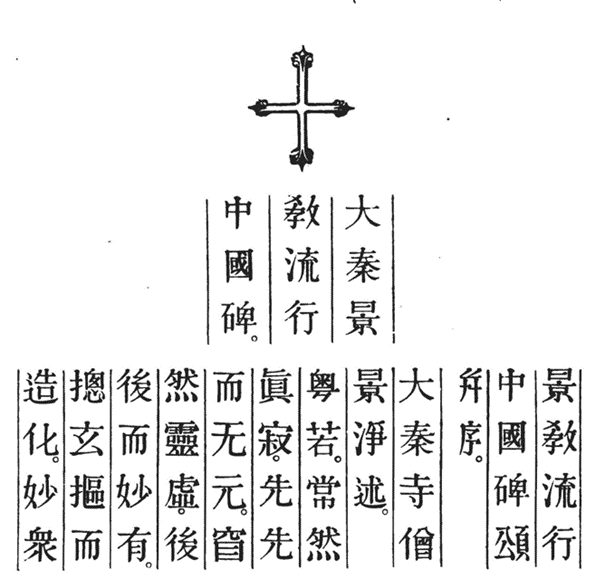
\includegraphics[width=\textwidth]{ChristologieCultureHistoire/Images/PremierParagrapheStele.png}
 
    \label{fig:my_label}
\end{figure}
 Si le livre d'Alopen 150 ans plutôt s'appelait simplement "Sûtra de Jésus-Messiah", le titre de la Stèle est le suivant :
\begin{quote}
    Monument rappelant la propagation à travers l'Empire du Milieu de l'Illustre Religion de Ta-ts'in. \cite{Havret:stelechretienne}
\end{quote}
Ta-ts'in (ou \emph{Da Qin}) indique l'Empire Gréco-Romain. Cette référence peut étonner quand on sait la répugnance des Eglises perses à être trop liées à Byzance. D'ailleurs, traditionnellement, le christianisme en Chine était appelé \textit{Bose Jiao}, l'\textit{enseignement Perse}.  En 745, il prend l'appellation officielle de religion de Da-Qin  possiblement par la chute de l'empire Sassanide perse un siècle plus tôt, qui rend caduque le terme de Perse, l'arrivée d'ambassades byzantines en Chine (attestée en 742) mais aussi par la référence à la philosophie grecque ainsi qu'à l'attribution de voyages en \textit{Da Qin} par le fondateur du Taoisme, Laozi :
\begin{quote}
    Calling Christianity the 'Religion of Da Qin' shows that the Nestorians of the Tang undeniably possessed a sensitive awareness of their political environment within China, and probably internationally as well, and moved with considerable acumen to secure the best possible position for themselves within it (\cite{Barrett:TaoismChristianity})
\end{quote}

\paragraph{Un découpage proposé en 25 sections} La stèle peut être découpée en 25 sections, la première sur les attributs de Dieu, puis les trois suivantes sur la Création et la Chute de l'homme (surtout pour développer l'idée d'un homme bon avant la chute par l'orgueil), puis les deux suivantes sur le Christ. A partir de la section 8, on trouve les caractéristiques de la religion, le baptême, les moines, l'éthique, puis plusieurs sections sur l'histoire des chrétiens en Chine, montrant une loyauté forte vis à vis des autorités politiques chinoises. Nous nous concentrerons sur les premières sections et en particulier les sections 6 et 7 proprement christologiques.  Il faut noter qu'une partie importante est liée à l'histoire du christianisme en Chine et la protection des empereurs. Cette attitude peut être mise en parallèle avec celle des premières communautés chrétiennes, avec Paul, montrant la compatibilité du christianisme avec l'Empire Romain (\cite{Baslez:MondeDevnuChretien}). 






\section{la partie proprement Christologique}

\subsection{Section 6 : l'incarnation} 

La première section qui nous intéresse parle de l'incarnation. Nous indiquerons à chaque fois les deux traductions en Français qui font foi (\cite{Havret:stelechretienne} et \cite{Pauthier:linscriptionSinganfou} \sn{la traduction de Havret est une traduction en latin et français mais la traduction française n'est pas complète - je l'ai complété à partir du texte latin}) :
 
\begin{tabular}{p{0.45\textwidth}p{0.45\textwidth}}
\\
Cependant, notre Trinité s'est comme multipliée, l'illustre et vénérable Messie, voilant et cachant son auguste majesté, se rendant tout semblable aux hommes, est venu en ce monde. les Puissances angéliques publièrent la bonne nouvelle; une femme vierge enfanta le Saint dans la grande Ts'in. Les esprits dans le Ciel annoncèrent la bonne nouvelle : "une Vierge a enfanté le Saint dans la grande Ts'in". Une étoile resplendissante a proclamé la faveur et la Perse, apercevant son éclat, vint lui faire hommage de ses présents. \cite[p. 35]{Havret:stelechretienne} & 

Ce faut alors que notre \textsc{Unité-trine} divisa sa personne dans le resplendissant et vénérable Messie, en voilant sa véritable majesté. il apparut dans le monde comme un simple mortel. Les Esprits dans le ciel annoncèrent la bonne nouvelle : "une Vierge a enfanté le Saint dans la Syrie !"  Une constellation resplendissante a proclamé l'heureux événement; les Perses ayant aperçu sa clarté, sont venus apporter leur tribut. \cite[p. 9]{Pauthier:linscriptionSinganfou} \\
                                                                                  
\end{tabular}
 
 \paragraph{Wo Sanyi, notre "trois-Un". } La pensée Taoiste utilisent le terme de Sanyi :  

\begin{quote} Le terme employé pour désigner la Trinité est un terme taoïste, \emph{sanyi} le "Trois-Un". mais pour signifier qu'il s'agissait de la Trinité Chrétienne, l'auteur de l'inscription a ajusté le caractère "\emph{Wo}" qui signifie "mon/notre". Ainsi le terme taoïste a pris un sens chrétien, "Notre Trois-Un".
    \cite[p.43]{Raguin:JesusMessieXian}
\end{quote}
Quelle est cette trinité taoïste ? Le Trois est pensé comme facteur d'harmonie entre l'Un et le Multiple permettant de «court-circuiter» la référence à Dieu ou à quelque instance supra-cosmique.\cite{Cheng:triadeChinoise}


Le terme utilisé pour le Christ est le terme syriaque de \textit{Messie}, translittéré et non traduit.

 "\textit{Voilant et cachant son auguste majesté, se rendant tout semblable aux hommes, est venu en ce monde}" est quasiment la traduction de Ph 2,6-7, soulignant l'abaissement du Christ.
 

\paragraph{Insistance sur le Ciel et l'environnement}  les cieux (\textit{constellation}) prennent une partie importante dans les deux sections sur le Christ, avec tout un passage sur l'Etoile des mages. On peut  déceler le souhait de l'auteur de montrer ce qu'est le Christ non pas en le décrivant directement comme \textit{forme},  causes ou \textit{logos} mais en insistant sur le \textit{fond},  \textit{le Ciel} qui \textit{ne s'exprime pas}. \cite[p. 109]{PolDroit:voyage} . 
\begin{quote}
    La philosophie gréco-européenne privilégie la « forme » – en grec ancien, \textit{eïdos}. Une « idée » est d’abord une « forme », qui se découpe sur un fond d’espace indifférencié. C’est ce fond d’espace qui retient l’attention chinoise, plutôt que la forme qui s’en détache. Scruter le fond plutôt que les formes, l’indifférencié plutôt que les différences, l’espace plutôt que les choses qui s’y trouvent et s’y découpent, telle pourrait être la première caractéristique de l’attitude chinoise.\cite[pp. 110-111]{PolDroit:voyage}  
\end{quote}
Dès lors, l'attitude des mages perses qui scrutent dans \textit{le Ciel} ce qui change, est finalement celle du sage Chinois. Pour le Taoisme, ce n'est pas par le discours, qui segmente et découpe mais par le biais d'histoires déroutantes, \textit{comme celle de l'étoile des mages}, que l'on peut transmettre la voie. \cite[p. 130-141]{PolDroit:voyage} 
 




\subsection{section 7 : la rédemption } 


Après l'incarnation, le texte développe en plusieurs paragraphes l'action de Jésus : 


\begin{tabular}{p{0.45\textwidth}p{0.45\textwidth}}
\\
Il accomplit les lois anciennes qu'avaient écrites les vingt-quatre Saints, direction des empires dans les conseils. Il fonda la nouvelle religion que la Trine unité, Esprit très pur, n'exprime pas au moyen de paroles, formant à la pratique des vertus par la vraie foi.  & Ainsi, s'est trouvé accompli ce que les vingt-quatre saints avaient annoncée dans l'ancienne loi : " le gouvernement des familles et des États par une grande et suprême doctrine. Il établit la doctrine pure de l'\textsc{unité-trine}, sans l'appeler une nouvelle religion. Il fortifia les bonnes habitudes par l'usage de la vraie foi. \\
\end{tabular}

\paragraph{Jésus est présenté comme un sage} Le texte insiste sur l'Esprit qui soutient la vertu sans passer par une loi (cf Jr 31,33 \sn{Jr 31,33 \textit{Je mettrai ma loi au dedans d'eux, Je l'écrirai dans leur coeur} \newline 2 Co 3,3\textit{Vous êtes manifestement une lettre de Christ, écrite, par notre ministère, non avec de l'encre, mais avec l'Esprit du Dieu vivant, non sur des tables de pierre, mais sur des tables de chair, sur les coeurs.}}  ou encore 2 Co 3,3).

Par cet  \textit{Esprit très pur, qui n'exprime pas au moyen de paroles formant à la pratique des vertus par la vraie foi}, l'auteur propose probablement une théologie accessible à la culture chinoise. pour les Chinois en effet,  ce n'est pas au moyen de raisonnements qu'on atteint le Ciel, qui s'éprouve directement
\cite[p. 117]{PolDroit:voyage} même si notre participation au Ciel en ce monde est parfois voilée.


Cependant, l'auteur ne s'arrête pas à une approche \textit{sans parole} puisqu'il mentionne les \textit{huit béatitudes} : 

\begin{tabular}{p{0.45\textwidth}p{0.45\textwidth}}
\\
Il institua les règles des huit fins, pour purifier les facultés et perfectionner les saints; il ouvrit la porte des trois principes,& Il posa les lois des huit limites morales que l'on ne doit point franchir. la poussière de la terre, purifiée comme le métal dans la fournaise, devint la vérité parfaite. Il enseigna au moindre les trois grandes vertus cardinales; 
\\ 
 en ouvrant les portes la vie et supprimant la mort. & il lui ouvrit les sources de la vie, et anéantit la mort.
\end{tabular}


 \paragraph{Référence à la Bible} Après avoir insisté sur l'éthique de Jésus, l'auteur met l'accent sur le corpus biblique, à la fois dans le registre de l'\textit{accomplissement} de l'Ancien Testament et ses 24 livres/ Saints mentionnés plus haut \sn{hors livres deutérocanoniques} que de l'annonce d'un nouveau Testament\sn{ l'auteur décompte 27 livres alors que le Corpus syriaque ne reconnaissait initialement que 22 livres (l'Apocalypse et les épîtres générales reconnus tardivement) }. 

 \paragraph{Sauver par le registre de la grâce} Face à poussière (Lieu-tch'en), expression bouddhique pour désigner les \textit{souillures de la pureté du coeur},  le texte mentionne les 8 lois morales (Pa-King, "8 circonstances"), comprises comme les Béatitudes (8 béatitudes chez Mt).  Sont aussi mentionnés la porte des trois vertus cardinales (Tch'ang), porte qui ouvre aussi à la vie et supprimant la mort (Mié-se) selon une expression chrétienne traditionnelle. 

Puis suit une expression typiquement bouddhique du soleil lumineux triomphant des porte des enfers (ti-yu) mot à mot \textit{prison de la terre} \cite[p. 49]{Havret:stelechretienne}.  Satan est ici appelé par le terme chinois \textit{Mo}, d'où la traduction de démon :

\begin{tabular}{p{0.45\textwidth}p{0.45\textwidth}}
\\
Il suspendit le soleil lumineux pour triompher de l'empire de ténèbres et {dès lors }les ruses du démons furent toutes pénétrées et déjouées
&  Il suspendit au ciel le brillant soleil de la vérité pour dissiper les habitations des ténèbres; les ruses mensongères du démon furent dès lors pénétrées et déjouées. \\
\end{tabular}



 
 
 

\begin{tabular}{p{0.45\textwidth}p{0.45\textwidth}}
\\
Conduisant à la rame la barque de la miséricorde, il s'éleva aux demeures lumineuses; dès lors quiconque possède une âme a trouvé son salut. L'oeuvre de la toute puissance étant ainsi consommée, il monta en plein midi, homme déifié.& Il mit en mouvement le navire de la miséricorde pour s'élever aux brillantes demeures; les âmes qu'il renfermait purent dès lors, en traversant le fleuve de la vie, obtenir cette fin glorieuse. A l'heure de midi, il s'éleva au séjour de la vérité. \\ Il laissait les vingt-sept livres de l'écriture, où est expliquée la grande réforme pour l'ouverture des \textit{ling-koan}
  \cite[p. 44]{Havret:stelechretienne} & 
Des saints livres ont été laissés au nombre de vingt-sept, qui ont étendu les conversions originelles en libérant les âmes.
  \cite[p. 10]{Pauthier:linscriptionSinganfou} \\
                                                                                  
\end{tabular}
 
  \paragraph{influence bouddhique du mouvement} Avec l'image de la barque de miséricorde (\emph{avalokites 'vara}), nous avons ici une belle image d'origine bouddhique, divinité plus connue en Chine sous le nom de \emph{Koan-yn} et surnommée \emph{Ta-t'se} la grande Miséricorde. D'après le bouddhisme, l'humanité tourne sans cesse comme sur une grande mer jusqu'à ce qu'elle arrive enfin au \textit{nirvana}. 
  
 % -----------------------------------------------
\section{Conséquences en terme de chemin de salut}

Quelles sont les conséquences sur le salut de cette étude rapide des deux paragraphes christologiques ?

\paragraph{Une dimension pratique du salut} Pour les chinois, la dimension pratique des débats est importante : 

\begin{quote}
    Entre ordre confucéen et contestation taoïste, il existe plus de complémentarité, malgré leurs désaccords, que d’opposition frontale. Ne perdant jamais de vue une dimension pratique, les débats chinois sont continûment traversés par des interrogations sur la bonté ou la méchanceté humaine, sur la bienveillance ou la cruauté nécessaire des souverains.

\cite[p. 147]{PolDroit:voyage}  
\end{quote}
 Regardons dans cet esprit le passage sur le mal qui précède les sections sur l'incarnation et la rédemption.
\begin{quote}
   Il arriva que Satan, disséminant ses fraudes, se para de l'ornement emprunté d'une pure essence, et qu'ouvrant une brèche dans cette grandeur morale, au milieu de cet heureux état, il y introduit la ressemblance de la confusion.
De là, des sectes aussi nombreuses que les jours de l'année, qui se suivirent pressées, et tracèrent à la suite leur sillon, tissant à l'envi les filets de leurs lois. les uns, désignant les créatures, s'appuyaient sur elles comme sur leur principe, les autres supprimant la réalité de l'Etre, se plongeaient dans la superstition, d'autres adressèrent des prières et des sacrifices pour attirer le bonheur, d'autres enfin firent parade de vertu pour en imposer aux hommes. 
\end{quote}
 
 
 Le péché introduit par Satan est décrit comme "ressemblance de la confusion". C'est un exemple de l'aspect concret du Chinois :\textit{ Tien-che }. \textit{Tien} signifie un ornement en métal; \textit{che}, chercher à paraître ce que l'on n'est pas ; se parer des dehors. La conséquence sont les \textit{sectes aussi nombreuses que les jours de l'année}; présentant les différentes voies de salut. On y a vu une critique du Taoisme (cette voie est accusé de diviniser les forces de la nature :  \textit{désignant les créatures, s'appuyaient sur elles comme leur principe}) et Bouddhisme aux tendances matérialistes et nihilistes (\textit{supprimant la réalité de l'Etre, se plongeaient dans la superstition}).  
 
 
 
 \paragraph{Par le Baptême, l'Esprit Saint nous éloigne des vaines gloires} Après la partie christologique, l'inscription développe les rites, d'abord le baptême, \textit{quittant les préoccupations vaines et mondaines pour obtenir la pureté}. Ce soucis d'humilité et de quitter le monde  rejoint la pensée du \textit{Chemin} ou \textit{Tao},  
 
 \begin{quote}
     à la fois faiblesse extrême (goutte d’eau) et puissance sans borne (océan). \ldots vent… C’est à force de faiblesse, si l’on ose dire, que le sage parvient à tant de puissance. 
\cite[p. 130 ]{PolDroit:voyage} 
 \end{quote}

Que ce soit dans la partie décrivant la chute ou au moment du baptême (et des vaines gloires), on trouve probablement une description adaptée aux oreilles chinoises, empreintes de la pensée Taoïste.

 Puis, l'auteur décrit la vie monastique : le rôle de la barbe et de la tonsure, images extérieures de la vie intérieure, l'absence d'esclave, l'égale considération de tout homme , le refus des richesses, la pratique de la générosité, le silence et la retenue. A ce titre, ils se présentent moins comme des moines bouddhiques que comme des sages pétris de sagesse confucéenne : 
 
 \begin{quote}
     Car le « mandat du Ciel », comme disent les confucéens, est présent avant tout dans le « sens de l’humanité » (ren) qui habite le cœur de chacun. Cette notion fondatrice, malaisée à définir, implique à fois, selon Confucius, d’être « juste dans le jugement », « conscient de la valeur de l’effort », « pacifique dans les conflits » et d’avoir de la « retenue ». Le \textit{ren} est ainsi l’instance de régulation des rapports entre les humains, agissant au cas par cas.

\cite[p. 122]{PolDroit:voyage}  
 \end{quote}
 Paul a préféré  l'aréopage au Temple, et les apologistes Chrétiens le terme néo-platonicien de  \textit{Logos} pour dire l'expérience du Christ et non les catégories des religions paiennes. De même, l'auteur de la \textit{Stèle} nous semble mettre en avant la sagesse confucéenne, plutôt que les moines Taoistes ou bouddhistes. Cette attention à la sagesse confucéenne explique peut être  la mention qui suit : les moines prient \textit{au secours des vivants et des défunts}, alors que la sagesse confucéenne accorde une importance forte au culte des ancêtres.
 
 

 
 
  
\paragraph{Ne pas penser séparément morale, rites privés et gestion des affaires communes} Une caractéristique importante de la civilisation chinoise est effet d’entrelacer doctrines morales, rites privés et gestion des affaires communes
\cite[p. 120]{PolDroit:voyage}. L'inscription développe non donc seulement le credo de la foi chrétienne (sections 7 et 8), mais aussi la morale et les rites (sections 9 et 10). A ces deux éléments s'ajoute la louange des empereurs chinois. Sur ce dernier point, les Chrétiens en Chine reprennent  la stratégie des chrétiens face à l'empire romain, qui s'inséraient dans le réseau de solidarité des villes par le rôle des évêques et des diacres (\cite{Baslez:MondeDevnuChretien}).


\section{Conclusion}

\paragraph{Une présentation du message Chrétien soulignant les aspects les plus accessibles à la pensée Chinoise} A travers l'étude de la Stèle, nous avons trouvé la présentation des principaux points de la Foi Chrétienne. Cependant, sans trahir le message chrétiens, l'auteur choisit une traduction qui résonne avec la culture chinoise. Au delà de la traduction, le choix des passages de la Bible comme \textit{l'Etoile dans le Ciel} ou l'accent sur certains points du rite comme la prière pour les défunts ou l'attention au \textit{Ren}, éclaire ce message chrétien de façon nouvelle. 
 
\paragraph{difficulté à penser l'acculturation religieuse} Dans nos recherches, nous avons rencontré des auteurs ne pouvant pas penser l'acculturation du message chrétien en dehors des catégories de l'hérésie. Ainsi, un article récent \cite{Gernet:Stele} s'oppose à l'interprétation d'une stèle de Xi'an acculturée à la culture chinoise et propose une clé de lecture basée sur un contexte de luttes théologiques internes au sein de l'Église nestorienne.

\begin{quote}
    rien ne prouve d'ailleurs clairement que les nestoriens aient songé à faire partager leurs croyances aux Chinois. [\ldots] Les circonstances et les mentalités étaient en effet tout à fait différentes de celle qui devait régner un millénaire plus tard, à l'époque de la contre-Réforme animée par une ambition de conquête universelle des esprits et des territoires (p. 245)
\end{quote}
Même si la communauté chrétienne qui a écrit la stèle était toujours fortement liée à l'Église perse - comme le montre les signatures de la stèle en araméen -, cette thèse nous parait difficilement acceptable à l'analyse. Les Eglises syriaques à cette époques nous sont certes assez mal connues; on peut noter l'importance du terreau judeo-chrétien à la création de ces Eglises, le milieu missionnaire parmi les marchands, la mixité culturelle, reflet des sociétés en monde iranien, la loyauté vis à vis des autorités politiques et le monachisme (\cite{Amir:CoranHistoriens}). Sans les relever tous, on retrouve de fait de nombreux éléments syriaque dans la Stèle (par exemple, influence des marchands et moines dans la création de l'Eglise de Chine), mais sans que cela ne remette en question le travail d'acculturation de la foi chrétienne en contexte chinois dont les marques sont soulignées par de nombreux sinologues. A tel point que c'est plutôt l'autre vision, celle d'une supposée trop grande acculturation qui est souvent soulignée (le P. Havret, sj note par exemple les 
\textit{    dangereux rapprochements} avec la culture Taoiste \cite[p.21]{Havret:stelechretienne}).   


Cette double polémique montre la difficulté à penser l'acculturation et sa conséquence en terme de christologie : notre vision du Christ est forcément transformée par l'acculturation, et elle peut être vécue sans être un dévoiement de la foi véritable, mais au contraire en développant des aspects du Christ qui sont restés comme en germe dans son incarnation en Judée "au temps d'Hérode" et qui peuvent se développer pleinement dans d'autres cultures et époques. 


 
\part{Christologies au défi de la culture pluraliste}
\chapter{Introduction aux Christologies au défi de la culture pluraliste}
\mn{Xavier Gué Cours ISTR 2022-2023}
\section{Synthèse du cours « Christologies et cultures dans l’histoire »}
\subsection{Prolégomènes à une réflexion sur la relation entre les christologies et les cultures et
les religions}

 \begin{Synthesis}
 Prolégomène : 
 \begin{itemize}
     \item  Un écart entre Jésus historique et la possibilité pour nous d'y accéder 
     \item un moment spécifique : la canonisation des Ecritures, reçues par la communauté. 
 \end{itemize}

 \end{Synthesis}

 
\paragraph{Passage}
 Jésus annonce le Règne de Dieu et les premiers disciples annoncent le Christ.

 \paragraph{Mystère pascal} Jésus passe d'un homme singulier au Christ qui est pour tous les hommes, qui est Un avec Dieu. A partir de ce moment là, il devient une bonne nouvelle pour tous les hommes, car il nous permet d'être uni à Dieu et avec tous les hommes.


\paragraph{Comment ?} La transmission du mystère du Christ se joue de manière \textit{vitale} (style de vie des disciples) et en même temps le discours du \textit{discours} (Christologie). Comment le discours sur Jésus va transmettre Jésus dans l'histoire : d'abord les juifs, puis le monde grec, le monde romain,... A chaque fois, des mondes très différents.

\begin{Synthesis}
    Si on affirme que Jésus est pour tous les hommes et tous les temps, il faut qu'on puisse l'annoncer et qu'il soit reçu dans tous les temps et toutes les cultures.
\end{Synthesis}


\paragraph{Christologie doit vérifier l'universalité du Christ} Vérifier : attester. En assumant la \textit{matrice de chaque culture}, le Christ se fera comprendre et recevoir. Rejoindre tous les hommes là où ils sont dans leur culture. 

\paragraph{Une partie résiste} Il s'agit de purifier la culture qui reçoit par le Christ

\paragraph{la Révélation se déploie dans l'histoire par la rencontre avec les Cultures} Tout dialogue transforme. Pas slt un développment organique dans l'histoire mais des influences qui viennent de l'extérieur de l'Eglise. Vincent de Lerins pense une vision organique de l'Eglise mais il y a un échange organique avec l'autre.

\paragraph{la rencontre avec l'autre} a pu développer des hérésies mais aussi développer une théologie féconde, de plus indispensable. 
Règle de discernement et de foi qui permet de vérifier : Calcédoine dit ce qu'on ne peut pas dire. La foi interprétant les Ecritures.

\paragraph{le Christ continue à s'incarner aujourd'hui} la parole de Dieu à s'incarner de nouveau d'une certaine manière. 
 
\subsection{Dimension historique : dans l’histoire des christologies ont émergé par la rencontre
avec des cultures}

\paragraph{Culture juive} un monde qui n'est plus notre monde. Jésus va unifier cette culture par la figure du \textbf{Messie}. cf St Pierre à la Pentecôte. La \textit{Torah} et \textit{l'espérance} sont les deux piliers de la foi juive. Le Messie était attendu. Mais aujourd'hui, est ce qu'on attend le Messie ? Messie ne veut probablement rien dire ? 

\paragraph{de l'intérêt de l'exégèse pour revenir au texte}
\begin{Ex}[Figure du Fils de l'Homme]
Pour les juifs de l'époque, rapport à Dn 7, 13-14, 
\begin{quote}
    13 Je regardais, au cours des visions de la nuit, et je voyais venir, avec les nuées du ciel, comme un \textit{Fils d’homme} ; il parvint jusqu’au Vieillard, et on le fit avancer devant lui.

14 Et il lui fut donné domination, gloire et royauté ; tous les peuples, toutes les nations et les gens de toutes langues le servirent. Sa domination est une domination éternelle, qui ne passera pas, et sa royauté, une royauté qui ne sera pas détruite.
\end{quote}
attente eschatologique (et pas directement Messie).  
\end{Ex}

\paragraph{Culture grecque} Paul rencontre le monde grec paien à Athènes, mais la plupart du temps, il s'adresse par son argumentation à des juifs grecs. 
Comment finalement parler aux grecs ? par le \textbf{logos} et de la \textbf{vérité}. Alors que pour les juifs, on est plus dans la \textit{loi} que la \textit{vérité}. L'innovation, c'est de dire que le \textit{logos s'est fait chair}.

\paragraph{Culture et monde romain} En étudiant Saint Augustin, et le problème de la \textit{religio} qui va être interprété par Lactance et Augustin, d'être relié à Dieu. Jésus va être compris comme \textit{médiateur}. Ces termes existent dans le NT mais on va les mettre en avant. 

\paragraph{Chrétienté} Comment parler du Christ dans un monde chrétien. L'idée de corps social va s'imposer, Eglise comme corps et le Christ comme la tête du Christ, et le Pape vicaire (lieutenant) du Christ. Il faudra christologiser cette idée de Roi en lui apposant le terme de \textit{serviteur}. 

\paragraph{Temps moderne} Prise de conscience en Europe d'une culture qui s'émancipe du Christianisme. Avec deux idées : 
\begin{itemize}
    \item Erasme : l'homme est au centre du monde
    \item L'Europe prend conscience qu'elle peut être moteur de l'histoire : c'est l'homme qui fait l'histoire et non Dieu.
\end{itemize}
La culture sort du Christianisme. Et donc défi pour le Christianisme d'annoncer le mystère du Christ dans cette nouvelle configuration. \textbf{le Christ comme Alpha et Omega de l'histoire, le Christ accomplit l'histoire}. On retourne à l'idée de l'eschatologie. Danielou, de Lubac, Balthazar.

\paragraph{un humanisme qui va se séculariser} L'homme qui accomplit l'humanité (Rahner). Suivre le Christ, ce n'est pas se déshumaniser, c'est s'humaniser, le mystère du Christ révèle le mystère de l'homme.


\section{La christologie au défi de la culture postmoderne et du pluralisme religieux}

 
\subsection{La remise en cause de l’optimisme de la modernité}

L'Eglise Catholique a vu que son rapport au monde avait changé. Il y avait d'autres christianisme (asiatique, arabe). Mais le Christianisme occidental avait pris le \textit{la}. 

\paragraph{On estime l'autre} depuis\textit{ Nostra Aetate}, on regarde l'autre avec estime. \textit{Ad Gentes} et l'interdiction du prosélytisme. 

 \paragraph{les chocs du XX} ont remis en cause le XX.

 \paragraph{les autres religions ne se sont pas écroulées} Au contraire, à la suite de la décolonisation, ces religions sont présentes en Europe. Sur les 18-30 ans, quasiment autant de musulmans (15\%) que de catholiques en France.

 \paragraph{Est ce que les religions sont de fait ou de droit} font elles partie du plan de Dieu ?
\begin{quote}
     « Le pluralisme et les diversités de \textbf{religion}, de couleur, de sexe, de race et de langue sont une
sage volonté divine, par laquelle Dieu a créé les êtres humains. » ? (François - Ahmad Al-
Tayyeb, \textit{La fraternité humaine}, Abou Dabi, 4 février 2019).
\end{quote}
 Ce n'est pas une punition (Babel) : on associait la diversité, à la division et au péché et ici, on l'attache à la sagesse de Dieu.

\paragraph{impact sur la Christologie} On passe dans un monde pluriel, qui resiste. Nous sommes passés de la modernité vers la postmodernité.

\paragraph{C'est quoi la post-modernité ? }
 
\subsection{La culture postmoderne et le pluralisme religieux}

\paragraph{la modernité} le grand récit de la modernité, l'homme se fait tout puissant \textit{à l'image de Dieu}. L'homme participe à la puissance divine.

 
   \begin{quote}
    « C’est\mn{ Rémi Brague, \textit{Le règne de l’homme}. Genèse et échec du projet moderne, Paris, Gallimard, (4ème de couverture).
2015 : } à l’époque moderne que l’homme en est arrivé à se dire le créateur de sa propre
humanité. Autrefois, il se croyait l’oeuvre de la nature ou l’enfant de Dieu. Désormais, il
entend conquérir l’une et s’affranchir de l’autre. Il veut rompre avec le passé, se donner
souverainement sa loi, définir ce qui doit être, dominer. Telle est l’ambition vertigineuse que
raconte cet ouvrage »
\end{quote} 
 
\paragraph{séparation} entre la culture et le religieux. 

\paragraph{Opposition de l'Eglise à cette sortie de la culture}
    Pie IX, dans le syballus (1864), condamnait toute une série d’affirmations dont la dernière :
\begin{quote}

« Le pontife romain peut et doit se réconcilier et composer avec le progrès, le libéralisme et la
culture moderne » (DS 2980). 
\end{quote}


\paragraph{Rupture et continuité de la post modernité par rapport à la modernité} On va critiquer la modernité au nom de la déconstruction des grands récits, y compris celui de la modernité. On arrive à une relativisation, \textit{fragmentation}. 

\paragraph{Il n'y a plus de grands récits, de mythes collectifs}

\paragraph{Neutralité de l'Etat} à la différence de \textit{Cujus Regio Cujus Religio}, ici avec l'Etat laic, diversité religieuse voire culturelle, fragmentation de la vérité. Des cultures qui se confrontent.  La seule unité est le marché, le reste est fragmenté.
\begin{Ex}[Ecologie, dernière utopie]
    Ecologie, un peu ambigue, car un récit par la peur. 
\end{Ex}

\subsection{Un monde déculturé}

\begin{quote}
    Olivier Roy, l'aplatissement du monde, 2022
    Toute culture renvoie à un système d'imaginaires qui fait sens. Un implicite partagé par toute une population. Il note qu'il y a une crise des imaginaires comme la crise des idéologies. 
\end{quote}
 Le politique n'est plus porté par la culture mais par le \textit{contrat}. 

 \paragraph{Les grands récits sont aux mains des radicaux} Sans imaginaire commun, difficile de se projeter dans l'avenir. 

 \paragraph{L'écologie, par un imaginaire mais un } mobilise les jeunes. 

\paragraph{Le marché n'a à faire qu'avec des individus} mais doit lutter contre la culture, les religions : "cela complique tout". On doit supprimer les frontières (globish : langue qui n'est plus culturel mais qui est une langue d'échange).

\paragraph{S'il n'y a plus de cultures, il faut des normes} On est dans l'explicite et pas l'implicite. Ce système normatif doit s'imposer à eux. La pédagogie authoritaire suppose que l'on part d'une \textit{table rase}. \textbf{Epoque de déculturation}.
 
\subsection{Deux principes « unificateurs » de la postmodernité}

\paragraph{Du débat au \textit{dialogue}} Aujourd'hui, il faut apprendre à dialoguer. \mn{cf Synode sur la Synodalité}. L'unité ne peut s'imposer par en haut. Mais on n'a pas la culture du dialogue. On construit notre unité par le dialogue. Il faut passer d'une culture libérale à un imaginaire nourri par le dialogue. 

\paragraph{de l'efficacité à la fécondité} L'unité se fait sur ce qui \textit{marche}. Même si le progrès est remis en cause, on n'est pas loin de la modernité. 
Hannah Arendt : 
\begin{quote}
    on est passé de la vérité au "cela marche".
\end{quote}
\begin{quote}
    « La vérité dont il s’agit dorénavant, c’est celle de ‘l’opérationnel’ (ce qui est faisable : Marchbarkeit). Autrement dit, la vérité à rechercher ne se trouve pas dans l’être ni même dans les événements antérieurs, mais dans la transformation du monde, dans l’organisation du monde ; c’est la vérité qui se rapporte à l’avenir et à l’action » (Ratzinger, La foi chrétienne
hier et aujourd’hui, 25).
\end{quote}
Il faut une vérité \textit{applicable}. 
\begin{quote}
    Paul VI (Evangeli nuntiandi 1975) : « L’homme contemporain écoute plus volontiers les
témoins que les maîtres — disions-Nous récemment à un groupe de laïcs — ou s’il écoute les
maîtres, c’est parce qu’ils sont des témoins ”. »
\end{quote}
Le témoin, c'est celui qui montre que le discours marche dans sa vie. 

Mais l'efficacité (cela marche) ne prend pas en compte le temps. Passer à la fécondité : ce qui porte du fruit par opposition à ce qui est stérile. Il faut viser une certaine fécondité aujourd'hui. 

\begin{Ex}[Eglises africaines]
    marchent car elles proposent la guérison. 
    Approche néanmoins souvent trop individualisme

    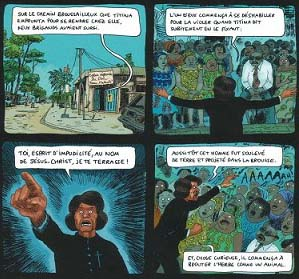
\includegraphics[width=0.7\textwidth]{ChristologiePluraliste/Images/Aya.jpg}
\end{Ex}

\subsection{La christologie à l’épreuve du dialogue}

\paragraph{Remet en cause le Christ comme le tout} Elle reinterpréte la différence entre contingent et absolu, Jésus et le Christ. On a bcp insisté sur \textit{Jésus et l'unique}. Si on annonce Jésus absolu, on ne peut entrer en dialogue. Il convient donc de se reposer la question de décentrer \textit{Jésus} par rapport à \textit{Dieu}. 

\paragraph{comment annoncer le Christ de manière dialogale et rassembler les hommes} question pas simple 
\begin{quote}
    Mgr Ladaria dans la présentation du document de la CTI (dont il est le secrétaire)
Christianisme et les religions 1996 écrit : « En contraste avec l’intention et la lettre même des textes conciliaires, un certain relativisme religieux s’est développé dans certains milieux au cours des années postconciliaires, comme si toutes les religions étaient d’égale valeur pour obtenir le salut; on perdit ainsi grandement le zèle missionnaire, et même la médiation unique
et universelle du Christ fut mise en doute. »
\end{quote}



\subsection{La christologie au défi de la fécondité sociale} 


\paragraph{fécondité} Les fruits de Sainteté. 
\begin{quote}
    Voir les critères de vérité de la Révélation : le GRIC : GROUPE DE RECHERCHE
ISLAMO-CHRETIEN (GRIC), « L’Ecriture des uns vue par la foi des autres », Ces Ecritures
qui nous questionnent, la Bible et le Coran, Le Centurion, Paris, 1987, p. 71-139 (chapitre 3 ).
Outre le contenu du message (du Coran), le Gric propose le critère de la fécondité du message
pour juger de l’authenticité de la révélation coranique. « L’autre critère (…) est celui de la
fécondité du message parmi les hommes (…). On doit donc pouvoir reconnaître dans la vie
individuelle et collective des hommes d’hier et d’aujourd’hui l’influence du message ; ce
qu’on pourrait appeler des fruits de sainteté » (p.103).
\end{quote}

\paragraph{Christologie} dans cette perspective. Quel image d'un Christ qui transforme notre société ? \textbf{des christo-praxies}. Certains auteurs montrent que le Christ doit inspirer notre agir et susciter la fraternité entre nous. Si elle nous enferme sur nous mêmes, il y a un problème.


\section{Plan, bibliographie et déroulement du cours}
\subsection{Plan}
 
\subsection{Bibliographie}
 
\subsection{Déroulement}


 \section{Texte}











 


\chapter{De Jésus au Christ}

\section{Eléments bibliographiques}
\begin{itemize}
    \item HARNACK, A., L’essence du christianisme, tr. par J.-M. TÉTAZ, Genève 2015.
    \item HAZARD, P., La crise de conscience européenne 1680-1715, Paris 1961.
    \item LESSING, G. – REIMARUS, Fragments d’un anonyme de Wolfenbüttel, tr. par M. GÉRAUD,
Paris 2018.
    \item REYMOND, B., A la découverte de Schleiermacher, Paris 2008.
    \item SCHLEIERMACHER, F., Discours sur la religion à ceux de ses contempteurs qui sont des
esprits cultivés, tr. par I. J. ROUGE, Paris 1944
    \item ID., La cohérence de la foi chrétienne, tr. par B. REYMOND, Genève 2018.
    \item SCHWEITZER, A., « Histoire des recherches sur la vie de Jésus. Considération finale », ETR
69 (1994) 153-164 (tr. par J-P. SORG).
\end{itemize}

%--------------------------------------- 
\section{Introduction}

\paragraph{Une culture de dialogue, c'est accepter de se remettre en cause} Sinon, on est dans une \textit{apologie}, une \textit{dispute}. 

\paragraph{Comment comprendre le dogme ?} \textit{Si Jésus est vrai Dieu}, où on accepte ou on accepte pas.  Aussi, il ne faut pas partir du dogme mais les conditions actuelles nous obligent à repartir de Jésus et l'histoire de Jésus comme un lieu de débat. \textit{Qui dites-vous que je suis}. Le recevoir dans le dialogue.

\paragraph{le dogme au service de la parole de Dieu}

\paragraph{Approche du cours, ne pas partir du dogme mais du dialogue sur la personne de Jésus} Dans le XIX, un dialogue entre la culture chrétienne et la culture des lumières : 
\begin{itemize}
    \item Pour sortir du dilemne entre \textit{dogmatisme} et du \textit{rationalisme} (Jésus comme maître de moral), il fallait revenir à l'histoire de Jésus et montrer que Jésus est la source du Christianisme.

    \item Or ce retour à l'histoire concrête (à l'homme Jésus), conduit à une certaine relativisation : \textit{Jésus n'est pas l'unique}
\end{itemize}





%--------------------------------------- 
\section{La remise en cause historique de la foi en Christ}

\paragraph{Approche théologique} C'est toujours intéressant de ne pas affronter la question directement en théologie. Ici, l'astuce du chemin est de montrer comment le \textit{débat} a eu lieu.


\subsection{Le mouvement unitarien à l’origine de la crise du dogme christologique}

\begin{Def}[Unitarien]
mouvement anti-trinitaire, qui insiste sur l'unité de Dieu, qui part d'Italie au XVI. Ils vont en Pologne, Grande Bretagne (Newton) et USA (Jefferson, Dickens).
\end{Def}
On l'appelle aussi le \textit{socinianisme}, de Sozzini (1539-1604). 
Ils vont au delà de la Réforme : 

\begin{quote}
    « Quand au Christ, s’il est fils de Dieu il n’a pas la nature divine, “car cela n’est pas seulement contraire à la droite raison, mais c’est aussi contraire à la Sainte Écriture » (Catéchisme de Rakow, question 72).
\end{quote}

Jésus intercède pour l'homme et il n'est donc pas Dieu. A la différence d'Arius qui considérait Jésus comme première des créatures de Dieu et non pas un homme, ici, Jésus est homme. On fait appel à la raison et l'écriture.

\paragraph{Il fallut répondre à ces unitarien} en repartant des Ecritures.




\subsection{La critique des traditions et des dogmes : la Renaissance et les Lumières} 


\paragraph{La Renaissance revient aux sources} avec l'humanisme (Erasme) et Luther (qui revient aux Ecritures). L'idée est que \textit{l'eau est plus pure à la source}. On remet en cause les traditions entassées.

\paragraph{Les Lumières vont valoriser l'autonomie de la Raison} au lieu de s'appuyer sur l'autorité des autres. Doute méthodique de Descartes.  De plus en plus, on va invoquer les Ecritures contre les dogmes.


\paragraph{L'Ecriture va elle même être fragilisée} Richard Simon, Oratorien (1711) publie \textit{l'histoire critique du vieux testament} (1630). Il s'aperçoit qu'il y a des problèmes, en particulier que Moise ne pouvait avoir écrit le Pentateuque. 





\subsection{La crise du principe scripturaire}  
\paragraph{Question herméneutique au dépend de l'autorité} Chez les catholiques, le magistère.  Mais les protestants, problème du critère (Luther dit : \textit{la Foi sauve}). 

\subsection{La rupture entre la vérité universelle et la révélation historique}  
\paragraph{XVIII : siècle de la Loi} ce qui est stable, découverte avec Newton des lois qui gouvernent le monde. on a du mal à penser l'intervention de Dieu dans le monde. 

\paragraph{Signification universelle de Jésus est posée} Lessing oppose une vérité universelle à un événement historique : 

\begin{quote}
   « Des vérités historiques accidentelles ne peuvent jamais devenir la preuve de vérités rationnelles nécessaires » (Lessing, Über den Beweis des Geistes und der Kraft, 1777). 
\end{quote}

Les vérités sur Dieu sont inaccessibles à un événement historique, fut il Jésus. E. Kant dira que \textit{Jésus c'est celui qui a incarné les valeurs mais quand on a la loi morale, on n'a plus besoin de lui}.

\subsection{La thèse de Reimarus et l’aboutissement christologique de la crise} 

\paragraph{Reimarus pousse à l'extrême} Il est publié à titre postume, avec une intention radicale entre Jésus et les apôtres. 
\mn{LESSING, G. – REIMARUS, Fragments d’un anonyme de Wolfenbüttel, tr. par M. GÉRAUD, Paris 2018.}

A partir de là, il va expliquer ce qui s'est passé (ce sont les apôtres qui fondent le christianisme). Rupture maximale entre Jésus et le Christ de la Foi.

\begin{quote}
    « J’ai montré jusque-là que le nouveau système modifié des apôtres, celui d’un libérateur spirituel souffrant qui doit ressusciter de la mort et après son Ascension au ciel reviendra bientôt du ciel avec une grande force et dans une grande gloire, est inventée et fausse dans son premier fondement essentiel, à savoir la résurrection d’entre les morts : 1) parce que le témoignage prétendument extérieur de la garde romaine, chez Mathieu, est en soi souverainement absurde, et n’est jamais mentionné par aucun des autres évangélistes et apôtres, mais que ce système est contredit par nombre de circonstances, si bien qu’il reste plutôt tout à fait possible et fort vraisemblable (…) que les disciples de Jésus étaient venus la nuit, avaient volé le cadavre et dit ensuite qu’il avait ressuscité ; 2) parce que les disciples de Jésus eux-mêmes, comme témoins de la résurrection, non seulement varient beaucoup sur les points principaux de leur déclaration, mais encore se contredisent aussi entre eux de plusieurs manières, clairement et grossièrement (…) (Reimarus, 105).
\end{quote}


\begin{quote}
    (…) Il ne pouvait manquer que quelques Juifs qui compilaient les différentes descriptions, en viennent à penser que leur Messie viendrait deux fois, et ce sous une forme radicalement différente. On conçoit donc avec évidence que les apôtres se servirent désormais de ce système, bien que peu l’aient adopté, car leur premier système, goûté par la plupart, était réfuté par son issue ; et qu’ils se sont donc aussi promis de Jésus, comme étant le Messie, après sa mort, une autre venue glorieuse. Il faut en outre savoir que les Juifs pensent que la résurrection des morts suivrait l’autre venue du Messie, qui à ce moment jugerait les morts et les vivants : et alors commencerait le royaume des cieux ou l’autre monde (…). Les apôtres devaient donc eux aussi, grâce à leur nouveau système, promettre une autre venue du Christ dans les nuées du ciel, où ce qu’ils avaient maintenant espéré en vain serait exaucé, et où ses adeptes croyants, une fois le tribunal passé, devaient hériter du royaume » (Reimarus, 107).
\end{quote}
%--------------------------------------- 
\section{Retrouver la signification universelle de Jésus}

\paragraph{Comment refaire le lien ? }


\subsection{Schleiermacher : le Christ romantique}  

\paragraph{Courant libéral } au début du XIX. : courant libre par rapport au dogme et le discuter par rapport à la modernité. \textit{Annoncer la Foi dans la culture de l'époque}, c'est prendre des risques, entre répéter et personne ne comprend ou bien s'adapter trop à la culture.

\paragraph{F. Schleiermacher} plus grand théologien du XIX. \textit{Le Christ romantique}. Il est passé par les \textit{frères moraves} (équivalent des charismatiques). En 1799,  il publie le \textit{Discours sur la religion à ceux de ses contempteurs qui sont des esprits cultivés}.
\mn{SCHLEIERMACHER, F., Discours sur la religion à ceux de ses contempteurs qui sont des esprits cultivés, tr. par I. J. ROUGE, Paris 1944}

Il ouvre une nouvelle voie en montrant que l'\textit{homme est essentiellement religieux}. Figure concrète de Jésus et le Christ pour tous les hommes.

\paragraph{L’idée de « sentiment » (Das Gefühl)} Il refuse la métaphysique classique et de l'autre côté la morale (de Kant). Ce qui est premier, c'est l'experience d'une \textit{dépendance radicale avec le divin}. A partir de cette expérience fondamentale, il s'agit de donner des mots à cette expérience spirituelles. Le langage religieux provient de cette expérience mais ne peut l'enfermer.

\begin{Prop}
Est ce que l'expérience mystique est première ou bien est ce que le langage religieux permet de comprendre l'expérience mystique ? 
\end{Prop}

\paragraph{La conscience divine en Jésus} Il y a une conscience divine en Jésus, transparence en Jésus, immédiateté (proximité de Dieu, du Royaume de Dieu).
En Jésus, son humanité possède la capacité de communiquer son expérience aux autres.



\paragraph{Le Christ médiateur et rédempteur} Jésus va révéler à tous les hommes cette dépendance absolue envers Dieu. Un impact collectif sur les hommes, \textit{contagion de son expérience}. 
\begin{Ex}
Quelqu'un qui est lumineux, charismatique, irradie autour de lui, ces disciples deviennent aussi lumineux.
\end{Ex}

\paragraph{le Christ devient le sommet de l'expérience religieuse} Il a eu la foi parfaite et il transmet son expérience. Mais on n'a pas de foi en Jésus, pour Schleiermacher.

Pour la question de la rédemption, la croix n'est pas essentiel pour Schleiermacher. Le Rédempteur c'est celui qui nous met en communication avec Dieu. 





\begin{quote}
    « Il doit, après chacune de ses excursions dans l’Infini, \textit{extérioriser l’impression qu’il en rapporte, de façon à faire d’elle ainsi un objet communicable par l’image ou la parole} (…) et il doit donc aussi, involontairement et pour ainsi dire dans l’état d’enthousiasme\sn{habité par Dieu} (…) figurer pour autrui ce qui lui est arrivé, sous une forme sensible, en poète ou en voyant, en orateur ou en artiste. Un tel homme est un véritable prêtre du Très-Haut, qu’il rend plus accessible à ceux qui ne sont pas habitués à saisir que le fini et sa valeur minime ; il leur présente les choses célestes et éternelles comme des objets de jouissance et de communion, comme la seule source inépuisable de ce vers quoi tend toute leur aspiration supérieure. Il vise ainsi à éveiller le germe somnolent de la meilleure humanité, à allumer l’amour du Très-Haut, à transformer la vie ordinaire en une vie plus haute, à réconcilier les fils de la terre avec le ciel\sn{Ici la rédemption} (…) C’est ici la prêtrise supérieure, celle qui fait connaître l’âme intime de tous les mystères spirituels, et dont la voix descend des hauteurs du royaume de Dieu » (Schleiermacher, Discours, 125-126).
\end{quote}





\paragraph{Les ambiguïtés de la pensée de Schleiermacher} 


\paragraph{Reprend le dogme de Chalcédoine} ce qui fait dire que certains théologiens disent qu'il est tout à fait orthodoxe.

\begin{quote}
    « Quand je considère, dans les descriptions tronquées de sa vie, la sainte figure de celui qui est le sublime auteur de ce qu’il y a jusqu’ici de plus magnifique dans la religion, ce que j’admire ce n’est pas la pureté de sa doctrine morale ; celle-ci n’a fait après tout qu’exprimer ce que tous les hommes parvenus à la conscience de leur nature spirituelle ont de commun avec lui, et à quoi ne peuvent ajouter une plus grande valeur ni le fait de l’exprimer, ni celui d’être le premier à l’exprimer (…). Tout cela n’est que choses humaines. Mais ce qui est véritablement divin, {c’est la magnifique clarté qu’a revêtue dans son âme la grande idée qu’il était venu représenter, l’idée que tout ce qui est fini a besoin, pour sa liaison avec la Divinité, de médiations supérieures.} (…) Considérons seulement la vivante intuition de l’Univers\sn{ie Dieu}, qui remplissait toute son âme, sous la forme parfaite sous laquelle nous la trouvons en lui. Si tout fini, pour ne pas s’éloigner toujours plus de l’Univers et ne pas aller s’éparpillant dans le vide et le néant, pour maintenir sa liaison avec le Tout et s’élever à la conscience de cette liaison, a besoin de la médiation d’un élément supérieur, s’il en est ainsi, cet élément médiateur, qui ne doit pas avoir lui-même à son tour besoin d’une médiation, ne peut absolument pas n’être que fini ; \textbf{il doit appartenir aux deux règnes : il doit participer de la nature divine de même et dans le même sens qu’il participe de la nature finie.} Or, que voyait-il autour de lui qui ne fût fini et soumis au besoin de la médiation ? Et où se trouvait un principe de médiation en dehors de Lui ? Personne ne connaît le Père que le Fils, et celui auquel Il veut le révéler. Cette conscience du caractère unique de sa religiosité, du caractère primordial de sa conception, et de sa force dont celle-ci était douée pour se communiquer et susciter de la religion, a été chez lui à la fois la conscience et de sa fonction médiatrice et de sa divinité » (Schleiermacher, Discours, 316-317).
\end{quote}

\paragraph{Jésus n'est pas un médiateur exclusif pour Schleiermacher} Il ouvre l'idée que la figure du médiateur dépasse la figure historique de Jésus. Médiateur \textit{par excellence} mais non unique.

\begin{quote}
    « Avec cette foi en lui-même, qui peut s’étonner qu’il ait été certain non seulement d’être le médiateur pour beaucoup d’êtres, mais encore de laisser derrière lui une grande école, qui déduirait de sa religion à Lui sa religion à elle, toute semblable (…). Mais \textbf{il n’a jamais affirmé être l’unique objet} de l’application de son idée, être le seul médiateur, et il n’a jamais confondu son école avec sa religion. (…) Aujourd’hui encore il devrait en être ainsi : celui qui pose cette même intuition comme base de sa religion est un chrétien, sans considération d’école, qu’il déduise historiquement sa religion de lui-même ou de n’importe qui d’autre. Le Christ n’a jamais donné les intuitions et les sentiments qu’il pouvait communiquer lui-même comme contenant tout ce que devait embrasser la religion qui devait sortir de son intuition fondamentale ; il a toujours engagé à tenir compte de la vérité qui viendrait après lui » (Discours, 318-319).
\end{quote}

\subsection{La christologie libérale de A. von Harnack (1851-1930)}  
\paragraph{L’essence du christianisme} 
Publication de son cours à Humbold à tous les étudiants de Humbold (Berlin).  
\mn{HARNACK, A. (von), L’Essence du christianisme, tr. par J.-M. TÉTAZ, Genève 2015.
}
On ne peut réduire l'essence du Christianisme aux Evangiles mais aussi à toute l'influence qu'il a eu par la suite. Il faut prendre toute l'histoire. \textit{Pour connaître Jésus, il faut regarder les chrétiens aujourd'hui}.
Plus une personnalité est impressionnante, plus il \textit{impressionne} d'autres et donc c'est en voyant comment les autres ont été touchés, qu'on peut accéder à l'essence de cette personnalité.



\begin{quote}
    « Toute grande personnalité influente ne révèle une partie de son essence qu’en ceux sur lesquels elle agit. On peut même dire que plus une personnalité est impressionnante et plus elle intervient dans la vie intérieure d’autres personnes, moins il possible de reconnaître la
totalité de son essence à ses seules paroles et ses seuls faits et gestes (…) Des forces ont été libérées non une seule fois, mais toujours à nouveau, alors nous devons aussi prendre en compte toutes les productions ultérieures de son esprit. Car ce n’est pas d’une d’ ‘doctrine’ qu’il s’agit, qui aurait été transmise et répétée de façon monotone, ou modifiée arbitrairement, mais bien d’une vie qui, toujours ranimée, brûle de son propre feu » (Harnack, L’essence, 93- 94).
\end{quote}


{Discerner le Christ dans la vie : image du noyau du fruit} Il faut dépouiller le fruit. 

\begin{quote}
    « Dans la prédication de Jésus à propos du Royaume de Dieu, (l’historien) doit séparer ce qui est propre de ce qui est transmis, le noyau de l’écorce (…). Le Royaume de Dieu vient lorsqu’il vient vers les individus, lorsqu’il pénètre dans leur âme et en prend possession. Le Royaume de Dieu est certes domination de Dieu – mais c’est la domination du Dieu saint dans les cœurs des individus, c’est Dieu lui-même avec sa force. Tout drame au sens extérieur du monde, au sens de l’histoire du monde, a disparu ; tout ce qui concernait une expérience future extérieure a été englouti » (Harnack, L’essence, 122).
\end{quote}
\paragraph{La prédication de Jésus} On peut résumer en (p.119):
\begin{itemize}
    \item Le Royaume de Dieu et sa venue
    \item Dieu le Père et la valeur infinie de l’âme humaine
    \item La justice supérieure et le commandement d’amour
\end{itemize}


\paragraph{Le Royaume de Dieu et sa venue} Non pas un royaume exterieur mais un royaume intérieur et individualiste. Il ne s'agit pas de trouver le Règne (pas de dimension sociale). Ce Royaume vient vers les personnes humiliées.




\paragraph{Dieu le Père et la valeur infinie de l’âme humaine}  filiation divine ("inscrit au ciel", "cheveux par terre"). Le Père est la providence : 

\begin{quote}
    « Qui a le droit de dire ‘mon Père’ à l’être qui régit le Ciel et la Terre est lui-même élevé au- dessus du Ciel et de la Terre et possède une valeur qui est plus haute que tout le mystère du monde » (Harnack, L’essence, 129).
\end{quote}

Il ne fait pas la différence entre Jésus et Père et les disciples. L'âme a donc une valeur infinie quand elle se tourne vers Dieu car elle devient "fils bien-aimé". La filiation entre Dieu et Jésus, \textit{unique} et la notre, \textit{adoptive} n'est pas différenciée ici.




\paragraph{La justice supérieure et le commandement d’amour}  

\begin{quote}
    « L’amour du prochain est sur terre la seule façon de mettre en œuvre l’amour de Dieu qui vit dans l’humilité » (Harnack, L’essence, 134).
\end{quote}
Il essaye de dire l'essentiel, le reste est ajouté.

\paragraph{La christologie}   Que devient la christologie ? Quelle auto-compréhension de Jésus ? Pour Harnack, il s'agit uniquement de "garder ses commandements". \textit{Décentrement} de Jésus qui renvoie les disciples au Père. Il va conclure que : 
\begin{quote}
    « Sa conscience d’être le Fils de Dieu n’est donc rien d’autre que la conséquence pratique de la connaissance de Dieu comme le Père et comme son Père (…). Jésus est persuadé de connaître Dieu comme personne ne l’a connu avant lui ; et il sait qu’il a la vocation de communiquer à tous les autres en parole et en acte cette connaissance de Dieu – et donc la filialité divine. » (Harnack, L’essence, 169).
\end{quote}

On retourne ici à Schleiermacher : nous participons comme Jésus, au même niveau que lui.  

Il est en deçà d'une dogmatique classique : 
\begin{quote}
    « Combien s’éloigne-t-on alors de ses idées et des prescriptions lorsqu’on fait précéder l’Evangile d’une confession ‘christologique’ et qu’on enseigne qu’il faut d’abord avoir des idées correctes sur le Christ avant de pouvoir venir à l’Evangile ! C’est inverser l’ordre des choses. On ne peut avoir des idées et des doctrines ‘correctes’ sur le Christ que dans la mesure où l’on a commencé à vivre conformément à son Evangile » (Harnack, L’essence, 181).
\end{quote}

Critique assez forte de la dogmatique.


\subsection{La figure « libérale » de Jésus dissoute par la question eschatologique}  

\paragraph{Découverte récente et renforcement de l'eschatologie} Jésus ne croyait pas à un royaume intérieur :

\begin{quote}
    « Le Jésus de Nazareth, qui vint comme un Messie, qui annonça la moralité du royaume de Dieu, qui fonda le royaume des cieux sur la terre et qui mourut afin de consacrer son œuvre, n’a jamais existé. C’est une figure qui a été esquissée par le rationalisme, rendue vivant par le libéralisme et habillée historiquement par la théologie moderne » (A. \textsc{Schweitzer}, Geschichte der Leben-Jesu-Forschung, 620.)
\end{quote}
%--------------------------------------- 
\section{Conclusion}






 

\chapter{De Jésus au Christ - 2}
\mn{31/1/23}
\section{Eléments bibliographiques}
\begin{itemize}
    \item CHÉNO, R., Dieu au pluriel. Penser les religions, Paris 2017.
    \item COMMISSION THEOLOGIQUE INTERNATIONALE, Le christianisme et les religions, Rome
1997.
    \item DALFERTH, I. U., « Inkarnation : Der Mythos vom inkarnierten Gott » dans Der auferweckte
Gekreuzigte, Tübingen 1994, 1-37.
    \item DUPUIS, J., Vers une théologie chrétienne du pluralisme religieux, tr. par O. PARACHINI,
Paris 1997.
  \item HICK, J., The Myth of God Incarnate, Londres 1977.
  \item KNITTER, P. F., No Other Name ? A Critical Survey of Christian Attitudes Toward the World
Religions, Maryknoll 1985.
  \item KNITTER, P. F., « La théologie catholique des religions à la croisée des chemins », Concilium
203 (1986) 129-138CHÉNO, R., Dieu au pluriel. Penser les religions, Paris 2017.
  \item COMMISSION THEOLOGIQUE INTERNATIONALE, Le christianisme et les religions, Rome
1997.
  \item DALFERTH, I. U., « Inkarnation : Der Mythos vom inkarnierten Gott » dans Der auferweckte
Gekreuzigte, Tübingen 1994, 1-37.
  \item DUPUIS, J., Vers une théologie chrétienne du pluralisme religieux, tr. par O. PARACHINI,
Paris 1997.
  \item HICK, J., The Myth of God Incarnate, Londres 1977.
  \item KNITTER, P. F., No Other Name ? A Critical Survey of Christian Attitudes Toward the World
Religions, Maryknoll 1985.
  \item KNITTER, P. F., « La théologie catholique des religions à la croisée des chemins », Concilium
203 (1986) 129-138
\end{itemize}

%--------------------------------------- 
\section{Introduction}

Un certain nombre de chrétiens ont voulu renouvelé le christianisme à partir de l'histoire. 

Shleiermacher :  Comment finalement des personnes charismatiques peuvent avoir de l'influence ? Mais pas limité au Christ.
Harnack : A partir du moment où l'homme vit de la relation à Dieu, il est messie.
\begin{marginfigure}
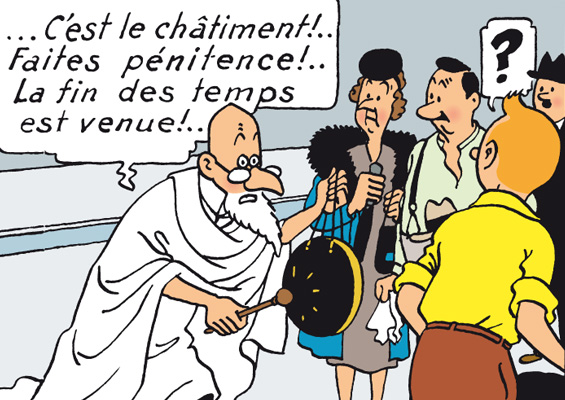
\includegraphics[width=\textwidth]{ChristologiePluraliste/Images/TintinFindesTemps.jpg}
\caption{La figure Charismatique peut être un soucis ...}

\end{marginfigure}



%--------------------------------------- 
\section{L’émergence de la théologie du pluralisme religieux}

\begin{Def}[théologie du pluralisme religieux]
modèle du paradigme : à l'image des sciences, on évolue de paradigme en paradigme
\end{Def}

\begin{Ex}
On passe du paradigme ptomélique, à Newton puis relativité.
\end{Ex}

D'après Kuhn, \href{https://fr.wikipedia.org/wiki/La_Structure_des_r%C3%A9volutions_scientifiques}{La Structure des révolutions scientifiques} \mn{intéressant à lire}



%--------------------------------------- 
\subsection{La théorie des trois paradigmes}
  Quel paradigme : 
\begin{itemize}
    \item Vision Exclusiviste, ecclesiocentriste : Le salut pas possible hors de l'Eglise. K. Barth, courant évangéliste actuel (Manille, 1986, "rien ne permet de dire que le salut peut s'obtenir en dehors du Christ confessé explicitement"). \textit{Concile de Florence} au XVI. \textit{Hors de l'Eglise point de salut. }
    \item Vision Inclusiviste, christocentrisme. Au XX. Pas un seul chemin pour aller au Christ.
\item vision théocentrique ou pluraliste. Plusieurs voix pour aller à Dieu
    
\end{itemize}

%--------------------------------------- 
\subsection{Le promoteur du « pluralisme » : J. Hick}

 \paragraph{John Hicks - 2012} D'abord évangélique puis protestantisme libéral après l'Inde. Double conversion. 

%--------------------------------------- 
\subsection{Qui est Paul F. Knitter ?}
 
\paragraph{F. Knitter} Catholique, Chicago, 1966 Rome. Cincinnati. 

1985 : \textit{No Other Name ? } Actes : pas d'autre nom pour être sauvé 


%--------------------------------------- 
\section{La christologie de Knitter : L’unicité relationnelle de Jésus}


\paragraph{Question} comment Jésus est il unique ? 

\paragraph{Histoire} Comment ce Jésus crédible il y a deux mille ans, est il toujours crédible aujourd'hui ? Ce rapport à l'histoire est spécifique aux Occidentaux. Histoire avec un progrès.

\paragraph{Ces approches empêchent le vrai dialogue avec les autres religions} Il faut accepter être impacter à l'autre. Sinon, ce n'est pas un dialogue. Soutient le modèle théocentrique. Jésus : unique mais sans absorber les autre figures prophétiques. 


\paragraph{part des textes bibliques} en même temps historique et théologique


\paragraph{se met à la place des premiers disciples de Jésus} Aspect historique au service de la théologie

%--------------------------------------- 
\section{L’unicité relationnelle de Jésus et la christologie du NT}
%--------------------------------------- 
\subsection{Jésus était théocentrique}
 
 
\paragraph{Jésus est théocentrique} au XX, Jésus annonce le \textit{Royaume de Dieu} : il ne s'annonce pas lui-même. 
Jésus est centré sur le Père. Il est \textit{Regno-centrique} (proche du théocentrisme). 

%--------------------------------------- 
\subsection{Du royaume de Dieu au Fils de Dieu}

 \paragraph{transformation du message du Christ à sa mort}
Dans le NT, il y a un message Christocentrique. Jn 20;28 : "mon Seigneur et mon Dieu". Il y a dejà une subordination du Christ au Père. On pense parfois trop la distinction en pensant au concile de Nicée. 

\paragraph{Jésus aurait fait une expérience de Dieu au début de sa mission} mais cela ne dit pas une exclusivité mais une mission unique. Il s'est pensé le prophète eschatologique de la fin des temps ?  

\paragraph{Loisy} mettait le doigt sur un problème. Expérience de salut faite par ses chrétiens. Les chrétiens ont rencontré Jésus, à la base de cette expérience. 

%--------------------------------------- 
\subsection{La christologie est, depuis le début, dialogique, pluriforme et évolutive.}




 \paragraph{De la diversité des christologies à l’unité de la christologie}
 \paragraph{Revenir à la diversité des christologies}
4 visions de christologie par les chrétiens :

\subparagraph{Christologie Marana tha} contexte apocalytique, jésus vient juger à la fin du temps. Jésus est Seigneur (Mar).
\paragraph{Jésus divin} il est divin dans le sens où il est inspiré par Dieu : \textit{il fait des miracles}. Mais il n'est pas une personne divine au sens ontologique du terme.

\subparagraph{Sagesse ou logos} Jésus est la personnification de la sagesse dont le sens qu'il révèle Dieu.

\paragraph{Théologie pascale} elle n'est pas au centre pour Knitter. Les premiers chrétiens vont diffuser le message. 

%--------------------------------------- 
\section{Unicité et exclusivité du Christ dans le NT}


\paragraph{Pour Knitter, aucune des figures de l'AT n'exprime tout ce qu'est Jésus}
Il a fallu un langage (de l'AT, grec,...) pour dire Jésus. Et donc dialogue.

\paragraph{Cela entraîne une diversité de regards}.

\paragraph{Dimension critique} On va uniformiser ces christologies : on va passer de la vision eschatologique de fils de Dieu (à la fin) à une vision préexistante (le verbe de Dieu s'incarne). Et ceci à la deuxième génération des chrétiens. 



%--------------------------------------- 
\subsection{Le contexte historico-culturel} 


\paragraph{5 pistes d'interprétation des figures du Christ} Il y a dans chaque contexte culturel, on peut utiliser une image un peu différente.

Ce sont des \textit{mythes}, c'est à dire des images et des symboles (cela nous donne un accès) à Jésus. Le mystère du Christ est indéfinissable et donc il ne faut pas absolutiser une image au profit des autres : aucune image ne dit tout. 

\paragraph{Ce qui a été fécond au début, le dialogue, doit continuer aujourd'hui} pour avoir de nouvelles images qui disent Jésus aujourd'hui. Cela a été positif au départ. 

\begin{Synthesis}
Positivité du dialogue avec les religions et la culture au début du christiansime pour dire le Christ.
\end{Synthesis}

\paragraph{Historiciser le langage du Christ} Quand on fait une expérience très forte, on a tendance à dire qu'elle est définitive et exclusive. \mn{Voir discussion avec Charbel attalah : pourquoi les soufis spirituels sont exclusivistes ? }

\paragraph{Statut minoritaire des Juifs dans l'Empire} pour ne pas être absorbé, on utilise un langage de survie, c'est à dire on insiste sur le Christ \textit{définitif}, \textit{insurpassable}.


 
 %--------------------------------------- 
\subsection{« Unique et seul » - les traits du langage confessionnel}


 \paragraph{C'est dans un langage amoureux et enthousiaste} "tu es mon unique". Ce n'est pas un langage métaphysique.   Différent du langage de raison. C'est ainsi qu'il comprend les passages sur "sauveur", "unique".

 

%--------------------------------------- 
\section{La réinterprétation de l’incarnation dans la théologie actuelle}
 

%--------------------------------------- 
\section{La question de la résurrection}


 \paragraph{Sous-estime l'évènement pascal} Dieu intervient dans le monde

 \paragraph{Quand Rahner dit que Jésus accomplit l'homme} pourquoi seulement Jésus serait celui qui accomplit l'homme ? 

 \paragraph{C'est la foi qui est à l'origine de la résurrection} Bultmann. C'est l'expérience des disciples est première. Pour dire qu'il est médiateur, l'expérience des disciples va susciter les récits d'expérience d'apparition pour dire que \textit{Jésus est vivant}.

\begin{quote}
  Jésus est ressuscité dans la Foi des apôtres (Bultmann)  
\end{quote}

 \paragraph{Expérience de Jésus par les disciples toujours essentielle}








 
%--------------------------------------- 
\section{Critique de la proposition de la théologie pluraliste}

\begin{Synthesis}
    Est ce que Jésus témoigne de l'action lui même de Dieu ? Action de Dieu Première ?
    Ou au contraire, expérience religieuse des disciples qui est première.
\end{Synthesis}
 \subsection{Au point de vue philosophique : la question de la vérité}

 \subsection{Au point de vue de l’exégèse biblique et néotestamentaire}
 \subsection{Au point de vue de la théologie et du salut}
  \paragraph{Avec la théologie libérale, d'autres chemins du salut} L'expérience religieuse est absolutisée (l'action de Dieu est secondaire). Alors que pour les Chrétiens, la Foi chrétienne atteste de l'action de Dieu qui ressuscite Jésus d'entre les morts. C'est le \textbf{fondement de notre foi}. 
 \paragraph{Dans la théologie libérale, on confond la révélation de Dieu et la manifestation divine} Pour les Chrétiens, dernière parole de Dieu dans l'histoire. 
La résurrection est la fin de l'histoire : action définitive de Dieu; vision eschatologique. C'est la dernière parole. 
\Chapter{La christologie « pratique » de Theobald}{De Jésus au Christ III}
 

\section{bibliographie}

\begin{itemize}
    \item RICOEUR, P., Amour et justice, Paris 20082.
   \item RICOEUR, P., Soi-même comme un autre, Paris 1990.
   \item THEOBALD, C., « Jésus n’est pas seul. Ouvertures » dans P. GIBERT – C. THEOBALD, Le cas
Jésus Christ. Exégètes, historiens et théologiens en confrontation, Paris 2002, 381-462.
   \item THEOBALD, C., Le christianisme comme style * et **. Une manière de faire de la théologie en
postmodernité, Paris 2007. \cite{theobald_christianisme_2007} 
   \item THEOBALD, C., Selon l’Esprit de sainteté. Genèse d’une théologie systématique, Paris 2015.
   \item THEOBALD, C., « L’unique et ses témoins : jalons pour une théologie de la rencontre entre
juifs, chrétiens et musulmans », Chemins de dialogue 7 (1996), p. 183-202.
\end{itemize}

\section{Introduction}


\paragraph{Approche libérale (et pluraliste) : partent de l'expérience religieuse} alors que notre foi chrétienne a une bipolarité : à la fois l'expérience de Jésus mais \textit{aussi l'expérience historique de la Résurrection de Jésus} : action de Dieu. D'une certaine façon, Dieu répond à Jésus à travers la Résurrection.

\paragraph{On ne peut donc pas partir de l'histoire} On ne part pas ici de Jésus historique mais on part des récits évangéliques, éclairés par la Résurrection, travaillés par elle.


\paragraph{Theobald : part des textes évangéliques} il ne s'agit pas de relativiser le Christ mais que le Christ suscite le dialogue. Il ne déconstruit pas les textes. Et il intègre l'expérience pascale parce que 

\paragraph{Théobald} Jésuite, traduction des oeuvres de Rahner en français. Oeuvre originale. Deux volumes : le Christianisme comme Style. Il essaye de penser le christianisme dans le contexte actuel.


%------------------------------------------------------------
\section{le contexte et le problème}

%------------------------------------------------------------

\subsection{Vivre ensemble dans une société plurielle}

\paragraph{Nécessité de fonder le lien social non sur le religieux mais sur une instance neutre} Pluralité des religions. "Neutralité" du lien social. Comment fait on société alors que nous sommes différents et de culture différente ? Une vraie actualité. 
\begin{quote}
    L’Église « doit désormais proposer la foi au Christ au sein de démocraties pluralistes, prenant donc la mesure de la laïcité de l’Etat moderne et de sa propre position de groupe social parmi d’autres. Précisons brièvement que le pluralisme des ‘convictions axiales’, religieuses ou non, et la cohabitation de leurs organisations dans une même société supposent la forme agnostique du  ‘lien social’ » (style**, 807).
\end{quote}
\begin{Def}[Lien social]
la forme « agnostique » : il s’agit de la neutralité de l’Etat (laïcité). L’Etat est
neutre pour permettre aux différentes traditions religieuses de vivre ensemble.
Lien social : la forme « énigmatique » : l’unité n’est pas disponible, mais elle se fera à la fin
(eschatologie).
\end{Def}
 
\begin{Def}[position agnostique]
  pas lié à une tradition religieuse  
\end{Def}

Il ne faut pas partir de la dogmatique mais éthique

%------------------------------------------------------------
\subsection{Le christianisme n’est plus le ciment de la société}

\paragraph{Nous ne sommes plus en chrétienté} JP II : appelle de ses voeux la \textit{civilisation de l'amour}.

\begin{quote}
    « Une telle situation appelle, selon nous, un déplacement éthique du point de départ de la christologie (...). Les chrétiens (…) doivent montrer qu’ils reconnaissent le caractère énigmatique du lien social, condition d’un véritable pluralisme, non par concession à des pressions externes mais par intime conviction. Or, cette reconnaissance intérieure exige d’eux une véritable reprise christologique » (style**, 808).
\end{quote}


La vision chrétienne cohabite avec d'autres traditions, laic,n Islam...
\begin{Ex}
Historiquement, racine chrétienne de l'Europe.  Mais ce n'est plus la matrice pour comprendre le monde dans lequel on vit.  
\end{Ex}

\paragraph{Christ Roi} 1925- Pie XI. "christologie glorieuse". Dogmatique qui pose aujourd'hui problème.
%------------------------------------------------------------
 \subsection{Le dilemme christologique}
 

\paragraph{soit on continue à affirmer l'unicité du Christ} mais alors comment le Christ peut rassembler le monde. Facteur de division de la société.

\paragraph{Soit on admet d'autres figures religieuses } et alors on relativise le Christ.

\paragraph{Défi qui n'est pas mince} Quel chemin ?

\paragraph{Théobald : l'unicité du Christ fonde un universalisme pluriel} On peut comprendre l'unicité du Christ autrement. 


%--------------------------------------------------
\section{Réflexions sur le Fils « Unique »}
%--------------------------------------------------

Penser son unité avec Dieu et son lien avec tous les hommes. Si on n'insiste que sur l'unité avec Dieu, quelle fraternité avec les hommes ?

%------------------------------------------------------------
\subsection{Le Fils unique et ses frères}

\paragraph{la préférence entraîne la violence}

\begin{quote}
   « L’histoire de Joseph et de ses frères raconte ce qui arrive quand un père préfère un de ses fils à tous les autres : ceux-ci prennent ‘l’Unique’ en haine, ne pouvant plus lui parler amicalement (Gn 37,3s.) » (\citep[p. 821]{theobald_christianisme_2007}.) 
\end{quote}
 
\paragraph{Comment être fils unique d'un père et avoir en même temps des frères ?} il faut penser les deux
\begin{quote}
    « Comment en effet aimer sans privilégier tel ou telle ? Mais préférer quelqu’un, c’est en même temps risquer que jalousie et violence se lèvent à ses et à nos côtés et que la fraternité soit mise à rude épreuve  […] Comment peut-on être ‘fils unique’ d’un Père et avoir en même temps des frères » (Syle**, 821).
\end{quote}

\begin{Prop}
En théologie, penser ensemble ET... ET...
\end{Prop}


\begin{quote}
    « Il nous faut (…) penser ensemble l’une en fonction de l’autre, l’\textit{unicité} de Jésus de Nazareth et la \textit{relation} qu’il entretient avec les siens et, par extension, avec tout être humain. Cela ne va pas de soi dans une tradition théologique qui a fréquemment distingué, voire séparé ces deux facettes d’une seule et même réalité » (Style**, 822).
\end{quote}


\paragraph{Le long parcours de Joseph préfigure Jésus} Élimination de Joseph (puits) et réconciliation. 
\begin{quote}
    « On ne peut être unique que ‘pour’ quelqu’un : Joseph est d’entrée de jeu unique pour Jacob et destiné à le devenir pour ses frères, eux devant entrer à leur tour dans l’expérience de la fraternité ; ce qui nécessite un long parcours qui prend l’allures d’un drame. Jésus est le Fils unique du Père et appelé à devenir l’Unique non seulement pour ses disciples qui reçoivent le nom de ‘frères’ ou d’ ‘amis’, mais encore pour une multitude » (Style**, 822).
\end{quote}


\begin{Synthesis}
Théobald ne part pas du dogme mais de l'éthique / Texte. Interroge les Ecritures et interroge le devenir historique de Jésus.
\end{Synthesis}


%------------------------------------------------------------
\subsection{L’ambivalence de l’unique dans le NT}

Ici, Théobald reprend la distinction de Stanislas Breton\sn{professeur ICP} : \textit{unicité de singularité} (chaque personne est unique) et \textit{unicité d'excellence}(attribué à Jésus dans l'Espace et le Temps) et en ce sens, touche tous les hommes.
\begin{Def}[Unicité de singularité]
 L’unicité de singularité renvoie au caractère unique de toute
personne, à sa singularité : « tout être humain est ‘unique’, au sens où toute rencontre d’autrui
doit surmonter le réflexe de comparaison et aboutir au respect de ce qu’il a d’unique »
\end{Def}
\begin{Def}[    Unicité d’excellence]
  « Le croyant ne doit-il pas accorder à Jésus, outre l’unicité de
singularité qu’il partage avec tout être humain, une ‘excellence’ dans l’espace et le temps ? »
\end{Def}

 




\paragraph{une unicité d'excellence en relation avec les autres} Jésus rentre en relation avec les autres. Théobald part de S. Jean. Tout d'abord le fils unique : 
\begin{Def}[Unicité du Christ]
    cette expression vise à souligner que Jésus est l’unique sauveur de tous
les hommes car il est le « Fils unique » de Dieu. Theobald, néanmoins, développe l’idée que
l’unicité du Christ passe par la reconnaissance de cette unicité par les hommes. L’unicité n’est
pas seulement une qualité métaphysique, mais elle implique une relation réciproque.
\end{Def}
 
\textit{monos} signifie en grec unique mais aussi \textit{seul}. 

\paragraph{Fécondité de l'unique} 
\begin{quote}
    Jn 12,24 : « Le grain de blé tombé en terre, s’il ne meurt pas il reste tout seul (\textit{monos}), vous dis-je, mais s’il meurt il donne beaucoup d’épis ». 
\end{quote}

\begin{quote}
    « La solution de l’ambivalence fondamentale, attachée à toute unicité – lieu où se loge l’ultime tentation de tout homme - , est donc le don de soi, mort du grain pour porter du fruit (…). L’unique n’est donc pas vraiment l’unique, au sens d’une unicité d’excellence, que s’il donne sa vie pour une multitude ; s’il donne sa vie pour que chacun puisse accéder à sa propre unicité » (Le cas, 454).
\end{quote}
Idée que l'unicité de Jésus est une unicité relationnelle : il donne sa vie pour que les autres aient aussi la vie. 

On voit ici comment Théobald relit et reinterprête les écritures avec un regard neuf. 

\begin{Prop}
    Quand on pratique la générosité du samaritain, on participe à l'unicité du Christ. 
\end{Prop}


%------------------------------------------------------------
\subsection{La sainteté et unicité}

Théobald appelle cette singularité, \textit{sainteté}.




\paragraph{Figure du Samaritain et de la démesure qui va jusqu'à aimer sur la croix}
\begin{quote}
    « Celui qui met en jeu son existence au profit du blessé, le Samaritain, devient unique, non seulement pour l’homme rencontré par hasard sur le chemin, mais aussi à ses propres yeux : la démesure de son geste qui défie toute obligation légale s’est avérée à sa mesure, mesure incomparable à celle du voisin » (style**, 827).
\end{quote}

Figure de Jésus. Il y a quelque chose d'excessif. 
Cela est marqué au moment du refus et du rejet qu'il revele qu'il est fils unique : \textit{aimez vos ennemis}. Et cela culmine sur la mort sur la croix. 


%------------------------------------------------------------
\subsection{L’unicité de Jésus et sa manière unique de communiquer la sainteté}


 Ce n'est pas la sainteté qui fait la différence car tout homme est appelé à la \textit{vision béatifique.} Ce qui est unique, c'est qu'il communique de façon unique et définitive de la Sainteté. 
 La sainteté est communiquée \textit{une fois pour toute}\sn{Hebreux}

\begin{quote}
    « Ce n’est donc pas la grâce qui fait la différence entre l’Unique et ses frères humains, ni la sainteté (...). La différence entre Lui et nous consiste seulement dans le fait que c’est Lui, le Fils unique, qui nous communique la sainteté et que c’est en Lui que l’unique promesse de Dieu de nous donner ce qu’il est en Lui-même est devenue dans  notre histoire réalité ‘irrévocable’ » (Style**, 829).
\end{quote}

Cf la distinction que faisaient les Pères de l'Eglise de l'Union hypostatique (en Jésus, les personnes divine et humaine) et l'invitation de Dieu dans les Saints.


\paragraph{Irrévocable} Interprétation de la mort du Christ, sceau de la parole du Christ. 

\paragraph{Comment les approches christologiques présentes doivent être complétées}
%------------------------------------------------------------
\section{Les insuffisances des approches christologiques récentes}
%------------------------------------------------------------

Une théologie, c'est aider les chrétiens à vivre dans un certain contexte. 

\begin{itemize}
    \item Isoler Jésus de ses frères. Seconde Quête
    \item les théologies inclusivistes (Danielou, Rahner), qui insistent sur l'aspect culturel.
\end{itemize}
%------------------------------------------------------------
\subsection{L’unicité de Jésus fondée sur sa relation à Dieu}

\paragraph{Seconde Quête} Käsemann, ... Les disciples de Bultmann qui cherchent le Jésus historique : montrer que Jésus était le seul de son espèce. Montrer que le Jésus de l'histoire et le Christ de la Foi, il y a une continuité. C'était une réponse à Reimarus en montrant qu'en étant historien, il y avait une christologie implicite dans le Jésus historique. 

Techniquement, on avait des critères d'historicité \mn{ex : Jésus discutant avec les pécheurs : on ne faisait pas cela avant ni après}. "Mon Père et votre Père" : distingue bien. "on vous a dit, moi je vous dis" : tous ces motifs qui vont isoler Jésus des autres.

\paragraph{Inconciemment} ces théologies ont mis l'unicité théologique de Jésus au détriment de sa relation avec les hommes.



%------------------------------------------------------------
\subsection{L’unicité de Jésus fondée sur sa dimension eschatologique}

\paragraph{Jésus, un avec les hommes} Rejoint le projet de Théobald de montrer le Christ en Relation. On retrouver cela en G\&S 22 (\textit{Le Christ, homme nouveau})
\begin{quote}
1. En réalité, le mystère de l’homme ne s’éclaire vraiment que dans le mystère du Verbe incarné. Adam, en effet, le premier homme, était la figure de celui qui devait venir, le Christ Seigneur. Nouvel Adam, le Christ, dans la révélation même du mystère du Père et de son amour, manifeste pleinement l’homme à lui-même et lui découvre la sublimité de sa vocation. Il n’est donc pas surprenant que les vérités ci-dessus trouvent en lui leur source et atteignent en lui leur point culminant.
2. « Image du Dieu invisible » (Col 1, 15) , il est l’Homme parfait qui a restauré dans la descendance d’Adam la ressemblance divine, altérée dès le premier péché. Parce qu’en lui la nature humaine a été assumée, non absorbée , par le fait même, cette nature a été élevée en nous aussi à une dignité sans égale. Car, par son incarnation, le Fils de Dieu s’est en quelque sorte uni lui-même à tout homme. Il a travaillé avec des mains d’homme, il a pensé avec une intelligence d’homme, il a agi avec une volonté d’homme, il a aimé avec un cœur d’homme. Né de la Vierge Marie, il est vraiment devenu l’un de nous, en tout semblable à nous, hormis le péché.
3. Agneau innocent, par son sang librement répandu, il nous a mérité la vie ; et, en lui, Dieu nous a réconciliés avec lui-même et entre nous, nous arrachant à l’esclavage du diable et du péché. En sorte que chacun de nous peut dire avec l’Apôtre : le Fils de Dieu « m’a aimé et il s’est livré lui-même pour moi » (Ga 2, 20). En souffrant pour nous, il ne nous a pas simplement donné l’exemple, afin que nous marchions sur ses pas, mais il a ouvert une route nouvelle : si nous la suivons, la vie et la mort deviennent saintes et acquièrent un sens nouveau.
4. Devenu conforme à l’image du Fils, premier-né d’une multitude de frères, le chrétien reçoit « les prémices de l’Esprit » (Rm 8, 23), qui le rendent capable d’accomplir la loi nouvelle de l’amour. Par cet Esprit, « gage de l’héritage » (Ep 1, 14), c’est tout l’homme qui est intérieurement renouvelé, dans l’attente de « la rédemption du corps » (Rm 8, 23) : « Si l’Esprit de celui qui a ressuscité Jésus d’entre les morts demeure en vous, celui qui a ressuscité Jésus Christ d’entre les morts donnera aussi la vie à vos corps mortels, par son Esprit qui habite en vous (Rm 8, 11) [36]. Certes, pour un chrétien, c’est une nécessité et un devoir de combattre le mal au prix de nombreuses tribulations et de subir la mort. Mais, associé au mystère pascal, devenant conforme au Christ dans la mort, fortifié par l’espérance, il va au-devant de la résurrection.
5. Et cela ne vaut pas seulement pour ceux qui croient au Christ, mais bien pour tous les hommes de bonne volonté, dans le cœur desquels, invisiblement, agit la grâce. En effet, puisque le Christ est mort pour tous [39] et que la vocation dernière de l’homme est réellement unique, à savoir divine, nous devons tenir que l’Esprit Saint offre à tous, d’une façon que Dieu connaît, la possibilité d’être associé au mystère pascal.
6. Telle est la qualité et la grandeur du mystère de l’homme, ce mystère que la Révélation chrétienne fait briller aux yeux des croyants. C’est donc par le Christ et dans le Christ que s’éclaire l’énigme de la douleur et de la mort qui, hors de son Évangile, nous écrase. Le Christ est ressuscité ; par sa mort, il a vaincu la mort, et il nous a abondamment donné la vie pour que, devenus fils dans le Fils, nous clamions dans l’Esprit : Abba, Père!
\end{quote}

\paragraph{Une vision une de l'anthropologie} Cela suppose que la vision du monde des Chinois est la même que la vision des Européens. Reste tributaire de la vision universelle des lumières. Il faut parler de plusieurs \textit{universalismes} ou visions du monde : donner un but, une vision du monde. Cela ne veut pas dire que le Concile Vatican II est dépassé : il applique le Concile non pas à la lettre mais comme méthode : \textit{signe des temps } à lire dans la culture actuelle.

Tout en reconnaissant l'intérêt de ces théologies, elles ne peuvent servir de \textit{point de départ}. Partir de l'éthique, pratique, \textit{plus modeste}.

\paragraph{Théologie pratique} qui n'exclue pas la vision théologique ou anthropologique. 


%------------------------------------------------------------
\section{Commencer par une christologie pratique ou éthique}
%------------------------------------------------------------

%------------------------------------------------------------
\subsection{Une nouvelle approche de la christologie}

\paragraph{Normalement, on part de la figure divine de Jésus} Lui propose une autre approche. Ne prennent pas en compte le \textit{chemin } des disciples pour arriver à la Foi, l'unicité relationnelle de Jésus, comme les frères de Joseph. \textit{je suis le Chemin}. Intégrer la genèse de la Foi dans la Christologie même. 
\paragraph{Evangile}
Il s'appuie sur les Evangiles, qui font partie de la Révélation.
Les récits ne nous disent pas qui est Jésus mais ont une pédagogie pour nous faire entrer dans la Foi. \mn{Théobald est Jésuite et les Evangiles ont un goût, histoire}

Il s'agit de faire la même expérience que les disciples :
    
\begin{quote}
    « Le ‘Jésus des historiens’ n’a pas l’actualité et l’autorité nécessaire pour réclamer la foi, c’est-à-dire pour que soient recrées les conditions de la décision jadis appelée par l’évangéliste sur la vérité de ce qu’il appelait la vie ou le royaume » (Le cas 442). Il y a donc une « impossibilité et plus encore une illégitimité de toute communication de la foi par l’histoire » (le Cas 445).
\end{quote}

En lisant Renan, on ne découvre pas la Foi. L'histoire n'est pas là pour accéder à la Foi. Cela peut nous aider à un moment donné. 
\begin{quote}
     Mais ceux-là ont été écrits pour que vous croyiez que Jésus est le Christ, le Fils de Dieu, et pour qu’en croyant, vous ayez la vie en son nom.
    Jn 20,31
\end{quote}


\paragraph{Rencontre de Jésus}
les textes bibliques, pas des textes, mais la parole de Dieu qui nous féconde.
\begin{quote}
    « [La nouveauté du christianisme] ne se réduit pas à l’identité christologique du Nazaréen mais se concentre dans le type de relation qu’il entretient avec ceux qui croisent sa route » (Style*, 57). 
\end{quote}

\paragraph{configuration du récit } Le texte a un effet sur le lecteur : 
\begin{Def}[Configuration]
« Dynamisme intégrateur qui tire une histoire une et complète d’un divers
d’incidents, autant dire transforme ce divers en une histoire une et complète » (Ricoeur,
Temps et Récit II, p. 18). Ici il s’agit de la mise en intrigue, laquelle appartient à la
configuration.
\end{Def}

\begin{Def}[Refiguration]
 
    « J’appelle refiguration l’effet de découverte et de transformation exercé par
le discours sur son auditeur ou son lecteur dans le processus de réception du texte » (Ricoeur,
Amour et justice, 50).
 
\end{Def}
\begin{quote}
    « Comment le soi se comprend-il en se contemplant dans le miroir que lui tend le livre ? » (Ricoeur, Amour et justice, 51). 
\end{quote}
En méditant les Evangiles, on rencontre le Christ. \mn{Arrière fond de Théobald} 



%------------------------------------------------------------
\subsection{Jésus a « impressionné » ses disciples}

\paragraph{Rencontre du Christ : impact, impressionne} La Théologie libérale a insisté sur cette partie. Jésus les a impressionné fortement car il vivait intensément cette relation \mn{Schleiermacher p. XX}

\paragraph{salut lié à la christologie} c'est parce que Jésus est en lien avec tous les hommes qu'il sauve. Et je suis poussé à agir comme lui. Théobald reprend Schleiermacher mais reprend l'Evangile.

%------------------------------------------------------------
\subsection{Le style de vie messianique de Jésus}


\begin{quote}
    Comment caractériser « l’accès à la foi au Christ, compte tenu du point de départ éthique de la christologie, appelé par nos sociétés néo-libérales toujours tentées d’oublier les menaces qui continuent à peser sur le lien social ? On peut, dans la perspective d’une christologie pratique, le définir comme ‘mue d’identité’ qui s’exprime par le passage à un\textit{ style de vie messianique}, à une manière spécifique de se situer dans la société globale » (style**, 813).
\end{quote}

\begin{Def}[Style de vie messianique]
Ce style de vie consiste à vivre l’hospitalité qui suscite la mue
d’identité des personnes rencontrées (par Jésus). « La foi chrétienne n’est pas une doctrine
(…) mais un ‘style de vie’ ou une manière de vivre de la sainteté même de Dieu : seule
l’expérience effective de l’Esprit de sainteté nous permet de confesser et de comprendre un
jour l’indépassable excellence du Fils unique du Père » (L’unique et ses témoins, 19, \cite[p. 794]{theobald_christianisme_2007}).
\end{Def}

\begin{Def}[Mue d’identité]
Le fait que l’autre puisse se découvrir et accéder à son identité singulière.

\end{Def}

\begin{quote}
    « Les évangiles sont en fait des récits de conversion qui ne mettent pas seulement en scène l’itinéraire de Jésus mais aussi et surtout ce qu’il devient en et pour ceux et celles dont l’itinéraire croise le sien : l’accès au Christ se vit comme véritable \textit{mue d’identité} » (style**, 805). 
\end{quote}



\begin{quote}
    Elle engendre l’autre à son identité propre (conversion ?). L’identité d’une personne coïncide
avec l’émergence de la foi (« Ma fille, ta foi t’a sauvée »Mc 5,34), l’autre vit à partir de cette
foi (foi en Dieu), il devient lui-même en se décentrant. Cette conversion consiste à « suivre
Jésus », c’est-à-dire à adopter chacun à sa manière le style de vie messianique\sn{Le regard de Jésus n’est pas évident. « L’adopter effectivement est de l’ordre d’une véritable conversion ou
nécessite une inversion. L’oeuvre messianique consiste précisément dans la victoire sur cet aveuglement » (Style
73). L’incompréhension des disciples montrent bien la difficulté d’adopter l’hospitalité de Jésus (posture
d’apprentissage et dessaisissement de soi). On doit « pouvoir atteindre effectivement l’absence de mensonge ou
la concordance absolue entre pensées, paroles et actes, entre la ‘forme de vie’ de quiconque et son ‘fond’,
concordance, qui, par principe, est chaque fois unique et incomparable » (style 75).}. Jésus devient
l’unique à leurs yeux : c’est-à-dire celui qui leur a communiqué la sainteté. 
\end{quote}

\paragraph{6 étapes}
\begin{itemize}
    \item Apprentissage de Jésus (He 5, 8) dans ses rencontres, il vit la sainteté
    \begin{Def}[Sainteté]
 Capacité d’apprentissage ou dessaisissement de soi au profit d’une présence à
quiconque, ici et maintenant (voir Mc 8,35).
\end{Def}
\item Jésus ne s'impose pas mais permet à l'autre d'accéder à lui -même. Il va libérer l'autre de ses craintes et se dire. 
\item l'émergence de la Foi : quand on accède à son identité, elle commence à être sauvé. Foi en Dieu. cf la Femme adultère, \textit{Ta Foi t'a sauvé}. de l'hospitalité de Jésus arrive la Foi. Il prend des exemples dans l'Evangile : elle libère les personnes rencontrées et les ouvre à une vie nouvelle
\item refiguration, mue d'identité : conversion des personnes qui croisent Jésus, ces gens qui ont changé de vie en rencontrant Jésus. Chacun à adopter le style de vie messianique. Nous avons à devenir hospitalier et leur permettre d'advenir à leur identité.
\item les personnes qui accèdent à cette vie nouvelle \sn{le possédé à Gerasa reste et ne devient pas disciple de Jésus} ne sont pas forcément tous disciples. Mais ces rencontres ne sont pas forcément un changement de vie. Refus. Comment alors maintenir le lien social quand il y a refus de la rencontre ? 
Théobald introduit la règle d'Or.
\end{itemize}
 
\begin{Def}[Concept d’hospitalité ]
Quand l’hospitalité se produit, c’est l’accomplissement des temps
messianiques. Aussi, dans cette expérience de la rencontre avec Jésus, de l’hospitalité de
Jésus est engendrée la foi, le royaume de Dieu advient. « Les aveugles voient ». C’est
pourquoi on peut qualifier de « messianique » le style de vie hospitalier de Jésus car il libère
les gens rencontrés et les engendre à la foi pour une vie nouvelle.
\end{Def}

\begin{Def}[Engendrement]
Il s’agit du devenir « fils de votre Père ». Il a lieu quand on « réalise tout
d’un coup que l’appel démesuré à être connu comme Dieu, dans telle ou telle situation, est
toujours ‘à la mesure’ de chacun » (L’Unique et ses témoins, 200).
Intercommunication : une autre manière de dire le dialogue avec cette nuance où l’on
communique à l’autre sa sainteté.
\end{Def}
%------------------------------------------------------------
\subsection{Le style de vie de Jésus à l’épreuve du refus}

Jésus suscite l'opposition qui l'amènera à la croix. La notion de réciprocité se métamorphose en règle d'amour, de la \textit{mesure} à la \textit{démesure}. \mn{Jn 10, 20 : il déraisonne. }
\begin{quote}
    « Sans le correctif du commandement d’amour (…) la Règle d’Or serait sans cesse tirée dans le sens d’une maxime utilitaire dont la formule serait do ut des, je donne pour que tu donnes. La règle : donne parce qu’il t’a été donné, corrige le afin que de la maxime utilitaire et sauve la Règle d’Or d’une interprétation perverse toujours possible » (Ricoeur, Amour et justice, 39). 
\end{quote}


\begin{Def}[Règle d’or]
 \begin{quote}
     « Tout ce que vous désirez que les autres fassent pour vous, faites-le vous-mêmes
pour eux : voilà la Loi et les Prophètes » (Mt 7,12). 
 \end{quote} Avec Jésus, on passe de la justice
(relation de réciprocité) à l’amour (démesure : l’amour des ennemis) et de l’amour à l’amour
définitif. Jésus accomplit donc la Loi et les Prophètes en accomplissant la règle d’or : il la
réalise définitivement en aimant ses ennemis.
\end{Def}
Mt 7,12 : règle d'or
\begin{quote}
    
\end{quote}

La règle d'or existe dans d'autres cultures \mn{cf  \cite{kung_lethique_2009}}


Paul Ricoeur : sans 
\begin{quote}
    Do ut des : je donne pour que tu donnes. La règle \textit{donne parce qu'il t'a été donné} Sauve la règle d'or de l'utilitarisme (Ricoeur)
\end{quote}


%------------------------------------------------------------
\subsection{La dimension eschatologique du style de vie de Jésus}

\begin{Def}[Style de vie eschatologique]
« Sa sainteté hospitalière [va] jusque dans son ultime
dessaisissement de soi » (style*, 91). L’absence de mesure ou la démesure fait entrer
l’incomparable de Dieu dans l’histoire (voir style*, 95). « Vous serez parfaits comme votre
Père céleste est parfait » (Mt 5,48). En donnant sa vie, son style de vie est donc définitif,
eschatologique. Sa mort ne dit pas seulement l’une fois pour toutes, mais aussi qu’il
transcende le temps et l’espace en s’identifiant à toutes les victimes comme Mt 25 les
présente.
\end{Def}

 En quoi une dimension eschatologique : 


 \begin{quote}
     « Comment la manière d’être du Nazaréen – son type d’hospitalité absolument unique – a pu engendrer, non seulement la confession messianique des premiers chrétiens, mais encore leur perception du caractère définitif et ultime de ce qui est advenu dans leur rencontre avec lui » (Style 86).
 \end{quote}

C'est la mort de Jésus manifestant la perfection de sa sainteté, dessaisi de lui-même, en partant, pour laisser la place même à l'ennemi.
\begin{quote}
    domine jusqu'au coeur des ennemis
\end{quote}

 


\begin{quote}
    « Sa sainteté hospitalière [va] jusque dans son ultime dessaisissement de soi » (style*, 91). L’absence de mesure ou la démesure fait entrer l’incomparable de Dieu dans l’histoire (voir style*, 95). « Vous serez parfaits comme votre Père céleste est parfait » (Mt 5,48).
\end{quote}

\paragraph{il est lui-même le saint} il brise le refus, Temps et Espace. Il donne à celui qui ne peut pas rendre. Quand on donne à un pauvre, il ne peut pas rendre.


%------------------------------------------------------------
\section{Conclusion}


Jésus n'empêche pas le dialogue mais le favorise. 
Style de vie hospitalier, se dessaisissant pour laisser l'autre advenir à lui-même. 


\begin{Synthesis}
    Une approche éthique, pragmatique partant de Jésus. Approche originale et adaptée à notre monde.
\end{Synthesis}


 



 





 




 








 
\chapter{Du Christ à Jésus I}

\mn{X Gué le 14/02/23}


 \section{Eléments bibliographiques }

 \subsection{les apologistes}
 \begin{itemize}
     \item CLÉMENT D’ALEXANDRIE, Stromates I à V, Sources Chrétiennes, Paris.
     \item FÉDOU, M., La voie du Christ, Genèses de la christologie dans le contexte religieux de
l’Antiquité du IIe siècle au début du IVe siècle, Paris 2006.
     \item IRENÉE DE LYON, Contre les Hérésies. Dénonciation et réfutation de la prétendue gnose au
nom menteur, tr. par A. ROUSSEAU, Paris 19913.
     \item JUSTIN, OEuvres complètes, Paris 1994.
     \item ORIGENE, Traité des principes I, Sources Chrétiennes 252, Paris 1978.
     \item POUDERON, B., Les apologistes grecs du IIe siècle, Paris 2005.
     \item THEOPHILE D’ANTIOCHE, Trois livres à Autolycus, Sources Chrétiennes 20, Paris 1976.
 \end{itemize}

\subsection{les rationalistes}
\begin{itemize}
    \item B. COTTRET, Le Christ des Lumières. Jésus de Newton à Voltaire 1660-1760, Paris 1990.
    \item E. KANT, La religion dans les limites de la simple raison, Paris 2004
    \item X. TILLIETTE, La christologie idéaliste, Paris 1986.
\end{itemize}

% -------------------------------------------------------------------------------
\section{Introduction}


\paragraph{on ne part pas de Jésus historique} mais du Christ et du \textit{Logos}, titre universel. 
On présuppose que le partenaire du dialogue adhère à quelque chose de commun, le \textit{logos}.

\paragraph{Deux exemples dans l'histoire} Pour le dialogue, il faut un point commun. L'idée est plus grande que le concret historique, Jésus. Notre première approche a été de partir de l'histoire et de l'expérience. Ici, on va partir du spirituel et de l'universel. Au Ième siècle et XVIIIè.

\paragraph{faire de la christologie dans un monde pluraliste} Ce n'est pas facile d'entrer dans un autre type de culture.

% -------------------------------------------------------------------------------
\section{Dépasser le langage de la tribu}

Le premier dialogue a été entre les chrétiens juifs et les philosophes grecs. 

 \subsection{Paul à Athènes}

 \paragraph{Un des seuls récits de Paul avec des non-juifs} On ne voit pas trop de dialogues avec des non-juifs. Il reconnait la valeur de la recherche des Athéniens.
\begin{quote}
    
« Le Dieu qui a créé l’univers et tout ce qui s’y trouve (…) donne à tous la vie et le souffle, et
tout le reste (…). A partir d’une seul homme il a créé tous les peuples pour habiter toute la
surface de la terre, il a défini des temps fixes et tracé des limites de l’habitat des hommes ;
c’était pour qu’ils cherchent Dieu ; peut-être pourraient-ils le découvrir en tâtonnant, lui qui,
en réalité, n’est pas loin de chacun de nous car c’est en lui que nous avons la vie, le
mouvement et l’être, comme l’ont dit certains de vos poètes : ‘car nous sommes de sa race’ »
(Ac 17,24-28).
\end{quote}
 L'homme cherche Dieu en tâtonnant mais Dieu n'est pas loin de nous. \textit{colin maillard}. Dieu n'est pas inaccessible à l'homme car par la création, il est proche de tout homme. C'est différent de Rm 1. Le Paul de \textit{Luc} est plus \textit{optimiste} sur la nature humaine. 
 
\paragraph{Epiménide et Aratos} La premiere partie de Ac 17, 28 cite Epiménide et evoque la prière platonicienne. La deuxième partie (nous tirons...), le poête Aratos.
\begin{quote}
    
     il a voulu qu'ils cherchassent le Seigneur, et qu'ils s'efforçassent de le trouver en tâtonnant, bien qu'il ne soit pas loin de chacun de nous, 28car en lui nous avons la vie, le mouvement, et l'être. C'est ce qu'ont dit aussi quelques-uns de vos poètes: De lui nous sommes la race. Ac 17, 27-28
\end{quote}

\subsection{L’idée de Logos dans le NT}

 \paragraph{concentrée dans les écrits johanniques} 5 fois dans le prologue, Jn 1,1. et aussi une référence dans l'Apocalypse Ap 19,3 "Parole de Dieu". AUjourd'hui, on pense que le prologue viendrait d'un développement de la littérature sapientielle, et que le Logos serait la \textit{Sagesse} (Pr 8,22). Le \textit{Logos} participant à la Création.  Mais dans le prologue, une idée aussi d'accomplissement.


 

 
% -------------------------------------------------------------------------------
\section{L’importance de la christologie du logos au début du christianisme}

\paragraph{chez les intellectuels}

 \subsection{La convergence du christianisme et de la philosophie grecque}

 \paragraph{la philosophie grecque est une sagesse} Apprendre à vivre \textit{bien}. 

 \paragraph{les pères apologistes} se sont fait interprètes. Soucis de faire le pont, de dialoguer avec les autres. Recevoir des autres. En réaction avec la religiosité polythéiste, elle définit le Christ comme Logos. Si l'être du monde est apparu dans la figure de Jésus. "vous philosophe, parlez du logos, nous allons vous accompagner du logos tel que nous le connaissons".

 \paragraph{Logos stoicien} raison du monde, une entité bien connue : ce qui fait sortir le monde du chaos en harmonie. Le monde forme un tout cohérent, une unité. de plus, avec l'idée néo-platonicienne du logos, d'intermédiaire entre le \textit{un} et la \textit{multiplicité du monde}. Le Logos est l'émanation du un. Une virtualité de tous les êtres dans le \textit{logos}.

 \paragraph{Jésus est le logos venu dans le monde} donc:
 \begin{itemize}
     \item universel.     \item Lien avec Dieu.     \item Il se manifeste progressivement dans l'histoire. 
 \end{itemize}
 
\subsection{Le Logos un avec le Père, créateur et principe du monde}

 \paragraph{Idée du Logos, un avec Dieu} Théophile d'Antioche, Tatien, vont développer : Dieu est sage; donc il a une pensée, un logos. Et la parole, c'est le logos extériorisé. Au moment où il sort de Dieu, c'est la Création. 
 \begin{quote}
     Dieu dit et le monde est créé.
 \end{quote}

 Tatien : 


 
\begin{quote}
    « Nous ne disons donc pas, comme le pensent les hérétiques, qu’une partie de la substance de
Dieu se soit changée en fils ou que le Fils a été procrée par le Père à partir de rien, c’est-à-dire
en dehors de sa substance, de telle sorte qu’il fut un moment où il n’était pas, mais nous
disons, en supprimant toute signification corporelle, que la Parole et Sagesse est née du Père
invisible et incorporel, sans que rien ne se produise corporellement, comme la volonté
procède de l’intelligence… De même que jamais la lumière n’a pu exister sans son
rayonnement, de même le Fils ne peut être compris sans le Père (…) » (Origène, Traité des
principes, IV, 4, 1)
\end{quote}


\subsection{Universalité du Logos et le thème des «semences du Verbe»}

 \paragraph{Le thème du Logos disséminé : Justin et les autres} Justin, philosophe, converti au Christianisme, meurt martyr en 165 à Rome. Il n'a pas pensé sa conversion comme une rupture mais un accomplissement. 

Une apologie à l'empereur Antonin : 
\begin{quote}
    « Ceux qui ont vécu selon le Logos sont chrétiens, même s’ils ont été tenus pour athées,
comme par exemple, chez les Grecs, Socrate, Héraclite, et d’autres pareils, et, chez les
Barbares, Abraham, Ananias, Azarias, Misaël, Elie et quantité d’autres, dont nous renonçons
pour l’instant à énumérer les oeuvres et les noms (…). Dès lors aussi, ceux qui, parmi les
hommes des temps passés, ont vécu loin du Logos, furent mauvais, ennemis du Christ,
meurtriers de ceux qui vivaient selon le Logos, tandis que ceux qui ont vécu et qui vivent encore selon le Logos sont chrétiens, sans crainte et sans inquiétude » (Justin, \textit{Apologie}, 46,3-
4).
\end{quote}
\begin{Prop}
Pas besoin d'être chrétien pour accueillir le Verbe : Socrate,... sont des chrétiens.
Être Chrétien, c'est suivre la vérité, le \textit{Logos}.
\end{Prop}

\paragraph{Pour Celse, les Chrétiens sont des athées} car déclarent que les idôles sont des faux dieux. 


\paragraph{Toutes les paroles émanent du \textit{Logos}} idée stoicienne, christianisé en un visage, celui de Jésus. 

\paragraph{Influence stoïcienne et originalité chrétienne} 





\begin{quote}
    « Car la pluie de la grâce divine est déversée sur les justes et les injustes ; Dieu est-il le Dieu
des seuls juifs, et non aussi des gentils ? » (…) « Quand je dis : philosophie, je n’entends pas
celle du Portique, ou de Platon, ou d’Epicure, ou d’Aristote. Mais tout ce qui a été dit de bon
dans chacune de ces écoles, et qui nous enseigne la justice accompagnée de connaissance
religieuse, c’est cet ensemble que j’appelle philosophie. » (Clément d’Alexandrie, Stromates
V,3,18, 6-8)
\end{quote}


\subsection{Le Logos et l’histoire} Le problème de ces théologies, c'est de rester théorique. Comment rattacher à l'histoire, \textit{l'économie du Logos}. Dans son apologie, Justin vont se conformer au \textit{Logos tout entier}, le Christ. Clément d'Alexandrie pense l'économie à travers un très beau texte : 



\begin{quote}
    « Avant la venue du Seigneur la philosophie était indispensable aux grecs pour les conduire à
la justice ; maintenant elle devient utile pour les conduire à la vénération de Dieu. Elle sert de
formation préparatoire aux esprits qui veulent gagner leur foi par la démonstration (…). \textbf{Dieu
est la cause de toutes les bonnes choses}, des unes immédiatement et pour elles-mêmes,
comme de l’AT et du NT, des autres par corollaire, comme de la philosophie. Peut-être même
la philosophie a-t-elle été donnée elle aussi comme un bien direct aux Grecs, avant que le
Seigneur eût élargi son appel jusqu’à eux : car elle faisait leur éducation, tout comme la Loi
celle des juifs, pour aller au Christ. La philosophie est un travail préparatoire ; elle ouvre la
route à celui que le Christ rend ensuite parfait (…). Il n’y a, certes, qu’une route de la vérité,
mais elle est comme un fleuve intarissable, vers lequel débouchent les autres cours d’eau
venus d’une peu partout » (Clément d’Alexandrie, Stromates I, 5,1-3).
\end{quote}

\paragraph{hypothèse de la philosophie comme don de Dieu}
 La philosophie comme don du Dieu \textit{car elles faisaient leur éducation} : parallèle avec la Torah. La route de la vérité, c'est le Christ, grand fleuve, où se rejoignent d'autres courants. 

 Jacques Dupuis : la philosophie est une lampe.\sn{théologie du pluralisme}. Des théophanies dans le cas où elles sont des logophanies. \textit{L'ange du Seigneur à Mambré}, c'est le Logos.
 On voit Adam et le Christ avec Adam.

\begin{figure}
    \centering
    \includegraphics{}
    \caption{le Christ et Adam}
    \label{fig:my_label}
\end{figure}


\paragraph{Mais alors le statut de la philosophie après Jésus-Christ}
 \begin{quote}
    « Si (…) la venue du Roi est annoncée par avance par les serviteurs que l’on envoie, c’est
pour la préparation de ceux qui auront à accueillir leur Seigneur. Mais lorsque le Roi est
arrivé, que ses sujets ont été remplis de la joie annoncée, qu’ils ont reçu de lui la liberté, qu’ils
ont bénéficié de sa vue, entendu ses paroles et joui de ses dons, alors du moins pour les gens
sensés, ne se pose plus la question de savoir ce que le Roi a apporté de nouveau par rapport à
ceux qui annoncèrent sa venue » (Irénée, Contre les hérésies VI, 34, 1).
\end{quote}


 
\subsection{L’identification problématique du Logos avec Jésus Christ} Ils se fondent sur l'histoire, sur le prologue. Et pourtant, le succès du Logos tend à mettre entre parenthèse le Jésus historique et son discours. Un peu trop philosophique.
Bernard Poudron, spécialiste des apologistes : 
 \begin{quote}
    La théologie « trinitaire » […] des apologistes est en réalité essentiellement une théologie du
Logos. Il est en effet remarquable que la plupart des apologistes ne mentionnent pas Jésus ou
le Christ en tant que personnage historique, mais n’évoquent le Fils qu’en tant qu’il est le
Logos de Dieu. » (Pouderon, Les apologistes, 91)
\end{quote}
Cela reste de l'ordre du principe philosophique.



% -------------------------------------------------------------------------------
\section{ La christologie rationaliste dans un dialogue avec l’homme des Lumières}
 \subsection{Les Lumières : de la révélation historique à la révélation naturelle}
 
\subsection{Le Christ comme le grand législateur}
 
\subsection{Le christianisme est aussi vieux que la création}
 
\subsection{Le Christ rationaliste d’E. Kant}
 
% -------------------------------------------------------------------------------
\section{Conclusion}


\section{Textes}





\begin{quote}
    « Dieu engendra son Logos, qui était immanent (endiatheton) en son sein, et le produisit avec
sa Sagesse avant toute chose. Il eut ce Logos comme ministre de toutes ses oeuvres, et par lui
tout a été fait. On l’appelle Principe, parce qu’il est le Principe et le maître de tout ce qui a été
créé par lui. C’est lui, Esprit de Dieu, Principe et Sagesse et Force du Très-Haut, qui
descendait sur les prophètes (…) » (Théophile d’Antioche, A Autolycus, II, 10)
\end{quote}


\begin{quote}
    « Avant que rien ne fût, [Dieu] tenait conseil avec [son Logos] lui qui est son intelligence et
son sentiment. Et quand Dieu décida de faire tout ce qu’il avait délibéré, il engendra son
Logos au-dehors (egennèsen prophorikon), premier-né de toute créature, sans être privé luimême
du Logos, mais ayant engendré le Logos et s’entretenant toujours avec son Logos. »
(Théophile d’Antioche, A Autolycus, II, 22)
\end{quote}



 










\begin{quote}
    « Le christianisme, tel que le présente l’évangile, contient un système religieux qui est non
seulement complet mais encore totalement dénué d’affectation. Il s’agit en réalité du système
de la religion naturelle qui aurait dû continuer sa course, pour le plus grand bien de
l’humanité, s’il avait été propagé avec la même simplicité que celle que le Christ avait utilisée
pour l’enseigner » (Bolingbroke, Philosophical Works, Genève 1968, t II, 322 cité par Cottret,
159).
\end{quote}

\begin{quote}
« Jésus, comme Socrate, avait découvert la religion naturelle ; comme Socrate enfin, Jésus a
été trahi. Socrate et Jésus ne nous sont connus qu’au travers du témoignage suspect de Platon
et de saint Paul. (…) L’Église (…) constitue en fait une sorte d’écran entre le Christ et nous :
‘l’Evangile du Christ est une chose, l’Evangile de saint Paul, et de tous ceux qui se sont
greffés sur la même souche après lui, en est une autre’ (Bolingbroke, Philosophical Works,
Genève 1968, t II, 328 cité par Cottret 160). »
    
\end{quote}


\begin{quote}
«S’il y avait un système moral complet dans l’évangile, nous pourrions nous attendre à le
trouver dans les chapitres V, VI et VII de saint Matthieu dans la mesure où ils contiennent un
sermon prononcée par le Christ en personne et qui ne porte pas sur quelque point particulier
de doctrine, mais sur les devoirs de l’homme. Qu’y trouvons-nous ? De nombreux préceptes
moraux, sans doute excellents, mêlés de toutes sortes des considérations, provenant de
révélations personnelles, et pourtant conformes à ce que la loi de nature commande ou
prescrit, comme le démontre l’exemple des philosophes et des autres hommes de bien parmi
les païens » (Bolingbroke, Philosophical Works, Genève 1968, t II, 3 306-307 cité par Cottret
160).
    
\end{quote}


\begin{quote}
« Quelle place laisser au mystère qui environne le crucifié ? Une certaine révolte se fait jour :
comment les chrétiens ont-ils pu parler au sujet de la mort de Jésus de sacrifice voulu par
Dieu ? » (Cottret, 161). « Imaginons un grand Prince qui gouvernerait un méchant peuple de
rebelles. Alors qu’il pourrait punir ses sujets, il choisit de leur pardonner. Mais il ordonne que
son Fils unique, son Fils bien-aimé, soit mis à mort pour expier leurs péchés et pour satisfaire
son royal courroux. Une telle action paraît-elle bonne, juste ou sage aux yeux de la raison ou à
la lumière de la nature, dénuée de tous préjugées ? » (Bolingbroke, Philosophical Works,
Genève 1968, t IV, 270-271 cité par Cottret 162).
    
\end{quote}


\begin{quote}

   « Nous élever à cet idéal de perfection morale c’est-à-dire à l’archétype de l’intention morale
dans toute sa pureté, voilà le devoir général de l’humanité et cette Idée même qui nous est
proposée comme modèle à atteindre par la raison, peut nous en donner la force. Or,
précisément parce que nous n’en sommes pas les auteurs et qu’elle a pris place en l’homme
sans que nous comprenions comment la nature humaine a seulement pu être susceptible de
l’accueillir, il vaut mieux dire : que cet archétype est descendu du ciel vers nous, qu’il a
revêtu l’humanité […]. » E. KANT, La religion dans les limites de la simple raison, Paris
2004, 134. 
\end{quote}


\begin{quote}
« Si donc un tel homme, d’intentions vraiment divines, était à une certaine époque en quelque
sorte descendu du ciel sur la terre, donnant par sa doctrine, sa conduite, et ses souffrances
l’exemple d’un homme en soi agréable à Dieu, autant, bien entendu, qu’on peut le demander à
une expérience externe (l’archétype cependant d’un tel homme ne devant être recherché nulle
part ailleurs que dans notre raison), s’il avait par tout cela produit dans le monde un bien
moral immensément grand par le moyen d’une révolution dans le genre humain, il n’y aurait
pas lieu néanmoins de voir en lui autre chose qu’un homme engendré naturellement […]. » E.
KANT, La religion dans les limites de la simple raison, 137
    
\end{quote}


\begin{quote}
« L’histoire de l’Évangile est au fond l’histoire de la nature humaine ramenée à une
conception idéale ; elle nous montre dans un individu ce que l’homme doit être, ce qu’il peut
véritablement devenir en s’unissant à lui et en suivant sa doctrine et son exemple. » D. F.
STRAUSS, La vie de Jésus, Paris 1858, 692.
    
\end{quote}


\begin{quote}

    
\end{quote}
\chapter{Du Christ à Jésus II
L’approche de Panikkar
}

\mn{Christologies au défi de la culture pluraliste}

\section{Eléments bibliographiques :}

\begin{itemize}
    \item DUPUIS, J. Vers une théologie chrétienne du
pluralisme religieux, tr. par O. PARACHINI,
Paris 1997.
    \item PANIKKAR, R., Le Christ et l’hindouisme. Une présence cachée, Paris 1972
    \item PANIKKAR, R., Entre Dieu et le cosmos. Entretiens avec G. JARCZYK, Paris 20122.
    \item PANIKKAR, R., OEuvres VIII. Vision trinitaire et cosmothéandrique : Dieu-Homme-Cosmos, tr.
par M. BACCELLI, Paris 2013.
\end{itemize}

\section{Introduction}


\paragraph{Raymond Pannikar et son dialogue avec l'hindouisme} pas très bien vu. 
Ce que dit Jacques Dupuis de Pannikar : 
\begin{itemize}
    \item Commence \textit{inclusiviste} à la façon de Rahner et Danielou
    \item va devenir pluraliste : faire droit aux autres traditions.
\end{itemize}
\begin{quote}
    Dans les autres traditions, ... il est caché.
  
\end{quote}


  
\section{Au-delà d’une théorie de l’accomplissement : Le Christ inconnu
}

%---------------------------------------------------
\subsection{Le Christ est présent dans les autres religions comme un principe caché}

  En 1964, il publie un livre \textit{le christ inconnu de l'hindouisme} :
  \begin{quote}
      Il y a une présence vivante du Christ dans l'hindouisme.
  \end{quote}

  Il dépasse Danielou et de Lubac(théories de l'accomplissement\sn{Les autres religions comme préparation}). Le Christ n'est pas que le \textit{but ontologique} mais il en est l'instigateur, l'origine. 


  \paragraph{le Christ appartient aussi aux autres religions} Il va plus loin que les \textit{semences du Christ} : c'est vraiment lui mais de façon cachée.

\paragraph{premier Pannikar : besoin d'une purification, une \textit{Pâques} pour l'hindouisme} On retrouve dans \textit{Ad Gentes}, \textit{Lumen Gentium}. "il faut que l'hindouisme devienne encore plus hindouisme" et s'approfondir. 


\paragraph{Dans le Christianisme, le Christ est visible} Dans l'hindouisme, besoin d'un dévoilement. 


%---------------------------------------------------
\subsection{La réalité inconnue à la base de toutes les religions} 


\paragraph{Une réalité inconnue, le mystère}

\paragraph{les chrétiens appellent cette réalité inconnue, le Christ} On peut avoir d'autres noms pour nommer ce mystère. Cela l'éloigne de la figure concrète de Jésus. 



%---------------------------------------------------
\section{La vision de la réalité (ou du mystère) selon Panikkar}


%---------------------------------------------------
\subsection{Le contexte vital}

\paragraph{Importance du contexte} Pannikar est d'abord un intellectuel. Né à Barcelone en 1918, mort en 2010 à catalogne. Mère espagnole et Catholique, Père indien et hindou. opus Dei. 
Thèse entre St Thomas d'Aquin et avec un auteur hindou.
Il rencontre l'hindouisme. Je suis parti Chrétien, me suis découvert hindou, mais j'ai trouvé le bouddhisme sans jamais renoncer au Christianisme.

\paragraph{Va quitter l'opus Dei en 1962} Habite près du Gange. Rencontre Jules Montchanin et Henri Lesseau. Va dans leur ashram.


%---------------------------------------------------

 
%---------------------------------------------------
\subsection{L’aporie des visions moniste et dualiste de la réalité}

\paragraph{Principe hindou} Rejete monisme et dualiste. 


\begin{Def}[monisme]
Système qui considère l'ensemble des choses comme réductible à un seul principe  
\end{Def}
\begin{Ex}
Hegel, Spinoza
Stoisme
Harmonie. 
\end{Ex}
 \begin{Def}[Dualisme]
 
 Doctrine ou système qui admet la coexistence de deux principes irréductibles.
\end{Def}
\begin{Ex}
    Gnose, Islam, Christianisme.
    opposition monde spi et matériel.
    Souvent lié au mal : je dois m'en libérer.
\end{Ex}

\begin{Prop}
Aporie du dualisme et monisme.
\end{Prop}

\paragraph{Vision très juste que notre théologie est faite de tensions et paradoxes}
\begin{quote}
    « Si nous visons l’unité (…), à la longue la pluralité, réduite à l’irréel, se rebelle et fait valoir
ses droits. Si nous visons la pluralité (…), c’est la lutte de tous contre tous et la destruction
réciproque » (Panikkar, Vision trinitaire, 233).
\end{quote}
On ne peut tomber dans l'un des pôles, qui sont comme anarchie et dictature. On est tendu entre les deux.


    
\begin{quote}
« La vision a-dualiste affirme : ni Un ni Multiple, parce que la réalité ne se soumet pas aux 
exigences de l’esprit et résout le dilemme en le niant parce qu’il n’y a pas l’Un sans la 
Multiplicité ni la Multiplicité sans l’Un, puisque la réalité est pure relation et que la polarité 
est ce qui la caractérise » (Panikkar, Vision trinitaire, 241).

\end{quote}

\paragraph{Cosmo théandrique} Nouveau chemin. L'idée commune, chez les chrétiens, c'est la Trinité et dans l'hindouisme, l' \href{https://fr.wikipedia.org/wiki/Adva%C3%AFta_v%C3%A9danta}{adveita}. 

%---------------------------------------------------
\subsection{La voie indienne : « la vision a-dualiste » rejoint la voie chrétienne : « la vision
trinitaire »}


 \paragraph{Kasper} POur qu'il y ait une multiplicité, il faut qu'il y ait un. 
 \begin{Ex}
     Pour se compter, il faut d'abord une unité, savoir ce qu'est l'être humain.
 \end{Ex}

 \paragraph{il ne faut pas diviser} Trois niveaux : 

 \begin{quote}
« Cette vision nous dit que la réalité n’est formée ni d’un bloc unique indistinct (…) ni de trois 
blocs ou d’un monde à trois niveaux – le monde de Dieu (ou de la Transcendance), le monde des 
hommes (ou de la Conscience) et le monde physique (ou de la Matière), comme s’il s’agissait d’un 
édifice à trois étages. La réalité est constituée par les trois dimensions en relation l’une avec 
l’autre – la perichorèsis trinitaire, de sorte que non seulement l’un n’existe pas sans l’autre, 
mais que toutes sont tressées, inter-dépendamment. Pris séparément, ou en soi, sans relation avec 
les autres dimensions de la réalité, Dieu, le monde et l’homme sont de simples abstractions de 
notre esprit » (Panikkar, Vision trinitaire, 16).

\end{quote}

\begin{Def}[périchorèse]
    Icone de Roublev de la Trinité, vitalité interrelationnelle.
    Circumcession. "Le père n'est père que parce qu'il a un fils..."
\end{Def}

\begin{Prop}
    Il parle de danse pour parler de périchorèse
\end{Prop}

\paragraph{vision cosmothéandrique} indéchirable. 


\begin{quote}
« Tout est intégré, assumé, transfiguré. Rien n’est envoyé dans le futur : la présence tout entière 
est ici (…). Rien n’est laissé de côté ou considéré comme non rachetable, y compris le corps et la 
mémoire humaine. La transfiguration n’est pas la vision d’une réalité plus belle ni une évasion sur 
un plan plus élevé : elle est l’intuition totalement intégrée du tissu sans coutures de la réalité 
tout entière » (Panikkar, Vision trinitaire, 225).
\end{quote}

\paragraph{La réalité ultime est trinitaire} Dieu / Cosmos / Homme. Réalité supérieure : divine, Homme : conscience. Cosmos : matériel. 


\begin{quote}
    
« Nous ne sommes jamais en dehors de la Trinité. Il n’y a rien en dehors de ce qu’on appelle Dieu 
ou, le divin (…) La réalité ultime est trinitaire : elle est divine, humaine et cosmique. C’est en 
cela même que consiste l’intuition cosmothéandrique. (…). Cosmothéandrique serait donc cette 
vision, cette expérience, de ce que nous sommes une partie de la Trinité, et qu’il y a trois 
dimensions du réel : une dimension d’infini et de liberté que nous appelons divine ; une dimension 
de conscience, que nous appelons humaine  et une dimension corporelle ou matérielle que nous 
appelons le cosmos » (Panikkar, Entre Dieu et le cosmos, 135).

\end{quote}

\paragraph{S'opposer au concept} qui casse les liens. 

\paragraph{Voie de Salut} Aspect gnostique : prise de conscience de l'origine, alors chemin de salut.

\begin{quote}
    
« Tout a la même origine ; tout est en relation ; l’univers tout entier est une famille, un macro- 
organisme : des liens de ‘sang’, pour ainsi dire, animent tout ce qui est. Nous sommes de la même 
race \sn{St Paul à l'areopage}. Nous sommes les membres démembrés de son Corps. Notre devoir (…), c’est de \textit{re-member}\sn{Sic} le Corps 
démembré, de le recomposer, c’est-à-dire de guérir et d’intégrer tous les membres disjoints de la 
réalité, éparpillés à travers espace et temps. L’énergie pour atteindre ce ‘salut’ peut venir de 
plusieurs directions, mais elle n’a qu’une seule source. Et c’est l’aventure de toute la réalité » 
(Panikkar, Vision trinitaire, 251).
\end{quote}

Influence de Teilhard de Chardin ?

%---------------------------------------------------
\section{La christologie de Panikkar : l’interprétation du Christ dans la vision
cosmothéandrique de la réalité} 
%---------------------------------------------------
Une réalité cosmothéandrique : Pour nous Chrétien, un symbole, le Christ, sa manifestation concrête, c'est Jésus.
%---------------------------------------------------
\subsection{Le Christ comme le symbole de la réalité humano-divino-cosmique}

Le Christ est le révélateur. Pannikar dit qu'il est révélateur de la Trinité, alors qu'il révèle le Père. 
\paragraph{Création} La création est pour lui, la réalité ultime. Pour Pannikar, la Création est présentée dans le \textit{Prologue de Jean}. Le Logos s'est incarné depuis le commencement. 



\begin{quote}
    
« Le Dieu créateur doit être interprété, non tel qu’il figure au début de la Genèse, mais tel que 
le présente saint Jean lorsqu’il dit du Verbe de Dieu que ‘toutes choses ont été faites par lui’ 
(Jn 1,3), il est clair […] que le Logos est incarné depuis le commencement, bien que dans
l’histoire il n’apparaisse qu’à la plénitude des temps. D’après la tradition elle-même, la réalité 
toute entière – le cosmos – est alors une christophanie, et pas simplement la théophanie d’un Dieu 
tel qu’on l’imagine dans une perspective plus ou moins gnostique » (Panikkar, Entre Dieu et le 
cosmos, 132).
\end{quote}

\paragraph{Christophanie} La réalité de l'incarnation, dès le début de la création, mais la Christophanie que lorsqu'il s'est incarné. 
St Irénée parle de Christophanie pour le Chêne de Mambré,... mais l'incarnation est pour les Chrétiens un moment unique.
\mn{Réception de Panikkar en Inde}

\paragraph{Reprend Hégel}


\begin{quote}
    
« Il y a, de façon certaine, d’importantes différences entre ces deux mythes, mais l’un et l’autre 
s’entendent pour dire qu’une Unité indifférenciée, un Principe mystérieux, sortit de la solitude, 
se dégagea de l’inactivité, créa, produisit, donna naissance à l’existence, au temps, à l’espace et 
à tout ce qui se meut en eux (…). Cette Origine crée, produit, engendre, et se divise précisément 
parce qu’elle ne veut pas être seule. Mais ce n’est possible que parce qu’elle devient conscience 
d’elle-même. Cette conscience rend le Principe conscient de soi, visible dans son reflet, 
c’est-à-dire réel. C’est un double mouvement : l’un au sein du Principe lui-même, et l’autre, pour 
ainsi dire, ‘vers’ l’extérieur. Dieu génère et crée ; Il se démembre et engendre le monde, l’Un 
devient la source cachée et produit la multiplicité. L’homme émerge de ce processus. L’homme a donc 
la même origine que le cosmos, la même source, c’est-à- dire le même pouvoir que le divin qui 
s’ébranle au commencement. Tous trois coexistent. ‘Avant’ la création, le Créateur n’était certes 
pas créateur ; avant les ‘nombreux’, l’Un n’était même pas un. Et pourtant ce dynamisme ne va que 
dans une seule direction : l’Un est dans l’origine, il est l’Origine, mais il ne l’est qu’en tant 
qu’origine. En soi il n’est rien. » (Panikkar, Vision trinitaire, 250).

\end{quote}

\paragraph{Auto-Engendrement du Christ} ?


\paragraph{On ne peut par réduire le Christ à Jésus historique}


\begin{quote}
    
« Pour moi, en effet, le Christ n’est pas d’abord un être historique, achevé en lui-même et non 
soumis à évolution – ce qui fait de lui facilement un objet de superstition -, mais une réalité 
autrement vivante et personnelle. La considération d’un Christ à la fois divin et humain modifie en 
profondeur la vision que nous avons de Dieu, et du même coup aussi notre vision de l’homme. […] Je 
vois dans le Christ non seulement la révélation de ce qu’est l’homme, mais aussi de ce que Dieu est 
» (Panikkar, Entre Dieu et le cosmos, 132-133).
\end{quote}
%---------------------------------------------------
\subsection{Quelle est la relation entre ce Christ et le Jésus historique ?}

 

\paragraph{a. Le présupposé : la distinction entre la religion et le mystère} Distinction entre la Foi (expérience fondamentale religieuse de la personne, mystique) et les Croyances (expression particulière de sa foi profonde).
Le contenu de la Foi, c'est le mystère\sn{CosmoTheoAndrique}. Le contenu des croyances, ce sont les divers mythes par lequel on exprime le mystère, charnel. Le mystère peut prendre d'autres noms.

\begin{itemize}
    \item Croyance : Jésus, la religion. Une partie du tout. 
    \item mystère : Christ (CosmoTheoAndrique), la mystique, le tout.
    \item Dieu
\end{itemize}

\subparagraph{Danger de confondre la partie avec le tout} c'est à dire de considérer que la religion est le tout. Par la religion, on accède au tout mais ce n'est pas le tout. 


\begin{quote}
    
« Sous leur aspect institutionnel, [les religions] en sont venues à construire des systèmes de 
doctrine en étroite dépendance par rapport à la culture ambiante ; de là aussi leurs différences, 
qui très souvent les rendent incompatibles. Il n’en va pas de la sorte avec la dimension mystique : 
parce qu’elle est en prise (…) sur le noyau ineffable de la réalité, il semble aller de soi que la 
vision qu’elle développe doit valoir pour tout le monde. Dans la partie je vois le tout. Et c’est 
juste – mais de ce totum je ne puis parler que in parte. […] Ce dont je ne prends pas assez 
conscience alors, c’est que je vois le totum in parte, le tout dans la partie, et souvent, hélas, 
je prends la partie pour le tout. » (Panikkar, Entre Dieu et le cosmos, 19-20).

\end{quote}


\paragraph{b. Le Christ est plus grand que le Jésus historique} Le Christ est du côté du mystère et Jésus du côté de la religion. 


 
\begin{quote}
    
« Si l’on conçoit que le phénomène Christ est quelque chose de plus qu’un phénomène historique, il 
ne s’agit pas de revenir en arrière. Les religions, comme formes vivantes et expressions les plus 
profondes de la culture humaine, naissent, s’épanouissent, croissent, décroissent et se 
transforment » (Panikkar, Entre Dieu et le cosmos, 164).

\end{quote}
Jésus est Christ $ \Leftrightarrow$ Jésus $\subset$ Christ
\begin{quote}
« Jésus a affirmé qu’avant Abraham il était. Or ce n’était pas le fils de Marie qui était avant 
Abraham. Dans l’eucharistie, il y a la présence réelle du Christ. Or celui qui communie ne consomme 
pas les protéines du fils de Marie. Le Christ, tel qu’en rend compte toute la tradition chrétienne, 
est alpha et oméga. Il est […] l’unique engendré et le premier né, celui qui dès le commencement a 
fait toutes choses. Ce Christ, une fois encore, n’est pas immédiatement identique à Jésus : il 
s’agit de les distinguer sans les séparer. Les chrétiens peuvent trouver le Christ dans et par 
Jésus – n’a-t-il pas dit : ‘\textit{Je suis la voie}’ (Jn 14,6) ? Mais le Christ dépasse infiniment la 
figure de Jésus. Jésus est le Christ : ce sont les chrétiens qui le
confessent, c’est-à-dire l’itinéraire qu’ils ont à suivre. Christ, c’est le nom que les chrétiens 
donnent à ce mystère qu’ils ont découvert dans et à travers Jésus » (Panikkar, Entre Dieu et le 
cosmos, 36).
\end{quote}

Reprend Chalcédoine. Mais il part d'un Christ, développé presque sans référence à Jésus et on colle ensuite Jésus à cette définition du Christ.

Jn 16, 7 : il faut que je m'en aille.  

\paragraph{c. Comme Jésus, tout homme peut devenir Christ} 

\begin{quote}
    Vous êtes tous des Christ (Cyrille d'Alexandrie)
\end{quote}

 D'autres hommes peuvent être à l'origine de mouvements religieux, quand ils s'éveillent à la Réalité. 
\begin{quote}
    
« Les hommes en s’éveillant à la réalité ont découvert qu’il y avait bien plus que ce qui se laisse 
découvrir par les yeux, bien plus que ce que l’on pense au moyen de la raison, et qu’il y a encore 
quelque chose d’ineffable, et qui ne peut pourtant se manifester que si cette troisième dimension 
s’incarne, utilise des mots, des expressions que l’on trouve dans le monde sensible et dans le 
monde intellectuel. Et comme le monde sensible et le monde intellectuel sont vus et vécus de façon 
très différente, il suit de là […] qu’il y a multiplicité de religions. […] Les hommes ne sont pas 
tous faits de même manière ni ne voient les choses de façon uniforme. Chaque  personne  en  fait  
est  révélation,  dans  le  mouvement  même  de  son autocompréhension » (Panikkar, Entre Dieu et 
le cosmos, 18).
\end{quote}
On a une expérience du monde sensible et intellectuel mais il faut faire l'expérience du monde religieux.


\begin{quote}
« Je suis donc parfaitement convaincu que le Christ peut être considéré comme le symbole – 
c’est-à-dire la récapitulation ou l’abrégé – de toute la réalité. Mais aussi bien le Bouddha et 
d’autre encore. La diversité des religions, ce sont comme les couleurs différentes de cette réalité 
multidimensionnelle (…). Chaque religion a une prétention légitime de catholicité, au sens profond 
où elle permet à la personne concrète de parvenir à sa propre plénitude (salut,
perfection) (Panikkar, Entre Dieu et le cosmos, 20).
\end{quote}

 
%---------------------------------------------------
\section{Evaluation critique de la christologie de Panikkar}
%---------------------------------------------------

\paragraph{séparation Jésus et Christ}
Quand Panikkar distingue Jésus et Christ, en fait il sépare. 
\begin{quote}
    Jésus est le chemin, la vérité et la vie.
\end{quote}
Pour Panikkar, il est seulement le chemin.

\paragraph{Culture} La formation de Panikkar (thomiste,...) l'oriente vers la théologie spéculative et non exégétique / historique. 

\paragraph{Vision du monde} Très intéressante mais Christianisme. Son salut, connaissance de la réalité ultime, est une gnose. Croix ?



%---------------------------------------------------
\section{Conclusion}

\begin{Synthesis}
Dès qu'on transfert le Christ dans une autre culture, on risque de "plaquer" Jésus dans cette culture. Mais on divise Jésus et le Christ. 
La fragilité de l'approche de partir du Christ, c'est de faire le lien avec le Jésus de l'histoire. ET / ET
\end{Synthesis}

 






























































Cours ISTR 2022-2023                 2

Christologies au défi de la culture pluraliste                          du Christ à Jésus II
Cours ISTR 2022-2023                 3
confessent, c’est-à-dire l’itinéraire qu’ils ont à suivre. Christ, c’est le nom que les chrétiens 
donnent à ce mystère qu’ils ont découvert dans et à travers Jésus » (Panikkar, Entre Dieu et le 
cosmos, 36).

« Les hommes en s’éveillant à la réalité ont découvert qu’il y avait bien plus que ce qui se laisse 
découvrir par les yeux, bien plus que ce que l’on pense au moyen de la raison, et qu’il y a encore 
quelque chose d’ineffable, et qui ne peut pourtant se manifester que si cette troisième dimension 
s’incarne, utilise des mots, des expressions que l’on trouve dans le monde sensible et dans le 
monde intellectuel. Et comme le monde sensible et le monde intellectuel sont vus et vécus de façon 
très différente, il suit de là […] qu’il y a multiplicité de religions. […] Les hommes ne sont pas 
tous faits de même manière ni ne voient les choses de façon uniforme. Chaque  personne  en  fait  
est  révélation,  dans  le  mouvement  même  de  son autocompréhension » (Panikkar, Entre Dieu et 
le cosmos, 18).

« Je suis donc parfaitement convaincu que le Christ peut être considéré comme le symbole – 
c’est-à-dire la récapitulation ou l’abrégé – de toute la réalité. Mais aussi bien le Bouddha et 
d’autre encore. La diversité des religions, ce sont comme les couleurs différentes de cette réalité 
multidimensionnelle (…). Chaque religion a une prétention légitime de catholicité, au sens profond 
où elle permet à la personne concrète de parvenir à sa propre plénitude (salut,
perfection) (Panikkar, Entre Dieu et le cosmos, 20).

\chapter{Du Christ à Jésus III
L’approche de Jacques Dupuis}{distinction Logos ensarkos et Logos asarkos}


\section{Eléments bibliographiques :}
\begin{itemize}
    \item CONGRÉGATION POUR LA DOCTRINE DE LA FOI, Notification sur le livre du P. JACQUES
   \item DUPUIS S.J., « Vers une théologie chrétienne du pluralisme religieux » Paris, Cerf 1997,
Cité du Vatican 2001.
   \item CONGRÉGATION POUR LA DOCTRINE DE LA FOI, Déclaration “Dominus Iesus” sur l’unicité
et l’universalité salvifique de Jésus-Christ et de l’Église, Cité du Vatican 2000.
   \item DUPUIS, J., « Le débat christologique dans le contexte du pluralisme religieux », Nouvelle
revue théologique 113 (1991) 853-863.
   \item DUPUIS, J. Vers une théologie chrétienne du pluralisme religieux, tr. par O. PARACHINI, Paris
1997.
\end{itemize}


\section{Introduction}

\begin{Prop}[Proposition de Dupuis]
Sortir de l'alternative entre inclusivisme qui englobe l'autre et pluralisme qui sépare Jésus et Christ.
Pour cela, il va développer une théologie trinitaire. 
\end{Prop}



\paragraph{Jacques Dupuis} 1923-2004 Jésuite belge. Origène\sn{Théologie large d'Origène}. Inde 1959-84. Puis grégorienne.

\begin{quote}
    « Je pourrais vous rapporter le cas d’un théologien qui a vécu de longues années en Inde, il se signalait
par son attitude occidentale et conservatrice, de sorte que ses compagnons indiens ne l’appréciaient
guère. Or voici que, dès son retour à Rome, il est apparu comme un symbole de progressisme et
d’ouverture. Cela parce que, ayant vécu dans un autre contexte, il est conscient des limites de sa
tradition, et est capable dorénavant d’être un pont entre les deux cultures » (R. Panikkar, Entre Dieu et
le cosmos, 168).
\end{quote}

\begin{Prop}
    Les voyages forment la jeunesse. on ne peut plus penser comme avant en ayant rencontré l'autre.
\end{Prop}

\section{Le fondement trinitaire d’une théologie chrétienne du pluralisme religieux}


\paragraph{une réflexion théologique} 


\subsection{Le rapport entre Dieu et le Christ}

\paragraph{Christocentrisme et théocentrisme} Rappel que John Hicks et xx promeuvent le théocentrisme. Mais pour Dupuis, il ne faut pas opposer Christocentrisme et théocentrisme. Sans Jésus, il n'y a pas de père, mais sans le père, il n'y a pas de Christ.

\paragraph{tenir compte du rapport entre Jésus et Dieu mais dans une théologie trinitaire}

\begin{quote}
    « Dieu, et Dieu seul, est le mystère absolu et, comme tel, il est à la source, au coeur et au centre de
toute la réalité. S’il est vrai que l’homme Jésus est de manière unique le Fils de Dieu, il est également
vrai que Dieu est au-delà de Jésus. Lorsque l’on dit qu’il est au centre du mystère chrétien, cela ne doit
pas être compris en un sens absolu, mais dans l’ordre de l’économie des rapports librement entretenus
par Dieu avec l’humanité dans l’histoire. » (J. Dupuis, Vers une théologie chrétienne, 313).
\end{quote}

\subsection{Le rapport entre le Fils et l’Esprit}

\paragraph{lien intrinsèque entre don de l'esprit et don du Christ} Si on ne peut séparer deux \textit{économies}, deux \textit{moyens}, toutefois la distinction hypostatique sert de clé herméneutique
\begin{quote}
    Un exposé théologique en équilibré de la relation entre christologie et pneumatologie doit allier
divers éléments : d’une part, les rôles respectifs du Fils et de l’Esprit ne doivent pas être confondus
mais rester distincts, comme est distincte l’identité hypostatique de chacun d’eux. D’autre part il existe
entre eux un ‘rapport d’ordre’ qui, sans impliquer aucune subordination de l’un envers l’autre, traduit
dans l’économie divine l’ordre des relations éternelles d’origine hypostatique dans le mystère
intrinsèque de la Divinité » (J. Dupuis, Vers une théologie chrétienne, 315).
\end{quote}

Distinction de Calcédoine. Rapport d'ordre (taxitrinitaire : le père engendre le fils et le fils spire l'esprit (en théologie latine). 


le christ, source de la diversité, source de l'unité. Au modèle théocentrique, différentes voies qui convergent vers un dieu unique. 
\begin{itemize}
    \item un Dieu
    \item un Christ
    \item des chemins religieux
\end{itemize}

\begin{quote}
    « ‘Un Dieu, un Christ, des voies convergentes’ évoque à la fois le caractère fondateur de l’événement-
Christ comme garantie des multiples modes\sn{influence indienne, Avatar} d’automanifestation, d’auto-révélation et de don de soi
divins au genre humain, en une économie de salut aux nombreux aspects (…) à travers laquelle les
diverses voies tendent vers une convergence mutuelle dans le mystère divin absolu qui constitue leur
terme ultime, commun à toutes. » (J. Dupuis, Vers une théologie chrétienne, 319).
\end{quote}

\section{L’agir trinitaire dans l’histoire de l’humanité}
\paragraph{Histoire du salut} on pense naturellement à l'histoire du peuple juif, Daniel-Rops. Mais ici, il faut penser l'histoire du genre humain : Dieu veut le salut du monde entier. 

\begin{quote}
« Affirmer que le genre humain a été à la fois, et depuis le commencement, créé et appelé par Dieu à
partager la vie divine, fait partie de la tradition chrétienne ». (J. Dupuis, Vers une théologie chrétienne,
331).
« Il découle de l’universalité de cette condition humaine concrète qu’il n’y a qu’une seule histoire du
salut, de la révélation et de l’offre de foi, qui coexiste avec l’histoire du monde. » (J. Dupuis, Vers une
théologie chrétienne, 332).
\end{quote}

\paragraph{Rahner} histoire universelle transcendantale (un peu invisible) de l'histoire universelle catégoriale (Abraham,...). D'une certaine façon les autres traditions religieuses manifestent l'histoire universelle transcendantale.  L'Esprit Saint travaille déjà ailleurs.




\subsection{L’histoire du salut est coextensive à toute l’histoire de l’humanité}
 


\paragraph{déclaration d'Abu Dhabi} Les divisions ne sont pas l'oeuvre de Satan mais l'oeuvre de sagesse de Dieu.



\subsection{Les religions appartiennent de droit à l’histoire du salut}

\paragraph{Judaisme, pas slt propédeutique} On passe des préfigurations à l'accomplissement ? Israel est il uniquement une \textit{préparation évangélique} ? 
 \begin{quote}
     « La relation entre les rapports de Dieu avec les ‘gentils’ au long de l’histoire d’une part, et son
automanifestation dans l’histoire biblique de l’autre, est-elle celle d’une simple substitution de l’ombre
à la réalité ? Ou au contraire, s’agit-il dans le plan divin d’une interaction entre des éléments distincts
qui, s’ils ne représentent pas la réalité de la même manière, sont néanmoins inséparablement unis ? »
(J. Dupuis, Vers une théologie chrétienne, 322).
 \end{quote}
On ne peut apporter une réponse définitive et se mettre à la place de Dieu.

\paragraph{un sens permanent de cette pluralité des traditions religieuses dans le monde} critique des théologies de l'accomplissement (L'Eglise accomplit (purifie et dépasse) les autres religions). Déplacement d'accent ici. 

\begin{Synthesis}
les traditions manifestent le salut de Dieu transcendantal. 
\end{Synthesis}


\subsection{L’agir trinitaire et l’histoire du salut}

\paragraph{Garantie de l'unité de cet agir} Unité et multiplicité. Activité en même temps du \textit{logos} et de \textit{l'esprit} de Dieu. Medium de Dieu présent dans notre histoire. \sn{Irénée : Dieu nous façonne avec ses deux mains, logos et esprit}


\begin{quote}
    « L’active présence universelle du Logos divin avant l’événement-Christ est clairement affirmée par le
Prologue de l’évangile selon saint Jean ; il était ‘la vraie lumière qui, en venant dans le monde,
illumine tout homme’ (Jn 1,9). Cette affirmation johannique a été scrutée et développée par saint
Irénée pour qui non seulement les théophanies\sn{Chêne de Mambré, buisson ardent} de l’AT, mais toutes les manifestations divines dans
l’histoire du salut, à partir de la création, étaient des \textit{logophanies} La fonction révélatrice universelle du
Logos le rendait présent au genre humain tout au long de l’histoire agissante ne dût culminer qu’en
son avènement dans la chair en Jésus-Christ ». (J. Dupuis, Vers une théologie chrétienne, 337).
\end{quote}


\paragraph{Jean-Paul II et l'ES} Redemptoris Missio, 28 : 

\begin{quote}
    L'Esprit se manifeste d'une manière particulière dans l'Eglise et dans ses membres; \textit{cependant}\sn{souligner ce type d'adverbe car introduit souvent une nouveauté} sa
présence et son action sont universelles, sans limites d'espace ou de temps. Le Concile Vatican II
rappelle l'oeuvre de l'Esprit dans le \textbf{coeur de tout homme}, par les « semences du Verbe », dans les
\textbf{actions même religieuses}\sn{pour un hindouiste, quand il se tourne vers Dieu ?}, dans les efforts de l'activité humaine qui tendent vers la vérité, vers le bien,
vers Dieu. » (Jean-Paul II, Redemptoris Missio, 28).
\end{quote}
 On ne sait pas toujours l'importance de JP2 dans l'importance de l'Esprit Saint.


 \begin{quote}
     « Il n'est pas possible de se limiter aux deux mille ans écoulés depuis la naissance du Christ. Il faut
remonter en arrière, embrasser aussi toute l'action de l'Esprit Saint avant le Christ - depuis le
commencement - dans le monde entier et spécialement dans l'économie de l'Ancienne Alliance. Cette
action, en effet, en tout lieu et en tout temps, même en tout homme, s'est accomplie selon l'éternel
dessein de salut, dans lequel elle est étroitement unie au mystère de l'Incarnation et de la Rédemption;
ce mystère avait lui-même exercé son influence sur ceux qui croyaient au Christ à venir. » (Jean-Paul
II, Dominum et vivificantem, 53).
 \end{quote}
Les traditions religieuses peuvent être sous la mouvance de l'Esprit de Dieu.





\section{Les différents modes de l’autorévélation divine dans l’histoire}

\paragraph{Autorévélation Important chez Dupuis}


\subsection{Une Parole divine adressée à de nombreuses reprises}

\paragraph{Dieu parle} Reprend He et le met en lien avec St Jean. Approche rabbinique. 
\begin{quote}
    He : Dieu a parlé dans les prophètes au peuple d'Israël
\end{quote}
\begin{quote}
    Jn : le logos illumine tout homme. 
\end{quote}


 \begin{quote}
 
« [La] référence explicite à la façon dont Dieu, ‘à bien des reprises et de bien des manières (avait)
parlé autrefois’, et au Fils ‘par qui il a créé les mondes’, évoque de façon frappante l’affirmation du
Prologue de l’évangile selon Jean concernant le ‘Verbe’, par qui ‘tout fut’ (Jn 1,3) et qui ‘était la vraie
lumière qui, en venant dans le monde, illumine tout homme’ » (Jn 1,9). La similitude entre les deux
textes nous mène au-delà de la référence explicite, dans He, à la parole adressée par Dieu à Israël et
nous encourage à nous interroger au sujet d’une révélation divine qui ne serait pas limitée à l’histoire
biblique, mais s’étendrait à toute l’histoire du salut. » (Dupuis, Vers une théologie chrétienne, 357).
 \end{quote}







 
\subsection{Dieu se révèle trinitairement depuis le commencement}


\begin{quote}
    Si la révélation divine atteint sa plénitude qualitative en Jésus, c’est qu’aucune révélation du mystère
de Dieu ne peut égaler en profondeur ce qui est advenu quand le Fils divin incarné vécut en clé
humaine, dans une conscience humaine, sa propre identité de Fils de Dieu (…) Cette révélation n’est
pourtant pas absolue ; elle reste relative. La conscience humaine de Jésus, tout en étant celle du Fils,
reste une conscience humaine, et par conséquent limitée. (…) Aucune conscience humaine, pas même
la conscience humaine du Fils de Dieu, ne peut épuiser le mystère divin. D’autre part, c’est
précisément cette expérience humaine d’être le Fils, par rapport au Père, qui lui a permis de traduire en
paroles humaines le mystère de Dieu qu’il nous a révélé (…) Le mystère trinitaire ne pouvait être
révélé aux êtres humains que par le Fils incarné vivant en tant qu’homme son propre mystère de Fils
(…). » (J. Dupuis, Vers une théologie chrétienne, 379).
\end{quote}
 
\subsection{Le Logos incarné ne met pas fin aux autres modes de révélation divine}

 \paragraph{Jusqu'à maintenant, le logos dans l'AT, avant l'incarnation du verbe} mais on ne parlait pas de théophanie après l'incarnation. Or Dieu parle toujours par son verbe. DV : "Dieu ne cesse de parler à son épouse". Et donc pas pourquoi pas aux autres traditions. 

 \paragraph{le logos n'est pas \textit{épuisé} par l'incarnation du Christ} La plénitude de la révélation est donnée par le Christ mais elle n'est pas reçue. 

\paragraph{dimension qualitative atteinte en Jésus} Jésus du fait de sa conscience humaine limitée, n'a pas fait une révélation absolue ou quantitative : 


il laisse de l'espace aux autres.




\paragraph{continuité de la Révélation} En même temps.

 \begin{quote}
     « La plénitude qualitative – disons, l’intensité – de la révélation en Jésus-Christ n’empêche pas, même
après l’événement historique, une autorévélation divine continue par les prophètes et les sages d’autres
traditions religieuses (…). Cette autorévélation a eu lieu et continue d’avoir lieu dans l’histoire.
Toutefois, aucune révélation, ni avant, ni après le Christ, ne peut surpasser ni égaler celle qui a été
accordée en Jésus-Christ, le Fils divin incarné. » (J. Dupuis, Vers une théologie chrétienne, 379).
 \end{quote}

\paragraph{Critique de l'auto-révélation} autant le terme d'auto-révélation est légitime pour Jésus, Fils unique, autant quand c'est un prophète, Moise, il \textit{révèle} mais pas \textit{auto-révélation}.

\paragraph{Comique, Jésus, Prophète} pas à comprendre chronologiquement.
\paragraph{tout au long de l'histoire} Il va un peu plus loin que ses prédécesseurs.

% -------------------------
\section{L’action du Logos dans toute l’histoire et l’agir du Christ, le Logos incarné}
 
\subsection{L’émergence de l’idée d’une économie du Logos dans l’histoire de l’humanité}

\mn{comment distinguer l'action du logos et l'esprit}


\paragraph{a) Le témoignage du NT}
L'action du Logos et de l'Esprit (on ne sait pas trop comment) : 
\begin{quote}
    « L’action du Logos, l’oeuvre de l’Esprit et l’événement-Christ sont ainsi des aspects inséparables
d’une unique économie de salut. Le fait que selon la tradition paulinienne les êtres humains sont ‘créés
en Jésus-Christ’ (Ep 2,10), à qui appartient la primauté tant dans l’ordre de la création qu’en celui de
la re-création (Col 1,15-20), ne restreint pas, mais postule l’action anticipée du Verbe devant devenir
chair (Jn 1,9) et l’oeuvre universelle de l’Esprit » : ‘Sans l’ombre d’un doute, le Saint-Esprit était déjà
à l’oeuvre avant la glorification du Christ’, dit Vatican II (AG 4) » (J. Dupuis, Vers une théologie
chrétienne, 339).
\end{quote}

Pas très clair.

\paragraph{b) Le témoignage patristique} Saint Irénée et l'Evangile quadriforme du verbe. 

\begin{quote}
    Les mêmes traits se retrouvent aussi dans le Verbe de Dieu lui-même : aux patriarches qui existèrent
avant Moïse il \textit{parlait} selon sa divinité et sa gloire ; aux hommes qui vécurent sous la Loi \textit{il assignait}
une fonction sacerdotale et ministérielle ; ensuite pour nous, \textit{il se fit homme }; enfin, il envoya le don de
l’\textit{Esprit céleste} sur toute la terre, nous abritant ainsi sous ses propres ailes. En somme, telle se présente
l’activité du Fils de Dieu, telle aussi la forme des vivants, et telle la forme de ces vivants, tel aussi le
caractère de l’Evangile : quadruple forme des vivants, quadruple forme de l’Evangile, quadruple
forme de l’activité du Seigneur. Et c’est pourquoi quatre alliances furent données à l’humanité : la
première fut octroyée à Noé après le déluge ; la seconde le fut à Abraham sous le signe de la
circoncision ; la troisième fut le don de la Loi au temps de Moïse ; la quatrième enfin, qui renouvelle
l’homme et récapitule tout en elle, est celle qui, par l’Evangile, élève les hommes et leur fait prendre
leur envol vers le royaume céleste » (Irénée, Contre les hérésies, III, 11,8).
\end{quote}
Esprit céleste et logos sont quasiment la même chose.
Lien entre les 4 alliances et les 4 évangiles. Est ce que cela a été repris ?


\paragraph{c) Le fondement théologique de cet agir différencié : l’autocommunication divine} surtout dans les \textit{Alliance}

\begin{quote}
    « Les alliances sont entre elles comme autant de modes de l’engagement divin en faveur du genre
humain par son Logos. Ce sont des logophanies par lesquelles le Logos divin ‘répète’, pour ainsi dire,
son irruption dans l’histoire humaine par l’incarnation en Jésus-Christ. Comme telles, elles sont liées
entre elles, non pas comme l’ancien devenu obsolète à l’avènement du neuf qui se substitue à lui, mais
comme la semence qui contient déjà en promesse la plénitude de la plante qui sortira d’elle. » (J.
Dupuis, Vers une théologie chrétienne, 343).
\end{quote}
Dieu peut il s'auto- manifester plusieurs fois ? 
Lutte contre l'obsolescence de l'AT. Image de la semence, promesse. Alors que les Pères grecs avaient l'idée d'un fragment, semence, qu'il fallait être plusieurs. \mn{Attention aux images, tester leur robustesse. }

Distinction entre ombre et réalité et semence / plante. L'alliance avec Israël n'a jamais été révoqué (d'où l'Alliance). Mais ce qui est vrai pour Israel l'est-il pour les autres religions ? 


\paragraph{d) L’agir durable et différencié du Logos dans l’histoire}

\begin{quote}
    « Le Verbe ‘\textit{a habité parmi nous}’ (Jn 1,14) en Jésus-Christ ; mais la Sagesse avait auparavant pris
procession de tous les peuples et de toutes les nations, cherchant parmi eux un endroit où reposer la
tête (Si 24,6-7), et avait ‘établi [sa] demeure’ en Israël (Si 24,8-12). De même, Jésus-Christ est ‘le
chemin, la vérité et la vie’ (Jn 14,6) ; mais le Verbe qui est avant lui était, la vraie lumière qui, en
venant dans le monde, illumine tous les hommes’ (Jn 1,9). Encore, ‘en la période finale où nous
sommes’, Dieu ‘nous a parlé à nous en un Fils’ ; mais il avait parlé autrefois ‘à bien des reprises et de
bien des manières’ (He 1,1). ‘Il n’y avait pas encore d’Esprit’ parce que Jésus n’avait pas encore été
glorifié (Jn 7,39) ; mais il avait été présent dans ‘tous les êtres’ qui existent, bien avant (Sg 11,24 –
12,1). Jésus-Christ est ‘le témoin fidèle’ (Ap 1,5 ; 3,14) ; mais Dieu n’a pas ‘manqu[é] pourtant de
[…] témoigner sa bienfaisance’ en tout temps (Ac 14,17). » (J. Dupuis, Vers une théologie chrétienne,
446).
\end{quote}
Si on considère la sagesse comme étant le verbe, alors le verbe a à la fois habité parmi nous et touché le monde.

\paragraph{comment on met ensemble des affirmations théologiques ou bibliques} Comment on pense le "en même temps". 


\subsection{Le lien entre l’action du Verbe (et de l’Esprit) et l’incarnation du Verbe en Jésus-Christ}
\paragraph{a) Le problème de l’interprétation théologique d’énoncés bibliques contradictoires}

\begin{quote}
    « Jésus-Christ est le point culminant de l’intervention personnelle de Dieu en faveur du genre humain
(…). Mais l’Incarnation du Logos étant réellement présente dans l’intention divine, sa réalisation dans
le temps informe l’histoire entière des rapports de Dieu avec l’humanité » (J. Dupuis, Vers une
théologie chrétienne, 339).
\end{quote}

\paragraph{b) Une certaine réciprocité entre l’action du Logos et l’agir du Christ}
 


\begin{quote}
    « La centralité de l’événement-Christ n’obscurcit pas, mais appelle, et rehausse plutôt l’universelle
présence agissante du ‘Verbe de Dieu’ et de l’ ‘Esprit de Dieu’ dans toute l’histoire du salut, et
spécifiquement dans les traditions religieuses de l’humanité » (J. Dupuis, Vers une théologie
chrétienne, 336).
\end{quote}

Il faudrait donner des exemples. 

\paragraph{c) La révélation définitive en Jésus Christ aurait-elle besoin des autres révélations ?}

 \begin{quote}
     « A la question : la Parole de Dieu contenue dans les autres traditions religieuses a-t-elle valeur de
‘Parole de Dieu’ uniquement pour les membres de ces traditions ; ou peut-on penser que Dieu nous
parle à nous chrétiens également par l’intermédiaire des prophètes et des sages dont l’expérience
religieuse est la source des livres sacrés de ces traditions ?, une réponse simple peut être donnée : la
plénitude de la révélation contenue en Jésus-Christ ne dément pas pareille possibilité. » (J. Dupuis,
Vers une théologie chrétienne, 383-384).
 \end{quote}
La
plénitude de la révélation contenue en Jésus-Christ ne dément pas pareille possibilité. Suggère que les autres traditions permettent nous aider à mieux percevoir la révélation du Christ ? mais pas forcément évident.

\section{L’unité et la distinction entre le \textit{Logos ensarkos} et le \textit{Logos asarkos}}
\begin{Def}[logos asarkos]
Logos asarkos : logos a-carné

Logos ensarkos : logos incarné
\end{Def}
Analogie avec les sacrements. dieu s'est engagé dans les sacrements mais n'est pas engagé par les Sacrements (S. Thomas). Le baptême sacramentel n'epuise pas le baptême (GS 22,5) par des biais comme ignorent. 


\begin{quote}
    Le pouvoir sauveur de Dieu n’est pas exclusivement tenu par le signe universel que Dieu a conçu
pour son action salutaire. » (J. Dupuis, Vers une théologie chrétienne, 452-453).
 
\end{quote}


\subsection{L’explication « sacramentelle » de Jésus-Christ}
 

\subsection{L’interprétation « sacramentelle » du Logos}
 Dupuis applique l'idée des sacrements au Christ pour illustrer sa théorie.
\begin{quote}
    « Tandis que l’action humaine du Logos ensarkos est le sacrement universel de l’action salutaire de
Dieu, elle n’épuise pas l’action du Logos. Une action distincte du Logos asarkos continue d’exister.
Non pas certes en tant que constituant une économie du salut séparée, parallèle à celle qui est réalisée
dans la chair du Christ, mais comme l’expression du don gratuit surabondant et de l’absolue liberté de
Dieu. » (J. Dupuis, Vers une théologie chrétienne, 453).
\end{quote}


C'est intéressant car cela nous fait réfléchir.

\begin{Synthesis}
    
\end{Synthesis}

\section{Les critiques adressées à Dupuis}



\subsection{La mise en garde du Magistère romain}

\begin{quote}
    « La Congrégation pour la Doctrine de la Foi, après avoir accompli la procédure ordinaire de l’examen
dans toutes ses phases, a décidé de rédiger une Notification dans le but de sauvegarder la doctrine de la
foi catholique d’erreurs, d’ambiguïtés ou d’interprétations dangereuses. Cette Notification, approuvée
par le Saint Père durant l’audience du 24 novembre 2000, a été présentée au Père Jacques Dupuis et
acceptée par lui. En signant ce texte, l’Auteur s’est engagé à reconnaître les thèses énoncées et à s’en
tenir à l’avenir, dans ses activités théologiques et ses publications aux contenus doctrinaux indiqués
dans la Notification, dont le texte devra apparaître aussi dans les éventuelles réimpressions ou
rééditions du livre en question ainsi que dans ses traductions. » (CDF, Notification)
\end{quote}
\begin{quote}
« Il est […] contraire à la foi catholique non seulement d’affirmer une séparation entre le Verbe et
Jésus ou une séparation entre l’action salvifique du Verbe et celle de Jésus, mais aussi de soutenir la
thèse d’une action salvifique du Verbe comme tel, dans sa divinité, indépendamment de l’humanité du
Verbe incarné. » (CDF, Notification)
\end{quote}

\begin{quote}
    « Il est conforme à la doctrine catholique d’affirmer que les grains de vérité et de bonté qui se trouvent
dans les autres religions participent d’une certaine manière aux vérités contenues par/en Jésus-Christ.
Par contre, considérer que ces éléments de vérité et de bonté, ou certains d’entre eux, ne dérivent pas
ultimement de la médiation-source de Jésus-Christ, est une opinion erronée. » (CDF, Notification).
\end{quote}

\subsection{Les critiques sur l’argumentation de Dupuis}
\paragraph{l'analogie avec la sacramentaire peut poser question} Le Logos incarné sauve

\paragraph{Critique de Jn 1,9 }
X. Leon Dufour dit que c'est \textit{asarkos} mais de nombreux exegètes pensent que c'est le Christ ensarkos (Brown,...). Quand on parle du \textit{Logos} en Jn 1,9, on parle du \textit{logos (incarné)}. Et du coup, l'argumentation tombe. Dupuis reconnaît que cette interprétation est contestée.

\begin{quote}
    09 Le Verbe était la vraie Lumière, qui éclaire tout homme en venant dans le monde. Jn 1,9
\end{quote}




\paragraph{confusion entre le \textit{logos ensarkos} et l'Esprit} 


\begin{Synthesis}

    A essayé de tenir inclusivisme et pluralisme.
    
    Lien entre humanité et divinité du Christ. Spécificité du Christ. 
    
    Voir que l'Esprit travaille dans les autres religions mais de quelle façon. 

    Le dialogue avec les autres traditions aura une fécondité mais laquelle ?
\end{Synthesis}


 
\chapter{
Les possibilités offertes par la christologie de Pannenberg}


 \mn{Du Christ à Jésus IV cours du 21 mars 2023}

 

\section{Bibiographie}
\begin{itemize}
    \item GANOCZY, A., Théologie en modernité. Une introduction à la pensée de Wolfhart
Pannenberg, Paris 2018.
GUE, X., La christologie de Wolfhart Pannenberg. De la modernité à la postmodernité,
Zürich 2016.
PANNENBERG, W., Esquisse d’une christologie, Paris 19992.
PANNENBERG, W., « Christologie et théologie », Les Quatre Fleuve 4 (1975), 85-99.
PANNENBERG, W., Théologie systématique **, Paris 2011.
\end{itemize}



\section{Introduction}


\subsection{a) Bilan des christologies du Logos dans le contexte du pluralisme religieux}

\paragraph{Le Christ est Jésus mais Jésus n'est pas le Christ} Jésus n'épuise pas le Christ. le Christ est plus grand que Jésus. Très clair chez Pannikar, mais même chez Dupuis, il y a un écart.

\paragraph{Vice caché} le Christ / logos est pensé en dehors de la figure historique de Jésus. 
\begin{Ex}[homme agréable à Dieu chez Kant]
On a aussi quelque chose d'extrinsèque à la vie de Jésus. 
\end{Ex}

\paragraph{Nestorius : unité entre l'humanité concrete et le fils de Dieu}
Le relachement de l'identité du Christ rappelle cette difficulté de Nestorius. 

\paragraph{il s'agit de penser une théologie du Logos pensé à partir de l'histoire de Jésus, de sa mort et de sa resurrection}



\subsection{Retour au problème : l’absolutisation d’une événement historique et singulier} 

\paragraph{Comment être fidèle à la fois de l'Eglise en partant d'une théologie du haut} 

\paragraph{Autre approche : Le Christ}

\paragraph{Règle de foi de l'Eglise doit nous servir de gramme} Lien définitif entre Dieu et l'homme : on ne peut pas le distendre. 

\paragraph{l'objectif : Desabsolutiser le Christ sans casser la divinité de Jésus
} 

%-----------------------------------
\section{De la question de la modernité à la question christologique postmoderne}

\paragraph{répondre directement au problème posé par le dialogue inter-religieux} Parfois, il est nécessaire de contourner le mur. Regarder dans le passé à des problèmes similaires. 

\paragraph{le problème post moderne ressemble à la question de la modernité} Montrer pourquoi.


\subsection{La question christologique de la modernité} Au XVIII, on se pensa la question entre la figure contingente, \textit{Jésus} et comment il peut être sauveur universel.

\paragraph{Lessing } il y a des lois universelle mais on ne peut pas prouver des lois universelles par un événement de l'histoire (un exemple pas une preuve) : 
\begin{quote}
    « Des vérités historiques accidentelles ne peuvent jamais devenir la preuve de vérités
rationnelles nécessaires ». (Lessing, Uber den Beweis des Geistes und der Kraft, 1777).
\end{quote}

L'histoire relativise : on préfère les lois universelles à des événements particuliers. 




\subsection{La question christologique de la postmodernité}

 
\paragraph{De nombreuses réflexions pour y répondre} Kant a proposé que Jésus était un exemple de loi morale. 
\paragraph{Crise moderniste} Au cours du XXè, l'irruption du problème historique dans la théologie catholique.

\paragraph{Un refoulement de la question historique} que fait Ponce Pilate dans le Credo ? Grain de sable. Montre l'enracinement historique de notre foi. \textit{Pourquoi finalement on peut affirmer le lien entre l'histoire et le discours (universel) sur Dieu ?} Il s'agit de sauver Jésus du relativisme. Tâche de la \textit{théologie fondamentale}.

\paragraph{comment annoncer Jésus dans un monde fragmenté ? } Benoit XVI
\begin{quote}
    Pour les occidentaux, le Christ est la vérité.
    Pour les asiatiques, on l'approche par la voie.
    Pour les africains, on est sensible à la vie. 
    \textit{Général Jésuite Adolfo Nicolás ?}
\end{quote}

Comment parle-t-on du Christ aujourd'hui ? 

\begin{Prop}

Annoncer un Christ qui soit reçu dans différentes cultures du monde. 
\end{Prop}
\subsection{L’homologie christologique entre la modernité et la postmodernité}

Si on fait de la théologie directe, on fait un combat de boxe. Partir par des biais et des détours pour répondre aux questions. 

\paragraph{un relativisme diachronique : l'histoire}
\paragraph{un relativisme synchronique : plusieurs visions}



\subsection{Qui est Wolfhart Pannenberg ?}
 1928 (Allemagne)-2014. Lutherien.
 En janvier 1944, expérience spirituelle. Après la guerre, il travaille sur la théologie médiévale (Dun Scott). 

 \paragraph{remettre l'histoire dans la théologie} On ne peut accéder à Dieu hors des événements de l'histoire. Une pensée post-Auschwitz. 

 \paragraph{Manifeste : Révélation comme histoire} Ces jeunes théologiens vont se distinguer des dialecticiens (K. Barth, Bultman), et vont affirmer l'importance du récit et de l'histoire. 

\paragraph{refonder la christologie à partir du Jésus de L'histoire} 1964 : publie sa christologie. Il va dialoguer avec les sciences, l'histoire,... tous les domaines du savoir. C'est roboratif (consistant). 

\paragraph{Oecuménisme} il a travaillé sur le document sur le salut en 1999. 


\section{La christologie de Pannenberg}

 \subsection{Histoire et résurrection de Jésus}

\paragraph{La revendication d’autorité de Jésus} Il annonce le Royaume. L'autorité de l'annonce du Royaume permet la justification du Royaume. Il s'appuie sur ce qu'il considère comme parole authentique : 
\begin{quote}
    Lc 9,26 : « Car si quelqu’un a honte de moi et de mes paroles, le Fils de l’homme aura honte
de lui quand il viendra dans sa gloire, et dans celle du Père et des saints anges ».
\end{quote}
\begin{quote}
    Le 12,8-9 : « Je vous le dis : quiconque se déclarera pour moi devant les hommes, le Fils de
l’homme aussi se déclarera pour lui devant les anges de Dieu ; mais celui qui m’aura renié par
devant les hommes sera renié par devant les anges de Dieu. »
\end{quote}
Pannenberg : Jésus se distingue du fils de l'homme. Il se présente comme un prophète eschatologique, annonçant le Royaume avec des signes avant coureur du royaume.  

\paragraph{L’attente d’une confirmation} Mais Jésus était une question ouverte. Il fallait donc attendre la venue de la venue du Royaume pour \textit{confirmer} sa revendication d'autorité. 
\begin{quote}
    « Toute l’action de Jésus restait donc suspendue à la vérification future de sa revendication
d’autorité, à une confirmation que Jésus ne pouvait pas donner, justement parce qu’il
s’agissait de la légitimation de sa propre personne, liée à la venue des événements annoncées
pour la fin » (Pannenberg, Esquisse, 71).
\end{quote}

\paragraph{La place centrale de la résurrection de Jésus} 
\begin{quote}
    « L’unité de Jésus avec Dieu n’est pas encore fondée par la prétention impliquée dans son
comportement prépascal, mais seulement par sa résurrection d’entre les morts » (Pannenberg,
Esquisse, 55).
\end{quote}
Historiquement, il se distinguait du fils de l'homme mais ensuite, à la lumière de la resurrection, les témoins ont trouvé la figure de Jésus du fils de l'homme. L'humanité de Jésus est compréhensible par le fait que la fin de l'histoire prend un sens de toute l'histoire.
\begin{Prop}
    L'identité narrative (Paul Ricoeur). Qui est quelqu'un ? on ne peut répondre qu'à la fin de sa vie et pour le dire, on raconte une histoire.
    Ici, la même chose. La mort et la résurrection de Jésus est la fin de l'histoire, mouvement de Dieu dans l'histoire. 
\end{Prop}
L'histoire où Dieu se révèle définitivement dans la résurrection de Jésus. 
\mn{
Vision totalisante de l'histoire (comme les marxistes)}

\begin{Synthesis}

\end{Synthesis}
\subsection{L’identité divine de Jésus est connue indirectement}

\paragraph{Par le biais de l'eschatologie, il peut faire le lien entre l'histoire d'en bas et la divinité} Dans la théologie classique, on avait oublié le Jésus historique (galiléen,...) et uniquement son essence (hypostase...). On connaissait Jésus sans connaître son histoire. 

\paragraph{Panneberg critique cette réduction} On peut dire que Jésus est le fils du père en regardant comment il a vécu. Critique de la neutralisation de l'histoire. 

\mn{interessant par rapport au dialogue avec l'islam. Explique pourquoi les chrétiens ont attaqué le mohammed concret. l'homme Jésus et sa vie est d'une certaine façon équivalente à la grammaire arabe ?}
\begin{quote}
    « L’unité de Jésus avec Dieu ne doit pas être conçue comme l’union de deux substances, mais
en ce sens que Jésus est Dieu en tant qu’il est cet homme » (Pannenberg, Esquisse, 359).


« L’unité de Jésus avec Dieu, l’unité du Jésus historique concret (toujours énigmatique à bien
des égards, mais si nettement caractérisé qu’il défie toute confusion) avec le Dieu de la Bible,
de l’AT, avec celui que Jésus appelait Père, cette unité ne se laisse découvrir que dans la
singularité historique de l’homme Jésus, de son message et de son destin (…) C’est en tant
qu’il est cet homme que Jésus est Dieu » (Pannenberg, Esquisse, 412).
\end{quote}

\begin{quote}
    « C’est seulement la communauté de personne avec le Père qui manifeste Jésus comme le Fils
de Dieu » (Pannenberg, Esquisse, 415).
\end{quote}
Il n'est pas directement le fils de Dieu, mais indirectement : On ne peut accéder à la réalité ontologique de Jésus que par son existence concrète. 

\paragraph{le verbe s'est fait histoire} on court-circuite souvent "il est le fils de Dieu". non, il est fils de Dieu car il a vécu tout cela jusqu'à la croix.
\textit{Cela donne du contenu au terme logos}

\subsection{La christologie du Logos}

Il se méfie d'une théologie du logos dans un premier temps car les pères apologétiques avaient "oublié" le Jésus historique par le logos.

\paragraph{La création fondée sur le Logos} Trinitairement, le fils s'auto distingue du Père. C'est parce que le fils se distingue du père que la Création est possible. 
\begin{quote}
    « Si, du point de vue noétique, la connaissance de la filiation éternelle de Jésus (…) repose
sur la singularité même de cette humanité dans sa relation avec le Père, on constate l’inverse
du point de vue ontologique : car, dans l’être, la filiation divine caractérise ce en quoi
l’existence de Jésus, unie au Père et cependant distincte de lui, trouve le fondement de son
unité et de son sens » (Pannenberg, Esquisse, 433).
\end{quote}
\begin{quote}
    « L’incarnation du Fils est la conséquence de son autodistinction trinitaire d’avec le Père. Sa
communion éternelle avec le Père est déjà médiatisée par cette libre autodistinction. De même
que l’autodistinction du Fils d’avec le Père constitue le principe de la possibilité de toute
réalité créée distincte de Dieu, de même est-elle à la source de son incarnation en Jésus de
Nazareth » (Pannenberg, Théologie systématique **, 440).
\end{quote}
Cette idée du logos vient de la méditation de la vie même de Jésus.


\paragraph{La logique d’autodistinction dans la vie et le destin de Jésus}  L'amour doit être libre donc il faut se distinguer. il ne s'est pas fait l'égal. il ne s'est pas annoncé lui-même. 

 \begin{quote}
     « Au centre du message se trouvent le Père et son Royaume qui vient et non une dignité que
Jésus aurait revendiquée pour sa propre personne, par laquelle il se ferait l’égal de Dieu (Jn
5,18). Jésus, en tant que simplement homme, s’est distingué du Père, comme Dieu unique, et
s’est soumis à l’exigence du Royaume qui vient » (Pannenberg, Théologie systématique **,
506).
 \end{quote}

\paragraph{Dieu se révèle dans la Croix} dans ce qui n'a pas de valeur. 


\section{Un Christ « dés-absolutisé » et un « singulier » Logos}

Pannenberg n'a pas réfléchi au dialogue avec la culture et les autres religions mais il a des semences.

\subsection{Les conséquences de la prise en compte de l’histoire en christologie} 

\paragraph{Christ Chemin et Christ Glorieux} En Christ, il y a toujours le chemin et le but. On avait vu avec Theobald, il faut faire le cheminement. Le risque est de court-circuiter ce chemin.  

\paragraph{Religions} On peut dialoguer si on tient compte de l'histoire de Jésus. 
\paragraph{En quoi est il unique médiateur ? }

\subsection{Il est médiateur en ne se faisant pas l’égal de Dieu}
Hymne aux Philippiens, 
\begin{quote}
    Ph 2,6
\end{quote}
A la différence d'Adam, il sort vainqueur de la tentation au désert. Mis à l'épreuve à la manière d'Adam. Il est emmené au désert par Dieu. Jésus apparait comme le nouvel Adam. \textit{Jésus ne se prend pas pour Dieu, il aurait chuté comme Adam}.

\paragraph{Les tentations reviennent à sa crucifixion} "descends de la Croix (Mc 15, 25-31)\sn{Mc 15,29-31 : « Hé ! Toi qui détruis le Sanctuaire et le rebâtis en trois jours, sauve-toi toimême
en descendant de la croix (…) Il en a sauvé d’autres, il ne peut pas se sauver luimême
! Le Messie, le roi d’Israël, qu’il descende maintenant de la croix, pour que nous
voyions et que nous croyions ».}. Les tentations sont au début et à la fin de son ministère. Il fallait qu'il se distingue de Dieu pour révéler Dieu. 
\begin{quote}
    « Dans la crucifixion de Jésus son autodistinction d’avec le Père, qui est également la
condition de son identification comme Fils de Dieu à la lumière de la résurrection, trouve son
acuité extrême » (Pannenberg, Postface dans Esquisse d’une christologie, 525).
\end{quote}


\subsection{Il est médiateur en annonçant que seul Dieu est sauveur
}

\paragraph{Jésus dénonce les puissants} et critique les riches, les autorités politiques au nom du Règne qui vient. Seul Dieu est le sauveur des Hommes.
\begin{quote}
    Magnificat : Lc 1,51-53 : « Le Puissant (…) a dispersé les hommes à la pensée orgueilleuse ; il a jeté les
puissants à bas de leurs trônes et il a élevé les humbles ; les affamés, ils a comblés de biens et
les riches, ils a renvoyés les mains vides ».
\end{quote}

\begin{quote}
    1 Co 1,17 : « Ce qui est folie de Dieu est plus sage que les hommes, et ce qui est faiblesse de
Dieu est plus fort que les hommes »
  
\end{quote}
\subsection{Il est médiateur en prenant soin de l’homme et en s’identifiant aux plus petits}

\paragraph{Jésus annonce le Règne de Dieu qui élève les pauvres}

\begin{quote}
    Mt 25
\end{quote}
 
\paragraph{Cela parle à tous de reconnaitre les plus pauvres} Si les péchés, les plus pauvres sont sauvés. Si les marges sont sauvées, alors tous sont sauvés.


\subsection{Il est médiateur par ses rencontres et la nouvelle fraternité qu’il initie entre les
hommes}

 On retrouve cela chez Théobald.

 \paragraph{Attitude de service des personnes} Il remet debout les personnes rencontrées. Il crée une nouvelle humanité, avec ses disciples. 

 \paragraph{médiation : il y a un décentrement fondamental} Il est médiateur en se mettant au dernier rang, en se distinguant de Dieu pour laisser les autres entrer.
 

\section{La médiation universelle du Christ décentrée et le dialogue}

\chapter{L’approche postlibérale de Linbeck}
La fécondité sociale du Christ I

\mn{Christologies au défi de la culture pluraliste - La fécondité sociale du Christ I}

\section{Eléments bibliographiques}

\begin{itemize}
    \item 
BAUMAN, Z., La société assiégée, Paris 2014
    \item BOSS, M. – EMERY, G. et GISEL, P. (éd.), Postlibéralisme ? La théologie de George Lindbeck
et sa réception, Genève 2004.
    \item CHÉNO, R., Dieu au pluriel. Penser les religions, Paris 2017.
    \item FREI, H. W., The Identity of Jesus Christ. The Hermeneutical Bases of Dogmatic Theology,
Philadelphie 1975.
    \item LINDBECK, G.A., « Le cadre du désaccord catholique – protestant » dans Théologie
d’aujourd’hui et de demain, Paris 1967, 191-206.
    \item LINDBECK, G. A., La nature des doctrines. Religion et théologie à l’âge du postlibéralisme,
tr. par M. HEBERT, Paris 2002.
    \item MICHENER, Ronald T., « The Community ethics of Stanley Hauerwas » dans Postliberal
Theology. A Guide for the perplexed, Londres – New York 2013, 72-77.
\end{itemize}
% ------------------------------------


\section{Introduction : le christianisme et le contexte postmoderne}

\subsection{Le contexte de la postmodernité}
\subsection{Le christianisme dans ce nouveau contexte}
 
% ------------------------------------
\section{L’émergence de la théologie post-libérale}

\subsection{L’école de Yale}
\subsection{Une lecture « littérale » de l’Ecriture (H. Frei)}
\subsection{G. Lindbeck}
\subsection{Lindbeck et la promotion d’une Église « sectaire »}
 

% ------------------------------------
\section{La théologie de G. Lindbeck}
 \subsection{L’insistance sur la dimension sociale du christianisme}
 \subsection{Les Ecritures et la doctrine façonnent la communauté}
  \subsection{La religion comme un langage ou une culture}
 
a) Quelques constats sur la transmission de la foi
b) La religion est un « langage »

 \subsection{La théologie comme « grammaire »}
 
\Chapter{La fécondité sociale du Christ II}{La christologie postlibérale de Hauerwas}

\section{Eléments bibliographiques}
\begin{itemize}
    \item BOSS, M. – EMERY, G. et GISEL, P. (éd.), Postlibéralisme ? La théologie de George Lindbeck. thèse en Français. 
et sa réception, Genève 2004.
    \item CHÉNO, R., Dieu au pluriel. Penser les religions, Paris 2017.
    \item HAUERWAS, S., « Jesus : The Story of the Kingdom » dans A Community of Character.
    \item Toward a Constructive Christian Social Ethic, Notre Dame (Indiana) 1981, 36-52.
    \item HAUERWAS, S. –WILLIMON, W. H., Etrangers dans la cité, Cerf, Paris 2016 (la première
édition en anglaise remonte à 1989). Pas forcément terrible. 
    \item LINDBECK, G. A., La nature des doctrines. Religion et théologie à l’âge du postlibéralisme,
tr. par M. HEBERT, Paris 2002.
    \item MICHENER, Ronald T., « The Community ethics of Stanley Hauerwas » dans Postliberal
Theology. A Guide for the perplexed, Londres – New York 2013, 72-77.
\end{itemize}



\section{Introduction}
\section{1. Qui est Stanley Hauerwas ?}

Stanley Hauerwas, né le 24 juillet 1940 à Dallas (Texas), est un théologien méthodiste et professeur de droit américain, spécialiste des questions d'éthique.
 
Influencé notamment par John Howard Yoder, H. Richard Niebuhr et Alasdair MacIntyre, Stanley Hauerwas est célèbre pour son pacifisme radical ; il a été qualifié en 2001 par la revue TIME de « meilleur théologien des États-Unis » .

 
 
Témoignez !
\begin{quote}
    « Le témoignage est incontournable pour ceux d'entre nous qui se réclament comme chrétiens parce que le Dieu que nous adorons n'est pas une vérité générale qui pourrait être connue en dehors de ceux qui l'adorent et ont été appelés à participer à son royaume. Il n'est pas accidentel que Jésus appelle des disciples pour témoigner de lui. L'être disciple et le témoignage, ensemble, constituent la christologie ; Jésus ne peut pas être connu sans témoin qui le suivent ; l'être disciple et le témoignage nous rappellent ensemble que le Christ que nous suivons et de qui nous portons témoignage défie toute génération. Le témoignage des disciples, de plus, a une structure définie. 
Au chapitre 10 de Matthieu, Jésus donne à ses disciples des instructions précises pour les envoyer aux brebis perdues d'Israël. Ils ont à aller témoigner de Jésus, dans lequel le royaume des cieux s'est approché. Et ils ont un travail à accomplir : soigner les malades, relever les morts, purifier les lépreux et chasser les démons. De plus, ils ne recevront aucune compensation pour leur travail. Ils ne devraient pas être dissuadés par ceux qui n'accueillent pas leur mission, mais plutôt voir le rejet comme une invitation à aller vers d'autres. Leur témoignage est le résultat d'un don qu'ils ont reçu. L'histoire qu'ils racontent est leur histoire dans la mesure où ils racontent ce qui leur est arrivé. Mais ils témoignent à travers eux du Dieu qu'ils croient avoir rencontré en Jésus-Christ. »
\end{quote}


 

En chemin
\begin{quote}
   « Les Évangiles sont limpides quant au fait que les premiers disciples n'avaient pas la moindre idée de ce qui les attendait en choisissant de suivre Jésus.
« Suivez-moi », c'est par cette phrase simple que Jésus a poussé des gens ordinaires à se manifester et à s'engager sur une route tortueuse où l'inattendu les guettait constamment. Ce n'est pas une coïncidence si les auteurs des Évangiles ont choisi d'évoquer la vie de Jésus sous forme d'un voyage : Et Jésus vint, il prit son disciple là où il était. À partir de ce moment, il commença à leur enseigner que, etc. 
\end{quote}


L'Église existe aussi aujourd'hui comme pérégrine, elle est comme une tête de pont dans une société incroyante. La culture occidentale a perdu le sens du voyage et de l'aventure en perdant la foi en un au-delà de la culture, ce qui restreint toujours plus son horizon à l'auto-préservation et à l'affirmation de soi.
Vivre dans la communauté chrétienne n'est pas confortable. À force de voir ce qui nous importe le plus être l'objet d'attaques constantes, de courir le risque de voir nos propres enfants s'éloigner de nous et d'être considérés comme une menace par une culture athée, cette dernière assujettissant tout le monde au nom de la Liberté et de l'Égalité, la communauté chrétienne peut être perçue par ses membres comme constituant un véritable défi. »
 

\subsection{La critique de la christologie libérale au nom de la dimension sociale de la
christologie}



\subsection{Le constat de la séparation entre le Christ et la dimension sociale}

\begin{quote}
    « ‘Quelle est la relation entre la christologie et l’éthique sociale ?’. Que nous puissions nous poser une
telle question indique que quelque chose est faux. La question présuppose que la signification et la
vérité de l’engagement à la suite de Jésus peuvent être déterminées en dehors de sa signification
sociale. En revanche, je veux montrer que ce pour quoi Jésus est digne de foi, n’est explicable
uniquement qu’en termes de signification sociale. » (Hauerwas, 37).
\end{quote}
 \subsection{Origine de cette dichotomie}

\begin{quote}
    « L’assomption humaniste du libéralisme devint l’équivalent de la christologie du Logos, pour Jésus,
maintenant dépouillé de prétentions métaphysiques, il devint le meilleur exemple de l’homme vivant
moralement. Cet exemple se tenait indépendamment de tout connaissance personnelle ou de relation
avec Jésus. » (Hauerwas, 42).
\end{quote}
 
 \paragraph{séparation entre l’expérience religieuse et la morale sociale}

 \begin{quote}
     « L’affirmation que l’histoire de Jésus est une éthique sociale signifie qu’il n’y pas d’essence morale
ou un message qui est séparable de l’histoire de Jésus comme nous le trouvons dans les évangiles. Il
ne peut pas y avoir une figure du Christ car Jésus est le Christ. (...). Il n’y a pas de signification qui est
séparable de sa propre histoire. » (Hauerwas, 42-43).
 \end{quote}
 \paragraph{Séparation entre la moralité abstraite et la vie concrète de Jésus}

\begin{quote}
    « Une christologie qui n’est pas une éthique sociale est déficiente. A partir de cette perspective les
christologies les plus ‘orthodoxes’ sont inadéquates lorsqu’elles échouent à suggérer que la manière de
croire en Jésus implique que nous soient fournies les capacités pour décrire et gérer notre existence
sociale » (Hauerwas, 37).
\end{quote}

\begin{quote}
    « Comment cet homme peut être Dieu et en conséquence se trouver universel, absolu, et d’une
signification insurpassable ? (…) La tentation est d’enraciner l’universalité de Jésus dans une
représentation métaphysique ou anthropologique, abstraite des vicissitudes de l’histoire. Faire cela
sépare Jésus de l’éthique sociale en libérant ceux qui revendiquent être ses disciples d’affronter le fait
que son universalité repose sur leur fidélité aux exigences de son Royaume. (…) Le langage
christologique est signifiant en relation avec la vie actuelle et l’impact de l’homme Jésus » (Hauerwas,
43-44).
\end{quote}
  
 \paragraph{séparation entre fait et signification}


 
\begin{quote}
    « [L’] identité [de Jésus] n’est pas saisie à travers d’autres histoires de sauveur, mais par
l’apprentissage de celui qui le suit, qui est la condition nécessaire pour être citoyen de son
royaume […] Je soutiens que la personne de Jésus ne peut pas être séparée de son oeuvre, l’incarnation
de la rédemption. » (Hauerwas, 43).
\end{quote}
 \subsection{Les christologies héritières de cette dichotomie}
 
  \subsection{Comment penser le lien intrinsèque entre le singulier et l’universel ?}

  lien entre l'individu et le social. Universel extrinsèque. Tentation d'universalité de Jésus dans une représentation métaphysique de Jésus (le Logos, la vérité,...) et non son universalité basée sur les \textit{exigences du Royaume}.
L'universalité chrétienne passe par une universalité concrete, celle du peuple. : 
\begin{quote}
    « Toute christologie doit traiter la manière dont cet individu est présenté comme le sauveur de tout le
peuple. Mais cette forme appropriée de son universalité est perdue si des théories métaphysiques et
anthropologiques sont faites pour remplacer le témoignage indispensable des vies chrétiennes et des
communautés exprimant l’importance de son histoire. Le témoignage présuppose et réclame
l’universalité, mais d’une manière qui rende clair que l’universel ne peut être revendiqué qu’à travers
l’apprentissage de la forme particulière du discipulat requis par cet homme particulier » (Hauerwas,
41)
\end{quote}


  \begin{Prop}
  Cela devient concret.
  \end{Prop}
\begin{Ex}
 En Ecclésiologie catholique, l'évéché est la concretisation de l'Eglise universelle ici.
\end{Ex}


 \begin{quote}
     « Jésus n’avait pas une éthique sociale, mais son (…) histoire est une éthique sociale » (Hauerwas,
37).
 \end{quote}
Devient concrète. 
 
\section{Etre socialisé ou configuré par l’histoire (story) de Jésus} 

Story : Geschichte.
\begin{quote}
    « [L’] identité [de Jésus] n’est pas saisie à travers d’autres histoires de sauveur, mais par
l’apprentissage de celui qui le suit, qui est la condition nécessaire pour être citoyen de son
royaume […] Je soutiens que la personne de Jésus ne peut pas être séparée de son oeuvre, l’incarnation
de la rédemption. » (Hauerwas, 43).
\end{quote}


\begin{quote}
L’histoire de Jésus ne façonne pas seulement l’individu, ne débouche pas uniquement sur une éthique
individuelle mais elle façonne un peuple et donc une éthique sociale. C’est de cette manière que le
Christ peut être dit universel.
    
\end{quote}

\paragraph{peuple qui veut prendre sa croix}
\begin{quote}
    « L’universalité de Jésus est manifestée uniquement par un peuple qui veut prendre sa croix comme
étant son histoire, comme la condition nécessaire pour vivre en vérité dans cette vie. Comme sa croix
était une éthique sociale, ainsi il devient la continuation de cette éthique dans le monde, jusqu’à ce que
tout soit rassemblé dans son royaume » (Hauerwas, 44).
\end{quote}
C'est l'histoire du Royaume. En Jésus, le Royaume est à portée de main.


\paragraph{dimension de narration} L'histoire EST une éthique sociale. 
\begin{quote}
    En redécouvrant la \textit{dimension narrative de la christologie} nous serons capable de voir que Jésus
n’avait pas une éthique sociale, mais que son histoire est une éthique sociale. La validité sociale et
politique d’une communauté provient de sa réalité formée par une histoire véridique, une histoire qui
nous donne les significations pour vivre sans crainte les uns avec les autres. C’est pourquoi il n’y a pas
de séparation de la christologie d’avec l’ecclésiologie, c-à-d de Jésus d’avec l’Église. La véridicité de
Jésus créé et est connue par le type de communauté que son histoire doit former. » (Hauerwas, 37).
\end{quote}

\paragraph{L'Ecclésiologie est une christologie sociale} recrée un lien. 
\section{Jésus comme l’autobasileia}

\paragraph{En suivant Jésus, on comprend Jésus} et non pas de l'extérieur.

\paragraph{Universalité}
L'universel n'est pas un concept abstrait (le logos), c'est le peuple concret. 
Au lieu d'imposer une universalité abstraite, elle se construit. L'universalité est partageable donc elle doit faire des Eglises.

 \subsection{Jésus est une éthique sociale car il est l’autobasileia} 
 
 
\paragraph{Autobasileia} le Royaume lui-même


 Origène parlait déjà de Jésus comme Autobasileia, le Royaume incarné. C'est pour cela qu'il faut s'attacher au Christ. Pas d'autres chemins éthiques que la forme de vie de Jésus pour les chrétiens. Il est le Roayume \textit{inchoatif}. Hauerwas pense \textit{l'histoire du Royaume}, donc une dimension histoire non épuisée par la vie de Jésus.


\begin{quote}
    « Le seul Jésus que nous connaissons est le Jésus de la foi, le Jésus créé par l’Église. […] Il n’y a pas
de vrai Jésus si ce n’est celui qui est connu à travers le genre de vie qu’il a exigé de ses disciples ; que
les évangiles montrent la grammaire d’une telle vie ne devrait pas être une surprise pour nous. Il est
clair que la demande de précision historique est anhistorique dans la mesure où les évangiles montrent
pourquoi l’histoire de cet homme est inséparable de la façon dont cette histoire nous enseigne à le
suivre. Comme les évangiles le montrent, c’est seulement parce que les disciples ont d’abord suivi
Jésus à Jérusalem qu’ils furent capable de comprendre la signification de la résurrection. » (Hauerwas,
41-42).
\end{quote}


 \begin{quote}
     « Le royaume est ‘totalement et exclusivement agir de Dieu. Il ne peut être obtenu par un effort
religieux et moral, imposé par une bataille politique, ou projeté par des calculs. Nous ne pouvons pas
l’organiser, le faire ou le construire. Il est donné » (Hauerwas, 45).
 \end{quote}



\subsection{La configuration du disciple comme citoyen du royaume} 

\paragraph{Confession de Césarée Mc 8,27} la vraie rencontre change l'interlocuteur. Pierre répond avec la réponse exacte mais ne comprend pas le mot, car le mot a besoin d'une histoire. Sinon, le mot est un concept. Le mot, sans l'histoire est abstrait. Il faut suivre le Christ pour comprendre le mot. 
\begin{itemize}
    \item il faut être juif
    \item il faut suivre le Christ jusqu'à la Croix pour comprendre le mot
    \item sinon, sens abstrait.
\end{itemize}
\begin{quote}
    « La bref rencontre entre Pierre et Jésus rend clair que l’histoire de Jésus (…) change l’auditeur. Une
histoire qui revendique d’être la vérité de notre existence requiert que nos vies, comme les vies des
disciples, soient changées en suivant Jésus. » (Hauerwas, 47).
\end{quote}

\paragraph{Servir sans pouvoir}
\begin{Synthesis}
Servir sans pouvoir ! peut nous éclairer pour la synodalité
\end{Synthesis}
\begin{quote}
    « Le pouvoir du Messie est d’un ordre différent et les pouvoirs de ce monde le mettront
nécessairement à mort car ils reconnaissent, mieux que Pierre, ce à quoi ressemble une menace au
pouvoir. Car ici [le Messie] est quelqu’un qui invite les autres à participer à un royaume de l’amour de
Dieu, un royaume qui libère la capacité de donner et de servir. Les pouvoirs de ce monde ne peuvent
pas comprendre un tel royaume. Nous avons ici un homme affirmant qu’il est possible, si le règne de
Dieu est reconnu et crue, de servir sans pouvoir. » (Hauerwas, 48).
\end{quote}

\begin{quote}
    « Sa mort était la fin et l’accomplissement de sa vie. Dans sa mort il a terminé l’oeuvre qui était la
mission qu’il avait à accomplir. En ce sens la croix n’est pas un détour ou un obstacle sur le chemin du
Royaume (…) il est la venue du Royaume. En effet, la croix plus que tout autre événement révèle la
caractère social de la mission de Jésus. Jésus était le porteur d’une nouvelle possibilité de relations
humaines et sociales. C’est pourquoi l’incarnation n’est pas l’affirmation de l’approbation divine de
l’homme (…) mais la manière dont Dieu brise les limites de la définition de l’homme, pou redonner
une nouvelle définition configurante de ce qu’est l’humain en Jésus. » (Hauerwas, 48-49).
\end{quote}
\mn{voir René Girard, le bouc émissaire}


\paragraph{va changer les relations sociales : nouvelle forme politique} suivre le Christ jusqu'à la croix, c'est changer nos relations avec les autres. Cela nous configure plus que cela nous protège. 

\begin{quote}
    « C’est de cette manière que le discipulat chrétien créé une forme politique ; c’est ainsi qu’il est une
forme politique : être un chrétien est une expression de notre obéissance à et dans une communauté
fondée sur la messianité de Jésus. Et c’est ce que Pierre n’avait pas compris ; il pensait que le
Royaume devait ressembler aux royaumes de ce monde. Mais il se trompait : les royaumes du monde
obtiennent leur existence de notre peur les uns des autres, ; le règne de Dieu signifie qu’une
communauté peut exister là où règne la confiance, la confiance rendue possible par la connaissance
que notre existence est liée par la vérité. » (Hauerwas, 49).
\end{quote}

Va un peu plus loin, notre peur des uns des autres (Hobbes ?, Etat maintient la société par la violence). 


\paragraph{Une autre manière d'être avec les autres : la christologie joue un rôle déterminant}


\section{Du Christ autobasileia à l’Église}

\subsection{L’Église comme continuation de l’histoire de Jésus}

Cette histoire est continue et toujours configurante pour nous. 


\begin{quote}
    Si on ne peut pas dire de Jésus qu’il a une éthique sociale ou qu’il implique une éthique sociale, mais
dire qu’il \textsc{est} une éthique sociale, alors la forme de l’Église doit manifester cette éthique. » (Hauerwas,
40)
\end{quote}

Il y a aussi une discontinuité entre Jésus et l'Eglise, il n'en parle pas trop.

\paragraph{Est ce que l'Eglise raconte l'histoire de Jésus} Au delà des individus, des saints, est ce que l'Eglise est sacrement ?

\subsection{Une contre-culture politique et sociale} 

L'Eglise ne doit pas s'inculturer dans une société ultra-libérale mais \textit{être une contre-culture}. Savonarole ? Les évangiles sont des manuels. Les évangiles sont des histoires performatives qui permettent n'advenir le Règne de Dieu dans notre monde. 


\paragraph{Créer les conditions d'une nouvelles cultures}


\paragraph{Liberté} Les chrétiens ne sont plus sur la défensive car ils n'ont plus peur.

\begin{quote}
    « Un peuple libéré de la menace (de la peur) de la mort forme nécessairement un système politique,
car il peut faire face à la vérité de son existence sans peur et sans attitude de défense. Il peut même
prendre le risque d’adopter l’histoire d’un Seigneur crucifié comme sa réalité centrale. Celui-ci est
Seigneur étrange, il apparaît sans pouvoir, mais son impuissance s’avère être le pouvoir de la vérité
contre la violence du mensonge » (Hauerwas, 50).
\end{quote}


Si nous croyons à l'impuissance, au Christ crucifié, on n'a plus peur. On n'est plus dans la défense de nos intérêt. Chemin de la christologie, qui fonde l'éthique sociale et la politique \sn{je ne suis pas de ce monde}.

\paragraph{les communautés sont elles fidèles au Christ}

Risque d'absolutiser l'Eglise qui se croit le Christ alors qu'elle est \textit{simul pecator et salvi}, pécheresse et sauvé par le Christ qui n'est pas pécheur.

\sn{On verra la christologie de la libération}




\section{La christologie sociale et la question du pluralisme religieux et culturel ?}

\subsection{Le contre-pied d’une approche « libérale »}

\begin{quote}
    « Apprendre à suivre Jésus signifie que nous devons apprendre à accepter un tel pardon, et cela n’est
pas facile à accepter, comme acceptation qui requiert la reconnaissance de notre péché et de notre
vulnérabilité. » (Hauerwas, 50).
\end{quote}
\subsection{Consentir à des formes de vie différentes} 
\begin{quote}
    « La communauté chrétienne est formée par une histoire qui rend capables ses membres de faire
confiance dans l’altérité des autres comme le grand signe du caractère pardonnant du Royaume de
Dieu » (Hauerwas, 50).
\end{quote}

\subsection{La vérité est plurielle} 

\begin{quote}
    « Jésus est l’histoire qui forme l’Église. Cela signifie que l’Église sert tout d’abord le monde en
l’aidant à se connaître comme monde. Car sans un « contre-modèle » le monde n’a pas le moyen de
connaître ou de sentir, pour survivre, l’étrangeté de sa dépendance au pouvoir. Grâce à l’Église, le
monde peut sentir l’étrangeté d’essayer de construire une politique qui est intrinsèquement malhonnête
et fausse ; le monde ne dispose pas le fondement pour exiger la vérité à partir de son peuple. Grâce à
une communauté formée par l’histoire du Christ, le monde peut connaître ce que signifie être une
société engagée pour la croissance des dons individuels et des différences. Dans une communauté qui
n’a pas peur de la vérité, l’altérité de l’autre peut être la bienvenue comme un don plutôt que comme
une menace » (Hauerwas, 50-51).
\end{quote}
\begin{quote}
« Un tel regard n’est pas fondé sur des doctrines faciles de tolérance et d’égalité, mais est forgé à partir
de notre expérience commune d’être entraîné à être disciples de Jésus. L’universalité de l’Église est
fondée sur la particularité de l’histoire de Jésus et sur le fait uns et les autres comme peuple de Dieu. » (Hauerwas, 51).
\end{quote}
\subsection{La diversité providentielle des religions}  
\Chapter{La christologie de la libération de Sobrino}{La fécondité sociale du Christ III}


\section{Bibliographie}

\begin{itemize}
    \item 
Théologies de la libération. Documents et débats, Paris 1985.
    \item BERTEN, I., « La théologie de la libération est-elle encore d’actualité ? », Lumière et Vie 273
(2007) 93-102.
    \item BOFF, C., Théorie et pratique. La méthode des théologies de la libération, Paris 1990
(l’original en Portugais est de 1977).
    \item BOFF, L., Jésus Christ libérateur, Paris 1974.
    \item CHEZA, M. – MARTINEZ SAAVEDRA, L. – SAUVAGE, P. (dir.), Dictionnaire historique de la
théologie de la libération. Les thèmes, les lieux, les acteurs, Namur – Paris 2017.
    \item GUTIERREZ, G., « La libération par la foi », Lumière et Vie 275 (2007) 5-15.
    \item MANZATTO, A. – XAVIER, D.-J., « Medellin, 50 ans après. Qu’en est-il de la théologie latinoaméricaine
? », Revue théologique de Louvain 50 (2019) 58-80.
    \item SCANNONE, J.-C., La théologie du peuple. Racines théologiques du pape François, Namur –
Paris 2017.
    \item SEGUNDO, J.-L., Jésus devant la conscience moderne. L’histoire perdue, Paris 1988.
    \item SOBRINO, J., Jésus Christ libérateur. Lecture historico-théologique de Jésus de Nazareth, tr.
par T. BENITO, Paris 2014. L’original en espagnol est de 1991.
    \item SOBRINO, J., La foi en Jésus Christ. Essai à partir des victimes, tr. par T. BENITO, Paris 2015.

\end{itemize}

% -----------------
\section{Introduction à la théologie de la libération}

\mn{11/4/23}
\begin{Synthesis}
Nous avons besoin d'être en dialogue mais aussi d'être une communauté vivante dans le monde d'aujourd'hui. Avec Hauerwas, nous avons vu comme faire \textit{histoire} et de tenir en partageant autour de nous.
\end{Synthesis}


\paragraph{Introduction}
Passage de la modernité à la post-modernité; \textit{une mondialisation qui produit des déchets}.

Fin des années 1960, deuxième conférence de la CELAM à Medellin en 1968 et la publication de G. Gutierrez, \textit{théologie de la libération, perspectives.}

\begin{quote}
    Comment dire aux pauvres que Dieu vous aime ? Gutierrez
\end{quote}

\paragraph{a) Cette théologie est au confluent de plusieurs événements et mouvements.} 1960, mouvement d'alphabetisation de culture populaire au Brésil. 
Coups d'Etat (1964 Brésil,...).

\begin{Synthesis}
    Un mouvement de développement brisé politiquement par les coups d'Etat.
\end{Synthesis}

La théorie de la \textit{dépendance} : ce ne sont pas des causes internes mais une dépendance du Nord qui ne veut pas notre développement.

Le deuxième évènement, c'est \textit{Vatican II}. Botzmann et Metz développent une théologie politique dans l'élan de VII. 

\textsc{Un Kairos} émerge.

\paragraph{b) La théologie de la libération : méthode et orientations}
Une théologie qui va accompagner les communautés de base, souvent engagées contre les dictatures militaires et le système capitaliste. Fournit des outils intellectuels et spirituels pour la \textit{lutte}. Il y a une dimension collective et engagée.

Ce n'est pas une théologie mais une \textit{manière de faire de la théologie}. Ce n'est pas une théologie déductive partant du dogme, ni historique, partant de l'histoire mais c'est une théologie \textit{inductive} qui développe par rapport aux opprimés. 

Il s'agit d'une compréhension non naive, une \textit{théologie là pour avoir une vision plus profonde}.

Des passages mis en valeur : Isaie, Elisée,
Amos, Magnificat, Mt 25.
Elle est plutôt classique en terme de théologie mais il y a une critique interne envers l'Eglise et son rapport au monde. 

\paragraph{c) Au sujet des pauvres}
Pas slt économique, le pauvre est l'\textit{insignifiant socialement}, les \textit{laissers pour compte}. Ce n'est pas une fatalité, c'est une condition. Elle n'est pas un malheur, elle est une injustice. 

Scruter les signes des temps,part du pauvre à partir de Dieu et part de Dieu en partant du pauvre : on a une dialectique.

\paragraph{d) La théologie de la libération réprimée}
Elle inquiète les pouvoirs en place (Mgr Romero) et de la hiérarchie (à cause des liens avec communisme). 

\begin{quote}
    6 Aout 1984, instruction contre quelques aspects de la théologie de la libération :
    mise en garde contre la théologie de la libération.
    puis précision en 1986. Fermeture de \textit{Lumen Gentium} à Bruxelles.
\end{quote}

Le discours du Magistère reconnaît l'injustice mais est prudent sur l'aspect collectif de la rédemption. Le problème est moins le système que les personnes qui animent le système.

\paragraph{e) Sur l’inspiration marxiste de la TdL et la légitimation de la violence}

Gutierrez s'inscrit en faux contre ces critiques : S'il y a inspiration, il s'agit de l'inspiration de la foi chrétienne et non marxiste.
Pour penser les causes externes du sous-développement, le marxisme peut donner des clés. 
Mais pour les marxistes, la foi est aliénante alors que pour les TdlL, la foi est libérante.




\paragraph{f) Evolutions plus récentes}
Certes, elle a évolué parce que le contexte a évolué : effondrement du communisme, Rome s'inquiète moins du communisme que du relativisme, et les régimes militaires ont donné lieu à des régimes plus démocratiques.  Nées en résistance aux dictatures, elle doit se transformer. 

D'autres types de luttes : femme, noirs, indigène, écologie,... d'autres types d'aliénation. 
La théologie de la libération n'est pas morte mais est éclatée. Moins de grands théologiens qui la portent (à part le pape...). 

\paragraph{g) Acquis et pertinence actuelle de la théologie de la libération}

\begin{itemize}
    \item Option préférentielle pour les pauvres
    \item idée du péché structurel\mn{culture de mort : dur.}
\item partir du vécu (expérience de l'action catholique).
    
\end{itemize}



\paragraph{h) Les défis que la théologie doit aujourd’hui relever en priorité (selon Gutierrez).}

Les Eglises évangéliques ont évangélisé les pauvres : elles manquent de personnes pour penser les choses. Alors que les cathos sont les classes moyennes qui n'ont pas forcément envie de bouger. 2007.

Le monde a éclaté : comment continuer à faire vivre ses inspirations ?

Les théologiens qui viennent des pauvres essayent de relever ce défi.

\paragraph{Le pape François et la théologie de la libération} une théologie du Peuple. Synodalité.

% -----------------
\section{Introduction à la christologie de la libération}

\section{Une nouvelle image et une nouvelle foi en Christ}

\begin{Ex}
Faire la théologie avec les pauvres du Salvador
\end{Ex}

\paragraph{Ce n'est pas uniquement contextuel qui m'a fait élaborer une telle théologie}

\begin{quote}
    « En plus des textes, qui constituent généralement le fondement conventionnel des christologies, un
autre fondement fut très présent : la réalité dans laquelle il m’a été donné de vivre et de penser. Et
cette réalité a eu des conséquences spécifiques pour la christologie, bien au-delà de l’influence
évidente que la réalité qui nous entoure a toujours sur notre mode de penser » (Sobrino I 14).
\end{quote}


\paragraph{Une parenté avec Hauerwas}
Hauerwas était très critique des grandes théologies.
\begin{quote}
    « Je\sn{HAUERWAS, S., « Jesus : The
Story of the Kingdom » dans A Community of Character. Toward a Constructive Christian Social Ethic, Notre
Dame (Indiana) 1981, note 4 p. 37. Il s’agit d’un commentaire sur Sobrino, Christology at the Crossroads,
Maryknoll 1978.}. partage une profonde sympathie pour l’intention de Sobrino, en particulier lorsqu’il situe le
\textbf{discipulat} comme un motif christologique central.[Mais il n’est pas forcément d’accord avec lui sur
l’idée et la centralité du concept de « libération » dans la théologie]. Je suis aussi en consonance avec
son insistance sur le ‘Jésus historique’, bien que je me demande si sa thèse affirmant que la
compréhension de Jésus sur le royaume ait changé au milieu de son ministère puisse être établie
historiquement. Bien plus Sobrino semble ne pas se rendre compte que déterminer un ‘Jésus
historique’ séparé des évangiles est une abstraction historique. Cependant, il souligne à juste titre que
les formulations christologiques classiques, y compris les revendications sur l’incarnation, doivent
venir à la fin et non pas au début de notre réflexion christologique » 
\end{quote}

Celui qui suit Jésus Christ, nous dit quelque chose du Christ.

\paragraph{Sobrino est basque}, Jésuite, Salvador, US, Allemagne, ThD 1975 : "Croix Pannenberg". Prof à l'UCA. Lance une revue. Proche de Mgr Romero. 1989 : échappe à un assassinat où ses frères jésuites meurent.
Deux ouvrages condamnés par Rome. 


\subsection{Quels sont les aspects fondamentaux de cette nouvelle image ?}

\paragraph{Une nouvelle image du Christ} qui fait qu'on se configure à elle différemment. 
\begin{quote}
    Ce que j’appelle l’\textit{irruption} d’une image de Jésus ne fut pas la \textit{conclusion} d’un processus discursif
ou émotionnel mais l’explosion de quelque chose qui s’imposait de soi comme étant vrai et porteur
d’un \textit{potentiel} capable de générer une réalité non seulement au niveau de la personne, mais aussi du
groupe ; et je pense que ce dernier point est le plus novateur. Que cette irruption se soit produite nous
a fait prendre conscience d’un Jésus au \textit{caractère propr}e et spécifique, nous a permis de nous
imprégner d’esprit évangélique et de nous configurer, par la disponibilité, \textit{à une praxis} conforme à
cette image » (Sobrino I, 14).
\end{quote}

C'est une image réelle car il y eut bcp de réactions pour la supprimer.

\paragraph{Il faut prendre au sérieux la vie de Jésus} 


\subsubsection{3 traits sont essentiels} 
\paragraph{Jésus libérateur}
  Image performative de Jésus. Porter du fruit dans notre vie : nous devons être libérés des formes d'esclavage les pauvres du continent \textit{en vue d'être acteurs}. Image \textit{sotériologique} enraciné dans l'image de Jésus envoyé pour libérer les captifs(Lc 4, 18)

    \begin{quote}
        « Le traditionnel Christ souffrant a été vu, non plus seulement comme un symbole de la souffrance
avec lequel il était possible de s’identifier, mais encore et spécifiquement comme un symbole de
protestation contre la souffrance, et surtout, comme un symbole de libération (…). Le fait qu’existe
cette nouvelle image du Christ est le plus grand événement christologique en Amérique latine (…) »
(Sobrino I, 48-49).
    \end{quote}

 \textsc{Contre la souffrance}\sn{peut inquiéter les puissants. Cf frères Karamazov, le grand inquisiteur face à Jésus: \textit{tu leur as donné la liberté, nous avons été obligé de leur reprendre}}.

\paragraph{la foi en Christ, \textit{sequela Christi}} Il s'agit de suivre le Christ, vraiment. Si les gens ont donné leur vie, cela a plus de poids qu'une démonstration logique. 


\paragraph{La suite du Christ est par essence conflictuelle} Assez originelle. Témoigner du Christ libérateur nous expose à des puissances hostiles.

pas uniquement théorique : si la théologie ne nous fait pas vivre selon le christ, est ce que cette théologie est vraie ?


\paragraph{Déplore les théologies traditionnelles qui enferment et qui n'aident pas à suivre le Christ}
\begin{quote}
    « Même dans ses formes orthodoxes, la christologie peut se transformer en une machine faisant en
sorte que la foi ne permette plus aux croyants de reproduire dans leurs vies la réalité de Jésus ni de
bâtir dans l’histoire le royaume de Dieu annoncé par Jésus » (Sobrino I, 34). D’après Segundo, il
s’agit, au contraire, d’élaborer « un discours sur Jésus qui ouvre une voie pour qu’il soit considéré
comme témoin d’une vie plus humaine et plus libérée » (Sobrino I, 34).
\end{quote}

Critique cette image d'un Christ approprié par les puissants et laissant le Christ souffrant aux pauvres.
\textit{On a développé une christologie sans Jésus}. 

\begin{itemize}
    \item Un Christ abstrait ("le logos").  
    \item Est ce qu'on justifie la tragédie ? un Christ charitable, \textit{bon samaritain}. Mais \textit{la justice} ? et on oublie la prophétie de Jésus ("hypocrisie du Système"). 
    \item le Christ pouvoir. omnipotent. Le lieu de pouvoir est en haut car le Christ est en haut.
    \item un Christ réconciliateur. Affirmation limite et eschatologique à la fin des temps, mais dans l'histoire, des luttes.
    \item un christ absolument absolu : le Christ annonce le Royaume de Dieu. mais on peut oublier que Jésus, médiateur, n'est donc pas absolu par rapport au service de la venue du Royaume.
\end{itemize}

Il est attentif aux nuances : Jésus aime tout le monde mais demande la conversion.  Il s'adresse différemment à chacun. 

\paragraph{Comment Jésus se situe dans le tragique, dans les conflits ? } Est ce que cela nous donne les moyens de vivre dans les conflits ? 

% - -----------------------------------
\subsection{Un dépassement des christologies aliénantes}


\paragraph{les théologies qui ont domestiqué le Christ}



% - -----------------------------------
\subsection{L’image du Christ à Medellin et à Puebla}

\paragraph{1968 Medellin} Aborde la figure du Christ par rapport à sa figure salvifique, en utilisant l'expression \textit{libération} et non \textit{salut}. 


\begin{quote}
    « C’est Dieu lui-même qui, dans la plénitude des temps, envoie son Fils, pour qu’ayant pris chair, il
vienne \textsc{libérer} tous les hommes de tous les esclavages auxquels ils sont soumis par le péché,
l’ignorance, la faim, la misère et l’oppression, en un mot l’injustice et la haine qui ont leur origine
dans l’égoïsme humain » [Medellin, « Justice », n° 3].
\end{quote}
La libération n'est pas uniquement celle du péché.

\subparagraph{Partialité - concept de Medellin} Jésus a apporté le salut à tous les hommes (principe d'impartialité). Or, il s'est fait \textit{pauvre}, donc principe de partialité. L'universalité du salut place par les pauvres. 
\begin{quote}
    « Le Christ notre Sauveur a non seulement aimé les pauvres, mais, ‘étant riche, il s’est fait pauvre’, a
vécu dans la pauvreté, a centré sa mission sur l’annonce aux pauvres de leur libération et a fondé son
Église comme signe de cette pauvreté parmi les hommes [Medellin, « pauvreté de l’Église », n° 7].
\end{quote}

En allant un peu plus loin que G\&S, l'homme est celui qui anticipe dans ses conquêtes le signe annonciateur du Royaume : \mn{cf sur le refus de la souffrance à la mort, l'évolution du monde vers une humanisation ? } 
\begin{quote}
   « Le Christ activement présent dans notre histoire anticipe son geste eschatologique non seulement
dans l’impatiente aspiration de l’homme à sa rédemption totale, mais aussi dans ces conquêtes que,
comme autant de \textit{signes annonciateurs}, l’homme réalise progressivement à travers une \textit{activité
conduite dans l’amour} [Medellin, « Introduction », n° 5]. 
\end{quote}

On ne peut rejeter quelqu'un que s'il est présent. Mt 25 : identification de Jésus aux opprimés.  


\paragraph{1979 - Puebla} Option préférentielle pour les pauvres
\begin{quote}
    « Les pauvres sont les destinataires privilégiés de la mission de Jésus, et du simple fait d’être pauvres,
‘quelle que soit la situation morale ou personnelle dans laquelle ils peuvent se trouver’ (n° 1.142) ; il
est dit aussi que l’évangélisation des pauvres est signe et preuve par excellence de la mission de Jésus
(n° 1.142). De cette façon, on réaffirme la corrélation essentielle entre pauvres et mission de Jésus »
(Sobrino I, 64).
\end{quote}

Puebla introduit ce principe de partialité dans le Christ, les pauvres sont un quasi sacrement de Jésus : 

\begin{quote}
    « Les pauvres sont donc un \textsc{quasi-sacrement} en deux dimensions fondamentales de la mission de
Jésus : en premier lieu, ils appellent à la conversion, car leur propre réalité, comme celle de Jésus
crucifié, est la plus grande interpellation du chrétien et de l’être l’humain et en ce sens les pauvres
exercent une prophétie primaire en raison de ce qu’ils sont en tant que victimes.
En second lieu, ils offrent des réalités et des valeurs comme celles qui ont été offertes par Jésus, en ce
sens, ils sont porteurs d’un évangile, exercent une évangélisation primaire » (Sobrino I, 65).
\end{quote}

%----------------------------------
\section{Le lieu à partir duquel on élabore la christologie}

\subsection{}
2.1 Le « lieu christologique » comme une médiation pour mieux interpréter le Christ

\subsection{}
2.2 Lieu théologique et signe des temps

\subsection{}
2.3 Le signe de la présence du Christ : son corps

\subsection{}
2.4 L’Église des pauvres, comme principe épistémologique de la christologie

\subsection{}
2.5 La christologie en vue de la christopraxis


 \section{Le « Jésus de l’histoire » point de départ de la christologie}

\subsection{}
3.1 Le Jésus de l’histoire est nécessaire à la christologie

\subsection{}
3.2 Qu’est-ce qu’il faut entendre par le « Jésus de l’histoire » ?

\subsection{}
3.3 La priorité de la pratique sur l’intériorité ; de l’agir sur l’être

\subsection{}
3.4 La suite du Christ comme mystagogie

\subsection{}
3.5 Le retour à Jésus dans le NT au Ier siècle et en Amérique latine au XXe s.

\chapter{Validation}

\section{instruction}
 
Rédaction d’un travail de 8 pages
Vous faites au préalable une recherche documentaire afin de choisir un article, un chapitre
d’un ouvrage ou un ouvrage dans lequel la christologie est interrogée par la culture
postmoderne et le pluralisme religieux.
Puis vous rédigez votre travail selon deux grandes parties :
\begin{itemize}
    \item  Présentez le document choisi et la manière dont l’auteur pense la confrontation de la
christologie à la culture actuelle.
    \item  Vous réagissez personnellement au texte en le discutant et le critiquant de manière
argumentée.
\end{itemize}

Le texte choisi doit être au préalable validé par le professeur
Merci de suivre les normes universitaires : « Normes de présentations de mémoires »
Votre travail écrit doit être déposé sur l’ENT (espace dédié) et la date limite pour la
remise de votre travail est le 1er mai 2023

POints d'attention : 
\begin{itemize}
    \item Christologie
    \item Récent (Grieu,...)
    \item question Ecologie ?
\end{itemize}


\section{Thèmes possibles}

Habiter ses questions, entre l'individu Jésus et l'universalité. 

 
  \part{Atelier lecture Theologie}
 \chapter{Introduction}
\mn{Atelier de lecture
Théologie des religions et mission
Licence canonique et Diplôme Supérieur
 
P. Xavier Gué }
\section{Programme}

double démarche : 
\begin{itemize}
    \item \textbf{forme} : une démarche scientifique, méthodologique à présenter un sujet. En scientifique, la forme présente une certaine rigueur qui montre qu'on suit une méthode. Un certain protocole.
Il s'agit de savoir rédiger. Construire une argumentation en bon français. 
Savoir rédiger les notes de bas de page. fonder sur les sources.
Apprendre à faire une bibliographie. LA géographie d'une question : les grands textes, savoir se repérer : dictionnaire de théologie.
    \item \textbf{fond} : ré-appropriation des éléments théologiques de base sur la théologie des religions. On peut croiser les démarches (histoire de l'art, oecuménisme,...) mais il doit y avoir de théologie.
\end{itemize}

\paragraph{Epistémologie de la théologie} Référence à l'écriture fait par exemple partie de la théologie \mn{Question sur l'actuariat de l'épistémologie de l'actuariat}. 


\paragraph{1ère séance : la démarche scientifique}    15 septembre 2022
\paragraph{2ème Séance : les ressources de la bibliothèque}    22 septembre 2022 
\paragraph{3ème séance : Pourquoi le dialogue ?}    29 septembre 2022 


Jacques DUPUIS, « Le dialogue interreligieux, praxis et théologie », dans \textit{Vers une théologie chrétienne du pluralisme religieux}, Paris, Cerf, 1997, p. 543-582.
Tous les étudiants doivent lire le texte de Dupuis et repérer à la lumière de la fiche « Pour lire et exposer un article » les éléments attendus de lecture et d’analyse. 
L’exposé sera réalisé par le directeur de l’atelier. 
Il s’en suivra une discussion entre étudiants. 

\paragraph{4ème séance : La théologie des religions }   6 octobre 2022

Guillaume
Lecture : Tous les étudiants doivent avoir lu les chapitres 1 à 2 de l’ouvrage de Rémi CHÉNO, \textit{Dieu au pluriel}, Paris, Cerf, 2016. 
Exposé : chapitres 1 à 2,  exposé de 15 minutes. 
Travail en séance : Après l’exposé, chaque étudiant est amené à : 
\begin{itemize}
    \item 	identifier deux aspects positifs de l’exposé : sur la forme, sur le fond (restitution d’une théologie, argumentation, contextualisation). 
\item	Identifier les difficultés ou les limites de l’exposé (ce qui n’a pas été vu, ce qui manque de clarté dans la formulation, dans les précisions conceptuelles, dans la critique de l’auteur…)
\item	demander des clarifications sur les concepts ou expressions théologiques des chapitres présentés par l’étudiant. L’exposant doit être en mesure de répondre aux questions des autres sur le texte qu’il a présenté. 
\end{itemize}


\paragraph{5ème séance : La théologie des religions (suite) }   13 octobre 2022

Genevieve
Lecture : Tous les étudiants doivent avoir lu les chapitres 3 à 4 de l’ouvrage de Rémi CHÉNO, Dieu au pluriel, Paris, Cerf, 2016. 


\paragraph{6ème séance : Théologie comparée versus théologie comparative}    20 octobre 2022 

Alberto
Lecture : Tous les étudiants doivent avoir lu l’article de Jacques SCHEUER, « Vingt ans de ‘‘Théologie comparative’’. Visée, méthode et enjeux d’une jeune discipline », Nouvelle revue théologique 133, 2011, p. 207-227.

\paragraph{7ème séance : État des lieux de projets de mémoire – Considérations méthodologiques sur une problématique de master}    27 octobre 2022 


Mémoire de M1 : 1er état des lieux : quelles pistes envisagées ? thème ? auteur ?  
 
\paragraph{8ème séance : Unicité du Christ et pluralisme religieux : la symphonie différée de Christian Duquoc}    10 novembre 2022

Guillaume
 À Abū Dhabi, le pape François a signé avec Ahmad al-Tayeb un Document sur la fraternité humaine. Il ouvre à une manière renouvelée pour penser les différences religieuses comme providentielles. Comment articuler l’unique médiation du Christ et le pluralisme religieux ? 
Texte à lire : Christian DUQUOC, « La division féconde », dans L’unique Christ. La symphonie différée, Paris, Cerf, 2002, p. 201-255. 
\paragraph{9ème séance : Théologie de la mission : modèles et défi (1)}    17 novembre 2022

Genevieve
Texte à lire : Michel DE CERTEAU, « La conversion du missionnaire », Christus n°40, octobre 1963, p. 514-533.

\paragraph{10ème séance : Théologie de la mission :  (2)}    24 novembre 2022

Guillaume
Texte à lire : Claude GEFFRE, « La rencontre du christianisme et des cultures », Revue d’éthique et de théologie morale. Le Supplément, n°192/1, 1995, p. 69-91. 


\paragraph{11ème séance : La théologie des religions du Père Dupuis}   1er décembre 2022

Alberto
Texte à lire : Léonard SANTEDI KINKUPU, « Eléments d’une nouvelle évangélisation en Afrique », dans Les Défis de l’évangélisation dans l’Afrique contemporaine, Paris, Karthala, 2005, p. 87-120.



\paragraph{12ème séance : Bilan de l’atelier – état des lieux des sujets de M1 et formulation d’une problématique}   8 décembre 2022




\section{Les trois éléments en théologie}

\paragraph{Auditus fidei} à l'écoute de la parole de Dieu. On ne parle pas de 0 mais de la Révélation : Ecritures Saintes, Patristiques. 

\paragraph{Intellectus fidei} l'intelligence de la foi. Tout ce que l'on reçoit doit être cohérent. Si ce n'est pas cohérent, si cela heurte la raison, on ne pourra pas en vivre ni la transmettre. Certes, le mystère nous dépasse, mais il doit y avoir une cohérence, cohérence adaptée à la \textit{culture}. 

\paragraph{feconditas fidei} la fécondité de la foi, en sorte que notre réflexion théologique (ce que nous produisons) n'est pas un savoir d'érudit mais permettre au peuple de Dieu de bénéficier la parole de Dieu. la Théologie n'est pas là pour elle même mais de mieux accueillir la parole de  Dieu. 


 \chapter{la démarche scientifique en théologie}


\section{Déterminer un sujet}

\paragraph{Idée d'un thème} Pourquoi le sujet m'intéresse ?  Une question enfouie. Intérêt de justifier le choix. Essayer de lire les texte sur le thème pour délimiter un thème.

\paragraph{Thème délimité} Dans la contrainte de 30 pages ou même d'un doctorat, sous-thème, 


\paragraph{Délimiter un corpus} 

\paragraph{Sujet Validé} quelle est la problématique ? Voir dans ce cadre la fécondité du sujet. C'est bien le sexe des anges mais en quoi cela peut être fécond.


\paragraph{Une bonne problématique suscite le plan } Il faut faire des choix et pas tout dit. "je me limiterais à ".

\section{les Normes d'un mémoire de théologie}

\paragraph{des repères} des signaux qui permettent de nous repérer dans le texte. "une charité pour le lecteur" (!)

\paragraph{Manuscrit} un grammage de 80 g.  Format A4. Marges : 2.5 en haut/bas/gauche/droite. Interligne : 1.5. Times New Roman. 12. Recto Verso. Pagination en bas, soit au centre, soit sur les cotés. Biographique : en Italique pour un ouvrage, pour les expressions dans une autres langues. 

\paragraph{Dissertation} Page de garde / Engagement de non plagiat / liste des abbréviations utilisées. 

\paragraph{Introduction} Annexes / Bibliographie / Table des matières. 

\paragraph{Couverture a une norme}. Couverture répétée dans la première page. 

\paragraph{Le plan}. 2/ 4 parties sur 30 pages. Table des matières : sous partie et pages.

\paragraph{Introduction} mettre en valeur la problématique. Situer dans un contexte, intérêt de la problématique. Annoncer le plan. les oeuvres sur laquelle on a travaillé. Donner envie de lire.

\paragraph{Corpus} Dans les parties doivent être introduites, une conclusion. guider le lecteur. 

\paragraph{les citations} pour bien montrer qu'on a fait des recherches. les citations plus de 4 lignes, taille 11, retrait de 0.5 pas de guillemets dans ce cas. 

patronyme : majuscules. 

\paragraph{le plagiat} Il y a la logue du vol mais aussi se situer dans une logique d'interprétation : on cite quelqu'un mais on le situe dans une problématique et on l'interprète.  Thomas d'Aquin, Albert le Grand sont de grands interprétateurs. 





 








 
 
  \chapter{Pourquoi le dialogue ? }
\mn{3ème séance : Pourquoi le dialogue ? 29 septembre 2022
Jacques DUPUIS, « Le dialogue interreligieux, praxis et théologie », dans Vers
une théologie chrétienne du pluralisme religieux, Paris, Cerf, 1997, p. 543-582.}



\begin{Synthesis}
Les autres traditions religieuses participent de la réalité du Règne de Dieu.
le dialogue interreligieux
fait partie de la mission évangélisatrice de l’Église
\end{Synthesis}

\begin{quote}

Nous avons noté dans le chapitre précédent que les chrétiens
et les membres des autres traditions religieuses participent
ensemble à la réalité du Règne de Dieu et sont destinés à
l'édifier ensemble au cours de l'histoire jusqu'à sa plénitude
eschatologique : ils sont comembres et cobâtisseurs avec Dieu
de son Règne sur terre. Nous ajoutions qu'on trouve peut-être
ici ce qui - dans une perspective théologique chrétienne -
constitue le fondement le plus profond du dialogue interreligieux
entre les chrétiens et les « autres». Il n'est donc pas surprenant
qu'une théologie chrétienne du dialogue interreligieux
adopte, de préférence, une \textbf{perspective «régnocentrique».}


Pareille perspective coïncide en outre avec celle de Jésus
lui-même. Nous avons rappelé que le Règne de Dieu était au
centre de la vie et de la mission de Jésus, de son message et
de son action ; le Règne était, pour le Jésus historique, « la réalité
véritablement dernière» (J. Sobrino 1) . Il doit en être de
même pour l'Église également, s'il est vrai que l'Église est
destinée à prolonger la mission de Jésus lui-même. L'évangile
selon Marc montre cela de manière frappante. Au début de son
évangile, Marc offre un résumé programmatique de la mission
de Jésus : il allait et « proclamait l'Évangile» en disant : « Le
Règne de Dieu s'est approché» (Mc 1, 14-15). Selon le même
Marc, le Christ ressuscité envoie ses disciples par le monde,
leur enjoignant de « proclame[r] l'Évangile» (Mc 16, 15) du Règne de Dieu, qui est maintenant advenu par le mystère de
sa Pâque.


L'Église, avons-nous montré dans le chapitre précédent,
n'est pas à son propre service, mais au service du Règne de
Dieu. Le Règne de Dieu est l'horizon de toute son « activité
missionnaire ». Cela est très bien exprimé dans les « Thèses
sur le dialogue interreligieux » ( 1987) de la Commission théologique
consultative de la Fédération des Conférences épiscopales
asiatiques: \begin{quote}
    « Le point de convergence [focus] de la
mission évangélisatrice de l'Église est la construction du
Règne de Dieu, et de l'Église au service du Règne. Le Règne
est donc plus large que l'Église. L' Église est le sacrement du
Règne. Elle le rend visible, elle lui est ordonnée, elle le promeut;
mais elle ne lui est pas identique» (6, 3 1).
\end{quote}

\end{quote}

\subsection{le dialogue interreligieux
fait partie de la mission évangélisatrice de l’Église}


\begin{quote}
Ce qu'il faut montrer à présent est que le dialogue interreligieux
fait partie de la mission évangélisatrice de l'Église.
Cela n'a pas toujours été perçu dans la théologie de la mission,
même durant les dernières décennies. C'est en fait une acquisition
récente des années postérieures au concile Vatican II,
dont les antécédents doivent être brièvement rappelés.
Le terme «évangélisation» a tendu à remplacer celui de
« mission » dans la théologie de la mission avant les années du
Concile; le Concile a utilisé les deux termes, souvent en les
combinant. Toutefois, dans les documents conciliaires, « évangélisation
» reste un concept étroit, pratiquement identifié avec
l' «annonce» de l'Évangile destinée à inviter les « autres » à
se joindre à la communauté de l'Église. Le Concile - stimulé
par l'encyclique de Paul VI \textit{Ecclesiam suam} (1964) - a lancé
un vibrant appel en faveur du dialogue avec les membres des
autres traditions religieuses (NA 4; GS 92); mais il n'y est dit
nulle part que le Concile considère le dialogue interreligieux
comme une dimension de la mission évangélisatrice de l'Église.
Quels que soient l'importance ou le mérite devant être attribués
au dialogue, en termes de sa relation avec l'évangélisation, il ne représente qu'une première approche des autres, à
laquelle le terme théologique préconciliaire de « pré-évangélisation» \mn{Pré-évangélisation : Matteo Ricci et le calendrier solaire; laiors que le calendrier lunaire est à la base des \textit{superstitions} chinoises} pourrait encore être appliqué.


Cela veut dire que considérer le dialogue comme un élément
intégrant de l' « évangélisation » représente un changement
qualitatif significatif dans la théologie post-conciliaire de
la mission. Cela fait partie du développement, dans les années
qui suivirent Vatican II, d'une notion large et globale de
l'évangélisation, dont le dialogue - avec d'autres éléments -
est une dimension intégrante. Le changement ne s'est toutefois
pas produit sans hésitations ni contretemps. Témoin le fait
que l' exhortation apostolique \textit{Evangelii nuntiandi }(1975) de
Paul VI - le « pape du dialogue» - est restée totalement silencieuse
sur le sujet. Dans cette exhortation papale, les «autres»
étaient considérés seulement comme « bénéficiaires » de la
mission évangélisatrice de l'Église - toujours conçue principalement
en termes de l' «annonce» de l'Évangile et des activités
ecclésiales qui lui sont liées. La percée, comme on le verra ci-après,
s'est effectuée avec des documents des années 80 et 90.
\end{quote}

Dialogue pensé comme mission à partir de Jean-Paul II. Avant, transmission (les "autres").
\begin{Def}[Evangélisation]
«Évangélisation», ou mission évangélisatrice de l'Église, « se réfère à la mission de l'Église dans son ensemble» (DA 8).
En Vatican II, « évangélisation » reste un concept étroit, pratiquement identifié avec
l' «annonce» de l'Évangile.     
\end{Def}
\begin{quote}
Toutefois, avant d'aller plus loin, quelques éclaircissements
concernant les termes seront encore une fois utiles. Nous examinerons
principalement l'évangélisation, le dialogue, et l'annonce.
Les définitions de ces termes, telles qu'elles sont
proposées ici, sont empruntées principalement au document
Dialogue et annonce (1991), déjà mentionné auparavant \sn{Texte dans PONTIACIUM CONSILIUM PRO DIALOGO INTER RELIGIONES, Bulletin,
77; 26 (1991/2), p. 260-302.}.
\paragraph{Évangélisation}
\begin{quote}
   «Évangélisation», ou mission évangélisatrice de l'Église, « se réfère à la mission de l'Église dans son ensemble» (DA 8),étant en fait constituée de divers éléments.  
\end{quote}



 

\paragraph{Dialogue}
 
En ce qui concerne
le «dialogue», une distinction doit être faite entre dialogue
comme attitude ou esprit, et dialogue comme élément distinct,
de plein droit, de la mission évangélisatrice de l'Église.
\begin{quote}
    L' « esprit de dialogue » se réfère à une « attitude de respect et
d'amitié, qui imprègne ou devrait imprégner toutes les activités
qui constituent la mission évangélisatrice de l'Église» (DA 9).
\end{quote}    

En tant qu'élément spécifique et intégral de l'évangélisation,
le dialogue veut dire 
\begin{quote}
    «l'ensemble des rapports interreligieux,
positifs et constructifs, avec des personnes et des communautés
de diverses croyances, afin d'apprendre à se connaître et à
s'enrichir les uns les autres [DM 3], tout en obéissant à la
vérité et en respectant la liberté de chacun. Il implique à la fois
le témoignage et l'approfondissement des convictions religieuses
respectives» (DA 9).
\end{quote}

\paragraph{Annonce}
\begin{quote}
    L' «annonce», d'autre part, « signifie la communication du
message évangélique, le mystère du salut réalisé pour tous par
Dieu en Jésus-Christ avec la puissance de l'Esprit Saint. C'est
une invitation à un engagement de foi en Jésus-Christ, une
invitation à entrer par le baptême dans la communauté des
croyants qu'est l'Église» (DA 10).
\end{quote}

L'importance de ces notions, si nous voulons éviter les
confusions et les malentendus, apparaîtra ci-après. Pour l'instant,
il suffit d'indiquer ce qui suit à titre d'éclaircissements
ultérieurs. L' « esprit de dialogue» doit informer chaque aspect
ou élément de la mission évangélisatrice. \textbf{Ainsi, l' «annonce»
de l'Évangi!e, par laquelle les membres des autres traditions
religieuses sont invités à devenir - librement - des disciples de
Jésus dans l'Église, doit être faite dans un «esprit de dialogue».} \mn{Qu'est ce que cela veut dire pratiquement ? se laisser transformer par la rencontre ?}


Le dialogue, toutefois, en tant qu'élément spécifique
de l'évangélisation, est distinct de l'annonce ; il n 'a pas pour
but - comme nous le verrons clairement - la «conversion»
des autres au christianisme, tandis que, bien sûr, il implique
nécessairement de la part de l'évangélisateur le témoignage de
sa vie - sans lequel aucune activité évangélisatrice, quelle
qu'elle soit, ne peut être ni sincère ni crédible.
Le chapitre sera divisé en deux sections. La première montrera
la place du dialogue interreligieux dans la mission évangélisatrice,
comme élément distinct et . intégral de cette
mission, de plein droit. La seconde examinera les défis que
pose la rencontre inter-religieuse à la mission évangélisatrice
de l'Église, ainsi que les fruits et les avantages qui dérivent du
dialogue pour la foi et la théologie chrétiennes.

\end{quote}

\section{Une revue du magistère récent}

\begin{quote}
    L'importante contribution\sn{Une collection importante de documents du magistère pontifical sur le
dialogue interreligieux a été publiée par le Conseil pontifical pour le dialogue
interreligieux. Voir F. GtOIA (éd.), Il dialogo interreligioso ne/ magis·
tero pontificio (Documenti /963-/993).} de l'enseignement du pape Jean-Paul
II à une théologie des religions a consisté en sa constante
affirmation de la présence et de l'action de l'Esprit de Dieu
panni les membres des autres religions. De cette façon, il a
donné un fondement théologique à la signification du dialogue
interreligieux dans la mission de l'Église. Ainsi, s'adressant
aux peuples d'Asie en 1981, le pape a souligné une fois de
plus le thème de l'Esprit Saint \sn{Adresse sur Radio Veritas, Manille. Le texte se trouve dans AAS 73
(1981 ), p. 391-398 ; trad. fse dans DC 78 (1981), p. 281-282.}. L'Eglise, a-t-il affirmé, 
\begin{quote}
    « ressent
à notre époque un profond besoin d'entrer en contact avec
toutes ces religions».
\end{quote}
 Ce qui semble rassembler et unir les
chrétiens et les croyants d'autres religions d'une manière particulière
est la reconnaissance d'un besoin de prière. Le pape
exprimait sa conviction que l'Esprit de Dieu est présent dans la
la prière de chaque personne qui prie, chrétien ou autre \sn{Voir texte cité p. 263.}
Il concluait :

\begin{quote}
    « Tous les chrétiens doivent donc s'engager dans
le dialogue avec les croyants de toutes les religions, de manière
que leur compréhension et leur collaboration mutuelles puissent
s'accroître; de manière que les valeurs morales soient renforcées;
de manière que Dieu soit glorifié dans toute la
création. Des moyens doivent être développés pour faire en
sorte que ce dialogue devienne partout réalité, mais tout particulièrement
en Asie, le continent qui est le berceau des
anciennes cultures et des anciennes religions» (5 5) .
\end{quote}
Tandis que l'appel au dialogue se fait ici plus pressant que
dans des documents précédents, la doctrine reste la même.
Une reconnaissance de la présence agissante de l'Esprit chez 
les autres transforme le dialogue inter-religieux en une tâche
importante et en un besoin ressenti par l'Eglise. Mais cette
doctrine n'est pas encore exposée explicitement en termes de
mission et d'évangélisation.
La situation est la même si nous considérons le discours du
pape à la curie romaine (22 décembre 1986), dans lequel il
disait voir dans la Journée mondiale de prière pour la paix, à
Assise (27 octobre 1986), une « illustration visible, une leçon
de choses», de ce que signifie l'engagement de l'Église dans
le dialogue interreligieux, recommandé par le Concile (7\sn{Texte dans Assise. Journée mondiale de prière pour la paix (27 octobre
1986). p. 147-155.}). Ici,
plus clairement que jamais auparavant, le pape pose le fondement 
théologique d'un tel dialogue :  dialogue, en se référant au mystère
de l'\textit{unité} qui existe déjà entre les chrétiens et ceux qui restent
«orientés» vers l'Eglise (8). L' « unité universelle » est
fondée sur l'origine et la destinée commune de toute l'humanité
en la création (3), sur l'unité du mystère de la rédemption en Jésus-Christ (4-7), et sur la présence active de l'Esprit de Dieu dans la prière sincère des membres des autres traditions
religieuses (11).


\subsection{Unité}
Il y a donc d'abord une \textit{unité radicale} provenant de la
création:
\begin{quote}
    «Il n'y a qu'un seul dessein divin pour tot être
humain qui vient en ce monde (voir Jn l, 9) » (3). 

« Les différences
sont un élément moins important par rapport à l'unité
qui, au contraire, est radicale, fondamentale et déterminante »
(3). \sn{face à l'absolutisation de la culture et de l'individualisation, rappel de l'unité du genre humain.}
\end{quote}
 11 y a ensuite l'unité fondamentale établie sur le mystère
de la rédemption universelle en Christ (4). A Ja lumière de ce
double mystère d'unité, « ]es différences de tout genre, et en
premier Jieu les différences religieuses, dans ]a mesure où eHes
sont réductrices du dessein de Dieu, se révèlent [ ... ] comme
appartenant à un autre ordre. [EUes] doivent être dépassées
dans le progrès vers Ja réalisation du grandiose dessein d' unité
qui préside à Ja création» (5). Malgré ces différences, ressenties
parfois comme des divisions insurmontables, tous ]es
hommes « sont indus dans le grand et unique dessein de Dieu,
en Jésus-Christ» (5). « L'unité universe]]e fondée sur 1' événement
de Ja création et de la rédemption ne peut pas ne pas laisser
une trace dans la vie réelle des hommes, même de ceux qui
appartiennent à des religions différentes» (7). Ces « semences
du Verbe » répandues chez ]es autres constituent le fondement
concret du dialogue interreligieux promu par le Concile » (7).
Appartient également à ce fondement l'influence de l'Esprit
sur toute prière authentique, car « l'Esprit Saint [ ... ] est mystérieusement
présent dans le coeur de tout homme» (l l). L'Église,
pour sa part, est « appelée à travailler de toutes ses forces
l'évangélisation, la prière, Je dialogue) pour que disparaissent
entre les hommes les fractures et ]es divisions qui les éloignent
de Jeur principe et fin et qui les rendent hostiles les uns aux
autres» (6).
Le fondement théologique du dialogue interreligieux, tel
que le voit Je pape, est énoncé avec une grande clarté dans ce
texte. Pourtant, le document ne déclare nulle part explicitement
que Je dialogue interreligieux fait partie de la mission
évangélisatrice de l'Église.  
Pour en trouver une claire affirmation,
nous devons nous tourner vers le document publié par
le Secrétariat pour les non-chrétiens, Dialogue et mission
(1984). Le document du Secrétariat s'intéresse surtout au rapport
entre le dialogue et la mission (DM 5). 11 faut noter - et regretter
- que dans l'Introduction du document ce rapport soit
encore conçu en termes d'une dichotomie entre évangélisation
et dialogue. Mention est faite de « la présence simultanée, au
sein de la mission, des exigences inhérentes à l'évangélisation
et au dialogue », et des difficultés qui peuvent en surgir (DM 7).
Toutefois, cette impression de dichotomie est vite dissipée.
Dans la première partie, qui porte sur la mission, Je document
explique que ]a mission de l'Église « est unique, mais elle
s'exerce de manières diverses selon les conditions dans lesquelles
Ja mission est engagée » (DM 11 ). Le document entend
tracer « les modalités et les différents aspects de la mission »
(DM 12). 11 Je fait dans un passage qui, sans prétendre être
exhaustif, énumère cinq « éléments principaux» de la « réalité
unitaire, mais complexe et articulée» de la ·mission évangélisatrice
de l'Église. L'importance de ce texte exige qu'il soit
cité largement :
\begin{quote}
    
\end{quote}
La mission est, d'abord, réalisée par la simple présence et le
témoignage efficace de la vie chrétienne [voir EN 21]; même-sron
·doit reconnaître que « nous portons ce trésor dans des vases d'argile
» (2 Co 4, 7), que l'écart est toujours impossible à combler entre
la manière dont le chrétien vit réellement et ce qu'il affirme être.
Il y a, ensuite, l'engagement effectif au service des hommes ainsi
que toute l'action pour la promotion sociale, pour la lutteëontre la
pauvreté et les structures qui la favorisent.
Il y a, en plus, la vie liturgique, la prière et la contemplation qui
sont des témoignages éloquents d'une relation vivante et libératriëe
avec le Dieu vivant et vrai qui nous appelle dans son Royaume et
dans sa gloire [voir Ac 2, 42].
Il y a, aussi, le dialogue grâce auquel les chrétiens rencontrent les
croyants d'autres ·traditions- religieuses poùr riïarêbëTTnsem61e à la
iëëlierche de la vérité et pour collaborer en des oeuvres d'intérêt
commun.
Il y a, enfin, l' annonce. et la catéchèse, lorsqu • on proclame la
Bonne Nouvelle, qu'on en approfondit les repercussions sur la vie et
les cultures.
.,Tous ces éléments entrent dans le cadre de la nùssion [DM 13].
« Tous ces éléments entrent dans le cadre de la mission»,
mais la liste n'en est pas complète. Nous ferons quelques
observations. La proclamation de l'Évangile par l'annonce et
la catéchèse vient à la fin, et à juste titre, car la mission ou
l'évangélisation doit être vue comme un processus dynamique 1•
Ce processus culmine en effet dans l'annonce de Jésus-Christ
par le kèrugma (annonce) et la didachè (catéchèse). Selon le
même principe, toutefois, la phrase « la vie liturgique, la prière
et la contemplation » aurait dû être insérée après l'annonce de
Jésus-Christ, à laquelle ces éléments sont dire~tement liés
- tout comme en Ac 2, 42, auquel le texte renvoie - et dont
ils sont l'aboutissement naturel. L'ordre aurait alors été: présence,
service, dialogue, annonce et sacramentalisation - Ies
deux dernières correspondant aux activités ecclésiales qui,
selon la vision plus étroite, mais traditionnelle, constituaient
l'évangélisation.
Dans la perspective plus large adoptée par le d~ument, ~a
« réalité unitaire» de l~é.vangé.lisation est présentee a la fois
comme « complexe et articulée » : elle est u~ pro~~-s~~s. Cela
signifie que, tandis que tous les éléments du processus sont
des aspects de l'évangélisation, tous n'ont pas la Ilême place
ni la même signification dans la mission de l'Eglise. Par
exemple, le dialogue interreligieu~pr~çède 1!.Q~l~~Et)' ~n
Q!!ÇÇ. Le premier peut être ou non suivi de la seconde,.rn~i~
le processus d' ~\'angélisation n'est porté à son terme qu~ s1
1 •~2!!Ç(? suit le dialogue: annon~e et, ~acr~menta!i~at~on /) •.
représentent le sommet de la nussion evangehsatrtce de I Eghse. !
Ayant insisté une fois de plus sur l' «importance» du dialogue
dans la mission (DM 19), le document étudie le dialog~e
de plus près dans la seconde partie. Le dialogue est en lUI:
même une expression distincte de l'évangélisation; c'estau~si
« une attitude et un esprit», et donc « la norme et le style indispensables
de toute mission chrétienne et de chacune. de ses
formes, qu'il s'agisse de la simple présence et du témoignage,
ou du service ou d'annonce directe» (DM 29). Tous les aspects
de la mission énumérés auparavant doivent être « imprégné[s]
de l'esprit de dialogue» (ibid.). Le dialogue, en ~t que dimension
distincte de l'évangélisation, se différencie amsi nettement
de l' « esprit de dialogue» qui doit informer toutes les
expressions de la mission évangélisatrice de l'Église.
Le dialogue interreligieux lui-même, comme tâche s~écifique
de l'évangélisation - qui est « inséré dans le dyn:ii:111sme
global de la mission de l'Église» (DM 30) - peut r~vetlr plusieurs
formes : le dialogue de la vie, ouvert et accessible à tous
(DM 29-30); le ·dial9gùe en un engagement commun aux
oeuvres de justice et de libération humaine (DM 31-32); le
dialogue ,intellectuel où des spécialistes s'engagent en des
échanges sur leurs patrimoines religieux respectifs, en vue de
promouvoir la communion et la fraternité (DM 33-34); enfin,
sur Je plan Je plus profond, le partage d'expériences religieuses,
de prière et de contemplation, dans une recherche commune
de l' Absolu (DM 35). Toutes ces formes de dialogue I sont,
pour le partenaire chrétien, autant de moyens d' oeuvrer à la
« transformation des cultures par l'Évangile» (DM 34), autant
d'occasions de partager avec les autres, d'une manière existentielle,
les valeurs de l'Évangile (DM 35).
Nous devons à présent nous tourner d'abord vers l'encyclique
Redemptoris missio et, ensuite, vers le document Dialogue
et annonce pour demander comment ils conçoivent la
placedu dialogue interreligieux dans la mission évangélisatrice
de l'Eglise et son rapport avec l' «annonce» de l'Évangile 2.
Dans le chapitre v de Redemptoris missio sont traitées les
diverses « voies de la mission» qui, est-il tout d'abord noté,
est« une réalité globale mais complexe qui s'accomplit de différentes
manières» ( 41 ). L'ordre dans lequel les différentes
modalités de la mission sont mentionnées et expliquées a ici
son importance. La première forme d'évangélisation est le
témoignage: souvent, c'est la seule façon possible d'accomplir
la mission (42). En deuxième lieu vient l'annonce de JésusChrist
qui « a, en permanence, la priorité dans la mission » ;
toutes les formes d'activité missionnaire y tendent (44). Dans
la réalité complexe de la mission, la première annonce a un
rôle central et irremplaçable (44). La priorité de l'annonce par
rapport aux autres activités ne doit toutefois pas être entendue
comme étant de l'ordre temporel, mais comme logique et
idéale. La façon concrète de procéder dépendra des circonstances
; plus loin, Redemptoris missio note que le dialogue
peut parfois être « 1 'unique manière de rendre un témoignage
sincère au Christ» (57). La façon dont toutes les autres formes
d'activité missionnaire « tendent à [la] proclamation» (44) ne
fait l'objet d'aucune explication ultérieure.
En troisième lieu sont mentionnés la « conversion chrétienne
» vers laquelle est ordonf!ée l'annonce, et le baptême
qui introduit les croyants dans l'Eglise (46). Redemptoris mis-sio insiste sur le fait qu'on ne peut se dispenser de l'annonce
sous le faux prétexte du prosélytisme, car toute personne a le
droit d'entendre la Bonne Nouvelle (46); on ne peut pas non
plus séparer la ,conversion au Christ du baptême, car le Christ
a voulu que l'Eglise fût le «lieu» où les personnes « peuvent
effectivement le rencontrer» ( 4 7). Ainsi, la fondation de nouvelles
communautés et le développement de nouvelles Églises
particulières, qui sont liés à la conversion et au baptême, sont
mentionnés en quatrième place; il s'agit d' « un objectif principal
et déterminant de l' activité missionnaire» ( 48).
Jusqu'à présent, les éléments suivants ont été mentionnés en
une succession organique : témoignage, annonce, conversion
et sa sacrament~lisation dans le baptême, et établissement et
croissance de l'Eglise. Redemptoris missio traite ensuite rapidement
des « communautés ecclésiales de base» en tant que
force d'évangélisation et d'extension missionnaire (51), et de
l'inculturation du message évangélique dans les diverses
cultures des peuples (52-54). Ce n'est qu'après celles-ci - et
avant de parler de développement et de promotion humaine
(58-59) qui, sera-t-il dit, ont un « lien étroit» avec l'annonce
de l'Évangile (59) - que Redemptoris missio traite explicitement
du dialogue interreligieux (55-57). Les points principaux
à ce sujet peuvent être groupés sous trois rubriques: 1, dialogue
et évangélisation; 2, dialogue et proclamation; 3, le but du
dialogue.
1. Le dialogue interreligieux, affirme \textit{Redemptoris missio},
\begin{quote}
  « fait partie de la mission évangélisatrice- de l'Église-» (55);
« il en est une expression» (ibid.) ; il est, en outre, « un chemin
vers le Royaume» (57).  
\end{quote}
 Ces affirmations semblent impliquer
une large notion de l'évangélisation. Le dialogue
interreligieux et l'annonce apparaissent comme « deux éléments
» ou deux expressions distinctes de l'évangélisation.
Entre les deux, il n'y a aucune opposition, mais à la fois lien
étroit et distinction. Cela est expliqué de la manière suivante :

\begin{quote}
    l faut que ces deux éléments demeurent intimement liés et en même temps distincts, et c'est pourquoi on ne doit ni les
confondre, ni les exploiter [\emph{Nec immodice instromentorum instar adhibenda}] ni les tenir pour équivalents comme s'ils
étaient interchangeables» (55).
\end{quote}
Que le dialogue ne puisse être «exploité» signifie, catégoriquement,
qu'il ne peut être réduit à un moyen en vue de la
proclamation ; d'autre part, il est dit que « le dialogue ne
dispense pas de l'évangélisation» - là, peut-on observer en
passant, Redemptoris missio semble retomber dans une vision
étroite de l'évangélisation qui, à présent, est identifiée implicitement
avec l'annonce.
2. Malgré le lien intime entre dialogue et annonce (55),
celle-ci garde « en p~rmanence la priorité» dans la mission
évangélisatrice de l'Eglise (voir 44). Le dialogue n'en dispense
pas (55). Sur ce point, Redemptoris missio rappelle une
lettre du pape aux évêques d'Asie: 
\begin{quote}
    « Le fait que les adeptes
d'autres religions puissent recevoir la grâce de Dieu et être
sauvés par le Christ en dehors des moyens ordinaires qu'il a
institués n'annule [ ... ] pas l'appel à la foi et au baptême que
Dieu veut pour tous les peuples» (55 1). La raison en est que
« l'Eglise est la voie ordinaire du salut et qu'elle seule possède
la plénitude des moyens du salut» (55).
\end{quote}

3. Le dialogue est compris comme « méthode et comme
moyen en vue .. d'Uile conriaissan·cë et d'un enrich1ssëment rec1-
proques » (55). Dieu 
\begin{quote}
    « ne manque pas [ ... ] de manifester -sa
présence de beaucoup de manières, non seulement aux individus
mais encore aux peuples, par leurs richesses spirituelles
dont les religions sont une expression principale et essentielle
» (55).
\end{quote}
 Dans le dialogue interreligieux, l'Eglise cherche
à découvrir les \textit{ semences du Verbe} et les « rayons de la
Vérité» qui se trouvent dans les personnes et dans les traditions
religieuses de l'humanité (56). Elle est incitée « à découvrir
et à reconnaître les signes de la présence du Christ et de
l'action de l'Esprit, et aussi à approfondir son identité et à
témoigner de l'intégrité de la révélation dont elle est dépositaire
pour le bien de tous» (56). Le dialogue, enfin, « tend à la
purification et à la conversion intérieure» (56). Il s'agit ici non
·pas ·de la conversion des autres au christianisme, mais de la
conversion à Dieu des deux partenaires du dialogue, le chrétien
et l'autre.
Passant à Dialogue et annonce2, la matière directement en
cause peut être regroupée sous quatre chefs : l, le fondement 
théologique du dialogue ; 2, le dialogue dans la mission évangélisatrice
de l'Église; 3, le but du dialogue; 4, dialogue et
annonce.
1. Le document rappelle le « mystère de l'unité», fondé sur
l'origine et la destinée communes du genre humain en Dieu,
sur le salut universel en Jésus-Christ et la présence active de
l'Esprit en tous les hommes (28), dont Jean-Paul II avait parlé
dans son discours à la curie romaine en 1986. « II découle, de
ce mystère d'unité, que tous ceux et toutes celles qui sont sauvés
participent, bien que différemment, au même mystère de
salut en Jésus-Christ par son Esprit. Les chrétiens en sont bien
conscients, grâce à leur foi, tandis que les autres demeurent
inconscients du fait que Jésus-Christ est la source de leur salut.
Le mystère du salut les atteint, néanmoins, par des voies
connues de Dieu, grâce à l'action invisible de l'Esprit du
Christ» (29). Suit un texte important, déjà cité 1, dans lequel
Dialogue et annonce assigne un rôle positif aux traditions
elles-mêmes dans le salut de leurs membres: c'est «dans la
pratique sincère de ce qui est bon dans leurs traditions religieuses
» qu'ils répondent positivement à l'offre que Dieu leur
fait de la grâce (29).
Les membres des autres religions, donc, ne sont pas sauvés
par le Christ en dépit ou en dehors de leur propre tradition,
mais dans celle-ci et, en quelque mystérieuse manière, par elle.
Cela ne signifie toutefois pas que tout, dans les autres traditions,
peut conduire au salut de leurs membres. En fait, identifier
en elles « ces éléments de grâce capables de soutenir la
réponse positive de leurs membres à l'appel de Dieu» est une
tâche difficile, qui exige du discernement (30). Tout n'est pas,
en elles, le résultat de la grâce, et elles ne contiennent pas non
plus que des valeurs positives; car le péché a été à l'oeuvre
dans le monde, et les traditions « sont aussi le reflet des limitations
de l'esprit humain, qui est parfois enclin à choisir le
mal» (31).
2. Pour montrer la place du dialogue interreligieux dans la
mission de l'Église, Dialogue et annonce rappelle d'abord la
doctrine de Vatican II sur l'Église comme sacrement universel,
c'est-à-dire comme signe et instrument du salut (LG 1, 48; DA 33)~ Concernant la relation « mystérieuse et complexe»
entre l'Eglise et le Royaume, le document cite Jean-Paul II
déclarant que « le Royaume est inséparable de l'Église car tous
deux sont inséparables de la personne et de l' oeuvre de Jésus
lui-même» (34). Les membres des autres traditions religieuses
sont orientés (ordinantur, voir LG 16) vers l'Église, comme
vers le sacrement dans lequel le Royaume est présent « en
mystère» ; mais ils « partagent déjà en quelque sorte la réalité
signifiée par le Royaume» (35).
En fait, ajoute Dialogue et annonce dans un autre texte
important déjà cité 1, le Royaume de Dieu est, dans l'histoire,
une réalité plus large que l'Église, même si la réalité historique
du Royaume en dehors de l'Église « trouvera son achève,
ment » en elle et dans le monde futur (35). D'autre part,
l'Église sur terre est toujours en pèlerinage (36); par conséquent,
malgré sa sainteté « par institution divine», elle a toujours
besoin de renouvellement et de réforme, non seulement
dans ses membres mais comme institution (ibid.). Quant à la
vérité divine, alors que la plénitude de la révélation de Dieu
en Jésus-Christ lui a été confiée (DV 2), l'Église, toutefois,
comme le fait remarquer Vatican II (voir DV 8), « tend
constamment vers la plénitude de la vérité, jusqu'à ce que
soient accomplies en elle les paroles de Dieu» (37).
Cette situation de l'Eglise permet de voir plus facilement
« pourquoi et dans quel sens le dialogue interreligieux est un
élément intégrant de la mission évangélisatrice de l'Église»
(38). La raison fondamentale de l'engagement de l'Église à
dialoguer « n'est pas simplement de nature anthropologique :
elle est aussi théologique» (ibid.). Comme l'enseignent Paul VI
et Jean-Paul Il, l'Église doit entrer en un dialogue de salut
avec tous les hommes, de même que Dieu a entrepris un dialogue
séculaire de salut avec le genre humain, qui continue
même aujourd'hui (ibid.). « Dans ce dialogue de salut, les chrétiens
et les autres sont tous appelés à collaborer avec l'Esprit
du Seigneur ressuscité, Esprit qui est universellement présent
et agissant » ( 40).
3. En ce qui concerne le but du dialogue interreligieux, le
document a ceci à dire : le dialogue interreligieux ne vise pas
simplement la compréhension mutuelle et les relations amicales; en lui, chrétiens et autres sont invités à « approfondir J
les dimensions religieuses de leur engagement et à répondre, /
avec une sincérité croissante, à l'appel personnel de Dieu et au !
don gratuit qu'il fait de lui-même, don qui passe toujours, /
comme notre foi nous le dit, par la médiation de Jésus-Christ
et l' oeuvre de son Esprit» (ibid.). Ainsi, le but du dialogue
interreligieux est « une conversion plus profonde de tous à
Dieu» ; comme tel, il possède « sa propre valeur» ( 41 ). « Le
dialogue sincère implique, d'une part, que l'on accepte l'existence
de différences et même de contradictions, et, d'autre
part, que l'on respecte la libre décision que les hommes prennent
en accord avec les impératifs de leur conscience» (ibid.).
4. Sur le rapport entre dialogue interreligieux et annonce, le
document contient cette importante affirmation : « Le dialogue
interreligieux et l'annonce, sans être sur le même plan, sont
tous les deux des éléments authentiques de la mission évangélisatrice.
Tous les deux sont légitimes et nécessaires. Ils sont
intimement liés mais non interchangeables [ ... ]. Les deux
domaines, certes, demeurent distincts, mais [ ... ] la même et
unique Église locale, la même et unique personne peuvent être
diversement engagées dans l'un et l'autre» (77).
Concrètement et effectivement, la manière de remplir la
mission de l'Église dépend des circonstances particulières;
elle exige de la sensibilité à l'égard de la situation, une attention
aux « signes des temps par lesquels l'Esprit de Dieu parle»,
et du discernement (78). Mais en toute situation, la mission de
l'Église s'étend à toutes les personnes. En effet, l'Église en
dialogue peut être considérée comme ayant « un rôle prophétique
par rapport aux religions » elles-mêmes, du fait que son
témoignage rendu à l'Evangile leur pose des questions; mots
elle peut à son tour se trouver interpellée. Ainsi « les membres
de l'Église -êtlês adeptés des autres religions se retrouvent
comme compagnons sur le chemin commun que ~oute l'humanité
est appelée à parcourir» (79). En outre, « l'Eglise encourage
et stimule le dialogue interreligieux, non seulement entre
elle-même et d'autres traditions religieuses, mais aussi entre
ces traditions religieuses elles-mêmes» (80). C' ëst une des 
façons dont elle remplit son rôle comme « sacrement, c'est-
à-dire à la fois le signe et le moyen de l'union intime avec
Dieu et de l'unité de tout le genre humain» (LG 1). Le dialogue
interreligieux fait donc réellement partie du dialogue de
salut initié par Dieu (80).
L'annonce, d'autre part, « tend à conduire les humains à une
connaissance explicite de ce que Dieu a fait pour tous,
h~mmes et femmes, en Jésus-Christ en devenant membres de
l'Eglise» (81). L'attention aux mouvements de !'Esprit et le
discernement sont nécessaires quant au moment où l'Eglise est
appelée à remplir cette tâche. La proclamation doit en outre
être faite de manière progressive, suivant le rythme de la croissance
de ceux qui la reçoivent dans l'obéissance de la foi
(ibid.).
A~nonce et dialogue sont« deux façons d'accomplir l'unique
m1ss1on de l'Eglise» (82). La manière concrète de remplir la
mission dépendra des circonstances. Mais il faut se rappeler
que « le dialogue [ ... ) ne constitue pas toute la mission de
l'Eglise, qu'il ne peut pas simplement remplacer l'annonce,
mais reste orienté vers l'annonce; c'est en celle-ci en effet
que le processus dynamique de la mission évangélisatrice de
l'Eglise atteint son sommet et sa plénitude» (ibid.).
Avec les diverses étapes du dialogue, en fait, « les interlo~
uteurs éprouvent un grand besoin tant d'informer que d'être
mformés, de donner comme de recevoir des explications, et de
se poser réciproquement des questions. Les chrétiens engagés
dans le dialogue ont alors le devoir de répondre aux attentes
de leurs partenaires concernant le contenu de la foi chrétienne
et de porter témoignage de cette foi lorsqu'ils y sont appelés,
de donner raison de l'espérance qui est en eux (voir 1 P 3,
15) » (82). Dans cette situation dialogique, ils auront l'espoir et
le désir de partager avec les autres leur joie de connaître et de
suivre Jésus-Christ, Seigneur et Sauveur - un désir qui, dans
la mesure où ils ont un profond amour pour le Seigneur Jésus,
sera motivé non pas simplement par l'obéissance au commandement
du Seigneur, mais par leur amour pour lui (83). Mais
il faut trouver normal que les adeptes des autres religions
soient animés d'un désir similaire de-partager leur propre foi;
« tout dialogue implique la réciprocité et vise à bannir la peur
et l'agressivité» (ibid.). En tout cela, les chrétiens doivent
« être préparés à aller là où l'Esprit les mène, de par la providence
et les desseins de Dieu». « C'est !'Esprit qui guide la
mission évangélisatrice de l'Église» ; à nous, il appartient
d'être attentifs à ses suggestions. Mais, « que l'annonce soit
possible ou non, l'Église poursuit sa mission dans le plein respect
de la liberté, par le dialogue interreligieux, ainsi que par
le témoignage et le partage des valeurs évangéliques» (84).
Si l'on veut établir une rapide comparaison entre Redemptoris
missio et Dialogue et annonce au sujet du dialogue interreligieux
et de son rapport avec l'annonce, les principales
différences qui émergent, à côté des points de contact, sont les
suivantes.
1. Une première différence significative consiste dans la
diverse accentuation donnée au dialogue interreligieux dans
les deux documents. En Redemptoris missio, dialogue (et promotion
humaine) sont mentionnés dans le chapitre « Voies de
la mission » ( ou « formes d'évangélisation » ), après des points
tels que les communautés ecclésiales de base et l' inculturation.
L'accent reste mis de façon prédominante sur l'annonce, qui
est considérée comme l'objet de l'activité missionnaire proprement
dite, c'est-à-dire de la mission aux nations (34), et qui
a,« en permanence, la priorité» (44). En comparaison, Dialogue
et annonce insiste davantage sur le dialogue interreligieux. Là
où l'intention principale de Redemptoris missio est de réaffirmer
avec force l'actualité et l'urgence de l'annonce, le souci
premier de Dialogue et annonce est que la signification du
dialogue ne soit pas sous-estimée.
2. En outre, la perspective de Redemptoris missio apparaît
plus ecclésiocentrique en comparaison avec celle de Dialogue
et annonce, qui est plus christocentrique et régnocentrique.
D'après Redemptoris missio, « l'activité missionnaire spécifique
[ ... ) a [ ... ) pour caract~re propre d'être une action d'annonce
du Christ et de son Evangile, d'édification de l'Eglise
locale et de promotion des valeurs du Royaume » (34) ; « la
mission ad gentes a comme obj~ctif de fonder des communautés
chrétiennes, d'amener des Eglises à leur pleine maturité»
(48). Ainsi, dans une perspective çlairement ecclésiocentrique,
l'accent est sur l'édification de l'Eglise. Par contraste, la perspective
de Dialogue et annonce est plus christocentrique et
régnocentrique : se reliant à son prédécesseur de 1984 (13 ), le
document définit la mission simplement en termes d'évangélisation,
et la réalité complexe de l'évangélisation comme
comprenant, entre autres éléments, le dialogue interreligieux
et l'annonce (voir 8, 82 mentionnés ci-dessus).
3. Venons-en au rapport entre dialogue et proclamation. On
a vu que tant Redemptoris missio que Dialogue et annonce
affirment clairement que, dans la mission évangélisatrice de
l'Église, ils constituent deux éléments distincts, à ne pas
confondre ni séparer (voir RM 55 et DA 77, cités ci-dessus).
Redemptoris missio dit qu'ils ne peuvent être «exploités», ce
qui signifie que 1~ dialogue ne peut être réduit à un « moyen »
en vue de l'annonce. Dialogue et annonce affirme de même
que le dialogue « possède sa propre valeur» ( 41 ). Quant à leur
corrélation dans la mission de l'Église, Redemptoris missio
affirme la « priorité en permanence» de l'annonce, en vertu de
laquelle « toutes les formes de l'activité missionnaire tendent
à cette proclamation » ( 44 ). Comme on l'a noté plus haut, cette
priorité ne doit pas s'entendre comme temporelle, comme si la
proclamation devait, en toute circonstance, précéder les autres
formes d'évangélisation; car il sera dit par la suite que le dialogue
interreligieux est souvent « l'unique manière de rendre
un témoignage sincère au Christ et un service généreux à
l'homme» (57). La « priorité en permanence» est d'un ordre
d'importance logique et idéal: la proclamation a un « rôle central
et irremplaçable» (44). Dialogue et annonce, pour sa part,
affirme sans ambiguïté que« le dialogue interreligieux et l'annonce
[ne sont pas] sur le même plan» (77); mais leur rapport
y reçoit une explication plus théologique, à savoir que le dialogue
« reste orienté vers l'annonce ; c'est en celle-ci en effet
que le processus dynamique de la mission évangélisatrice de
l'Église atteint son sommet et sa plénitude» (82).
4. Enfin, on peut se demander si et dans quelle mesure
( Redemptoris missio et Dialogue et annonce sont allés au-delà
/ de ce qui avait été affirmé dans le passé par l'autorité doctrinale
centrale en ce qui concerne les sujets examinés. On peut
dire ceci : Vatican II a recommandé le dialogue avec les autres
' traditions religieuses (NA 2; GS 92), mais sans dire qu'!l était
une partie intégrante de la mission évangélisatrice de l'Eglise.
C'est ce qu' affirment clairement aussi bien Redemptoris missio
que Dialogue et annonce, suivant les traces de Dialogue et
mission. En outre, malgré une certaine ambiguïté dans la terminologie
de Redemptoris missio, les deux documents développent
un concept large de l'évangélisation, qu'on ne trouvait
pas encore dans Vatican II ; tous deux affirment, bien que de
façon différente, que le dialogue ne peut être réduit à un
«moyen» en vue de l'annonce, mais qu'il a valeur en luimême.
De cette façon, et en d'autres manières, Redemptoris
missio et Dialogue et annonce, avec leurs accentuations et
nuances distinctes, constituent un pas en avant dans la doctrine
de l'Église sur l'évangélisation, le dialogue et l'annonce.
\end{quote}

\section{« La mission \textit{est} le dialogue » ?}
  \chapter{Dieu au pluriel, Rémi Cheno}

\section{PostModernité}

\paragraph{Lyotard} En philosophie, le postmodernisme devient sujet de débat en 1979 avec la publication de l'ouvrage de Jean-François Lyotard, La Condition postmoderne, que l'auteur caractérise par la perte de crédibilité et le déclin des métarécits qui sous-tendent le discours philosophique de la modernité. C'est autour de cette question que va éclater une querelle, dont les protagonistes seront J.-F. Lyotard, Jürgen Habermas et Richard Rorty. Elle a pour enjeu principal la question de la possibilité d'une sortie effective de la modernité. Les trois philosophes s'accordent pour reconnaître que, après Nietzsche et Heidegger, une manière absolue et globalisante d'envisager l'histoire, l'homme et la société, comme le voulaient les idéologies et les philosophies modernes de l'histoire, est devenue irrecevable. Cette convergence ne les empêche pas de s'opposer quant à l'interprétation à donner d'une telle sortie de la modernité. D'après Lyotard, la fin des métarécits de la modernité, c'est-à-dire du discours des Lumières et de celui de l'idéalisme, entraîne la fin aussi bien du subjectivisme que de l'humanisme, comme Michel Foucault l'avait déjà établi de son côté. Les philosophes des Lumières faisaient de l'audace du savoir le moteur de l'émancipation du genre humain tout entier ; quant à l'idéalisme absolu, il faisait dépendre la légitimité de tout savoir de la possibilité de s'inscrire dans la perspective d'une doctrine de la science encyclopédique et universelle. En critiquant les penseurs des Lumières, Lyotard souligne que la raison ne saurait renvoyer automatiquement à une promesse d'émancipation et, surtout, que rien ne garantit la nécessité d'un lien entre les énoncés descriptifs de la science et les énoncés pratiques et prescriptifs visant l'émancipation de l'humanité. \sn{\href{https://www.universalis.fr/encyclopedie/postmodernisme/3-philosophie/#:~:text=En\%20philosophie\%2C\%20le\%20postmodernisme\%20devient,discours\%20philosophique\%20de\%20la\%20modernit\%C3\%A9.}{Post Modernité - E Univ}}

\paragraph{critère d'opérativité - Les types de relation causale} 
Selon les auteurs, quatre types de relation causales sont impliqués dans la construction de la cohérence causale d’un texte. Ces relations causales peuvent différer dans l’importance avec laquelle elles fournissent la nécessité et la suffisance dans les circonstances d’un texte et par conséquent diffèrent dans leur force causale (Tapiero, & al., 2002 ; Trabasso, & al.,1989 ; van den Broek, 1990). Le premier type de causalité est la ‘« causalité physique ’». Elle connecte des événements qui décrivent des changements dans les états physiques des objets ou des personnes. La ‘« motivation ’» réfère aux relations entre un but et ses conséquences tandis que la ‘« causation psychologique ’» rend compte des relations causales qui impliquent des états émotionnels. Enfin, une relation ‘« rend possible ’» décrit le lien entre un événement et une pré-condition nécessaire mais faiblement suffisante pour la conséquence.

Dans ce modèle, les relations sont classées selon les rôles causaux des interrelations des catégories conceptuelles des propositions. Le type de relation causale entre deux événements est déterminé à partir de la règle de décision suivante : pour une paire de propositions dans laquelle A est temporellement antérieur à B et A est nécessaire pour B, déterminer si A contient une information relative à un but. Si l’événement A appartient à la catégorie conceptuelle But alors la relation entre A et B est une motivation ; si A renvoie à une autre catégorie, déterminer si B implique un état interne ou réaction. Si l’événement B est une réaction, alors la relation entre A et B est de type causation psychologique. Si l’événement B ne renvoie pas à un état interne alors il faut déterminer si A est également suffisant dans les circonstances du texte pour B. Si A est suffisant cela signifie que A cause physiquement B. À l’inverse si A n’est pas suffisant alors A rend possible B.

Parallèlement, deux types de relations temporelles ont de l’importance en plus des relations causales. D’une part, la coexistence temporelle, c’est-à-dire quand deux événements sont conjoints et se produisent en même temps et d’autre part, la succession temporelle, qui implique qu’un événement suive dans l’ordre un autre événement.

Ainsi, ce modèle d’analyse causale du discours permet d’identifier les relations entre les états et les actions qui sont décrits tout au long d’un récit. Ces états et actions sont interprétés et catégorisés en fonction de leur contenu et du contenu de leurs relations avec les autres propositions ainsi que par le rôle qu’ils jouent dans un épisode narratif et plus largement dans l’ensemble du récit. Un aspect fondamental de ce modèle repose sur l’identification des relations causales à partir des critères de nécessité et de suffisance d’une catégorie conceptuelle pour une autre catégorie dans les circonstances d’un texte. De plus, la transitivité permet l’assemblage des paires reliées au sein de la chaîne et du réseau causal. En effet, si un événement A cause un événement B qui cause un événement C, ces paires d’événements reliés sont directement assemblées au sein de la chaîne causale. Autrement dit, au sein de la chaîne causale, A précède immédiatement B, et aucune proposition ne peut être insérée entre ces deux événements dans l’histoire. Cependant, la chaîne A cause B cause C n’est pas obligatoirement linéaire. Au contraire, chaque catégorie conceptuelle peut posséder de multiples antécédents cause ainsi que plusieurs conséquences causales. De cette manière, la distance dans la structure de surface du texte ne détermine pas l’opérativité des causes. Ce critère d’opérativité opère spécialement pour la catégorie conceptuelle But. Un but est opérationnel et possède une force causale importante tant qu’il n’a pas été atteint.

Ce modèle implique donc une structure hiérarchique des buts d’un récit, dans lequel les multiples épisodes sont emboîtés, un but pouvant soit, motiver une série d’essais, un but subordonné après plusieurs essais et une issue non satisfaite soit, engendrer une nouvelle série d’essais après l’atteinte d’un but subordonné. Il en résulte un réseau causal plutôt qu’une chaîne linéaire au sein duquel la distance causale entre deux catégories ne dépend pas des autres relations de distance comme les relations temporelles ou référentielles.

Alors que les modèles ‘« structuraux ’» de la représentation mentale des événements d’un récit mettent en évidence l’importance des rôles causaux que les événements occupent dans l’ensemble du réseau (Black & Bower, 1980 ; Trabasso, & al., 1984) ainsi que l’existence des relations causales au sein de la représentation en mémoire (Bloom & al., 1990 ; van den Broek & Lorch, 1993) d’autres modèles ont été proposés pour rendre compte de manière plus précise des processus mis en jeu dans à la construction des relations causales au cours de la lecture (Fletcher & Bloom, 1988 ; van den Boek, 1990). Ces modèles reposent sur l’idée selon laquelle le processus de compréhension est une activité de résolution de problème dans laquelle le lecteur doit découvrir une séquence de liens causaux qui connectent l’ensemble des informations d’un texte.

Ainsi, dans le modèle de l’état courant, Fletcher et Bloom (1988) décrivent les processus qui permettent au lecteur de découvrir la structure causale d’un récit complexe dans le cadre des capacités limitées de la MCT. Les auteurs proposent que l’allocation des ressources attentionnelles au cours de la lecture est contrôlée par la structure causale du texte et, par conséquent, que les propositions les plus utiles pour construire la structure causale sont maintenues en MCT pendant le processus de compréhension. La stratégie de sélection consiste alors à sélectionner et à maintenir au sein du focus en MCT le dernier état de la chaîne causale, et est ainsi définie par les auteurs comme la stratégie de sélection de l’état courant. Cette sélection s’opère en deux étapes. Dans un premier temps, le lecteur doit identifier l’état le plus récemment rencontré qui possède des antécédents causaux dans les propositions précédentes mais qui n’a pas de conséquence. Dans un second temps, il doit sélectionner les propositions à l’intérieur de cet état sans lesquelles ce dernier ne pourrait pas remplir sa fonction causale. Si des connexions causales peuvent être établies entre le dernier état maintenu en MCT et les nouvelles informations textuelles, le processus de compréhension se poursuit sans difficulté. À l’inverse, si aucune relation causale n’est détectée, c’est-à-dire lors d’une rupture de la cohérence causale, la MLT est explorée afin de trouver une connexion causale entre les informations en cours de traitement et le texte antérieurement lu.

Dans la lignée du modèle de Fletcher et Bloom (1988), le modèle de traitement proposé par Graesser et al. (1994) présente spécifiquement les processus sous-jacents à la construction d’un modèle de situation au sein duquel les événements et les actions décrits dans un texte ainsi que les relations causales qui les connectent, occupent également un rôle fondamental. Ce modèle s’inscrit dans une approche constructionniste de l’activité de compréhension qui confère aux processus stratégiques une place aussi fondamentale que le rôle attribué aux processus automatiques dans l’approche du traitement du texte basé sur la mémoire. Il décrit les processus sous-jacents à la construction d’une représentation sous la forme d’un réseau causal et pose les principaux postulats de l’approche du traitement du texte basé sur les explications, approche de la compréhension qui s’oppose à celle du traitement de texte basé sur la mémoire.
    \chapter{Cheno : Dieu au pluriel 2}
\mn{13/10/22}


\section{Karl Barth : l'exclusivisme}
 

\paragraph{L'exclusivisme} KB dénonce l'arrogance de son Eglise. Question du mal après la première guerre mondiale
\begin{quote}
    tous ont péché et sont privés de la gloire (Rm)
\end{quote}

\paragraph{relevé par la révélation}

\paragraph{pas de point de contact avec les autres religions} la religion chrétienne n'est pas en surplomb. Mais le dialogue ne l'intéresse pas.

\paragraph{Evolution de sa pensée} Révélation en Christ source de salut. Ouvre un accès de la prise en compte des autres religions avec des sphères impliquées, autour du \textit{Logos}. \mn{Paul VI reprendra cette notion de sphère, protestantes,...}


\begin{itemize}
    \item Exclusivisme christologique : médiation du Christ. Barth est exclusiviste 
    \item Exclusivisme Revelationnel : pas de révélation hors de la révélation chrétienne. 
    \item Exclusivisme eschatologique : pas de salut hors des chrétiens. pour Barth, c'est de la liberté de Dieu.
\end{itemize}

\paragraph{Pour Cheno, l'exclusivisme n'est pas forcément intolérant}. Et il le démontre par l'exemple de Karl Barth. Il déconstruit un préjugé à partir d'un auteur pour déconstruire ce préjugé.
On ne voit pas la problématique très bien au départ mais elle est clair à la fin, "en ce sens, il n'est pas intolérant".

\paragraph{faire attention aux mots} \textit{Pourtant} : montre la problématique. "Karl Barth exclusiviste", "pourtant", "Karl Barth critique son Eglise". 

\paragraph{Soucis de situer Karl Barth dans son contexte} Pasteur réformé suisse, 1886-1968 : sensible à cela. Dans sa jeunesse, il a défini la théologie libérale : 

\begin{Def}[Théologie libérale]
adapter la foi chrétienne à l'humanisme des Lumières, c'est à dire passer alliance avec la raison laïque et la culture mondaine.
\end{Def}
Dans un monde où il y avait une auto-justification du modernisme et du Christianisme. Avec la première guerre mondiale, on s'aperçoit qu'on a oublié la transcendance. 


\paragraph{Démonstration par les citations} p. 50 s'appuie sur le texte de Karl Barth. Citer / Introduire. 

\paragraph{Dialectique déjà utilisée par Luther} Le catholicisme cherche la synthèse. Alors que le protestantisme cherche la dialectique de la "Croix" et la "Résurrection". Vouloir expliquer le paradoxe, c'est se mettre à la place de Dieu. Luther dénonçait la philosophie qui cherche à expliquer. 

\paragraph{Dialectique de Barth}
La parole que l'on reçoit, elle nous juge mais elle nous justifie.
Le chapelet, le pèlerinage : ce sont des oeuvres. 

\paragraph{L'exclusivisme de Barth} Le croyant est le premier qui se reconnaît pécheur. 
\begin{quote}
    p. 53 le christianisme est l'unique vraie religion parce que c'est la seule religion qui se sait dans l'erreur !
\end{quote}

\paragraph{"on peut résumer"} faire cela dans nos travaux. Pour que le lecteur puisse souffler. 

\paragraph{Les autres religions} L'idée de la Religion. face à la sociologie des Religions. on essaye d'interroger le phénomène religieux.

\paragraph{Révélation contre Religion} Religion : auto-justification; La religion doit être renversée pour être relevée. 

\paragraph{Auf-hebung} quelque chose qui est de l'ordre de l'abolition et dépassement. Barth, théologien influencé par Hegel. Aspect prophétique chez Barth. Il est d'abord prédicateur. 

\paragraph{Contexte} on voit bien que Karl Barth est une pensée contextuelle : un pasteur soucieux d'une parole performative. 

\paragraph{Critique du pluralisme qui présente l'exclusivisme comme dépassé}

\paragraph{Actualité de Barth} On ne peut critiquer l'autre qu'en se critiquant d'abord.

\section{Karl Rahner et l'inclusivisme}

\paragraph{Grâce et l'amour}

\paragraph{Aucune référence de Rahner, aucun contexte} Pour Rahner, la question est d'annoncer la foi à l'homme athée. Chéno. Quelle bonne nouvelle pour l'homme ? Comment on argumente ? 

\paragraph{Une partie Critique} bon exemple par \textit{l'interrogation} de la façon dont on peut présenter. 

\paragraph{Quand on répond à des questions profondes, on reste pertinent plus longuement}

\paragraph{Quelles sont les grandes questions de notre temps pour interroger notre foi}
  \chapter{Scheuer : Théologie Comparative}

\mn{\cite{scheuer_vingt_2011}}

\paragraph{Jacques Scheuer} jésuite, 1942. D. Paris III sorbonne, Louvain la Neuve. Inde : études de théologie. Ils discutent avec les pionniers du dialogue inter-religieux
\begin{itemize}
    \item Sagesse et prière du monde
    \item un chrétien dans les pas de Bouddha
\end{itemize}

\paragraph{6 parties} 

\paragraph{Mouvement qui a 20 ans : théologie comparative} Une étude comparative précise. \textit{revenir, back \& forth}. 

\paragraph{Contexte : pluralité} \textit{mais il y a aussi la stérilité du discours englobant de théologie des religions}

\paragraph{Quelle problématique} {définir la théologie comparative}. faire connaitre une approche théologique dans le monde francophone. \textit{et ses fruits}

\paragraph{soucis confessionnel}




\paragraph{Critique d'Alberto} faire connaissance d'autres religions. intellectuel. 
\paragraph{mot retour} commence par une mobilité. \textbf{double retour à soi (220)} et à sa tradition.

\begin{quote}
    Paul Ricœur (1913-2005) analyse dans nombre de ses textes le grand détour que doit entreprendre le sujet pour revenir à soi. Avec cette démarche se trouve mis au jour un sujet qui représente davantage un point d'arrivée de l'effort philosophique que son point de départ. Mais qui est le sujet s'il n'est pas une vérité purement formelle ? Qui est celui qui se trouve en se comprenant et en s'interprétant ? Qui suis-je, moi qui dis « je » ?

À cette question, nous répondons spontanément en mettant en avant nos traits de caractère, nos façons d'être, bref, ce qui demeure fixe et nous identifie comme étant la même personne malgré les changements. Or cette forme d'identité a ses limites. Car, à strictement parler, la permanence dans le temps de ce que je suis ne permet pas de répondre à la question « qui suis-je ? », mais plutôt « que suis-je ? ». Ricœur, pour parer à ce glissement, propose de distinguer deux types d'identité : la première au sens de l'idem ou « mêmeté » (idem signifie « le même » en latin), et l'autre au sens de l'ipse ou du soi-même (on parlera alors d'« ipséité »). L'identité-mêmeté vaut pour tout objet qui subsiste dans le temps. Mais si tant est que le sujet n'existe pas simplement à la façon d'une chaise ou d'une pierre, son identité ne saurait se réduire à celle de l'idem. Elle renvoie plutôt à la dimension de l'ipséité qui se manifeste concrètement par le \textbf{maintien volontaire de soi devant autrui}, par la manière qu'a une personne de se comporter telle qu'« autrui peut compter sur elle ». Ce qu'illustre pour Ricœur la figure emblématique de la promesse dans laquelle j'engage d'abord qui je suis et non ce que je suis (c'est précisément au-delà de ce que je suis aujourd'hui que je m'engage à tenir parole).
\end{quote}
\paragraph{personalisme}; de Hegel, tout homme advient par le regard / dialogue de l'autre.




\paragraph{Religions traditionnelles} liquidité. est ce qu'on peut appliquer cela ? 

\paragraph{uniquement chrétien}


\section{Quelques représentants de la « théologie comparative »}

\begin{quote}
        Robert Neville
\end{quote}
\begin{quote}
        théologien anglican d’Oxford, Keith Ward
 
        révélation, la création, la nature humaine et la communauté [5] [5] Keith Ward, Religion and Revelation ; Religion and Creation ;…
\end{quote}
 \begin{quote}
        Francis Clooney. Jeune jésuite,
\end{quote}
 
 
 
 
 \section{Objectifs et méthode}
 
 \begin{quote}
        Dans notre monde globalisé et pluriel, les frontières entre les univers religieux se font poreuses et les identités, quand elles ne se durcissent pas dans une réaction de défense, deviennent fluides.
\end{quote}
Refus de la synthèse surplombante et rationalité "sur un petit espace".

 \begin{quote}
        Ce travail collectif s’arrête cependant en deçà de véritables reprises philosophiques ou théologiques fondées sur la comparaison.
\end{quote}
 
 \begin{quote}
        « La théologie comparative requiert des lecteurs, pas des consommateurs \sn{Fr. Clooney, Comparative Theology, p. 60..} » Il n’y a pas de raccourci magique, rien qui autorise à court-circuiter le labeur patient de cet apprentissage de la « lecture », de l’« acte de lire » dans un mouvement de va-et-vient (« back and forth »).
\end{quote}

\begin{quote}
        Francis Clooney recommande sans cesse de procéder « à petits pas »,
\end{quote}

\paragraph{Une définition de la religion} textes; \textit{transmission}
\begin{Def}[Religion - sens théologie comparative]
        Sans entrer dans d’interminables débats, il peut être éclairant de remarquer l’importance, pour la « théologie comparative » telle qu’elle s’est le plus souvent exercée jusqu’ici, de deux facteurs : \begin{itemize}
            \item 1) l’autorité d’un corpus de textes fondateurs (« Écritures », mais aussi « traditions » orales), auquel s’adossent le plus souvent des chaînes de commentaires et dont se réclament la pratique et la réflexion ;
            \item 2) une communauté qui transmet cette tradition et qui s’en nourrit.
        \end{itemize} 
\end{Def}


\paragraph{Le monde du Texte} pour Paul Ricoeur. Le risque, en ce concentrant sur le texte, c'est d'oublier le \textit{monde du texte}, comment ce texte se vit concrètement dans le monde. La tradition est vivante : prière, culte, institution,...

 \section{Théologie comparative et histoire des religions}
  \begin{quote}
 La théologie comparative hérite avec reconnaissance des méthodes comparatives développées dans le cadre des sciences humaines. Aux procédures mises au point au xixe siècle par l’histoire des religions puis, dans la première moitié du xxe, par l’école phénoménologique, elle associe les recherches et les méthodes plus récentes des sciences du langage, de la critique littéraire, de l’herméneutique, de la sociologie de la connaissance… Le recours rigoureux et inventif à ces disciplines garantit le caractère scientifique de la démarche théologique et l’originalité de sa production.
\end{quote}
 \begin{quote}
        La théologie comparative se distingue cependant de l’étude des religions comparées, par sa visée constructive et par son caractère confessionnel.
\end{quote}


 \begin{quote}
        La démarche, de soi, n’est certes pas inédite. Conduite avec rigueur et menée à son terme (un terme toujours provisoire), elle est cependant neuve. Elle n’est comparative et vraiment théologique, c’est-à-dire procédant de la foi et visant une intelligence plus plénière et cohérente de la foi, qu’à deux conditions et en deux temps. Premier temps et première condition : l’exploration, l’étude et la compréhension approfondie d’une manifestation religieuse relevant d’une autre tradition. Second temps et seconde condition : une comparaison fine entre ce qu’il découvre et ce qu’il comprenait de sa propre foi, non par curiosité superficielle, ni pour aboutir à une juxtaposition statique, mais en acceptant que la compréhension qui est la sienne de sa foi et de sa tradition se laisse interroger et peut-être vivifier par ce qu’il aura découvert. La démarche est théologale si elle est inspirée de bout en bout par la foi. Elle est théologique dans la mesure où elle est conduite avec la rigueur propre à cette science.
\end{quote}




 \section{Théologie comparative et théologie des religions}
 

 \begin{quote}
        Il s’agit donc d’un travail comparatif et d’une opération théologique. Cette double qualification répond, dans l’esprit des promoteurs, à la situation culturelle et spirituelle de pluralité, voire de pluralisme, que nous connaissons.
\end{quote}

\begin{quote}
        Les théologies chrétiennes donnent l’impression de formuler, sur la pluralité des religions, des appréciations massives (plus ou moins positives et optimistes) dont on n’aperçoit guère sur quelles données elles se fondent ni ce qui, dans les religions historiques concrètes, les justifie. La théologie comparative propose d’aborder ces mêmes religions d’une tout autre manière. Elle suggère de procéder par petits pas, par études « locales » (tel texte, telle image, tel rite…). Elle recommande d’être attentif au détail, au contexte précis, à l’éclairage particulier qu’un enseignement, un symbole, un sentiment reçoivent à telle étape d’une histoire religieuse ou spirituelle. Si la confrontation et la comparaison conduisent à formuler des conclusions ou des appréciations, ce sera toujours avec prudence, de manière révisable et en se défiant de toute généralisation.
\end{quote}
\begin{quote}
        Le véritable travail de théologie et de théologie comparative commence lorsque, après avoir parcouru une portion du territoire d’une tradition différente, nous amorçons le mouvement de « retour » — retour à soi et retour à notre propre tradition.
\end{quote}

\paragraph{dépassement inclusivisme et pluralisme}
\begin{quote}
        Parmi les praticiens chrétiens d’une théologie comparative, certains affichent des sympathies plus ou moins prononcées pour une position pluraliste tandis que d’autres se réclament clairement d’une forme d’inclusivisme [22] [22] C’est le cas de J. Fredericks dans The New Comparative…. Ils estiment cependant que l’heure n’est pas venue de trancher ce débat.
\end{quote}



\paragraph{critique de la théologie des religions} Alors que la théologie des religions peut dépasser l'inclusivisme et le pluralisme en regardant comment la théologie Chrétienne se renouvelle par la prise en compte des pluralités des religions irréductibles. 


 \section{Fruits de la théologie comparative}
 \begin{quote}
        Un premier fruit de la démarche consiste évidemment dans la découverte ou la connaissance plus fine et approfondie de telle facette d’une tradition religieuse autre. La sélection opérée s’explique pour une large part par des affinités culturelles et spirituelles
\end{quote}
 
 
 \begin{quote}
        Ce parcours et cette expérience nous placent en position d’obligé et nous font un devoir de reconnaissance, au double sens du mot : aveu de ce que nous n’avons pu que recevoir et gratitude à l’égard de ceux — proches et lointains, vivants et défunts — qui ont rendu possible cette rencontre
\end{quote}


\paragraph{Responsabilité du Théologien} \textit{citation de la Bible}
 \begin{quote}
        Francis Clooney, par exemple, rappelle régulièrement que son travail est celui d’un théologien chrétien et plus précisément catholique ; c’est dans cette perspective qu’il convient de lire ses considérations sur la responsabilité (responsibility, answerability, accountability) du théologien à l’égard de sa communauté
\end{quote}
 \begin{quote}
        Le croyant — et en particulier le théologien, dont la foi cherche à comprendre, à se construire dans la cohérence et à rendre raison — devra vérifier cette cohérence et la mettre à l’épreuve : l’apport venu de l’extérieur, mais qui rejoint probablement en lui une certaine affinité, peut-il participer à la cohérence toujours en train de se construire autour de l’axe du Christ ? La question n’est pas ici de partir du principe que le chrétien peut identifier et reconnaître, dans telle religion, des éléments de vérité et de bonté dont il devrait penser que, si et dans la mesure où ils sont vrais et bons, ils sont déjà présents dans le christianisme.
\end{quote}

\begin{quote}
        Le croyant chrétien qui pratique la théologie comparative fait en quelque sorte le pari (ou vit dans l’espérance) que son enracinement dans le Christ, loin de le fermer à des apports provenant d’autres traditions, lui permet de se laisser surprendre par ce qui est nouveau (pour lui) et de l’accueillir avec gratitude.
\end{quote}

\paragraph{Wittgenstein}
\begin{quote}
        Signalons du moins que les protagonistes font fréquemment appel à divers apports de la philosophie de Wittgenstein : réalité et langage, jeux de langage, différence entre les fonctions cognitive ou propositionnelle et performative ou praxéologique des expressions doctrinales… La prise en compte de ces apports imposerait de travailler sur des documents délimités et situés dans leur contexte : elle impose de renoncer aux vues totalisantes et aux jugements globaux dont la théologie des religions est coutumière
\end{quote}

\paragraph{Defamiliarisation}
\begin{quote}
        Une telle ouverture demeure bien limitée et soumise à une forme d’autocensure ; elle confirmerait le chrétien et sa communauté dans la persuasion qu’ils n’ont rien à découvrir, moins encore à recevoir. La question est plutôt de discerner des éléments susceptibles de compléter ce que nous connaissions déjà, ou d’identifier des déplacements dans cette cohérence toujours inachevée qui est la nôtre, ou encore de relire dans une autre lumière ce qui était familier, trop familier.
\end{quote}
\begin{quote}
        Vulnérable, donc. Mais jusqu’où ? Et comment ? 36Une première manière d’être affecté par la découverte d’une tradition autre, c’est de prendre conscience de facettes de notre propre tradition qui n’avaient guère retenu notre attention — peut-être pour la simple raison qu’elles faisaient partie d’un paysage trop familier. Reprenant une catégorie d’un théoricien de l’art, Hugh Nicholson parle de « défamiliarisation »
\end{quote}

 \section{Pour faire le point : quelques observations}
 
 \begin{quote}
        Une première constatation : cette théologie comparative a jusqu’ici été le fait surtout d’auteurs chrétiens.
\end{quote}
 \begin{quote}
        Une deuxième constatation : toutes les religions n’ont pas également retenu l’attention des chrétiens pratiquant la théologie comparative. L’hindouisme et le bouddhisme semblent jusqu’ici les plus fréquemment mis à contribution. L’islam ou les religions dites « traditionnelles » interviennent moins. D’une part, cela reflète probablement le degré de popularité de ces diverses traditions dans l’Occident d’aujourd’hui. D’autre part, par-delà les intérêts personnels et les affinités, la faveur que rencontrent (certaines formes choisies dans) l’hindouisme et le bouddhisme tient probablement à la combinaison de deux facteurs : leur éloignement relatif en termes doctrinaux et la disponibilité de vastes ensembles d’Écritures et de commentaires. Entre islam et christianisme, les écarts peuvent paraître moindres, mais avec des positions plus figées de part et d’autre.
\end{quote}
 

\section{méthode}

Ici, il s'agit vraiment de rester dans la définition. 

\paragraph{Plan intéressant}

\paragraph{Présenter les figures les plus importantes} Quand on approche un nouveau sujet, il peut être intéressant de commencer par présenter les protagonistes.

\paragraph{Présentation de façon positive} puis ensuite de façon négative : \textit{ce n'est ni du syncrétisme\sn{On va chez l'autre et on considère le PGDC}}. Dit l'essentiel dans l'introduction, il présente les protagonistes, il distingue. 

\paragraph{Approche par distinction} ce n'est pas de l'histoire de la religion, ni de la théologie de la religion.





 

















 \include{AtelierlectureTheologie/7. Duquoc.tex}

 \chapter{Michel de Certeau}

\mn{24/11/22}


\paragraph{Biographie}

\paragraph{Vie } Michel de Certeau, né le 17 mai 1925 à Chambéry (France) et mort le 9 janvier 1986 à Paris, est un prêtre jésuite français, philosophe, théologien et historien. Il est l'auteur d'études d'histoire religieuse (surtout la mystique des xvie et xviie siècles), notamment avec son ouvrage La Fable mystique, édité en 1982, et d'ouvrages de réflexion plus générale sur l'histoire et son épistémologie, la psychanalyse, et le statut de la religion dans le monde moderne.

\paragraph{L'analyse du « braconnage culturel »}

L'un des apports principaux des travaux de Michel de Certeau se situe au niveau des pratiques culturelles qu'il relève dans la société contemporaine. Renversant le postulat alors mis de l'avant par Foucault dans Surveiller et punir, Michel de Certeau récuse la thèse selon laquelle les individus sont des êtres passifs et dépossédés et ne peut se résoudre à considérer les masses comme un tout homogène. À leur supposée inactivité, il met plutôt en l'avant leur fonction créative, laquelle serait cachée dans un ensemble de pratiques quotidiennes, qu'il appelle ruses, et qui s'opposeraient aux stratégies des gens au pouvoir ou aspirant à y accéder. Ces ruses subtiles, qui ne peuvent être détectées par les autorités, prendraient place dans des lieux communs. Par ce qu'il appelle une « pratique de l'espace », l'individu est en mesure de se composer un espace propre à partir de fragments de sens « braconnés » de part et d'autre.

\paragraph{Christus} revue qui s'intéresse au passé et au présent.

\paragraph{Pierre Favre et Surin}
\subsection{le livre}

\paragraph{Christus, le devoir missionnaire}

\paragraph{Octobre 1963   Concile}



\%%%%%%%%%% 
\section{la conversion du missionnaire}


\paragraph{Le titre} ce n'est pas "théologie de la mission" mais conversion du missionnaire.


\paragraph{préambule   tout laisser} épreuve, échec. 
\begin{quote}
    Partir, quitter les étroites frontières du pays qu'habite
déjà visiblement le Seigneur, tout laisser pour aller
annoncer à ceux qui l'ignorent la Parole que Dieu leur
 adresse et qui doit ouvrir leur existence ~ le missionnaire
s'en va ainsi, envoyé par l'Eglise, désireux de
n'avoir et de ne donner que cet Evangile auquel il voudrait
seulement ajouter le commentaire de sa vie.
En réalité, il emporte un lourd bagage. Il profite d'un
travail plusieurs fois centenaire; l'intelligence qu'il a
de la foi s'inscrit dans la tradition où s'est longuement
élaboré le langage qu'il reprend à son compte; sa sensibilité
même a trouvé sa forme et son épanouissement
dans un climat familial et culturel. Il transmet l'universelle
vérité, mais à travers l'expérience particulière qu'il
en a. et qui fait de lui, dans le pays où il se rend, un
étranger.
\end{quote}

cite Mt 25. 
\subsection{Les différentes approches du missionnaire}

\paragraph{Intransigeante} Transmet la culture

\paragraph{Accueillir les moeurs du pays} pas suffisant. le langage restera une barrière



\paragraph{incompréhension des oeuvres du misionnaires} la pauvreté peut ne pas être comprise. Et le service comme le \textit{rebouteau}


\%%%%%%%%%% 
\section{critique}

\paragraph{Michel de Certeau comme missionnaire type ?} pas un paradoxe à souligner les études longues et le besoin en ethnographie. 

\subsection{Quelle parole}

\paragraph{un témoignage muet ne sert à rien}
\paragraph{Une école de respect, sans préconçu} un nouveau monde disparate, où les pièces sont reliées 

\paragraph{Pour une empathie de l'autre y compris dans sa culture} La rencontre est justifiée car on ne peut rencontrer Dieu que par l'autre et l'étranger.  Il donne le sens. On n'est plus dans une mission parce que le Règne vienne. 



\paragraph{passer par le détour de l'analyse socio éthnographique} accepter que la culture ne nous est pas directement accessible


\paragraph{Un paradoxe} 

\begin{quote}
    S'il est ainsi éprouvé, ce qu'à la différence de l'éthongraphe, le missionnaire n'est pas un observateur, mais le témoin de l'\textit{unique} vérité. Il est donc lui-même  intéressé et blessé par la division. P 521
\end{quote}
Division liée à la distance culturelle alors qu'il annonce une unique vérité.

Il voyage entre deux fidélités, On est voyageur. On est étranger, on a besoin d'être accueilli. Jeu de dialectique. Remet en cause la défin

\paragraph{Rencontre du prochain, dans l'attente} 

\paragraph{discerner l'esprit} Dieu n'est pas partout, il faut discerner où il est. 

\%%%%%%%%%% 
\section{fécondité du texte}

\paragraph{La mission est une conversion à Dieu} Trente parle de la conversion  

\begin{quote}
    CHAPITRE 5
\textbf{Nécessité pour les adultes d 'une préparation à la justification. Son origine. }
1525 Le concile déclare, en outre, que la justification elle-même chez les adultes a son origine dans la grâce prévenante de Dieu par Jésus Christ 1553 , c'est-à-dire dans un appel de Dieu par lequel ils sont appelés sans aucun mérite en eux. De la sorte, ceux qui s'étaient détournés de Dieu par leurs péchés, poussés et aidés par la grâce, se disposent à se tourner vers la justification que Dieu leur accorde, en acquiesçant et coopérant librement à cette même grâce 1554-1555 . De cette manière, Dieu touchant le cœur de l'homme par l'illumination de l'Esprit Saint, d'une part l'homme lui-même n'est pas totalement sans rien faire, lui qui accueille cette inspiration qu'il lui est possible de rejeter, d'autre part, pourtant, sans la grâce de Dieu, il ne lui est pas possible, par sa propre volonté, d'aller vers la justice en présence de Dieu 1553 . Aussi, lorsqu'il est dit dans la sainte Écriture   “Tournez-vous vers moi et moi je me tournerai vers vous” (Za 1,3), notre liberté nous est rappelée ; lorsque nous répondons “Tourne-nous vers toi, Seigneur, et nous nous convertirons” Lm 5,21, nous reconnaissons que la grâce de Dieu nous prévient.
\end{quote}

\paragraph{Christ} deux citations mais paradoxales (Mt 24, 16)   ce sont les missionnaires à qui il s'adresse, il parle du Christ et non jésus.  Approche inclusiviste. 

\paragraph{problématique} Européenne. Idéal missionnaire et il y a une réalité. un choc, comment le penser ? pas slt un échec mais quelque chose de positive. partir de la réalité., 


\paragraph{rire}
\begin{quote}
    La conversion du missionnaire ou le rire partagé C'est par des rires que je souhaitais introduire mon voyage dans l'oeuvre de Michel de Certeau, à l'invitation de Luce Giard que je remercie, de tout coeur, pour ce signe d'amitié qui est aussi, pour moi, un honneur 1. Ce voyage dans les écrits du jésuite « braconneur » se fera à partir de mes terrains de recherche qui sont la culture missionnaire des XVIe et XVIIe siècles ainsi que les terres du Brésil. Le rire partagé De 1611 à 1615, les Français tentent d'implanter une France équinoxiale au nord du Brésil. Si l'expérience tourne court-les Français sont facilement délogés par une expédition portugaise-, il reste néanmoins deux magnifiques témoignages de cette expérience, écrits par les capucins français qui faisaient partie de l'expédition. Le livre d'Yves d'Evreux, écrit après un séjour de deux ans parmi les Indiens, est particulièrement riche sur l'interaction entre le missionnaire et les Indiens. Il contient notamment la transcription de longues « conférences » que le missionnaire aurait eues avec différents Indiens, principaux et sorciers. Ce nom de « conférence » n'est pas choisi au hasard par le capucin   il renvoie aux disputes théologiques auxquels se livrent, en France, protestants et catholiques depuis qu'ils ont posé les armes. Le livre s'achève sur une de ces conversations, entre La Vague, un des chefs principaux de la tribu de Comma, et Yves d'Evreux. Le chef indien présente son fils âgé de vingt ans, afin que le capucin lui administre le baptême car, selon son père, le jeune sauvage sait déjà parler le français. Le jeune homme se met alors à réciter quelques phrases dans un français tout déformé. Pour préserver toute la saveur de la scène, écoutons Yves d'Evreux la raconter   
    \begin{quote}
        Ayant dit ces paroles, il fit signe à son fils qu'il s'approchast   puis il luy commanda de raconter tout ce qu'il savait de François. J'avois bien de la peine à me contenir de rire, \& ne pouvois iouyr de mon Truchement, tant il estoit transporté de la passion de rire sur la simplicité de ce personnage   neantmoins ie le retins luy faisant faire son excuse sur les singeries d'un petit Perroquet que i'avois, à fin que ce bon homme ne pensast que ce fust de luy qu'il rioit. Ce ieune homme son fils me recita la Doctrine qu'il avoit propre, disoit son père, & suffisante à recevoir le Baptesme en cette sorte   Bonioure, monseïeur, come re vo reporteré vou. Ben monseïeur, à vostre service, volè vou mangeare, Oy   du pain, peïsson, char, may teste, men chapeyau, pourpuin, Chausse, Chamise. Ie ne peus en entendre davantage, si ie n'eusse voulu debonder   Ie luy fis donc dire, que c'estoit assez, que ie voioy bien par là, qu'il n'avoit point perdu son temps. […] 1
    \end{quote}
     Mes remerciements vont également à Denis Pelletier pour ses remarques sur la version orale de mon texte.
\end{quote}


 \begin{quote}
     Michel de Certeau\mn{Charlotte de Castelnau-L’Estoile. La conversion du missionnaire ou le rire partagé. Luce Giard. Michel de Certeau Le voyage de l’œuvre„ pp.181-193, 2017. ￿halshs-02042413} et la conversion du missionnaire Ce morceau savoureux d’écriture missionnaire nous plonge dans de multiples thèmes liés à l’œuvre de Michel de Certeau   la littérature de voyage et en particulier celle qui a trait au Brésil dont il était un spécialiste comme les notes de son article sur Léry le montrent 6,  l’Ethnographie, écrite avec un trait d’union, et sa réflexion sur l’oralité qui est au cœur de tout processus de connaissance sur les mondes sans écriture. Certeau invitait à une archéologie de l’ethnologie qu’il n’aura finalement pas menée à bien. Enfin, ces extraits renvoient à la richesse des sources religieuses de la France du XVIIe siècle dont Certeau était un interprète lumineux. Il a su les faire résonner comme des témoignages d’un monde qui commence à douter du « système religieux » ancien 7. La question de la mission auprès des « sauvages » ne constitue cependant pas un objet central de l’œuvre de Michel de Certeau, au même titre que la littérature mystique ou la question de la sorcellerie. Ses écrits sur la mission ne sont pas très nombreux, même s’ils sont souvent inspirants. Ainsi son article « La réforme de l’intérieur au temps d’Aquaviva 1581-1615 » 8 est un texte fondamental sur les difficultés internes à la Compagnie de Jésus, au tournant du XVIIe siècle. Certeau y analyse les inquiétudes que ressentent les jésuites, face à la croissance fulgurante de l’ordre et à la multiplicité des tâches auxquelles ils font face. Les jésuites dénoncent « le danger de l’expansion « au dehors » », par opposition au monde du dedans, au monde des collèges, plus rassurant. Une enquête portant sur les remèdes à apporter à ces difficultés structurelles est ainsi lancée par le Supérieur général Aquaviva. En choisissant de donner pour titre à ma thèse l’expression employée par le général lui même pour parler des jésuites du Brésil, « Les ouvriers d’une vigne stérile » 9, j’avais cherché à souligner ces difficultés, longtemps camouflées par une historiographie missionnaire, triomphante ou dénonciatrice, et à souligner l’apport heuristique d’une reprise distanciée et critique des « catégories indigènes », étant entendu que les indigènes étaient ici les jésuites. En fait, Certeau s’est fortement intéressé à la question missionnaire mais dans une partie de son œuvre qui est moins connue des historiens. Il a consacré à l’activité missionnaire le chapitre 4 « La vie commune » dans L’Étranger ou l’union dans la différence, publié en 1969, ouvrage 
 \end{quote}

 \paragraph{Exculturation} de Daniele Hervieu Léger. Dans ce cadre, la réflexion sur \textit{la communauté catholique} à créer pour s'acculturer est une piste riche pour nous  
 \begin{quote}
     Or c'est tout
un peuple qui doit devenir une église; c'est une communauté
catholique qui doit naitre.  n faut donc que
le témoignage apostolique aide le converti ou le sympathisant
à se situer par  rapport à lui-même d~s son
peuple et lui fournisse non un langage tout fait ou la
carte -chrétienne d'une autre région, mais le moyen de
trouver lui-même dans sa foi comment la révélation
donne leur sens et leur orientation aux chemins de son
pays. Le Christ n'est-il pas le  révélateur des originalités
humaines? Il secoue une collectivité dès qu'il y est
reconnu par quelques-uns, mais c'est que, brusquement;
sa lumière les tire de l'ombre; peu à peu, elle touchera
les coins les plus  reculés du paysage, éveillant à leurs
couleurs ses collines et ses bourgs. Ce que la foi  recrée,
c'est l'homme lui-même. Aussi chaque élément d'une
culture doit-il recevoir un éclat qui corresponde à celui
du lieu où s'est posé le premier rayon. En  réalité, ce
paysage n'est pas un espace, mais une histoire. La révolution
chrétienne se traduit donc, ici comme tant d'autres
fois, par une valorisation nouvelle de tout ce qui, dans
le présent, se  réfère au passé - telles les coutumes, les
pensées et les mots qui gardent au converti l'immense
et lointaine présence de ses pères. Le nouveau chrétien
doit pénétrer avec Jésus dans ce passé encore vécu,
éclairer de sa foi les régions de sa mémoire et comprendre
ainsi la tradition où jusque là il n'avait pas vu
qui lui parlait. Ressuscité, le Christ «' descendit aux
enfers » pour convertir à sa nouveauté l'histoire dont
 il était issu; aux chrétiens qu'il fait renaître, il demande
de continuer avec lui l'invention de leur passé et de
travailler à cette récapitulation que le Credo leur présente
comme un « article >> et un acte présent de leur
foi 1.
Comment le missionnaire peut-il les y aider? Non pas
en faisant ce travail à leur place. Ce n'est pas lui qui suscite la vie des siens, mais l'Esprit en eux. n n'a donc
pas à définir de l'extérieur un langage et des institutions
qui. combineraient des éléments extraits de deux traditions,
la sienne et la leur. Seuls ceux qui l'expérimentent
peuvent savoir comment l'Esprit refait du dedans leur
univers mental, sentir comment se développe une notion
restée jusque là inerte, ou déceler l'incompatibilité
d'une autre qu'on aurait pu croire, intellectuellement,
plus proche de l'énoncé dogmatique. C'est Dieu qui
convertit, lentement et de l'intérieur; c'est lui qui les
attire, à partir de ce qu'ils sont. Mais grâce à l'attention
qu'il porte à cette naissance, le missionnaire acquiert
l'intelligence spirituelle de l'histoire à laquelle il appartient
lui-même par son passé. ll comprend mieux comment
la foi, qui n'existe jamais à l'état pur, a inspiré
du dedans l'immense élaboration qu'il identifiait d'abord
à la révélation et dont il était porté ensuite à n'envisager
que l'aspect culturel. Ce qui se passe autour de lui,
dans ce peuple récemment touché par la foi, est, quoique
différemment, ce qui s'est fait et continue de se produire
dans le peuple qu'il avait cru quitter. Et lorsqu'il
« descend » lui aussi dans sa propre tradition, lorsqu'il
y perçoit mieux comment l'Eglise s'est frayé une voie
difficile entre l'adhésion à l'Evangile et la fidélité à l'histoire
paléotestamentaire, comment elle a soulevé dans
son pays la vieille pâte d'un ferment inattendu et tiré
du fonds national les richesses nouvelles désormais
indissociables de la culture locale, il trouve dans cette
longue et prodigieuse expérience de quoi éclairer les
nouveaux chrétiens sur leur tâche et discerner chez eux
la même OEuvre ou des tentations semblables.
C'est bien là, de plus en plus, son rôle essentiel. Il doit
méditer constamment l'histoire de l'Eglise à la lumière
de celle qui se déroule autour de lui. A propos des mots
à utiliser dans le catéchisme, des formes à trouver dans
la liturgie, des modifications à introduire dans -les coutumes,
il se  retourne vers l'expérience passée, non pour
la répéter, mais pour en  retrouver le sens, pour y  reconnaître
l'intuition créatrice et pour éclairer ainsi le besoin
ou l'invention d'aujourd'hui. Il guide l'élaboration nouvelle,
mais comme le « directeur spirituel » agit avec ses
« fils spirituels», au nom d'une expérience qui n'est pas a confirmée. Il peut les mettre en garde lorsqu'ils veulen!
briser avec leur pa~sé pour s'en tenir au lan~a~e assure
qu'ils recoivent du dehors, ou lorsque entraines par la
force de; éléments traditionnels, ils tendent à ramener
la vérité catholique à des conceptions ethniques et particulières;
mais il en est capable parce que leurs recherches
.l'aident à découvrir ce que la vie .de l'Eglise lui enseigne
de !'Esprit et, dans cette mesure même, saisissant la
portée de l'exclusion ou de l'adaptatio~ dont ils sentent
l'urgence, il soutient le mouvement sp i.ntuel qm se dessine
en eux et le distingue de ses contrefaçons 1
• Ils
sollicitent précisément cela de lui, afin qu'au cours d'une
incessante confrontation ils arrivent à trouver l'i,mmuable
dans la forme qui leur est propre et à discerner, daps 1~
prodigalité de ses oeuvres, l'action d'un même Espnt. SI,
contrairement à une illusion trop répandue, « tout progrès
culturel est fonctio 11. d'une ,coalition ent~e les
cultures » et si « cette coahhon est d autant plus feconde
qu'elle s'établit entre des cultures plus différenc~ées 2 »,
l'intervention du missionnaire doit promouvoir une
« Renaissance » chrétienne beaucoup plus profonde, provoquée,
chez les chréti~ns, par la  ré°?~ion de leur p~~s~
en fonction de leur foi et, de son cote, par une fidehte
plus exigeante à son propre christianisme.
La venue de son Maître, que rapôtre, émerveillé, peut
contempler dans sa petite communauté, il ,la dis?~rne av~.c
un pareil émerveillement dans le passe chrehen qu il
croyait connaître, et cette découverte simultanée lui ".aut
d'assister le Roi qui naît dans fa nuit d'un peuple JUSqu'alors
fermé sur lui-même. n doit donc aussi, dans ce
but, se rattacher plus étroitement à son évêque et à
l'enseignement traditionnel,  retrouver dans les d~~isions
de la hiérarchie et dans le corpus doct rmal ce qu 11 pensait
pouvoir néalige r - tant de choses qui reprennent
sens, font question ou sont renouvelées en fonction de l'oeuvre présente. En collaborant à l'édification d'une
nouvelle église, il se convertit à l'Eglise. 
L'évolution qu'il constate autour de lui ne lui conseille
pas une autre attitude. La diffusion des techniques
estompe en effet les différences culturelles et  répand le
langage universel d'un savoir plus abstrait et plus efficace.
L'industrialisation est un fait qui s'étend, gagnant
peu à peu les villages et déracinant les hommes. Mais si
le progrès procure aux petites sociétés isolées d'immenses
moyens de production et de transformation économique
s'il les met dans une situation nouvelle à l'égard du milie~
naturel et s'il détériore par là même les structures sociales
et religieuses répondant à un ancien mode de vie il ne
fournit pas, avec la perspective de la. prospérité, 'l'indication
du sens à lui donner. Il aiguise au contraire, chez
les plus lucides de ses bénéficiaires, le sentiment d'un
déséquilibre et le besoin de retrouver ou de préserver leur
âme en prenant le blen de l'ouvrier ou la blouse de l'ingénieur.
A titre d'exemple, on peut citer ces romanciers
noirs dont Ies personnages achèvent le cycle de leurs expériences
occidentales par un retour au village natal 1 • Le
retour à la « brousse », paradis symbolique, p rincipe et
terme de l'aventure humaine, traduit moins un refus
des nouvelles acquisitions que le sentiment d'une absence
intérieure; sans renoncer à la puissance qu'il a gagnée,
l'évolué  êve et cherche désormais ce que lui a fait perdre
son ennchlssement. Et sa quete le reconduit mentalement
dans les lieux où il avait appris à vivre,
Peut-être plus accentué chez l'évolué, ce pèlerinage aux
sources ne lui est pas propre. Lui aussi, comme maître et
prisonnier du même pouvoir, l'occidental se crée des îlots
de vie « naturelle » - des loisirs rustiques et des distractions
artisanales - et il entreprend un nouvel inventaire
de sa culture, afin de compenser par là, au moins partiellement,
ce qu~ ne lui donne plus son activité professionnelle.
Retour a la nature, retour au passé   l'occidental et
l'évolué juxtaposent ainsi aux instruments qui leur
deviennent communs le symbole des origines qui leur sont
propres. Sous la dualité qui prend, de part d d'autre, des
formes différentes, un même problème est posé   l'universalisation des moyens techniques laisse à chacun le soin
de chercher ailleurs, ou en soi, l'originalité et le sens
de l'usage qu'il en doit faire.
Le missionnaire reconnait- là, mais plus grave, plus
complexe, une tension analogue à celle qu'éprouvaient
les convertis partagés entre la  fidélité à leur tradition
et l'adhésion à la prédication d'un étranger. Il
voit mieux ainsi que son apostolat le rattache étroitement
aux efforts des prêtres restés dans sa première patrie.
Dans le lieu où il est envoyé, il travaille pour sa part à
une tâche commune. Car l'Eglise opère partout la même
oeuvre réconciliatrice   signe entre. les nations, elle
témoigne de la vérité qui est dans la créature son Origine
vivante, appelant les hommes à découvrir en eux la p~ésence
qui les rassemble du dedans pour un nouvel avenir.
Cette mystérieuse naissance humaine de Dieu, le missionnaire
doit encore l'annoncer aux évolués et la respecter
en eux. n ne décide donc pas à l'avance si le style ancien
ou le style moderne est plus apte à exprimer la vie de
l'Esprit; si Dieu est mieux chez lui dans le village ancestral
ou dans les faubourgs de la ville. Qu'en sait-il? Il
 risque toujours d'adopter comme définitives des formes
déjà périmées ou de considérer comme nécessaire u?langage
qui, pour être plus moderne, ne correspondrait
pas à l'expérience des fidèles. U est toujours tenté d'identifier
à ce qu'il connaît, d'un côté ou de l'autre, la vie
originale qui se donne peu à peu son visage propre. Il
n'a donc pas à fixer leur langage chrétien aux membres
de la société qui s'industrialise. Mais il reste chargé de
leur faire entendre de quelle nature est l'oeuvre de l'Esprit,
et d'y être suffisamment attentif pou r la guider
selon les critères qu'elle l'oblige à mieux discerner dans
la tradition de l'Eglise.
 \end{quote}
 \include{AtelierlectureTheologie/9. Geffré.tex}
 \chapter{Bilan}

\mn{le 8/12}

\section{nos réactions - Bilan sur le parcours}
ce que nous avons appris sur la méthodologie


\section{Où en est on sur notre licence}


 \part{Divers}
\chapter{Sujets de mémoires ISTR}

\paragraph{Universalité}

\paragraph{Inculturation ignatienne} Chine mais alors Islam ? et c'est quoi la culture ?

\paragraph{Conversion ou dialogue} Intérêt de l'autre doit nous motiver à le convertir. mais principe d'indifférence. 
\begin{itemize}
    \item \href{https://mission-ismerie.com/}{Mission Ismérie}  : 
\end{itemize}

\paragraph{Dialogue inter religieux et écologie} hypothèse que les religions peuvent aider à un effort maintenant pour un gain plus long, donner du sens, Règne de Dieu. Voir comment le Christianisme peut être pertinent sur le sujet.
Dialogue inter-religieux dans ce contexte. Sociologie des religions : permettant de valider cette hypothèse.
Règne de Dieu et Ecologie

\begin{itemize}
    \item PISANI Emmanuel, « Écologie en islam et dialogue interreligieux », \textit{Transversalités}, 2016/4 (n° 139), p. 53-64. DOI : 10.3917/trans.139.0053. URL : \href{https://www-cairn-info.icp.idm.oclc.org/revue-transversalites-2016-4-page-53.htm }{lien}
    Toynbee montrait aussi que c’est au contact les unes des autres, dans l’interaction de leurs mythes et de leurs théologies que se créent les conditions de l’avenir.
    Laudato Si : l'enjeu nécessite le concours de tous.
    \begin{quote}
        « nous ne pouvons pas ignorer qu’outre l’Église catholique, d’autres Églises et communautés chrétiennes – comme aussi d’autres religions – ont nourri une grande préoccupation et une précieuse réflexion sur ces thèmes qui nous préoccupent tous » (LS 7)
        Dans le sillage du concile Vatican II, l’encyclique insiste sur la contribution des religions en tant que vecteur d’une vision et d’une relation à la nature qui permet de répondre aux défis environnementaux et de proposer une alternative ancrée dans une sagesse séculaire pour éviter « l’indifférence, la résignation facile ou la confiance aveugle dans les solutions techniques » (LS 14). Elles constituent une richesse « pour une écologie intégrale et pour un développement plénier de l’humanité » (LS 62). Il s’agit donc pour toutes les religions de puiser dans « leur propre héritage éthique et spirituel », de revenir « à leurs sources » pour « mieux répondre aux nécessités actuelles » (LS 200). « Tous, nous pouvons collaborer comme instruments de Dieu pour la sauvegarde de la création, chacun selon sa culture, son expérience, ses initiatives et ses capacités » (LS 15). Cette crise, source de migrations violentes et contenant en elle la possibilité prochaine des guerres, peut aussi être un lieu de rencontre, de dialogue et d’action (LS 15) entre tous les hommes. Dans une perspective dont on a souligné les accents blondéliens \sn{Juan Carlos Scannone, « La filosofia dell’azione di Blondel e…, le pape y voit la possibilité de susciter une communion d’action afin d’ouvrir à une « nouvelle solidarité universelle » (LS 14).}

    \end{quote}
    importance de la situation de ‘Alī al-Ḫawwāṣ dans LS (reconnaissance de l'héritage écologique de l'Islam).     
    \textit{habitus écologique} : définies par des rites ou s'affirment des attitudes singulières ou s'entremelent monde spirituel et monde matérieul. 
    Une réponse : l’islam est la solution (si crise, c'est qu'on n'est pas assez islam; pas d'ouverture aux autres religions).
    
    fitra : revenir à un état originaire. la nature vrai musulman, ne se rebelle pas.
    \item CANDIARD, Adrien \textit{Quelques mots avant l’Apocalypse, Lire l’Évangile en temps de crise}, Cerf, 120 p.
    \begin{quote}
        Il réhabilite les « trois désirs conduisant au mal » de la théologie classique. «Libido dominandi, qui est la passion de l’emporter et de soumettre ; libido sentiendi, qui est celle de jouir et de posséder ; libido sciendi, la science sans conscience ». On en mesure la dévastatrice contagiosité pour les humains et pour leur environnement. Quelle est la bonne nouvelle ? L’amour du Christ, qui nous donne de « regarder le danger en face », sans craindre la mort. C’est dans nos « failles » et « fragilités » qu’opère sa grâce. à côté des catastrophes, la « miraculeuse gestation » du royaume de Dieu est à l’œuvre, nous acheminant vers une « Création tout entière renouvelée ». \sn{critique de la croix}
    \end{quote}
    
\end{itemize}
Risque de l'écologie philosophique qui pense la décroissance mais ne sait plus pour quel but ? 


\paragraph{Spiritualité des exercices} soufisme

\paragraph{Théobald} Hospitalité Chrétienne

\paragraph{Disciple Missionnaire} Travailler le thème de disciple
missionnaire en Cvx ? influence
Jésuite ? Matteo Ricci ? Question

\begin{quote}
    10. [Cheminer avec une Eglise missionnaire] Le Kairos dans notre Eglise nous appelle à être des \textbf{disciples missionnaires} pour le monde, au travers d’une rencontre avec Jésus qui nous ouvre à l’amour du Père.5 Austen Ivereigh, l’un des biographes du Pape François, nous a partagé ce que signifie entrer dans l’esprit missionnaire : être Christ dans notre monde blessé, en aidant les personnes à se reconnecter avec la création et le monde en tant que créatures de Dieu ; faire l’expérience de la famille et de la communauté, qui sont les liens de confiance et d’amour inconditionnel qui construisent la résilience, la personnalité et l’estime de soi ; et aussi aider les personnes à trouver un sanctuaire. Ce cheminement nous invite à nous laisser guider par la réalité et le Saint-Esprit dans notre mission. \sn{\href{http://www.cvx-clc.net/filesNewsReports/AM2018_FinalDocument\%20(FRENCH).pdf}{17è Assemblée Mondiale de la Communauté de Vie Chrétienne Buenos Aires}, Argentine 2018 CVX, Un Don pour l’Eglise et le Monde ‘Combien de pains avez-vous?... Allez voir’ (Mc. 6, 38) }
\end{quote}


\paragraph{test} \cite{Gardet:IntroductionTheoMusulmane}
\chapter{Colloque Ecologie RSR}

\section{Introduction}

\mn{Patrick Goujon}
\paragraph{penser la violence, celle faite à la terre}


\paragraph{Paradoxe du titre Laudato Si} Louer.

\paragraph{Une question } En quoi la question de conversion écologique est elle pertinente ? Autant théologiquement que pratiquement

\paragraph{La conversion s'impose à tous} Mais aussi pour les chrétiens à la Foi : 
\begin{itemize}
    \item les obstacles mis à la conversion radicale. 
    Conversion sous mode de l'urgence et impossible à contourner.
    Au nom d'une théologie de l'alliance que les chrétiens, au nom de leur foi, doivent participer à l'effort mondiale.
    Moins par devoir que par tâche morale devant l'emerveillement de la création.
\end{itemize}


 \subsection{« Adam, où en es-tu ? » : In memoriam Bruno Latour}
 \mn{Jean Greisch}

Adversaire farouche de tout réductionnisme, Bruno Latour était un penseur atypique. 
\paragraph{Laudato Si}
Réflexions stimulantes sur Laudato Si : contraste entre \textit{jubilez} et \textit{Laudato Si}. 
\begin{quote}
    Clameur des pauvres et de la terre à ne pas opposer. Dignité des exclus. Préserver la nature.
\end{quote}

\paragraph{Personnage terrassé } conversion de Saint Paul du Caravage. Nombreux contrastes de Latour. 

\paragraph{Dès 2010} Latour disait que les nouveaux mouvements ascétiques, conversion ne sont pas forcément des oppositions au capitalisme mais peuvent être liés à la théologie. 

\paragraph{3 caractèristiques du philosophe} de Deleuze. 
\begin{itemize}
    \item \textsc{Plan d'Immanence} : s'orienter dans la pensée \sn{Kant}. Carte des positions\sn{Où atterrir en politique, Latour}. les affects et enjeux en politique. Ce même plan d'immanence se retrouve dans l'utilisation de l'adjectif \textit{terrestre}.  \textit{Place centrale du climat et à sa dénégation}, clé de lecture de la politique depuis 50 ans. \textit{L'homme qui pensait la terre}
    \begin{quote}
        Mes frères, soyez fidèle à la terre .. vertu. 
        Mais
        Ainsi parlait Zarathoustra.
    \end{quote}
    critique insistance de la pervertion des notions religieuses d'\textit{ici bas}. 
    \item \textsc{concepts opératoires}
    \item \textsc{personnages} Gaia, hypothèse Gaia \mn{Liber figurarum de Joachim de Fiore. Risque d'une contre religion gnostique. D'après Latour, il faut maintenir l'horizon de la parousie. Sans la terre, quel pourrait être le sens de l'Esprit ? Lecture anti-gnostique de Latour}
\end{itemize}

\paragraph{Ici bas} depuis Galilée, . Nous perdions notre condition adamique de terrien ou terreux. Dénégation de la terre, à contre courant de l'entropie : \textit{c'est toujours la surprise}. Il n'y a plus de terre accessible. forme religieuse d'un monde 

\begin{quote}
    Il faut imaginer Sysiphe Heureux (Camus)
\end{quote}
Latour nous invite à imaginer le scarabée de Kafka (métamorphose) comme un homme heureux.

\paragraph{Quelle métamorphose la crise actuelle nous oblige à consentir ?} Critique acerbe de Latour de ceux qui ne pensent que par l'économie. 
\begin{quote}
    l'économie a ceci d'étrange, car elle s'occupe des choses quotidiennes mais elle le fait de façon le plus éloignée de nous. \textit{scientifique}
\end{quote}

\paragraph{conclusion}
Grâce à une situation donnée, abandonner les faux espoirs pour une nouvelle histoire : se mettre au boulot. Mon boulot, c'est de mettre des mots pour aider à la prise de conscience, mobiliser contre la catastrophe. 

\mn{Ou suis je ? Latour}
 \subsection{Table ronde sur le numéro préparatoire, avec les auteurs}
\mn{Didier Luciani, professeur émerite de Louvain. Loi véterotestamentaire; \textit{le pouvoir}

Arnaud Montoux : 1er cycle du Théologicum.  Poétique. 

François Euvé : Agrégé en physique, Etudes, D. Theo}

\paragraph{Parcours historique de F. Euvé} Une série de tournants (conversion ?). 1962 : livre de Rachel Carson, début d'une sensibilité écologique. GS : activité humaine. Dans l'Eglise de cette époque, manifestation teihardienne d'un regard positif sur la modernité et de l'action de l'homme.

Double mouvement : écologie critiquant l'anthropocentrisme du monde au profit d'une circulation : il n'y a plus de centre. Et critique annexe du Christianisme comme origine de la modernité \mn{avec un aspect paradoxal que la modernité a été en opposition contre le christianisme}.

\subparagraph{Collapsologie : vers un cosmocentrisme}
1970 - Paul VI - un texte sur la collapsologie.

\paragraph{Quelle thèse ? } Quel est la place de l'humain si on prend au sérieux ce courant de vie commençant à la création, tout en donnant une place particulière à l'acteur humain. 
Drame de la création : 


\paragraph{Mauvaise lecture} pour la réduction à quelques textes \sn{Didier Luciani}
\begin{Ex}
Ps 36,7 "homme et bêtes, tu les sauves".
    
\end{Ex}
Et pourtant, juste après, on parle du gras : on n'arrête pas les sacrifices.

Lv 25
Lv 23, 9-22 : le calendrier 

\begin{quote}
09 Le Seigneur parla à Moïse et dit :

10 « Parle aux fils d’Israël. Tu leur diras : Quand vous serez entrés dans le pays que je vous donne, et que vous y ferez la moisson, vous apporterez au prêtre la première gerbe de votre moisson.

11 Il la présentera au Seigneur en faisant le geste d’élévation pour que vous soyez agréés. C’est le lendemain du sabbat que le prêtre fera cette présentation.

12 Le jour où vous ferez le geste d’élévation de la gerbe, vous offrirez au Seigneur l’holocauste d’un agneau de l’année, sans défaut.

13 L’offrande sera de deux dixièmes de fleur de farine pétrie à l’huile, nourriture offerte, en agréable odeur pour le Seigneur ; et la libation de vin sera d’un quart de hine.

14 Vous ne mangerez pas de pain, ni d’épis grillés ni de grain frais moulu, avant ce même jour, avant d’avoir apporté le présent réservé à votre Dieu. C’est un décret perpétuel pour toutes vos générations, partout où vous habitez.

15 À partir du lendemain du sabbat, jour où vous aurez apporté votre gerbe avec le geste d’élévation, vous compterez sept semaines entières.

16 Le lendemain du septième sabbat, ce qui fera cinquante jours, vous présenterez au Seigneur une nouvelle offrande.

17 Vous apporterez de chez vous deux pains à offrir avec le geste d’élévation, chacun de deux dixièmes de fleur de farine cuits au levain, en prémices pour le Seigneur.

18 Avec le pain, vous apporterez en holocauste pour le Seigneur sept agneaux de l’année, sans défaut, un taureau et deux béliers, accompagnés d’une offrande et d’une libation, nourriture offerte, en agréable odeur pour le Seigneur.

19 Vous ferez aussi un sacrifice pour la faute avec un bouc, et un sacrifice de paix avec deux agneaux de l’année.

20 Le prêtre offrira ces deux agneaux, ainsi que le pain des prémices, avec le geste d’élévation devant le Seigneur. Ce sont des choses saintes pour le Seigneur, qui reviendront au prêtre.

21 En ce même jour, vous convoquerez les fils d’Israël ; ce sera pour vous une assemblée sainte, vous ne ferez aucun travail, aucun ouvrage. C’est un décret perpétuel pour toutes vos générations, partout où vous habitez.

22 Lorsque vous moissonnerez vos terres, tu ne moissonneras pas jusqu’à la lisière du champ. Tu ne ramasseras pas les glanures de ta moisson : tu les laisseras au pauvre et à l’immigré. Je suis le Seigneur votre Dieu. »
\end{quote}

"\textit{loi de sacristie}" et tout d'un coup, on parle du droit du glanage, déjà cité en Lv 19. 
Mais si on prend au serieux, ce texte. 
Donne une clé herméneutique au texte : une ligne sociale permet de créer une ressource pour penser que la Loi et leur Oeuvres, au mpmee niveau. 

                                                         
\paragraph{Rapppel que dire le monde influe sur notre monde} \mn{Arnaud Montoux} On est avant la grande période scholastique au XII. Il y a un autre langage, celui de la visio. A certains moments, on a estimé que le concept n'était pas adapté et du coup on utilise la visio : l'\textit{Ekphrasis} : epuise par excès le sujet en montrant à celui qui ne voit pas ce qu'il pourrait voir.

Occasion de repenser d'autres manières de dire Dieu : une manière chaotique de dire Dieu : dans l'humain blessé, souffrant, il peut y avoir une façon de dire Dieu.

Et du coup, dans la poesie, une façon de dire le monde.

\paragraph{Discussions} Tim Hawls. Penser notre univers interconnecté, vient interroger le statut de l'homme comme acteur responsable (imputation). Bruno Latour.

\subparagraph{Scheme de la restauration} Retour à un passé. Mais par le christianisme, voir ce qui est dans le présent et dans la promesse. Difficulté de court circuiter la tension eschatologique : vouloir faire aujourd'hui l'eschatologie aujourd'hui, avec le risque de violence. 

\paragraph{Comment en théologie penser un problème nouveau} La notion de nature n'est pas préoccupant dans les échanges. FEuv : nous aspirons à l'harmonie. l'empreinte humaine minimale pour laisser la nature se réparer elle-même. 
\begin{quote}
    Dieu crée le monde en courant. 
\end{quote}
Qu'est ce qu'on entend par restauration ? fantasme de stabilité ? Or, la nature n'existe que dans une procession, mouvement.

\paragraph{Necessité de créer des concepts adéquats pour penser la question nouvelle} avec le risque de rapatrier les concepts passés. Du coup, l'article de Rebecca sur la restauration permet de voir comment les outils de théologie peuvent critiquer un concept nouveau de restauration, mais à l'inverse comment la \textit{restauration} interroge les concepts théologiques classiques.

\section{Transformer la théologie}

 \subsection{Une anthropologie des relations}
\mn{Elena Lasida Economiste ICP \textit{parler de la création après Laudato Si}}


\paragraph{comment l'économie / écologie interroge la théologie} le travail à faire dans nos disciplines ne peut se faire que de façon interdisciplinaire. 

\paragraph{Notion de relation} tellement centrale qu'elle est devenue banale. Clé de voûte de \textit{laudato Si}. De même Ecologie, science de la relation entre les êtres vivants. Economie : \textit{médiation sociale} plutot que production. Et pourtant la dimension relationnelle est devenue une banalité, pas de question. Tellement certaine et claire. Grande frustration. 
\paragraph{Instrumentalisation de la relation} perd le caractère existentiel. Il faut desinstrumentaliser la relation. Comment rendre à la relation son caractère existentielle ? Ce n'est pas ce qui aide à vivre mais la \textbf{relation est la vie elle-même}. 

\paragraph{Conversion écologique de Laudato Si} Première ressource : 
\begin{quote}
    220. Cette conversion suppose diverses attitudes qui se conjuguent pour promouvoir une protection généreuse et pleine de tendresse. En premier lieu, elle implique gratitude et gratuité, c’est-à-dire une reconnaissance du monde comme don reçu de l’amour du Père, ce qui a pour conséquence des attitudes gratuites de renoncement et des attitudes généreuses même si personne ne les voit ou ne les reconnaît : « Que ta main gauche ignore ce que fait ta main droite [...] et ton Père qui voit dans le secret, te le rendra » (Mt 6, 3-4). Cette conversion implique aussi la conscience amoureuse de ne pas être déconnecté des autres créatures, de former avec les autres êtres de l’univers une belle communion universelle. Pour le croyant, le monde ne se contemple pas de l’extérieur mais de l’intérieur, en reconnaissant les liens par lesquels le Père nous a unis à tous les êtres. En outre, en faisant croître les capacités spécifiques que Dieu lui a données, la conversion écologique conduit le croyant à développer sa créativité et son enthousiasme, pour affronter les drames du monde en s’offrant à Dieu « comme un sacrifice vivant, saint et agréable » (Bm 12, 1). Il ne comprend pas sa supériorité comme motif de gloire personnelle ou de domination irresponsable, mais comme une capacité différente, lui imposant à son tour une grave responsabilité qui naît de sa foi.
\end{quote}
Elle implique communion, gratitude et gratuité, créativité (pas un mode pre établi). On peut les traduire par : 
\begin{itemize}
    \item donner
    \item se donner
    \item tout est fragile (pas une invitation à réparer mais à faire du nouveau)
\end{itemize}

\subparagraph{chgt de paradigme}
\begin{itemize}
    \item communion \textit{vient interroger} : La communion invite à penser l'autonomie comme interdependance. Ce qui rend autonome, ce qui me relie à autrui et non ce qui me sépare.
    \item la gratuité : vient interroger la prosperité. Plutot que de posséder, appartenir à une \textit{maison commune} qui nous singularise et nous universalise. Une reciprocité autre qu'instrumentale. Alliance plutot contrat.
    \item creativité : vient interroger \textit{la sécurité}, obsessionnelle. Accueillir l'inattendu. La fragilité : non pas reproduction mais émergence d'une nouveauté. 
\end{itemize}

\textit{{Instrumentalisation de la relation au frère au service de la relation à Dieu ?} Première question. Comment articuler pour la théologie transcendance divine et transcendance humaine ?
}
\paragraph{Economie} On peut retrouver une approche instrumentale de la relation, en particulier dans la \textit{valeur travail} et \textit{valeur utilité}. Or dans les deux cas, la valeur réside dans le bien lui même soit dans son coût de production ou d'utilité : \textit{approche substantive} pour les deux approches. André Orlean\sn{\href{https://journals.openedition.org/ress/2307}{L'empire de la valeur} Le problème principal de la science économique d’inspiration néoclassique est qu’elle raisonne en aval du processus de construction de la valeur : elle « suppose la question de la valeur résolue avant même que ne débutent les interactions » (p. 371). Or, selon lui, c’est précisément « l’étude des forces sociales » produisant les valeurs qui devrait constituer le cœur de l’analyse. Pour y parvenir, il est impératif de s’intéresser à la monnaie et, de façon plus générale, aux institutions et aux conventions sociales. Orléan plaide ainsi pour la construction d’un « cadre unidisciplinaire pour penser la valeur » (p. 210) qui emprunterait à l’ensemble des disciplines de sciences humaines et sociales. } propose une \textit{valeur relationnelle}. 

\paragraph{mésologie}

\begin{Def}[mésologie]
    Science du milieu (Augustin Berque)
\end{Def}
\begin{quote}
    L'être se crée en créant son milieu \sn{\href{https://usbeketrica.com/fr/article/penser-le-vivant-avec-augustin-berque-l-etre-se-cree-en-creant-son-milieu}{Berque}}
\end{quote}
Lien intrinsèque entre l'être et le lieu. Pensée japonaise : "langue de l'être là" vs français "universaliste", du je indépendamment du lieu où le \textit{je } se trouve. Logique logocique fondée sur l'identité avec le tiers exclu. A ou non A mais on ne peut pas être A et non A. 
\begin{Ex}[neige]
    la neige existe avec différents prédicats : ressource (hôtelier), risque (automobiliste).
    La réalité n'est ni seulement objective ni seulement subjective.
\end{Ex}

\paragraph{penser la vie bonne de façon différente}

\subsection{Écologie intégrale, comment la crise écologique conduit à des transformations de la pratique de la théologie}

\mn{Fabien Revol, président de la société théologique écologique de Lyon 
\textit{penser l'écologie dans la tradition Catholique.} Cours croire et comprendre Laudato Si}

\paragraph{Réponse 1 : un nouveau chapitre de la doctrine sociale de l'Eglise} sujet clos. Mais \textit{laudato Si} change l'approche.

\paragraph{Reponse 2 : créant une nouvelle discipline ecothéologie} Elle comprend d'emblée que toute la théologie est impactée.

1962 : thèse de théologie protestante en France. 

Des réponses à Llyn WHite sur la responsabilité chrétienne pour la crise écologique.

Le théologien se découvre une responsabilité éthique. Reexplorer le patrimoine théologique pour y trouver les traces de la protection de la maison commune (ex : Franciscain).

\paragraph{Ecothéologie}
\begin{Def}[Eco-Théologie]
 2008 l'écothéologie, différentes facettes de la théologie ... concernant l'environnement. Théologie contextuelle mais globale (concerne tout le monde)
\end{Def}
Et donc on pourra faire une Eco Theologie \textit{en contexte} (africain,....). \mn{question sur les autres religions}. On va passer sur le cosmique, dimension cosmique de la Foi chrétienne pour être audible.

\paragraph{Resistance catholique} Jean Bastaire avait néanmoins bien vu les enjeux.

\paragraph{contexte} série de colloques sur l'écologie et religion à la fin des années 90 à Harvard avec 600 théologiens. \mn{les actes en 10 volumes}
\begin{quote}
    pas uniquement la théologie mais le phénomène religieux (rite,...) est transformé.
    Les religions... réexaminées. Les religions donnent des récits, une vision du monde sur la nature. 
    Les religions... vision du monde et une éthique qui structure notre façon d'agir.
\end{quote}

\paragraph{revenir à White} 
\begin{quote}
    Ecologie humaine... structurée par 
\end{quote}
Clé épistémologique en 4 volets : 
\begin{itemize}
    \item des mentalités
    \item civilisation ; des images de la nature
    \item ces images conditionnent l'action des personnes
    \item historiquement ces images dérivent des discours religieux
\end{itemize}
Fonction critique de la théologie par ses représentations et images de la nature. 

Ainsi pour Tucker et Grimm\sn{Préface aux actes théologie et religions}, proposer des imaginaires et des récits permettant la survie humaine, des imaginaires désirables. 
Retour au cosmos. 
Dans le volume \textit{christanity and ecology} \sn{1998 Harvard}, \textit{respecter la terre comprise comme creation de Dieu...}

\paragraph{Critères}

\begin{itemize}
    \item 
    \item prise en compte des cosmologies des terriens. Passer de l'anthropolgie à la cosmologie chrétienne
    \item justice sociale (20 ans avant Laudato Si). LS49 
    \item reconsidérer les disciplines dans leur interdependance. Unité de crise dont toutes les autres sont des manifestations contextualisées. 
\end{itemize}

\paragraph{LS chapitre 3} Role de la théologie pour comprendre ce qui ne va pas dans les représentations de la nature (avec les accointances entre christianisme et modernité). 
\paragraph{risque} considérer que l'écologie est le critère de la théologie. La conscience écologique instrumentalisant la \textit{théologie}.

Paul Knitter : oecuménisme profond : trouver un terreau commun sur une terre commune. On voit ici une forme de dérive, où l'écologie devient un critère externe de validité théologique.

\paragraph{un petit pari à faire} ce n'est pas l'écologie qui doit être le critère mais comment penser un critère interne à la Création : finalité éthique interne d'être \textit{gardien de la création}. Une thèse : tout énoncé théologique doit être conforme à être \textit{gardien de la maison commune}. cf LS 2 : 
\begin{quote}
    2. Cette sœur crie en raison des dégâts que nous lui causons par l’utilisation irresponsable et par l’abus des biens que Dieu a déposés en elle. Nous avons grandi en pensant que nous étions ses propriétaires et ses dominateurs, autorisés à l’exploiter. La violence qu’il y a dans le cœur humain blessé par le péché se manifeste aussi à travers les symptômes de maladie que nous observons dans le sol, dans l’eau, dans l’air et dans les êtres vivants. C’est pourquoi, parmi les pauvres les plus abandonnés et maltraités, se trouve notre terre opprimée et dévastée, qui « gémit en travail d’enfantement » (Bm 8, 22). Nous oublions que nous-mêmes, nous sommes poussière (cf. Gn 2, 7). Notre propre corps est constitué d’éléments de la planète, son air nous donne le souffle et son eau nous vivifie comme elle nous restaure.
\end{quote}

Dans EG Evangelii Gaudium 21 
\begin{quote}
    fidèle à une formulation mais pas à la substance.
\end{quote}
C'est ce que fait le pape François en LS 3 : 
\begin{quote}
    3. Il y a plus de cinquante ans, quand le monde vacillait au bord d’une crise nucléaire, le Pape saint Jean XXIII a écrit une Encyclique dans laquelle il ne se contentait pas de rejeter une guerre, mais a voulu transmettre une proposition de paix. Il a adressé son message Pacem in terris « aux fidèles de l’univers » tout entier, mais il ajoutait « ainsi qu’à tous les hommes de bonne volonté ». À présent, face à la détérioration globale de l’environnement, je voudrais m’adresser à chaque personne qui habite cette planète. Dans mon Exhortation Evangelii gaudium, j’ai écrit aux membres de l’Église en vue d'engager un processus de réforme missionnaire encore en cours. Dans la présente Encyclique, je me propose spécialement d’entrer en dialogue avec tous au sujet de notre maison commune.
\end{quote}

Dans le chapitre \textit{la bonne nouvelle de la révélation}, ?


\paragraph{Théologie en dialogue écologie} Ecologie, pas éthique mais scientifique. Du coup, le théologien doit s'inclure dans un travail interdisciplinaire, avec l'écologie comme \textit{science} (+ philosophie). 
Articuler les trois domaines pour permettre le respect des discours et ne pas sombrer dans une forme de concordisme. Jean Ladrillère sur la question du sens.

\paragraph{Doctrine sociale de l'Eglise ?} L'écologie intégrale, interdisciplaire exemplaire, paradigme de l'être relié. Clé de lecture sur lequel doit s'articuler toute la théologie et la doctrine sociale de l'Eglise. 

\paragraph{Pour conclure : peut on mieux habiter la maison commune} Si en revanche la théologie détruit la maison commune, elle n'est pas chrétienne.  Ecclésiale  et génésique (gardien de la Création).

Timothy Howles : 
\begin{quote}
    Société : transformation sociétale authentique... 
\end{quote}

Faire de l'Espérance, comme le moteur.






\section{Soirée à l’ICP - Renouveler la théologie}

 
\subsection{“Our Theological Traditions Revisited to Face the Ecological Challenge”}
\mn{John Behr}

Cosmologie : oeuvre de Saint Irénée.situer la question de la mort et de la disparition de la figure du monde. Que cherchons nous à faire en théologie ? Non pas une éco-théologie. 

\mn{traduire sauvegarde par soin dans LS, plus proche de l'italien}

\paragraph{Contre les hérésies} 
\begin{quote}
  la figure du monde entier doit passer, le temps de son passage une fois venu, pour que le froment soit rassemblé dans le grenier, et la paille abandonnée et jetée au feu (CH 4.4.3)  
\end{quote}

\paragraph{Croissance de l'être humain}

Ce qui est crée ne peut pas être incréé. 

\paragraph{Le don de la mort}

\subsection{Discussion avec Elena Lasida, Fabien Revol et John Behr}

\mn{20h45-21h30	La conversion écologique de la théologie}

\paragraph{figure du monde liée au monde} Grégoire de Nysse : ils prenaient au sérieux la fin de l'épitre au corinthiens. 
\begin{quote}
     et nous faisons figure de faux témoins de Dieu, pour avoir affirmé, en témoignant au sujet de Dieu, qu’il a ressuscité le Christ, alors qu’il ne l’a pas ressuscité si vraiment les morts ne ressuscitent pas. 1 Co 15
     Car si les morts ne ressuscitent pas, le Christ non plus n’est pas ressuscité.

17 Et si le Christ n’est pas ressuscité, votre foi est sans valeur, vous êtes encore sous l’emprise de vos péchés ;
 \ldots

26 Et le dernier ennemi qui sera anéanti, c’est la mort,
\ldots

36 – Réfléchis donc ! Ce que tu sèmes ne peut reprendre vie sans mourir d’abord ;

37 et ce que tu sèmes, ce n’est pas le corps de la plante qui va pousser, mais c’est une simple graine : du blé, par exemple, ou autre chose.
\ldots
 

50\textbf{ Je le déclare, frères} : la chair et le sang sont incapables de recevoir en héritage le royaume de Dieu, et ce qui est périssable ne reçoit pas en héritage ce qui est impérissable.

51 C’est un mystère que je vous annonce : nous ne mourrons pas tous, mais tous nous serons \textbf{transformés},

52 et cela en un instant, en un clin d’œil, quand, à la fin, la trompette retentira. Car elle retentira, et les morts ressusciteront, impérissables, et nous, nous serons transformés.

53 Il faut en effet que cet être périssable que nous sommes revête ce qui est impérissable ; il faut que cet être mortel revête l’immortalité.

54 Et quand cet être périssable aura revêtu ce qui est impérissable, quand cet être mortel aura revêtu l’immortalité, alors se réalisera la parole de l’Écriture : La mort a été engloutie dans la victoire.
     
\end{quote}
Nous entendons mort et ressurection
mais 1 Co 15, il change de propos : "behold, voici un grand mystère". c'est la transformation  : nous serons tous changé (la mort et la resurrection est une sous section de cette transformation).
Mais la question est comment nous comprenons cette transformation, à travers image et analogie. Paul va utiliser l'image de la grain qui doit mourir pour devenir une plante : continu mais totalement différent.
Comme la chenille, chrysalide et le papillon. 
La figure du monde va passer mais le monde va rester.

\paragraph{Emphase sur la mort et la resurrection} Notre monde ne connait plus la mort. Or, Jésus vient nous annoncer la vie \textit{car nous sommes morts}. Dans la conversion écologique, il ne s'agit pas de garder \textit{la vie en abondance} (vue comme une accumulation) mais de recevoir \textit{la vie}. 

\paragraph{la question est : qu'est ce que vous pensez faire quand vous faites cela} cela : moins prendre l'avion. Vie chrétienne : \textit{être activement passif}, \textit{être activement en attente. } La vivification par l'Esprit qui va fonder notre action en écologie (et toute action éthique), cette vivification se fonde dans le rapport à la mort à la vie. 

\paragraph{Il reste une ambiguité}
Crise écologique comme \textit{refus de la mort}. Hypothèse chrétienne que la vie passe à travers la mort.
Le cancer, c'est fondamentalement une cellule qui refuse de mourir. \textit{nous sommes devenus une société de cancer.}


\paragraph{Irénée} pas un grand succès à l'époque, en particulier son livre V. Et les pères du désert. Ils continuent la voix des martyrs du IIe siècle jusqu'au desert. Mais en fait vision de l'extérieur, de l'intérieur, ils décrivent la tention. 

\begin{Def}[être humain]
L'être humain est de la terre qui souffre.lettre à Barnabé
\end{Def}
Les mains de Dieu travaillent en permanence autour de Dieu, toutes nos joies et peines sont parce que nous sommes modelés par Dieu. L'argile, c'est ce que nous serons à la fin. Or, dans la Gn, Dieu prend de l'argile. C'est la mort qui vient avant la vie. Quelle sorte d'argile allons nous devenir ? Nous pouvons venir comme une argile malléable ou dure, dans les mains de Dieu. 
La question n'est pas mort paisible ou dure, mais notre attachement à la vie : "entre tes mains, je remets mon esprit" ou bien "ce n'est pas juste". Quoiqu'il en soit nous mourrons.

\paragraph{Hans Jonas} faire que les conditions de la planète soit possible pour l'humanité. Respecter la personne humaine, c'est de protéger la planète car c'est bien beau les questions de la personne humaine, mais si on ne peut plus vivre, la question est non pertinente.



\subsection{Ateliers : où atterir}

\subsection{Des pratiques qui renouvellent la pensée (partie 1)}
\mn{Président de séance : François Euvé}


\subsection{Quelle rationalité pour quelle conversion écologique ?}
\mn{Les six portes du Manuel de la Grande Transition
Cécile Renouard}

\paragraph{Antonio Guterres} Allons nous coopéré ou suicide collectif ? pessimisme de la pensée et optimisme de l'action.

\paragraph{Campus de la transition} On est hors système. "Ne vous occupez pas de comment cela sera traduit en enseignement ?" lien entre les savoirs et les savoirs être. Ecocampus : accueille des enseignants chercheurs

\paragraph{retour à la finitude} \textit{pas de planete B}.  Analogie avec la bombe atomique et le changement climatique. Mais en fait, le changement climatique nous concerne tous. Largement complice. 

\paragraph{Justice sociale} Combat spirituel pratique et intellectuelle.

\paragraph{Sobriété}  : comment avoir une empreinte carbone. Les 10\% américain : 70 tonnes, alors qu'il faut 2 tonnes. En france, 30 tonnes et 10 tonnes en moyenne.

\paragraph{Recherche de cohérence entre ce qu'on dit et ce qu'on fait}

\paragraph{personnel et structurel} on pense svt des critères d'un point de vue personnel mais moins collectif pour que cela débouche sur des transformations institutionnelles, nous en sommes très loin. \textit{péché structurel}

\paragraph{équilibre instable} expression de Simone Weil. Comment cultiver une dimension d'espérance 
Pour les chrétiens, la conversion chrétienne est une conversion écologique mais pour beaucoup d'hommes dans le monde, la conversion écologique n'est pas une conversion chrétienne. Comment le penser ? 

Foi élémentaire de Théobald

\paragraph{transformations} on chauffe moins, moins carné. Mobilité douce. Jusqu'où on peut aller ? 

\paragraph{dimension spirituelle} méditant militant.

\paragraph{quelles institutions} Seine et Marne, gilet jaune

\paragraph{les six portes du manuel}
\begin{itemize}
    \item \textit{Oikos} : maison commune, diagnostic, science du climat, de l'ingénieur, vision des communs
    \item \textit{ethos} : questionnement éthique basé sur Ricoeur de la visée bonne.
    \item \textit{nomos} : quel modèle pilote nos décisions publiques ? métriques ? gouvernance
    \item \textit{logos} : kmer vert. Nous devons travailler sur les mots. ex : guardian, Urgence climatique. regarder monde désirable et monde probable.
    \item \textit{praxis} : question de l'action et différents types d'action pour quels acteurs
    \item \textit{violence} : non violence active suffisante. désobéissance civile. 
    \item \textit{dunamis} : écopsychologie et écospiritualité. réfléchir à partir des émotions qui nous traversent.  \textit{tout est foutu} :  
\end{itemize}

épistémologique : quelles sont les rationalités à l'oeuvre de ces 6 portes

\paragraph{rationalité techno scientifique} traditionnellement positive sur la traversée de la crise écologique

\paragraph{rationalité symbolique} symbole, récits imaginaires qui façonnent nos sociétés, pas neutres.

\paragraph{Exercice} rapport à la mort et la finitude. Simon Weil (1941) : notion de valeur, détachement de se situer sporitel et pratique :
\begin{quote}
    le détachement est un renoncement à toutes les fins possibles.
    \ldots
    hierarchie vraie entre les valeurs, toutes les valeurs. 
    
\end{quote}
 cet acte philosophique doit passer par un détachement, une mort. L'idée d'ordre de S. Weil\sn{enracinement}. 
 pas un appel à l'inaction. Meilleure vie pour aujourd'hui et pour demain pour d'autres.

 \begin{quote}
    la philo ne consiste pas à une accumulation de connaissance mais un changement de toute l'âme.  
 \end{quote}
\subsection{Les Ateliers Où Atterrir ?}
\mn{Anne-Sophie Breitwiller, ICP, féminisme, éco finisme et Verónica Calvo Valenzuela, science po}

 \paragraph{Atelier atterrir} Bernardins. de Bruno Latour

 \paragraph{Gaia} Latour avait pris de plein fouet le retour de Gaia. Une terre qui s'emeut (Michel Serre, 1990) qui réagit devant nos actions, disproportionnées.

 \paragraph{livre où atterrir ?} livre de combat de Latour : livre d'activiste. Bruno Latour a pris au sérieux son texte. Il est devenu cet activiste. Il a fondé le consortium \textit{ou atterrir}. Collège des Bernardins. 
 Il croit sur la territorialité de l'Eglise. 

 \paragraph{Atelier atterrir} parcours en trois étapes : observer (exercice d'attention). S'orienter (discernement). Oeuvrer. 
 Ressemble à voir / discerner / agir de l'action catholique. 
 Parcours d\textit{exercices}.
 \paragraph{Exercices } filiation des exercices spirituels. Mais il s'adresse à des individus dans des structures.
 La capacité de l'exercice de mettre à l'ouvrage. 
 Quels sont nos attachements au territoire qui nous permet de vivre ? 

 \paragraph{Territoire} formation dans les diocèses, sur plusieurs mois.



\begin{Ex}[récit de la relation à un non-humain]
    5ème exercice. Fin du cycle voir.
    disposer en rond. feuille ou carnet.
    l'animateur écrit
    \begin{quote}
        à partir de mon carnet ethnographique, je décris un non-humain rencontré hier et je décris ma relation en un page : jardin, virus, bactérie, animal,... 
        Quel est son terrain de vie ? Est ce qu'il dépend de moi ? et inversement ?
        15 mn. 
        Puis chacun présente son récit, sans commentaire.  Sorte de disposition à l'écoute.

 choix varié de non humain.

 Puis \textit{qu'est ce que je ressens ? Qu'est ce qui a eu du gout ? de la joie ? ou pas du tout ? Ce que j'ai éprouvé ? }
    \end{quote}

Au début, le peu d'indication de l'animateur amène un certain inconfort. Et l'utilisation du terme \textit{relation} peut mettre mal à l'aise car pas tjs le terme utilisé naturellement.

Injonction d'un récit : décrire ses propres conditions d'existence. Les avis sont suspendus laissant une place à ce qui peut advenir. 
Proche d'un \textit{dialogue contemplatif}.

Caractère bienfaisant et thérapeutique. 

Un prochain ici est un autre qui est non-humain. 

Espace individuel et collectif 

3 aspects de l'expérience spirituelle : 
\begin{itemize}
\item action
\item mise en relation
\item thérapeutique
\end{itemize}

\paragraph{Choix entre François et Bruno Latour} Temps supérieur à l'espace (François) : initier des processus. La formule du pape cohérence avec la démarche. 
bruno Latour insiste sur l'espace (eschaton n'est pas que dans le temps mais aussi l'espace). 


\end{Ex}

\begin{Def}[exercice]
processus  d'action
    
\end{Def}
Et garder le terme rituel (sacré). Réflechir quand le processus (pragmatique) devient sacré ?

\paragraph{déterritorialisation de l'Eglise} La Paroisse n'est plus pertinente pour cette action. Plutot le diocèse. 

\subsection{Entre religio et religare, l'engagement politique écologiste}
\mn{Fabrice Flipo}


\paragraph{repenser l'émancipation dans notre période} socialisme,... 
\href{https://fr.wikipedia.org/wiki/Alfred_North_Whitehead}{Alfred Whitehead}. Les \textbf{cosmologies} concernent non slt les peuples non modernes mais tous les peuples.

Kant : émancipation, rechercher l'harmonie : on ne peut l'atteindre.

Principe Espérance chez Ernst Bloch : tout etre humain aspire à l'état d'harmonie s'il est sincère. \mn{division chez Duquoc un peu fort}

\begin{Def}[Cosmologie]
système d' idée qui rend compte de l'expérience, cohérence \textit{betweeness}
\end{Def}

\begin{itemize}
    \item tous les savoirs, y compris \textit{soft} (agriculteurs)
    \item le système, c'est la fin de l'enquête. 
    \item nature, de nature processielle, donc la vérité change. Qu'est ce qu'on apprend : \textit{qu'est ce que j'ai appris en plus ? }
    
\end{itemize}

\paragraph{3 dimensions de la vérité} \begin{itemize}
    \item vérité comme adéquation. \textit{les faits}. description qui coincide avec l'expérience. A noter le symbolique est un fait. 
    \item la vérité comme ce qui est important. \textit{normatif}. Bien peser nos convictions. 
    \item la vérité comme cohérence logique. Jeu de règle (ni bien ni mal), ni ne décrit les faits. \textit{la grammaire}.
\end{itemize}
On retrouve la tripartition de Hegel. 

\paragraph{l'harmonie} lier les trois discours de vérité. 

\paragraph{cosmologie chez Whitehead} la science  : savoirs spécialisés, des régions de savoir qui essayent de s'ajuster. Image de l'archipel. 

\paragraph{On pense par délégation} si je sais que la table est solide, c'est qu'on me l'a dit.
Mais il peut y avoir des savoirs imparfaits (?) : ex : la croissance est infinie.
Le dogmatisme, c'est d'attacher une importance essentielle à un jeu de règles qui fait que jamais on ne changera. 

\paragraph{les faits qui sont éloignés } dans le temps et l'espace. \mn{ex : L'urbain est en contact avec le béton et lui cache un certain nombre de dépendances.} Un certain nombre de croyance et de discours mal placés.

\paragraph{Importance} ce qui est important, \textit{belief}, à traduire par conviction et non croyance : une conviction, c'est le résultat d'un travail. \mn{ex : covid, on créé un conseil scientifique car on pense que les gens ont des croyance alors qu'ils ont des convictions}

\paragraph{Effervessence}  Quand les règles, on n'y croit plus,  effervessence, on a une grande créativité (ex : Covid) , avec Taiwan et Corée du Sud très créatif.

\paragraph{Story telling} ex : Tesla. Stéphane Courtois\sn{le livre noir du xxx} parle de dichotomie logique. Ex sur l'écologie : Auto mal et vélo bien. Mais sortir du déchotomie, triporteur peut être plus adapté pour le rural.








\subsection{La vie monastique, ressource pour une existence écologique Dialogue}

 
\mn{Président de séance : Dominique Iogna-Prat(animé par Patrick C. Goujon)
entre Fr. Jean-Michel Grimaud (Landévennec), Sr. Dominique Racinet (Monastère de Taulignan - Drôme),
Danièle Hervieu-Léger et Bertrand Hervieu, questions sur les neo-ruraux \textit{le temps des moines}, \textit{vers l'implosion}. Bertrand, sociologue du monde agricole, ancien directeur INRA, \textit{une agriculture sans agriculteur}. }

\paragraph{lien avec la matinée D. Hervieu léger} on est pris entre deux postures. Insister sur l'urgence d'initier des processus pour changer de façon radicale notre vision du monde. Et de l'autre, de changer par le bas, en ne chauffant pas.
Et entre ces deux urgences, qu'est ce qu'on peut imaginer comme modèle d'être ensemble en société ? 
Campus de la transition : besoin d'ancrage (repli) et la nécessité de s'ouvrir au monde tel qu'il est. Cette dialectique, dedans / dehors, m'a fait pensé à la dialectique cloture / hospitalité des monastères.
Faire sauter l'évidence du caractère écologique du monastère.


\paragraph{Certains monastères et question agricole au XX} l'abbaye de Maredsou en Belgique. \mn{Bertrand Hervieu}
Après la guerre, Dominique de Bruwne, il envisage une usine pour mettre le monastères dans le temps du monde tel qu'il se construit. La pierre qui vire acquiert une ferme en 1938. La JAC (Jeunesse Agricole Catholique) pousse la Pierre qui Vire à moderniser la ferme : selection génétique de l'élevage. Développement. Les 2/3 des syndicats agricoles viennent du JAC : la terre n'est pas un patrimoine mais un outil de travail. Jusqu'au jour en 1980 : montagne de beurre. La Pierre qui Vire décide alors de passer au bio. Une vraie remise en cause de la communauté. Et troisième étape, cette expérience bio va épuiser la communauté et mise en bail.

\mn{Daniele Hervieu Léger}

\paragraph{communauté néo rurale qui ont fleuri dans les années 70-80 et les moines} retour à la nature et un autre livre sur l'apocalypse. Toute à la fin de l'enquete, ils ont exprimé leur intérêt pour le monachisme. Une ressource pour ces mouvements ? fascinés par l'allégeance d'humains à un lieu, frugalité, par la maitrise du temps.
\begin{itemize}
    \item Comment faites vous pour vivre ensemble ? parlez nous de votre règle ?
    \item Demande d'une mémoire utopique. 
\end{itemize}
La question aux moines : \textit{quel type d'écoles pouvez vous offrir à la conversion écologique aujourd'hui}

\mn{Jean Michel Grimaud}

\paragraph{Tel Arbed, commencement du monde plutôt que finistère} 860, abbé de Landevenec. Lieu ... qui nous attendait depuis toujours. 
 
\begin{itemize}
    \item Ecoute (St Benoit), sens de l'intériorité, attention à autrui. \textit{discretio}, sens de la mesure. Dans l'esprit de Benoit, être mesuré, ce ne pas être tiede mais ajusté. Culture de la sobriété, qui donne du gout aux choses sobres. Fruit de joie et de paix.
    \item stabilité dans la communauté. Le prophès promet stabilité, dans la commaunauté des frères et soeurs que je n'ai pas choisi mais Dieu.
    Stabilité d'un lieu : lien de communauté avec les personnes vivants autour. Rejeter la fuite devant les difficultés.
    \item Ch 31 (Cellerier) : prendre soin des malades et des pauvres mais aussi des vases sacrés... 
    \item ne rien préférer qu'à l'oeuvre de Dieu : quand la cloche sonne, on se dirige vers la messe.

\mn{Sr dominique, en dessous de Valence, Drôme}

\paragraph{contexte de la restauration de Taulignan} \href{https://www.dominicaines-taulignan.fr/demarche-ecologique}{Taulignan} dans les années 1956, arrivée dans la Drome.  6 hectares mis en fermage. 

\paragraph{2007 : le paysan résilie son bail} les soeurs voulaient quelque chose de plus simple, où chacun puisse travailler.  Herbes médicinales
\paragraph{changer son regard} voir que dans la forêt, il y a du Romarin, du thym....
\paragraph{Pouvoir en rendre compte} Fabien Revol. permet de voir pourquoi cela unifie. 
\end{itemize}

\paragraph{Discussions - hospitalité} les hôtes sont aussi des forces d'interpellation. une entrée en dialogue.

\paragraph{Un faible écho de cette démarche écologique}\mn{DHL} Un style chrétien\sn{théobald} qui devrait être plus repris par l'Eglise. L'Eglise est obsedée par son magistère morale, discours de la nouvelle présence et repousse à la marge les inventions d'un style chrétien aujourd'hui. 

\paragraph{Importance du lieu} un lieu monastique puisse faire écho à la beauté du lieu. préserver l'espace de la Création, qui témoigne de celui qui dépasse.

\paragraph{Providence} confiance dans le seigneur. 

\subsection{Cri de la terre et clameur des pauvres, quels chantier théologique et quelle pratique ecclesiale ?}
\mn{Alain Thomasset, ingénieur agronome, théologie morale}

\paragraph{Une transformation des imaginaires par l'histoire du Salut} 
\href{https://www.loyola.edu/academics/theology/faculty/castillo}{Daniel Castillo} expose comment une éco théologie  de la libération : rapport à Dieu, aux hommes à la terre (et de tout ce qui provient de la terre - homme animaux). Contrairement à Léonard Boff, il s'appuie sur le livre de la parole de Dieu. Il s'appuie sur Gustavo Gutierrez, une libération intégrale : socioéconomie, économique. Des structures, des valeurs et des imaginations et un combat entre le péché et la grâce.
Ici uniquement lecture des imaginaires.
LS 70
\begin{quote}
    70. Dans le récit concernant Caïn et Abel, nous voyons que la jalousie a conduit Caïn à commettre l’injustice extrême contre son frère. Ce qui a provoqué à son tour une rupture de la relation entre Caïn et Dieu, et entre Caïn et la terre dont il a été exilé. Ce passage est résumé dans la conversation dramatique entre Dieu et Caïn. Dieu demande : « Où est ton frère Abel ? ». Caïn répond qu’il ne sait pas et Dieu insiste : « Qu’as-tu fait ? Écoute le sang de ton frère crier vers moi du sol ! Maintenant, sois maudit et chassé du sol fertile » (Gn 4, 9-11). La négligence dans la charge de cultiver et de garder une relation adéquate avec le voisin, envers lequel j’ai le devoir d’attention et de protection, détruit ma relation intérieure avec moi-même, avec les autres, avec Dieu et avec la terre. Quand toutes ces relations sont négligées, quand la justice n’habite plus la terre, la Bible nous dit que toute la vie est en danger. C’est ce que nous enseigne le récit sur Noé, quand Dieu menace d’exterminer l’humanité en raison de son incapacité constante à vivre à la hauteur des exigences de justice et de paix : « La fin de toute chair est arrivée, je l’ai décidé, car la terre est pleine de violence à cause des hommes » (Gn 6, 13). Dans ces récits si anciens, emprunts de profond symbolisme, une conviction actuelle était déjà présente : tout est lié, et la protection authentique de notre propre vie comme de nos relations avec la nature est inséparable de la fraternité, de la justice ainsi que de la fidélité aux autres.
\end{quote}

\paragraph{L'écologie intégrale comme libération intégrale - Castillo}
Pour Castillo, il faut élargir la lecture de la Genèse. Gn 2, 15 (jardin gardien). clé, humain jardinier, prendre soin.  Dieu est lui même le jardinier. Joseph est l'anti-adam et préfiguration du Christ.  L'exode, c'est le chemin d'apprentissage où le peuple est amené à retrouver sa vocation. Triple vocation.  

\paragraph{Lecture politico-écologique de la parole de Dieu} ne pas accumuler la manne. Glaneur donc faible. confiance en Dieu, limitation de l'accaparation.
Sabbat. Repos de la terre et du travail aussi des servantes \textit{et des animaux}. 
Lv : année sabbatique et année jubilaire. Pdt l'année sabbatique, on retrouve sa position de glaneur. Jubilaire : Quadruple restauration (terre, esclave,...)
Jésus, Lc 4 : une année de bienfaits. Option préférentielle pour les pauvres.

\textit{Praxis de la libération}

Humilité, gratitude. On passe de l'homme consommateur à l'homme jardinier.
K. Barth : 
5 points du sabbat : 
repos, compassion, discernement, convocation, celebration.

\paragraph{Dimanche} LS

\begin{quote}
    237. Le dimanche, la participation à l’Eucharistie a une importance spéciale. Ce jour, comme le sabbat juif, est offert comme le jour de la purification des relations de l’être humain avec Dieu, avec lui-même, avec les autres et avec le monde. Le dimanche est le jour de la résurrection, le “premier jour” de la nouvelle création, dont les prémices sont l’humanité ressuscitée du Seigneur, gage de la transfiguration finale de toute la réalité créée. En outre, ce jour annonce « le repos éternel de l’homme en Dieu »[168]. De cette façon, la spiritualité chrétienne intègre la valeur du loisir et de la fête. L’être humain tend à réduire le repos contemplatif au domaine de l’improductif ou de l’inutile, en oubliant qu’ainsi il retire à l’œuvre qu’il réalise le plus important : son sens. Nous sommes appelés à inclure dans notre agir une dimension réceptive et gratuite, qui est différente d’une simple inactivité. Il s’agit d’une autre manière d’agir qui fait partie de notre essence. Ainsi, l’action humaine est préservée non seulement de l’activisme vide, mais aussi de la passion vorace et de l’isolement de la conscience qui amène à poursuivre uniquement le bénéfice personnel. La loi du repos hebdomadaire imposait de chômer le septième jour « afin que se reposent ton bœuf et ton âne et que reprennent souffle le fils de ta servante ainsi que l’étranger » (Ex 23, 12). En effet, le repos est un élargissement du regard qui permet de reconnaître à nouveau les droits des autres. Ainsi, le jour du repos, dont l’Eucharistie est le centre, répand sa lumière sur la semaine tout entière et il nous pousse à intérioriser la protection de la nature et des pauvres.
\end{quote}
Dimanche, pour le pape François, une écologie intégrale. 

\paragraph{Les trois dimension de l'historicité à relier entre elles}

\paragraph{les trois histoires selon Gaston Fessard}
\begin{itemize}
    \item histoire naturelle, cosmologique
    \item  humaine, langage, signifie la liberté (performative ?)
    \item et surnaturelle, en donne le sens. Pas uniquement chrétien mais toute histoire qui donne le sens et le but. Souvent les premiers documents écrits. Pas de déterminisme de l'histoire surnaturelle : elle éclaire les choix.
\end{itemize}
Trois conditions de l'historicité viennent de la dialectique des \textit{Exercices Spirituels}. Une piste qui mériterait une recherche dans l'analyse de l'histoire. 

\textit{une dimension transcendentale } le Sabbat, c'est l'émergence du surnaturel. 

\paragraph{desyncrhonisation des temps}
Accéleration sans fin. 

\paragraph{Développer de nouvelles attitudes interieures}
Addiction par rapport aux structures du péché consummeristes

\paragraph{l'importance des vertus} les lois ne suffisent pas à changer les comportements. Vertus s'apprennent et se perfectionnent par des exercices adaptés.

\paragraph{la pratique du sabbat et de l'eucharistie} il faut des vertus sociales, des structures de grâce par rapport aux structures consummeristes. L'eucharistie, le jour du repos, répand sa lumière sur la semaine. 

\paragraph{La vertu d'espérance à l'école des pauvres} Importance. Face au défi de la conversion écologique, espérance. Les contours nous échappent. Naissance, perseverance dans l'épreuve, une attente. Ricoeur : des figuratifs de notre libération. En ce temps d'angoisse, espérance : voir l'essentiel. 

\begin{quote}
ce n'est pas vrai parce que je me force à croire... ils sont vrais dans la vie des autres. ... en particulier dans les chemins éprouvés
    Diakonia 2013 parole des pauvres
\end{quote}
L'espérance s'incarne à travers ceux qui ont traversé l'épreuve. 

K. Rahner : humain, être de désir; 

\paragraph{Conclusion}
transformer notre imaginaire, notre rapport au temps et notre attitude intérieur. Repos; temps de Dieu et temps des pauvres.


\subsection{Comment localiser le global}
\mn{Raphaël et Catherine Larrère}


\href{https://www.cairn.info/revue-projet-2015-5-page-95a.htm}{PENSER ET AGIR AVEC LA NATURE, Une enquête philosophique}
\subsection{Discussion}


\section{La conversion, une problématique chrétienne ?}

\mn{Président de séance : Jean-Louis Souletie}

\subsection{Conversion politique ? En quoi parler de « conversion écologique » est-il pertinent dans le champ politique ?
}
\mn{9h-9h30	
Fabrice Boissier, ENA, Mines, Ancien Directeur Général de l'ADEME, Rouen, Baccaleauréat Canonique}
ADEME : mobiliser tous les acteurs.
Mais Conversion écologique, une problématique chrétienne. Comment en parler dans une France sécularisée ?

\paragraph{Conversion politique en Jonas} Raisonner par analogie. Israel, identité politique car peuple. Livre de Jonas : un conte qui parle. interdiction de paitre et de boire de Dieu. 

\begin{itemize}
    \item "peut être Dieu... " : un espace pour l'agir de l'homme
    \item cela commence par les citoyens, puis décret
    \item une mise sans dessus dessous : sens négatif mais positif. A la fin de l'histoire, la société est bouleversée.
\end{itemize}

\paragraph{Conversion politique en Amos} corruption, une société pervertie, oracle de malheur mais toujours cette ouverture ("peut être le Dieu de l'univers...") Même terme entre Jonas et Amos. Description précise des maux de la société.

\paragraph{Conversion politique en Jérémie} Politique extérieure, faut il se tourner vers Egypte ou Babylone. Quelle valeur morale à l'un ou l'autre ? pas hyper clair d'un point de vue moral. \textit{Si tu rejoins l'état major de Babylone...}. Conversion politique, \textit{historiquement située}.

\paragraph{Pour faire jouer les analogies, s'assurer de la correspondance} Existence même de la société, ... Il faut justifier que les ressorts en jeu (Alliance avec Israel), sont toujours pertinents aujourd'hui dans une société sécularisée ?

\paragraph{Limites planétaires} 9 grands équilibres \sn{2009 Roestroem}. 3 limites sur 9 déjà dépassés. 4, en 2015, 5 en janvier 2022, 6 en juillet 2022. On parle en mois. 
Il reste une discussion politique sur la sobriété vs technologie. A l'ADEME, il y a un scénario qui existe par la sobriété mais pas de scénario via changement technologique. 

\paragraph{L'alliance avec Dieu : boussole du peuple Israel} On peut parler de conversion quand il s'agit de conformer l'agir à l'Alliance

\paragraph{Quel Nord dans notre société sécularisée ?} Quel Nord ? La doctrine sociale de l'Eglise nous propose un Nord, via le bien commun ? De même, quand on parlait de conversion d'Israel, de même aujourd'hui s'orienter vers le bien commun.
\paragraph{Pourquoi on ne suit pas le Nord}
\begin{itemize}
    \item Hypothèse 1  : Un dévoiement de l'agir politique ? Structure de péché du paradigme technocratique ? 
    \item Hypothèse 2 : Le bien commun n'est pas immuable mais dynamique (le Nord bouge), si l'agir politique ne suit pas le Nord parce qu'il bouge. Gaston Fessart. visée supérieure du Bien Commun. Visée originaire homme nature. 
\end{itemize}

\begin{Ex}[phytosanitaire à l'exportation]
\begin{itemize}
    \item  En 2017, interdiction d'exportation des produits sanitaires interdits en France .
     \item   En 2018, intense lobbying des producteurs (2000 emplois)
   \item     En 2019, loi pacte qui réautorise l'exportation mais cassé.
   \item     En juillet 2019, QPC, interdiction 
     \item   Conseil constitutionnel : Protection de l'environnement > liberté d'entreprendre (pourtant principe constitutionnel)
    
\end{itemize}
   on a ici une évolution de l'évaluation du bien commun.
\end{Ex}

\paragraph{Inventivité} C'est quand le Nord évolue, qu'il est plus facile de faire bouger les gens. Conversion politque plus complexe. 
\subsection{Conversion morale ?
La « conversion écologique » : un concept pas si évident en éthique}
\mn{9h30-10h	
Walter Lesch

SSH/TECO  --  Faculté de théologie et d'étude des religions (TECO)

SSH/RSCS  --  Institut de recherche Religions, spiritualités, cultures, sociétés

SSH/ISP  --  Institut supérieur de philosophie}

\paragraph{Encore cette conversion écologique ! première réaction}

\paragraph{Changer de mode de vie} impatience devant le changement lent. vers un monde moins injuste.

\paragraph{Conversion dans le champ éthique} Façon chrétienne de parler \textit{ad Intra}. mais audible \textit{ad extra}, sans présupposé confessionnel. 

MAIS
\paragraph{Pas un paradigme unique} comment l'Eglise peut elle intervenir sur l'éthique alors qu'elle fait \textit{humanae vitae}. Laudato Si, premier document sur l'écologie.

\paragraph{Contreverse sur le role du christianisme de Lynn White} Relecture des textes bibliques dans le sens d'une responsabilité \textit{particulière} de la nature. Litterature un peu pathétique avec une premiere partie sur la Bible ("il suffit de lire le texte bien"). Mais cela ne change rien à l'histoire de la lecture de ces textes. A coté du travail de la \textit{bonne lecture} du texte fondateur, conversion.

\paragraph{Greening of religion} pratiquement toutes les religions voient la question d'articuler religion et écologie.

Une anthropologie responsable est compatible avec l'anthropocène. Le succès de Laudato Si vient de sa capacité de synthèse qui facilite les liens entre différents courants de pensée.

\paragraph{Retard ecclésial} l'écologie politique partage bcp plus avec le féminisme, le tiers-mondisme. Lien avec les croyants ? La réception de l'écologie : développement durable, un des piliers
Cathos. Convertis tardivement à l'écologie. 

\paragraph{Herméneutique du soupçon} Ecologie Integrale : vise un public mondial, résonnance spécifique en France. \textit{intégrale} peut rassurer les sceptiques du fait de l'intégration spirituelle. Mais lutte idéologique par rapport à la place des écologies. Eviter le jargon qui complique inutilement.

\paragraph{Revue Limites}

Ecologie humaine, limites, 2015 : montre le problème des lignes de fracture au sein du catholicisme. Flirt avec droite et extreme droite. 
Voir Hervieux léger et la revue Limite.

\paragraph{Catégorie de \textit{salut}} a perdu son intérêt dans l'immanence du monde contemporain. Des jeunes très sensibles à l'urgence écologique mais 
Critique
Luc Ferry 1992 : controverse idéologique, \href{https://fr.wikipedia.org/wiki/Le_Nouvel_Ordre_%C3%A9cologique}{le nouvel ordre écologique}
Eric Fassin 2010, configuration de discours qui n'est pas sans problème.

\paragraph{Une analyse fine des argumentations} Problématisation. Un certain modèle d'éthique\sn{Ethique Autonome de Tubingen} doit s'ouvrir à l'universalité. L'Eglise catholique doit développer une \textbf{nouvelle éthique}, qui a perdu son pouvoir sociale et cherche à se repositionner sur la question des mauvaises consciences. Cela ne marche pas. 

\paragraph{Insupportable de donner des leçons de conversion écologique} à des gens qui ne sont pas bien.

\paragraph{quel message libre qui permette une conversion ? } Responsabilité énorme des Eglises de théologie de la Création. 

\paragraph{conclusion} invitation à sortir de sa bulle confessionnelle. Contribution originale qui serait de l'ordre de la subversion, du christianisme \sn{K. Rahner, \textit{la foi qui aime la Terre}, tout un programme des précurseurs de l'éco théologie. Théobald : "oui"}

\paragraph{Ecologie intégrale} en milieu catholique (Revol) cherche à sortir du dualisme entre écologie environnementale et écologie humaine. \mn{2013 Limite ?
\href{https://www.cairn.info/revue-la-pensee-ecologique-2019-1-page-86.htm}{Pensée écologique}}
Bémol : pourquoi aimer ce mot \textit{intégral}, comme humanité \textit{intégrale}. Est ce que cela donne une sécurité ? Tendance idéologique en France (cf Limites). 



\subsection{Laudato si’: un changement dans ce que signifie la conversion ?}
\mn{
10h-10h30	
Patrick C. Goujon
Histoire des discours spirituels et son lien avec la société au XVII }

Frappé par la convergence des discussions. 

Adresse oecuménique au Président Macron Octobre 2022, avec des 

\paragraph{Laudato Si} Conversion et Dialogue. "Conversion", du registre prophétique (pas trop dialogue) à une logique sapientielle. Permet ad extra (sapientielle) et ad intra (théologale).

\paragraph{Laudato SI} prend un \textit{kairos} et en ce sens, devient prophétique, car parle en situation au sein d'une crise. Mal qui perturbe le peuple et Dieu. \textit{epistrophe}, retour vers Dieu, en ayant horreur de son comportement (metanoia).

Responsabiltié personnelle et collective, mais en rappelant que c'est un don de Dieu (Jr 31, "je mettrai...").
Mais la parole prophétique est souvent dramatique, temps dramatique mais aussi le prophète souffre.
\paragraph{Une seule figure récapitulative : Jean Baptiste } La prophétie prend une autre couleur, eschatologie, couleur du matin de Pâques. 

\paragraph{début de Laudato Si} souligne l'urgence climatique, chgt radical du comportement. Mais dès le début, pas uniquement un soucis prophétique : 
LS 14 : dialogale. 

deux caractéristiques :
\begin{itemize}
    \item marqué par la joie (LS 10). Cet éthos de Saint François
    \item conversion : normalement retour à Dieu mais ici, promesse d'un avenir commun à recevoir de Dieu. 
\end{itemize}

\paragraph{conversion par la sagesse ?} Place d'autres visions. 
LS 47 : définition de la sagesse. ... pas que des données (Barrere). 
Importance de la rencontre effective, de sa joie.
La rencontre s'oppose au retour au Dieu seul.
Conversion vers une \textit{relativisation}. 

\begin{quote}
LS 60 : entre ces deux extrêmes, possibles scenarios futurs... \textit{parce qu'il n'y a pas une seule issue.}
    
\end{quote}

François ne se situe pas ici dans une logique théologique mais néanmoins fait de la théologie, relativisme.

\paragraph{LS discours spirituel} \textit{en passant}\sn{très classique de François}, il présente son discours théologique : 

\begin{quote}
    dans le dialogue dans les nouvelles situations historiques
\end{quote}

Karl Rahner 
Assimilation créatrice

\paragraph{crédibilité du discours} Unicité de ce monde. Car sinon pas audible. "une seule terre".

Bruno Latour 2002 : il regrette la situation linguistique vient obturer les champs de la langue, uniquement informative 
la parole ne joue pas que dans celui de l'information.

Passer à une parole \textit{transformative}. 

\paragraph{LS langage transformatif} Poesie, des hymnes, des prières.  Certes des vérités dogmatiques présentes mais aussi la \textit{manière de le dire}. Le dialogue, une modalité cohérente d'une théologie de la Création. Il devient possible de l'habiter ensemble par le dialogue.
Non pas comme un échange d'information mais un regard de sagesse.
THomas D'aquin, Sagesse : ce qui permet de saisir les choses \textit{dans leur relation}. 

Paul Beauchamp : la sagesse, poumon d'israel pour respirer l'air commun.

\paragraph{Explicitation du seuil de la foi} non pas proposé aux non croyants mais \textit{aux croyants}, une spiritualité écologique. François indique aux chrétiens comment leur conversion écologique (LS 217) les lie à Dieu.
François : figure de la sagesse, le \textit{soin des plus pauvres et de la Création}. Mais qui est Saint : renvoie aussi au Christ, secret qui habite la Création et reconnu par les Chrétiens.

\paragraph{comment être sage en tant d'urgence : Marie} François termine par une prière à Marie. figure de sagesse prophétique, figure de la conversion qui a prie soin de Jésus et prend soin du monde, figure de l'humanité convertie pour avoir méditée la vie de Jésus. Ce n'est pas la suppression de la souffrance du monde, des \textit{pauvres crucifiés}, mais compassion, nous donne d'entendre cette souffrance.
Entre-temps : Cri des pauvres et de la Terre.

\paragraph{Polysémie du sens conversion} dans laudato Si. Pape François est loin de ne pas être un théologien, en introduisant le contexte sapientiel.

\paragraph{Discernement sur les fins et les moyens} \sn{Cécile Renouard}Prophète : urgence. et sur les moyens, entre des rationalités, économie, il serait de l'ordre dialogale et sapientiale. Sapientiale : roi. Pretre, Prophète et Roi. 
On manque de cadre (Etat-Marché ne marche plus). 

\paragraph{Crise} pose la question du lien entre la parole et l'action. La parole du Christ joue sur l'interiorité de l'interlocuteur. Parole qui invite à l'action (en particulier il n'y a pas de pardon quand on utilise son pouvoir Pharisien). Et pourtant, Jésus ne renonce à l'action mais jamais il refuse l'action ("range ton arme" à Pierre). 

\paragraph{Revolution méthodologique de LS} Notion de bien commun, mais dont l'Eglise n'est pas propriétaire. 

 
\chapter{Colloque Ecologie RSR}

\section{Introduction}

\mn{Patrick Goujon}
\paragraph{penser la violence, celle faite à la terre}


\paragraph{Paradoxe du titre Laudato Si} Louer.

\paragraph{Une question } En quoi la question de conversion écologique est elle pertinente ? Autant théologiquement que pratiquement

\paragraph{La conversion s'impose à tous} Mais aussi pour les chrétiens à la Foi : 
\begin{itemize}
    \item les obstacles mis à la conversion radicale. 
    Conversion sous mode de l'urgence et impossible à contourner.
    Au nom d'une théologie de l'alliance que les chrétiens, au nom de leur foi, doivent participer à l'effort mondiale.
    Moins par devoir que par tâche morale devant l'emerveillement de la création.
\end{itemize}


 \subsection{« Adam, où en es-tu ? » : In memoriam Bruno Latour}
 \mn{Jean Greisch}

Adversaire farouche de tout réductionnisme, Bruno Latour était un penseur atypique. 
\paragraph{Laudato Si}
Réflexions stimulantes sur Laudato Si : contraste entre \textit{jubilez} et \textit{Laudato Si}. 
\begin{quote}
    Clameur des pauvres et de la terre à ne pas opposer. Dignité des exclus. Préserver la nature.
\end{quote}

\paragraph{Personnage terrassé } conversion de Saint Paul du Caravage. Nombreux contrastes de Latour. 

\paragraph{Dès 2010} Latour disait que les nouveaux mouvements ascétiques, conversion ne sont pas forcément des oppositions au capitalisme mais peuvent être liés à la théologie. 

\paragraph{3 caractèristiques du philosophe} de Deleuze. 
\begin{itemize}
    \item \textsc{Plan d'Immanence} : s'orienter dans la pensée \sn{Kant}. Carte des positions\sn{Où atterrir en politique, Latour}. les affects et enjeux en politique. Ce même plan d'immanence se retrouve dans l'utilisation de l'adjectif \textit{terrestre}.  \textit{Place centrale du climat et à sa dénégation}, clé de lecture de la politique depuis 50 ans. \textit{L'homme qui pensait la terre}
    \begin{quote}
        Mes frères, soyez fidèle à la terre .. vertu. 
        Mais
        Ainsi parlait Zarathoustra.
    \end{quote}
    critique insistance de la pervertion des notions religieuses d'\textit{ici bas}. 
    \item \textsc{concepts opératoires}
    \item \textsc{personnages} Gaia, hypothèse Gaia \mn{Liber figurarum de Joachim de Fiore. Risque d'une contre religion gnostique. D'après Latour, il faut maintenir l'horizon de la parousie. Sans la terre, quel pourrait être le sens de l'Esprit ? Lecture anti-gnostique de Latour}
\end{itemize}

\paragraph{Ici bas} depuis Galilée, . Nous perdions notre condition adamique de terrien ou terreux. Dénégation de la terre, à contre courant de l'entropie : \textit{c'est toujours la surprise}. Il n'y a plus de terre accessible. forme religieuse d'un monde 

\begin{quote}
    Il faut imaginer Sysiphe Heureux (Camus)
\end{quote}
Latour nous invite à imaginer le scarabée de Kafka (métamorphose) comme un homme heureux.

\paragraph{Quelle métamorphose la crise actuelle nous oblige à consentir ?} Critique acerbe de Latour de ceux qui ne pensent que par l'économie. 
\begin{quote}
    l'économie a ceci d'étrange, car elle s'occupe des choses quotidiennes mais elle le fait de façon le plus éloignée de nous. \textit{scientifique}
\end{quote}

\paragraph{conclusion}
Grâce à une situation donnée, abandonner les faux espoirs pour une nouvelle histoire : se mettre au boulot. Mon boulot, c'est de mettre des mots pour aider à la prise de conscience, mobiliser contre la catastrophe. 

\mn{Ou suis je ? Latour}
 \subsection{Table ronde sur le numéro préparatoire, avec les auteurs}
\mn{Didier Luciani, professeur émerite de Louvain. Loi véterotestamentaire; \textit{le pouvoir}

Arnaud Montoux : 1er cycle du Théologicum.  Poétique. 

François Euvé : Agrégé en physique, Etudes, D. Theo}

\paragraph{Parcours historique de F. Euvé} Une série de tournants (conversion ?). 1962 : livre de Rachel Carson, début d'une sensibilité écologique. GS : activité humaine. Dans l'Eglise de cette époque, manifestation teihardienne d'un regard positif sur la modernité et de l'action de l'homme.

Double mouvement : écologie critiquant l'anthropocentrisme du monde au profit d'une circulation : il n'y a plus de centre. Et critique annexe du Christianisme comme origine de la modernité \mn{avec un aspect paradoxal que la modernité a été en opposition contre le christianisme}.

\subparagraph{Collapsologie : vers un cosmocentrisme}
1970 - Paul VI - un texte sur la collapsologie.

\paragraph{Quelle thèse ? } Quel est la place de l'humain si on prend au sérieux ce courant de vie commençant à la création, tout en donnant une place particulière à l'acteur humain. 
Drame de la création : 


\paragraph{Mauvaise lecture} pour la réduction à quelques textes \sn{Didier Luciani}
\begin{Ex}
Ps 36,7 "homme et bêtes, tu les sauves".
    
\end{Ex}
Et pourtant, juste après, on parle du gras : on n'arrête pas les sacrifices.

Lv 25
Lv 23, 9-22 : le calendrier 

\begin{quote}
09 Le Seigneur parla à Moïse et dit :

10 « Parle aux fils d’Israël. Tu leur diras : Quand vous serez entrés dans le pays que je vous donne, et que vous y ferez la moisson, vous apporterez au prêtre la première gerbe de votre moisson.

11 Il la présentera au Seigneur en faisant le geste d’élévation pour que vous soyez agréés. C’est le lendemain du sabbat que le prêtre fera cette présentation.

12 Le jour où vous ferez le geste d’élévation de la gerbe, vous offrirez au Seigneur l’holocauste d’un agneau de l’année, sans défaut.

13 L’offrande sera de deux dixièmes de fleur de farine pétrie à l’huile, nourriture offerte, en agréable odeur pour le Seigneur ; et la libation de vin sera d’un quart de hine.

14 Vous ne mangerez pas de pain, ni d’épis grillés ni de grain frais moulu, avant ce même jour, avant d’avoir apporté le présent réservé à votre Dieu. C’est un décret perpétuel pour toutes vos générations, partout où vous habitez.

15 À partir du lendemain du sabbat, jour où vous aurez apporté votre gerbe avec le geste d’élévation, vous compterez sept semaines entières.

16 Le lendemain du septième sabbat, ce qui fera cinquante jours, vous présenterez au Seigneur une nouvelle offrande.

17 Vous apporterez de chez vous deux pains à offrir avec le geste d’élévation, chacun de deux dixièmes de fleur de farine cuits au levain, en prémices pour le Seigneur.

18 Avec le pain, vous apporterez en holocauste pour le Seigneur sept agneaux de l’année, sans défaut, un taureau et deux béliers, accompagnés d’une offrande et d’une libation, nourriture offerte, en agréable odeur pour le Seigneur.

19 Vous ferez aussi un sacrifice pour la faute avec un bouc, et un sacrifice de paix avec deux agneaux de l’année.

20 Le prêtre offrira ces deux agneaux, ainsi que le pain des prémices, avec le geste d’élévation devant le Seigneur. Ce sont des choses saintes pour le Seigneur, qui reviendront au prêtre.

21 En ce même jour, vous convoquerez les fils d’Israël ; ce sera pour vous une assemblée sainte, vous ne ferez aucun travail, aucun ouvrage. C’est un décret perpétuel pour toutes vos générations, partout où vous habitez.

22 Lorsque vous moissonnerez vos terres, tu ne moissonneras pas jusqu’à la lisière du champ. Tu ne ramasseras pas les glanures de ta moisson : tu les laisseras au pauvre et à l’immigré. Je suis le Seigneur votre Dieu. »
\end{quote}

"\textit{loi de sacristie}" et tout d'un coup, on parle du droit du glanage, déjà cité en Lv 19. 
Mais si on prend au serieux, ce texte. 
Donne une clé herméneutique au texte : une ligne sociale permet de créer une ressource pour penser que la Loi et leur Oeuvres, au mpmee niveau. 

                                                         
\paragraph{Rapppel que dire le monde influe sur notre monde} \mn{Arnaud Montoux} On est avant la grande période scholastique au XII. Il y a un autre langage, celui de la visio. A certains moments, on a estimé que le concept n'était pas adapté et du coup on utilise la visio : l'\textit{Ekphrasis} : epuise par excès le sujet en montrant à celui qui ne voit pas ce qu'il pourrait voir.

Occasion de repenser d'autres manières de dire Dieu : une manière chaotique de dire Dieu : dans l'humain blessé, souffrant, il peut y avoir une façon de dire Dieu.

Et du coup, dans la poesie, une façon de dire le monde.

\paragraph{Discussions} Tim Hawls. Penser notre univers interconnecté, vient interroger le statut de l'homme comme acteur responsable (imputation). Bruno Latour.

\subparagraph{Scheme de la restauration} Retour à un passé. Mais par le christianisme, voir ce qui est dans le présent et dans la promesse. Difficulté de court circuiter la tension eschatologique : vouloir faire aujourd'hui l'eschatologie aujourd'hui, avec le risque de violence. 

\paragraph{Comment en théologie penser un problème nouveau} La notion de nature n'est pas préoccupant dans les échanges. FEuv : nous aspirons à l'harmonie. l'empreinte humaine minimale pour laisser la nature se réparer elle-même. 
\begin{quote}
    Dieu crée le monde en courant. 
\end{quote}
Qu'est ce qu'on entend par restauration ? fantasme de stabilité ? Or, la nature n'existe que dans une procession, mouvement.

\paragraph{Necessité de créer des concepts adéquats pour penser la question nouvelle} avec le risque de rapatrier les concepts passés. Du coup, l'article de Rebecca sur la restauration permet de voir comment les outils de théologie peuvent critiquer un concept nouveau de restauration, mais à l'inverse comment la \textit{restauration} interroge les concepts théologiques classiques.

\section{Transformer la théologie}

 \subsection{Une anthropologie des relations}
\mn{Elena Lasida Economiste ICP \textit{parler de la création après Laudato Si}}


\paragraph{comment l'économie / écologie interroge la théologie} le travail à faire dans nos disciplines ne peut se faire que de façon interdisciplinaire. 

\paragraph{Notion de relation} tellement centrale qu'elle est devenue banale. Clé de voûte de \textit{laudato Si}. De même Ecologie, science de la relation entre les êtres vivants. Economie : \textit{médiation sociale} plutot que production. Et pourtant la dimension relationnelle est devenue une banalité, pas de question. Tellement certaine et claire. Grande frustration. 
\paragraph{Instrumentalisation de la relation} perd le caractère existentiel. Il faut desinstrumentaliser la relation. Comment rendre à la relation son caractère existentielle ? Ce n'est pas ce qui aide à vivre mais la \textbf{relation est la vie elle-même}. 

\paragraph{Conversion écologique de Laudato Si} Première ressource : 
\begin{quote}
    220. Cette conversion suppose diverses attitudes qui se conjuguent pour promouvoir une protection généreuse et pleine de tendresse. En premier lieu, elle implique gratitude et gratuité, c’est-à-dire une reconnaissance du monde comme don reçu de l’amour du Père, ce qui a pour conséquence des attitudes gratuites de renoncement et des attitudes généreuses même si personne ne les voit ou ne les reconnaît : « Que ta main gauche ignore ce que fait ta main droite [...] et ton Père qui voit dans le secret, te le rendra » (Mt 6, 3-4). Cette conversion implique aussi la conscience amoureuse de ne pas être déconnecté des autres créatures, de former avec les autres êtres de l’univers une belle communion universelle. Pour le croyant, le monde ne se contemple pas de l’extérieur mais de l’intérieur, en reconnaissant les liens par lesquels le Père nous a unis à tous les êtres. En outre, en faisant croître les capacités spécifiques que Dieu lui a données, la conversion écologique conduit le croyant à développer sa créativité et son enthousiasme, pour affronter les drames du monde en s’offrant à Dieu « comme un sacrifice vivant, saint et agréable » (Bm 12, 1). Il ne comprend pas sa supériorité comme motif de gloire personnelle ou de domination irresponsable, mais comme une capacité différente, lui imposant à son tour une grave responsabilité qui naît de sa foi.
\end{quote}
Elle implique communion, gratitude et gratuité, créativité (pas un mode pre établi). On peut les traduire par : 
\begin{itemize}
    \item donner
    \item se donner
    \item tout est fragile (pas une invitation à réparer mais à faire du nouveau)
\end{itemize}

\subparagraph{chgt de paradigme}
\begin{itemize}
    \item communion \textit{vient interroger} : La communion invite à penser l'autonomie comme interdependance. Ce qui rend autonome, ce qui me relie à autrui et non ce qui me sépare.
    \item la gratuité : vient interroger la prosperité. Plutot que de posséder, appartenir à une \textit{maison commune} qui nous singularise et nous universalise. Une reciprocité autre qu'instrumentale. Alliance plutot contrat.
    \item creativité : vient interroger \textit{la sécurité}, obsessionnelle. Accueillir l'inattendu. La fragilité : non pas reproduction mais émergence d'une nouveauté. 
\end{itemize}

\textit{{Instrumentalisation de la relation au frère au service de la relation à Dieu ?} Première question. Comment articuler pour la théologie transcendance divine et transcendance humaine ?
}
\paragraph{Economie} On peut retrouver une approche instrumentale de la relation, en particulier dans la \textit{valeur travail} et \textit{valeur utilité}. Or dans les deux cas, la valeur réside dans le bien lui même soit dans son coût de production ou d'utilité : \textit{approche substantive} pour les deux approches. André Orlean\sn{\href{https://journals.openedition.org/ress/2307}{L'empire de la valeur} Le problème principal de la science économique d’inspiration néoclassique est qu’elle raisonne en aval du processus de construction de la valeur : elle « suppose la question de la valeur résolue avant même que ne débutent les interactions » (p. 371). Or, selon lui, c’est précisément « l’étude des forces sociales » produisant les valeurs qui devrait constituer le cœur de l’analyse. Pour y parvenir, il est impératif de s’intéresser à la monnaie et, de façon plus générale, aux institutions et aux conventions sociales. Orléan plaide ainsi pour la construction d’un « cadre unidisciplinaire pour penser la valeur » (p. 210) qui emprunterait à l’ensemble des disciplines de sciences humaines et sociales. } propose une \textit{valeur relationnelle}. 

\paragraph{mésologie}

\begin{Def}[mésologie]
    Science du milieu (Augustin Berque)
\end{Def}
\begin{quote}
    L'être se crée en créant son milieu \sn{\href{https://usbeketrica.com/fr/article/penser-le-vivant-avec-augustin-berque-l-etre-se-cree-en-creant-son-milieu}{Berque}}
\end{quote}
Lien intrinsèque entre l'être et le lieu. Pensée japonaise : "langue de l'être là" vs français "universaliste", du je indépendamment du lieu où le \textit{je } se trouve. Logique logocique fondée sur l'identité avec le tiers exclu. A ou non A mais on ne peut pas être A et non A. 
\begin{Ex}[neige]
    la neige existe avec différents prédicats : ressource (hôtelier), risque (automobiliste).
    La réalité n'est ni seulement objective ni seulement subjective.
\end{Ex}

\paragraph{penser la vie bonne de façon différente}

\subsection{Écologie intégrale, comment la crise écologique conduit à des transformations de la pratique de la théologie}

\mn{Fabien Revol, président de la société théologique écologique de Lyon 
\textit{penser l'écologie dans la tradition Catholique.} Cours croire et comprendre Laudato Si}

\paragraph{Réponse 1 : un nouveau chapitre de la doctrine sociale de l'Eglise} sujet clos. Mais \textit{laudato Si} change l'approche.

\paragraph{Reponse 2 : créant une nouvelle discipline ecothéologie} Elle comprend d'emblée que toute la théologie est impactée.

1962 : thèse de théologie protestante en France. 

Des réponses à Llyn WHite sur la responsabilité chrétienne pour la crise écologique.

Le théologien se découvre une responsabilité éthique. Reexplorer le patrimoine théologique pour y trouver les traces de la protection de la maison commune (ex : Franciscain).

\paragraph{Ecothéologie}
\begin{Def}[Eco-Théologie]
 2008 l'écothéologie, différentes facettes de la théologie ... concernant l'environnement. Théologie contextuelle mais globale (concerne tout le monde)
\end{Def}
Et donc on pourra faire une Eco Theologie \textit{en contexte} (africain,....). \mn{question sur les autres religions}. On va passer sur le cosmique, dimension cosmique de la Foi chrétienne pour être audible.

\paragraph{Resistance catholique} Jean Bastaire avait néanmoins bien vu les enjeux.

\paragraph{contexte} série de colloques sur l'écologie et religion à la fin des années 90 à Harvard avec 600 théologiens. \mn{les actes en 10 volumes}
\begin{quote}
    pas uniquement la théologie mais le phénomène religieux (rite,...) est transformé.
    Les religions... réexaminées. Les religions donnent des récits, une vision du monde sur la nature. 
    Les religions... vision du monde et une éthique qui structure notre façon d'agir.
\end{quote}

\paragraph{revenir à White} 
\begin{quote}
    Ecologie humaine... structurée par 
\end{quote}
Clé épistémologique en 4 volets : 
\begin{itemize}
    \item des mentalités
    \item civilisation ; des images de la nature
    \item ces images conditionnent l'action des personnes
    \item historiquement ces images dérivent des discours religieux
\end{itemize}
Fonction critique de la théologie par ses représentations et images de la nature. 

Ainsi pour Tucker et Grimm\sn{Préface aux actes théologie et religions}, proposer des imaginaires et des récits permettant la survie humaine, des imaginaires désirables. 
Retour au cosmos. 
Dans le volume \textit{christanity and ecology} \sn{1998 Harvard}, \textit{respecter la terre comprise comme creation de Dieu...}

\paragraph{Critères}

\begin{itemize}
    \item 
    \item prise en compte des cosmologies des terriens. Passer de l'anthropolgie à la cosmologie chrétienne
    \item justice sociale (20 ans avant Laudato Si). LS49 
    \item reconsidérer les disciplines dans leur interdependance. Unité de crise dont toutes les autres sont des manifestations contextualisées. 
\end{itemize}

\paragraph{LS chapitre 3} Role de la théologie pour comprendre ce qui ne va pas dans les représentations de la nature (avec les accointances entre christianisme et modernité). 
\paragraph{risque} considérer que l'écologie est le critère de la théologie. La conscience écologique instrumentalisant la \textit{théologie}.

Paul Knitter : oecuménisme profond : trouver un terreau commun sur une terre commune. On voit ici une forme de dérive, où l'écologie devient un critère externe de validité théologique.

\paragraph{un petit pari à faire} ce n'est pas l'écologie qui doit être le critère mais comment penser un critère interne à la Création : finalité éthique interne d'être \textit{gardien de la création}. Une thèse : tout énoncé théologique doit être conforme à être \textit{gardien de la maison commune}. cf LS 2 : 
\begin{quote}
    2. Cette sœur crie en raison des dégâts que nous lui causons par l’utilisation irresponsable et par l’abus des biens que Dieu a déposés en elle. Nous avons grandi en pensant que nous étions ses propriétaires et ses dominateurs, autorisés à l’exploiter. La violence qu’il y a dans le cœur humain blessé par le péché se manifeste aussi à travers les symptômes de maladie que nous observons dans le sol, dans l’eau, dans l’air et dans les êtres vivants. C’est pourquoi, parmi les pauvres les plus abandonnés et maltraités, se trouve notre terre opprimée et dévastée, qui « gémit en travail d’enfantement » (Bm 8, 22). Nous oublions que nous-mêmes, nous sommes poussière (cf. Gn 2, 7). Notre propre corps est constitué d’éléments de la planète, son air nous donne le souffle et son eau nous vivifie comme elle nous restaure.
\end{quote}

Dans EG Evangelii Gaudium 21 
\begin{quote}
    fidèle à une formulation mais pas à la substance.
\end{quote}
C'est ce que fait le pape François en LS 3 : 
\begin{quote}
    3. Il y a plus de cinquante ans, quand le monde vacillait au bord d’une crise nucléaire, le Pape saint Jean XXIII a écrit une Encyclique dans laquelle il ne se contentait pas de rejeter une guerre, mais a voulu transmettre une proposition de paix. Il a adressé son message Pacem in terris « aux fidèles de l’univers » tout entier, mais il ajoutait « ainsi qu’à tous les hommes de bonne volonté ». À présent, face à la détérioration globale de l’environnement, je voudrais m’adresser à chaque personne qui habite cette planète. Dans mon Exhortation Evangelii gaudium, j’ai écrit aux membres de l’Église en vue d'engager un processus de réforme missionnaire encore en cours. Dans la présente Encyclique, je me propose spécialement d’entrer en dialogue avec tous au sujet de notre maison commune.
\end{quote}

Dans le chapitre \textit{la bonne nouvelle de la révélation}, ?


\paragraph{Théologie en dialogue écologie} Ecologie, pas éthique mais scientifique. Du coup, le théologien doit s'inclure dans un travail interdisciplinaire, avec l'écologie comme \textit{science} (+ philosophie). 
Articuler les trois domaines pour permettre le respect des discours et ne pas sombrer dans une forme de concordisme. Jean Ladrillère sur la question du sens.

\paragraph{Doctrine sociale de l'Eglise ?} L'écologie intégrale, interdisciplaire exemplaire, paradigme de l'être relié. Clé de lecture sur lequel doit s'articuler toute la théologie et la doctrine sociale de l'Eglise. 

\paragraph{Pour conclure : peut on mieux habiter la maison commune} Si en revanche la théologie détruit la maison commune, elle n'est pas chrétienne.  Ecclésiale  et génésique (gardien de la Création).

Timothy Howles : 
\begin{quote}
    Société : transformation sociétale authentique... 
\end{quote}

Faire de l'Espérance, comme le moteur.






\section{Soirée à l’ICP - Renouveler la théologie}

 
\subsection{“Our Theological Traditions Revisited to Face the Ecological Challenge”}
\mn{John Behr}

Cosmologie : oeuvre de Saint Irénée.situer la question de la mort et de la disparition de la figure du monde. Que cherchons nous à faire en théologie ? Non pas une éco-théologie. 

\mn{traduire sauvegarde par soin dans LS, plus proche de l'italien}

\paragraph{Contre les hérésies} 
\begin{quote}
  la figure du monde entier doit passer, le temps de son passage une fois venu, pour que le froment soit rassemblé dans le grenier, et la paille abandonnée et jetée au feu (CH 4.4.3)  
\end{quote}

\paragraph{Croissance de l'être humain}

Ce qui est crée ne peut pas être incréé. 

\paragraph{Le don de la mort}

\subsection{Discussion avec Elena Lasida, Fabien Revol et John Behr}

\mn{20h45-21h30	La conversion écologique de la théologie}

\paragraph{figure du monde liée au monde} Grégoire de Nysse : ils prenaient au sérieux la fin de l'épitre au corinthiens. 
\begin{quote}
     et nous faisons figure de faux témoins de Dieu, pour avoir affirmé, en témoignant au sujet de Dieu, qu’il a ressuscité le Christ, alors qu’il ne l’a pas ressuscité si vraiment les morts ne ressuscitent pas. 1 Co 15
     Car si les morts ne ressuscitent pas, le Christ non plus n’est pas ressuscité.

17 Et si le Christ n’est pas ressuscité, votre foi est sans valeur, vous êtes encore sous l’emprise de vos péchés ;
 \ldots

26 Et le dernier ennemi qui sera anéanti, c’est la mort,
\ldots

36 – Réfléchis donc ! Ce que tu sèmes ne peut reprendre vie sans mourir d’abord ;

37 et ce que tu sèmes, ce n’est pas le corps de la plante qui va pousser, mais c’est une simple graine : du blé, par exemple, ou autre chose.
\ldots
 

50\textbf{ Je le déclare, frères} : la chair et le sang sont incapables de recevoir en héritage le royaume de Dieu, et ce qui est périssable ne reçoit pas en héritage ce qui est impérissable.

51 C’est un mystère que je vous annonce : nous ne mourrons pas tous, mais tous nous serons \textbf{transformés},

52 et cela en un instant, en un clin d’œil, quand, à la fin, la trompette retentira. Car elle retentira, et les morts ressusciteront, impérissables, et nous, nous serons transformés.

53 Il faut en effet que cet être périssable que nous sommes revête ce qui est impérissable ; il faut que cet être mortel revête l’immortalité.

54 Et quand cet être périssable aura revêtu ce qui est impérissable, quand cet être mortel aura revêtu l’immortalité, alors se réalisera la parole de l’Écriture : La mort a été engloutie dans la victoire.
     
\end{quote}
Nous entendons mort et ressurection
mais 1 Co 15, il change de propos : "behold, voici un grand mystère". c'est la transformation  : nous serons tous changé (la mort et la resurrection est une sous section de cette transformation).
Mais la question est comment nous comprenons cette transformation, à travers image et analogie. Paul va utiliser l'image de la grain qui doit mourir pour devenir une plante : continu mais totalement différent.
Comme la chenille, chrysalide et le papillon. 
La figure du monde va passer mais le monde va rester.

\paragraph{Emphase sur la mort et la resurrection} Notre monde ne connait plus la mort. Or, Jésus vient nous annoncer la vie \textit{car nous sommes morts}. Dans la conversion écologique, il ne s'agit pas de garder \textit{la vie en abondance} (vue comme une accumulation) mais de recevoir \textit{la vie}. 

\paragraph{la question est : qu'est ce que vous pensez faire quand vous faites cela} cela : moins prendre l'avion. Vie chrétienne : \textit{être activement passif}, \textit{être activement en attente. } La vivification par l'Esprit qui va fonder notre action en écologie (et toute action éthique), cette vivification se fonde dans le rapport à la mort à la vie. 

\paragraph{Il reste une ambiguité}
Crise écologique comme \textit{refus de la mort}. Hypothèse chrétienne que la vie passe à travers la mort.
Le cancer, c'est fondamentalement une cellule qui refuse de mourir. \textit{nous sommes devenus une société de cancer.}


\paragraph{Irénée} pas un grand succès à l'époque, en particulier son livre V. Et les pères du désert. Ils continuent la voix des martyrs du IIe siècle jusqu'au desert. Mais en fait vision de l'extérieur, de l'intérieur, ils décrivent la tention. 

\begin{Def}[être humain]
L'être humain est de la terre qui souffre.lettre à Barnabé
\end{Def}
Les mains de Dieu travaillent en permanence autour de Dieu, toutes nos joies et peines sont parce que nous sommes modelés par Dieu. L'argile, c'est ce que nous serons à la fin. Or, dans la Gn, Dieu prend de l'argile. C'est la mort qui vient avant la vie. Quelle sorte d'argile allons nous devenir ? Nous pouvons venir comme une argile malléable ou dure, dans les mains de Dieu. 
La question n'est pas mort paisible ou dure, mais notre attachement à la vie : "entre tes mains, je remets mon esprit" ou bien "ce n'est pas juste". Quoiqu'il en soit nous mourrons.

\paragraph{Hans Jonas} faire que les conditions de la planète soit possible pour l'humanité. Respecter la personne humaine, c'est de protéger la planète car c'est bien beau les questions de la personne humaine, mais si on ne peut plus vivre, la question est non pertinente.



\subsection{Ateliers : où atterir}

\subsection{Des pratiques qui renouvellent la pensée (partie 1)}
\mn{Président de séance : François Euvé}


\subsection{Quelle rationalité pour quelle conversion écologique ?}
\mn{Les six portes du Manuel de la Grande Transition
Cécile Renouard}

\paragraph{Antonio Guterres} Allons nous coopéré ou suicide collectif ? pessimisme de la pensée et optimisme de l'action.

\paragraph{Campus de la transition} On est hors système. "Ne vous occupez pas de comment cela sera traduit en enseignement ?" lien entre les savoirs et les savoirs être. Ecocampus : accueille des enseignants chercheurs

\paragraph{retour à la finitude} \textit{pas de planete B}.  Analogie avec la bombe atomique et le changement climatique. Mais en fait, le changement climatique nous concerne tous. Largement complice. 

\paragraph{Justice sociale} Combat spirituel pratique et intellectuelle.

\paragraph{Sobriété}  : comment avoir une empreinte carbone. Les 10\% américain : 70 tonnes, alors qu'il faut 2 tonnes. En france, 30 tonnes et 10 tonnes en moyenne.

\paragraph{Recherce de cohérence entre ce qu'on dit et ce qu'on fait}

\paragraph{personnel et structurel} on pense svt des critères d'un point de vue personnel mais moins collectif pour que cela débouche sur des transformations institutionnelles, nous en sommes très loin. \textit{péché structurel}

\paragraph{équilibre instable} expression de Simone Weill. Comment cultiver une dimension d'espérance 
Pour les chrétiens, la conversion chrétienne est une conversion écologique mais pour beaucoup d'hommes dans le monde, la conversion écologique n'est pas une conversion chrétienne. Comment le penser ? 

Foi élémentaire de Théobald

\paragraph{transformations} on chauffe moins, moins carné. Mobilité douce. Jusqu'où on peut aller ? 

\paragraph{dimension spirituelle} méditant militant.

\paragraph{quelles institutions} Seine et Marne, gilet jaune

\paragraph{les six portes du manuel}
\begin{itemize}
    \item \textit{Oikos} : maison commune, diagnostic, science du climat, de l'ingénieur, vision des communs
    \item \textit{ethos} : questionnement éthique basé sur Ricoeur de la visée bonne.
    \item \textit{nomos} : quel modèle pilote nos décisions publiques ? métriques ? gouvernance
    \item \textit{logos} : kmer vert. Nous devons travailler sur les mots. ex : guardian, Urgence climatique. regarder monde désirable et monde probable.
    \item \textit{praxis} : question de l'action et différents types d'action pour quels acteurs
    \item \textit{violence} : non violence active suffisante. désobéissance civile. 
    \item \textit{dunamis} : écopsychologie et écospiritualité. réfléchir à partir des émotions qui nous traversent.  \textit{tout est foutu} :  
\end{itemize}

épistémologique : quelles sont les rationalités à l'oeuvre de ces 6 portes

\paragraph{rationalité techno scientifique} traditionnellement positive sur la traversée de la crise écologique

\paragraph{rationalité symbolique} symbole, récits imaginaires qui façonnent nos sociétés, pas neutres.

\paragraph{Exercice} rapport à la mort et la finitude. Simon Weil (1941) : notion de valeur, détachement de se situer sporitel et pratique :
\begin{quote}
    le détachement est un renoncement à toutes les fins possibles.
    \ldots
    hierarchie vraie entre les valeurs, toutes les valeurs. 
    
\end{quote}
 cet acte philosophique doit passer par un détachement, une mort. L'idée d'ordre de S. Weil\sn{enracinement}. 
 pas un appel à l'inaction. Meilleure vie pour aujourd'hui et pour demain pour d'autres.

 \begin{quote}
    la philo ne consiste pas à une accumulation de connaissance mais un changement de toute l'âme.  
 \end{quote}
\subsection{Les Ateliers Où Atterrir ?}
\mn{Anne-Sophie Breitwiller, ICP, féminisme, éco finisme et Verónica Calvo Valenzuela, science po}

 \paragraph{Atelier atterir} Bernardins. de Brunot Latour

 \paragraph{Gaia} Latour avait pris de plein fouet le retour de Gaia. Une terre qui s'emeut (Michel Serre, 1990) qui réagit devant nos actions, disproportionnées.

 \paragraph{livre où atterrir ?} livre de combat de Latour : livre d'activiste. Bruno Latour a pris au sérieux son texte. Il est devenu cet activiste. Il a fondé le consortium \textit{ou atterrir}. Collège des Bernardins. 
 Il croit sur la territorialité de l'Eglise. 

 \paragraph{Atelier atterrir} parcours en trois étapes : observer (exercice d'attention). S'orienter (discernement). Oeuvrer. 
 Ressemble à voir / discerner / agir de l'action catholique. 
 Parcours d\textit{exercices}.
 \paragraph{Exercices } filiation des exercices spirituels. Mais il s'adresse à des individus dans des structures.
 La capacité de l'exercice de mettre à l'ouvrage. 
 Quels sont nos attachements au territoire qui nous permet de vivre ? 

 \paragraph{Territoire} formation dans les diocèses, sur plusieurs mois.



\begin{Ex}[recit de la relation à un non-humain]
    5ème exercice. Fin du cycle voir.
    disposer en rond. feuille ou carnet.
    l'animateur écrit
    \begin{quote}
        à partir de mon carnet ethnographique, je décris un non-humain rencontré hier et je décris ma relation en un page : jardin, virus, bactérie, animal,... 
        Quel est son terrain de vie ? Est ce qu'il dépend de moi ? et inversement ?
        15 mn. 
        Puis chacun présente son récit, sans commentaire.  Sorte de disposition à l'écoute.

 choix varié de non humain.

 Puis \textit{qu'est ce que je ressens ? Qu'est ce qui a eu du gout ? de la joie ? ou pas du tout ? Ce que j'ai éprouvé ? }
    \end{quote}

Au début, le peu d'indication de l'animateur amène un certain inconfort. Et l'utilisation du terme \textit{relation} peut mettre mal à l'aise car pas tjs le terme utilisé naturellement.

Injonction d'un récit : décrire ses propres conditions d'existence. Les avis sont suspendus laissant une place à ce qui peut advenir. 
Proche d'un \textit{dialogue contemplatif}.

Caractère bienfaisant et thérapeutique. 

Un prochain ici est un autre qui est non-humain. 

Espace individuel et collectif 

3 aspects de l'expérience spirituelle : 
\begin{itemize}
\item action
\item mise en relation
\item thérapeutique
\end{itemize}

\paragraph{Choix entre François et Bruno Latour} Temps supérieur à l'espact (François) : initier des processus. La formule du pape cohérence avec la démarche. 
bruno Latour insiste sur l'espace (eschaton n'est pas que dans le temps mais aussi l'espace). 


\end{Ex}

\begin{Def}[exercice]
processus  d'action
    
\end{Def}
Et garder le terme rituel (sacré). Réflechir quand le processus (pragmatique) devient sacré ?

\paragraph{déterritorialisation de l'Eglise} La Paroisse n'est plus pertinente pour cette action. Plutot le diocèse. 

\subsection{Entre religio et religare, l'engagement politique écologiste}
\mn{Fabrice Flipo}


\paragraph{repenser l'émancipation dans notre période} socialisme,... 
\href{https://fr.wikipedia.org/wiki/Alfred_North_Whitehead}{Alfred Whitehead}. Les \textbf{cosmologies} concernent non slt les peuples non modernes mais tous les peuples.

Kant : émancipation, rechercher l'harmonie : on ne peut l'atteindre.

Principe Espérance chez Ernst Bloch : tout etre humain aspire à l'état d'harmonie s'il est sincère. \mn{division chez Duquoc un peu fort}

\begin{Def}[Cosmologie]
système d' idée qui rend compte de l'expérience, cohérence \textit{betweeness}
\end{Def}

\begin{itemize}
    \item tous les savoirs, y compris \textit{soft} (agriculteurs)
    \item le système, c'est la fin de l'enquête. 
    \item nature, de nature processielle, donc la vérité change. Qu'est ce qu'on apprend : \textit{qu'est ce que j'ai appris en plus ? }
    
\end{itemize}

\paragraph{3 dimensions de la vérité} \begin{itemize}
    \item vérité comme adéquation. \textit{les faits}. description qui coincide avec l'expérience. A noter le symbolique est un fait. 
    \item la vérité comme ce qui est important. \textit{normatif}. Bien peser nos convictions. 
    \item la vérité comme cohérence logique. Jeu de règle (ni bien ni mal), ni ne décrit les faits. \textit{la grammaire}.
\end{itemize}
On retrouve la tripartition de Hegel. 

\paragraph{l'harmonie} lier les trois discours de vérité. 

\paragraph{cosmologie chez Whitehead} la science  : savoirs spécialisés, des régions de savoir qui essayent de s'ajuster. Image de l'archipel. 

\paragraph{On pense par délégation} si je sais que la table est solide, c'est qu'on me l'a dit.
Mais il peut y avoir des savoirs imparfaits (?) : ex : la croissance est infinie.
Le dogmatisme, c'est d'attacher une importance essentielle à un jeu de règles qui fait que jamais on ne changera. 

\paragraph{les faits qui sont éloignés } dans le temps et l'espace. \mn{ex : L'urbain est en contact avec le béton et lui cache un certain nombre de dépendances.} Un certain nombre de croyance et de discours mal placés.

\paragraph{Importance} ce qui est important, \textit{belief}, à traduire par conviction et non croyance : une conviction, c'est le résultat d'un travail. \mn{ex : covid, on créé un conseil scientifique car on pense que les gens ont des croyance alors qu'ils ont des convictions}

\paragraph{Effervessence}  Quand les règles, on n'y croit plus,  effervessence, on a une grande créativité (ex : Covid) , avec Taiwan et Corée du Sud très créatif.

\paragraph{Story telling} ex : Tesla. Stéphane Courtois\sn{le livre noir du xxx} parle de dichotomie logique. Ex sur l'écologie : Auto mal et vélo bien. Mais sortir du déchotomie, triporteur peut être plus adapté pour le rural.








\subsection{La vie monastique, ressource pour une existence écologique Dialogue}

 
\mn{Président de séance : Dominique Iogna-Prat(animé par Patrick C. Goujon)
entre Fr. Jean-Michel Grimaud (Landévennec), Sr. Dominique Racinet (Monastère de Taulignan - Drôme),
Danièle Hervieu-Léger et Bertrand Hervieu, questions sur les neo-ruraux \textit{le temps des moines}, \textit{vers l'implosion}. Bertrand, sociologue du monde agricole, ancien directeur INRA, \textit{une agriculture sans agriculteur}. }

\paragraph{lien avec la matinée D. Hervieu léger} on est pris entre deux postures. Insister sur l'urgence d'initier des processus pour changer de façon radicale notre vision du monde. Et de l'autre, de changer par le bas, en ne chauffant pas.
Et entre ces deux urgences, qu'est ce qu'on peut imaginer comme modèle d'être ensemble en société ? 
Campus de la transition : besoin d'ancrage (repli) et la nécessité de s'ouvrir au monde tel qu'il est. Cette dialectique, dedans / dehors, m'a fait pensé à la dialectique cloture / hospitalité des monastères.
Faire sauter l'évidence du caractère écologique du monastère.


\paragraph{Certains monastères et question agricole au XX} l'abbaye de Maredsou en Belgique. \mn{Bertrand Hervieu}
Après la guerre, Dominique de Bruwne, il envisage une usine pour mettre le monastères dans le temps du monde tel qu'il se construit. La pierre qui vire acquiert une ferme en 1938. La JAC (Jeunesse Agricole Catholique) pousse la Pierre qui Vire à moderniser la ferme : selection génétique de l'élevage. Développement. Les 2/3 des syndicats agricoles viennent du JAC : la terre n'est pas un patrimoine mais un outil de travail. Jusqu'au jour en 1980 : montagne de beurre. La Pierre qui Vire décide alors de passer au bio. Une vraie remise en cause de la communauté. Et troisième étape, cette expérience bio va épuiser la communauté et mise en bail.

\mn{Daniele Hervieu Léger}

\paragraph{communauté néo rurale qui ont fleuri dans les années 70-80 et les moines} retour à la nature et un autre livre sur l'apocalypse. Toute à la fin de l'enquete, ils ont exprimé leur intérêt pour le monachisme. Une ressource pour ces mouvements ? fascinés par l'allégeance d'humains à un lieu, frugalité, par la maitrise du temps.
\begin{itemize}
    \item Comment faites vous pour vivre ensemble ? parlez nous de votre règle ?
    \item Demande d'une mémoire utopique. 
\end{itemize}
La question aux moines : \textit{quel type d'écoles pouvez vous offrir à la conversion écologique aujourd'hui}

\mn{Jean Michel Grimaud}

\paragraph{Tel Arbed, commencement du monde plutôt que finistère} 860, abbé de Landevenec. Lieu ... qui nous attendait depuis toujours. 
 
\begin{itemize}
    \item Ecoute (St Benoit), sens de l'intériorité, attention à autrui. \textit{discretio}, sens de la mesure. Dans l'esprit de Benoit, être mesuré, ce ne pas être tiede mais ajusté. Culture de la sobriété, qui donne du gout aux choses sobres. Fruit de joie et de paix.
    \item stabilité dans la communauté. Le prophès promet stabilité, dans la commaunauté des frères et soeurs que je n'ai pas choisi mais Dieu.
    Stabilité d'un lieu : lien de communauté avec les personnes vivants autour. Rejeter la fuite devant les difficultés.
    \item Ch 31 (Cellerier) : prendre soin des malades et des pauvres mais aussi des vases sacrés... 
    \item ne rien préférer qu'à l'oeuvre de Dieu : quand la cloche sonne, on se dirige vers la messe.

\mn{Sr dominique, en dessous de Valence, Drôme}

\paragraph{contexte de la restauration de Taulignan} \href{https://www.dominicaines-taulignan.fr/demarche-ecologique}{Taulignan} dans les années 1956, arrivée dans la Drome.  6 hectares mis en fermage. 

\paragraph{2007 : le paysan résilie son bail} les soeurs voulaient quelque chose de plus simple, où chacun puisse travailler.  Herbes médicinales
\paragraph{changer son regard} voir que dans la forêt, il y a du Romarin, du thym....
\paragraph{Pouvoir en rendre compte} Fabien Revol. permet de voir pourquoi cela unifie. 
\end{itemize}

\paragraph{Discussions - hospitalité} les hôtes sont aussi des forces d'interpellation. une entrée en dialogue.

\paragraph{Un faible écho de cette démarche écologique}\mn{DHL} Un style chrétien\sn{théobald} qui devrait être plus repris par l'Eglise. L'Eglise est obsedée par son magistère morale, discours de la nouvelle présence et repousse à la marge les inventions d'un style chrétien aujourd'hui. 

\paragraph{Importance du lieu} un lieu monastique puisse faire écho à la beauté du lieu. préserver l'espace de la Création, qui témoigne de celui qui dépasse.

\paragraph{Providence} confiance dans le seigneur. 

\subsection{Cri de la terre et clameur des pauvres, quels chantier théologique et quelle pratique ecclesiale ?}
\mn{Alain Thomasset, ingénieur agronome, théologie morale}

\paragraph{CUne transformation des imaginaires par l'histoire du Salut} 
\href{https://www.loyola.edu/academics/theology/faculty/castillo}{Daniel Castillo} expose comment une éco théologie  de la libération : rapport à Dieu, aux hommes à la terre (et de tout ce qui provient de la terre - homme animaux). Contrairement à Léonard Boff, il s'appuie sur le livre de la parole de Dieu. Il s'appuie sur Gustavo Gutierrez, une libération intégrale : socioéconomie, économique. Des structures, des valeurs et des imaginations et un combat entre le péché et la grâce.
Ici uniquement lecture des imaginaires.
LS 70
\begin{quote}
    70. Dans le récit concernant Caïn et Abel, nous voyons que la jalousie a conduit Caïn à commettre l’injustice extrême contre son frère. Ce qui a provoqué à son tour une rupture de la relation entre Caïn et Dieu, et entre Caïn et la terre dont il a été exilé. Ce passage est résumé dans la conversation dramatique entre Dieu et Caïn. Dieu demande : « Où est ton frère Abel ? ». Caïn répond qu’il ne sait pas et Dieu insiste : « Qu’as-tu fait ? Écoute le sang de ton frère crier vers moi du sol ! Maintenant, sois maudit et chassé du sol fertile » (Gn 4, 9-11). La négligence dans la charge de cultiver et de garder une relation adéquate avec le voisin, envers lequel j’ai le devoir d’attention et de protection, détruit ma relation intérieure avec moi-même, avec les autres, avec Dieu et avec la terre. Quand toutes ces relations sont négligées, quand la justice n’habite plus la terre, la Bible nous dit que toute la vie est en danger. C’est ce que nous enseigne le récit sur Noé, quand Dieu menace d’exterminer l’humanité en raison de son incapacité constante à vivre à la hauteur des exigences de justice et de paix : « La fin de toute chair est arrivée, je l’ai décidé, car la terre est pleine de violence à cause des hommes » (Gn 6, 13). Dans ces récits si anciens, emprunts de profond symbolisme, une conviction actuelle était déjà présente : tout est lié, et la protection authentique de notre propre vie comme de nos relations avec la nature est inséparable de la fraternité, de la justice ainsi que de la fidélité aux autres.
\end{quote}

\paragraph{L'écologie intégrale comme libération intégrale - Castillo}
Pour Castillo, il faut élargir la lecture de la Genèse. Gn 2, 15 (jardin gardien). clé, humain jardinier, prendre soin.  Dieu est lui même le jardinier. Joseph est l'anti-adam et préfiguration du Christ.  L'exode, c'est le chemin d'apprentissage où le peuple est amené à retrouver sa vocation. Triple vocation.  

\paragraph{Lecture politico-écologique de la parole de Dieu} ne pas accumuler la manne. Glaneur donc faible. confiance en Dieu, limitation de l'accaparation.
Sabbat. Repos de la terre et du travail aussi des servantes \textit{et des animaux}. 
Lv : année sabbatique et année jubilaire. Pdt l'année sabbatique, on retrouve sa position de glaneur. Jubilaire : Quadruple restauration (terre, esclave,...)
Jésus, Lc 4 : une année de bienfaits. Option préférentielle pour les pauvres.

\textit{Praxis de la libération}

Humilité, gratitude. On passe de l'homme consommateur à l'homme jardinier.
K. Barth : 
5 points du sabbat : 
repos, compassion, discernement, convocation, celebration.

\paragraph{Dimanche} LS

\begin{quote}
    237. Le dimanche, la participation à l’Eucharistie a une importance spéciale. Ce jour, comme le sabbat juif, est offert comme le jour de la purification des relations de l’être humain avec Dieu, avec lui-même, avec les autres et avec le monde. Le dimanche est le jour de la résurrection, le “premier jour” de la nouvelle création, dont les prémices sont l’humanité ressuscitée du Seigneur, gage de la transfiguration finale de toute la réalité créée. En outre, ce jour annonce « le repos éternel de l’homme en Dieu »[168]. De cette façon, la spiritualité chrétienne intègre la valeur du loisir et de la fête. L’être humain tend à réduire le repos contemplatif au domaine de l’improductif ou de l’inutile, en oubliant qu’ainsi il retire à l’œuvre qu’il réalise le plus important : son sens. Nous sommes appelés à inclure dans notre agir une dimension réceptive et gratuite, qui est différente d’une simple inactivité. Il s’agit d’une autre manière d’agir qui fait partie de notre essence. Ainsi, l’action humaine est préservée non seulement de l’activisme vide, mais aussi de la passion vorace et de l’isolement de la conscience qui amène à poursuivre uniquement le bénéfice personnel. La loi du repos hebdomadaire imposait de chômer le septième jour « afin que se reposent ton bœuf et ton âne et que reprennent souffle le fils de ta servante ainsi que l’étranger » (Ex 23, 12). En effet, le repos est un élargissement du regard qui permet de reconnaître à nouveau les droits des autres. Ainsi, le jour du repos, dont l’Eucharistie est le centre, répand sa lumière sur la semaine tout entière et il nous pousse à intérioriser la protection de la nature et des pauvres.
\end{quote}
Dimanche, pour le pape François, une écologie intégrale. 

\paragraph{Les trois dimension de l'historicité à relier entre elles}

\paragraph{les trois histoires selon Gaston Fessard}
\begin{itemize}
    \item histoire naturelle, cosmologique
    \item  humaine, langage, signifie la liberté (performative ?)
    \item et surnaturelle, en donne le sens. Pas uniquement chrétien mais toute histoire qui donne le sens et le but. Souvent les premiers documents écrits. Pas de déterminisme de l'histoire surnaturelle : elle éclaire les choix.
\end{itemize}
Trois conditions de l'historicité viennent de la dialectique des \textit{Exercices Spirituels}. Une piste qui mériterait une recherche dans l'analyse de l'histoire. 

\textit{une dimension transcendentale } le Sabbat, c'est l'émergence du surnaturel. 

\paragraph{desyncrhonisation des temps}
Accéleration sans fin. 

\paragraph{Développer de nouvelles attitudes interieures}
Addiction par rapport aux structures du péché consummeristes

\paragraph{l'importance des vertus} les lois ne suffisent pas à changer les comportements. Vertus s'apprennent et se perfectionnent par des exercices adaptés.

\paragraph{la pratique du sabbat et de l'eucharistie} il faut des vertus sociales, des structures de grâce par rapport aux structures consummeristes. L'eucharistie, le jour du repos, répand sa lumière sur la semaine. 

\paragraph{La vertu d'espérance à l'école des pauvres} Importance. Face au défi de la conversion écologique, espérance. Les contours nous échappent. Naissance, perseverance dans l'épreuve, une attente. Ricoeur : des figuratifs de notre libération. En ce temps d'angoisse, espérance : voir l'essentiel. 

\begin{quote}
ce n'est pas vrai parce que je me force à croire... ils sont vrais dans la vie des autres. ... en particulier dans les chemins éprouvés
    Diakonia 2013 parole des pauvres
\end{quote}
L'espérance s'incarne à travers ceux qui ont traversé l'épreuve. 

K. Rahner : humain, être de désir; 

\paragraph{Conclusion}
transformer notre imaginaire, notre rapport au temps et notre attitude intérieur. Repos; temps de Dieu et temps des pauvres.


\subsection{Comment localiser le global}
\mn{Raphaël et Catherine Larrère}


\href{https://www.cairn.info/revue-projet-2015-5-page-95a.htm}{PENSER ET AGIR AVEC LA NATURE, Une enquête philosophique}
\subsection{Discussion}


\section{La conversion, une problématique chrétienne ?}

\mn{Président de séance : Jean-Louis Souletie}

\subsection{Conversion politique ? En quoi parler de « conversion écologique » est-il pertinent dans le champ politique ?
}
\mn{9h-9h30	
Fabrice Boissier, ENA, Mines, Ancien Directeur Général de l'ADEME, Rouen, Baccaleauréat Canonique}
ADEME : mobiliser tous les acteurs.
Mais Conversion écologique, une problématique chrétienne. Comment en parler dans une France sécularisée ?

\paragraph{Conversion politique en Jonas} Raisonner par analogie. Israel, identité politique car peuple. Livre de Jonas : un conte qui parle. interdiction de paitre et de boire de Dieu. 

\begin{itemize}
    \item "peut être Dieu... " : un espace pour l'agir de l'homme
    \item cela commence par les citoyens, puis décret
    \item une mise sans dessus dessous : sens négatif mais positif. A la fin de l'histoire, la société est bouleversée.
\end{itemize}

\paragraph{Conversion politique en Amos} corruption, une société pervertie, oracle de malheur mais toujours cette ouverture ("peut être le Dieu de l'univers...") Même terme entre Jonas et Amos. Description précise des maux de la société.

\paragraph{Conversion politique en Jérémie} Politique extérieure, faut il se tourner vers Egypte ou Babylone. Quelle valeur morale à l'un ou l'autre ? pas hyper clair d'un point de vue moral. \textit{Si tu rejoins l'état major de Babylone...}. Conversion politique, \textit{historiquement située}.

\paragraph{Pour faire jouer les analogies, s'assurer de la correspondance} Existence même de la société, ... Il faut justifier que les ressorts en jeu (Alliance avec Israel), sont toujours pertinents aujourd'hui dans une société sécularisée ?

\paragraph{Limites planétaires} 9 grands équilibres \sn{2009 Roestroem}. 3 limites sur 9 déjà dépassés. 4, en 2015, 5 en janvier 2022, 6 en juillet 2022. On parle en mois. 
Il reste une discussion politique sur la sobriété vs technologie. A l'ADEME, il y a un scénario qui existe par la sobriété mais pas de scénario via changement technologique. 

\paragraph{L'alliance avec Dieu : boussole du peuple Israel} On peut parler de conversion quand il s'agit de conformer l'agir à l'Alliance

\paragraph{Quel Nord dans notre société sécularisée ?} Quel Nord ? La doctrine sociale de l'Eglise nous propose un Nord, via le bien commun ? De même, quand on parlait de conversion d'Israel, de même aujourd'hui s'orienter vers le bien commun.
\paragraph{Pourquoi on ne suit pas le Nord}
\begin{itemize}
    \item Hypothèse 1  : Un dévoiement de l'agir politique ? Structure de péché du paradigme technocratique ? 
    \item Hypothèse 2 : Le bien commun n'est pas immuable mais dynamique (le Nord bouge), si l'agir politique ne suit pas le Nord parce qu'il bouge. Gaston Fessart. visée supérieure du Bien Commun. Visée originaire homme nature. 
\end{itemize}

\begin{Ex}[phytosanitaire à l'exportation]
\begin{itemize}
    \item  En 2017, interdiction d'exportation des produits sanitaires interdits en France .
     \item   En 2018, intense lobbying des producteurs (2000 emplois)
   \item     En 2019, loi pacte qui réautorise l'exportation mais cassé.
   \item     En juillet 2019, QPC, interdiction 
     \item   Conseil constitutionnel : Protection de l'environnement > liberté d'entreprendre (pourtant principe constitutionnel)
    
\end{itemize}
   on a ici une évolution de l'évaluation du bien commun.
\end{Ex}

\paragraph{Inventivité} C'est quand le Nord évolue, qu'il est plus facile de faire bouger les gens. Conversion politque plus complexe. 
\subsection{Conversion morale ?
La « conversion écologique » : un concept pas si évident en éthique}
\mn{9h30-10h	
Walter Lesch

SSH/TECO  --  Faculté de théologie et d'étude des religions (TECO)

SSH/RSCS  --  Institut de recherche Religions, spiritualités, cultures, sociétés

SSH/ISP  --  Institut supérieur de philosophie}

\paragraph{Encore cette conversion écologique ! première réaction}

\paragraph{Changer de mode de vie} impatience devant le changement lent. vers un monde moins injuste.

\paragraph{Conversion dans le champ éthique} Façon chrétienne de parler \textit{ad Intra}. mais audible \textit{ad extra}, sans présupposé confessionnel. 

MAIS
\paragraph{Pas un paradigme unique} comment l'Eglise peut elle intervenir sur l'éthique alors qu'elle fait \textit{humanae vitae}. Laudato Si, premier document sur l'écologie.

\paragraph{Contreverse sur le role du christianisme de Lynn White} Relecture des textes bibliques dans le sens d'une responsabilité \textit{particulière} de la nature. Litterature un peu pathétique avec une premiere partie sur la Bible ("il suffit de lire le texte bien"). Mais cela ne change rien à l'histoire de la lecture de ces textes. A coté du travail de la \textit{bonne lecture} du texte fondateur, conversion.

\paragraph{Greening of religion} pratiquement toutes les religions voient la question d'articuler religion et écologie.

Une anthropologie responsable est compatible avec l'anthropocène. Le succès de Laudato Si vient de sa capacité de synthèse qui facilite les liens entre différents courants de pensée.

\paragraph{Retard ecclésial} l'écologie politique partage bcp plus avec le féminisme, le tiers-mondisme. Lien avec les croyants ? La réception de l'écologie : développement durable, un des piliers
Cathos. Convertis tardivement à l'écologie. 

\paragraph{Herméneutique du soupçon} Ecologie Integrale : vise un public mondial, résonnance spécifique en France. \textit{intégrale} peut rassurer les sceptiques du fait de l'intégration spirituelle. Mais lutte idéologique par rapport à la place des écologies. Eviter le jargon qui complique inutilement.

\paragraph{Revue Limites}

Ecologie humaine, limites, 2015 : montre le problème des lignes de fracture au sein du catholicisme. Flirt avec droite et extreme droite. 
Voir Hervieux léger et la revue Limite.

\paragraph{Catégorie de \textit{salut}} a perdu son intérêt dans l'immanence du monde contemporain. Des jeunes très sensibles à l'urgence écologique mais 
Critique
Luc Ferry 1992 : controverse idéologique, \href{https://fr.wikipedia.org/wiki/Le_Nouvel_Ordre_%C3%A9cologique}{le nouvel ordre écologique}
Eric Fassin 2010, configuration de discours qui n'est pas sans problème.

\paragraph{Une analyse fine des argumentations} Problématisation. Un certain modèle d'éthique\sn{Ethique Autonome de Tubingen} doit s'ouvrir à l'universalité. L'Eglise catholique doit développer une \textbf{nouvelle éthique}, qui a perdu son pouvoir sociale et cherche à se repositionner sur la question des mauvaises consciences. Cela ne marche pas. 

\paragraph{Insupportable de donner des leçons de conversion écologique} à des gens qui ne sont pas bien.

\paragraph{quel message libre qui permette une conversion ? } Responsabilité énorme des Eglises de théologie de la Création. 

\paragraph{conclusion} invitation à sortir de sa bulle confessionnelle. Contribution originale qui serait de l'ordre de la subversion, du christianisme \sn{K. Rahner, \textit{la foi qui aime la Terre}, tout un programme des précurseurs de l'éco théologie. Théobald : "oui"}

\paragraph{Ecologie intégrale} en milieu catholique (Revol) cherche à sortir du dualisme entre écologie environnementale et écologie humaine. \mn{2013 Limite ?
\href{https://www.cairn.info/revue-la-pensee-ecologique-2019-1-page-86.htm}{Pensée écologique}}
Bémol : pourquoi aimer ce mot \textit{intégral}, comme humanité \textit{intégrale}. Est ce que cela donne une sécurité ? Tendance idéologique en France (cf Limites). 



\subsection{Laudato si’: un changement dans ce que signifie la conversion ?}
\mn{
10h-10h30	
Patrick C. Goujon
Histoire des discours spirituels et son lien avec la société au XVII }

Frappé par la convergence des discussions. 

Adresse oecuménique au Président Macron Octobre 2022, avec des 

\paragraph{Laudato Si} Conversion et Dialogue. "Conversion", du registre prophétique (pas trop dialogue) à une logique sapientielle. Permet ad extra (sapientielle) et ad intra (théologale).

\paragraph{Laudato SI} prend un \textit{kairos} et en ce sens, devient prophétique, car parle en situation au sein d'une crise. Mal qui perturbe le peuple et Dieu. \textit{epistrophe}, retour vers Dieu, en ayant horreur de son comportement (metanoia).

Responsabiltié personnelle et collective, mais en rappelant que c'est un don de Dieu (Jr 31, "je mettrai...").
Mais la parole prophétique est souvent dramatique, temps dramatique mais aussi le prophète souffre.
\paragraph{Une seule figure récapitulative : Jean Baptiste } La prophétie prend une autre couleur, eschatologie, couleur du matin de Pâques. 

\paragraph{début de Laudato Si} souligne l'urgence climatique, chgt radical du comportement. Mais dès le début, pas uniquement un soucis prophétique : 
LS 14 : dialogale. 

deux caractéristiques :
\begin{itemize}
    \item marqué par la joie (LS 10). Cet éthos de Saint François
    \item conversion : normalement retour à Dieu mais ici, promesse d'un avenir commun à recevoir de Dieu. 
\end{itemize}

\paragraph{conversion par la sagesse ?} Place d'autres visions. 
LS 47 : définition de la sagesse. ... pas que des données (Barrere). 
Importance de la rencontre effective, de sa joie.
La rencontre s'oppose au retour au Dieu seul.
Conversion vers une \textit{relativisation}. 

\begin{quote}
LS 60 : entre ces deux extrêmes, possibles scenarios futurs... \textit{parce qu'il n'y a pas une seule issue.}
    
\end{quote}

François ne se situe pas ici dans une logique théologique mais néanmoins fait de la théologie, relativisme.

\paragraph{LS discours spirituel} \textit{en passant}\sn{très classique de François}, il présente son discours théologique : 

\begin{quote}
    dans le dialogue dans les nouvelles situations historiques
\end{quote}

Karl Rahner 
Assimilation créatrice

\paragraph{crédibilité du discours} Unicité de ce monde. Car sinon pas audible. "une seule terre".

Bruno Latour 2002 : il regrette la situation linguistique vient obturer les champs de la langue, uniquement informative 
la parole ne joue pas que dans celui de l'information.

Passer à une parole \textit{transformative}. 

\paragraph{LS langage transformatif} Poesie, des hymnes, des prières.  Certes des vérités dogmatiques présentes mais aussi la \textit{manière de le dire}. Le dialogue, une modalité cohérente d'une théologie de la Création. Il devient possible de l'habiter ensemble par le dialogue.
Non pas comme un échange d'information mais un regard de sagesse.
THomas D'aquin, Sagesse : ce qui permet de saisir les choses \textit{dans leur relation}. 

Paul Beauchamp : la sagesse, poumon d'israel pour respirer l'air commun.

\paragraph{Explicitation du seuil de la foi} non pas proposé aux non croyants mais \textit{aux croyants}, une spiritualité écologique. François indique aux chrétiens comment leur conversion écologique (LS 217) les lie à Dieu.
François : figure de la sagesse, le \textit{soin des plus pauvres et de la Création}. Mais qui est Saint : renvoie aussi au Christ, secret qui habite la Création et reconnu par les Chrétiens.

\paragraph{comment être sage en tant d'urgence : Marie} François termine par une prière à Marie. figure de sagesse prophétique, figure de la conversion qui a prie soin de Jésus et prend soin du monde, figure de l'humanité convertie pour avoir méditée la vie de Jésus. Ce n'est pas la suppression de la souffrance du monde, des \textit{pauvres crucifiés}, mais compassion, nous donne d'entendre cette souffrance.
Entre-temps : Cri des pauvres et de la Terre.

\paragraph{Polysémie du sens conversion} dans laudato Si. Pape François est loin de ne pas être un théologien, en introduisant le contexte sapientiel.

\paragraph{Discernement sur les fins et les moyens} \sn{Cécile Renouard}Prophète : urgence. et sur les moyens, entre des rationalités, économie, il serait de l'ordre dialogale et sapientiale. Sapientiale : roi. Pretre, Prophète et Roi. 
On manque de cadre (Etat-Marché ne marche plus). 

\paragraph{Crise} pose la question du lien entre la parole et l'action. La parole du Christ joue sur l'interiorité de l'interlocuteur. Parole qui invite à l'action (en particulier il n'y a pas de pardon quand on utilise son pouvoir Pharisien). Et pourtant, Jésus ne renonce à l'action mais jamais il refuse l'action ("range ton arme" à Pierre). 

\paragraph{Revolution méthodologique de LS} Notion de bien commun, mais dont l'Eglise n'est pas propriétaire. 

 \part{Sociologie des Religions}
 \chapter{Introduction à la sociologie des Religions}

\mn{Corinne Valadic - ICP sociologie famille, religions EHESS  ISTR 2022-23 - thèmes de recherche  : question de l'identité confessionnels, institutions confessionnelles - prêtres africains}


\section{Intérêt pour la matière}

Abus; religion; identité du Tamil Nadu; 
Cyriaque (M2) : Rwanda.

\paragraph{Salut différé} .
\begin{quote}
    le salut n'est pas dans le futur; il est aujourd'hui. L. Ferry
\end{quote}
\paragraph{pertinence des religions par rapport aux questions actuelles} Ecologie.


\subsection{Syllabus}

Débuter par une présentation de la sociologie. Regard sociologique (on part de la pratique pour arriver à la théorie).
\paragraph{La diagonale du vide} Comment à Moulins on s'est construit une identité en dehors de toute religion.



Albert Piette : site (écouter en Audio). 



\chapter{Démarches sociologiques}

\section{But : comment cela tient ?}

même s'il y a des tensions, comment cela se fait que cela marche (ou ne marche pas) ? Qu'est ce qui fait société ? \textit{Pourquoi cela tient ensemble ?}

La sociologie est née après la Révolution Industrielle, du fait du changement des sociétés Européennes, rurales à des sociétés urbaines. Nouvelle manière de considérer les territoires, avec des identités importées qui se sont mélangées avec les identités urbaines. 

\paragraph{Décalage entre ce que l'on dit et ce que l'on fait} Ainsi Marx fait la distinction entre l'\textit{égalité de droit} et l\textit{égalité de faits}.  

\paragraph{le social parle à travers nous} Une partie de nous nous échappe, l'\textit{inconscient collectif}, la langue. Quelle est la part qui nous échappe ? Claude Levi Strauss pensait quasi 100\% alors que les sociologues actuels sont plus à considérer 40-50\%. Qu'est ce qui est de l'inné et ce qui est de l'acquis. Ce qui nous est donné par la société, nos cellules,...

\paragraph{Sociologie d’accompagnement} Françoise Singly


\subsection{Démarche sociologique}
\paragraph{Démarche : repérer ce qui est évident ; ce qui est naturel}. Ex : Euthanasie. Qu’est ce qui est naturel. On ne va pas dire ce qu’il faut faire. On repère d’où les personnes parlent . 

\paragraph{ne pas avoir peur du ridicule} Oser y aller. 

\paragraph{de l'empathie à la prise de distance} va et vient. L'empathie, c'est de ne pas être dans le jugement de l'autre : s
 


 
  \chapter{Modernité et sécularisation}

\section{le paradigme de la modernité}

\begin{Def}[Paradigme] ensemble de convictions, de questions ou de dogmes acceptés et partagés par une
communauté scientifique à un moment donné.
\end{Def}

\subsection{Un processus intellectuellement construit}
\paragraph{Un outil de compréhension de la réalité sociale}


\subsection{L’homme au centre de la réflexion}

\paragraph{En opposition à la notion de tradition}
\paragraph{Importance de la Raison} 
\paragraph{Croire au Progrès} 

\subsection{Conséquences politiques, sociales, économiques}

\paragraph{Une autre manière de concevoir les relations entre les hommes, avec la nature, distinction entre
nature et culture.} 
\paragraph{Processus de rationalisation qui conduit aux sociétés démocratiques.} 
\paragraph{Développement de l’individualisme.} 

\section{le paradigme de la sécularisation}
 \begin{Def}[Sécularisation] perte d’emprise progressive de la religion sur les institutions.
\end{Def}
 

\subsection{Conséquences du processus de sécularisation}
\begin{itemize}
    \item  perte de pouvoir social des institutions religieuses
   \item  pluralisation de l’offre religieuse
   \item  individualisation
   \item  rationalisation
\end{itemize}


\subsection{Origine de la sécularisation}

\paragraph{Une matrice religieuse de la sortie de la religion ?}

\subsection{Remise en cause de ce paradigme}
\paragraph{Sommes-nous encore en Modernité ?}



\section{La modernité}
\mn{Jean BAUDRILLARD : maître assistant de sociologie à l'université Paris-X-Nanterre
Alain BRUNN : ancien élève de l'École normale supérieure, agrégé de lettres modernes, université de Paris- III-Sorbonne nouvelle
Jacinto LAGEIRA : professeur en esthétique à l'université de Paris-I-Panthéon-Sorbonne, critique d'art

Jean BAUDRILLARD, Alain BRUNN, Jacinto LAGEIRA, « MODERNITÉ »,
Encyclopædia Universalis [en ligne], consulté le 26 septembre 2022. URL : http://www.univers alis-edu.com.icp.idm.oclc.org/encyclopedie/modernite/}
 





La modernité n'est ni un concept sociologique, ni un concept politique, ni proprement un concept historique. C'est un mode de civilisation caractéristique, qui s'oppose au mode de la tradition, c'est-à-dire à toutes les autres cultures antérieures ou traditionnelles : face à la diversité géographique et symbolique de celles-ci, la modernité s'impose comme une, homogène, irradiant mondialement à partir de l'Occident. Pourtant elle demeure une notion confuse, qui connote globalement toute une évolution historique et un changement de mentalité.
Inextricablement mythe et réalité, la modernité se spécifie dans tous les domaines : État moderne, technique moderne, musique et peinture modernes, mœurs et idées modernes – comme une sorte de catégorie générale et d'impératif culturel. Née de certains bouleversements profonds de l'organisation économique et sociale, elle s'accomplit au niveau des mœurs, du mode de vie et de la quotidienneté – jusque dans la figure caricaturale du modernisme. Mouvante dans ses formes, dans ses contenus, dans le temps et dans l'espace, elle n'est stable et irréversible que comme système de valeurs, comme mythe – et, dans cette acception, il faudrait l'écrire avec une majuscule : la Modernité. En cela, elle ressemble à la Tradition.
Comme elle n'est pas un concept d'analyse, il n'y a pas de lois de la modernité, il n'y a que des traits de la modernité. Il n'y a pas non plus de théorie, mais une logique de la modernité, et une idéologie. Morale canonique du changement, elle s'oppose à la morale canonique de la tradition, mais elle se garde tout autant du changement radical. C'est la
« tradition du nouveau » (Harold Rosenberg). Liée à une crise historique et de structure, la modernité n'en est pourtant que le symptôme. Elle n'analyse pas cette crise, elle l'exprime de façon ambiguë, dans une fuite en avant continuelle. Elle joue comme idée-force et comme idéologie maîtresse, sublimant les contradictions de l'histoire dans les effets de civilisation. Elle fait de la crise une valeur, une morale contradictoire. Ainsi, en tant qu'idée où toute une civilisation se reconnaît, elle assume une fonction de régulation culturelle et rejoint par là subrepticement la tradition.

\section{Genèse de la modernité}


 
L'histoire de l'adjectif « moderne » est plus longue que celle de la « modernité ». Dans n'importe quel contexte culturel, l'« ancien » et le « moderne » alternent significativement. Mais il n'existe pas pour autant partout une « modernité », c'est-à-dire une structure historique et polémique de changement et de crise. Celle-ci n'est repérable qu'en Europe à partir du XVIe siècle, et ne prend tout son sens qu'à partir du XIXe siècle.
Les manuels scolaires font succéder les Temps modernes au Moyen Âge à la date de la découverte de l'Amérique par Christophe Colomb (1492). L'invention de l'imprimerie, les découvertes de Galilée inaugurent l'humanisme moderne de la Renaissance. Sur le plan des arts, et singulièrement de la littérature, va se développer, pour culminer au XVIIe et au XVIIIe siècle, la querelle des Anciens et des Modernes. Les échos profonds du partage de la modernité se font aussi dans le domaine religieux : par l'événement de la Réforme (Luther affiche à Wittenberg ses quatre-vingt-quinze thèses contre les indulgences le 31 octobre 1517) et la rupture qu'elle inaugure pour les pays protestants, mais aussi par la répercussion sur le monde catholique (Concile de Trente, 1545-1549, 1551-1552, 1562-1563). L'Église catholique opère déjà une mise à jour, se fait, avec la Compagnie de Jésus, moderne, mondaine et missionnaire, ce qui explique peut-être que ce soit dans les pays qui ont gardé la tradition romaine, ses rites et ses mœurs, tout en les rénovant progressivement, que le terme de modernité ait une acception plus courante, plus significative. Le terme en effet ne prend force que dans les pays de longue tradition. Parler de modernité n'a guère de sens quand il s'agit d'un pays sans tradition ni Moyen Âge, comme les États-Unis, et, inversement, la modernisation a un impact très fort dans les pays du Tiers Monde, de forte culture traditionnelle.
Dans les pays touchés par la Renaissance catholique, la conjonction d'un humanisme laïc et séculier avec le ritualisme plus mondain des formes et des mœurs dans le monde catholique se prête mieux à toute la complexité de la vie sociale et artistique qu'implique le développement de la modernité que la stricte alliance du rationalisme et du moralisme dans la culture protestante. Car la modernité n'est pas seulement la réalité des bouleversements techniques, scientifiques et politiques depuis le XVIe siècle, c'est aussi le jeu de signes, de mœurs et de culture qui traduit ces changements de structure au niveau du rituel et de l'habitus social.
Pendant les XVIIe et XVIIIe siècles se mettent en place les fondements philosophiques et politiques de la modernité : la pensée individualiste et rationaliste moderne dont Descartes et la philosophie des Lumières sont représentatifs ; l'État monarchique centralisé, avec ses techniques administratives, succédant au système féodal ; les bases d'une science physique et naturelle, qui entraînent les premiers effets d'une technologie appliquée (l'Encyclopédie).
Culturellement, c'est la période de la sécularisation totale des arts et des sciences. La querelle des Anciens et des Modernes, qui traverse toute cette période, de Perrault (Parallèle des Anciens et des Modernes, 1688) et Fontenelle (Digression sur les Anciens et les Modernes, 1688), dégageant une loi de progrès de l'esprit humain, jusqu'à Rousseau (Dissertation sur la musique
moderne, 1750) et à Stendhal (Racine et Shakespeare, 1823), lequel conçoit le « romanticisme » comme un modernisme radical, prenant pour thème les mœurs du jour et les sujets empruntés à l'histoire nationale, cette querelle définit un mouvement autonome, dégagé de toute « Renaissance » ou imitation. La modernité n'est pas encore un mode de vie (le terme n'existe alors pas). Mais elle est devenue une idée (jointe à celle de progrès). Elle a pris du coup une tonalité bourgeoise libérale qui ne cessera depuis de la marquer idéologiquement.
La Révolution de 1789 met en place l'État bourgeois moderne, centralisé et démocratique, la nation avec son système constitutionnel, son organisation politique et bureaucratique.
Le progrès continuel des sciences et des techniques, la division rationnelle du travail industriel introduisent dans la vie sociale une dimension de changement permanent, de destructuration des mœurs et de la culture traditionnelle. Simultanément, la division sociale du travail introduit des clivages politiques profonds, une dimension de luttes sociales et de conflits qui se répercuteront à travers le XIXe et le XXe siècle.
Ces deux aspects majeurs, auxquels viendront s'ajouter la croissance démographique, la concentration urbaine et le développement gigantesque des moyens de communication et d'information, marqueront de façon décisive la modernité comme pratique sociale et mode de vie articulé sur le changement, l'innovation, mais aussi sur l'inquiétude, l'instabilité, la mobilisation continuelle, la subjectivité mouvante, la tension, la crise, et comme représentation idéale ou mythologie. À ce titre, la date d'apparition du mot lui-même (Théophile Gautier, Baudelaire, 1850 environ) est significative : c'est le moment où la société moderne se réfléchit comme telle, se pense en termes de modernité. Celle-ci devient alors une valeur transcendante, un modèle culturel, une morale – un mythe de référence partout présent, et masquant par là en partie les structures et les contradictions historiques qui lui ont donné naissance.

\section{La logique de la modernité}

\paragraph{Concept techno-scientifique}

L'essor prodigieux, surtout depuis un siècle, des sciences et des techniques, le développement rationnel et systématique des moyens de production, de leur gestion et de leur organisation marquent la modernité comme l'ère de la productivité : intensification du travail humain et de la domination humaine sur la nature, l'un et l'autre réduits au statut de forces productives et aux schémas d'efficacité et de rendement maximal. C'est là le commun dénominateur de toutes les nations modernes. Si cette « révolution » des forces productives, parce qu'elle laisse relativement inchangés les rapports de production et les rapports sociaux, n'a pas changé la vie, elle modifie du moins d'une génération à l'autre les conditions de vie. Elle instaure aujourd'hui une mutation profonde dans la modernité : le passage d'une civilisation du travail et du progrès à une civilisation de la consommation et
du loisir. Mais cette mutation n'est pas radicale : elle ne change pas la finalité productiviste, le découpage chronométrique du temps, les contraintes prévisionnelles et opérationnelles qui restent les coordonnées fondamentales de l'éthique moderne de la société productive.
\paragraph{Concept politique}
\begin{quote}
    « L'abstraction de l'État politique comme tel n'appartient qu'aux Temps modernes, parce que l'abstraction de la vie privée n'appartient qu'aux Temps modernes... Au Moyen Âge, la vie du peuple et la vie de l'État sont identiques : l'homme est le principe réel de l'État... les Temps modernes sont le dualisme abstrait, l'opposition abstraite réfléchie » (Marx, Critique de la philosophie de l'État de Hegel).
\end{quote}

C'est en effet la transcendance abstraite de l'État, sous le signe de la Constitution, et le statut formel de l'individu, sous le signe de la propriété privée, qui définissent la structure politique de la modernité. La rationalité (bureaucratique) de l'État et celle de l'intérêt et de la conscience privés se répondent dans la même abstraction. Cette dualité marque la fin de tous les systèmes antérieurs, où la vie politique se définissait comme une hiérarchie intégrée de relations personnelles. L'hégémonie de l'État bureaucratique n'a fait que croître avec les progrès de la modernité. Liée à l'extension du champ de l'économie politique et des systèmes d'organisation, elle investit tous les secteurs de la vie, les mobilisant à son profit, les rationalisant à son image. Ce qui lui résiste (vie affective, langues et cultures traditionnelles) parfois obstinément, peut être dit résiduel. Toutefois, ce qui fut une des dimensions essentielles (sinon la dimension essentielle) de la modernité, l'État abstrait centralisé, est peut-être en train de vaciller. La contrainte hégémonique de l'État, la saturation bureaucratique de la vie sociale et individuelle préparent sans doute de grandes crises en ce domaine.
\paragraph{Concept psychologique}
Face au consensus magique, religieux, symbolique de la société traditionnelle (communauté), l'ère moderne est marquée par l'émergence de l'individu, avec son statut de conscience autonome, sa psychologie et ses conflits personnels, son intérêt privé, voire son inconscient et, pris de plus en plus dans le réseau des médias, des organisations, des institutions, son aliénation moderne, son abstraction, sa perte d'identité dans le travail et le loisir, l'incommunicabilité, etc., que cherche à compenser tout un système de personnalisation à travers les objets et les signes.
\paragraph{La modernité et le temps}
Sous tous les aspects, la temporalité moderne est spécifique.

\textbf{L'aspect chronométrique }: le temps qui se mesure et auquel on mesure ses activités, celui qui scande la division du travail et la vie sociale, ce temps abstrait qui s'est substitué au rythme des travaux et des fêtes, est celui de la contrainte productive ; la temporalité bureaucratique règne même sur le temps « libre » et les loisirs.
 
\textbf{L'aspect linéaire} : le temps « moderne » n'est plus cyclique, il se développe selon une ligne passé-présent-avenir, selon une origine et une fin supposées. La tradition semble axée sur le passé, la modernité sur l'avenir, mais, dans le fait, seule la modernité projette un passé (le temps du révolu) en même temps qu'un avenir, selon une dialectique qui lui est propre.
\textbf{L'aspect historique} : surtout depuis Hegel, l'histoire est devenue l'instance dominante de la modernité. À la fois comme devenir réel de la société et comme référence transcendante laissant entrevoir son accomplissement final. La modernité se pense historiquement, et non plus mythiquement.
Mesurable, irréversible, succession chronométrique ou devenir dialectique, de toute façon la modernité a sécrété une temporalité tout à fait nouvelle, dimension cruciale, image de ses contradictions. Mais à l'intérieur de ce temps indéfini, et qui ne connaît plus d'éternité, une chose distingue la modernité : elle se veut toujours « contemporaine », c'est-à-dire simultanéité mondiale. Après avoir d'abord privilégié la dimension du progrès et de l'avenir, elle semble se confondre aujourd'hui de plus en plus avec l'actualité, l'immédiateté, la quotidienneté, l'envers pur et simple de la durée historique.

\section{La rhétorique de la modernité}

\paragraph{Innovation et avant-garde}

Dans le domaine de la culture et des mœurs, la modernité se traduit, en opposition formelle mais en relation fondamentale avec la centralisation bureaucratique et politique, avec l'homogénéisation des formes de la vie sociale, par une exaltation de la subjectivité profonde, de la passion, de la singularité, de l'authenticité, de l'éphémère et de l'insaisissable, par l'éclatement des règles et l'irruption de la personnalité, consciente ou non.
« Le peintre de la vie moderne » de Baudelaire, à la charnière du romantisme et de la modernité contemporaine, marque le départ de cette quête du nouveau, de cette dérive du subjectif : « Ainsi il va, il court, il cherche. Que cherche-t-il ? À coup sûr, cet homme tel que je l'ai dépeint, ce solitaire d'une imagination active, voyageant à travers le grand désert d'hommes... cherche ce quelque chose qu'on nous permettra d'appeler la modernité. »
La modernité va susciter à tous les niveaux une esthétique de rupture, de créativité individuelle, d'innovation partout marquée par le phénomène sociologique de l'avant-garde (que ce soit dans le domaine de la culture ou dans celui de la mode) et par la destruction toujours plus poussée des formes traditionnelles (les genres en littérature, les règles de l'harmonie en musique, les lois de la perspective et de la figuration en peinture, l'académisme et, plus généralement, l'autorité et la légitimité des modèles antérieurs en matière de mode, de sexualité et de conduites sociales).

\paragraph{Mass media, mode et culture de masse}
 
Cette tendance fondamentale est suractivée depuis le XXe siècle par la diffusion industrielle des moyens culturels, l'extension d'une culture de masse et l'intervention gigantesque des médias (presse, cinéma, radio, télévision, publicité). Le caractère éphémère des contenus et des formes s'est accentué, les révolutions de style, de mode, d'écriture, de mœurs ne se comptent plus. En se radicalisant ainsi dans un changement à vue, dans un travelling continuel, la modernité change de sens. Elle perd peu à peu toute valeur substantielle de progrès qui la sous-tendait au départ, pour devenir une esthétique du changement pour le changement. Elle s'abstrait et se déploie en une nouvelle rhétorique, elle s'inscrit dans le jeu d'un ou de multiples systèmes de signes. À la limite, elle rejoint ici purement et simplement la mode, qui est en même temps la fin de la modernité.
Car elle rentre alors dans un changement cyclique, où resurgissent d'ailleurs toutes les formes du passé (archaïques, folkloriques, rustiques, traditionnelles), vidées de leur substance, mais exaltées comme signes dans un code où tradition et néo, ancien et moderne s'équivalent et jouent alternativement. La modernité n'a plus du tout alors valeur de
rupture ; elle s'alimente des vestiges de toutes les cultures au même titre que de ses gadgets techniques ou de l'ambiguïté de toutes les valeurs.

\section{Tradition et modernité dans les sociétés du Tiers Monde}


\paragraph{Destructuration et changement}
Les traits distinctifs, les ferments, la problématique et les contradictions de la modernité se révèlent avec le plus de force là où son impact historique et politique est le plus brutal : sur les sociétés tribales ou traditionnelles colonisées. Apter voit dans le colonialisme une « force modernisante », un « modèle par lequel la modernisation a été universalisée ».
Les anciens systèmes d'échange sont destructurés par l'irruption de la monnaie et d'une économie de marché. Les systèmes de pouvoir traditionnels s'effacent sous la pression des administrations coloniales ou des nouvelles bureaucraties indigènes.
Cependant, faute d'une révolution politique et industrielle en profondeur, ce sont souvent les aspects les plus techniques, les plus exportables de la modernité qui touchent les sociétés en voie de développement : les objets de production et de consommation industrielle, les mass media. C'est dans sa matérialité technique et comme spectacle que la modernité les investit d'abord, et non selon le long processus de rationalisation économique et politique qui fut celui de l'Occident. Pourtant, ces retombées de la modernité ont à elles seules un retentissement politique : elles accélèrent la destructuration du mode de vie et précipitent les revendications sociales de changement.
\paragraph{Résistance et amalgame}
 
Si donc, dans un premier temps, la modernité apparaît bien ici aussi comme rupture, l'analyse plus fine inaugurée depuis la Seconde Guerre mondiale par l'anthropologie politique (Balandier, Leach, Apter, Althabe) montre que les choses sont plus complexes. Le système traditionnel (tribal, clanique, lignager) oppose au changement la plus forte résistance, et les structures modernes (administratives, morales, religieuses) y nouent avec la tradition de curieux compromis. La modernité y passe toujours par une résurgence de la tradition, sans que celle-ci ait pour autant un sens conservateur. Favret décrit même comment les paysans des Aurès réactivent des mécanismes politiques traditionnels par exigence de progrès, pour protester contre la trop lente diffusion, dans leur région, des instruments et des signes de la modernité.
Cela est important : le terrain de l'anthropologie montre, plus clairement que l'histoire européenne, la vérité de la modernité, à savoir qu'elle n'est jamais changement radical ou révolution, mais qu'elle entre toujours en implication avec la tradition dans un jeu culturel subtil, dans un débat où les deux ont partie liée, dans un processus d'amalgame et d'adaptation. La dialectique de la rupture y cède largement à une dynamique de l'amalgame.
\paragraph{Les idéologies comme signe de la modernité}

L'analyse des sociétés décolonisées fait apparaître une autre expression spécifique de la modernité : l'idéologie. Les idéologies (nationales, culturelles, politiques) sont contemporaines de la détribalisation et de la modernisation. Importées d'Occident et imprégnées de rituels et de croyances traditionnelles, elles n'en constituent pas moins, plus que l'infrastructure économique, le lieu du changement et du conflit, du bouleversement des valeurs et des mentalités. Il s'agit là encore plutôt d'une rhétorique de la modernité, qui se déploie en pleine ambiguïté dans des sociétés dont elle compense le retard réel et le non- développement.
De telles constatations peuvent aider à définir le paradoxe de la modernité. Destruction et changement, mais aussi ambiguïté, compromis, amalgame : la modernité est paradoxale, elle n'est pas dialectique. Si l'idéologie est un concept typiquement « moderne », si les idéologies sont l'expression de la modernité, sans doute aussi la modernité elle-même n'est-elle qu'un immense processus idéologique.

\section{Idéologie de la modernité}

\paragraph{Un conservatisme par le changement}

La dynamique de la modernité se révèle ainsi, aussi bien en Occident que dans le Tiers Monde, à la fois lieu d'émergence des facteurs de rupture et solution de compromis avec les facteurs d'ordre et de tradition. La mobilité qu'elle implique à tous les niveaux (sociale, professionnelle, géographique, matrimoniale, de mode et de libération sexuelle) ne définit encore que la part de changement tolérable par le système, sans qu'il soit changé pour
l'essentiel. Balandier dit des pays d'Afrique noire : \begin{quote}
    « Les affrontements politiques s'expriment dans une large mesure, mais non exclusivement, par le débat du traditionnel et du moderne : ce dernier apparaît surtout comme leur moyen et non comme leur cause principale. » 
\end{quote}Ainsi l'on peut dire que, dans les pays développés, la modernité n'est pas ce qui retrace la structure ni l'histoire sociale : elle est bien plutôt (dans son jeu avec la tradition), le lieu où elles viennent affleurer pour être masquées, le lieu où la dialectique du sens social vient s'estomper dans le code rhétorique et mythique de la modernité.
Une ambiguïté spectaculaire
Les changements de structure politiques, économiques, technologiques, psychologiques sont les facteurs historiques objectifs de la modernité. Ils ne constituent pas en eux-mêmes la modernité. Celle-ci se définirait plutôt comme la dénégation de ces changements structurels, tout au moins comme leur réinterprétation en termes de style culturel, de mentalité, de mode de vie, de quotidienneté.
La modernité n'est pas la révolution technologique et scientifique, c'est le jeu et l'implication de celle-ci dans le spectacle de la vie privée et sociale, dans la dimension quotidienne des médias, des gadgets, du bien-être domestique ou de la conquête de l'espace. La science ni la technique elles-mêmes ne sont « modernes » : ce sont les effets de la science et de la technique qui le sont. Et la modernité, tout en se fondant sur l'émergence historique de la science, ne vit qu'au niveau du mythe de la science.
La modernité n'est pas la rationalité ni l'autonomie de la conscience individuelle, qui pourtant la fonde. C'est, après la phase d'avènement triomphal des libertés et des droits individuels, l'exaltation réactionnelle d'une subjectivité menacée de partout par l'homogénéisation de la vie sociale. C'est le recyclage de cette subjectivité perdue dans un système de « personnalisation », dans les effets de mode et d'aspiration dirigée.
La modernité n'est pas dialectique de l'histoire : elle est l'événementialité, le jeu permanent de l'actualité, l'universalité du fait divers par le moyen des médias.
La modernité n'est pas la transmutation de toutes les valeurs, c'est la destructuration de toutes les valeurs anciennes sans leur dépassement, c'est l'ambiguïté de toutes les valeurs sous le signe d'une combinatoire généralisée. Il n'y a plus ni bien ni mal, mais nous ne sommes pas pour autant « au-delà du bien et du mal » (cf. la critique de la modernité chez Nietzsche).
La modernité n'est pas la révolution, même si elle s'articule sur des révolutions (industrielle, politique, révolution de l'information, révolution du bien-être, etc). \begin{quote}
    Elle est, comme dit Lefèbvre, « l'ombre de la révolution manquée, sa parodie » (Introduction à la modernité). « À l'intérieur du monde renversé et non remis sur ses pieds, la modernité accomplit les tâches de la révolution : dépassement de l'art, de la morale, des idéologies... »
\end{quote} , on pourrait ajouter :
mobilité, abondance, libérations de toutes sortes. Mais elle les accomplit sur le mode d'une révolution permanente des formes, dans le jeu du changement, finalement dans un cycle où se referme la brèche ouverte dans le monde de la tradition.
\paragraph{Une culture de la quotidienneté}

La tradition vivait de continuité et de transcendance réelle. La modernité, ayant inauguré la rupture et le discontinu, s'est refermée sur un nouveau cycle. Elle a perdu l'impulsion idéologique de la raison et du progrès et se confond de plus en plus avec le jeu formel du changement. Même ses mythes se retournent contre elle (celui de la technique, jadis triomphal, est aujourd'hui lourd de menaces). Les idéaux, les valeurs humaines qu'elle s'était donnés lui échappent : elle se caractérise de plus en plus par la transcendance abstraite de tous les pouvoirs. La liberté y est formelle, le peuple y devient masse, la culture y devient mode. Après avoir été une dynamique du progrès, la modernité devient lentement un activisme du bien-être. Son mythe recouvre l'abstraction grandissante de la vie politique et sociale, sous laquelle elle se réduit peu à peu à n'être qu'une culture de la quotidienneté.
\sn{— Jean BAUDRILLARD}

\section{Esthétique}


Si le terme latin modernus, au sens d'« actuel » et non de « nouveau », apparaît au Ve siècle, il faut attendre la Renaissance italienne pour que l'adjectif « moderne » (et ses équivalents dans les langues européennes) soit utilisé avec les connotations de nouveauté et d'innovation qu'il possède encore aujourd'hui. Puis au XIXe siècle, la « modernité » fait irruption sous la plume d'écrivains tels que François-René de Chateaubriand, Honoré de Balzac ou Théophile Gautier.
C'est à ce dernier que l'on doit l'introduction du mot dans le domaine de la critique d'art, avec un article du Moniteur universel, en 1855, à propos d'un tableau du peintre William Mulready : « Il serait difficile de rattacher cet artiste à aucune école ancienne, car le caractère de la peinture anglaise est, comme nous l'avons dit, la modernité. Le substantif existe-t-il ?
Le sentiment qu'il exprime est si récent que le mot pourrait bien ne pas se trouver dans les dictionnaires. »

\paragraph{Baudelaire et la modernité}


Les critiques d'art de Charles Baudelaire restent cependant la référence principale pour une notion qui marquera son époque, ainsi que pour la plupart des approches ultérieures. Dès le Salon de 1845, Baudelaire écrit de Delacroix, dans « Tableaux d'histoire », qu'il est
« décidément le peintre le plus original des temps anciens et des temps modernes. » Dans le Salon de l'année suivante, outre le texte intitulé « De l'héroïsme de la vie moderne », on
peut lire dans « Qu'est-ce que le romantisme ? » : « Qui dit romantisme dit art moderne – c'est-à-dire intimité, spiritualité, couleur, aspirations vers l'infini, exprimées par tous les moyens que contiennent les arts. [...] Que la couleur joue un rôle très important dans l'art moderne, quoi d'étonnant ? Le romantisme est fils du Nord, et le Nord est coloriste... »
En 1863, les idées de moderne et de modernité se trouvent longuement développées dans
« Le Peintre de la vie moderne », texte fondateur pour les idées d'actualité, d'originalité, pour l'imagination « reine des facultés », et surtout, pour le culte du nouveau. De l'artiste moderne, Baudelaire écrit : « Il cherche ce quelque chose qu'on nous permettra d'appeler la modernité. [...] Il s'agit, pour lui, de dégager de la mode ce qu'elle peut contenir de poétique dans l'historique, de tirer l'éternel du transitoire. [...] La modernité c'est le transitoire, le fugitif, le contingent, la moitié de l'art, dont l'autre moitié est l'éternel et l'immuable ». Cet essai donnera lieu à une longue série de spéculations, d'affirmations, de programmes esthétiques autour du fait d'être moderne en art.
Considérer le texte de Baudelaire comme l'une des principales sources de l'art moderne et de la modernité équivaut déjà à adopter une position moderniste. Or les périodisations ne sont pas toujours les mêmes selon qui les considère, un historien de l'art pouvant faire débuter l'art moderne aux environs de 1863 – année où, lors du Salon des refusés, Manet présente \textit{Le Déjeuner sur l'herbe} –, quand, dans le champ de l'histoire, les Temps modernes commencent en 1492, avec la découverte de l'Amérique par Christophe Colomb.
Il s'agit bien d'une conception prédéterminant ce qui peut ou non entrer dans le cadre de la modernité. Rejeter la naissance de l'art moderne en 1863, c'est rejeter l'idée d'une rupture radicale revendiquée par des critiques tels que Baudelaire, et considérer cette période comme un simple moment de transition. Il est vrai que les diverses querelles des Anciens et des Modernes, au XVIIe siècle, tendent à consolider une telle conception. Mais c'est alors hypothéquer la lecture des pratiques et théories artistiques intervenues après le milieu du XIXe siècle, et risquer de ne plus pouvoir les comprendre, puisque, des avant-gardes historiques du début du XXe siècle à la période actuelle, l'origine de l'art moderne et de la modernité est toujours située autour de 1860.
Chronologiquement, « avant-garde », « moderne » et « modernité » artistiques apparaissent entre 1825 et 1855, moins comme de véritables synonymes que comme les facettes d'un même projet que l'on retrouvera régulièrement tout au long du XXe siècle, à savoir la création d'une œuvre originale. Tous les courants d'importance situés entre 1905 (moment
de la naissance du fauvisme) et 1939 (rupture de la Seconde Guerre mondiale) se comprennent comme modernes, constituant autant d'avant-gardes inscrites dans l'ample mouvement de la modernité. Même les retours au réalisme survenus en Europe à partir de 1919 (notamment la Nouvelle Objectivité allemande), tout en revendiquant un ancrage dans le passé – ce que refusent nettement les avant-gardes « historiques », du futurisme à \textit{De Stijl}
en passant par le constructivisme russe –, continuent de prétendre appartenir à la modernité, y compris lorsqu'il s'agit de critiquer avec virulence une modernité sociale et politique détestée.

\paragraph{Avant-garde, modernité, modernisme}


Dans l'entre-deux-guerres se manifeste une transformation considérable par rapport à la conception baudelairienne de la modernité, plutôt en retrait dans le champ sociopolitique, voire élitiste. Apparaît une critique sociale, politique et morale, due principalement aux chocs physiques et psychiques provoqués par le premier conflit mondial. Mais les avant- gardes des années 1920 et 1930 ont beau tenter de reprendre le flambeau des utopies nées au XIXe siècle, leurs tentatives seront réduites à néant par la Seconde Guerre mondiale, dont la modernité ne saura pas vraiment se relever.
Bien que l'on puisse distinguer plusieurs formes de modernité – par exemple selon les mouvements, depuis l'impressionnisme jusqu'à l'art minimal, en passant par le cubisme, le Bauhaus, l'expressionnisme abstrait ou le pop art –, le projet est à ce point partagé dans ses fondements que les conceptions liées à l'avant-garde, au moderne et à la modernité disparaîtront ensemble, vers le milieu des années 1970. Entre-temps, au début XXe siècle, est apparu un autre vocable, celui de modernisme, et avec lui un autre contenu esthétique.
L'une des premières raisons de l'éclatement de la modernité, lorsqu'elle se transforme en modernisme, est la considérable disparité des acceptions. Elle est augmentée par
l'embrasement intellectuel qui accompagne le cheminement des utopies et des mots d'ordres de la modernité dans les premières décennies du XXe siècle, aussi bien dans les pays d'Amérique du Sud (notamment au Brésil, où naît le mouvement appelé Modernismo) qu'en
Europe ou aux États-Unis. Une fois passée l'étape du creuset historique commun, à la fin du XIXe siècle, le modernisme laisse place à des modernismes aux enjeux très différents.
À la diversité de ces enjeux, qu'ils soient plastiques ou culturels (le modernisme au Brésil mêle ainsi les héritages européen, africain et indien), il faut ajouter les inégalités socioéconomiques et politiques entre les pays. Certains modernismes étaient et demeurent moins connus que d'autres, parce que leurs productions n'ont pas eu, ou n'ont toujours pas les moyens d'être diffusées. Une telle mise à l'écart, ou même oblitération du modernisme extra-occidental déforme la vision de ce qui fait partie ou non de l'histoire du modernisme, dont le modèle reste celui de l'art occidental. En ce sens, le modernisme, tel qu'il est aujourd'hui encore conçu en Occident, court le risque d'être, paradoxalement, antimoderne, alors que l'internationalisation des arts a été l'un des piliers de la modernité au cours des années 1920 et 1930.
 
L'histoire, partielle et partiale, du modernisme à l'occidentale a dominé et domine encore dans la plupart des esprits et, partant, dans les ouvrages d'historiens de l'art. Plus précisément, son modèle anglo-saxon prend ses sources en Angleterre, par deux voies différentes. On considère en effet que le modernisme, en tant que dénomination, y est né à la fin des années 1920 – bien qu'il s'applique alors à des artistes qui travaillaient déjà avant la Première Guerre mondiale, tels Wyndham Lewis, Jacob Epstein et Henri Gaudier-Brezska, mais également des poètes tels que Robert Graves, W. B. Yeats, Ezra Pound et T. S. Eliot (autrement dit, le groupe des imagistes et celui des vorticistes). L'autre voie, bien différente, est liée aux essais des critiques d'art Clive Bell et Roger Fry, qui développent la théorie de la
« forme signifiante », prônant l'importance de la forme au détriment des contenus. Cette idée influencera ensuite, outre-Atlantique, celles du héraut d'un tout autre modernisme : le critique d'art américain Clement Greenberg (1909-1994).

\paragraph{Vision moderniste de Greenberg}


Dès ses deux importants essais parus dans la Partisan Review, « Avant-garde et kitsch » (1939) et « Vers un nouveau Laocoon » (1940), Greenberg définit les lignes de force de ce qui va constituer la réflexion moderniste telle qu'elle est couramment reprise depuis, dans les pratiques comme dans les théories. Sa conception alimentera la majorité des débats esthétiques du demi-siècle suivant. Le second texte défend plusieurs points qui donnent lieu, aujourd'hui encore, à des querelles entre modernistes greenbergiens et antimodernistes – ou postmodernes –, car l'histoire des arts y apparaît soumise à une sorte d'évolution inéluctable, laquelle se manifeste nettement, selon l'auteur, dans les problématiques picturales.
Greenberg défend ainsi le purisme en ces termes : « La pureté, pour les peintres, consiste à être conscient des limites spécifiques du médium de chaque discipline et à les accepter pleinement. [...] C'est par la nature du médium qu'un art est unique, exclusivement lui- même. » Pour le critique, la modernité consisterait en une autocritique des arts, chaque médium tendant à la définition de sa spécificité (la peinture, faite pour l'œil, met en avant le plan, tandis que la sculpture s'adresse aux valeurs tactiles et met en avant le volume), ses qualités plastiques se trouvant définies par ses caractéristiques formelles. Par ailleurs, Greenberg voit dans l'abandon par les avant-gardes historiques des « luttes idéologiques de la société » une avancée. « L'histoire de la peinture d'avant-garde, dit-il, est celle de sa reddition progressive à la résistance à son médium ». Ces éléments font de lui un formaliste.
Or, dans une conférence sur « La Peinture moderniste » en 1960, Greenberg inscrit son travail et celui des artistes qu'il défend (Jackson Pollock, Morris Louis, Kenneth Noland) dans la suite logique de l'œuvre de Manet. En effet, selon l'auteur, « l'essence de l'esprit
moderne se définit par l'utilisation de certaines méthodes propres à une discipline pour critiquer cette discipline elle-même, non pas dans un but subversif, mais afin de délimiter exactement son domaine de compétence ».

\paragraph{Un projet inachevé}


Si l'on ne peut nier que Greenberg a mis l'accent, au-delà du médium, sur un regard direct porté sur les œuvres et leur concrétude (ce qui manquera trop souvent dans les travaux ultérieurs de critiques), en insistant sur l'importance du jugement esthétique, sa tendance formaliste l'a cependant conduit à évacuer l'aspect sociopolitique des œuvres et les questions qu'il pose, dont le moins que l'on puisse dire est qu'elles ne manquaient pas dans le champ de l'art, entre 1940 et 1980.
Même reprises, à partir du milieu des années 1960, par le critique et historien de l'art américain Michael Fried (né en 1939), les problématiques modernistes et formalistes de Greenberg n'auront plus le même impact. Sa vision avait fait l'impasse sur un grand nombre d'œuvres, de théories et de problématiques qui n'entraient pas dans le schéma d'une spécification progressive et critique des différents médias. Aussi nombre d'artistes et de mouvements contemporains de cette conception moderniste ou venant peu après – de Jasper Johns et du pop art aux tenants de l'art minimal et conceptuel, du Nouveau Réalisme à Gerhard Richter ou Daniel Buren – refuseront-ils radicalement ce que l'on nommera le dogmatisme moderniste.
Parallèlement à leur rejet, certains artistes, tels ceux du groupe anglais Art & Language, ou le Canadien Jeff Wall, proposent, à partir des années 1970, une autre lecture de la modernité et du modernisme. Puisant aux mêmes sources de l'art moderne que Greenberg, ils se réfèrent à Courbet et Manet, à Baudelaire ou aux impressionnistes. Par là même, ils démontrent alors, travaux et textes théoriques à l'appui, que le modernisme peut être compris différemment, et qu'il peut encore être riche d'enseignements. Leur réexamen du modernisme a un double avantage. D'une part, il permet de lutter contre l'éclectisme naissant de la postmodernité. D'autre part, il signifie que, dans une perspective critique non formaliste, il est encore possible, selon les termes du philosophe allemand Jürgen Habermas, d'appréhender la modernité comme « \textit{un projet inachevé }».
\sn{— Jacinto LAGEIRA}

\paragraph{La modernité en littérature : chercher du nouveau}


Concept incomplet, la modernité n'a en effet de sens que placée en regard d'un autre terme qui la définit par contraste, et qui lui-même varie selon le moment où le couple est utilisé : moderne et ancien, moderne et classique, moderne et postmoderne. Ce terme a une extension à la fois politique, technique, scientifique ; il possède en histoire et en philosophie
une acception claire et précise, puisqu'il désigne, pour la première, la période qui sépare les grandes découvertes (1492) de la Révolution française (1789), et pour la seconde, le moment philosophique du sujet, de Montaigne et Descartes à Kant et Hegel ; mais il ne cesse, en littérature, de se déplacer, et d'être régulièrement réactivé. Car cela fait plusieurs siècles que l'Occident prétend être moderne (l'adjectif précède de beaucoup, dans la langue, le substantif apparu au XIXe siècle). S'interroger sur la modernité revient à questionner cette permanence qui s'affirme toujours comme rupture : la modernité est en effet le mythe constamment reconduit d'une séparation avec ce qui précède ; elle est le nom porté par cette logique de différence sans cesse réaffirmée.
La modernité littéraire se construit par la revendication de critères esthétiques nouveaux, en réaction contre ceux qu'a légués la tradition ; en ce sens, le concept de modernité va toujours de pair avec l'histoire, c'est-à-dire avec une conscience profonde de soi comme acteur historique. L'humanisme de la Renaissance, qui médiatise la conscience de son présent dans son rapport à une Antiquité qu'il redécouvre, n'est à cet égard pas vraiment moderne. C'est bien plutôt la Querelle des Anciens et des Modernes, à la fin du XVIIe siècle, qui fixe les termes dans lesquels se pense la « modernité » : en effet, elle met en place un système où les premiers, partisans de l'imitation de l'Antiquité, et donc d'une tradition maintenue, s'opposent aux seconds qui invoquent la nécessité d'une esthétique nouvelle pour des temps nouveaux. Pour ces Modernes originels, c'est parce qu'ils appartiennent (au présent) à un grand siècle, celui de Louis XIV, qu'ils participent d'un régime esthétique comparable à ceux de Périclès ou d'Auguste (Charles Perrault, Parallèle des Anciens et des Modernes, 1688-1696). La raison de leur grandeur esthétique est d'ordre historique ; Houdard de la Motte, lorsque éclate la querelle d'Homère au début du XVIIIe siècle, ne dit pas autre chose, qui veut adapter l'Iliade au goût moderne en supprimant les passages qu'il juge ennuyeux ou vieillis. La modernité littéraire rejoint alors la modernité philosophique : pour l'homme moderne, ce qui prime est le rapport qu'il entretient au présent dans lequel il est pris.
Mais la modernité littéraire rencontre aussi la modernité philosophique et juridique parce qu'elle fait de l'individu le lieu de l'expérience artistique, la source de la norme esthétique, comme il est, de Kant à Habermas, celle du jugement normatif. C'est que la logique de la modernité porte ses propres et nouveaux critères de littérarité ; elle promeut comme sa règle la rupture des règles. L'auteur se définit par sa capacité non plus à imiter, mais à inventer, par son originalité ; celle-ci devient garante de la réussite de l'œuvre d'art par sa portée subversive, le rejet qu'elle sait opérer de ce qui précède. La modernité esthétique choisit le mélange des genres, des tons, des registres, contre les classifications héritées et la rhétorique (Jean Paulhan, La Terreur dans les Lettres, 1941) ; c'est Hugo qui met « un bonnet rouge au vieux dictionnaire » et rompt avec les partages et hiérarchies classiques au théâtre, c'est Baudelaire qui, en 1863, célèbre Le Peintre de la vie moderne. Hugo et Baudelaire, donc, et plus encore Rimbaud, Lautréamont, et Sade comme point de départ absolu.
 
 \paragraph{L'œuvre en état de crise}

Tel serait le régime paradoxal propre à la modernité, qui propose le nouveau comme valeur, ce qui la conduit à se nier elle-même : d'avant-garde en avant-garde, de rupture en rupture, la modernité est condamnée à se renouveler sans cesse ; elle prend dès lors la forme d'une crise jamais résolue, mais au contraire nécessairement toujours reconduite. Toujours menacée de se figer, elle ne peut triompher sans aussi, ipso facto, mourir. La modernité, c'est ainsi le romantisme contre le néo-classicisme, le Parnasse et le naturalisme contre le romantisme, le symbolisme contre le Parnasse et le naturalisme, et ainsi de suite, d'avant- garde en avant-garde. Antoine Compagnon a souligné dans Les Cinq Paradoxes de la modernité le caractère équivoque de sa formulation baudelairienne : la « passion du présent » de cette
« modernité esthétique » est aussi « calvaire », réaction contre la modernité sociale et industrielle. L'œuvre même de Baudelaire en témoigne par son ambiguïté et ses contradictions, qui conjoint forme poétique classique et thème urbain contemporain, forme poétique nouvelle et rejet de l'innovation ou de la rupture.
La modernité, en effet, s'attache à dire le monde dans sa contemporanéité, en tant que celle-ci est éminemment singulière ; elle se veut l'expression de la situation historique désenchantée de l'homme moderne, qui ne trouve plus dans la métaphysique ou la religion de quoi donner sens au monde : Dieu y est mort, ou en tout cas en est absent. La modernité esthétique exprime à la fois le constat historique de cette rationalisation du monde, son assomption (le mythe fondateur du progrès interdit, du reste, de penser qu'il puisse en aller autrement), et le regret, la déploration de cet état de fait.
Le romantisme joue à cet égard le rôle d'un modernisme radical (Stendhal, Racine et Shakespeare, 1823) : il bouleverse les sujets proposés à l'intérêt littéraire, choisissant plutôt les sujets nationaux, médiévaux ou même contemporains, que les fables empruntées à l'Antiquité classique ; est romantique ce qui est moderne, est moderne ce qui n'est pas classique, est classique ce qui n'est pas romantique. Le cercle, parfait, domine le XIXe siècle tout entier. Le processus de sécularisation des sciences et des arts peut se déployer, et conférer en retour à la littérature toute la sacralité laissée disponible par cette vacance du religieux qu'elle favorise. Le développement du roman, notamment psychologique, porte l'autonomie croissante de l'individu, et son rapport à un corps social qui lui est de plus en plus étranger : il valorise, de Balzac à Zola, la singularité, l'authenticité appelée à devenir grille de lecture du réel.
L'histoire de la modernité est ainsi celle d'une constante redéfinition, qui est aussi bien dénégation : le moderne n'est tel que de récuser les modernités passées, faute de quoi il risque de devenir passé, tradition, répétition, cela même que par définition il nie. C'est ce qui favorise le développement des avant-gardes, qui fonctionnent en littérature comme la mode dans la sociologie : la métaphore militaire elle-même porte témoignage de cette condamnation portée par le mythe du progrès à sans cesse avancer vers un \textit{terminus ad quem}
supposé exister, mais par définition inatteignable. La remise en cause de ce qui préexiste se poursuit alors indéfiniment. C'est alors la postmodernité qui seule peut venir arrêter ce procès.
\sn{— Alain BRUNN}



\section{Bibliographie}



※ Genèse de la modernité
D. APTER, The Politics of Modernization, Chicago, 1965


R. ARON, Les Désillusions du progrès. Essai sur la dialectique de la modernité, Paris, 1969


G. BALANDIER, Anthropologie politique, Paris, 1967


D. J. BOORSTIN, L'Image (The Image, or What Happened to the American Dream, 1962), trad. J. Claude, Paris, 1963

\chapter{Modernité}

\section{Le paradigme de la modernité}
\begin{Def}[Paradigme]
ensemble de convictions, de questions ou de dogmes acceptés et partagés par une
communauté scientifique à un moment donné.
\end{Def}

\begin{Ex}
Voir article du Monde sur Bruno Latour. Il a beaucoup travaillé sur le Christianisme et sur Gaia.
Individualisme comme concept, ni bien ni mal.
Injonction à être heureux.
Et a travaillé sur nature.
\end{Ex}
\subsection{Un processus intellectuellement construit}

Un outil de compréhension de la réalité sociale





\section{L’homme au centre de la réflexion}
En opposition à la notion de tradition
Importance de la Raison
Croire au Progrès






\begin{Synthesis}
distancier de la tradition car la tradition n'est pas créative (par exemple de la monarchie de droit divin)
mais il faut définir les raisons de l'autonomie : par exemple, je possède la capacité par la raison d'être autonome.
\end{Synthesis}

\paragraph{Raison fondement de la modernité}Accumuler du savoir (modèle des encyclopédies)

C'est une croyance. Il faut savoir utiliser la raison, d'où l'éducation. 

\paragraph{Progrès fondement de la modernité}Une autre vision de la modernité : La raison plus le progrès \sn{ TAGUIEFF Pierre-André,  Le Sens du progrès. Une approche historique et   philosophique, Paris, Flammarion, « Champs », 2004 ; 2006   }
Le progrès est particulièrement démontré dans la mortalité infantile. Vue comme positif.
Ce n'est que très récemment qu'il y a une nouvelle vision de la \textit{technique} où l'on commence d'interroger les questions éthiques : si on produit, c'est que c'est bien (les gaz dans la première guerre mondiale, les camps de concentration, la bombe atomique dans la guerre mondiale).

\paragraph{par cette question du progrès, sortie de la modernité}


3 âges d'or pour 
\begin{itemize}
\item Age d'or avant : la nature
\item age d'or après : le Paradis
\item age d'or devant mais sur terre. Pourquoi attendre ?
\end{itemize}
\paragraph{ Age d'or derrière nous : dans l'antiquité}. Pour les penseurs, penser cet age d'or et trouver les \textit{traces} de l'âge d'or. C'est dans la \textsc{Nature} qu'on trouve cet âge d'or. \mn{Lire passionnant les textes de Lucrèce, \textit{de la Nature}. "Le climat n'est plus ce qu'il était"}
\paragraph{changement au moyen age}   : des mondes enchantés, où le divin est présent (si tempête, c'est Zeus). La \textbf{magie} est présente. la notion de \textit{destin} est importante, \textit{les dieux ont décidé pour nous}. On passe au Moyen-Age au monothéisme, avec des sociétés en partie un désenchantement du monde. L'age d'or ce n'est plus derrière mais devant, avec la mort et le paradis. \sn{on a d'ailleurs plus de représentations de l'Enfer et du purgatoire que du Paradis}. Même si la vie est difficile, on a une vue d'une vie meilleure. 
    Portée par les institutions religieuses et permet de conserver les institutions, à travers ce système de \textit{rétribution}. 
    \paragraph{Tendance au martyr} car la vie dans le paradis est tellement bien qu'on a envie d'y accéder. Figure très ancienne. Les figures religieuses vont mettre en avant ces figures, avec les saints et martyrs et à la fois, vont donner envie de rester sur terre : se recentrer sur la vie terrestre. Reenchanter le quotidien. \textit{hic \& nunc}
    
    \paragraph{Utopie} François VIllon,... Delumeau montre que le Paradis critique la société existante et remet en cause la société qui existe car elle donne à voir qu'elle peut être autrement.
    
    \paragraph{Peu à peu vont se juxtaposer raison, progrès et justice sociale à venir : la modernité} Pourquoi attendre pour faire le bonheur dès maintenant ? faire advenir la société la plus juste dès maintenant.
    
    Va être disqualifié la religion. Chaque génération va mieux vivre que la génération précédente grâce à la technique et le savoir : maladie, education, paix...
    
    
    \begin{Ex}
    L'âge d'or peut être différent selon les périodes et les endroits. 
    Par exemple, aujourd'hui, le sentiment que l'âge d'or serait les \textit{trente glorieuses}. Avec un conflit générationnel : \textit{vous en avez bien profité}
    \end{Ex}
    
    
\section{Conséquences politiques, sociales, économiques} 


\paragraph{Une autre manière de concevoir les relations entre les hommes, avec la nature, distinction entre
nature et culture.} Baudrillard. Séparation entre corps et esprit.
On va survaloriser la religion et on va mettre de côté, ce qui est du côté de la nature et ne peut être maitrisé par la raison : le corps, le sentiment, les émotions. \textit{Surtout en France, en Italie, en Allemagne}
\begin{Ex}
Aux US, on va demander ce qu'on aime, les gouts,... alors que en France, on va demander quel métier. 
\textit{Dressage des corps}, devenir maître de son corps, sport, corps à table, fourchette à trois dents. \mn{lire  ELIAS Norbert, La Civilisation des mœurs, Paris, Calmann-Lévy, 1973, puis Pocket, 2002 (traduction de Pierre Kamnitzer) - La Dynamique de l’Occident, Paris, Calmann-Lévy, 1975, puis Pocket, 2003 (traduction de Pierre Kamnitzer)  on passe de culture à civilisation} les arts de la table : Comment on s'est compliqué la vie en France à table, plein d'obligations. 

\end{Ex}
\subsection{Sphère Privée / Publique}
\paragraph{Sphère Privée / Publique } On va passer aussi à la pudeur. N. Elias. On va se protéger dans la sphère publique. Au moyen âge, on se baignait homme et femme ensemble. Nous n'étions pas dans une distance sociale.\textsc{ Aujourd'hui un double mouvement de retour de la pudeur et à la fois de l'exposition.}

\paragraph{Le lever du roi} Ce n'était pas impudique de ne pas être seul dans la sphère privée.

\paragraph{Le travail dans le domaine publique} On en sort, avec le télétravail d'un côté mais aussi les réseaux sociaux qui montrent l'intimité.

\paragraph{Du coup, il n'y a plus de sphère privée} avec la disparition de l'intimité. On se met en scène via les réseaux sociaux

\paragraph{ce qui ne change pas,c'est la distance sociale} Hall. La distance sociale, 
dans un aerogare, 
C'est une valeur car on ne s'en rend pas compte. 
\begin{itemize}
    \item 30 cm : distance de l'intime
    \item 50 cm : distance de l'amitié
    \item 2 m
     \item avec la Covid, l'Etat a imposé la distance et a cassé certains codes sociaux.
\end{itemize}

\paragraph{le langage silencieux}

\paragraph{Crise de la masculinité} Caton l'ancien :"les femmes veulent conduire les chars". Elle est structurante de la masculinité.

Processus de rationalisation qui conduit aux sociétés démocratiques.
\subsection{Développement de l’individualisme.}

Au sens neutre, ni bien ni mal.

\begin{Def}[individualisme]
Je me connais du mieux possible; ce qui me définit par héritage et ce que je veux devenir.

\end{Def}
Quelle vie avoir ? M'extraire de ma famille ? 

\begin{Synthesis}
injonction contradictoire : 
nous sommes enjoint d'être heureux.
Hypothèse societale : la société vous donne vos chances.
Si on y arrive pas, on a tout pour y arriver : coaching, divorce,... On a tout pour réussir. On a toutes les recettes pour être heureux.
Et pourtant contradictoire, car on ne peut enjoindre à être heureux.
\end{Synthesis}

Comme tout est à disposition, si on échoue, \textsc{C'est notre faute}.

\mn{Alain Errenberg : culte de la performance, la fatigue d'être soi.1991 Il s'intéresse au cas français, antidépresseur. Sentiment en France, si on ne réussit pas sa vie (salaire), on en en échec.

Daniel Cohen, le tabou français.}

Et on ne voit pas que lorsqu'on échoue, cela peut être parfois parce qu'on ne peut y arriver.


\section{Le paradigme de la sécularisation}

\mn{le 11/2/22}
\begin{Def}
[Sécularisation] : perte d’emprise progressive de la religion sur les institutions.

\end{Def}

\paragraph{Concept de Weber} mouvement de l'histoire


\begin{Def}[Mouvement de l'histoire]
pas voulu par une personne; on ne peut y échapper
\end{Def}
A la différence de la Laicisation est portée par des individus. 

\paragraph{Elle est liée intrinséquement à la modernité} La modernité prone l'autonomie de l'humain. Mais 

\paragraph{moins de pouvoir des institutions} cela ne veut pas dire que les gens sont moins croyants. Sauf système coercitif type Iran.
\subsection{Conséquences du processus de sécularisation}

\paragraph{ perte de pouvoir social des institutions religieuses} Moins de pouvoir sur le politique et le social. Le dimanche, on allait à la messe ou au bistrot mais cela structurait la vie sociale. \mn{la France est l'un des rares pays où l'on se dit Athée qu'agnostique. 10\% de la population se dit athée}


\paragraph{ pluralisation de l’offre religieuse} Elles se retrouvent en concurrence, confrontées les unes aux autres. La plupart des religions vont se concentrer sur les questions de début et de fin de vie. Et tout ce qui est autour de la charité. Les religions vont quitter l'économie, pas de pensée économique, technique ou l'école...
Elles vont se concentrer dans les domaines où elles sont considérées comme légitimes; \textit{qu'est ce qui est vivant et non vivant}.

\subparagraph{logique de concurrence }
\begin{Ex}
On va adapter les heures en fonction des fidèles; le samedi soir pour les jeunes. A Grenoble, après l'heure des heures de ski. Adaptation des institutions aux demandes des fidèles.
\end{Ex}

\paragraph{Déterioralisation} Groupe whatsapp de prières évangéliques


\subparagraph{Nomadisme religieux}


\subparagraph{Thématiques profanes} reprises par des religieux : développement personnel : \textit{comment réussir sa vie ?} Livre magique : les gens achètent le livre mais ne le lisent pas. Ils ont les recettes. \textit{une étape}

\paragraph{Reprise du matériau religieux} Par exemple, le chant orthodoxe.

\paragraph{On ne va pas mettre les sachants mais les meilleurs communiquants} dévalorisation des théologiens, sauf s'ils arrivent à être dans une grande vulgarisation. Le pape François, comme Jean-Paul 2, génère cette médiatisation.

\paragraph{Rapport de force} une grande médiatisation peut changer les rapports de force au sein d'une organisation.


\paragraph{bricolage religieux} ce n'est pas dévalorisation. Claude Levi Strauss a défini le vocabulaire de \textit{bricolage}. A côté des personnes qui suivent la \textit{norme}. et un certain nombre bricolent: je me pose des questions et à partir des questions, je vais chercher du côté des religions. je fais mon \textit{dispositif de sens} en allant chercher dans l'une ou l'autre de religions. Selon l'énergie que je mets, je peux faire un bricolage léger (avec une sourate / bouddhiste) ou de la virtuosité (avec de longues études). Je ne vais pas voir les institutions pour confirmer que je suis musulman / bouddhiste mais des groupes. 

\paragraph{comme il y a de moins en moins de contrôle} risque de dérives. 

\paragraph{individualisation} Le critère c'est l'émotion. \textit{Je sens que cela me fait du bien, donc je le fais. } On coupe du coup toute rationalité. Il faut que le \textit{texte me parle}, \textit{je ne m'interroge pas sur le contexte}.
\begin{Synthesis}
Il faut que je sois dans l'authenticité; il faut que cela soit juste pour moi; Dans cette demande d'individualisation, c'est moi qui sait ce qui est bon pour moi. 
\end{Synthesis}
\begin{Ex}
Des demandes d'exorcisme.
\end{Ex}
Sur un registre émotionnel, il n'y a pas de dialogue, car on ne peut pas opposer un argument d'ordre rationnel.

\subparagraph{registre de la nourriture} champ Halal allant jusqu'à l'eau. \textit{besoin d'un univers où tout est validé extérieurement}

\paragraph{la rationalisation} Nous sommes obligé de \textit{rendre compte de nos manières de faire}, de structurer nos discours. Important des communiquants qui vont travailler le discours. 



\subsection{Origine de la sécularisation}

\paragraph{Max Weber et Marcel Gauchet} \mn{Le désenchantement du monde} 


\paragraph{Une matrice religieuse de la sortie de la religion ?}
Selon Max Weber,  
\begin{Synthesis}
La sécularisation aurait comme origine la religion elle même. 
\end{Synthesis}
A travers deux monothéisme, le monothéisme antique\sn{Max Weber, monothéisme antique}. 

Avant, on est dans des \subparagraph{sociétés enchantées,} \textit{magifiées}, où la magnie est présente au quotidien. S'il y a une tempête, elle vient de la colère d'un Dieu. Et donc on va renouer avec les forces de la nature. Le divin est présent au quotidien. Devin, ...

\paragraph{Radicalité du Monothéisme juif} Emerge la trancendance : Dieu quitte le monde, il est inconnaissable, on ne peut le représenter. \textit{Dieu inconnaissable}. Dieu est loin de nous, et ce n'est pas parce qu'on prie, qu'il intervient. \mn{la Galuth, ? \textit{exil de Dieu}}
Première séparation entre le divin et le profane chez Weber. 

\paragraph{Développement des monastères} autre séparation, sur un même territoire, deux manières de vivre se cotoient. le village et le monastère, dans lequel on va retrouver les moines qui vivent de façon radicalement différente, avec un temps de vie purement religieux : tout est centré autour de la religion. 
\mn{Ethique du protestantisme 19/10/22}

\subsection{Ethique du protestantisme}
\paragraph{Calvinisme} Nous sommes élus à notre naissance mais nous n'avons aucun moyen de le savoir, quelque soit les actes que nous faisons. Les conséquences pour M. Weber : 
\begin{itemize}
    \item Dieu a fait le bon choix : nous n'avons pas à remettre ce choix. Si je suis un croyant calviniste, je dois accepter et ne pas chercher à savoir pourquoi.
    \item pour vivre le moins mal possible, ils vont faire comme s'il était élu. Trop dur de vivre en pensant qu'on n'est pas élu.
    \item cela génère une angoisse forte car grâce individuelle forte (même si on est élu, est ce que mes enfants le sont). Cela augmente encore notre relation à Dieu car la communauté ne peut nous rassurer. Relation encore plus individualiste. Dieu est à la fois très loin et à la fois partout
\end{itemize}


\paragraph{Beruf - Ernst Troelsch} Beruf, c'est le travail mais aussi la \textit{vocation}, et rendre \textit{gloire à Dieu}. Max Weber en conclut : 
\begin{quote}
    plus je travaille, plus je rends gloire à Dieu et les rassure (une indication qu'ils sont élus).
\end{quote}
\paragraph{Affinité élective entre protestantisme et capitalisme}  Ils ne vont pas dépenser les revenus de leur travail. très austère. On achètera le nécessaire et pas le superflu.

\begin{Def}[théodicée]
Justification de la bonté divine par la réfutation des arguments tirés de l'existence du mal.
Toute théodicée est avant tout une sociodicée

\end{Def}

\paragraph{Ainsi, le calvinisme aurait développé le capitalisme} Une réponse différente de Marx permettant de répondre à la création du capitalisme. Weber explique ensuite que le capitalisme sort ensuite du calvinisme.


\begin{Synthesis}
D'un monde magifié et magnifié, on passe avec le monachisme et le capitalisme, selon Weber à un monde d'où Dieu est sorti. Ce sont les sociétés elles-mêmes qui ont créé des récits hors religion.  
Peter Berger : \textit{le christianisme est le fossoyeur de la religion}. Marcel Gauchet : \textit{le christianisme est la religion de la sortie de la religion}. Ce sont les religions elles-mêmes qui se sont exculturées.
\end{Synthesis}


\subsection{Remise en cause de ce paradigme}
\paragraph{Quelle besoin d'enchantement } Marcel Gauchet : c'est le politique qui devait réenchanter le monde. Mais s'est fourvoyé. 

\paragraph{Retour de l'émotion} comme critère du vrai. C'est par ce que cela me fait du bien que c'est vrai. Immédiateté de la religion. Revalorisation du corps. \sn{Technique du Yoga pour rejoindre mon moi profond.}

\paragraph{flou privé / public} sphère privée de moins en moins privée (télétravail).

\paragraph{Sommes-nous encore en Modernité ?}




\paragraph{Tout est religion : \textit{theologico-politique}} Fr. Bayrou, Pierre Manent... s'inspirent de la sociologie pour dire que si la société va mal, c'est lié à la modernité et sa sécularisation. La politique ne peut se penser sans le religieux. Il faut donc revenir à la religion. 

\paragraph{Islam} pas de sécularisation historique en Islam. Mais cela ne veut pas dire que ce mouvement ne se fera pas.  Il ya toujours une volonté de certains croyants de ramener la religion au centre. \mn{\href{https://www.lesechos.fr/idees-debats/editos-analyses/la-jeunesse-des-pays-arabes-ne-reve-plus-de-printemps-1870023}{Sécularisation Islam}}








\section{La religion, mode de Croire, D. Hervieu-Léger}
\mn{\cite{caille_religion_2004}}


\paragraph{Impératif reductionniste} par essence, la sociologie est réduction de l'objet religieux.  Compétition. pour donner un sens total au monde.
La méthode socilogique par essence réduit le religieux. 
\begin{quote}
    mais je ne peux le faire, précisément, que parce que je tiens tout aussi fermement et en même temps le principe selon lequel le "point de vue" sociologique ne saurait prétendre "épuiser" l'objet dont il se saisit.
\end{quote}

\paragraph{l'enjeu de la définition} en définissant les religions comme historiques, la sociologie a implicitement comme \textit{paradigme } la sécularisation

\mn{Eric Maigret, sociologie des BD. La masculinité à travers les super héros}


\section{Bruno Latour}

Nous n'avons jamais été dans la modernité; hypervalorisation des progrès. 
\mn{\href{https://www.arte.tv/fr/videos/RC-022018/entretien-avec-bruno-latour/}{Entretiens avec Bruno Latour}}


\paragraph{Sociologue iconoclaste}

Le sociologue, anthropologue et philosophe Bruno Latour est mort dans la nuit du samedi 8 au dimanche 9 octobre à l’âge de 75 ans, à Paris, a appris Le Monde de sources familiales et des éditions La Découverte. C’est l’un des intellectuels français les plus importants de sa génération qui disparaît, après une longue lutte contre la maladie. « Le plus célèbre et le plus incompris des philosophes français », avait écrit le New York Times, le 25 octobre 2018. Célèbre et célébré à l’étranger, récipiendaire du prix Holberg (2013) et du prix de Kyoto (2021) pour l’ensemble de ses travaux, Bruno Latour fut, en et, un temps incompris en France, tant ses objets de recherche semblaient disparates, ce qui pouvait masquer une grande cohérence. Il faut dire qu’ il a  touché à presque tous les domaines du savoir : l’écologie, le droit, la modernité, la religion et, bien sûr, les sciences et les techniques, avec ses inaugurales et détonantes études sur la vie de laboratoire. D’autant que, à l’exception notable de Michel Serres, avec qui Bruno Latour conçut un livre d’entretiens, Eclaircissements (François Bourin, 1992), la philosophie en France s’est souvent tenue à l’écart de la pensée et de la pratique des sciences. \mn{\href{https://www.lemonde.fr/idees/article/2021/12/10/bruno-latour-l-ecologie-c-est-la-nouvelle-lutte-des-classes_6105547_3232.html}{Ecologie comme nouvelle lutte des classes }}

\section{La jeunesse des pays arabes ne rêve plus de printemps}



Laura-Maï Gaveriaux Correspondante à Dubaï

LAURA-MAI GAVERIAUX
La dernière édition de l'Arab Youth Survey dresse le profil d'une jeunesse arabe entrée de plain-pied dans la technologie, bien mieux éduquée et plus diplômée que ses aînés, mais qui reste parallèlement conservatrice dans ses choix politiques. Elle semble avoir définitivement tourné la page des « printemps arabes » .

page 11
Chaque année, l'agence de relations publiques Asda'a BCW, basée à Dubaï, publie une étude régionale très attendue sur la jeunesse arabe. L'Arab Youth Survey permet de saisir les tendances à la fois démographiques et politiques de la région, en les centrant sur les 18-24 ans, soit près de 200 millions de personnes.

Pour l'édition 2022, 3.400 d'entre elles ont été interrogées lors d'entretiens individuels, menés dans 50 villes à travers 17 pays, classés dans trois grands ensembles : le Golfe, le Levant et le Maghreb. Quel dénominateur commun entre l'ado des faubourgs déshérités du Kef, en Tunisie, où le soufisme irrigue la religiosité quotidienne, et la jeune fille née dans une famille wahabite de Médine, qui n'envisage pas de sortir sans son niqab ? La langue ne saurait être un critère : chaque pays, voire chaque province, a son dialecte, plus spontanément parlé que l'arabe scolaire. D'autant qu'une majorité des jeunes interrogés, 55 \%, très anglophiles, déclarent que l'arabe est moins important pour eux qu'il ne l'était pour leur parents. Sauf dans les pays du Golfe, où ils ne sont que 44 \%.

La stabilité plus importante que la démocratie

Les similitudes sont ailleurs, et elles ont de quoi surprendre pour un lecteur occidental. Ainsi, deux tiers des jeunes interrogés estime que la démocratie ne fonctionnera jamais au Moyen-Orient : ils sont 57 \% dans le Golfe à l'affirmer, 62 \% au Maghreb, et le chiffre grimpe à 72 \% au Levant, épicentre d'une guerre interminable, en Syrie, qui a fait plus de 500.000 morts.

Née dans le sillage des Printemps arabes de 2011, déclenchés en Tunisie par ceux qui sont finalement les grands frères des sondés d'aujourd'hui, cette guerre syrienne signe un échec. De même que le retour d'un autocrate à Tunis, le naufrage libyen, ou encore la révolution avortée au Liban... C'est sans surprise qu'ils déclarent à 82 \% estimer que la stabilité est plus importante que la démocratie, quand ils étaient 92 \% à vouloir le contraire en 2009. Cela ne les empêche pas de reconnaître qu'ils ont plus de droits que leurs aînés, grâce à cette décennie de soulèvements (63 \% le déclarent), mais ils semblent considérer qu'il est temps de fermer la parenthèse, et de ne garder que ce qui fonctionne.

Forte aspiration pour les libertés individuelles

S'ils s'accommodent d'un pouvoir autoritaire, ils conservent une forte aspiration pour les libertés individuelles, tirée de l'expérience démocratique. Ils ne sont plus disposés à laisser le gouvernement régenter leur existence, et l'estiment trop intrusif à 60 \%. Même attente envers la religion, marquant une vraie rupture générationnelle : 73 \% la jugent trop présente dans leur vie.

Cette jeunesse qui souhaite avoir sa place sur le marché du travail (49 \% s'inquiètent de ne pas y avoir accès dans leur pays d'origine), veut donc être plus libre de ses choix de vie. Et pour cela, ils attendent beaucoup de l'éducation (83 \% se disent préoccupés par le niveau de formation dans leur pays), censée leur permettre de créer leur entreprise (28 \% ont cette ambition, un chiffre qui a doublé depuis 2019). Un exemple est évocateur : sur une population de 34,5 millions de personnes, 90 \% de la jeunesse est alphabétisée (selon les chiffres officiels des autorités), alors que les plus de 65 ans ne l'étaient qu'à 60 \%, d'après les chiffres de l'Unesco en 2017.

Cette soif d'évolution les incite-t-elle à tirer un trait sur leurs traditions ? Pas forcément : pour 65 \% d'entre eux, il est plus important de conserver leur identité religieuse et culturelle que de s'adapter à la mondialisation. Un positionnement qui fait écho au message que les leaders de la région font passer depuis quelques temps déjà : les Arabes du Golfe veulent prendre une place plus importante dans le monde, mais en offrant un autre modèle de société, alternatif à celui promu par les démocraties libérales occidentales depuis deux siècles. Et le profil de cette jeunesse en trace les contours : hyperconnectée, individualiste, conservatrice et ambitieuse.

L'attribution de la Coupe du monde de football au Qatar en 2010 (elle se tient du 20 novembre au 18 décembre) signe le premier acte de ce repositionnement. L'émir al Thani à Doha, Mohammed ben Salmane à Riyad et Mohammed ben Zayed à Abu Dhabi : trois dirigeants qui sont arrivés trentenaires et imposent, à leurs sociétés jusqu'ici très fermées, une modernisation à marche forcée. Symbole de cette course au développement : il n'aura suffi à l'Arabie saoudite que de quatre ans pour créer un marché du tourisme qui pèse aujourd'hui 38 \% du PIB et qui n'atteignait même pas 5\% il y a dix ans.

Les économies du Golfe accueillent ces nouveaux marchés du loisir et du tourisme depuis peu, mais les usages technologiques qui y sont liées étaient déjà bien ancrés dans les moeurs et ont préparé le terrain. Ces jeunes sont ainsi de grands consommateurs de réseaux sociaux : en 2021, une étude Forbes avait montré qu'un utilisateur au Moyen-Orient avait en moyenne 8,4 comptes sur différentes plateformes numériques, et même 10,5 aux Emirats, soit le record mondial. Il n'est donc pas étonnant que 89 \% déclarent faire leurs courses en ligne plusieurs fois par mois, un chiffre qui a plus que doublé en cinq ans. Malgré cette ouverture très appuyée sur le reste du monde et ce vent de modernité qui souffle sur les sociétés arabes, un grand malentendu perdure entre les Européens, pour qui les violations des droits humains sont venus entacher la future compétition de foot, et les Arabes, affichant leur fierté de la voir organisée, pour la première fois, au Moyen-Orient. La Coupe du monde, mais aussi les grands prix de Formule 1 au Bahreïn, le Louvre Abu Dhabi, le festival international de cinéma à Jeddah, tout ceci se fait moins à l'attention des pays extérieurs qu'à celle des Arabes de cette grande région qui va du Caire à Oman, de Rabat à Ramallah.

Laura-Maï Gaveriaux 
 \chapter{Laicité}



 
\section{Retour sur la laicisation et la laicité}

\begin{Def}[laicisation]
Mouvement historique porté par des groupes particuliers
\end{Def}

\begin{Def}[laicité]
Complexe, on ne le traduit pas
\end{Def}

\paragraph{Historique de la révolution française} se passe dans un pays dominant et peu dominé, pays puissant, régime installé qui parait stable et qui tout à coup, est détruit par son peuple. il est possible qu'un régime politique soit détruit.  C'est en ce sens qu'elle est toujours un modèle puissant.



\subsection{Citoyenneté}
 

\begin{Def}[citoyenneté]
La citoyenneté française et le modèle français : concept juridique. Séparation entre la sphère publique
(en lien avec les institutions étatiques) et le privé, entre le citoyen et l’individu

\end{Def}

\paragraph{Individu} Il y a des individus, sphères privées. A l'individu, des particularismes : âge, milieu social, langue, vegan, couleur,...

\paragraph{citoyen} Dans la sphère publique (école, hôpital,...), je suis un citoyen ou une citoyenne et je dois être détaché de mes particularismes. Il ne peut y avoir de citoyen que si j'abandonne mes particularismes. 


\subsection{Le Modèle républicain}

\paragraph{but de l'école en France : faire des citoyens} Le but de l'école, enlever les particularismes pour en faire des citoyens. On doit donner à l'enfant des valeurs communes pour faire son choix de façon citoyen. Idée politique; 

\begin{Ex}
Les premières influences enlevées, c'est les influences politiques et syndicales. On voit bien la difficulté.
\end{Ex}

\paragraph{On n'a pas besoin de corps intermédiaire} puisque les citoyens votent (sinon la nation est en danger), on choisit un programme qui doit être appliqué. Modèle très centralisé. Fluidité par le vote entre l'individu et l'Etat. 

\paragraph{contre les corps intermédiaires} les corps intermédiaires rassembleraient les particularismes. Les individus prenant les droits spécifiques sur la défense des droits collectifs.

\begin{Synthesis}
Un modèle très centralisé, universel, rationnel, et donc on va pouvoir surmonter les particularismes et s'implanter partout. 

\end{Synthesis}

\paragraph{Qu'une langue : le Français} interdiction du folklore, du patois. avant de s'imposer aux étrangers, d'abord aux français, avec des résistances (Bretagne,...). Toute affirmation du particularisme (religieux) cristallise en France (Gilets jaunes,...). 

\paragraph{une égalité de droit mais pas une égalité de fait} A partir du \textit{Front Populaire}, le terme d'\textit{Etat Providence}, des répartitions conséquentes, pour éviter la reproduction des élites (égalité des chances).
On verse des allocations aux \textit{travailleurs} et non pas à des individus. La place de l'identité au travail est importante car elle fait référence au citoyen et non en individu. 

\paragraph{Genre} Invariant : homme / femme et non particularisme. 

\paragraph{Récit prophétique de l'homme clé} centralisation. Management vertical. Sociologie politique du \textit{conflit}. \sn{Allemagne : compromis, Suède : le consensus}. Comme il y a peu d'intermédiaires, on manifeste dans la rue (on se compte dans l'espace semi publique) : masculin.  Quand cela bloque (essence,;..), on compte\sn{ancien : \textit{les Jacqueries}}. Puis on arrive au dialogue.  On commence par la phrase \textit{oui, mais}. vu comme arrogant.  




Laïcisation : processus par lequel les diverses institutions sociales conquièrent leur autonomie et se
dotent d’idéologies, de références et de règles de fonctionnement propres.

\paragraph{Philippe Portier} Comment la laicité, qui est une norme, est devenu progressivement une valeur (clivante), avec conflit d'interprétation : laicité ouverte,...  \sn{18/10/22 A lire Portieer. Puis on regardera scientologie et temple solaire} Depuis les voiles, comment cette laicité va être reinterpétée. 



\section{L’inclination identitaire de la laïcité française.
Retour sur une controverse (1988-2018)}


\mn{Philippe Portier 
Philippe Portier est directeur d’études à l’École pratique des hautes études (psL).}




Le texte précédent s’arrête au moment où la laïcité se laisse pénétrer par la dynamique de la reconnaissance 1. Nous sommes alors dans les années 1960-1980. Sans remiser la loi de 1905, la République s’ouvre dès lors, par le truchement de nouvelles législations comme la loi Debré de 1959, qui prévoit le financement des écoles privées, ou de nouvelles circulaires comme celle qui, en 1975, admet la possibilité de constituer des
« carrés confessionnels » dans les cimetières municipaux, à une nouvelle donne juridique. La IIIe République avait construit le régime de laïcité autour de la séparation du privé et du public2. Les frontières entre les deux ordres de réalité deviennent là bien plus poreuses : le public se privatise, tandis que le privé se publicise.

Or, ce modèle, qui trouvait son principe de constitution dans l’idéologie de la diversité heureuse, émanée elle-même de la « deuxième révolution française », s’est trouvé bientôt bousculé par toute une série d’évolutions : les enjeux se sont reconfigurés, les discours se sont ré-agencés, les règles se sont transformées. Une « nouvelle laïcité » en est résultée qui, sans remettre en cause les éléments récognitifs de la période immédiatement antécédente, non plus d’ailleurs que certains des principes fondamentaux

\mn{}
hérités de la loi de séparation (tels que la neutralité absolue du service public, le non-financement direct des cultes, ou la liberté de croire et de ne pas croire), leur a adjoint un dispositif panoptique : l’expression publique du religieux s’est trouvée placée, sans qu’on puisse parler cependant d’un retour au régime juridictionnaliste du xixe siècle, sous le contrôle accentué de l’État.

\subsection{épreuves}
\mn{1.	La reconnaissance ne renvoie pas ici au système des cultes reconnus de l’époque concordataire. On veut rappeler simplement que l’État accorde des prérogatives inédites aux cultes et aux croyants, sans les doter cependant d’un statut de droit public.
2.	Il y avait eu toutefois des évolutions en ce sens dès 1908 : la loi accepte alors que les collectivités publiques assument sur leurs budgets l’entretien et les réparations des édifices du culte dont elles sont propriétaires. Ces évolutions existent à la marge, comme des concessions aux exigences de l’ordre public. Sur ce point, Philippe Portier, L’État et les religions en France. Une sociologie historique de la laïcité, Rennes, pur, 2016.
3.	Guillaume Cuchet, Comment notre monde a cessé d’être chrétien. Anatomie d’un effondrement, Paris, Le Seuil, 2018.
4.	Alfred Dittgen, « Évolution des rites religieux dans l’Europe contemporaine. Statistiques et contextes », Annales de démographie historique, n° 106, 2003/2.
}
\begin{Synthesis}
Un apaisement avec le catholicisme du fait de son poids relatif plus faible.
\end{Synthesis}

La transformation de la laïcité a partie liée avec la transformation du religieux. Le conflit des deux France s’était apaisé dans les années 1960- 1970, malgré quelques tensions autour de la question scolaire. Pour deux raisons. Au plan quantitatif, le catholicisme, contre lequel s’était construite la laïcité hexagonale, montrait des signes d’affaiblissement. Près de 35 \% des Français assistaient chaque dimanche à la messe dans les années 1950. Le chanoine Boulard, grand statisticien de l’église catholique, saisit déjà une diminution, en particulier dans les catégories les plus jeunes, dès le milieu des années 19603. Le déclin s’accentuera encore dans les années 1970 : la pratique régulière ne concerne plus que 14 \% de la population en 19754. Au plan qualitatif, le catholicisme révoque la politique de l’intransigeance qu’il avait construite après la Révolution française, pour faire droit dorénavant, à la faveur des évolutions permises par les grands textes du concile Vatican II tels Gaudium et spes et Dignatatis humanae, aux principes de la démocratie constitutionnelle. Cette reconfiguration ne pouvait que faciliter, du côté de l’État, une pratique d’ouverture, d’autant que les autres cultes – juif et protestant – persévéraient alors dans le tropisme modernisateur qu’ils avaient dessiné déjà sous la IIIe République.

\paragraph{Desécularisation dans les années 80 ?}À partir des années 1980, le religieux se recompose. Sans doute le mot de « désécularisation », employé par Peter Berger\sn{Peter Berger (sous la
direction de), The Desecularization of
the World : Resurgent Religion and
World Politics, Washington, D.C.,
Ethics and Public Policy Center,
Grand Rapids, Michigan, W.B.
Eerdmans, 199}, est-il excessif : l’époque n’est nullement celle du retour uniforme au religieux intrusif et englobant. Les phénomènes de détachement s’approfondissent, selon un mouvement accéléré depuis le milieu des années 1970. En France, la part des sans religion dans la population est aujourd’hui de plus de 40 \%, contre 4 \% dans les années 1950. Les catholiques déclarés ne sont plus que 50 \% ; ils étaient au-dessus de 90 \% après la Seconde Guerre mondiale. Il reste que se sont construits, concomitamment, des pôles de réaffirmation confessionnelle, comme s’il s’agissait au fond, de ce côté de la société, de contrebalancer par un sursaut d’identité l’expansion des processus de désaffiliation. Aucun des mondes religieux ne s’est tenu à l’écart de cette
« revanche de Dieu », ni le monde juif qui, au cours de ces dernières années, a vu se consolider ses fractions orthodoxes et ultra-orthodoxes, ni le monde protestant au sein duquel le courant évangélique a connu une expansion significative (en particulier dans les milieux de récente immigration), ni le monde catholique, comme on l’a observé, par exemple, lors de la controverse autour du « mariage pour tous ». La même tendance marque l’univers musulman, et de manière bien plus visible socialement, parce que la population musulmane est numériquement importante (6-7 \% de la population), parce que l’affirmation de son appartenance tranche davantage avec la culture d’une société demeurée attachée, sans même s’en rendre compte, à tout un corpus de gestes chrétiens, parce que reste enfin dans le tréfonds de la société française le vif souvenir de l’antagonisme colonial.
\paragraph{Ce revival musulman, }
dont on voit les indices dès la fin des années 1980, en particulier dans les jeunes générations mal intégrées (ou qui s’estiment discriminées6), s’exprime souvent dans le cadre de la sphère privée, où se sont développés la pratique de la prière, l’observance du jeûne du mois de Ramadan, le respect des obligations alimentaires (autour de la notion, de plus en plus extensive, du halal). Il affecte aussi la sphère publique : le sursaut identitaire s’accompagne fréquemment, en effet, d’une demande de reconnaissance adressée aux pouvoirs publics. Cette demande vaut sur le terrain financier (aide à la construction de mosquées), sur le terrain politique (demande d’insertion dans les dispositifs de participation politique), sur le terrain symbolique (obtention du droit de porter des signes religieux dans l’espace étatique). C’est d’ailleurs, principalement, autour de cette dernière question, celle du vêtement – si prégnante en France depuis la Révolution de 1789 –, que s’est nouée une part essentielle de notre dispute publique au cours des dernières décennies. Sans doute faut-il ajouter que ces attitudes, à la structuration desquelles ont contribué toute une succession de groupements religieux installés dans les « banlieues de la République » (tabligh d’abord, mouvement frériste ensuite, puis groupes salafistes), sont portées généralement par une idéologie « absolutiste7 » : 
\begin{Def}[Idéologie absolutiste]
les populations concernées accordent volontiers à la religion musulmane un privilège absolu de véridiction, auquel ils adjoignent une large défiance à l’égard des valeurs du libéralisme culturel et politique.

\end{Def}

\paragraph{pourquoi cette requête de reconnaissance aussi tôt en France}
Ces requêtes de reconnaissance publique auraient pu ne pas provoquer le débat. En Angleterre par exemple, il a fallu les attentats des années 2000 pour qu’une controverse émerge, sous des formes différentes d’ailleurs de celles rencontrées en France. Ici, la dispute se construit dès la fin des années 1980, à partir de l’affaire des foulards du collège de Creil en septembre-octobre 1989, dans un contexte échauffé par la condamnation
\mn{6.	Hakim Al Karoui, L’islam, une religion française, Paris, Gallimard, 2018.
7.	Olivier Galland et Anne Muxel, La tentation radicale, Paris, Puf, 2018.
} 
à mort par l’ayatollah Khomeini de Salman Rushdie, en raison de la publication des Versets sataniques : elle porte d’emblée sur la signification qu’il convient de donner au concept de laïcité. Les décennies suivantes la verront s’approfondir sous l’effet d’abord de l’importation sur le territoire national de la guerre algérienne, et bientôt des attentats de New York, Londres, Madrid. Le terrorisme lié à Daech dans les années 2010, avec pour points d’orgue les drames de Charlie Hebdo, de l’Hyper Casher et du Bataclan en 2015, renforcera encore – sur le fondement d’un questionnement autour du lien de consécution entre identité, radicalité et terrorisme – la réflexion publique autour des modes de régulation étatique du religieux.

\subsection{doctrines}
Comment répondre donc à l’épreuve que constitue pour la société française la multiplication des revendications identitaires ? Depuis le début des années 1990, les positions discursives dans le champ intellectuel s’agencent autour de deux grandes polarités, se plaçant l’une et l’autre du reste sous l’égide de l’idée de République. 
\paragraph{pluralisme vs universalisme} L’école « multiculturaliste »(ou pluraliste), attachée à une laïcité inclusive, est encore dominante au début de la période ; elle est supplantée par l’école « universaliste » (ou moniste) à partir du tournant du siècle, avec le soutien d’une opinion publique sans cesse plus défavorable aux requêtes musulmanes\sn{Sur la genèse de ce débat, Philippe Portier, L’État et les religions en France…, op. cit.,
chapitre 9.
}.

\paragraph{L’école « multiculturaliste »} Porté dans les années 1990 par des figures intellectuelles comme Alain Touraine, Michel Wieviorka, ou Alain Renaut, inspirés les uns et les autres par les travaux de Charles Taylor ou de Will Kymlicka, le courant « multiculturaliste » se refuse à identifier la neutralité politique avec l’abstraction religieuse : un État est d’autant plus neutre qu’il accepte la pluralité en sa sphère même. Les tenants de cette thèse n’entendent pas promouvoir les droits collectifs ou communautaires. Leur dessein est ici, bien plutôt, d’obtenir une reconnaissance du droit individuel à la différence. Deux raisons viennent justifier cette aspiration à une « laïcité de reconnaissance \sn{9.	Selon l’expression de Jean-Paul Willaime, Le retour du religieux dans l’espace public. Vers une laïcité de dialogue et de reconnaissance, Lyon, Olivetan, 2018.} ». D’une part, au plan philosophique, il est dans l’ordre de la démocratie constitutionnelle que chacun puisse exprimer librement son « authenticité », pourvu que celle-ci, dans son déploiement externe, ne remette pas en cause les droits d’autrui ni l’ordre public. D’autre part, en laissant les individus manifester leur identité, la République abaisse le niveau de frustration des nouveaux arrivants, et favorise par là leur intégration dans la société globale. Cette ligne juridique, qui bouscule la séparation privé-public, n’est rien d’autre d’ailleurs, ajoutent nos auteurs, qu’un prolongement des principes de la loi de 1905, dont l’orientation libérale,
 voulue par Briand, portait en germes déjà cette possibilité \textit{récognitive}\sn{Selon l’une des thèses de Jean Baubérot, Les sept laïcités, Paris, éditions de la Maison des sciences de l’homme, 2015.}. Ce discours est volontiers porté aujourd’hui par une essayiste comme Rokhaya Diallo, l’une des fondatrices du groupe des Indivisibles.

\paragraph{les indigènes de la républiques} Du côté des élaborations multiculturalistes, il y a lieu de faire place aussi aux positions développées par les Indigènes de la République (dont Houria Bouteldja est la porte-parole). Ce groupe créé en 2005 (après le vote de la loi sur le port du voile à l’école publique) s’inspire volontiers de la pensée d’anthropologues comme Talal Asad ou Saba Mahmood. De facture holiste et non individualiste, son raisonnement débouche sur une ossification des identités communautaires. D’une part, les Indigènes récusent notre laïcité présente, dans laquelle ils voient une expression du « pouvoir blanc » : sa singularité est, en effet, de remettre en cause le caractère englobant de la religion que la « personnalité musulmane » place au cœur de son imaginaire. Cette privatisation marquait déjà l’éthos colonial. L’État continue de l’imposer, comme on l’a vu avec la législation sur le voile intégral en 2010. D’autre part, les Indigènes défendent le principe de l’autonomie des groupes subalternes. Pour ce qui a trait à la communauté musulmane, il convient, affirment-ils, de faire droit à la structure de sens qui la définit, sans chercher à lui imposer les catégories restrictives venues du seul Occident. Cette idéologie « décoloniale », qui anime également le Collectif contre l’islamophobie, amène le groupe d’Houria Bouteldja à récuser la liberté de caricaturer des personnages saints, au motif qu’elle nie le système islamique de la figuration. L’opposition de ce courant à Charlie Hebdo, relayée par Edwy Plenel du journal Médiapart, procède de cette analyse, dont on voit qu’\textit{elle réduit le sujet à n’être que l’expression d’une culture qui l’englobe, sans souci d’établir des ponts entre les différents groupes constitutifs de la société.}

\paragraph{Universalisme} L’école de la « laïcité universaliste » – qu’animent, dès la fin des années 1980, Catherine Kintzler ou Élisabeth Badinter – entend bien, quant à elle, fixer dans le marbre la séparation traditionnelle du privé et du public, non cependant sans donner du « public » une définition bien plus extensive que ne le faisait la IIIe République : ici, l’impératif de neutralité suppose \textit{l’exil du religieux en dehors de la sphère d’étaticité}. Les arguments s’opposent trait pour trait à ceux de la ligne précédente. D’abord, l’expression des différences peut mettre en péril la liberté individuelle. On l’a vu avec le port du voile à l’école. Il exprime une abdication de soi. Dès 1989, au moment de l’affaire des foulards de Creil, Élisabeth Badinter et Régis Debray affirment que \begin{quote}
« tolérer le foulard islamique, ce n’est pas accueillir un être libre ».     
\end{quote}
Ensuite, le multiculturalisme porte atteinte à la cohésion de la nation. C’est le grand thème du « communautarisme » : en autorisant la manifestation des identités singulières, l’État contribue à figer les individus dans des solidarités partielles qui les éloignent de
la communauté politique. Dominique Schnapper rappelle ainsi dans La France de l’intégration qu’on ne peut 
\begin{quote}
« être Français que par la pratique d’une langue, l’apprentissage d’une culture, la volonté de participer à la vie politique et économique\sn{Dominique Schnapper, La France de l’intégration, Paris, Gallimard, 1991, p. 63.
12.	En dépit de quelques connivences avec certains militants du Nouveau parti anticapitaliste ou de la France insoumise.
} ».     
\end{quote}
C’est autour de ce modèle rationaliste que s’est constitué en 2015, en réponse aux attentats, le Printemps républicain, animé par Laurent Bouvet : son idée est de reconstruire un État fort, capable d’unifier les conduites et les pensées autour du « commun », étant entendu, comme l’affirme son Manifeste, que 
\begin{quote}
« la République, ce n’est pas la projection des croyances de la société».
    
\end{quote}

\paragraph{identité chrétienne}
Dans ce courant moniste\sn{Système qui considère l'ensemble des choses comme réductible à un seul principe (opposé à dualisme, pluralisme).}, il faut situer aussi les auteurs qui considèrent que la France doit se retrouver de nouveau autour de sa « marque chrétienne ». Ce modèle de la « nation » se retrouve également, selon des harmoniques diverses, chez des auteurs comme Rémi Brague, Jean-Luc Marion ou Pierre Manent. Le dernier Finkielkraut va également dans ce sens dans son apologie du judéo-christianisme. Cette tendance s’exprime, de manière plus abrupte, mais non moins efficace, dans les textes de Philippe de Villiers (\textit{Les cloches sonneront-elles encore demain ?}) ou d’éric Zemmour (\textit{Le suicide français}). Les tenants de cette thèse se rapprochent de l’école « républicaine » évoquée plus haut, en défendant le principe d’une politique restrictive à l’égard des revendications musulmanes. Ils s’en distinguent cependant par le fait que rapportant la France à son identité religieuse, plus qu’à sa provenance rationaliste, ils se montrent davantage favorables à la reconnaissance des prérogatives des religions
« traditionnelles » (catholicisme, protestantisme, judaïsme).

Comment la sphère politique s’est-elle articulée avec la sphère intellectuelle ? Le courant « multiculturaliste holiste » a peu essaimé en son sein12. Au cours de la période récente, la laïcité récognitive a pu inspirer des acteurs comme Lionel Jospin dans les années 1990 ou Emmanuel Macron aujourd’hui, la laïcité rationaliste bien davantage Manuel Valls ou Jacques Chirac, la laïcité identitaire Nicolas Sarkozy ou Marine Le Pen\sn{	François Hollande marque par son indécision : il hésite entre la première et la seconde laïcité. Sur l’opposition des trois dernières politiques présidentielles en matière de laïcité, voir Philippe Portier, entretien avec Bernadette Sauvaget, Libération, 12 mars 2018.
 }.

\subsection{politiques}
\paragraph{Dispute est performative, elle crée l'invention de dispositifs juridiques }La sociologie des disputes politiques montre qu’une controverse ne se résume pas à n’être qu’un échange d’arguments. Elle porte aussi une efficacité performative : à mesure qu’elle se déroule, elle en vient, sous le regard arbitral du public, à redistribuer les positions de pouvoir, et, de là, à permettre l’invention de nouveaux dispositifs juridiques. Comme
l’écrit Christophe Prochasson, 
\begin{quote}
« la controverse a un rôle créateur et ordonnateur […]. Elle est une étape dans la construction d’un espace social et culturel, toujours instable\sn{
Christophe Prochasson, « Les espaces de la controverse. Roland Barthes contre Raymond Picard : un prélude à Mai 68 », Mil neuf cent. Revue d’histoire intellectuelle, n° 25, 2007/1.
 } ».     
\end{quote}
C’est bien ce qui est advenu : sous l’effet de la montée en puissance de l’école moniste (rationaliste et identitaire), la laïcité, sans remettre en cause tous les dispositifs recognitifs hérités des années 1960-1970, en les accentuant même sur certains terrains, s’est réorientée dans le sens d’une multiplication des surveillances, à destination en particulier de la religion musulmane.
\paragraph{Reconnaissance}
Le schéma de la reconnaissance se maintient donc. Lui sont associées d’abord des politiques distributives. En contradiction avec ses règles premières (loi Goblet de 1886), la République s’est engagée, depuis 1959, dans un financement massif des écoles privées, sans préjudice pour leur
« caractère propre », qu’elle n’a cessé de consolider depuis lors ; elle n’a pas hésité même à accorder des garanties d’emprunt et des subventions indirectes aux associations cultuelles. Le Conseil d’État a consacré, du reste, cette ouverture dans une série d’arrêts d’Assemblée du 19 juillet 2011, dès lors qu’un intérêt local est en jeu, et, selon la « théorie de l’objet mixte », que le financement ne vise pas à subventionner une activité exclusivement cultuelle. Des politiques symboliques sont venues également. Certes, les autorités gouvernementales n’ont cessé, depuis les années 1990, de rappeler la neutralité de l’État, de ses espaces et de ses personnels, comme on l’a vu récemment encore dans la loi d’avril 2016 relative à la déontologie et aux droits et obligations des fonctionnaires. Il reste que des « accommodements » ont été introduits au cours de la période récente. On admet, par exemple, que des autorisations d’absence puissent être accordées aux fonctionnaires lors des grandes fêtes de leur religion, que les cimetières puissent accueillir des carrés confessionnels (la circulaire de 2008 est même incitative en ce domaine, et non simplement permissive), que, dans les hôpitaux, les « besoins spirituels » des patients puissent être intégrés dans les dispositifs de soins (comme on le voit dans les divers programmes de développement des soins palliatifs depuis les années 2000).

Si l’État appuie les communautés confessionnelles, il attend d’elles aussi qu’elles le soutiennent. Il leur demande, par exemple, d’assumer des fonctions d’expertise (Emmanuel Macron évoquait récemment leur rôle indispensable dans le débat bioéthique), ou des fonctions de médiation (comme dans les opérations de dialogue interreligieux ou interconvictionnel qu’il encourage). Il entend également les doter d’une fonction de représentation : Lionel Jospin a en 2002, avec l’accord de Jacques Chirac, institué une instance de dialogue avec l’Église catholique, Nicolas Sarkozy en 2003 a intronisé le Conseil français du culte musulman, Emmanuel Macron a promis l’installation d’un Conseil national des cultes. Cette
évolution générale répond à la dynamique même de la démocratie libérale : son souci de faire droit à l’« égale dignité » de ses assujettis l’a amenée à reconnaître leurs droits civils et civiques et, bientôt, sociaux ; elle s’est engagée en outre à faire droit à leurs revendications sur le terrain des droits culturels, d’autant que les institutions internationales vont clairement dans ce sens depuis les années 1960. Mais elle est aussi un effet de la crise du politique : confronté à son impotence matérielle et symbolique, l’État a besoin désormais, dans une société de plus en plus mobile et incertaine, de l’apport des ressources cognitives et matérielles des églises15.

On touche là au second aspect de la « nouvelle laïcité ». Peu évoqué dans les années 1960-1970, l’exigence de cohésion – non seulement sociale mais également morale – s’est manifestée puissamment dans les années 1990-2000, comme en témoignent les rapports officiels (Fragonnard, Delevoye, Debré, Baroin, Stasi, Rossinot…) qui se sont succédé au cours de la période. Les attentats n’ont fait qu’amplifier ce désir de lien. L’idée n’est pas simplement d’amener les citoyens à respecter extérieurement les droits d’autrui et les principes constitutionnels qui les garantissent (ce que thématise le « devoir de civilité » propre au libéralisme traditionnel16), mais de les faire adhérer intimement aux « valeurs républicaines », et au « mode de vie » qu’on leur associe. La « politique transformative17 » à laquelle donne lieu ce programme intégrationniste comporte deux volets. Un volet éducatif, d’abord, qu’illustrent l’affichage des « chartes de la laïcité » dans les administrations d’État, dans la fonction publique hospitalière et, bien sûr, dans les écoles, mais aussi, depuis la fin des années 2000, la réactivation de l’enseignement moral et civique dans les programmes scolaires. Un volet coercitif, ensuite. Il faut faire arrêt ici sur la loi de 2004 sur le port des signes religieux ostensibles à l’école publique et sur la loi de 2010 sur la dissimulation du visage dans l’espace public. Elles introduisent deux modifications essentielles dans le droit de la laïcité, qu’on trouverait de même dans la loi « travail » de juillet 2016 ou dans les propositions de loi visant à proscrire le port des signes religieux à l’université18.

Le législateur a, d’une part, redéfini les espaces d’application de la règle de la neutralité. Dans le modèle de 1905, seuls les espaces d’État étaient concernés par l’abstention religieuse. Encore s’agissait-il de l’imposer aux fonctionnaires seulement, et encore dans l’exercice de leur mission. Les deux lois à l’instant citées déplacent les frontières. Celle de mars 2004 étend aux usagers du service public de l’éducation, les élèves
\mn{15.	Jürgen Habermas, « La religion dans la sphère publique », dans Entre naturalisme et religion : les défis de la démocratie, Paris, Gallimard, 2008, respectivement p. 152-169 et 170-211.
16.	John Rawls, Libéralisme politique, Paris, Puf, 1993.
17.	Selon l’expression de Stephen Macedo, Diversity and Distrust, Civic Education in Multicultural Democracy, Cambridge (Mass.), Harvard University Press, 2000.
18.	Sur ce point, Philippe Portier, « La politique du voile en France. Droits et valeurs dans la fabrique de la laïcité », Revue du droit des religions, n° 2, novembre 2016, p. 61 sq.
 
}
dans le primaire et le secondaire, une proscription que le Conseil d’État n’avait pas retenue dans son avis de novembre 1989 sur le port du voile à l’école publique, non plus que dans sa jurisprudence subséquente. Celle d’octobre 2010, qui ne fait pas référence en tant que telle à la laïcité, va plus loin en prohibant de facto certains vêtements religieux pour les personnes ordinaires dans l’espace même du commun – la voie publique, les commerces ou les salles de spectacle –, ce que la loi appelle, de manière inédite, l’« espace public ». Le législateur a de surcroît réévalué les motifs de restriction de l’autonomie. La notion d’ordre public qu’évoquent les textes de droit lorsqu’ils veulent limiter la liberté religieuse est ici centrale. Les autorités politiques (le législateur et le juge) l’avaient investie originellement d’une signification matérielle, en la renvoyant à des éléments objectifs (la sécurité, la tranquillité et la salubrité). Elles la dotent désormais d’une valence complémentaire, immatérielle celle-là, en la rapportant de plus en plus à un modèle substantiel de comportement, lié, selon l’expression du Conseil constitutionnel dans sa décision du 7 octobre 2010, aux « exigences minimales de la vie en société » ou, selon l’expression de la Cour européenne des droits de l’homme dans sa décision SAS c. France du 1er juillet 2014, aux « conditions du vivre ensemble ».

Dans la pratique, ces restrictions concernent l’islam, et non les autres confessions. Malgré quelques effets de halo sur les Églises chrétiennes, les autorités publiques, comme on l’a déjà signalé, n’hésitent pas, même, à faire référence, mais le plus souvent en l’appariant à l’ordre démo-libéral, aux « racines chrétiennes de la France », et à publiciser, dans l’espace qu’elles régissent, certains symboles de la tradition comme les crèches de la Nativité. Quelques analystes ont pu, de là, repérer l’existence, dans le droit français des cultes (mais la tendance est européenne), d’un « double standard » distinguant les droits pléniers des fidèles de la religion chrétienne et les droits plus limités des fidèles de la religion musulmane19.

Le parcours des trente dernières années nous aura donc confrontés à un changement décisif dans la pratique de la laïcité. S’est opéré un changement de la figure de la régulation publique du religieux. On peut, sur ce terrain, reprendre l’opposition présentée par Jean-Marc Ferry. La laïcité relevait, au début du xxe siècle, du registre de la norme : elle s’employait à permettre à chacun d’être traité, de manière juste, en tant que « personne libre et égale à toute autre20 ». Elle décrivait de la sorte un cadre procédural permettant à chacun de cultiver sa croyance ou son incroyance à son gré, sans que l’État puisse peser directement sur l’organisation et l’activité des \mn{19.	Alessandro Ferrari, « Religious freedom and the public-private divide: A broken promise for Europe ? », dans Silvio Ferrari et Sabrina Pastorelli (sous la direction de), Religion in Public Spaces. A European Perspectives, Ashgate, Farnham, 2012, p. 71-91.
20.	Jean-Marc Ferry, Valeurs et normes. La question de l’éthique, Bruxelles, Éditions de l’université de Bruxelles, 2002.}
institutions religieuses21. Cent-dix ans plus tard, on use autrement de la laïcité. Les gouvernements, de droite mais aussi de gauche (en tout cas, jusqu’à la présidence d’Emmanuel Macron, qui semble s’inscrire dans une ligne plus inclusive), en ont fait un instrument de reconfiguration de l’esprit public : elle s’agence désormais en un dispositif de diffusion de la valeur, en essayant de ramener les citoyens au bien que l’État définit.






































21.	Ce qui n’empêchait pas que l’école pût avoir un rôle recteur dans la formation de la conscience des élèves, dans le cadre cependant d’un régime qui laissait l’expression de la croyance religieuse en dehors de l’emprise de la sphère d’État.

 \include{SociologieReligions/5.Laicité2.tex}
  
  \chapter{Des pratiques religieuses revisités}
\mn{PLAN 4. ISTR. C. Valasik
}

\section{des modèles revisités}
 (D. HERVIEU-LEGER)
\subsection{La figure du converti}
\mn{Pélerin et le converti, Hervieu Leger}
Avant ma vie n'avait pas trop de sens. Disqualification de la vie précédente : 
\begin{quote}
    il s’adonne jusqu’à 30 ans «aux vanités du monde, avec un grand et vain désire d’y gagner de l’honneur».Récit du pélerin
\end{quote}
\paragraph{révélation}
On aime à y revenir et le raconter. Cette révélation donne un sens à la vie.

\paragraph{ma vie a changé} je peux vivre des épisodes difficiles mais je me sens porté. Mais je suis porté non seulement par la personne que j'ai rencontré mais aussi la communauté.

\paragraph{Radicalisation} Ils vont devenir très normatifs. \textit{je vais faire ce qui est la norme}. 
\begin{Ex}
    je vais faire les 5 prières de l'Islam
\end{Ex}
Je vis de cette radicalisation car comme je suis dans la joie et donc, si je m'éloigne de la pratique, je risque de quitter cette joie. \textit{visibilité de cette pratique}.

\begin{Ex}
    On assiste actuellement à une radicalisation des jeunes juifs par rapport à la Casheroute.
\end{Ex}

\begin{Ex}
    Conversion dans les professions de santé : comprendre pourquoi cela va mal et permet de gérer l'impuissance. 
\end{Ex}

\paragraph{Je veux témoigner de ma vie} Je vais faire du prosélytisme : \textit{volonté de témoigner}. 

\paragraph{intégrer le converti dans une Eglise} Des processus pour intégrer la personne qui bouge. 

Témoignage et expérience du choix individuel
\paragraph{3 modèles de converti}
\begin{itemize}
    \item Ceux qui n'avaient aucune religion
    \item Ceux qui avaient une religion (bcp catholicisme vs pentecotisme ou Islam)
    \item converti de l'intérieur.
\end{itemize}

\paragraph{Aux USA} la foi qu'on peut avoir une seconde chance. Cette figure du converti est très forte. En France, pas de seconde chance valorisée.


\paragraph{Avec l'individualisme} on est dans des logiques de conversion intérieure. Du fait de l'importance de la liberté.


\subsection{La figure du pèlerin}

Mobilité et sociabilité extra-ordinaires

\paragraph{figure très moderne} car décision

\paragraph{cela coupe du quotidien} On va se centrer sur ce temps

\paragraph{Rencontres} Proximité émotionnelle et affective très forte des personnes qu'on rencontre. 

\textit{autres espaces, autres temps, autres personnes}

\paragraph{A des moments particuliers de la vie} réflexion, chomage, retraite, maladie (Lourdes).

\paragraph{fatigue} les JMJ sont considérés comme des temps de pélerinage, et les jeunes aiment. 

\paragraph{Mais pas de suite sur du temps long dans la paroisse}





\section{les formes modernes de la religiosité }
- Individualisation du croire
- Importance de l’émotion : le protestantisme émotionnel, les charismatiques catholiques
- La guérison
- La conversion


 
\chapter{Comment penser le religieux et la religion}

\mn{PLAN 5. ISTR. C. Valasik Les approches fonctionnaliste et substantiviste.}


 \section{Genese du Religieux}

 \subsection{Emile Durkheim (1858-1917) }
 
 Différenciation entre le profane et le sacré  Le savoir religieux est de nature symbolique. Il exprime des réalités sociales indicibles dans une langue particulière.  La religion fournit un sens du monde, elle structure le sens du non-sens.  

 \subsection{Max Weber (1864-1920) }

 Le développement des villes, l’urbanisation et la division du travail engendrent une demande du sens.  Cette attente de sens de la part des laïcs des villes qui engendre une rationalisation, une systématisation et une moralisation. Inégale répartition des biens de salut : monopole ou autogestion

 \subsection{Monopole et dépossession }

 Dépossession et méconnaissance de la dépossession

 \section{Le fonctionnement du champ religieux}


\subsection{ Rôles majeurs remplit par la religion}
      A) Rôle attestataire de la religion via la théodicée Ajout de la sociologie de la communication pour appréhender la pluralité des discours religieux en fonction des récepteurs Le charisme se définit par le charisme   
      
      
      \subsection{ Les tensions majeures au sein du champ }
      B) Entre l’Eglise et le prophète : processus de désacralisation/sacralisation Entre le prophète et le sorcier : relation à l’économie Entre l’orthodoxie et l’hérésie : liens entre l’hérésie et le conflit politique.      
      
      
      \section{Conclusion}
      
      Sortir de l’opposition par le croire D. HervieuLéger même croire. 
      
      \begin{Def}[Le croire]
         « la religion et la politique sont considérées comme deux modalités d’un dispositif idéologique, pratique et symbolique par lequel est constituée, entretenue, développée et contrôlée la conscience (individuelle et collective) de l’appartenance à une lignée croyante particulière » in \textit{La Religion pour mémoire }
      \end{Def}   


 \chapter{La réception de Laudato Si : enquête sur la revue Limite}


\paragraph{Réception de Laudato Si : un succès paradoxal} Si on en juge par le nombre de publications et d'articles, Laudato Si est un des textes les plus \textit{reçus} du magistère récent. Pourtant, dans le milieu catholique, on peut s'interroger sur son effet réel sur les pratiques.
La question est d'importance : la crise écologique est une crise qui touche l'humanité tout entière et dans son existence même. Si les religions n'ont rien à dire, ou bien si elles disent mais que cela n'a pas d'effet, on peut légitimement se poser la question de leur pertinence.

\paragraph{Un terreau d'étude limité : les tenants de l'écologie intégrale} Il semble néanmoins qu'une franche des catholiques aient été fortement touchée par l'appel de l'encyclique, un ou plutot des groupes dans la mouvance de l'écologie intégrale, et qui est apparu à travers la revue \textit{limite}.

\paragraph{Adhésion mais division} Ce journal, qui vient d'éditer son dernier numéro, s'était donné pour \textit{manifeste} : 
\begin{quote}
    Limite est une revue d’écologie fondée en 2015.

La revue promeut une écologie intégrale qui se fonde sur le sens des équilibres et le respect des limites propre à chaque chose.

L’écologie, parce qu’elle est une science des interactions et des conditions d’existence, ne saurait choisir l’humain contre la nature ou la nature contre l’humain.

Promouvoir l’écologie intégrale, c’est donc se soucier aussi bien des plus fragiles et des opprimés que s’opposer à tout ce que nos modes de vie peuvent avoir de dégradant et d’aliénant.

Refusant la toute-puissance de la technique et de l’argent, Limite souhaite œuvrer à la prise de conscience écologique en promouvant la sobriété, la relocalisation de nos existences, la convivialité et la fraternité.

Dans cette perspective, Limite est orchestrée par différentes sensibilités qui coexistent dans un projet commun : encourager toutes les alternatives à la société de marché. Refusant l’« alternance sans alternative » du clivage droite/gauche, Limite tend la main à tous ceux qui combattent le double empire de la technique sans âme et du marché sans loi.
\end{quote}

Or, la courte histoire de Limite, inspirée d'une vision transcendant les divisions propre à l'Eglise Catholique, a plutot vécu une histoire marquée par les divisions et les anathèmes (extrême droite, extrême gauche). 
L'idée serait d'interroger les personnes à l'origine de cette revue, de ce qui a changé à la lecture de \textit{laudato Si},  et de comprendre comment l'articulation \textit{Eglise / Secte} (au sens Weberien) peut jouer dans la réception d'un texte magistérielle.




\paragraph{Question de départ la plus simple possible}
Questionner un comportement : "pourquoi cela ?". 
A qui sert Laudato si ? A l'institution ?  à des 
Cela pose le postulat que cela sert.

Pourquoi lire Laudato Si ? des gens ne le lise pas ?  Constat du succès. 

pourquoi ce succès et auprès de qui ? 
Présupposé le moins possible. 


\paragraph{idée } faible réception de Laudato Si mais un petit groupe très chaud. et se coupe.

\paragraph{méthode} expliciter tout.
\subparagraph{Grille de questions} au moment de l'entretien, on est uniquement dans la relance. Permets de reprendre ses propres mots de la personne. 
Tester les comportements. ou depuis quand, le Groupe ? AUtour d'une même phrase, jouer : pourquoi, quand, comment ? Eviter une grosse question ? 
\paragraph{Mettre dans le terrain la population}
\paragraph{forme pas importante} Mais on doit répondre à toutes les questions.


\textit{la question de départ ne sera jamais parfaite} on peut avoir plusieurs questions. 

\paragraph{dire quand on a reçu la réponse}


\paragraph{Pour vérifier la pertinence des religions, } il faut qu'elles puisent avoir une parole pertinente (et donc transformante) par rapport à l'écologie. Encore faut il qu'il soit entendu.

\paragraph{Questions possible}
\begin{itemize}
    \item Est ce que Laudato Si a été reçu ? une génération laudato Si ?
    \item par les cathos ? non cathos ?
    \item que dit le fait que Limite arrête
    \item ou sont les cathos écolo ?
    \item pourquoi la réception est compliquée ? la cohérence avec la foi ? 
\end{itemize}



\section{A lire}

\paragraph{« À la messe, pas un mot sur l’écologie ! »}
\href{https://www.la-croix.com/Debats/A-messe-pas-mot-lecologie-2022-11-13-1201241840?utm_source=newsletter&utm_medium=email&utm_campaign=NEWSLETTER__CRX_REL_EDITO&utm_content=20221114}{La croix}
Eric de Kermel se désole de l’absence de prières en direction de la nature et du vivant dans la plupart des messes catholiques. Pour lui, c’est le résultat d’une vision anthropocentrique qui ne correspond ni au message biblique, ni aux encycliques du pape François.
\mn{Eric de Kermel, le 13/11/2022 à 08:10}
 
 
J’ai récemment participé à un rassemblement de catholiques engagées dans la société. Comme il se doit lors d’une telle rencontre, une messe nous a rassemblés, nombreux. Et de là est née ma perplexité à l’origine de cette chronique.

Que ce soit au moment des intentions de prière ou de l’homélie, pas un mot sur l’écologie. Nous avons prié pour les malades, les migrants, les familles, ceux qui nous ont quittés, les entrepreneurs… nous avons prié pour nous…

À lire aussi« Dans la transition écologique, les catholiques ont plus de pouvoir qu’ils l’imaginent »
Une prière anthropocentrique, oubliant l’invitation faite par le pape François à considérer autrement notre terre-mère-sœur, élargissant par là même l’idée de fraternité au reste du monde vivant. Comment oser un éloge du futur qui ne soit pas écologique nous rappellent sans cesse, en particulier, les plus jeunes ?
 
Ces jeunes qui, quelques jours auparavant avaient aspergé de sauce tomate « Les Tournesols » de Van Gogh à la National Gallery de Londres. Action ayant provoqué une réaction offusquée de moins jeunes trouvant très violent de maculer la vitre protectrice du célèbre tableau. Lors de la messe, je pensais à nos fameuses journées du patrimoine où nous célébrons chaque année l’extraordinaire beauté de nos châteaux, de nos églises, de nos palais, de nos musées… Là aussi, dans une approche très anthropocentrique puisque seul le patrimoine issu de la « main de l’homme » est mis à l’honneur.

Il y a, dans le moment que nous vivons, un décalage et une incompréhension grandissants, entre ceux qui crient au scandale au sujet d’une vitre salie dans un musée, et ceux qui, par ce geste, dénoncent les agressions toujours plus démesurées et permanentes qui sont subies en toute légalité par la nature, que ce soit sur terre, dans nos forêts, ou dans la mer. Où est la violence ?
 
Si nous croyons, et nous y croyons n’est-ce pas, à la force de la prière, à la force de ce moment qui rassemble les énergies de tous dans une intention commune qui nous dépasse et nous met également en mouvement, il est indispensable que ces moments soient l’occasion d’exprimer notre empathie pas seulement envers nos semblables. Nous sommes DE la nature, c’est une évidence biologique que conforte le récit de notre genèse biblique. Comme nous y invite le philosophe Baptiste Morizot, il est urgent d’entamer un dialogue diplomatique avec le vivant non-humain.


Quelle meilleure table que celle de nos eucharisties pour inviter à cette communion renouvelée avec tout ce qui vit. L’émerveillement est le premier pas vers la protection. Dotés des plus beaux textes, les chrétiens ont les ressources et les lieux pour faire leur part. Je ne fais pas seulement référence au récit de la Création ou à la prière de Saint François mais aussi à l’encyclique Laudato si qui invite à cette écologie « intégrale » tressant d’un même mouvement le rapport à soi, aux autres et à tout le monde vivant.
\paragraph{L’arbre de l’année}
le grand public est invité à élire « l’arbre de l’année » parmi ceux qui portent les couleurs de chacune des régions françaises. Annuellement, cette opération organisée par le magazine Terre sauvage, connaît un immense succès et atteste de la relation forte que nous entretenons avec les arbres. Ou plutôt, avec UN arbre. Car en effet, si nous y réfléchissons un peu, on a tous un arbre dans notre vie. Celui de la place du village, de la cour d’école, celui au pied duquel nous aimons nous rassembler en famille, qui a été le témoin d’un baptême, d’un mariage ou d’un départ.
 
Relation singulière entre un(e) représentant(e) du peuple des humains et un représentant de celui du végétal… Ces liens sont précieux et participent du tissage de la toile du vivant. Relation gratuite, accessible à tous, même au plus blessé des humains, car un arbre est aussi capable de recueillir nos prières et de les confier aux ailes du vent. On a tous un arbre dans notre vie, pas tous un Van Gogh…

\paragraph{A lire}
\cite{revol_reception_2017}

\cite{lang_generations_2020}

\cite{brugidou_reception_2020}

\cite{flipo_limite_2019}
https://esprit.presse.fr/article/jean-louis-schlegel/les-limites-de-limite-39837 Les limites de Limite
par

Jean-Louis Schlegel
\paragraph{Islam Indonésien}


\paragraph{Mettre en place la grille}
Pas d'entretien mais on peut imaginer l'entretien : quelle question je poserais : double grille : question que je souhaite poser, et les questions que j'aimerais poser.
permet d'accueillir la question. 
Questions les plus simples. Focaliser sur les comportements.  Qu'est ce que j'en fais. 



\paragraph{Il peut y avoir des terrains }


  \part{Mission : de l'histoire à la théologie}
 
\chapter{Introduction}

\mn{Catherine Marin / Xavier Gué}

Vers une théologie chrétienne de l'Islam : était le thème des précédents séminaires.
Maintenant, de l'histoire à la théologie.
Partir des textes du magistère, et faire un travail inductif sur la théologie sous-jacente.
\begin{Synthesis}
Quelle est notre pratique missionnaire aujourd'hui ?
\end{Synthesis}

Un séminaire, c'est un travail universitaire, si tout le monde participe.

\section{Pourquoi il faut repenser la catégorie de mission ? Entre crise et résurgente}

\subsection{des crises}

Pendant des siècles, 
\begin{quote}
Le cadre théorique était simple : Mt 28, 18-20, "allez et faites des disciples". 
\end{quote}

Bosch : 
\begin{itemize}
\item propagation de la foi
\item Emergence du royaume de Dieu
\item nouveaux croyants
\item nouvelles Eglises
\end{itemize}

\begin{Def}[mission]
\textit{missio } : Dieu envoie.

\end{Def}
Peu à peu, c'est l'Eglise qui envoie. Telle une conquete. Cette conception est entrée en crise au XX sous des coups internes et externes : 
\begin{quote}
depuis la fin de Vatican II, on assiste à de tels changements... qu'il est difficile d'imaginer une stabilité de l'article
82 - article \textit{théologie de la Mission} dans \textit{catholicisme}
\end{quote}

\paragraph{les facteurs de la crise} 
\subparagraph{la décolonisation} la mission comprise comme \textit{domination}. L'idée de richesse à la source de la colonisation se transforme en \textit{civilisation} et donc on apporte aussi la religion, partie de la civilisation Européenne.

\paragraph{Vatican II}
\begin{quote}
On peut être sauvé sans être baptisé, par l'esprit saint, être associé à la mort et resurrection du Christ d'une certaine manière.
GS 65
\end{quote}

Les missionnaires apportaient le salut (FX sauvant les âmes). 

\subparagraph{l'esprit saint précède la mission}

\subparagraph{Notra Aetate} Respect des autres Traditions religieuses. Aucune référence au magistère. \textit{inattendu.}

\begin{Synthesis}
Le christianisme était pensé comme universel, c'est à dire adapté à toutes les cultures.
supériorité du Christianisme prouvé par son succès (autoréférence ?).
\end{Synthesis}
\NA change la vision. Fin de l'optimisme où le monde deviendrait chrétien. 

\subparagraph{On passe de la figure du missionnaire à l'Eglise mission} Ad Gentes  : l'origine de l'Eglise est missionnaire car le Christ est missionnaire. 

\paragraph{le décret \textit{Ad Gentes}} \href{https://www.vatican.va/archive/hist_councils/ii_vatican_council/documents/vat-ii\_decree\_19651207\_ad-gentes\_fr.html}{Ad Gentes}, Un texte de compromis, avec des tensions internes. Demande des pères de lier organiquement le décret des missionnaires à \LG. Texte publié en 1965. Tendance à spécialiser les missions aux pays de mission. Alors que d'autres voulaient aussi inclure l'évangélisation aux défavorisés.



\section{Un certain retour missionnaire}

\subsection{La nouvelle Evangélisation} 
Sous l'impulsion de Paul VI et Jean-Paul II, avec deux évènements : la création du Conseil Pontifical pour la Nouvelle Evangélisation, en 2012, et le synode sur la nouvelle Evangélisation.

\paragraph{Nouvelle Evangélisation} Le terme Évangélisation est récent dans l'Eglise, d'abord utilisé pour désigner les Luthériens. L'Eglise préférait le terme de \textit{mission}. Le concile Vatican I n'emploie qu'une seule fois évangélisation. Alors que Vatican II l'utilise régulièrement.

\paragraph{Exhortation dans le monde moderne - 1975} 
\begin{quote}
En effet, \ldots des temps nouveaux d'évangélisation.
\end{quote}

A Nova Uta, Jean-Paul II : la nouvelle croix de bois, levée... En ces temps nouveaux, l'évangile est de nouveau annoncé. La nouveauté vient de la nouveauté des Temps.
\textit{Redemptoris Mission} les pays de tradition chrétienne ont perdu des chrétiens vivants avec la sécularisation. Card. Suard, 1947 : Évangélisation nécessaire dans le monde ouvrier.


\subparagraph{François abandonne le terme Evangélisation pour Mission} dans \textit{Evangelii Gaudium}

\begin{quote}
\textsc{III. La nouvelle évangélisation pour la transmission de la foi}

14. À l’écoute de l’Esprit, qui nous aide à reconnaître, communautairement, les signes des temps, du 7 au 28 octobre 2012, a été célébrée la XIIIème Assemblée générale ordinaire du Synode des Évêques sur le thème La nouvelle évangélisation pour la transmission de la foi chrétienne. On y a rappelé que la nouvelle évangélisation appelle chacun et se réalise fondamentalement dans trois domaines.[10] 
\begin{itemize}
\item En premier lieu, mentionnons le domaine de la pastorale ordinaire, « animée par le feu de l’Esprit, pour embraser les cœurs des fidèles qui fréquentent régulièrement la Communauté et qui se rassemblent le jour du Seigneur pour se nourrir de sa Parole et du Pain de la vie éternelle ».
 [11] Il faut aussi inclure dans ce domaine les fidèles qui conservent une foi catholique intense et sincère, en l’exprimant de diverses manières, bien qu’ils ne participent pas fréquemment au culte. Cette pastorale s’oriente vers la croissance des croyants, de telle sorte qu’ils répondent toujours mieux et par toute leur vie à l’amour de Dieu. 
\item  En second lieu, rappelons le domaine des « personnes baptisées qui pourtant ne vivent pas les exigences du baptême »,[12] qui n’ont pas une appartenance du cœur à l’Église et ne font plus l’expérience de la consolation de la foi. L’Église, en mère toujours attentive, s’engage pour qu’elles vivent une conversion qui leur restitue la joie de la foi et le désir de s’engager avec l’Évangile.

\item  Enfin, remarquons que l’évangélisation est essentiellement liée à la proclamation de l’Évangile à ceux qui ne connaissent pas Jésus Christ ou l’ont toujours refusé. Beaucoup d’entre eux cherchent Dieu secrètement, poussés par la nostalgie de son visage, même dans les pays d’ancienne tradition chrétienne. Tous ont le droit de recevoir l’Évangile. Les chrétiens ont le devoir de l’annoncer sans exclure personne, non pas comme quelqu’un qui impose un nouveau devoir, mais bien comme quelqu’un qui partage une joie, qui indique un bel horizon, qui offre un banquet désirable. \textit{L’Église ne grandit pas par prosélytisme mais « par attraction ».}[13]
\end{itemize}

\end{quote}
\begin{Synthesis}
Toute Eglise est missionnaire. Pour François, nous sommes \textit{disciple missionnaire} car c'est intrinsèque.
\end{Synthesis}
\mn{Travailler le thème de disciple missionnaire en Cvx ? influence Jésuite ? Matteo Ricci ? Question}

\paragraph{L'Evangélisation de Rue} sous l'influence des milieux anglo saxons, on va aborder l'évangélisation directe, avec une approche marketing\mn{cf le Congrès Mission : technique marketing au service de l'annonce. Mais quelle théologie ?}.

\paragraph{Conclusion} Regarder l'approche historique pour mieux comprendre théologiquement ce qui est en jeu.

David Bosch. p19. 

\section{L'approche de la prédication}

\subsection{Histoire}
Adapte la mission à la situation économique : les moines n'utilisaient pas le terme de mission. Saint Martin de Tours a évangélisé parce que c'était normal \mn{paysan et paien même racine}.


\paragraph{Comment passe-t-on du profane au sacré} {La vallée des Saints : Sacralisation} du passage du profane au sacré. 

\paragraph{Professionnalisation de la \textit{mission} avec les jésuites}  au XVI. 
Lettres de François-Xavier. On passe d'un baptême d'abord en Inde au passage, au Japon, par le préalable de la compréhension de la culture.

\paragraph{Colonisation} Les Eglises issues de la colonisation se sont appropriées le christianisme avec leur caractère propre. Cf Eglise du Vietnam.


\paragraph{Va et vient historique}
Dans le temps, on va s'inspirer du passé pour réfléchir à la manière d'être missionnaire. Par exemple, les \textit{réductions} jésuites en Amérique du Sud. Les Chrétiens prenaient en charge l'aspect religieux et sociale et économie. Ces réductions se sont inspirées des moines. Avec le village autour des moines : va et vient tout simple autour d'un monastère \textit{pour la plus grande gloire de Dieu}.

Le Cardinal  lavigerie : \textit{"il faut faire comme les moines du XIX" }: équilibre de vie : coeur spirituel, social et économique. 

\mn{
Deux mille ans d'évangélisation et de diffusion du christianisme Broché – Illustré, 20 janvier 2022
de Jean Comby (Auteur), Claude Prudhomme (Auteur)}

\section{Indications méthodologiques}

\paragraph{Sources}
\paragraph{Mise en récit} cf Ricoeur : trois phases 
\begin{itemize}
\item j'ai découvert des choses
\item je mets en ordre la vie d'un missionnaire
\item récit en lui-même, récit partiel car on n'a qu'une vision partielle de ce qui s'est passée.
\end{itemize}

\begin{Ex}
Surin : 10 ans sans publier. ne pas extrapoler.
\end{Ex} 

\begin{Def}[Story / History]
En Français, on n'a que histoire.
\end{Def}

Il y a ce qui est écrit et ce qui n'est pas écrit. Par exemple, on sait qu'il s'est passé quelque chose d'important près du lieu de mission. le missionnaire n'en parle pas. pourquoi ?

\paragraph{Historicité d'un fait}
Tout être humain porte une histoire. Il faut toujours être vigilant sur notre analyse de l'histoire. On ne peut pas juger de ce qui s'est passé il y a trois cents ans. Michel de Certeau : \textit{l'écart}. Il faut éviter le jugement car on fait le court circuit du \textsc{contexte}, politique, historique, spirituel.

\begin{Ex}
Missionnaires au XIXeme, marqué par l'outrage de la Révolution et la nécessaire \textit{réparation}. Les missionnaires sont beaucoup plus rigides au XIX qu'au XVII / XVIII. 
\end{Ex} 


\paragraph{Témoignage}
\begin{quote}
18 Jésus s’approcha d’eux et leur adressa ces paroles : « Tout pouvoir m’a été donné au ciel et sur la terre.
19 Allez ! De toutes les nations faites des disciples : baptisez-les au nom du Père, et du Fils, et du Saint-Esprit,
20 apprenez-leur à observer tout ce que je vous ai commandé. Et moi, je suis avec vous tous les jours jusqu’à la fin du monde. » Mt 28
\end{quote}

\paragraph{Annonce} lié au témoignage : individuel mais communautaire. Des congrégations religieuses. La communauté où est né le missionnaire. 

Henri René Marrou
\begin{quote}
le Christianisme ne crée pas les civilisations; il les sauve
\end{quote}
Et de fait, des grammaires de 30 langues africaines; arts.  


\subsection{Que va-t-on englober dans l'histoire des missions ?}

\paragraph{Une professionalisation depuis le XVI}

\paragraph{Mais battue en brèche par les femmes et les acteurs locaux}

\paragraph{Histoire de l'envoi / histoire de la réception} Il y a aussi le pouvoir local : si un Roi local ne veut pas de missionnaires, il n'y aura pas de missionnaires. cf un Roi en Guinée. 

\paragraph{Histoire du christiansime}

\paragraph{retour entre le témoignage des missionnaires revient sur les vieilles terres chrétiennes} On se nourrit dans ces vieilles terres.

Marrou : écrire l'histoire, sortir de soi. Prise de conscience de l'écart : ne pas juger ce qui était par rapport à ce qui était. On fait de l'histoire pour mieux comprendre le présent.
\begin{quote}
Christianisme comme histoire; pédagogie 
Danielou
\end{quote}

\section{A lire}

Hugues Didier - Correspondance de François Xavier , 1532 -1552, Desclée de Brouwer. 


 \chapter{Les modèles de mission dans le Nouveau Testament}

\mn{Dynamique de la mission Chrétienne David Bosch 20/9/22}

\begin{Synthesis}
Concile de Jérusalem : pas une concession, une position commune pour \textit{préserver l'unité}.
\end{Synthesis}

\begin{quote}
 Selon cette dernière opinion, le fait que la rencontre ait
eu lieu à Jérusalem et que les apôtres y aient joué un rôle crucial, a été
accepté de bonne grâce par Paul et la délégation d'Antioche. Ceux-ci
n'ont pas fait simplement un geste de conciliation. La position de
Jérusalem et des apôtres correspondait à une identité commune (cf.
Holmberg 1978: 26-28). La« concession» n'a pas été exploitée par
les «colonnes» de Jérusalem: tout comme Paul, ils redoutaient la
division et étaient prêts à tout pour sauvegarder l'unité: Le désir e
s'écouter était mutuel. Les chefs de Jérusalem ne voulaient nen faire
qui mette en péril les communautés chrétiennes non juives, dont
plusieurs existaient déjà depuis plus de dix ans (Hengel 1986: 116).
Ils étaient capables de distinguer entre la piété de la Torah et le coeur
de la vie chrétienne. Tous ces facteurs ont préparé la voie à l'entente
dans ce concile, que Meyer (1986: 1oi) caractérise comme étant « la
décision politique capitale de l'Église du I°'  siècle». . . .
Bien entendu, avant et après le concile, les hebrawi chrétiens
restèrent obstinément critiques à l'idée d'une mission indépendante de
la Torah (Meyer 1986 : 99). Au concile, ils formaient une minorité.
Mais dans les années qui suivirent, ils gagnèrent toujous pus
d'influence dans l'Église de Jérusalem. Le récit de Luc sur la s1tuat1on
conflictuelle qui prévalait lors de la dernière visite de Paul à Jérusalem
(Act 21: 17-26) semble bien le confirmer (Hengel 1986: 116s).
Les divergences à propos des conclusions du concile persistèrent
jusqu'à la Guerre juive. Il est vrai que, avant même la destruction du
temple et la chute de Jérusalem, la plupart des chrétiens juifs avaient
quitté la Judée. Au moment où la guerre éclata, le mouvement des
sadducéens était déjà en perte de vitesse. Avec la destruction du
temple, les sadducéens perdirent leur dernier appui. Les remous de la
guerre précipitèrent leur fin, mais aussi celle des zélotes et des
esséniens en tant d'organisations séparées. Seuls les pharisiens
survécurent à la crise, en partie grâce à leur enracinement dans les
synagogues, dispersées à travers le pays juif et au loin. Aussitôt après
la guerre, ils arrivèrent à établir leur autorité, pratiquement sur tout le
judaïsme. Dès qu'ils eurent le dessus, Ils introduisirent des restrictions
pour les chrétiens juifs qui étaient encore membres e synagogues
locales. Il devint toujours plus difficile de rester pratiquant Juif et
même temps que chrétien. Autour de 85 ap. J.-C., cela devint
impossible. Les \textit{Dix-Huit Bénédictions}\sn{La 12ème bénédiction : Pour les meshummadim, qu'il n'y ait pas d'espérance ! Extirpe vite le règne de la superbe, de nos jours ! Puissent les nosrim périr en un instant ! Qu'ils soient effacés du livre de la vie ! Qu'ils ne soient pas inscrits au nombre des justes ! Béni sois-tu, Seigneur, qui humilies les insolents ! }, promulguées par. les pharisiens
à leur nouveau centre de Jamnia, comportent une disposition qm
frappait d'anathème les chrétiens ( « nazaréens ») et les hérétiques
(minim) et les excluait des synagogues14
. 
\end{quote}

\begin{quote}
    Pour le mouvement de Jésus, ce ne fut pas la fin. Il venait de relever
sn premier défi : ou bien rester dans les limites du judaïsme ou bien
vivre dans la logique du ministère même de Jésus en en franchissant
les barrières. Il choisit cette dernière voie. Le sens missionnaire de la
communauté mettait ses membres dans l'impossibilité de faire autrement.
Leur horizon s'étant dégagé à l'infini, il n'y avait plus moyen
de revenir en arrière. L'Église avait fait un bond définitif vers la vie et
elle l'avait fait au bon moment (Dix 1953 : 55).
    
\end{quote}
\begin{Synthesis}
La question de l'annonce par la thora n'est pas entièrement tranchée par le concile de Jérusalem. C'est l'éjection des judeo-chrétiens des synagogues qui force l'Eglise à devenir \textit{paulinienne et missionnaire}
\end{Synthesis}

\paragraph{La pratique missionnaire de Jésus et l'Église primitive}
\begin{quote}

Essayons de relier ensemble quelques éléments majeurs du
ministère missionnaire de Jésus et de l'Église primitive.
1. D'abord et avant tout, la mission chrétienne primitive se rattache
à Jésus lui-même. Il reste toutefois impossible d'insérer Jésus dans un
cadre bien circonscrit. Schweizer a raison de l'appeler « l'homme qui
n'entre dans aucune formule» (1971 : 13):
\begin{quote}
    Ce qu'il dit et fit heurta ses contemporains. Ils auraient compris et toléré
un ascète qui aurait éliminé Je monde au profit du futur royaume de Dieu.
Ils auraient compris et toléré un homme féru d'apocalypse qui n'aurait
vécu qu'en espérance sans le moindre intérêt pour les affaires du monde.
(\ldots) Ils auraient compris et toléré un pharisien qui, d'urgence, aurait
sommé les gens d'accueillir le Royaume de Dieu ici et maintenant en
obéissant à la loi pour participer au Royaume à venir. Ils auraient compris
et toléré un réaliste ou un sceptique qui se serait tenu dans cette vie les
pieds sur terre, se déclarant agnostique quant aux attentes du futur. Mais ils
ne pouvaient admettre un homme qui annonce que le Royaume de Dieu
prend place parmi les hommes au moyen de ses paroles et de ses actes et
qui, malgré cela, refuse, en une prudence incompréhensible, d'exécuter des
miracles concluants ; qui guérit des individus, mais refuse de mettre fin à
la misère de la lèpre ou de la cécité ; qui parle de détruire le temple et d'en
bâtir un nouveau, mais qui ne boycotte même pas le culte de Jérusalem
comme la secte de Qumran, qui, elle, inaugurait un nouveau culte, purifié,
dans le couvent du désert ; un homme qui, par-dessus tout, parle de
l'impuissance de ceux qui ne tuent que le corps, mais refuse de chasser les
Romains du pays (E. Schweizer 1971 : 25s).
\end{quote}

C'est une perspective à garder à l'esprit lorsqu'on analyse la mission
de Jésus.
2. La mission chrétienne primitive était politique, même
révolutionnaire. Ernst Bloch, le philosophe marxiste, a dit une fois
qu'il était difficile d'imaginer une révolution sans la Bible. 
\end{quote}

\begin{quote}
    A quoi Moltmann ajoute, faisant écho à Ac 17,6s qu'"\textit{il est encore plus difficile,, avec la Bible, de ne pas provoquer de
révolution"}. Dans son étude exhaustive en trois volumes sur la métaphysique
politique de Solon (W siècle av. J.-C.) à Augustin (Ve siècle ap. J.-C.),
le juriste allemand Arnold Ehrhardt a démontré la nature subversive de
la foi et des écrits des premiers chrétiens (1959: 5-44). Comme il fait
autorité en jurisprudence et politique romaines et grecques de
l' Antiquité, Ehrhardt était capable d'identifier bien des termes et des
comportements des premiers chrétiens qui devaient être carrément
séditieux pour l'époque, même si nous ne les ressentons plus ainsi.
Ceci ne concerne pas seulement le mouvement de Jésus des années 30
en Palestine, mais aussi Paul, Luc et les autres auteurs du Nouveau
Testament. Le mouvement chrétien des premiers siècles était radicalement
révolutionnaire « et il devrait bien l'être aussi aujourd'hui»,
mais, précise Ehrhardt, il faut se rappeler que les révolutions ne
s'évaluent pas en termes de terreur et de destruction, mais plutôt sous
l'aspect des horizons nouveaux qu'elles ouvrent (p. 19). L'Église
primitive a dégagé de tels horizons dans son extension missionnaire à
travers le monde gréco-romain. En rejetant tous les dieux, elle a détruit
les fondements métaphysiques des théories politiques dominantes. Les
chrétiens confessaient Jésus comme Seigneur de tous les seigneurs
sous les formes les plus diverses, qui se profilaient dans le contexte
politico-religieux du temps. C'est la manifestation politique . la plus
révolutionnaire qu'on puisse imaginer dans l'Empire romain des
premiers siècles de l'ère chrétienne. Dans l'éclairage du \textbf{règne de Dieu}
·introduit par Jésus, et qui englobait tout, \textbf{il était impensable de prendre
la religion pour une « affaire privée» ou de séparer le «spirituel» du}
«matériel».

3. Le caractère révolutionnaire de la mission chrétienne primitive se
manifesta, entre autres, par de nouveaux modes de relations à l'intérieur de la communauté. Juifs et Romains, Grecs et barbares,
libres et esclaves, riches et pauvres, femmes et hommes, s'accueillaient
mutuellement comme frères et soeurs. C'était un mouvement sans
pareil, une véritable « impossibilité sociologique » (Hoekendijk
1967a: 245). Il n'est pas surprenant que la communauté chrétienne
primitive ait causé tant d'étonnement dans l'Empire romain et au
dehors. Les réactions n'étaient pas toujours positives. Effectivement, la
communauté chrétienne et sa foi étaient tellement différentes de tout
ce qu'on connaissait dans le monde antique que, pour ceux du dehors,
elles n'avaient aucun sens. Suétone qualifie le christianisme de
« nouvelle superstition malveillante » ; Tacite l'appelle « futile et
insensé», il reproche aux chrétiens leur« haine de la race humaine» et
il les traite de « gens réprouvés» parce qu'ils considéraient
dédaigneusement les temples comme des morgues, qu'ils ne faisaient
aucun cas des dieux et se moquaient des objets sacrés 

\end{quote}

Aspect révolutionnaire de la foi chrétienne, d. 
\begin{quote}
(références dans
    Harnack 1962 · 267 -270 ; excellente vue d'ensemble
pa1ennes sur les chrétiens   des premiers siècle dans - Wilken 1980 :
\textit{passim}). Ce que les chrétiens étaient et faisaient se situait hors de la grille commune aux philosophes de l'époque. En même temps, il faut 
remarquer que, pendant le premier siècle, les chrétiens furent critiquer 
pour des raisons sociales plutôt que politiques. L'action se dirgiea contre eux slt lorsque le christianisme commença à assumer son identité propre et menaça de devenir un mouvement puissant (cf. Malherbe 1983, 21s).

Néanmoins, bien des contemporains . ,
 
 
 Selon la \textit{lettre à Diogène, } les chrétiens ne se distinguaient pas du reste de l'humanité par leur langage, leurs coutumes, eur habitat. Il restait cependant toujours une certaine \textit{distance} entre eux et le monde environnant. Ils se maintenaient dans le monde comme dans une prison, et pourtant ce sont eux qui maintenaient le monde en son intégrité.
\end{quote}

Cette position révolutionnaire a pu être vu comme positive. 
\begin{Synthesis}
But des chrétiens de Sauvegarder le monde en pratiquant l'amour. 

Maranatha : intense espoir non encore réalisé
\end{Synthesis}

\begin{quote} \mn{p.68}
    kahneman : 
    \begin{quote}
    
    Il n'a nullement apporté le paradi terreste et ce qu'il a fait réellement l'a
mené finalement à la croix. Il a a introduit le règne de Dieu dans le monde 
des démons, mais il na pas poussé à qu'il s'accomplisse totalement et 
universellement. Il a dressé des signes pour montrer que ce règne s'était
approché, et que le combat contre les puissances et les autorités de oe
 temps avait commencé
temps avait commencé.
\end{quote}
 
 \ldots
 
 l'Eglise primitive a continué le ministère de Jésus, dressant des signes du règne naissant de Dieu. les chrétiens n'avaient pas vocation d'en faire davantage mais pas moins non plus.\sn{
Pas très clair ce passage sur les signes. }
\ldots
des signes contestés. \ldots
C'est bien ainsi q'une mission authentique s'est toujours présentée : dans la faiblesse. Paul défiant toute logique, déclare : "\textit{lorsque je suis faible, c'est alors que je suis fort (2 Co 12,10)}
[\ldots]

témoignage et martyr vont de pair
\end{quote}


\paragraph{Les défaillances de l'Église primitive}

\begin{quote}
     
\end{quote}

\begin{quote} \mn{p.68}
 Les communautés chrétienns étaient aussi loin d'être idéales que nos    Églises d'aujourd'hui. Il ne s'agit pas là d'un développement tardif
de la fin du I'" siècle : certains défauts se manifestent dès le début. On
découvre des rivalités évidentes très tôt parmi les disciples de Jésus. Un
exemple : Jacques et Jean demandent des sièges honorifiques au
royaume de Jésus (Marc 10: 35-41), provoquant l'indignation des
autres disciples. On note encore, surtout chez Marc, plusieurs cas où
les disciples manquent de discernement et de foi (cf. Breytenbach
1984: 191-206). Et le livre des · Actes, loin de présenter un tableau
idéal de l'Église primitive, ne cache pas qu'il existait des tensions, des
lacunes et des péchés chez les premiers chrétiens, y compris chez des
dirigeants.

Je n'en dirai pas plus sur les défaillances du christianisme primitif
en général. Par contre, je désire attirer l'attention sur certaines
faiblesses plus spécifiques des premiers chrétiens dans le domaine de
la mission - des faiblesses qui risquent de détruire, à des degrés divers,
la cohérence du premier stade du paradigme.


1. \textbf{J'ai déjà signalé que Jésus n'avait pas eu l'intention de fonder
une nouvelle religion.}\sn{Voir baptisé au nom du Fils \ldots} Ceux qui le suivaient ne portaient pas de nom
pour se distinguer d'autres groupes, ils n'avaient pas de confession de
foi particulière ni aucun rite révélant un caractère distinctif, ni de
centre géographique pour leurs activités (Schweizer 1971 : 42 ;
Goppelt 1981 : 208). Les Douze formaient l'avant-garde de tout Israël
et au delà, implicitement, de l'humanité entière. La communauté
rassemblée autour de Jésus jouait un rôle de \textit{pars pro toto}, de
communauté chargée de stimuler les autres. Jamais cette communauté
ne devait se dissocier des autres.
Or, sa vocation ne s'est pas maintenue longtemps à ce niveau élevé.
Tôt déjà, les chrétiens ont commencé à prendre conscience de ce qui
les distinguait des autres plutôt que de leur propre vocation et de leur
responsabilité à l'égard des autres. Ils ont préféré se mettre à vivre
comme groupe religieux à part plutôt que de s'engager pour le règne
de Dieu. Je cite Alfred Loisy (1976: 166) : \textit{« Jésus a annoncé le
Royaume et c'est l'Église qui est venue.»} Au cours des âges, la
communauté de Jésus est devenue une nouvelle religion, le
christianisme, un nouveau principe de division de l'humanité. Et il en
a été ainsi jusqu'à aujourd'hui.


2. La deuxième défaillance de l'Église primitive est étroitement liée
à la première: \textit{cessant d'être un mouvement, elle est devenue une
institution. }Il y a, selon H.R. Niebuhr (à la suite de Bergson), des
différences essentielles entre une institution et un mouvement: l'une
est conservatrice, l'autre progressiste ; la première est plus ou moins
passive, soumise à des influences extérieures, le second est actif, il
exerce une influence plutôt qu'il n'en subit; l'une est tournée vers le
passé, l'autre vers l'avenir (Niebuhr 1959: lls). Ajoutons que l'une
est craintive, l'autre est prêt à prendre des risques ; l'une protège ses
frontières. l'autre les franchit .
\end{quote}
\begin{Def}[Institution]
La chose instituée (personne morale, groupement, régime).
Mais ici, question sur la dialectique de la sociologie des religions plaquée sur l'Eglise primitive.
\end{Def}

\begin{Synthesis}
si Jésus n'a pas voulu créer une religion, c'est que les chrétiens devaient UNIR le monde, \textit{avant-garde de tout Israel et de l'humanité entière}

d'un mouvement (prophète - Paul), l'Eglise est devenue institution (Evèque - Jérusalem). 
\end{Synthesis}
\begin{quote} \mn{p.70}
    Pour discerner la différence entre institution et mouvement, il suffit de comparer la communauté de Jérusalem à celle d'Antioche ds les
années 40 du I^{e} siècle. L'esprit de pionnier de l'Église d' Antioche
provoqua aussitôt une inspection par celle de Jérusalem: 1 est évident
que le souci de l'équipe de Jérusalem n était pas la mission, mais la
consolidation ; non la grâce, mais la loi ; non le franchissement des
frontières, mais leur fixation ; non la vie, mais la doctrine ; non le
mouvement, mais l'institution.
La tension entre ces deux manières de voir conduisit, comme nous
l'avons vu, à la convocation du « concile des apôtres» n l'an 47 ou
48. D'après le récit de Luc (Act 15) et aussi d'après celui de Paul (Gal
2), le point de vue des non-juifs prévalut à ce oet. Cependant la
situation resta indécise, et la tendance du christianisme  primitif à
s'institutionnaliser devint à long terme irrésistible - non seulement
dans les communautés de chrétiens juifs, mais certainement aussi chez
les non-juifs.

Dans un premier temps, il semble que deux types A différents de
ministères se sont développés: le\textbf{ ministère local} d éveques (?u anciens)
et de diacres, et le \textbf{ministère mobile } d'apôtes de prophetes et
d'évangélistes. Le premier tendait à faire du  christianisme  primitif une
institution, le second gardait la dynamique du mouvement. A Antioche,
les premières années, il y eut constamment une tension créatrice
entre ces deux types de ministères. Paul et Barnabas furent en meme
temps des dirigeants de l'Église locale et des ministères itinérants, et 11
semble qu'en revenant à Antioche ils reprenaient tout naturellement
leurs responsabilités dans la congrégation. Mais ailleurs (t certamement
plus tard aussi à Antioche), les Églises s'institutionnalisèrent peu
à peu et s'occupèrent moins du monde exterieur. Bientot, elles durent
fixer des règles pour le déroulement de leurs cultes cf. 1 Cor ,11 • 2-
33 ; 1 Tim 2 : 1-15), elles établirent des critères de 1 homme d Église
idéal et de sa femme (1 Tim 2: 1-13), elles firent face à des cas de
refus d'hospitalité envers des émissaires d'Églises et de lutte pour le
pouvoir (3 Jean; cf. Malherbe 1983 : 92-112). Au fi! du. temps, es
chrétiens consacrèrent toujours plus d'énergie aux afares mternes de
l'Église et à la lutte pour subsistr comme groupe religieux à part.


3. Nous avons déjà fait allusion au trois1ème aspect de défaillance
dans l'Église primitive: elle s'est montrée incapable, à long terme, de
faire en sorte que les juifs s'y sentent chez eu. Fnée come
mouvement religieux à l'oeuvre exclusivement parmi les Jutfs, el!e. s est
muée dans les années 40 du r' siècle, en un mouvement des Jutfs et
non-jifs à la fois, et elle a abouti à ne plus proclamer son message
qu'aux non-juifs. ,
Deux événements ont servi de catalyseurs à cet . égard, . l un
religieux-culturel (l'affaire de la circonciion des convertis· non Juifs),
l'autre sociopolitique (la destruction de Jerusalem et du temple en 70). APrès la guerre, le judaisme pharisaique devint bcp trop  
    xénophobe pour tolérer autre chose qu'une orientation dure,
exclusivement juive. Les chrétiens juifs furent obligés de choisir entre
l'Église et la synagogue, et il semble qu'ils furent nombreux à choisir
cette dernière. En outre, vu les circonstances, il devint pratiquement
impossible de recruter de nouveaux convertis parmi les juifs.
Dans les années 50, Paul se sentait encore passionnément et
inconditionnellement chargé de convertir les juifs. Quelques décennies
plus tard, longtemps même après la Guerre juive, Matthieu et Luc
tentèrent tous deux de démontrer « la nécessité de la mission auprès
des juifs et la préséance permanente d'Israël» (Hahn 1965 : 166). A
la longue, l'intérêt fléchit. Au comportement anti-chrétien du
judaïsme, l'Église répondit par l'anti-judaïsme.
\end{quote}

Alors que Jésus n'avait pas créé de religion, les juifs ne se sentant pas chez eux dan sle Christianisme les expulsèrent.
bizarre cette idée qu'une "secte" puisse accueillir la "religion" ? 


\paragraph{Pouvait-on faire autrement ?}

\begin{quote}
    En évoquant la mission de l'Église primitive, nous ne pouvons que
déplorer aujourd'hui les trois défaillances que nous venons de mettre
en lumière. Il faut toutefois se demander si elles étaient réellement
évitables étant donné les circonstances où se trouvait l'Église à ce
moment. \textbf{Elles ne l'étaient sans doute pas.}
D'abord il faut se demander si on est en droit d'attendre d'un
mouvement qu'il continue à exister uniquement comme mouvement.
Ou bien un mouvement se désintègre, ou alors il s'institutionnalise -
c'est une simple loi sociologique. N'importe quel groupe qui a débuté
comme mouvement et a trouvé moyen de survivre, l'a fait en
s'institutionnalisant progressivement: les vaudois du Piémont, les
moraves, les quakers, les pentecôtistes et encore beaucoup d'autres. Il
ne pouvait pas en être autrement du mouvement chrétien primitif. A
long terme, il ne pouvait pas survivre uniquement en ayant un chef
charismatique entouré d'artisans du bas peuple venant de la périphérie
de la société. En fait, cet aspect n'a duré que les premiers mois du
ministère public de Jésus. Certains spécialistes du Nouveau Testament
du siècle dernier (comme Adolf Deissmann) et des théologiens
marxistes ont pensé que la très grande majorité des chrétiens venaient
des basses couches de la société et que le christianisme était donc
essentiellement un mouvement prolétarien, mais certaines études
récentes vont dans un tout autre sens. Aujourd'hui les théologiens
admettent qu'à Corinthe, sans doute, l'Église se recrutait parmi le bas
peuple, mais ils pensent que ce n'était pas le cas pour la plupart des
autres Églises (cf. Malherbe 1983: passim; Meeks 1983: 51-73).

\end{quote}

Les chrétiens ne seraient pas tous de couches populaires. 

\begin{quote} \mn{p. 72}
  D'éminents membres du judaïsme traditionnel avaient eux aussi
porté un vif intérêt au mouvement de Jésus à son premier stade. Deux
noms s'imposent: Joseph d' Arimathée et Nicodème. On peut bien les critiquer tous deux non leur indécision et les blamer de leur lenteur à rallier publiquement la cause de Jésus, de leur sens excessif de  respectabilité bourgeoise, mais en a-t-on le droit? Après tout, Joseph
et Nicodème ont tous deux fait le pas avant Pâques, sans savoir que
Jésus allait ressusciter des morts. C'était une démarche osée vu leur
situation, avec toutes les responsabilités de cadres qu'ils assumaient
(cf. Singleton 1977 : 31). On peut bien dire que c'était un pas timide,
qu'ils auraient dû abandonner femme et enants, et le Sanhédrin (dont
ils étaient membres) pour suivre Jésus parmi les hameaux de la Galilee,
mais est-on en droit de l'attendre de leur part? Bien peu de gens
peuvent être en même temps à la périphérie et au centre. Et même
lorsque c'est le cas, c'est en général pour très peu de temps.


Quoi qu'il en soit, les Josephs et les Nicodèmes ont contribué à
aplanir le passage d'un mouvement charismatique à une institution
religieuse. En ce sens, ils auront aussi aidé à garantir la survie du
mouvement. Sans eux, en termes de raison et de sociologie, le
mouvement de Jésus aurait été soit absorbé par le judaïsme, soit il
aurait disparu, « ne laissant que le souvenir d'un bizarre mouvement
millénariste » (Singleton 1977 : 28).

Il n'est pas possible à un mouvement purement et exclusivement
religieux d'être en même temps une réalité qui traverse les siècles en Y
exerçant une influence dynamique. Notre critique ne s'en prend donc
pas au fait que ce mouvement soit devenu institution, mais qu ette
transformation lui ait tant fait perdre de sa fougue. Les convictions
ardentes des premiers adhérents se sont cristallisées en des codes, en
des institutions solidifiées et en des dogmes pétrifiés. Le prophète est
devenu prêtre de l'institution, le charisme une onction, e l'amour
une routine. L'horizon du monde s'est rétréci aux hmttes de la
paroisse locale. L'impétueux torrent missionnaire des premières
années s'est laissé endiguer en un calme ruisseau, ou même n étang
stagnant. C'est cette évolution qu'il y a lieu de déplorer. Instttuton et
mouvement ne devraient jamais s'exclure mutuellement: Église et
mission non plus. 
La deuxième défaillance de l'Église primitive dans le domame de
la mission est sa rupture d'avec les juifs. Il faut de nouveau nous
demander si cette évolution était évitable. Comment l'Église primitive
aurait-elle pu faire autre chose que suivre fidèlement la logique du
ministère de Jésus et néanmoins adopter la loi juive comme moyen de
salut? De même, comment le judaïsme aurait-il pu rester identique à
lui-même et s'ouvrir aux nations par une mission exempte des
prescriptions de la loi? Dans ces circonstances pouvait-on à long
terme, faire autre chose que se séparer ? En outre, après les évenements
de la Guerre juive qui ont balayé le judaïsme, peut-on encore blamer
le judaïsme pharisien de s'être réformé en un club religieux
xénophobe et d'avoir conçu les Dix-Huit Bénédictions?
\end{quote}

L'institutionalisation du Christianisme a "sauvé" le christianisme qui aurait disparu s'il était resté simple mouvement.
De même par rapport aux juifs, fidélité à l'enseignement de Jésus de ne pas imposer la loi juive aux non chrétiens. Mais du coup, renoncement à cette loi pour les juifs ? impossible.

\begin{quote}
Sociologiquement et donc raisonnablement, on ne  peut que repondre réponsulemnt non. En fait, le sort en était déjà jeté au cours du
    ministère terrestre de Jésus de Nazareth. Quarante ans plus tard, à la fin
de la Guerre juive, le destin du judaïsme et celui du christianisme
étaient définitivement scellés : ils iraient chacun de leur côté.


Pour des chrétiens, il n'est guère réjouissant de raconter ce tournant
de l'histoire, surtout à la lumière des relations ultérieures entre
chrétiens et juifs. Il faut bien admettre que le germe de l'anti-judaïsme
a déjà été semé très tôt. L'apôtre Paul qui pouvait souhaiter être frappé
d'anathème et séparé de Christ pour ses frères israélites (Rom 9: 3s),
va jusqu'à accuser les juifs d'avoir tué Jésus, de déplaire à Dieu, d'être
les ennemis de tous les hommes et de mettre ainsi le comble à tous
leurs péchés, appelant sur eux la colère éternelle de Dieu (1 Thess
2: 15s). Ce comportement a servi de modèle aux opinions ultérieures
sur le judaïsme. Dans l' Apocalypse, par deux fois, l'assemblée
religieuse juive est comparée à « une synagogue de Satan » (2 : 9 ;
3 : 9). L' Épître de Barnabas (en 113 environ) et le \textit{Dialogue avec le
juif Tryphon de Justin}\sn{pas vraiment, un dialogue qui essaye de viser la nouveauté du christianisme} (en 150 environ) ont exclu les juifs du champ
de vision de l'Église, les appelant la nation la plus impie et la plus
misérable sur terre, le peuple du diable, séduit par un ange maudit dès
les origines et n'ayant même pas le droit de se réclamer de l'Ancien
Testament (références in Harnack 1962: 66s). Tertullien et Cyprien
concèdent que quelques juifs peuvent être convertis individuellement.
Les édits anti-juifs de l'empereur Théodose en 378 ne font même plus
cette concession. Voici le commentaire de Harnack (1962: 69):
\begin{quote}
Une pareille injustice, commise par l'Église non juive à l'égard ru
judaïsme, est absolument sans précédent dans les annales de l'Histoire.
L'Église non juive l'a éliminé partout; elle lui a ravi son Livre sacré;
elle-même, simple métamorphose du judaïsme, a coupé tous les liens avec
la religion dont elle était issue. La fille a commencé par dépouiller sa
mère, ensuite elle l'a repoussée.
\end{quote}

Le Nouveau Testament doit être perçu comme document
missionnaire, ai-je dit au début de ce chapitre. Le profil missionnaire
du document et de l'Église primitive s'est maintenant dessiné plus
clairement. Il y a une certaine ambivalence dans la nature et la portée
de la mission, j'en conviens, et il semble qu'il en ait été ainsi dès le
début. Mais au cours de nos investigations, nous avons tout de même
pu dégager quelques éléments sûrs et permanents. La mission de
l'Église plonge ses racines dans la révélation de Dieu par l'homme de
Nazareth qui a vécu et oeuvré en Palestine, a été crucifié à Golgotha et,
selon la foi de l'Église, est ressuscité des morts. Pour le Nouveau
Testament, la mission s'est décidée dès qu'on a compris que le temps
eschatologique avait paru, mettani le salut à portée de tous et menant à
son accomplissement final (Hahn 1965 : 167s). 
\begin{quote}
La mission est « le
service de l'Église, rendu possible par la venue du Christ et l'aube de l'événement eschatologique du Salut. L'Eglise se met en route avec confiance et espérance à la rencontre de l'avènement de son Seigneur, 
    elle est chargée de manifester au monde entier l'amour de Dieu et son
oeuvre rédemptrice» (Hahn 1965 : 173 ; cf. Hahn 1980 : 37).
\end{quote}
 Les
témoins du Nouveau Testament rendent possible la réalisation d'une
communauté de gens qui, au milieu de leurs tribulations, gardent les
yeux fixés sur le règne de Dieu en priant pour sa venue, en faisant acte
de disciples, en proclamant sa présence, en oeuvrant pour la paix et la
justice au milieu de la haine et de l'oppression, en dirigeant leur
espérance et leur action vers l'avenir libérateur de Dieu (cf. Lochmann
1986: 67).
En étudiant soigneusement le Nouveau Testament, nous pouvons
obtenir plus de clarté sur ce que la mission signifiait alors et sur ce
qu'elle peut signifier aujourd'hui. Nous allons revenir sur nos pas
pour écouter le témoignage de trois auteurs du Nouveau Testament,
Matthieu, Luc et Paul, qui représentent chacun l'un des modèles du
paradigme de la mission chrétienne primitive, pour découvrir
comment ils ont interprété la mission dans leurs communautés, et pour
nous inspirer de leur approche imaginative dans notre propre
engagement.
Il est bon d'expliqur brièvement pourquoi j'ai choisi de me
concentrer sur les trois témoins néotestamentaires mentionnés. Il aurait
évidemment été possible de donner un aperçu du Nouveau Testament
tout entier et même d'autres écrits du christianisme primitif. Je me suis
décidé pour deux raisons de m'en tenir à l'évangile de Matthieu, de
Luc, aux Actes et aux lettres de Paul. Premièrement, un traitement
consciencieux de tout le matériel que. nous possédons du l"' siècle
exigerait plus qu'un volume et empêcherait une discussion en
profondeur des questions actuelles de la missiologie. Deuxièmement,
et c'est peut-être plus important, je pense que les trois auteurs
néotestamentaires choisis sont, dans l'ensemble, représentatifs de toute
la pensée et la pratique missionnaire du l"' siècle. Je m'en explique en
quelques mots.
Matthieu a écrit, lui juif, à une communauté chrétienne
principalement juive. Tout le propos de son oeuvre était de pousser sa
communauté à s'engager de façon missionnaire dans son entourage.
C'est pourquoi l'entreprise missionnaire protestante des deux siècles
derniers en a appelé, à juste titre, à l' Impératif missionnaire de
Matthieu quand elle avait à rendre compte de son extension aux
peuples du globe. Malheureusement, cette référence à l' Impératif
missionnaire n'a pas tenu compte du fait que cette péricope ne peut se
comprendre que si on la relie intimement à l'évangile tout entier.
\end{quote}

\begin{quote}
J'ai choisi Luc parce qu'il n'a pas seulement écrit un évangile,
comme Marc, Matthieu et Jean, mais en réalité une oeuvre en deux
parties : l'évangile de Luc et les Actes des apôtres. Dans nos bibles,
comme l'évangile de Jean est intercalé entre l'évangile et les Actes, on
oublie facilement que l'évangile et les Actes ont été écrits comme une seule oeuvre et qu'ils devraient être lus dans cette unité. Par la  structuration en deux volumes, Luc voulait démontrer l'unité
fondamentale entre la mission de Jésus et celle de l'Église primitive. C'est ce qui justifie amplement d'inclure l'évangile de Luc et les Actes dans un tour d'horizon de ce genre. 
Quant aux lettres de Paul, le choix se passe de commentaire. On ne saurait concevoir une analyse de la pensée et de la pratique missionnaire de l'Eglise primitive sans étudier les écrit et l'activité de 
l'« apôtre des païens ».
\end{quote}

Trois corpus complémentaires : Matthieu (annonce aux Juifs), Luc (Actes et Ev : lien entre Eglise missionnaire et mission du Christ) et Paul (apôtre des païens).


\section{Pistes}

\paragraph{Une histoire théologique} Théologie qui reconstruit l'histoire. Marie-Françoise Baslez montre en particulier que le martyr vient de la citoyenneté donné à tous. Une alternative, c'est qu'il y atoujours eu une institutions, et en particulier le lien par les lettres entre Evêque. un regard pessimiste sur l'institution (protestant). 

\paragraph{Retour aux sources ?} Au nom de quoi et de qui ? 
Souligner l'unité dans le Règne de Dieu. souligner l'humilité, la faiblesse. St Paul.

\paragraph{Martyr} Les martyrs ont eu un role fondamental en \textit{sacralisant} les lieux où ils sont morts. Pour une religion non sacralisée, crée un lieu (ex : Lyon, période atypique de persécutions. Mais les martyrs ont crée une vénération et des conversions). \mn{question de sociologie sur la fertilité des conversions du père Jacques Hamel, prêtre auxiliaire de Saint-Étienne-du-Rouvray}  


\paragraph{Quelle mission implicite ?}

\paragraph{Contexte} Kahneman : dialectique : on peut accéder à Jésus mais discontinuité entre l'Eglise primitive, en étant fidèle à Jésus.  Comme Loisy, l'Eglise évolue, mais avec continuité : fidélité.

\paragraph{Tournant herméneutique} On doit reinterpréter le message. Comme Paul face à Athènes, il ne peut utiliser les mots de Jésus.

\paragraph{Eglise primitive} Il y a une vision un peu idéalisé de cette Eglise. Bosch montre bien les "failles", mais elle garde, dans son idéalisation, un pouvoir évocateur. Par exemple, \textit{Marie de l'incarnation} au Canada, insiste sur le fait de faire \textit{Eglise primitive}. 

\paragraph{Le message chrétien circule} Les marchands, l'armée circule. Et pas uniquement prophète. Préférer le terme communauté à institution. 

\paragraph{Règne de Dieu} L'Eglise doit avoir le regard sur le règne de Dieu.


  \chapter{les Franciscains et les expériences missionnaires}

\mn{Alberto présente}

\paragraph{Démarche} Jean Comby écrit \textit{2000 ans d'histoire de Mission. }démarche d'historiens pour montrer que la mission fait partie de l'histoire du christianisme. 


\section{Synthèse des textes}
\paragraph{François d'assise prêche l'évangile au Sultan d'Egypte (1219)} justification de la croisade par l'Evangile "arraché l'oeil". Surprise pour les musulmans qu'une religion d'amour puisse faire la guerre.

\paragraph{l'acharnement à l'évangélisation des franciscains au Maroc (1220)} cherchent le martyr. Rapport au témoignage et au martyr difficilement compréhensible aujourd'hui.

\paragraph{Correspondance entre Innocent V et le Khan Guyuk} \mn{le danger pour l'occident était réel. la lettre du Pape est de 1247 et Guyuk se dirigeait vers l'ouest quand il trouva la mort. Son successeur prit bagdad quelques années plus tard, provoquant un effroi dans la population} mention de la \textit{loi naturelle de parenté qui unissent les hommes entre eux}.  Une ecclésiologie du pape à l'époque : \textit{vicaire du Christ}, d'abord vis à vis des rois chrétiens puis du monde entier. Le pape va s'occuper que les juifs suivent la thora, les paiens suivent la loi naturelle.


\paragraph{Réponse de Guyuk} Conquêtes militaires vus comme bénédiction divine : "seul par ordre de Dieu"... \textit{si vous n'observez pas l'ordre de Dieu et contrevenez à nos ordres, nous vous saurons nos ennemis.}

\paragraph{Débat interreligieux à la cour de Mangou Khan 1253} \mn{Tuluy père de Möngke et fils préféré de Gengis Khan, épousa la princesse Soyughaqtani et conserve auprès d'elle une église nestorienne, leurs fils Möngke, Kubilai, Houlagou et Ariq Boqa sont élevés dans l'esprit de la foi chrétienne, mais la yassa mongole leur interdit d'être baptisé} Edward Conze rapporte dans son ouvrage sur le bouddhisme deux mots de Möngke, qui, alors qu'il favorisait nestoriens, bouddhistes et taoïstes au nord de l'Inde, vers 1250, montre l'ouverture de son esprit politicien. Au Franciscain Guillaume de Rubrouck, il déclara : « Nous croyons qu'il n'y a qu'un seul Dieu […]. Mais, comme Dieu a donné à la main plusieurs doigts, Il a donné de même aux hommes plusieurs voies », alors qu'il disait aux bouddhistes que leur mouvement était comme la paume de cette main dont les doigts étaient les autres religions.

\paragraph{pour réfuter l'Islam, il faut connaître le Coran (1141)} Pierre le vénérable ordonne la traduction du Coran (Robert de Ketton), car pour combattre l'Islam, il faut \textit{agir contre elle, c'est à dire écrire}. 


\paragraph{Le recours à la force de St Thomas d'Aquin} On ne peut contraindre quelqu'un à la foi mais on peut obliger quelqu'un par la force qui s'est converti à le contraindre même physiquement à accomplir ce qu'ils ont promis et à garder la foi. 


\paragraph{formation missiologique (c1300) Raymond Lulle} \href{https://fr.wikipedia.org/wiki/Raymond_Lulle}{Raymon Lulle} : un contexte très moderne de dialogue inter religieux dans les îles de Méditerranée.  Missionnaire : saint, docte, connaissant la langue de l'autre, prêt à mourir.. 

\paragraph{Une règle de vie adaptée pour les prédicateurs de l'Evangile (1226)} adaptation de la règle mendiante (possibilité de garder de l'argent). Règle qui sera par la suite généralisée.


\paragraph{Un franciscain à Pékin (Khanbaliq -1305)}  persécution des Nestoriens. construction d'une église. 6000 personnes baptisés. Roi Georges\sn{8. Le nom « Zhu’an » du fils de Georges représente sans doute une forme médiévale/
dialectale (italienne méridionale) du nom « Jean », telle que Giuann/Giuànne (nous
remercions Pier Giorgio Borbone pour la suggestion; cf. Paolillo 2009a, p. 90). La
conversion de Georges est affirmée aussi dans la lettre de Pérégrin de Castello (1318).
L’authenticité de cette lettre n’est cependant pas tout à fait assurée et, même si elle
est authentique, elle ne peut pas être considérée comme un témoignage indépendant
concernant Georges car le récit se base sans doute sur ce que Pérégrin a entendu
de Jean (éd. Moule 1921, p. 111, van den Wyngaert 1929, p. 365 ; trad. Moule 1920,
p. 540, Id. 1930, p. 208, Hosten 1930b, p. 438, Dawson 1955, p. 232).} de \textit{la race du prêtre Jean} se convertit du Nestorianisme au catholicisme. Soutien implicite du Khan?


\paragraph{Lettre de pérégrin de Castello - Zayton 1318} en 1318, l'Eglise de Zayton, faute de prêtre, risque de ne plus être irriguée. Zayton : canton

\paragraph{André de Pérouse, évêque que Zayton 1326} Lettre teintée de tristesse ("tous sont morts dans la paix, je suis resté seul"). Mais qui montre la possibilité de convertir des "idolâtres". Pas de difficulté de conversion : "il existe dans ce vaste empire des hommes de toutes les nations qui sont sous le ciel, des religieux...

\section{Analyse}

\begin{Synthesis}

une période où la rencontre inter-religieuse est d'abord l'islam : le credo et donc la théologie. Une Religion finalement assez proche du Christianisme : pas de mystère, religion universelle. \sn{Alberto : le dialogue inter religieux devrait se faire sur la base théologique}
\begin{itemize}
\item  Effort d'inculturation partielle : traduction du Coran; langue de l'autre
\item  compétition avec les chrétiens locaux (Nestoriens) malgré leur connaissance plus fine de la culture locale
\item un courage fort; une abnégation réelle. Des ordres précheurs adaptés à cette évangélisation.

\end{itemize}


\end{Synthesis}

\paragraph{une diversité de texte} avec un public spécifique : propagande, ou transcrire un fait,... \textit{A qui ce texte est destiné ?}

\paragraph{des contextes différents} parfois pacifiques, parfois plus radicales. 
\begin{Ex}
Par exemple, le premier texte, raconte le discours de François par Célano dans le contexte de la béatification. Alors que le deuxième texte est écrit par Bonaventure pour légitimer l'\textit{ordre franciscain}.
\end{Ex}

\paragraph{les ordres précheurs} avant, on était dans le témoignage des chrétiens qui vivaient en paix dans le pays. les bénédictins convertissent des "chrétiens"  en proposant un mode de vie. Les ordre précheurs importent une réelle nouveauté.



\paragraph{Qu'est ce qu'on entend par Mission ?} Si on regarde les franciscains au Maroc, ils suivent un schéma christique (ensiengement non compris, martyr) mais ils manquent de \textit{guérison, de soin} pour l'autre, même les chrétiens. 

\paragraph{Comment on désigne l'autre ?} qu'est ce qui va nous orienter vers l'autre ?

\paragraph{la mission pensée d'abord en interne} les cathares,... et ensuite on envisage selon les mêmes critères ("hérésie") en appliquant la même vision à l'exterieur de la chrétienté.

\paragraph{Question de la mission dans un contexte occidental} Dans un contexte occidental, la mission se veut universelle. Est ce lié au Christianisme ou à une vision occidentale (qui pourrait venir de la pensée grecque ?) ?
Cela veut dire quoi \textit{témoigner} jusqu'à la mort ? 

 \chapter{François-Xavier avant le Concile de Trente}

\section{Aux Compagnons vivants à Rome}
\mn{(EX.I, 160-177; S.11, 406-410)}

\textit{Cette longue lettre présente le grand intérêt de nous présenter
plusieurs aspects du choc spirituel et culturel que fut la rencontre
du monde indien et de la Chrétienté occidentale. En arrivant sur
la Côte du Dekkan, saint François Xavier fut frappé par l'ignorance
religieuse de ceux qu'un baptême sans doute hâtif avait rendus
Chrétiens : au Cap Comorin, les atavismes et les traditions hindoues résistent bien chez les néophytes. Comment parvenir à les
couper complètement et de leurs concitoyens hindous et de leur
passé ? Telle est bien la question que se pose l'Apôtre de l'Asie.
La solution par lui trouvée peut paraître « médiévale » ou au
contraire d'une inquiétante « modernité » selon l'idée que chacun
se fait de la marche de l'histoire humaine. Sur lequel de ces deux
versants doit-on placer une institution aussi importante que l'Inquisition
? Et ce que Xavier organise ? Il fait encadrer la population
par un réseau dense de militants, de responsables et même d'agents
de renseignement, fait surveiller les parents par leurs enfants, entreprend
de casser la transmission des usages et des croyances en
tablant sur la jeune génération contre l'ancienne. Ne sommes-nous
pas en terrain connu, celui de la guerre subversive ? S'il veutfaire
du passé table rase, c'est évidemment parce qu'il en a une bien
mauvaise opinion. Selon lui, il n'y a rien de bon à tirer de la religion
païenne qu'il définit comme étant un mélange de satanisme,
d'ignorance et de crédulité. Les Brahmanes ne valent rien. Rien ici
ne préfigure ce qui sera plus tard l'attitude de la Compagnie de
Jésus envers les civilisations asiatiques, Robert de Nobili ou Matthieu
Ricci. La sincérité de Xavier et la chaleur avec laquelle il évoque
à la fin son amitié pour ses Frères ne manquent pas de racheter
son antipathie envers l'Inde, sa caste sacerdotale et sa culture}


\begin{Synthesis}
La première lettre montre la méthode de la \textit{table rase} : extraction de la culture (tout étant considéré comme démon). Apprentissage du latin (? Vérifier car traduction). Mais en tout cas le missionnaire ne fait pas d'effort d'acculturation.
Est ce lié au point de vue missionnaire ou à des cultures "simples"
\end{Synthesis}

\begin{quote}
Cochin, le 15 janvier 1544
+
Ihus ,
La grâce et l'amour du Christ notre Seigneur soient toujours en
notre aide et en notre faveur. Amen.


1. Voici deux ans et neuf mois que je suis parti du Portugal et
depuis, de mon côté, je vous ai écrit trois fois, en comptant cette
lettre-ci ; je n'ai reçu de vous que quelques-unes depuis que je me
trouve ici, en Inde ; elles ont été écrites le 13 janvier de l'année
1542 et Dieu notre Seigneur sait la consolation que j'en ai reçue.
Il doit y avoir deux mois qu'on me les a remises ; si elles sont arrivées
si tard en Inde; c'est parce que le navire qui les transportait
a hiverné à Mozambique.
\begin{Synthesis}
 FX voit que les Comorins sont chrétiens mais n'ont pas de connaissance chrétienne, ni de la foi ni de ce que cela change pour eux. Le premiere chose est de traduire les principales prières chrétiennes et le credo.  
 Par les enfants,
\end{Synthesis}

2. Messire Paul, François de Mansilhas et moi, nous sommes en
bonne santé. Messire Paul se trouve à Goa, au collège de Sainte
Foi, où il a la charge des étudiants de cette maison. François de
Mansilhas et moi, nous sommes parmi les Chrétiens du Cap Comorin.
Voici plus d'un an que je suis chez ces Chrétiens, \mn{saut de page p. 103}à propos desquels
je dois vous dire qu'ils sont nombreux et qu'il se fait chaque jour
beaucoup de nouveaux Chrétiens. Sitôt arrivé sur cette côte
où ils habitent, J'ai tâché de savoir d'eux quelle·connaissance ils
ont du Christ notre Seigneur ; à propos des \textbf{articles de foi}, je leur
ai demandé ce qu'ils croient, \textbf{ou ce qu'ils ont de plus maintenant
qu'ils sont chrétiens que lorsqu'ils étaient païens et je n'ai pas
trouvé d'autre réponse sur leurs lèvres que ceci, à savoir qu'ils sont
chrétiens et qu'eux ne comprenant pas notre langue, ils ne connaissent
pas notre LOI, ou ce qu'il faut croire.} Comme ils ne me comprenaient
pas, et que moi non plus, je ne les comprenais pas, parce
que leur langue paternelle est le malabar et la mienne le biscaien, Je rassemblai ceux d'entre eux qui sont les plus instruits et
Je cherchai des personnes comprenant notre langue et la leur.
Après nous être à grand peine réunis de longs jours durant nous
avons traduit les prières, tout d'abord la façon de faire le signe de
croix en confessant que les trois Personnes sont un seul Dieu ;
ensuite, le Credo, les commandements, le Pater Noster, l'Ave
Maria, le Salve Regina et la confession générale, de latin en malabar.
Après les. avons traduites dans leur langue et les avoir apprises
par coeur, Je m'en suis allé par tout le village 4 une cloche à la
main, pour rassembler tous les enfants et tous les hommes que je
pouvais réunir. Une fois assemblés, je les ai instruits deux fois par
Jour. Je leur ai enseigné les prières pendant la durée d'un mois leur
ayant donné cet ordre que les enfants enseigneraient à leurs ~ères
et mères,et à tous ceux de leur maison et de leur voisinage ce qu'ils
ont appris à l'école.
\begin{Synthesis}
enseignement du Credo comme coeur de la foi. A la différence des Nestoriens, qui partent de l'histoire du Christ et de la loi, ici, importance de la foi.
Puis la Loi de Jesus Christ (10 commandements), conforme à la raison naturelle. La pratique vient donc après l'annonce de la fois. 
\end{Synthesis}
3. Le dimanche, j'assemblais tous les habitants du village, hommes
aussi bien que femmes;°les, grands et petits, pour réciter les prières
dans leur langue ; ils y ont montré beaucoup de plaisir et ils
Y sont venus avec beaucoup d'allégresse. Après avoir commencé
par confesser un seul Dieu, trine et un, ils ont récité le Credo à
Pleine voix dans leur langue et au fur et à mesure que je le leur ai
~eclté tous m ont donné les réponses. Une fois le Credo terminé,
Je le reprenais tout seul ; disant chaque article séparément et
m'arrêtant à chacun des douze, je les admonestais en leur expliquant que le nom de « Chrétiens » ne signifie rien d'autre que de
croire fermement et sans doute aucun ces douze articles ; puisqu'ils
ont proclamé qu'ils sont chrétiens, je leur demandais s'ils croient
fermement en chacun de ces douze articles. De la sorte, tous ensemble \mn{Saut de page p. 104} à pleine voix, hommes et femmes, grands et petits me répondaient
à chaque article que oui, les bras posés l'un sur l'autre sur
la poitrine, à la façon d'une croix ; je leur ai fait de la sorte réciter
le Credo plus souvent que n'importe quelle autre prière, puisque
c'est seulement en croyant à ces douze articles qu'on peut
s'appeler chrétien. Après le Credo, la première chose que je leur
enseigne est les commandements, en leur disant que la Loi des
Chrétiens en contient seulement dix et qu'on peut dire de quelqu'un
qu'il est un bon chrétien s'il les observe comme Dieu l'ordonne,
et qu'au contraire il est un mauvais chrétien s'il ne les observe pas.
Les Chrétiens aussi bien que les Gentils sont très frappés de voir
combien sainte et conforme à toute raison naturelle est la Loi de
Jésus-Christ. Une fois terminés le Credo et les commandements,
je dis le Pater Noster et l' Ave Maria et à mesure que je les récite
tous me répondent. Nous récitons douze Notre Père et douze Ave
Maria en l'honneur des douze articles de foi et, une fois terminés,
nous disons dix autres Notre Père avec dix Ave Maria, en l'honneur
des dix commandements, le tout en observant l'ordre qui suit.
Nous disons d'abord le premier article de la foi et quand nous
avons fini de le dire, je dis en leur langue, et eux avec moi :
\begin{quote}
    « Jésus-Christ, Fils de Dieu, donnez-nous la grâce de croire fermement,
et sans doute aucun, le premier article de la foi » ;
\end{quote}
 et pour
qu'il nous donne cette grâce, nous récitons un Pater Noster. Une
fois terminé le Pater Noster, nous disons tous ensemble : \begin{quote}
    « Marie,
mère de Jésus-Christ, obtenez-nous la grâce de votre Fils JésusChrist
pour que nous croyions fermement, et sans doute aucun, le
premier article de la foi» ;
\end{quote} pour qu'elle nous obtienne cette grâce,
nous lui disons l' Ave Maria. Nous suivons le même ordre dans tous
les onze autres articles.

\begin{Synthesis}
Croire fermement : on n'a pas besoin d'une \textit{traduction culturelle} "un et trine". Mais en fait, on croit à l'envoyé mais croit on aux paroles ? 

\end{Synthesis}

4. Une fois terminés le Credo et les douze Pater Noster et Ave
Maria comme je l'ai dit, nous récitons les commandements selon
l'ordre suivant: d'abord, je dis le premier commandement et tous
le disent comme moi; et après qu'ils ont fini de le dire, nous disons
tous ensemble: « Jésus-Christ, Fils de Dieu, donnez-nous la grâce
de vous aimer par-dessus toutes les choses. » Une fois cette grâce
demandée nous disons tous le Pater Noster ; et une fois terminé
celui-ci , nous disons : « Sainte Marie, Mère de Jésus-Chris. t,
obtenez-nous de votre Fils la grâce de pouvoir observer le premier
commandement. » Une fois cette grâce demandée à Notre Dame
nous disons tous l' Ave Maria. Nous suivons ce même ordre pour
tous les neuf autres commandements. Si bien qu'en honneur des
douze articles de la foi nous récitons douze Pater Noster avec douze
Ave Maria, en priant Dieu notre Seigneur de nous donner \mn{Saut de page p. 105} la grâce de les observer. Telles sont les demandes que je leur enseigne
à faire par nos prières, en leur expliquant que s'ils obtiennent
ces grâces de Dieu notre Seigneur, il leur donnera tout le reste avec
plus de prodigalité qu'ils ne sauraient le demander. Je fais réciter
à tous la confession générale, et spécialement à tous ceux qui vont
être baptisés, et ensuite le Credo. Quand après les avoir interrogés
sur chaque article pour leur demander s'ils croient fermement
et qu'ils me répondent que oui, et que je leur ai dit ce qu'est la Loi
de Jésus-Christ qu'ils doivent observer pour être sauvés, je les baptise.
Nous récitons le Salve Regina quand nous voulons terminer
nos prières.

\begin{Synthesis}
Rôle des jeunes :  acte d'espérance qu'ils corrigent leur parents.
\end{Synthesis}

5. J'espère en Dieu notre Seigneur que les enfants deviendront
de meilleures gens que leurs parents, car ils montrent beaucoup
d'amour et de bonne volonté envers notre Loi, ainsi que pour
apprendre les prières et les enseigner. Ils éprouvent une grande horreur
pour les idolâtries des Gentils, au point que, souvent, ils se
battent avec les Gentils et qu'ils réprimandent leurs pères et mères
quand ils les voient adorer les idoles ; ils les dénoncent en venant
me le dire et quand ils m'informent de telle ou telle idolâtrie qui
se fait en dehors du village, je rassemble tous les jeunes du village
et je m'en vais avec eux à l'endroit où on a fait des idoles. Alors
le diable reçoit de ces enfants venus avec moi plus d'outrages qu'il
n'a reçu d'honneurs de la part de leurs pères, mères et personnês
apparentées au moment où ils dressent et adorent ces idoles. Ces
enfants se saisissent en effet des idoles et les mettent en miettes
aussi menues que cendre ; ensuite, ils crachent dessus, les foulent
aux pieds et font ensuite dessus d'autres choses ; quoiqu'il ne semble
pas bien de les appeler par leur nom, c'est tout à l'honneur de
ces enfants de les faire sur celui qui a la si grande audace de se faire
adorer par leurs parents. J'ai vécu dans une localité importante et
peuplée de Chrétiens pour traduire les prières de notre langue dans
la leur et pour les enseigner pendant quatre mois.

\begin{Synthesis}
FX détruit les idoles. Théologie deutéronomiste . Mais comme on ne maitrise pas la langue de l'autre, il n'y a que les actes, et quels actes n'ont plus de valeur que de détruire les idôles pour représenter la foi, \textit{le zèle ardent} ?

Autre acte : la sollicitude pour les malades et la prière, qui se fait via les enfants, \textit{envoyés de FX} auprès des malades. 
\end{Synthesis}
6. Durant.cette période, ils ont été très nombreux à venir me
chercher pour que j'aille chez eux réciter des prières sur les malades
et sur les autres qui sont venus me chercher avec leurs maladies.
Ils ne me laissaient pas un instant de repos ou sans avoir
d'occupation, en dehors de la récitation des Evangiles, de l'enseignement
des enfants, de leur baptême et des traductions, sans
compter la sépulture de ceux qui meurent. C'était au point que,
pour répondre à la dévotion de ceux qui me faisaient venir ou qui
venaient me chercher, j'avais trop d'occupations. Mais, pour qu'ils
ne perdissent point la confiance qu'ils ont envers notre religion et
notre Loi chrétiennes, il ne m'était pas possible de refuser une si
\mn{Saut de page p.106} pieuse demande. Comme la chose s'accroissait démesurément et
que je ne pouvais tous les satisfaire, j'ai donné l'ordre aux enfants
qui savaient les prières d'aller chez les malades et de réunir tous
ceux de la maisonnée et du voisinage, et de leur dire tous le Credo
bien des fois, en disant au malade de croire et qu'il serait guéri ;
et ensuite les autres prières. De la sorte, j'ai satisfait tout le monde
et j'ai fait réciter dans les maisons et sur les places le Credo, les
commandements et les autres prières. Ainsi, Dieu notre Seigneur
leur accorde de grandes grâces en même temps que la santé spirituelle
et corporelle aux malades, de par la foi de la maisonnée, du
voisinage ou par la leur propre. Dieu s'est servi d'une grande miséricorde
envers ceux qui souffraient, car c'est par les maladies elles-mêmes
qu'il les a appelés et qu'ils les a amenés à la foi presque de
force .


7. Après avoir laissé dans ce village quelqu'un qui poursuive ce
qui a été commencé, je suis en train de visiter les autres villages
pour faire la même chose ; c'est pourquoi jamais les pieuses et saintes
occupations ne me font défaut en ce pays. Je n'en aurais jamais
fini si je voulais décrire le fruit qu'on recueille en baptisant les
enfants qui naissent et en enseignant ceux qui en ont l'âge requis.
Dans les localités que je traverse, je laisse par écrit les prières et,
à ceux qui savent écrire, je donne ordre de les écrire et de les
apprendre par coeur et de les réciter tous les jours ; j'ordonne aussi
à tous de se réunir le dimanche pour les réciter. Dans ce but, je
laisse dans les villages quelqu'un qui en aura la charge.

\begin{Synthesis}
C'est les bras fatigués devant tout le travail. Et le caractère vain des études de théologie quand les ouvriers sont si peu nombreux. Une vraie question que je reçois. 
Quelle conversion quand on voit le rôle du gouverneur et de ces 4000 pièces d'or.
\end{Synthesis}

8. C'est un grand nombre de nouveaux Chrétiens qu'on se prive
de faire en ce pays, faute d'avoir des personnes pour se consacrer
à de si pieuses et si saintes choses. Bien souvent, l'idée me prend
d'aller aux lieux où, chez vous, on étudie, pour y crier comme un
homme qui a perdu le jugement, et surtout à l'université de Paris ;
je dirais à la Sorbonne à ceux qui ont plus de science que de
volonté pour se préparer à en tirer du fruit : \begin{quote}
    « Que d'âmes sont
empêchées d'aller à la gloire et vont en enfer par la négligence de
ceux-là ! » 
\end{quote}Si tout comme ils étudient la science, ils étudiaient aussi
le compte que Dieu notre Seigneur en demandera, de cette science
et du talent qu'il leur a donné, beaucoup d'entre eux seraient
émus ; ils recourraient aux moyens et aux exercices spirituels capables
de leur faire connaître et sentir en leurs âmes la volonté divine.
Se conformant davantage à celle-ci qu'à leurs affects personnels,
ils diraient : \begin{quote}
    « Seigneur, me voici ; que voulez-vous que je fasse ?
Envoyez-moi où vous voulez, et, si cela convient, même chez les
Indiens. » Comme ils vivraient beaucoup plus consolés! Ils
auraient une plus grande espérance en la miséricorde divine à
\mn{Saut de page p.107}     l'heure de la mort, quand ils seraient soumis au jugement particulier
auquel personne ne peut échapper, car ils pourraient alléguer
pour eux-mêmes:« Seigneur, vous m'avez donné cinq talents; en
voici quinze autres que j'ai gagnés . »
\end{quote} 
Je crains que beaucoup de
ceux qui étudient dans les Universités n'étudient davantage pour
obtenir par la science des dignités, des bénéfices, des évêchés, plutôt
qu'avec le désir de se conformer aux besoins requis par les dignités
et par les états ecclésiastiques. Ceux qui étudient ont coutume
de dire : « Je désire avoir la science pour obtenir grâce à elle quelque
bénéfice ou dignité ecclésiastique, et ensuite, au moyen de cette
dignité, servir Dieu. » C'est ainsi que suivant leurs affections désordonnées,
ils font leur élection en craignant que Dieu ne veuille pas
ce que eux, ils veulent, car leurs affections désordonnées ne leur
permettent pas de faire cette élection selon la volonté de Dieu notre
Seigneur. Je me suis senti presque poussé à écrire à l'université de
Paris, du moins à notre maître de Cornibus et au docteur Le
Picart, pour leur dire que des milliers et des milliers de Gentils
se feraient chrétiens s'il y avait des ouvriers, pour prendre soin de
chercher et d'aider les personnes qui s'attachent non pas à leurs
propres biens mais à ceux de Jésus-Christ.

Le nombre de ceux
qui, en ce pays où je me déplace, se convertissent à la foi du Christ
est tel que souvent il m'arrive d'avoir les bras fatigués de baptiser
et de ne plus pouvoir parler davantage pour réciter le Credo et les
commandements en leur langue, ainsi que les autres prières, outre
une exhortation que je sais dans leur langue, dans laquelle je leur
explique ce que veut dire être chrétien, ce qu'est le paradis, ce
qu'est l'enfer et où je leur dis quels sont ceux qui vont d'un côté
et quels sont ceux qui vont de l'autre. Plus que toute autre prière,
je leur dis souvent le Credo et les commandements ; il y a des jours
où je baptise tout un village ; et sur cette côte que je parcours, il
y en a trente de Chrétiens. \textit{Le Gouverneur de cette Inde est grand ami de ceux qui se font
chrétiens.} Il a fait don de quatre mille pièces d'or chaque année,
qu'on doit dépenser seulement pour les donner à ces personnes qui,
avec une grande diligence, enseignent la doctrine chrétienne dans
les villages qui se sont convertis récemment à la foi. Il est grand
ami aussi de tous ceux de notre Compagnie ; il souhaite fort que
\mn{Saut de page p. 108}  certains de notre Compagnie viennent en ce pays et il a écrit en ce
sens, me semble-t-il, au Roi.

\begin{Synthesis}
Collège de Goa pour apprendre le latin, permettant aux étudiants de devenir prêtre et missionnaire. 
\end{Synthesis}

9. L'an passé, j'ai écrit à propos d'un collège qu'on fonde dans
la ville de Goa et où il y a déjà beaucoup d'étudiants de diverses
langues, tous nés de parents infidèles. A l'intérieur du collège où
il y a déjà beaucoup de bâtiments construits, il y a parmi eux beaucoup
qui apprennent le latin et d'autres à lire et à écrire. Messire
Paul vit avec les étudiants de ce collège ; il leur dit la messe chaque
jour et il les confesse ; il ne cesse pas un instant de leur donner
de la doctrine spirituelle ; il a aussi la charge de toutes les choses
corporelles nécessaires à ces étudiants. Ce collège est très vaste
et on peut y faire tenir cinq cents étudiants ; il possède des rentes
suffisantes pour les faire vivre. Nombreuses sont les aumônes qui
sont données à ce collège, sans compter que le Gouverneur l'aide
généreusement. C'est chose dont tous les Chrétiens doivent rendre
grâces à Dieu notre Seigneur que la sainte fondation de cette maison
qui est nommée Collège de la Sainte Foi. J'espère en la miséricorde
de Dieu notre Seigneur que, d'ici peu d'années, le nombre
des Chrétiens sera de beaucoup multiplié et que les frontières de
l'Eglise s'élargiront au moyen de ceux qui étudient dans ce saint
collège.

\begin{Synthesis}
Les brahmanes s'opposent à l'évangélisation. Les raisons pour FX sont l'intérêt qu'ils ont pour les offrandes. 
\end{Synthesis}

10. Dans ce pays, il y a parmi les Gentils une engeance qu'on
appelle les Brahmanes. Ce sont eux qui animent toute la Gentilité.
Ils ont la charge des maisons où se trouvent les idoles ; c'est la plus
perverse gent du monde. C'est à eux que s'applique le psaume qui
dit : \begin{quote}
    « Des gens qui ne sont pas saints, de l'homme inique et trompeur,
protège-moi 8 » 
\end{quote}Voici des gens qui ne disent jamais la vérité
et qui ont perpétuellement à l'esprit de trouver comment mentir
avec subtilité et comment tromper les pauvres simples et les ignorants.
C'est ainsi qu'ils leur disent que les idoles demandent qu'on
leur apporte certaines choses en offrande et ces choses ne sont rien
d'autre que celles que les Brahmanes inventent et qu'ils veulent
pour nourrir leurs femmes, leurs enfants et leur maisonnée. Ils font
croire aux simples d'esprit que les idoles mangent et il y a beaucoup
de gens qui, avant de déjeuner ou de souper, offrent une
petite pièce à l'idole. Deux fois par jour, avec grand accompagnement
de timbales, ils mangent, tout en faisant croire à ces malheureux
que ce sont les idoles qui mangent. Lorsque le nécessaire vient
à manquer aux Brahmanes, ceux-ci disent aux gens du peuple que
les idoles sont très en colère contre eux, parce qu'ils ne fournissent
pas les choses qu'elles leur font demander par l'intermédiaire
\mn{Saut de page}  des Brahmanes; s'ils ne les apportent pas, qu'ils prennent bien
garde aux idoles, qui vont les tuer ou leur envoyer des maladies,
ou des démons à domicile. Alors, ces pauvres gens simples d'esprit,
croyant qu'il va en être ainsi, font ce que veulent les Brahmanes,
par crainte que les idoles ne leur fassent du mal.


\begin{Synthesis}
manque d'instruction des brahmanes, signe de la pauvreté de la région. Un seul Brahmane converti.
La foi professée par les brahmanes semble ridicile (ne pas tuer les vaches, donner des aumônes aux brahmanes). 
Parmi les questions, il ne s'agit pas de la conduite des chrétiens mais de la question de la mortalité de l'âme et du corps. 
\end{Synthesis}

11. Ces Brahmanes sont des gens peu instruits. Ce qui leur fait
défaut en matière de vertu, ils le possèdent sans mesure sous forme
d'iniquité et de méchanceté. Les Brahmanes de cette côte que je
parcours voient avec grand déplaisir que je ne fais jamais rien
d'autre que de dévoiler leurs méchancetés ; quand nous nous trouvons
seuls, eux-mêmes me dévoilent la vérité ; et me disent comment
ils trompent le peuple. Ils m'avouent en secret qu'ils n'ont
pas d'autre patrimoine que ces idoles de pierre dont ils vivent en
disant des mensonges.
Ces Brahmanes considèrent que j'en sais plus, moi, qu'eux tous
réunis. Ils m'envoient des délégations et ils sont très chagrinés de
ce que je ne veuille point accepter les présents qu'ils m'envoient.
Ils font tout cela pour que je ne dévoile pas leurs secrets en disant
qu'eux, ils savent bien qu'il n'y a qu'un seul Dieu et qu'ils prieront
Dieu pour moi. Pour récompense de tout cela, je leur dis, de
moi à eux, ce qui me semble et je dévoile leurs tromperies et leurs
sornettes aux pauvres simples qui sont leurs dévots seulement par
crainte, et cela jusqu'à m'en fatiguer. Beaucoup perdent leur dévotion
envers le démon en raison de ce que je leur dis et se font chrétiens.
S'il n'y avait pas les Brahmanes, tous les Gentils se convertiraient
à notre foi. Les maisons où se trouvent les idoles et les
Brahmanes s'appellent des pagodes.
Les Gentils de ce pays sont tous très ignorants ; mais, pour faire
le mal, ils en savent long. Depuis que je suis dans ce pays, je n'ai
fait chrétien qu'un seul Brahmane : c'est un très bon garçon. Il
s'est choisi comme métier d'enseigner aux enfants la doctrine
chrétienne.
Sur ma route, lorsque je vais rendre visite aux villages chrétiens,
je passe par de nombreuses pagodes. Je suis une fois passé par une
d'elles où il y avait plus de deux cents Brahmanes qui sont venus
me voir. Parmi les nombreux sujets examinés, je leur ai posé une
question et c'était la suivante : qu'ils me disent ce que leurs dieux
et leurs idoles qu'ils adorent leur ordonnent de faire pour aller à
la gloire. Il y eut alors une grande dispute entre eux pour savoir
qui me répondrait ; ils dirent à l'un des plus anciens de me répondre.
\mn{Saut de page}  Ce vieillard, qui avait plus de quatre-vingts ans, me dit de lui
dire d'abord ce que le Dieu des Chrétiens ordonnait de faire. Moi,
comprenant sa ·vilenie, je ne voulus rien en dire avant que lui, il
n'en ait d'abord parlé. Il lui fut alors bien forcé de révéler son
ignorance. Il me répondit que leurs dieux ordonnent de faire deux
choses pour aller là · où ils se trouvent : la première est de ne pas
tuer les vaches qu'eux, ils adorent ; la seconde, c'est de donner des
aumônes et celles-ci aux Brahmanes qui sont au service des pagodes.
Après avoir entendu cette réponse, et navré de voir les démons
se rendre maîtres ainsi de nos prochains, démons qui se font adorer
par eux à la place de Dieu, je me suis levé et j'ai dit aux Brahmanes
de rester assis. J'ai alors récité à pleine voix et dans leur langue
le Credo et les commandements de la Loi, en m'arrêtant sur
chacun d'eux. Les commandements achevés, je leur ai fait une
exhortation dans leur langue pour leur expliquer ce qu'est le paradis
et ce qu'est l'enfer, et leur dire qui sont ceux qui vont dans un
endroit et qui sont ceux qui vont dans l'autre. Une fois terminée
cette causerie, les Brahmanes se sont tous levés et m'ont cordialement
embrassé ; ils m'ont dit que vraiment le Dieu des Chrétiens
est un vrai Dieu, car ses commandements sont si conformes à toute
raison naturelle.
Ils m'ont demandé si notre âme meurt en même temps que le
corps, comme celle des bêtes brutes. Dieu notre Seigneur m'a alors
inspiré ces arguments conformes à leur intelligence, tels que je leur
ai fait clairement comprendre l'immortalité des âmes, ce dont ils
montrèrent beaucoup de joie et de plaisir. Les arguments qu'on
doit utiliser auprès de ces gens stupides ne doivent pas être aussi
subtils que ceux qu'on trouve écrits chez les docteurs experts en
scolastique. Ils m'ont demandé: quand un homme meurt, par où
sort son âme? Et quand un homme dort et qu'il rêve qu'il est dans
un pays avec ses amis et ses connaissances (ce qui m'arrive à moi
souvent, de me trouver avec vous, très chers), est-ce que son âme
s'en va là-bas et cesse d'informer son corps? Ils m'ont aussi
demandé si Dieu est blanc ou noir en raison de la diversité des cou.
leurs qu'on trouve chez les hommes. Comme tous ceux de ce pays
sont noirs et que leur couleur leur plaît, ils disent que Dieu est noir
et c'est pourquoi la plupart de leurs idoles sont noires. II les enduisent
souvent d'huile et elles sentent si mauvais que c'est épouvantable.
Elles sont si laides que rien que de les voir on en a peur. A
toutes leurs questions par eux posées, je leur fis des réponses qu'ils
ont trouvées satisfaisantes. Mais quand j'en venais devant eux à
la conclusion qu'ils devaient se faire chrétiens, puisqu'ils connaissaient
la vérité, ils répondaient ce que répondent d'ordinaire
\mn{Saut de page}
    beaucoup d'entre nous : \begin{quote}
        « Qu'est-ce que le monde va dire de nous
si nous faisons un pareil changement d'état dans notre façon de
vivre ? » 
    \end{quote}Sans compter d'autres tentations, en pensant que le nécessaire
viendrait à leur manquer.


\begin{Synthesis}
discussion avec le brahmane \textit{Nicodème} ;) 
Incompréhension entre le brahmane qui fait une distinction entre la foi des érudits et du peuple avec un risque de gnosticisme, et la religion universelle de FX. Importance pour le christianisme d'être transparent et non caché.
\end{Synthesis}

12. Je n'ai trouvé qu'un seul Brahmane, dans un village de la
Côte, à savoir quelque chose, car on me disait qu'il avait étudié
dans des écoles renommées. J'ai voulu avoir une entrevue avec lui
et j'ai trouvé le moyen de nous voir. Il me dit en grand secret que
la première chose que font ceux qui enseignent dans cette école
c'est de faire jurer, à ceux qui viennent s'y instruire, de ne jamais
dire certains secrets qu'ils enseignent. Mais à moi et en grand
secret, ce Brahmane m'a dit ces secrets, en raison de l'amitié qu'il
éprouvait envers moi. Voici un de ces secrets : ne jamais dire qu'il
n'y a qu'un seul Dieu, Créateur du ciel et de la terre, et qui est aux
cieux ; et que lui, il devait adorer ce Dieu, et non pas les idoles
qui sont des démons. Ils possèdent certaines Ecritures qui contiennent
les commandements. La langue qu'on enseigne dans ces écoles
est chez eux comme le latin chez nous. Il me dit très bien les
commandements, chacun d'eux avec une bonne explication. Chose
à peine croyable, ceux qui sont savants observent le dimanche. Et
le dimanche, ils ne récitent qu'une seule oraison, et de nombreuses fois : \begin{quote}
    « Om sri Nardyana Namah »,
\end{quote} ce qui veut dire : « Je
t'adore, ô Dieu, avec ta grâce et avec ton aide, pour toujours 11 »
Et ils récitent cette prière très discrètement et à voix basse, afin de
respecter le serment qu'ils font. Il m'a dit que la loi naturelle leur
défendait d'avoir plusieurs femmes ; ils croient aussi, conformément
à leurs Ecritures, qu'un temps viendra où tous devront vivre
sous une même Loi. Ce Brahmane m'a dit en outre qu'on enseigne
beaucoup d'incantations dans ces écoles.
Il me pria de lui dire les choses··les plus importantes que les Chrétiens
ont dans leur Loi : il me promettait de ne les révéler à personne.
Moi, je lui ai dit que je ne les lui dirais point, à moins qu'il
ne me promît d'abord de ne pas garder secrètes les choses les plus
importantesq ue j'allais lui dire de la Loi des Chrétiens ; il me promit
donc de les rendre publiques 12 Alors, je lui ai dit et je lui ai \mn{Saut de page}
  expliqué avec un grand plaisir ces si importantes paroles de notre
Loi : « Celui qui croira et qui sera baptisé sera sauvé   » Il écrivit
ces mots dans sa langue, avec leur explication, car je lui ai dit
tout le Credo ; dans mon explication, j'ai mis les commandements,
en raison de la conformité qu'il y a entre ceux-ci et le Credo. Il
me dit qu'une nuit, il avait rêvé avec bien du plaisir et de la joie
qu'il allait devenir chrétien, qu'il serait mon compagnon et qu'il
allait me suivre. Il me demanda de le faire chrétien caché, et de
plus sous certaines conditions qui ne sont ni justes ni licites ; c'est
pourquoi je ne les ai pas acceptées. J'espère en Dieu qu'il le deviendra
sans aucune de ces conditions. Je lui ai dit qu'il devait enseigner
aux gens simples à n'adorer qu'un seul Dieu, Créateur du ciel
et de la terre et qui est aux cieux. Mais lui, il n'a pas voulu faire
cela, en raison du serment qu'il avait fait et par crainte d'être tué
par le démon.


13. Je ne vois rien de plus à vous écrire à propos de ce pays, si ce n'est que les consolations communiquées par Dieu notre Seigneur
à ceux qui s'en vont parmi ces Gentils pour les convertir à
la foi du Christ sont si grandes que, s'il existe quelque contentement
en cette vie, on peut dire que c'est celui-ci. Il m'arrive très
souvent d'entendre quelqu'un qui vit parmi ces Chrétiens dire : \begin{quote}
    « 0
Seigneur, ne me donnez pas toutes ces consolations en cette vie !
Ou si vous· me les donnez par votre infinie et miséricordieuse bonté,
emportez-moi donc dans votre sainte gloire ! Car c'est trop de
peine que de vivre sans vous voir, une fois que vous vous êtes ainsi
communiqué intérieurement à vos créatures. »
\end{quote} Oh ! si ceux qui 
cherchent la science consacraient autant d'effort à en tirer profit
qu'ils consacrent de jours et de nuits laborieuses à l'apprendre !
Oh ! si ce contentement que recherche un étudiant dans la compréhension
de ce qu'il étudie, il le cherchait en faisant sentir à ses
prochains ce qui leur est nécessaire pour connaître et pour sentir
Dieu, comme ils se trouveraient plus consolés et mieux préparés
à rendre compte de leur âme, le jour où le Christ lui demandera :
\begin{quote}
    « Rends compte de la manière dont tu as géré mon bien 14 »
\end{quote}

14. Les récréations que j'ai dans ce pays, c'est de me souvenir
bien souvent de vous, mes Frères très chers, et du temps où, par
la grande miséricorde de Dieu notre Seigneur, je vous ai connus
et où j'ai vécu avec vous. Car je sais en moi-même et je sens en
l'intérieur de mon âme, combien, par ma faute, j'ai laissé perdre
de ce temps passé avec vous en ne profitant pas des nombreuses
\mn{Saut de page } connaissances que Dieu vous a communiquées de lui-même. Par
vos prières et par le souvenir continuel que vous avez de me recommander
à lui, Dieu m'accorde une si grande grâce que je sais qu'en
votre absence corporelle, mais par votre faveur et votre aide Dieu
me fait sentir l'infinie multitude de mes péchés et qu'il me donne
la force d'aller chez les infidèles. J'en rends d'abondantes grâces
à Dieu notre Seigneur, ainsi qu'à vous, mes très chers Frères.
Parmi les nombreuses grâces que Dieu notre Seigneur m'a accordées
en cette vie et qu'il me donne tous les jours, il en est une qui
est d'avoir vu de mon vivant ce que j'ai tant désiré à savoir la confirmation
de notre règle et de notre genre de vie. Grâces soient rendues
à Dieu notre Seigneur pour toujours, car il a jugé bon de
manifester publiquement ce qu'il avait fait sentir en secret à son
serviteur Ignace, notre Père.
(L'an passé, je vous ai écrit le nombre des messes que, dans ces
pays des Indes, Messire Paul et moi, nous avons dites pour le Révérend
Cardinal Guidiccioni 15 J'ignore le nombre de celles que
nous avons dites ici depuis un an. Croyez bien que toutes nos messes
sont pour lui. Pour notre consolation, faites-nous savoir combien
Sa Révérendissime Seigneurie se signale dans le service de
Dieu : vous augmenterez également chez Messire Paul et chez moi
le zèle, en sorte que nous devenions ses chapelains perpétuels. Ne
manquez pas de nous écrire sur le fruit qu'il cueille dans l'Eglise.)
Je termine en priant Dieu notre Seigneur de nous réunir à nouveau
dans sa sainte Gloire, puisque dans sa miséricorde il nous a
réunis puis, pour son service, éloignés les uns des autres.



15. Et pour obtenir cette grâce et ce bienfait, prenons pour intercesseurs
et pour avocats toutes ces saintes âmes de ce pays où je
me trouve, âmes que Dieu notre Seigneur a emportées dans sa
sainte gloire après que je les eus baptisées et de ma main et avant
qu'elles ne perdent l'état d'innocence : je crois que· leur nombre
dépasse mille. A toutes ces saintes âmes, je demande qu'elles nous
obtiennent de Dieu notre Seigneur cette grâce, à savoir que pendant
tout le temps où nous serons dans cet exil, nous sentions au dedans
de nos âmes sa très sainte volonté et que nous l'accomplissions
à la perfection.
Votre frère très cher dans le Christ.

François
\end{quote}

\section{Au P. Ignace de Loyola, à Rome 
}
\mn{ I 286-293 · S.IV, 438-441
p 381}
\textit{Nous ne possédons pas de lettre de saint François Xavier écrite
entre janvier 1549 et janvier 1552 à l'adresse de saint Ignace. C'est
avecc un immense retard qu'il sut que ce dernier l'avait nommé provincial
de l'Extrême Orient (S.IV, 336-337). Comme dans tant
d'autres lettres envoyées en Europe. celltH:i s'étend longuement sur
les qualités que devront posséder les futurs apôtres du Japon. Car
cette nouvelle mission est prometteuse. Si Xavier aime la nation
Japonaise pour ses belles vertus naturelles, il ne manque jamais
l'occasion d'attaquer au passage les bonzes. Mieux que le texte préddtnl
dans lequel le tlreme était seulement abordé, celui-ci s'étend
sur les projets de mission en Chine, de même qu'il évoque en des
des termes assez précis la connexion culturelle et spirituelle entre le
Japon et la Chine.}

\begin{quote}
    Cochin, le 29 janvier 1S52
+
Jhus
La grâce et l'amour du Christ notre Seigneur soient toujours en
notre aide et en notre faveur. Amen.
\end{quote}

\begin{quote}
    1. l\{on Père véritable, j'ai reçu une lettre de votre sainte)Cha..
rité à Malacca, alors que j'arrivais du Japon. Quand j'ai appris
ces nouvelles d'une vie et d'une santé si chères, Dieu notre Seigneur
sait combien mon âme en a été consolée. Et, au nombre de beaucoup
d'autres saintes paroles et consolations contenues dans la let
tre de votre Charité, j'ai lu les dernières qui disaient : « Entièrement
vôtre, à jamais incapable de vous oublier, Ignace. » Ces
mots, de même que je les ai lus avec des larmes, de même c'est avec
des larmes que je les écris ici, en me souvenant du temps. passé,
de ce grand amour que votre Charité a toujours eu et qu'elle a pour
moi, et en considérant aussi que Dieu notre Seigneur m'a délivré
de nombreuses fatigues et de nombreux dangers grâce à l'intercession
de ses saintes oraisons.
2. Jamais je ne pourrai écrire tout ce que je dois aux gens du
Japon, car c'est à leur contact que Dieu notre Seigneur m'a donné
la connaissance approfondie de mes dispositions infinies au mal.
En effet, comme j'étais en dehors de moi-même, je n'ai pas eu
connaissance de tout le mal qu'il y avait en moi, jusqu'au moment
où je me suis trouvé dans les peines et dans les périls du Japon.
Dieu notre Seigneur me fit clairement sentir le très grand besoin
où j'étais de quelqu'un qui prendrait grand soin de moi. Que votre
sainte Charité voie à présent quelle charge elle me confie 1, celle
de tant de saintes âmes de la Compagnie qui vivent ici, alors que,
par la seule miséricorde de Dieu, je connais de façon évidente la
grande insuffisance qui est en moi. J'espérais que ce serait nioi qui
me recommanderais aux membres de la Compagnie, et non pas eux
à moi.
3. Votre sainte Charité m'écrit qu'elle a un grand désir de me
voir avant de quitter cette vie. Dieu notre Seigneur sait quelle
impression firent ces paroles de grand amour sur mon âme, et
combien de larmes il m'en coftte chaque fois que je m'en souviens
et qu'il me semble que cela peut être pour moi une consolation:
rien n'est impossible, en effet, à la sainte obéissance 2

4. Pour l'amour et pour le service de notre Dieu, je lui demande
une charité, celle que je demanderais si j'étâis présent, prosterné
aux saints pieds de votre Charité. C'est ceci : qu'elle envoie en ces
contrées-ci une personne connue par votre sainte Charité afin
qu'elle soit recteur du collège de Goa, car ce collège de Goa a un
besoin extrême d'une chose venant de sa main.
S. C'est une nécessité que d'envoyer dans les universités du
\end{quote}

\begin{quote}
    Japon des Pères de la Compagnie, car les laïcs justifient leurs
erreurs en disant qu'eux aussi ont leurs centres d .. études et leurs
savants.
6. Ceux qui s'y rendront seront très persécutés, car il leur faudra
contredire toutes leurs sectes : ils devront manifester devant le
monde et lui expliquer combien sont trompeuses les façons et les
manières avec lesquelles les bonzes soutirent aux laïcs leur argent.
7. Cela, les bonzes ne le toléreront pas 3, surtout quand ils
diront que ceux-ci ne peuvent pas retirer les âmes de l'enfer, car
c'est de cela qu'ils vivent, ou quand ils proscriront le péché contre
nature, si général chez ceux-ci. C'est pour ces choses et pour
d'autres qu'ils vont endurer bien des souffrances et qu'ils vont être
énormément persécutés. J'écris pour ma part au P. Maître Simon
et, en son absence, au recteur de Coïmbre pour que, de là-bas, ils
n'envoient dans ces universités que des personnes éprouvées et vues
par votre sainte Charité. ,
, 8. Ils seront plus persécutés que beaucoup ne le pensent; ils vont
être importunés par des visites et par des questions à toutes les heures
du jour et une partie de la nuit, et appelés dans les demeures
de personnes de haut rang, car ils ne -pourront pas se faire excuser.
Ils n'auront point de temps pour prier, pour méditer et pour
contempler, ni pour aucun recueillement spirituel. Ils ne pourront
pas dire la messe, du moins au début ; ils vont être continuellement
occupés à répondre aux questions ; le temps leur fera défaut pour
réciter leur office et même pour manger et pour dormir. C'est que
ces gens sont très importuns, surtout envers des étrangers car ils
ne les estiment guère et se moquent toujours d'eux.
9. Dans ces conditions, qu'en sera-t-il quand ils diront du mal
de toutes leurs sectes et de tous leurs vices, qui sont manifestes ?
A plus forte raison, quand ils diront qu'il n'y a point de remède
pour ceux qui vont en enfer. Nombreux seront ceux qui vont se
fâcher quand ils vont ·entendre cela de l'enfer, à savoir qu'il n'y
a point de remède pour eux. D'autres disent que nous ne savons
rien, étant donné que nous ne savons pas retirer les âmes de
l'enfer ; c'est qu'ils ignorent ce qu'est le purgatoire.
10. Pour répondre à leurs questions, il faut de la science et principalement
de bons maîtres ès-Arts, ainsi que de ceux qui seraient
dialecticiens, afm de pouvoir tout de suite les prendre en contradiction
manifeste. Ces bonzes ont bien honte lorsqu'on les prend
à se contredire ou lorsqu'ils ne savent pas répondre.
.11. Ils vont endurer de grands froids, parce que Kwantô, qui est
\end{quote}

\begin{quote}
    la p)us importante université du Japon, est situé très au nord, de
même que les autres universités. Les gens qui vivent dans des pays
froids sont plus fins d'esprit et plus intelligents. En outre il ny a
que du riz à manger. Il y a aussi du blé et d'autres sortes de végétaux
ainsi que d'autres choses peu substantielles. On fait du vin-de
riz, il n'y en a pas d'autre, et il est cher et peu abondant. Mais la
plus grande de toutes les épreuves, c'est d'être exposés à des dan· ·
gers mortels continuels et évidents.
12. Ce n'est pas un pays fait pour des hommes âgés, à cause des
nombreuses fatigues qu'il donne, ni pour des très jeunes, à moins
qu'ils n'aient déjà beaucoup d'expérience, parce qu'autrement, au
lieu de profiter .à autrui, ils se perdent. C'est un pays très propice
à toute sorte de péchés ; les gens s'y scandalisent de n'importe
quelle petite chose qu'ils voient chez ceux qui les reprennent. J'en
écris un compte rendu très détaillé à Maître Simon sur tout cela,
ou, en son absence, au recteur de Coïmbre.
13. Je serais très consolé si votre sainte Charité donnait l'ordre
à Coïmbre de faire d'abord aller à Rome ceux qu'on enverrait au
Japon. Pour ma part, j'avais pensé que des Flamands ou des Allemands
sachant le castillan ou le portugais seraient bons pour le
Japon, car ils sont aptes à résister à de grandes fatigues corporelles
et aussi à supporter les grands froids de Kwantô ; il y aurait,
me semble-t-il, bien de ces personnes dans les collèges d'Espagne
et d'Italie. ~ plus, ils ne savent pas suffisamment la langue pour
prêcher en Espagne et en Italie, alors qu'ils pourraient faire beaucoup
de fruit au Japon.
14. Il me semble en outre que je dois suggérer à votre sainte
Charité ceci : que les membres de la Compagnie qui viendront pour
séjourner dans l'Inde soient des personnes choisies dans les collèges
d'Espagne et de Coïmbre. Même s'il n'y en avait pas plus de
deux chaque année, qu'elles soient comme l'Inde l'exige, à savoir
avancées en perfection et, ensuite, capables de prêcher. et de
confesser. Si cela semblait bien à votre Charité, qu'ils aillent
d'abord en pèlerinage à Rome pour éprouver ce qu'ils sont sur les
chemins. De la sorte, ils ne se trouveraient pas tout neufs en ces
contrées, car ici les dangers de succomber à des faiblesses sont très
grands. ·
15. C'est pourquoi, il est nécessaire qu'ils soient très éprouvés.
Et aussi pour que nous qui nous trouvons ici, nous ne soyons désolés
de devoir les renvoyer, au lieu d'être consolés par leur présence.
Que votre sainte Charité voie à ce propos s'il sera bon d'en aviser
Maître Simon. . .
16. Au sujet des membres de la Compagnie qui sont à Yaman-
\end{quote}

\begin{quote}
    guchi et de ceux qui, se trouvant ici, vont s'y transporter cette
année ainsi que les années suivantes, si Dieu notre Seigneur le veut,
il ne me semble pas qu'il faille les envoyer dans ces universités :
qu'ils apprennent plutôt la langue et ce que les Japonais croient
dans leurs sectes, aîm que lorsque les Pères arriveront de là-bas,
ils en soient les interprètes et qu'ils puissent traduire fidèlement tout
ce que ceux-ci leur diront.
17. Il me semble que l'affaire de Yamanguchi va croître beaucoup,
car il y a de nombreux Chrétiens, parmi lesquels beaucoup
de personnes excellentes, et d'autres qui se convertissent chaque
jour. Je vis avec le grand espoir que Dieu notre Seigneur va empêcher
qu'on ne tue le P. Cosme de Torres et Jean Fernandez, car
les plus grands dangers sont déjà passés et aussi parce qu'il y a de
nombreux Chrétiens, parmi lesquels des personnes de haut rang qui
prennent grand soin de veiller sur eux nuit et jour. Jean Fernândez
est un laïc coadjuteur et il ·sait fort. bien parler japonais. Il sait
dire tout ce que le P. Cosme de Torres lui dit. Ils sont actuellement
occupés à expliquer par des prédications continuelles tous les
mystères de la vie du Christ.
18. Étant donné que le pays du Japon offre de bonnes dispositions
à ce que la Chrétienté se perpétue chez ses habitants, toutes
les fatigues que l'on se donne sont bien employées. C'est pourquoi
je vis avec le grand espoir que votre sainte Charité va de là-bas
envoyer au Japon de saintes personnes : en effet, de tous les pays
découverts dans ces parages, le Japon est le seul dont les habitants
soient aptes à y perpétuer la Chrétienté, bien que cela doive se faire
avec de très grandes peines.
19. La Chine est un pays très vaste, pacifique et gouverné par
de grandes lois. Il y a un seul roi qui est tout à fait obéi. C'est un
royaume très riche et très bien pourvu de toute espèce de ressources.
De la Chine au Japon, il n'y a qu'une petite traversée. Les Chinois
sont très ingénieux et très versés dans les études, principalement
dans les lois humaines relatives au gouvernement de l'Etat;
ils sont très avides de savoirt Ce sont des gens blancs, sans barbe
et aux yeux très petits ; ce sont des gens généreux et surtout très
pacifiques. Il n'y a pas de guerre chez eux. Si ici, dans l'Inde, il
n'y a point d'empêchement pour m'interdire de partir cette année
1552, j'espère partir pour la Chine afin d'accomplir le plus grand
service de notre Dieu, ce qu'on peut faire en Chine aussi bien qu'au
lapon. De plus, quand les Japonais sauront que les Chinois acceptent
la Loi de Dieu, ils perdront vite la foi qu'ils ont dans leurs sectes.
J'ai le grand espoir que les Chinois aussi bien que les Japonais,
de par la Compagnie du Nom de Jésus, vont sortir de leurs
\end{quote}

\begin{quote}
    idolâtries et adorer Dieu et Jésus-Christ, le Sauveur de tous les
gens. Chine
20. C'est une chose qu'il faut bien remarquer : les 01s et.
les Japonais ne se comprennent pas q~and ils parlent, parce q~e
leurs langues sont très différentes. Mats les Japonais <IW co?nats~
sent l'écriture de la Chine se font comprendre par écnt, mats non suis
quand ils parlent. Cette écriture de la Chine est ~nseignée dans lC:S
universités du Japon et les bonzes qui la connmssent sont considérés
comme savants par les autres gens. C'est que chaque lettre 4
de la Chine signifie une chose : ainsi, quand les Japonais l'apprennent,
lorsqu'ils tracent une lettre de la Chine, ils peignent au-dessus
de cette lettre ce qu'elle veut dire. Si la lettre veut dire« homme»,
ils peignent au-dessus de cette lettre une figure d'homme, et ~e
même pour toutes les autres lettres. Si bien que les lettres cons~tent
en des mots : lorsque celui qui est japonais lit ces lettres, il
les lit dans sa langue du Japon et celui qui est chinois,·dans sa langue
de la Chine. Ainsi, quand ils parlent, ~s ne se comprenn~?t
pas · mais quand ils écrivent, c'est par l'écriture seulement qu ils
se comprennent, car ils connaissent la signification des lettres, les
langues restant toujours différentes. . .
21. Nous composâmes dans la langue du Japon un livr~ qm
traite de la création du monde et de tous les mystères de la vie du
Christ. Nous écrivîmes ensuite ce même livre en écriture de Chine
afin de pouvoir me faire comprendre lorsque j'irai en Chine,
jusqu'au moment où je saurai parler le chinois.
22. Pour l'amour et pour le service de Dieu notre Seigneur, que
votre Charité ainsi que toute la Compagnie me recommandent
continuellement à Dieu. Je désire instamment être recommandé à
tous les Pères et spécialement aux Profès, et cela, grâce à l'intercession
de votre sainte Charité.
23 Je m'arrête donc pour prier Dieu notre Seigneur et pour
prendre comme intercesseur sur la terre votr~ C~arité~ :rl°si · que
toute la Compagnie conjointement à toute 1 Eglise militant~, et
comme intercesseurs dans le Cier ensuite les bienheureux qw ont
appartenu en cette vie à la Compagnie d'abord, ainsi que toute
l'Eglise triomphante, afin que par leurs prières et que par leurs
mérites Dieu me fasse sentir en cette vie sa très sainte volonté et,
une fois sentie celle-ci, la grâce de l'accomplir bien et parfaitement.
Le plus petit de vos fils et le plus grand en exil.
François
\end{quote}
 \chapter{Mission étrangères}

\mn{11/10/22}

\paragraph{1659} Mai 1671 mais instructions plus anciennes. 

\paragraph{Rhodes} Jésuite, seul prêtres séculiers mais qui n'appartiendraient pas à la compagnie. Séculiers

\paragraph{XVII -XVIII} Papes plus faibles. 

\paragraph{Conditions complexes des missionnaires} bateaux portugais puis anglais. 

\paragraph{lien avec les autorités politiques} contre les princes. se méler du pouvoir politique. liberté de la mission

\paragraph{les qualités} secret, tenacité, humilité, douceur, intelligence, moeurs, ne pas détester les étrangers, santé.

\paragraph{encourager les missionnaires à écrire} communion epistolaire, amitié. 

\paragraph{Lien direct à Rome} éviter le lien des protestants (mais aussi portugais) entre religion et état. 

\paragraph{"par la charité"}

\paragraph{Réception ? } pas reçu rapidement.


 \chapter{Marie de l'Incarnation}


\section{Marie de l'incarnation}


\paragraph{grand siècle} Bossuet, descartes, Pascal, Versailles, Molière. 

\paragraph{siècle de la réforme}On l'appelle aussi siècle des âmes. Au XVIeme, siècle de la réforme, jésuites. On voit la fondation des nouveaux : lazaristes (missionnaires). spiritualité : ignatienne, Carmel, Ecole française (Christo centrique de Pierre de Berulle). \textit{Imitation de Jésus Christ}, livre lu dans les noviciat des Ursulines. Importance pour la mission de FX. Les Carmélites sont arrivés en France au début du XVII


\paragraph{1599-1672}

Marie Guyart est née en France, à Tours. Ses parents, Florent Guyart et Jeanne Michelet, sont maîtres-boulangers et ils ont eu sept enfants. C'est un foyer catholique où les enfants sont encouragés à s'instruire. Au cours des trois premières décennies de sa vie, elle vivra au sein du monde des artisans et de la moyenne bourgeoisie commerçante de Tours.
\paragraph{Tours} ville importante. 

\paragraph{Jeunesse, grâces mystiques}
On sait peu de choses précises de son éducation. Elle fréquenta l'école. Elle avoue avoir reçu une « bonne éducation » qui lui « avait fait un bon fonds dans [s]on âme pour toutes les choses du christianisme et pour les bonnes mœurs »7. À l'âge de sept ans, elle a une première grâce mystique qui la conduit à se donner au Christ. Elle fait alors un rêve marquant qu'elle racontera elle-même bien plus tard (1653) :

\begin{quote}
 « En mon sommeil, il me sembla que j’étais dans la cour d’une école champêtre, avec quelqu’une de mes compagnes... Ayant les yeux levés vers le ciel, je le vis ouvert et Notre-Seigneur... en sortir et qui par l’air venait à moi qui, le voyant, m’écriai à ma compagne : “Ah! Voilà Notre-Seigneur ! C’est à moi qu’il vient !” […] Mon cœur se sentit tout embrasé de son amour. Je commençai à étendre mes bras pour l’embrasser. Lors, lui, le plus beau de tous les enfants des hommes, avec un visage plein d’une douceur et d’un attrait indicible, m’embrassant et me baisant amoureusement me dit : “Voulez-vous être à moi?” Je lui répondis : “Oui” — Lors, ayant ouï mon consentement, nous le vîmes remonter au ciel »8.   
\end{quote} 

Vers l’âge de 14 ans, elle est attirée par la vie cloîtrée. Elle manifeste son désir d'entrer chez les bénédictines de Beaumont, un ordre religieux établi dans la région. Ses parents, qui ne comprennent pas son aspiration à la vie religieuse, la marient à 17 ans avec le maître ouvrier en soie Claude Martin. De leur union naîtra Claude le 1er avril 161910. Six mois plus tard, elle devient veuve à 19 ans alors que la petite fabrique est en faillite. Elle se retrouve avec des biens à liquider et des dettes sur les bras, en plus d'un enfant à élever. Elle décide de retourner chez son père. On lui fait sentir qu'un nouveau mariage réglerait ses problèmes matériels. Mais l'appel de Dieu et de la solitude est bien trop fort.

\paragraph{Conversion : dans du sang}
Le 16 mars 1620, elle vit une expérience mystique qu'elle appelle sa « conversion » : l'irruption du Christ dans sa vie. Elle se confesse au premier religieux qu'elle rencontre et se sent transformée. Elle aspire à une vie de recluse, mais sa sœur Claude, mariée à Paul Buisson, marchand, l'invite en 1621 à vivre chez elle. Elle accepte cette offre pour assurer sa subsistance et celle de son fils. Marie désire y mener une vie d’abnégation et de servitude. Pourtant, ses talents d’administratrice sont reconnus et le couple espère qu'elle les aidera à consolider leur entreprise de transport fluvial en difficulté. Elle prend parfois le rôle de gérante lorsque les deux patrons en titre sont hors de la ville. On ira jusqu'à lui confier la direction de l'entreprise en 1625. Cette même année, les grâces mystiques la conduisent à l'union au Christ. Elle ne peut entrer en religion parce qu'elle doit élever son fils Claude, mais elle fait déjà à cette époque vœu de chasteté, de pauvreté et d'obéissance.

\paragraph{Elle quitte son fils à 11 ans} mais lien spirituel

\paragraph{Religieuse missionnaire à Québec}


 
Le 25 janvier 1631, elle entre au couvent des Ursulines de Tours. Si elle rêve de devenir missionnaire, il n'est pas normal à l'époque qu'une femme, une religieuse de surcroît, fasse le voyage outre-mer pour devenir enseignante. Finalement, sa rencontre avec une autre femme, riche et pieuse, Madeleine de la Peltrie, sera déterminante car elle obtiendra les fonds nécessaires à la fondation de son monastère à Québec.

En 1639, elle part avec deux autres Ursulines, Marie Madeleine de la Peltrie et une servante, Charlotte Barré, pour fonder un monastère à Québec. L'objectif est de veiller à l'instruction des petites Amérindiennes. Elle cherche à convertir au catholicisme les filles qui lui sont confiées : d'abord les Montagnaises et les Abénaquises, puis les Huronnes et les Iroquoises.

\paragraph{Arrivée à Québec à 1639}

\paragraph{difficulté à l'assimilation}
Pourtant, elles auront de la difficulté à franciser les Amérindiennes qui résistent parfois à l'assimilation. Avec le déclin démographique qui bouleverse la population amérindienne et une réticence de plus en plus grande des parents amérindiens à confier leurs filles aux Ursulines, Marie de l'Incarnation devra s'éloigner de son rôle de missionnaire pour se consacrer davantage à l'instruction des jeunes filles françaises de la colonie.


 
Même si elle est cloîtrée, Marie de l'Incarnation joue un rôle actif dans la vie de la colonie. En 1663, elle est témoin d'un tremblement de terre à Québec. Elle narre l’événement dans l'abondante correspondance qu'elle a avec son fils. L'ursuline voit dans la catastrophe un signe de Dieu punissant le commerce d'alcool entre les colons et les Amérindiens. Elle se voit aussi mêlée à une épidémie de vérole qui atteint durement les peuples autochtones : son monastère se voit transformé en hôpital à quelques reprises. Elle commente aussi abondamment les guerres franco-iroquoises et la destruction de la Huronnie.

Marie de l'Incarnation, par ses écrits, est considérée par plusieurs historiens comme étant l'auteur de la première mention en français, et non plus en latin, de l'identité canadienne des colons, en vertu d'une lettre datée du 16 octobre 166611.

Elle meurt de vieillesse le 30 avril 1672 à Québec à l'âge de 72 ans. Elle est associée à la vie de la petite colonie française fondée à Québec, en 1608, qui, sans elle et ses compagnes, aurait difficilement survécu.


\paragraph{femme passionnée} épistoliaire, ethnologue, portée universelle. 

\section{Mère Marie de Saint Joseph}

\paragraph{Biographie} Mère Marie de Saint-Joseph \sn{\href{https://fr.wikipedia.org/wiki/Marie_de_Saint-Joseph}{Mère Marie de Saint Josph}}, née Marie de la Troche de Saint-Germain (1616-1652) est une religieuse catholique canadienne d'origine française. Elle fit partie des premières Ursulines à émigrer au Canada.


Marie de la Troche de Saint-Germain naît en Anjou le 7 septembre 1616. Lorsqu'elle eut atteint ses neuf ans, elle est conduite par sa mère au monastère des Ursulines de Tours. Elle aime beaucoup la lecture, surtout les vies de saints. Saint François-Xavier, l'apôtre des Indes, l'attirait plus que tout autre, parce qu'il avait travaillé à la conversion des infidèles à l'autre bout du monde. À quatorze ans, Marie de la Troche demande à ses parents la permission d'entrer au noviciat des religieuses qui lui avaient donné son éducation. Après beaucoup d'hésitation, les parents la lui accordent. Marie de la Troche prend l'habit sous le nom de Saint-Bernard, qu'elle devait modifier plus tard en celui de Saint-Joseph.
\begin{quote}
    J'étais ravie d'étonnement, écrit Mère Marie de l'Incarnation, de voir en une fille de quatorze ans, non seulement la maturité de celles qui ont plus de vingt-cinq, mais encore la vertu d'une religieuse déjà bien avancée. Rien de puéril ne paraissait en sa jeunesse, elle gardait ses règles dans une si grande exactitude, qu'on eut dit qu'elle était née pour ces actions... En un mot, son esprit toujours également joyeux, la rendait très aimable et très agréable à toute la communauté, et elle veillait si soigneusement sur soi-même, qu'il ne fallait pas lui donner deux fois des avis sur une même chose, elle se tenait même pour avisée et pour reprise des fautes qu'elle voyait corriger en ses compagnes.
\end{quote}


\section{Lettre CXL -1652 sur Marie de l'Incarnation}

\subsection{Contexte}
\paragraph{Vision du Quebec : équivalent au retrait au désert} \textit{pais si barbare}

\paragraph{vie parfaite} vie de sa naissance jusqu'à sa mort. Il ne s'agit pas d'un récit, mais plutot une description de la vie de la religieuse idéale. \textit{pour servir d'exemple à celles qui nous succederons}. C'est un \textit{code de conduite}. 


\paragraph{Elle s'efface devant la mission} Cherche la souffrance \textit{afin de lui être plus semblable}. Freiner. Version janséniste.

\paragraph{Disiciplinée}

\subsection{Spiritualité}



\paragraph{Rencontre Reine} et Archevèque. mais traitement identique. (453) \textit{la religion rend tous ses sujets égaux (457}


Relever le courage de ceux qu'elle voieoit abattus (451)

Instruire les ignorants (451)

nettoyer les filles Sauvages\sn{de Sylva : forêt. Quitter la foret et se sédentariser. } (451)
\paragraph{Bible} \textit{Elle ressentoit leurs biens et leurs maux plus que tout ce qui l'eut pu toucher en ce monde.(412)} 

\paragraph{spiritualité de la relation }{à Dieu dans ses entretiens familiers (412)}
\textit{Ne parloit jamais à une personne qu'elle n'en fut touchée (452)}

\paragraph{Spirtualité ignatienne}
\textit{voir combien elle en étoit détachée dans les occasions où la grâce le devoit emporter sur la nature (78-547)}
\textit{fermeté dans sa vocation dès le commencement (80-457) \textit{en avertissoit en secret s'il y avait quelque chose à redire en leur conduite (54-458)}}, \textit{intérieur et extérieur (84-458)} \textit{\textbf{Elle se vouloit tenir à l'ordinaire (96-464)}}
Croisement de spiritualité. Jésuites présents et fondant l'Eglise de la ville de Québec.


\paragraph{Souffrance} Toutes les dates par rapport à sa mort (relecture) 


\paragraph{Expérience de la nuit} \textit{et enfin elle s'est trouvée dans des délaissemens si extrêmes qu'il sembloit que Dieu l'eut entièrement abandonnée. Ce qu'elle souffroit dans l'extérieur, étoit sans comparaison plus insupportable que ce qu'elle enduroit dans le corps : mais Dieu qui l'affligeoit d'un côté, la soutenoit de l'autre; car elle rendoit des soumissions héroiques à sa divine Majesté pour honorer les délaissements de son très cher et très aimé fils dans la croix. (93-462)}
\paragraph{Relation au Christ - apparition} \textit{Ma fille gardez l'extérieur, et moi je garderai le dedans (454)} \textit{Embrassements} \textit{crepe (454)} \textit{embrassa}Identique Therese d'Avila


\subsection{mission}
\paragraph{Apprentissage de la culture de l'autre}
parler en peu de temps les langues Huronnes et Algonguines.

\paragraph{Francisation} \textit{depuis elles sont demeurées couvertes (87-459)}
 \textit{elles y portent cette façon modeste, en sorte qu'on peut dire que cette chère mère a mis la pudeur parmi les femmes et les filles sauvages (87-459)} Contraste avec les instructions de 1659 sur l'acculturation. 

\paragraph{sauver les âmes} et les corps ? Et les Groupes ? Le corps, c'est ce qui nous rassemble. L'âme, c'est ce qui est individuel. 

\paragraph{Sanctification par la mission ou sanctification parallèle}

\paragraph{Colonisation} de peuplement par les jésuites. Et intégration des indiens. Très original. Cloture : construit et reconstruit. Nouvelle chrétienté ("beauté") que l'on va créer.  Nouvelle terre promise, beaucoup plus belle.

\paragraph{Présence évangélique au service de ceux qui sont à l'image de Dieu} La présence des femmes, en communauté, est missionnaire. Elles portent quelque chose d'exceptionnel. La présence du Christ caché, souffrante, qui par elle-même évangélise. La présence du Christ concret \textit{incarné} est assez neuf. 



\paragraph{Méthode d'évangélisation des bénédictins} attirer les populations semi nomades des forets. organisation sociale et économique. société chrétienne.  gouvernance. 

\paragraph{Une vision positive de l'indien} à l'image de Dieu, regard positif. Amour total au nom du Christ. 

\paragraph{Eloge de la vie Cachée - C'est par l'humilité qu'on attire} attraction pas séduisante (460). 

\paragraph{MRP} mortification renoncement Pénitence
  \chapter{Rites Chinois}
\mn{la querelle des rites 1552-1773 présentée par Etiemble}
\section{introduction}

\paragraph{la querelle des rites} Longue série de discussions qui se développèrent au xviie et au xviiie s. entre missionnaires catholiques, sur le point de savoir s'il convenait de permettre ou d'interdire aux Chinois nouvellement convertis toute participation aux rites chinois traditionnels (culte des ancêtres, etc.).

La discussion débuta à la mort de Matteo Ricci (1610), jésuite, qui avait autorisé les rites en question, espérant les christianiser progressivement. Certains missionnaires (dominicains et franciscains notamment) les jugeaient idolâtriques. Durant tout le xviie s., les débats entre les deux conceptions de l'action missionnaire furent vifs. Rome se prononça (1645-46) dans un sens défavorable aux rites, mais on continua à débattre l’interprétation à donner à ces décisions. La discussion se poursuivit jusqu’en 1742, où Benoît XIV interdit strictement les rites aux nouveaux chrétiens. La querelle avait mis surtout aux prises les jésuites, défenseurs des rites, et les missionnaires des Missions étrangères de Paris, adversaires. Elle fut orchestrée en France par les philosophes et les jansénistes : les premiers en firent une machine de guerre contre l’Église, les autres s’en servirent pour attaquer la « morale » des jésuites. Il semble bien qu’en Chine les lettrés n’aient accordé aux rites qu’une importance civile et politique, tandis que le peuple chinois en faisait un acte religieux. Une partie du malentendu venait de là. Mais il s’agissait aussi de l’opposition entre deux conceptions missionnaires : fallait-il conserver tout ce qu’on pouvait des habitudes mentales et des pratiques traditionnelles des Orientaux, ou exiger une conversion tellement absolue qu’elle devenait une sorte d’occidentalisation ? En 1939, le pape Pie XI, constatant que l’évolution des mœurs avait nettement enlevé aux rites tout caractère religieux ou superstitieux, permit aux Chinois chrétiens de les pratiquer.

\paragraph{Les divergences entre missionnaires}
Après 1633, la Querelle des rites est aussi la partie visible des différends qui séparent les ordres de missionnaires. Les Dominicains lancent l'offensive en se plaignant que les Jésuites permettent à leurs convertis les rites aux Ancêtres et à Confucius. En 1639, une enquête commence de la part de Rome pour faire la lumière sur ce que permettent les Jésuites en Chine.

Les décrets des papes se suivent et se contredisent.

En 1645, un décret du pape Innocent X déclare les cérémonies comme superstitieuses et idolâtriques.

En 1656, un décret inverse du nouveau pape Alexandre VII considère une partie des cérémonies, dont les hommages aux Anciens, comme des coutumes civiles.

Finalement en 1669, Clément IX déclare le premier décret encore valide. Une confusion certaine règne entre les diverses proclamations.

En 1693, un mandement est proposé par Mgr Maigrot, des Missions étrangères de Paris, et soutenu par son supérieur, Jacques-Charles de Brisacier : c'est l'élément déclencheur de la crise.

Il contient une proposition : utiliser Tianzhu pour Dieu, interdire la tablette impériale dans les églises, interdire les rites à Confucius, condamner les cultes et tablettes des Ancêtres et encore quelques précisions. Et tout cela au moment même où Kangxi décrète l'Édit de tolérance.

Au sein des Jésuites et des autres ordres de missionnaires, les avis sont partagés. Dans le groupe des personnes favorables aux rites, on retrouve les missionnaires qui sont depuis plus longtemps en Chine, et donc influencés par les intellectuels chinois. De même, ceux qui admirent Ricci, poursuivant donc ses recherches en sinologie et les contacts avec les élites, sont plutôt favorables aux rites. Un autre groupe de missionnaires, qui travaille plus à la christianisation par le bas et qui probablement fait face plus qu'aux rites officiels à toutes sortes de superstitions locales, est favorable au mandement.

Mais il ne faut pas oublier que les Chinois n'apprécient certainement pas que des missionnaires s'opposent à leur rites et traditions. Une justification pour la permission des rites est le fait que ces derniers vont peu à peu disparaître, mais que les garder au début facilite selon certains les conversions.

\paragraph{Condamnation papale définitive}
Interdiction de 1704
Un décret de Clément XI en 1704 condamne définitivement les rites chinois. Il reprend les points du Mandement. C'est à ce moment qu'est instauré par l'empereur le système du piao : pour enseigner en Chine les missionnaires doivent avoir une autorisation -le "piao"- qui leur est accordée s’ils acceptent de ne pas s’opposer aux rites traditionnels. Mgr Maigrot, envoyé du pape en Chine, refuse de prendre le piao, et est donc chassé hors du pays.

L'empereur Kangxi est impliqué dans le débat. L'empereur convoque l'accompagnateur de Mgr Maigrot et le soumet à une épreuve de culture : ce dernier ne réussit pas à lire des caractères et ne peut discuter des Classiques. L'empereur déclare que c'est son ignorance qui lui fait dire des bêtises sur les rites. De plus, il lui prête plus l'intention de brouiller les esprits que de répandre la foi chrétienne. Les Chinois commencent à percevoir le manque d'unité dans le message des missionnaires. Kangxi juge impertinents les jugements émis par des gens peu cultivés. Une nouvelle délégation est conduite par Mgr Mezzabarba. Il devait faire accepter le Mandement par les Jésuites en Chine. L'accueil est poli, mais peu à peu la pression s'exerce envers Mezzabarba pour qu'il approuve les rites.

Autorisation de 1721
Une bulle papale en 1721, de Benoît XIII, accorde les huit permissions requises par les Jésuites et retransmises par Mezzarbarba. Yongzheng succède à Kangxi comme empereur et interdit le christianisme en 1724. Seuls les Jésuites, scientifiques et savants à la cour de Pékin, peuvent rester en Chine.

\Section{les textes étudiés}

\paragraph{Le décret de Clément XI - 1704}
\begin{itemize}
    \item Pas de mot \textit{Tien }
    \item des interdictions différentes ? \textit{Il ne saurait être permis}(VII) vs  \textit{on ne peut permettre} ?
\end{itemize}

\paragraph{le mandement de Mgr de Tournon}
\textit{Nous glorifioions Dieu d'un même coeur et dans un même langage, lui qui n'est pas un Dieu de dicorde}
"nous en sommes certains par la déclaration que nous en a faite le Patriarche d'Antioche \ldots et à qui nous sommes obligés de croire (114)

Clair : c'est non.

\paragraph{Lettre de Mgr d'Ascalon, vicaire Apolstolique pour le Kiang Si, Augustin}

\textit{grand scandale des fidèles et encore plus des infidèles dont cette ville est remplie. }

\subparagraph{ces messieures du séminaire de Paris}

\paragraph{les malheurs de Mgr Maigrot} en Irlande. "et pour y déplorer pendant cette attente la malheureuse situation de ceux qui défendent la vérité et la cause de Dieu et de son Eglise, au milieu des efforts continuels que font les père de la Société pôur les traverser". 


\paragraph{Mémoire pour ROme sur l'Etat de la Religion chrétienne dans la Chine} \textit{faussement exposé ce qui se passe en Chine}
\paragraph{Plaidoyer} protestation des jésuites. Insiste surtout sur les changements de doctrine.  

\paragraph{L'Empereur K'ang hi} d'abord tolérant puis se réduit, devant les risques sur la paix civile.


\Section{Analyse}

\paragraph{Une vision différente selon les élites et le peuple} les élites voyaient dans le confucianisme un rite civil, alors que le peuple le voyait religieusement. Cela peut expliquer la différence de point de vue

\paragraph{Michel Serres Le Vatican et la Chine} \sn{href{https://www.cairn.info/revue-etudes-2013-2-page-161.htm}{Etudes}}
\begin{quote}
    12Par parenthèse, j’ai longtemps déploré la décision pontificale, consécutive à la Querelle des Rites, beaucoup plus tardive et coupant court à la conversion de la Chine au christianisme, obtenue par les jésuites, autour de Matteo Ricci, au xviie siècle ; l’histoire du monde en eût été bouleversée. Je pensais qu’admettre ou refuser le culte des ancêtres n’avait été, dans le débat, que prétexte pour un tel refus. Je m’aperçois seulement aujourd’hui de l’importance décisive du décret final.

13Le culte des ancêtres marquait, en effet, que la société chinoise était fondée sur la famille ; refuser qu’il soit ajouté à la pratique du christianisme, pour accepter le peuple chinois dans la confession, révèle, au contraire, que l’Église, consciente de son histoire, ne voulut pas revenir en arrière, vers la société archaïque qu’elle avait contribué à faire disparaître dans les lieux de son influence. La Querelle des Rites et sa conclusion négative montrent une sorte d’expérience cruciale dans la thèse ici défendue.

14Dans ces conditions, les historiens susdits se posent la question des causes qui poussèrent l’Église du Moyen Âge à une telle conduite. Et, comme d’habitude, ils évoquent des intérêts, en particulier d’économie. Certains disent qu’elle se conduisit, sur ce point, en captatrice d’héritages ; en quelque sorte, elle cherchait à prendre la place des légataires.

15Je ne sache pas qu’ils aient cherché ces causes dans la tradition ecclésiale elle-même, c’est-à-dire dans les Évangiles et la Théologie.
\end{quote}


\section{résumé}

Ouvrage d'Entiemble. 
Vision plutot de FX de la première époque que de la deuxième époque, celui avant de la rencontre japonaise.
De fait, Matteo Ricci ouvrira à une pratique chinoise adaptée.

Faut il garder la culture locale quite à être \textit{borderline} par rapport à la théologie.


\paragraph{pas uniquement un pb de forme} Chine ont une vision, comprehension du monde différente. Mais foi est elle véritable ?

Saint Augustin : 

\paragraph{verbe tolérer}utilisé au début du XIX, mais à l'époque pas forcément très clair.

\paragraph{vertical vs horizontal} verticalité chinoise, horizontale occidentale (???)

\paragraph{faible utilisation des Evangiles}



  \include{SeminaireMission/8. Neminem Profecto.tex}
  \chapter{Instructions du cardinal Lavigerie}

\mn{acheter livre de référence}

\section{Cardinal de Lavigerie}

A marqué le siècle. 

\paragraph{Terre de rivalité} A la fois dans l'Eglise universelle, et les missions en Afrique du Nord et l'Afrique équatoriale (sud soudan, Tanzanie, Burundi, jusqu'au Kenya). Rivalité entre Belge, Allemagne et Angleterre. 

\paragraph{Un basque} tétu, déterminé. Commence ses études à Bayonne, puis St Sulpice, études au Carmes. Erudition en histoire (premiers siècles du Christianisme) et son attachement à l'Eglise universelle.

\paragraph{1856 Oeuvre des Ecoles d'Orient} Ecole au Levant (Egypte,...). Il va faire un voyahe au Levant. Choc de voir le travail dans les hopitaux des femmes.
\begin{quote}
    Rôle des femmes dans le monde musulman : bien vivre ensemble en Orient.
\end{quote}

\paragraph{1861 - nommé à la Rote} Second Empire, il est nommé à la Rote (états pontificaux). Relation amicale avec Léon XIII.

\paragraph{1863 - Evèque de Nancy} Travailleur redoutable. il fonde une congrégation : \textit{les filles de charité de Notre Dame}. 

\paragraph{Comboni} Il rencontre le Père Comboni, \textit{l'Afrique doit être évangélisé par les Africains}. 

\paragraph{1866 - Evèque d'Alger} On imaginait qu'il ferait carrière au Vatican. Il étonne en acceptant d'aller à Alger \mn{Songe à Tours auprès du tombeau de Saint Martin}. Mac Mahon : vous n'y allez pas pour convertir les musulmans.
Lavigerie arrive dans un moment de grande famine. Il crée  :
\begin{itemize}
    \item les pères blancs.
    \item Soeurs blanches, agricultrices et hospitalières
    \item les frères agriculteurs
\end{itemize}

Sa conception de la mission, c'est Saint Martin, vivre au milieu d'une population qui ne partage pas sa religion. Et s'inspire aussi des bénédictins. Frappé par l'évangélisation des bénédictins : composante spirituelle (dans le monastère), sociale (village, autour du monastère). 

Il va fonder des villages chrétiens autour des orphelins. Les pères blancs, des médecins.

\paragraph{traverser le Sahara} Il envoie en 1876, trois missionnaires avec des touaregs. Les touaregs vont assassiner les trois missionnaires. il va alors profiter du canal de Suez pour envoyer des missionnaires par bateau du côté oriental de l'Afrique : Livingstone,...
En 1878, première caravane qui part dans l'Afrique équatoriale. 

\paragraph{Recréer l'Eglise de Saint Augustin} Evèque d'Hippone. Il reçoit la responsabilité des missions d'Afrique. Projet faramineux, que s'il a la responsabilité de l'évangélisation de cette région \sn{alors qu'elles étaient sous la responsabilité des spiritains \mn{\href{https://www.spiritains.org/qui-sommes-nous/notre-histoire/}{Libermann et les spiritains}}}.

\paragraph{Zanzibar} lieu d'esclaves. Les trafiquants se font de vrais royaumes. Vont s'opposer : les missionnaires, spiritains et les missionnaires anglais (Livingstone).

\paragraph{Méconnaissance de la région de Lavigerie} Préparer les missionnaires à toutes les possibilités, y compris le martyr. Dangereusité de ces voyages\sn{voir Stanley}.
Les pères blancs vont lutter contre l'esclavage. Ils font venir les femmes pour s'occuper des personnes rachetées.

\paragraph{mort en 1892} Lire les funérailles de Lavigerie : funérailles nationales. La troisième république va changer la règle napoléonienne qui empêchait l'appropriation des terres indigènes par les métropolitains. Désormais, appropriation des terres et  réaction anti-française. 


\subsection{Introduction au texte}

\paragraph{Instructions aux trois premiers pères blancs} le 21 avril. Instruction mars 1878. 

\paragraph{Traité de Berlin 1884} répartition de l'Afrique entre Anglais, Belges, allemands et Français.

\section{Analyse du texte}

\paragraph{solidité de la vocation missionnaire} Vous n'êtes pas un voyageur, un robinson. 

\paragraph{mportance de l'obeissance} Un électron libre.  Lettre de Saint Ignace de Loyola, référence de tous les ordres du XIX. Il faut écouter la règle, règle de vie, pour nourrir le missionnaire et l'esprit de famille de la congrégation. 


\paragraph{Ce sont des instructions à des pionniers} pret à affronter toutes les épreuves. Donc, insiste sur les vertus.

\paragraph{Rachete des esclaves, formés à Malte pour devenir médecin} Grandes personalités dans les missions des Pères Blancs.

\paragraph{Argent} Cf \href{https://fr.wikipedia.org/wiki/Pauline_Jaricot}{Pauline Jaricot} (Lyon Fourvière) :  les missions étrangères de Paris ont de sérieuses difficultés financières. Pour récolter de l'argent, Pauline et ses réparatrices fondent une association structurée en dizaines, centaines, mille, chacun devant donner un sou par semaine7 pour la propagation de la foi chrétienne. C'est en 1822 que cette association devient officiellement l'Œuvre pontificale de la propagation de la foi.
L'œuvre jouera un rôle de première importance dans le développement du mouvement missionnaire français au xixe siècle.  À la fin du xixe siècle, l'œuvre sera présente dans tous les pays de la chrétienté.

\paragraph{Islam vs relgiions africaines} Rester dans le divin africain : miracle. 


\paragraph{Ius Commissionis} Un important effort missionnaire est constaté sous le pontificat de Grégoire XVI. Par le bref apostolique \href{https://fr.wikipedia.org/wiki/Multa_praeclare}{Multa praeclare}, le pape libère les territoires missionnaires du contrôle du 'Padroado' portugais. Par la 'Propaganda Fide', dicastère romain pour l'évangélisation, il relance le travail missionnaire à partir de 1840.

Des missionnaires sont envoyés auprès des Indiens d’Amérique du Nord, tandis que de nouveaux diocèses sont créés, aux États-Unis. Sur le continent asiatique, la Chine et l’Inde mobilisent l’effort des congrégations religieuses. En Océanie, la prise de possession des archipels polynésiens par les puissances européennes favorise l’élan missionnaire. Le continent africain, notamment l’Abyssinie, est également l’objet de l’intérêt du souverain pontife.

\textit{Ius Commissionis}   

\paragraph{Question sur la vision hierarchique} Evangélisation par le ruissellement des têtes. 


\paragraph{Questions des différentes sociétés protestantes} règle de prudence. Marquer une distance pour éviter les problèmes. Mais de fait, le congrès d'Edimbourg\mn{\href{https://museeprotestant.org/notice/la-conference-missionnaire-mondiale-edimbourg-1910/}{Le Congrès d'Edimbourg} a eu lieu en 1910 est une conférence missionnaire mondiale, et été considérée par certains comme le « berceau » du mouvement œcuménique. Elle a revêtu une importance capitale pour les Églises anglicanes et protestantes. Ce fut le premier aperçu d’une « Église chrétienne vraiment mondiale ».} à l'origine du mouvement oecuménique, vient de l'observation du contre témoignage que donne la division des chrétiens dans le cadre des missions.

\paragraph{l'expérience missionnaire} peut avoir un va et vient et influencer les évolutions de pastorales en Europe. Ici, on voit le sujet de la polygamie. p 84 : "contre la faiblesse commune" et le jansénisme.


\paragraph{contexte anti-religieux} de la troisième république. La Raison (franc maçon) triomphera contre le "milliard des catholiques", "les banquiers protestants" et les "juifs capitalistes". Contexte très dur entre 1880 et 1904. Expulsion. Combes, Ferry.
il faudra attendre 1914 pour que cela se calme.




 \chapter{Charles de Foucauld et l'évangélisation}

\section{Synthèse}

\subsection{Charles de Foucauld : Biographie et éléments de contexte}

\paragraph{Une carrière d'officier} Né en 1858, Charles de Foucauld commence une carrière d'officier. Rétif à la hiérarchie et noceur invétéré, il quitte l'armée. Il décide alors d'explorer le Maroc, exploration qui lui vaut un succès d'estime dans la société savante et la publication de son livre \textit{Reconnaissance au Maroc}.

\paragraph{Conversion en 1886 et vie cachée du Christ} Il se convertit en Octobre 1886 dans l'Eglise Saint Augustin, en se convertissant à l'Abbé Huvelin qui devient son directeur spirituel. Là, il commence à suivre le Christ dans sa vie cachée, à l'abbaye Notre-Dame-des-Neiges, puis à Nazareth puis à Béni-Abbès.

\paragraph{Tamanrasset} En 1905, il commence une vie d'ermite à Tamanrasset puis à l'Assekrem. Il meurt assassiné en 1916.

\subsection{Spiritualité et mission}

\paragraph{Documents étudiés} En préalable, un mot sur les trois documents étudiés : 
\begin{itemize}
    \item deux articles de Pierre Sourisseau, archiviste de la cause de canonisation de Charles de Foucauld
    \item une anthologie de textes de Charles de Foucauld compilée par Michel Lafon par thème. A ce propos, une attention méthodologique est de mise quand on a ce type de sources, avec la recommandation d'aller autant que possible aux textes originaux directement pour situer les passages dans leur contexte.
\end{itemize}



\paragraph{Une évangélisation liée à une spiritualité profonde} Chez Charles de Foucauld, l'urgence, le soucis de l'évangélisation s'enracine dans une spiritualité forte, celle d'imiter Jésus dans sa vie caché Nazareth, vie humble.  Ce n'est pas uniquement la Croix qui sauve mais l'incarnation du Christ.

\paragraph{Une ouverture à l'universel} Cette imitation de Jésus, à travers un chemin concret est le moyen de devenir \textit{frère universel}. Il s'agit d'une christologie ascendante, partant du Jésus \textit{historique}, enracinée dans l'Evangile, du bas vers le haut : Dieu agit dans les humbles, et dans la rencontre des autres,  le royaume de Dieu se construit.  

\paragraph{Le renouveau de l'Amour à la fin du XIX} Nous notons par rapport aux textes précédents, y compris celui récent du Cardinal Lavigerie, un changement de tonalité : l'amour est fortement présent chez Charles de Foucauld, comme chez Thérèse de l'Enfant Jésus, marque d'un contexte culturel nouveau.

\paragraph{Conséquence en terme de mission} Par l'insistance sur la grâce et non les oeuvres, Charles de Foucauld comprend l'efficacité de la mission non pas en terme de chiffres de convertis. Elle devient alors une mission conversationnelle, respectant la foi de l'autre, juif ou musulman. Charles de Foucauld cite comme exemple missionnaire St François d'Assise et sa rencontre avec le Sultan et la \textit{Regula Non Bullata}. Cette mission qui est d'abord présence à côté de frères humains,  découle de sa mystique. Elle fut peut être renforcée par le texte \textit{Ius Commissionis}, qui établit un monopole missionnaire par région : Charles de Foucauld aura des liens amicaux avec les Pères Blancs mais il expérimente une mission basée sur la présence et la rencontre et non une mission active ”prosélyte” réservée aux Pères Blancs.

\paragraph{Une activité en relation} L'image d'Epinal de l'Ermite de Tamanrasset n'est pas tout à fait juste, tant il est en lien, à la fois avec les populations locales (Tamanrasset est un carrefour et Charles de Foucauld se plaint d'un trop plein d'activités), mais aussi avec un vaste réseau via sa correspondance active. Il crée aussi  les « Frères et Sœurs du Sacré-Cœur de Jésus ».



\subsection{Fécondité}
De façon étonnante, l'Evangélisation de Charles de Foucauld a été à court terme un échec, sans conversion de son vicant. Néanmoins, sa fécondité est toujours notable, dans les pratiques missionnaires (nous citons Monchanin en Inde et la Mission de France) 

Et de façon plus récente, le pape François le cite longtement dans la conclusion de l'encyclique \textit{Fratelli Tutti} : 

\begin{quote}
    286. Dans ce cadre de réflexion sur la fraternité universelle, je me
suis particulièrement senti stimulé par saint François d’Assise, et
également par d’autres frères qui ne sont pas catholiques : Martin
Luther King, Desmond Tutu, Mahatma Mohandas Gandhi et beau-
coup d’autres encore. Mais je voudrais terminer en rappelant une
autre personne à la foi profonde qui, grâce à son expérience intense
de Dieu, a fait un cheminement de transformation jusqu’à se sen-
tir le frère de tous les hommes et femmes. Il s’agit du bienheureux
Charles de Foucauld.
287. Il a orienté le désir du don total de sa personne à Dieu vers
l’identification avec les derniers, les abandonnés, au fond du désert
africain. Il exprimait dans ce contexte son aspiration de sentir tout
être humain comme un frère ou une sœur,[286] et il demandait à
un ami : « Priez Dieu pour que je sois vraiment le frère de toutes
les âmes [⋯] ».

[287] Il voulait en définitive être « le frère universel
».

[288] Mais c’est seulement en s’identifiant avec les derniers qu’il
est parvenu à devenir le frère de tous. Que Dieu inspire ce rêve à
chacun d’entre nous. Amen !
\end{quote}
\mn{le 22/11/22 Jacques}

\section{Charles de Foucauld}
\mn{biographie de René Bazin, 1921. }
Né à Strasbourg, 1858. 
Eloigné de la foi. Officier. Au Maroc.

\paragraph{Oct 1886} Abbé Huvenin. 
Suivre sa vie dans sa vie de Nazareth
Trappe 7 ans, syrie, puis Nazareth.
46 ans, prêtre, en Algérie puis Tamanrasset

\paragraph{frère universel} pour aller le plus loin. 
\begin{quote}
    je voudrais être assez bon pour qu'on dise, si c'est lui un \textit{serviteur}, quel est donc le maître
\end{quote}

\paragraph{Une vocation à être entouré}

\paragraph{Une mission profondément mystique} Les textes montrent sa spiritualité

% ----------------------------------------------
\section{Rencontrer pour annoncer - Conseils missionaires de Charles de Foucauld}



\paragraph{Pierre Sourisseau} pendant près de 40 ans, a travaillé à la canonisation de Ch. de Foucauld. Biographie de Ch. de Foucauld, 2016. \mn{Les lumières d'un Phare, Charles de Foucauld}

\paragraph{Importance de la mission} Pas seulement une question de méthode, imiter Jésus dans toutes ses dimensions. 

\paragraph{s'adapter à chacun}
\paragraph{là où l'Evangile n'a pas été annoncé} 
Eloignés

\section{Prier avec Ch. de Foucauld}

\paragraph{Michel Lafond} disciple de Péliguere. Prière et méditation. 

\paragraph{Anthologie} en terme de méthode, il fat une synthèse par thème. C'est péché. Ch. de Foucault a pu écrire avant sa conversion. Donc, importance de citer plus précisément. Serait intéressant de situer chaque texte plus précisément dans sa vie.

\paragraph{Marie} Visitation, Nazareth. Enfouissement. Présence "tabernacle".

\paragraph{Frère universel} nous sommes tous fils du très haut, et le point est que nous nous aimions tous : Mt 25. 

\paragraph{Imitation de Jésus Christ} Imitation et donc mission. 


\paragraph{noblesse du travail manuel}

\section{Charles de Foucauld devant l'évangélisation}


\paragraph{Conclusion}
Grande machine : quelque chose de nouveau qui apparaît. 

Etre là par rapport à sa vision 

\paragraph{pas de conversion de son vivant}

\paragraph{cite St François d'Assise et St François de Sales} mais sa source, c'est la vie de Jésus et sa vie cachée. 

p 88. depuis 5 ans, je ne pouvais faire mieux que la vierge Marie et sa vie cachée.

Parallèle avec St François et sa rencontre au Sultan. Regula non bullata. cf \textit{non en le préchant de bouche, mais en le priant.} \textit{ceux qui n'ont pas reçu mission}

\paragraph{Prier l'Evangile par notre vie}
Missionnaire : vivre intérieurement la vie cachée de Nazareth. 

\paragraph{importance de Ius Commissionis } Missionnaire en abandonnant la mission. passivité. 

\paragraph{curiosité des autres} \textit{conversationnel}. La mission découle indépendemment de lui. Grande modernité : Paul VI. 
Matteo Ricci : on s'intéresse aux puissants, Ici les pauvres.
Ils recueillent une culture orale.  Mt 25 : tout petit. 

\paragraph{Mission de France} \textit{France, pays de mission ?}. Mission, ce n'est pas aller qu'à l'étranger et des classes sociales dechristianisé, comme les ouvriers. 

\paragraph{Dimension d'exemplarité} Il s'est quand même fait connaître. Quelle stratégie ?

\paragraph{Dimension eremetique}

\paragraph{des ressources d'Evangile}

\paragraph{on passe d'une logique de pouvoir à une logique de responsabilité}

\paragraph{Deuxième conversion} les femmes touaregs ont pris le lait pour lui sauver la vie. A basculé vers frère universel. Avant cette conversion, il avait envie d'annoncer l'évangile. le fait de recevoir.

\paragraph{C'est bazin, qui a dit qui a donné son image d'éremetisme} En fait, a toujours été en lien (écriture). Pas une vie d'ermite. 

\paragraph{véritable mystique et pourtant profondément dans le monde}

\paragraph{missionnaire} a la fin de sa vie, "je ne veux pas être appelé missionnaire". la mission a échappé à sa vie : si le grain de blé ne meurt pas... il a une méditation là dessus.
C'est Dieu qui est missionnaire, ce n'est pas l'église.

\paragraph{comme sainte thérese, on pense la mission dans une théologie de la grâce et non des oeuvre}

\paragraph{Eremetique} Il voulait faire une communauté, il a même invité Louis Massignon (qui n'a pas voulu). 

\paragraph{Tamarasset} Carrefour. Il a tout le temps du monde, et fatigué, il s'endormait devant le saint sacrement.


\paragraph{Imitation de Jesus} et non le Christ. Cette humanité de Jésus.  Discours de Paul VI à la fin du Concile. A t on parlé trop de l'homme ? "en parlant de l'homme, on parle de l'image du Chirst, en voyant les pauvres, on voit le christ, en voyant le Christ, on voit le Père".

\paragraph{On insistait que la croix sauve} mais il dit que c'est l'incarnation pour sauver. L'incarnation : sauver. "Il est Dieu sauve dans ces 30 ans de vie cachée". Il prend en compte toute sa vie. le salut vient par le Dieu qui nous rejoint. 
Habité par le salut toute sa vie. La grande question. 


\paragraph{lien avec les pères blancs} A creuser mais il semblerait que cela se passe bien. Serait bien de creuser le sujet. 


\paragraph{Respect de la foi des musulmans et des juifs} Certains mots sont datés (idolatres) mais ne l'emploie pas pour les musulmans et les juifs.


\paragraph{Ambiguité sur la pensée de Charles de Foucauld sur le prosélytisme} son expérience et sa mission est "silencieuse" mais pas de mot sur le prosélytisme.
"un prosélytisme en sourdine", sans le dire : prière, pénitence, exemple, bonté et amitié. 

\paragraph{la prière de Charles de Foucauld : l'abandon} intéressant car soumis à Dieu. La médiation ecclésiale ne joue pas trop. Assez libre. 

\paragraph{la conversion ne change pas son caractère} qui reste radical et peu respectueux de la hierarchie.

\paragraph{Fratelli Tutti} \begin{quote} \mn{[286] Cf. Charles de Foucauld, Méditations sur le Notre Père (23 janvier 1897).

[287] Id., Lettre à Henry de Castries (29 novembre 1901).

[288] Id., Lettre à Madame de Bondy (7 janvier 1902). C’est ainsi que saint Paul VI aussi le désignait, en louant son engagement : Populorum progressio (26 mars 1967), n. 12 : AAS 59 (1967), p. 263.}
    286. Dans ce cadre de réflexion sur la fraternité universelle, je me suis particulièrement senti stimulé par saint François d’Assise, et également par d’autres frères qui ne sont pas catholiques : Martin Luther King, Desmond Tutu, Mahatma Mohandas Gandhi et beaucoup d’autres encore. Mais je voudrais terminer en rappelant une autre personne à la foi profonde qui, grâce à son expérience intense de Dieu, a fait un cheminement de transformation jusqu’à se sentir le frère de tous les hommes et femmes. Il s’agit du bienheureux Charles de Foucauld.

287. Il a orienté le désir du don total de sa personne à Dieu vers l’identification avec les derniers, les abandonnés, au fond du désert africain. Il exprimait dans ce contexte son aspiration de sentir tout être humain comme un frère ou une sœur,[286] et il demandait à un ami : « Priez Dieu pour que je sois vraiment le frère de toutes les âmes […] ».[287] Il voulait en définitive être « le frère universel ».[288] Mais c’est seulement en s’identifiant avec les derniers qu’il est parvenu à devenir le frère de tous. Que Dieu inspire ce rêve à chacun d’entre nous. Amen !
\end{quote}


\paragraph{On devient universel à travers un chemin concret} On était dans une théologie du surplomb vers les hommes (contrefort de l'enfer, XVIII). Ici, on a une théologie ascendante du bas vers le haut : Dieu agit dans les humbles, et par sa fraternité, le Règne, dans la rencontre des autres, et c'est comme cela que le royaume de Dieu se construit. Itinéraire terrestre de Jésus.

\paragraph{une théologie s'ouvrant à l'amour fin du XIX} fin du jansénisme dans sa vision moraliste, Dieu juge plus qu'amour (Madame Grandet, 1830, rejet du théatre). 
Ste Thérèse : ce n'est pas le missionnaire qui convertit. Le missionnaire ouvre le coeur. 
Thème de l'amour à la fin du XIX. \mn{cela vaudrait le coup de voir l'origine de l'amour}
\begin{quote}
    L'amour consiste, non à sentir qu'on aime mais à vouloir aimer \sn{A Massignon, 1916}
\end{quote}


\paragraph{Abbé Huvenin} dompte sa fougue. 
\begin{quote}
    il fait de la religion un amour (Huvenin de Foucauld)
\end{quote}

\paragraph{quelle fécondité ?} Voir  \href{https://fr.wikipedia.org/wiki/Jules_Monchanin}{Montchanin} en Inde.



- Jacques : Ius Commissionis.  Missionnaire quand on ne peut pas être missionnaire. Cadre pas possible. Etre tel que je sais

- les sources

\section{synthèse}

\paragraph{Charles de Foucauld}
vie rapide (Abbé huvenin dont nous avons souligné l'importance


\paragraph{les textes étudiés et leurs auteurs}

\section{quelques éléments de discussion}

\paragraph{Imiter Jésus dans sa vie caché} Nazareth, kenose, importance de l'Evangile



\paragraph{Amour} contexte de la fin du XIX : changement de tonalité

\paragraph{conséquence en terme de mission} au dela de l'échec, une mission conversationnelle. Il ne lui appartient pas de faire une mission active "proselyte".

\paragraph{pas isolé, mission}

\paragraph{Une fécondité à long terme} comme le sang des martyrs, une telle approche non productiviste parait absurde. Mais fruit fratelli tutti?.
Montchanin en Inde

 \chapter{Charles de Foucauld et l'évangélisation}

\section{Synthèse}

\subsection{Charles de Foucauld : Biographie et éléments de contexte}

\paragraph{Une carrière d'officier} Né en 1858, Charles de Foucauld commence une carrière d'officier. Rétif à la hiérarchie et noceur invétéré, il quitte l'armée. Il décide alors d'explorer le Maroc, exploration qui lui vaut un succès d'estime dans la société savante et la publication de son livre \textit{Reconnaissance au Maroc}.

\paragraph{Conversion en 1886 et vie cachée du Christ} Il se convertit en Octobre 1886 dans l'Eglise Saint Augustin, en se confessant à l'Abbé Huvelin qui devient son directeur spirituel. Là, il commence à suivre le Christ dans sa vie cachée, à l'abbaye Notre-Dame-des-Neiges, puis à Nazareth puis à Béni-Abbès.

\paragraph{Tamanrasset} En 1905, il commence une vie d'ermite à Tamanrasset puis à l'Assekrem. Il meurt assassiné en 1916.

\subsection{Spiritualité et mission}

\paragraph{Documents étudiés} En préalable, un mot sur les trois documents étudiés : 
\begin{itemize}
    \item deux articles de Pierre Sourisseau, archiviste de la cause de canonisation de Charles de Foucauld
    \item une anthologie de textes de Charles de Foucauld compilée par Michel Lafon par thème. A ce propos, une attention méthodologique est de mise quand on a ce type de sources, avec la recommandation d'aller autant que possible aux textes originaux  pour situer les passages dans leur contexte.
\end{itemize}



\paragraph{Une évangélisation liée à une spiritualité profonde} Chez Charles de Foucauld, l'urgence, le soucis de l'évangélisation s'enracine dans une spiritualité forte, celle d'imiter Jésus dans sa vie cachée à Nazareth, dans sa vie humble.  Ce n'est pas uniquement\textit{ la Croix qui sauve} mais l'incarnation du Christ.

\paragraph{Une ouverture à l'universel} Cette imitation de Jésus, à travers un chemin concret est le moyen de devenir \textit{frère universel}. Il s'agit d'une christologie ascendante, partant du Jésus \textit{historique}, enracinée dans l'Evangile, christologie du bas vers le haut : Dieu agit dans les humbles. Dans la rencontre des autres,  le royaume de Dieu se construit.  

\paragraph{Le renouveau de l'Amour à la fin du XIX} Nous notons par rapport aux textes précédents, y compris celui récent du Cardinal Lavigerie, un changement de tonalité : l'amour est fortement présent chez Charles de Foucauld, comme chez Thérèse de l'Enfant Jésus, marque d'un contexte culturel nouveau.

\paragraph{Conséquence en terme de mission} Par l'insistance sur la grâce et non les oeuvres, Charles de Foucauld comprend l'efficacité de la mission non pas en terme de chiffres de convertis. Elle devient alors une mission conversationnelle, respectant la foi de l'autre, juif ou musulman. Charles de Foucauld cite comme exemple missionnaire St François d'Assise et sa rencontre avec le Sultan et la \textit{Regula Non Bullata}. Cette mission qui est d'abord présence à côté de frères humains,  découle de sa mystique. Elle fut peut être renforcée par le texte \textit{Ius Commissionis}, qui établit un monopole missionnaire par région : Charles de Foucauld aura des liens amicaux avec les Pères Blancs mais il expérimente une mission basée sur la présence et la rencontre et non une mission active ”prosélyte” réservée aux Pères Blancs.

\paragraph{Une activité en relation} L'image d'Epinal de l'Ermite de Tamanrasset n'est pas tout à fait juste, tant il est en lien, à la fois avec les populations locales (Tamanrasset est un carrefour et Charles de Foucauld se plaint d'un trop plein d'activités), mais aussi avec un vaste réseau via sa correspondance active. 



\subsection{Fécondité}
De façon étonnante, l'Evangélisation de Charles de Foucauld a été à court terme un échec, sans conversion de son vivant, ni oeuvre directement créé (les Frères et Sœurs du Sacré-Cœur de Jésus seront créés à partir de sa spiritualité mais pas directement par Charles de Foucauld). Néanmoins, au delà des frères et soeurs du Sacré-Coeur de Jésus, sa fécondité est  notable, dans les pratiques missionnaires (nous citons Monchanin en Inde et la Mission de France).

Et de façon plus récente, le pape François le cite longtement dans la conclusion de l'encyclique \textit{Fratelli Tutti} : 

\begin{quote}
    286. Dans ce cadre de réflexion sur la fraternité universelle, je me
suis particulièrement senti stimulé par saint François d’Assise, et
également par d’autres frères qui ne sont pas catholiques : Martin
Luther King, Desmond Tutu, Mahatma Mohandas Gandhi et beau-
coup d’autres encore. Mais je voudrais terminer en rappelant une
autre personne à la foi profonde qui, grâce à son expérience intense
de Dieu, a fait un cheminement de transformation jusqu’à se sen-
tir le frère de tous les hommes et femmes. Il s’agit du bienheureux
Charles de Foucauld.
287. Il a orienté le désir du don total de sa personne à Dieu vers
l’identification avec les derniers, les abandonnés, au fond du désert
africain. Il exprimait dans ce contexte son aspiration de sentir tout
être humain comme un frère ou une sœur,[286] et il demandait à
un ami : « Priez Dieu pour que je sois vraiment le frère de toutes
les âmes [⋯] ».

[287] Il voulait en définitive être « le frère universel
».

[288] Mais c’est seulement en s’identifiant avec les derniers qu’il
est parvenu à devenir le frère de tous. Que Dieu inspire ce rêve à
chacun d’entre nous. Amen !
\end{quote}
\chapter{Maximum Illud, Rerum Ecclesiae, Fidei Donum}

\section{Introduction}



Nous étudions 3 textes sur la mission, écrits par 3 papes dont les pontificats (1914-1958) se situent au cœur du XXème siècle sanglant (2 guerres mondiales et les totalitarismes). 
\begin{itemize}
    \item Le 1er texte de Benoit XV - (1914-22)- date de 1919 ; il s’agit d’une lettre apostolique Maximum illud (MI) mais qui a quasi une valeur d’encyclique ; c’est une sorte de charte des missions modernes qui pose des problèmes approfondis par la suite et qui fixe l’ambition d’implanter le christianisme sur toute la Terre. 

    \item Le 2nd texte est rédigé par Pie XI (1922-39) : il s’agit de l’encyclique sortie en 1926 Rerum Ecclesiae (RE) qui approfondit MI et se préoccupe du développement et de la formation du clergé indigène. 

    \item Enfin, le 3ème et dernier texte est aussi une encyclique, écrite par Pie XII, Fidei donum (FD), peu avant sa mort en 1957. Il s’agit d’un texte qui donne la possibilité au clergé diocésain de partir en mission à l’étranger. 
\end{itemize}

Ces 3 textes témoignent de l’évolution de la situation de la mission en France et en Europe au cours du XXème siècle et de la sortie de ce que C.Prudhomme appelle « l’âge d’or ». Voyons-les à présent les uns après les autres…



---------------------------------------------
\section{Maximum Illud}

Ce n'est pas une encyclique mais une lettre. Le pape est Benoit XV (sept 1914 - \href{https://fr.wikipedia.org/wiki/Conclave_de_1914}{étrange conclave}. \sn{Cardinal Belge "Nous éviterons de parler de la guerre" et le cardinal Allemand : "nous éviterons de parler de la paix"... Ambiance} ).


\paragraph{mission et guerre} Les missionnaires deviennent brancardiers. Les soeurs soignent les algériens,... En 1918, les missionnaires repartent mais ils sont portés par un nationalisme guerrier.
Le pape écrit donc un texte :
\begin{quote}
    vous êtes au service de l'Eglise universelle. 
\end{quote}

\paragraph{contexte d'autonomisation}
Le père Lebbe, lazariste avait fait un rapport pour "siniser l'Eglise de Chine" et plus généralement créer des églises autochtones.
Le missionnaire n'est pas un professionnel : il doit transférer ses pouvoirs au clergé local. 
Importance de la formation du clergé locale. Les prêtres venant d'Occident sont à égalité.

\paragraph{Approche post coloniale} L'Eglise en 1919 se prépare au départ des colonies.

\paragraph{Importance aux langues et la culture}


\paragraph{Qualification des autres} "barbares", "infidèle", "plus par l'instinct que la raison". On est condescendant. L'Europe se pense comme la civilisation. 


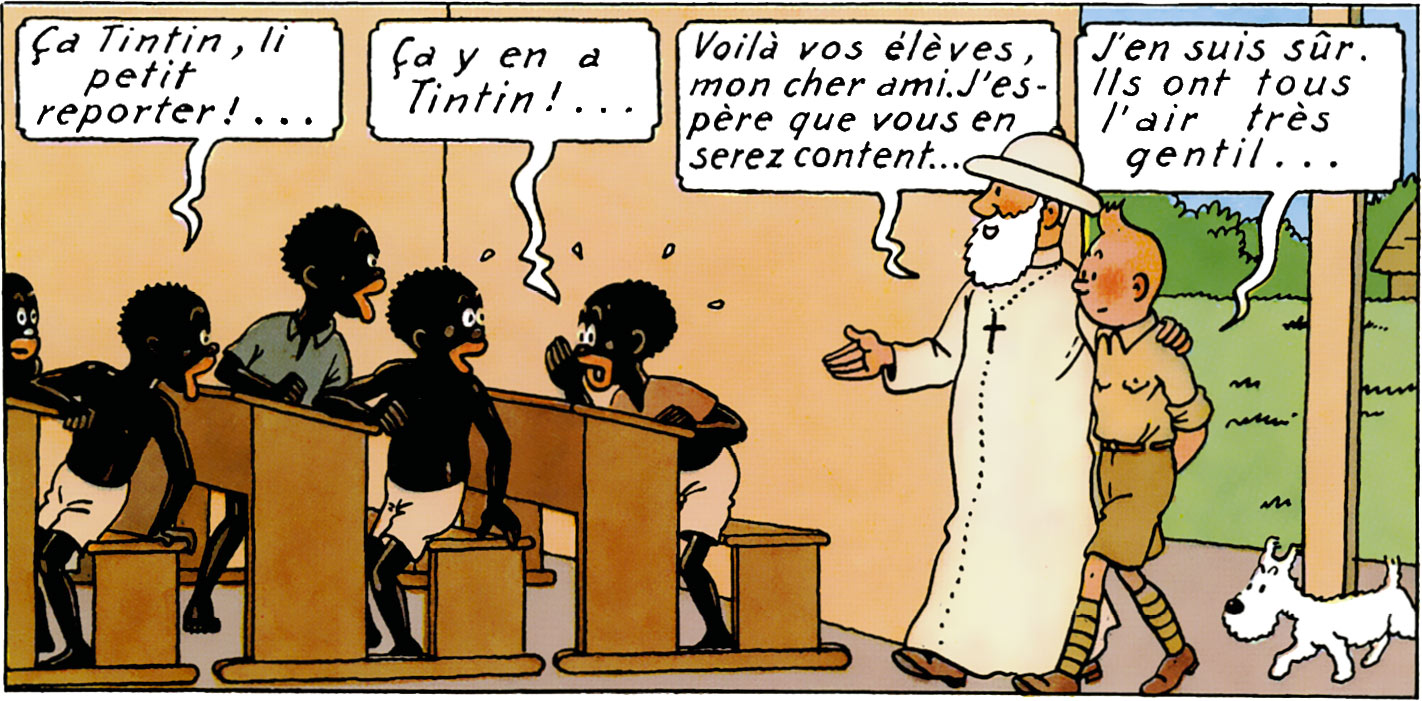
\includegraphics[width=\textwidth]{SeminaireMission/images/TintinCongo.jpg}

\paragraph{Un vocabulaire de conquête} "Position déjà acquise",.. le champ lexical est assez guerrier. 
Aujourd'hui, on n'emploie plus ces termes.



%--------------------------------------
\section{Rerum Ecclesiae}


\subsection{Présentation et biographie de l’auteur, Pie IX (1857-1939)}	

Pie XI, né Ambrogio Damiano Achille Ratti en Italie, est le Pape de l’entre-deux guerres (1922 à 1939). Si l’on jette un regard global sur son pontificat, très riche, c’est le Pape qui fait la transition entre chrétienté et monde moderne sécularisé. C’est certainement ce qui explique quelques paradoxes dans ses positions : 
\begin{itemize}
    \item  viscéralement anti communiste (il évoque dès sa 1ère encyclique, la lutte des classes comme « l’ulcère mortel des nations ») et il publie en mars 1937 \textit{Divini Redemtoris} qui condamne le communisme et le bolchevisme  ;  il sortira néanmoins une encyclique sociale\textit{ Quadragesimo anno} (QA) qui est la suite de \textit{Rerum novarum}, 40 ans après, dans laquelle il affirme le principe de subsidiarité. Dans ces 2 encycliques il confirme l’importance de mettre en place un syndicalisme chrétien et par ailleurs, il encourage la naissance de l’Action Catholique, notamment la JOC.                 \item La fête du Christ Roi, pour rappeler que le Règne de Dieu n'est pas à chercher dans un parti politique chrétien.
    
  \item  Dans 4 textes qui eurent un grand retentissement, il condamne le nationalisme exacerbé (Encyclique Ubi Arcano en 1922), l’action française (Allocution consistoriale en déc 1926), le fascisme (Encyclique Non abbiamo bisogno en 1931) et le nazisme (Encyclique \textit{Mit brenender sorge} mars 1937), et il sort ostensiblement de Rome quand Hitler vient dans la capitale italienne ; MAIS il s’entend néanmoins avec Mussolini avec qui il met fin à la querelle de Rome en signant en 1925 les accords du Latran. 
  \item  Sa vision de la religion est dit « intégraliste » c’est-à-dire que 
  
  \begin{quote}
      « son catholicisme intégral se conçoit comme une contre-culture alternative tant au libéralisme qu’au socialisme apportant ses propres réponses aux besoins de la société contemporaine, sans transiger avec la doctrine et les « erreurs [du] temps », autrement dit avec le modernisme. »
  \end{quote} Il freine par ailleurs des 4 fers l’ouverture de l’Eglise vers l’œcuménisme en ayant une vision unioniste, MAIS il prêche une égalité parfaite entre toutes les races, il évoque « l’universelle famille humaine » des peuples, qui « sont liés entre eux par des rapports de fraternité » (Ubi Arcano en 1922) et qui ont droit au respect, à la vie, à la prospérité, à la justice, et à la paix. Et devant le risque que représente la traque nazie des juifs, il n’hésite pas, selon la formule qui fera florès à se qualifier de « sémite ». 

  
\end{itemize}

Difficile donc de classer ce Pape, d’autant qu’au bout du compte, il restera surtout comme « le pape des missions » , comme nous allons le voir à présent.


\paragraph{Actions sur les missions}
\begin{itemize}
    \item Centralisation de l'oeuvre de mission de Pauline Jaricot à Rome (financement). Il cherchera à formaliser la machine financière.
    \item ordination des évèques chinois
    et japonais
    \item Ste Thérèse de l'Enfant Jésus, patronne des missions.
\end{itemize}



\subsection{Bibliographie consultée pour l’exposé}
 	

1.	Pie XI, Encyclique Rerum Ecclesiae sur les missions catholiques, 28 février 1926
2.	Benoit XV, Lettre apostolique Maximum illud, 1919
3.	BOUCHER André (Mgr)/ Institut Pie XI, L’action missionnaire, Paris, Librairie Bloud \& Gay, 1931, 226p
4.	PRUDHOMME Claude, « Chapitre 23 - La France et les missions catholiques, XVIIIe-XXe siècles » (p 375 à 390) in Alain Tallon \& Catherine Vincent (Sous dir), Histoire du christianisme en France, Collection U, Armand Colin, 2014, 448p 
5.	BRIA (Ion), Philippe CHANSON, Jacques GADILLE \& Marc SPINDLER, Dictionnaire œcuménique de missiologie – cent mots pour la mission ; Articles « 11 Clergé indigène (p50 à53) » par Paule Brasseur« 12 Colonisation (p53 à 56)» par J.Françis Zorn \& « « 69 Papauté et missions (p252 à 255) » par Claude Prudhomme, Paris CERF/Genève Labor et Fides/Yaoundé CLE, 2001, 394p
6.	DELACROIX (ss dir Mgr), Histoire universelle des Missions catholiques- T3 Les missions contemporaines (1800-1957) ; Chap 5 « l’avènement des jeunes églises Benoit XV, Pie XI et Pie XII » (p126 à 165), Paris, Librairie Grund, 1957, 447p
7.	COSTANTINI Cardinal, Réforme des Missions au XXème siècle, Paris, Casterman, 1960, 282p
8.	DESOUCHE Marie-Thérèse, « Pie XI, le Christ Roi et les totalitarismes » Dans Nouvelle revue théologique (Tome 130), 2008/4 , p 741 à 759
9.	ESSERTEL Yannick, Evangélisation et cultures – Essai d’histoire et d’anthropologie d’une pédagogie missionnaire du 1er au XXème siècle, CERF Patrimoines, 554p, 2021, Cote 297 411
10.	OOMS Toon, « Une ère nouvelle pour les missions - Le plaidoyer de Jean Bruls (1911-1982) pour un nouveau modèle missionnaire », dans Nouvelle revue théologique 2022/3 Tome 144, pages 452 à 470
11.	HILDESHEIMER Françoise, Une brève histoire de l'Église - Le cas français IVe-XXIe siècles ; chap9 « Modernistarum callidissimum artificium »,  Coll. Champs Histoire, Flammarion, 2019, 477p
12.	Ouvrage collectif, Théo – Nouvelle encyclopédie catholique, Droguet-Ardant/Fayard, 1989, 1236p
13.	Site du Vatican, notamment consultation des biographies des papes Benoit XV, Pie XI, Pie XII
14.	WIKIPEDIA, articles « Missions catholiques aux XIXe et XXe siècles » ; « Benoit XV » ; « Pie XI » ; « Pie XII » ; « encyclique Rerum Ecclesiae » « Lettre apostolique Maximum illud »


\subsection{Nature du texte et contexte historique et textuel}
 

L’Encyclique Rerum Ecclesiae est la 8ème encyclique de Pie XI, Pape particulièrement prolixe en encycliques  . C’est, nous l’avons dit, le « Pape des missions ». Il intervient dans une période particulièrement intense :  le personnel missionnaire passe de 1903 à 1925 de 15000 à 30000. Tout est doublé : les missions, les baptisés. Le Pape se sent donc appelé à organiser ces missions. Particulièrement actif dans les 8 premières années de son pontificat, il adopte une attitude presque militaire en centralisant dès la 1ère année de son pontificat, à Rome, en 1922, l'Œuvre de la Propagation de la Foi (créée par Pauline Jaricot à Lyon). En 1923, c’est la constitution des premières églises indigènes aux Indes et l’année d’après, le concile plénier de Shanghaï. Et en décembre 1924, il organise l’exposition missionnaire du Vatican temporaire (jusqu’au 10 janvier 1926) qui deviendra ensuite permanente, comme il le dit explicitement dans l’encyclique (création en novembre 1926 d’un musée ethnologique des missions au palais du Latran). Puis sort le 28 février 1926 l’encyclique Rerum Ecclesiae. Soucieux de l'ouverture du clergé aux indigènes, il sacre en 1926 les six premiers évêques chinois et l’année suivante le 1er Evêque japonais. Et fin 1927 il institue Ste Thérèse de Lisieux comme patronne des missions. Enfin en 1929, il réorganise et coordonne l’action de ses 3 grands instruments de la Mission, conformément à ce qu’il annonce dans l’encyclique Rerum Ecclesiae : les grandes œuvres pontificales de la propagation de la Foi (qui subvient aux besoins généraux de la Mission) ,  la Sainte Enfance (qui s’occupe des enfants des pays de mission) et St Pierre-apôtre (qui met en place et prend en charge les séminaires et la formation des prêtres indigènes). 

\subsection{L’encyclique}
\paragraph{L’objet et l’effet recherché}

C’est dans le contexte décrit précédemment que s’inscrit l’encyclique Rerum Ecclesiae. Elle porte le sous-titre suivant : « sur le développement à donner aux missions ». Elle s’adresse donc en premier chef aux responsables de Mission et de façon générale à tous les missionnaires. Mais cela va au-delà car Pie XI souhaite mobiliser tous les catholiques.
Il s’agit essentiellement premièrement de « booster » les missions en impliquant tout le peuple catholique ; il s’agit, deuxièmement, de réfléchir à la mise en place d’une part et à la formation, d’autre part, d’un clergé indigène à vaste échelle.


On ressent une certaine urgence dans cette encyclique : Pie XI se vit clairement comme un pape dont « le but [est] de répandre la lumière de l’Evangile et les bienfaits de la culture et de la civilisation chrétiennes aux peuples qui "étaient assis dans les ténèbres et dans l’ombre de la mort" », pour reprendre le tout début de son encyclique (§1).  


L’enjeu majeur, pour l’Eglise, en effet, c’est à la fois de développer, mais aussi de pérenniser ces avancées missionnaires sur des terres nouvellement christianisées. 
Le contexte missionnaire est le suivant : implicitement, en Afrique, en Asie,  les religions sont clairement en concurrence les unes les autres et il est clair que Pie XI ne souhaite se faire doubler ni par l’islam, ni par les protestants. L’heure n’est ni à l’œcuménisme (en tous cas, avec son approche unioniste, le Pape est très réticent vis-à-vis des prises d’initiatives qui se font jour) ni au dialogue interreligieux. Mais explicitement, c’est contre le paganisme qu’il se bat : il déplore le fait que les païens soient quasi 1 milliard (§4)

\paragraph{L’argumentation }
 

Souvent, l’Eglise est assimilée au colonisateur. Il y a donc un grand risque que celle-ci soit considérée comme une occupation étrangère par des missionnaires occidentaux. D’où l’urgence ressentie par le Pape de développer et former un clergé insulaire. Pie XI, pour le dire, reprend l’image de la vigne : « Pourquoi le clergé indigène serait-il empêché de cultiver son champ ? ». 

De plus, il se joue aussi un enjeu qui a à voir avec une certaine vision humaniste. De même que Lavigerie a été à la pointe du combat contre l’Esclavage, il est nécessaire de se battre aussi pour parvenir à une totale égalité entre le clergé européen et le clergé insulaire. C’est ce qu’évoque le Pape en parlant de stricte égalité dans la « dignité sacerdotale ».  Mais est-ce vraiment l’argument humaniste qui l'emporte ? N'est-ce pas plutôt une forme de réalisme au nom de l’efficacité missionnaire ? 
Car Pie XI reprend dans son encyclique un argument de Benoit XV figurant dans Maximum Eliud : 

\begin{quote}
    « le prêtre, par sa naissance, son tempérament, ses sentiments et ses intérêts est en contact étroit avec son propre peuple, il est au-delà de toute controverse à quel point il peut être précieux pour inculquer la Foi dans l’esprit de son peuple. Le prêtre autochtone comprend mieux que n’importe quel étranger comment procéder avec son propre peuple. » (§21). 
\end{quote}
Il rajoute un argument supplémentaire qui va dans le même sens : la connaissance imparfaite de la langue.

Par ailleurs, est pointé aussi le fait que l’Europe a elle aussi besoin de ses prêtres (23§). Il est d’ailleurs intéressant de noter cet argument à la lumière du 3ème texte étudié aujourd’hui de Pie XII : \textit{Fidei Donum} qui donnera à l’inverse la possibilité aux prêtres diocésains à répondre aux appels des missions d'outremer, notamment en Afrique et Amérique latine, tout en restant attachés à leur diocèse d'origine.

Le gros du développement du texte (à partir du §19), et le plus important, est consacré à la formation et au statut de ce clergé indigène. Il est affirmé -ce qui ne va pas de soi au moment où sort l’encyclique-  l’égalité dans la formation initiale, l’égalité dans les responsabilités, dans les missions données aux uns et aux autres. Et surtout, il est clairement préconisé l’ouverture de séminaires sur place. Il faut instruire les séminaristes indigènes de toutes les sciences modernes (sciences sacrées et profanes » est-il précisé §21). 

Pie XI évoque aussi l’opportunité de la création « de congrégations entièrement nouvelles, qui correspondraient mieux au génie et au caractère des indigènes et qui seraient plus en accord avec les besoins et l’esprit des différents pays. » Cela ne l’empêche pas de donner la Possibilité pour les indigènes de rallier des congrégations anciennes y compris des contemplatifs. 

Enfin il souhaite optimiser l’organisation de la mission, et implanter le christianisme en créant sur place des écoles, des hôpitaux, etc… 

 \paragraph{La valeur théologique du texte : une christologie de conquête et une ecclésiologie missionnaire qui s’inscrit dans la durée}


Le vocabulaire est un vocabulaire de conquête, somme toute pas très loin de l’expansionnisme colonial. Il s’agit de « gagner au Christ tous ceux qui ne le connaissent pas ou sont encore sans troupeau. »  Dans cette vision, le Pape se considère comme le « vicaire du Christ » (cela a été dit par Pie XI dans des discours)
Notons au passage au §5 un passage qui éclaire la vision intégraliste du Pape et qui témoigne d’une christologie très particulière : il importe pour lui en effet : « que nous essayions de mettre sous la domination du doux Christ autant d’autres hommes que possible ». Le Pape et partant l’Eglise en mission, s’apparentent à une armée. La christologie de Pie XI est fondée sur une vision hiérarchique au sommet de laquelle il y a le Christ. Et juste en dessous le Pape.  On rappelle que c’est Pie XI qui a instauré en 1925 la célébration du Christ-Roi qui met en avant la puissance du Jésus-homme …Toutefois il ne s’agit pas de prendre les armes mais de convertir. Et pour cela est mise en avant « l’autorité particulière du Pape sur les missions. » . Pie XI se situe clairement toujours dans une logique de chrétienté, mais ce sont bien les derniers soubresauts qui tomberont après la 2 GM.


Par ailleurs, concernant l’Eglise, ce qui est fondamentalement en jeu, c’est un changement de paradigme ecclésiologique et missionnaire : il s’agit d’avoir une vision de la Mission qui soit une approche temporaire, un état transitoire et passager. Il n’est plus question que s’implantent durant des siècles, comme cela avait pu se passer auparavant, des missionnaires étrangers qui s’inculturent. On n’en est plus là. Les missionnaires ont vocation à tout mettre en œuvre pour que se développe et se mette en place un clergé indigène, autochtone qui pourra, si on peut dire, passer la 2ème couche de l’évangélisation.
\paragraph{"Apporter la civilisation Chrétienne"} Vocabulaire qu'on n'utiliserait pas aujourd'hui mais qui inclut aussi les oeuvres - éducation, medecine .   

\begin{quote}
   
 p. 2 : idée de culture chrétienne.

« la dette de charité qui nous lie à Dieu exige non seulement que nous nous efforcions d'augmenter le nombre de ceux qui le connaissent et l'adorent " en esprit et en vérité " [3], mais encore que nous soumettions le plus grand nombre d'entre nous au règne du très aimable Rédempteur, afin que " l'utilité de son sang " [4] soit chaque jour plus féconde, et que nous lui soyons de plus en plus agréables, tandis qu'il lui plaît par-dessus tout que les hommes soient sauvés et parviennent à la reconnaissance de la vérité [5]. »

\end{quote}
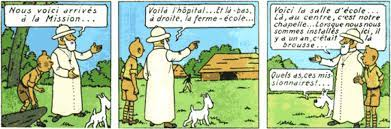
\includegraphics[width=\textwidth]{SeminaireMission/images/TintinCongo2.jpg}

\paragraph{Changement de vision sur la culture} Musée missionnaire avec les arts locaux
\paragraph{Continuité d'un certain vocabulaire de Maximum Illud}
\begin{quote}
    p. 10 
« « Il est bien vrai que la parole de Dieu et ses prédicateurs sont plus facilement reçus par les plus humbles roturiers ; il est vrai aussi que Jésus a dit de lui-même : " L'Esprit du Seigneur... m'a envoyé évangéliser les pauvres "[19] ; mais outre le fait qu'il faut se rappeler la parole de saint Paul : " Je suis redevable aux sages et aux insensés "[20], la pratique et l'expérience nous enseignent qu'une fois que les chefs du peuple ont été conduits à la religion du Christ, les classes les plus humbles suivent facilement. »
\end{quote}


Faut-il l’option préférentiel pour les pauvres ou alors toucher l’ élite ?
\begin{quote}
    
\end{quote}
« Les territoires confiés par le Saint-Siège à vos soins assidus, afin que vous les placiez sous la loi du Christ, sont pour la plupart d'une grande étendue. »

Logique territorial , RdD : sous la Loi du Christ.


\subsection{ Appréciation et discussion critique}
 

Il s’agit d’une encyclique qui amplifie, précise et applique la lettre apostolique du prédécesseur de Pie XI, Benoît XV Maximum Illud (du 30 novembre 1919 ) considérée comme « la grande charte des missions modernes ». Il y a donc beaucoup d’idées qui se trouvaient déjà en germe dans ce premier document comme la formation d’un clergé insulaire. Mais qui sont précisées. 


\paragraph{En chiffre}
Si l’on fait un bilan de la situation dans les années 30, soit 5 ans après cette encyclique, selon le livre L’action missionnaire, on parvient aux chiffres suivants : 3734 prêtres indigènes et 8279 prêtres étrangers soit 31\% d’autochtones. On voit donc que la politique que veut faire triompher Pie XI ne se concrétise pas massivement dans les faits. Elle sera stoppée par l’ouragan de la seconde guerre mondiale puis de la décolonisation.

Et si l’on prend, pour finir, un regard contemporain, force est de constater que dans tous les pays du monde à présent, se sont mis en place des clergés et des séminaires autochtones. On peut donc dire que de ce point de vue la vision de Pie XI a, de ce point de vue, triomphé.  Un triomphe tel que, par une totale ironie de l’histoire, c’est à présent ce "clergé indigène" -pour conserver un titre qui a extrêmement mal vieilli- qui vient aujourd’hui au secours des paroisses françaises ; et qui, sans lui, faute de vocation sacerdotale dans notre pays, ne seraient plus en mesure de fonctionner…               
 

\paragraph{Question sur la motivation du clergé autochtone} Est ce pour l'efficacité de la mission ou par vision égalitariste ?


\section{Fidei Donum}
Ce sont les deux mots latins en tête de l'encyclique du Pape Pie XII du 21 avril 1957. Fidei Donum. don de la foi. Ce sont les deux mots latins en tête de l’encyclique du Pape Pie XII du 21 avril 1957 intitulée « Fidei Donum » invitant les évêques à porter avec lui « le souci de la mission universelle de l’Eglise », non seulement par la prière et l’entraide, mais aussi en mettant certains de leurs prêtres et fidèles à la disposition de diocèses d’autres continents. Les prêtres envoyés, restent attachés à leur diocèse d’origine et y reviennent après plusieurs années passées en mission. On les appelle souvent « Prêtres Fidei donum.»

\paragraph{Un vocabulaire daté}
\begin{quote}
    Any delay or hesitation is full of danger. For the people of Africa have made as much progress toward civilization during the past few decades as required many centuries among the nations of Western Europe. Thus they are more easily unsettled and confused by the introduction of theoretical and applied scientific methods, \textbf{with the result that they tend to be unduly inclined to a materialistic outlook on life}. Hence a condition of affairs is sometimes brought about that is difficult to correct and in the course of time may prove to be a great obstacle to the growth of faith, whether in individuals or in society at large. For this reason it is imperative that help should be given now to the shepherds of the Lord's flock in order that their apostolic labors may correspond to the ever-growing needs of the times.
\end{quote}


 \begin{quote}
     57. Nous pourrions nous demander, en outre, si nos prières viennent d'un cœur sincère si nous prions pour le succès des missions sans accompagner nos prières d'offrandes charitables selon nos moyens. Nous connaissons bien - en fait, mieux que quiconque - la libéralité abondante de Nos fils, comme en témoignent constamment de nombreux exemples merveilleux. A ces âmes généreuses est due, sans aucun doute, le merveilleux essor de nos missions depuis le début de ce siècle. En conséquence, nous désirons exprimer notre profonde gratitude à nos fils et filles bien-aimés qui contribuent par leurs efforts zélés et leur soutien caritatif à de nombreuses entreprises missionnaires.
 \end{quote}

 \begin{quote}
63. L'Église en Afrique, ainsi que dans d'autres parties du champ missionnaire, a besoin de missionnaires. C'est pourquoi Nous vous appelons une fois de plus, Vénérables Frères, en vous priant de faire preuve de zèle avec toutes les ressources dont vous disposez pour soutenir tous ceux qui ont été divinement appelés à assumer les charges de l'apostolat missionnaire, qu'ils soient prêtres ou religieux et femmes.
     
 \end{quote}

 \paragraph{Etudiants africains}
 \begin{quote}
     71. Avec le même intérêt affectueux qui joint ses efforts à ceux des autres dans une harmonie fraternelle et exclut toute considération égoïste, veillez particulièrement à accorder un soin spirituel aux jeunes d'Afrique et d'Asie, qui résident peut-être dans vos diocèses en vue de leur poursuivre leurs études.

72. Ces jeunes hommes, déracinés par les bouleversements sociaux dans leur propre pays, n'ont souvent pas, pour de nombreuses raisons, suffisamment de contacts sociaux catholiques parmi les personnes qui les accueillent. De ce fait, leur vie chrétienne peut être mise en danger, car les vraies valeurs et excellences de la nouvelle culture qu'ils recherchent peuvent leur échapper et ils peuvent, en conséquence, être séduits par les doctrines du matérialisme et succomber aux flatteries des coteries athées. Vous ne pouvez pas ignorer l'impact de cela sur leur carrière actuelle et future. Ce serait une bonne idée de nommer des membres du clergé dévots et bien équipés pour prendre en charge cet apostolat, soulageant ainsi les inquiétudes de leurs propres évêques dans les champs de mission.
 \end{quote}

 \paragraph{Regard égalitariste entre les jeunes églises} 

 \paragraph{Solidarité entre Eglises} Don à court terme d'un prêtre et non jusqu'à la mort. Temps limité du prêtre au service de l'Eglise. 

\paragraph{Civilisation chrétienne}


un contexte marxiste anti-religieux.


  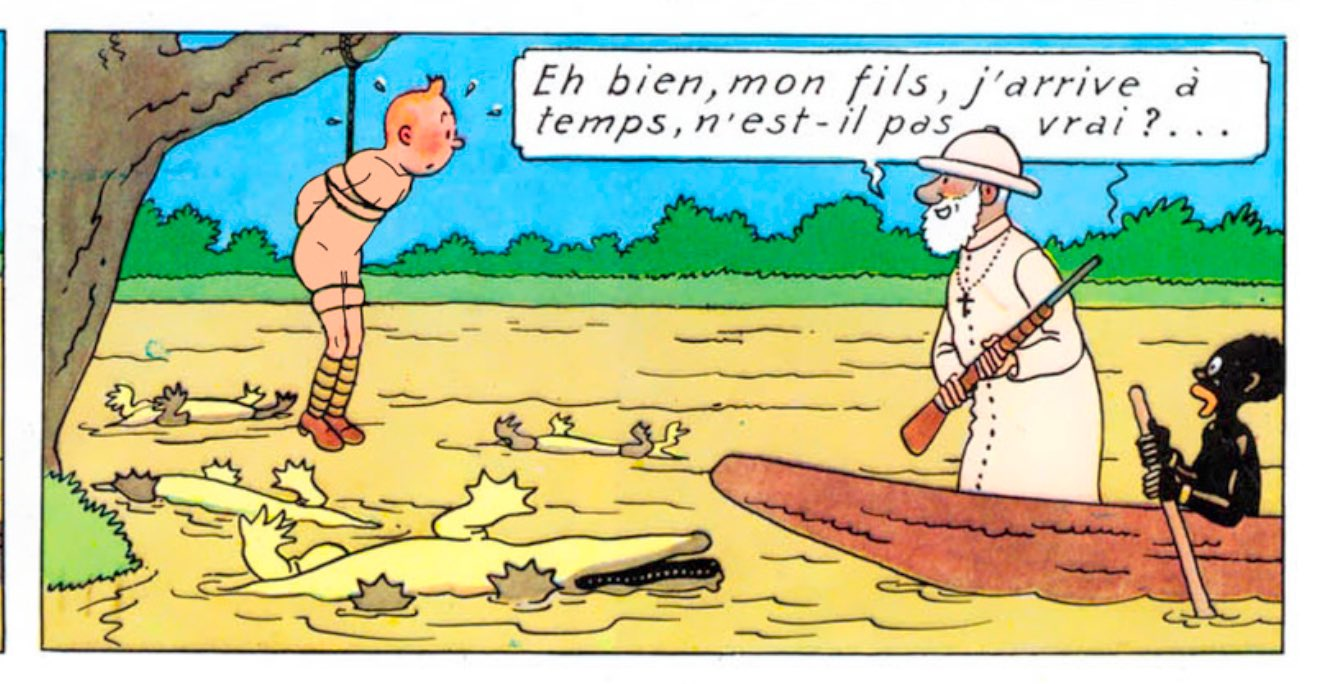
\includegraphics[width=\textwidth]{SeminaireMission/images/TintinCongo3.jpg}  


 
\section{Bilan}

\paragraph{sur la forme} du séminaire
Démarche chronologique pertinente. Continuité et modification.
distance avec ces textes, y compris de Vatican II.

\paragraph{sur le fond} prendre deux ou trois points que nous retenons de ce séminaire.

Mission : dialogue, nous force à creuser notre foi.

Occasions manquées, en particulier avec FX et Matteo Ricci.

Marie de l'Incarnation, bonne surprise et le plan pour le Quebec.

Question ouverte : sur la figure du prophète, qui détruit les idoles, et la figure sapientielle de l'ouverture aux autres. FX : actualité, dans Laudato Si.  





\chapter{Ad Gentes - Concile Vatican II}


\section{Préparation}
\paragraph{Plan}
Préambule (1)

Principes doctrinaux (2-9)

L’œuvre missionnaire elle-même (10-18)
\begin{itemize}
    \item Introduction (10)
  \item Le témoignage chrétien (11-12)
  \item La prédication de l’Évangile et le rassemblement du Peuple de Dieu (13-14)
  \item La formation de la communauté chrétienne (15-18)
\end{itemize}
 
Les Églises particulières (19-22)

Les missionnaires (23-27)

L’organisation de l’activité missionnaire (28-34)

La coopération (35-41)

Conclusion (42)

\subsection{Lecture attentive}
\begin{itemize}
    \item \paragraph{Principe doctrinaux} : 
    \begin{itemize}
        \item  Dieu veut nous rassembler en un peuple\mn{Jn 11, 52 Et ce n'était pas pour la nation seulement; c'était aussi afin de réunir en un seul corps les enfants de Dieu dispersés.}
        \item la mission du fils : Dieu s'engage dans l'histoire humaine.
        \item Mission du saint esprit : \textit{pousse l'Eglise à s'étendre. }
        \item l'Eglise envoyée par le Christ.  \textit{C'est de là (Allez baptiser...) que découle pour l'Eglise le devoir de propager la foi et le salut apportés par le Christ. } 
        \item l'activié missionnaire : Évêques.  \textit{la mission est unique et la même partout, en toute situation, bien qu'elle ne soit pas menée de la même manière du fait des circonstances}
    \end{itemize}
   \item les Eglises particulières
    
\end{itemize}

\paragraph{Rôle des évêques} Après des textes sur l'activité missionnaire centralisée, rôle des évêques. Car la mission ne se pense plus comme les \textit{missions} (quand il n'y a pas d'Eglise en un lieu)

\paragraph{Insistance à l'universalité} \textit{la mission est unique et la même partout, en toute situation, bien qu'elle ne soit pas menée de la même manière du fait des circonstances} -6)

\begin{quote} AG 16
    Ces exigences communes de la formation sacerdotale, même pastorale et pratique, selon les dispositions du Concile [47], doivent se combiner avec le zèle à prendre en considération le mode particulier de penser et d’agir de son propre peuple. Les esprits des élèves doivent donc être ouverts et rendus pénétrants pour bien connaître et pouvoir juger la culture de leur pays ; dans les disciplines philosophiques et théologiques, ils doivent saisir les raisons qui créent un désaccord entre les traditions et la religion nationales, et la religion chrétienne [48]. De même, la formation sacerdotale doit tenir compte des nécessités pastorales de la région ; les élèves doivent apprendre l’histoire, le but et la méthode de l’action missionnaire de l’Église, et les conditions particulières d’ordre social, économique, culturel de leur propre peuple. Ils doivent être éduqués dans un esprit d’œcuménisme et préparés comme il convient au dialogue fraternel avec les non-chrétiens [49]. 
\end{quote}


\paragraph{Transformation} Il n'est pas rare que les groupes humains au sein desquels l'Eglise existe, ne soient complètement transformées pour des raisons diverses. des situations nouvelles peuvent en résultaer (6)

\paragraph{Divisions des chrétiens} 6

\begin{Synthesis}
    L’activité missionnaire n’est rien d’autre et rien de moins que la manifestation du dessein de Dieu, son épiphanie et sa réalisation dans le monde et son histoire, dans laquelle Dieu conduit clairement à son terme, par la mission, l’histoire du salut. 9
\end{Synthesis}

% \chapter{Lire les classiques Chinois}

 

\textbf{Comment lire les classiques chinois ? (French Edition)}

\textbf{Vermander, Benoît}

\section{Prologue}


\subsection{Période axiale}
  \mn{ p. 5 · E. 59  } \begin{quote}
Lorsque la notion même de « période axiale » est acceptée au moins comme
hypothèse de travail ( elle est parfois rejetée dès l'abord ) , les
percées qu'on lui associe sont généralement les suivantes : ( a ) les
penseurs de la période auraient contribué à « problématiser le monde »
plutôt qu'à le recevoir tel quel , ce par le fait d'articuler la réalité
sociale autant que naturelle autour de questions portant sur son «
pourquoi » et son « comment » ; ( b ) c'est ainsi qu'aurait émergé la «
conscience critique » , l'examen des opinions reçues , la remise en
cause d'au moins certaines des structures sociales ; ( c ) ce
questionnement
aurait nourri un souci éthique ( à moins que ce dernier ait contribué à
l'émergence de la conscience critique ) , souci qui fut accompagné
souvent de la formation d'une vision utopique -- la cité idéale de
Platon , la pleine libération des individus dans le bouddhisme , le rêve
d'un ordre social gouverné par les rites , l'éducation morale , chez
Confucius , l'annonce de la venue du Royaume de Dieu chez les prophètes
d'Israël ; ( d ) le surgissement critico - éthique aurait été porté par
des personnalités incarnant les « sauts » entrepris , personnalités dont
le nom est transmis aux générations qui leur succèdent ; ( e ) ces
personnalités sont souvent représentées ( et semblent s'être considérées
elles - mêmes ) comme des « Renonçants » , des individus dont les choix
de vie mettent en question l'ordre dominant : dans la République , le
philosophe de la cité idéale de Platon renonce aux possessions privées
et à la vie de famille pour gouverner la Cité avec justice

\end{quote}  

\subsection{Divination, mathématique et concepts}
\mn{- p. 17 · E. 258  } \begin{quote}  

Élaborer des ramifications entre les principaux viscères du corps humain
et les états climatiques ( le chaud , le froid , le sec , l'humide ) ,
les émotions , les notes de musique , les couleurs , tout cela transcrit
dans une arithmétique de
base cinq » , n'est pas simple opération de l'esprit mais permet bien
d'observer pragmatiquement un ensemble de correspondances . En même temps, ces analogies deviennent moralement signifiantes. C’est ainsi que s’opère une évolution du divinatoire au combinatoire et à l’éthico-politique.   
A la fois matrice de ce processus et l'accompagnant tout au long de sa
formation textuelle , le \textit{Classique des mutations ( Yijing )} construit un
métalangage de l'univers à partir d'une réflexion mathématisée sur les
processus de divination.
il s'essaie à décrire la façon dont les phénomènes se suivent et
s'agencent de façon nécessaire . C'est , à l'extrême , une mathématique
de tous les phénomènes possibles , fondée sur l'idée que tout n'existe
que dans l'échange , le passage , la fluidité : la gradation est un
autre nom du contraste , et la logique des transformations ( des
changements par quoi une forme entre en contraste avec celles qui la
précèdent et la suivent ) , non pas celle des oppositions , régit
l'univers et la pensée .

\end{quote} \mn{ p. 18 · E. 268 } \begin{quote}

Au ciel se composent les images {[} xiang {象} {]} , sur la terre se
composent les formes {[} xing 形 {]} , et les transformations se font
visibles {[} Yijing , Xici 繫辭 I . 1 {]} 28 .

\end{quote} 

\paragraph{le rite comme éducation} chez Confucius
\mn{p. 20 · E. 304  } \begin{quote}

Le vecteur de l'éducation ainsi dispensée , ce sera le rite
: l'éducation de l'intérieur par l'extérieur . À noter pourtant que « le
rite » ( chinois ) et « la loi » ( en contexte grec ou hébreu ) ne se
trouvent pas dans un strict régime d'opposition : ils régulent tous deux
les conduites extérieures jusqu'au moment où les prescriptions se
retrouvent être inscrites « au fond des cœurs » .

\end{quote} \mn{ p. 24 · E. 367 } \begin{quote}

La détermination d'un corpus de classiques fonde une culture dans sa
spécificité tout en lui donnant d'affirmer son l'universalité latente .
Hans - Georg Gadamer fait de l'extensibilité ,  en principe illimitée, de la durée pendant laquelle une œuvre communique son sens le trait qui désigne un « classique »
\end{quote} 
 
\section{Chapitre I : Qu'est-ce qu'un classique chinois ?}

\mn{ p. 37 · E. 786 } \begin{quote}

Du reste , dès les premiers rencontres entre lettrés chinois et
missionnaires occidentaux , les uns et les autres comprennent que le
continent qui leur fait face est fondé sur une armature de classiques
dont la maîtrise est essentielle pour la réussite culturelle ,
religieuse et sociale , et ils feront de la connaissance réciproque de
ces textes la clé d'une rencontre possible , d'une entrée dans la pensée
de l'Autre , que ce soit pour l'apprécier ou l'utiliser , pour
convaincre ou dominer l'interlocuteur .

\end{quote} \mn{p. 38 · E. 805  } \begin{quote}
On trouve cette acception chez Yang Xiong 揚雄 (53 AEC-18) :

 
 \begin{quote}
     : « Un texte qui ne se mesure pas aux Classiques n’est pas un texte. Une parole qui ne se mesure pas aux Classiques n’est pas une parole. Ce sont des excroissances qui prolifèrent  
 \end{quote}
La formule, très concise, pourrait aussi être comprise comme signifiant : « Un texte qui n’est pas (qui ne tend pas au) Classique n’est pas un texte. » Ou même plutôt : \textit{« Un texte non référé à une norme n’en est pas un. »} Le registre sémantique du passage 11 rappelle celui qui entoure le terme déjà évoqué κανών : l’instrument qui norme (la règle du charpentier en grec) donne naissance à un ensemble textuel établi par rapport à lui – ensemble qui, de normé, devient alors normatif.
 
\end{quote} \mn{p. 44 · E. 926  } \begin{quote}

Pouvoir {[} di {]} d'en haut {[} shang {]} » surplombe le monde
surnaturel ( ne parlons pas d'un « panthéon » ,car on n’y trouve pas l’individuation des divinités qu’on attache d’ordinaire à ce terme).

 

\end{quote} \mn{ p. 45 · E. 951 } \begin{quote}

L'autre chapitre des Documents sur lequel nous nous arrêterons
brièvement est celui du Hongfan 洪 範 , expression que l'on peut
traduire par « Grand plan » ou , sans doute plus justement , par «
Modèle universel » . Il présente l'ensemble des phénomènes ( éléments ,
conduites , matières politiques , calendrier , sources de bonheur et
malheur ) sur des combinaisons fondées sur les chiffres Cinq et Neuf .
Sa composition apparaît si rigoureuse que certains formalistes russes
ont spéculé sur son nombre de caractères et leur inscription à
l'intérieur d'un carré magique 30

\end{quote} 

\paragraph{les annales historiques} attribuées à Confucius : essayer de dicerner les signes des temps. 
\mn{ p. 56 · E. 1164 } \begin{quote}
les lecteurs de ces Annales vont s’employer à faire émerger des sens, à trouver l’expression du mandat du Ciel dans cette succession d’événements qu’ils vont lire comme une sorte de rébus. C’est dire que ce sont les commentaires suscités par l’œuvre qui en font tout l’intérêt.
[..]
Au travers de la sèche prose des Printemps et
  Automnes , le Gongyang s'emploie à trouver « le sens profond de paroles
subtiles"
\end{quote}


Importance du processus de mémoire.

 \mn{p. 59 · E. 1228  } \begin{quote}

Au travers de cet hommage rendu par les historiographes du Zuozhuan à
leurs prédécesseurs se donne à lire leur conviction : l'enregistrement
et la qualification fidèles des événements sont questions de vie ou de
mort . Cela parce que l'enchaînement des actions , des prédictions que
l'on en tire , de la vérification ou non de ces prédictions constitue la
trame de l'ordre du monde , et qu'en altérer le récit , c'est forcément
en distordre la marche .

\end{quote}

\paragraph{Anectdote : matériau de la connaissance historique} car elle offre un aperçu soudain sur une réalité plus profonde et étendue, comme la citation. \mn{ p. 59 · E. 1233 } \begin{quote}
Du fait de la nature même de ces deux extraits, on aura noté la place que joue, dans le Zuochuan, le genre littéraire très particulier de l’anecdote.
 
Elle est révélatrice d'une tendance plus générale : l'anecdote , dans
l'historiographie chinoise , deviendra le matériau même de la connaissance historique.
 

\end{quote} 
\subsection{le sacrifice comme lieu de l'unité}
Une partie des textes classiques visent à expliquer la tenue en cas de non respect du sacrifice. Cette importance peut étonner.
\mn{p. 65 · E. 1345  } \begin{quote}

C'est en distinguant qu'on peut droitement unir .
Le

mode de découpe de l'animal sacrifié puis la façon dont on répartit les
parties découpées constituent des opérations destinées à symboliser et
réaliser la cohésion du groupe , dans un modèle qui associe exigence
d'unanimité et affirmation de principes hiérarchiques stricts . 

\end{quote} \mn{ p. 66 · E. 1353 } \begin{quote}
Le sacrifice
était donc image inversée de l'ordre social effectif . La supériorité
sociale était étroitement associée à la capacité de donner .

\end{quote} \mn{  p. 66 · E. 1356 } \begin{quote}

Les anomalies rituelles relevées par les textes fonctionnent alors comme
informations historiques d'importance particulière . La crise rituelle
est toujours symptôme de crise politique .

\end{quote} \mn{ p. 66 · E. 1357 } \begin{quote}

le Liji traduit une anxiété face à tous les dysfonctionnements possibles
de l'activité rituelle , et , de ce fait , du travail social .

\end{quote} \mn{p. 67 · E. 1368  } \begin{quote}

Le rituel est donc affecté par une tension entre son but avoué -- édifier ,
maintenir un ordre -- et le fait qu'il soit par essence une entreprise
risquée , soumise à divers aléas .

\end{quote} 
\subsection{La grande Etude - Daxue}
\mn{p. 67 · E. 1384  } \begin{quote}

Tentons après tant d'autres une traduction de cette célébrissime entrée
en matière -- sachant qu'aucun lecteur ni commentateur n'arrive à faire
vraiment abstraction de la lecture qu'en ont effectué Zhu Xi et ses
continuateurs . 
\begin{quote}
    La voie de la Grande Étude 96 , c'est d'éclairer {[} le
principe de {]} vertu qui {[} lui - même {]} éclaire {[} toute chose {]}
, c'est d'aimer {[} ou bien de « renouveler » , selon les versions {]}
le peuple , et c'est de ne s'arrêter qu'une fois la plus haute
perfection atteinte . Sachant le terme , on prend sa détermination . Une
fois déterminé , on peut s'apaiser {[} jing 靜 97 {]} . Une fois apaisé
, on peut s'ancrer dans la paix . Quand on est ancré dans la paix , on
peut discerner . Ayant discerné , on peut atteindre le but . Les plantes
ont racine et branches , les affaires un commencement et une fin . Celui
qui sait la succession des affaires , il est tout proche de la voie .
大學之道,在明明德,在親[新]民,在止於至善。知止而后有定,定而后能靜,靜而后能安,安而后能慮,慮而后能得。物有本末,事有終始,知所先後,則近道矣。


\end{quote}


\end{quote} \mn{ p. 69 · E. 1411 } \begin{quote}

La partie gauche du caractère , sa clé sémantique , c'est le jade ( yu 玉 )
. Associée à l'autre partie du caractère , cette clé donne à l'ensemble
un tour plus abstrait : elle parle d'une structure sous - jacente aux
phénomènes qui prennent corps . Les Chinois ont trouvé dans les nervures
du jade la plus marquante des expressions des forces vitales qui , à
l'interne , structurent l'organisme.

\end{quote} 
\paragraph{L'invariable milieu, à l'autre extremité des quatre livres}
\mn{ p. 69 · E. 1420 } \begin{quote}
Comme pour la Grande Étude, voyons à traduire le premier paragraphe du texte :
\begin{quote}
La loi du Ciel 101, c’est ce qu’on appelle « la nature » 102. Se conformer à la nature, c’est ce qu’on appelle « la voie ».
\ldots

   Aussi , l'homme de bien se tient sur ses gardes même quand il ne
distingue rien {[} d'inquiétant {]} , il craint et tremble même quand
rien ne frappe son oreille . 
 
\ldots

Aussi , l'homme de bien reste sur ses gardes {[} même {]} dans la
solitude 104 . N'émettre {[} fa 發 {]} ni joie ni colère ni tristesse ni
allégresse , c'est ce qu'on peut appeler l'équilibre {[} le milieu {]} .

\end{quote} 
\end{quote}

Relecture

\paragraph{Xunzi : la discrimination fait l’homme
 }
\mn{ p. 72 · E. 1482 } \begin{quote}

On a argué , à mon sens fort justement , que le caractère fen 分 (
séparer , diviser ) constitue une clé -- sinon la notion clé -- du Xunzi
112 . Le fait que l'on compte 113 occurrences du caractère dans
l'ouvrage est un premier signe de son importance .

\end{quote} \mn{ p. 73 · E. 1493 } \begin{quote}

le principe de base sur lequel Xunzi fonde sa théorie politique est que
les désirs ( par essence subjectifs ) sont par nature illimités , tandis
que les biens sont objectivement limités ( yu duo er wu gua 欲 多 而 物
寡 113 ) . Savoir comment répartir et partager , c'est bien là l'essence
de l'art politique 114 . Xunzi pose ici l'accent sur la notion de gong
公 : gong ( habituellement traduit par « chose publique ») consiste à diviser quelque chose avec impartialité, sans afficher égoïsme ou partialité (si 私).
 

\end{quote} \mn{ p. 74 · E. 1510 } \begin{quote}
Le rituel, manifestation privilégiée des distinctions ainsi effectuées, devient alors le conduit par quoi ce qui était au départ
de l'ordre de la nature ( xing 性 ) se transforme en artifice ( wei 偽 )
, ce dernier terme revêtant un sens éminemment positif
 
\end{quote} 
Sens positif de l'artifice chez xunxi.
\begin{Def}[artifice]

\end{Def}
\mn{ p. 74 · E. 1522 } \begin{quote}

Xunzi trace une distinction entre les niveaux atteints respectivement
par le Lettré ( shi 士 ) , l'homme de bien ( junzi 君子 ) et le sage (
shengren 聖人 ) , ce dernier seul capable de fusionner en un tout la
perfection des dispositions à l'interne et celle atteinte par les
observances extérieures .



\end{quote}


Cf vie digne et vie parfaite

\mn{p. 75 · E. 1527  } \begin{quote}

Les châtiments contribuent à assurer l'équilibre entre hiérarchie et
impartialité .

\end{quote} \mn{ p. 76 · E. 1550 } \begin{quote}

Xunzi voyait bien la nature humaine ( xing 性 ) comme mauvaise ( e 惡 )
, il discernait dans l'artifice rituel couplé à la droite éducation la
route par laquelle s'ouvrait la possibilité de dépasser l'inné , jusqu'à
rendre chacun capable de devenir -- en théorie -- semblable aux sages souverains du temps passé. Route trop dangereuse pour le Hanfeizi, quand les États font face à des risques imminents (la principauté dont Han Fei est un dignitaire éminent va disparaître trois ans après sa mort).
 
L'art politique ne consiste pas à éduquer le peuple , que ce soit par
les rites ou par la vertu , mais à instaurer un ordre durable au moyen
des châtiments et récompenses attachés à des lois valables pour tout un
chacun . Notons que
les Légalistes systématisent ici une vue politique apparue bien
auparavant , mais à laquelle les penseurs classiques avaient jusqu'alors
été à même de s'opposer : le Zuozhuan relate qu'en 536 AEC , l'État de
Zheng 鄭 fonde dans le bronze un code des châtiments . Il reçoit une
algarade d'un ministre de l'État de Jin 晉 , qui rappelle à tous que les
anciens rois comptaient , pour assurer l'ordre public , sur le rituel ,
le sens de la justice , l'attrait des positions officielles , l'exemple
donné par leur dévouement constant \ldots{} Ils savaient que l'existence
même d'un code intangible ne pouvait que corrompre la fibre morale d'un
peuple 116 . Pourtant , vingt - trois ans après cet épisode , l'État de
Jin cède à la même tentation 117 \ldots{} Nous approchons là de la fin
des récits du Zuozhuan :

\end{quote} \mn{p. 77 · E. 1580  } \begin{quote}
Ou encore comme le roi-sage taoiste,  \begin{quote}
    il
agit par le non agir ( wei wu wei 為 無為 ) 
\end{quote}, mais s'il est en mesure
de procéder ainsi c'est parce qu'il a institué l'artifice d'un corps de
loi simples , compréhensibles , adaptées au temps présent et cependant
universelles par leur inspiration , des lois qui , en quelque sorte ,
gouvernent à sa place -- pour autant qu'elles soient conformes à l'ordre
naturel : Les choses ont leur usage , les talents leur emploi . Lorsque
tout est en place , alors on n'a pas à s'activer du haut vers le bas .
Ordonnez à un coq de proclamer l'aube , ou à un rat de chasser les
souris ! {[} Hanfeizi , Yangquan , 1 {]} .

\end{quote} \mn{p. 79 · E. 1614  } \begin{quote}

Voyant un teinturier teignant la soie , Mozi dit tout en soupirant : Ce
qu'on teint en bleu devient bleu , ce qu'on teint en jaune devient jaune
. Quand on change {[} la teinture {]} dans quoi l'étoffe est immergée ,
change pareillement sa couleur . Trempée cinq fois , sa couleur
nécessairement changera cinq fois . Lorsque l'on teint , on ne saurait
être trop prudent {[} Mozi , Suoran , 1 {]} . 子 墨子 言 見 染 絲 者 而
歎 曰 : 「 染 於 蒼 則 蒼 , 染 於 黃 則 黃 。 所 入 者 變 , 其 色 亦
變 。 五 入 必 而已 , 則為 五色 矣 。 故 染 不可 不慎 也 。 」

\end{quote} \mn{p. 82 · E. 1666  } \begin{quote}

La partialité insère des négations dans une réalité de soi toute marquée
par l'affirmation . En contraste : l'attitude inclusive ( impartiale )
est toute positive :
\begin{quote}
    « Je fais pour l’autre comme pour moi-même » (wei bi wei you wei ji ye 為彼猶為己也, Mozi, Jian’ai, III, 2).
 
\end{quote}
\end{quote} \mn{p. 83 · E. 1695  } \begin{quote}

Pareille étincelle pourrait être par exemple la « découverte » faite par
Mozi que l'amour n'apporte bénéfice effectif que pour autant qu'il
s'abstienne de discriminer , de hiérarchiser . Il est plus aisé
d'imaginer que pareil basculement fut à l'origine de l'attraction
exercée par Mozi que d'y voir un développement « naturel » ( on ne voit
pas du reste en quoi il serait tel ) d'un appel initial à la simple
bienveillance .

\end{quote} 
\paragraph{des écrits pour se taire}
\mn{ p. 84 · E. 1701 } \begin{quote}

EN décalage peut - être plus grand encore que les textes mentionnés à
l'instant , dans la mesure où leurs principes épistémologiques diffèrent
profondément de ceux défendus par les lettrés ( shi 士 ) , le Daodejing
道德 經 ( ou Laozi 老子 ) et le Zhuangzi 莊子 comptent parmi les textes
les plus influents de la pensée chinoise -- et universelle .
\end{quote}
 
 \chapter{Méthodologie~: Pour lire et exposer un article}

\paragraph{Le plan des exposés}

\paragraph{11. Le temps de l'investigation}

\paragraph{111. Première lecture «~affective~» ou «~réactive~»}

Vous parcourez le texte, tentez de saisir d'où il part et où il va en
comparant l'introduction et la conclusion et en repérant les éléments
d'information donnés par les sous-titres, ce que vous aimez ou non à
première vue. Vous relevez votre premier intérêt et vos incompréhensions
ou désaccords, dans l'idée que, très généralement l'auteur a en fait
déjà répondu à vos objections.

Après cette première approche, vous pouvez vous engagez dans une étude
approfondie du texte.

\paragraph{112. Lecture pas à pas}

Vous commencez par numéroter les paragraphes page par page en adoptant
la convention suivante~: la première ligne en haut d'une page marque
toujours le commencement d'un paragraphe, même si elle commence au
milieu d'une phrase.

Vous lisez paragraphe par paragraphe et vous notez le contenu essentiel.
Ce travail que tous doivent faire pour préparer la séance n'est pas
nécessairement destiné à être restitué, mais est essentiel pour préparer
l'étape suivante.

\paragraph{113. Etablissement de la problématique de l'auteur}

Après la phase de lecture pas à pas, vous construisez la question à
laquelle l'auteur s'affronte~:

\begin{itemize}
\item
  pourquoi l'auteur se bat-il~?
\item
  quel problème essaie-t-il de régler, d'éclairer~? En général, il n'est
  pas difficile de trouver exposée la problématique en toute lettre dans
  le texte lui-même -- parfois même de manière redondante~;
\item
  en fonction de quel contexte culturel, social, culturel, économique,
  politique l'auteur construit-il sa problématique~? Notez les
  événements déterminants auxquels il se réfère et les auteurs qu'il
  évoque -- plus ou moins explicitement -- comme ses alliés ou ses
  adversaires -- et le cas échéant, renseignez-vous sur eux.
\end{itemize}

\paragraph{114. Etablissement de la thèse}

En fonction de la problématique de l'auteur, vous établissez la thèse de
l'article ou du texte étudié~: quelle solution l'auteur apporte-t-il à
sa question~? quelle perspective établit-il~? Là encore, il n'est pas
difficile de trouver cette thèse exposée de manière explicite dans le
texte lui-même.

\paragraph{115. Etablissement de l'argumentation}

Dans une seconde lecture, vous reconstruisez la logique argumentative en
fonction de laquelle l'auteur établit sa thèse.

\paragraph{116. Vérification}

Vous sélectionnez l'un ou l'autre extrait du texte (au maximum une page)
qui vous apparaît particulièrement décisif. Vous les ferez travailler à
l'ensemble du groupe, afin de vérifier dans les faits la justesse de
votre exposé.

\paragraph{117. Appréciation critique}

Enfin, vous concluez en, évaluant si l'auteur a atteint son but, dans
quelle mesure sa question était bien posée, sa thèse éclairante et
originale, sa démonstration convaincante. Et vous faites valoir l'apport
que votre exposé constitue pour la recherche du séminaire.

\paragraph{12. Le temps de l'exposition (20 mn)}

\paragraph{121. Biographie de l'auteur}

Efforcez-vous de présenter rapidement en quelques lignes l'auteur de
l'article étudié, et si possible, de situer plus brièvement les auteurs
avec lesquels il débat.

\paragraph{122. Bibliographie}

Notez l'ensemble des textes et références auxquels vous avez eu recours
pour préparer l'exposé, y compris vos sources pour la biographie et les
sites internet visités.

\paragraph{123. La problématique (cf. supra) (ce n'est pas un résumé).}

\paragraph{124. La thèse (cf. supra)}

\paragraph{125. L'argumentation (cf. supra)}

Vous pouvez vous appuyer sur vos notes de lecture pas à pas et sur le
texte sélectionné pour la vérification.

\paragraph{123. Appréciation et discussion critique}

\paragraph{2. Les comptes-rendus (ou synthèses)}

Les comptes-rendus permettent de garder une mémoire des avancées de la
recherche commune.

L'étudiant chargé du compte-rendu de la séance veillera à relever de
manière synthétique~:

\begin{itemize}
\item
  les acquis recueillis lors de la séance de travail~: rappel de la
  problématique, de la thèse, principales conclusions~; principaux
  éléments du débat~; critiques adressées à l'auteur~;
\item
  les acquis pour la suite du séminaire~: nouvelle manière de
  questionner, réponses obtenues à des questions antérieurement
  soulevées, découvertes d'horizons nouveaux etc.
\end{itemize}

Le compte-rendu prendra la forme d'une note de deux pages maximum qui
sera distribué à l'ensemble des participants au séminaire et rapidement
discuté en début de la séance suivante.


\section{Présenter un texte lors d’un séminaire}


\begin{Prop}
Attention !
-	La présentation ne doit pas dépasser 20 mn
-	Il ne s’agit pas de faire le résumé d’un texte que tous les participants ont déjà lu
\end{Prop}


\paragraph{1.	Présentation et biographie de l’auteur 
}
Efforcez-vous de présenter rapidement en quelques lignes l’auteur du texte étudié, et si possible, de situer plus brièvement les auteurs avec lesquels il débat.

Il ne s’agit pas de reprendre Wikipédia, mais plutôt de montrer en quoi l’auteur et son parcours nous aident à mieux comprendre le texte étudié.

\paragraph{2.	Bibliographie}

Eventuellement, notez l’ensemble des textes et références auxquels vous avez eu recours pour préparer l’exposé, y compris vos sources pour la biographie et les sites internet visités. 

\paragraph{3.	Nature du texte}

Quel genre de texte est-ce (article, lettre, traité, sermon, etc..) ? Quel est son genre littéraire ?

\paragraph{4.	Le contexte historique et textuel}

Situez la production du texte dans son contexte historique (date de la publication). A quelle occasion a-t-il été rédigé (suite à quel événement), dans quel contexte culturel et social, etc. ? A qui est-il adressé ?

Situez le texte dans son environnement littéraire, s’il est extrait d’un ouvrage ou d’un corpus. Présentez rapidement l’ouvrage, indiquez ce qui précède et ce qui suit le texte choisi, etc. Est-ce une traduction ? \mn{s'il y a 700 pages, dire les chapitres avant et après}

\paragraph{5.	Si c’est un article de théologie}


	\subparagraph{5.1 La problématique }

Déterminer la problématique en vous inspirant des questions suivantes :
Après la phase de lecture pas à pas, vous construisez la question à laquelle l’auteur s’affronte :
-	pourquoi l’auteur se bat-il ?
-	quel problème essaie-t-il de régler, d’éclairer ? En général, il n’est pas difficile de trouver exposée la problématique en toute lettre dans le texte lui-même – parfois même de manière redondante ;
-	en fonction de quel contexte culturel, social, culturel, économique, politique l’auteur construit-il sa problématique ? Notez les événements déterminants auxquels il se réfère et les auteurs qu’il évoque – plus ou moins explicitement – comme ses alliés ou ses adversaires – et le cas échéant, renseignez-vous sur eux. 

\subparagraph{5.2	 La thèse ou plutôt hypothèse}

En fonction de la problématique de l’auteur, vous établissez la thèse (ou hypothèse) de l’article ou du texte étudié : quelle solution l’auteur apporte-t-il à sa question ? quelle perspective établit-il ? Là encore, il n’est pas difficile de trouver cette thèse exposée de manière explicite dans le texte lui-même. 

\subparagraph{5.3	 L’argumentation }


Présentez la logique argumentative en fonction de laquelle l’auteur établit sa thèse (passe de l’hypothèse à la thèse vérifiée).

\paragraph{6.	Si c’est une lettre, une instruction ou un autre type de texte}

\subparagraph{	6.1 L’objet et l’effet recherché}

Déterminer l’objet du texte et, éventuellement l’effet recherché (sur le lecteur).

\subparagraph{6.2	 L’argumentation}

Comment le texte mobilise-t-il des arguments, des images et des exemples pour toucher son lecteur ?

\subparagraph{6.3	 Valeur théologique du texte}

Quels sont les présupposés théologiques du texte ?


\paragraph{7.  Appréciation et discussion critique }

Critiquez le texte : l’argumentation est-elle convaincante ? Pourquoi ?


\subsection{de l'histoire à la théologie}
il est important de répondre à la question : quelle théologie ? vocabulaire employé ? alors qu'il n'est plus employé. Le sens des mots. ex :  Indigène, personne né aux Indes.

\backmatter

\bibliography{zotero}
%\bibliographystyle{siam}
%\printbibliography

\listoftheorems[ignoreall,show={Def}]
Les courants contemporains de l’islam Glossaire général

\mn{Vérifier les termes}

bid‘a : innovation ; pratique « déviante ».

da‘wa : invitation ; prédication – appel à la conversion (dans les deux sens).

fasiq : pécheur ; mauvais musulman.

fiqh : compréhension ; corpus du droit musulman.

fitna: discorde, querelle ; conflit interne au monde musulman.

hadith : récit d’un dire ou faire du Prophète, rapporté par ses compagnons.

hajj : pèlerinage annuel à La Mecque.

hijra (héjire) : « exode » - départ de Mahomet pour Médine (622).

‘ibadat : culte ; partie du droit traitant du culte.

ijma‘ : consensus ; consensus des ulama sur un point de droit.

ijtihad : effort ; effort d’interprétation du Coran.

imam : chef suprême de la communauté musulmane ; successeur du Prophète, utilisé communément par les chiites pour Ali et ses descendants.

islah : réforme.

isnad : chaîne ; chaîne de transmission des hadiths.

jihad : lutte ; soit intérieure, contre ses propres faiblesses ; soit extérieure, contre les ennemis de la communauté musulmane.

ka‘aba : monument cubique noir situé au centre de la grande mosquée de La Mecque ; selon les musulmans, désigne l’emplacement du premier autel élevé par Abraham pour le Dieu unique. Point vers lequel se dirigent les musulmans pour prier.

kafir : infidèle, mécréant

khalifa (calife) : successeur, représentant ; successeur du Prophète et chef de la communauté musulmane (sunnisme).

madrasa : école ; lieu où est assuré la transmission du savoir religieux.

mihrab : niche indiquant la direction de La Mecque dans une mosquée.
 
mu‘amalat : relations ; partie du droit traitant des relations humaines.

qibla : orientation de la prière rituelle (salat), correspondant à la direction de La Mecque.

qiyas : raisonnement par analogie (domaine du droit)

salat : prière rituelle.

seyyed : prince, chef ; descendant du Prophète par Hossein ou Hassan, fils d’Ali.

shari‘a : sentier, voie ; loi divine.

sheykh (cheykh) : vieil homme ; chef d’une tribu ; chef religieux ; personne à la tête d’une congrégation soufie, ayant la capacité de guider ses disciples.

shirk : associationnisme : fait d’adorer d’autres êtres en dehors de Dieu.

shura : principe de consultation soufi : mystique musulman sourate : chapitre du Coran
sunna : coutume ; pratiques du Prophète et de la première communauté musulmane, faisant autorité pour guider le mode de vie des croyants et déterminer la loi religieuse.

tafsir : commentaire du Coran.

tajdid : renouveau (=>mujaddidi : qui renouvelle)

taqlid : imitation ; imitation stérile des anciens (par opposition à l’ijtihad).

tariqa : voie : confrérie soufie.

tawhid : unicité (divine). Dogme fondamental de l’islam.

ulama (oulémas) : terme collectif pour désigner les lettrés musulmans.

umma : peuple ou communauté ; communauté islamique dans son ensemble.

waqf : bien immobilier ou foncier dit « de-main-morte », dépendant des institutions religieuses.

zakat : aumône rituelle, obligatoire pour les croyants.

%\listoftheorems


\end{document}